% P15: uncertainty and statistical inference, developed in source-sized units.
\hbpartidentity{p15}
\part{Uncertainty and Statistical Inference}\label{part:p15}
\begingroup
\setlength{\emergencystretch}{1.5em}
% P15-U1: finite probability foundations, serving N-x-008.
\chapter{Finite Probability}
\label{sec:p15-finite-probability}

A finite probability model assigns weights to a specified set of outcomes.
From those weights one can compute probabilities of events, revise them after
an event of positive probability, and average numerical quantities. These
operations answer different questions: the probability of an observation
under a hypothesis is not the probability of that hypothesis after the
observation, and an average does not determine an individual outcome.

This chapter develops the finite part of the discrete treatment in
Grinstead and Snell's \emph{Introduction to Probability}, using the CHANCE
Project version dated 4 July 2006
\cite[secs.~1.2, 4.1 and 6.1]{GrinsteadSnellChance2006}.
The presentation fixes an underlying outcome space separately from the
values of its random variables. All proofs use elementary set operations,
real arithmetic and finite sums. Infinite sample spaces, integration,
limiting theorems and conditioning on null events require further results.

\section{Outcomes, events and probability masses}
\label{sec:p15-finite-probability-space}

\begin{hbdefinition}{def:p15-finite-probability-space}{Finite probability space}
Let \(\Omega\) be a finite nonempty set, whose elements \(\omega\) are
\emph{outcomes}. An \emph{event} is a subset of \(\Omega\); the set of
events is its power set \(2^\Omega\). A \emph{probability mass function}
on \(\Omega\) is a function \(p:\Omega\to[0,1]\) satisfying
\[
 \sum_{\omega\in\Omega}p(\omega)=1.
\]
It defines the \emph{probability measure}
\(\mathbb P:2^\Omega\to[0,1]\) by
\[
 \mathbb P(A)\defeq\sum_{\omega\in A}p(\omega).
\]
The triple \((\Omega,2^\Omega,\mathbb P)\) is the corresponding
\emph{finite probability space}. An empty sum is zero and an empty product
is one. In this chapter \(A^c\defeq\Omega\setminus A\) is complement
relative to the declared outcome space. Events \(A,B\) are
\emph{disjoint} when \(A\cap B=\varnothing\); a family is pairwise
disjoint when every two events with distinct indices are disjoint.

The \emph{support} of \(p\) is
\(\{\omega\in\Omega:p(\omega)>0\}\). A \emph{null event} has
probability zero. A property holds \emph{almost surely} when its event has
probability one. Outcomes outside the support may remain in \(\Omega\).
\index{probability!finite space}\index{probability!mass function}
\end{hbdefinition}

The source calls its atom-weight function a distribution function. Here
\emph{mass function} names those weights; it does not mean a density or a
cumulative distribution function. Uniform weights \(p(\omega)=1/|\Omega|\)
give \(\mathbb P(A)=|A|/|\Omega|\). Counting favorable outcomes uses this
uniformity assumption; a finite space alone does not supply it.

\begin{hbtheorem}{thm:p15-finite-probability-laws}{proved=annex:p15.finite-laws}{Finite probability identities}
For the space above:
\begin{enumerate}
\item \(\mathbb P(\varnothing)=0\), \(\mathbb P(\Omega)=1\), and
      \(0\leq\mathbb P(A)\leq1\).
\item If \(A\subseteq B\), then \(\mathbb P(A)\leq\mathbb P(B)\).
      If \(A_1,\ldots,A_m\) are pairwise disjoint, then
      \(\mathbb P(\bigcup_{i=1}^m A_i)=\sum_{i=1}^m\mathbb P(A_i)\),
      also for \(m=0\).
\item \(\mathbb P(A^c)=1-\mathbb P(A)\) and
      \(\mathbb P(A\cup B)=\mathbb P(A)+\mathbb P(B)-\mathbb P(A\cap B)\).
\item \(\mathbb P(A)=0\) exactly when every outcome in \(A\) has
      mass zero. Consequently \(\mathbb P(A)=1\) exactly when \(A\)
      contains the support.
\end{enumerate}
Conversely, let \(Q:2^\Omega\to[0,\infty)\) satisfy \(Q(\Omega)=1\)
and \(Q(A\cup B)=Q(A)+Q(B)\) for disjoint events. Then exactly one
mass function induces \(Q\), namely \(p(\omega)=Q(\{\omega\})\).
\end{hbtheorem}

\begin{hbdefinition}{def:p15-finite-random-variable}{Finite random variables and their laws}
A \emph{random variable} on this space with values in a finite set \(S\)
is a function \(X:\Omega\to S\). For \(D\subseteq S\), write
\[
 \{X\in D\}\defeq\{\omega\in\Omega:X(\omega)\in D\},\qquad
 \{X=x\}\defeq\{\omega\in\Omega:X(\omega)=x\}.
\]
These are events; \(\mathbb P(X=x)\) abbreviates
\(\mathbb P(\{X=x\})\). The \emph{law} of \(X\) is the mass
function \(p_X(x)\defeq\mathbb P(X=x)\) on \(S\).

For \(X:\Omega\to S\) and \(Y:\Omega\to T\), the \emph{joint
variable} is \((X,Y):\Omega\to S\times T\), and its \emph{joint law}
is \(p_{X,Y}(x,y)\defeq\mathbb P(\{X=x\}\cap\{Y=y\})\).
The individual laws \(p_X,p_Y\) are its \emph{marginal laws}.
For a function \(f\) defined on \(S\), \(f(X)\) denotes the
composition \(f\circ X\).
The chosen value sets may contain values with zero mass; the joint law may
vanish on pairs that the functions cannot attain.
\index{random variable!finite}\index{probability!joint and marginal laws}
\end{hbdefinition}

\begin{hbtheorem}{thm:p15-finite-law-projection}{proved=annex:p15.finite-law-projection}{Computing laws by grouping outcomes}
The preceding laws are probability mass functions, and
\[
\begin{aligned}
\mathbb P(X\in D)&=\sum_{x\in D}p_X(x),\\
p_X(x)&=\sum_{y\in T}p_{X,Y}(x,y),\qquad
p_Y(y)=\sum_{x\in S}p_{X,Y}(x,y).
\end{aligned}
\]
More generally, if \(f:S\to U\) is a function to a finite set, the law
of \(f(X)\) is
\[
 p_{f(X)}(u)=\sum_{\substack{x\in S\\f(x)=u}}p_X(x).
\]
\end{hbtheorem}

\section{Conditioning and inversion of evidence}
\label{sec:p15-finite-conditioning}

\begin{hbdefinition}{def:p15-finite-conditioning}{Conditioning on an event of positive probability}
For an event \(B\) with \(\mathbb P(B)>0\), define
\[
 \mathbb P(A\mid B)\defeq\frac{\mathbb P(A\cap B)}{\mathbb P(B)}.
\]
The conditional probability measure \(\mathbb P_B\) on the same event
set is \(\mathbb P_B(A)\defeq\mathbb P(A\mid B)\). Its mass function is
\[
 p_B(\omega)\defeq
 \begin{cases}
 p(\omega)/\mathbb P(B),&\omega\in B,\\
 0,&\omega\notin B.
 \end{cases}
\]
Thus outcomes outside \(B\) receive zero mass, and the relative weights
within \(B\) are retained. This is a defined update of a specified model
when the information is that \(B\) occurred; it is not a rule for an
unspecified change in the process generating the outcomes.
\index{conditional probability}
\end{hbdefinition}

\begin{hbtheorem}{thm:p15-finite-conditioning-laws}{proved=annex:p15.finite-conditioning}{Conditional measure, multiplication and successive conditioning}
The function \(p_B\) is a probability mass function with induced measure
\(\mathbb P_B\). In particular \(\mathbb P(B\mid B)=1\), and all
finite probability identities hold with \(\mathbb P_B\) in place of
\(\mathbb P\). Also
\[
 \mathbb P(A\cap B)=\mathbb P(A\mid B)\mathbb P(B).
\]
For events \(A_1,\ldots,A_n\), with \(n\geq1\), put
\(B_0=\Omega\) and \(B_i=\bigcap_{j=1}^i A_j\). If
\(\mathbb P(B_i)>0\) for \(0\leq i<n\), then the chain rule is
\[
 \mathbb P(B_n)=\prod_{i=1}^n\mathbb P(A_i\mid B_{i-1}).
\]
No independence is assumed. If \(\mathbb P(B\cap C)>0\), then
conditioning \(\mathbb P_B\) on \(C\) gives
\[
 \mathbb P_B(A\mid C)=\mathbb P(A\mid B\cap C).
\]
\end{hbtheorem}

\begin{hbwarning}{def:p15-null-conditioning}{A null conditioning event}
Take \(\Omega=\{a,b,c\}\) with masses \(1,0,0\), and let
\(B=\{b,c\}\). Although \(B\) is nonempty, \(\mathbb P(B)=0\).
The proposed expression \(\mathbb P(\{b\}\mid B)\) is the undefined
ratio \(0/0\). The multiplication equation would read \(0=q\cdot0\)
for every \(q\in[0,1]\), so it cannot determine a conditional value.
No convention assigning zero or one to that ratio is used here. The same
space also shows that an almost-sure event need not contain every outcome:
\(\{a\}\) has probability one but omits \(b,c\).
\end{hbwarning}

\begin{hbdefinition}{def:p15-finite-hypothesis-partition}{Hypotheses, likelihoods and posterior weights}
A \emph{finite partition} \(H_1,\ldots,H_m\) of \(\Omega\), with
\(m\geq1\), consists of nonempty, pairwise disjoint events whose union
is \(\Omega\). Regard these events as mutually exclusive and exhaustive
\emph{hypotheses}, and let \(E\) be an \emph{evidence event}.
The \emph{prior weights} are \(\pi_i\defeq\mathbb P(H_i)\). Put
\(J\defeq\{i:1\leq i\leq m,\ \pi_i>0\}\). For \(i\in J\),
the \emph{likelihood} of the evidence under \(H_i\) is
\(\ell_i\defeq\mathbb P(E\mid H_i)\). If \(\mathbb P(E)>0\),
the \emph{posterior weights} are \(\mathbb P(H_i\mid E)\).
Likelihoods are conditional probabilities of evidence; they need not sum
to one across the hypotheses.
For an event \(G\) with \(\mathbb P(G)<1\), its \emph{odds}
against \(G^c\) are \(\mathbb P(G)/(1-\mathbb P(G))\).
\index{Bayes' formula}\index{likelihood}\index{probability!prior and posterior}
\end{hbdefinition}

\begin{hbtheorem}{thm:p15-finite-bayes}{proved=annex:p15.finite-bayes}{Total probability and Bayes' formula}
For the partition and evidence above,
\[
 \mathbb P(E)=\sum_{i=1}^m\mathbb P(E\cap H_i)
             =\sum_{i\in J}\pi_i\ell_i.
\]
If \(\mathbb P(E)>0\), then
\[
 \mathbb P(H_i\mid E)=
 \begin{cases}
 \displaystyle\frac{\pi_i\ell_i}{\sum_{j\in J}\pi_j\ell_j},&i\in J,\\[1ex]
 0,&i\notin J.
 \end{cases}
\]
These posterior weights sum to one. A prior-null hypothesis remains null
after conditioning on evidence of positive probability.

For two hypotheses \(H,H^c\), put \(\pi\defeq\mathbb P(H)\), assume
\(0<\pi<1\), and write \(q_1\defeq\mathbb P(E\mid H)\) and
\(q_0\defeq\mathbb P(E\mid H^c)\). If \(q_0>0\), the
\emph{likelihood ratio} \(q_1/q_0\) and both odds below are defined, and
\[
 \frac{\mathbb P(H\mid E)}{\mathbb P(H^c\mid E)}
 =\frac{\pi}{1-\pi}\,\frac{q_1}{q_0}.
\]
Thus posterior odds equal prior odds times the likelihood ratio.
\end{hbtheorem}

\section{Independence and its limits}
\label{sec:p15-finite-independence}

\begin{hbdefinition}{def:p15-finite-independence}{Event and random-variable independence}
Events \(A,B\) are \emph{independent} when
\(\mathbb P(A\cap B)=\mathbb P(A)\mathbb P(B)\).
Events \(A_1,\ldots,A_n\) are \emph{mutually independent} when, for
every nonempty \(I\subseteq\{1,\ldots,n\}\),
\[
 \mathbb P\left(\bigcap_{i\in I}A_i\right)
       =\prod_{i\in I}\mathbb P(A_i).
\]
They are \emph{pairwise independent} when this holds for every two-element
\(I\). The empty-intersection convention is \(\bigcap\varnothing=\Omega\).

Finite-valued random variables \(X:\Omega\to S\) and
\(Y:\Omega\to T\) are \emph{independent} when
\[
 p_{X,Y}(x,y)=p_X(x)p_Y(y)\quad(x\in S,\ y\in T).
\]
Given an event \(H\) of positive probability, events or random variables
are \emph{conditionally independent given \(H\)} when the corresponding
definition holds for the conditional measure \(\mathbb P_H\).
\index{independence!pairwise and mutual}\index{conditional independence}
\end{hbdefinition}

\begin{hbtheorem}{thm:p15-finite-independence-laws}{proved=annex:p15.finite-independence}{Independence criteria and product construction}
\par\nobreak
If \(\mathbb P(B)>0\), events \(A,B\) are independent exactly when
\(\mathbb P(A\mid B)=\mathbb P(A)\). Every null event is independent
of every event. Independence of \(A,B\) implies independence of each
of the pairs \((A^c,B)\), \((A,B^c)\), and \((A^c,B^c)\).

The random variables \(X,Y\) are independent exactly when, for every
\(D\subseteq S\) and \(F\subseteq T\), the events \(\{X\in D\}\)
and \(\{Y\in F\}\) are independent.
For any mass functions \(a:S\to[0,1]\) and \(b:T\to[0,1]\) on
finite nonempty sets, the assignment \(p(x,y)\defeq a(x)b(y)\) is a mass
function on \(S\times T\); its coordinate variables are independent
with laws \(a,b\).
\end{hbtheorem}

\begin{hbexample}{def:p15-pairwise-not-mutual}{Pairwise independence and selection}
\par\nobreak
Let \(\Omega=\{(0,0),(0,1),(1,0),(1,1)\}\), with mass \(1/4\)
at each point. Let \(A\) say that the first coordinate is one,
\(B\) that the second is one, and \(C\) that the coordinates agree.
Each event has probability \(1/2\), and each pairwise intersection is
\(\{(1,1)\}\), with probability \(1/4\). Thus all three pairs are
independent. However,
\[
 \mathbb P(A\cap B\cap C)=\tfrac14
 \ne\tfrac18=\mathbb P(A)\mathbb P(B)\mathbb P(C),
\]
so the events are not mutually independent. Moreover,
\[
 \mathbb P(A\mid C)=\mathbb P(B\mid C)=\tfrac12,
 \qquad \mathbb P(A\cap B\mid C)=\tfrac12\ne\tfrac14.
\]
Selecting the equal-coordinate outcomes destroys the independence of
\(A,B\). Conditional independence must be checked in the specified
conditional measure.
\end{hbexample}

\begin{hbexample}{def:p15-alert-bayes-case}{A rare defect, an alert and repeated evidence}
\par\nobreak
Consider a stipulated finite model of a component and an inspection alert.
The four outcomes are defect/alert, defect/no alert, no defect/alert and
no defect/no alert. Assign their masses by dividing the following weights
by \(10000\). These are hypothetical model weights, not measured data.
\[
\begin{array}{c|rr|r}
 &E\ (\text{alert})&E^c\ (\text{no alert})&\text{total}\\\hline
 H\ (\text{defect})&90&10&100\\
 H^c\ (\text{no defect})&495&9405&9900\\\hline
 \text{total}&585&9415&10000
\end{array}
\]
The model gives
\[
 \mathbb P(H)=\tfrac1{100},\qquad
 \mathbb P(E\mid H)=\tfrac9{10},\qquad
 \mathbb P(E\mid H^c)=\tfrac1{20}.
\]
Total probability gives \(\mathbb P(E)=585/10000=117/2000\).
After an alert,
\[
 \mathbb P(H\mid E)=\frac{90}{585}=\frac2{13},\qquad
 \mathbb P(H^c\mid E)=\frac{11}{13}.
\]
The likelihood ratio is \(18\), the prior odds are \(1/99\), and the
posterior odds are \(18/99=2/11\), agreeing with these probabilities.
The likelihood \(9/10\) is not the posterior \(2/13\). If the prior
defect probability were instead \(1/10\), while the same conditional
alert probabilities held, the posterior would be
\[
 \frac{(1/10)(9/10)}{(1/10)(9/10)+(9/10)(1/20)}=\frac23.
\]
The different base rate changes the conclusion despite the same likelihoods.

For two alerts, extend the outcome space to triples
\((h,u,v)\in\{0,1\}^3\), where \(h=1\) means a defect and
\(u=1,v=1\) mean the first and second alerts. In this model let
\(H=\{h=1\}\), \(E_1=\{u=1\}\), and \(E_2=\{v=1\}\).
Set \(\pi_1=1/100\), \(\pi_0=99/100\),
\(r_1(1)=9/10\), \(r_0(1)=1/20\), and
\(r_h(0)=1-r_h(1)\). Assign mass
\[
 p_2(h,u,v)\defeq\pi_h r_h(u)r_h(v).
\]
Each \(r_h\) sums to one, so the total mass is
\(\sum_h\pi_h(\sum_u r_h(u))(\sum_v r_h(v))=1\).
Conditioning on \(h\) gives its two-coordinate product law. Thus this
explicit model assumes that \(E_1,E_2\) are conditionally independent
under each of \(H,H^c\), with the one-alert rates above. Two alerts give
\[
 \mathbb P(H\mid E_1\cap E_2)
 =\frac{(1/100)(9/10)^2}
        {(1/100)(9/10)^2+(99/100)(1/20)^2}
 =\frac{36}{47}.
\]
If the second reported alert is merely a copy of the first, so that
\(E_2=E_1\), both single-alert conditional probabilities still have the
same values, but the posterior after both reports is only \(2/13\).
Squaring likelihoods therefore requires the stated conditional independence;
the one-alert rates alone cannot justify it. No independence of the two
alerts in the unconditional population is asserted.
\end{hbexample}

\section{Finite expectation}
\label{sec:p15-finite-expectation}

\begin{hbdefinition}{def:p15-finite-expectation}{Expectation and event indicators}
A real-valued random variable on this finite space is a function
\(X:\Omega\to\mathbb R\). Its range is finite. Its
\emph{expectation}, or \emph{mean}, is
\[
 \mathbb E[X]\defeq\sum_{\omega\in\Omega}X(\omega)p(\omega).
\]
The \emph{indicator} of an event \(A\) is the random variable
\(\mathbf1_A(\omega)=1\) for \(\omega\in A\) and zero otherwise.
Arithmetic of random variables is pointwise: for example,
\((X+Y)(\omega)=X(\omega)+Y(\omega)\).
Likewise \(\{X=Y\}\defeq\{\omega:X(\omega)=Y(\omega)\}\) is an
event. Regard a real-valued variable as finite-valued on its range when
applying the preceding definitions of law and independence.
For a finite-valued \(X:\Omega\to S\) and a real-valued function
\(f:S\to\mathbb R\), \(f(X)\) denotes the composition \(f\circ X\).
\index{expectation!finite}\index{indicator of an event}
\end{hbdefinition}

\begin{hbtheorem}{thm:p15-finite-expectation-laws}{proved=annex:p15.finite-expectation}{Grouping, linearity and independent products}
\par\nobreak
For every finite-valued \(X\) and real-valued \(f\) as above,
\[
 \mathbb E[f(X)]=\sum_{x\in S}f(x)p_X(x).
\]
In particular \(\mathbb E[\mathbf1_A]=\mathbb P(A)\).
For real-valued \(X_1,\ldots,X_n\), real constants
\(c_0,c_1,\ldots,c_n\), and \(n\geq0\),
\[
 \mathbb E\left[c_0+\sum_{i=1}^n c_iX_i\right]
       =c_0+\sum_{i=1}^n c_i\mathbb E[X_i].
\]
This requires no independence. If \(X(\omega)\leq Y(\omega)\) for
every \(\omega\), then \(\mathbb E[X]\leq\mathbb E[Y]\).
If real-valued \(X,Y\) are independent, then
\(\mathbb E[XY]=\mathbb E[X]\mathbb E[Y]\).
\end{hbtheorem}

\begin{hbexample}{def:p15-expectation-with-dependence}{Counting and multiplying indicators}
For any events \(A_1,\ldots,A_n\), the random variable
\(N=\sum_{i=1}^n\mathbf1_{A_i}\) counts how many occur. Thus
\(\mathbb E[N]=\sum_i\mathbb P(A_i)\), even when the events overlap
or depend on one another. For instance, if \(A\) has probability
\(1/2\), then \(\mathbb E[\mathbf1_A+\mathbf1_A]=1\), although
the two summands coincide. In contrast,
\[
 \mathbb E[\mathbf1_A\mathbf1_A]=\mathbb E[\mathbf1_A]=\tfrac12
 \ne\tfrac14=\mathbb E[\mathbf1_A]^2.
\]
Linearity permits dependent summands; factorization of products needs its
own hypothesis.
\end{hbexample}

\begin{hbdefinition}{def:p15-finite-conditional-expectation}{Finite conditional expectation}
For a real-valued \(X\) and event \(B\) with \(\mathbb P(B)>0\),
\[
 \mathbb E[X\mid B]
 \defeq\sum_{\omega\in\Omega}X(\omega)p_B(\omega)
 =\frac{\sum_{\omega\in B}X(\omega)p(\omega)}{\mathbb P(B)}.
\]
This is a number. For a finite-valued \(Y:\Omega\to T\), put
\[
 g(y)\defeq
 \begin{cases}
 \mathbb E[X\mid\{Y=y\}],&p_Y(y)>0,\\
 0,&p_Y(y)=0.
 \end{cases}
\]
The random variable \(g(Y)\) is denoted \(\mathbb E[X\mid Y]\).
The displayed zero is a chosen value on null fibers; it is not a
definition of conditioning on those fibers. Changing it to another finite
real value changes the resulting variable only on a null event.
\index{conditional expectation!finite}
\end{hbdefinition}

\begin{hbtheorem}{thm:p15-finite-total-expectation}{proved=annex:p15.finite-total-expectation}{Averaging conditional means}
Let \(X:\Omega\to\mathbb R\) and \(Y:\Omega\to T\), with \(T\)
finite. For a partition \(H_1,\ldots,H_m\), put
\(J=\{i:\mathbb P(H_i)>0\}\). Then
\[
 \mathbb E[X]=\sum_{i\in J}\mathbb P(H_i)\mathbb E[X\mid H_i].
\]
For \(Z=\mathbb E[X\mid Y]\) and every \(D\subseteq T\),
\[
 \sum_{\omega:Y(\omega)\in D} Z(\omega)p(\omega)
 =\sum_{\omega:Y(\omega)\in D} X(\omega)p(\omega).
\]
In particular \(\mathbb E[\mathbb E[X\mid Y]]=\mathbb E[X]\).
Among variables of the form \(h(Y)\), with \(h:T\to\mathbb R\),
this averaging property determines \(Z\) almost surely.
\end{hbtheorem}

For the one-alert model in Example~\ref{def:p15-alert-bayes-case}, take
\(X=\mathbf1_H\). Then
\(\mathbb E[X\mid E]=2/13\), while
\(\mathbb E[X\mid E^c]=10/9415\). Averaging by the two alert outcomes
recovers the prior:
\[
 \frac{585}{10000}\frac{90}{585}
 +\frac{9415}{10000}\frac{10}{9415}
 =\frac{100}{10000}=\mathbb E[X].
\]
The conditional means vary with the evidence, but their probability-weighted
average equals the original mean.

\begin{hbwarning}{def:p15-finite-probability-limits}{Scope and use of a finite model}
Every probability and expectation above follows from the stipulated weights.
Using those numbers for an actual population additionally requires a justified
model of its outcomes, sampling and observations. The identities do not
estimate those weights, establish a causal effect, select a prior or prove
that an inspection process satisfies an independence assumption.

Finite real-valued expectations always exist. Their interpretation as limits
of empirical averages requires a separate law of large numbers with its own
hypotheses. This chapter provides neither continuous densities nor general
measurable spaces, integration, infinite product constructions, conditional
distributions on null events, convergence theorems or general conditional
expectation. Those foundations and their boundary cases remain separate
treatments.
\end{hbwarning}

\endgroup
% P15-U1 continuation: measurable probability foundations for N-x-008.
\chapter{Measurable Probability and Random Variables}
\label{sec:p15-measurable-probability}

An infinite probability model must assign probabilities consistently to
countable combinations of events. Its numerical observables must also have
measurable inverse images, so that a question about an observed value names
an event to which the model assigns a probability. These two requirements
connect probability with measure theory.

This chapter develops the measure, distribution and random variable
foundations in Rick Durrett's \emph{Probability: Theory and Examples},
author version 5 dated 11 January 2019
\cite[secs.~1.1--1.3; app.~A.1]{DurrettPTEAuthor2019}.
The arguments assume elementary set theory, finite sums, and the order
completeness and elementary topology of the real numbers. Countable sums
of nonnegative terms are defined below. Every stated theorem has its proof
in the annex. The countable models are constructed here; the construction
of Lebesgue measure and the theory of integration have a separate boundary
at the end of the chapter.

\section{Event collections and measures}
\label{sec:p15-event-measures}

\begin{hbdefinition}{def:p15-sigma-algebra}{Measurable spaces and generated event collections}
Let \(\Omega\) be a nonempty set. Its elements are \emph{outcomes};
\(2^\Omega\) denotes its set of all subsets, and
\(A^c\defeq\Omega\setminus A\). A \emph{sigma-algebra}, also called
a \emph{sigma-field}, on \(\Omega\) is a collection
\(\mathcal F\subseteq2^\Omega\) containing \(\Omega\), closed under
complements and countable unions. Here a countable family may be finite
or countably infinite. An empty union is \(\varnothing\), and an empty
intersection of subsets of \(\Omega\) is \(\Omega\).
The pair \((\Omega,\mathcal F)\) is a \emph{measurable space}, and
members of \(\mathcal F\) are its \emph{measurable sets} or
\emph{events}. A collection containing \(\Omega\) and closed under
complements and finite unions is an \emph{algebra} of sets.

For any collection \(\mathcal C\subseteq2^\Omega\), define
\[
 \sigma(\mathcal C)\defeq
 \bigcap\{\mathcal H:\mathcal H\text{ is a sigma-algebra on }\Omega,
                              \ \mathcal C\subseteq\mathcal H\}.
\]
The family being intersected is nonempty because it contains \(2^\Omega\).
\index{sigma-algebra}\index{measurable space}\index{event!measurable}
\end{hbdefinition}

\begin{hbtheorem}{thm:p15-generated-events}{proved=annex:p15.generated-events}{Closure and generation}
Every sigma-algebra contains \(\varnothing\) and is closed under
countable intersections and differences of two of its sets. An intersection
of any nonempty family of sigma-algebras on the same set is a sigma-algebra.
Consequently \(\sigma(\mathcal C)\) is the unique smallest sigma-algebra
containing \(\mathcal C\): it contains \(\mathcal C\) and is contained
in every sigma-algebra containing \(\mathcal C\).
\end{hbtheorem}

\begin{hbexample}{def:p15-finite-cofinite-events}{Finite closure does not supply countable closure}
Let \(\mathbb N_+\defeq\{1,2,3,\ldots\}\), and let \(\mathcal A\)
contain exactly the finite and cofinite subsets of \(\mathbb N_+\),
where cofinite means having finite complement. Complements interchange
the two kinds of set. A union of two finite sets is finite; a union
containing a cofinite set is cofinite. Thus \(\mathcal A\) is an algebra.
Every singleton belongs to it, but the union of the even singletons is
neither finite nor cofinite. Hence \(\mathcal A\) is not a sigma-algebra.
Its generated sigma-algebra is \(2^{\mathbb N_+}\), because each subset
of \(\mathbb N_+\) is a countable union of singletons.
\end{hbexample}

\begin{hbdefinition}{def:p15-measure}{Nonnegative sums, measures and probability}
Write \([0,\infty]\) for the nonnegative extended real numbers, ordered
by putting \(\infty\) above every real number. Addition satisfies
\(a+\infty=\infty+a=\infty\), including \(a=\infty\).
For nonnegative terms \(a_i\in[0,\infty]\) indexed by a countable set
\(I\), set
\[
 \sum_{i\in I}a_i\defeq
 \sup\left\{\sum_{i\in J}a_i:J\subseteq I\text{ finite}\right\}.
\]
An empty finite sum is zero. For a sequence this is the supremum, or
increasing limit, of its initial partial sums: every finite set of indices
is included in an initial segment. No subtraction of infinities is defined.

A \emph{measure} on \((\Omega,\mathcal F)\) is a function
\(\mu:\mathcal F\to[0,\infty]\) such that
\(\mu(\varnothing)=0\) and, for every sequence of pairwise disjoint
events \((A_n)_{n\geq1}\),
\[
 \mu\left(\bigcup_{n\geq1}A_n\right)=\sum_{n\geq1}\mu(A_n).
\]
The last property is \emph{countable additivity}. The measure is
\emph{finite} when \(\mu(\Omega)<\infty\), and it is a
\emph{probability measure} when \(\mu(\Omega)=1\). A probability
space is a triple \((\Omega,\mathcal F,\mathbb P)\) with such a
probability measure. A measurable set of measure zero is \emph{null}.
A property with a specified event holds \emph{almost surely} if that
event has probability one.
\index{measure}\index{probability!countable additivity}
\index{almost surely}\index{null event}
\end{hbdefinition}

\begin{hbtheorem}{thm:p15-measure-laws}{proved=annex:p15.measure-laws}{Additivity, bounds and continuity}
Let \(\mu\) be a measure on \((\Omega,\mathcal F)\). All sets below
belong to \(\mathcal F\).
\begin{enumerate}
\item The measure is finitely additive on pairwise disjoint events,
      including an empty family. If \(A\subseteq B\), then
      \(\mu(B)=\mu(A)+\mu(B\setminus A)\), and
      \(\mu(A)\leq\mu(B)\). If \(\mu(B)<\infty\), then
      \(\mu(B\setminus A)=\mu(B)-\mu(A)\).
\item For any sequence \((A_n)\),
      \(\mu(\bigcup_n A_n)\leq\sum_n\mu(A_n)\).
      A countable union of null events is null.
\item If \(A_n\subseteq A_{n+1}\) and \(A=\bigcup_n A_n\), then
      \(\mu(A_n)\) increases to \(\mu(A)\), possibly to infinity.
\item If \(A_{n+1}\subseteq A_n\), \(A=\bigcap_n A_n\), and
      \(\mu(A_1)<\infty\), then \(\mu(A_n)\) decreases to
      \(\mu(A)\).
\end{enumerate}
For a probability measure, \(0\leq\mathbb P(A)\leq1\),
\(\mathbb P(A^c)=1-\mathbb P(A)\), and a countable intersection of
events of probability one has probability one. Both continuity conclusions
therefore apply to probability measures without an extra finiteness premise.
\end{hbtheorem}

\section{Constructing countable models}
\label{sec:p15-countable-models}

\begin{hbtheorem}{thm:p15-countable-atomic}{proved=annex:p15.countable-atomic}{Grouping nonnegative sums and assigning masses}
Let \(I\) be countable, \(a_i\in[0,\infty]\), and let
\((I_n)_{n\geq1}\) be pairwise disjoint subsets whose union is \(I\).
Empty members are allowed. Then
\[
 \sum_{i\in I}a_i=\sum_{n\geq1}\left(\sum_{i\in I_n}a_i\right).
\]
In particular, if \(\Omega\) is nonempty and countable and
\(p:\Omega\to[0,\infty)\), the assignment
\[
 \mu_p(A)\defeq\sum_{\omega\in A}p(\omega)
       \qquad(A\subseteq\Omega)
\]
is a measure on \((\Omega,2^\Omega)\). If
\(\sum_{\omega\in\Omega}p(\omega)=1\), it is a probability measure
and \(p\) is its \emph{probability mass function}. Conversely, every
probability measure on \((\Omega,2^\Omega)\) arises uniquely in this
way, with \(p(\omega)=\mathbb P(\{\omega\})\).
\end{hbtheorem}

The first conclusion makes rearrangement and grouping legitimate for
nonnegative series, including divergent ones. It asserts no rearrangement
rule for a signed series. A probability space obtained by this mass
assignment will be called a \emph{countable atomic model}. The atomic
construction recovers the finite
models of Chapter~\ref{sec:p15-finite-probability} with the same weights
and event probabilities.

\begin{hbexample}{def:p15-countable-waiting}{A countably infinite waiting model}
Take \(\Omega=\mathbb N_+\), with all subsets measurable, and put
\(p(n)=2^{-n}\). The finite geometric identity
\(\sum_{n=1}^m2^{-n}=1-2^{-m}\), obtained by subtracting half the sum
from the sum, gives total mass one as \(m\to\infty\).
Interpret \(n\) as the recorded trial on which a response first occurs.
The assigned masses define this model directly; an infinite sequence of
independent trials has not been constructed as an underlying experiment.

The event \(A_m=\{n:n\geq m\}\) says the response has not occurred
before trial \(m\). Its probability is
\[
 \mathbb P(A_m)=2^{1-m},\qquad
 A_{m+1}\subseteq A_m,\qquad \bigcap_{m\geq1}A_m=\varnothing.
\]
Indeed, a fixed \(n\) fails membership once \(m=n+1\). Thus events
can all be nonempty while their intersection is empty. Their probabilities
decrease to zero, as continuity from above requires. The probabilities
of \(\{1,\ldots,m\}\) increase to one by continuity from below.

The even outcomes have probability
\(\sum_{k\geq1}2^{-2k}=(1/4)/(1-1/4)=1/3\); the odd outcomes
therefore have probability \(2/3\). Both evaluations use nonnegative
sums, with no limiting independence premise.
\end{hbexample}

\begin{hbwarning}{def:p15-infinite-measure-continuity}{The finite measure premise cannot be dropped}
On the same countable event space, the weights \(p(n)=1\) construct
\emph{counting measure}: a finite set has measure equal to its number of
elements, and an infinite set has measure \(\infty\). Every tail
\(A_m=\{m,m+1,\ldots\}\) has measure \(\infty\), while its
decreasing intersection is empty and has measure zero. Consequently
\(\lim_m\mu(A_m)=\infty\ne0=\mu(\bigcap_m A_m)\).
The failed subtraction would have involved \(\infty-\infty\).

There is also no uniform probability mass on \(\mathbb N_+\).
If all singletons had the same mass \(c>0\), sufficiently many of them
would have total mass greater than one. If \(c=0\), countable additivity
would give total mass zero. On the finite-cofinite algebra of
Example~\ref{def:p15-finite-cofinite-events}, assigning zero to finite
sets and one to cofinite sets is finitely additive: two disjoint sets
cannot both be cofinite, and adding a finite set to a disjoint cofinite
set leaves a cofinite set. This assignment has no probability measure
extension to \(2^{\mathbb N_+}\), since every singleton would remain null.
\end{hbwarning}

\section{Measurable observations and their limits}
\label{sec:p15-measurable-observations}

\begin{hbdefinition}{def:p15-borel-sets}{Borel sets}
For an integer \(d\geq1\), give \(\mathbb R^d\) its usual Euclidean
topology. A set is open if each of its points has a sufficiently small
open Euclidean ball contained in the set. The \emph{Borel sigma-algebra}
\(\mathcal B(\mathbb R^d)\) is generated by the open sets. Its members
are \emph{Borel sets}. In one dimension use \(\mathcal B(\mathbb R)\).
Write \(\mathbb Q\) for the rational numbers.
\index{Borel set}
\end{hbdefinition}

\begin{hbtheorem}{thm:p15-borel-generators}{proved=annex:p15.borel-generators}{Countable generators of Borel sets}
The Borel sigma-algebra on \(\mathbb R^d\) is generated by the open
rectangles \(\prod_{j=1}^d(a_j,b_j)\) whose endpoints are rational
and satisfy \(a_j<b_j\). In dimension one it is also generated by
\(\{(-\infty,q]:q\in\mathbb Q\}\), and by
\(\{(-\infty,a]:a\in\mathbb R\}\).
\end{hbtheorem}

\begin{hbdefinition}{def:p15-measurable-map}{Random elements and inverse-image events}
Let \((\Omega,\mathcal F)\) and \((S,\mathcal S)\) be measurable
spaces. For a function \(X:\Omega\to S\), its \emph{inverse image}
of \(B\subseteq S\) is
\[
 X^{-1}(B)\defeq\{\omega\in\Omega:X(\omega)\in B\}.
\]
This notation does not assert that \(X\) is invertible. The map is
\emph{measurable} when \(X^{-1}(B)\in\mathcal F\) for every
\(B\in\mathcal S\). On a probability space it is called an
\(S\)-valued \emph{random element}. When
\((S,\mathcal S)=(\mathbb R,\mathcal B(\mathbb R))\), it is a
\emph{real random variable}; for \(\mathbb R^d\), it is a
\emph{random vector}. All functions here are defined on all of \(\Omega\).
Write \(\{X\in B\}\) for \(X^{-1}(B)\) and
\(\{X\leq a\}\) for the corresponding inverse image of a ray.
For a function \(f\) on \(S\), write \(f(X)\defeq f\circ X\).
For the fixed target sigma-algebra \(\mathcal S\), set
\[
 \sigma(X)\defeq\{X^{-1}(B):B\in\mathcal S\}.
\]
\index{measurable map}\index{random variable!measurable}
\index{sigma-algebra!generated by a random element}
\end{hbdefinition}

\begin{hbtheorem}{thm:p15-measurability-criterion}{proved=annex:p15.measurability-criterion}{Testing measurability and recording information}
If \(\mathcal S=\sigma(\mathcal C)\), then \(X:\Omega\to S\)
is measurable exactly when \(X^{-1}(C)\in\mathcal F\) for each
\(C\in\mathcal C\). In particular a real function is a random
variable exactly when \(\{X\leq q\}\in\mathcal F\) for every
rational \(q\).

The collection \(\sigma(X)\) is a sigma-algebra and is the smallest
one on \(\Omega\) that makes \(X\) measurable. It is generated by
\(\{X^{-1}(C):C\in\mathcal C\}\) whenever
\(\mathcal S=\sigma(\mathcal C)\). If \(X\) is measurable for
\(\mathcal F\), then \(\sigma(X)\subseteq\mathcal F\).
\end{hbtheorem}

Every function from the outcome space of a countable atomic model is
measurable for any specified target sigma-algebra: each inverse image is
a subset of that outcome space, and all its subsets are events.

\begin{hbexample}{def:p15-coarse-observation}{A coarse observation has fewer measurable distinctions}
In the waiting model, let \(Y(n)=1\) on the even outcomes and \(Y(n)=0\)
on the odd outcomes. Give \(\{0,1\}\) all its subsets as measurable
sets. Then \(\sigma(Y)\) consists of exactly the empty set, the whole
space, the even set and the odd set. The function \(X(n)=n\) is
measurable for \(2^{\mathbb N_+}\), but is not measurable for
\(\sigma(Y)\): the inverse image \(\{X\leq1\}=\{1\}\) is
absent from that four-set collection. Knowing the parity does not record
the full waiting time. A sigma-algebra contained in \(\mathcal F\) is
called a \emph{sub-sigma-algebra}; it will specify the information retained
in general conditional expectation.
\end{hbexample}

\begin{hbdefinition}{def:p15-simple-functions}{Indicators and simple functions}
For \(A\in\mathcal F\), its \emph{indicator} \(\mathbf1_A\) is one
on \(A\) and zero on \(A^c\). A real function is \emph{simple} when
it is measurable and has finite range. Equivalently, as proved below,
it has a representation \(\sum_{j=1}^m c_j\mathbf1_{A_j}\), with
real constants \(c_j\), measurable sets \(A_j\), and \(m\geq0\).
The sets need not be disjoint in this representation. The empty sum is
the zero function. Operations on real functions are pointwise.
\index{simple function}\index{indicator of an event}
\end{hbdefinition}

\begin{hbtheorem}{thm:p15-measurable-operations}{proved=annex:p15.measurable-operations}{Composition, vectors and finite operations}
The composite of measurable maps is measurable. A map into
\(\mathbb R^d\) is measurable exactly when all its coordinate
functions are real random variables. Every continuous map between
Euclidean spaces is Borel measurable. Therefore continuous functions
of finitely many real random variables are real random variables;
in particular, sums, products, absolute values, maxima and minima are
measurable. Indicators are measurable, and the two descriptions of
simple functions in Definition~\ref{def:p15-simple-functions} agree.
\end{hbtheorem}

\begin{hbdefinition}{def:p15-extended-random-variables}{Extended values and pointwise limits}
Let \(\overline{\mathbb R}\defeq[-\infty,\infty]\), ordered by
adjoining a least and a greatest element to \(\mathbb R\). Equip it
with the sigma-algebra generated by \([-\infty,a]\), for real \(a\).
An \emph{extended real random variable} is a measurable map into this
space; by the generator criterion this means that all events
\(\{Z\leq a\}\), \(a\in\mathbb R\), are measurable.
Suprema and infima in this ordered set always exist, with
\(\sup\varnothing=-\infty\) and \(\inf\varnothing=\infty\).
For a sequence \((Z_n)\), define pointwise
\[
 \liminf_n Z_n\defeq\sup_{k\geq1}\inf_{n\geq k}Z_n,
 \qquad
 \limsup_n Z_n\defeq\inf_{k\geq1}\sup_{n\geq k}Z_n.
\]
A sequence converges almost surely to a specified real random variable
\(X\) when the event on which its real values converge to \(X\)
has probability one. Measurability of that event is supplied next.
\index{random variable!extended real}\index{convergence!almost surely}
\end{hbdefinition}

\begin{hbtheorem}{thm:p15-measurable-limits}{proved=annex:p15.measurable-limits}{Limits and approximation by simple functions}
For extended real random variables \((Z_n)_{n\geq1}\), the functions
\(\inf_n Z_n\), \(\sup_n Z_n\), \(\liminf_n Z_n\) and
\(\limsup_n Z_n\) are extended real random variables. If real random
variables converge at every outcome to a finite value, their limit is
a real random variable. For real random variables \((X_n)\) and \(X\),
\[
 \{X_n\to X\}=
 \bigcap_{k\geq1}\bigcup_{N\geq1}\bigcap_{n\geq N}
       \{|X_n-X|<1/k\}
\]
is a measurable event.

Every nonnegative extended real random variable \(Z\) admits a
sequence of nonnegative simple functions increasing pointwise to \(Z\).
One explicit choice, for \(n\geq1\), is
\[
 s_n\defeq
 \sum_{k=0}^{n2^n-1}\frac{k}{2^n}
    \mathbf1_{\{k2^{-n}\leq Z<(k+1)2^{-n}\}}
       +n\mathbf1_{\{Z\geq n\}}.
\]
This formula defines a finite real function even where \(Z=\infty\).
\end{hbtheorem}

For example, the constant functions \(Z_n(\omega)=n\) have extended
limit \(\infty\). Their limit is measurable but is not real valued.
The limit theorem does not justify subtracting the limiting upper and
lower values: both may be infinite. The displayed event formula uses
only finite differences of real random variables.

\section{Laws and cumulative distributions}
\label{sec:p15-laws-distributions}

\begin{hbdefinition}{def:p15-pushforward-law}{The law of a random element}
On \((\Omega,\mathcal F,\mathbb P)\), let
\(X:\Omega\to(S,\mathcal S)\) be measurable. Its \emph{law}, or
\emph{distribution}, is the set function
\[
 \mathbb P_X(B)\defeq\mathbb P(X^{-1}(B))
                  \qquad(B\in\mathcal S).
\]
This is the \emph{pushforward} of \(\mathbb P\) by \(X\).
The expression \(\mathbb P(X\in B)\) abbreviates the same number.
If \(\{x\}\in\mathcal S\), its probability
\(p_X(x)\defeq\mathbb P_X(\{x\})=\mathbb P(X=x)\) is the
\emph{point mass} at \(x\). The law is a measure on measurable value
sets; a point mass is a number. Two random elements with the same
measurable value space have the \emph{same law} when these measures agree
on every measurable set, even if their underlying probability spaces differ.
\index{probability!law}\index{pushforward measure}\index{point mass}
\end{hbdefinition}

\begin{hbtheorem}{thm:p15-pushforward-laws}{proved=annex:p15.pushforward-laws}{Transporting probabilities through observations}
The law \(\mathbb P_X\) is a probability measure on \((S,\mathcal S)\).
If \(f:(S,\mathcal S)\to(T,\mathcal T)\) is measurable, then
\[
 \mathbb P_{f(X)}(D)=\mathbb P_X(f^{-1}(D))\qquad(D\in\mathcal T).
\]
If the source space is a countable atomic model with weights \(p\),
then \(\mathbb P_X(B)=\sum_{\omega:X(\omega)\in B}p(\omega)\).
If \(S\) is countable and \(\mathcal S=2^S\), then
\[
 \mathbb P_X(B)=\sum_{x\in B}p_X(x),\qquad
 \sum_{x\in S}p_X(x)=1.
\]
This last conclusion holds whether or not the source space is countable.
\end{hbtheorem}

In the waiting model, the law of \(X(n)=n\) has mass \(2^{-n}\) at
the positive integer \(n\). For the parity observation, grouping its
fibers gives \(\mathbb P_Y(\{1\})=1/3\) and
\(\mathbb P_Y(\{0\})=2/3\). For the real observation \(V(n)=1/n\),
the point \(1/n\) has mass \(2^{-n}\), while zero has mass zero even
though these possible values approach zero. A limit point of a value set
need not be an attained value or have positive point mass.

\begin{hbdefinition}{def:p15-pi-lambda}{Collections used to determine a measure}
A \emph{pi-system} on a set \(S\) is a collection of subsets closed
under intersections of two members. A \emph{lambda-system} on \(S\)
contains \(S\), is closed under differences \(B\setminus A\) when
\(A\subseteq B\) are members, and is closed under increasing countable
unions. An increasing union means \(\bigcup_n B_n\) with
\(B_n\subseteq B_{n+1}\).
\index{pi-system}\index{lambda-system}
\end{hbdefinition}

\begin{hbtheorem}{thm:p15-measure-uniqueness}{proved=annex:p15.measure-uniqueness}{A generating pi-system determines a probability measure}
If a lambda-system contains a pi-system \(\mathcal C\), then it
contains \(\sigma(\mathcal C)\). Consequently two probability
measures on \((S,\sigma(\mathcal C))\) that agree on every member
of the pi-system \(\mathcal C\) agree on all measurable sets.
\end{hbtheorem}

\begin{hbdefinition}{def:p15-cumulative-distribution}{Cumulative distribution function}
For a real random variable \(X\), its \emph{cumulative distribution
function} is
\(F_X(a)\defeq\mathbb P(X\leq a)\), for \(a\in\mathbb R\).
For a nondecreasing bounded real function \(F\), write
\(F(a-)\defeq\sup_{t<a}F(t)\); this is its left limit.
Right continuity at \(a\) means \(\lim_{t\downarrow a}F(t)=F(a)\).
\index{cumulative distribution function}
\end{hbdefinition}

\begin{hbtheorem}{thm:p15-cdf-laws}{proved=annex:p15.cdf-laws}{Limits, intervals and jumps of a distribution}
The function \(F_X\) is nondecreasing, takes values in \([0,1]\),
is right continuous, and satisfies
\[
 \lim_{a\to-\infty}F_X(a)=0,\qquad
 \lim_{a\to\infty}F_X(a)=1.
\]
For real \(a<b\),
\[
\begin{aligned}
 \mathbb P(a<X\leq b)&=F_X(b)-F_X(a),\\
 \mathbb P(X<a)&=F_X(a-),\\
 p_X(a)&=F_X(a)-F_X(a-).
\end{aligned}
\]
The discontinuities of \(F_X\) are exactly the points with positive
point mass, and this set is at most countable. Two real random variables
have the same law exactly when their cumulative distribution functions agree.
\end{hbtheorem}

\begin{hbexample}{def:p15-waiting-cdf}{Reading the jumps in a countable law}
For the waiting variable, \(F_X(a)=0\) when \(a<1\). For the unique
integer \(m\geq1\) such that \(m\leq a<m+1\),
\(F_X(a)=1-2^{-m}\). At \(a=m\), its left limit is
\(1-2^{-(m-1)}\), with value zero for the left limit at \(m=1\).
Thus its jump is \(2^{-m}=\mathbb P(X=m)\). The cumulative function
is right continuous, and its jump at an outcome is its point mass.
The distribution is \emph{discrete}: it gives probability one to a
countable Borel set. The same term applies to any real law with that property.
\end{hbexample}

\begin{proofboundary}{def:p15-measure-integration-boundary}{The next measure and integration prerequisites}
The measurable space \((\mathbb R,\mathcal B(\mathbb R))\) specifies
allowable events; it does not by itself specify a probability measure.
This chapter has constructed all-subset countable models and the laws of
given measurable observations. The converse assertion that every
nondecreasing, right-continuous function with the displayed endpoint limits
is a cumulative distribution requires a measure existence argument.
Durrett's construction uses Lebesgue measure on \((0,1)\)
\cite[thm.~1.2.2, p.~11]{DurrettPTEAuthor2019}.
That measure must first be constructed from interval lengths through a
measure extension theorem, with its existence proof and hypotheses
\cite[thms.~1.1.4, 1.1.9; app.~A.1]{DurrettPTEAuthor2019}.
The uniqueness theorem above supplies no such existence claim.

\Cref{sec:p15-integration-expectation} constructs simple and nonnegative
integrals, signed integrability, Fatou's lemma, dominated convergence and
expectation with their precise hypotheses
\cite[secs.~1.4--1.6]{DurrettPTEAuthor2019}.
\Cref{sec:p15-radon-nikodym} proves when a law has a density relative
to a specified reference measure and supplies a continuous singular
distribution. A density and the point mass \(P(X=a)\) have their
different declared meanings.
\Cref{sec:p15-conditional-expectation,sec:p15-regular-conditional-laws}
construct scalar conditional expectations and regular conditional laws,
using the measurable structures developed here.
\end{proofboundary}

% P15-U1 / N-x-008: construction of measures and probability distributions.
\chapter{Constructing Measures and Distributions}
\label{sec:p15-measure-extension}

Specifying the probabilities or lengths of intervals is only the beginning
of a continuous model. Those assignments must extend consistently to the
sigma-algebra of events. This chapter constructs the extension, proves its
uniqueness under the appropriate finiteness hypothesis, and applies it to
Lebesgue measure and to real probability distributions.

The development follows the semialgebra and outer-measure construction in
Durrett's author version of \emph{Probability: Theory and Examples}, dated
11 January 2019 \cite[thms.~1.1.4, 1.1.9 and 1.2.2; app.~A.1]{DurrettPTEAuthor2019}.
It uses the event, measure, nonnegative-sum and measurability results of
Chapter~\ref{sec:p15-measurable-probability}. All measures and preliminary
set functions below take values in \([0,\infty]\). Subtraction of measure
values is used only under a finite-measure bound; the permitted extended
endpoint increments are defined below. The real-line construction
also uses order completeness of \(\mathbb R\). The compact-interval
covering fact needed there is proved in the annex.

\section{From elementary sets to a premeasure}
\label{sec:p15-extension-premeasure}

\begin{hbdefinition}{def:p15-semialgebra-premeasure}{Semialgebras, preliminary masses and premeasures}
Let \(\Omega\) be a nonempty set. A \emph{semialgebra}
\(\mathcal S\subseteq2^\Omega\) contains \(\varnothing\), is closed
under binary intersections, and has the following complement property:
for each \(S\in\mathcal S\), the complement \(S^c\) is a finite
disjoint union of members of \(\mathcal S\). An empty such union is
allowed. Write
\[
 \mathcal A(\mathcal S)\defeq
 \left\{\bigcup_{j=1}^m S_j:m\geq0,\ S_j\in\mathcal S,
                        \ S_j\text{ pairwise disjoint}\right\}.
\]
The set \(\Omega\) need not itself belong to \(\mathcal S\), but
the complement property for \(\varnothing\) puts it in
\(\mathcal A(\mathcal S)\).

A \emph{premeasure} on an algebra \(\mathcal A\) is a function
\(\mu_0:\mathcal A\to[0,\infty]\) with \(\mu_0(\varnothing)=0\)
such that, whenever pairwise disjoint \(A_n\in\mathcal A\) have
union \(A\in\mathcal A\),
\[
 \mu_0(A)=\sum_{n\geq1}\mu_0(A_n).
\]
The qualification on the union matters: an algebra need not contain an
arbitrary countable union. Durrett calls this a measure on an algebra.
Here \emph{measure} without qualification retains its sigma-algebra domain.
The premeasure is \emph{finite} if \(\mu_0(\Omega)<\infty\), and
\emph{sigma-finite} if \(\Omega=\bigcup_{n\geq1}E_n\) for sets
\(E_n\in\mathcal A\) with \(\mu_0(E_n)<\infty\).
An \emph{extension} to a larger domain agrees with the original function
on every set in its original domain.
\index{semialgebra}\index{premeasure}\index{measure!sigma-finite}
\end{hbdefinition}

\begin{hbtheorem}{thm:p15-semialgebra-extension}{proved=annex:p15.semialgebra-extension}{The extension from a semialgebra to its algebra}
\par\nobreak
The collection \(\mathcal A(\mathcal S)\) is the smallest algebra
containing \(\mathcal S\), and
\(\sigma(\mathcal A(\mathcal S))=\sigma(\mathcal S)\).
Let \(m:\mathcal S\to[0,\infty]\), with \(m(\varnothing)=0\),
satisfy finite additivity whenever a member of \(\mathcal S\) is
partitioned into finitely many members of \(\mathcal S\). Then
\[
 \overline m\left(\bigcup_{j=1}^r S_j\right)
       \defeq\sum_{j=1}^r m(S_j)
\]
for a disjoint representation is well defined and is the unique finitely
additive extension to \(\mathcal A(\mathcal S)\). It is monotone,
and for \(A,B_1,\ldots,B_k\in\mathcal A(\mathcal S)\),
\[
 A\subseteq\bigcup_{j=1}^k B_j
       \quad\Longrightarrow\quad
 \overline m(A)\leq\sum_{j=1}^k\overline m(B_j).
\]
If, in addition, every disjoint sequence \((S_n)\) in \(\mathcal S\)
whose union \(S\) belongs to \(\mathcal S\) satisfies
\[
 m(S)\leq\sum_{n\geq1}m(S_n),
\]
then \(\overline m\) is a premeasure on \(\mathcal A(\mathcal S)\).
\end{hbtheorem}

This separates two obligations. Finite refinements establish that the
assignment is independent of representation. The additional countable
condition establishes the premeasure property. Neither follows merely
from giving a name to the elementary sets.

\section{The outer-measure construction}
\label{sec:p15-outer-measure}

\begin{hbdefinition}{def:p15-outer-measure}{Outer measure and the splitting criterion}
An \emph{outer measure} on \(\Omega\) is a function
\(q:2^\Omega\to[0,\infty]\) with \(q(\varnothing)=0\),
\(q(E)\leq q(F)\) when \(E\subseteq F\), and
\[
 q\left(\bigcup_{n\geq1}E_n\right)\leq\sum_{n\geq1}q(E_n)
\]
for arbitrary subsets \(E_n\). A subset \(E\subseteq\Omega\)
satisfies the \emph{Carath\'eodory splitting criterion} for \(q\) when
\[
 q(T)=q(T\cap E)+q(T\setminus E)
                 \qquad\text{for every }T\subseteq\Omega.
\]
Write \(\mathcal M_q\) for the collection of all such \(E\).
An outer measure is defined on every subset, but need not be additive
there. The criterion will select a domain on which it is a measure.

A measure on a sigma-algebra is \emph{complete} if every subset of
every measurable null set is measurable. This is a property of both
the measure and its domain.
\index{outer measure}\index{Caratheodory splitting criterion}
\index{measure!complete}
\end{hbdefinition}

\begin{hbtheorem}{thm:p15-caratheodory-measurable}{proved=annex:p15.caratheodory-measurable}{A complete measure selected by an outer measure}
\par\nobreak
For every outer measure \(q\), the collection \(\mathcal M_q\) is
a sigma-algebra, and the restriction \(q|_{\mathcal M_q}\) is a
complete measure. In particular, every set of outer measure zero and
every subset of such a set belong to \(\mathcal M_q\).
\end{hbtheorem}

\begin{hbdefinition}{def:p15-cover-outer-measure}{Outer measure induced by a premeasure}
For a premeasure \(\mu_0\) on an algebra \(\mathcal A\), set
\[
 \mu^*(E)\defeq
 \inf\left\{\sum_{n\geq1}\mu_0(A_n):
       A_n\in\mathcal A,\ E\subseteq\bigcup_{n\geq1}A_n\right\}
       \qquad(E\subseteq\Omega).
\]
The infimum is taken in \([0,\infty]\). There is always a cover,
because \(\Omega\in\mathcal A\); finite covers can be followed
by empty sets. If every cover has infinite cost, the infimum is infinity.
\index{measure!construction by countable covers}
\end{hbdefinition}

\begin{hbtheorem}{thm:p15-premeasure-extension}{proved=annex:p15.premeasure-extension}{Existence and uniqueness of a measure extension}
\par\nobreak
For every premeasure \(\mu_0\) on \(\mathcal A\), the function
\(\mu^*\) just defined is an outer measure,
\(\mathcal A\subseteq\mathcal M_{\mu^*}\), and
\(\mu^*(A)=\mu_0(A)\) for every \(A\in\mathcal A\).
Consequently
\[
 \mu\defeq\mu^*|_{\sigma(\mathcal A)}
\]
is a measure extending \(\mu_0\). This existence conclusion requires
no sigma-finiteness. If \(\mu_0\) is sigma-finite, the extension to
\(\sigma(\mathcal A)\) is unique. In particular a finite premeasure
has a unique extension, and its total mass is preserved.
\end{hbtheorem}

Combining the preceding theorem with
Theorem~\ref{thm:p15-semialgebra-extension} gives Durrett's extension
from a semialgebra: a preliminary assignment satisfying its two partition
conditions extends to a measure on \(\sigma(\mathcal S)\), uniquely
when the resulting premeasure is sigma-finite. The complete measure on
\(\mathcal M_{\mu^*}\) is also available, but its restriction to
\(\sigma(\mathcal A)\) is not asserted to be complete.

\section{Intervals, Stieltjes measures and Lebesgue measure}
\label{sec:p15-stieltjes-lebesgue}

\begin{hbdefinition}{def:p15-stieltjes-intervals}{Interval assignments and their endpoint conventions}
For \(-\infty\leq a<b\leq\infty\), let
\[
 I(a,b)\defeq\{x\in\mathbb R:a<x\leq b\},\qquad
 \mathcal S_{\mathbb R}\defeq
       \{\varnothing\}\cup\{I(a,b):-\infty\leq a<b\leq\infty\}.
\]
The inequalities are in the extended order, but the members of each
interval are real: \(I(a,\infty)=(a,\infty)\) and
\(I(-\infty,\infty)=\mathbb R\). For finite endpoints,
\(I(a,b)=(a,b]\).

A \emph{Stieltjes measure function} here is a real-valued,
nondecreasing, right-continuous function \(F:\mathbb R\to\mathbb R\).
Define its endpoint values by
\[
 F(-\infty)\defeq\inf_{x\in\mathbb R}F(x),\qquad
 F(\infty)\defeq\sup_{x\in\mathbb R}F(x).
\]
They may be infinite. Set \(m_F(\varnothing)=0\) and
\(m_F(I(a,b))\defeq F(b)-F(a)\). This difference is nonnegative
and defined: the two endpoint values are finite for finite endpoints;
\(F(-\infty)\) cannot be \(\infty\), and \(F(\infty)\) cannot
be \(-\infty\). A finite number minus \(-\infty\), or
\(\infty\) minus a finite number or \(-\infty\), has value
\(\infty\). Equal infinite operands never occur in this assignment.
\index{Stieltjes measure}\index{interval!half-open}
\end{hbdefinition}

\begin{hbtheorem}{thm:p15-stieltjes-construction}{proved=annex:p15.stieltjes-construction}{Constructing a measure from a Stieltjes function}
\par\nobreak
The collection \(\mathcal S_{\mathbb R}\) is a semialgebra generating
\(\mathcal B(\mathbb R)\). For every Stieltjes measure function \(F\),
the assignment \(m_F\) satisfies the two partition conditions of
Theorem~\ref{thm:p15-semialgebra-extension}. More strongly, for any
countable cover by members of \(\mathcal S_{\mathbb R}\),
\[
 I(a,b)\subseteq\bigcup_{n\geq1}I(a_n,b_n)
       \quad\Longrightarrow\quad
 m_F(I(a,b))\leq\sum_{n\geq1}m_F(I(a_n,b_n)).
\]
There is therefore a unique Borel measure \(\mu_F\) on
\(\mathbb R\) satisfying
\(\mu_F(I(a,b))=F(b)-F(a)\) for all allowed endpoints. Its values on
bounded intervals are finite, it is sigma-finite, and
\(\mu_F(\mathbb R)=F(\infty)-F(-\infty)\), possibly infinity.
\end{hbtheorem}

\begin{hbtheorem}{thm:p15-lebesgue-unit-interval}{proved=annex:p15.lebesgue-unit-interval}{Lebesgue measure and the uniform probability space}
\par\nobreak
Taking \(F(x)=x\) constructs the unique Borel measure \(\lambda\)
such that \(\lambda((a,b])=b-a\) for all real \(a<b\).
This is \emph{Lebesgue measure on the Borel sets}. It is sigma-finite,
\(\lambda(\mathbb R)=\infty\), every singleton has measure zero,
and every bounded interval has its usual length regardless of which
endpoints are included. It is translation invariant:
\(\lambda(B+t)=\lambda(B)\) for real \(t\) and Borel \(B\),
where \(B+t\defeq\{x+t:x\in B\}\).

Let \(\Omega_U=(0,1)\),
\(\mathcal F_U=\{B\cap(0,1):B\in\mathcal B(\mathbb R)\}\), and
\(\mathbb U(A)=\lambda(A)\) for \(A\in\mathcal F_U\).
Then \((\Omega_U,\mathcal F_U,\mathbb U)\) is a probability space,
called the \emph{uniform probability space on \((0,1)\)}. Its
identity observation \(U(u)=u\) is a real random variable and
\[
 \mathbb U(U\leq t)=
 \begin{cases}
 0,&t\leq0,\\
 t,&0<t<1,\\
 1,&t\geq1.
 \end{cases}
\]
\index{Lebesgue measure}\index{uniform distribution}
\end{hbtheorem}

\begin{hbwarning}{def:p15-extension-uniqueness-limit}{Sigma-finiteness and uniqueness}
Existence without sigma-finiteness does not ensure uniqueness. On the
interval semialgebra \(\mathcal S_{\mathbb R}\), assign zero to the
empty set and infinity to every nonempty interval. Any partition of a
nonempty interval has a nonempty member, so both partition conditions
hold. Its premeasure is infinity on every nonempty member of the generated
algebra; it is not sigma-finite.

Two different measures on all subsets of \(\mathbb R\) extend that
assignment. One is counting measure: finite sets have their cardinality
as measure, and infinite sets have measure infinity. The other assigns
zero to countable sets and infinity to uncountable sets. Counting measure
is countably additive because a disjoint union is infinite exactly when
one member is infinite or infinitely many members are nonempty finite
sets. For the second measure, a countable union of countable sets is
countable; an uncountable union of a sequence must therefore have an
uncountable member. These facts verify countable additivity in both cases.
Every nonempty member of \(\mathcal S_{\mathbb R}\) is uncountable,
so their Borel restrictions agree with the same premeasure, but they give
a singleton measures one and zero.
\end{hbwarning}

\section{Constructing a real random variable with a prescribed distribution}
\label{sec:p15-distribution-existence}

\begin{hbdefinition}{def:p15-quantile-map}{An admissible cumulative function and its quantile}
Let \(F:\mathbb R\to[0,1]\) be nondecreasing and right continuous,
with
\[
 \lim_{x\to-\infty}F(x)=0,\qquad
 \lim_{x\to\infty}F(x)=1.
\]
For \(0<u<1\), define the \emph{quantile map}
\[
 Q_F(u)\defeq\sup\{y\in\mathbb R:F(y)<u\}.
\]
The next theorem proves that this supremum is a finite real number and
that the resulting map is measurable. It is Durrett's generalized inverse
construction. No strict monotonicity, continuity from the left or ordinary
inverse function is assumed.
\index{quantile}\index{distribution!existence}
\end{hbdefinition}

\begin{hbtheorem}{thm:p15-cdf-existence}{proved=annex:p15.cdf-existence}{Existence of a law and its quantile realization}
\par\nobreak
For every \(F\) in Definition~\ref{def:p15-quantile-map}, the
Stieltjes measure \(\mu_F\) is a probability measure with
\(\mu_F((-\infty,x])=F(x)\). On the constructed uniform probability
space, \(Q_F\) is a nondecreasing real random variable and
\[
 Q_F(u)\leq x\quad\text{if and only if}\quad u\leq F(x)
                \qquad(0<u<1,\ x\in\mathbb R).
\]
Consequently \(\mathbb U(Q_F\leq x)=F(x)\), and the law of
\(Q_F\) is \(\mu_F\). This is the unique Borel probability law
with cumulative distribution function \(F\). Moreover,
\[
 \begin{aligned}
 Q_F(u)&=\min\{x\in\mathbb R:F(x)\geq u\},\\
 F(Q_F(u)-)&\leq u\leq F(Q_F(u)).
 \end{aligned}
\]
Here \(F(x-)=\sup_{y<x}F(y)\) as in the preceding chapter.
For every real \(x\), the exact fiber satisfies
\[
 \begin{aligned}
 (F(x-),F(x)]\cap(0,1)
       &\subseteq\{u:Q_F(u)=x\}\\
       &\subseteq[F(x-),F(x)]\cap(0,1).
 \end{aligned}
\]
Its probability is \(F(x)-F(x-)\). The possible difference at
the lower endpoint is a singleton of uniform measure zero. If
\(a<b\) and \(F(a)=F(b)\), then \(Q_F\) takes no value in
\((a,b]\).
\end{hbtheorem}

\begin{hbexample}{def:p15-quantile-jump-flat}{A jump, a flat portion and the boundary between them}
Let \(F(x)=0\) for \(x<0\), \(F(x)=1/3\) for \(0\leq x<2\),
and \(F(x)=1\) for \(x\geq2\). It has the required tails and right
continuity. The construction gives
\[
 Q_F(u)=
 \begin{cases}
 0,&0<u\leq1/3,\\
 2,&1/3<u<1.
 \end{cases}
\]
For the first branch, the strict sublevel set defining the supremum is
\((-\infty,0)\); for the second it is \((-\infty,2)\).
Thus the masses are \(1/3\) at zero and \(2/3\) at two. The quantile
jumps across the gap in possible values. At \(u=1/3=F(2-)\), its
value is zero, illustrating why the lower endpoint of a jump fiber
requires care.
\end{hbexample}

\begin{hbwarning}{def:p15-cdf-existence-endpoints}{Why the continuity and endpoint hypotheses matter}
Define \(G(x)=0\) for \(x\leq0\) and \(G(x)=1\) for \(x>0\).
It has the stated monotonicity and tail limits but is not right continuous.
It cannot be a cumulative distribution: the events \(\{X\leq1/n\}\)
would decrease to \(\{X\leq0\}\), with probabilities constantly one
but limiting-event probability zero. Its formal supremum construction
returns zero for every \(u\in(0,1)\), whose actual cumulative value
at zero is one, rather than \(G(0)=0\).

The domain \((0,1)\) also matters. At \(u=0\), the defining strict
sublevel set is empty. At \(u=1\), it can be unbounded, as for the
waiting-time cumulative function in
Example~\ref{def:p15-waiting-cdf}, which is less than one at every
finite real argument. The corresponding extended suprema would be
\(-\infty\) and \(\infty\). Excluding those two endpoints makes
the proved quantile a finite real random variable at every outcome.
\end{hbwarning}

\begin{proofboundary}{def:p15-extension-integration-boundary}{From constructed measures to integration}
These results construct the measure spaces and real laws needed for
continuous probability. They do not yet define the integral of a
measurable function, identify a density, justify exchange of limits and
integrals, or construct general conditional expectation. The next
treatment starts with simple-function integrals and supplies the full
nonnegative and signed integration theory, including its convergence
theorems \cite[secs.~1.4--1.6]{DurrettPTEAuthor2019}. Multidimensional
Stieltjes and product-measure constructions have their additional
consistency requirements and remain separate results.
\end{proofboundary}

% P15-U1 / N-x-008: integration and expectation foundations.
\chapter{Integration and Expectation}
\label{sec:p15-integration-expectation}

An integral extends a weighted finite sum to measurable functions. The
extension must specify when an infinite value is allowed, when a signed
average is undefined, and which limits preserve an average. This chapter
constructs that integral and proves the convergence and expectation results
needed for subsequent probability theory.

The source is Sections 1.4--1.6 of Durrett's author version of
\emph{Probability: Theory and Examples}, dated 11 January 2019
\cite[pp.~18--37]{DurrettPTEAuthor2019}. We begin with nonnegative simple
functions and their supremum, prove monotone convergence directly, and
then pass to signed functions. A proved comparison below identifies this
integral with Durrett's four-stage construction on sigma-finite spaces.
The event, measure, approximation and real-line constructions used here
are in Chapters~\ref{sec:p15-measurable-probability}
and~\ref{sec:p15-measure-extension}. No integral is used to construct
the measure with respect to which it is taken.

\section{Nonnegative integration}
\label{sec:p15-nonnegative-integral}

\begin{hbdefinition}{def:p15-simple-integral}{The integral of a nonnegative simple function}
Fix a measure space \((\Omega,\mathcal F,\mu)\). Unless a theorem
says otherwise, neither finiteness nor sigma-finiteness is assumed.
A nonnegative simple function has a representation
\(s=\sum_{j=1}^m a_j\mathbf1_{A_j}\), with \(m\geq1\), where the
\(A_j\) are pairwise disjoint measurable sets with union \(\Omega\),
and \(a_j\) are finite
nonnegative real numbers. Empty parts and repeated values are harmless.
An omitted zero region can be added as a part with coefficient zero.
Define
\[
 \int s\,d\mu\defeq\sum_{j=1}^m a_j\mu(A_j).
\]
In nonnegative extended arithmetic we use \(0\cdot\infty=\infty\cdot0=0\).
For a positive finite \(a\), \(a\cdot\infty=\infty\).
Also \(\infty\cdot\infty=\infty\).
This makes the contribution of a zero-valued region zero even when that
region has infinite measure. The next theorem proves independence of
the chosen representation.
\index{integral!simple function}\index{integration!zero times infinity}
\end{hbdefinition}

\begin{hbtheorem}{thm:p15-simple-integral-laws}{proved=annex:p15.simple-integral-laws}{Simple integrals and refinement}
The simple integral is well defined. For nonnegative simple \(s,t\)
and finite \(c\geq0\),
\[
 \int(s+t)\,d\mu=\int s\,d\mu+\int t\,d\mu,\qquad
 \int cs\,d\mu=c\int s\,d\mu.
\]
If \(s\leq t\), then \(\int s\,d\mu\leq\int t\,d\mu\).
In particular \(\int\mathbf1_A\,d\mu=\mu(A)\). A finite sum
\(s=\sum_j a_j\mathbf1_{B_j}\) with nonnegative coefficients has
integral \(\sum_j a_j\mu(B_j)\) even when the \(B_j\) overlap.
\end{hbtheorem}

\begin{hbdefinition}{def:p15-nonnegative-integral}{The nonnegative integral and almost-everywhere statements}
For measurable \(f:\Omega\to[0,\infty]\), define
\[
 \int f\,d\mu\defeq
 \sup\left\{\int s\,d\mu:s\text{ nonnegative simple},\ 0\leq s\leq f\right\}.
\]
The zero function is an admissible lower approximation, so the set is
nonempty. This integral always exists in \([0,\infty]\).
For \(A\in\mathcal F\), write
\(\int_A f\,d\mu\defeq\int f\mathbf1_A\,d\mu\), where
\(f\mathbf1_A\) equals \(f\) on \(A\) and zero outside \(A\),
including where \(f=\infty\).

A statement holds \(\mu\)-\emph{almost everywhere}, abbreviated
\emph{a.e.}, if it holds outside a measurable set of measure zero.
Every function integrated in this chapter must be measurable. Statements
about replacing a function on a null set refer to replacements that are
also measurable; completeness is not silently assumed.
\index{integral!nonnegative}\index{almost everywhere}
\end{hbdefinition}

\begin{hbtheorem}{thm:p15-monotone-integral}{proved=annex:p15.monotone-integral}{Monotone convergence}
The nonnegative integral agrees with the simple integral and is monotone:
\(0\leq f\leq g\) implies \(\int f\,d\mu\leq\int g\,d\mu\).
If nonnegative measurable functions satisfy \(f_n\leq f_{n+1}\)
everywhere and \(f_n\to f\) pointwise, then
\[
 \int f_n\,d\mu\ \uparrow\ \int f\,d\mu.
\]
The limit and the integral may be infinite.
\end{hbtheorem}

\begin{hbtheorem}{thm:p15-nonnegative-integral-laws}{proved=annex:p15.nonnegative-integral-laws}{Nonnegative calculus, null sets and Fatou's lemma}
\par\nobreak
For nonnegative measurable \(f,g,f_n\) and finite \(c\geq0\),
\[
 \begin{aligned}
 \int(f+g)\,d\mu&=\int f\,d\mu+\int g\,d\mu,\\
 \int cf\,d\mu&=c\int f\,d\mu,\\
 \int\sum_{n\geq1}f_n\,d\mu&=\sum_{n\geq1}\int f_n\,d\mu.
 \end{aligned}
\]
All sums are nonnegative extended sums. Moreover:
\begin{enumerate}
\item \(\int f\,d\mu=0\) exactly when \(f=0\) a.e.; if
      \(\int f\,d\mu<\infty\), then \(f<\infty\) a.e.
\item If \(f\leq g\) a.e., their integrals have the same order.
      If \(f=g\) a.e., their integrals agree. Monotone convergence
      therefore also holds when its pointwise hypotheses hold a.e.
\item Fatou's inequality is
      \(\int\liminf_n f_n\,d\mu\leq\liminf_n\int f_n\,d\mu\).
\item The function \(\nu_f(A)\defeq\int_A f\,d\mu\), for
      \(A\in\mathcal F\), is a measure. In particular an integral
      over a disjoint measurable union is the sum of the integrals
      over its members.
\end{enumerate}
\end{hbtheorem}

\section{Signed integration and finite approximations}
\label{sec:p15-signed-integral}

\begin{hbdefinition}{def:p15-integrable-functions}{Positive and negative parts, integrability and the signed integral}
Negation on the extended reals exchanges the two infinite endpoints.
For a measurable extended real function \(f\), define pointwise
\[
 f^+\defeq\max(f,0),\qquad f^-\defeq\max(-f,0),\qquad
 |f|\defeq f^++f^-.
\]
These are nonnegative measurable functions. Its signed integral is
\[
 \int f\,d\mu\defeq\int f^+\,d\mu-\int f^-\,d\mu
\]
provided at least one of the two nonnegative integrals is finite.
It may then equal \(\infty\) or \(-\infty\). If both are infinite,
the signed integral is undefined; it is not assigned a value by cancellation.
The function is \emph{integrable} when \(\int|f|\,d\mu<\infty\).
Then both part integrals and the signed integral are finite.
For integrable \(f\) and \(A\in\mathcal F\), the notation
\(\int_A f\,d\mu\) uses \(f\) on \(A\) and zero on \(A^c\).
This restricted function is integrable because its absolute value is
at most \(|f|\).

An integrable extended real function is finite a.e. by the preceding
theorem. Replacing its values on the measurable null set
\(\{|f|=\infty\}\) by zero gives a real-valued measurable
representative with the same integral. Linearity statements for integrable
functions below use real-valued representatives, so no pointwise sum
\(\infty+(-\infty)\) is formed.
\index{integrable function}\index{integral!signed}\index{positive and negative parts}
\end{hbdefinition}

\begin{hbtheorem}{thm:p15-signed-integral-laws}{proved=annex:p15.signed-integral-laws}{Linearity and the absolute-value bound}
\par\nobreak
If real measurable \(f,g\) are integrable and \(a,b\in\mathbb R\),
then \(af+bg\) is integrable and
\[
 \int(af+bg)\,d\mu=a\int f\,d\mu+b\int g\,d\mu,
 \qquad
 \left|\int f\,d\mu\right|\leq\int|f|\,d\mu.
\]
If \(f\leq g\) a.e., then \(\int f\,d\mu\leq\int g\,d\mu\).
Measurable a.e. replacement preserves integrability and the integral.
If \(f=u-v\) with nonnegative real integrable \(u,v\), then
\(\int f\,d\mu=\int u\,d\mu-\int v\,d\mu\).
For an integrable \(f\) and disjoint measurable sets \(A_n\),
\[
 \int_{\bigcup_n A_n}f\,d\mu=\sum_n\int_{A_n}f\,d\mu,
 \qquad
 \sum_n\left|\int_{A_n}f\,d\mu\right|<\infty.
\]
\end{hbtheorem}

\begin{hbtheorem}{thm:p15-integral-source-bridge}{proved=annex:p15.integral-source-bridge}{Finite-measure approximation and the source construction}
\par\nobreak
Let \(E\in\mathcal F\) have finite measure, and let real measurable
\(f\) vanish outside \(E\) and satisfy \(|f|\leq M\), where \(0\leq M<\infty\).
Then \(f\) is integrable and
\[
 \int f\,d\mu
 =\sup_{s\leq f}\int s\,d\mu
 =\inf_{t\geq f}\int t\,d\mu,
\]
where \(s,t\) range over real simple functions vanishing outside \(E\).
Separately, let \(f:\Omega\to[0,\infty]\) be any nonnegative
measurable function. If \(E_n\uparrow\Omega\) with
\(\mu(E_n)<\infty\), then
\[
 \int_{E_n}\min(f,n)\,d\mu\ \uparrow\ \int f\,d\mu.
\]
Consequently this last integral also equals the supremum of
\(\int h\,d\mu\) over bounded nonnegative measurable \(h\leq f\)
whose positive region has finite measure. These identities identify the
present construction with Durrett's bounded and nonnegative stages on
sigma-finite spaces; their signed stages then agree by positive and
negative parts.
\end{hbtheorem}

\begin{hbdefinition}{def:p15-lp-convergence}{Integral sizes and modes of convergence}
For a real measurable function and \(1\leq p<\infty\), write
\[
 \|f\|_p\defeq\left(\int|f|^p\,d\mu\right)^{1/p},\qquad
 \|f\|_\infty\defeq
 \inf\{M\geq0:\mu(\{|f|>M\})=0\},
\]
with infimum of an empty set equal to infinity. The space \(L^1(\mu)\)
consists of integrable real measurable functions identified when they
agree a.e. Its norm is \(\|f\|_1\); the triangle inequality and
\(\|f\|_1=0\) exactly for the zero a.e. class follow from the
preceding integral laws. No completeness theorem for this space is
asserted here.

Convergence in \(L^1\) means \(\|f_n-f\|_1\to0\).
Convergence \emph{in measure} means
\(\mu(\{|f_n-f|>\varepsilon\})\to0\) for every \(\varepsilon>0\).
These definitions concern the specified measure. On a probability space,
convergence in measure is called convergence in probability.
\index{convergence!in measure}\index{convergence!in L1}\index{Lp norm}
\end{hbdefinition}

\begin{hbtheorem}{thm:p15-dominated-bounded-convergence}{proved=annex:p15.dominated-bounded-convergence}{Dominated and bounded convergence}
\par\nobreak
Let \(f_n,f\) be real measurable functions.
\begin{enumerate}
\item If \(f_n\to f\) a.e. and \(|f_n|\leq g\) a.e. for every
      \(n\), where \(g\geq0\) is integrable, then all \(f_n\)
      and \(f\) are integrable and
      \(\|f_n-f\|_1\to0\). Hence their integrals converge to
      \(\int f\,d\mu\).
\item If \(\mu(E)<\infty\), each \(f_n\) vanishes outside \(E\)
      a.e., \(|f_n|\leq M\) a.e. for \(0\leq M<\infty\), and \(f_n\to f\)
      in measure, then \(f=0\) outside \(E\) a.e., \(|f|\leq M\)
      a.e., and again \(\|f_n-f\|_1\to0\) and the integrals converge.
\end{enumerate}
In particular uniformly bounded a.e. convergence on a finite measure
space satisfies the first assertion with a constant dominating function.
\end{hbtheorem}

\begin{hbexample}{def:p15-convergence-failures}{Concentration, an infinite domain and a missing lower bound}
On the constructed uniform space \((0,1)\), put
\(f_n(u)=n\mathbf1_{(0,1/n]}(u)\). Each integral is one, while
\(f_n\to0\) everywhere. Thus Fatou's inequality is strict and
convergence of integrals fails without a suitable bound. Any measurable
nonnegative dominator \(g\) would satisfy \(g\geq k\) a.e. on
\((1/(k+1),1/k]\). These disjoint intervals therefore give
\[
 \int g\,d\mathbb U\geq
 \sum_{k\geq1}k\left(\frac1k-\frac1{k+1}\right)
 =\sum_{k\geq1}\frac1{k+1}=\infty.
\]
The last series diverges because each sufficiently large block between
successive powers of two has sum bounded below by a fixed positive
number. Hence no integrable dominator exists. Replacing \(f_n\) by
\(-f_n\) also disproves an unrestricted signed version of Fatou:
the integrals have lower limit \(-1\), whereas the limit function has
integral zero.

On \(\mathbb R\) with the constructed Lebesgue measure, the functions
\(h_n=n^{-1}\mathbf1_{(0,n]}\) are bounded by one and converge uniformly
to zero, hence in measure, but have integrals one. This removes the
finite-domain hypothesis from bounded convergence. On the same space,
\(r_n=-\mathbf1_{[n,\infty)}\) increases pointwise to zero, but each
signed integral is \(-\infty\). Monotonicity alone does not replace
the nonnegativity condition in the stated monotone convergence theorem.
\end{hbexample}

\section{Inequalities for integrals}
\label{sec:p15-integral-inequalities}

\begin{hbtheorem}{thm:p15-holder-integral}{proved=annex:p15.holder-integral}{H\"older and Cauchy--Schwarz inequalities}
\par\nobreak
For real measurable \(f,g\) and \(p,q\in[1,\infty]\) with
\(1/p+1/q=1\), using \(1/\infty=0\),
\[
 \int|fg|\,d\mu\leq\|f\|_p\|g\|_q.
\]
The product on the right uses \(0\cdot\infty=0\); all zero-norm
and infinite-norm cases are included. In particular, when both displayed
norms are finite, the product is integrable. The case \(p=q=2\) is
the Cauchy--Schwarz inequality.
\end{hbtheorem}

\begin{hbdefinition}{def:p15-convex-integral}{Convex functions}
A function \(\varphi:\mathbb R\to\mathbb R\) is \emph{convex}
when, for real \(x,y\) and \(0<t<1\),
\[
 \varphi(tx+(1-t)y)\leq t\varphi(x)+(1-t)\varphi(y).
\]
It is finite valued throughout its domain. The proof below establishes
its continuity and its supporting affine function at every real point.
\index{convex function}
\end{hbdefinition}

\begin{hbtheorem}{thm:p15-jensen-integral}{proved=annex:p15.jensen-integral}{Jensen's inequality}
Let \(\mu(\Omega)=1\), let \(f\) be real and integrable, and let
\(\varphi:\mathbb R\to\mathbb R\) be convex. Then \(\varphi(f)\)
is measurable. If it is integrable, then
\[
 \varphi\left(\int f\,d\mu\right)\leq\int\varphi(f)\,d\mu.
\]
The probability normalization and both integrability hypotheses are part
of this statement.
\end{hbtheorem}

\section{Expectation and computation from a law}
\label{sec:p15-general-expectation}

\begin{hbdefinition}{def:p15-expectation-integral}{Expectation and moments}
On a probability space \((\Omega,\mathcal F,\mathbb P)\), define
\(\mathbb E[X]\defeq\int X\,d\mathbb P\) with the preceding
existence conventions. For nonnegative \(X\), it always exists in
\([0,\infty]\). For signed \(X\), it exists exactly when the two
part expectations are not both infinite. A \emph{finite mean} requires
\(\mathbb E[|X|]<\infty\). Write
\(\mathbb E[X;A]\defeq\int_A X\,d\mathbb P\) when \(X\geq0\)
or \(X\) is integrable and \(A\in\mathcal F\).
For a positive integer \(k\), the \(k\)-th moment is
\(\mathbb E[X^k]\) when this expectation is defined.
For real \(X\) with \(\mathbb E[X^2]<\infty\), its finite mean
\(m=\mathbb E[X]\) and \emph{variance}
\(\operatorname{Var}(X)\defeq\mathbb E[(X-m)^2]\) are justified
by the results below.
\index{expectation!as an integral}\index{moment}\index{variance}
\end{hbdefinition}

\begin{hbtheorem}{thm:p15-expectation-law-integral}{proved=annex:p15.expectation-law-integral}{Expectation identities and integration over the law}
\par\nobreak
Expectation inherits the preceding integral inequalities and convergence
theorems on replacing \(\mu\) by \(\mathbb P\). In particular
\(\mathbb E[\mathbf1_A]=\mathbb P(A)\), nonnegative expectations
are additive and scale by finite nonnegative constants, and integrable
expectations are linear and preserve a.e. order. If \(X\) is integrable,
\(\mathbb E[aX+b]=a\mathbb E[X]+b\) for real \(a,b\).
For nonnegative \(X\) with infinite expectation, this affine expression
still has an expectation: it is \(\infty\) for \(a>0\),
\(-\infty\) for \(a<0\), and \(b\) for \(a=0\).

Let \(X\) be a random element with law \(\mathbb P_X\) on
\((S,\mathcal S)\), and let \(h\) be measurable and either
nonnegative or real valued. Then
\[
 \mathbb E[h(X)]=\int_S h\,d\mathbb P_X
\]
whenever \(h\geq0\) or \(\mathbb E[|h(X)|]<\infty\).
Moreover \(\mathbb E[|h(X)|]=\int_S|h|\,d\mathbb P_X\), so
integrability can be checked on either space. On a countable atomic
space with masses \(p(\omega)\), the nonnegative or integrable
expectation is \(\sum_\omega X(\omega)p(\omega)\); the signed
integrable sum is absolutely convergent.
\end{hbtheorem}

\begin{hbtheorem}{thm:p15-expectation-bounds}{proved=annex:p15.expectation-bounds}{Probability bounds and variance}
\par\nobreak
Let \(X\) be a real random variable, \(A\) a nonempty Borel set,
and \(\varphi:\mathbb R\to[0,\infty)\) Borel measurable. For
\(c_A=\inf_{y\in A}\varphi(y)\),
\[
 c_A\mathbb P(X\in A)\leq
 \mathbb E[\varphi(X);X\in A]\leq\mathbb E[\varphi(X)].
\]
For \(A=\varnothing\), the event and its restricted expectation are
zero and no infimum needs to be assigned. In particular, for nonnegative
\(Y\) and \(r>0\), Markov's bound is
\(\mathbb P(Y\geq r)\leq\mathbb E[Y]/r\).

If \(\mathbb E[X^2]<\infty\), then \(X\) is integrable and
\[
 \begin{aligned}
 0\leq\operatorname{Var}(X)&=\mathbb E[X^2]-(\mathbb E[X])^2,\\
 \operatorname{Var}(aX+b)&=a^2\operatorname{Var}(X),\\
 \mathbb P(|X-\mathbb E[X]|\geq r)&\leq
                         \operatorname{Var}(X)/r^2\qquad(r>0).
 \end{aligned}
\]
Here \(a,b\) are any real constants. The last inequality is the
usual variance form of Chebyshev's bound. Durrett calls the more general
nonnegative-function bound above Chebyshev's inequality as well.
\end{hbtheorem}

\begin{hbexample}{def:p15-computed-expectations}{An integral computed without a density, and an undefined signed mean}
For the constructed uniform variable \(U(u)=u\), partition \((0,1)\)
by \((k/m,(k+1)/m]\cap(0,1)\), \(0\leq k<m\). Each cell has
measure \(1/m\). Bounding \(U\) by its two endpoints gives
\[
 \frac{m-1}{2m}\leq\mathbb E[U]\leq\frac{m+1}{2m}.
\]
Bounding \(U^2\) by the squared endpoints gives lower and upper sums
\[
 \frac{(m-1)m(2m-1)}{6m^3}
 \leq\mathbb E[U^2]\leq
 \frac{m(m+1)(2m+1)}{6m^3},
\]
both tending to \(1/3\).
The finite identities for sums of integers and squares, the two
simple-function bounds and the limits are proved in
\cref{thm:p15-w02b-p15-001-uniform-moments}.
Thus \(\mathbb E[U]=1/2\), \(\mathbb E[U^2]=1/3\), and
\(\operatorname{Var}(U)=1/12\). The calculation uses the already
constructed interval measure and simple integral bounds.

For contrast, take the countable outcomes \((s,n)\), where
\(s\in\{-1,1\}\) and \(n\geq1\), with mass \(2^{-n-1}\)
at each point. The total mass is \(\sum_{n\geq1}2^{-n}=1\).
Let \(X(s,n)=s2^n\). Each positive and each negative level contributes
\(1/2\) to its respective part expectation, so
\(\mathbb E[X^+]=\mathbb E[X^-]=\infty\). The signed mean is
undefined. Pairing the two signs and obtaining zero would be an
unauthorized cancellation of those two infinite nonnegative sums.
\end{hbexample}

\begin{hbtheorem}{thm:p15-moment-controlled-convergence}{proved=annex:p15.moment-controlled-convergence}{Convergence controlled by a stronger moment}
\par\nobreak
Let real random variables \(X_n\to X\) a.s. Let
\(g,h:\mathbb R\to\mathbb R\) be continuous and satisfy
\[
 g\geq0,\qquad g(x)\to\infty\text{ as }|x|\to\infty,\qquad
 \frac{|h(x)|}{g(x)}\to0\text{ as }|x|\to\infty.
\]
The ratio is used only sufficiently far out that \(g(x)>0\).
If \(\mathbb E[g(X_n)]\leq K<\infty\) for every \(n\), then
\(h(X_n)\) and \(h(X)\) are integrable and
\(\mathbb E[h(X_n)]\to\mathbb E[h(X)]\).
For example, \(g(x)=|x|^p\), \(p>1\), and \(h(x)=x\) give
convergence of means under a uniform \(p\)-th absolute-moment bound
and almost-sure convergence.
\end{hbtheorem}

\begin{proofboundary}{def:p15-integration-next-boundary}{Further representation and probability results}
The construction and all theorems stated here have complete annex proofs.
Product measures and Fubini are developed in \cref{sec:p15-product-measures};
the exponential, gamma and normal calculations in
\cref{sec:p15-convolution-gamma-normal}; and density representation in
\cref{sec:p15-radon-nikodym}.
\Cref{sec:p15-conditional-expectation} supplies the conditional calculus,
the \(L^p\) norm and contraction results, and the complete \(L^2\)
projection construction. The interval, step and continuous
approximations and the Riemann--Lebesgue lemma are proved in
\cref{thm:p15-criteria-real-integration}. The dyadic, truncation,
small-set and simple-function approximations are proved in
\cref{thm:p15-w02b-p15-001-approximations}; the essential bound, the
limit of \(p\)-norms, Minkowski's inequality and the normed space
\(L^p(\mu)\) on a general measure space in
\cref{thm:p15-w02b-p15-001-lp-results}; and the Poisson and geometric
moment calculations in
\cref{thm:p15-w02b-p15-001-poisson-moments,thm:p15-w02b-p15-001-geometric-moments}.
\end{proofboundary}

% P15-U1 / N-x-008: product measures and iterated integration.
\chapter{Product Measures and Iterated Integration}
\label{sec:p15-product-measures}

A product model combines two measurable spaces. Its measure must agree
with the prescribed products on rectangles, and an iterated calculation
must agree with integration on that product space. The order of integration
can be changed for nonnegative functions, including those with infinite
integral, and for absolutely integrable signed functions. Mere existence
of the two iterated signed integrals does not suffice.

This treatment follows Section 1.7 of Durrett's author version of
\emph{Probability: Theory and Examples}, dated 11 January 2019
\cite[pp.~37--41]{DurrettPTEAuthor2019}. It supplies the product construction,
the section lemmas, both branches of his Fubini theorem, the finite-product
consequence and his four boundary examples. We call its nonnegative branch
\emph{Tonelli's theorem} and its integrable signed branch \emph{Fubini's
theorem}. The two are parts of the same source result. The final two
corollaries also solve the source's Exercises 1.7.1 and 1.7.2.
The measure-extension and integral foundations are those of
Chapters~\ref{sec:p15-measure-extension}
and~\ref{sec:p15-integration-expectation}.

\section{Product events, sections and the rectangle assignment}
\label{sec:p15-product-events}

\begin{hbdefinition}{def:p15-product-events}{The product sigma-algebra and sections}
Let \((X,\mathcal A)\) and \((Y,\mathcal B)\) be measurable spaces,
with nonempty underlying sets. Define
\[
 \mathcal S\defeq\{A\times B:A\in\mathcal A,\ B\in\mathcal B\},
 \qquad
 \mathcal A\times\mathcal B\defeq\sigma(\mathcal S).
\]
The members of \(\mathcal S\) are \emph{measurable rectangles}.
The expression \(\mathcal A\times\mathcal B\) has Durrett's typed
meaning here: the sigma-algebra on \(X\times Y\) generated by those
rectangles, rather than the set of ordered pairs of sigma-algebra members.
It is also commonly written \(\mathcal A\otimes\mathcal B\).
All product measurability in this chapter refers to this sigma-algebra.

For \(E\subseteq X\times Y\), its two kinds of \emph{section} are
\[
 E_x\defeq\{y\in Y:(x,y)\in E\},\qquad
 E^y\defeq\{x\in X:(x,y)\in E\}.
\]
For a function \(f\) on \(X\times Y\), write
\(f_x(y)=f(x,y)\) and \(f^y(x)=f(x,y)\).
The coordinate projections are \(\pi_X(x,y)=x\) and
\(\pi_Y(x,y)=y\).
\index{product sigma-algebra}\index{section!measurable set}
\end{hbdefinition}

\begin{hbtheorem}{thm:p15-product-sections}{proved=annex:p15.product-sections}{Measurable sections and maps into a product}
\par\nobreak
Every \(E\in\mathcal A\times\mathcal B\) has \(E_x\in\mathcal B\)
for every \(x\in X\) and \(E^y\in\mathcal A\) for every \(y\in Y\).
If \(f\) is product measurable and real or extended real valued,
every function \(f_x\) and \(f^y\) is measurable.

The product sigma-algebra is the smallest one making both coordinate
projections measurable. A map \(T:\Omega\to X\times Y\) from
a measurable space is measurable exactly when \(\pi_X\circ T\)
and \(\pi_Y\circ T\) are measurable. In particular, for positive
integers \(r,s\), under the coordinate identification,
\[
 \mathcal B(\mathbb R^r)\times\mathcal B(\mathbb R^s)
                       =\mathcal B(\mathbb R^{r+s}).
\]
These conclusions use no measures and no finiteness hypotheses.
\end{hbtheorem}

\begin{hbdefinition}{def:p15-product-rectangle-mass}{Rectangle masses and the chosen product construction}
Give the two measurable spaces measures \(\mu_1,\mu_2\).
A measure is \emph{sigma-finite} when its space is a countable union
of measurable sets of finite measure. This is the measure-space case
of the finiteness convention in Definition~\ref{def:p15-semialgebra-premeasure}.
On measurable rectangles prescribe
\[
 m(A\times B)\defeq\mu_1(A)\mu_2(B),
\]
using the nonnegative extended convention \(0\cdot\infty=0\).
The theorem below extends this assignment first to the algebra of finite
disjoint unions of rectangles, and then by the countable-cover
outer-measure construction of Theorem~\ref{thm:p15-premeasure-extension}
to \(\mathcal A\times\mathcal B\). Denote the measure obtained by
that specified construction by \(\mu_1\times\mu_2\), and also by
\(\rho\) within this chapter. The symbol is defined by this construction
even when uniqueness has not been asserted.
\index{product measure}\index{rectangle!measure}
\end{hbdefinition}

\begin{hbtheorem}{thm:p15-product-existence}{proved=annex:p15.product-existence}{Existence and sigma-finite uniqueness of product measure}
\par\nobreak
The rectangle assignment in Definition~\ref{def:p15-product-rectangle-mass}
is well defined and extends by the stated construction to a measure
\(\rho\) on \(\mathcal A\times\mathcal B\), satisfying
\[
 \rho(A\times B)=\mu_1(A)\mu_2(B)
       \qquad(A\in\mathcal A,\ B\in\mathcal B).
\]
This existence assertion does not require sigma-finiteness. If both
\(\mu_1\) and \(\mu_2\) are sigma-finite, then \(\rho\) is
sigma-finite and is the unique measure on this sigma-algebra with the
displayed rectangle values. In particular, the product of two probability
measures is a probability measure. The uniqueness conclusion with
sigma-finite factors is Durrett's Theorem 1.7.1; the unrestricted existence
conclusion uses the earlier, explicitly proved extension theorem.
\end{hbtheorem}

\begin{hbtheorem}{thm:p15-finite-product-measures}{proved=annex:p15.finite-product-measures}{Finite products and Euclidean volume}
For \(n\geq1\), let \((X_i,\mathcal F_i,\mu_i)\), \(1\leq i\leq n\),
be sigma-finite measure spaces. There is a unique measure on the
sigma-algebra generated by all rectangles \(\prod_{i=1}^n A_i\),
\(A_i\in\mathcal F_i\), such that
\[
 (\mu_1\times\cdots\times\mu_n)
       \left(\prod_{i=1}^n A_i\right)=\prod_{i=1}^n\mu_i(A_i).
\]
It is sigma-finite. Iterated binary products, under their coordinate
identifications, give the same sigma-algebra and measure regardless of
parenthesization. Permuting coordinates carries this measure to the
product with factors permuted in the same way.

For the constructed Borel Lebesgue measure \(\lambda\) on each copy
of \(\mathbb R\), this gives a Borel measure \(\lambda^n\) on
\(\mathbb R^n\) with
\[
 \lambda^n\left(\prod_{i=1}^n(a_i,b_i]\right)
                               =\prod_{i=1}^n(b_i-a_i)
       \qquad(a_i<b_i\text{ finite}).
\]
Here \(\lambda^n\) denotes the product measure, called Lebesgue
measure on the Borel sets of \(\mathbb R^n\).
\end{hbtheorem}

\section{Section integrals and exchange of order}
\label{sec:p15-tonelli-fubini}

For the rest of the theorems in this section, both factor measures are
sigma-finite and \(\rho=\mu_1\times\mu_2\).

\begin{hblemma}{thm:p15-section-measures}{proved=annex:p15.section-measures}{Measurability and integration of section measures}
Let both factor measures be sigma-finite and let
\(\rho=\mu_1\times\mu_2\). For every product measurable set \(E\), the functions
\(x\mapsto\mu_2(E_x)\) and \(y\mapsto\mu_1(E^y)\)
are nonnegative extended measurable functions, and
\[
 \int_X\mu_2(E_x)\,d\mu_1(x)
   =\rho(E)
   =\int_Y\mu_1(E^y)\,d\mu_2(y).
\]
In particular, \(\rho(E)=0\) exactly when \(E_x\) is
\(\mu_2\)-null for \(\mu_1\)-almost every \(x\), and exactly
when \(E^y\) is \(\mu_1\)-null for \(\mu_2\)-almost every \(y\).
\end{hblemma}

\begin{hbtheorem}{thm:p15-tonelli}{proved=annex:p15.tonelli}{Tonelli: nonnegative iterated integrals}
Let both factor measures be sigma-finite, let
\(\rho=\mu_1\times\mu_2\), and let
\(f:X\times Y\to[0,\infty]\) be product measurable.
The section integrals
\[
 T_1f(x)\defeq\int_Y f(x,y)\,d\mu_2(y),\qquad
 T_2f(y)\defeq\int_X f(x,y)\,d\mu_1(x)
\]
exist at every point in \([0,\infty]\), are measurable as functions
of the remaining variable, and satisfy
\[
 \int_X T_1f\,d\mu_1
       =\int_{X\times Y}f\,d\rho
       =\int_Y T_2f\,d\mu_2.
\]
Every value in this equality may be infinity; finiteness of the integral
is unnecessary. If two such product measurable functions agree
\(\rho\)-a.e., their first section integrals agree
\(\mu_1\)-a.e. and their second section integrals agree
\(\mu_2\)-a.e.
\index{Tonelli's theorem}
\end{hbtheorem}

\begin{hbtheorem}{thm:p15-fubini}{proved=annex:p15.fubini}{Fubini: absolutely integrable signed functions}
Let both factor measures be sigma-finite and let
\(\rho=\mu_1\times\mu_2\). Let
\(f:X\times Y\to[-\infty,\infty]\) be product measurable
and satisfy \(\int|f|\,d\rho<\infty\). Define
\[
 H_1(x)=\int_Y|f(x,y)|\,d\mu_2(y),\qquad
 H_2(y)=\int_X|f(x,y)|\,d\mu_1(x),
\]
and the measurable null sets \(N_1=\{H_1=\infty\}\subseteq X\),
\(N_2=\{H_2=\infty\}\subseteq Y\). For every \(x\notin N_1\),
the section \(f_x\) is integrable; for every \(y\notin N_2\),
the section \(f^y\) is integrable. Define real functions everywhere by
\[
 \begin{aligned}
 I_1f(x)&=\begin{cases}
  \int_Y f(x,y)\,d\mu_2(y),&x\notin N_1,\\
  0,&x\in N_1,
 \end{cases}\\
 I_2f(y)&=\begin{cases}
  \int_X f(x,y)\,d\mu_1(x),&y\notin N_2,\\
  0,&y\in N_2.
 \end{cases}
 \end{aligned}
\]
These functions are measurable and integrable, and
\[
 \int_X I_1f\,d\mu_1
       =\int_{X\times Y}f\,d\rho
       =\int_Y I_2f\,d\mu_2.
\]
Their absolute integrals are each at most \(\int|f|\,d\rho\).
Changing a product measurable \(f\) on a measurable \(\rho\)-null
set, while keeping it measurable, leaves both section-integral functions
unchanged a.e. in their respective factor spaces. Other measurable
finite assignments on \(N_1,N_2\) give the same outer integrals.
\index{Fubini's theorem}\index{iterated integral!exceptional sections}
\end{hbtheorem}

\begin{hbexample}{def:p15-fubini-exceptional-section}{An integrable product function with a nonintegrable section}
Let \(X=(0,1)\) with uniform measure and \(Y=\mathbb R\) with
Borel Lebesgue measure. Fix \(x_0\in(0,1)\), and let
\(f(x,y)=\mathbf1_{\{x_0\}}(x)\). Its support is the measurable
rectangle \(\{x_0\}\times\mathbb R\), whose product measure is
\(0\cdot\infty=0\). Thus \(\int|f|\,d\rho=0\), while
\(\int_Y|f(x_0,y)|\,d\lambda(y)=\infty\).
All other first sections vanish. The exceptional set is exactly
\(N_1=\{x_0\}\), and the function \(I_1f\) in Fubini's theorem
is zero everywhere. This calculation explains why the theorem's
integrability conclusion is almost everywhere rather than at every section.
\end{hbexample}

\begin{hbmethod}{def:p15-iterated-integral-method}{Choosing a legitimate order of integration}
Specify the two factor sigma-algebras and measures, verify their
sigma-finiteness, and establish product measurability of the integrand.
For a nonnegative integrand, Tonelli permits either order immediately.
For a signed integrand, first apply Tonelli to its absolute value. A
finite answer in either order establishes the integrability premise for
Fubini. Then calculate signed sections wherever they are integrable and
assign a measurable finite value on the remaining null set, as in the
theorem. The equality of the resulting outer integrals is the guarantee.
Two finite answers obtained by signed cancellation alone do not establish
the absolute-integrability premise.
\end{hbmethod}

\begin{hbexample}{def:p15-triangle-integral}{An iterated calculation on the unit square}
On two copies of the constructed uniform space \((0,1)\), put
\(f(x,y)=x\mathbf1_{\{y<x\}}\). The coordinates are measurable,
\(\{y<x\}\) is Borel, and \(f\geq0\), so Tonelli applies.
Integrating first with respect to \(y\) gives \(x\cdot x=x^2\),
then integrating over \(x\) gives \(1/3\). In the opposite order,
\[
 \int_y^1 x\,d\lambda(x)=\frac{1-y^2}{2},\qquad
 \int_0^1\frac{1-y^2}{2}\,d\lambda(y)
                   =\frac12-\frac16=\frac13.
\]
The one-variable integral formula follows by upper and lower sums on
interval partitions; the corresponding elementary integral rule is
justified in the annex with the failure calculations below. Thus the
two computations agree with \(\int f\,d(\mathbb U\times\mathbb U)\).
The strict boundary \(y<x\) is retained in the calculation, with
singleton endpoints having zero one-dimensional measure.
\end{hbexample}

\section{Failures of the exchange hypotheses}
\label{sec:p15-product-failures}

\begin{hbtheorem}{thm:p15-fubini-failures}{proved=annex:p15.fubini-failures}{Four source counterexamples and their exact causes}
The following examples are Durrett's Examples 1.7.5--1.7.8, with their
measurability and existence qualifications made explicit.
\begin{enumerate}
\item On \(\mathbb N_+^2\) with counting measure in each factor, set
 \(f(m,m)=1\), \(f(m+1,m)=-1\) for \(m\geq1\), and set
 \(f=0\) otherwise. Then
 \[
  \sum_{m\geq1}\sum_{n\geq1}f(m,n)=1,
  \qquad
  \sum_{n\geq1}\sum_{m\geq1}f(m,n)=0.
 \]
 Every section has finite support, but both product part integrals
 \(\int f^+\) and \(\int f^-\) are infinite. The product signed
 integral is undefined.
\item On \((0,1)\times(1,\infty)\), with Borel Lebesgue measures,
 let \(f(x,y)=e^{-xy}-2e^{-2xy}\). All individual sections are
 integrable and both iterated signed integrals are finite, but
 \[
 \begin{aligned}
 \int_0^1\left(\int_1^\infty f(x,y)\,d\lambda(y)\right)d\lambda(x)
   &=\int_0^1\frac{e^{-x}-e^{-2x}}x\,d\lambda(x)>0,\\
 \int_1^\infty\left(\int_0^1 f(x,y)\,d\lambda(x)\right)d\lambda(y)
   &=\int_1^\infty\frac{e^{-2y}-e^{-y}}y\,d\lambda(y)<0.
 \end{aligned}
 \]
 Here too, each product part integral is infinite.
\item Let \(X=(0,1)\) with its Borel sigma-algebra and uniform
 Lebesgue measure \(\mu_1\), and \(Y=(0,1)\) with all subsets measurable and
 counting measure \(\mu_2\). The diagonal indicator \(f(x,y)=\mathbf1_{\{x=y\}}\)
 is product measurable and nonnegative, yet
 \[
  \int_X\left(\int_Yf(x,y)\,d\mu_2(y)\right)d\mu_1(x)=1,
  \qquad
  \int_Y\left(\int_Xf(x,y)\,d\mu_1(x)\right)d\mu_2(y)=0.
 \]
 The counting measure on this uncountable set is not sigma-finite.
 No measure can make both of these iterated values equal to its integral
 of this same indicator.
\item Assume additionally the axiom of choice and the continuum
 hypothesis, in the form that a bijection
 \(b:\omega_1\to(0,1)\) exists, where \(\omega_1\) is the set
 of countable ordinals with its usual order. Transport that order by
 \(b\), writing \(b(\alpha)<'b(\beta)\) when \(\alpha<\beta\).
 On two uniform Borel copies of \((0,1)\), with measures
 \(\mu_1,\mu_2\), set
 \(f(x,y)=\mathbf1_{\{x<'y\}}\). Every section is Borel measurable,
 but
 \[
  \int_X f(x,y)\,d\mu_1(x)=0\quad\hbox{for every }y,
  \qquad
  \int_Y f(x,y)\,d\mu_2(y)=1\quad\hbox{for every }x.
 \]
 Consequently \(f\) is not product measurable. This last example is
 conditional on the stated set-theoretic assumptions; it is not an
 unconditional construction of such an order.
\end{enumerate}
\end{hbtheorem}

\section{Absolute summation and area under a graph}
\label{sec:p15-product-corollaries}

\begin{hbcorollary}{thm:p15-absolute-iterated-series}{proved=annex:p15.absolute-iterated-series}{An iterated integrability criterion and exchange of a series}
For sigma-finite factors and a product measurable extended real \(f\),
\[
 \int_X\left(\int_Y|f(x,y)|\,d\mu_2(y)\right)d\mu_1(x)<\infty
\]
is equivalent to \(\int|f|\,d\rho<\infty\), and also to the
same finite bound with the order reversed. Any of them permits the
signed equalities of Fubini's theorem, with its a.e. section convention.

Let \((Y,\mathcal B,\nu)\) be sigma-finite and let real measurable
\(f_n:Y\to\mathbb R\), \(n\geq1\), satisfy
\(\sum_n\int_Y|f_n|\,d\nu<\infty\). Then \(\sum_n f_n\)
converges absolutely a.e. Define \(S\) to be that sum where it
converges absolutely and zero on the measurable null exceptional set.
The function \(S\) is integrable and
\[
 \int_Y S\,d\nu=\sum_{n\geq1}\int_Y f_n\,d\nu,
 \qquad
 \sum_{n\geq1}\left|\int_Y f_n\,d\nu\right|<\infty.
\]
\end{hbcorollary}

\begin{hbcorollary}{thm:p15-layer-cake}{proved=annex:p15.layer-cake}{Area under a measurable graph and the tail integral}
Let \((X,\mathcal A,\mu)\) be sigma-finite and let
\(g:X\to[0,\infty]\) be measurable. In
\(X\times[0,\infty)\), give the second factor its Borel
Lebesgue measure and define
\(D_g=\{(x,t):0\leq t<g(x)\}\). This set is product measurable and
\[
 \int_X g\,d\mu
   =(\mu\times\lambda)(D_g)
   =\int_{[0,\infty)}\mu(\{x:g(x)>t\})\,d\lambda(t).
\]
The value may be infinite. In particular, for a nonnegative random
variable \(Z\) on a probability space,
\(\mathbb E[Z]=\int_0^\infty\mathbb P(Z>t)\,d\lambda(t)\).
\index{layer-cake formula}\index{expectation!tail integral}
\end{hbcorollary}

\begin{hbwarning}{def:p15-product-completion-domain}{The sigma-algebra remains part of the theorem}
Every section-measurability statement above concerns the product
sigma-algebra generated by measurable rectangles. No completion of
either factor or of the product measure has been silently substituted.
Passing to a completed product domain requires its own measurable
representative and exceptional-section argument. In particular, the
fact that a function has measurable sections does not prove its joint
measurability, as the conditional fourth counterexample demonstrates.
\end{hbwarning}

\begin{proofboundary}{def:p15-product-next-boundary}{Further product and probability constructions}
These results construct finite products and justify the stated iterated
integrals and countable-series interchange. Durrett's remaining
Section 1.7 exercises on Stieltjes integration by parts, translated
cumulative functions and the sine integral are separate applications.
Independence is developed in
\cref{sec:p15-independent-random-variables}; densities, convolutions
and the gamma and normal sum laws are developed in
\cref{sec:p15-convolution-gamma-normal}.
\Cref{sec:p15-countable-product-measures} constructs countable products
from consistent finite-dimensional laws and extends that construction
through explicit Borel real codings.
\Cref{sec:p15-radon-nikodym,sec:p15-conditional-expectation,sec:p15-regular-conditional-laws}
supply density representation, conditional expectation and regular kernels.
A general completion theorem for product measures requires its further
representative and exceptional-section construction.
\end{proofboundary}

% P15-U1 / N-x-008: independence, product laws and moment consequences.
\chapter{Independent Events and Random Variables}
\label{sec:p15-independent-random-variables}

Independence is a factorization property of a specified probability model.
It concerns every required combination of measurable events, not just
uncorrelated numerical observations or a few observed pairs. This chapter
develops that property for events, random elements and sigma-algebras,
then proves when measurable transformations, grouped variables and product
calculations preserve it.

The principal source is Durrett's author Version 5 dated 11 January 2019,
Section 2.1 through Section 2.1.2, including the definitions and results
numbered 2.1.1--2.1.14 \cite[pp.~43--49]{DurrettPTEAuthor2019}.
The source's finite construction, countable-valued criterion, generator
counterexample and dyadic coin construction are also supplied
\cite[p.~53; exercises~2.1.2, 2.1.6, 2.1.9, 2.1.15]{DurrettPTEAuthor2019}.
The final moment and mean-square results include results 2.2.1--2.2.3
\cite[pp.~56--57]{DurrettPTEAuthor2019}.
The event, integration and product prerequisites are the actual
constructions in Chapters~\ref{sec:p15-measurable-probability},
\ref{sec:p15-integration-expectation} and~\ref{sec:p15-product-measures}.

\section{Families and their finite subfamilies}
\label{sec:p15-independent-families}

\begin{hbdefinition}{def:p15-general-independence}{Independence of events, collections and sigma-algebras}
Fix a probability space \((\Omega,\mathcal F,\mathbb P)\), and let
\(I\) be a finite or countably infinite index set. A family of events
\((A_i)_{i\in I}\) is \emph{mutually independent}, or simply
\emph{independent}, if for every finite \(J\subseteq I\),
\[
 \mathbb P\left(\bigcap_{i\in J}A_i\right)
                         =\prod_{i\in J}\mathbb P(A_i).
\]
The empty intersection is \(\Omega\), and the empty product is one.
The family is \emph{pairwise independent} when the equality is required
only for the two-element subfamilies. Even for a finite family, checking
only the intersection of all its events is not this definition.

More generally, collections \(\mathcal C_i\subseteq\mathcal F\)
are independent if for every finite \(J\subseteq I\) and every
selection \(A_i\in\mathcal C_i\), \(i\in J\), the same factorization
holds. In particular this defines independent sub-sigma-algebras
\(\mathcal F_i\subseteq\mathcal F\). In a finite family of
sigma-algebras it suffices to test one event from every sigma-algebra:
setting the unused events equal to \(\Omega\) recovers each subfamily.

Independence of an infinite family means independence of every finite
subfamily. This definition does not itself construct a measure on a
space of infinite sequences, and it does not replace finite products
by a formal infinite product of event probabilities.
\index{independence!mutual}\index{independence!sigma-algebras}
\end{hbdefinition}

\begin{hbdefinition}{def:p15-independent-random-elements}{Independence of measurable observations}
For measurable spaces \((S_i,\mathcal S_i)\), let
\(X_i:\Omega\to S_i\) be random elements. They are independent
if, for every finite \(J\subseteq I\) and every \(B_i\in\mathcal S_i\),
\[
 \mathbb P\left(\bigcap_{i\in J}\{X_i\in B_i\}\right)
                      =\prod_{i\in J}\mathbb P(X_i\in B_i).
\]
For real random variables, the value sigma-algebra is
\(\mathcal B(\mathbb R)\), as in the source. Write
\(\sigma(X_i)=\{X_i^{-1}(B):B\in\mathcal S_i\}\), the already
proved sigma-algebra generated by that observation. Pairwise independence
again tests only pairs. \emph{Identically distributed} means that all
variables have the same measurable value space and the same law;
\emph{independent and identically distributed}, abbreviated \emph{i.i.d.},
requires both properties. Equal laws alone do not imply independence.
\index{independence!random elements}\index{i.i.d.}
\end{hbdefinition}

\begin{hbtheorem}{thm:p15-independence-basic}{proved=annex:p15.independence-basic}{Generated information, complements and indicators}
\par\nobreak
For the preceding finite or countable families:
\begin{enumerate}
\item The \(X_i\) are independent exactly when the sigma-algebras
      \(\sigma(X_i)\) are independent. If independent sigma-algebras
      \(\mathcal F_i\) make \(X_i\) measurable, then the \(X_i\)
      are independent. Taking subcollections of indices or smaller
      sigma-algebras preserves independence.
\item Complementing any selection of independent events preserves
      independence. Events \(A_i\) are independent exactly when their
      indicators \(\mathbf1_{A_i}\) are independent, and exactly when
      their sigma-algebras \(\sigma(\{A_i\})\) are independent.
      In particular all four choices of complement for an independent
      pair remain independent.
\item An event is independent of itself exactly when its probability
      is zero or one. Every such event is independent of every event.
      If \(\mathbb P(B)>0\), the two-event definition is equivalent
      to \(\mathbb P(A\mid B)=\mathbb P(A)\), where the conditional
      probability is \(\mathbb P(A\cap B)/\mathbb P(B)\).
\item Replacing each independent real \(X_i\) by a real random variable \(Y_i\)
      equal to it a.s. preserves independence and each marginal law.
      The replacement must be measurable, and each equality has a
      measurable null exceptional set; no completion of \(\mathcal F\)
      is assumed.
\end{enumerate}
These definitions agree with the earlier finite probability definitions
on their common domains.
\end{hbtheorem}

\section{Checking independence on generating events}
\label{sec:p15-independence-generators}

\begin{hbtheorem}{thm:p15-independence-generators}{proved=annex:p15.independence-generators}{Independent pi-systems generate independent sigma-algebras}
Adjoining \(\Omega\) to each collection \(\mathcal C_i\)
preserves independence. For a finite family containing \(\Omega\)
in every collection, the complete-family factorization is equivalent
to independence of all its subfamilies.

Suppose now that the collections \(\mathcal C_i\), \(i\in I\),
are independent and each is a pi-system, meaning it is closed under
binary intersections. Then \((\sigma(\mathcal C_i))_{i\in I}\)
are independent. The finite theorem is Durrett's Theorem 2.1.7;
the countable-family conclusion follows by applying it to every finite
subfamily. The proof uses the full pi-lambda theorem already proved
in Theorem~\ref{thm:p15-measure-uniqueness}.
\end{hbtheorem}

\begin{hbtheorem}{thm:p15-independence-thresholds}{proved=annex:p15.independence-thresholds}{A distribution-function criterion}
Real random variables \(X_1,\ldots,X_n\), \(n\geq1\), are
independent exactly when
\[
 \mathbb P(X_1\leq t_1,\ldots,X_n\leq t_n)
                        =\prod_{i=1}^n\mathbb P(X_i\leq t_i)
\]
for all \(t_i\in\mathbb R\cup\{\infty\}\), where
\(\{X_i\leq\infty\}=\Omega\). It also suffices to check
\(t_i\in\mathbb Q\cup\{\infty\}\). The infinite threshold
permits a coordinate to impose no event restriction. For a countable
family, apply this test to each finite list of distinct indices.
\end{hbtheorem}

\begin{hbtheorem}{thm:p15-independent-blocks}{proved=annex:p15.independent-blocks}{Disjoint groups and measurable functions}
Let independent sigma-algebras \(\mathcal F_i\), \(i\in I\),
be given, and let \((I_j)_{j\in J}\) be pairwise disjoint subsets
of \(I\), with \(J\) finite or countable. Put
\[
 \mathcal G_j\defeq\sigma\left(\bigcup_{i\in I_j}\mathcal F_i\right).
\]
Then the sigma-algebras \(\mathcal G_j\) are independent.
An empty group gives the trivial sigma-algebra \(\{\varnothing,\Omega\}\).
Any family of random elements \(Y_j\) such that \(Y_j\) is
\(\mathcal G_j\)-measurable is consequently independent.

In particular, measurable functions \(f_i(X_i)\) of independent
random elements are independent. For positive integers \(r,m(1),\ldots,m(r)\),
mutually independent real variables
\(X_{i,j}\), \(1\leq i\leq r\), \(1\leq j\leq m(i)\),
and Borel functions \(f_i:\mathbb R^{m(i)}\to\mathbb R\),
the variables \(f_i(X_{i,1},\ldots,X_{i,m(i)})\) are independent.
For countably infinite groups, a proposed output's measurability with
respect to its indicated \(\mathcal G_j\) is still required.
\end{hbtheorem}

\begin{hbexample}{def:p15-independent-past-future}{A future increment and an earlier crossing event}
Let \(X_1,\ldots,X_n\) be mutually independent real variables,
\(S_k=\sum_{i=1}^kX_i\), and \(1\leq m<n\). For real \(a\),
\[
 S_n-S_m=\sum_{i=m+1}^nX_i
 \quad\hbox{and}\quad
 \mathbf1_{\{\max_{1\leq k\leq m}S_k>a\}}
\]
are independent. The increment is a Borel function of the future block
\(X_{m+1},\ldots,X_n\). The indicator is a Borel function of
\(X_1,\ldots,X_m\), since finite sums and maxima are continuous
and the strict threshold defines a Borel event. The blocks are disjoint,
so the preceding theorem applies. No infinite sum or stopping-time theorem
is used in this conclusion.
\end{hbexample}

\section{Product laws and expectation}
\label{sec:p15-independence-laws-expectation}

\begin{hbtheorem}{thm:p15-independent-product-law}{proved=annex:p15.independent-product-law}{Joint laws, finite construction and countable value sets}
\par\nobreak
Let \(n\geq1\) and let \(X_i:\Omega\to(S_i,\mathcal S_i)\), \(1\leq i\leq n\),
be random elements with laws \(\mu_i\). They are independent exactly
when their joint law on the finite product sigma-algebra is
\(\mu_1\times\cdots\times\mu_n\).

Conversely, for any finite list of probability spaces
\((S_i,\mathcal S_i,\mu_i)\), the coordinate maps on their constructed
product probability space are independent and have the specified laws.
For prescribed admissible real distribution functions \(F_i\), take
the constructed Stieltjes probability measures \(\mu_{F_i}\).
This gives real independent variables whose joint probabilities on
half-open rectangles with real endpoints \(a_i<b_i\) are
\[
 \mathbb P(a_i<X_i\leq b_i\text{ for all }i)
                       =\prod_{i=1}^n(F_i(b_i)-F_i(a_i)).
\]

If \(X_i\) take their values in nonempty countable sets \(S_i\)
with all subsets measurable, it suffices to check
\[
 \mathbb P(X_1=x_1,\ldots,X_n=x_n)
                     =\prod_{i=1}^n\mathbb P(X_i=x_i)
               \qquad(x_i\in S_i).
\]
This recovers the earlier finite-valued criterion. All constructions in
this theorem concern finitely many coordinates.
\end{hbtheorem}

\begin{hbtheorem}{thm:p15-independent-expectations}{proved=annex:p15.independent-expectations}{Integration with product laws and factorization of moments}
Let independent real variables \(X,Y\) have laws \(\mu,\nu\).
For a Borel function \(h:\mathbb R^2\to[0,\infty]\), or a real
Borel function with \(\mathbb E[|h(X,Y)|]<\infty\),
\[
 \mathbb E[h(X,Y)]
      =\int_{\mathbb R^2}h\,d(\mu\times\nu)
      =\int_{\mathbb R}\left(\int_{\mathbb R}h(x,y)\,d\mu(x)\right)d\nu(y).
\]
The reversed iterated order has the same value. In the signed case,
inner integrals are assigned a measurable finite value on their null
exceptional sets as in Theorem~\ref{thm:p15-fubini}.

For Borel real functions \(f,g\), if both are nonnegative, or if
\(\mathbb E|f(X)|<\infty\) and \(\mathbb E|g(Y)|<\infty\), then
\[
 \mathbb E[f(X)g(Y)]=\mathbb E[f(X)]\mathbb E[g(Y)].
\]
The signed case includes absolute integrability of the product.
For \(n\geq1\) independent real \(X_1,\ldots,X_n\), either all nonnegative
or all individually integrable,
\[
 \mathbb E\left[\prod_{i=1}^nX_i\right]
                         =\prod_{i=1}^n\mathbb E[X_i].
\]
In the integrable case the product is integrable and
\(\mathbb E\prod_i|X_i|=\prod_i\mathbb E|X_i|<\infty\).
Nonnegative equalities permit infinity and use \(0\cdot\infty=0\).

Conversely, factorization \(\mathbb E[f(X)g(Y)]=
\mathbb E[f(X)]\mathbb E[g(Y)]\) for every pair of bounded Borel
real \(f,g\) implies independence. The corresponding finite-product
test for bounded functions on every finite subfamily characterizes
independence of a countable real family.
\end{hbtheorem}

\begin{hbdefinition}{def:p15-covariance-correlation}{Covariance, correlation and uncorrelated variables}
For real \(X,Y\) with finite second moments, define
\[
 \operatorname{Cov}(X,Y)\defeq
       \mathbb E[(X-\mathbb E X)(Y-\mathbb E Y)].
\]
The following theorem verifies existence of this integral. The variables
are \emph{uncorrelated} if this covariance is zero. When both variances
are strictly positive, their \emph{correlation} is
\[
 \operatorname{Corr}(X,Y)\defeq
 \frac{\operatorname{Cov}(X,Y)}
      {\sqrt{\operatorname{Var}(X)\operatorname{Var}(Y)}}.
\]
It is undefined by this formula if either variance is zero. A family
with finite second moments is uncorrelated when each distinct pair is.
\index{covariance}\index{correlation}\index{uncorrelated variables}
\end{hbdefinition}

\begin{hbtheorem}{thm:p15-independent-moments}{proved=annex:p15.independent-moments}{Covariance and the variance of a finite sum}
For finite-second-moment real variables, covariance exists and
\[
 \operatorname{Cov}(X,Y)=\mathbb E[XY]-\mathbb E[X]\mathbb E[Y],
 \qquad
 |\operatorname{Cov}(X,Y)|
       \leq\sqrt{\operatorname{Var}(X)\operatorname{Var}(Y)}.
\]
Thus defined correlations lie in \([-1,1]\). Independence implies
zero covariance under these moment hypotheses.
For \(X_1,\ldots,X_n\) with finite second moments and real constants
\(a_1,\ldots,a_n\), the sum has finite second moment and
\[
 \operatorname{Var}\left(\sum_{i=1}^n a_iX_i\right)
  =\sum_{i=1}^n a_i^2\operatorname{Var}(X_i)
      +2\sum_{1\leq i<j\leq n}a_ia_j\operatorname{Cov}(X_i,X_j).
\]
For uncorrelated variables the second sum is zero. Pairwise independence
is sufficient for this conclusion; mutual independence is unnecessary.
\end{hbtheorem}

\section{What weaker checks do not establish}
\label{sec:p15-independence-boundaries}

\begin{hbtheorem}{thm:p15-independence-counterexamples}{proved=annex:p15.independence-counterexamples}{Pairwise independence, generator closure and zero correlation}
\par\nobreak
The following explicitly constructed finite models give four boundaries.
\begin{enumerate}
\item On \(\{0,1\}^3\) with mass \(1/8\) at every outcome,
      let \(X_i\) be the coordinates and set
      \(A_1=\{X_2=X_3\}\), \(A_2=\{X_3=X_1\}\),
      \(A_3=\{X_1=X_2\}\). The coordinates are independent.
      Each \(A_i\) has probability \(1/2\); each pairwise
      intersection has probability \(1/4\), but the triple intersection
      also has probability \(1/4\), instead of \(1/8\).
      Thus the events, and likewise their indicators, are pairwise
      independent but not mutually independent. This is the source's
      Example 2.1.4 with its underlying model supplied.
\item On \(\Omega=\{1,2,3,4\}\) with uniform mass, take
      \(A=\{1,2\}\), \(B=\{1,3\}\), \(C=\{1,4\}\).
      The two collections \(\{A,B\}\) and \(\{C\}\) are
      independent, but their generated sigma-algebras are not.
      The first collection fails the pi-system requirement.
\item Let the joint masses of real \(X,Y\) be
      \[
       \begin{array}{c|ccc}
          &Y=1&Y=0&Y=-1\\\hline
        X=1&0&a&0\\
        X=0&b&c&b\\
        X=-1&0&a&0
       \end{array}
      \]
      with \(a,b>0\), \(c\geq0\), and \(2a+2b+c=1\).
      Then \(\mathbb E X=\mathbb E Y=\mathbb E[XY]=0\),
      \(\operatorname{Var}(X)=2a\), \(\operatorname{Var}(Y)=2b\),
      and the correlation is zero. Nevertheless
      \(\mathbb P(X=1,Y=1)=0<ab\).
      This retains the source's Example 2.1.14 and its full parameter range.
\item A \(\{0,1\}\)-valued random variable \(Z\) with
      \(\mathbb P(Z=1)=1/2\), called a fair Bernoulli variable,
      is not independent of itself. Reusing it in two output groups
      therefore does not satisfy the disjoint-group conclusion, even
      though each output is a measurable function of its own named group.
\end{enumerate}
\end{hbtheorem}

\begin{hbmethod}{def:p15-independence-method}{Establishing an independence calculation}
Specify the underlying probability measure and the family whose
independence is required. For finitely many real variables, establish
factorization on the generating threshold events, or prove that the
joint law is the product of its marginals. On countable value sets,
checking all joint point masses is sufficient. Use the disjoint-group
theorem before replacing original variables by block functions. To factor
a signed expected product, also establish the stated absolute moments.
Pairwise independence, or zero covariance for every distinct pair,
justifies variance addition when the second moments exist; these
conditions do not establish the full joint-law factorization for three
or more variables. An assertion about observations from data additionally
requires an inference model; these theorems concern the specified law.
\end{hbmethod}

\section{An actual independent sequence and a mean-square consequence}
\label{sec:p15-independent-sequence}

\begin{hbtheorem}{thm:p15-dyadic-independent-coins}{proved=annex:p15.dyadic-independent-coins}{Independent fair bits on the constructed unit interval}
On the constructed uniform probability space \((0,1)\), with
\(\mathbb P=\mathbb U\), define
\[
 Y_n(u)=\lfloor2^nu\rfloor-2\lfloor2^{n-1}u\rfloor,
                      \qquad n\geq1.
\]
Here \(\lfloor t\rfloor\) is the greatest integer at most \(t\).
These are measurable \(\{0,1\}\)-valued variables; equivalently,
\(Y_n(u)\) is one precisely when \(\lfloor2^nu\rfloor\) is odd,
as in the source's Exercise 2.1.15. The countable family is mutually
independent, with \(\mathbb P(Y_n=0)=\mathbb P(Y_n=1)=1/2\).
For any finite \(J\subseteq\mathbb N_+\) and any prescribed
\(\varepsilon_j\in\{0,1\}\),
\[
 \mathbb P(Y_j=\varepsilon_j\text{ for all }j\in J)=2^{-\#J}.
\]
The floor convention specifies every dyadic endpoint and every outcome
in \((0,1)\). This constructs a particular infinite independent
sequence using a measure already available in the manuscript.
\end{hbtheorem}

\begin{hbtheorem}{thm:p15-independent-l2-weak-law}{proved=annex:p15.independent-l2-weak-law}{Moment control and the mean-square weak law}
If real random variables \(Z_n\) satisfy
\(\mathbb E|Z_n|^p\to0\) for some real \(p>0\), then
\(Z_n\to0\) in probability.

Let real \(X_1,X_2,\ldots\) have finite second moments, be
pairwise uncorrelated, and satisfy
\(\mathbb E X_i=\mu\) and \(\operatorname{Var}(X_i)\leq C<\infty\)
for every \(i\). For \(S_n=\sum_{i=1}^nX_i\),
\[
 \mathbb E\left[\left(S_n/n-\mu\right)^2\right]\leq C/n,
 \qquad
 \mathbb P(|S_n/n-\mu|\geq\varepsilon)
                     \leq\frac{C}{n\varepsilon^2}\quad(\varepsilon>0).
\]
Consequently \(S_n/n\to\mu\) in mean square and in probability.
Mean-square convergence means that the displayed expected square tends
to zero. Applied to the constructed fair bits, \(\mu=1/2\),
\(C=1/4\), giving the bound \(1/(4n\varepsilon^2)\) for the
deviation of their empirical proportion from one half.
\end{hbtheorem}

\begin{proofboundary}{def:p15-independence-next}{Convolutions and the general infinite-product construction}
All results stated here have full annex proofs.
\Cref{sec:p15-convolution-gamma-normal} develops the source's
convolutions, densities and gamma and normal sum presentations in
results 2.1.15--2.1.20, with both gamma proof routes.
The countable extension in \cref{sec:p15-countable-product-measures}
supplies Theorem 2.1.21 and Appendix A.3, followed by the full
measurable-space representation of Theorem 2.1.22. It also proves that
the fair-bit construction above has the canonical infinite product law.
The extension's stated measurable-space hypotheses remain essential.
The source's additional independence exercises and later weak, strong
and zero-one laws also retain their separate required statements and proofs.
\end{proofboundary}

% P15-U1: Durrett 2.1.15--2.1.20, with complete density and normalization prerequisites.
\chapter{Convolution, Gamma Laws and Normal Laws}
\label{sec:p15-convolution-gamma-normal}

The distribution of a sum of independent variables is determined by
their two marginal laws. When densities exist, the resulting convolution
can often be calculated explicitly. This chapter gives the measure
definition first, proves the density formulas, and performs the gamma
and normal calculations in Durrett's author Version 5 of 11 January 2019
\cite[results~2.1.15--2.1.20, pp.~49--52]{DurrettPTEAuthor2019}.
Both gamma proof routes in that presentation are supplied. The required
normalization and exponential/normal moment calculations are included
\cite[examples~1.6.10--1.6.11, pp.~33--34]{DurrettPTEAuthor2019}.

The proofs use the constructed Borel Lebesgue measures, one-variable
integration, Tonelli and the independent product laws of the preceding
chapters. The one-variable affine substitution used below is proved
from interval lengths. Gaussian normalization uses that substitution
and Tonelli; no multidimensional change-of-variables or characteristic-
function theorem is presumed.

\section{Densities and one-variable affine substitution}
\label{sec:p15-convolution-density-foundations}

\begin{hbdefinition}{def:p15-probability-density}{A density relative to Borel Lebesgue measure}
For \(d\geq1\), a Borel function \(f:\mathbb R^d\to[0,\infty]\)
is a \emph{probability density} for a Borel probability measure \(\eta\)
when
\[
 \eta(A)=\int_A f\,d\lambda^d
                 \qquad(A\in\mathcal B(\mathbb R^d)).
\]
Here \(\lambda^d\) is the constructed finite product Borel Lebesgue
measure; \(\lambda^1=\lambda\). A random vector has density \(f\)
when its law has that density. Densities are nonnegative and integrate
to one, but their values need not be at most one. The value \(f(x)\)
is not the point mass \(\mathbb P(X=x)\).

For \(c\in\mathbb R\), the \emph{Dirac probability measure}
\(\delta_c\) gives a Borel set measure one if it contains \(c\)
and zero otherwise. It is the law of a variable equal to \(c\) a.s.
\index{probability density}\index{Dirac measure}
\end{hbdefinition}

\begin{hbtheorem}{thm:p15-density-integrals}{proved=annex:p15.density-integrals}{Constructing a density law and integrating against it}
Every nonnegative Borel \(f\) with \(\int f\,d\lambda^d=1\)
defines a probability law by the displayed formula. For nonnegative
Borel \(h\),
\[
 \int h\,d\eta=\int hf\,d\lambda^d,
\]
with the nonnegative product convention \(0\cdot\infty=0\).
For signed integrable \(h\), apply this formula to its positive
and negative parts and subtract their finite integrals. In particular,
integrability is equivalent to \(\int|h|f\,d\lambda^d<\infty\).

Two densities of the same law agree \(\lambda^d\)-a.e., and measurable
nonnegative a.e. replacement preserves a density law. A density is finite a.e.;
its values at the infinite-value null set may be set to zero. Every
singleton has zero probability under a density law. Consequently
\(\delta_c\) has no density relative to \(\lambda\).
\end{hbtheorem}

\begin{hbtheorem}{thm:p15-affine-lebesgue}{proved=annex:p15.affine-lebesgue}{Affine scaling of measure, integrals and densities}
Let \(c,d\in\mathbb R\) with \(c\ne0\). For every Borel set
\(A\subseteq\mathbb R\),
\[
 \lambda(cA+d)=|c|\lambda(A),
 \qquad cA+d=\{cx+d:x\in A\}.
\]
For nonnegative Borel \(h\),
\[
 \int_{\mathbb R}h(cx+d)\,d\lambda(x)
                 =\frac1{|c|}\int_{\mathbb R}h(u)\,d\lambda(u).
\]
The same identity holds for integrable signed \(h\), and integrability
on one side is equivalent to absolute integrability on the other.
Restrictions to intervals follow by including the appropriate indicator.

If \(X\) has density \(f\), then \(cX+d\) has density
\[
 t\longmapsto\frac1{|c|}f\left(\frac{t-d}{c}\right).
\]
For \(c=0\), the transformed law is \(\delta_d\), and this
density formula is not used.
\end{hbtheorem}

\section{Convolution of probability measures and densities}
\label{sec:p15-convolution-laws}

\begin{hbdefinition}{def:p15-convolution-law}{The convolution law and its cumulative function}
For Borel probability measures \(\mu,\nu\) on \(\mathbb R\),
define their \emph{convolution} by
\[
 (\mu*\nu)(A)\defeq
 (\mu\times\nu)(\{(x,y):x+y\in A\})
                       \qquad(A\in\mathcal B(\mathbb R)).
\]
It is the pushforward of the constructed product measure under addition.
For their cumulative distribution functions \(F,G\), write
\(F*G\) for the cumulative function of this convolution law.
The notation \(\int h(y)\,dG(y)\) means integration with respect
to the probability measure \(\nu\) having cumulative function \(G\);
it does not assume that \(G\) has a derivative.
\index{convolution!probability laws}
\end{hbdefinition}

\begin{hbtheorem}{thm:p15-convolution-law}{proved=annex:p15.convolution-law}{The law of an independent sum}
The convolution \(\mu*\nu\) is a probability measure. If real
\(X,Y\) are independent with laws \(\mu,\nu\) and cumulative
functions \(F,G\), then \(X+Y\) has law \(\mu*\nu\) and
\[
 \begin{aligned}
 (F*G)(z)&=\int_{\mathbb R}F(z-y)\,dG(y)\\
         &=\int_{\mathbb R}G(z-x)\,dF(x)
                     \qquad(z\in\mathbb R).
 \end{aligned}
\]
For every nonnegative Borel \(h\),
\[
 \int h\,d(\mu*\nu)
           =\int\!\int h(x+y)\,d\mu(x)\,d\nu(y).
\]
Convolution is commutative and associative, and
\((\mu*\delta_c)(A)=\mu(A-c)\); in particular \(\delta_0\)
is its identity. For independent integer-valued \(X,Y\),
\[
 \mathbb P(X+Y=n)
      =\sum_{k\in\mathbb Z}\mathbb P(X=k)\mathbb P(Y=n-k).
\]
The cumulative-function identity is Durrett's Theorem 2.1.15; the
integer identity also supplies Exercise 2.1.10.
\end{hbtheorem}

\begin{hbtheorem}{thm:p15-convolution-density}{proved=annex:p15.convolution-density}{One density is enough for a convolution density}
Let independent real \(X,Y\) have respective laws \(\mu,\nu\),
and suppose \(X\) has density \(f\). Then a density of \(X+Y\) is
\[
 h(z)=\int_{\mathbb R}f(z-y)\,d\nu(y)
     =\int_{\mathbb R}f(z-y)\,dG(y),
\]
where \(G\) is the cumulative function of \(\nu\).
If \(Y\) also has density \(g\), this becomes
\[
 (f*g)(z)\defeq\int_{\mathbb R}f(z-y)g(y)\,d\lambda(y).
\]
The function is nonnegative and Borel measurable, has integral one,
and is finite a.e.; possible infinite values on a null set are allowed
by the density definition. The symbol \(*\) here combines density
functions, while the preceding definition combines measures or their
cumulative functions. The three operations are linked by the proved laws.
\end{hbtheorem}

\begin{hbtheorem}{thm:p15-factorized-joint-density}{proved=annex:p15.factorized-joint-density}{A factorized joint density determines independent marginals}
Suppose a real random vector \((X_1,\ldots,X_n)\), \(n\geq1\),
has density
\(p(x_1,\ldots,x_n)=\prod_{i=1}^n g_i(x_i)\), where the
\(g_i\) are nonnegative Borel functions. Define
\(c_i=\int g_i\,d\lambda\). Then \(0<c_i<\infty\),
\(\prod_i c_i=1\), and the variables are independent with respective
densities \(g_i/c_i\). Thus the factors need not initially be
normalized densities. This is the criterion in source Exercise 2.1.1.
\end{hbtheorem}

\begin{hbexample}{def:p15-convolution-elementary-examples}{Point masses and a triangular density}
The sum of two independent fair binary variables has masses \(1/4\),
\(1/2\), \(1/4\) at zero, one and two, respectively. The middle
mass comes from the two disjoint outcomes \((0,1)\) and \((1,0)\).
These are point masses of an atomic law.

For independent uniform \(U,V\) on \((0,1)\), the density convolution
counts the length of \((0,1)\cap(z-1,z)\), and gives
\[
 h(z)=\begin{cases}
 z,&0<z\leq1,\\
 2-z,&1<z<2,\\
 0,&\text{otherwise}.
 \end{cases}
\]
It integrates to one, while \(\mathbb P(U+V=z)=0\) at every
fixed real \(z\). A density value is not a point probability.
\end{hbexample}

\section{Gamma normalization and the two sum proofs}
\label{sec:p15-gamma-convolution}

\begin{hbdefinition}{def:p15-gamma-density}{Gamma shape and rate}
For \(\alpha>0\), define
\[
 \Gamma(\alpha)=\int_0^\infty x^{\alpha-1}e^{-x}\,d\lambda(x).
\]
The defining integral is over \((0,\infty)\), and the integrand's
value at zero is set to zero. The next theorem proves the integral
is finite and positive.
For shape
\(\alpha>0\) and rate \(\lambda>0\), define
\[
 g_{\alpha,\lambda}(x)=\begin{cases}
 \displaystyle\frac{\lambda^\alpha}{\Gamma(\alpha)}
                 x^{\alpha-1}e^{-\lambda x},&x>0,\\
 0,&x\leq0.
 \end{cases}
\]
The associated law is denoted \(\operatorname{gamma}(\alpha,\lambda)\),
in the source's shape/rate convention. In this displayed density,
\(\lambda\) is a positive real parameter, not the Lebesgue measure
appearing after an integral's \(d\lambda(x)\); the argument distinguishes
the two roles. We set the density at zero to zero, so no value of
\(0^{\alpha-1}\) is needed. Changing a singleton density value
does not change the law. Rate \(\lambda\) corresponds to scale
\(1/\lambda\).
\index{gamma distribution}\index{gamma function}\index{rate parameter}
\end{hbdefinition}

\begin{hbtheorem}{thm:p15-gamma-normalization}{proved=annex:p15.gamma-normalization}{Gamma integrals, normalization and moments}
For \(\alpha>0\), \(0<\Gamma(\alpha)<\infty\),
\(\Gamma(1)=1\), and
\(\Gamma(\alpha+1)=\alpha\Gamma(\alpha)\). Consequently
\(\Gamma(k+1)=k!\) for integers \(k\geq0\).
For every \(\alpha,\lambda>0\), \(g_{\alpha,\lambda}\) is a
probability density. A variable \(X\) with this law satisfies
\[
 \mathbb E[X^k]=\frac{\Gamma(\alpha+k)}
                       {\lambda^k\Gamma(\alpha)}\quad(k=0,1,2,\ldots),
 \qquad
 \mathbb E X=\frac\alpha\lambda,\qquad
 \operatorname{Var}(X)=\frac\alpha{\lambda^2}.
\]
The case \(\alpha=1\) is the exponential law with rate \(\lambda\),
density \(\lambda e^{-\lambda x}\) for \(x>0\), moments
\(k!/\lambda^k\), mean \(1/\lambda\) and variance \(1/\lambda^2\).
\end{hbtheorem}

\begin{hbdefinition}{def:p15-beta-integral}{The beta integral}
For \(\alpha,\beta>0\), put
\[
B(\alpha,\beta)=\int_0^1
          u^{\alpha-1}(1-u)^{\beta-1}\,d\lambda(u).
\]
This integral is over \((0,1)\); its endpoint power values are set
to zero. The same zero-endpoint convention applies to the rescaled
power integrals below.
Once its finite positive normalization is proved below, the
\(\operatorname{beta}(\alpha,\beta)\) law has density
\(u^{\alpha-1}(1-u)^{\beta-1}/B(\alpha,\beta)\) for \(0<u<1\),
and zero elsewhere. Endpoint density values are set to zero.
\index{beta integral}\index{beta distribution}
\end{hbdefinition}

\begin{hbtheorem}{thm:p15-beta-gamma-convolution}{proved=annex:p15.beta-gamma-convolution}{The beta-gamma identity and independent gamma sums}
For \(\alpha,\beta>0\), the beta integral is finite and positive,
is symmetric in its parameters, and
\[
 B(\alpha,\beta)=\frac{\Gamma(\alpha)\Gamma(\beta)}{\Gamma(\alpha+\beta)}.
\]
For \(z>0\), the source's rescaling identity is
\[
 \int_0^z(z-y)^{\alpha-1}y^{\beta-1}\,d\lambda(y)
       =z^{\alpha+\beta-1}B(\beta,\alpha).
\]
If independent \(X,Y\) have laws
\(\operatorname{gamma}(\alpha,\lambda)\) and
\(\operatorname{gamma}(\beta,\lambda)\), with the same rate
\(\lambda>0\), then \(X+Y\) has law
\(\operatorname{gamma}(\alpha+\beta,\lambda)\).
For a nonempty finite mutually independent family with this common rate,
the shapes add. In particular the sum of \(n\geq1\) independent
rate-\(\lambda\) exponential variables has law
\(\operatorname{gamma}(n,\lambda)\).

The beta density is normalized, and its mean and variance are
\[
 \frac\alpha{\alpha+\beta},\qquad
 \frac{\alpha\beta}{(\alpha+\beta)^2(\alpha+\beta+1)}.
\]
The annex gives both the source's normalization argument for the gamma
convolution and its separate nonnegative double-integral argument.
\end{hbtheorem}

\section{Normal normalization and the independent sum calculation}
\label{sec:p15-normal-convolution}

\begin{hbdefinition}{def:p15-normal-law}{Normal mean and variance, including a declared degenerate case}
For mean \(\mu\in\mathbb R\) and variance \(a>0\), the normal law
\(\operatorname{normal}(\mu,a)\) has density
\[
 \phi_{\mu,a}(x)=\frac1{\sqrt{2\pi a}}
                  \exp\left(-\frac{(x-\mu)^2}{2a}\right).
\]
The second parameter is variance, as in Durrett's presentation; its
standard deviation is \(\sqrt a\). The standard normal has
\(\mu=0,a=1\). The normalization and moment claims are proved next.

We additionally define \(\operatorname{normal}(\mu,0)=\delta_\mu\).
This is a declared extension of the source's positive-variance density
regime. It has no Lebesgue density and is never inserted into the formula
containing \(1/\sqrt a\). Negative variances are not permitted.
\index{normal distribution}\index{normal distribution!degenerate}
\end{hbdefinition}

\begin{hbtheorem}{thm:p15-normal-normalization}{proved=annex:p15.normal-normalization}{The Gaussian integral and the normal moments}
\[
 \int_{\mathbb R}e^{-x^2/2}\,d\lambda(x)=\sqrt{2\pi}.
\]
Thus \(\phi_{\mu,a}\) is a probability density for every
\(\mu\in\mathbb R,a>0\). Its absolute first and second moments
are finite, its mean is \(\mu\), and its variance is \(a\).
For a standard normal \(Z\), \(\mathbb E|Z|=\sqrt{2/\pi}\),
\(\mathbb E Z=0\), and \(\mathbb E Z^2=1\).
These mean and variance statements also hold for the declared law
\(\operatorname{normal}(\mu,0)\).
\end{hbtheorem}

\begin{hbtheorem}{thm:p15-normal-sums}{proved=annex:p15.normal-sums}{Affine normal transformations and independent sums}
If \(X\) has law \(\operatorname{normal}(\mu,a)\), \(a\geq0\),
then for real \(c,d\), \(cX+d\) has law
\(\operatorname{normal}(c\mu+d,c^2a)\).
If independent \(X,Y\) have laws
\(\operatorname{normal}(\mu,a)\) and
\(\operatorname{normal}(\nu,b)\), with \(a,b\geq0\), then
\[
 X+Y\text{ has law }\operatorname{normal}(\mu+\nu,a+b).
\]
For positive \(a,b\), the proof is the source's full square-completion
convolution calculation, with every normalization constant retained.
The zero-variance cases follow separately from the Dirac convention.
In a nonempty finite mutually independent family of normal variables, the means
and variances add.
\end{hbtheorem}

\begin{hbtheorem}{thm:p15-convolution-calculations-boundaries}{proved=annex:p15.convolution-calculations-boundaries}{Worked laws and the independence and parameter boundaries}
\par\nobreak
\begin{enumerate}
\item Two independent rate-two exponential variables have sum density
      \(4z e^{-2z}\) for \(z>0\), mean one and variance \(1/2\).
      The beta law with parameters \(2,3\) has density
      \(12u(1-u)^2\) on \((0,1)\).
\item Independent laws \(\operatorname{normal}(1,4)\) and
      \(\operatorname{normal}(-2,9)\) have sum
      \(\operatorname{normal}(-1,13)\), with density
      \((26\pi)^{-1/2}\exp(-(z+1)^2/26)\).
\item If independent exponential variables instead have rates one and
      two, their sum density is \(2(e^{-z}-e^{-2z})\) for \(z>0\).
      Its mean is \(3/2\), its variance is \(5/4\), and it is
      not \(\operatorname{gamma}(2,\lambda)\) for any rate
      \(\lambda>0\). The common-rate hypothesis matters.
\item For a standard normal \(Z\), take \(X=Z,Y=-Z\).
      Each has standard normal law, but their sum is zero a.s., with
      law \(\delta_0\), rather than \(\operatorname{normal}(0,2)\).
      Thus the normal-sum formula cannot discard independence.
\item For \(\alpha\leq0\), the same gamma integral
      diverges at zero. At rate zero the exponential expression
      \(\lambda e^{-\lambda x}\) is identically zero and cannot
      be a probability density. The declared gamma parameter domain
      excludes these cases.
\end{enumerate}
The elementary binary and uniform convolutions in
Example~\ref{def:p15-convolution-elementary-examples} are also verified
in the annex.
\end{hbtheorem}

\begin{proofboundary}{def:p15-convolution-next}{The next infinite construction}
The source's convolution, gamma and normal sum presentation is now
supplied with its measure and normalization prerequisites.
\Cref{sec:p15-countable-product-measures} next proves Kolmogorov's
extension theorem, Theorem 2.1.21 and Appendix A.3, and the
measurable-space representation in Theorem 2.1.22 with its explicit
Borel image and inverse. Other discrete convolution families, the
remaining independence exercises and later limit theorems require
their further treatments.
\end{proofboundary}

% P15-U1: Durrett 2.1.21 / Appendix A.3 and the complete 2.1.22 coding construction.
\chapter{Countable Product Measures and Measurable Real Codings}
\label{sec:p15-countable-product-measures}

Consistent probabilities for finite observations must still be shown to
extend to one countably additive probability on infinite sequences. This
chapter proves Durrett's real-coordinate Kolmogorov extension theorem,
including its compact approximation and diagonal argument
\cite[thm.~2.1.21, p.~53; app.~A.3, pp.~464--466]{DurrettPTEAuthor2019}.
It then completes the distance-coordinate and binary-coding construction
of Theorem 2.1.22, explicitly identifying its Borel image and measurable
inverse \cite[p.~54]{DurrettPTEAuthor2019}.

The index set here is \(\mathbb N_+=\{1,2,\ldots\}\). This is a
countable-index theorem, with a specified product sigma-algebra. The
construction uses the earlier measure-extension theorem; finite product
measures alone are not treated as an infinite-product existence proof.

\section{Consistent marginals and the two cylinder algebras}
\label{sec:p15-cylinder-algebras}

\begin{hbdefinition}{def:p15-countable-cylinders}{Real sequences, rectangles and Borel cylinders}
Let \(\Omega_\infty=\mathbb R^{\mathbb N_+}\), the set of all
real sequences. Write \(\pi_n(\omega)=(\omega_1,\ldots,\omega_n)\)
for its first-\(n\) projection, and \(X_i(\omega)=\omega_i\)
for its \(i\)-th coordinate. A \emph{Borel cylinder} is a set
\(\pi_n^{-1}(B)\) with \(n\geq1\), \(B\in\mathcal B(\mathbb R^n)\).
Let \(\mathcal C\) be the collection of all these cylinders.

Use \(I(a,b)=\{x\in\mathbb R:a<x\leq b\}\) for
\(-\infty\leq a<b\leq\infty\), with infinite endpoints interpreted
as in Definition~\ref{def:p15-stieltjes-intervals}.
Let \(\mathcal S\) consist of the empty set and the rectangular cylinders
\[
 \pi_n^{-1}\left(\prod_{i=1}^n I(a_i,b_i)\right).
\]
The \emph{rectangular cylinder algebra} \(\mathcal A\) consists of
finite disjoint unions of members of \(\mathcal S\). It is the
source's initial algebra. Define the product sigma-algebra by
\(\mathcal F_\infty=\sigma(\mathcal S)\).
The larger Borel-cylinder algebra \(\mathcal C\) is also used below,
so compact closed bases can be assigned a coherent finite-dimensional
mass before a measure on \(\mathcal F_\infty\) has been constructed.
Neither algebra is asserted to contain every subset of \(\Omega_\infty\).
\index{cylinder set}\index{product sigma-algebra!countable}
\end{hbdefinition}

\begin{hbdefinition}{def:p15-consistent-marginals}{Consistent finite-dimensional probability laws}
For each \(n\geq1\), let \(\mu_n\) be a probability measure
on \(\mathcal B(\mathbb R^n)\). The source's consistency condition is
\[
 \mu_{n+1}\left(\prod_{i=1}^n I(a_i,b_i)\times\mathbb R\right)
            =\mu_n\left(\prod_{i=1}^n I(a_i,b_i)\right)
\]
for every \(n\) and every such rectangle. Testing bounded real
endpoints is already sufficient, as proved next. No independence is
assumed: each \(\mu_n\) may describe dependent coordinates.
\index{consistent finite-dimensional distributions}
\end{hbdefinition}

\begin{hblemma}{thm:p15-cylinder-consistency}{proved=annex:p15.cylinder-consistency}{Coherent cylinder masses and finite additivity}
The family \(\mathcal S\) is a semialgebra, \(\mathcal A\) and
\(\mathcal C\) are algebras, and
\[
 \mathcal A\subseteq\mathcal C\subseteq\mathcal F_\infty,
 \qquad \sigma(\mathcal A)=\sigma(\mathcal C)=\mathcal F_\infty.
\]
Consistency on bounded rectangles implies, for every Borel \(B\subseteq
\mathbb R^n\) and \(m\geq n\),
\[
                  \mu_m(B\times\mathbb R^{m-n})=\mu_n(B).
\]
Consequently
\[
 p_0(\pi_n^{-1}(B))\defeq\mu_n(B)
\]
is well defined on \(\mathcal C\), is finitely additive there,
and has total mass one. It is monotone and finitely subadditive.
Countable additivity is a further conclusion, proved below.
\end{hblemma}

\section{The compact approximation and diagonal step}
\label{sec:p15-cylinder-compactness}

\begin{hbdefinition}{def:p15-compact-approximation}{Compact sets and tight finite-dimensional probabilities}
A subset of Euclidean space is \emph{compact} when every cover by
open sets has a finite subcover. A probability measure \(\mu\) on
\(\mathbb R^d\) is \emph{tight} if for every \(\varepsilon>0\)
there is compact \(K\) with \(\mu(K)>1-\varepsilon\).
Closed and open below refer to the usual Euclidean topology.
\end{hbdefinition}

\begin{hblemma}{thm:p15-cylinder-compact-approximation}{proved=annex:p15.cylinder-compact-approximation}{The exact compact approximation needed for cylinders}
Every closed bounded Euclidean rectangle is compact. Finite unions
of such rectangles are compact and closed, and closed subsets of
compact sets are compact. Every Borel probability on \(\mathbb R^d\)
is tight.

If \(B\subseteq\mathbb R^d\) is a finite union of half-open
rectangles with the allowed infinite endpoints, and \(\mu\) is
a Borel probability, then for every \(\varepsilon>0\) there is
a finite union \(K\subseteq B\) of closed bounded rectangles
such that \(\mu(B\setminus K)<\varepsilon\). The empty union
is allowed. This is the compact inner approximation used in the
source's cylinder-algebra proof.
\end{hblemma}

\begin{hblemma}{thm:p15-cylinder-continuity}{proved=annex:p15.cylinder-continuity}{Continuity at the empty intersection}
For consistent \(\mu_n\) and the cylinder mass \(p_0\), if
\(B_n\in\mathcal A\) decrease and \(\bigcap_n B_n=\varnothing\),
then \(p_0(B_n)\downarrow0\).

The proof uses compact sets in finite-dimensional coordinate spaces
and a diagonal subsequence. A cylinder with a compact finite-dimensional
base still has unrestricted later coordinates; it is not being called
a compact subset of the full sequence space.
\end{hblemma}

\begin{hbtheorem}{thm:p15-kolmogorov-countable}{proved=annex:p15.kolmogorov-countable}{Kolmogorov extension for countably many real coordinates}
For every consistent family \((\mu_n)_{n\geq1}\) there exists
a unique probability measure \(P\) on
\((\Omega_\infty,\mathcal F_\infty)\) such that
\[
 P(\pi_n^{-1}(B))=\mu_n(B)
       \qquad(n\geq1,\ B\in\mathcal B(\mathbb R^n)).
\]
In particular its values on every rectangular cylinder are the values
specified in Durrett's Theorems 2.1.21 and A.3.1.
Every coordinate \(X_i\) is measurable, and every finite set of
coordinates has the law obtained by projecting \(\mu_m\), where
\(m\) is at least the largest index in that set. The measure is
on the displayed product sigma-algebra, without a silently added completion.
\end{hbtheorem}

\begin{hbcorollary}{thm:p15-independent-sequence-existence}{proved=annex:p15.independent-sequence-existence}{Independent sequences with prescribed real laws}
For any sequence of Borel probability laws \((\eta_i)_{i\geq1}\)
on \(\mathbb R\), there is a probability space carrying mutually
independent real variables \(X_i\) with those laws. One canonical
choice is the coordinate space above with finite-dimensional laws
\(\mu_n=\eta_1\times\cdots\times\eta_n\). This also realizes
every sequence of admissible real cumulative distribution functions
using their constructed Stieltjes measures.

For Borel sets \(E_i\subseteq\mathbb R\), the resulting measure satisfies
\[
 P(X_i\in E_i\text{ for every }i\geq1)
                 =\lim_{n\to\infty}\prod_{i=1}^n\eta_i(E_i).
\]
The limit is a decreasing limit in \([0,1]\). For fair binary
\(\eta_i=(\delta_0+\delta_1)/2\), this is exactly the law on
\(\mathbb R^{\mathbb N_+}\) of the dyadic sequence constructed in
Theorem~\ref{thm:p15-dyadic-independent-coins}, by uniqueness of the
finite-dimensional extension.
\end{hbcorollary}

\section{The source's binary coding, with its image and inverse}
\label{sec:p15-sequence-borel-coding}

\begin{hbdefinition}{def:p15-measurable-real-coding}{Metric and measurable coding conventions}
A metric \(\rho:M\times M\to[0,\infty)\) is zero exactly for equal points,
is symmetric, and satisfies the triangle inequality. Its open balls
\(\{y:\rho(x,y)<r\}\), for \(r>0\), generate its topology,
and \(\mathcal B(M)\) is the sigma-algebra
generated by its open sets. A metric space is \emph{complete} when
every Cauchy sequence converges in it; a sequence is Cauchy when for
every positive \(\varepsilon\), all sufficiently late pairwise
distances are less than \(\varepsilon\). Convergence means that distances
to the limit tend to zero. It is \emph{separable} when it has a countable
subset meeting every nonempty open ball. A homeomorphism is a bijection
continuous in both directions. For a subspace \(S\subseteq M\),
use the trace Borel sigma-algebra
\(\mathcal B(S)=\{S\cap B:B\in\mathcal B(M)\}\).

A \emph{measurable isomorphism} is a bijection with measurable forward
and inverse maps. A \emph{Borel real coding} of \((S,\mathcal S)\)
is such an isomorphism onto a Borel subset \(E\subseteq\mathbb R\)
with its trace Borel sigma-algebra. Spaces admitting such a coding are
called \emph{standard Borel spaces} here. The source calls the class
in its Theorem 2.1.22 \emph{nice}; the construction below supplies
both measurable directions and proves that its actual image is Borel.
\index{standard Borel space}\index{measurable isomorphism}
\end{hbdefinition}

\begin{hbdefinition}{def:p15-binary-sequence-code}{Canonical binary digits and diagonal interleaving}
Let \(Q=[0,1)^{\mathbb N_+}\) with its coordinate product
sigma-algebra. For \(t\in[0,1)\), define the canonical digit
\[
 b_k(t)=\lfloor2^kt\rfloor-2\lfloor2^{k-1}t\rfloor,
                         \qquad k\geq1.
\]
The convention chooses the expansion with infinitely many zeros,
including terminating zeros at dyadic numbers. Define a bijection of
pairs of positive indices with positive integers by
\[
 \theta(j,k)=\frac{(j+k-2)(j+k-1)}2+j.
\]
For \(x=(x_j)\in Q\), the source's diagonal binary code is
\[
 \phi_0(x)=\sum_{j,k\geq1}2^{-\theta(j,k)}b_k(x_j).
\]
The sum means the nonnegative series in increasing order of
\(\theta(j,k)\). Its first digit positions use
\((j,k)=(1,1),(1,2),(2,1),(1,3),(2,2),(3,1),\ldots\),
exactly the source's interleaving order. Put
\[
 E_0=\bigcap_{j,r\geq1}\bigcup_{k\geq r}
           \{t\in[0,1):b_{\theta(j,k)}(t)=0\}.
\]
Thus each decoded row is required to contain infinitely many zeros.
\end{hbdefinition}

\begin{hbtheorem}{thm:p15-sequence-borel-coding}{proved=annex:p15.sequence-borel-coding}{The exact binary image and a measurable inverse}
The product sigma-algebra on \(Q\) is the Borel sigma-algebra for
the metric
\(\delta(x,y)=\sum_{j\geq1}2^{-j}|x_j-y_j|\).
The map \(\phi_0\) is a measurable bijection from \(Q\) onto
the Borel set \(E_0\subseteq[0,1)\). Its inverse has coordinates
\[
 D_j(t)=\sum_{k\geq1}2^{-k}b_{\theta(j,k)}(t),
                  \qquad t\in E_0.
\]
Each \(D_j\) is measurable and takes values in \([0,1)\), and
\(D(t)=(D_j(t))\) is measurable into \(Q\). The point zero is
included; the point one is excluded; no ambiguous binary expansion
or unspecified exceptional input remains.
\end{hbtheorem}

\begin{hbtheorem}{thm:p15-metric-borel-representation}{proved=annex:p15.metric-borel-representation}{Borel subsets of complete separable metric spaces have real codings}
Let \((M,\rho)\) be a complete separable metric space and let
\(S\subseteq M\) be Borel, with its trace Borel sigma-algebra.
Then \(S\) has a Borel real coding. For nonempty \(S\), one
explicit construction is as follows. Choose a countable dense sequence
\((q_j)\) in \(S\), let \(H=\overline S\) be its closure in \(M\), and put
\[
 d(x,y)=\frac{\rho(x,y)}{1+\rho(x,y)},\qquad
 \psi(x)=(d(x,q_j))_{j\geq1}\quad(x\in H).
\]
The metric \(d\) is complete on \(H\), is less than one,
and gives the same topology as \(\rho\). The map \(\psi\)
is a homeomorphism of \(H\) onto the Borel subset
\[
 C=\left\{z\in Q:
 \begin{array}{l}
 |z_i-z_j|\leq d(q_i,q_j)\leq z_i+z_j\text{ for all }i,j,\\
 \inf_j z_j=0
 \end{array}\right\}.
\]
Write \(R:C\to H\) for its inverse. Then \(K=\psi(S)\)
is Borel in \(Q\), and
\[
 E=\{t\in E_0:D(t)\in K\},\qquad
 \phi=\phi_0\circ\psi|_S:S\longrightarrow E
\]
is the required coding, with inverse \(t\mapsto R(D(t))\).
For empty \(S\), take the empty map onto the empty Borel image.
This completes the source's Theorem 2.1.22 construction with the
image and inverse qualifications made explicit.
\end{hbtheorem}

\section{Transporting the extension to the specified measurable spaces}
\label{sec:p15-coded-space-extension}

\begin{hbtheorem}{thm:p15-coded-space-extension}{proved=annex:p15.coded-space-extension}{Countable extension through Borel real codings}
For each \(i\geq1\), let \((S_i,\mathcal S_i)\) admit a
Borel real coding \(\phi_i:S_i\to E_i\subseteq\mathbb R\).
Suppose probability laws \(\nu_n\) on the first \(n\) product
spaces are consistent under dropping the last coordinate, on all
measurable finite-product events. Then there is a unique probability
on \(\prod_{i\geq1}S_i\), equipped with its coordinate product
sigma-algebra, having those finite-dimensional laws.

In particular the construction applies when each \(S_i\) is a
Borel subset of a complete separable metric space. The proof first
constructs the real-coordinate measure, proves its concentration on
the measurable set \(\prod_i E_i\), and applies the measurable
coordinate inverses there. No extension assertion for arbitrary
measurable spaces is inferred from this theorem.
\end{hbtheorem}

\begin{hbexample}{def:p15-countable-product-boundaries}{Inconsistent specifications and a null infinite event}
If \(\mu_1=\delta_0\) but \(\mu_2\) is unit point mass at \((1,1)\), the
first-coordinate marginals disagree. No probability measure on real
sequences can have both laws: it would give probability one to each
of the disjoint events \(X_1=0\) and \(X_1=1\).

For the consistent fair-bit product, the event that the first \(n\)
bits are zero has probability \(2^{-n}\). Their decreasing
intersection, the event that every bit is zero, is nonempty but has
probability zero by continuity from above. Positive finite-cylinder
probabilities do not imply a positive probability for their infinite
intersection. This is an application of the constructed measure,
not an additional infinite-product assumption.
\end{hbexample}

\begin{proofboundary}{def:p15-countable-product-next}{Further representation and limiting results}
The countable real extension and the source's stated measurable-space
coding are now proved. The subsequent source discussion of the cardinality
of uncountable Borel sets requires its separate perfect-set argument;
it is not supplied by a bare injective coding.
\Cref{sec:p15-radon-nikodym,sec:p15-conditional-expectation,sec:p15-regular-conditional-laws}
develop density representation and conditioning, while
\cref{sec:p15-limsup-events-and-zero-one-laws} supplies Borel--Cantelli
and both zero-one laws. General completion, remaining independence
exercises and later weak and strong laws require further proofs.
No uncountable-index extension or measure on an unrestricted power set
is asserted here.
\end{proofboundary}

% P15: signed measures, the three decompositions and density representation.
\chapter{Signed Measures and Radon--Nikodym Densities}
\label{sec:p15-radon-nikodym}

An integral constructs a measure from a density. The converse asks when
one given measure can be represented by integrating against another.
This chapter proves the converse under its precise hypotheses, and
separates the part admitting a density from a singular remainder.
The source is Durrett's Appendix~A.4, including its decomposition
proofs and exercises \cite[pp.~466--470]{DurrettPTEAuthor2019}.
The integral, Stieltjes measures and countable independent coordinates
used below have already been constructed.

\section{Signed measures and positive and negative sets}
\label{sec:p15-signed-measures}

\begin{hbdefinition}{def:p15-signed-measure}{The source's one-sided extended signed-measure convention}
On a measurable space \((\Omega,\mathcal F)\), a signed measure in this
chapter is a map \(\alpha:\mathcal F\to(-\infty,\infty]\) with
\(\alpha(\varnothing)=0\) and countable additivity on disjoint measurable
unions. More precisely, if \(E=\bigcup_i E_i\) is disjoint, then
\[
                         \alpha(E)=\sum_i\alpha(E_i),
\]
where, if \(\alpha(E)\) is finite, the series converges absolutely,
and, if \(\alpha(E)=\infty\), its negative-part sum is finite and its
positive-part sum is infinite. For a scalar \(t\), the parts are
\(t^+=\max(t,0)\) and \(t^-=\max(-t,0)\).
Thus no undefined difference of two infinite values is allowed.
A finite signed measure takes only finite real values.

This follows the source's convention excluding \(-\infty\).
Negating a signed measure that takes \(+\infty\) belongs to the other
one-sided convention, not to the convention just defined.
Nonnegative measures are called measures without the adjective signed.
\index{signed measure}
\end{hbdefinition}

\begin{hbdefinition}{def:p15-signed-positive-sets}{Positive, negative and signed-null sets}
A measurable set \(A\) is positive for \(\alpha\) if
\(\alpha(E)\geq0\) for every measurable \(E\subseteq A\).
It is negative if every such value is at most zero.
It is signed-null if every such value is zero.
The single equality \(\alpha(A)=0\) does not by itself make \(A\)
signed-null, because positive and negative contributions can cancel.
\end{hbdefinition}

\begin{hbtheorem}{thm:p15-signed-measure-examples}{proved=annex:p15.signed-measure-examples}{Differences of measures and integral-defined signed measures}
If \(\nu_1,\nu_2\) are measures with \(\nu_2(\Omega)<\infty\), then
\(\alpha(E)=\nu_1(E)-\nu_2(E)\) is a signed measure in this convention.
If \(f\) is an extended real measurable function with
\(\int f^-\,d\mu<\infty\), then
\[
                            \alpha(E)=\int_E f\,d\mu
\]
is such a signed measure. For this integral-defined example,
\[
 \begin{aligned}
 A\text{ is positive}&\quad\Longleftrightarrow\quad
                           \mu(A\cap\{f<0\})=0,\\
 A\text{ is negative}&\quad\Longleftrightarrow\quad
                           \mu(A\cap\{f>0\})=0.
 \end{aligned}
\]
This supplies Examples A.4.1--2 and Exercise A.4.1, including the
distinction between a zero total value and a signed-null set.
\end{hbtheorem}

\begin{hblemma}{thm:p15-signed-set-closure}{proved=annex:p15.signed-set-closure}{Closure of positive and negative sets}
Every measurable subset of a positive set is positive, and a countable
union of positive sets is positive. The corresponding two assertions
hold for negative sets. Every negative set has finite signed measure.
\end{hblemma}

\begin{hblemma}{thm:p15-negative-subset}{proved=annex:p15.negative-subset}{A negative-valued event contains a negative set}
If \(E\in\mathcal F\) and \(\alpha(E)<0\), there is a negative measurable
set \(F\subseteq E\) with \(\alpha(F)\leq\alpha(E)<0\).
The annex gives the source's successive positive-set removal and handles
both finite termination and its infinite remainder.
\end{hblemma}

\section{Hahn and Jordan decomposition}
\label{sec:p15-hahn-jordan}

\begin{hbtheorem}{thm:p15-hahn-decomposition}{proved=annex:p15.hahn-decomposition}{Hahn decomposition and its exact uniqueness}
Every signed measure in the stated convention has a partition
\(\Omega=A\mathbin{\dot\cup}B\) with \(A\) positive and \(B\) negative.
The negative set can be chosen to attain
\[
                    \alpha(B)=\inf\{\alpha(N):N\text{ negative}\}>-\infty.
\]
If \((A_1,B_1)\) and \((A_2,B_2)\) are two such partitions, then
\(A_1\cap B_2\) and \(A_2\cap B_1\) are signed-null.
The partition itself need not be unique: by
\cref{thm:p15-w02b-p15-005-hahn-partitions}, the Hahn partitions are
exactly the signed-null modifications of one of them, and the partition is
unique exactly when the empty set is the only signed-null set.
\Cref{thm:p15-w02b-p15-005-density-hahn} gives the source's description
of the Hahn positive sets of an integral-defined signed measure and three
distinct ones on the unit interval.
\end{hbtheorem}

\begin{hbdefinition}{def:p15-singularity}{Mutual singularity}
Measures \(\mu,\nu\) on the same measurable space are mutually singular,
written \(\mu\perp\nu\), if some \(N\in\mathcal F\) satisfies
\(\mu(N)=0\) and \(\nu(N^c)=0\).
The condition is symmetric by using the complementary set.
Thus \(\nu\) is concentrated on a measurable set that is null for \(\mu\).
\index{mutually singular measures}
\end{hbdefinition}

\begin{hbtheorem}{thm:p15-jordan-decomposition}{proved=annex:p15.jordan-decomposition}{Jordan components and total variation}
There is a unique pair of mutually singular measures
\(\alpha^+,\alpha^-\) with
\[
                 \alpha=\alpha^+-\alpha^-,
                 \qquad \alpha^-(\Omega)<\infty.
\]
For any Hahn partition \((A,B)\), they are
\[
           \alpha^+(E)=\alpha(E\cap A),\qquad
           \alpha^-(E)=-\alpha(E\cap B).
\]
Define the total variation measure by
\(\lvert\alpha\rvert=\alpha^++\alpha^-\).
The bars here name a measure and are not set cardinality.
For every measurable \(E\),
\[
 \begin{aligned}
 \alpha^+(E)&=\sup_{F\in\mathcal F,\ F\subseteq E}\alpha(F),\\
 \alpha^-(E)&=-\inf_{F\in\mathcal F,\ F\subseteq E}\alpha(F),\\
 \lvert\alpha\rvert(E)
   &=\sup_{E=\mathbin{\dot\bigcup}_{j=1}^m E_j}
                         \sum_{j=1}^m|\alpha(E_j)|.
 \end{aligned}
\]
The last supremum ranges over finite measurable partitions and permits
infinite values. A set is signed-null exactly when its total variation
is zero. The signed measure is finite exactly when
\(\lvert\alpha\rvert(\Omega)<\infty\).
\index{Jordan decomposition}\index{total variation!signed measure}
\end{hbtheorem}

\begin{hbtheorem}{thm:p15-signed-cdf-variation}{proved=annex:p15.signed-cdf-variation}{Finite signed distribution functions and interval variation}
For a finite signed Borel measure on \(\mathbb R\), put
\[
 H(x)=\alpha((-\infty,x]),\quad
 F(x)=\alpha^+((-\infty,x]),\quad
 G(x)=\alpha^-((-\infty,x]).
\]
Then \(H=F-G\), where \(F,G\) are bounded, nonnegative, nondecreasing,
right continuous and tend to zero at \(-\infty\).
Conversely any two functions with those properties determine a unique
finite signed Borel measure with cumulative function \(F-G\).
Their individual Stieltjes measures need not already be the mutually
singular Jordan components. For instance, if \(F\) is any such function
that is not identically zero and \(G=F\), the represented signed measure
is zero, so both Jordan components vanish, while \(\mu_F=\mu_G\) is a
nonzero measure. In general, by \cref{thm:p15-w02b-p15-005-stieltjes-excess},
the two Stieltjes measures exceed the Jordan components by one common
finite measure, which vanishes exactly when they are mutually singular.

For finite real \(a<b\),
\[
 \lvert\alpha\rvert((a,b])
  =\sup_{a=t_0<\cdots<t_m=b}
       \sum_{j=1}^m|H(t_j)-H(t_{j-1})|.
\]
The initial jump at \(a\) is excluded by the half-open measure interval.
The proof supplies the finite-measure interval approximation needed
for the reverse inequality.
\end{hbtheorem}

\section{The absolutely continuous and singular parts}
\label{sec:p15-lebesgue-decomposition}

\begin{hbdefinition}{def:p15-absolute-continuity}{Absolute continuity of a measure}
Write \(\nu\ll\mu\) when
\[
                     \mu(E)=0\quad\Longrightarrow\quad\nu(E)=0
                              \qquad(E\in\mathcal F).
\]
This is a relation between measures, not a pointwise continuity
condition on a density. For a signed measure, \(\alpha\ll\mu\) means
that the same implication holds with \(\alpha(E)=0\).
All subsets considered remain measurable in the original sigma-algebra.
\index{absolute continuity!measures}
\end{hbdefinition}

\begin{hbtheorem}{thm:p15-lebesgue-decomposition}{proved=annex:p15.lebesgue-decomposition}{Lebesgue decomposition for sigma-finite measures}
Let \(\mu,\nu\) be sigma-finite measures on \((\Omega,\mathcal F)\).
There exist unique measures \(\nu_{\mathrm r},\nu_{\mathrm s}\) with
\[
 \nu=\nu_{\mathrm r}+\nu_{\mathrm s},\qquad
 \nu_{\mathrm r}\ll\mu,\qquad \nu_{\mathrm s}\perp\mu.
\]
The regular part has a nonnegative measurable density:
\[
                         \nu_{\mathrm r}(E)=\int_E g\,d\mu.
\]
It has a version \(g\) finite \(\mu\)-almost everywhere.
The proof first maximizes the integral of a dominated density on a
finite-measure space, proves singularity of the remainder by Hahn
decomposition, and then assembles a common finite partition for the two
sigma-finite measures. It proves uniqueness as well as existence.
\end{hbtheorem}

\begin{hbtheorem}{thm:p15-radon-nikodym}{proved=annex:p15.radon-nikodym}{Radon--Nikodym representation and uniqueness}
If \(\mu,\nu\) are sigma-finite and \(\nu\ll\mu\), there is a
nonnegative measurable \(g\), finite \(\mu\)-almost everywhere, with
\[
                              \nu(E)=\int_E g\,d\mu
                                      \qquad(E\in\mathcal F).
\]
Any two such densities agree \(\mu\)-almost everywhere.
A representative is denoted \(d\nu/d\mu\); its values on a measurable
\(\mu\)-null set may be assigned arbitrarily while preserving measurability.
Conversely, any measure given by such an integral is absolutely continuous
with respect to \(\mu\).
\index{Radon--Nikodym derivative}
\end{hbtheorem}

\begin{hbtheorem}{thm:p15-density-calculus}{proved=annex:p15.density-calculus}{Change of measure, sums, chains and reciprocals}
All measures in the derivative statements below are sigma-finite.
\begin{enumerate}
\item If \(\nu\ll\mu\), \(g=d\nu/d\mu\), and \(f\geq0\) is measurable, then
      \[
                        \int f\,d\nu=\int fg\,d\mu,
      \]
      with the previously defined nonnegative convention \(0\cdot\infty=0\).
      The same equality holds for signed measurable \(f\) whenever its signed
      integral is defined; corresponding positive and negative integrals agree.
\item If \(\nu_1,\nu_2\ll\mu\), then
      \[
               \frac{d(\nu_1+\nu_2)}{d\mu}
                  =\frac{d\nu_1}{d\mu}+\frac{d\nu_2}{d\mu}
                          \quad\mu\text{-a.e.}
      \]
      Nonnegative finite scalar multiples obey the corresponding rule.
\item If \(\pi\ll\nu\ll\mu\), then
      \[
                  \frac{d\pi}{d\mu}
                    =\frac{d\pi}{d\nu}\frac{d\nu}{d\mu}
                         \quad\mu\text{-a.e.}
      \]
\item If \(\nu\ll\mu\ll\nu\), then \(0<d\nu/d\mu<\infty\)
      \(\mu\)-a.e. and
      \[
                 \frac{d\mu}{d\nu}=\left(\frac{d\nu}{d\mu}\right)^{-1}
                         \quad\nu\text{-a.e.}
      \]
      The reciprocal may be defined as zero off the positive finite set.
\item If \(\mu_1\ll\mu_2\) and \(\mu_2\perp\nu\), then \(\mu_1\perp\nu\).
      This last assertion does not require sigma-finiteness.
\end{enumerate}
The proof specifies all null-set qualifications in the chain and reciprocal
rules and supplies Exercises A.4.5--9.
\end{hbtheorem}

\begin{hbcorollary}{thm:p15-finite-signed-density}{proved=annex:p15.finite-signed-density}{Densities of finite signed measures}
If \(\alpha\) is a finite signed measure, \(\mu\) is sigma-finite and
\(\alpha\ll\mu\), then some integrable real measurable \(f\) satisfies
\[
                            \alpha(E)=\int_E f\,d\mu.
\]
It is unique \(\mu\)-a.e., and
\[
        \frac{d\alpha^+}{d\mu}=f^+,\qquad
        \frac{d\alpha^-}{d\mu}=f^-,\qquad
        \frac{d\lvert\alpha\rvert}{d\mu}=|f|\quad\mu\text{-a.e.}
\]
In particular \(\lvert\alpha\rvert(\Omega)=\int|f|\,d\mu\).
\end{hbcorollary}

\begin{hbtheorem}{thm:p15-finite-uniform-absolute-continuity}{proved=annex:p15.finite-uniform-absolute-continuity}{The epsilon-delta form for a finite target measure}
If \(\nu\) is finite and \(\mu\) is any measure, then \(\nu\ll\mu\)
exactly when for every \(\varepsilon>0\) there is \(\delta>0\) such that
\[
                    \mu(E)<\delta\quad\Longrightarrow\quad
                    \nu(E)<\varepsilon\qquad(E\in\mathcal F).
\]
This assertion is about the mass of all small measurable sets. The finite
target hypothesis is used in the proof's continuity-from-above step.
\end{hbtheorem}

\section{Singular continuous laws and worked decompositions}
\label{sec:p15-density-examples}

\begin{hbdefinition}{def:p15-cantor-law-construction}{The Cantor set and its fair-digit law}
For a binary word \(b=(b_1,\ldots,b_n)\), put
\[
 c_b=\sum_{j=1}^n\frac{2b_j}{3^j},\qquad
 I_b=[c_b,c_b+3^{-n}],\qquad
 C_n=\bigcup_{b\in\{0,1\}^n}I_b,\qquad C=\bigcap_{n\geq1}C_n.
\]
These are the usual middle-thirds stages and Cantor set.
On the constructed probability space with independent fair bits \(B_j\), set
\[
                   X=\sum_{j\geq1}\frac{2B_j}{3^j},\qquad
                   \eta(E)=\mathbb P(X\in E).
\]
The series is bounded by one. The next theorem proves measurability
and the claimed distribution, rather than presuming that a continuous
cumulative function must have a density.
\end{hbdefinition}

\begin{hbtheorem}{thm:p15-cantor-singular-law}{proved=annex:p15.cantor-singular-law}{A continuous distribution with no Lebesgue density}
The random variable \(X\) is measurable, \(\eta(C)=1\),
\(\lambda(C)=0\), and \(\eta(I_b)=2^{-n}\) for every length-\(n\) word.
Every singleton has \(\eta\)-mass zero. Its cumulative function is
continuous, is zero for \(x\leq0\), one for \(x\geq1\), and takes values
\(1/2\) on \([1/3,2/3]\), \(1/4\) on \([1/9,2/9]\), and \(3/4\)
on \([7/9,8/9]\). More generally each removed middle-third interval
has the corresponding dyadic plateau value proved in the annex.
Thus this is the source's uniform Cantor distribution
\cite[example~1.2.7, pp.~13--14; exercise~A.4.2, p.~468]{DurrettPTEAuthor2019}.
It is singular with respect to Lebesgue measure and has no Lebesgue density.
It is not concentrated on any countable set.
\end{hbtheorem}

\begin{hbtheorem}{thm:p15-radon-nikodym-examples}{proved=annex:p15.radon-nikodym-examples}{Explicit derivatives, singular components and failed hypotheses}
The following statements hold.
\begin{enumerate}
\item On \([0,1]\), \(\nu(E)=\int_E2x\,d\lambda+\delta_0(E)\)
      has regular part with density \(2x\) and singular part \(\delta_0\).
      For \(\mu=\lambda+\delta_0\), it is entirely absolutely continuous,
      with \(d\nu/d\mu=2x\) for \(x>0\) and value 1 at zero.
\item For \(\alpha(E)=\int_E(2x-1)\,d\lambda\) on \([0,1]\),
      \(\alpha(\Omega)=0\), but
      \(\alpha^+(\Omega)=\alpha^-(\Omega)=1/4\) and
      \(\lvert\alpha\rvert(\Omega)=1/2\).
\item The source's counting measure on the Borel real line is not
      sigma-finite. Lebesgue measure is absolutely continuous with respect
      to it but has no density with respect to it.
\item On \((0,1)\), the measure with density \(1/x\) relative to
      Lebesgue measure is sigma-finite and absolutely continuous, but
      fails the preceding uniform epsilon-delta assertion.
\end{enumerate}
The base measure is part of every density claim: changing it can change
which part is singular and the value assigned at a formerly null point.
\end{hbtheorem}

\begin{proofboundary}{def:p15-radon-nikodym-next}{Conditional expectations and conditional laws}
The density representation supplies the existence tool for
\cref{sec:p15-conditional-expectation}, which proves the scalar
conditional calculus from its measurability and all-event identity.
\Cref{sec:p15-regular-conditional-laws} constructs regular conditional
kernels and kernels on observation spaces, with their Borel target
hypotheses and common full-measure domains.
The distinct density-martingale construction of the Lebesgue decomposition
is \cref{thm:p15-density-lebesgue-decomposition}; its application to
infinite independent products is \cref{thm:p15-product-affinity-criterion}.
For a countably generated sigma-field, the independent finite-partition
construction in \cref{thm:p15-countably-generated-radon-nikodym}
proves density existence without assuming the general conditional
expectation existence theorem.
\end{proofboundary}

% P15-U1: event limits, Borel--Cantelli and the Kolmogorov/Hewitt--Savage laws.
\chapter{Infinitely Often Events and Zero-One Laws}
\label{sec:p15-limsup-events-and-zero-one-laws}

An event may occur finitely often, eventually always, or infinitely often
without becoming permanent. These distinctions support the Borel--Cantelli
lemmas. Tail and finite-permutation invariance then give two different
reasons why a measurable event has probability zero or one.

The source is Durrett's author Version 5 dated 11 January 2019:
the event-limit definitions, Theorems 2.3.1 and 2.3.7, and the complete
pairwise counting result 2.3.9 \cite[pp.~67--72]{DurrettPTEAuthor2019};
and the tail/permutation definitions, examples and Theorems 2.5.3--2.5.4
\cite[pp.~81--83]{DurrettPTEAuthor2019}. The finite-coordinate
approximation needed for Hewitt--Savage is proved here directly.
No conditional-expectation or martingale theorem is used.

\section{Limits of events and Borel--Cantelli}
\label{sec:p15-event-limits}

\begin{hbdefinition}{def:p15-event-limsup-liminf}{Infinitely often and eventually}
On a probability space \((\Omega,\mathcal F,\mathbb P)\), let
\(A_1,A_2,\ldots\) be events. Define
\[
 \limsup_n A_n=\bigcap_{m\geq1}\bigcup_{n\geq m}A_n,
 \qquad
 \liminf_n A_n=\bigcup_{m\geq1}\bigcap_{n\geq m}A_n.
\]
The first is the event that \(A_n\) occurs \emph{infinitely often},
abbreviated \(A_n\text{ i.o.}\). The second is the event that
\(A_n\) occurs \emph{eventually}, meaning at every sufficiently
large index. These are pointwise statements about an outcome's memberships.
Let \(N_n=\sum_{j=1}^n\mathbf1_{A_j}\) count occurrences through
time \(n\), and let \(N_\infty=\sum_{j\geq1}\mathbf1_{A_j}\)
be the total count, possibly infinite. The count \(N_\infty\) is
infinite exactly on \(\limsup_n A_n\).
\index{limsup!events}\index{liminf!events}\index{infinitely often}
\end{hbdefinition}

\begin{hbtheorem}{thm:p15-event-limit-calculus}{proved=annex:p15.event-limit-calculus}{Event limits, indicators and almost-sure convergence}
The two event limits are measurable, and
\[
 \begin{aligned}
 (\limsup_n A_n)^c&=\liminf_n A_n^c,&
 (\liminf_n A_n)^c&=\limsup_n A_n^c,\\
 \mathbf1_{\limsup_n A_n}&=\limsup_n\mathbf1_{A_n},&
 \mathbf1_{\liminf_n A_n}&=\liminf_n\mathbf1_{A_n}.
 \end{aligned}
\]
Moreover,
\[
 \mathbb P(\limsup_n A_n)\geq\limsup_n\mathbb P(A_n),\qquad
 \mathbb P(\liminf_n A_n)\leq\liminf_n\mathbb P(A_n).
\]
For real random variables \(X_n,X\), convergence \(X_n\to X\)
a.s. is equivalent to
\[
 \mathbb P(|X_n-X|>1/r\text{ i.o.})=0
                        \qquad\text{for every integer }r\geq1.
\]
It is also equivalent to the same condition for every real threshold
\(\varepsilon>0\); the countable formulation supplies one common
probability-one event on which convergence holds.
\end{hbtheorem}

\begin{hbtheorem}{thm:p15-borel-cantelli-first}{proved=annex:p15.borel-cantelli-first}{The first Borel--Cantelli lemma}
For any event sequence, with no independence assumption,
\[
 \sum_{n\geq1}\mathbb P(A_n)<\infty
               \quad\Longrightarrow\quad
 \mathbb P(A_n\text{ i.o.})=0.
\]
More precisely,
\(\mathbb E N_\infty=\sum_n\mathbb P(A_n)\), and
\(\mathbb P(\bigcup_{n\geq m}A_n)\leq\sum_{n\geq m}\mathbb P(A_n)\).
In particular, if
\(\sum_n\mathbb P(|X_n-X|>1/r)<\infty\) for each positive integer
\(r\), then \(X_n\to X\) a.s.
\end{hbtheorem}

\begin{hbtheorem}{thm:p15-borel-cantelli-second}{proved=annex:p15.borel-cantelli-second}{The source's second Borel--Cantelli lemma}
If \((A_n)\) are mutually independent events and
\(\sum_n\mathbb P(A_n)=\infty\), then
\(\mathbb P(A_n\text{ i.o.})=1\).
For fixed \(m\leq N\), the proof gives the explicit bound
\[
 \mathbb P\left(\bigcap_{n=m}^N A_n^c\right)
   =\prod_{n=m}^N(1-\mathbb P(A_n))
   \leq\exp\left(-\sum_{n=m}^N\mathbb P(A_n)\right).
\]
Thus for mutually independent events the finite/infinite probability
sum determines whether infinitely many occurrences have probability
zero or one. The next theorem establishes the separate stronger
pairwise-independent counting conclusion in the source.
\end{hbtheorem}

\begin{hbtheorem}{thm:p15-pairwise-event-count-law}{proved=annex:p15.pairwise-event-count-law}{The pairwise-independent occurrence-count law}
Let \((A_n)\) be pairwise independent and put
\(t_n=\sum_{j=1}^n\mathbb P(A_j)\). If \(t_n\to\infty\), then
\[
                       \frac{N_n}{t_n}\longrightarrow1\quad\text{a.s.}
\]
The quotient is used for all sufficiently large \(n\), when \(t_n>0\).
In particular \(\mathbb P(A_n\text{ i.o.})=1\) under pairwise
independence as well. The proof of Durrett's Theorem 2.3.9 uses
a variance bound, the first Borel--Cantelli lemma on a selected
subsequence, and interpolation between successive selected indices.
\end{hbtheorem}

\section{Finite information and the tail sigma-algebra}
\label{sec:p15-tail-information}

\begin{hbdefinition}{def:p15-tail-sigma-algebra}{Finite observations, the remote future and symmetric difference}
For a sequence of random elements \(X_1,X_2,\ldots\), define
\[
 \begin{aligned}
 \mathcal H_n&=\sigma(X_1,\ldots,X_n),&
 \mathcal H_\infty&=\sigma(X_1,X_2,\ldots),\\
 \mathcal F'_n&=\sigma(X_n,X_{n+1},\ldots),&
 \mathcal T&=\bigcap_{n\geq1}\mathcal F'_n.
 \end{aligned}
\]
Each sigma-algebra generated by several observations means the
sigma-algebra generated by the union of their individual generated
sigma-algebras. The field \(\mathcal T\) is the \emph{tail sigma-algebra}.
It records membership in every remote-future field. It is contained
in \(\mathcal H_\infty\), which need not equal the entire ambient
\(\mathcal F\).
For events \(A,B\), their \emph{symmetric difference} is
\(A\triangle B=(A\setminus B)\cup(B\setminus A)\).
\index{tail sigma-algebra}\index{symmetric difference}
\end{hbdefinition}

\begin{hbtheorem}{thm:p15-finite-coordinate-approximation}{proved=annex:p15.finite-coordinate-approximation}{Approximation by finite information}
Let \((\mathcal H_n)\) be increasing sub-sigma-algebras of a
probability space and let \(\mathcal H_\infty=\sigma(\bigcup_n\mathcal H_n)\).
For every \(A\in\mathcal H_\infty\) and \(\varepsilon>0\),
there exist \(n\) and \(B\in\mathcal H_n\) with
\(\mathbb P(A\triangle B)<\varepsilon\).
One can choose a full sequence \(A_n\in\mathcal H_n\) such that
\(\mathbb P(A_n\triangle A)\to0\).
The estimates used below are
\[
 |\mathbb P(A)-\mathbb P(B)|\leq\mathbb P(A\triangle B),
 \qquad
 A\triangle C\subseteq(A\triangle B)\cup(B\triangle C).
\]
On a canonical coordinate product \(S^{\mathbb N_+}\), an event
in \(\sigma(X_1,\ldots,X_n)\) has the form
\(\{\omega:(\omega_1,\ldots,\omega_n)\in B_n\}\),
where \(B_n\) belongs to the finite product value sigma-algebra.
\end{hbtheorem}

\begin{hbtheorem}{thm:p15-tail-event-structure}{proved=annex:p15.tail-event-structure}{Tail events and the precise finite-change criterion}
The field \(\mathcal T\) is a sigma-algebra. If \(B_n\) are
measurable value sets, then \(\{X_n\in B_n\text{ i.o.}\}\in\mathcal T\).
Taking \(X_n=\mathbf1_{A_n}\) and \(B_n=\{1\}\) gives
\(A_n\text{ i.o.}\) as a tail event of the indicator sequence.
For real \(X_n\), put \(S_n=\sum_{i=1}^nX_i\). The event that
\(S_n\) converges to a finite real value is a tail event, as are
the events of convergence to \(+\infty\) or to \(-\infty\).
If deterministic \(c_n\to+\infty\), then for every real \(a\),
\[
 \{\limsup_n S_n/c_n>a\},\qquad
 \{\limsup_n S_n/c_n\geq a\}
                         \quad\text{belong to }\mathcal T.
\]
Ratios are taken after the index at which all \(c_n>0\);
finitely many initial terms do not affect the limit superior.

On the canonical measurable product \(S^{\mathbb N_+}\) of a
nonempty measurable space, a product-measurable event is in the tail
sigma-algebra exactly when membership is unchanged by every change
to finitely many coordinates. This pointwise criterion refers to
the canonical product, not to arbitrary modifications of an unspecified
underlying sample space.
On \(\mathbb R^{\mathbb N_+}\), the event
\(\{\limsup_n S_n>0\}\) is not a tail event.
\end{hbtheorem}

\begin{hbtheorem}{thm:p15-kolmogorov-tail-zero-one}{proved=annex:p15.kolmogorov-tail-zero-one}{Kolmogorov's tail zero-one law}
If the sequence \((X_n)\) is mutually independent, then
\(\mathcal T\) is independent of \(\mathcal H_\infty\).
In particular every \(A\in\mathcal T\) has
\(\mathbb P(A)\in\{0,1\}\).
Identical distributions and moment assumptions are unnecessary.
Pairwise independence alone is not a hypothesis of this theorem.
\index{Kolmogorov zero-one law}
\end{hbtheorem}

\section{Finite permutations and the Hewitt--Savage law}
\label{sec:p15-hewitt-savage}

\begin{hbdefinition}{def:p15-permutable-events}{Permutable events and the exchangeable sigma-algebra}
Let \(S\) be a nonempty measurable space with value sigma-algebra
\(\mathcal S\). Work on \(\Omega=S^{\mathbb N_+}\) with its
coordinate product sigma-algebra and coordinate maps \(X_i(\omega)=\omega_i\).
A \emph{finite permutation} \(\pi\) is a bijection of
\(\mathbb N_+\) equal to the identity outside a finite set. Define
\(T_\pi(\omega)_i=\omega_{\pi(i)}\).
An event is \emph{permutable} when
\(T_\pi^{-1}(A)=A\) for every finite permutation. Let
\(\mathcal E\) be the collection of product-measurable permutable
events, called the \emph{exchangeable sigma-algebra}.

This is exact equality of events. A probability law is itself
\emph{exchangeable} when \(\mathbb P(T_\pi^{-1}(B))=\mathbb P(B)\)
for every product-measurable \(B\) and every finite permutation.
Invariance of an event and invariance of a probability law are distinct
conditions. Neither definition assumes independence.
\index{permutable event}\index{exchangeable sigma-algebra}\index{exchangeable law}
\end{hbdefinition}

\begin{hbtheorem}{thm:p15-permutation-structure}{proved=annex:p15.permutation-structure}{Measurable permutations, tail inclusion and source examples}
Every \(T_\pi\) is a measurable bijection with measurable inverse,
\(\mathcal E\) is a sigma-algebra, and \(\mathcal T\subseteq\mathcal E\).
If the coordinate sequence is i.i.d. under a given probability law,
that law is invariant under every finite permutation.

For \(S=\mathbb R\), finite permutations leave \(S_n\)
unchanged at all sufficiently large \(n\). Consequently
\(\{S_n\in B\text{ i.o.}\}\) is permutable for every Borel \(B\).
So are threshold events for \(\limsup_n S_n/c_n\) whenever the
deterministic \(c_n\) are nonzero for all sufficiently large \(n\).
The inclusion of the tail sigma-algebra need not be equality as
collections of events, even under an i.i.d. probability law.
\end{hbtheorem}

\begin{hbtheorem}{thm:p15-hewitt-savage-zero-one}{proved=annex:p15.hewitt-savage-zero-one}{The Hewitt--Savage zero-one law}
On the canonical product above, suppose the coordinate sequence is
independent and identically distributed. Then every
\(A\in\mathcal E\) has \(\mathbb P(A)\in\{0,1\}\).
For an i.i.d. sequence on another probability space, the pullback of
any such product-measurable permutable event has probability zero or one.

Under an i.i.d. law, both \(\mathcal T\) and \(\mathcal E\)
are therefore \emph{probability-trivial}: each of their events has
probability zero or one. This does not identify their literal sets
of events. The proof supplies finite-coordinate approximations and
the source's independent-block swap in full.
\index{Hewitt--Savage zero-one law}
\end{hbtheorem}

\begin{hbcorollary}{thm:p15-zero-one-measurable-values}{proved=annex:p15.zero-one-measurable-values}{Measurable values on a probability-trivial sigma-algebra}
If every event in a sub-sigma-algebra \(\mathcal G\) has probability
zero or one, every \(\mathcal G\)-measurable extended real variable
\(Z\) equals one constant \(c\in[-\infty,\infty]\) a.s.
If \(Z\) is finite a.s., then \(c\) is real. This applies to
tail-measurable variables under mutual independence and to
\(\mathcal E\)-measurable variables under an i.i.d. law.
It does not determine the constant's value or by itself prove
convergence of a sequence.
\end{hbcorollary}

\section{Worked examples and failed hypotheses}
\label{sec:p15-zero-one-boundaries}

\begin{hbtheorem}{thm:p15-zero-one-countermodels}{proved=annex:p15.zero-one-countermodels}{Rare events, dependence and distinct trivial sigma-algebras}
\par\nobreak
\begin{enumerate}
\item Independent binary coordinates with \(\mathbb P(X_n=1)=1/n\)
      exist by the countable product construction. They equal one
      infinitely often a.s. If \(N_n\) counts these occurrences
      and \(H_n=\sum_{j=1}^n1/j\), then \(N_n/H_n\to1\) a.s.
      In contrast, probabilities \(1/n^2\) give only finitely many
      ones a.s.
\item On the uniform space \((0,1)\), let \(0\leq a_n\leq1\),
      \(a_n\to0\), and \(A_n=(0,a_n)\). Then
      \(\limsup_n A_n=\varnothing\), although the probability
      sum diverges whenever \(a_n\geq1/n\). In particular
      \(a_n=1/n\) gives the stated failure. This is the source's
      shrinking-interval counterexample.
\item Let \(Y,B_1,B_2,\ldots\) be mutually independent fair bits,
      and define \(X_{2j-1}=B_j\), \(X_{2j}=Y\oplus B_j\),
      where \(u\oplus v\) is addition modulo two on \(\{0,1\}\).
      The \(X_i\) are identically distributed and pairwise independent,
      but \(\{Y=1\}\) belongs to their tail sigma-algebra and
      has probability \(1/2\). Pairwise independence does not suffice
      for Kolmogorov's zero-one law.
\item On the canonical product of \(\{0,1\}\) with all subsets
      measurable, the event
      \(A=\{\text{at least one coordinate equals one}\}\) is
      permutable but not tail. Under i.i.d. fair bits it has probability
      one, proving strict inclusion of the two sigma-algebras as sets.
      Under independent coordinates with only \(X_1\) a fair bit
      and every later coordinate zero a.s., it has probability \(1/2\).
      Thus identical distributions cannot be dropped from Hewitt--Savage.
\item If every coordinate equals one shared fair bit \(Y\), their
      joint law is invariant under all finite permutations and all
      coordinate laws agree. Nevertheless the tail and permutable event
      that ones occur infinitely often has probability \(1/2\).
      Exchangeability of the law without independence is insufficient.
\end{enumerate}
\end{hbtheorem}

\begin{hbmethod}{def:p15-zero-one-method}{Choosing the applicable infinite-event argument}
For an infinitely-often event, first examine the series of event
probabilities. A finite series invokes the first Borel--Cantelli lemma
without independence. A divergent series with mutual independence invokes
the source's second proof; pairwise independence is sufficient through
the separate occurrence-count theorem. For a tail event under mutually
independent observations, Kolmogorov gives a zero-or-one conclusion
without identical laws. For an event exactly invariant under finite
permutations and an i.i.d. law, Hewitt--Savage also applies beyond the tail
sigma-algebra. These conclusions concern probability, and do not assert
that every individual sample path has the asserted behavior.
\end{hbmethod}

\begin{proofboundary}{def:p15-zero-one-next}{Further limit and random-series arguments}
The two Borel--Cantelli lemmas, the pairwise counting refinement and both
zero-one laws are now supplied with their actual approximation prerequisites.
The source's subsequence/continuous-mapping applications, its fourth-moment
strong law, infinite-mean obstruction, record-value and longest-run
applications require their separate complete treatments. The next
random-series component starts at Kolmogorov's maximal inequality,
Theorem 2.5.5, then variance-summable convergence and the three-series
theorem. No such convergence theorem is inferred here merely from an
event's zero-or-one probability.
\end{proofboundary}

% P15: Durrett Section 4.1, conditional expectation and its complete calculus.
\chapter{Conditional Expectation}
\label{sec:p15-conditional-expectation}

Conditional expectation replaces an integrable variable by a variable
measurable from specified information, while preserving its integral on
every event determined by that information. Its defining identity,
rather than a ratio on a probability-zero event, governs the construction.
The source is Durrett's Section~4.1
\cite[pp.~205--217]{DurrettPTEAuthor2019}.
The measure representation needed for existence is now proved in
\cref{sec:p15-radon-nikodym}. Regular conditional distributions receive
their separate simultaneous measure construction after this chapter.

\section{Definition, existence and versions}
\label{sec:p15-conditional-existence}

\begin{hbdefinition}{def:p15-general-conditional-expectation}{Conditioning on a sub-sigma-algebra}
Fix a probability space \((\Omega,\mathcal F_0,P)\) and a
sub-sigma-algebra \(\mathcal G\subseteq\mathcal F_0\).
Let \(X\) be an integrable real random variable.
A version of \(E(X\mid\mathcal G)\) is a \(\mathcal G\)-measurable
real variable \(Z\) whose event integrals are defined and satisfy
\[
                       \int_A Z\,dP=\int_A X\,dP
                                      \qquad(A\in\mathcal G).
\]
The next theorem shows that these requirements imply integrability.
Different versions are identified up to \(P\)-almost-everywhere equality.
All asserted equalities or inequalities between conditional expectations
below have that meaning unless pointwise equality is explicitly stated.

For an event \(B\in\mathcal F_0\), define
\(P(B\mid\mathcal G)=E(\mathbf1_B\mid\mathcal G)\).
For a measurable random element \(Y\), define
\[
                         E(X\mid Y)=E(X\mid\sigma(Y)).
\]
In the chapter's formulas write \(C_{\mathcal G}X\) for a selected
version of \(E(X\mid\mathcal G)\).
The conditioning sigma-algebra is always part of this notation.
\index{conditional expectation}\index{version!conditional expectation}
\end{hbdefinition}

\begin{hbtheorem}{thm:p15-conditional-existence}{proved=annex:p15.conditional-existence}{Existence, integrability and almost-everywhere uniqueness}
For every integrable \(X\) and every sub-sigma-algebra \(\mathcal G\),
a conditional expectation exists. Every variable satisfying the two
defining requirements is integrable and obeys
\[
                          E|C_{\mathcal G}X|\leq E|X|.
\]
Any two versions agree almost everywhere.
The source's construction applies Radon--Nikodym to the two finite measures
\(A\mapsto\int_A X^+\,dP\) and \(A\mapsto\int_A X^-\,dP\)
on \((\Omega,\mathcal G)\), then subtracts their integrable densities.
It requires no completeness assumption on \(\mathcal G\).
\end{hbtheorem}

\begin{hbtheorem}{thm:p15-conditional-basic}{proved=annex:p15.conditional-basic}{Linearity, order, known information and locality}
For integrable \(X,Y\) and real \(a,b\),
\[
 C_{\mathcal G}(aX+bY)=aC_{\mathcal G}X+bC_{\mathcal G}Y,\qquad
 E(C_{\mathcal G}X)=EX.
\]
If \(X\leq Y\) almost everywhere, then
\(C_{\mathcal G}X\leq C_{\mathcal G}Y\).
In particular
\[
                    |C_{\mathcal G}X|\leq C_{\mathcal G}|X|.
\]
If \(X\) is \(\mathcal G\)-measurable, then \(C_{\mathcal G}X=X\).
If \(X\) is independent of \(\mathcal G\), then \(C_{\mathcal G}X=EX\).
Independence here means independence of \(\sigma(X)\) and \(\mathcal G\).

If \(B\in\mathcal G\) and \(X=Y\) almost everywhere on \(B\), then
\(C_{\mathcal G}X=C_{\mathcal G}Y\) almost everywhere on \(B\).
No equality outside \(B\) is inferred from this local premise.
Finally \(0\leq P(A\mid\mathcal G)\leq1\) almost everywhere for every event \(A\).
\end{hbtheorem}

\section{Limits and convexity}
\label{sec:p15-conditional-limits}

\begin{hbtheorem}{thm:p15-conditional-limits}{proved=annex:p15.conditional-limits}{Nonnegative extension and conditional convergence theorems}
For any nonnegative measurable \(X\), possibly with infinite mean,
there is a unique nonnegative extended \(\mathcal G\)-measurable version
satisfying the same all-event integral identity. One construction is
\[
                   C_{\mathcal G}X=\lim_{n\to\infty}C_{\mathcal G}(X\wedge n),
\]
after choosing versions increasing outside one \(\mathcal G\)-null set.
It agrees with the integrable definition when \(EX<\infty\).
For this extension:
\begin{enumerate}
\item If \(0\leq X_n\uparrow X\) almost everywhere, then
      \(C_{\mathcal G}X_n\uparrow C_{\mathcal G}X\) almost everywhere.
\item For any nonnegative \(X_n\),
      \[
       C_{\mathcal G}(\liminf_n X_n)\leq\liminf_n C_{\mathcal G}X_n.
      \]
\item If \(X_n\to X\) almost everywhere and \(|X_n|\leq Y\) almost
      everywhere for an integrable \(Y\geq0\), then
      \(C_{\mathcal G}X_n\to C_{\mathcal G}X\) almost everywhere and
      \(E|C_{\mathcal G}X_n-C_{\mathcal G}X|\to0\).
\end{enumerate}
All exceptional sets needed for a specified countable sequence can be
combined into one measurable null set. Arbitrary modifications on an
\(\mathcal F_0\)-null set need not preserve \(\mathcal G\)-measurability.
\end{hbtheorem}

\Cref{thm:p15-w02b-p15-008-null-modification} proves that a function
equal to a version outside an \(\mathcal F_0\)-null set is a version
exactly when it is \(\mathcal G\)-measurable, and witnesses the last
sentence with \(\mathcal G=\{\emptyset,\Omega\}\) on \([0,1]\).
The source's decreasing variant, \(C_{\mathcal G}Y_n\downarrow
C_{\mathcal G}Y\) almost everywhere when \(Y_n\downarrow Y\) almost
everywhere with \(E|Y_1|<\infty\) and \(E|Y|<\infty\)
\cite[p.~210]{DurrettPTEAuthor2019}, is
\cref{thm:p15-w02b-p15-008-decreasing}, which also shows that the
hypothesis \(E|Y_1|<\infty\) cannot be dropped.

\begin{hbtheorem}{thm:p15-conditional-jensen}{proved=annex:p15.conditional-jensen}{Conditional Jensen and the source's countable affine approximation}
Let \(\varphi:\mathbb R\to\mathbb R\) be convex and suppose
\(E|X|<\infty\) and \(E|\varphi(X)|<\infty\). Then
\[
                   \varphi(C_{\mathcal G}X)
                          \leq C_{\mathcal G}(\varphi(X)).
\]
The proof uses the following precise countability fact. If \(\varphi\)
is not affine, then
\[
 \varphi(x)=\sup\{ax+b:(a,b)\in\mathbb Q^2,\ 
                           at+b\leq\varphi(t)\text{ for every }t\in\mathbb R\}.
\]
The affine case is treated directly by linearity. Its separate treatment
is necessary: an affine function with irrational slope need not admit
any global affine minorant with rational slope.
The annex proves the approximation fact and combines only countably
many exceptional null sets.
\end{hbtheorem}

\begin{hbdefinition}{def:p15-lp-conditional-spaces}{The \(L^p\) classes used here}
For \(1\leq p<\infty\), \(L^p(\mathcal G)\) consists of equivalence
classes of real \(\mathcal G\)-measurable variables with \(E|X|^p<\infty\),
where equality means equality almost everywhere. Put
\[
       \|X\|_p=(E|X|^p)^{1/p},\qquad
       \|X\|_\infty=\inf\{M\geq0:P(|X|>M)=0\}.
\]
The essentially bounded classes form \(L^\infty(\mathcal G)\).
The same notation with \(\mathcal F_0\) describes variables before
conditioning. On \(L^2\), use \(\langle X,Y\rangle=E(XY)\).
\end{hbdefinition}

\begin{hbtheorem}{thm:p15-conditional-lp}{proved=annex:p15.conditional-lp}{Norms and contraction in every stated \(L^p\)}
The displayed \(L^p\) quantities are norms on their equivalence classes.
For \(1\leq p\leq\infty\), conditional expectation maps
\(L^p(\mathcal F_0)\) into \(L^p(\mathcal G)\), and
\[
      \|C_{\mathcal G}X\|_p\leq\|X\|_p,\qquad
      \|C_{\mathcal G}X-C_{\mathcal G}Y\|_p\leq\|X-Y\|_p.
\]
Consequently \(L^p\) convergence is preserved. The proof supplies the
norm triangle inequality from the earlier integral inequalities.
\end{hbtheorem}

\section{Nested information and measurable multipliers}
\label{sec:p15-conditional-tower}

\begin{hbtheorem}{thm:p15-conditional-tower}{proved=annex:p15.conditional-tower}{Both tower identities and the measurable-version reduction}
For \(\mathcal G\subseteq\mathcal H\subseteq\mathcal F_0\) and
integrable \(X\),
\[
 C_{\mathcal H}(C_{\mathcal G}X)=C_{\mathcal G}X,\qquad
 C_{\mathcal G}(C_{\mathcal H}X)=C_{\mathcal G}X.
\]
If a version of \(C_{\mathcal H}X\) is already
\(\mathcal G\)-measurable, that version also represents
\(C_{\mathcal G}X\).
The nesting hypothesis is essential; two arbitrary conditioning
sigma-algebras need not commute.
\end{hbtheorem}

\begin{hbtheorem}{thm:p15-conditional-pullout}{proved=annex:p15.conditional-pullout}{Taking out a measurable multiplier}
If \(Z\) is real and \(\mathcal G\)-measurable, and
\(E|X|<\infty,\ E|ZX|<\infty\), then
\[
                           C_{\mathcal G}(ZX)=ZC_{\mathcal G}X.
\]
The right side is integrable under exactly these assumptions; no separate
integrability assumption on \(Z\) is required.
For nonnegative extended variables, the same identity holds with
the nonnegative conditional extension and the zero-times-infinity convention.
\end{hbtheorem}

\section{Computing from the information supplied}
\label{sec:p15-conditional-computations}

\begin{hbtheorem}{thm:p15-conditional-partitions}{proved=annex:p15.conditional-partitions}{Finite and countable information partitions}
Let \((A_i)\) be a finite or countable measurable partition of \(\Omega\),
and let \(\mathcal G=\sigma(A_i:i)\).
For integrable \(X\), a version is constant on each cell of positive
probability, with value
\[
                           \frac{\int_{A_i}X\,dP}{P(A_i)}.
\]
Set it to zero on null cells, or choose other finite cellwise constants.
For \(\mathcal G=\{\varnothing,\Omega\}\), the version is the constant \(EX\).
The finite formula in \cref{def:p15-finite-conditional-expectation}
is thereby recovered from the all-event definition.
\end{hbtheorem}

\begin{hbtheorem}{thm:p15-conditional-factorization}{proved=annex:p15.conditional-factorization}{Writing a measurable quantity as a function of the observation}
Let \(Y:(\Omega,\mathcal F_0)\to(T,\mathcal T)\) be measurable.
Every real \(\sigma(Y)\)-measurable \(Z\) has the form
\(Z=h(Y)\) for some measurable \(h:T\to\mathbb R\).
The analogous assertion holds for nonnegative extended \(Z\).
Thus \(E(X\mid Y)=h(Y)\) for integrable \(X\).
The representing function is determined only almost everywhere under
the law of \(Y\), and \(E(X\mid Y=y)\) names a chosen such version at \(y\).
The proof supplies measurable simple-function lifts and their limit;
no unproved measurability of the image \(Y(\Omega)\) is used.
\end{hbtheorem}

\begin{hbtheorem}{thm:p15-conditional-density-formulas}{proved=annex:p15.conditional-density-formulas}{Joint densities and integration over an independent coordinate}
Suppose real \(X,Y\) have a joint Borel density \(f\geq0\).
Let \(g\) be real Borel with \(E|g(X)|<\infty\), and put
\[
               m(y)=\int f(x,y)\,dx,\qquad
               a(y)=\int|g(x)|f(x,y)\,dx .
\]
On the measurable set \(D=\{y:0<m(y)<\infty,\ a(y)<\infty\}\), define
\[
                           h(y)=\frac{\int g(x)f(x,y)\,dx}{m(y)},
\]
and set \(h(y)=0\) elsewhere. Then \(P(Y\in D)=1\) and
\(E(g(X)\mid Y)=h(Y)\).

More generally, let independent random elements \(X,Y\) have laws
\(\mu,\nu\) on measurable spaces \(S,T\), and let
\(\phi:S\times T\to\mathbb R\) be product measurable with
\(E|\phi(X,Y)|<\infty\).
Define \(h(s)=\int\phi(s,t)\,d\nu(t)\) where the absolute section
integral is finite, and zero otherwise. Then \(h\) is measurable,
\(h(X)\) is integrable, and
\[
                           E(\phi(X,Y)\mid X)=h(X).
\]
The exceptional section conventions are part of both formulas.
\end{hbtheorem}

\section{Mean-square prediction and conditional variance}
\label{sec:p15-conditional-projection}

\begin{hbtheorem}{thm:p15-conditional-l2-space}{proved=annex:p15.conditional-l2-space}{The complete \(L^2\) space and its information subspace}
With the preceding inner product, \(L^2(\mathcal F_0)\) is a real
Hilbert space: it is an inner-product space complete in its induced norm.
The copy of \(L^2(\mathcal G)\) inside it is a closed linear subspace.
The proof constructs the limit of any norm-Cauchy sequence and a
\(\mathcal G\)-measurable representative when all approximants are
\(\mathcal G\)-measurable. It does not assume the sigma-algebra complete.
\end{hbtheorem}

\begin{hbtheorem}{thm:p15-conditional-l2-projection}{proved=annex:p15.conditional-l2-projection}{Orthogonality and the exact prediction-error identity}
For \(X\in L^2(\mathcal F_0)\), let \(M=C_{\mathcal G}X\).
Then for every \(Z\in L^2(\mathcal G)\),
\[
                           E[Z(X-M)]=0.
\]
For every \(Y\in L^2(\mathcal G)\),
\[
                  E(X-Y)^2=E(X-M)^2+E(M-Y)^2.
\]
Thus \(M\) is the unique almost-everywhere minimizer of mean-square
error among \(\mathcal G\)-measurable real variables. Any competitor
with finite error belongs to \(L^2\), so this last statement does not
hide an integrability restriction on competitors.
\end{hbtheorem}

\begin{hbdefinition}{def:p15-conditional-variance}{Conditional variance}
For square-integrable \(X\), define
\[
 \operatorname{Var}(X\mid\mathcal G)
       =C_{\mathcal G}(X^2)-(C_{\mathcal G}X)^2.
\]
The next theorem identifies it with the conditional squared residual and
proves nonnegativity.
\end{hbdefinition}

\begin{hbtheorem}{thm:p15-conditional-variance}{proved=annex:p15.conditional-variance}{Variance decomposition and the effect of additional information}
For \(X\in L^2\),
\[
 \operatorname{Var}(X\mid\mathcal G)
     =C_{\mathcal G}\bigl((X-C_{\mathcal G}X)^2\bigr)\geq0,
\]
and
\[
 \operatorname{Var}(X)
    =E\operatorname{Var}(X\mid\mathcal G)
                      +\operatorname{Var}(C_{\mathcal G}X).
\]
If \(\mathcal G\subseteq\mathcal H\), then
\[
 E(X-C_{\mathcal H}X)^2
   +E(C_{\mathcal H}X-C_{\mathcal G}X)^2
       =E(X-C_{\mathcal G}X)^2.
\]
The mean-square prediction error cannot increase when the information
sigma-algebra is enlarged.
\end{hbtheorem}

\begin{hbtheorem}{thm:p15-conditional-inequalities}{proved=annex:p15.conditional-inequalities}{Conditional Chebyshev, Cauchy--Schwarz and Bayes identities}
For square-integrable \(X,Y\) and \(a>0\),
\[
 P(|X|\geq a\mid\mathcal G)\leq a^{-2}C_{\mathcal G}(X^2),\qquad
 |C_{\mathcal G}(XY)|^2
     \leq C_{\mathcal G}(X^2)\,C_{\mathcal G}(Y^2).
\]
If \(A\in\mathcal F_0\), \(P(A)>0\), and \(B\in\mathcal G\), then
\[
                 P(B\mid A)
                   =\frac{\int_B P(A\mid\mathcal G)\,dP}
                          {\int_\Omega P(A\mid\mathcal G)\,dP}.
\]
For a countable information partition this yields the usual Bayes
formula by substituting its cellwise conditional probabilities.
\end{hbtheorem}

\begin{hbtheorem}{thm:p15-conditional-random-sums}{proved=annex:p15.conditional-random-sums}{Variance of an independent random sum}
Let \(Y_i\) be independent and identically distributed with mean \(\mu\)
and variance \(\sigma^2<\infty\). Let \(N\) be a nonnegative
integer-valued variable independent of the whole sequence, with
\(EN^2<\infty\). For \(S=\sum_{i=1}^NY_i\), using zero for the empty sum,
\[
 ES=\mu EN,\qquad
 \operatorname{Var}(S)=\sigma^2EN+\mu^2\operatorname{Var}(N).
\]
The proof establishes square integrability before applying conditional
variance. It contains the source's positive-integer case and the
explicitly allowed zero-count extension.
\end{hbtheorem}

\begin{hbtheorem}{thm:p15-conditional-same-law}{proved=annex:p15.conditional-same-law}{When conditioning preserves the entire distribution}
If \(X\) is integrable and \(C_{\mathcal G}X\) has the same law as \(X\),
then \(C_{\mathcal G}X=X\) almost everywhere.
In the square-integrable case, the weaker equality
\(E[(C_{\mathcal G}X)^2]=E[X^2]\) already implies this conclusion.
The general integrable proof follows the source's shifted-sign argument
and uses countably many rational thresholds.
\end{hbtheorem}

\begin{hbtheorem}{thm:p15-conditional-examples}{proved=annex:p15.conditional-examples}{Noncommuting information, nonmultiplicativity and null observations}
The following explicit models have the stated properties.
\begin{enumerate}
\item On three equiprobable outcomes \(a,b,c\), take \(X=(1,0,0)\),
      \(\mathcal G_1=\sigma(\{a,b\},\{c\})\) and
      \(\mathcal G_2=\sigma(\{a\},\{b,c\})\). Then
      \[
      C_{\mathcal G_2}C_{\mathcal G_1}X=(1/2,1/4,1/4),\qquad
      C_{\mathcal G_1}C_{\mathcal G_2}X=(1/2,1/2,0).
      \]
\item If \(X\) is equally likely to be \(-1\) and 1 and \(\mathcal G\)
      is trivial, then \(C_{\mathcal G}(X^2)=1\) while
      \((C_{\mathcal G}X)^2=0\).
\item For independent uniform \(X,Y\) on \([0,1]\), the conditional
      mean \(E(X\mid Y)\) has version \(h(Y)\) with \(h\equiv1/2\), that is,
      \(h(y)=1/2\) for every \(y\in[0,1]\)
      (\cref{def:p01-w02b-p01-013-identically-equal}).
      For any real \(c\), changing only \(h(0)\) to \(c\) gives another
      version. Thus the defining identity alone does not determine a
      conditional value at the probability-zero observation \(Y=0\).
\end{enumerate}
The annex supplies each table and defining integral identity.
\end{hbtheorem}

\begin{proofboundary}{def:p15-conditional-expectation-next}{Simultaneous conditional distributions}
The conditional identities above specify scalar versions.
\Cref{sec:p15-regular-conditional-laws} constructs one probability kernel
for all target events, then proves the integration formula, the source's
sphere calculation, alternative conditioning-coordinate example, and
conditional H\"older inequality.
\end{proofboundary}

\chapter{Regular Conditional Laws and Conditioning Coordinates}
\label{sec:p15-regular-conditional-laws}

A scalar conditional probability is specified separately for each event.
A regular conditional law supplies one probability measure for all target
events at each conditioning argument. The source is Durrett's
Section~4.1.3, with the sphere example in Section~4.1.1 and the conditional
H\"older exercise \cite[pp.~210, 214--216]{DurrettPTEAuthor2019}.
The construction below uses the proved conditional expectations, Stieltjes
probabilities and Borel real codings.

\section{Probability kernels and their integrals}
\label{sec:p15-conditional-kernels}

\begin{hbdefinition}{def:p15-probability-kernel}{A probability kernel}
For measurable spaces \((T,\mathcal T)\) and \((S,\mathcal S)\), a
probability kernel is a function
\(K:T\times\mathcal S\to[0,1]\) such that:
\begin{enumerate}
\item \(y\mapsto K(y,A)\) is \(\mathcal T\)-measurable for every
      \(A\in\mathcal S\);
\item \(A\mapsto K(y,A)\) is a probability measure on \((S,\mathcal S)\)
      for every \(y\in T\).
\end{enumerate}
Its second input is a measurable set, not a point of \(S\).
Write \(\int f(x)K(y,dx)\) for integration with respect to that
probability measure.
\index{probability kernel}
\end{hbdefinition}

\begin{hbdefinition}{def:p15-regular-conditional-law}{A regular conditional law of a random element}
Let \(X:(\Omega,\mathcal F_0,P)\to(S,\mathcal S)\) be measurable and
\(\mathcal G\subseteq\mathcal F_0\) a sub-sigma-algebra.
A regular conditional law is a probability kernel \(K\) from
\((\Omega,\mathcal G)\) to \((S,\mathcal S)\) with
\[
                      K(\cdot,A)=P(X\in A\mid\mathcal G)
                                  \quad\text{almost everywhere}
                                      \qquad(A\in\mathcal S).
\]
The exceptional set in this equality can initially depend on \(A\).
The source permits its measure-valued condition itself to fail on a null
set. The constructions here specify a probability measure at every
argument by a measurable default on a common exceptional set.
\Cref{sec:p15-w02b-p15-008-ae-kernels} proves the integration formula of
\cref{thm:p15-kernel-expectation} for the source's weaker definition and
shows when that definition reduces to the present one.

When \(S=\Omega\), \(\mathcal S=\mathcal F_0\) and \(X\) is the identity,
this is a regular conditional probability on the original outcome space.
That special case needs an existence hypothesis on the outcome space itself.
\index{regular conditional distribution}\index{regular conditional probability}
\end{hbdefinition}

\begin{hbtheorem}{thm:p15-kernel-expectation}{proved=annex:p15.kernel-expectation}{Integrating a function against a conditional law}
For a probability kernel \(K\) and measurable \(f:S\to[0,\infty]\),
the function \(y\mapsto\int f\,dK(y,\cdot)\) is measurable.
If \(K\) is a regular conditional law of \(X\) given \(\mathcal G\), then
\[
                         E(f(X)\mid\mathcal G)
                              =\int f(x)K(\cdot,dx).
\]
For real measurable \(f\) with \(E|f(X)|<\infty\), the same formula
holds on the full-measure set where the absolute kernel integral is
finite. Extending the signed integral by zero on its measurable
exceptional set gives an integrable \(\mathcal G\)-measurable version.
\end{hbtheorem}

\section{Constructing the law from countably many conditional probabilities}
\label{sec:p15-conditional-cdf-construction}

\begin{hbtheorem}{thm:p15-real-conditional-law}{proved=annex:p15.real-conditional-law}{A regular law for a real random variable}
For every real random variable \(W\) and every \(\mathcal G\),
a regular conditional law of \(W\) given \(\mathcal G\) exists.
It may be constructed by choosing versions
\[
                          g_q=P(W\leq q\mid\mathcal G)
                                     \qquad(q\in\mathbb Q),
\]
and, on one \(\mathcal G\)-measurable full-measure set, setting
\[
                          F_\omega(t)=\inf_{q\in\mathbb Q,\ q>t}g_q(\omega).
\]
The proof supplies all monotonicity, right-continuity and endpoint-limit
conditions needed for \(F_\omega\) to be a cumulative distribution function.
On the common exceptional set use the cumulative function of \(\delta_0\).
The Stieltjes construction gives the measure, and a generating-class
argument proves its measurability and the conditional identity for every
Borel event.

Any two such kernels agree as probability measures outside one
\(\mathcal G\)-measurable null set, simultaneously for every Borel event.
\end{hbtheorem}

\begin{hbtheorem}{thm:p15-standard-conditional-law}{proved=annex:p15.standard-conditional-law}{Transport through a Borel real coding}
Suppose \((S,\mathcal S)\) admits a measurable isomorphism
\(\phi:S\to E\), where \(E\) is a Borel subset of \(\mathbb R\).
Then every \(S\)-valued random element \(X\) has a regular conditional
law given every sub-sigma-algebra \(\mathcal G\).
In particular this holds for the Borel subsets of complete separable
metric spaces covered by \cref{thm:p15-metric-borel-representation}.

The construction applies the real theorem to \(\phi(X)\), proves
concentration on \(E\) outside one conditioning-null set, and transports
the probability back through \(\phi^{-1}\). A fixed point mass on \(S\)
specifies every remaining argument. Two resulting kernels agree outside
one null set as measures on all of \(\mathcal S\).
This supplies the source's standard Borel case with its image and
concentration requirements explicit.
\end{hbtheorem}

\begin{hbtheorem}{thm:p15-density-conditional-kernel}{proved=annex:p15.density-conditional-kernel}{A regular kernel from a joint density}
For real \(X,Y\) with joint Borel density \(f\geq0\), put
\(m(y)=\int f(x,y)\,dx\) and \(D=\{y:0<m(y)<\infty\}\).
Fix \(x_0\in\mathbb R\). Then
\[
 K(y,A)=
 \begin{cases}
  \displaystyle\frac{\int_Af(x,y)\,dx}{m(y)},&y\in D,\\
  \mathbf1_A(x_0),&y\notin D
 \end{cases}
\]
is a probability kernel, and \(K(Y,\cdot)\) is a regular conditional
law of \(X\) given \(\sigma(Y)\).
The exceptional set of observation values has zero probability under
the law of \(Y\). This one kernel supplies a probability measure for
all target events.
\end{hbtheorem}

\section{A kernel on the observation space}
\label{sec:p15-observation-kernel}

\begin{hbtheorem}{thm:p15-value-conditional-law}{proved=annex:p15.value-conditional-law}{Conditional laws parametrized by the observed value}
Let \(X\) take values in a standard Borel space \((S,\mathcal S)\),
and let \(Y\) take values in a measurable space \((T,\mathcal T)\).
There exists a probability kernel \(K:T\times\mathcal S\to[0,1]\)
such that
\[
                  K(Y,A)=P(X\in A\mid\sigma(Y))
                               \quad\text{almost everywhere}
                                       \qquad(A\in\mathcal S).
\]
If \(\mu_Y\) is the law of \(Y\), then
\[
               P(X\in A,\ Y\in B)=\int_B K(y,A)\,d\mu_Y(y)
                                  \qquad(A\in\mathcal S,\ B\in\mathcal T).
\]
Two such probability kernels agree on every target event outside one
\(\mu_Y\)-null set of observation values.
The source's Theorem~4.1.18, with both variables in the same standard
Borel space, is included. The proof also permits an arbitrary measurable
conditioning space \(T\), using the explicit scalar factorization theorem.
\end{hbtheorem}

\begin{hbtheorem}{thm:p15-kernel-joint-measure}{proved=annex:p15.kernel-joint-measure}{A joint measure and integration with a kernel}
For any probability measure \(\mu\) on \((T,\mathcal T)\) and
probability kernel \(K\) from \(T\) to \(S\), there is a unique
probability measure \(Q\) on
\((T\times S,\mathcal T\otimes\mathcal S)\) with
\[
                              Q(B\times A)=\int_BK(y,A)\,d\mu(y).
\]
For nonnegative product measurable \(h\),
\[
                \int h\,dQ
                      =\int_T\left(\int_Sh(y,x)K(y,dx)\right)d\mu(y),
\]
and the inner integral is a measurable function of \(y\).
For signed integrable \(h\), use its signed inner integral where its
absolute inner integral is finite, and zero elsewhere.

For the conditional kernel above, this \(Q\) is the actual joint law
of \((Y,X)\). If \(E|h(Y,X)|<\infty\), the inner-integral function
therefore gives a version of \(E(h(Y,X)\mid Y)\).
\end{hbtheorem}

\begin{hbtheorem}{thm:p15-conditional-holder}{proved=annex:p15.conditional-holder}{Conditional H\"older through the joint regular law}
Let \(1<p,q<\infty\), \(1/p+1/q=1\), and suppose
\(E|U|^p<\infty\) and \(E|V|^q<\infty\).
Then
\[
 E(|UV|\mid\mathcal G)
    \leq \bigl(E(|U|^p\mid\mathcal G)\bigr)^{1/p}
          \bigl(E(|V|^q\mid\mathcal G)\bigr)^{1/q}
                      \quad\text{almost everywhere}.
\]
The proof uses the regular conditional law of the pair \((U,V)\)
and the already proved ordinary H\"older inequality, as requested in
the source's Exercise~4.1.4.
\end{hbtheorem}

\section{Null observations and the choice of coordinates}
\label{sec:p15-conditioning-coordinate-examples}

\begin{hbdefinition}{def:p15-sphere-coordinate-law}{The specified spherical coordinate model}
Use longitude \(\Theta\in[0,2\pi)\) and latitude
\(\Phi\in(-\pi/2,\pi/2]\), with joint coordinate density
\[
                         \frac{\cos\phi}{4\pi}.
\]
This is the normalized spherical area law in the parametrization
\[
 r(\theta,\phi)
       =(\cos\phi\cos\theta,\ \cos\phi\sin\theta,\ \sin\phi).
\]
For the alternative great-circle coordinates, let
\(\Theta'=\Theta\) on \(\{\Theta<\pi\}\) and
\(\Theta'=\Theta-\pi\) otherwise. Let
\[
 \Psi=
 \begin{cases}
  \Phi,&\Theta<\pi,\\
  \pi-\Phi,&\Theta\geq\pi,\ \Phi\geq0,\\
  -\pi-\Phi,&\Theta\geq\pi,\ \Phi<0 .
 \end{cases}
\]
These coordinates describe the same sphere point through \(r(\Theta',\Psi)\).
Coordinate duplications at the poles and interval boundaries have probability
zero in the specified law.
\end{hbdefinition}

\begin{hbtheorem}{thm:p15-conditioning-coordinate-examples}{proved=annex:p15.conditioning-coordinate-examples}{The sphere calculation and two approaches to the same null event}
In the spherical model, \(\Theta,\Phi\) are independent, with densities
\(1/(2\pi)\) and \(\cos\phi/2\) on their declared intervals.
The alternative \(\Theta',\Psi\) are independent, with densities
\[
                          \frac1\pi,\qquad\frac{|\cos\psi|}{4}
                                          \quad(-\pi<\psi\leq\pi).
\]
Thus a conditional law of the great-circle angle given its longitude
has the latter nonuniform density.

There is also the following explicit null-event example.
For independent uniform \(X,Y\) on \([0,1]\), put \(Z=Y/(1+X)\).
The events \(\{Y=0\}\) and \(\{Z=0\}\) are identical and null.
A version obtained by the joint-density formula gives the uniform
conditional \(X\)-density at \(Y=0\), with mean \(1/2\).
A version obtained from the \((X,Z)\) density at \(Z=0\) gives
\[
                       \frac23(1+x)\mathbf1_{[0,1]}(x),
                       \qquad\text{mean }5/9.
\]
For every \(0<\varepsilon<1/2\), these are also exactly the conditional
densities given \(Y<\varepsilon\) and \(Z<\varepsilon\), respectively.
The two shrinking-event families have the same intersection but different
conditional laws. Both calculations follow their declared observation
variables; no ratio conditional on a null event has been defined.
\end{hbtheorem}

\begin{proofboundary}{def:p15-conditional-laws-next}{Sequential information and martingales}
The scalar conditional calculus and regular kernels are now available for
filtrations, martingales and sequential inference. Their convergence and
stopping theorems require separate proofs and their stated integrability
or boundedness conditions. The existence result here is for the specified
standard Borel target class and is not an assertion for every measurable
outcome space.
\end{proofboundary}

% P15-U1: maximal inequalities and the complete three-series criterion.
\chapter{Independent Random Series}
\label{sec:p15-independent-random-series}

The convergence of an infinite random sum is a statement about all its
late partial sums. A maximal inequality controls those sums together;
truncation then separates large jumps, deterministic drift and random
fluctuation. The three-series theorem gives an exact criterion for
independent real summands, without assuming their original expectations
or variances exist.

The source is Durrett's author Version 5 dated 11 January 2019,
Theorems 2.5.5--2.5.6, Example 2.5.7 and Theorem 2.5.8
\cite[pp.~84--85]{DurrettPTEAuthor2019}. The necessity proof below is
elementary and complete. The source's different necessity argument,
deferred to Example 3.4.12, is also given in the annex with its exact
Lindeberg--Feller premise displayed separately
\cite[pp.~148--151]{DurrettPTEAuthor2019}.

\section{Partial sums and simultaneous bounds}
\label{sec:p15-series-partial-sums}

\begin{hbdefinition}{def:p15-random-series}{Partial sums, finite convergence and tail oscillation}
Let \(X_1,X_2,\ldots\) be real measurable random variables on
\((\Omega,\mathcal F,\mathbb P)\). Set
\[
 S_0=0,\qquad S_n=\sum_{j=1}^nX_j,\qquad
 C_X=\{\omega:(S_n(\omega))_{n\geq0}
                         \text{ converges in }\mathbb R\}.
\]
Thus convergence of \(\sum_nX_n\) always means a finite real limit.
Almost-sure convergence means \(\mathbb P(C_X)=1\).
Absolute convergence means \(\sum_n|X_n|<\infty\).
Conditional convergence means finite convergence with failure of absolute
convergence. A real random variable is centered when its expectation
exists and equals zero.
For each integer \(M\geq0\), the extended nonnegative random variable
\[
 w_M=\sup_{m,n\geq M}|S_m-S_n|
\]
is the tail oscillation. Independence of a sequence means independence
of every finite subfamily, as in
Definition~\ref{def:p15-independent-random-elements}.
\index{random series}\index{partial sum}\index{tail oscillation}
\end{hbdefinition}

\begin{hbtheorem}{thm:p15-series-event-calculus}{proved=annex:p15.series-event-calculus}{The measurable Cauchy event}
The convergence event has the countable description
\[
 C_X=\bigcap_{r\geq1}\ \bigcup_{M\geq0}
       \bigcap_{m,n\geq M}\{|S_m-S_n|\leq1/r\}
     =\{w_M\longrightarrow0\}.
\]
It belongs to the tail sigma-algebra
\(\bigcap_{k\geq1}\sigma(X_k,X_{k+1},\ldots)\).
On this event \(X_n\to0\). Changing finitely many summands at an
outcome preserves convergence and absolute convergence there.
If the summands are independent, then
\(\mathbb P(C_X)\in\{0,1\}\).
\end{hbtheorem}

\begin{hbtheorem}{thm:p15-kolmogorov-maximal}{proved=annex:p15.kolmogorov-maximal}{Kolmogorov's maximal inequality}
Let \(n\geq1\) and let \(X_1,\ldots,X_n\) be independent, with
\(\mathbb EX_j=0\) and \(\mathbb EX_j^2<\infty\).
For every real \(x>0\),
\[
 \mathbb P\!\left(\max_{1\leq k\leq n}|S_k|\geq x\right)
 \leq \frac{\operatorname{Var}(S_n)}{x^2}
 =\frac{1}{x^2}\sum_{j=1}^n\operatorname{Var}(X_j).
\]
The maximum is over the whole initial block; a bound for \(S_n\)
alone would not imply this assertion.
\end{hbtheorem}

\begin{hbtheorem}{thm:p15-variance-series-convergence}{proved=annex:p15.variance-series-convergence}{Summable variances give convergence}
Let \((X_n)_{n\geq1}\) be independent, centered real random variables
with finite variances. If
\[
 V=\sum_{n\geq1}\operatorname{Var}(X_n)<\infty,
\]
then \(\sum_nX_n\) converges almost surely to a finite random
variable \(S_\infty\). Define its value to be zero off the
convergence event. This version has finite second moment and
\[
 \mathbb ES_\infty=0,\qquad
 \mathbb E(S_\infty-S_M)^2
      =\sum_{j>M}\operatorname{Var}(X_j),\qquad
 \operatorname{Var}(S_\infty)=V.
\]
In particular \(S_M\to S_\infty\) in mean square, meaning that the
displayed mean squared difference tends to zero.
\end{hbtheorem}

\section{The bounded converse and three-series theorem}
\label{sec:p15-three-series}

\begin{hblemma}{thm:p15-bounded-fourth-moment}{proved=annex:p15.bounded-fourth-moment}{A fluctuation bound for bounded centered sums}
Let \(U_1,\ldots,U_n\) be independent and centered, with
\(|U_j|\leq M\) almost surely for a fixed finite \(M\geq0\).
Set \(W=\sum_jU_j\) and \(v=\sum_j\mathbb EU_j^2\).
Then
\[
 \mathbb EW^2=v,\qquad
 \mathbb EW^4\leq M^2v+3v^2.
\]
If \(v>0\), then
\[
 \mathbb P\!\left(|W|>\sqrt{v/2}\right)
       \geq\frac{v}{4(M^2+3v)}.
\]
Consequently, for an independent centered sequence uniformly bounded
by \(M\), almost-sure convergence of its series implies summability
of its variances.
\end{hblemma}

\begin{hblemma}{thm:p15-series-independent-copy}{proved=annex:p15.series-independent-copy}{An independent copy and symmetrization}
Let \((Y_n)\) be independent and satisfy \(|Y_n|\leq A\) almost
surely for some finite \(A\geq0\). On the finite product probability
space \((\Omega^2,\mathcal F\otimes\mathcal F,
\mathbb P\otimes\mathbb P)\), define
\[
 \widehat Y_n(\omega,\omega')=Y_n(\omega),\qquad
 \widetilde Y_n(\omega,\omega')=Y_n(\omega'),\qquad
 Z_n=\widehat Y_n-\widetilde Y_n.
\]
The two copied sequences together form an independent family.
The variables \(Z_n\) are independent, centered and symmetric in
law, where symmetry means \(Z_n\) and \(-Z_n\) have the same law.
Moreover,
\[
 |Z_n|\leq2A\quad\hbox{a.s.},\qquad
 \operatorname{Var}(Z_n)=2\operatorname{Var}(Y_n).
\]
If \(\sum_nY_n\) converges almost surely, so does \(\sum_nZ_n\).
\end{hblemma}

\begin{hbtheorem}{thm:p15-bounded-series-criterion}{proved=annex:p15.bounded-series-criterion}{The exact criterion for uniformly bounded summands}
For independent real \(Y_n\) with a common finite constant \(A\geq0\)
and almost-sure bounds \(|Y_n|\leq A\), the series \(\sum_nY_n\) converges almost surely
if and only if both
\[
 \sum_{n\geq1}\mathbb EY_n\quad\text{converges in }\mathbb R,
 \qquad
 \sum_{n\geq1}\operatorname{Var}(Y_n)<\infty.
\]
The first condition permits conditional convergence of the numerical
series of means.
\end{hbtheorem}

\begin{hbdefinition}{def:p15-three-series-truncation}{Deletion truncation and the three series}
For a fixed real cutoff \(A>0\), put
\[
 Y_n^{(A)}=X_n\mathbf1_{\{|X_n|\leq A\}},\quad
 p_n^{(A)}=\mathbb P(|X_n|>A),\quad
 \mu_n^{(A)}=\mathbb EY_n^{(A)},\quad
 v_n^{(A)}=\operatorname{Var}(Y_n^{(A)}).
\]
A value outside \([-A,A]\) is replaced by zero; values at either
endpoint are retained. This is deletion truncation, rather than clipping
to an endpoint. The truncated variables have finite means and variances
even when the original variables do not. The three series are
\(\sum_np_n^{(A)}\), \(\sum_n\mu_n^{(A)}\) and
\(\sum_nv_n^{(A)}\).
\index{three-series theorem}\index{truncation!random series}
\end{hbdefinition}

\begin{hbtheorem}{thm:p15-three-series}{proved=annex:p15.three-series}{Kolmogorov's three-series theorem}
Let \((X_n)\) be independent real random variables and fix any
\(A>0\). Then \(\sum_nX_n\) converges almost surely if and only if
all three conditions hold:
\[
 \sum_np_n^{(A)}<\infty,\qquad
 \sum_n\mu_n^{(A)}\text{ converges in }\mathbb R,\qquad
 \sum_nv_n^{(A)}<\infty.
\]
No integrability hypothesis is imposed on the untruncated \(X_n\).
The criterion holds at one positive cutoff if and only if it holds at
every positive cutoff. If any condition fails at a fixed positive
cutoff, the event of finite convergence has probability zero.
\end{hbtheorem}

\section{A separately stated central-limit route}
\label{sec:p15-series-lindeberg-route}

\begin{hbdefinition}{def:p15-series-lindeberg-premise}{The Lindeberg--Feller assertion used by the source}
Let \(\Phi(t)=\mathbb P(G\leq t)\), where \(G\) has the standard
normal law \(N(0,1)\) of Definition~\ref{def:p15-normal-law}.
The following assertion is denoted \(\mathrm{LF}\):
for every triangular array of real random variables
\(U_{n,m}\), \(1\leq m\leq n\), independent within each row,
with \(\mathbb EU_{n,m}=0\) and finite second moments, if for a
finite real \(\sigma>0\)
\[
 \sum_{m=1}^n\mathbb EU_{n,m}^2\longrightarrow\sigma^2>0,
 \qquad
 \sum_{m=1}^n
 \mathbb E\!\left[U_{n,m}^2\mathbf1_{\{|U_{n,m}|>\varepsilon\}}\right]
       \longrightarrow0\quad\text{for every }\varepsilon>0,
\]
then, for every \(t\in\mathbb R\),
\[
 \mathbb P\!\left(\sum_{m=1}^nU_{n,m}\leq t\right)
                   \longrightarrow\Phi(t/\sigma).
\]
Independence between different rows is not required. This is the
distribution-function form of Durrett's Theorem 3.4.10
\cite[pp.~148--149]{DurrettPTEAuthor2019}; its proof is reserved for
the central-limit chapter in the source. The complete proof is supplied
in \cref{thm:p15-clt-lindeberg-feller}, with its distinct moment route
in \cref{thm:p15-clt-moment-array-proof}.
It is the premise used by the next source argument, and is not a premise of
Theorem~\ref{thm:p15-three-series}.
\end{hbdefinition}

\begin{hbtheorem}{thm:p15-three-series-source-route}{proved=annex:p15.three-series-source-route}{The source's alternative necessity argument}
Use \(\mathrm{LF}\), as stated in
Definition~\ref{def:p15-series-lindeberg-premise} and proved in
\cref{thm:p15-clt-lindeberg-feller}.
For independent \(X_n\) whose series converges almost surely, the
three conditions of Theorem~\ref{thm:p15-three-series} also follow
by the following central-limit argument. After proving the large-jump
condition, put \(Y_n=Y_n^{(A)}\) and
\(c_n=\sum_{m=1}^n\operatorname{Var}(Y_m)\).
If \(c_n\to\infty\), the centered rows
\((Y_m-\mathbb EY_m)/\sqrt{c_n}\) meet \(\mathrm{LF}\), while
\(\sum_{m\leq n}Y_m/\sqrt{c_n}\to0\) almost surely.
These conclusions would force the deterministic numbers
\(-\sum_{m\leq n}\mathbb EY_m/\sqrt{c_n}\) to have distribution
functions tending to \(\Phi\), a contradiction. Thus the variances
are summable, and convergence of the mean series follows by subtraction.
The annex supplies all steps, including the distribution-function
perturbation argument and the treatment of any initial zero \(c_n\).
\end{hbtheorem}

\section{Calculations and hypothesis boundaries}
\label{sec:p15-series-examples}

\begin{hbtheorem}{thm:p15-signed-power-series}{proved=annex:p15.signed-power-series}{The exact signed-power threshold}
Let \((\varepsilon_n)\) be independent \(\{-1,1\}\)-valued random variables with
\(\mathbb P(\varepsilon_n=1)=\mathbb P(\varepsilon_n=-1)=1/2\),
and let \(\alpha\in\mathbb R\). Then
\[
 \sum_{n\geq1}\varepsilon_n n^{-\alpha}
       \text{ converges a.s.}\quad\Longleftrightarrow\quad\alpha>1/2.
\]
It converges absolutely exactly when \(\alpha>1\), and hence
converges conditionally almost surely for \(1/2<\alpha\leq1\).
For \(\alpha\leq1/2\) its finite-convergence event has probability
zero. This completes the classification of the source's Example 2.5.7.
\end{hbtheorem}

\begin{hbtheorem}{thm:p15-series-boundary-examples}{proved=annex:p15.series-boundary-examples}{Separating drift, large jumps, variance and independence}
The following examples use cutoff \(A=1\).
\begin{enumerate}
\item For deterministic \(X_n=(-1)^{n+1}/n\), the large-jump and
variance series are zero and the mean series converges conditionally.
Thus absolute summability of the means is unnecessary.
\item Each of the three conditions can fail while the other two hold.
For independent \(X_n\) with masses \(1/(2n)\) at each of
\(n+1\) and \(-(n+1)\), and mass \(1-1/n\) at zero, only the
large-jump series fails. For deterministic \(X_n=1/n\), only the
mean series fails. For \(X_n=\varepsilon_n/\sqrt n\), only the
variance series fails. All three random series diverge almost surely.
\item Independent variables with masses \(2^{-n-1}\) at each of
\(2^n\) and \(-2^n\), and the remaining mass at zero, give an
almost-surely absolutely convergent series although
\(\sum_n\operatorname{Var}(X_n)=\sum_n2^n=\infty\).
The bounded converse cannot be extended to unbounded summands this way.
\item With a single fair sign \(\varepsilon\), the dependent
centered variables \(X_n=\varepsilon/n\) have summable variances
but their series diverges at every outcome. For the maximal inequality,
the dependent centered pair \(X_1=\varepsilon,X_2=-\varepsilon\)
has terminal variance zero and maximum absolute partial sum one.
The uncentered one-term variable \(X_1=1\) also has variance zero
and absolute partial sum one. Thus independence and centering are
substantive hypotheses of the stated inequalities and convergence result.
\end{enumerate}
All independent sequences with the specified discrete laws exist by
Theorem~\ref{thm:p15-independent-sequence-existence}.
\end{hbtheorem}

\begin{proofboundary}{def:p15-series-next-boundary}{The next probability results}
This chapter proves the maximal inequality, convergence from summable
variances, and both directions of the three-series theorem. It also
gives the full source necessity route of Example 3.4.12. Its
Lindeberg--Feller premise is supplied in
\cref{thm:p15-clt-lindeberg-feller}, and the resulting unconditional
source construction is also \cref{thm:p15-clt-three-series-source}.
Kronecker's lemma and the strong law derived
from it are supplied in
\cref{thm:p15-kronecker-lemma,thm:p15-iid-series-strong-law},
retaining the separate source proof beginning with Theorem 2.5.9
\cite[pp.~85--87]{DurrettPTEAuthor2019}.
\end{proofboundary}

% P15-U1: the pairwise-independent and random-series strong-law proofs.
\chapter{Strong Laws of Large Numbers}
\label{sec:p15-strong-laws-of-large-numbers}

A strong law identifies the limiting average on one event of probability
one. For a common integrable distribution, pairwise independence already
suffices. A different proof for mutually independent variables uses
convergence of a random series and gives a useful weighted criterion for
nonidentical distributions.

Both source presentations are retained: Durrett's author Version 5 dated
11 January 2019, Theorem 2.4.1 and its Lemmas 2.4.2--2.4.4
\cite[pp.~76--78]{DurrettPTEAuthor2019}, and Kronecker's lemma and
the second strong-law proof, Theorems 2.5.9--2.5.10
\cite[pp.~85--87]{DurrettPTEAuthor2019}. The first proof uses pairwise
variance addition, geometric subsequences and monotonicity. The second
uses the mutually independent random-series theorem already proved in
Chapter~\ref{sec:p15-independent-random-series}.

\section{Averages and the truncation estimates}
\label{sec:p15-strong-law-truncation}

\begin{hbdefinition}{def:p15-strong-law-averages}{Sample averages and an integrable common law}
For real random variables \(X_1,X_2,\ldots\) on
\((\Omega,\mathcal F,\mathbb P)\), write
\[
 S_0=0,\qquad S_n=\sum_{k=1}^nX_k,\qquad
 \overline X_n=S_n/n\quad(n\geq1).
\]
A strong law with finite value \(\mu\in\mathbb R\) is the
assertion \(\mathbb P(\overline X_n\to\mu)=1\).
An integrable common law means that the \(X_n\) are identically
distributed and \(\mathbb E|X_1|<\infty\); then
\(\mu=\mathbb EX_1=\mathbb EX_n\) is finite for every \(n\).
Pairwise independence means independence of every two distinct variables.
The abbreviation i.i.d. requires mutual independence of every finite
subfamily as well as identical distributions, as in
Definition~\ref{def:p15-independent-random-elements}.

For each integer \(k\geq1\), define the moving deletion truncation
and its partial sums by
\[
 Y_k=X_k\mathbf1_{\{|X_k|\leq k\}},\qquad
 T_0=0,\qquad T_n=\sum_{k=1}^nY_k.
\]
The cutoff is the index \(k\); observations of magnitude exactly
\(k\) are retained. Different \(Y_k\) need not have identical
distributions, even when the \(X_k\) do.
\index{strong law of large numbers}\index{sample average}
\end{hbdefinition}

\begin{hblemma}{thm:p15-cesaro-average}{proved=annex:p15.cesaro-average}{Averaging a convergent numerical sequence}
If a real sequence \(u_k\) converges to \(u\in\mathbb R\), then
\[
 \frac1n\sum_{k=1}^nu_k\longrightarrow u.
\]
In particular this applies to a sequence of finite expectations whose
individual values converge. No independence is involved.
\end{hblemma}

\begin{hblemma}{thm:p15-strong-law-tail-bounds}{proved=annex:p15.strong-law-tail-bounds}{Tail integrals and the reciprocal-square bound}
For a nonnegative real random variable \(W\), possibly with infinite
moments,
\[
 \mathbb EW=\int_0^\infty\mathbb P(W>t)\,dt,
 \qquad
 \mathbb EW^2=\int_0^\infty2t\mathbb P(W>t)\,dt.
\]
The integrals are with respect to Borel Lebesgue measure. Moreover,
\[
 \sum_{k\geq1}\mathbb P(W>k)\leq\mathbb EW,
 \qquad
 2y\sum_{k>y}k^{-2}\leq4\quad(y\geq0).
\]
The second sum ranges over positive integer \(k\).
\end{hblemma}

\begin{hbtheorem}{thm:p15-strong-law-truncation}{proved=annex:p15.strong-law-truncation}{All truncation estimates from a common first moment}
Suppose only that the \(X_k\) have an integrable common law.
Independence is not required for the following conclusions:
\[
 \begin{aligned}
 \sum_{k\geq1}\mathbb P(X_k\ne Y_k)
       &=\sum_{k\geq1}\mathbb P(|X_1|>k)
                      \leq\mathbb E|X_1|<\infty,\\
 \sum_{k\geq1}\frac{\operatorname{Var}(Y_k)}{k^2}
       &\leq\sum_{k\geq1}\frac{\mathbb EY_k^2}{k^2}
                      \leq4\mathbb E|X_1|<\infty.
 \end{aligned}
\]
Almost surely, \(X_k=Y_k\) for all sufficiently large \(k\).
On that event there is a finite bound \(R(\omega)\) with
\(|S_n(\omega)-T_n(\omega)|\leq R(\omega)\) for every \(n\).
Consequently \((S_n-T_n)/n\to0\) almost surely. Also,
\[
 \mathbb EY_k\longrightarrow\mu,
 \qquad
 \frac{\mathbb ET_n}{n}\longrightarrow\mu.
\]
Pairwise independence of the \(X_k\), when supplied, is preserved
by these separate measurable truncations; mutual independence is
preserved when that stronger premise is supplied.
\end{hbtheorem}

\section{The pairwise independent strong law}
\label{sec:p15-pairwise-strong-law}

\begin{hblemma}{thm:p15-geometric-subsequence}{proved=annex:p15.geometric-subsequence}{Geometric indices and summable subsequence deviations}
Let \(\alpha>1\), and for integers \(j\geq1\) set
\(k(j)=\lfloor\alpha^j\rfloor\), where \(\lfloor t\rfloor\)
is the greatest integer at most \(t\). Then \(k(j)\geq1\),
\(k(j)\to\infty\), and \(k(j+1)/k(j)\to\alpha\).
For every positive integer \(m\),
\[
 \sum_{j:k(j)\geq m}k(j)^{-2}
                     \leq\frac{4}{1-\alpha^{-2}}\,m^{-2}.
\]
If \(Y_m\) are pairwise independent with finite second moments and
\(\sum_m\operatorname{Var}(Y_m)/m^2<\infty\), put
\(T_\ell=\sum_{m=1}^\ell Y_m\). Then for every
\(\varepsilon>0\),
\[
 \sum_{j\geq1}
 \mathbb P\!\left(|T_{k(j)}-\mathbb ET_{k(j)}|>
                                       \varepsilon k(j)\right)
 \leq\frac{4\varepsilon^{-2}}{1-\alpha^{-2}}
           \sum_{m\geq1}\frac{\operatorname{Var}(Y_m)}{m^2}<\infty.
\]
In particular,
\((T_{k(j)}-\mathbb ET_{k(j)})/k(j)\to0\) almost surely.
\end{hblemma}

\begin{hbtheorem}{thm:p15-etemadi-strong-law}{proved=annex:p15.etemadi-strong-law}{The strong law under pairwise independence}
Let \(X_1,X_2,\ldots\) be pairwise independent and identically
distributed real random variables with \(\mathbb E|X_1|<\infty\).
Then
\[
 \frac1n\sum_{k=1}^nX_k\longrightarrow\mathbb EX_1
                                      \qquad\text{almost surely}.
\]
This is the full statement of Durrett's Theorem 2.4.1, which he
presents as Etemadi's proof of 1981 \cite[p.~76]{DurrettPTEAuthor2019}.
Durrett calls the first two steps, the moving truncation of his
Lemma~2.4.2 and the scaled-variance bound of his Lemma~2.4.3,
``standard''; he adds that the second, though less intuitive, is an
important part both of this proof and of the random-series proof of his
Section~2.5. He locates Etemadi's inspiration in the observation that
the positive parts \(X_n^+\) and the negative parts \(X_n^-\) each satisfy
the hypotheses of the theorem while \(X_n=X_n^+-X_n^-\), so that one may
assume \(X_n\geq0\) without loss of generality
\cite[pp.~76--77]{DurrettPTEAuthor2019}. The annex carries out that
reduction, checking pairwise independence, identical distribution and
integrability for each part, and retains the geometric-subsequence
argument and interpolation, with countably many thresholds and ratios
furnishing a common event of probability one.
\end{hbtheorem}

\section{Kronecker's lemma and the independent-series route}
\label{sec:p15-kronecker-strong-law}

\begin{hbdefinition}{def:p15-kronecker-weights}{Weights and weighted series}
A positive divergent nondecreasing weight sequence is a sequence of
finite real numbers satisfying
\[
 0<a_1\leq a_2\leq\cdots,\qquad a_n\longrightarrow\infty.
\]
Repeated weights are allowed. For real numbers \(x_n\), the weighted
series is \(\sum_{n\geq1}x_n/a_n\); convergence means a finite
limit of its partial sums and need not be absolute. For the summation
identity below, set \(a_0=0\), \(b_0=0\) and
\(b_n=\sum_{k=1}^nx_k/a_k\) for \(n\geq1\). No term involving
division by \(a_0\) is defined or used.
\index{Kronecker's lemma}\index{weighted series}
\end{hbdefinition}

\begin{hbtheorem}{thm:p15-kronecker-lemma}{proved=annex:p15.kronecker-lemma}{Kronecker's lemma with the weight domain explicit}
For the positive divergent nondecreasing weights above, convergence of
\(\sum_nx_n/a_n\) implies
\[
 \frac1{a_n}\sum_{k=1}^nx_k\longrightarrow0.
\]
The proof uses the exact summation-by-parts identity
\[
 \frac1{a_n}\sum_{k=1}^nx_k
   =b_n-\sum_{m=1}^n\frac{a_m-a_{m-1}}{a_n}\,b_{m-1}.
\]
More generally, the conclusion still holds if every \(a_n\ne0\),
\(a_n\to\infty\), and the weights are positive and nondecreasing
from some index onward. Thus any finite initial nonzero weights can be
removed before applying the positive-weight formulation.
\end{hbtheorem}

\begin{hbcorollary}{thm:p15-weighted-independent-strong-law}{proved=annex:p15.weighted-independent-strong-law}{A weighted criterion without identical distributions}
Let \(X_n\) be mutually independent real random variables with finite
second moments and means \(\mu_n=\mathbb EX_n\). Let \(a_n\)
be positive divergent nondecreasing weights. If
\[
 \sum_{n\geq1}\frac{\operatorname{Var}(X_n)}{a_n^2}<\infty,
\]
then
\[
 \frac1{a_n}\sum_{k=1}^n(X_k-\mu_k)\longrightarrow0
                                      \qquad\text{almost surely}.
\]
In particular, if \(a_n=n\) and
\(n^{-1}\sum_{k=1}^n\mu_k\to\mu\in\mathbb R\), then
\(\overline X_n\to\mu\) almost surely. Identical distributions
are not a premise of this criterion.
\end{hbcorollary}

\begin{hbtheorem}{thm:p15-iid-series-strong-law}{proved=annex:p15.iid-series-strong-law}{The integrable i.i.d. strong law by random series}
Let \(X_1,X_2,\ldots\) be i.i.d. real random variables with
\(\mathbb E|X_1|<\infty\) and \(\mu=\mathbb EX_1\). Then
\[
 \overline X_n\longrightarrow\mu\qquad\text{almost surely}.
\]
This is Durrett's Theorem 2.5.10 with its distinct proof: the moving
truncations satisfy the common-law bounds, the series
\(\sum_k(Y_k-\mathbb EY_k)/k\) converges almost surely, Kronecker's
lemma controls the centered averages, and the truncated means tend to
\(\mu\). The proof does not invoke
Theorem~\ref{thm:p15-etemadi-strong-law}. Mutual independence is used
to apply the random-series theorem;
Theorem~\ref{thm:p15-etemadi-strong-law} establishes the stronger
pairwise-independent conclusion by a different argument.
\end{hbtheorem}

\section{Applications and boundaries}
\label{sec:p15-strong-law-applications}

\begin{hbtheorem}{thm:p15-strong-law-applications}{proved=annex:p15.strong-law-applications}{Integrable observations, frequencies and two computed averages}
Let \(X_n\) be pairwise independent with common real law \(\nu\).
For any fixed Borel function \(g:\mathbb R\to\mathbb R\) with
\(\int|g|\,d\nu<\infty\),
\[
 \frac1n\sum_{k=1}^ng(X_k)\longrightarrow\int g\,d\nu
                                           \quad\text{almost surely}.
\]
For any specified countable collection of such functions, all these
limits hold on a common event of probability one. In particular the
observed frequency of a fixed Borel event \(B\) tends to \(\nu(B)\).
Two explicit calculations are:
\begin{enumerate}
\item If \(U_k\) are i.i.d. uniform on \([0,1]\), then
\(n^{-1}\sum_{k=1}^nU_k^2\to\int_0^1u^2\,du=1/3\) almost surely.
\item If \(X_k\) are i.i.d. with density
\(f(x)=(3/2)x^{-5/2}\mathbf1_{[1,\infty)}(x)\), then
\(\overline X_n\to3\) almost surely, although
\(\mathbb EX_1^2=\infty\).
\end{enumerate}
The second example shows that a finite variance is unnecessary for the
integrable strong laws. The frequency conclusion is for fixed events
or a specified countable collection; uniform convergence over all real
thresholds is a separate assertion.
\end{hbtheorem}

\begin{hbtheorem}{thm:p15-pairwise-block-example}{proved=annex:p15.pairwise-block-example}{A strong law beyond mutual independence}
Let \(U_j,V_j\), \(j\geq1\), together be mutually independent
fair \(\{-1,1\}\)-valued signs. Define
\[
 X_{3j-2}=U_j,\qquad X_{3j-1}=V_j,\qquad X_{3j}=U_jV_j.
\]
The \(X_n\) have identical fair-sign laws and are pairwise independent,
but they are not mutually independent. Nevertheless
\(n^{-1}\sum_{k=1}^nX_k\to0\) almost surely by the pairwise strong
law. Each triple has product one, and its probability of three positive
signs is \(1/4\), rather than the product \(1/8\) of its marginals.
\end{hbtheorem}

\begin{hbtheorem}{thm:p15-strong-law-counterexamples}{proved=annex:p15.strong-law-counterexamples}{Why the law and weight hypotheses matter}
The following are fully specified boundaries.
\begin{enumerate}
\item If \(X_n=\varepsilon\) for all \(n\), with one fair
\(\{-1,1\}\)-valued sign \(\varepsilon\), the variables have an
identical bounded law and mean zero, but
\(\overline X_n=\varepsilon\) at every outcome. Pairwise independence
has failed.
\item Let independent \(X_n\) have mass \(1/(2n)\) at each of
\(n\) and \(-n\), and mass \(1-1/n\) at zero. Each mean is zero
and \(\mathbb E|X_n|=1\), but the averages have no finite limit
almost surely. Thus even a uniform bound on the individual first
absolute moments cannot replace the common-law hypothesis by itself.
\item Let i.i.d. positive \(X_n\) satisfy
\(\mathbb P(X_n=2^j)=2^{-j}\) for integers \(j\geq1\).
Their first moments are infinite, and
\(\overline X_n\to\infty\) almost surely. The finite-mean conclusion
of the integrable theorem cannot be asserted in this regime.
\item For Kronecker's lemma, take
\(a_{2j-1}=j^3\), \(a_{2j}=j\), \(x_{2j-1}=j\),
\(x_{2j}=-1/j\). The weights are positive and tend to infinity,
and \(\sum_n|x_n/a_n|<\infty\), but
\(a_{2j}^{-1}\sum_{k=1}^{2j}x_k\to\infty\).
The weights are not eventually nondecreasing.
Also, constant weights \(a_n=1\), with \(x_1=1\) and all later
\(x_n=0\), show why divergence of the weights is required.
\end{enumerate}
The independent sequences with these discrete laws exist by
Theorem~\ref{thm:p15-independent-sequence-existence}.
\end{hbtheorem}

\begin{proofboundary}{def:p15-strong-law-next-boundary}{Infinite means, rates and uniform empirical convergence}
Both integrable source strong laws and Kronecker's lemma are proved
here with their complete proof routes. The remaining general
infinite-mean law is Durrett's Theorem 2.4.5, allowing an infinite
positive-part expectation and a finite negative-part expectation;
the positive dyadic example above establishes only its specified
special case. The complete renewal and uniform empirical-distribution
applications, Theorems 2.4.7 and 2.4.9, remain separate constructions.
The next random-series results are the finite-variance rate and the
Marcinkiewicz--Zygmund rate, Theorems 2.5.11--2.5.12, followed by the
infinite-mean normalization theorem 2.5.13
\cite[pp.~78--80, 87--90]{DurrettPTEAuthor2019}. No convergence rate,
uniform empirical limit or general infinite-mean normalization is
inferred merely from the integrable laws above.
\end{proofboundary}

\section{Rates from the random-series proof}
\label{sec:p15-w02c-p15-018-rate-comparison}

Durrett opens his Section~2.5.1 by presenting rate estimates for
\(S_n/n\to\mu\) as one of the advantages of proving the strong law
through random series \cite[p.~87]{DurrettPTEAuthor2019}. The
mechanism is the one used in \cref{thm:p15-iid-series-strong-law}, with
a smaller denominator. It is carried out in
\cref{thm:p15-finite-variance-log-rate}: once the series
\(\sum_nX_n/a_n\) converges almost surely,
\cref{thm:p15-kronecker-lemma} gives \(S_n/a_n\to0\) for the same
denominators. For i.i.d.\ centered \(X_n\) with
\(\mathbb EX_1^2=\sigma^2<\infty\), a finite variance lets the
denominators \(a_n=n^{1/2}(\log n)^{1/2+\varepsilon}\), \(n\geq2\),
with any \(a_1>0\) and any \(\varepsilon>0\), be far smaller than
\(n\), because
\[
 \sum_{n\geq1}\operatorname{Var}(X_n/a_n)
  =\sigma^2\Bigl(a_1^{-2}
     +\sum_{n\geq2}\frac1{n(\log n)^{1+2\varepsilon}}\Bigr)<\infty .
\]

In the Remark that follows his Theorem~2.5.11, Durrett compares this
rate with the law of the iterated logarithm, his Theorem~8.5.2: under
the same centered finite-variance hypotheses,
\[
 \limsup_{n\to\infty}\frac{S_n}{n^{1/2}(\log\log n)^{1/2}}
     =\sigma\sqrt2\quad\text{almost surely},
\]
and he concludes that the rate of Theorem~2.5.11 is not far from the
best possible \cite[p.~87]{DurrettPTEAuthor2019}. The two denominators
differ by the factor
\[
 \frac{n^{1/2}(\log n)^{1/2+\varepsilon}}{n^{1/2}(\log\log n)^{1/2}}
   =\frac{(\log n)^{1/2+\varepsilon}}{(\log\log n)^{1/2}}
   \qquad(n\geq3),
\]
which involves only logarithms. Granted the iterated-logarithm limit
with \(\sigma>0\), no positive denominators \(c_n\) with
\(c_n\leq C\,n^{1/2}(\log\log n)^{1/2}\) for a finite constant \(C\)
can give \(S_n/c_n\to0\) almost surely: on that event,
\(|S_n|/(n^{1/2}(\log\log n)^{1/2})\leq C|S_n|/c_n\to0\), contrary to
the limit superior \(\sigma\sqrt2>0\). The law of the iterated
logarithm is not proved in this handbook, so this comparison and
Durrett's conclusion are reported as the source's assessment and are
not used as premises. The handbook's own result at the square-root
scale is the weaker failure in
\cref{thm:p15-rate-hypothesis-boundaries}: for fair signs,
\(S_n/\sqrt n\) does not tend to zero even in probability.

% P15-U1: extended means, renewal, empirical distributions and finite information.
\chapter{Applications of Strong Laws}
\label{sec:p15-strong-law-applications-chapter}

Strong laws also control inverse counting processes, an entire empirical
distribution function and the probability of a long information string.
Each application requires its own conversion from an average to the
claimed object. The treatment below supplies those conversions and their
measurability and endpoint qualifications.

The source is Durrett's author Version 5 dated 11 January 2019,
Theorem 2.4.5, the renewal construction and Theorem 2.4.7, the
random-index observation, Theorem 2.4.9, and the finite-alphabet
information Example 2.4.10 \cite[pp.~78--80]{DurrettPTEAuthor2019}.
Zero waiting times and zero-probability symbols are explicit extensions
of the source's strictly positive regimes; their additional arguments
are proved below. The quantitative typical-set bounds are also derived
here.

\section{Extended means and inverse counts}
\label{sec:p15-extended-means-renewal}

\begin{hbdefinition}{def:p15-extended-mean-law}{The domain of an extended expectation}
On a probability space \((\Omega,\mathcal F,\mathbb P)\), for a
real random variable \(X\), let
\(X^+=\max(X,0)\) and \(X^-=\max(-X,0)\). Its expectation
\(\mathbb EX=\mathbb EX^+-\mathbb EX^-\) is defined as an extended
real number when at least one of these two nonnegative expectations is
finite. If both are infinite, no expectation is assigned by cancellation.
For a sequence \(X_n\), write \(S_n=\sum_{k=1}^nX_k\). A limit
\(S_n/n\to+\infty\) means that for each finite real \(K\), all
sufficiently late averages exceed \(K\); the negative limit is defined
by negation.
\end{hbdefinition}

\begin{hbtheorem}{thm:p15-extended-mean-strong-law}{proved=annex:p15.extended-mean-strong-law}{The strong law whenever the extended mean exists}
Let \(X_1,X_2,\ldots\) be i.i.d. real random variables.
If their expectation exists in the preceding sense, then
\[
 \frac{S_n}{n}\longrightarrow\mathbb EX_1
                                  \qquad\text{almost surely}.
\]
In particular, \(\mathbb EX_1^+=\infty\) and
\(\mathbb EX_1^-<\infty\) give limit \(+\infty\), while the reversed
conditions give limit \(-\infty\). When both part expectations are
finite, the conclusion is the integrable strong law. The assertion
does not cover the case in which both are infinite.
\end{hbtheorem}

\begin{hblemma}{thm:p15-random-index-limits}{proved=annex:p15.random-index-limits}{Almost-sure limits under random indices}
If measurable extended real \(Z_n\to Z\) almost surely and finite
positive-integer-valued random variables \(J_m\to\infty\) almost
surely, then \(Z_{J_m}\) is measurable and \(Z_{J_m}\to Z\) almost
surely. Independence between the indices and the observations is not
required.

The corresponding assertion for convergence in probability fails.
For independent Bernoulli variables \(B_n\) with
\(\mathbb P(B_n=1)=a_n\), where \(0\leq a_n\leq1\),
\(a_n\to0\) and \(\sum_na_n=\infty\), we have \(B_n\to0\)
in probability. One choice is \(a_n=1/(n+1)\).
Let \(J_m\) be the first \(j\geq m\) with \(B_j=1\), assigning
\(J_m=m\) if no such \(j\) exists. These indices are finite measurable
variables with \(J_m\geq m\), but \(B_{J_m}=1\) for every \(m\)
on one event of probability one.
\end{hblemma}

\begin{hbdefinition}{def:p15-renewal-count}{Renewal epochs, ties and the inverse count}
Let \(X_1,X_2,\ldots\) be i.i.d. nonnegative finite real waiting
times. Set
\[
 T_0=0,\qquad T_n=\sum_{k=1}^nX_k,\qquad
 N(t)=\sup\{n\in\mathbb N_0:T_n\leq t\}\quad(t\geq0),
\]
where \(\mathbb N_0=\{0,1,\ldots\}\) and an unbounded set of indices
has supremum \(+\infty\). A zero waiting time permits coincident
epochs. The definition counts every renewal at or before \(t\), so
it chooses the last index in a finite group of tied epochs.
\index{renewal process}\index{renewal count}
\end{hbdefinition}

\begin{hbtheorem}{thm:p15-renewal-inverse-law}{proved=annex:p15.renewal-inverse-law}{The renewal count with zero waiting times allowed}
Assume \(\mathbb P(X_1>0)>0\) in the preceding definition, and put
\(\mu=\mathbb EX_1\). Then \(0<\mu\leq\infty\).
For each fixed \(t\), \(N(t)\) is an extended integer-valued
measurable variable. There is one measurable event of probability one
on which \(T_n\to\infty\), every \(N(t)\) is finite,
\(N(t)\to\infty\) as real \(t\to\infty\), and
\[
 \frac{N(t)}t\longrightarrow\frac1\mu,
 \qquad 1/\infty:=0.
\]
On that event,
\(T_{N(t)}\leq t<T_{N(t)+1}\), including when epochs coincide.
Division by \(N(t)\) is used only for sufficiently large \(t\),
when \(N(t)\geq1\).

If instead \(\mathbb P(X_1>0)=0\), then \(T_n=0\) for all \(n\)
and \(N(t)=\infty\) for every \(t\geq0\) almost surely. This
degenerate case is not a finite renewal-count process.
\end{hbtheorem}

\section{Uniform empirical distributions}
\label{sec:p15-empirical-distributions}

\begin{hbdefinition}{def:p15-empirical-cdf}{Empirical measures, both threshold conventions and the uniform error}
Let \(X_n\) be i.i.d. real observations with common law \(\nu\)
and cumulative distribution function \(F(x)=\nu((-\infty,x])\).
For each \(n\geq1\) and outcome, define the empirical probability
measure and its distribution function by
\[
 \nu_n(B)=\frac1n\sum_{i=1}^n\mathbf1_{\{X_i\in B\}},
 \qquad
 F_n(x)=\nu_n((-\infty,x]).
\]
Here \(B\) ranges over Borel subsets of \(\mathbb R\).
Use the left-limit notation
\[
 F(x-)=\nu((-\infty,x)),\qquad
 F_n(x-)=\frac1n\sum_{i=1}^n\mathbf1_{\{X_i<x\}}.
\]
At formal grid endpoints, set both function values and left-limit
values at \(-\infty\) to zero, and those at \(+\infty\) to one.
The uniform CDF error is
\[
 D_n=\sup_{x\in\mathbb R}|F_n(x)-F(x)|.
\]
For an integer \(k\geq2\), the quantile grid is
\[
 x_{j,k}=\inf\{y\in\mathbb R:F(y)\geq j/k\}
 \quad(1\leq j<k),\qquad x_{0,k}=-\infty,\quad x_{k,k}=+\infty.
\]
Repeated interior grid points are allowed.
\index{empirical distribution function}\index{Glivenko--Cantelli theorem}
\end{hbdefinition}

\begin{hblemma}{thm:p15-empirical-cdf-structure}{proved=annex:p15.empirical-cdf-structure}{Measurable uniform error and the quantile inequalities}
For each outcome \(\nu_n\) is a probability measure and \(F_n\)
is its right-continuous CDF, with the stated left limits.
The random variable \(D_n\) is measurable, takes values in \([0,1]\),
and satisfies
\[
 D_n=\sup_{q\in\mathbb Q}|F_n(q)-F(q)|.
\]
Each interior \(x_{j,k}\) is finite, the grid is nondecreasing, and
\[
 F(x_{j,k}-)\leq j/k\leq F(x_{j,k}).
\]
For every adjacent pair, including the infinite endpoints,
\[
 F(x_{j,k}-)-F(x_{j-1,k})\leq1/k\quad(1\leq j\leq k).
\]
\end{hblemma}

\begin{hblemma}{thm:p15-continuous-cdf-uniform}{proved=annex:p15.continuous-cdf-uniform}{The deterministic continuous-CDF case}
Let \(G_n\) be distribution functions and let \(F\) be a continuous
distribution function on \(\mathbb R\). If \(G_n(x)\to F(x)\)
at every real \(x\), then
\(\sup_x|G_n(x)-F(x)|\to0\).
The condition that the limiting function is a distribution function,
including its two tail limits, is part of this statement.
\end{hblemma}

\begin{hbtheorem}{thm:p15-glivenko-cantelli}{proved=annex:p15.glivenko-cantelli}{The Glivenko--Cantelli theorem for arbitrary real laws}
For the i.i.d. observations in
Definition~\ref{def:p15-empirical-cdf},
\[
 \sup_{x\in\mathbb R}|F_n(x)-F(x)|\longrightarrow0
                                  \qquad\text{almost surely}.
\]
No continuity or density assumption on \(F\) is required. On one
event of probability one, for every integer \(k\geq2\) there is an
index \(n_k\) such that \(D_n\leq2/k\) whenever \(n\geq n_k\).
The index is obtained from convergence at the finitely many grid points
and their left limits; the proof includes grid points themselves and
empty intervals caused by repetitions.
\end{hbtheorem}

\section{Finite-alphabet information and typical sets}
\label{sec:p15-finite-alphabet-information}

\begin{hbdefinition}{def:p15-finite-alphabet-source}{Word probabilities, entropy and zero-mass symbols}
Let \(\mathcal A\) be a nonempty finite alphabet with its full
power-set sigma-algebra, let
\(p(a)\geq0\) with \(\sum_{a\in\mathcal A}p(a)=1\), and let
\(X_n\) be independent with this common law.
Set \(\mathcal A_+=\{a:p(a)>0\}\) and \(m=|\mathcal A_+|\geq1\).
For a word \(w=(w_1,\ldots,w_n)\in\mathcal A^n\), put
\[
 \pi_n(w)=\prod_{i=1}^np(w_i),\qquad W_n=(X_1,\ldots,X_n).
\]
All logarithms in this section are natural logarithms; information is
therefore measured in nats. Set \(-\log0=+\infty\) for a word of
zero probability, and define entropy by
\[
 H=-\sum_{a\in\mathcal A_+}p(a)\log p(a).
\]
Equivalently the sum may include zero-mass symbols with the convention
\(0\log0=0\).
For an everywhere real measurable observation, define
\[
 I_0(a)=
 \begin{cases}-\log p(a),&a\in\mathcal A_+,\\0,&a\notin\mathcal A_+,\end{cases}
 \qquad
 \sigma_I^2=\sum_{a\in\mathcal A_+}p(a)(-\log p(a)-H)^2.
\]
The value of \(I_0\) at a zero-mass symbol is a null-set convention,
not the self-information of an impossible symbol.
\index{entropy!finite alphabet}\index{asymptotic equipartition}
\end{hbdefinition}

\begin{hblemma}{thm:p15-finite-alphabet-entropy}{proved=annex:p15.finite-alphabet-entropy}{Normalization, entropy bounds and the information sum}
The function \(\pi_n\) is the probability mass function of \(W_n\).
On one event of probability one all \(X_i\) belong to
\(\mathcal A_+\), and for every \(n\),
\[
 -\log\pi_n(W_n)=\sum_{i=1}^n I_0(X_i).
\]
The observations \(I_0(X_i)\) are i.i.d. bounded real variables with
mean \(H\) and variance \(\sigma_I^2<\infty\). Moreover,
\[
 0\leq H\leq\log m.
\]
In particular, \(m=1\) gives \(H=\sigma_I^2=0\).
\end{hblemma}

\begin{hbtheorem}{thm:p15-finite-alphabet-aep}{proved=annex:p15.finite-alphabet-aep}{The finite-alphabet asymptotic equipartition property}
For the specified independent source,
\[
 -\frac1n\log\pi_n(W_n)\longrightarrow H
                                  \qquad\text{almost surely}.
\]
For every real \(\varepsilon>0\), define its typical set
\[
 \mathcal T_n(\varepsilon)=
 \{w\in\mathcal A^n:
 e^{-n(H+\varepsilon)}\leq\pi_n(w)
                  \leq e^{-n(H-\varepsilon)}\}.
\]
Then \(\mathbb P(W_n\in\mathcal T_n(\varepsilon))\to1\).
Zero-probability words never belong to this set, and the assertion
includes a one-symbol support. The inequalities defining typicality
are non-strict.
\end{hbtheorem}

\begin{hbtheorem}{thm:p15-typical-set-bounds}{proved=annex:p15.typical-set-bounds}{Explicit probability and cardinality bounds}
Put \(\eta_n=\mathbb P(W_n\notin\mathcal T_n(\varepsilon))\).
For every \(n\geq1\) and \(\varepsilon>0\),
\[
 \eta_n\leq\min\left\{1,\frac{\sigma_I^2}{n\varepsilon^2}\right\},
 \qquad
 (1-\eta_n)e^{n(H-\varepsilon)}
       \leq|\mathcal T_n(\varepsilon)|\leq e^{n(H+\varepsilon)}.
\]
For every subset \(\mathcal C\subseteq\mathcal A^n\),
\[
 \mathbb P(W_n\in\mathcal C)
       \leq\eta_n+|\mathcal C|e^{-n(H-\varepsilon)}.
\]
Thus if \(\mathbb P(W_n\in\mathcal C)\geq1-\delta\), where
\(0<\delta<1\), then
\[
 |\mathcal C|\geq\max\{0,1-\delta-\eta_n\}\,e^{n(H-\varepsilon)}.
\]
In particular \(n\geq\sigma_I^2/(\delta\varepsilon^2)\), with
\(n\geq1\), ensures typical-set probability at least \(1-\delta\).
These finite bounds are derived consequences of the information-sum
representation, beyond the source's stated limiting probability.
\end{hbtheorem}

\section{Computed applications and failure cases}
\label{sec:p15-strong-law-application-examples}

\begin{hbtheorem}{thm:p15-strong-law-application-calculations}{proved=annex:p15.strong-law-application-calculations}{Renewal ties, an atomic CDF and a biased alphabet}
Use i.i.d. waiting-time and observation sequences in the following
examples, and the independent alphabet source defined above. Their full
calculations are in the annex.
\begin{enumerate}
\item Waiting times equal to zero or two with probabilities \(1/2\)
each have mean one and satisfy \(N(t)/t\to1\) almost surely.
Waiting times with \(\mathbb P(X=2^j)=2^{-j}\), \(j\geq1\),
have infinite mean; their counts remain finite at finite times and
satisfy \(N(t)/t\to0\) almost surely.
\item If \(\nu(\{0\})=7/10\) and \(\nu(\{2\})=3/10\), and
\(K_n=\sum_{i=1}^n\mathbf1_{\{X_i=0\}}\), then
\(D_n=|K_n/n-7/10|\) almost surely. At grid size ten,
\(x_{j,10}=0\) for \(1\leq j\leq7\) and \(x_{j,10}=2\)
for \(8\leq j\leq9\); the grid repetitions come from the atoms.
\item On \(\mathcal A=\{0,1,\bot\}\), where \(\bot\) is a third
alphabet symbol, let
\(p(0)=3/4\), \(p(1)=1/4\) and \(p(\bot)=0\). Then
\[
 H=\log4-\tfrac34\log3,\qquad
 \sigma_I^2=\tfrac3{16}(\log3)^2.
\]
A word with \(k\) ones and no forbidden symbol has probability
\(3^{n-k}4^{-n}\) and is typical exactly when
\(|k/n-1/4|\leq\varepsilon/\log3\). Thus its typical-set cardinality is
\(\sum_{0\leq k\leq n,\ |k/n-1/4|\leq\varepsilon/\log3}\binom nk\).
At \(n=4\) and \(\varepsilon=(\log3)/8\), this set has four words
and probability \(27/64\).
\item For a uniform law on \(m\) supported symbols, \(H=\log m\)
and \(\sigma_I^2=0\); every supported word is typical and the
typical set has exactly \(m^n\) words, including when \(m=1\).
\end{enumerate}
\end{hbtheorem}

\begin{hbtheorem}{thm:p15-strong-law-application-boundaries}{proved=annex:p15.strong-law-application-boundaries}{Limits of the extensions and uniformity claims}
\begin{enumerate}
\item Let the i.i.d. symmetric variables assign mass \(2^{-j-1}\)
to each of \(2^j\) and \(-2^j\), for \(j\geq1\). Then
both part expectations are infinite. Almost surely the averages have
no finite or infinite limit; symmetry does not assign them mean zero.
\item All-zero waiting times give \(N(t)=\infty\) at every
nonnegative time. Allowing negative waiting times without a replacement
model also destroys the count interpretation: \(X_n=-1\) gives
\(T_n=-n\) and \(N(t)=\infty\) for every \(t\geq0\).
\item Repeating a single fair \(\{0,1\}\)-valued observation at
every index gives identically distributed dependent data with
\(D_n=1/2\) at every outcome. Separately, \(G_n(x)=\mathbf1_{\{x\geq n\}}\)
are CDFs converging pointwise to the bounded continuous zero function,
but their uniform distance from that function is one. The zero function
is not a CDF.
\item For uniform observations on \([0,1]\), the supremum over
all Borel sets of \(|\nu_n(B)-\nu(B)|\) is one at every outcome
whose observations lie in \([0,1]\). Uniform CDF convergence concerns
half-lines and does not imply this stronger assertion for all Borel sets.
\item If a single bit \(B\), with \(p(0)=3/4\) and \(p(1)=1/4\),
is repeated as \(X_n=B\), then for \(n\geq2\) the marginal product
\(\prod_{i=1}^np(X_i)\) is not the joint probability of the observed
word. Its normalized negative logarithm is the random constant
\(-\log p(B)\), not \(H\). With \(\varepsilon=(\log3)/8\),
the product-law typical set has probability zero under this dependent
process for every \(n\), while two constant words already carry all
of its true probability.
\end{enumerate}
\end{hbtheorem}

\begin{proofboundary}{def:p15-strong-law-applications-next}{Rates and infinite-mean normalization}
The extended-mean law and the complete renewal, empirical-CDF and
finite-alphabet information applications are proved here. The source's
later rates remain separate: Theorem 2.5.11 for finite variance and
Theorem 2.5.12 for the Marcinkiewicz--Zygmund regime, followed by
Feller's infinite-mean normalization Theorem 2.5.13
\cite[pp.~87--90]{DurrettPTEAuthor2019}. The typical-set Chebyshev
bound above is a finite-alphabet calculation and does not discharge
those general rate theorems. The renewal-reward and further applications
in the Section 2.4 exercises also have their own proof obligations.
\end{proofboundary}

\chapter{Martingales, Strategies and Almost-Sure Convergence}
\label{sec:p15-martingales-and-convergence}

A martingale preserves its current conditional mean as information grows.
Submartingales and supermartingales replace that equality by opposite
conditional inequalities. The conditional calculus permits rigorous
transformations, stopping arguments and convergence proofs, provided their
measurability and moment hypotheses are retained.
The source for the constructions, theorems and exercises developed here
is Durrett's Section~4.2 \cite[pp.~217--224]{DurrettPTEAuthor2019}.

\section{Filtrations, processes and basic examples}
\label{sec:p15-martingale-definitions}

\begin{hbdefinition}{def:p15-filtration-martingale}{Information indexed by discrete time}
Fix \((\Omega,\mathcal F,P)\). A filtration is an increasing sequence
\((\mathcal F_n)_{n\geq0}\) of sub-sigma-algebras of \(\mathcal F\).
A real process \(X=(X_n)_{n\geq0}\) is adapted if \(X_n\) is
\(\mathcal F_n\)-measurable for every \(n\).
It is a martingale if each \(X_n\) is integrable and
\[
                         E(X_{n+1}\mid\mathcal F_n)=X_n
                                      \quad(n\geq0).
\]
It is a submartingale when the conditional expectation is at least \(X_n\),
and a supermartingale when it is at most \(X_n\).
These identities and inequalities hold almost everywhere at each time.
There are countably many times, so their exceptional sets may be combined.
The natural filtration of \(X\) is
\(\mathcal F_n^X=\sigma(X_0,\ldots,X_n)\); its initial value is included.
Write \(\Delta X_n=X_n-X_{n-1}\) for \(n\geq1\).
\index{filtration}\index{martingale}\index{submartingale}\index{supermartingale}
\end{hbdefinition}

\begin{hbtheorem}{thm:p15-martingale-examples}{proved=annex:p15.martingale-examples}{Linear, quadratic, product and exponential constructions}
Let \(\xi_i\) be i.i.d., \(E|\xi_i|<\infty\), \(E\xi_i=\mu\), and
\(S_n=c+\sum_{i=1}^n\xi_i\) for a real constant \(c\).
Use \(\mathcal F_n=\sigma(\xi_1,\ldots,\xi_n)\) and trivial \(\mathcal F_0\).
Then \(S_n-n\mu\) is a martingale; \(S_n\) is a submartingale for
\(\mu\geq0\) and a supermartingale for \(\mu\leq0\).
If \(\operatorname{Var}(\xi_i)=\sigma^2<\infty\), then
\[
                              (S_n-n\mu)^2-n\sigma^2
\]
is a martingale.

For independent nonnegative \(Y_i\) with \(EY_i=1\), let
\(\mathcal H_0=\{\varnothing,\Omega\}\) and
\(\mathcal H_n=\sigma(Y_1,\ldots,Y_n)\).
Then \(M_0=1,\ M_n=\prod_{i=1}^nY_i\) is a martingale for \((\mathcal H_n)\).
Identical laws are unnecessary for this product assertion.
In the i.i.d. increment model, if \(\theta\in\mathbb R\) and
\(\varphi(\theta)=E e^{\theta\xi_1}<\infty\), then
\(0<\varphi(\theta)<\infty\) and
\[
              \frac{e^{\theta(S_n-c)}}{\varphi(\theta)^n},
              \qquad
              \frac{e^{\theta S_n}}{\varphi(\theta)^n}
\]
are martingales for \((\mathcal F_n)\) with initial values 1 and
\(e^{\theta c}\), respectively.
The initial-value factor is retained explicitly.
\end{hbtheorem}

\begin{hbtheorem}{thm:p15-martingale-conditioning}{proved=annex:p15.martingale-conditioning}{Several time steps and less information}
If \(X\) is a supermartingale and \(m\leq n\), then
\[
                              E(X_n\mid\mathcal F_m)\leq X_m.
\]
For a submartingale the inequality reverses; for a martingale it is equality.
In particular their expectations have the corresponding monotonicity.
If \(\mathcal G_n\subseteq\mathcal F_n\) is another filtration to which
\(X\) is adapted, the same martingale, submartingale or supermartingale
property holds for \((\mathcal G_n)\). This includes the natural filtration.
\end{hbtheorem}

\begin{hbtheorem}{thm:p15-martingale-convex}{proved=annex:p15.martingale-convex}{Convex transformations and maxima}
If \(X\) is a martingale, \(\phi:\mathbb R\to\mathbb R\) is convex and
\(E|\phi(X_n)|<\infty\) at every time, then \(\phi(X_n)\) is a
submartingale. In particular \(|X_n|^p\) is a submartingale when
real \(p\geq1\) and its moments are finite.
For a submartingale \(X\), the same conclusion requires \(\phi\)
nondecreasing as well as convex.
Consequently \((X_n-a)^+\) is a submartingale for a submartingale \(X\),
and \(X_n\wedge a\) is a supermartingale for a supermartingale \(X\).
The maximum of two submartingales for the same filtration is a
submartingale; the minimum of two supermartingales is a supermartingale.
\end{hbtheorem}

\section{Predictable transforms and stopping}
\label{sec:p15-martingale-stopping}

\begin{hbdefinition}{def:p15-predictable-transform}{A strategy based on the previous information}
A real sequence \(H_n\), \(n\geq1\), is predictable if \(H_n\) is
\(\mathcal F_{n-1}\)-measurable. Its transform of \(X\) is
\[
                    (H\cdot X)_0=0,\qquad
                    (H\cdot X)_n=\sum_{i=1}^nH_i\Delta X_i.
\]
Here each \(H_i\) will be bounded by a deterministic finite constant
that may depend on \(i\). No uniform bound over all times is assumed.
Predictability excludes dependence on the increment presently being transformed.
\index{predictable process}\index{martingale transform}
\end{hbdefinition}

\begin{hbtheorem}{thm:p15-predictable-transform}{proved=annex:p15.predictable-transform}{The transform theorem}
For predictable bounded \(H_i\), the transform is adapted and integrable
at every finite time.
If \(X\) is a martingale, \(H\cdot X\) is a martingale, with either sign
of \(H_i\) allowed.
If \(H_i\geq0\), the transform preserves the submartingale or
supermartingale property as well.
\end{hbtheorem}

\begin{hbdefinition}{def:p15-stopping-time}{Stopping times and the information available when stopping}
A stopping time is a map \(T:\Omega\to\{0,1,\ldots\}\cup\{\infty\}\)
such that \(\{T\leq n\}\in\mathcal F_n\) for every \(n\).
Define
\[
 \mathcal F_T=\{A\in\mathcal F:
                       A\cap\{T\leq n\}\in\mathcal F_n\text{ for every }n\}.
\]
The stopped process is \(X^T_n=X_{T\wedge n}\).
It always uses a finite index; no value \(X_\infty\) is needed when \(T=\infty\).
Infima of empty sets of candidate stopping indices are defined to be \(\infty\).
\index{stopping time}\index{stopped process}
\end{hbdefinition}

\begin{hbtheorem}{thm:p15-stopping-calculus}{proved=annex:p15.stopping-calculus}{Stopping events, stopped information and stopped processes}
The stopping condition is equivalent to
\(\{T=n\}\in\mathcal F_n\) for each finite \(n\).
The collection \(\mathcal F_T\) is a sigma-algebra; if stopping times
satisfy \(S(\omega)\leq T(\omega)\) for every \(\omega\), then
\(\mathcal F_S\subseteq\mathcal F_T\).
For bounded \(T\), \(X_T\) is \(\mathcal F_T\)-measurable and integrable
when \(X\) is adapted and integrable at every finite time.
For any stopping time, stopping preserves all three martingale classes:
\[
                        X_{T\wedge n}
                            =X_0+\sum_{i=1}^n\mathbf1_{\{T\geq i\}}\Delta X_i.
\]
The indicators are predictable and bounded.
\end{hbtheorem}

\begin{hbtheorem}{thm:p15-bounded-optional-sampling}{proved=annex:p15.bounded-optional-sampling}{Optional sampling for bounded times}
If \(S\leq T\leq N\) are stopping times, with a deterministic
integer \(N\geq0\),
then for a martingale \(X\),
\[
                              E(X_T\mid\mathcal F_S)=X_S.
\]
For a supermartingale the left side is at most \(X_S\); for a
submartingale it is at least \(X_S\).
In particular \(EX_T=EX_0\) for bounded \(T\) and a martingale.
The conclusion at an unbounded time needs additional hypotheses.
\end{hbtheorem}

\section{Upcrossings and convergence}
\label{sec:p15-martingale-upcrossings}

\begin{hbdefinition}{def:p15-upcrossing-times}{The exact alternating stopping construction}
For real \(a<b\), set the auxiliary initial marker \(T_0=-1\), and define
for \(j\geq1\)
\[
 T_{2j-1}=\inf\{m>T_{2j-2}:X_m\leq a\},\qquad
 T_{2j}=\inf\{m>T_{2j-1}:X_m\geq b\},
\]
where candidate indices are nonnegative integers.
If a preceding time is infinite, every subsequent time is infinite.
Define
\[
 U_n(a,b)=\#\{j\geq1:T_{2j}\leq n\},\qquad
 U_\infty(a,b)=\lim_nU_n(a,b),
\]
and, for \(m\geq1\),
\[
 H_m=\mathbf1_{\{T_{2j-1}<m\leq T_{2j}\text{ for some }j\geq1\}}.
\]
The count includes a crossing begun at time zero. The marker \(T_0=-1\)
is only an initialization, not a stopping time in the nonnegative time set.
\index{upcrossing}
\end{hbdefinition}

\begin{hbtheorem}{thm:p15-upcrossing-inequality}{proved=annex:p15.upcrossing-inequality}{Path counting and the source upcrossing inequality}
The alternating times \(T_j\), \(j\geq1\), are stopping times, and
\(H_m\) is predictable with values zero or one.
For each deterministic finite path, \(U_n(a,b)\) is the maximum number
of chronologically disjoint low-to-high crossings completed by time \(n\).
If \(X\) is a submartingale, then
\[
                 (b-a)EU_n(a,b)
                      \leq E[(X_n-a)^+]-E[(X_0-a)^+].
\]
The proof uses the source's clipped process \(a+(X_n-a)^+\), so that
an unfinished crossing contributes a nonnegative amount.
\end{hbtheorem}

\begin{hbtheorem}{thm:p15-martingale-convergence}{proved=annex:p15.martingale-convergence}{Almost-sure convergence from a one-sided moment bound}
If \(X\) is a submartingale with \(C=\sup_nE(X_n^+)<\infty\),
then \(X_n\) converges almost surely to a finite integrable variable \(X_\infty\),
with
\[
              EX_\infty^+\leq C,\qquad
              EX_\infty^-\leq C-EX_0,\qquad
              E|X_\infty|\leq\liminf_nE|X_n|.
\]
The sign-reversed conclusion holds for a supermartingale with
\(\sup_nE(X_n^-)<\infty\).
A nonnegative supermartingale therefore converges almost surely to
an integrable nonnegative limit with \(EX_\infty\leq EX_0\) and
\(E(X_\infty\mid\mathcal F_n)\leq X_n\) for every \(n\).
In particular an \(L^1\)-bounded martingale has an integrable
almost-sure limit. These hypotheses alone do not imply \(L^1\) convergence.
\end{hbtheorem}

\begin{hbtheorem}{thm:p15-martingale-source-counterexamples}{proved=annex:p15.martingale-source-counterexamples}{The source's two distinct convergence failures}
The following two constructions have the stated properties.
\begin{enumerate}
\item Let \(S_n=1+\sum_{i=1}^n\xi_i\) for independent fair signs,
      \(T=\inf\{n:S_n=0\}\), and \(X_n=S_{T\wedge n}\).
      Then \(T<\infty\) almost surely, \(X\) is a nonnegative martingale,
      \(EX_n=1\) for every \(n\), and \(X_n\to0\) almost surely but
      \(E|X_n|=1\) does not tend to zero.
\item Let \(B_k\) be independent Bernoulli variables with \(P(B_k=1)=1/k\),
      and let \(\varepsilon_k\) be independent fair signs, independent
      of the whole \(B\)-sequence. Set \(X_0=0\) and
      \[
      X_k=
      \begin{cases}
       0,&B_k=0,\\
       \varepsilon_k,&B_k=1,\ X_{k-1}=0,\\
       kX_{k-1},&B_k=1,\ X_{k-1}\ne0 .
      \end{cases}
      \]
      For the filtration of these inputs, \(X\) is a martingale and
      \(P(X_k\ne0)=1/k\). It converges to zero in probability but
      has no almost-sure limit.
\end{enumerate}
The second construction supplies independent driving variables for
every transition, making the Borel--Cantelli step explicit.
\end{hbtheorem}

\section{Localization, products and switching}
\label{sec:p15-martingale-refinements}

\begin{hbtheorem}{thm:p15-localized-martingale-convergence}{proved=annex:p15.localized-martingale-convergence}{Pathwise upper bounds and integrable overshoots}
Let \(X\) be a submartingale with \(\sup_nX_n<\infty\) almost surely.
If
\[
                             E\left[\sup_{n\geq1}(\Delta X_n)^+\right]<\infty,
\]
then \(X_n\) converges almost surely to a finite limit.
The proof localizes at the first crossing above each positive integer
level and bounds the overshoot by the displayed integrable variable.
\end{hbtheorem}

\begin{hbtheorem}{thm:p15-nontrivial-product-limit}{proved=annex:p15.nontrivial-product-limit}{Nontrivial mean-one products and their logarithmic rate}
Let \(Y_i\) be i.i.d. nonnegative variables with \(EY_i=1\) and
\(P(Y_i=1)<1\). Then \(M_n=\prod_{i=1}^nY_i\) tends to zero almost surely.
For the natural logarithm, with \(\log0=-\infty\),
\[
                         \frac1n\log M_n\longrightarrow c
                                      \quad\text{almost surely},
 \qquad c=E\log Y_1\in[-\infty,0).
\]
The positive part of \(\log Y_1\) is integrable, so this extended
expectation is defined. The proof separately handles zero factors,
an integrable logarithm, and an infinite negative logarithmic mean.
\end{hbtheorem}

\begin{hbtheorem}{thm:p15-summable-product-compensation}{proved=annex:p15.summable-product-compensation}{Convergent products and a summable multiplicative error}
For deterministic \(y_n>-1\) with \(\sum_n|y_n|<\infty\),
the product \(\prod_n(1+y_n)\) converges to a finite strictly positive number.
Now let \(X_n,Y_n\) be nonnegative, integrable and adapted, with
\[
                E(X_{n+1}\mid\mathcal F_n)\leq(1+Y_n)X_n,
                \qquad \sum_{n\geq0}Y_n<\infty\quad\text{almost surely}.
\]
Set \(A_0=1,\ A_n=\prod_{j=0}^{n-1}(1+Y_j)\).
Then \(X_n/A_n\) is a nonnegative supermartingale, and \(X_n\)
converges almost surely to a finite limit.
No integrability of that final unnormalized limit is asserted from
these hypotheses alone.
\end{hbtheorem}

\begin{hbtheorem}{thm:p15-supermartingale-switching}{proved=annex:p15.supermartingale-switching}{The source switching principle}
Let \(X^1,X^2\) be supermartingales for the same filtration, and let
\(T\) be a stopping time such that \(X^1_T\geq X^2_T\) almost surely
on \(\{T<\infty\}\). Then both
\[
 Y_n=X^1_n\mathbf1_{\{T>n\}}+X^2_n\mathbf1_{\{T\leq n\}},
 \qquad
 Z_n=X^1_n\mathbf1_{\{T\geq n\}}+X^2_n\mathbf1_{\{T<n\}}
\]
are supermartingales. The two formulas switch at different discrete times,
and both are proved with those exact inequalities.
\end{hbtheorem}

\begin{hbtheorem}{thm:p15-dubins-upcrossing}{proved=annex:p15.dubins-upcrossing}{Dubins' bound}
For a nonnegative supermartingale \(X\), \(0<a<b\), and an integer \(k\geq1\),
\[
                 P(U_\infty(a,b)\geq k)
                     \leq\left(\frac ab\right)^k
                                  E\min\left(\frac{X_0}{a},1\right).
\]
The proof supplies the source's alternating scaled-process construction
and its stopped supermartingales using the switching principle.
The positive lower threshold and positive crossing count are part of
this bound.
\end{hbtheorem}

\section{Calculated strategy and hypothesis boundaries}
\label{sec:p15-martingale-boundaries}

\begin{hbtheorem}{thm:p15-martingale-boundary-calculations}{proved=annex:p15.martingale-boundary-calculations}{Predictability, unbounded stopping and missing moment control}
The following are fully specified mathematical models.
\begin{enumerate}
\item For a fair-sign random walk, the coefficients \(H_n=\xi_n\)
      give \(\sum_{i=1}^nH_i\xi_i=n\). They are bounded but not predictable,
      and the transform is not a martingale.
\item For independent signs with \(P(\xi_n=1)=p>0\), let \(H_1=1\),
      and double the previous stake after a loss, resetting it to one
      after a success. At the first success \(T\), the transform gain is one.
      Before that stopping time, at horizon \(n\), it is
      \[
        G_n=\begin{cases}1,&T\leq n,\\1-2^n,&T>n.\end{cases}
        \qquad EG_n=1-[2(1-p)]^n.
      \]
      At \(p=1/2\), every finite-horizon expectation is zero while
      \(G_n\to1\) almost surely and \(E|G_n-1|=1\).
\item Independent variables \(\xi_n\) with value \(n^2-1\) with
      probability \(1/n^2\) and value \(-1\) otherwise have mean zero.
      Their sums form a martingale that tends to \(-\infty\)
      almost surely; in fact \(n^{-1}\sum_{i=1}^n\xi_i\to-1\).
\item The deterministic sequence \(X_n=-1/(n+1)\) is a submartingale,
      whereas \(X_n^2\) is a supermartingale. Convexity alone does
      not preserve the submartingale property.
\end{enumerate}
For \(0<p<1\), the first-success strategy has a finite almost-sure
stopping time but no deterministic time bound. The fair-case limit
does not satisfy the hypotheses of bounded optional sampling.
\end{hbtheorem}

\begin{proofboundary}{def:p15-martingale-next}{Stronger modes of convergence and unbounded sampling}
Almost-sure convergence holds under the stated one-sided moment bounds.
The uniform-integrability criterion and the forward/backward conditional
limits are supplied in
\cref{thm:p15-vitali-convergence,thm:p15-closed-martingale,thm:p15-levy-upward,thm:p15-levy-backward}.
The full maximal estimates and \(L^p\) convergence results are
\cref{thm:p15-doob-lp-maximal,thm:p15-martingale-lp-convergence},
with the \(L^1\) boundary in \cref{thm:p15-fair-walk-maximal-tail}.
For unbounded almost-surely finite stopping times, the square-root
variation criterion and the conditional sampling conclusion are
\cref{thm:p15-square-root-stopping}; their moment hypotheses are
essential, as the fair-walk hitting time in that theorem shows.
The full Section~4.8 unbounded and infinite-time sampling results are
\cref{thm:p15-os-ui-stopped,thm:p15-os-conditional-sampling,thm:p15-os-nonnegative}, with both Wald identities and their precise
moment conditions in \cref{thm:p15-os-wald-first,thm:p15-os-wald-second}.
The source's separate potential-theoretic explanation of the terminology
is not a premise of these discrete-time results.
\end{proofboundary}

% P15-U1: full source rate proofs and infinite-mean normalization.
\chapter{Strong-Law Rates and Infinite-Mean Normalization}
\label{sec:p15-strong-law-rates-and-normalization}

Changing the denominator of a sum changes both the useful moment
condition and the necessary centering. A finite second moment gives a
logarithmically enlarged square-root rate. Moments below order two give
the Marcinkiewicz--Zygmund rates. With an infinite first absolute moment,
Feller's theorem instead distinguishes zero normalized sums from
unbounded normalized absolute values through an exact tail series.

The source is Durrett's author Version 5 dated 11 January 2019,
Theorems 2.5.11--2.5.13 and their complete proofs
\cite[pp.~87--90]{DurrettPTEAuthor2019}. The source's
Marcinkiewicz--Zygmund statement concerns \(1<p<2\).
The complementary \(0<p<1\) case, the \(p=1\) case and the moment
converse in Exercise 2.5.2 are supplied separately, so that the
parameter ranges and endpoints are explicit. The arguments use the
already proved independent-series and Kronecker theorems.
The power-moment identity used in the truncation calculations is
Lemma 2.2.13 \cite[pp.~63--64]{DurrettPTEAuthor2019}.

\section{Moment tails and the finite-variance rate}
\label{sec:p15-rate-moment-tools}

\begin{hbdefinition}{def:p15-normalized-sums}{Partial sums, centering and positive denominators}
On a probability space \((\Omega,\mathcal F,\mathbb P)\), let
\(X_1,X_2,\ldots\) be real random variables and put
\[
 S_0=0,\qquad S_n=\sum_{j=1}^nX_j,\qquad
 S_n^{(c)}=S_n-nc\quad(c\in\mathbb R).
\]
A zero rate with positive deterministic denominators \(a_n\) means
\(S_n^{(c)}/a_n\to0\) almost surely. All limits use finite real
summands, although expectations and limit superiors may be infinite.
The logarithm is natural. A displayed \(\log n\) denominator starts
at \(n=2\); changing finitely many positive denominators does not
change the asserted limit.
\end{hbdefinition}

\begin{hblemma}{thm:p15-power-tail-tools}{proved=annex:p15.power-tail-tools}{Power moments and elementary summation bounds}
For a nonnegative extended real random variable \(W\) and \(p>0\),
\[
 \mathbb EW^p=\int_0^\infty p y^{p-1}\mathbb P(W>y)\,dy,
 \qquad
 \sum_{n\geq1}\mathbb P(W^p>n)
       \leq\mathbb EW^p
       \leq1+\sum_{n\geq1}\mathbb P(W^p>n).
\]
The identities and inequalities allow infinite values. The value of
the integral's integrand at zero is taken to be zero.
For \(q>1\) and integer \(N\geq1\),
\[
 \sum_{m=N}^\infty m^{-q}
       \leq\frac{q}{q-1}N^{1-q};
\]
for \(N\geq2\), also
\(\sum_{m=N}^\infty m^{-q}\leq (N-1)^{1-q}/(q-1)\).
If \(p>1\), then
\(\sum_{m=1}^n m^{1/p-1}\leq p n^{1/p}\).
Finally, for real \(u,v\) and \(p>0\),
\[
 |u+v|^p\leq2^p(|u|^p+|v|^p).
\]
Thus adding a finite constant preserves finiteness of a positive-order
absolute moment.
\end{hblemma}

\begin{hbtheorem}{thm:p15-finite-variance-log-rate}{proved=annex:p15.finite-variance-log-rate}{The source finite-variance rate}
Let \(X_n\) be i.i.d., with \(\mathbb EX_1=0\) and
\(\mathbb EX_1^2=\sigma^2<\infty\), where \(\sigma\geq0\). For every
\(\varepsilon>0\),
\[
 \frac{S_n}{n^{1/2}(\log n)^{1/2+\varepsilon}}
                       \longrightarrow0\quad\text{almost surely}.
\]
Zero variance is included. For an i.i.d. sequence with finite second
moment and mean \(\mu\), the same rate applies to \(S_n-n\mu\).
The positive \(\varepsilon\) makes the variance series used in this
proof summable; this result does not assert optimality of its logarithmic
factor.
\end{hbtheorem}

\section{The Marcinkiewicz--Zygmund parameter ranges}
\label{sec:p15-mz-ranges}

\begin{hbdefinition}{def:p15-power-cutoff}{The power cutoff}
For a fixed \(p>0\), define
\[
 Y_m=X_m\mathbf1_{\{|X_m|\leq m^{1/p}\}},\qquad
 T_n=\sum_{m=1}^nY_m,\qquad \mu_m=\mathbb EY_m.
\]
These are deletion truncations: a value at either boundary is retained
and a value beyond it is replaced by zero. Each truncated variable is
bounded and has finite first and second moments. This convention differs
from the strict cutoff used below in Feller's theorem.
\end{hbdefinition}

\begin{hbtheorem}{thm:p15-mz-source-rate}{proved=annex:p15.mz-source-rate}{The complete source theorem for \(1<p<2\)}
Let \(X_n\) be i.i.d., let \(1<p<2\), and suppose
\(\mathbb EX_1=0\) and \(\mathbb E|X_1|^p<\infty\). Then
\[
 \frac{S_n}{n^{1/p}}\longrightarrow0\quad\text{almost surely}.
\]
The proof gives the following explicit bounds for the power-cutoff variables:
\[
 \begin{aligned}
 \sum_{m\geq1}\mathbb P(X_m\ne Y_m)&\leq\mathbb E|X_1|^p,\\
 \sum_{m\geq1}\frac{\operatorname{Var}(Y_m)}{m^{2/p}}
       &\leq\sum_{m\geq1}\frac{\mathbb EY_m^2}{m^{2/p}}
          \leq\frac{4}{p(2-p)}\,\mathbb E|X_1|^p.
 \end{aligned}
\]
The full interval decomposition and sum/integral interchange are given
in the annex. The separate mean estimate is
\[
 |\mu_m|\leq m^{1/p-1}
       \mathbb E\!\left[|X_1|^p\mathbf1_{\{|X_1|>m^{1/p}\}}\right],
 \qquad
 n^{-1/p}\sum_{m=1}^n\mu_m\longrightarrow0.
\]
Finite second moments of the untruncated variables are not required.
\end{hbtheorem}

\begin{hbtheorem}{thm:p15-mz-subunit-rate}{proved=annex:p15.mz-subunit-rate}{The uncentered range \(0<p<1\)}
Let \(0<p<1\), and let \(X_n\) have a common real law with
\(\mathbb E|X_1|^p<\infty\). Even without independence,
\[
 \sum_{n\geq1}\frac{|X_n|}{n^{1/p}}<\infty
       \quad\text{almost surely},\qquad
 \frac1{n^{1/p}}\sum_{m=1}^n|X_m|\longrightarrow0
       \quad\text{almost surely}.
\]
Consequently \(S_n/n^{1/p}\to0\) almost surely. A first moment and
a centering constant are unnecessary in this range.
\end{hbtheorem}

\begin{hblemma}{thm:p15-power-rate-necessity}{proved=annex:p15.power-rate-necessity}{The necessary moment and centering}
Let \(X_n\) be i.i.d., \(p>0\) and \(c\in\mathbb R\).
If \(S_n^{(c)}/n^{1/p}\to0\) almost surely, then
\(\mathbb E|X_1|^p<\infty\). If \(p\geq1\), it also follows that
\(c=\mathbb EX_1\).
If the \(p\)-th absolute moment is infinite, the event
\(\{S_n^{(c)}/n^{1/p}\to0\}\) has probability zero.
\end{hblemma}

\begin{hbtheorem}{thm:p15-mz-full-classification}{proved=annex:p15.mz-full-classification}{The complete classification below order two}
Let \(X_n\) be i.i.d., let \(0<p<2\), and fix \(c\in\mathbb R\).
\begin{enumerate}
\item If \(0<p<1\), then \(S_n^{(c)}/n^{1/p}\to0\) almost surely
if and only if \(\mathbb E|X_1|^p<\infty\). Every finite \(c\)
gives the same rate.
\item If \(1\leq p<2\), then \(S_n^{(c)}/n^{1/p}\to0\) almost
surely if and only if \(\mathbb E|X_1|^p<\infty\) and
\(c=\mathbb EX_1\).
\end{enumerate}
At \(p=1\) this is exactly the integrable strong law together with
its necessary absolute moment. The endpoint \(p=2\) is not included;
a bounded centered i.i.d. counterexample is proved below.
\end{hbtheorem}

\section{Feller's infinite-mean normalization}
\label{sec:p15-feller-normalization}

\begin{hbdefinition}{def:p15-feller-normalizers}{The normalized growth condition and strict truncation}
A Feller normalization is a sequence of finite positive real numbers
\(a_n\) for which \(a_n/n\) is nondecreasing. This implies
\(a_n\geq n a_1\) and hence \(a_n\to\infty\).
For i.i.d. real \(X_n\), write
\[
 W=|X_1|,\qquad q_n=\mathbb P(W\geq a_n),\qquad
 Q=\sum_{n\geq1}q_n.
\]
For this theorem only, use the strict deletion variables
\[
 Y_n=X_n\mathbf1_{\{|X_n|<a_n\}},\qquad T_n=\sum_{j=1}^nY_j.
\]
Thus the removed event is \(\{|X_n|\geq a_n\}\). Put \(a_0=0\)
for the intervals \([a_{m-1},a_m)\); it is not a denominator.
\index{Feller normalization}\index{infinite mean!normalization}
\end{hbdefinition}

\begin{hbtheorem}{thm:p15-feller-infinite-mean}{proved=annex:p15.feller-infinite-mean}{The exact infinite-mean tail-series dichotomy}
Let \(X_n\) be i.i.d. real random variables with
\(\mathbb E|X_1|=\infty\), and let \(a_n\) be a Feller
normalization. Then almost surely
\[
 \limsup_{n\to\infty}\frac{|S_n|}{a_n}
   =\begin{cases}
      0,&Q<\infty,\\
      +\infty,&Q=\infty.
     \end{cases}
\]
In the finite-tail case \(S_n/a_n\to0\) almost surely and necessarily
\(a_n/n\to\infty\). No centering is performed, and the signed
expectation \(\mathbb EX_1\) need not exist.
The proof retains the source's scaled-tail argument and its exact
interval-count identity
\[
 \sum_{m\geq1}m\,\mathbb P(a_{m-1}\leq W<a_m)
       =\sum_{n\geq1}\mathbb P(W\geq a_{n-1})=1+Q.
\]
It also supplies the full truncated-variance and truncated-mean arguments
for the finite-tail case.
\end{hbtheorem}

\section{Calculations and sharp boundaries}
\label{sec:p15-rate-calculations}

\begin{hbtheorem}{thm:p15-rate-calculated-examples}{proved=annex:p15.rate-calculated-examples}{Three scales and an infinite-mean normalization}
The following sequences are i.i.d.
\begin{enumerate}
\item For fair \(\{-1,1\}\)-valued signs,
\(S_n/(\sqrt n\log n)\to0\) almost surely.
\item A positive law with mass
\((2^{3/4}-1)2^{-3j/4}\) at \(2^j\), \(j\geq1\), satisfies
\[
 \mathbb E\sqrt{X_1}=1+2^{1/4}+\sqrt2<\infty,\qquad
 \mathbb EX_1=\infty.
\]
Thus \(S_n/n^2\to0\) while \(S_n/n\to\infty\), almost surely.
\item The density
\(f(x)=(7/4)x^{-11/4}\mathbf1_{[1,\infty)}(x)\)
is normalized, has mean \(7/3\), \(3/2\)-moment seven and infinite
second moment. Consequently
\((S_n-(7/3)n)/n^{2/3}\to0\) almost surely.
\item For the positive law \(\mathbb P(X_1=2^j)=2^{-j}\),
the choices \(a_n=n\) and \(a_n=n^2\) give respectively
\[
 \limsup_n S_n/n=\infty,\qquad S_n/n^2\longrightarrow0
                                  \quad\text{almost surely}.
\]
The first has a divergent threshold series and the second a convergent
one.
\end{enumerate}
\end{hbtheorem}

\begin{hbtheorem}{thm:p15-rate-hypothesis-boundaries}{proved=annex:p15.rate-hypothesis-boundaries}{Moment, centering, independence and the order-two endpoint}
\begin{enumerate}
\item For independent fair signs,
\[
 \mathbb P(|S_n|/\sqrt n>1/\sqrt2)\geq1/16\quad(n\geq1).
\]
Hence \(S_n/\sqrt n\) does not tend to zero in probability, and
its almost-sure zero-limit event has probability zero. The proposed
Marcinkiewicz--Zygmund zero rate also fails for every \(p>2\),
despite finiteness of every moment.
\item The constant sequence \(X_n=1\) has all moments, but
\(S_n/n^{1/p}=n^{1-1/p}\) is not a zero rate for any \(p\geq1\).
It also fails the uncentered finite-variance logarithmic conclusion.
\item For any \(p>0\), the law with mass
\((2^p-1)2^{-pj}\) at \(2^j\), \(j\geq1\), is normalized and
has infinite \(p\)-th moment. For every finite \(c\), its independent
sums fail the zero \(n^{1/p}\) rate almost surely. When \(p>1\),
its first moment is finite, so centering by the actual mean does not
repair the missing \(p\)-th moment.
\item The infinite-absolute-mean assumption in Feller's theorem is
substantive: \(X_n=1\) and \(a_n=n\) give \(Q=1<\infty\),
but \(S_n/a_n=1\).
\item Independence in Feller's theorem is substantive: if every
\(X_n\) equals the same positive finite random variable \(X\) with
\(\mathbb P(X=2^j)=2^{-j}\), and \(a_n=n\), then \(Q=\infty\)
but \(|S_n|/a_n=X<\infty\) at every outcome.
\end{enumerate}
\end{hbtheorem}

\begin{hbtheorem}{thm:p15-feller-ratio-counterexample}{proved=annex:p15.feller-ratio-counterexample}{Increasing denominators alone do not suffice}
There exist i.i.d. positive finite \(X_n\) with infinite mean and
positive nondecreasing \(a_n\to\infty\) such that
\[
 \sum_{n\geq1}\mathbb P(X_1\geq a_n)<\infty,\qquad
 \limsup_{n\to\infty}S_n/a_n=\infty
                                    \quad\text{almost surely}.
\]
An explicit deterministic construction takes the dyadic law
\(\mathbb P(X_1=2^j)=2^{-j}\), sets \(N_0=0\), and chooses
\(N_k\) to be the least integer \(n\geq N_{k-1}+2\) such that
\(\mathbb P(S_n/n>k^3)\geq1-2^{-k}\). Then set
\[
 a_n=N_k k^2\qquad(N_{k-1}<n\leq N_k).
\]
The proof establishes existence of every \(N_k\), the convergent
threshold series and the asserted limit superior. Within each block
the ratio \(a_n/n\) decreases, so the example retains increasing
denominators while violating the precise ratio condition.
\end{hbtheorem}

\begin{proofboundary}{def:p15-rates-next-boundary}{Weak laws, distributional convergence and the central limit theorem}
The three selected source rate/normalization proofs are complete here.
The direct triangular-array, tail-truncation and integrable weak laws
are supplied in \cref{thm:p15-triangular-array-weak-law,thm:p15-iid-weak-tail-criterion,thm:p15-direct-integrable-weak-law}.
Feller's distinct median-based necessity argument is
\cref{thm:p15-feller-generalized-weak-law}.
The St.~Petersburg calculation in Example~2.2.16 is supplied by the
separate normalization arguments in
\cref{thm:p15-petersburg-array-calculation,thm:p15-petersburg-normalizers-and-prices}.
The numbered Section~3.2 weak-convergence presentation is supplied in
\cref{sec:p15-weak-convergence-of-laws}.
Characteristic functions and the continuity theorem in Section~3.3
are the next prerequisites for the i.i.d. and Lindeberg--Feller
central-limit source proofs in Section~3.4.

The source's later comparison with the law of the iterated logarithm is
\[
 \limsup_n\frac{S_n}{\sqrt{n\log\log n}}=\sigma\sqrt2
\]
under the centered i.i.d. finite-variance hypotheses, with the displayed
denominator used for \(n\geq3\)
\cite[p.~87; Theorem~8.5.2]{DurrettPTEAuthor2019}. That separately
owed theorem is not used or proved here. In particular the failure
at the square-root scale does not declare the present logarithmic
factor optimal.
\end{proofboundary}

% P15-U1: direct weak-law proofs, all initial applications and exact tail criterion.
\chapter{Weak Laws and Triangular Arrays}
\label{sec:p15-weak-laws-and-triangular-arrays}

Weak laws describe concentration in probability. Their direct variance
and truncation arguments remain useful when rows have different laws,
when observations have no second moment, and when the deterministic
center changes with sample size. This chapter retains those arguments
and the source's polynomial, geometric and combinatorial applications.

The source is Durrett's author Version 5 dated 11 January 2019,
Section 2.2 through Theorem 2.2.12 and its continued proof, with
the immediate integrable corollary 2.2.14
\cite[pp.~56--64]{DurrettPTEAuthor2019}.
The necessity direction of the tail criterion is proved here by
independent copies and a complete symmetric maximal inequality.
The separate historical reading of Feller, Volume II, second edition
(1971), pp.~234--236, cited by the source for that direction, is
recorded at the chapter's boundary.

\section{The direct variance method}
\label{sec:p15-direct-weak-variance}

\begin{hbdefinition}{def:p15-weak-convergence-probability}{Convergence in probability and rows of observations}
For real measurable \(Z_n,Z\) on a common probability space,
\(Z_n\to Z\) in probability means
\(\mathbb P(|Z_n-Z|>\varepsilon)\to0\) for every \(\varepsilon>0\).
Convergence in mean square means
\(\mathbb E|Z_n-Z|^2\to0\).
When the target is a constant, the deviation-probability formulation
also makes sense if the variables for different \(n\) live on different
probability spaces.

A triangular array has real entries \(X_{n,k}\), \(1\leq k\leq n\).
Row independence means that each finite family
\(X_{n,1},\ldots,X_{n,n}\) is mutually independent. Independence
between rows is not required. Variables with finite second moments
are uncorrelated when
\(\mathbb E(X_iX_j)=\mathbb EX_i\,\mathbb EX_j\) for \(i\ne j\).
\index{weak law of large numbers}\index{triangular array}
\end{hbdefinition}

\begin{hbtheorem}{thm:p15-direct-variance-weak-laws}{proved=annex:p15.direct-variance-weak-laws}{The four direct variance and moment statements}
\begin{enumerate}
\item For uncorrelated finite-second-moment \(X_1,\ldots,X_n\),
\(\operatorname{Var}(\sum_iX_i)=\sum_i\operatorname{Var}(X_i)\).
\item If \(p>0\) and \(\mathbb E|Z_n|^p\to0\), then
\(Z_n\to0\) in probability; explicitly, for each \(\varepsilon>0\),
\(\mathbb P(|Z_n|\geq\varepsilon)\leq
\varepsilon^{-p}\mathbb E|Z_n|^p\).
\item If \(X_i\) are uncorrelated, have common finite mean \(\mu\),
and \(\operatorname{Var}(X_i)\leq C<\infty\), then, for
\(S_n=\sum_{i=1}^nX_i\),
\[
 \mathbb E[(S_n/n-\mu)^2]\leq C/n,
 \qquad S_n/n\longrightarrow\mu
       \quad\text{in mean square and in probability}.
\]
\item For any real \(S_n\) with finite second moment, let
\(\mu_n=\mathbb ES_n\), \(\sigma_n^2=\operatorname{Var}(S_n)\),
and let \(b_n\ne0\) be finite real constants. If
\(\sigma_n^2/b_n^2\to0\), then
\((S_n-\mu_n)/b_n\to0\) in mean square and in probability.
This last assertion requires no representation as a sum and no
independence assumption.
\end{enumerate}
These retain source Theorem 2.2.1, Lemma 2.2.2 and Theorems 2.2.3
and 2.2.6 with their direct proofs.
\end{hbtheorem}

\begin{hbtheorem}{thm:p15-bernstein-approximation}{proved=annex:p15.bernstein-approximation}{The Bernstein polynomial application}
Let \(f:[0,1]\to\mathbb R\) be continuous and define, for \(n\geq1\),
\[
 f_n(x)=\sum_{m=0}^n\binom nm x^m(1-x)^{n-m}f(m/n),
 \qquad \binom nm=\frac{n!}{m!(n-m)!}.
\]
Powers with exponent zero are the constant polynomial one, including
at zero, and \(0!=1\). These polynomials have degree at most \(n\),
and converge uniformly to \(f\).
More precisely, if \(M_f=\sup_{[0,1]}|f|\) and
\(\omega_f(\delta)=\sup_{|u-v|\leq\delta}|f(u)-f(v)|\), with
\(u,v\in[0,1]\), then
\[
 \sup_{x\in[0,1]}|f_n(x)-f(x)|
       \leq\omega_f(\delta)+\frac{M_f}{2n\delta^2}
                        \quad(\delta>0).
\]
For \(f(x)=x^2\), the polynomial is
\(f_n(x)=x^2+x(1-x)/n\), and its exact uniform error is \(1/(4n)\).
\end{hbtheorem}

\begin{hbtheorem}{thm:p15-cube-shell-concentration}{proved=annex:p15.cube-shell-concentration}{The high-dimensional cube application}
Let \(\lambda_n\) be product Lebesgue measure on \(\mathbb R^n\),
let \(\|x\|_2=(\sum_i x_i^2)^{1/2}\), and set
\[
 A_{n,\varepsilon}=
 \{x:(1-\varepsilon)\sqrt{n/3}<\|x\|_2
                              <(1+\varepsilon)\sqrt{n/3}\}.
\]
For every \(\varepsilon>0\),
\[
 \frac{\lambda_n(A_{n,\varepsilon}\cap(-1,1)^n)}{2^n}
       \longrightarrow1.
\]
The portion of the cube outside this annulus has relative volume at most
\(\min\{1,4/(5n\varepsilon^2)\}\).
The statement concerns normalized volume in an annulus, not equality
of the cube with a sphere.
\end{hbtheorem}

\section{Three applications to changing rows}
\label{sec:p15-changing-row-applications}

\begin{hbdefinition}{def:p15-collector-and-cycle-models}{Coupon times and canonical cycle order}
For each positive integer \(n\), coupon draws are i.i.d. uniform on
\(\{1,\ldots,n\}\). For \(1\leq k\leq n\), let \(\tau_k^n\) be the first draw index at
which \(k\) different coupons have appeared, set \(\tau_0^n=0\),
and assign an unattained hitting time \(+\infty\). The proof establishes
\(\tau_n^n<\infty\) almost surely. On that event set
\(D_{n,k}=\tau_k^n-\tau_{k-1}^n\); on its null complement set
every \(D_{n,k}=1\). Put \(T_n=\sum_{k=1}^nD_{n,k}\), a finite
version of the collection time agreeing with \(\tau_n^n\) almost surely.

For a uniform permutation of \(\{1,\ldots,n\}\), list each cycle
starting at its smallest unused label, follow the permutation until
that cycle closes, and begin the next cycle at the smallest unused
label. Let \(I_{n,k}\) indicate a closing parenthesis after the
\(k\)-th label in this concatenated list, and let
\(K_n=\sum_{k=1}^n I_{n,k}\) be the number of cycles.
Write \(H_n=\sum_{j=1}^n1/j\).
A geometric law with success probability \(p\in(0,1]\) is the
law on positive integers with masses \(p(1-p)^{d-1}\), \(d\geq1\);
at \(p=1\) it is interpreted as point mass at one.
\end{hbdefinition}

\begin{hbtheorem}{thm:p15-coupon-collector-law}{proved=annex:p15.coupon-collector-law}{Coupon waiting times and their weak law}
The durations \(D_{n,1},\ldots,D_{n,n}\) are independent, with
geometric laws on \(\{1,2,\ldots\}\) and success probabilities
\(p_{n,k}=(n-k+1)/n\). The case \(p_{n,1}=1\) means
\(D_{n,1}=1\) almost surely. Moreover,
\[
 \mathbb ET_n=nH_n,\qquad
 \operatorname{Var}(T_n)=n^2\sum_{j=1}^n j^{-2}-nH_n\leq2n^2.
\]
As \(n\to\infty\), with the denominator used for \(n\geq2\),
\[
 \frac{T_n-nH_n}{n\log n}\longrightarrow0,\qquad
 \frac{T_n}{n\log n}\longrightarrow1
                                     \quad\text{in probability}.
\]
For \(n=365\), the leading scale \(365\log365\) is approximately
\(2153.46\), while the exact finite expectation \(365H_{365}\) is
approximately \(2364.65\). These are distinct quantities in the
specified uniform-coupon model.
\end{hbtheorem}

\begin{hbtheorem}{thm:p15-permutation-cycle-law}{proved=annex:p15.permutation-cycle-law}{Independent closing indicators and cycle-count concentration}
The indicators \(I_{n,1},\ldots,I_{n,n}\) are independent and
\(\mathbb P(I_{n,k}=1)=1/(n-k+1)\). Thus
\[
 \mathbb EK_n=H_n,\qquad
 v_n=\operatorname{Var}(K_n)=H_n-\sum_{j=1}^n j^{-2}\leq H_n.
\]
For every \(\varepsilon>0\),
\[
 \frac{K_n-H_n}{(\log n)^{1/2+\varepsilon}}\longrightarrow0,
 \qquad K_n/\log n\longrightarrow1
                                     \quad\text{in probability}.
\]
The logarithmic denominators start at \(n=2\). At exponent \(1/2\)
the centered conclusion fails: for all sufficiently large \(n\),
\[
 \mathbb P(|K_n-H_n|/\sqrt{\log n}>1/2)\geq1/16.
\]
For the source permutation
\(\pi(1),\ldots,\pi(9)=(3,9,6,8,2,1,5,4,7)\),
the canonical cycles are \((1\,3\,6)(2\,9\,7\,5)(4\,8)\);
the closing positions are \(3,7,9\).
\end{hbtheorem}

\begin{hbtheorem}{thm:p15-occupancy-weak-law}{proved=annex:p15.occupancy-weak-law}{Empty boxes and dependent indicators}
Place a nonnegative integer number \(r=r_n\) of labelled balls independently and uniformly into
\(n\) boxes, so all \(n^r\) assignments are equally likely.
Let \(N_n\) count empty boxes and, for \(n\geq2\), set
\(q_n=(1-1/n)^r\), \(s_n=(1-2/n)^r\).
When \(r=0\), these powers are empty products and equal one.
Then
\[
 \mathbb EN_n=nq_n,\qquad
 \operatorname{Var}(N_n)
    =nq_n(1-q_n)+n(n-1)(s_n-q_n^2)\leq n/4.
\]
If \(r_n/n\to c\in[0,\infty]\), then
\(N_n/n\to e^{-c}\) in probability, with \(e^{-\infty}=0\).
The finite-\(c\) assertion is the source application; the infinite
case follows from the same bounds. In particular \(r_n=n\)
gives limiting empty-box proportion \(e^{-1}\).
Empty-box indicators are generally dependent.
\end{hbtheorem}

\section{Truncation and the full tail criterion}
\label{sec:p15-truncation-weak-criterion}

\begin{hbdefinition}{def:p15-array-truncation}{The source row truncation and its center}
For a row-independent triangular array and finite positive \(b_n\),
put
\[
 \overline X_{n,k}=X_{n,k}\mathbf1_{\{|X_{n,k}|\leq b_n\}},
 \quad S_n=\sum_{k=1}^nX_{n,k},\quad
 \overline S_n=\sum_{k=1}^n\overline X_{n,k},\quad
 a_n=\sum_{k=1}^n\mathbb E\overline X_{n,k}.
\]
The truncation deletes values beyond the cutoff and retains values
exactly at it. The center uses truncated expectations, which exist
even if the original row entries are not integrable.
\end{hbdefinition}

\begin{hbtheorem}{thm:p15-triangular-array-weak-law}{proved=annex:p15.triangular-array-weak-law}{The source weak law for triangular arrays}
Assume \(b_n>0\), \(b_n\to\infty\), row independence, and
\[
 u_n=\sum_{k=1}^n\mathbb P(|X_{n,k}|>b_n)\longrightarrow0,\qquad
 w_n=b_n^{-2}\sum_{k=1}^n\mathbb E\overline X_{n,k}^{\,2}
                                                 \longrightarrow0.
\]
Then \((S_n-a_n)/b_n\to0\) in probability. For each
\(\varepsilon>0\), the direct bound is
\[
 \mathbb P(|S_n-a_n|>\varepsilon b_n)
                            \leq u_n+\varepsilon^{-2}w_n.
\]
There is no independence requirement between rows. These two
truncation conditions are sufficient tests, not an if-and-only-if
characterization of every array with a weak law.
\end{hbtheorem}

\begin{hblemma}{thm:p15-levy-symmetric-maximal}{proved=annex:p15.levy-symmetric-maximal}{The symmetric maximal inequality}
Let \(Y_1,\ldots,Y_n\) be independent real random variables whose
individual laws are symmetric about zero, and put
\(T_0=0\), \(T_k=\sum_{i=1}^kY_i\). For every \(t>0\),
\[
 \mathbb P\!\left(\max_{1\leq k\leq n}|T_k|>t\right)
          \leq2\mathbb P(|T_n|>t),\qquad
 \mathbb P\!\left(\max_{1\leq k\leq n}|Y_k|>2t\right)
          \leq2\mathbb P(|T_n|>t).
\]
No moment or continuity assumption is needed. The first inequality
also holds with both strict inequalities replaced by non-strict ones.
\end{hblemma}

\begin{hbtheorem}{thm:p15-iid-weak-tail-criterion}{proved=annex:p15.iid-weak-tail-criterion}{The full weak-law criterion and all deterministic centers}
Let \(X_n\) be i.i.d. real random variables, set \(S_n=\sum_{i=1}^nX_i\),
and define the finite truncated means
\(\mu_n=\mathbb E[X_1\mathbf1_{\{|X_1|\leq n\}}]\).
There exist real deterministic \(c_n\) with
\(S_n/n-c_n\to0\) in probability if and only if
\[
 x\mathbb P(|X_1|>x)\longrightarrow0\qquad(x\to\infty).
\]
Under this condition the source center always works:
\(S_n/n-\mu_n\to0\) in probability. More precisely, for an
arbitrary deterministic sequence \(c_n\),
\[
 S_n/n-c_n\longrightarrow0\ \text{in probability}
 \quad\Longleftrightarrow\quad
 \begin{cases}
 x\mathbb P(|X_1|>x)\to0,\\
 c_n-\mu_n\to0.
 \end{cases}
\]
The tail condition implies
\(\mathbb E|X_1|^r<\infty\) for every \(0<r<1\);
it need not imply a finite first absolute moment.
Sufficiency is the source's direct triangular-array proof.
Necessity is proved independently through the symmetric maximal
inequality, with no central limit theorem.
\end{hbtheorem}

\begin{hbcorollary}{thm:p15-direct-integrable-weak-law}{proved=annex:p15.direct-integrable-weak-law}{The integrable weak law by the source truncation proof}
If \(X_n\) are i.i.d. and \(\mathbb E|X_1|<\infty\), then
\[
 \frac1n\sum_{i=1}^nX_i\longrightarrow\mathbb EX_1
                                         \quad\text{in probability}.
\]
Its proof uses two dominated-convergence calculations and the
tail criterion, retaining source Theorem 2.2.14's separate argument.
\end{hbcorollary}

\section{What the hypotheses do and do not imply}
\label{sec:p15-weak-law-boundaries}

\begin{hbtheorem}{thm:p15-weak-law-counterexamples}{proved=annex:p15.weak-law-counterexamples}{Truncation failures, cancellation and a weak law without a mean}
The following array examples use \(b_n=n\).
\begin{enumerate}
\item If \(X_{n,1}=2n\) and every other entry is zero, then
\(w_n=0\), but \(u_n=1\) and \((S_n-a_n)/b_n=2\).
\item If \(X_{n,1}=n\varepsilon\), where \(\varepsilon\) is a
fair sign, and other entries are zero, then the row is independent
and \(u_n=0\), but \(w_n=1\) and the normalized centered sum
is \(\varepsilon\). Equality at the cutoff is retained.
\item If every entry in row \(n\) is the same fair sign, then
\(u_n=0\) and \(w_n=1/n\), but the normalized centered sum is
again that sign. Row independence has failed.
\item Conversely, the independent deterministic row with entries
\(2n,-2n,0,\ldots,0\), for \(n\geq2\), has \(u_n=2\)
but \(S_n=a_n=0\). Thus failing the tail test does not by itself
prove failure of a weak law.
\item For the i.i.d. symmetric law giving mass
\(1/(2\log2\,j2^j)\) to each of \(2^j\) and \(-2^j\),
\(j\geq1\), both part expectations are infinite, yet
\[
 S_n/n\longrightarrow0\quad\text{in probability},\qquad
 \limsup_n|S_n|/n=\infty\quad\text{almost surely}.
\]
\item For an i.i.d. sequence with the positive dyadic law
\(\mathbb P(X_1=2^j)=2^{-j}\),
no deterministic sequence centers \(S_n/n\) to zero in probability.
Indeed \(x\mathbb P(X_1>x)\) equals one at \(x=2^j\).
\end{enumerate}
\end{hbtheorem}

\begin{proofboundary}{def:p15-weak-laws-next-boundary}{The separate historical source and later distributional proofs}
The direct variance, combinatorial, triangular-array and weak-tail
proofs above are complete. The independently supplied necessity proof
establishes the criterion independently. Feller's separate
median-based symmetrization route and all its cited inequalities are
supplied in \cref{thm:p15-feller-symmetrization-inequalities,thm:p15-feller-largest-term-inequality,thm:p15-feller-generalized-weak-law}.
This is the Volume II, second-edition presentation on pp.~234--236
identified by Durrett's remark \cite[p.~63]{DurrettPTEAuthor2019},
with its own complete source argument
\cite[ch.~VII, sec.~7]{Feller1971ProbabilityII}.

The Cauchy and St.~Petersburg source applications, Examples~2.2.15--16,
are supplied in \cref{thm:p15-cauchy-weak-law-failure,thm:p15-petersburg-array-calculation,thm:p15-petersburg-normalizers-and-prices}.
The distinct de Moivre--Laplace route is
\cref{thm:p15-stirling-de-moivre-laplace}; the weak-convergence
presentation is \cref{sec:p15-weak-convergence-of-laws}.
Characteristic-function inversion and continuity are
\cref{thm:p15-characteristic-inversion-uniqueness,thm:p15-characteristic-continuity-theorem}. The remaining
characteristic-function criteria, moment problems and section exercises
are supplied in \cref{sec:p15-characteristic-function-criteria-and-moments}.
The i.i.d. and array central limit proofs, together with the source exercises,
are \cref{sec:p15-central-limit-theorems}. The normal-domain
characterization, including its necessity direction, is
\cref{thm:p15-nda-characterization}; the original truncated-mean
cutoff route is \cref{thm:p15-nda-gk-cutoff-route}.
The cycle-count endpoint failure above was proved by a fourth-moment
argument; the source's distinct central-limit treatment in Example~3.4.11
is supplied in \cref{thm:p15-clt-records-and-cycles}.
\end{proofboundary}

\chapter{Uniform Integrability and Conditional Limits}
\label{sec:p15-uniform-integrability-and-conditional-limits}

Almost-sure convergence alone does not justify passing a limit through
expectation. Uniform integrability supplies exactly the missing control
when the variables already converge in probability. It also explains
when growing or decreasing information determines a conditional limit.
The source presentation developed here is Durrett's Section~4.6 and
the first three theorems of Section~4.7
\cite[pp.~244--250]{DurrettPTEAuthor2019}.

\section{Uniform control of integrable tails}
\label{sec:p15-ui-definitions}

\begin{hbdefinition}{def:p15-uniform-integrability}{Uniform integrability and small-event control}
Work on a probability space \((\Omega,\mathcal F,P)\).
A family \((X_i)_{i\in I}\) of real integrable random variables is
\emph{uniformly integrable} if
\[
       \lim_{M\to\infty}\sup_{i\in I}
                 E\bigl(|X_i|\mathbf1_{\{|X_i|>M\}}\bigr)=0.
\]
For an empty family each displayed supremum of nonnegative quantities
is defined to be zero. The family has \emph{uniform small-event control} if
for every \(\epsilon>0\) there is a \(\delta>0\) such that
\[
  P(A)\leq\delta\quad\Longrightarrow\quad
  \sup_{i\in I}E(|X_i|\mathbf1_A)\leq\epsilon
                 \qquad(A\in\mathcal F).
\]
Write \(E(Z;A)=E(Z\mathbf1_A)\) when this integral is defined.
All conditional expectations below are versions equal almost surely;
no completeness of a sub-sigma-algebra is assumed.
\index{uniform integrability}\index{conditional expectation!limits}
\end{hbdefinition}

\begin{hbtheorem}{thm:p15-ui-small-sets}{proved=annex:p15.ui-small-sets}{Equivalent tail and small-event conditions}
A family is uniformly integrable if and only if
\[
          \sup_i E|X_i|<\infty
       \quad\hbox{and it has uniform small-event control.}
\]
Every family dominated in absolute value by one integrable variable is
uniformly integrable. Every finite family of integrable variables is
uniformly integrable. Bounded first moments alone do not imply this property.
\end{hbtheorem}

\begin{hbtheorem}{thm:p15-ui-moment-criteria}{proved=annex:p15.ui-moment-criteria}{Superlinear moment bounds and their converse}
Let \(\Phi:[0,\infty)\to[0,\infty)\) be finite and Borel measurable,
with \(\Phi(t)/t\to\infty\) as \(t\to\infty\).
If \(\sup_i E\Phi(|X_i|)<\infty\), the family is uniformly integrable.
Examples are \(\Phi(t)=t^p\), \(p>1\), and
\(\Phi(t)=t\log^+t\), where \(\log^+t=\max(0,\log t)\) for \(t>0\)
and \(\Phi(0)=0\).

Conversely, for every uniformly integrable family there exists such a
\(\Phi\) that is continuous, convex and nondecreasing, has \(\Phi(0)=0\),
and satisfies \(\sup_i E\Phi(|X_i|)\leq1\).
The converse is supplied by an explicit sum of positive-part functions.
\index{de la Vall\'ee Poussin criterion}
\end{hbtheorem}

\begin{hbtheorem}{thm:p15-ui-conditional-family}{proved=annex:p15.ui-conditional-family}{All conditional expectations of one integrable variable}
For \(X\in L^1(P)\), the family
\[
 \{E(X\mid\mathcal G):\mathcal G
                 \text{ is a sub-sigma-algebra of }\mathcal F\}
\]
is uniformly integrable. In particular this conclusion needs no nesting
or countability assumption on the family of information sets
\cite[thm.~4.6.1]{DurrettPTEAuthor2019}.
\end{hbtheorem}

\section{The exact criterion for convergence in mean}
\label{sec:p15-ui-convergence}

\begin{hbtheorem}{thm:p15-probability-l1-tools}{proved=annex:p15.probability-l1-tools}{Subsequences, bounded limits and integrals over events}
For real random variables the following implications hold.
\begin{enumerate}
\item Convergence in \(L^1\) implies convergence in probability.
\item From a sequence converging in probability one can select a
      subsequence converging almost surely to the same limit.
\item If \(Z_n\to Z\) in probability and \(|Z_n|,|Z|\leq K<\infty\),
      then \(E|Z_n-Z|\to0\).
\item If \(X_n\to X\) in probability, then
      \(E|X|\leq\liminf_n E|X_n|\).
\item If \(X_n\to X\) in \(L^1\), then, uniformly over \(A\in\mathcal F\),
      \[
        |E(X_n;A)-E(X;A)|\leq E|X_n-X|\longrightarrow0.
      \]
\end{enumerate}
The fourth assertion permits infinite expectations.
\end{hbtheorem}

\begin{hbtheorem}{thm:p15-vitali-convergence}{proved=annex:p15.vitali-convergence}{Uniform integrability, mean convergence and absolute means}
Suppose \(X_n\in L^1\) and \(X_n\to X\) in probability, with \(X\)
real and measurable. The following are equivalent:
\begin{enumerate}
\item \((X_n)_{n\geq0}\) is uniformly integrable;
\item \(X\in L^1\) and \(E|X_n-X|\to0\);
\item \(E|X_n|\to E|X|<\infty\).
\end{enumerate}
Both source truncations are retained: clipping to \([-M,M]\) proves
the first implication, and the continuous cutoff of the absolute value
proves the third-to-first implication
\cite[thm.~4.6.3]{DurrettPTEAuthor2019}.
\index{Vitali convergence theorem}
\end{hbtheorem}

\begin{hbtheorem}{thm:p15-submartingale-ui}{proved=annex:p15.submartingale-ui}{Convergence in mean for submartingales}
For a submartingale, uniform integrability, convergence almost surely
and in \(L^1\), and convergence in \(L^1\) are equivalent.
The same equivalence holds for supermartingales by changing sign.
In the uniformly integrable case the real integrable limit \(X_\infty\)
may be chosen measurable with respect to
\(\mathcal F_\infty=\sigma(\bigcup_{n\geq0}\mathcal F_n)\), and
\[
        X_n\leq E(X_\infty\mid\mathcal F_n)
\]
for submartingales, with the reverse inequality for supermartingales.
\end{hbtheorem}

\begin{hbdefinition}{def:p15-closed-martingale}{An integrable closing variable}
A martingale \((X_n,\mathcal F_n)\) is \emph{closed} by \(Z\in L^1(P)\)
if \(X_n=E(Z\mid\mathcal F_n)\) for every \(n\).
Write \(\mathcal F_\infty=\sigma(\bigcup_n\mathcal F_n)\).
The variable \(Z\) need not be measurable with respect to
\(\mathcal F_\infty\).
\index{martingale!closed}
\end{hbdefinition}

\begin{hbtheorem}{thm:p15-closed-martingale}{proved=annex:p15.closed-martingale}{The four equivalent martingale conditions}
For a martingale the following are equivalent: uniform integrability;
convergence almost surely and in \(L^1\); convergence in \(L^1\);
and existence of an integrable closing variable.
If \(X_n\to X_\infty\) in \(L^1\), then
\[
                       X_n=E(X_\infty\mid\mathcal F_n).
\]
If \(Z\) closes the martingale, then
\(X_\infty=E(Z\mid\mathcal F_\infty)\) almost surely
\cite[lems.~4.6.5--6, thm.~4.6.7]{DurrettPTEAuthor2019}.
\end{hbtheorem}

\section{Increasing information and its applications}
\label{sec:p15-increasing-information}

\begin{hbtheorem}{thm:p15-levy-upward}{proved=annex:p15.levy-upward}{L\'evy's upward conditional-limit theorem}
If \(Z\in L^1\), \(\mathcal F_n\) increases, and
\(\mathcal F_\infty=\sigma(\bigcup_n\mathcal F_n)\), then
\[
       E(Z\mid\mathcal F_n)\longrightarrow
       E(Z\mid\mathcal F_\infty)
                  \quad\hbox{almost surely and in }L^1.
\]
The limit is defined measurably even on the exceptional set where
the initial versions fail to converge
\cite[thm.~4.6.8]{DurrettPTEAuthor2019}.
\end{hbtheorem}

\begin{hbtheorem}{thm:p15-levy-information-law}{proved=annex:p15.levy-information-law}{Learning a measurable event and the tail zero-one law}
Let \(\mathcal F_n\) increase and
\(\mathcal F_\infty=\sigma(\bigcup_n\mathcal F_n)\).
If \(A\in\mathcal F_\infty\), then
\[
                P(A\mid\mathcal F_n)=E(\mathbf1_A\mid\mathcal F_n)
                         \longrightarrow\mathbf1_A
\]
almost surely and in \(L^1\). Consequently, for independent random
variables \(\xi_i\), every event in
\(\bigcap_m\sigma(\xi_m,\xi_{m+1},\ldots)\) has probability zero or one.
This supplies the source's separate conditional-limit proof of
Kolmogorov's law
\cite[thm.~4.6.9 and continuation]{DurrettPTEAuthor2019}.
\index{L\'evy zero-one law}
\end{hbtheorem}

\begin{hbtheorem}{thm:p15-changing-conditional-limits}{proved=annex:p15.changing-conditional-limits}{Changing the variable and the information together}
Let \(\mathcal F_n\) increase and
\(\mathcal F_\infty=\sigma(\bigcup_n\mathcal F_n)\).
\begin{enumerate}
\item If \(Y_n\to Y\) in \(L^1\), then
      \(E(Y_n\mid\mathcal F_n)\to E(Y\mid\mathcal F_\infty)\) in \(L^1\).
\item If \(Y_n\to Y\) almost surely and \(|Y_n|\leq Z\) for all \(n\),
      with \(Z\geq0\) integrable, then the same conditional sequence
      converges almost surely and in \(L^1\).
\end{enumerate}
In the second assertion \(|Y|\leq Z\) almost surely.
Its almost-sure proof uses the decreasing oscillation envelopes
\[
             W_N=\sup_{n,m\geq N}|Y_n-Y_m|,
\]
not an interchange of an uncountable family of conditional null sets
\cite[thm.~4.6.10, ex.~4.6.7]{DurrettPTEAuthor2019}.
\end{hbtheorem}

\begin{hbtheorem}{thm:p15-ui-counterexamples}{proved=annex:p15.ui-counterexamples}{Three limits of the hypotheses}
\begin{enumerate}
\item On \((0,1)\) with uniform probability,
      \(X_n=n\mathbf1_{(0,1/n)}\) tends to zero almost surely and
      has \(E|X_n|=1\), but is not uniformly integrable.
\item A common fair sign \(\varepsilon\) gives
      \(X_n=(-1)^n\varepsilon\). The family is uniformly integrable
      and all absolute means equal one, but it has no limit in probability.
\item Construct mutually independent Bernoulli variables \(B_n,C_n\),
      \(n\geq1\), with
      \(P(B_n=1)=P(C_n=1)=1/n\). Let \(X_n=nB_nC_n\) and
      \(\mathcal G=\sigma(B_1,B_2,\ldots)\). Then \(X_n\to0\)
      almost surely and in \(L^1\), and \((X_n)\) is uniformly integrable.
      Nevertheless
      \[
                      E(X_n\mid\mathcal G)=B_n
      \]
      fails to converge almost surely, although it converges to zero in
      \(L^1\).
\end{enumerate}
The third example is the complete construction of source Example~4.6.11.
\end{hbtheorem}

\begin{hbdefinition}{def:p15-dyadic-information}{Dyadic information on the unit interval}
On \(\Omega=[0,1)\) with its Borel sets and uniform probability, set
\[
 I_{k,n}=[k2^{-n},(k+1)2^{-n}),\qquad
 \mathcal D_n=\sigma(I_{k,n}:0\leq k<2^n),\qquad n\geq0.
\]
Each atom has mass \(2^{-n}\). Its right endpoint may equal one.
\end{hbdefinition}

\begin{hbtheorem}{thm:p15-dyadic-martingales}{proved=annex:p15.dyadic-martingales}{Dyadic averages, step approximation and Lipschitz increments}
For Borel \(f\in L^1([0,1))\), the conditional average
\[
       E(f\mid\mathcal D_n)(x)=
                2^n\int_{I_{k,n}}f(t)\,dt\quad(x\in I_{k,n})
\]
converges to \(f\) almost everywhere and in \(L^1\).
Thus dyadic step functions approximate every such \(f\) in \(L^1\).
The conclusion also holds for functions measurable in the completed
Lebesgue sigma-algebra, using their Borel versions.

If \(f:[0,1)\to\mathbb R\) is Lipschitz with constant \(K\geq0\), meaning
\(|f(s)-f(t)|\leq K|s-t|\) for all \(s,t\in[0,1)\), extend it
continuously to \(1\). The slopes
\[
       X_n(x)=2^n\bigl[f((k+1)2^{-n})-f(k2^{-n})\bigr],
                         \quad x\in I_{k,n},
\]
form a bounded martingale. Its limit \(X_\infty\) satisfies
\(|X_\infty|\leq K\), convergence almost everywhere and in \(L^1\), and
\[
             f(b)-f(a)=\int_a^b X_\infty(t)\,dt
                                  \quad(0\leq a\leq b\leq1).
\]
These are the complete source Exercises~4.6.2--3, including the endpoint.
\end{hbtheorem}

\begin{hbtheorem}{thm:p15-posterior-mean-consistency}{proved=annex:p15.posterior-mean-consistency}{Recovery of a common additive parameter}
Let \(\xi_i\) be i.i.d. with \(E|\xi_i|<\infty\) and known mean \(\mu\).
Let \(\theta\in L^1\) be independent of the sequence, put
\(Y_i=\theta+\xi_i\), and set
\(\mathcal F_n=\sigma(Y_1,\ldots,Y_n)\).
Then
\[
                    E(\theta\mid\mathcal F_n)\longrightarrow\theta
                           \quad\hbox{almost surely and in }L^1.
\]
In particular this applies to independent normal \((0,1)\) noise.
It is a theorem for the stated additive sampling model and integrable
prior variable, rather than an unrestricted posterior consistency claim
\cite[ex.~4.6.1]{DurrettPTEAuthor2019}.
\end{hbtheorem}

\begin{hbtheorem}{thm:p15-extinction-or-escape}{proved=annex:p15.extinction-or-escape}{A positive chance of absorption prevents bounded survival}
Let \(X_n\) be finite nonnegative random variables, \(n\geq1\),
\(\mathcal F_n=\sigma(X_1,\ldots,X_n)\), and
\(D=\bigcup_{n\geq1}\{X_n=0\}\).
Suppose for every positive integer \(K\) there is \(\delta_K>0\) with
\[
       P(D\mid\mathcal F_n)\geq\delta_K
                              \quad\hbox{on }\{X_n\leq K\}
                              \quad\text{for every }n.
\]
Then \(P(D\cup\{X_n\to\infty\})=1\).

For a finite-population Galton--Watson process, define
\(Z_{n+1}=\sum_{j=1}^{Z_n}\xi_{n,j}\), where the offspring variables
are i.i.d. nonnegative integers, independent of an almost-surely finite
nonnegative integer \(Z_0\),
and let \(p_0=P(\xi_{n,j}=0)>0\).
No offspring mean assumption is needed to conclude
\[
             P(Z_n\text{ is eventually zero, or }Z_n\to\infty)=1.
\]
The empty offspring sum is zero
\cite[exs.~4.6.4--5]{DurrettPTEAuthor2019}.
\end{hbtheorem}

\begin{hbtheorem}{thm:p15-bounded-polarization}{proved=annex:p15.bounded-polarization}{A bounded two-outcome martingale}
Let \(0<\alpha,\beta<1\), \(\alpha+\beta=1\), and let
\(X_n\in[0,1]\) be adapted with
\[
 \begin{split}
 P(X_{n+1}=\alpha+\beta X_n\mid\mathcal F_n)&=X_n,\\
 P(X_{n+1}=\beta X_n\mid\mathcal F_n)&=1-X_n.
 \end{split}
\]
Then \(X_n\) converges almost surely and in \(L^1\) to a variable
in \(\{0,1\}\), and \(P(X_\infty=1)=EX_0\).
In particular, for deterministic \(X_0=\theta\in[0,1]\), the probability
is \(\theta\) \cite[ex.~4.6.6]{DurrettPTEAuthor2019}.
\end{hbtheorem}

\section{Decreasing information}
\label{sec:p15-decreasing-information}

\begin{hbdefinition}{def:p15-backward-martingale}{Reverse time and its index conventions}
Let \(\mathcal G_0\supseteq\mathcal G_1\supseteq\cdots\)
be sub-sigma-algebras of \(\mathcal F\).
A \emph{backward martingale} in nonnegative reverse-time indices is a
sequence of integrable \(\mathcal G_n\)-measurable variables \(Y_n\) with
\[
                        E(Y_n\mid\mathcal G_{n+1})=Y_{n+1}.
\]
For \(m\geq n\) the tower identity then gives
\(E(Y_n\mid\mathcal G_m)=Y_m\).
Set \(\mathcal G_\infty=\bigcap_n\mathcal G_n\).
In the source's negative-index notation \(X_{-n}=Y_n\) and
\(\mathcal F_{-n}=\mathcal G_n\); consequently
\(E(X_{k+1}\mid\mathcal F_k)=X_k\) for \(k\leq-1\).
\index{martingale!backward}\index{martingale!reverse}
\end{hbdefinition}

\begin{hbtheorem}{thm:p15-backward-martingale-convergence}{proved=annex:p15.backward-martingale-convergence}{Every backward martingale converges in mean}
A backward martingale is uniformly integrable and has a real
\(\mathcal G_\infty\)-measurable version of its almost-sure and \(L^1\)
limit. That version satisfies
\[
                    Y_\infty=E(Y_0\mid\mathcal G_\infty).
\]
The proof applies the forward upcrossing inequality to each finite
string \(Y_n,Y_{n-1},\ldots,Y_0\), with its corresponding increasing
filtration \cite[thms.~4.7.1--2]{DurrettPTEAuthor2019}.
\end{hbtheorem}

\begin{hbtheorem}{thm:p15-levy-backward}{proved=annex:p15.levy-backward}{L\'evy's downward conditional-limit theorem}
For \(Z\in L^1\) and decreasing \(\mathcal G_n\),
\[
              E(Z\mid\mathcal G_n)\longrightarrow
              E(Z\mid\mathcal G_\infty)
                        \quad\hbox{almost surely and in }L^1.
\]
All preceding upward and downward conditional limits apply coordinate
by coordinate to a finite-dimensional integrable random vector.
No interchange of an uncountable coordinate family is asserted
\cite[thm.~4.7.3]{DurrettPTEAuthor2019}.
\end{hbtheorem}

The complete Section~4.7 applications and exercises are supplied in
\cref{sec:p15-exchangeability-and-definetti}, including the conditional
product theorem, the standard Borel mixture, the ballot identity and
both reverse-limit exercises. The present reverse-time theorem
supplies their convergence premise. Its application to Blackwell's general
comparison of experiments is completed in
\cref{thm:p17-blackwell-joint-process,thm:p17-general-convex-transport}.

% P15: the separate Feller II.2 weak-law and median/symmetrization presentation.
\chapter{Feller's Symmetrization Proof of the Weak Law}
\label{sec:p15-feller-weak-law-presentation}

Feller's generalized weak law uses a median to compare the tails of a
distribution with those of its symmetrization. Its principal estimate
comes from the largest summand and the sign symmetry of the remaining
sum. This is a different source route from the first-crossing proof in
Chapter~\ref{sec:p15-weak-laws-and-triangular-arrays}.

The presentation is Feller, Volume II, second edition: the median
definition in V.2, the definitions V.(5.1)--(5.3) and inequalities
V.(5.6)--(5.10),
the integration-by-parts argument V.(6.1), and VII.7 through Theorem 1
\cite[pp.~137, 148--150, 234--236]{Feller1971ProbabilityII}.
Every premise used by the median chain is proved below. Endpoint
conventions are explicit for atomic laws.

\section{Medians, reflection and symmetrization}
\label{sec:p15-feller-median-symmetrization}

\begin{hbdefinition}{def:p15-feller-law-conventions}{Feller's distribution notation and medians}
Let \(X\) be a real random variable on
\((\Omega,\mathcal F,\mathbb P)\). Write
\(F(x)=\mathbb P(X\leq x)\) for its right-continuous CDF,
and \(F\{dx\}\) for integration against its associated Borel
probability measure. In particular
\(F(x-)=\mathbb P(X<x)\).
A median is a finite real \(m\) such that
\[
 F(m)\geq\tfrac12,\qquad F(m-)\leq\tfrac12,
\]
equivalently \(\mathbb P(X\leq m)\geq1/2\) and
\(\mathbb P(X\geq m)\geq1/2\).

Following the source, \(-F\) denotes the law of \(-X\); it is
not the pointwise negative of a CDF. For independent copies \(X,X'\)
of the same law, put
\({}^{\circ}X=X-X'\), and let \({}^{\circ}F\) be its CDF.
The operation is called symmetrization. A law is symmetric about zero
when the laws of \(X\) and \(-X\) agree.
\index{median}\index{symmetrization}
\end{hbdefinition}

\begin{hbtheorem}{thm:p15-feller-symmetrization-structure}{proved=annex:p15.feller-symmetrization-structure}{Medians and the exact reflected and symmetrized laws}
Every real probability law has a median, which need not be unique.
Centering \(X\) by a median makes zero a median.
For every real \(x\),
\[
 (-F)(x)=1-F((-x)-),\qquad
 {}^{\circ}F(x)=\int_{\mathbb R}F(x+y)\,F\{dy\}.
\]
The symmetrized law is \(F\star(-F)\), the convolution of the
two indicated laws, and is symmetric:
\[
 {}^{\circ}F(x)=1-{}^{\circ}F((-x)-).
\]
The source formulas without the left-limit sign apply at the
corresponding continuity points.
Independent copies of an entire sequence can be constructed on the
finite product of its original probability space with itself. If the
original sequence is independent, its copied differences are independent;
if it is also identically distributed, so are the differences.
Symmetrization is unchanged by any deterministic translation.
\end{hbtheorem}

\begin{hbtheorem}{thm:p15-feller-symmetrization-inequalities}{proved=annex:p15.feller-symmetrization-inequalities}{The complete tail comparisons V.(5.6)--(5.8)}
For independent identically distributed real \(X,X'\) and \(t>0\),
\[
 \mathbb P(|X-X'|>t)\leq2\mathbb P(|X|>t/2).
\]
If \(a\geq0\), \(p\in[0,1]\), and
\(\mathbb P(X\leq a)\geq p\),
\(\mathbb P(X\geq-a)\geq p\), then
\[
 \mathbb P(|X-X'|>t)\geq p\,\mathbb P(|X|>t+a).
\]
In particular, if zero is a median, the right side can be
\(\tfrac12\mathbb P(|X|>t)\).
For an arbitrary median \(m\),
\[
 \mathbb P(|X-X'|>t)
           \geq\tfrac12\mathbb P(|X|>t+|m|).
\]
For every finite real \(b\) the upper bound may also be written
\(\mathbb P(|X-X'|>2t)\leq2\mathbb P(|X-b|>t)\).
None of these statements assumes that an expectation exists.
\end{hbtheorem}

\section{Feller's largest-summand argument}
\label{sec:p15-feller-largest-summand}

\begin{hbdefinition}{def:p15-feller-largest-term}{The first largest absolute summand}
For independent symmetric real \(Y_1,\ldots,Y_n\), \(n\geq1\),
write \(S=\sum_{i=1}^nY_i\), and define
\[
 J=\min\{j:|Y_j|=\max_{1\leq i\leq n}|Y_i|\},\qquad
 M=Y_J,\qquad R=S-M.
\]
The first index resolves every tie, including the case in which all
summands vanish. Both \(M\) and \(R\) are measurable. Their roles
are a selected signed summand and the sum of the others; they are
not assumed independent.
\end{hbdefinition}

\begin{hbtheorem}{thm:p15-feller-largest-term-inequality}{proved=annex:p15.feller-largest-term-inequality}{The source inequalities V.(5.9)--(5.10), including atoms}
Under the independent symmetric-summand hypotheses of
Definition~\ref{def:p15-feller-largest-term},
the four pairs \((M,R),(-M,R),(M,-R),(-M,-R)\) have the same
law. For every \(t>0\),
\[
 \mathbb P(|S|>t)\geq\tfrac12
                    \mathbb P(\max_i|Y_i|>t),\qquad
 \mathbb P(|S|\geq t)\geq\tfrac12
                    \mathbb P(\max_i|Y_i|\geq t).
\]
If the \(Y_i\) have a common CDF \(G\), put
\(q_>(t)=\mathbb P(|Y_1|>t)\) and
\(q_\geq(t)=\mathbb P(|Y_1|\geq t)\). Then
\[
 \begin{aligned}
 \mathbb P(|S|>t)&\geq\tfrac12[1-(1-q_>(t))^n]
                         \geq\tfrac12[1-e^{-nq_>(t)}],\\
 \mathbb P(|S|\geq t)&\geq\tfrac12[1-(1-q_\geq(t))^n]
                         \geq\tfrac12[1-e^{-nq_\geq(t)}].
 \end{aligned}
\]
In particular, the exact source CDF form is valid at every \(t>0\):
\[
 \mathbb P(|S|\geq t)
       \geq\tfrac12\left(1-e^{-n[1-G(t)+G(-t)]}\right).
\]
The strict-tail formula in the preceding display is the version used
in the weak-law necessity chain.
\end{hbtheorem}

\section{The truncated moment identity}
\label{sec:p15-feller-truncated-moment}

\begin{hbtheorem}{thm:p15-feller-integration-by-parts}{proved=annex:p15.feller-integration-by-parts}{The source finite-interval Stieltjes formula}
Let \(a<b\) be finite, let \(u\) be continuously differentiable
on \([a,b]\), and let \(F\) be a CDF. Then
\[
 \int_{(a,b]}u(x)\,F\{dx\}
 =u(b)F(b)-u(a)F(a)-\int_a^b u'(x)F(x)\,dx.
\]
The first integral excludes \(a\) and includes \(b\); the last
integral is with respect to Borel Lebesgue measure. All terms are
finite. The annex supplies the source's partition argument, including
the finite summation identity and both approximation errors.
\end{hbtheorem}

\begin{hbdefinition}{def:p15-feller-tail-moment-functions}{The source tail quantity and explicit endpoint conventions}
For the common law \(F\), and a real \(t>0\), put
\[
 \begin{aligned}
 \tau(t)&=t[1-F(t)+F(-t)]
       =t[\mathbb P(X>t)+\mathbb P(X\leq-t)],\\
 \sigma(t)&=\frac1t\int_{[-t,t]}x^2\,F\{dx\},&
 \sigma_h(t)&=\frac1t\int_{(-t,t]}x^2\,F\{dx\}.
 \end{aligned}
\]
The closed version \(\sigma\) corresponds to the source's deletion
truncation \(X\mathbf1_{\{|X|\leq t\}}\); \(\sigma_h\) records
the half-open Stieltjes interval. Define the corresponding first
truncated moments by
\[
 m(t)=\int_{[-t,t]}x\,F\{dx\},\qquad
 m_h(t)=\int_{(-t,t]}x\,F\{dx\}.
\]
All four truncated integrals are finite without a moment assumption
on the original variable. Set \(\tau(0)=0\) for the ordinary
Lebesgue integrals beginning at zero.
\end{hbdefinition}

\begin{hbtheorem}{thm:p15-feller-tail-moment-equivalence}{proved=annex:p15.feller-tail-moment-equivalence}{Exact moment identities and equivalent vanishing conditions}
For every \(t>0\),
\[
 \begin{aligned}
 \sigma_h(t)&=-\tau(t)+\frac2t\int_0^t\tau(y)\,dy,\\
 \sigma(t)&=\sigma_h(t)+t\,\mathbb P(X=-t),\\
 m(t)&=m_h(t)-t\,\mathbb P(X=-t).
 \end{aligned}
\]
Consequently the following four conditions are equivalent:
\[
 \tau(t)\to0,\qquad
 t\mathbb P(|X|>t)\to0,\qquad
 \sigma(t)\to0,\qquad
 \sigma_h(t)\to0
                         \quad(t\to\infty).
\]
The atom terms vanish in the identities when \(F\) is continuous at
\(-t\). The proof of the converse from the truncated moment uses an
explicit dyadic tail estimate; it is not left as a source referral.
\end{hbtheorem}

\section{The full source weak-law chain}
\label{sec:p15-feller-generalized-weak-law}

\begin{hbtheorem}{thm:p15-feller-truncation-inequality}{proved=annex:p15.feller-truncation-inequality}{The source truncation and Chebyshev estimate}
Let \(X_1,\ldots,X_n\) be independent with common real law \(F\),
let \(s>0\), and put
\[
 X_k'=X_k\mathbf1_{\{|X_k|\leq s\}},\quad
 S_n=\sum_{k=1}^nX_k,\quad S_n'=\sum_{k=1}^nX_k',
 \quad m_n'=n\,m(s).
\]
For every \(\varepsilon>0\),
\[
 \mathbb P(|S_n/n-m(s)|>\varepsilon)
 \leq\frac{\mathbb E[(X_1')^2]}{n\varepsilon^2}
                         +n\mathbb P(|X_1|>s).
\]
The center is the finite truncated mean, not an assumed expectation
of \(X_1\). The variance contribution has the \(n^{-1}\) scale.
\end{hbtheorem}

\begin{hbtheorem}{thm:p15-feller-generalized-weak-law}{proved=annex:p15.feller-generalized-weak-law}{Feller VII.7, Theorem 1: necessity and sufficiency}
Let \(X_1,X_2,\ldots\) be i.i.d. real random variables with law
\(F\), and write \(S_n=\sum_{k=1}^nX_k\). Real deterministic
centers \(\mu_n\) satisfying
\[
 \mathbb P(|S_n/n-\mu_n|>\varepsilon)\longrightarrow0
                           \quad\text{for every }\varepsilon>0
\]
exist if and only if \(\tau(t)\to0\) as \(t\to\infty\).
When the condition holds, one may choose
\(\mu_n=m(n)=\mathbb E[X_1\mathbf1_{\{|X_1|\leq n\}}]\);
the half-open centers \(m_h(n)\) work as well.

For necessity, let \(a\) be any median of the common law, and let
\({}^{\circ}S_n\) be the sum of its independent copied differences,
with product probability denoted by \(\mathbb Q\). The complete source chain is
\[
 \begin{aligned}
 2\mathbb P(|S_n-n\mu_n|>n\varepsilon)
 &\geq\mathbb Q(|{}^{\circ}S_n|>2n\varepsilon)\\
 &\geq\tfrac12\left(1-e^{-n\mathbb Q(|{}^{\circ}X_1|>2n\varepsilon)}\right)\\
 &\geq\tfrac12\left(1-e^{-(n/2)\mathbb P(|X_1|>2n\varepsilon+|a|)}\right).
 \end{aligned}
\]
Probabilities of copied quantities in this display are taken in their
constructed product space. The annex supplies that construction and
every step connecting the chain to \(\tau(t)\to0\).
\end{hbtheorem}

\begin{hbcorollary}{thm:p15-feller-centering-corollaries}{proved=annex:p15.feller-centering-corollaries}{All centers, finite means and symmetric laws without a mean}
Under \(\tau(t)\to0\), a deterministic sequence \(c_n\) centers
\(S_n/n\) to zero in probability exactly when \(c_n-m(n)\to0\).
If \(\mathbb E|X_1|<\infty\), then
\(\tau(t)\to0\), \(m(n)\to\mathbb EX_1\), and
\(S_n/n\to\mathbb EX_1\) in probability.
If \(F\) is symmetric, every \(m(n)=0\); hence \(\tau(t)\to0\)
gives \(S_n/n\to0\) in probability even when the first absolute
moment is infinite.
\end{hbcorollary}

\section{Worked cases and hypothesis boundaries}
\label{sec:p15-feller-worked-cases}

\begin{hbtheorem}{thm:p15-feller-symmetrization-examples}{proved=annex:p15.feller-symmetrization-examples}{The source continuous examples and an atomic calculation}
\begin{enumerate}
\item Symmetrizing an exponential law of rate \(\lambda>0\) gives
the density \((\lambda/2)e^{-\lambda|z|}\).
Symmetrizing the uniform law on \((0,1)\) gives
\((1-|z|)\mathbf1_{\{|z|\leq1\}}\).
\item If \(X\) has probabilities \(1-p,p\) at \(0,1\), where
\(0\leq p\leq1\), then \(X-X'\) has masses
\(p(1-p),p^2+(1-p)^2,p(1-p)\) at \(-1,0,1\), respectively.
In particular its CDF and its left limit at zero differ.
\item The fair law on \(\{-1,1\}\) is symmetric but cannot be
the law of \(X-X'\) for independent identically distributed real
\(X,X'\). Every such copied difference has positive probability
in each neighborhood of zero.
\item For the constant law \(X=-1\),
\[
 \tau(t)=t\mathbf1_{\{0<t\leq1\}},\quad
 \sigma(t)=t^{-1}\mathbf1_{\{t\geq1\}},\quad
 \sigma_h(t)=t^{-1}\mathbf1_{\{t>1\}}.
\]
Thus closed and half-open truncations already differ at one atom.
\end{enumerate}
\end{hbtheorem}

\begin{hbtheorem}{thm:p15-feller-proof-boundaries}{proved=annex:p15.feller-proof-boundaries}{Sharp constants, atoms and missing assumptions}
\begin{enumerate}
\item The constant two in V.(5.6) cannot be decreased uniformly:
for Bernoulli probability \(0<p<1\) and \(0<t<1\), the ratio of the
copied-difference tail to \(\mathbb P(|X|>t/2)\) is \(2(1-p)\).
The factor one half in the zero-median lower bound and in the
largest-term bound is attained by independent fair signs.
\item For independent fair signs \(Y_1\) and the constant \(Y_2=0\),
the remainder \(R\) in the largest-term construction is zero.
Its nonnegative and negative sign events do not have equal probability.
The proof's at-least-half bound still applies.
\item Dependence can invalidate the lower symmetrization bound:
take the same fair Bernoulli variable as both \(X\) and \(X'\).
Dependence can also invalidate the largest-term bound: take
\(Y_2=-Y_1\) for a fair sign. Removing symmetry invalidates that
bound even for independent constants \(Y_1=1,Y_2=-1\).
\item If \(X=1\), zero is not a median and the zero-median lower
bound would be false. For a symmetric fair sign at \(t=1\),
the source CDF form V.(5.10) cannot have its left-hand
non-strict threshold changed to a strict one.
\item For \(n=2\) independent fair signs, cutoff \(s=1\), and
\(\varepsilon=9/10\),
\(\mathbb P(|S_n/n|>\varepsilon)=1/2\).
An \(n^{-2}\) coefficient multiplying the single-summand truncated
second moment would give the false bound \(25/81\).
\item The symmetric law assigning mass
\(1/(2\log2\,j2^j)\) to each of \(\pm2^j\), \(j\geq1\),
has infinite positive and negative part expectations but satisfies
\(\tau(t)\to0\). Its i.i.d. averages tend to zero in probability.
\end{enumerate}
\end{hbtheorem}

\begin{proofboundary}{def:p15-feller-next-boundary}{What this source component does not replace}
The generalized weak law VII.7, Theorem 1 and its complete
median/symmetrization chain are supplied here. Feller's different
proof referred to in XVII.2a remains a distinct presentation.
The positive-gain normalization theorem beginning later on p.~236
and continuing onto p.~237 is supplied, with its exact normalizer
construction, in \cref{thm:p15-feller-positive-weak-normalization,thm:p15-positive-normalizer-construction}. The atomic
Poisson/Bessel specialization V.(5.5) is likewise not needed by this
chain. Those topics retain their own source and proof obligations.
\end{proofboundary}

% P15.21: Feller VII.7 Theorem 2 and Durrett Examples 2.2.15--2.2.16.
\chapter{Weak Normalization with Infinite Means}
\label{sec:p15-infinite-mean-weak-normalization}

A positive gain can have infinite expectation while the total from many
independent trials concentrates around a deterministic scale. The scale
then need not be proportional to the number of trials. This chapter
gives Feller's necessary and sufficient condition, constructs its
normalizers, and retains the separate triangular-array calculation for
the St.~Petersburg game. The sources are Feller, Volume II, second
edition, VII.7, Theorem~2 and its continuation
\cite[pp.~236--237]{Feller1971ProbabilityII}, and Durrett's author
Version~5 dated 11 January 2019, Examples~2.2.15--2.2.16
\cite[pp.~65--66]{DurrettPTEAuthor2019}.

\section{Positive gains and exact truncation conventions}
\label{sec:p15-positive-gain-conventions}

\begin{hbdefinition}{def:p15-positive-gain-normalization}{The law, its tail and its truncated moments}
Let \(X_1,X_2,\ldots\) be independent identically distributed finite
real random variables on \((\Omega,\mathcal F,\mathbb P)\), with
\(X_1\geq0\) almost surely and \(\mathbb P(X_1>0)>0\).
Write \(X\) for a variable with this common law,
\(F(s)=\mathbb P(X\leq s)\), and \(S_n=\sum_{k=1}^nX_k\).
Feller's stated domain is the special case \(\mathbb P(X>0)=1\),
equivalently \(F(0)=0\). The results below also prove the indicated
extension allowing an atom at zero.

For \(s>0\), define
\[
 q(s)=\mathbb P(X>s),\quad
 \mu(s)=\mathbb E[X\mathbf1_{\{X\leq s\}}],\quad
 v(s)=\mathbb E[X^2\mathbf1_{\{X\leq s\}}],
\]
and
\[
 \mu_<(s)=\mathbb E[X\mathbf1_{\{X<s\}}],\qquad
 q_{\geq}(s)=\mathbb P(X\geq s).
\]
These moments are finite even when \(\mathbb EX=\infty\).
Choose any \(s_0>0\) with \(\mu(s_0)>0\). For \(s\geq s_0\), put
\[
 \delta(s)=\frac{s q(s)}{\mu(s)},\qquad
 \rho(s)=\frac{\mu(s)}{s q(s)}.
\]
If \(q(s)=0\), set \(\rho(s)=+\infty\) and \(\delta(s)=0\).
Thus \(\rho(s)\to\infty\) means exactly \(\delta(s)\to0\).
No ratio with zero truncated mean is used.
A \emph{relative weak normalizer} is a deterministic sequence
\(a_n>0\) such that \(S_n/a_n\to1\) in probability:
\(\mathbb P(|S_n/a_n-1|>\varepsilon)\to0\) for every
\(\varepsilon>0\).
\index{weak law!infinite mean}\index{normalization!relative weak}
\end{hbdefinition}

\begin{hblemma}{thm:p15-positive-truncation-tools}{proved=annex:p15.positive-truncation-tools}{Truncated moment identities and the two-error bound}
For every \(s>0\),
\[
 \mu(s)=\int_0^s q(t)\,dt-sq(s),\qquad
 v(s)=2\int_0^s t q(t)\,dt-s^2q(s),\qquad
 v(s)\leq s\mu(s).
\]
For \(a>0\), \(\varepsilon>0\) and \(n\geq1\),
\[
 \mathbb P(|S_n-n\mu(s)|>\varepsilon a)
 \leq \frac{n v(s)}{\varepsilon^2a^2}+n q(s).
\]
Moreover \(\mu(s)/s\to0\). If \(\delta(s)\to0\), then
\[
 \frac{v(s)}{s\mu(s)}\longrightarrow0.
\]
The deletion truncation retains the atom at \(s\); the error event
uses the strict tail \(X>s\).
\end{hblemma}

\begin{hblemma}{thm:p15-relative-normalizer-properties}{proved=annex:p15.relative-normalizer-properties}{Growth, adjacent ratios and uniqueness of scale}
Under the positive-gain assumptions, every relative weak normalizer
satisfies \(a_n\geq c n\) for all sufficiently large \(n\), for some
\(c>0\), and
\[
 a_n\longrightarrow\infty,\qquad
 \frac{a_{n+1}}{a_n}\longrightarrow1.
\]
No monotonicity of \(a_n\) is assumed. If \(a_n\) and \(b_n\) both
normalize \(S_n\) relatively to one, then \(a_n/b_n\to1\).
Conversely, replacing a relative weak normalizer by positive
\(b_n\) with \(b_n/a_n\to1\) preserves the relative weak limit.
\end{hblemma}

\section{The normalizer construction and Feller's criterion}
\label{sec:p15-feller-positive-criterion}

\begin{hblemma}{thm:p15-positive-normalizer-construction}{proved=annex:p15.positive-normalizer-construction}{An exact anchored crossing}
Choose \(s_0>0\) with \(\mu(s_0)>0\), and choose an integer \(N_0\)
so that \(n\mu(s_0)>s_0\) for \(n\geq N_0\).
For those integers define
\[
 s_n=\inf\{s\geq s_0:n\mu(s)/s\leq1\}.
\]
The set is nonempty, its infimum is finite and exceeds \(s_0\), and
\[
 n\mu(s_n)=s_n,\qquad
 s_n\geq n\mu(s_0)\longrightarrow\infty.
\]
The sequence \(s_n\), \(n\geq N_0\), is nondecreasing.
These existence statements require no finite expectation and no
assumption on \(\delta\). Arbitrary positive values may be assigned
at the finitely many indices below \(N_0\).
\end{hblemma}

\begin{hbdefinition}{def:p15-positive-slow-variation}{Slow variation of the truncated mean}
An eventually positive function \(L:(0,\infty)\to[0,\infty)\)
is \emph{slowly varying at infinity} if
\(L(cs)/L(s)\to1\) as \(s\to\infty\) for every fixed \(c>0\).
Here this definition is applied to the nondecreasing truncated
mean \(\mu\), with its eventual positive domain understood.
\index{slow variation!truncated mean}
\end{hbdefinition}

\begin{hbtheorem}{thm:p15-positive-tail-equivalences}{proved=annex:p15.positive-tail-equivalences}{Slow variation and either endpoint convention}
Under the positive-gain assumptions, the following are equivalent:
\[
 \delta(s)\to0;\qquad
 \mu\text{ is slowly varying};\qquad
 \frac{s q_{\geq}(s)}{\mu_<(s)}\to0.
\]
The last ratio is taken only on the eventual domain
\(\mu_<(s)>0\). Under these conditions,
\[
 \frac{\mu_<(s)}{\mu(s)}\to1,\qquad
 \frac{s\,\mathbb P(X=s)}{\mu(s)}\to0.
\]
In the infinite-mean case this is exactly the truncated-first-moment
specialization of the relation noted in Feller's footnote to VII.7,
Theorem~2; the needed equivalence is proved here directly
\cite[pp.~236, 282--284]{Feller1971ProbabilityII}.
The finite-mean case is included as well.
\end{hbtheorem}

\begin{hbtheorem}{thm:p15-feller-positive-weak-normalization}{proved=annex:p15.feller-positive-weak-normalization}{Feller VII.7, Theorem 2: both directions}
For independent identically distributed nonnegative gains with
\(\mathbb P(X>0)>0\), there exist positive deterministic \(a_n\)
with \(S_n/a_n\to1\) in probability if and only if
\[
 \rho(s)\longrightarrow\infty\quad(s\to\infty).
\]
Allowing arbitrary nonzero real constants does not enlarge the
conclusion: any sequence giving this limit is eventually positive.
When the condition holds, the anchored construction gives
\[
 a_n=n\mu(s_n)=s_n\qquad(n\geq N_0)
\]
and, for every \(\varepsilon>0\),
\[
 \mathbb P(|S_n/s_n-1|>\varepsilon)
 \leq \frac{v(s_n)}{\varepsilon^2s_n\mu(s_n)}
                              +\delta(s_n)\longrightarrow0.
\]
Feller's sufficiency argument uses the truncated second moment.
His necessity argument uses positivity, the largest positive
summand, and truncation at \(2a_n\). Both arguments, including the
passage from the sequence \(2a_n\) to every large real threshold,
are supplied in the annex.
\end{hbtheorem}

\begin{hbcorollary}{thm:p15-positive-normalized-centers}{proved=annex:p15.positive-normalized-centers}{All relative normalizers and their truncated centers}
Suppose the equivalent conditions of the preceding theorem hold,
and let \(s_n\) be its constructed normalizer. A positive sequence
\(a_n\) is a relative weak normalizer if and only if \(a_n/s_n\to1\).
For every such \(a_n\),
\[
 \frac{n\mu(a_n)}{a_n}\to1,\quad
 \frac{n\mu_<(a_n)}{a_n}\to1,\quad
 n q(a_n)\to0,\quad n q_{\geq}(a_n)\to0.
\]
Thus the closed and strict truncated centers have the same leading
scale, although only the closed mean is used in the exact
right-continuous crossing construction.
If \(0<\mathbb EX=m<\infty\), the canonical normalizer satisfies
\(s_n/n\to m\), and \(nm\) is a relative weak normalizer.
If \(\mathbb EX=\infty\), then \(s_n/n\to\infty\).
\end{hbcorollary}

\section{Worked positive laws and required hypotheses}
\label{sec:p15-positive-normalization-examples}

\begin{hbtheorem}{thm:p15-positive-normalization-boundaries}{proved=annex:p15.positive-normalization-boundaries}{Finite means, a critical tail and failures}
\begin{enumerate}
\item If \(X=c>0\) almost surely and \(s_0=c\), then \(s_n=nc\)
for \(n\geq2\). If \(X\) equals \(1\) or \(3\), each with
probability \(1/2\), the choice \(s_0=3\) gives \(s_n=2n\)
for \(n\geq2\).
\item For the probability density
\(f(x)=x^{-2}\mathbf1_{\{x\geq1\}}\),
\[
 q(s)=s^{-1},\quad \mu(s)=\log s,\quad
 v(s)=s-1\qquad(s\geq1).
\]
Its mean is infinite and its relative weak normalizers satisfy
\(s_n\sim n\log n\), where these logarithms are natural.
\item For \(0<\alpha<1\), the probability density
\(f_\alpha(x)=\alpha x^{-\alpha-1}\mathbf1_{\{x\geq1\}}\)
has infinite mean and
\[
 \mu(s)=\frac{\alpha}{1-\alpha}(s^{1-\alpha}-1),\qquad
 \rho(s)\longrightarrow\frac{\alpha}{1-\alpha}.
\]
It therefore has no relative weak normalizer.
\item If all \(X_k\) are the same variable taking values \(1,3\)
with equal probabilities, their marginal law meets the tail
criterion, but no relative weak normalizer exists.
The identically zero law likewise has no normalizer giving limit one;
it is excluded by \(\mathbb P(X>0)>0\).
\end{enumerate}
Here \(u_n\sim v_n\) means \(u_n/v_n\to1\) for positive quantities.
\end{hbtheorem}

\section{The Cauchy boundary and St. Petersburg}
\label{sec:p15-cauchy-and-petersburg}

Each of the following source examples specifies its own common law
and reuses \(S_n=\sum_{k=1}^nX_k\) for that law. The Cauchy variables
are signed; the positive-gain hypotheses apply again to
St.~Petersburg variables.

\begin{hbdefinition}{def:p15-cauchy-petersburg-laws}{The two source laws}
For \(a>0\), the centered Cauchy law with scale \(a\) has density
\[
 f_a(x)=\frac{a}{\pi(a^2+x^2)}\qquad(x\in\mathbb R).
\]
The standard Cauchy law has \(a=1\).
The St.~Petersburg gain law has masses
\[
 \mathbb P(X=2^j)=2^{-j},\qquad j=1,2,\ldots.
\]
It is realized by independent fair coin tosses, paying \(2^j\) if the
first head is on toss \(j\). The event of no head has probability zero.
Repeated plays use independent copies of the gain.
In the St.~Petersburg statements below, \(\log_2\) always denotes
base-two logarithm.
\index{Cauchy distribution}\index{St. Petersburg paradox}
\end{hbdefinition}

\begin{hbtheorem}{thm:p15-cauchy-weak-law-failure}{proved=annex:p15.cauchy-weak-law-failure}{Durrett Example 2.2.15 and its distributional assertion}
The Cauchy densities integrate to one. For a standard Cauchy \(X\),
\[
 \mathbb P(|X|>x)\sim\frac{2}{\pi x}\quad(x\to\infty),
 \qquad \mathbb E|X|=\infty.
\]
For independent standard Cauchy \(X_k\), no real deterministic
sequence \(c_n\) satisfies \(S_n/n-c_n\to0\) in probability.
In fact \(S_n/n\) has exactly the standard Cauchy law for every
\(n\geq1\). More generally \(f_a*f_b=f_{a+b}\) almost everywhere
as densities for \(a,b>0\).
The tail argument is Durrett's proof in Example~2.2.15.
The annex additionally proves its later distributional assertion by
direct real convolution, without a characteristic-function premise.
\end{hbtheorem}

\begin{hbtheorem}{thm:p15-petersburg-array-calculation}{proved=annex:p15.petersburg-array-calculation}{Durrett Example 2.2.16: the complete truncation route}
Let \(X_k\) be independent St.~Petersburg gains.
Their common expectation is infinite. Choose real \(K(n)\to\infty\)
so that \(m(n)=\log_2 n+K(n)\) is an integer, and put
\[
 b_n=2^{m(n)}=n2^{K(n)},\qquad
 \overline X_{n,k}=X_k\mathbf1_{\{X_k\leq b_n\}},\qquad
 a_n=nm(n).
\]
For all sufficiently large \(n\), \(m(n)\geq1\), and
\[
 \begin{aligned}
 n\mathbb P(X>b_n)&=2^{-K(n)},&
 n\mathbb P(X\geq b_n)&=2^{1-K(n)},\\
 \mathbb E\overline X_{n,k}&=m(n),&
 \mathbb E\overline X_{n,k}^{\,2}&=2^{m(n)+1}-2\leq2b_n.
 \end{aligned}
\]
Consequently \((S_n-a_n)/b_n\to0\) in probability.
Whenever \(K(n)/\log_2n\to0\), the deterministic center satisfies
\(a_n/(n\log_2n)\to1\).
If, in addition, \(K(n)\leq\log_2\log_2n\) eventually, then
\[
 \frac{S_n}{n\log_2n}\longrightarrow1
                                      \quad\hbox{in probability}.
\]
All these conditions are simultaneously met, for \(n\geq2\), by
\[
 m(n)=\left\lfloor\log_2(n\log_2n)\right\rfloor,\qquad
 K(n)=m(n)-\log_2n.
\]
The floor \(\lfloor u\rfloor\) is the greatest integer at most \(u\).
Initial finitely many choices do not affect any assertion.

The cutoff follows Durrett's principle for applying
\cref{thm:p15-triangular-array-weak-law}: in checking its second
condition, \(w_n\to0\), the level \(b_n\) should be as small as possible
while the first condition, \(u_n\to0\), still holds
\cite[p.~65]{DurrettPTEAuthor2019}; the conclusion is obtained at the
scale \(b_n\). For this law the first condition alone fixes the order
of the smallest admissible levels: \(n\mathbb P(X>b)\geq n/b\) for every
\(b\geq1\), so \(u_n=n\mathbb P(X>b_n)\to0\) forces \(b_n/n\to\infty\).
For the dyadic levels \(b_n=n2^{K(n)}\) both conditions hold exactly
when \(K(n)\to\infty\), since \(u_n=2^{-K(n)}\) and
\(w_n\leq2^{1-K(n)}\); the second condition imposes nothing further.
\end{hbtheorem}

\begin{hbtheorem}{thm:p15-petersburg-normalizers-and-prices}{proved=annex:p15.petersburg-normalizers-and-prices}{Feller's route, finite calculations and the meaning of the scale}
For St.~Petersburg gains and \(s\geq2\), put
\(\ell(s)=\lfloor\log_2s\rfloor\). Then
\[
 \mu(s)=\ell(s),\quad
 v(s)=2^{\ell(s)+1}-2,\quad
 q(s)=2^{-\ell(s)},\quad
 \delta(s)\leq\frac{2}{\ell(s)}\longrightarrow0.
\]
Thus Feller's separate construction with \(s_0=2\) gives exact
normalizers \(s_n=n\lfloor\log_2s_n\rfloor\), for all sufficiently
large \(n\), and \(s_n/(n\log_2n)\to1\).
For the explicit array choice in the preceding theorem, \(n=1024\)
gives \(m(n)=13\), \(b_n=8192\), \(a_n=13312\), and
\[
 n\mathbb P(X>b_n)=\tfrac18,\qquad
 \frac{n\mathbb E\overline X_{n,k}^{\,2}}{b_n^2}
                   =\frac14-\frac1{32768}.
\]
The relative weak limit assigns the leading aggregate scale
\(n\log_2n\), or \(\log_2n\) per play. At \(n=1024\) this
per-play scale is \(10\). The scale equals \(40\) when
\(n=2^{40}=1\,099\,511\,627\,776\).

Both sources read this scale as a price. Durrett states the paradox:
the expectation of the gain is infinite, yet nobody would pay an
infinite amount to play. He presents the triangular-array theorem as
saying how much one should pay to play \(n\) times, namely a fair price
of \(\log_2n\) dollars per play, which is \(10\) dollars at
\(n=1024\). He then recalls Nicolas Bernoulli's remark of 1713 that
anyone even moderately sensible would sell the right to play for
\(40\) ducats per play, and computes that with a one-ducat wager about
\(2^{40}\approx10^{12}\) plays would be needed to start to break even
\cite[pp.~65--66]{DurrettPTEAuthor2019}. Feller introduces his
Theorem~2 through the theory of fair games discussed in his Volume~I,
Chapter~X: even when expectations exist, a participant in a fair game
can be strongly on the losing side, while the St.~Petersburg game shows
that the classical theory extends to some games of infinite expectation
provided the fair entrance fee depends on the number of trials. The
theorem makes this precise, with \(X_k\) read as the gains and \(a_n\)
as the total entrance fee for \(n\) trials
\cite[p.~236]{Feller1971ProbabilityII}.
In the sense proved here, a fee \(a_n\) is fair when
\(S_n/a_n\to1\) in probability. The fee is a scale for the total gain,
not an expectation, which remains infinite, and the theorem specifies
no finite-sample probability of breaking even. The \(2^{40}\) count is
the value of \(n\) at which the per-play scale \(\log_2n\) reaches
\(40\). For every fixed fee \(c>0\) per play,
\(\mathbb P(S_n>cn)\to1\).

No deterministic \(c_n\) makes \(S_n/n-c_n\to0\) in probability:
at \(x=2^j\), \(x\mathbb P(X>x)=1\).
Changing the denominator is essential.
\end{hbtheorem}

\section{No nonzero almost-sure limit when the mean is infinite}
\label{sec:p15-w02c-p15-018-infinite-mean-limits}

The relative weak normalizers above describe convergence in
probability. The almost-sure behaviour at the same scales is governed
by Feller's tail-series dichotomy, \cref{thm:p15-feller-infinite-mean},
for independent identically distributed real \(X_1,X_2,\ldots\), with
\(S_n=\sum_{k=1}^nX_k\), \(\mathbb E|X_1|=\infty\), a Feller
normalization \(a_n\) and its threshold series \(Q\) from
\cref{def:p15-feller-normalizers}.

Durrett introduces his Section~2.5.2 with the St.~Petersburg game,
for which \(S_n/(n\log_2n)\to1\) in probability while the limit
superior of the same ratio is almost surely infinite. He attributes the
theorem stated here as \cref{thm:p15-feller-infinite-mean} to Feller
(1946), reads it as showing that \(S_n/a_n\) cannot converge almost
surely to a nonzero limit when \(\mathbb E|X_1|=\infty\), and observes
that his earlier Theorem~2.3.8 was the special case \(a_n=n\)
\cite[p.~88]{DurrettPTEAuthor2019}; the theorem itself is his
Theorem~2.5.13 \cite[p.~89]{DurrettPTEAuthor2019}. The three results
below prove these consequences. The St.~Petersburg statement is
Durrett's Exercise~2.3.20 \cite[p.~76]{DurrettPTEAuthor2019}, and
Theorem~2.3.8 is \cite[p.~70]{DurrettPTEAuthor2019}.

\begin{hbtheorem}{thm:p15-w02c-p15-018-no-nonzero-limit}{proved=annex:p15-w02c-p15-018-no-nonzero-limit}{No nonzero almost-sure limit}
Let \(X_1,X_2,\ldots\) be i.i.d.\ real random variables with
\(\mathbb E|X_1|=\infty\), let \(a_n\) be a Feller normalization and
let \(Q=\sum_{n\geq1}\mathbb P(|X_1|\geq a_n)\). Exactly one of the
following holds:
\begin{enumerate}
\item \(Q<\infty\) and \(S_n/a_n\to0\) almost surely;
\item \(Q=\infty\) and \(\limsup_n|S_n|/a_n=\infty\) almost surely.
\end{enumerate}
Consequently the set of outcomes at which \(S_n/a_n\) converges to a
finite real limit different from zero is an event of probability zero.
This includes limits that vary with the outcome. If
\(\mathbb P(S_n/a_n\to c)>0\) for a real constant \(c\), then \(c=0\)
and \(Q<\infty\).
\end{hbtheorem}

\begin{hbcorollary}{thm:p15-w02c-p15-018-linear-scale}{proved=annex:p15-w02c-p15-018-linear-scale}{The linear scale: Durrett's Theorem 2.3.8}
Let \(X_1,X_2,\ldots\) be i.i.d.\ real random variables with
\(\mathbb E|X_1|=\infty\). Then
\[
 \sum_{n\geq1}\mathbb P(|X_1|\geq n)=\infty,\qquad
 \mathbb P(|X_n|\geq n\text{ i.o.})=1,
\]
and
\[
 \limsup_{n\to\infty}\frac{|S_n|}{n}=\infty\quad\text{almost surely}.
\]
In particular \(\mathbb P(\lim_nS_n/n\text{ exists in }\mathbb R)=0\).
The infinitely-often assertion and this last consequence are the two
conclusions of Durrett's Theorem~2.3.8
\cite[p.~70]{DurrettPTEAuthor2019}. The constant ratio
\(a_n/n=1\) makes \(a_n=n\) a Feller normalization, so this is the
linear case of the dichotomy. \Cref{thm:p15-power-rate-necessity} with
\(p=1\) gives the same moment conclusion from the opposite direction:
a zero rate \(S_n^{(c)}/n\to0\) forces \(\mathbb E|X_1|<\infty\).
\end{hbcorollary}

\begin{hbtheorem}{thm:p15-w02c-p15-018-petersburg-almost-sure}{proved=annex:p15-w02c-p15-018-petersburg}{St.~Petersburg: convergence in probability without almost-sure convergence}
Let \(X_1,X_2,\ldots\) be independent St.~Petersburg gains, with
base-two logarithms. For every real \(x>0\),
\[
 \mathbb P(X_1\geq x)\geq\min\{1,1/x\}.
\]
Almost surely,
\[
 \limsup_{n\to\infty}\frac{X_n}{n\log_2n}=\infty,\qquad
 \limsup_{n\to\infty}\frac{S_n}{n\log_2n}=\infty.
\]
Hence \(S_n/(n\log_2n)\to1\) in probability, by
\cref{thm:p15-petersburg-array-calculation}, but
\(\mathbb P\bigl(S_n/(n\log_2n)\to1\bigr)=0\).
With \(a_1=1\) and \(a_n=n\log_2n\) for \(n\geq2\), the sequence
\(a_n\) is a Feller normalization whose threshold series diverges, so
the second limit superior is also the case \(Q=\infty\) of
\cref{thm:p15-w02c-p15-018-no-nonzero-limit}.
\end{hbtheorem}

\begin{hbexample}{def:p15-w02c-p15-018-dyadic-ranges}{The threshold series in dyadic ranges}
Take St.~Petersburg gains and the threshold \(x=n\log_2n\).
At \(n=1024\), \(x=10\,240\). Since
\(2^{13}=8192<10\,240\leq16\,384=2^{14}\), the event
\(X_n\geq10\,240\) is \(X_n\geq2^{14}\), and
\[
 \mathbb P(X_n\geq10\,240)=\sum_{j\geq14}2^{-j}=2^{-13}
   =\frac1{8192}>\frac1{10\,240}.
\]
For the range \(1024\leq n\leq2047\), every index has
\(n\log_2n<2048\cdot11\), so the range contributes more than
\(1024/(2048\cdot11)=1/22\) to
\(\sum_n\mathbb P(X_n\geq n\log_2n)\). In general the range
\(2^k\leq n<2^{k+1}\) contributes more than \(1/(2(k+1))\), and these
lower bounds form a divergent harmonic tail. Each exceedance probability
is small, but their sum diverges, and the second Borel--Cantelli lemma
turns that divergence into infinitely many exceedances.
\end{hbexample}

\begin{hbwarning}{def:p15-w02c-p15-018-scope}{What the dichotomy does and does not exclude}
\begin{enumerate}
\item The infinite absolute mean is needed. With \(X_n=1\) and
\(a_n=n\), \(S_n/a_n=1\) for every \(n\)
(\cref{thm:p15-rate-hypothesis-boundaries}, item~4).
\item Independence is needed. If every \(X_n\) equals one positive
variable \(X\) with \(\mathbb P(X=2^j)=2^{-j}\), then
\(\mathbb E|X_1|=\infty\) and \(S_n/n=X\) for every \(n\): the ratio
converges at every outcome to a finite nonzero random limit
(\cref{thm:p15-rate-hypothesis-boundaries}, item~5).
\item The ratio condition on \(a_n/n\) is needed for the case split by
\(Q\): \cref{thm:p15-feller-ratio-counterexample} gives nondecreasing
denominators with \(Q<\infty\) and an infinite limit superior. This
section proves the no-nonzero-limit conclusion only for Feller
normalizations.
\item The dichotomy concerns limit superiors. For St.~Petersburg gains it
gives no information about \(\liminf_nS_n/(n\log_2n)\), and none is
asserted here.
\end{enumerate}
\end{hbwarning}

\emph{Relationships.} \Cref{thm:p15-w02c-p15-018-petersburg-almost-sure}
sharpens item~4 of \cref{thm:p15-rate-calculated-examples}, which has
the same dyadic law and gives \(\limsup_nS_n/n=\infty\); the denominator
\(n\log_2n\) here is the relative weak normalizer of
\cref{thm:p15-petersburg-array-calculation,thm:p15-petersburg-normalizers-and-prices}.
The finite-variance rate and its iterated-logarithm comparison are
\cref{thm:p15-finite-variance-log-rate} and
\cref{sec:p15-w02c-p15-018-rate-comparison}, and the parameter ranges
below order two are \cref{thm:p15-mz-full-classification}.

\begin{proofboundary}{def:p15-positive-normalization-boundary}{Exact continuation}
This chapter completes Feller VII.7, Theorem~2, its required
slow-variation equivalence, and Durrett Examples~2.2.15--2.2.16.
The general regular-variation theorem of Feller VIII.9 has wider
moment orders and endpoint cases than the specialization proved here.
Its full presentation, the alternate argument in XVII.2a, and the
separately identified Poisson/Bessel example remain separate source
components. The complete numbered weak-convergence presentation is
\cref{sec:p15-weak-convergence-of-laws}, including its quantile,
portmanteau, selection and metric arguments.
The distinct characteristic-function proof of the Cauchy transform
and average law is supplied in
\cref{thm:p15-characteristic-inverse-examples}.
The direct convolution proof here retains its separate route.
The complete remaining characteristic-function source chain is
\cref{sec:p15-characteristic-function-criteria-and-moments}.
The central-limit constructions and exercises are supplied in
\cref{sec:p15-central-limit-theorems}. The complete normal-domain
criterion is \cref{thm:p15-nda-characterization}, with its original
truncated-mean cutoff presentation in \cref{thm:p15-nda-gk-cutoff-route}.
The later full stable-law presentations retain their distinct source
obligations.
\end{proofboundary}

\chapter{Martingale Maximal Inequalities and Convergence in Mean Power}
\label{sec:p15-martingale-maximal-inequalities}

A maximal inequality bounds an entire finite history by information at
its terminal time. Doob's inequalities turn this control into convergence
in \(L^p\), while their endpoint counterexamples show why a first-moment
bound is insufficient. The source presentation is Durrett's complete
Section~4.4, including its exercises and branching-process application
\cite[pp.~235--239]{DurrettPTEAuthor2019}.
The branching prerequisites from Section~4.3.4 are supplied below.

\section{Stopping and finite-history maxima}
\label{sec:p15-maximal-stopping}

\begin{hbdefinition}{def:p15-martingale-maxima}{Positive and absolute maxima}
All processes in this chapter are real and adapted to a specified
filtration \((\mathcal F_n)_{n\geq0}\) on \((\Omega,\mathcal F,P)\).
For a process \(X\), write
\[
  \overline X_n=\max_{0\leq j\leq n}X_j^+,\qquad
  X_n^*=\max_{0\leq j\leq n}|X_j|,\qquad
  X_\infty^*=\sup_{j\geq0}|X_j|.
\]
The finite maxima and the countable supremum are measurable.
For \(1\leq p<\infty\), use
\(\|Y\|_p=(E|Y|^p)^{1/p}\), permitting an infinite value.
The symbol \(\|Y\|_\infty\) denotes the smallest extended bound \(c\)
with \(|Y|\leq c\) almost surely.
For an almost-surely finite stopping time \(T\), define \(X_T=0\)
on the null event \(T=\infty\); on \(T=j<\infty\) use \(X_j\).
This convention supplies a real measurable version, not a limit at infinity.
\index{Doob maximal inequality}\index{martingale!maximum}
\end{hbdefinition}

\begin{hbtheorem}{thm:p15-bounded-stopping-routes}{proved=annex:p15.bounded-stopping-routes}{The two source stopping proofs and conditional sampling}
If \(X\) is a submartingale, \(T\) is a stopping time, and
\(P(T\leq k)=1\) for an integer
\(k\geq0\), then
\[
                         EX_0\leq EX_T\leq EX_k.
\]
The annex supplies both the complementary predictable-transform proof
and the event-by-event proof requested by the source.

If stopping times satisfy \(S\leq T\) pointwise and \(A\in\mathcal F_S\),
then \(L=S\) on \(A\), \(L=T\) on \(A^c\), is a stopping time.
If also \(P(T\leq k)=1\), then \(X_S,X_T\) are integrable and
\[
                      X_S\leq E(X_T\mid\mathcal F_S),\qquad
                      EX_S\leq EX_T.
\]
For supermartingales the inequalities reverse; for martingales they
are equalities \cite[thm.~4.4.1, exs.~4.4.1--4]{DurrettPTEAuthor2019}.

The almost-sure bound on \(T\) is a hypothesis of the first inequality,
not a convenience. For the walk of \cref{thm:p15-fair-walk-maximal-tail}
started at \(S_0=1\), with \(T_0=\inf\{n\geq0:S_n=0\}\), the walk is a
martingale, hence a submartingale, and \(T_0\) is an almost-surely finite
stopping time that is not almost surely bounded; yet
\[
                    ES_0=1>0=ES_{T_0},
\]
so \(EX_0\leq EX_T\) fails for this unbounded \(T\)
\cite[remark after thm.~4.4.1, p.~235]{DurrettPTEAuthor2019}.
The same remark points ahead to its Section~5.7 for conditions under
which \(EX_0\leq EX_N\) holds for unbounded \(N\). The source's
Section~4.8 opens with this very question, citing the same walk, and
answers it with uniform-integrability conditions
\cite[sec.~4.8, thms.~4.8.2--4.8.3, pp.~255--256]{DurrettPTEAuthor2019};
those conditions are proved in
\cref{thm:p15-os-ui-stopped,thm:p15-os-residual-ui}.
\end{hbtheorem}

\begin{hbtheorem}{thm:p15-doob-weak-maximal}{proved=annex:p15.doob-weak-maximal}{Doob's probability inequality}
For a submartingale \(X\), a finite \(n\geq0\) and \(\lambda>0\), put
\(A=\{\overline X_n\geq\lambda\}\). Then
\[
                         \lambda P(A)\leq E(X_n;A)\leq EX_n^+.
\]
The same inequality holds with \(A=\{\overline X_n>\lambda\}\).
For a martingale \(Y\), applying it to \(|Y|\) gives
\[
                  \lambda P(Y_n^*\geq\lambda)
                         \leq E(|Y_n|;Y_n^*\geq\lambda)
                         \leq E|Y_n|.
\]
Time zero is included in each maximum
\cite[thm.~4.4.2]{DurrettPTEAuthor2019}.
\end{hbtheorem}

\begin{hbtheorem}{thm:p15-kolmogorov-martingale-route}{proved=annex:p15.kolmogorov-martingale-route}{The separate martingale proof of Kolmogorov's inequality}
Let \(\xi_i\) be independent real variables with
\(E\xi_i=0\) and \(E\xi_i^2=\sigma_i^2<\infty\).
Put \(S_0=0\), \(S_n=\sum_{i=1}^n\xi_i\) and
\(v_n=\sum_{i=1}^n\sigma_i^2\). For \(x>0\),
\[
               P\left(\max_{0\leq m\leq n}|S_m|\geq x\right)
                                      \leq\frac{v_n}{x^2}.
\]
This proof uses the square submartingale and Doob's inequality,
retaining the source's distinct route to the earlier independent-sum
bound \cite[example~4.4.3, p.~235]{DurrettPTEAuthor2019}.
\end{hbtheorem}

\begin{hbtheorem}{thm:p15-doob-lp-maximal}{proved=annex:p15.doob-lp-maximal}{The maximal \(L^p\) inequality}
For a submartingale \(X\) and \(1<p<\infty\),
\[
                 E(\overline X_n)^p
                    \leq\left(\frac p{p-1}\right)^pE(X_n^+)^p.
\]
For a martingale \(Y\),
\[
                 E(Y_n^*)^p
                    \leq\left(\frac p{p-1}\right)^pE|Y_n|^p.
\]
The inequalities are valid as extended nonnegative inequalities.
The proof first truncates the maximum, so it never divides by an
unproved finite moment or by zero
\cite[thm.~4.4.4]{DurrettPTEAuthor2019}.
\end{hbtheorem}

\begin{hbtheorem}{thm:p15-fair-walk-maximal-tail}{proved=annex:p15.fair-walk-maximal-tail}{The exact fair-walk endpoint counterexample}
Let \(S_0=1\), with independent increments \(1,-1\) of probability
\(1/2\), and let \(T_0=\inf\{n\geq0:S_n=0\}\).
The process \(X_n=S_{n\wedge T_0}\) is a nonnegative martingale,
\(EX_n=1\), and \(T_0<\infty\) almost surely. For every integer \(m\geq1\),
\[
                 P\left(\sup_{n\geq0}X_n\geq m\right)=\frac1m.
\]
Consequently \(E\sup_nX_n=\infty\), while
\(E\max_{j\leq n}X_j\uparrow\infty\) and \(EX_n=1\).
There is no finite universal constant bounding the expected maximum
by the terminal first absolute moment. The hitting calculation is
proved using bounded stopping and bounded convergence
\cite[example~4.4.5, pp.~236--237]{DurrettPTEAuthor2019}.
\end{hbtheorem}

\begin{hbtheorem}{thm:p15-martingale-lp-convergence}{proved=annex:p15.martingale-lp-convergence}{Convergence under a bounded \(p\)th moment}
Let \(1<p<\infty\). If \(X\) is a martingale and
\(C=\sup_nE|X_n|^p<\infty\), then it has a real integrable limit
\(X_\infty\), almost surely and in \(L^p\), with
\[
      E(X_\infty^*)^p\leq\left(\frac p{p-1}\right)^pC,\qquad
      E|X_\infty|^p\leq C,\qquad
      X_n=E(X_\infty\mid\mathcal F_n).
\]
The notation \(X_\infty^*\) still denotes the supremum of the original
sequence. A nonnegative submartingale with bounded \(p\)th moments
also converges almost surely and in \(L^p\).

The source states the martingale case, convergence almost surely and
in \(L^p\) for \(p>1\), and obtains the integrability of the supremum
inside its proof \cite[thm.~4.4.6, p.~237]{DurrettPTEAuthor2019}.
The displayed bound with the constant \(C\), the bound
\(E|X_\infty|^p\leq C\), the closure identity and the
nonnegative-submartingale extension are supplied here; the source
states none of them in its Section~4.4.
Neither hypothesis can be dropped, and the examples showing this are
also supplied here rather than taken from the source.
\Cref{thm:p15-maximal-convergence-boundaries}~(1) gives, for each
\(p>1\), a submartingale taking negative values with
\(E|X_n|^p=1\) for every \(n\) that converges almost surely but not in
\(L^p\). \Cref{thm:p15-maximal-convergence-boundaries}~(2) gives a
martingale bounded by \(1\), hence with bounded \(p\)th moments for
every finite \(p\) and bounded uniform norms, whose limit is
attained almost surely and in every finite \(L^p\) but not in
\(L^\infty\).
\end{hbtheorem}

\section{Orthogonality and mean-square identities}
\label{sec:p15-martingale-l2-identities}

\begin{hbtheorem}{thm:p15-martingale-orthogonality}{proved=annex:p15.martingale-orthogonality}{Orthogonality to earlier information}
Let \(X\) be a martingale with \(EX_n^2<\infty\) for every \(n\).
If \(m\leq n\) and \(Y\) is \(\mathcal F_m\)-measurable with
\(EY^2<\infty\), then
\[
                            E((X_n-X_m)Y)=0.
\]
In particular distinct increments are orthogonal in \(L^2\), and
\[
       E(X_n-X_0)^2=\sum_{j=1}^nE(\Delta X_j)^2,\qquad
       EX_n^2=EX_0^2+\sum_{j=1}^nE(\Delta X_j)^2.
\]
Orthogonality does not assert independence
\cite[thm.~4.4.7]{DurrettPTEAuthor2019}.
\end{hbtheorem}

\begin{hbtheorem}{thm:p15-martingale-conditional-variance}{proved=annex:p15.martingale-conditional-variance}{Conditional variance and nested projections}
For the same martingale and \(m\leq n\),
\[
             E((X_n-X_m)^2\mid\mathcal F_m)
                         =E(X_n^2\mid\mathcal F_m)-X_m^2.
\]
If \(\mathcal H\subseteq\mathcal G\) and \(Y\in L^2\), then
\[
 E\bigl(E(Y\mid\mathcal G)-E(Y\mid\mathcal H)\bigr)^2
   =E\bigl(E(Y\mid\mathcal G)\bigr)^2
                      -E\bigl(E(Y\mid\mathcal H)\bigr)^2.
\]
Both formulas include all square-integrability and nested-information
conditions \cite[thm.~4.4.8, ex.~4.4.5]{DurrettPTEAuthor2019}.
The first formula is the conditional counterpart of the variance identity
\(E(X-EX)^2=EX^2-(EX)^2\): the constant \(EX\) is replaced by the
\(\mathcal F_m\)-measurable best prediction \(X_m=E(X_n\mid\mathcal F_m)\),
and expectation by conditional expectation given \(\mathcal F_m\).
The source remarks that it is proved in exactly the same way
\cite[remark after thm.~4.4.8, p.~237]{DurrettPTEAuthor2019}, and the annex
writes both computations side by side.
\end{hbtheorem}

\begin{hbtheorem}{thm:p15-martingale-covariance-isometry}{proved=annex:p15.martingale-covariance-isometry}{Covariances and predictable weighted sums}
For square-integrable martingales \(X,Y\) on the same filtration,
\[
        E(X_nY_n)-E(X_0Y_0)
                        =\sum_{j=1}^nE(\Delta X_j\Delta Y_j).
\]
If \(H_j,K_j\) are predictable and bounded by deterministic constants
at each finite time, then
\[
 E\left[\left(\sum_{j=1}^nH_j\Delta X_j\right)
         \left(\sum_{j=1}^nK_j\Delta Y_j\right)\right]
                    =\sum_{j=1}^nE(H_jK_j\Delta X_j\Delta Y_j).
\]
In particular
\[
                 E\left(\sum_{j=1}^nH_j\Delta X_j\right)^2
                                =\sum_{j=1}^nE(H_j^2(\Delta X_j)^2).
\]
These formulas require no independence of the increments
\cite[ex.~4.4.9]{DurrettPTEAuthor2019}.
\end{hbtheorem}

\begin{hbtheorem}{thm:p15-square-summable-martingale}{proved=annex:p15.square-summable-martingale}{Square-summable increments give a complete limit}
For a martingale with
\[
                       EX_0^2+\sum_{j=1}^\infty E(\Delta X_j)^2<\infty,
\]
there is a limit \(X_\infty\), almost surely and in \(L^2\), and
\[
                  E(X_\infty-X_n)^2
                                =\sum_{j>n}E(\Delta X_j)^2.
\]
Thus the finite partial-sum process of square-integrable martingale
differences converges when their second moments are summable
\cite[ex.~4.4.10]{DurrettPTEAuthor2019}.
\end{hbtheorem}

\begin{hbtheorem}{thm:p15-weighted-martingale-law}{proved=annex:p15.weighted-martingale-law}{The source's weighted martingale strong law}
Let \(X\) be a martingale, with \(E|X_n|<\infty\) for every \(n\) and no
moment of \(X_0\) beyond its integrability assumed, and write
\(\xi_m=X_m-X_{m-1}=\Delta X_m\) for \(m\geq1\). Let \((b_m)_{m\geq1}\) be
nondecreasing with \(b_m\to\infty\) and every \(b_m\neq0\), so that each
term of the series below is defined. If
\[
                           \sum_{m=1}^\infty
                                  \frac{E\xi_m^2}{b_m^2}<\infty,
\]
then \(X_n/b_n\to0\) almost surely.
In particular a uniform bound \(E\xi_n^2\leq K<\infty\), together
with \(\sum_mb_m^{-2}<\infty\), suffices.
The source states this as Exercise~4.4.11, which continues only the
notation \(\xi_m\) of Exercise~4.4.10; the hypothesis \(EX_0^2<\infty\)
of Exercise~4.4.10 is not part of it
\cite[exs.~4.4.10--4.4.11, p.~239]{DurrettPTEAuthor2019}. The statement
therefore covers martingales whose initial value is integrable but not
square integrable, for which no \(X_n\) is square integrable. For
example, let \(X_0\geq1\) have density \(2x^{-3}\) on \([1,\infty)\), so
that \(EX_0=2\) and \(EX_0^2=\infty\), let \(\xi_1,\xi_2,\ldots\) be
independent fair signs independent of \(X_0\), and put
\(X_n=X_0+\xi_1+\cdots+\xi_n\) and \(b_m=m\). The series is
\(\sum_mm^{-2}<\infty\), so \(X_n/n\to0\) almost surely, although
\(EX_n^2=\infty\) for every \(n\).
The proof constructs the weighted martingale and then applies the
proved Kronecker lemma.
\end{hbtheorem}

\section{Further maximal bounds and their endpoints}
\label{sec:p15-maximal-refinements}

\begin{hbtheorem}{thm:p15-bounded-increment-small-ball}{proved=annex:p15.bounded-increment-small-ball}{A small-ball bound with bounded overshoot}
For the independent centered sums of
\cref{thm:p15-kolmogorov-martingale-route}, suppose
\(|\xi_j|\leq K\) almost surely. For \(x\geq0\) and \(v_n>0\),
\[
                 P\left(\max_{1\leq j\leq n}|S_j|\leq x\right)
                                      \leq\frac{(x+K)^2}{v_n}.
\]
The exit time uses the strict condition \(|S_j|>x\), preserving
the weak inequality inside the probability
\cite[ex.~4.4.6]{DurrettPTEAuthor2019}.
The proof uses that \(S_j^2-v_j\) is a martingale when the increments
are independent and centered with possibly different variances.
The exercise takes this from its earlier Exercise~4.2.2; in the cited
edition that exercise asks for a different example, and the nearest
statement, Example~4.2.2, treats identically distributed increments
\cite[example~4.2.2, p.~218; ex.~4.2.2, p.~223]{DurrettPTEAuthor2019}.
The annex therefore proves the conditional square identity
\(E(S_{j+1}^2\mid\mathcal F_j)=S_j^2+\sigma_{j+1}^2\) directly.
\end{hbtheorem}

\begin{hbtheorem}{thm:p15-cantelli-maximal}{proved=annex:p15.cantelli-maximal}{An optimized one-sided quadratic bound}
If \(X_0=0\) and \(X\) is a square-integrable martingale, then for
\(\lambda>0\), with \(v=EX_n^2\),
\[
                   P\left(\max_{0\leq j\leq n}X_j\geq\lambda\right)
                                      \leq\frac{v}{v+\lambda^2}.
\]
For any prescribed \(v>0,\lambda>0\), a one-step two-point martingale
attains this bound. The case \(v=0\) gives probability zero
\cite[ex.~4.4.7]{DurrettPTEAuthor2019}.

The source introduces this exercise with the sentence
``The next result gives an extension of Theorem~4.4.2 to \(p=1\)''
\cite[ex.~4.4.7, p.~239]{DurrettPTEAuthor2019}.
What the result verifiably adds to Doob's probability inequality
(\cref{thm:p15-doob-weak-maximal}, the source's Theorem~4.4.2) is the
following, each part proved in the annex. It is obtained from that
inequality itself, applied to the submartingales \((X_j+c)^2\).
Applied directly to the submartingale \((X_j^+)^2\), Doob's inequality
gives only \(P(\max_{j\leq n}X_j\geq\lambda)\leq v/\lambda^2\); for
\(v>0\) the bound above is strictly smaller,
\(v/(v+\lambda^2)<\min(1,v/\lambda^2)\), it is never trivial, and the
two-point law shows that it cannot be lowered. The hypotheses and the
bound are second-moment quantities, and the handbook does not identify
the exponent \(1\) in the source's phrase with any exponent in the
statement; the phrase is reported here as the source's framing, not as
part of the result.
\end{hbtheorem}

\begin{hbtheorem}{thm:p15-doob-llogl}{proved=annex:p15.doob-llogl}{The logarithmic substitute at the first-moment endpoint}
Set \(\log^+0=0\) and \(t\log^+t=0\) at \(t=0\), and
\(\log^+t=\max(0,\log t)\) for \(t>0\).
For a submartingale \(X\),
\[
      E\overline X_n
        \leq\frac1{1-e^{-1}}
                  \left[1+E\bigl(X_n^+\log^+X_n^+\bigr)\right].
\]
More generally, for every \(a>0\),
\[
      E\overline X_n
        \leq\frac1{1-e^{-1}}
                  \left[a+E\bigl(X_n^+\log^+(X_n^+/a)\bigr)\right].
\]
The truncated-maximum proof uses \(\log^+\), so no logarithm of a
zero maximum is introduced \cite[ex.~4.4.8]{DurrettPTEAuthor2019}.
\end{hbtheorem}

\section{The complete branching-process application}
\label{sec:p15-branching-second-moments}

\begin{hbdefinition}{def:p15-branching-genealogy}{Offspring variables and independent descendant families}
Let \(\mathcal T=\bigcup_{r\geq0}\mathbb N_{>0}^r\) be the countable
set of finite sequences of positive integers, with empty sequence
\(\varnothing\). On its countable product space assign independent
offspring variables \((\xi_v)_{v\in\mathcal T}\) with a common
nonnegative integer law \(p_k=P(\xi_v=k)\).
The realized root set is \(V_0=\{\varnothing\}\), and
\[
              V_{n+1}=\{vi:v\in V_n,\ 1\leq i\leq\xi_v\},
              \qquad Z_n=\operatorname{card}(V_n).
\]
Write \(|v|_{\mathrm{len}}\) for sequence length and use the filtration
\(\mathcal H_n=\sigma(\xi_v:|v|_{\mathrm{len}}<n)\).
Every generation is finite. Put
\[
              \mu=\sum_{k\geq0}kp_k<\infty,\qquad
              f(s)=\sum_{k\geq0}p_ks^k\quad(0\leq s\leq1),
\]
where \(s^0=1\), including at \(s=0\).
When \(\mu>0\), define \(W_n=Z_n/\mu^n\).
For an initial population \(z\in\mathbb N_0\), use \(z\) independent
copies of this tree and sum their generation counts.
The process \((Z_n)_{n\geq0}\) is a \emph{Galton--Watson process}, and
\((p_k)\) is its \emph{offspring distribution}. The source gives both
names to the process of its recursion
\(Z_{n+1}=\xi_1^{\,n+1}+\cdots+\xi_{Z_n}^{\,n+1}\) when \(Z_n>0\) and
\(Z_{n+1}=0\) when \(Z_n=0\), with \(Z_0=1\) and i.i.d.\ nonnegative
integer variables \(\xi_i^{\,n}\) \cite[p.~230, eq.~(4.3.4)]{DurrettPTEAuthor2019};
by \cref{thm:p15-branching-family-construction} the tree counts above
have the same law. In either form \(Z_n\) is the number of individuals
in generation \(n\), and each individual of a generation has,
independently of the others, a number of children with law \((p_k)\).
\index{Galton--Watson process}\index{branching process!second moment}
\end{hbdefinition}

\begin{hbtheorem}{thm:p15-branching-family-construction}{proved=annex:p15.branching-family-construction}{Generation laws, martingales and independent subtrees}
The tree construction has the same generation-count law as the source's
recursion \(Z_{n+1}=\sum_{i=1}^{Z_n}\xi_i^{\,n+1}\), where the
array variables are i.i.d. with the same offspring law. It satisfies
\[
                 E(Z_{n+1}\mid\mathcal H_n)=\mu Z_n,\qquad
                 EZ_n=\mu^n\quad(n\geq1).
\]
Here \(EZ_0=1\) also when \(\mu=0\).
For \(\mu>0\), \(W_n\) is a nonnegative martingale with mean one
and a finite almost-sure limit \(W\).
The normalized row process is likewise a martingale for the source
filtration \(\mathcal F_n^{\mathrm{row}}
=\sigma(\xi_i^m:i\geq1,\ 1\leq m\leq n)\).
The descendants of different children are independent copies of the
whole process, independent of the root offspring count.
These facts supply the source's Lemma~4.3.9 and the family decomposition
used in its later proofs \cite[pp.~230--232]{DurrettPTEAuthor2019}.
\end{hbtheorem}

\begin{hbtheorem}{thm:p15-branching-extinction-root}{proved=annex:p15.branching-extinction-root}{Extinction and the exact generating-function root}
Let \(D=\bigcup_n\{Z_n=0\}\) and \(\rho=P(D)\).
With \(\theta_0=0\), \(\theta_n=P(Z_n=0)\), one has
\[
                 \theta_{n+1}=f(\theta_n),\qquad
                 \theta_n\uparrow\rho,
\]
and \(\rho\) is the smallest solution of \(f(s)=s\) in \([0,1]\).
\begin{enumerate}
\item If \(0\leq\mu<1\), extinction is almost sure.
\item If \(\mu=1\) and \(p_1<1\), extinction is almost sure.
      If \(p_1=1\), then \(Z_n=1\) for all \(n\).
\item If \(\mu>1\), there is exactly one root in \([0,1)\),
      and it is \(\rho<1\).
\end{enumerate}
The derivative, convexity and root arguments are proved, including
the endpoint \(s=1\)
\cite[thms.~4.3.10--12]{DurrettPTEAuthor2019}.

In the extinction cases the normalized process has limit zero.
If \(0<\mu<1\), or \(\mu=1\) and \(p_1<1\), then almost surely
\(Z_n=0\) for all sufficiently large \(n\), and therefore
\[
                 W_n=\frac{Z_n}{\mu^n}\longrightarrow0
                 \quad\text{almost surely};
\]
the limit is zero because the population dies out, not because of
the normalization. For \(0<\mu<1\) the probability of survival to
generation \(n\) is at most \(\mu^n\), so it decays exponentially fast
\cite[thm.~4.3.10, p.~231; p.~232]{DurrettPTEAuthor2019}.
The excluded critical case \(p_1=1\) has \(W_n=Z_n=1\) for all \(n\),
so its limit is \(1\); when \(\mu=0\) the normalization is undefined and
\(Z_1=0\) already. The source calls the subcritical conclusion intuitive:
if each individual has on average fewer than one child, the species
dies out \cite[p.~231]{DurrettPTEAuthor2019}. The proof makes that
reading exact through the mean bound \(P(Z_n>0)\leq EZ_n=\mu^n\).
\end{hbtheorem}

\begin{hbtheorem}{thm:p15-branching-second-moment}{proved=annex:p15.branching-second-moment}{The full supercritical \(L^2\) calculation}
Assume \(\mu>1\) and
\(\sigma^2=\operatorname{Var}(\xi_v)<\infty\), with \(Z_0=1\).
Then
\[
 \begin{split}
 E((W_n-W_{n-1})^2\mid\mathcal H_{n-1})
                         &=\sigma^2Z_{n-1}\mu^{-2n},\\
 EW_n^2&=1+\sigma^2\sum_{j=1}^n\mu^{-j-1}
        =1+\frac{\sigma^2}{\mu(\mu-1)}(1-\mu^{-n}).
 \end{split}
\]
The limit exists almost surely and in \(L^2\), with
\[
                    EW=1,\qquad
                    EW^2=1+\frac{\sigma^2}{\mu(\mu-1)}.
\]
In particular \(P(W>0)>0\)
\cite[example~4.4.9, p.~238]{DurrettPTEAuthor2019}.
\end{hbtheorem}

\begin{hbtheorem}{thm:p15-branching-positive-limit}{proved=annex:p15.branching-positive-limit}{Positivity exactly on survival}
For any finite \(\mu>1\), if the martingale limit \(W\) is not
almost surely zero, then
\[
                 P(W=0)=\rho,\qquad
                 \{W>0\}=\{Z_n>0\text{ for every }n\}
                                      \quad\text{almost surely}.
\]
This applies in particular under the finite-variance hypotheses above.
For initial population \(z\in\mathbb N_0\), extinction probability is
\(\rho^z\), with \(\rho^0=1\). The process \(\rho^{Z_n}\) is a
bounded martingale; its convergence also gives this extinction formula
\cite[exs.~4.3.11--12]{DurrettPTEAuthor2019}.
\end{hbtheorem}

\begin{hbtheorem}{thm:p15-branching-calculations}{proved=annex:p15.branching-calculations}{The source's binomial example and limiting cases}
For offspring law \(\operatorname{Binomial}(3,1/2)\),
\[
   f(s)=\left(\frac{1+s}{2}\right)^3,\quad
   \mu=\frac32,\quad \sigma^2=\frac34,\quad
   \rho=\sqrt5-2,\quad P(W>0)=3-\sqrt5,\quad EW^2=2.
\]
The iterates \(0,f(0),f(f(0)),\ldots\) increase to this root.
Their first positive values are \(\theta_1=1/8\) and
\(\theta_2=729/4096\).
The binomial family-name law is the source's
\cite[ex.~4.3.13 and figs.~4.3--4.4]{DurrettPTEAuthor2019}.
The source introduces it through the question that, on its account,
led Galton and Watson to the process named after them: whether a family
name survives. Each family is assumed to have exactly three children,
each child's sex is fixed by an independent fair coin flip, and, as in
the nineteenth century, only sons pass on the name. Following the male
line then gives a branching process with
\(p_0=1/8\), \(p_1=3/8\), \(p_2=3/8\), \(p_3=1/8\), which is the law
\(\operatorname{Binomial}(3,1/2)\), and the exercise asks for the
probability \(\rho\) that the name dies out when \(Z_0=1\)
\cite[ex.~4.3.13, p.~234]{DurrettPTEAuthor2019}. The value
\(\rho=\sqrt5-2\) above answers it: under these assumptions a single
founder's name dies out with probability about \(0.236\).
For deterministic offspring \(b\geq2\), \(W_n=1\) and \(\rho=0\).
For \(\operatorname{Binomial}(2,1/2)\), \(Z_n\to0\) almost surely
but \(EZ_n=1\), so convergence is not in \(L^1\).
These two limiting offspring laws are supplied here; they do not occur
in the source. They are instances of its supercritical root theorem
(\(\mu=b>1\), with \(f(s)=s^b\) and root \(0\)) and of its critical
extinction theorem (\(\mu=1\), \(p_1=1/2<1\)), whose mean identity
\(EZ_n=\mu^n\) is part of the proof of its subcritical theorem
\cite[thms.~4.3.10--4.3.12, pp.~231--232]{DurrettPTEAuthor2019}.
\end{hbtheorem}

\section{Why the convergence hypotheses matter}
\label{sec:p15-maximal-convergence-boundaries}

\begin{hbtheorem}{thm:p15-maximal-convergence-boundaries}{proved=annex:p15.maximal-convergence-boundaries}{Signed submartingales, uniform norm and independence}
\begin{enumerate}
\item Fix \(p>1\). On \((0,1]\) with uniform probability put
      \(A_n=(0,1/(n+1)]\), \(\mathcal F_n=\sigma(A_0,\ldots,A_n)\), and
      \(X_n=-(n+1)^{1/p}\mathbf1_{A_n}\).
      This is a submartingale with \(E|X_n|^p=1\) and \(X_n\to0\)
      almost surely, but it does not converge in \(L^p\).
      Moreover \(E(X_n^*)^p=\sum_{j=1}^{n+1}1/j\).
\item On the dyadic probability space of
      \cref{def:p15-dyadic-information}, let
      \(X_n=E(\mathbf1_{[0,1/3)}\mid\mathcal D_n)\).
      This bounded martingale converges almost surely and in every
      finite \(L^p\), but
      \(\|X_n-\mathbf1_{[0,1/3)}\|_\infty=2/3\) for every \(n\).
\item For independent fair signs \(\varepsilon_1,\varepsilon_2\),
      the increments
      \(\xi_1=\varepsilon_1\), \(\xi_2=(1+\varepsilon_1)\varepsilon_2\)
      form martingale differences in their input filtration.
      They are orthogonal but dependent, since
      \(P(\xi_2=0\mid\varepsilon_1=-1)=1\) and \(P(\xi_2=0)=1/2\).
\end{enumerate}
\end{hbtheorem}

The predictable square-variation construction and its convergence,
normalization and stopping estimates are supplied in
\cref{thm:p15-predictable-variation-identities,thm:p15-finite-variation-convergence,thm:p15-variance-clock-normalization,thm:p15-square-root-variation-bound,thm:p15-square-root-stopping}.
The finite-variance branching result does not replace the
separate Kesten--Stigum logarithmic-moment criterion referred to by the
source in Theorem~4.3.13.

% P15.23: Durrett author Version 5, Section 3.2.
\chapter{Weak Convergence of Probability Laws}
\label{sec:p15-weak-convergence-of-laws}

Weak convergence describes convergence of probability laws even when
the original random variables are defined on different probability
spaces. Durrett's Section~3.2 develops a common-space quantile
construction, integral and set characterizations, and the compactness
criterion supplied by tightness
\cite[pp.~116--125]{DurrettPTEAuthor2019}.
This chapter supplies every numbered theorem and example of that
section, together with the premises needed by their proofs.
The general source presentation of the de Moivre--Laplace theorem
in Section~3.1 remains a separate treatment; elementary calculations
below establish the particular normal limits used by these examples.

\section{Distribution functions and the common-space construction}
\label{sec:p15-weak-cdf-and-coupling}

\begin{hbdefinition}{def:p15-weak-law-convergence}{Probability laws and their weak convergence}
All laws in the weak-convergence theorems are Borel probability
measures on \(\mathbb R\), and all random variables take finite
real values. For \(n\in\{1,2,\ldots\}\cup\{\infty\}\), let \(\mu_n\)
be such a law and put \(F_n(x)=\mu_n((-\infty,x])\).
Write \(\mu_n\Rightarrow\mu_\infty\), or \(F_n\Rightarrow F_\infty\),
if
\[
 F_n(x)\longrightarrow F_\infty(x)
       \quad\hbox{at every continuity point of }F_\infty.
\]
For variables \(X_n\) with these laws, the notation
\(X_n\Rightarrow X_\infty\), called \emph{convergence in
distribution}, has the same meaning. It does not require a common
probability space. Equality in distribution, written
\(X\stackrel d=Y\), means equality of laws.
A proper CDF is nondecreasing, right-continuous, takes values in
\([0,1]\), and has limits zero and one at the two infinities.
\index{weak convergence}\index{convergence in distribution}
\end{hbdefinition}

\begin{hbdefinition}{def:p15-weak-quantiles}{The source inverse convention and its plateau endpoints}
For a proper CDF \(F\) and \(u\in(0,1)\), define
\[
 Q_F(u)=\sup\{y\in\mathbb R:F(y)<u\},\qquad
 a_F(u)=Q_F(u),\qquad
 b_F(u)=\inf\{y\in\mathbb R:F(y)>u\}.
\]
The notation \(F^{-1}(u)\) in the source means \(Q_F(u)\);
no bijectivity of \(F\) is assumed. The uniform probability
space used below is
\(((0,1),\mathcal B((0,1)),\lambda)\), where \(\lambda\)
is the constructed Borel Lebesgue measure restricted to \((0,1)\).
The values at \(u=0,1\) are not part of this construction.
\end{hbdefinition}

\begin{hblemma}{thm:p15-weak-quantile-foundations}{proved=annex:p15.weak-quantile-foundations}{CDF uniqueness and measurable inverse realization}
A right-continuous nondecreasing function into \([0,1]\) has at
most countably many discontinuities. Its continuity points are
dense. A proper weak limit is unique.
For every proper CDF \(F\), \(a_F(u)\) and \(b_F(u)\) are finite,
\(a_F(u)\leq b_F(u)\), and
\[
 Q_F(u)=\inf\{y:F(y)\geq u\},\qquad
 \{u:Q_F(u)\leq x\}=\{u:u\leq F(x)\}.
\]
Consequently \(Q_F\) is Borel measurable and has CDF \(F\) on
the uniform space. In particular every proper CDF defines a
unique Borel probability law.
\end{hblemma}

\begin{hbtheorem}{thm:p15-weak-quantile-coupling}{proved=annex:p15.weak-quantile-coupling}{Durrett 3.2.8: almost-sure common-space realization}
If \(F_n\Rightarrow F_\infty\), put
\(Y_n(u)=Q_{F_n}(u)\), for \(n\in\{1,2,\ldots\}\cup\{\infty\}\),
on the uniform space. Then \(Y_n\) has CDF \(F_n\), and
\[
 Y_n(u)\longrightarrow Y_\infty(u)
       \quad\hbox{for every }u\in(0,1)\setminus E,
 \qquad
 E=\{u:a_{F_\infty}(u)<b_{F_\infty}(u)\}.
\]
The set \(E\) is at most countable and hence is a Borel null set.
Thus \(Y_n\to Y_\infty\) almost surely.
The construction preserves each individual law; it makes no
assertion that the original joint laws or independence are preserved.
\end{hbtheorem}

\section{Integral, mapping and set characterizations}
\label{sec:p15-weak-characterizations}

\begin{hbtheorem}{thm:p15-weak-bounded-continuous}{proved=annex:p15.weak-bounded-continuous}{Durrett 3.2.9: bounded continuous test functions}
For Borel probability laws on \(\mathbb R\), the following are
equivalent:
\[
 \mu_n\Rightarrow\mu_\infty;\qquad
 \int g\,d\mu_n\longrightarrow\int g\,d\mu_\infty
   \quad\hbox{for every bounded continuous }g:\mathbb R\to\mathbb R.
\]
Equivalently \(\mathbb E g(X_n)\to\mathbb E g(X_\infty)\).
These expectations are finite by boundedness.
The converse proof uses the continuous ramps
\[
 g_{x,\varepsilon}(y)=
 \begin{cases}
 1,&y\leq x,\\
 (x+\varepsilon-y)/\varepsilon,&x<y<x+\varepsilon,\\
 0,&y\geq x+\varepsilon,
 \end{cases}
 \qquad \varepsilon>0.
\]
\end{hbtheorem}

\begin{hbtheorem}{thm:p15-weak-continuous-mapping}{proved=annex:p15.weak-continuous-mapping}{Durrett 3.2.10: the exact discontinuity-set hypothesis}
Let \(g:\mathbb R\to\mathbb R\) be Borel measurable, and let
\(D_g\) be the set of points at which \(g\) is discontinuous.
The set \(D_g\) is Borel, in fact a countable union of closed sets.
If \(X_n\Rightarrow X_\infty\) and
\(\mu_\infty(D_g)=\mathbb P(X_\infty\in D_g)=0\), then
\[
 g(X_n)\Rightarrow g(X_\infty).
\]
If \(g\) is also bounded, then
\(\mathbb E g(X_n)\to\mathbb E g(X_\infty)\).
Continuity is required at almost every point for the \emph{limiting}
law. No condition that each approximating law avoid \(D_g\) is needed.
\end{hbtheorem}

\begin{hbdefinition}{def:p15-weak-boundary-sets}{Interior, closure and continuity sets}
For \(A\subseteq\mathbb R\), \(A^\circ\) is its interior,
\(\overline A\) its closure, and
\(\partial A=\overline A\setminus A^\circ\) its boundary.
A Borel set \(A\) is a \(\mu\)-continuity set when
\(\mu(\partial A)=0\).
\end{hbdefinition}

\begin{hbtheorem}{thm:p15-weak-portmanteau}{proved=annex:p15.weak-portmanteau}{Durrett 3.2.11: the portmanteau equivalences}
For Borel probability measures \(\mu_n,\mu_\infty\) on
\(\mathbb R\), the following four conditions are equivalent:
\begin{enumerate}
\item \(\mu_n\Rightarrow\mu_\infty\).
\item For every open \(G\),
\(\liminf_n\mu_n(G)\geq\mu_\infty(G)\).
\item For every closed \(K\),
\(\limsup_n\mu_n(K)\leq\mu_\infty(K)\).
\item For every Borel \(\mu_\infty\)-continuity set \(A\),
\(\mu_n(A)\to\mu_\infty(A)\).
\end{enumerate}
The open and closed sets need not be bounded. The proof uses
unit total mass when passing to complements; it is not an
assertion about arbitrary infinite measures.
\index{portmanteau theorem}
\end{hbtheorem}

\section{Helly selection, escaping mass and tightness}
\label{sec:p15-weak-selection-and-tightness}

\begin{hbdefinition}{def:p15-helly-cdf-limits}{The source's possibly defective CDF limit}
A subprobability measure is a nonnegative measure of total mass
at most one.
A \emph{Helly CDF limit} is a right-continuous nondecreasing
function \(F:\mathbb R\to[0,1]\) to which a sequence of proper
CDFs converges at every continuity point of \(F\).
Durrett denotes this convergence by \(\Rightarrow_v\) and calls
it vague convergence in this passage. That symbol here means
exactly this CDF convergence, including a possible nonzero
constant offset. The associated subprobability measure below
is obtained by subtracting the negative endpoint limit from
\(F\); the source CDF convention also records that offset.
Write
\[
 \beta=\lim_{x\to-\infty}F(x),\qquad
 \gamma=\lim_{x\to\infty}F(x).
\]
Then \(0\leq\beta\leq\gamma\leq1\). A proper limit requires
\(\beta=0,\gamma=1\).
\end{hbdefinition}

\begin{hbtheorem}{thm:p15-helly-selection}{proved=annex:p15.helly-selection}{Durrett 3.2.12: the full real-line selection construction}
Every sequence of proper CDFs has a subsequence
\(F_{n_k}\Rightarrow_v F\). The construction chooses limits
\(G(q)=\lim_kF_{n_k}(q)\) on every rational \(q\), and sets
\[
 F(x)=\inf\{G(q):q\in\mathbb Q,\ q>x\}.
\]
The resulting \(F\) has the stated range, monotonicity and right
continuity, and convergence holds at all of its continuity points.

There is a finite Borel measure \(\nu\) with total mass
\(\gamma-\beta\), uniquely specified by
\(\nu((-\infty,x])=F(x)-\beta\). For continuity points \(r<s\),
\[
 \mu_{n_k}((r,s])\longrightarrow F(s)-F(r)=\nu((r,s]).
\]
The numbers \(1-\gamma\) and \(\beta\) represent the possible
mass escaping to positive and negative infinity, respectively.
This construction creates a subprobability measure, never an
infinite measure.
\index{Helly selection theorem}\index{escaping mass}
\end{hbtheorem}

\begin{hbdefinition}{def:p15-weak-tightness}{The source tightness convention}
A sequence of proper CDFs is \emph{tight} if for every
\(\varepsilon>0\) there is a finite \(M_\varepsilon>0\) with
\[
 \limsup_{n\to\infty}
   \{1-F_n(M_\varepsilon)+F_n(-M_\varepsilon)\}
          \leq\varepsilon.
\]
The expression is the probability of
\((-\infty,-M_\varepsilon]\cup(M_\varepsilon,\infty)\);
the left endpoint is included. An equivalent uniform formulation
is that for every \(\varepsilon>0\) there exists \(R>0\) with
\(\sup_n\mu_n(\{x:|x|\geq R\})\leq\varepsilon\), as proved below.
\index{tightness}
\end{hbdefinition}

\begin{hbtheorem}{thm:p15-weak-tightness-selection}{proved=annex:p15.weak-tightness-selection}{Durrett 3.2.13: exactly when all selected limits are proper}
A sequence of proper CDFs is tight if and only if every
subsequential Helly CDF limit is proper. Equivalently, every
subsequence has a further subsequence converging weakly to a
Borel probability law. The two tightness formulations in
Definition~\ref{def:p15-weak-tightness} are equivalent.
In particular a weakly convergent sequence is tight.
\end{hbtheorem}

\begin{hbtheorem}{thm:p15-weak-coercive-tightness}{proved=annex:p15.weak-coercive-tightness}{Durrett 3.2.14: a coercive moment bound}
Let \(\varphi:\mathbb R\to[0,\infty]\) be Borel measurable and
coercive, meaning that for every \(L>0\) there is \(M>0\) such
that \(\varphi(x)\geq L\) whenever \(|x|\geq M\).
If \(C=\sup_n\int\varphi\,d\mu_n<\infty\), then the laws are tight.
For such \(L,M\), the explicit bound is
\[
 \sup_n\mu_n(\{|x|\geq M\})\leq C/L.
\]
In particular, for \(p>0\), a uniform bound on
\(\mathbb E|X_n|^p\) implies tightness.
\end{hbtheorem}

\begin{hbdefinition}{def:p15-weak-metrics}{The Levy and Ky Fan metrics}
For proper CDFs \(F,G\), define
\[
 \rho(F,G)=\inf\{\varepsilon\geq0:
 F(x-\varepsilon)-\varepsilon\leq G(x)
 \leq F(x+\varepsilon)+\varepsilon
                         \text{ for every }x\in\mathbb R\}.
\]
For finite real variables \(X,Y\) on one probability space, define
\[
 \alpha(X,Y)=\inf\{\varepsilon\geq0:
                   \mathbb P(|X-Y|>\varepsilon)\leq\varepsilon\}.
\]
For the second definition, identify variables equal almost surely.
A metric has nonnegative finite values, is symmetric, is zero
exactly on identical objects, and obeys the triangle inequality.
Convergence in a metric means that the distance to the proposed
limit tends to zero.
\index{Levy metric}\index{Ky Fan metric}
\end{hbdefinition}

\begin{hbtheorem}{thm:p15-weak-metric-premises}{proved=annex:p15.weak-metric-premises}{The source metric premises and the probability bridge}
The function \(\rho\) is a metric on proper CDFs, bounded by one,
and
\[
 \rho(F_n,F)\to0\quad\Longleftrightarrow\quad F_n\Rightarrow F.
\]
The function \(\alpha\) is a metric on finite real random
variables modulo almost-sure equality, also bounded by one.
Its defining infimum is attained, and
\[
 \alpha(X_n,X)\to0
       \quad\Longleftrightarrow\quad X_n\to X\text{ in probability}.
\]
If \(X,Y\) have CDFs \(F,G\), then
\(\rho(F,G)\leq\alpha(X,Y)\).
Consequently convergence in probability implies convergence in
distribution. Conversely, \(X_n\Rightarrow c\), for a finite
constant \(c\), implies
\(\mathbb P(|X_n-c|>\varepsilon)\to0\) for every \(\varepsilon>0\).
The metric assertions supply the full premises of the source's
argument preceding Theorem~3.2.15
\cite[Exercises~3.2.6--3.2.7 and 3.2.12, pp.~124--125]{DurrettPTEAuthor2019}.
\end{hbtheorem}

\begin{hbtheorem}{thm:p15-weak-subsequence-criterion}{proved=annex:p15.weak-subsequence-criterion}{Durrett 3.2.15 and the unique-limit method}
If every subsequence of \(X_n\) has a further subsequence
converging in distribution to \(X_\infty\), then
\(X_n\Rightarrow X_\infty\). Consequently, to prove weak
convergence it suffices to prove tightness and show that every
subsequential proper weak limit has the law of \(X_\infty\).
Both the source metric argument and a direct CDF proof are supplied.
\end{hbtheorem}

\section{Densities and the normal-limit calculations used by the examples}
\label{sec:p15-weak-density-examples}

\begin{hbdefinition}{def:p15-weak-total-variation}{The source total-variation convention}
For probability measures \(\mu,\nu\) on the same measurable
space \((S,\mathcal A)\), set
\[
 \|\mu-\nu\|_{\mathrm{TV}}
       =\sup_{A\in\mathcal A}|\mu(A)-\nu(A)|.
\]
This convention is half the integral of the absolute difference
when the two measures have densities relative to a common measure.
It is the supremum-over-events convention used in the source.
For normal examples write
\(\phi(x)=(2\pi)^{-1/2}e^{-x^2/2}\) and
\(\Phi(x)=\int_{-\infty}^x\phi(t)\,dt\).
The normalization and variance of this density have already been
proved in Theorem~\ref{thm:p15-normal-normalization}.
\end{hbdefinition}

\begin{hbtheorem}{thm:p15-scheffe-density-limit}{proved=annex:p15.scheffe-density-limit}{Scheffe's theorem in Section 3.2}
Let \((S,\mathcal A,\lambda)\) be a measure space and let
measurable \(f_n,f_\infty\geq0\) satisfy
\(\int f_n\,d\lambda=\int f_\infty\,d\lambda=1\).
If \(f_n\to f_\infty\) almost everywhere, then
\[
 \int|f_n-f_\infty|\,d\lambda
 =2\int(f_\infty-f_n)^+\,d\lambda\longrightarrow0,\qquad
 \|\mu_n-\mu_\infty\|_{\mathrm{TV}}
       =\tfrac12\int|f_n-f_\infty|\,d\lambda\longrightarrow0,
\]
where \(\mu_n(A)=\int_A f_n\,d\lambda\).
The dominating measure may have infinite total mass; all the
density measures are probabilities. On the real line this
implies weak convergence. The source assumes pointwise
convergence of Lebesgue densities, a special case of this statement.
\end{hbtheorem}

\begin{hblemma}{thm:p15-weak-elementary-asymptotics}{proved=annex:p15.weak-elementary-asymptotics}{The product limit and central-binomial premise}
Let \(\ell\in\mathbb R\) and let \(k_n\) be nonnegative integers.
If finite real arrays
\(c_{n,j}\), \(1\leq j\leq k_n\), satisfy
\[
 \max_{j\leq k_n}|c_{n,j}|\to0,\qquad
 \sum_{j=1}^{k_n}c_{n,j}\to\ell,\qquad
 \sup_n\sum_{j=1}^{k_n}|c_{n,j}|<\infty,
\]
then \(\prod_{j=1}^{k_n}(1+c_{n,j})\to e^\ell\).
Empty sums and products have values zero and one; the maximum
absolute entry of an empty row is defined to be zero.
The scalar version is also valid: if real \(c_n\to0\),
\(a_n\to\infty\), and \(a_nc_n\to\ell\in\mathbb R\), then
\((1+c_n)^{a_n}\to e^\ell\), with positive bases for all
sufficiently large \(n\).
Also, with \(C_n=4^{-n}\binom{2n}{n}\),
\[
 C_n\sqrt{\pi n}\longrightarrow1.
\]
The product argument supplies source Lemma~3.1.1 and its
Exercise~3.1.1 application. The second limit is proved directly
from cosine integrals and the established Gaussian integral,
so the examples need no assumed Stirling formula or CLT.
\end{hblemma}

\begin{hbtheorem}{thm:p15-weak-rademacher-example}{proved=annex:p15.weak-rademacher-example}{Durrett Example 3.2.1, with its needed limit proved}
Let \(\varepsilon_i\) be independent with probabilities \(1/2\)
at \(1\) and \(-1\), and put \(S_N=\sum_{i=1}^N\varepsilon_i\).
Then \(S_N/\sqrt N\Rightarrow Z\), where \(Z\) has density
\(\phi\). In particular,
\[
 \mathbb P(S_N/\sqrt N\leq x)\longrightarrow\Phi(x)
                                \qquad(x\in\mathbb R).
\]
The annex proves the uniform local binomial estimate on bounded
scaled intervals, the Riemann-sum step and the passage to odd \(N\).
This establishes the example independently of the later general
CLT presentation.
\end{hbtheorem}

\begin{hbtheorem}{thm:p15-weak-first-examples}{proved=annex:p15.weak-first-examples}{Durrett Examples 3.2.2--3.2.5}
\begin{enumerate}
\item For i.i.d. observations of any real law \(F\), the empirical
CDF \(F_n(x)=n^{-1}\sum_{i=1}^n\mathbf1_{\{X_i\leq x\}}\)
converges weakly to \(F\) on one event of probability one.
In fact the previously proved Glivenko--Cantelli theorem gives
uniform convergence, even when \(F\) has atoms.
\item If \(X\) has CDF \(F\), then \(X+1/n\Rightarrow X\).
Its CDF at \(x\) is \(F(x-1/n)\), whose limit is \(F(x-)\).
At every discontinuity of \(F\), this limit differs from \(F(x)\).
\item For \(0<p<1\), let \(X_p\) be the number of independent
Bernoulli trials, with success probability \(p\), until the first
success, assigning \(X_p=1\) on the null event of no success.
Then
\[
 \mathbb P(X_p\geq m)=(1-p)^{m-1}\ (m\geq1),\qquad
 \mathbb P(pX_p>x)=(1-p)^{\lfloor x/p\rfloor}\longrightarrow e^{-x}
 \quad(x\geq0).
\]
Thus \(pX_p\) converges in distribution, as \(p\downarrow0\),
to the exponential law with rate one.
\item For \(N\geq1\), let the observations be independent uniform
on \(\{1,\ldots,N\}\), and let \(T_N\) be the first index at
which an observation repeats an earlier one. Then
\[
 \mathbb P(T_N>m)=\prod_{j=1}^{m-1}(1-j/N)
                         \quad(1\leq m\leq N+1).
\]
For \(m=0\) the probability is one; for \(m>N+1\) it is zero.
For every \(x\geq0\),
\[
 \mathbb P(T_N/\sqrt N>x)\longrightarrow e^{-x^2/2}.
\]
The limiting CDF is zero for \(x<0\) and \(1-e^{-x^2/2}\)
for \(x\geq0\). At \(N=365,m=22\), the exact product is
approximately \(0.524305\); the source's leading limit
approximation \(e^{-22^2/(2\cdot365)}\) is approximately \(0.515296\).
\end{enumerate}
\end{hbtheorem}

\begin{hbtheorem}{thm:p15-weak-central-order-statistic}{proved=annex:p15.weak-central-order-statistic}{Durrett Example 3.2.6 and Lemma 3.2.7}
For \(n\geq1\), let \(U_1,\ldots,U_{2n+1}\) be independent
uniform variables on \((0,1)\), and let \(V_{n+1}\) be their
median, the \((n+1)\)-st smallest and also the \((n+1)\)-st
largest observation. This is a measurable random variable,
with density
\[
 f_{V_{n+1}}(x)
  =(2n+1)\binom{2n}{n}x^n(1-x)^n\mathbf1_{\{0<x<1\}}.
\]
Set \(Y_n=2\sqrt{2n}(V_{n+1}-1/2)\).
For \(|y|<\sqrt{2n}\), its density is
\[
 f_{Y_n}(y)
 =C_n(1-y^2/(2n))^n\frac{2n+1}{2n}\sqrt{\frac n2},
\]
and the density is zero outside that interval.
For every fixed real \(y\), \(f_{Y_n}(y)\to\phi(y)\).
Consequently the laws converge to the standard normal law
in total variation and hence weakly.
Density notation here denotes a density, not a singleton probability.
\end{hbtheorem}

\section{Failure boundaries and the exact continuation}
\label{sec:p15-weak-failures}

\begin{hbtheorem}{thm:p15-weak-convergence-boundaries}{proved=annex:p15.weak-convergence-boundaries}{What weak convergence does not preserve}
\begin{enumerate}
\item Point masses \(\delta_{1/n}\) converge weakly to \(\delta_0\),
but their total-variation distances from \(\delta_0\) are one.
For \(G=(0,\infty)\) and \(K=(-\infty,0]\), the portmanteau
inequalities can be strict.
\item The Borel map \(g=\mathbf1_{\{0\}}\) does not preserve this
limit: \(g(1/n)=0\), while \(g(0)=1\). Here
\(\delta_0(D_g)=1\).
\item If \(X\) is a fair sign and \(X_n=-X\) for every \(n\),
then \(X_n\Rightarrow X\), but
\(\mathbb P(|X_n-X|>1)=1\). Weak convergence on a common
space need not imply convergence in probability there.
\item A variable equal to \(n\) with probability \(1/n\) and
zero otherwise converges weakly to zero, although its expectation
is one for every \(n\). Weak convergence alone does not justify
an unbounded continuous test function.
\item The probability densities
\(f_n=\mathbf1_{[n,n+1]}\) tend pointwise to zero, whose integral
is zero. The normalization hypothesis on the limiting density
in Scheffe's theorem is necessary.
\item Let \(a,b,c\geq0\), \(a+b+c=1\), and let \(G\) be a proper
CDF. The proper CDFs
\[
 F_n(x)=a\mathbf1_{\{x\geq n\}}
       +b\mathbf1_{\{x\geq-n\}}+cG(x)
\]
converge pointwise to \(F(x)=b+cG(x)\).
Here \(\beta=b\), \(\gamma=b+c=1-a\), and the finite
remaining measure has mass \(c\). The sequence is tight
exactly when \(a=b=0\).
\end{enumerate}
\end{hbtheorem}

\begin{proofboundary}{def:p15-weak-convergence-continuation}{Source scope and the next required presentations}
The completed scope is Section~3.2's definitions, Examples
3.2.1--3.2.6, Lemma~3.2.7, Theorems~3.2.8--3.2.15 and the
unnumbered Scheffe theorem, with all their needed premises.
The distinct Section~3.1 factorial route is supplied in
\cref{thm:p15-stirling-with-remainder,thm:p15-stirling-de-moivre-laplace},
including all four source exercises. The characteristic-function
inversion, continuity and moment results through Theorem~3.3.21 are
supplied in \cref{thm:p15-characteristic-inversion-uniqueness,thm:p15-characteristic-continuity-theorem,thm:p15-characteristic-second-moment}.
The full remaining Section~3.3 criteria, moment-problem constructions
and all section exercises are supplied in
\cref{sec:p15-characteristic-function-criteria-and-moments}.
That chapter also supplies Exercises~3.2.4, 3.2.5 and 3.2.10 through
\cref{thm:p15-criteria-weak-integration}.
The i.i.d. and general finite-row central limit theorems,
both array proof routes and all Section~3.4 exercises are supplied in
\cref{sec:p15-central-limit-theorems}, together with Erd\H{o}s--Kac
and Berry--Esseen. The complete normal-domain characterization,
including its converse and the construction of normalizing constants,
is \cref{thm:p15-nda-characterization,thm:p15-nda-normalizer-construction}.
The original truncated-mean and cutoff presentation is supplied in
\cref{thm:p15-nda-gk-truncated-mean,thm:p15-nda-gk-cutoff-route}.
The other Section~3.2 exercise presentations are supplied in
\cref{sec:p15-weak-convergence-exercises}. Together the stated
routes supply all seventeen exercises, including the Gaussian
maximum normalization, the geometric surface-measure construction
and all moment-concentration parameter cases.
\end{proofboundary}

% P15.24: the distinct Stirling-based Durrett Section 3.1 presentation.
\chapter{Stirling's Formula and the de Moivre--Laplace Theorem}
\label{sec:p15-de-moivre-laplace-and-stirling}

This chapter retains the factorial route of Durrett's Section~3.1:
Stirling's formula, local binomial probabilities, lattice sums and
the de Moivre--Laplace limit
\cite[pp.~113--115]{DurrettPTEAuthor2019}.
It also supplies all four exercises in that section, including the
Poisson normal approximation and the two exponential tail rates.
The required Stirling referral is Feller, Volume~I, third edition,
II.9, including its continuation and its later determination of the
constant \cite[pp.~51--54, 179--181]{Feller1968ProbabilityI}.
The logarithmic proof, both remainder bounds and that constant
argument are given in full.

\section{Laws, lattices and the analytic premises}
\label{sec:p15-stirling-premises}

\begin{hbdefinition}{def:p15-stirling-models}{Factorials, sums and normalization conventions}
For an integer \(n\geq1\), \(n!=\prod_{j=1}^n j\), and \(0!=1\).
For integers \(0\leq k\leq n\),
\(\binom nk=n!/(k!(n-k)!)\), with value zero outside that range.
All logarithms in this chapter are natural. For positive sequences,
\(a_n\sim b_n\) means \(a_n/b_n\to1\).

Let \(\varepsilon_i\) be independent fair signs:
\(\mathbb P(\varepsilon_i=1)=\mathbb P(\varepsilon_i=-1)=1/2\).
Write \(S_N=\sum_{i=1}^N\varepsilon_i\), for integers \(N\geq1\).
Its possible values are the lattice
\(\mathcal L_N=\{-N,-N+2,\ldots,N\}\).
Separately, for fixed \(p\in[0,1]\), set \(q=1-p\), and let
\(B_N\) count successes in \(N\) independent Bernoulli trials
of success probability \(p\).
The standard normal density and CDF are
\[
 \phi(x)=(2\pi)^{-1/2}e^{-x^2/2},\qquad
 \Phi(x)=\int_{-\infty}^x\phi(t)\,dt.
\]
Their normalization is the previously proved Gaussian integral,
not a consequence of a normal-limit theorem.
Ceiling and floor denote the least integer above and the greatest
integer below the given real number, respectively.
A supremum of nonnegative approximation errors over an empty
finite index set is assigned the value zero in this chapter.
\end{hbdefinition}

\begin{hblemma}{thm:p15-stirling-log-tools}{proved=annex:p15.stirling-log-tools}{The exact logarithmic estimates and source product limits}
For \(|t|\leq1/2\),
\[
 |\log(1+t)-t|\leq t^2.
\]
For \(0<y<1\),
\[
 \frac1{2y}\log\frac{1+y}{1-y}
       =\sum_{j=0}^\infty\frac{y^{2j}}{2j+1}.
\]
If \(c_n\to0\), \(a_n\to\infty\) and \(a_nc_n\to\ell\in\mathbb R\),
then \((1+c_n)^{a_n}\to e^\ell\), with positive bases eventually.
More generally, for real arrays \(c_{n,j}\), \(1\leq j\leq n\),
\[
 \max_{j\leq n}|c_{n,j}|\to0,\quad
 \sum_{j=1}^nc_{n,j}\to\ell\in\mathbb R,\quad
 \sup_n\sum_{j=1}^n|c_{n,j}|<\infty
 \quad\Longrightarrow\quad
 \prod_{j=1}^n(1+c_{n,j})\to e^\ell.
\]
The last two assertions are source Lemma~3.1.1 and Exercise~3.1.1.
\end{hblemma}

\begin{hblemma}{thm:p15-stirling-tail-premises}{proved=annex:p15.stirling-tail-premises}{The binomial and Gaussian bounds used to determine the constant}
For \(0<p<1\), the binomial mass is
\[
 b(k;N,p)=\mathbb P(B_N=k)=\binom Nk p^kq^{N-k},
 \qquad \mathbb EB_N=Np,\quad\operatorname{Var}(B_N)=Npq.
\]
For integers \(0\leq r\leq N\),
\[
 \mathbb P(B_N\geq r)\leq
 b(r;N,p)\frac{rq}{r-Np}
 \leq\frac{rq}{(r-Np)^2}\quad(r>Np),
\]
and
\[
 \mathbb P(B_N\leq r)\leq\frac{(N-r)p}{(Np-r)^2}
                                             \quad(r<Np).
\]
These are the tail estimates used by Feller's constant argument
\cite[VI.3, pp.~150--151]{Feller1968ProbabilityI}.
For every real \(x>0\), the other required source bounds are
\[
 (x^{-1}-x^{-3})\phi(x)<1-\Phi(x)<x^{-1}\phi(x).
\]
In particular \(1-\Phi(x)\sim\phi(x)/x\) as \(x\to\infty\)
\cite[VII.1, pp.~175, 179]{Feller1968ProbabilityI}.
\end{hblemma}

\section{The complete factorial approximation}
\label{sec:p15-stirling-formula}

\begin{hbtheorem}{thm:p15-stirling-with-remainder}{proved=annex:p15.stirling-with-remainder}{Stirling's formula with the full constant and Robbins bounds}
For every integer \(n\geq1\), there is a real \(r_n\) such that
\[
 n!=\sqrt{2\pi}\,n^{n+1/2}e^{-n}e^{r_n},\qquad
 \frac1{12n+1}<r_n<\frac1{12n}.
\]
Consequently \(n!\sim\sqrt{2\pi n}(n/e)^n\).
The sequence \(r_n\) is strictly decreasing to zero.
The refinement mentioned in Feller's continuation is also valid;
the following explicit stronger remainder is supplied:
\[
 \left|r_n-\frac1{12n}+\frac1{360n^3}\right|
                     \leq\frac6{5n^5}.
\]
The proof first obtains a finite logarithmic constant, then
determines it by Feller's probability-mass argument without
assuming a normal-limit theorem. It also supplies an independent
determination using the already proved cosine-integral central
coefficient.
\index{Stirling's formula}\index{Robbins bounds}
\end{hbtheorem}

\section{The source local formula and the lattice limit}
\label{sec:p15-stirling-local-normal}

\begin{hbtheorem}{thm:p15-stirling-local-rademacher}{proved=annex:p15.stirling-local-rademacher}{Durrett 3.1.2 with an explicit uniform remainder}
For \(n\geq1\) and integers \(-n<k<n\), set \(u=k/n\) and
\[
 H(u)=(1+u)\log(1+u)+(1-u)\log(1-u),\qquad
 R_{n,k}=r_{2n}-r_{n+k}-r_{n-k}.
\]
The exact factorial formula gives
\[
 \mathbb P(S_{2n}=2k)
 =\frac{e^{-nH(u)+R_{n,k}}}{\sqrt{\pi n}\sqrt{1-u^2}}.
\]
For \(0<A<\infty\), \(n\geq\max\{1,2A^2\}\), and
\(x_{n,k}=2k/\sqrt{2n}\) with \(|x_{n,k}|\leq A\),
\[
 \left|\log
 \frac{\mathbb P(S_{2n}=2k)}
 {(\pi n)^{-1/2}e^{-x_{n,k}^2/2}}\right|
 \leq \frac{K_A}{n},
 \qquad K_A=\frac{A^4}{18}+\frac{A^2}{3}+\frac38.
\]
In particular, for integer \(k=k(n)\) with
\(2k/\sqrt{2n}\to x\in\mathbb R\),
\[
 \mathbb P(S_{2n}=2k)\sim(\pi n)^{-1/2}e^{-x^2/2}.
\]
For both parities one has the complete lattice version
\[
 \sup_{\substack{j\in\mathcal L_N\\ |j|\leq A\sqrt N}}
 \left|\frac{\sqrt N}{2}\mathbb P(S_N=j)
              -\phi(j/\sqrt N)\right|\longrightarrow0.
\]
Probabilities at integers of the wrong parity are zero.
At the two extreme lattice points they are exactly \(2^{-N}\);
the interior factorial formula is not applied to \(0!\) through
a nonexistent Stirling remainder \(r_0\).
\end{hbtheorem}

\begin{hbtheorem}{thm:p15-stirling-de-moivre-laplace}{proved=annex:p15.stirling-de-moivre-laplace}{Durrett 3.1.3: the complete probability limit}
For every fixed finite real \(a<b\),
\[
 \mathbb P(a\leq S_N/\sqrt N\leq b)
       \longrightarrow \int_a^b\phi(x)\,dx.
\]
The exact finite probability is
\[
 2^{-N}\sum_{j=L_N}^{U_N}\binom Nj,\qquad
 L_N=\max\!\left\{0,\left\lceil\frac{N+a\sqrt N}{2}\right\rceil\right\},
 \quad
 U_N=\min\!\left\{N,\left\lfloor\frac{N+b\sqrt N}{2}\right\rfloor\right\},
\]
with an empty sum equal to zero.
Replacing either or both interval endpoints by strict inequalities
leaves the limit unchanged. For \(a=b\), the singleton
probability tends to zero. The CDF conclusion is
\[
 \mathbb P(S_N/\sqrt N\leq x)\to\Phi(x)
                          \quad(x\in\mathbb R),
\]
and the interval conclusion also holds for infinite endpoints with
\(-\infty\leq a<b\leq+\infty\).
The source's even-lattice Riemann sums and its odd-index step
\(S_{2n+1}=S_{2n}\pm1\) are both justified in the annex.
\index{de Moivre--Laplace theorem}
\end{hbtheorem}

\section{The Poisson exercise and its probability limit}
\label{sec:p15-stirling-poisson}

\begin{hbdefinition}{def:p15-stirling-poisson-laws}{Poisson laws and their separate sums}
For \(\lambda>0\), the Poisson law of parameter \(\lambda\)
has masses \(e^{-\lambda}\lambda^k/k!\) at integers \(k\geq0\).
For \(\lambda=0\), it is the point mass at zero.
In the following Poisson results, \(X_i\) are independent
Poisson variables of parameter one, and
\(T_n=\sum_{i=1}^nX_i\). This \(T_n\) is separate from the
fair-sign sum \(S_N\).
\index{Poisson distribution}
\end{hbdefinition}

\begin{hblemma}{thm:p15-stirling-poisson-premises}{proved=annex:p15.stirling-poisson-premises}{Normalization, moments and the exact summed law}
Poisson masses sum to one. A Poisson variable of parameter
\(\lambda\geq0\) has mean and variance \(\lambda\).
For the specified independent sequence,
\[
 \mathbb P(T_n=k)=e^{-n}\frac{n^k}{k!}\quad(k\geq0),\qquad
 \mathbb ET_n=\operatorname{Var}(T_n)=n.
\]
All masses at negative integers are zero.
\end{hblemma}

\begin{hbtheorem}{thm:p15-stirling-poisson-normal}{proved=annex:p15.stirling-poisson-normal}{Durrett Exercise 3.1.2 and its complete interval consequence}
If integers \(k=k(n)\geq0\) satisfy
\((k-n)/\sqrt n\to x\in\mathbb R\), then
\[
 \sqrt{2\pi n}\,\mathbb P(T_n=k)\longrightarrow e^{-x^2/2}.
\]
Uniformly over integers with \(|k-n|\leq A\sqrt n\), for
every fixed finite \(A>0\),
\[
 \sqrt n\,\mathbb P(T_n=k)
                  -\phi((k-n)/\sqrt n)\longrightarrow0.
\]
Consequently, for fixed finite \(a<b\),
\[
 \mathbb P(a\leq(T_n-n)/\sqrt n\leq b)
            \longrightarrow\int_a^b\phi(x)\,dx.
\]
The exact sum runs from
\(\max\{0,\lceil n+a\sqrt n\rceil\}\) to
\(\lfloor n+b\sqrt n\rfloor\), and is zero when the upper
index is smaller than the lower.
Strict endpoint variants, singleton limits and infinite endpoint
versions hold as in the preceding fair-sign theorem.
\end{hbtheorem}

\section{The two source large-deviation exercises}
\label{sec:p15-stirling-tail-rates}

\begin{hbdefinition}{def:p15-stirling-rate-functions}{Rate functions and zero probabilities}
For \(-1\leq a\leq1\), define
\[
 \gamma(a)=\tfrac12\{(1+a)\log(1+a)+(1-a)\log(1-a)\},
\]
using \(0\log0=0\).
For \(a>0\), define \(I(a)=a\log a-a+1\).
In logarithms of probabilities, set \(\log0=-\infty\).
These are deterministic rate functions, not probabilities.
\end{hbdefinition}

\begin{hbtheorem}{thm:p15-stirling-rademacher-tail-rate}{proved=annex:p15.stirling-rademacher-tail-rate}{Durrett Exercise 3.1.3 with rounding and endpoints}
For \(0<a<1\),
\[
 \lim_{n\to\infty}\frac1{2n}
       \log\mathbb P(S_{2n}\geq2na)=-\gamma(a).
\]
With \(k_n=\lceil na\rceil\), for all sufficiently large \(n\),
\[
 \mathbb P(S_{2n}=2k_n)
 \leq\mathbb P(S_{2n}\geq2na)
 \leq\frac{\mathbb P(S_{2n}=2k_n)}{1-(1-a)/(1+a)}.
\]
The extended endpoint rates are zero for \(a\leq0\),
\(-\log2\) for \(a=1\), and \(-\infty\) for \(a>1\).
The source assertion is the interior range \(0<a<1\).
\end{hbtheorem}

\begin{hbtheorem}{thm:p15-stirling-poisson-tail-rate}{proved=annex:p15.stirling-poisson-tail-rate}{Durrett Exercise 3.1.4 with the exact geometric comparison}
For \(a>1\),
\[
 \lim_{n\to\infty}\frac1n
       \log\mathbb P(T_n\geq na)
       =-I(a)=a-1-a\log a.
\]
For \(k_n=\lceil na\rceil\),
\[
 \mathbb P(T_n=k_n)
 \leq\mathbb P(T_n\geq na)
 \leq\frac{\mathbb P(T_n=k_n)}{1-1/a}.
\]
For every \(a\leq1\), the corresponding logarithmic rate is zero.
The boundary \(a=1\) is proved separately; its displayed geometric
denominator is not used.
\end{hbtheorem}

\section{An explicit binomial extension and worked boundaries}
\label{sec:p15-stirling-binomial-extension}

\begin{hbtheorem}{thm:p15-stirling-general-binomial}{proved=annex:p15.stirling-general-binomial}{Fixed-parameter binomial normal approximation}
The following extends Durrett's fair-sign formulation.
Fix \(0<p<1\), put \(q=1-p\), and set \(\sigma_N=\sqrt{Npq}\).
Then, for every \(0<A<\infty\),
\[
 \sup_{\substack{k\in\{0,\ldots,N\}\\ |k-Np|\leq A\sigma_N}}
 \left|\sigma_N\mathbb P(B_N=k)
       -\phi((k-Np)/\sigma_N)\right|\longrightarrow0,
\]
and \((B_N-Np)/\sigma_N\) converges in distribution to the
standard normal law. For finite real \(a<b\), the exact interval sum has
indices
\[
 \max\{0,\lceil Np+a\sigma_N\rceil\}
       \leq k\leq\min\{N,\lfloor Np+b\sigma_N\rfloor\}.
\]
At \(p=0\) or \(p=1\), \(B_N=Np\) almost surely and the
variance is zero; the normalizing quotient is not defined.
The theorem fixes \(p\); it makes no claim for arbitrary
sequences \(p=p_N\).
\end{hbtheorem}

\begin{hbtheorem}{thm:p15-stirling-worked-boundaries}{proved=annex:p15.stirling-worked-boundaries}{Numerical approximations and failures of hypotheses}
Let \(A_n=\sqrt{2\pi}\,n^{n+1/2}e^{-n}\), \(n\geq1\).
The relative error \(1-A_n/n!\) is positive and decreases to
zero, although \(n!-A_n\to\infty\).
At \(n=5\), \(A_5\) is approximately \(118.019\), while
\(5!=120\); the improved upper bound \(A_5e^{1/60}\)
is approximately \(120.003\).
The fair-sign rate at \(a=1/2\) is
\(-\gamma(1/2)\approx-0.130812\), and the Poisson rate at
\(a=2\) is \(1-2\log2\approx-0.386294\).

Independence is necessary: if every sign equals the same fair
sign, then \(\mathbb P(|S_N|/\sqrt N\leq1)=0\) for \(N>1\).
Also the bounded scaled-window condition is essential for a
uniform \emph{relative} Gaussian approximation: at \(S_{2n}=2n\),
\[
 \frac{\mathbb P(S_{2n}=2n)}
              {(\pi n)^{-1/2}e^{-n}}
       =\sqrt{\pi n}(e/4)^n\longrightarrow0.
\]
Finally the fixed-\(p\) normal conclusion can fail if \(p_N=1/N\):
the standardized binomial variables then retain an atom of
asymptotic mass \(e^{-1}\) near \(-1\).
\end{hbtheorem}

\begin{proofboundary}{def:p15-stirling-continuation}{The completed source route and its continuation}
This chapter supplies Durrett Section~3.1, including Lemma~3.1.1,
Theorems~3.1.2--3.1.3 and Exercises~3.1.1--3.1.4, through
the specified Stirling route. It includes Feller's II.9
Stirling proof and the complete constant determination it
refers to. The fixed-parameter binomial theorem is an explicit
extension. The separately written weak-convergence theory
supports its distributional interpretation.
Characteristic functions, the general CLT and its later refinements
remain the next distinct source presentations.
\end{proofboundary}

\chapter{Predictable Quadratic Variation and Adaptive Counts}
\label{sec:p15-predictable-quadratic-variation}

Conditional variances quantify expected squared fluctuation before
each step. Their cumulative sum controls martingale convergence,
adaptive event counts and several stopping arguments. This chapter
supplies Durrett's complete Section~4.5, with the bounded-increment,
decomposition and conditional-count premises from Section~4.3.1
\cite[pp.~224--226, 240--244]{DurrettPTEAuthor2019}.

\section{Predictable drift and bounded increments}
\label{sec:p15-predictable-drift}

\begin{hbtheorem}{thm:p15-doob-decomposition}{proved=annex:p15.doob-decomposition}{The unique predictable drift decomposition}
Let \(Y_n\) be a real integrable process adapted to
\((\mathcal F_n)_{n\geq0}\). Put
\[
 d_n=E(Y_n-Y_{n-1}\mid\mathcal F_{n-1})\quad(n\geq1),\qquad D_0=0.
\]
\[
 D_n=\sum_{j=1}^nd_j,\qquad M_n=Y_n-D_n\quad(n\geq0).
\]
Then \(M\) is a martingale and \(D\) is predictable and integrable
at every time: \(D_n\) is \(\mathcal F_{n-1}\)-measurable for \(n\geq1\).
This decomposition is unique up to almost-sure equality at every time
among decompositions with a martingale part, a predictable part and
initial predictable value zero.

The predictable part is nondecreasing almost surely exactly when
\(Y\) is a submartingale. In that case the increments \(d_n\)
may be chosen nonnegative everywhere, giving an everywhere
nondecreasing predictable version
\cite[thm.~4.3.2]{DurrettPTEAuthor2019}.
\index{Doob decomposition}
\end{hbtheorem}

\begin{hbtheorem}{thm:p15-bounded-increment-dichotomy}{proved=annex:p15.bounded-increment-dichotomy}{Convergence or two-sided unbounded oscillation}
If \(X\) is a martingale and
\(|X_{n+1}-X_n|\leq K<\infty\) almost surely for every \(n\),
where \(K\) is deterministic, then with probability one either
\(X_n\) has a finite limit or
\[
                      \liminf_nX_n=-\infty,\qquad
                      \limsup_nX_n=+\infty.
\]
No boundedness assumption on the integrable initial value is needed.
A bound that is merely finite separately on almost every sample path
does not suffice \cite[thm.~4.3.1]{DurrettPTEAuthor2019}.
\end{hbtheorem}

\begin{hbdefinition}{def:p15-adaptive-counts}{Events, their conditional probabilities and the compensated count}
Let \(B_n\in\mathcal F_n\), \(n\geq1\), and choose
\[
 p_n=E(\mathbf1_{B_n}\mid\mathcal F_{n-1})\in[0,1],\qquad
 C_n=\sum_{j=1}^n\mathbf1_{B_j},\qquad
 P_n=\sum_{j=1}^np_j,\qquad M_n=C_n-P_n,
\]
with all three sums zero at time zero.
The chosen probability versions are bounded and predictable.
Write \(P_\infty=\sum_{j\geq1}p_j\).
The symbol \(P_n\) here is a random compensating sum, whereas
unsubscripted \(P\) denotes the underlying probability measure.
\index{conditional Borel--Cantelli lemma}\index{compensated event count}
\end{hbdefinition}

\begin{hbtheorem}{thm:p15-conditional-borel-cantelli-source}{proved=annex:p15.conditional-borel-cantelli-source}{The source's convergence-or-oscillation count proof}
The compensated process \(M_n\) is a martingale with
\(|\Delta M_n|\leq1\), and
\[
                   \{B_n\text{ infinitely often}\}
                                  =\{P_\infty=\infty\}
                                          \quad\text{almost surely}.
\]
The full proof uses the preceding bounded-increment dichotomy.
It applies to arbitrary \(\mathcal F_0\), including the trivial
initial field stipulated in the source
\cite[ex.~4.3.3, thm.~4.3.4]{DurrettPTEAuthor2019}.
\end{hbtheorem}

\begin{hbtheorem}{thm:p15-summable-adapted-errors}{proved=annex:p15.summable-adapted-errors}{Summable allowances and nonnegative decrements}
Let \((Z_n,U_n,V_n)_{n\geq0}\) be nonnegative, integrable and
\(\mathcal F_n\)-measurable, with
\[
                 E(Z_{n+1}\mid\mathcal F_n)
                                 \leq Z_n-U_n+V_n.
\]
On the event \(\{\sum_nV_n<\infty\}\), the sequence \(Z_n\)
converges to a finite limit and \(\sum_nU_n<\infty\), almost surely.
Each allowance and decrement is known before the next step.
The case \(U_n=0\) supplies the full source's summable-error exercise;
no assumption \(E\sum_nV_n<\infty\) is imposed
\cite[ex.~4.3.3]{DurrettPTEAuthor2019}.
\end{hbtheorem}

\section{Predictable and realized squared variation}
\label{sec:p15-quadratic-variation-definitions}

\begin{hbdefinition}{def:p15-predictable-variation}{The variance process}
In the rest of the chapter, unless explicitly stated otherwise,
\(X\) is a real square-integrable martingale with \(X_0=0\).
For \(n\geq1\), choose finite nonnegative
\(\mathcal F_{n-1}\)-measurable versions
\[
 a_n=E((\Delta X_n)^2\mid\mathcal F_{n-1}),\qquad
 A_0=0,\quad A_n=\sum_{j=1}^na_j,\quad A_\infty=\sup_nA_n.
\]
The process \(A\), also denoted \(\langle X\rangle\), is the
\emph{predictable quadratic variation}. Its next value \(A_n\)
is already known at time \(n-1\).
The \emph{realized squared variation} is
\[
                  [X]_0=0,\qquad [X]_n=\sum_{j=1}^n(\Delta X_j)^2.
\]
It is adapted and nondecreasing, but need not be predictable.
Write \(X^*=\sup_{n\geq0}|X_n|\).
All assertions said to hold almost surely on an event \(E\)
mean that their failures intersect \(E\) in a null set.
\index{quadratic variation!predictable}\index{quadratic variation!realized}
\end{hbdefinition}

\begin{hbtheorem}{thm:p15-predictable-variation-identities}{proved=annex:p15.predictable-variation-identities}{Compensation and the discrete square identity}
The process \(A\) is predictable, nondecreasing and integrable
at every finite time. Both \(X_n^2-A_n\) and \([X]_n-A_n\)
are integrable martingales, and
\[
                 EA_n=EX_n^2=E([X]_n).
\]
The pathwise square identity is
\[
                 X_n^2=2\sum_{j=1}^nX_{j-1}\Delta X_j+[X]_n.
\]
Its stochastic sum is an integrable martingale even though its
predictable coefficients need not be bounded. The required product
integrability follows from square integrability.
\end{hbtheorem}

\begin{hbtheorem}{thm:p15-variation-stopping-transform}{proved=annex:p15.variation-stopping-transform}{Stopping and predictable transformation of the variance process}
For a stopping time \(T\), the stopped martingale \(X_{T\wedge n}\)
has predictable variation \(A_{T\wedge n}\).
For predictable coefficients \(H_j\), bounded by deterministic
constants at each finite time, the martingale
\[
                         Y_n=\sum_{j=1}^nH_j\Delta X_j
\]
has predictable variation
\[
                         \langle Y\rangle_n=\sum_{j=1}^nH_j^2a_j.
\]
The corresponding stopped realized variation is \([X]_{T\wedge n}\).
Writing \(A_T=\lim_nA_{T\wedge n}\) and
\([X]_T=\lim_n[X]_{T\wedge n}\), one also has
\[
                               E([X]_T)=EA_T
\]
as an extended nonnegative identity.
Even when \(T\) is finite almost surely, this alone does not
imply \(EX_T^2=EA_T\) at an unbounded time.
\end{hbtheorem}

\begin{hbtheorem}{thm:p15-quadratic-maximal-bound}{proved=annex:p15.quadratic-maximal-bound}{The square maximal bound}
One has
\[
                                  E(X^*)^2\leq4EA_\infty.
\]
If \(EA_\infty<\infty\), then \(X_n\) converges almost surely
and in \(L^2\) to \(X_\infty\), and
\(EX_\infty^2=EA_\infty\)
\cite[thm.~4.5.1]{DurrettPTEAuthor2019}.
\end{hbtheorem}

\begin{hbtheorem}{thm:p15-finite-variation-convergence}{proved=annex:p15.finite-variation-convergence}{Pathwise finite variance gives a finite limit}
The martingale \(X_n\) converges to a finite limit almost surely
on \(\{A_\infty<\infty\}\).
For each \(c>0\), the time
\[
                     T_c=\inf\{n\geq0:A_{n+1}>c\}
\]
is a stopping time, and its stopped variation satisfies
\[
                       A_{T_c\wedge n}\leq c\quad\text{for every }n.
\]
Stopping before the next variance increment is essential to this
bound \cite[thm.~4.5.2]{DurrettPTEAuthor2019}.
\end{hbtheorem}

\begin{hbtheorem}{thm:p15-bounded-jump-variation-dichotomy}{proved=annex:p15.bounded-jump-variation-dichotomy}{The converse when jumps have a fixed bound}
If additionally \(|\Delta X_n|\leq K<\infty\) for a deterministic
\(K\), then, up to null sets,
\[
 \{X_n\text{ has a finite limit}\}=\{A_\infty<\infty\}.
\]
On \(\{A_\infty=\infty\}\), its lower and upper limits are
\(-\infty\) and \(+\infty\), respectively.
The converse fails without the fixed jump bound.
\end{hbtheorem}

\section{Normalization and adaptive frequencies}
\label{sec:p15-variance-normalization}

\begin{hbtheorem}{thm:p15-variance-clock-normalization}{proved=annex:p15.variance-clock-normalization}{Normalization by a predictable variance scale}
Let \(f:[0,\infty)\to[1,\infty)\) be a finite nondecreasing
Borel function with
\[
                             I_f=\int_0^\infty f(t)^{-2}\,dt<\infty.
\]
Then
\[
                  \frac{X_n}{f(A_n)}\longrightarrow0
                                \quad\text{almost surely on }\{A_\infty=\infty\}.
\]
The transformed martingale
\(Y_n=\sum_{j=1}^n\Delta X_j/f(A_j)\) has
\(\langle Y\rangle_\infty\leq I_f\).
The proof retains the source's predictable denominator \(f(A_j)\)
and its pathwise Kronecker argument
\cite[thm.~4.5.3]{DurrettPTEAuthor2019}.
\end{hbtheorem}

\begin{hbtheorem}{thm:p15-variance-logarithmic-rate}{proved=annex:p15.variance-logarithmic-rate}{The logarithmic variance normalization}
For \(\epsilon>0\), use natural logarithms and define
\[
 f_\epsilon(t)=
 \begin{cases}
 \sqrt e,&0\leq t\leq e,\\
 \sqrt{\,t(\log t)^{1+\epsilon}\,},&t>e.
 \end{cases}
\]
This is finite, nondecreasing and at least one, and
\[
                           \int_0^\infty f_\epsilon(t)^{-2}\,dt
                                                    =1+\epsilon^{-1}.
\]
Consequently, on \(\{A_\infty=\infty\}\),
\[
                  \frac{X_n}{\sqrt{A_n(\log A_n)^{1+\epsilon}}}
                                   \longrightarrow0\quad\text{almost surely},
\]
where the displayed denominator is used once \(A_n>e\).
For independent centered increments of variances \(\sigma_j^2\),
\(A_n=\sum_{j=1}^n\sigma_j^2\).
This gives the source's nonidentically distributed extension
\cite[ex.~4.5.4]{DurrettPTEAuthor2019}.
\end{hbtheorem}

\begin{hbtheorem}{thm:p15-conditional-borel-cantelli-ratio}{proved=annex:p15.conditional-borel-cantelli-ratio}{The normalized conditional Borel--Cantelli law}
For the adaptive counts of \cref{def:p15-adaptive-counts},
\[
                         \langle M\rangle_n
                                     =\sum_{j=1}^np_j(1-p_j)\leq P_n.
\]
On \(\{P_\infty=\infty\}\),
\[
                                \frac{C_n}{P_n}\longrightarrow1
                                               \quad\text{almost surely}.
\]
The ratio is used only once \(P_n>0\), which holds eventually
on that event. On \(\{P_\infty<\infty\}\), only finitely many
\(B_n\) occur almost surely.
The proof separately treats finite variance with divergent \(P_n\)
and divergent variance; the first case cannot be discarded
\cite[thm.~4.5.5 and remark]{DurrettPTEAuthor2019}.
\end{hbtheorem}

\begin{hbdefinition}{def:p15-friedman-urn}{A two-colour urn with opposite-colour reinforcement}
Let \(g,r>0\), \(a\geq0\) and \(b>0\) be finite real weights.
Initially \(G_0=g\), \(R_0=r\). At draw \(n\geq1\), let \(I_n\)
be the indicator of green, chosen conditionally with probability
\(g_{n-1}=G_{n-1}/(G_{n-1}+R_{n-1})\).
Keep the existing weights, add \(a\) to the selected colour and
\(b\) to the opposite colour. Thus, with \(D_n=\sum_{j=1}^nI_j\),
\[
 \begin{split}
 G_n&=g+aD_n+b(n-D_n),\\
 R_n&=r+bD_n+a(n-D_n),\\
 t_n&=G_n+R_n=g+r+(a+b)n,\qquad
 g_n=G_n/t_n,\quad r_n=R_n/t_n.
 \end{split}
\]
Independent uniform variables realize the conditional draws.
Integer weights give the literal ball model; real weights give the
same specified probability scheme.
\index{Friedman urn}
\end{hbdefinition}

\begin{hbtheorem}{thm:p15-friedman-urn-limit}{proved=annex:p15.friedman-urn-limit}{The complete urn limit, including zero same-colour reinforcement}
For every parameter choice in the preceding definition,
\[
                                   g_n\longrightarrow\frac12
                                          \quad\text{almost surely}.
\]
Both colours are drawn infinitely often, and
\[
                        D_n/n\longrightarrow\frac12
                                          \quad\text{almost surely}.
\]
The source's cases \(a=b\), \(a>b\) and \(0<a<b\) retain their
full count-and-limsup proofs. The boundary \(a=0\) is supplied by
a quadratic-drift argument with summable allowances
\cite[ex.~4.5.6]{DurrettPTEAuthor2019}.
\end{hbtheorem}

\section{The square-root estimate and unbounded stopping}
\label{sec:p15-square-root-variation}

\begin{hbtheorem}{thm:p15-square-root-variation-bound}{proved=annex:p15.square-root-variation-bound}{The maximal first moment from square-root variance}
For the square-integrable martingale starting at zero,
\[
                                  EX^*\leq3E\sqrt{A_\infty}.
\]
This is an extended nonnegative inequality; in particular a finite
right side gives an integrable all-time maximum.
The proof supplies the entire source stopping, tail-integration and
nonnegative interchange argument
\cite[thm.~4.5.7]{DurrettPTEAuthor2019}.
\end{hbtheorem}

\begin{hbtheorem}{thm:p15-square-root-stopping}{proved=annex:p15.square-root-stopping}{A sufficient unbounded sampling criterion}
Let \(T\) be an almost-surely finite stopping time.
If \(E\sqrt{A_T}<\infty\), then
\[
                       E\sup_n|X_{T\wedge n}|\leq3E\sqrt{A_T},
 \qquad X_{T\wedge n}\longrightarrow X_T\text{ in }L^1,\qquad EX_T=0.
\]
For any stopping time \(S\leq T\) pointwise,
\[
                              E(X_T\mid\mathcal F_S)=X_S.
\]
If \(EA_T<\infty\), the stopped convergence is also in \(L^2\)
and \(EX_T^2=EA_T\).
For a nonzero square-integrable initial value, apply these statements
to \(X-X_0\); the expectation conclusion becomes \(EX_T=EX_0\).

For the fair-sign random walk \(S_0=0\), \(E\sqrt T<\infty\)
therefore implies \(ES_T=0\). Its first hitting time \(H\) of
\(-1\) is finite almost surely but satisfies \(E\sqrt H=\infty\)
\cite[ex.~4.5.8]{DurrettPTEAuthor2019}.
\end{hbtheorem}

\section{Calculated examples and exact limitations}
\label{sec:p15-quadratic-variation-boundaries}

\begin{hbtheorem}{thm:p15-variance-clock-examples}{proved=annex:p15.variance-clock-examples}{Finite limits, realized variation and different moment requirements}
\begin{enumerate}
\item Independent increments taking values \(n,-n,0\) with probabilities
      \(1/(2n^2),1/(2n^2),1-1/n^2\), respectively, give \(A_n=n\).
      Almost surely only finitely many increments are nonzero, so
      \(X_n\) is eventually constant and \([X]_\infty<\infty\),
      although \(A_\infty=\infty\).
\item Let \(N\) be independent of a fair-sign walk with \(S_0=0\) and known at time
      zero, with
      \[
                  P(N=k)=c\,k^{-7/4},\qquad
                  c=\left(\sum_{k=1}^\infty k^{-7/4}\right)^{-1}.
      \]
      For \(X_n=S_{N\wedge n}\), \(A_n=N\wedge n\),
      \(E\sqrt{A_\infty}<\infty\), but \(EA_\infty=\infty\).
      The terminal value has mean zero and finite first absolute
      moment, but infinite second moment.
\item A single fair-sign step followed by constant values has
      \(A_n=1\) for \(n\geq1\). For a function \(f\) in the
      normalization theorem, its limit divided by \(f(1)\)
      is a nonzero signed value. The infinite-variance event in
      \cref{thm:p15-variance-clock-normalization} is essential.
\end{enumerate}
\end{hbtheorem}

\begin{hbtheorem}{thm:p15-randomly-bounded-paths}{proved=annex:p15.randomly-bounded-paths}{A martingale with bounded sample paths and no limit}
Fix \(0<p<1/2\). Let \(\zeta_n\) be i.i.d. with probabilities
\(p,1-2p,p\) at \(-1,0,1\), and independently let
\(\eta_n\) be independent Bernoulli variables of probabilities
\(\epsilon_n=2^{-n}\). Define
\[
                   X_0=0,\qquad
                   X_n=(1-\eta_n)\zeta_n
                                +\eta_nX_{n-1}/\epsilon_n.
\]
In the filtration generated by these inputs, \(X\) is a
square-integrable martingale at every finite time and
\[
          E|X_n|=2p(n-1+2^{-n}),\qquad
          P(X_n=a)\longrightarrow P(\zeta_1=a)
                                \quad(a=-1,0,1).
\]
Almost surely \(\sup_n|X_n|<\infty\) and each of the values
\(-1,0,1\) occurs infinitely often. It has no almost-sure or
probability limit, and no deterministic common increment bound.
This supplies both source Exercises~4.3.1--2.
\end{hbtheorem}

\begin{hbtheorem}{thm:p15-urn-boundary-calculations}{proved=annex:p15.urn-boundary-calculations}{Why opposite-colour reinforcement matters}
If \(a=b>0\), the Friedman urn has the deterministic fractions
\[
                                g_n=\frac{g+an}{g+r+2an}.
\]
If instead \(b=0,a=1,g=r=1\), the same-colour P\'olya urn has
a bounded martingale fraction whose limit is uniform on \((0,1)\),
rather than equal to \(1/2\) almost surely.
After \(n\) draws its green count \(G_n\) is uniform on
\(\{1,\ldots,n+1\}\).

For adaptive counts, the deterministic events \(B_n=\Omega\)
give \(P_n=n\) but \(\langle M\rangle_n=0\).
More generally, let \(\Theta\in[0,1]\) be known at time zero and
independent of a sequence of mutually independent uniform inputs
\(U_n\in(0,1)\), and take
\[
                              B_n=\{U_n\leq\Theta/(n+1)\}.
\]
Then \(p_n=\Theta/(n+1)\), and, for \(n\geq2\),
\(C_n/\log n\to\Theta\) almost surely.
This includes the zero-\(\Theta\) event without dividing by it.
\end{hbtheorem}

\begin{hbtheorem}{thm:p15-decomposition-rate-boundaries}{proved=annex:p15.decomposition-rate-boundaries}{Predictability, initial values and an insufficient rate}
\begin{enumerate}
\item Let \(B\) be Bernoulli \((1/2)\), \(Y_0=0\), and \(Y_n=B\)
      for \(n\geq1\). It has the predictable drift
      \(D_0=0,D_n=1/2\) for \(n\geq1\), and martingale remainder
      \(M_0=0,M_n=B-1/2\) for \(n\geq1\).
      The alternative \(Y=0+Y\) has an adapted increasing second
      part which is not predictable. Dropping predictability
      destroys uniqueness.
\item A nonzero constant martingale has zero variance process.
      Thus the square and square-root maximal estimates require
      either \(X_0=0\) or the stated recentering.
\item For a fair-sign walk starting at zero, \(A_n=n\) and
      \(f(t)=\max(1,\sqrt t)\) is finite and nondecreasing, but
      \(\int_0^\infty f(t)^{-2}\,dt=\infty\).
      In fact
      \[
                            P(|S_n|>\sqrt{n/2})\geq1/12
                                                \quad(n\geq1),
      \]
      so the proposed normalized limit zero fails even in probability.
\end{enumerate}
\end{hbtheorem}

The density-martingale decomposition and full independent-product
criterion are supplied in \cref{thm:p15-density-lebesgue-decomposition,thm:p15-product-positive-tail,thm:p15-product-affinity-criterion}.
The general P\'olya beta limit and the source's two special-case
calculations are supplied in \cref{thm:p15-polya-beta-limit,thm:p15-polya-source-special-cases}.
The complete Section~4.8 optional-sampling and random-walk constructions
are supplied in \cref{sec:p15-optional-stopping-and-random-walks}.

% P15.26: Durrett 3.3.1--3.3.21, with the full Section 3.3 target retained.
\chapter{Characteristic Functions and Inversion}
\label{sec:p15-characteristic-functions-and-inversion}

A characteristic function represents a probability law by bounded
oscillating integrals. Multiplication describes independent addition,
inversion recovers the law, and continuity near zero controls escape
of mass. This chapter supplies the definitions, numbered theorems
and examples of the first three subsections of Durrett's
Section~3.3, through Theorem~3.3.21
\cite[pp.~125--136]{DurrettPTEAuthor2019}.
The section's later Polya and moment-problem presentations remain
separate required components, explicitly identified at the end.

\section{Complex-valued integration and differentiation}
\label{sec:p15-characteristic-complex-foundations}

\begin{hbdefinition}{def:p15-characteristic-complex-conventions}{Complex numbers and integrable complex functions}
Write \(z=a+ib\), \(a,b\in\mathbb R\), where \(i^2=-1\).
Its real and imaginary parts are \(\operatorname{Re}z=a\),
\(\operatorname{Im}z=b\), its conjugate is \(\overline z=a-ib\),
and \(|z|=(a^2+b^2)^{1/2}\).
Set \(e^{a+ib}=e^a(\cos b+i\sin b)\).
A complex-valued function is measurable when its two real
components are measurable. It is integrable against a measure
\(\nu\) when \(\int|f|\,d\nu<\infty\), and then
\[
 \int f\,d\nu=\int\operatorname{Re}f\,d\nu
                       +i\int\operatorname{Im}f\,d\nu.
\]
Complex expectations use this convention. Differentiation of a
complex function of a real parameter means differentiation of
both real components. Integrals \(\int_0^h\) are oriented
when \(h<0\).
\end{hbdefinition}

\begin{hblemma}{thm:p15-characteristic-complex-calculus}{proved=annex:p15.characteristic-complex-calculus}{The needed complex integral and exponential rules}
Complex integrability is equivalent to integrability of both real
components. Linearity and conjugation commute with integration, and
\[
 \left|\int f\,d\nu\right|\leq\int|f|\,d\nu.
\]
Dominated convergence holds with an integrable real bound on
the modulus. For sigma-finite product measures, Fubini holds
whenever the modulus is integrable.
For every \(z,w\in\mathbb C\),
\[
 e^z=\sum_{k=0}^\infty z^k/k!,\qquad
 e^{z+w}=e^ze^w,\qquad
 \frac{d}{dx}e^{zx}=ze^{zx}\quad(x\in\mathbb R).
\]
The series is absolutely convergent.
For real \(v\),
\[
 |e^{iv}|=1,\qquad |e^{iv}-1|\leq\min\{|v|,2\}.
\]
\end{hblemma}

\begin{hbtheorem}{thm:p15-characteristic-differentiation}{proved=annex:p15.characteristic-differentiation}{The complete differentiating-under-the-integral premise}
Let \((S,\mathcal A,\nu)\) be a measure space, \(y\in\mathbb R\),
\(\delta>0\), and \(I=(y-\delta,y+\delta)\).
Suppose \(f:I\times S\to\mathbb C\) satisfies:
for every \(t\in I\), \(f(t,\cdot)\) and
\(g(t,\cdot)=\partial_t f(t,\cdot)\) are measurable and
integrable; for every \(s\), \(f(\cdot,s)\) is continuously
differentiable on \(I\); the function
\(v(t)=\int g(t,s)\,\nu(ds)\) is continuous at \(y\); and
\[
 \int_S\int_I |g(t,s)|\,dt\,\nu(ds)<\infty.
\]
Then \(u(t)=\int f(t,s)\,\nu(ds)\) is differentiable at \(y\)
and \(u'(y)=v(y)\).
No sigma-finiteness of \(\nu\) is required: the proof reduces
the derivative to an explicitly constructed sigma-finite support.
This supplies the source Appendix A.5.1 argument
\cite[pp.~470--471]{DurrettPTEAuthor2019}.
\end{hbtheorem}

\section{Definition, algebra and the source examples}
\label{sec:p15-characteristic-definition-and-examples}

\begin{hbdefinition}{def:p15-characteristic-function}{The characteristic function of a real law}
For a finite real random variable \(X\) of Borel probability law
\(\mu\), define
\[
 \varphi_X(t)=\mathbb E e^{itX}
       =\int_{\mathbb R}e^{itx}\,\mu(dx),\qquad t\in\mathbb R.
\]
Thus \(\varphi_X(t)=\mathbb E\cos(tX)+i\mathbb E\sin(tX)\);
it depends only on the law. A function is called a
characteristic function only when it has this representation
for a Borel probability measure.
The symbol \(\phi(x)=(2\pi)^{-1/2}e^{-x^2/2}\) continues
to denote the standard normal density, not a characteristic
function.
\index{characteristic function}
\end{hbdefinition}

\begin{hbtheorem}{thm:p15-characteristic-algebra}{proved=annex:p15.characteristic-algebra}{Durrett 3.3.1, 3.3.2 and 3.3.9}
Every characteristic function satisfies
\[
 \varphi(0)=1,\quad \varphi(-t)=\overline{\varphi(t)},\quad
 |\varphi(t)|\leq1,\quad
 |\varphi(t+h)-\varphi(t)|\leq\mathbb E|e^{ihX}-1|.
\]
It is uniformly continuous on \(\mathbb R\).
For real \(a,b\), the law of \(aX+b\) has characteristic
function \(e^{itb}\varphi_X(at)\), including \(a=0\).
Independent \(X,Y\) have
\(\varphi_{X+Y}=\varphi_X\varphi_Y\).
For probability laws \(\mu_j\) and nonnegative weights
\(\lambda_j\) summing to one, the finite mixture
\(\sum_j\lambda_j\mu_j\) has characteristic function
\(\sum_j\lambda_j\varphi_j\).
The same assertion holds for a countable mixture.
Also \(\operatorname{Re}\varphi\) and \(|\varphi|^2\)
are characteristic functions: they arise from an equal mixture
of \(X,-X\), and from \(X-X'\) for an independent copy \(X'\).
\end{hbtheorem}

\begin{hbtheorem}{thm:p15-characteristic-elementary-examples}{proved=annex:p15.characteristic-elementary-examples}{The elementary source transforms}
The following probability laws have the indicated characteristic
functions, with all displayed removable values at \(t=0\) set to one.
The uniform endpoints \(a<b\) are finite real numbers.
\[
 \begin{array}{c|c}
 \text{law or density}&\text{characteristic function}\\ \hline
 \mathbb P(X=1)=\mathbb P(X=-1)=1/2 & \cos t\\
 \operatorname{Poisson}(\lambda),\ \lambda\geq0
                    & \exp\{\lambda(e^{it}-1)\}\\
 (b-a)^{-1}\mathbf1_{\{a<x<b\}},\ a<b
                    &(e^{itb}-e^{ita})/(it(b-a))\\
 (1-|x|)^+          &2(1-\cos t)/t^2\\
 e^{-x}\mathbf1_{\{x>0\}}&1/(1-it)\\
 \tfrac12e^{-|x|}   &1/(1+t^2)
 \end{array}
\]
Here \(r^+=\max\{r,0\}\), and the Poisson law at \(\lambda=0\)
is the point mass at zero.
For the uniform law on \((-c,c)\), \(c>0\), the transform is
\(\sin(ct)/(ct)\).
The triangular example is the sum of two independent uniforms
on \((-1/2,1/2)\). The bilateral exponential example is the
source's mixture of an exponential law and its reflection.
These are Examples~3.3.3--3.3.4, 3.3.6--3.3.8 and 3.3.10.
\end{hbtheorem}

\begin{hbtheorem}{thm:p15-characteristic-normal-transform}{proved=annex:p15.characteristic-normal-transform}{Durrett 3.3.5: both Gaussian calculations}
A standard normal variable has characteristic function
\(\exp(-t^2/2)\). A normal law of real mean \(m\) and finite variance
\(v\geq0\) has transform
\[
 \exp(imt-vt^2/2).
\]
At \(v=0\) the law is the point mass at \(m\).
Both the source's real differentiation/integration-by-parts
proof and its completed-square route are supplied. The latter
uses the rigorously established shifted integral
\[
 \frac1{\sqrt{2\pi}}\int_{\mathbb R}e^{-(x-is)^2/2}\,dx=1
                                      \quad(s\in\mathbb R);
\]
this is an integrable complex function, not a probability
density with a complex mean.
\end{hbtheorem}

\section{The oscillatory integral and inversion}
\label{sec:p15-characteristic-inversion}

\begin{hbdefinition}{def:p15-characteristic-inversion-kernels}{Removable values and the symmetric improper integral}
Set \(\operatorname{sinc}(v)=\sin(v)/v\) for \(v\ne0\),
and \(\operatorname{sinc}(0)=1\).
For \(A\geq0\), define
\(S(A)=\int_0^A\operatorname{sinc}(x)\,dx\).
For real \(\theta\) and \(T>0\), put
\[
 R(\theta,T)=\int_{-T}^T\frac{\sin(\theta t)}t\,dt,
\]
where the integrand at zero has value \(\theta\).
For finite real \(a<b\), define
\[
 K_{a,b}(t)=\int_a^b e^{-ity}\,dy
 =\frac{e^{-ita}-e^{-itb}}{it}\ (t\ne0),\qquad
 K_{a,b}(0)=b-a.
\]
Every inversion limit below means the limit of the finite
integrals over \([-T,T]\), as \(T\to\infty\). It does not
assume absolute integrability over the entire real line.
Write \(\operatorname{sgn}\theta=1,0,-1\) according as
\(\theta>0,\theta=0,\theta<0\).
\end{hbdefinition}

\begin{hblemma}{thm:p15-characteristic-dirichlet-integral}{proved=annex:p15.characteristic-dirichlet-integral}{The complete Dirichlet-integral premise}
For \(A>0\), the source strip-integration argument gives
\[
 S(A)=\frac\pi2-\cos A\int_0^\infty\frac{e^{-Ay}}{1+y^2}\,dy
                -\sin A\int_0^\infty\frac{y e^{-Ay}}{1+y^2}\,dy.
\]
In fact \(|S(A)-\pi/2|\leq A^{-1}\) and
\(|S(A)-\arctan A|\leq2/A\), so \(S(A)\to\pi/2\).
The function \(S\) is bounded in absolute value on \([0,\infty)\),
and
\[
 R(\theta,T)=2\operatorname{sgn}(\theta)S(T|\theta|)
           \longrightarrow\pi\operatorname{sgn}(\theta).
\]
The convergence of \(\int_0^\infty(\sin x)/x\,dx\) is not
absolute. All the finite-strip interchanges are nevertheless
absolutely integrable.
\end{hblemma}

\begin{hbtheorem}{thm:p15-characteristic-inversion-uniqueness}{proved=annex:p15.characteristic-inversion-uniqueness}{Durrett 3.3.11: inversion, atoms and uniqueness}
If \(\varphi(t)=\int e^{itx}\,\mu(dx)\) for a Borel probability
measure \(\mu\), then for every finite \(a<b\),
\[
 \lim_{T\to\infty}\frac1{2\pi}\int_{-T}^T
                       K_{a,b}(t)\varphi(t)\,dt
 =\mu((a,b))+\tfrac12\mu(\{a\})+\tfrac12\mu(\{b\}).
\]
The limit exists as stated. Two Borel probability laws with
the same characteristic function are equal.
For \(\mu=\delta_0\), \(a=-1,b=1\), the integrand is
\(2\sin t/t\), giving an explicit case without absolute
convergence.
For the same law with \(a=0,b=1\), the limit is \(1/2\)
although \(\mu((0,1))=0\), exhibiting the endpoint correction.
\index{inversion formula!characteristic functions}
\end{hbtheorem}

\begin{hbcorollary}{thm:p15-characteristic-inversion-corollaries}{proved=annex:p15.characteristic-inversion-corollaries}{Durrett 3.3.12--3.3.13}
A real law is symmetric about zero if and only if its
characteristic function is real-valued.
If independent centered normal variables have variances
\(v_1,v_2\geq0\), their sum is centered normal with variance
\(v_1+v_2\).
The proof here uses characteristic functions and uniqueness,
retaining this source route separately from the earlier
density-convolution calculation.
\end{hbcorollary}

\begin{hbtheorem}{thm:p15-characteristic-integrable-inversion}{proved=annex:p15.characteristic-integrable-inversion}{Durrett 3.3.14: an integrable transform gives a density}
Let \(\varphi\) be the characteristic function of the Borel
probability law \(\mu\).
If \(\int_{\mathbb R}|\varphi(t)|\,dt<\infty\), its law
has the bounded, uniformly continuous density
\[
 f(y)=\frac1{2\pi}\int_{\mathbb R}e^{-ity}\varphi(t)\,dt,
 \qquad
 0\leq f(y)\leq\frac1{2\pi}\int_{\mathbb R}|\varphi(t)|\,dt.
\]
In particular the law has no atoms and \(\int f(y)\,dy=1\).
The proof establishes reality, nonnegativity and normalization
of the inverse integral, not just its formal expression.
\end{hbtheorem}

\begin{hbtheorem}{thm:p15-characteristic-inverse-examples}{proved=annex:p15.characteristic-inverse-examples}{Durrett 3.3.15--3.3.16 and the Cauchy-sum consequence}
The density
\[
 f_P(x)=\frac{1-\cos x}{\pi x^2}\quad(x\ne0),\qquad
 f_P(0)=\frac1{2\pi},
\]
has characteristic function \((1-|t|)^+\).
This is the source's Polya distribution.
The standard Cauchy density \(1/(\pi(1+x^2))\) has
characteristic function \(e^{-|t|}\).
Both identities follow by applying integrable inversion to
the preceding triangular and bilateral exponential examples.
If \(X_1,\ldots,X_n\) are independent standard Cauchy variables,
then \((X_1+\cdots+X_n)/n\) has the same law as \(X_1\).
This supplies the separate characteristic-function proof
indicated in source Exercise~3.3.6.
\end{hbtheorem}

\begin{hbtheorem}{thm:p15-characteristic-atom-inversion}{proved=annex:p15.characteristic-atom-inversion}{Atom recovery and the lattice formulas}
For a real probability law with characteristic function \(\varphi\),
\[
 \mu(\{a\})=\lim_{T\to\infty}\frac1{2T}
                   \int_{-T}^T e^{-ita}\varphi(t)\,dt.
\]
If \(\mathbb P(X\in b+h\mathbb Z)=1\), where \(h>0,b\in\mathbb R\),
then, for \(x\in b+h\mathbb Z\),
\[
 \mathbb P(X=x)=\frac h{2\pi}
          \int_{-\pi/h}^{\pi/h}e^{-itx}\varphi(t)\,dt,\qquad
 \varphi(t+2\pi/h)=e^{2\pi ib/h}\varphi(t).
\]
For \(b=0\) this is ordinary periodicity.
Also
\[
 \lim_{T\to\infty}\frac1{2T}\int_{-T}^T|\varphi(t)|^2\,dt
          =\sum_{x:\mu(\{x\})>0}\mu(\{x\})^2.
\]
In particular \(\varphi(t)\to0\) as \(t\to+\infty\) implies
that the law has no atoms. These are the inversion consequences
in Exercises~3.3.2--3.3.3.
\end{hbtheorem}

\section{Weak convergence and characteristic functions}
\label{sec:p15-characteristic-continuity}

\begin{hbtheorem}{thm:p15-characteristic-continuity-theorem}{proved=annex:p15.characteristic-continuity-theorem}{Durrett 3.3.17: the complete continuity theorem}
Let \(\mu_n\) be Borel probability measures with characteristic
functions \(\varphi_n\).
If \(\mu_n\Rightarrow\mu_\infty\), then
\(\varphi_n(t)\to\varphi_\infty(t)\) for every real \(t\).
Conversely, if \(\varphi_n(t)\to\varphi(t)\) for every real \(t\)
and the limit is continuous at zero, then the laws are tight
and converge weakly to a unique probability law with
characteristic function \(\varphi\).

The source's tightness estimate is, for \(u>0\),
\[
 \mu_n(\{|x|\geq2/u\})
 \leq\frac1u\int_{-u}^u(1-\operatorname{Re}\varphi_n(t))\,dt
 =2\int_{\mathbb R}(1-\operatorname{sinc}(ux))\,\mu_n(dx).
\]
The middle expression also equals the integral with
\(1-\varphi_n(t)\); its imaginary part cancels, so it is
a real nonnegative quantity.
The source's bounded-test subsequence argument is included
in full.
\end{hbtheorem}

\section{Moments, derivatives and the Taylor remainder}
\label{sec:p15-characteristic-moments}

In this section \(X\) is a finite real random variable, \(\mu\)
is its Borel probability law, and
\(\varphi(t)=\int e^{itx}\,\mu(dx)\).

\begin{hbtheorem}{thm:p15-characteristic-moment-derivatives}{proved=annex:p15.characteristic-moment-derivatives}{Durrett 3.3.18}
If \(n\geq1\) is an integer and \(\mathbb E|X|^n<\infty\),
then \(\varphi\) has continuous derivatives through order \(n\),
and
\[
 \varphi^{(j)}(t)=\mathbb E[(iX)^j e^{itX}]
                 \quad(0\leq j\leq n,\ t\in\mathbb R).
\]
In particular \(\varphi^{(j)}(0)=i^j\mathbb EX^j\).
Every lower absolute moment is finite, and the derivative
interchanges are justified individually.
\end{hbtheorem}

\begin{hblemma}{thm:p15-characteristic-taylor-remainder}{proved=annex:p15.characteristic-taylor-remainder}{Durrett 3.3.19: both remainder bounds}
For every integer \(n\geq0\) and every real \(x\),
\[
 \left|e^{ix}-\sum_{m=0}^n\frac{(ix)^m}{m!}\right|
 \leq\min\left\{\frac{|x|^{n+1}}{(n+1)!},
                         \frac{2|x|^n}{n!}\right\}.
\]
Zeroth powers denote the constant one, including at zero.
The exact oriented-integral remainder is
\[
 e^{ix}-\sum_{m=0}^n\frac{(ix)^m}{m!}
       =\frac{i^{n+1}}{n!}\int_0^x(x-s)^n e^{is}\,ds.
\]
The case \(n=0\) is covered separately where the second
integration-by-parts argument would involve \((n-1)!\).
\end{hblemma}

\begin{hbtheorem}{thm:p15-characteristic-moment-expansion}{proved=annex:p15.characteristic-moment-expansion}{The full moment expansion and Durrett 3.3.20}
For an integer \(n\geq0\) with \(\mathbb E|X|^n<\infty\),
\[
 \varphi(t)=\sum_{m=0}^n\frac{(it)^m\mathbb EX^m}{m!}
                                      +o(|t|^n).
\]
Here \(o(|t|^n)\) is a complex remainder whose modulus divided
by \(|t|^n\) tends to zero; \(X^0=1\).
At every real \(t\), its absolute error is at most
\[
 \mathbb E\min\left\{\frac{|tX|^{n+1}}{(n+1)!},
                              \frac{2|tX|^n}{n!}\right\}
 \leq\mathbb E\min\{|tX|^{n+1},2|tX|^n\}.
\]
Thus if \(\mathbb EX^2<\infty\),
\[
 \varphi(t)=1+it\mathbb EX-\tfrac12t^2\mathbb EX^2+o(t^2),
\]
with no third-moment hypothesis.
\end{hbtheorem}

\begin{hbtheorem}{thm:p15-characteristic-second-moment}{proved=annex:p15.characteristic-second-moment}{Durrett 3.3.21 and the zero-law consequence}
The symmetric quotient
\[
 Q(h)=\frac{\varphi(h)-2\varphi(0)+\varphi(-h)}{h^2}
                    \quad(h\ne0)
\]
is real and nonpositive. One has
\[
 \mathbb EX^2<\infty
 \quad\Longleftrightarrow\quad
 \limsup_{h\downarrow0}Q(h)>-\infty.
\]
When this holds, \(Q(h)\to-\mathbb EX^2\) as \(h\to0\).
If the finite complex limit
\(c=\lim_{t\downarrow0}(\varphi(t)-1)/t^2\) exists, then
\(\mathbb EX=0\), \(c\) is real, and \(\mathbb EX^2=-2c\).
In particular \(\varphi(t)=1+o(t^2)\) implies \(X=0\)
almost surely and \(\varphi\equiv1\), that is, \(\varphi(t)=1\) for every real
\(t\) (\cref{def:p01-w02b-p01-013-identically-equal}).
\end{hbtheorem}

\begin{hbtheorem}{thm:p15-characteristic-boundaries}{proved=annex:p15.characteristic-boundaries}{Explicit limits of the hypotheses}
The centered normal laws of variance \(n\) have transforms
\(e^{-nt^2/2}\), tending pointwise to \(\mathbf1_{\{0\}}(t)\).
This limit is discontinuous at zero; the laws are not tight
and have defective CDF limit \(1/2\).
Having a density does not imply an integrable characteristic
function: both a nondegenerate uniform law and a rate-one
exponential law give counterexamples.
The product rule requires independence: for one fair sign
\(X=Y\), the sum has transform \(\cos(2t)\), whereas the
product of the two marginal transforms is \(\cos^2t\).
The function \(e^{-|t|^\alpha}\) is not a characteristic
function when \(\alpha>2\).
\end{hbtheorem}

\begin{proofboundary}{def:p15-characteristic-next-boundary}{The full Section 3.3 target and the next exact chain}
This chapter supplies the source theorems, lemmas, corollaries
and examples numbered 3.3.1--3.3.21, and the stated additional
inversion consequences. The complete remaining Section~3.3 chain is
supplied in \cref{sec:p15-characteristic-function-criteria-and-moments}:
Polya's criterion, both stable-function routes, the periodic Fourier
example, all three moment counterexamples, the analytic and Carleman
criteria, and the complete method of moments. Together the two
chapters supply every Exercise~3.3.1--3.3.25.
The central-limit constructions and all Section~3.4 exercises are
supplied in \cref{sec:p15-central-limit-theorems}. The complete
normal-domain theorem and its normalization construction are
\cref{thm:p15-nda-characterization,thm:p15-nda-normalizer-construction};
the original cutoff route is \cref{thm:p15-nda-gk-cutoff-route}.
The later full stable-law presentations retain their distinct source
constructions.
\end{proofboundary}

% P15.27: the remainder of Durrett Section 3.3 and its exercise presentations.
\chapter{Characteristic-Function Criteria and the Moment Problem}
\label{sec:p15-characteristic-function-criteria-and-moments}

This chapter completes the remaining constructions and moment arguments
of Durrett's Section~3.3, including its outstanding exercises
\cite[pp.~131--143]{DurrettPTEAuthor2019}.
The preceding chapter supplies characteristic functions, inversion,
the continuity theorem and moment derivatives. Here every probability
law is a Borel probability on \(\mathbb R\), every random variable is
finite and real unless another domain is explicitly stated, and
\(\varphi_X(t)=\mathbb E e^{itX}\).
The normal density and CDF are denoted by \(\phi,\Phi\).
All logarithms are natural.

\section{Approximation and integration premises}
\label{sec:p15-criteria-approximation}

\begin{hbtheorem}{thm:p15-criteria-real-integration}{proved=annex:p15.criteria-real-integration}{Interval approximation, substitution and Riemann--Lebesgue}
Every Borel set of finite Lebesgue measure can be approximated,
in measure of symmetric difference, by finite unions of bounded
intervals. Every complex \(g\in L^1(\mathbb R)\) can be approximated
in \(L^1\) by finite interval step functions and by continuous
functions of compact support. Consequently
\[
 \int_{\mathbb R}g(x)e^{itx}\,dx\longrightarrow0
                                         \quad(|t|\to\infty).
\]
In particular a law with a Lebesgue density has a characteristic
function tending to zero at infinity.

If \(T:I\to J\) is an increasing \(C^1\) bijection between open
intervals with \(T'>0\), or a decreasing one with \(T'<0\), then
for every nonnegative Borel \(h\),
\[
 \int_J h(y)\,dy=\int_I h(T(x))|T'(x)|\,dx.
\]
The same formula holds for complex integrable \(h\), with absolute
integrability equivalent on the two sides.
\end{hbtheorem}

\begin{hbtheorem}{thm:p15-criteria-weak-integration}{proved=annex:p15.criteria-weak-integration}{The source weak-integration and finite-approximation premises}
If \(\mu_n\Rightarrow\mu\) and \(g\geq0\) is continuous, then
\(\int g\,d\mu\leq\liminf_n\int g\,d\mu_n\).
If also \(\mu_n\Rightarrow\mu\), \(g,h\) are real continuous
functions, \(g>0\),
\(|h(x)|/g(x)\to0\) as \(|x|\to\infty\), and
\(\sup_n\int g\,d\mu_n\leq C<\infty\), then \(h\) is
integrable for all these laws and
\(\int h\,d\mu_n\to\int h\,d\mu\).

For every CDF \(F\), let \(\mu\) be its probability law.
For integers \(m\geq1\), let
\[
 x_{m,j}=Q_F((j-\tfrac12)/m),\quad
 \mu_m=\frac1m\sum_{j=1}^m\delta_{x_{m,j}}
                           \qquad(1\leq j\leq m).
\]
Its CDF satisfies \(\sup_x|F_m(x)-F(x)|\leq1/(2m)\);
thus \(\mu_m\Rightarrow\mu\). Repeated atoms are allowed.
If \(\mu((0,\infty))=1\), all these atoms are strictly positive.
These statements supply the full needed content of source
Exercises~3.2.4--3.2.5 and 3.2.10.
\end{hbtheorem}

\begin{hbdefinition}{def:p15-criteria-complex-log}{A fixed complex logarithm near one}
For \(|z|<1\), define
\[
 L(1+z)=\sum_{k=1}^\infty\frac{(-1)^{k+1}z^k}{k}.
\]
It is the continuous logarithm on this disk with \(L(1)=0\).
The powers and exponential use the preceding chapter's complex
conventions.
\end{hbdefinition}

\begin{hblemma}{thm:p15-criteria-complex-log}{proved=annex:p15.criteria-complex-log}{The logarithm and complex-power limits}
The series defining \(L\) converges absolutely and locally
uniformly, \(e^{L(w)}=w\), and for \(|z|\leq1/2\),
\[
 |L(1+z)-z|\leq |z|^2,\qquad |L(1+z)|\leq2|z|.
\]
If \(c_n\to c\in\mathbb C\), then
\((1+c_n/n)^n\to e^c\).
If continuous functions \(A,B\) on an interval have
\(e^A=e^B\) and agree at one point, then \(A=B\)
provided their difference takes values in \(2\pi i\mathbb Z\);
in particular continuous logarithmic lifts with the same
initial value agree.
\end{hblemma}

\section{The remaining convergence and series exercises}
\label{sec:p15-criteria-convergence-exercises}

\begin{hbtheorem}{thm:p15-criteria-tight-transforms}{proved=annex:p15.criteria-tight-transforms}{Equicontinuity and compact uniform convergence}
For a family of probability laws \((\mu_i)_{i\in I}\) satisfying
\(\sup_{i\in I}\mu_i(\{|x|>M\})\to0\) as \(M\to\infty\),
called a tight family,
their characteristic functions are uniformly equicontinuous:
for every \(\varepsilon>0\) there is \(\delta>0\) such that
\[
 |\varphi_i(t+h)-\varphi_i(t)|<\varepsilon
                 \quad(i\in I,\ t\in\mathbb R,\ |h|<\delta).
\]
If \(\mu_n\Rightarrow\mu\), the transforms converge uniformly
on every compact real interval. They need not converge uniformly
on all of \(\mathbb R\): for \(\delta_{1/n}\Rightarrow\delta_0\),
\(\sup_t|e^{it/n}-1|=2\).
This is source Exercise~3.3.13.
\end{hbtheorem}

\begin{hbtheorem}{thm:p15-criteria-uniform-sums}{proved=annex:p15.criteria-uniform-sums}{The full uniform-sum inversion and polynomial density}
If \(U_1,\ldots,U_n\) are independent uniform variables on
\((-1,1)\), with integer \(n\geq2\), their sum has the
continuous density
\[
 f_n(x)=\frac1\pi\int_0^\infty
                  \left(\frac{\sin t}{t}\right)^n\cos(tx)\,dt
 =\frac1{2^n(n-1)!}\sum_{j=0}^n(-1)^j\binom nj
                              (x+n-2j)_+^{n-1}.
\]
The integral is absolutely convergent, with \(\sin t/t=1\)
at zero. The density vanishes outside \([-n,n]\) and is
a polynomial of degree at most \(n-1\) on every interval
\((k,k+1)\), \(k\in\mathbb Z\).
This completes source Exercise~3.3.5.
\end{hbtheorem}

\begin{hbtheorem}{thm:p15-criteria-limit-operations}{proved=annex:p15.criteria-limit-operations}{Normal parameters, independent sums and infinite products}
The following source Exercises~3.3.7--3.3.9 hold.
\begin{enumerate}
\item If centered normal laws of variances \(v_n\geq0\)
converge weakly to a proper law, then \(v_n\to v<\infty\)
and the limit is the centered normal law of variance \(v\).
\item If \(X_n,Y_n\) are independent within each row, including
the limiting row, and \(X_n\Rightarrow X_\infty\),
\(Y_n\Rightarrow Y_\infty\), then
\(X_n+Y_n\Rightarrow X_\infty+Y_\infty\).
No independence between different rows is required.
\item If independent \(X_j\) have partial sums
\(S_n\to S_\infty\) almost surely, then
\[
 \varphi_{S_\infty}(t)=\lim_{n\to\infty}\prod_{j=1}^n\varphi_{X_j}(t)
                                  \qquad(t\in\mathbb R).
\]
This limit defines the infinite product; zero limits are allowed.
\end{enumerate}
\end{hbtheorem}

\begin{hbtheorem}{thm:p15-criteria-series-examples}{proved=annex:p15.criteria-series-examples}{The binary product and the Cantor transform}
For independent fair signs \(\varepsilon_j\),
\(\sum_{j\geq1}\varepsilon_j2^{-j}\) has the uniform law on
\((-1,1)\), and hence
\[
 \frac{\sin t}{t}=\prod_{j=1}^\infty\cos(t/2^j)
                                      \quad(t\in\mathbb R),
\]
with the value one at zero.
For independent fair \(0,1\) variables \(B_j\), set
\[
 C=2\sum_{j=1}^\infty B_j3^{-j}.
\]
Its law has no atoms and is supported on a Borel set of
Lebesgue measure zero. Its transform is
\[
 \varphi_C(t)=e^{it/2}\prod_{j=1}^\infty\cos(t/3^j),
 \qquad
 \varphi_C(3^k\pi)=i\prod_{j=1}^\infty\cos(\pi/3^j)\ne0
                                     \quad(k\geq0).
\]
Thus absence of atoms does not imply decay of a characteristic
function at infinity. These are source Exercises~3.3.10--3.3.11.
\end{hbtheorem}

\begin{hbtheorem}{thm:p15-criteria-moment-identities}{proved=annex:p15.criteria-moment-identities}{Gaussian moments and the absolute-moment integral}
A standard normal \(Z\) has all absolute moments finite, odd
moments zero, and
\[
 \mathbb EZ^{2n}=\frac{(2n)!}{2^n n!}=(2n-1)!!
                                  \quad(n\geq0),
\]
where \((-1)!!=1\).
For every real probability law, with infinite values permitted,
\[
 \mathbb E|X|=\frac2\pi\int_0^\infty
                    \frac{1-\operatorname{Re}\varphi_X(t)}{t^2}\,dt.
\]
These are source Exercises~3.3.12 and 3.3.15.
\end{hbtheorem}

\begin{hbtheorem}{thm:p15-criteria-local-zero}{proved=annex:p15.criteria-local-zero}{A characteristic-function neighborhood detects the zero limit}
For laws of \(Y_n\), one has \(Y_n\Rightarrow0\) if and only if
there is a real \(\delta>0\) such that
\(\varphi_{Y_n}(t)\to1\) for every \(|t|\leq\delta\).
In that case \(\mathbb P(|Y_n|>\varepsilon)\to0\) for
every \(\varepsilon>0\).
This is source Exercise~3.3.17.
\end{hbtheorem}

\begin{hbtheorem}{thm:p15-criteria-independent-series}{proved=annex:p15.criteria-independent-series}{Independent partial sums: weak, probability and almost-sure limits}
For independent real \(X_j\), if
\(S_n=\sum_{j=1}^nX_j\) converges in distribution to a
proper law, then \(S_n\) converges in probability and
almost surely to a finite variable with that law.
The proof supplies probability-Cauchy completeness and
the required first-crossing inequality: with
\(S_{m,j}=\sum_{r=m+1}^jX_r\), integers \(0\leq m<n\),
and \(a>0\),
\[
 \mathbb P\!\left(\max_{m<j\leq n}|S_{m,j}|>2a\right)
 \min_{m<k\leq n}\mathbb P(|S_{k,n}|\leq a)
           \leq\mathbb P(|S_{m,n}|>a).
\]
An empty sum is zero. This completes Exercise~3.3.18
and the actual needed content of Exercises~2.5.9--2.5.10.
\end{hbtheorem}

\begin{hbtheorem}{thm:p15-criteria-pitman-law}{proved=annex:p15.criteria-pitman-law}{The full derivative criterion for the constant weak law}
Let \(X_j\) be i.i.d. with characteristic function \(\varphi\),
and let \(S_n=\sum_{j=1}^nX_j\).
For a real \(a\),
\[
 S_n/n\longrightarrow a\ \text{in probability}
 \quad\Longleftrightarrow\quad
 \varphi'(0)=ia.
\]
Under either condition,
\(\varphi(t/n)^n\to e^{iat}\) for every real \(t\).
The derivative is with respect to a real parameter and is
two-sided. Its necessity proof resolves the possible
integer multiples of \(2\pi i\) in taking logarithms.
It need not imply \(\mathbb E|X|<\infty\).
For example, the normalized law
\[
 \mathbb P(X=(-1)^k k)=\frac{c}{k^2\log k},\quad k\geq2,
 \qquad c^{-1}=\sum_{k=2}^\infty\frac1{k^2\log k},
\]
has infinite first absolute moment and a finite derivative
\(\varphi'(0)=ia\), where
\(a=c\sum_{k=2}^\infty(-1)^k/(k\log k)\).
This supplies the full corrected Exercise~3.3.14 and
its referred example.
\end{hbtheorem}

\section{Polya's criterion and stable constructions}
\label{sec:p15-criteria-polya}

\begin{hblemma}{thm:p15-criteria-convex-derivative}{proved=annex:p15.criteria-convex-derivative}{The full convex-derivative premise}
Let \(f:(0,\infty)\to[0,\infty)\) be finite, convex and
nonincreasing, with \(f(t)\to0\) at infinity.
Its finite right derivative \(d(t)=f'_+(t)\) exists for every
\(t>0\), is nonpositive, nondecreasing and right-continuous,
and tends to zero at infinity. For \(0<a<b<\infty\),
\[
 f(b)-f(a)=\int_a^b d(s)\,ds.
\]
There is a sigma-finite Borel measure \(\eta\) on \((0,\infty)\)
such that \(\eta((a,b])=d(b)-d(a)\).
The derivative at zero is not required to be finite.
\end{hblemma}

\begin{hbtheorem}{thm:p15-criteria-polya}{proved=annex:p15.criteria-polya}{Durrett 3.3.22: representation and the source approximation route}
Suppose \(\varphi:\mathbb R\to[0,\infty)\) is even,
\(\varphi(0)=1\), nonincreasing and convex on \((0,\infty)\),
and
\(\lim_{t\downarrow0}\varphi(t)=1\),
\(\lim_{t\to\infty}\varphi(t)=0\).
Then a probability measure \(\nu\) on \((0,\infty)\) satisfies
\[
 \varphi(t)=\int_0^\infty(1-|t|/s)^+\,\nu(ds).
\]
In particular \(\varphi\) is a characteristic function.
If \(\varphi\) has finitely many linear pieces on the positive
half-line, \(\nu\) is supported on its positive slope-change
points \(s_j\), with masses \(s_j(d(s_j)-d(s_j-))\),
where \(d=\varphi'_+\).
The proof constructs \(\nu(ds)=s\,\eta(ds)\), proves its
normalization and uses the source's finite-support
approximation followed by the continuity theorem.
A separate direct product-space construction gives the same
existence conclusion.
If instead the limit at infinity is \(c\in[0,1)\), the
characteristic-function conclusion still holds, with representation
\[
 \varphi(t)=c+(1-c)\int_0^\infty(1-|t|/s)^+\,\nu_c(ds)
\]
for a probability \(\nu_c\) on \((0,\infty)\).
The resulting law has mass exactly \(c\) at zero.
For \(c=1\), \(\varphi\equiv1\) and the law is \(\delta_0\).
Continuity at zero cannot be omitted: \(\mathbf1_{\{0\}}\)
satisfies the other zero-tail conditions but is not a
characteristic function.
\index{Polya's criterion}
\end{hbtheorem}

\begin{hblemma}{thm:p15-criteria-binomial-series}{proved=annex:p15.criteria-binomial-series}{The full binomial-series premise}
For every real \(\beta\) and real \(z\) with \(|z|<1\),
\[
 (1-z)^\beta=\sum_{n=0}^\infty(-1)^n\binom\beta n z^n,
 \qquad
 \binom\beta n=\frac{\beta(\beta-1)\cdots(\beta-n+1)}{n!}.
\]
The term at \(n=0\) is one.
For \(0<\beta<1\), the numbers
\(c_n=(-1)^{n+1}\binom\beta n\), \(n\geq1\),
are positive and sum to one; the identity
\(1-(1-z)^\beta=\sum_{n\geq1}c_nz^n\) extends to
\(-1\leq z\leq1\) with absolute convergence.
\end{hblemma}

\begin{hbtheorem}{thm:p15-criteria-stable-functions}{proved=annex:p15.criteria-stable-functions}{Both source constructions of exp(-abs(t) to a power)}
For \(0<\alpha\leq2\), \(e^{-|t|^\alpha}\) is a characteristic
function. For \(0<\alpha\leq1\), Polya's criterion supplies
the first source proof. For \(0<\alpha<2\), the separate
Spitzer construction uses
\[
 \psi(t)=1-(1-\cos t)^{\alpha/2},\qquad
 e^{-|t|^\alpha}
 =\lim_{n\to\infty}
       \{\psi(\sqrt2\,t\,n^{-1/\alpha})\}^n.
\]
The endpoint \(\alpha=2\) is the centered normal law of variance
two; \(\alpha=1\) is the standard Cauchy law.
For \(\alpha>2\), this function is not a characteristic function.
For independent variables with this transform,
\[
 (X_1+\cdots+X_n)/n^{1/\alpha}\ \stackrel d=\ X_1.
\]
This includes Example~3.3.23 and Exercises~3.3.19--3.3.20.
\end{hbtheorem}

\section{Agreement sets and cancellation}
\label{sec:p15-criteria-agreement}

\begin{hbtheorem}{thm:p15-criteria-periodic-example}{proved=annex:p15.criteria-periodic-example}{Durrett 3.3.24: the complete periodic Fourier calculation}
Let \(\psi\) be the continuous even function of period two
equal to \(1-|t|\) on \([-1,1]\). Then, uniformly in real \(t\),
\[
 \psi(t)=\frac12+
   \sum_{n\in\mathbb Z}
     \frac{2}{\pi^2(2n-1)^2}e^{i(2n-1)\pi t}.
\]
It is the characteristic function of the discrete law with
mass \(1/2\) at zero and mass
\(2/(\pi^2(2n-1)^2)\) at \((2n-1)\pi\), \(n\in\mathbb Z\).
This law differs from the Polya density law, although their
transforms agree throughout \([-1,1]\).
\end{hbtheorem}

\begin{hbtheorem}{thm:p15-criteria-equality-sets}{proved=annex:p15.criteria-equality-sets}{Every possible closed equality set}
For two characteristic functions, their equality set is
closed, contains zero and is symmetric under \(t\mapsto-t\).
Conversely, for every closed symmetric \(A\subseteq\mathbb R\)
containing zero, there is a characteristic function
\(\varphi_2\) with
\[
 \{t:e^{-|t|}=\varphi_2(t)\}=A.
\]
The annex gives an explicit \(C^2\) perturbation on the
components of \((0,\infty)\setminus A\), with derivative
bounds ensuring Polya's hypotheses.
This is the full construction in Exercise~3.3.21.
\end{hbtheorem}

\begin{hbtheorem}{thm:p15-criteria-cancellation}{proved=annex:p15.criteria-cancellation}{Both cancellation exercises}
There are mutually independent \(X,Y,Z\) with
\(Y\not\stackrel d=Z\) but \(X+Y\stackrel d=X+Z\):
take \(X,Y\) with the Polya density law and \(Z\) with the
preceding periodic discrete law.
On the other hand, if \(X,Y\) are independent and
\(X+Y\stackrel d=X\), then \(Y=0\) almost surely.
These are Exercises~3.3.22--3.3.23.
\end{hbtheorem}

\section{The moment problem and its countermodels}
\label{sec:p15-criteria-moment-problem}

\begin{hbdefinition}{def:p15-criteria-moment-problem}{Moments and the two determinacy domains}
A probability law with all absolute moments finite has moments
\(m_k=\int x^k\,\mu(dx)\), \(k\geq0\), with \(m_0=1\).
It is \emph{Hamburger determinate} if it is the only Borel
probability on \(\mathbb R\) with these moments.
A law supported on \([0,\infty)\) is \emph{Stieltjes determinate}
if it is unique among probability laws on that half-line.
The competing-law domain is part of each assertion.
For a real \(X\), write \(\nu_k=\mathbb E|X|^k\).
\index{moment problem}\index{moment determinacy}
\end{hbdefinition}

\begin{hbtheorem}{thm:p15-criteria-complex-gamma}{proved=annex:p15.criteria-complex-gamma}{The full complex gamma-integral premise}
For \(p>0\) and \(q=a+ib\) with \(a>0\), define
\[
 \arg q=\arctan(b/a),\qquad
 q^{-p}=\exp\{-p(\log|q|+i\arg q)\},\qquad
             -\pi/2<\arg q<\pi/2.
\]
Then the absolutely convergent integral satisfies
\[
 \int_0^\infty t^{p-1}e^{-qt}\,dt=\Gamma(p)q^{-p}.
\]
The proof uses a real parameter, integration by parts and
the preceding differentiation theorem, not a presumed
complex contour substitution.
\end{hbtheorem}

\begin{hbtheorem}{thm:p15-criteria-lognormal-family}{proved=annex:p15.criteria-lognormal-family}{Counterexample 1: all continuous and discrete source families}
For \(x>0\), let
\[
 f_0(x)=\frac{e^{-(\log x)^2/2}}{\sqrt{2\pi}\,x},
 \qquad
 f_a(x)=f_0(x)\{1+a\sin(2\pi\log x)\},\quad -1\leq a\leq1,
\]
and set the densities to zero for \(x\leq0\).
The laws indexed by distinct \(a\) are distinct, with moments
\(\int x^r f_a(x)dx=e^{r^2/2}\), \(r=0,1,\ldots\).
More generally
\[
 f_0(x)\left\{1+\sum_{k=1}^\infty a_k\sin(k\pi\log x)\right\}
 \quad(x>0),\qquad \sum_{k\geq1}|a_k|\leq1,
\]
gives probability densities with the same moments.
For every \(a>0\), the discrete law
\[
 \mathbb P(Y_a=ae^k)=\frac{a^{-k}e^{-k^2/2}}{c_a},
 \qquad c_a=\sum_{k\in\mathbb Z}a^{-k}e^{-k^2/2},
\]
is also normalized, has finite moments of every order, and
\(\mathbb EY_a^r=e^{r^2/2}\) for integers \(r\geq0\).
The normalization is finite and positive. Distinct parameters
in \([1,e)\) give disjoint discrete supports; parameters
differing by a factor \(e^j\), \(j\in\mathbb Z\), give
the same discrete law.
\end{hbtheorem}

\begin{hbtheorem}{thm:p15-criteria-real-counterexample}{proved=annex:p15.criteria-real-counterexample}{Counterexample 2: the whole real-line family}
Fix \(0<\lambda<1\), put \(\beta=\tan(\lambda\pi/2)\) and
\(c_\lambda=\lambda/(2\Gamma(1/\lambda))\).
For \(-1\leq a\leq1\),
\[
 f_{a,\lambda}(x)=c_\lambda e^{-|x|^\lambda}
       \{1+a\sin(\beta|x|^\lambda\operatorname{sgn}x)\}
                                      \quad(x\in\mathbb R)
\]
are distinct probability densities with all absolute moments
finite and the same moments for fixed \(\lambda\).
Their odd moments are zero and their even moments are
\(\Gamma((2k+1)/\lambda)/\Gamma(1/\lambda)\).
The full odd-integral cancellation uses the complex-gamma
identity with its specified branch.
\end{hbtheorem}

\begin{hbtheorem}{thm:p15-criteria-compact-moments}{proved=annex:p15.criteria-compact-moments}{Moment growth at the essential bound and compact determinacy}
For finite real \(X\), let
\[
 \Lambda=\sup\{x:\mathbb P(|X|<x)<1\}\in[0,\infty].
\]
Then \(\nu_k^{1/k}\to\Lambda\), with infinite values permitted.
Every compactly supported probability law is Hamburger
determinate. Its full proof first forces any competing law
with the same moments onto the same compact interval, then
uses uniform polynomial approximation.
This supplies the opening compact-support argument and
Exercise~3.3.24.
\end{hbtheorem}

\begin{hbtheorem}{thm:p15-criteria-analytic-determinacy}{proved=annex:p15.criteria-analytic-determinacy}{Durrett 3.3.25: the full analytic propagation proof}
For a prescribed finite moment sequence \(m_k\), if
\[
 \limsup_{k\to\infty}\frac{m_{2k}^{1/(2k)}}{2k}
                  =r<\infty,
\]
there is at most one probability law with those moments.
The expression is applied to nonnegative even moments;
if a positive-order even moment is zero the only possible
law is \(\delta_0\).
For any candidate law, all its characteristic derivatives
exist, and at every real center \(\theta\),
\[
 \varphi(\theta+t)
    =\sum_{j=0}^\infty \frac{t^j}{j!}\varphi^{(j)}(\theta)
                  \quad(|t|<1/(er))
\]
when \(r>0\). For \(r=0\) the series holds for every real
\(t\). The proof treats both cases and propagates equality
between centers explicitly.
\end{hbtheorem}

\begin{hblemma}{thm:p15-criteria-quasianalytic}{proved=annex:p15.criteria-quasianalytic}{An explicit quasi-analyticity lemma}
Let \(M_n>0\), \(n\geq0\), satisfy
\(M_n^2\leq M_{n-1}M_{n+1}\) for \(n\geq1\).
Suppose a complex \(C^\infty\) function \(f\) on \(\mathbb R\)
obeys \(|f^{(n)}(x)|\leq M_n\) for every \(x,n\), and
\[
 \sum_{n=1}^\infty (M_0/M_n)^{1/n}=\infty.
\]
If all derivatives of \(f\) vanish at zero, then \(f\equiv0\).
The proof supplies the weighted arithmetic--geometric
estimate and the derivative-envelope argument in full.
\end{hblemma}

\begin{hbtheorem}{thm:p15-criteria-carleman}{proved=annex:p15.criteria-carleman}{The complete Carleman criterion mentioned by the source}
A probability law with all finite moments is Hamburger
determinate if
\[
 \sum_{k=1}^\infty m_{2k}^{-1/(2k)}=\infty.
\]
A term with \(m_{2k}=0\) is interpreted as \(+\infty\),
and its zero-law case is treated separately.
The growth condition in Theorem~\ref{thm:p15-criteria-analytic-determinacy}
implies this condition.
The annex gives a complete independent proof of the
criterion stated without proof in the source's remark.
\index{Carleman's criterion}
\end{hbtheorem}

\begin{hbtheorem}{thm:p15-criteria-moment-method}{proved=annex:p15.criteria-moment-method}{Durrett 3.3.26: existence, moment transfer and weak convergence}
Suppose each \(\mu_n\) has all finite absolute moments,
\(\int x^k\,\mu_n(dx)\to m_k\in\mathbb R\) for every
positive integer \(k\), and
\[
 \limsup_{k\to\infty}m_{2k}^{1/(2k)}/(2k)<\infty.
\]
Then there exists a unique probability law \(\mu\) with
these moments and \(\mu_n\Rightarrow\mu\).
The proof establishes tightness and every transferred
moment before invoking uniqueness.
\end{hbtheorem}

\begin{hbtheorem}{thm:p15-criteria-generalized-gamma}{proved=annex:p15.criteria-generalized-gamma}{Exercise 3.3.25 with all parameter and growth conditions}
For \(\lambda>0\) and \(\alpha>-1\), the normalized density
of \(W=|X|\) proportional to \(x^\alpha e^{-x^\lambda}\)
on \((0,\infty)\) has
\[
 C=\frac{\lambda}{\Gamma((\alpha+1)/\lambda)},\qquad
 \nu_n=\frac{\Gamma((n+\alpha+1)/\lambda)}
                  {\Gamma((\alpha+1)/\lambda)}.
\]
Its exact root asymptotic is
\[
 \frac{\nu_n^{1/n}}n
       \sim(e\lambda)^{-1/\lambda}n^{1/\lambda-1}.
\]
Thus the source growth condition holds for \(\lambda\geq1\)
and fails for \(0<\lambda<1\).
In particular every normal law and every gamma law is
determined by its moments. Failure of this sufficient
condition alone does not assert indeterminacy for every
law in the displayed family.
\end{hbtheorem}

\section{Nonnegative laws and the last counterexample}
\label{sec:p15-criteria-stieltjes}

\begin{hbtheorem}{thm:p15-criteria-stieltjes}{proved=annex:p15.criteria-stieltjes}{The symmetric-square correspondence and the nonnegative criterion}
There is a bijection between probability laws on
\([0,\infty)\) and symmetric probability laws on \(\mathbb R\):
map \(X\geq0\) to \(Y=\varepsilon\sqrt X\), where
\(\varepsilon\) is an independent fair sign, and recover
the first law by \(Y^2\).
If \(X\) has all finite moments \(\nu_k\), then
\(\mathbb EY^{2k}=\nu_k\) and \(\mathbb EY^{2k+1}=0\).
Consequently
\[
 \limsup_{k\to\infty}\nu_k^{1/(2k)}/(2k)<\infty
\]
implies Stieltjes determinacy.
For the preceding generalized-gamma family on the
nonnegative half-line, this sufficient condition holds
when \(\lambda\geq1/2\).
\end{hbtheorem}

\begin{hbtheorem}{thm:p15-criteria-positive-counterexample}{proved=annex:p15.criteria-positive-counterexample}{Counterexample 3: the complete nonnegative family}
Fix \(0<\lambda<1/2\), set
\(\beta=\tan(\lambda\pi)\) and
\(c_\lambda=\lambda/\Gamma(1/\lambda)\).
For \(-1\leq a\leq1\), the functions
\[
 f_a(x)=c_\lambda e^{-x^\lambda}
                     \{1+a\sin(\beta x^\lambda)\}
                    \quad(x\geq0),
\]
and zero for \(x<0\), are distinct probability densities.
All have the same finite moments
\(\Gamma((n+1)/\lambda)/\Gamma(1/\lambda)\), \(n\geq0\).
This proves the source's final counterexample, including
its normalization and every integer moment.
\end{hbtheorem}

\begin{proofboundary}{def:p15-criteria-completion-boundary}{Source completion and the next presentation}
Together with Chapter~\ref{sec:p15-characteristic-functions-and-inversion},
this chapter supplies Durrett Section~3.3's numbered
theorems and examples, its three moment-problem counterexamples
and Exercises~3.3.1--3.3.25.
The Carleman remark has received its own full proof.
The i.i.d. and finite-row central limit theorems, both array routes,
all Section~3.4 exercises, Erd\H{o}s--Kac and Berry--Esseen are supplied
in \cref{sec:p15-central-limit-theorems}.
The complete normal-domain characterization and the original
truncated-mean and cutoff route are supplied in
\cref{thm:p15-nda-characterization,thm:p15-nda-gk-cutoff-route}.
The later full stable-law presentations retain their distinct
constructions.
No CLT was assumed in the present chapter.
\end{proofboundary}

% P15.28: Durrett's complete density-martingale and product-measure route.
\chapter{Density Martingales and Infinite Product Measures}
\label{sec:p15-density-martingales}

Densities computed from increasing finite information need not converge
in mean. Their lost mass identifies a singular part of the full measure.
For independent observations with equivalent coordinate laws, the product
criterion decides whether two complete sequence laws have the same null
events or are concentrated on disjoint measurable sets. This chapter supplies
Durrett's Section~4.3.3, including its mixture-measure proof, partition
example, tail argument and square-root product criterion
\cite[pp.~227--230]{DurrettPTEAuthor2019}.

\section{Densities under increasing information}

\begin{hbdefinition}{def:p15-density-filtration}{The measures, versions and generated sigma-field}
Let \(\mu\) be a finite nonnegative measure and \(\nu\) a probability
measure on \((\Omega,\mathcal F)\), and put \(c=\mu(\Omega)\).
Write \(\mu\sim\nu\) for mutual absolute continuity.
Let \((\mathcal F_n)_{n\geq0}\) increase with
\(\sigma(\bigcup_n\mathcal F_n)=\mathcal F\). Denote restrictions by
\(\mu_n=\mu|_{\mathcal F_n}\), \(\nu_n=\nu|_{\mathcal F_n}\).
Assume \(\mu_n\ll\nu_n\) for every \(n\).
Choose a finite nonnegative \(\mathcal F_n\)-measurable version
\[
                 X_n=\frac{d\mu_n}{d\nu_n},
                 \qquad X=\limsup_{n\to\infty}X_n\in[0,\infty].
\]
An integrable density admits such a version by changing its infinite
values on a null set. Almost-sure assertions always name their measure.
In particular, changing \(X_n\) on an \(\mathcal F_n\)-measurable
\(\nu\)-null set also changes it on a \(\mu\)-null set, by local absolute
continuity. Countably many choices therefore leave \(X\) unchanged
both \(\mu\)-almost surely and \(\nu\)-almost surely.
\index{density martingale}
\end{hbdefinition}

\begin{hblemma}{thm:p15-density-martingale}{proved=annex:p15.density-martingale}{Restriction densities form a martingale}
Under \cref{def:p15-density-filtration}, \(X_n\) is a nonnegative
martingale under \(\nu\), with \(E_\nu X_n=c\).
It converges to a finite value \(\nu\)-almost surely, so
\[
                       \nu(X=\infty)=0,\qquad E_\nu X\leq c.
\]
This is the complete restriction argument of source Lemma~4.3.6.
\end{hblemma}

\begin{hblemma}{thm:p15-density-mixture-reference}{proved=annex:p15.density-mixture-reference}{A common bounded reference and its limiting densities}
Put
\[
 \rho=\frac{\mu+\nu}{c+1},\qquad \rho_n=\rho|_{\mathcal F_n},
\]
\[
 Y_n=\frac{d\mu_n}{d\rho_n},\qquad
 Z_n=\frac{d\nu_n}{d\rho_n}.
\]
These are nonnegative \(\rho\)-martingales bounded by \(c+1\).
There are finite measurable versions of their limits \(Y,Z\) with,
for every \(A\in\mathcal F\),
\[
 \mu(A)=\int_A Y\,d\rho,\qquad
 \nu(A)=\int_A Z\,d\rho,\qquad
 Y+Z=c+1\quad\rho\text{-almost surely}.
\]
Moreover \(Z_n>0\) \(\rho\)-almost surely and
\(X_n=Y_n/Z_n\) there, simultaneously at all times. Consequently,
\[
 X=Y/Z\text{ on }\{Z>0\},\qquad
 X=\infty\text{ on }\{Z=0\},
 \quad \rho\text{-almost surely}.
\]
The case \(c=0\) is included without dividing by \(c\).
\end{hblemma}

\begin{hbtheorem}{thm:p15-density-lebesgue-decomposition}{proved=annex:p15.density-lebesgue-decomposition}{The singular mass is the infinite-density limit}
For every \(A\in\mathcal F\),
\[
                    \mu(A)=\int_A X\,d\nu+\mu(A\cap\{X=\infty\}).
\]
Thus the two measures
\[
 \mu_r(A)=\int_A X\,d\nu,\qquad
 \mu_s(A)=\mu(A\cap\{X=\infty\})
\]
are the unique Lebesgue decomposition of \(\mu\) with
\(\mu_r\ll\nu\) and \(\mu_s\perp\nu\). In particular
\(X=d\mu_r/d\nu\), \(\nu\)-almost surely. This is source
Theorem~4.3.5, including the measure-specific singular-set assertion
\cite[pp.~227--229]{DurrettPTEAuthor2019}.
\end{hbtheorem}

\begin{hbtheorem}{thm:p15-density-uniform-integrability}{proved=annex:p15.density-uniform-integrability}{Mass preservation and full absolute continuity}
Under the same hypotheses, the following are equivalent:
\[
 \mu\ll\nu;\qquad E_\nu X=c;\qquad
 (X_n)\text{ is uniformly integrable under }\nu;\qquad
 X_n\longrightarrow X\text{ in }L^1(\nu).
\]
In that case \(X=d\mu/d\nu\) and \(X_n=E_\nu(X\mid\mathcal F_n)\).
In general the exact lost mass is
\[
                    \mu_s(\Omega)=c-E_\nu X.
\]
Also \(\mu\perp\nu\) exactly when \(X=0\), \(\nu\)-almost surely.
The measures are mutually absolutely continuous exactly when
\(E_\nu X=c\) and \(X>0\), \(\nu\)-almost surely.
\end{hbtheorem}

\begin{hbtheorem}{thm:p15-partition-density-approximation}{proved=annex:p15.partition-density-approximation}{Partition ratios, a singular atom and insufficient information}
Suppose finite measurable partitions
\((I_{k,n})_{0\leq k<K_n}\) refine one another and generate
\(\mathcal F_n\). Then \(\mu_n\ll\nu_n\) exactly when
\(\nu(I_{k,n})=0\) implies \(\mu(I_{k,n})=0\).
A version of \(X_n\) on each cell is its mass ratio
\(\mu(I_{k,n})/\nu(I_{k,n})\), with value zero on null cells
\cite[Example~4.3.7]{DurrettPTEAuthor2019}.

For the dyadic partitions of \([0,1)\), Lebesgue probability \(\nu\),
\(x_0=1/3\), \(0<\theta<1\), and
\(\mu=(1-\theta)\nu+\theta\delta_{x_0}\), write \(I_n(x_0)\)
for the containing half-open dyadic cell of length \(2^{-n}\).
Then
\[
                 X_n=1-\theta+\theta2^n\mathbf1_{I_n(x_0)}.
\]
It tends to \(1-\theta\) at every \(x\ne x_0\), and to infinity
at \(x_0\). Its mean is one at every time and its limiting mean is
\(1-\theta\). Thus even a strictly positive finite limit
\(\nu\)-almost surely does not imply \(\mu\ll\nu\).

The generation hypothesis is necessary: with \(\mu=\delta_{x_0}\),
the same \(\nu\), and every \(\mathcal F_n=\{\varnothing,\Omega\}\),
the local derivatives are all one. They do not yield the Lebesgue
decomposition on the full Borel sigma-field.
\end{hbtheorem}

\section{Independent coordinates and the product criterion}

\begin{hbdefinition}{def:p15-product-density-laws}{Coordinate laws and square-root affinities}
Let \(\alpha_m,\beta_m\) be Borel probability measures on \(\mathbb R\),
\(m\geq1\), with \(\alpha_m\ll\beta_m\).
Let \(\mu=\bigotimes_{m\geq1}\alpha_m\) and
\(\nu=\bigotimes_{m\geq1}\beta_m\) on
\((\mathbb R^{\mathbb N},\mathcal B(\mathbb R)^{\otimes\mathbb N})\);
their existence and uniqueness are
\cref{thm:p15-independent-sequence-existence}.
Write \(\xi_m(\omega)=\omega_m\),
\(\mathcal F_n=\sigma(\xi_1,\ldots,\xi_n)\), and let
\(\mathcal F_0\) be the trivial sigma-field.
Choose finite nonnegative Borel densities \(q_m=d\alpha_m/d\beta_m\).
Put
\[
 h_m=\int_{\mathbb R}\sqrt{q_m}\,d\beta_m,\qquad
 H_n=\prod_{m=1}^nh_m,\quad H_0=1,\quad H_\infty=\lim_nH_n.
\]
The number \(h_m\) is the square-root affinity of the two coordinate
laws. All these integrals refer to the stated measures, not to
Lebesgue measure unless the latter is explicitly specified.
\index{Kakutani dichotomy}\index{affinity!square-root}
\end{hbdefinition}

\begin{hblemma}{thm:p15-product-density-filtration}{proved=annex:p15.product-density-filtration}{Finite likelihood products and affinities}
For \(n\geq0\),
\[
 X_n=\prod_{m=1}^nq_m(\xi_m)
       =\frac{d\mu_n}{d\nu_n},\qquad E_\nu X_n=1.
\]
The empty product \(X_0\) is one. For every \(m\),
\(0<h_m\leq1\), with equality \(h_m=1\) exactly when
\(\alpha_m=\beta_m\). Thus \(H_n\) decreases to a number in \([0,1]\).
For \(0\leq n<l\), putting \(V_n=\sqrt{X_n}\) gives
\[
 E_\nu V_n=H_n,\qquad E_\nu V_n^2=1,\qquad
 E_\nu(V_l-V_n)^2=2\left(1-\prod_{m=n+1}^lh_m\right).
\]
\end{hblemma}

\begin{hbtheorem}{thm:p15-product-positive-tail}{proved=annex:p15.product-positive-tail}{The source's strict-positivity tail dichotomy}
Suppose additionally \(q_m>0\), \(\beta_m\)-almost surely,
for every \(m\). Then the coordinate laws are equivalent and
versions may be chosen finite and strictly positive everywhere.
The reciprocal products \(R_n=1/X_n\) are restriction-density
martingales under \(\mu\). Both
\[
                  \nu(X=0)\in\{0,1\},\qquad
                  \mu(X=\infty)\in\{0,1\}
\]
follow from tail zero-one laws, where \(X=\limsup_nX_n\).
Consequently precisely one of \(\mu\sim\nu\) and
\(\mu\perp\nu\) holds.
The proof includes the reciprocal argument that determines the
singular mass; positivity of a limiting density alone is insufficient.
\end{hbtheorem}

\begin{hbtheorem}{thm:p15-product-affinity-criterion}{proved=annex:p15.product-affinity-criterion}{The square-root product decides absolute continuity}
Under \cref{def:p15-product-density-laws}, without requiring every
\(q_m\) strictly positive,
\[
 \begin{array}{lll}
 H_\infty>0 &\Longleftrightarrow& \mu\ll\nu,\\
 H_\infty=0 &\Longleftrightarrow& \mu\perp\nu.
 \end{array}
\]
In the first case \(X_n\to X=d\mu/d\nu\) in \(L^1(\nu)\).
In the second case \(X_n\to0\), \(\nu\)-almost surely, while
\(X_n\to\infty\), \(\mu\)-almost surely.

If all coordinate laws are equivalent, the first case gives
\(\mu\sim\nu\); otherwise its conclusion remains one-sided.
This retains the square-root proof of source Theorem~4.3.8 and
explicitly states the extension allowing zero coordinate densities
\cite[pp.~229--230]{DurrettPTEAuthor2019}.
\end{hbtheorem}

\begin{hbcorollary}{thm:p15-product-affinity-series}{proved=annex:p15.product-affinity-series}{An equivalent summability test}
With the same coordinate hypotheses,
\[
 \mu\ll\nu
 \quad\Longleftrightarrow\quad
 \sum_{m=1}^\infty(1-h_m)<\infty
 \quad\Longleftrightarrow\quad
 \sum_{m=1}^\infty
   \int(\sqrt{q_m}-1)^2\,d\beta_m<\infty.
\]
Every individual affinity is positive, so finite initial factors do
not change this criterion.
\end{hbcorollary}

\begin{hbtheorem}{thm:p15-product-gaussian-comparison}{proved=annex:p15.product-gaussian-comparison}{Full sequence laws for independent normal observations}
For \(\alpha_m=\operatorname{normal}(a_m,\sigma_m^2)\) and
\(\beta_m=\operatorname{normal}(b_m,\tau_m^2)\), with real means
and \(0<\sigma_m,\tau_m<\infty\), their affinity is
\[
 h_m=\sqrt{\frac{2\sigma_m\tau_m}{\sigma_m^2+\tau_m^2}}\,
 \exp\left(-\frac{(a_m-b_m)^2}{4(\sigma_m^2+\tau_m^2)}\right).
\]
The product laws are equivalent if \(\sum_m(1-h_m)<\infty\)
and singular otherwise. In particular when \(\sigma_m=\tau_m\),
\[
                \mu\sim\nu
       \quad\Longleftrightarrow\quad
           \sum_m\frac{(a_m-b_m)^2}{\sigma_m^2}<\infty.
\]
Equality of every finite-dimensional support does not settle
equivalence of the complete sequence laws.
\end{hbtheorem}

\begin{hbtheorem}{thm:p15-product-bernoulli-boundaries}{proved=annex:p15.product-bernoulli-boundaries}{Small coordinate changes and a zero-density boundary}
For Bernoulli laws with success probabilities \(p_m,q_m\in(0,1)\),
the affinity is
\[
                  h_m=\sqrt{p_mq_m}
                       +\sqrt{(1-p_m)(1-q_m)}.
\]
In this paragraph \(q_m\) is a scalar probability, not the earlier
density function. When \(q_m=1/2\) and
\(p_m=1/2+\varepsilon_m\), \(|\varepsilon_m|\leq1/4\),
\[
             \frac{\varepsilon_m^2}{3}
                  \leq1-h_m\leq\varepsilon_m^2.
\]
The laws are equivalent exactly when \(\sum_m\varepsilon_m^2<\infty\).
Thus \(\varepsilon_m=1/(4m)\) gives equivalence, whereas
\(\varepsilon_m=1/(4\sqrt m)\) gives singularity, although both
coordinate perturbations tend to zero.

If instead \(\nu\) is the fair Bernoulli sequence law and \(\mu\)
fixes only its first coordinate at zero, leaving the others independent
and fair, then
\[
 X_n=2\mathbf1_{\{\xi_1=0\}}\ (n\geq1),\qquad H_\infty=1/\sqrt2.
\]
Here \(\mu\ll\nu\), but \(\nu\not\ll\mu\) and
\(\nu(X=0)=1/2\). Strict coordinate positivity is necessary for
the tail assertion in \cref{thm:p15-product-positive-tail}.
\end{hbtheorem}

\begin{proofboundary}{def:p15-density-source-scope}{The exact presentation and its extensions}
The complete source chain here is Theorem~4.3.5, Lemma~4.3.6,
Example~4.3.7, the independent-product tail argument and Theorem~4.3.8.
All required density-sum, change-of-measure, chain and reciprocal
identities from Exercises~A.4.6--A.4.9 are supplied in
\cref{thm:p15-density-calculus}. The bounded mixture route above
preserves that source construction.

Allowing zero coordinate densities, the summability reformulation
and the normal and Bernoulli calculations are proved extensions.
The source's preceding general P\'olya beta limit is proved in
\cref{thm:p15-polya-beta-limit}. The distinct arguments of
Exercises~4.3.4--4.3.10, including the elementary density construction
and every Bernoulli product comparison, are supplied in
\cref{sec:p15-density-and-product-exercises}.
\end{proofboundary}

% P15.29: the full Pólya source limit and its beta-mixture consequences.
\chapter{P\'olya Urns and Beta Prediction}
\label{sec:p15-polya-urns}

Repeated draws with reinforcement produce a random limiting proportion.
The finite-word probabilities determine its law and also give a concrete
model of updating and prediction. This chapter supplies the complete
urn presentation of Durrett's Section~4.3.2, including both special
cases and the general beta limit
\cite[pp.~226--227]{DurrettPTEAuthor2019}.
The beta-mixture construction below proves the general limit from its
already established integral normalization and the strong law.

\section{Construction and finite observations}

\begin{hbdefinition}{def:p15-polya-process}{Weights, draws and reinforcement}
Fix finite real \(g,r,c>0\). Initially the green and red weights are
\(g,r\). At each draw choose a color with probability proportional
to its current weight, retain the existing weights, and add \(c\)
to the chosen color. Integer parameters describe literal ball counts;
the same transition rule defines the stated real-weight model.

Let \(B_j\in\{0,1\}\) indicate a green draw, and put
\[
 S_0=0,\quad S_n=\sum_{j=1}^nB_j,\quad
 G_n=g+cS_n,\quad R_n=r+c(n-S_n),\quad
 X_n=\frac{G_n}{g+r+cn}.
\]
The time \(n\) refers to the state after \(n\) completed draws.
Write \(\mathcal F_n=\sigma(B_1,\ldots,B_n)\), with trivial
\(\mathcal F_0\), and
\[
                \alpha=g/c,\qquad\beta=r/c,\qquad t=\alpha+\beta.
\]
Thus \(X_n=(\alpha+S_n)/(t+n)\).
For \(a>0\) and integer \(k\geq0\), define the rising product
\((a)_0=1\), \((a)_k=\prod_{j=0}^{k-1}(a+j)\).
Empty products are one. A word \(b=(b_1,\ldots,b_n)\) has count
\(s=\sum_{j=1}^nb_j\).
\index{Pólya urn}\index{rising factorial}
\end{hbdefinition}

\begin{hbtheorem}{thm:p15-polya-construction}{proved=annex:p15.polya-construction}{Existence, the transition rule and bounded convergence}
Independent uniform variables \(U_j\) on \((0,1)\) give a construction
by \(B_{n+1}=\mathbf1_{\{U_{n+1}\leq X_n\}}\).
It has
\[
 P(B_{n+1}=1\mid\mathcal F_n)=X_n,\qquad
 X_{n+1}-X_n=\frac{B_{n+1}-X_n}{t+n+1}.
\]
Consequently \(X_n\) is a martingale in \([0,1]\), with
\(EX_n=\alpha/t\). It converges almost surely and in every
\(L^p\), \(0<p<\infty\), to a variable \(X_\infty\in[0,1]\).
Moreover \(S_n/n-X_n\to0\) for \(n\geq1\), so the draw frequency
has the same almost-sure limit.
\end{hbtheorem}

\begin{hbtheorem}{thm:p15-polya-word-law}{proved=annex:p15.polya-word-law}{The probability of every word and every count}
For every word \(b\) of length \(n\) and count \(s\),
\[
 P(B_1=b_1,\ldots,B_n=b_n)
       =\frac{(\alpha)_s(\beta)_{n-s}}{(t)_n}.
\]
In particular
\[
              P(S_n=s)=\binom ns
                    \frac{(\alpha)_s(\beta)_{n-s}}{(t)_n},
                    \quad 0\leq s\leq n.
\]
This is the beta-binomial law with parameters \(n,\alpha,\beta\).
The infinite draw sequence is exchangeable: its distribution is unchanged
by any permutation moving only finitely many coordinates.
Exchangeability does not assert independence.
\end{hbtheorem}

\section{The random limiting parameter}

\begin{hbdefinition}{def:p15-polya-mixture}{A beta parameter and conditional independent draws}
Let \(\Theta\) have the \(\operatorname{beta}(\alpha,\beta)\) law
defined in \cref{def:p15-beta-integral}, with density
\[
 \frac{\theta^{\alpha-1}(1-\theta)^{\beta-1}}{B(\alpha,\beta)}
                       \quad(0<\theta<1).
\]
Choose independent uniform \(V_j\) on \((0,1)\), mutually independent
and independent of \(\Theta\), and put
\(C_j=\mathbf1_{\{V_j\leq\Theta\}}\).
This is a joint construction on a product probability space.
For each fixed parameter value \(\theta\), its coordinate section
is an independent Bernoulli sequence of success probability \(\theta\).
No independence of the unconditioned \(C_j\) is asserted.
\end{hbdefinition}

\begin{hbtheorem}{thm:p15-polya-mixture-representation}{proved=annex:p15.polya-mixture-representation}{Equality of the full draw laws}
For a word \(b\) with count \(s\), and every Borel \(D\subseteq[0,1]\),
\[
 P(\Theta\in D,C_1=b_1,\ldots,C_n=b_n)
 =\frac{1}{B(\alpha,\beta)}
       \int_D\theta^{\alpha+s-1}(1-\theta)^{\beta+n-s-1}\,d\theta,
\]
where the integrand is zero at the endpoints.
The sequence \(C\) has the same law as \(B\) on
\(\{0,1\}^{\mathbb N}\), including all events in its product sigma-field.
Also \(n^{-1}\sum_{j=1}^nC_j\to\Theta\) almost surely.
The proof uses a measurable convergence event and product integration,
rather than assuming that parameter-dependent null sets coincide.
\end{hbtheorem}

\begin{hbtheorem}{thm:p15-polya-beta-limit}{proved=annex:p15.polya-beta-limit}{The general source limit and its joint meaning}
Write \(Z\sim\eta\) to mean that the random variable \(Z\) has law \(\eta\).
For every \(g,r,c>0\),
\[
       X_\infty\sim\operatorname{beta}(g/c,r/c),\qquad
       S_n/n\longrightarrow X_\infty\quad\text{almost surely}.
\]
For each fixed finite word, the joint law of that word and \(X_\infty\)
is the joint law given in \cref{thm:p15-polya-mixture-representation}
with \(C,\Theta\) replaced by \(B,X_\infty\).
In particular, conditionally on \(X_\infty\), the draws have the
Bernoulli product law in the sense of every finite joint conditional
probability. This is an exact probability representation of the urn
law; it does not change the physical reinforcement rule.
\end{hbtheorem}

\begin{hbtheorem}{thm:p15-polya-posterior-prediction}{proved=annex:p15.polya-posterior-prediction}{Updating the limiting fraction and predicting several draws}
After a word of length \(n\) and count \(s\), put
\(a=\alpha+s\), \(b=\beta+n-s\), \(T=a+b=t+n\).
The conditional law of \(X_\infty\) is
\(\operatorname{beta}(a,b)\), with
\[
 E(X_\infty\mid\mathcal F_n)=X_n,\qquad
 \operatorname{Var}(X_\infty\mid\mathcal F_n)
          =\frac{X_n(1-X_n)}{t+n+1}.
\]
For integer \(m\geq1\), let \(K_{n,m}=\sum_{j=1}^mB_{n+j}\).
Its conditional probabilities are
\[
 P(K_{n,m}=k\mid\mathcal F_n)
       =\binom mk\frac{(a)_k(b)_{m-k}}{(T)_m},
                    \quad 0\leq k\leq m.
\]
In particular
\[
 E(K_{n,m}\mid\mathcal F_n)=\frac{ma}{T},\qquad
 \operatorname{Var}(K_{n,m}\mid\mathcal F_n)
       =\frac{mab(T+m)}{T^2(T+1)}.
\]
For \(m>1\) this variance exceeds the binomial variance
\(mX_n(1-X_n)\). The several-draw predictive law retains uncertainty
about the common limiting fraction.
\end{hbtheorem}

\begin{hbtheorem}{thm:p15-polya-moments}{proved=annex:p15.polya-moments}{Dependence, finite-count variation and prediction error}
For nonnegative integers \(k,l\),
\[
 E[X_\infty^k(1-X_\infty)^l]
            =\frac{(\alpha)_k(\beta)_l}{(t)_{k+l}}.
\]
In particular \(EX_\infty=\alpha/t\) and
\(\operatorname{Var}(X_\infty)=\alpha\beta/[t^2(t+1)]\).
For distinct \(i,j\),
\[
 \operatorname{Cov}(B_i,B_j)=\frac{\alpha\beta}{t^2(t+1)},
 \qquad \operatorname{Corr}(B_i,B_j)=\frac1{t+1}.
\]
At every \(n\geq0\),
\[
 \begin{aligned}
 ES_n&=\frac{n\alpha}{t},&
 \operatorname{Var}(S_n)&=\frac{n\alpha\beta(t+n)}{t^2(t+1)},\\
 \operatorname{Var}(X_n)&=\frac{n\alpha\beta}{t^2(t+1)(t+n)},&
 E(X_\infty-X_n)^2&=\frac{\alpha\beta}{t(t+1)(t+n)}.
 \end{aligned}
\]
The positive covariance explicitly distinguishes this exchangeable
sequence from independent draws with fixed success probability \(\alpha/t\).
\end{hbtheorem}

\section{Source calculations and parameter boundaries}

\begin{hbtheorem}{thm:p15-polya-source-special-cases}{proved=annex:p15.polya-source-special-cases}{Uniform and linear beta densities}
If \(g=r=c=1\), \(S_n\) is uniform on \(\{0,\ldots,n\}\),
\(G_n=S_n+1\), and \(X_\infty\) is uniform on \((0,1)\).

If \(g=2,r=c=1\), then
\[
 P(G_n=s+2)=\frac{2(s+1)}{(n+1)(n+2)},\qquad
 P(S_n\leq k)=\frac{(k+1)(k+2)}{(n+1)(n+2)}
\]
for \(0\leq s,k\leq n\). The limiting fraction has density \(2x\)
on \(0<x<1\) and CDF \(x^2\) on \([0,1]\).
For integers \(0\leq s_n\leq n\) with \(s_n/n\to x\),
\[
             nP(G_n=s_n+2)\longrightarrow2x,
             \qquad P(G_n=s_n+2)\longrightarrow0.
\]
The single-cell probability and the limiting density are distinct.
The annex retains the source's direct finite-mass route to both limits.
\end{hbtheorem}

\begin{hbtheorem}{thm:p15-polya-parameter-boundaries}{proved=annex:p15.polya-parameter-boundaries}{Reinforcement strength and degenerate parameters}
Multiplying all three positive parameters by the same positive constant
leaves the draw law unchanged.
For fixed \(g,r>0\), put \(p=g/(g+r)\).
As \(c\downarrow0\), the beta limit law converges weakly to \(\delta_p\).
As \(c\to\infty\), it converges weakly to
\((1-p)\delta_0+p\delta_1\).

For the separately defined zero-reinforcement process \(c=0\),
the fraction is constantly \(p\), the draws are independent Bernoulli
variables of probability \(p\), and \(S_n/n\to p\) almost surely.
The positive-\(c\) beta parameters are not evaluated at \(c=0\).
For \(c\geq0\), if \(g=0<r\), the process draws only red almost
surely and its fraction limit has law \(\delta_0\).
If \(r=0<g\), it draws only green almost surely and the limit
has law \(\delta_1\).
With both initial weights zero, the first proportional draw is undefined.
\end{hbtheorem}

\begin{hbtheorem}{thm:p15-polya-worked-prediction}{proved=annex:p15.polya-worked-prediction}{An ordered observation, future counts and model evidence}
Start with \(g=2,r=c=1\), and observe the ordered word green, green, red.
Its probability is \(1/10\); the probability of two green draws in
any order is \(3/10\).
The updated limiting fraction has law \(\operatorname{beta}(4,2)\),
mean \(2/3\), and variance \(2/63\).
The count of green draws in the next two draws has probabilities
\[
                    1/7,\quad 8/21,\quad 10/21
\]
at \(0,1,2\), respectively, and variance \(32/63\).
In particular the probability of two green draws is \(10/21\),
rather than the independent plug-in value \(4/9\).

For model comparison, let \(H_U\) be this urn model and \(H_F\)
the model of independent fair draws. Define the Bayes factor for
\(H_U\) against \(H_F\) at the ordered data to be the ratio of their
data probabilities. It equals \(4/5\).
Positive finite prior odds \(O\) for \(H_U\) become posterior odds
\(4O/5\); with equal prior model probabilities,
\(P(H_U\mid\text{green, green, red})=4/9\).
The conditional prediction inside \(H_U\) and the probability assigned
to \(H_U\) are different inferential quantities.
\end{hbtheorem}

\begin{proofboundary}{def:p15-polya-source-scope}{The completed urn presentation and subsequent exchangeability}
The entire Section~4.3.2 source presentation is supplied: transition
martingale, every finite word/count probability, both displayed special
cases and the beta limit for every positive parameter triple.
The beta-mixture proof and the updating, dependence and parameter-limit
calculations are supplied additions. The opposite-color reinforcement
model has its distinct conclusion in \cref{thm:p15-friedman-urn-limit}.
The general conditional-product theorem is
\cref{thm:p15-definetti-factorization}; the probability-valued
representation on standard Borel spaces is
\cref{thm:p15-definetti-kernel}. The urn's specific beta mixing law
here gives a computed instance of those general results.
\end{proofboundary}

% P15.30: Durrett Exercises 4.3.4--4.3.10, with their actual proof routes.
\chapter{Event Products and Elementary Density Constructions}
\label{sec:p15-density-and-product-exercises}

Infinite products connect event occurrence, survival probabilities and
equivalence of sequence laws. Finite partitions also give an elementary
density construction on a countably generated sigma-field. This chapter
supplies all the source arguments in Exercises~4.3.4--4.3.10
\cite[pp.~233--234]{DurrettPTEAuthor2019}, including the
partition-based Radon--Nikodym proof with no dependence on the general
existence theorem for conditional expectation.

\section{Event products and survival}

\begin{hbtheorem}{thm:p15-event-product-criterion}{proved=annex:p15.event-product-criterion}{The Borel--Cantelli proof of the product criterion}
For real numbers \(0\leq p_m<1\),
\[
                 \prod_{m=1}^\infty(1-p_m)>0
                     \quad\Longleftrightarrow\quad
                 \sum_{m=1}^\infty p_m<\infty.
\]
The product means the decreasing limit of its finite products.
The annex supplies the source's independent-event and Borel--Cantelli
route, separately from the logarithmic proof of
\cref{thm:p15-product-affinity-series}.
\end{hbtheorem}

\begin{hbtheorem}{thm:p15-survival-product}{proved=annex:p15.survival-product}{Conditional hazards without independent events}
Let \(A_1,A_2,\ldots\) be events, and put
\(D_n=\bigcap_{j=1}^nA_j^c\).
If \(P(D_n)=0\) for any finite \(n\), then
\(P(\bigcap_{j\geq1}A_j^c)=0\).
Otherwise define the scalar conditional hazards
\[
                     h_n=P(A_n\mid D_{n-1})\quad(n\geq2).
\]
They lie in \([0,1)\), and
\[
 P(D_n)=P(A_1^c)\prod_{j=2}^n(1-h_j),\qquad
 P\!\left(\bigcap_{j\geq1}A_j^c\right)=0
             \ \Longleftrightarrow\ \sum_{j=2}^\infty h_j=\infty.
\]
No independence of the events is required. Conditioning on a
zero-probability survival event is not part of this statement.
\end{hbtheorem}

\section{Finite partitions and a density theorem}

\begin{hbdefinition}{def:p15-partition-averages}{Elementary conditional averages}
Let \(\nu\) be a probability measure and
\(\mathcal P_n\) finite measurable partitions with each partition
refining its predecessor. Put \(\mathcal F_n=\sigma(\mathcal P_n)\).
For an integrable \(W\), its elementary conditional average at a
cell \(I\in\mathcal P_n\) with \(\nu(I)>0\) is
\[
                         \frac{\int_I W\,d\nu}{\nu(I)}.
\]
Assign zero on the \(\nu\)-null cells.
This finite sum of cell constants is a measurable integrable function
and has the same integral as \(W\) on every event of \(\mathcal F_n\).
This definition uses only finite arithmetic and integration.
\end{hbdefinition}

\begin{hbtheorem}{thm:p15-partition-ratio-supermartingale}{proved=annex:p15.partition-ratio-supermartingale}{Refinement ratios with and without local absolute continuity}
Let \(\mu\) be a finite nonnegative measure, with the probability
\(\nu\) and refining partitions just defined. Set
\[
 X_n|_I=
 \begin{cases}\mu(I)/\nu(I),&\nu(I)>0,\\0,&\nu(I)=0.\end{cases}
\]
Then \(X_n\geq0\), \(E_\nu X_n\leq\mu(\Omega)\), and its elementary
conditional averages satisfy
\(E_\nu(X_{n+1}\mid\mathcal F_n)\leq X_n\).
If \(\mu|_{\mathcal F_n}\ll\nu|_{\mathcal F_n}\) at every time,
equality holds and \(X_n\) is a martingale with constant integral
\(\mu(\Omega)\).

Without local absolute continuity, strict loss occurs, for example,
when \(\mu=\delta_0\), \(\nu\) is Lebesgue probability on \([0,1]\),
\(\mathcal P_0=\{\Omega\}\), and all later partitions are
\(\{\{0\},(0,1]\}\): \(X_0=1\) and \(X_n=0\), \(\nu\)-almost surely,
for all \(n\geq1\).
\end{hbtheorem}

\begin{hblemma}{thm:p15-elementary-partition-convergence}{proved=annex:p15.elementary-partition-convergence}{Bounded convergence from finite averaging alone}
Suppose each \(Y_n\) is constant on cells of \(\mathcal P_n\),
\(0\leq Y_n\leq M<\infty\) almost surely, and elementary conditional
averaging gives \(E_\nu(Y_{n+1}\mid\mathcal F_n)=Y_n\).
Then \(Y_n\) has a measurable limit \(Y\in[0,M]\) almost surely
and converges in \(L^1(\nu)\). Its proof uses finite predictable
trading sums and the upcrossing argument, without assuming a
Radon--Nikodym representation for any measure.
\end{hblemma}

\begin{hbtheorem}{thm:p15-countably-generated-radon-nikodym}{proved=annex:p15.countably-generated-radon-nikodym}{The source's elementary Radon--Nikodym construction}
Let \(\mathcal F=\sigma(E_1,E_2,\ldots)\), let \(\mu,\nu\) be
sigma-finite nonnegative measures on \((\Omega,\mathcal F)\), and
assume \(\mu\ll\nu\). Then there is a nonnegative measurable \(f\)
with
\[
                            \mu(A)=\int_A f\,d\nu
                                   \quad(A\in\mathcal F).
\]
It is unique \(\nu\)-almost everywhere and finite
\(\nu\)-almost everywhere. The annex constructs it from the finite
partitions generated by \(E_1,\ldots,E_n\), using only their
elementary averages and the preceding bounded-convergence lemma.
It supplies both the finite/probability reduction and the complete
sigma-finite assembly requested in source Exercise~4.3.7.
\end{hbtheorem}

\section{All Bernoulli product cases}

\begin{hbdefinition}{def:p15-bernoulli-sequence-laws}{Two sequences of success probabilities}
For \(\alpha_m,\beta_m\in[0,1]\), let
\(\mu=\bigotimes_{m\geq1}\operatorname{Bernoulli}(\alpha_m)\) and
\(\nu=\bigotimes_{m\geq1}\operatorname{Bernoulli}(\beta_m)\)
on the binary sequence space, where \(\xi_m\) is its \(m\)th coordinate.
Define
\[
 a_m=\sqrt{\alpha_m\beta_m}
                 +\sqrt{(1-\alpha_m)(1-\beta_m)}\in[0,1].
\]
In this chapter \(a_m\) is an affinity and the Greek parameters
are scalar success probabilities. These laws also have their
canonical realization on real sequence space, concentrated on binary
sequences, so the preceding real-coordinate product theorem applies.
\end{hbdefinition}

\begin{hbtheorem}{thm:p15-bernoulli-product-complete}{proved=annex:p15.bernoulli-product-complete}{The exact criterion, including endpoint support}
The full absolute-continuity criterion is
\[
 \mu\ll\nu
 \quad\Longleftrightarrow\quad
 \left\{
 \begin{array}{l}
  \beta_m=0\Longrightarrow\alpha_m=0,\quad
  \beta_m=1\Longrightarrow\alpha_m=1
                   \quad\text{for every }m,\\
  \prod_{m\geq1}a_m>0 .
 \end{array}\right.
\]
The implications on the first line are the local support condition.
Under that condition every \(a_m>0\), and the product condition
is equivalent to \(\sum_m(1-a_m)<\infty\).

If \(0<\epsilon\leq1/2\) and every
\(\alpha_m,\beta_m\in[\epsilon,1-\epsilon]\), then
\[
 \frac{(\alpha_m-\beta_m)^2}{4(1-\epsilon)}
       \leq1-a_m
       \leq\frac{(\alpha_m-\beta_m)^2}{4\epsilon}.
\]
In this regime \(\mu\) and \(\nu\) are equivalent exactly when
\(\sum_m(\alpha_m-\beta_m)^2<\infty\), and are singular otherwise.
The full endpoint criterion is an explicit extension of the source's
positive-coordinate setting.
\end{hbtheorem}

\begin{hbtheorem}{thm:p15-bernoulli-sparse-singularity}{proved=annex:p15.bernoulli-sparse-singularity}{A tail event separating two laws with small squared differences}
If \(\sum_m\alpha_m<\infty\) and \(\sum_m\beta_m=\infty\), then
\(\mu\perp\nu\). The event of finitely many success coordinates
has \(\mu\)-probability one and \(\nu\)-probability zero.

For example \(\alpha_m=(m+1)^{-2}\) and
\(\beta_m=(m+1)^{-1}\), \(m\geq1\), are all strictly between zero
and one and satisfy \(\sum_m(\alpha_m-\beta_m)^2<\infty\),
but their product laws are singular.
The uniform bound away from zero and one in the preceding quadratic
criterion cannot be dropped.
\end{hbtheorem}

\begin{hbtheorem}{thm:p15-bernoulli-l1-comparison}{proved=annex:p15.bernoulli-l1-comparison}{Summable absolute differences suffice without uniform interior bounds}
If \(0<\alpha_m,\beta_m<1\) for every \(m\) and
\(\sum_m|\alpha_m-\beta_m|<\infty\), then the two product laws
are mutually absolutely continuous.
More generally the same summability and the local support condition
of \cref{thm:p15-bernoulli-product-complete} imply \(\mu\ll\nu\).
The endpoint extension asserts only the licensed direction.

The product condition alone does not repair failed local support:
if \(\mu\) has a fair first coordinate, \(\nu\) fixes its first
coordinate at zero, and their remaining independent coordinates
are identically fair, then \(\prod_ma_m=1/\sqrt2>0\) but
\(\mu\not\ll\nu\). These two measures are also not singular.
\end{hbtheorem}

\begin{proofboundary}{def:p15-density-exercise-scope}{The retained source exercise routes}
These results supply all Exercises~4.3.4--4.3.10 with their required
arguments. The event-product proof uses Borel--Cantelli; the density
proof uses finite partitions and an elementary upcrossing argument;
the Bernoulli comparisons use the full affinity criterion and a
separate event-occurrence counterexample. They preserve these
distinct routes even where an earlier general theorem already gives
the corresponding conclusion.
\end{proofboundary}


% P15.31: Durrett's general central-limit presentation.
\chapter{Central Limit Theorems}
\label{sec:p15-central-limit-theorems}

A central limit theorem identifies the distribution of a centered sum
at its fluctuation scale. Independence within each row, control of its
total variance, and exclusion of large individual contributions are
different requirements. None of them follows merely from a law of large
numbers.

This chapter develops the source's characteristic-function and
method-of-moments proofs, its applications and exercises, and its
quantitative normal approximation
\cite[Section~3.4, pp.~144--161]{DurrettPTEAuthor2019}.
The source version is the author Version 5 dated 11 January 2019.

\begin{hbdefinition}{def:p15-clt-notation}{Normal limits and row normalization}
All random variables are finite, real, and measurable. Write
\[
 \phi_0(x)=(2\pi)^{-1/2}e^{-x^2/2},\qquad
 \Phi(x)=\int_{-\infty}^x\phi_0(u)\,du,
\]
and let \(\chi\) denote a variable with this standard normal law.
The notation \(Z_n\Rightarrow Z\) means weak convergence of laws.
The law \(N(0,\sigma^2)\) means that of \(\sigma\chi\);
at \(\sigma=0\) it is point mass at zero.
Whenever a single sequence \(X_1,X_2,\ldots\) is under
discussion, its partial sums are \(S_0=0\) and
\(S_n=\sum_{j=1}^nX_j\).

A triangular array has entries \(X_{n,j}\), \(1\leq j\leq k_n\),
where each \(k_n\) is a positive finite integer. Row independence
means mutual independence within each fixed row; no independence
between rows is required. Put \(S_n=\sum_{j=1}^{k_n}X_{n,j}\).
For centered square-integrable entries set
\[
 v_{n,j}=\mathbb EX_{n,j}^2,\qquad
 v_n=\sum_{j=1}^{k_n}v_{n,j},\qquad
 L_n(\varepsilon)=
 \sum_{j=1}^{k_n}\mathbb E(X_{n,j}^2;
                                  |X_{n,j}|>\varepsilon).
\]
The notation \(\mathbb E(W;A)\) means
\(\mathbb E(W\mathbf1_A)\). All strict cutoff inequalities in
\(L_n\) are part of its definition.
For positive deterministic scales \(c_n\), write
\(R_n=o_{\mathbb P}(c_n)\) when \(R_n/c_n\to0\) in probability,
and \(R_n=O_{\mathbb P}(c_n)\) when the laws of \(R_n/c_n\)
are tight. A family is tight when for every \(\varepsilon>0\)
some finite \(K\) bounds all its probabilities of \(\{|Z|>K\}\)
by \(\varepsilon\). The same notation applies to a real parameter
tending to infinity. For deterministic quantities, \(u_n\sim v_n\)
means \(u_n/v_n\to1\), where \(v_n\ne0\) eventually.
\end{hbdefinition}

\section{Independent identically distributed summands}
\label{sec:p15-clt-iid}

\begin{hblemma}{thm:p15-clt-complex-products}{proved=annex:p15.clt-complex-products}{The source's complex-product argument}
For \(n\geq1\) and complex numbers \(z_j,w_j\) with
\(|z_j|,|w_j|\leq\theta\), where \(\theta>0\),
\[
 \left|\prod_{j=1}^nz_j-\prod_{j=1}^nw_j\right|
 \leq\theta^{n-1}\sum_{j=1}^n|z_j-w_j|.
\]
If \(\theta=0\), every factor is zero and the product difference
is zero; this is the degenerate case of the same estimate.
For \(|b|\leq1\), \(|e^b-1-b|\leq|b|^2\).
Consequently, \(c_n\to c\) in \(\mathbb C\) implies
\((1+c_n/n)^n\to e^c\).
These are Lemmas 3.4.3--3.4.4 and Theorem 3.4.2, with the
source's product-comparison proof retained separately from the earlier
logarithm proof.
\end{hblemma}

\begin{hbtheorem}{thm:p15-clt-iid}{proved=annex:p15.clt-iid}{The independent identically distributed central limit theorem}
If \(X_1,X_2,\ldots\) are i.i.d.,
\(\mathbb EX_1=\mu\), and
\(\operatorname{Var}(X_1)=\sigma^2\in(0,\infty)\), then, for
\(S_n=\sum_{j=1}^nX_j\),
\[
 \frac{S_n-n\mu}{\sigma\sqrt n}\Rightarrow\chi.
\]
Equivalently, \((S_n-n\mu)/\sqrt n\Rightarrow\sigma\chi\).
The latter statement also holds when \(\sigma=0\), in which case
every centered sum is zero almost surely. The ratio with \(\sigma\)
in its denominator is used only when \(\sigma>0\).
\end{hbtheorem}

\begin{hblemma}{thm:p15-clt-perturbation}{proved=annex:p15.clt-perturbation}{Perturbations and random denominators}
If \(Z_n\Rightarrow Z\) and \(R_n\to0\) in probability on the
same respective probability spaces, then \(Z_n+R_n\Rightarrow Z\).
If additionally \(A_n\to a\) and \(B_n\to b\) in probability,
where \(a,b\) are finite constants, then
\(A_nZ_n+B_n\Rightarrow aZ+b\).
If \(a\ne0\), then \(Z_n/A_n\Rightarrow Z/a\), assigning any
fixed finite value on \(\{A_n=0\}\).
No independence between these variables is assumed.
In particular a sequence of deterministic constants cannot converge
weakly to a nondegenerate normal law.
\end{hblemma}

\begin{hbtheorem}{thm:p15-clt-numerical-examples}{proved=annex:p15.clt-numerical-examples}{Roulette, binomial counts, dice, and Poisson counts}
The following calculations are for the stated independent trial models.
Finite normal approximations are estimates, not identities.
\begin{enumerate}
\item A roulette gain \(X\) with probabilities \(18/38\) at \(1\)
and \(20/38\) at \(-1\) has mean \(-1/19\) and variance
\(360/361\). After \(361\) plays, the source approximation to
\(\mathbb P(S_{361}\geq0)\) is
\(1-\Phi(19/\sqrt{360})\), about \(0.1583\);
replacing the standard deviation by one gives about \(0.1587\).
The expected gain is exactly \(-19\).
\item For fair coin indicators, \(S_n\) is binomial with parameters
\(n,1/2\), and
\((S_n-n/2)/(\sqrt n/2)\Rightarrow\chi\).
The source approximation for \(4900\leq S_{10000}\leq5100\) is
\(\Phi(2)-\Phi(-2)\), about \(0.9545\).
\item For integer-valued \(S\), histogram correction represents
\(\{S=k\}\) by the interval \([k-1/2,k+1/2]\) and
\(\{S\leq k\}\) by the threshold \(k+1/2\).
For \(S_{16}\) above, this gives
\[
 \mathbb P(S_{16}=8)\approx2\Phi(1/4)-1\approx0.1974,
 \qquad \mathbb P(S_{16}=8)=12870/65536.
 \]
For \(180\) fair die rolls the number \(D\) of sixes has mean
\(30\), variance \(25\), and
\[
 \mathbb P(D<25)\approx
 \Phi((24.5-30)/5)=\Phi(-1.1)\approx0.1357.
 \]
\item If \(Z_\lambda\) has Poisson law of mean \(\lambda>0\), then
\[
 (Z_\lambda-\lambda)/\sqrt\lambda\Rightarrow\chi
                         \quad(\lambda\to\infty\text{ through real values}).
 \]
\end{enumerate}
This supplies Examples 3.4.5--3.4.8 and Exercise 3.4.1.
\end{hbtheorem}

\begin{hbtheorem}{thm:p15-clt-pairwise-boundary}{proved=annex:p15.clt-pairwise-boundary}{Pairwise independence does not give the central limit theorem}
There is an identically distributed, pairwise independent sequence
\((X_j)\) of fair signs for which, with \(S_n=\sum_{j=1}^nX_j\),
for every integer \(r\geq0\),
\[
 \mathbb P(S_{2^r}=2^r)=\mathbb P(S_{2^r}=-2^r)=2^{-r-1},
 \qquad \mathbb P(S_{2^r}=0)=1-2^{-r}.
 \]
Thus \(S_{2^r}/\sqrt{2^r}\to0\) in probability although
\(\operatorname{Var}(S_n)=n\). In particular the i.i.d. normal
limit does not follow from pairwise independence.
The proof supplies the full recursive construction of Example 3.4.9.
\end{hbtheorem}

\begin{hbtheorem}{thm:p15-clt-oscillation}{proved=annex:p15.clt-oscillation}{Normal fluctuations do not settle to a probability limit}
For i.i.d. centered variables with variance
\(\sigma^2\in(0,\infty)\),
\[
 \limsup_{n\to\infty}S_n/\sqrt n=+\infty,\qquad
 \liminf_{n\to\infty}S_n/\sqrt n=-\infty
                                                \quad\text{almost surely}.
 \]
The sequence \(S_n/\sqrt n\) does not converge in probability
to any finite random variable. The proof follows Exercise 3.4.2's
tail-zero-one and factorial-subsequence routes.
\end{hbtheorem}

\begin{hbtheorem}{thm:p15-clt-sqrt-scale-necessity}{proved=annex:p15.clt-sqrt-scale-necessity}{A proper square-root-scale limit requires a finite second moment}
If \(X_j\) are i.i.d. and \(S_n/\sqrt n\) converges weakly to
a probability law on \(\mathbb R\), then
\(\mathbb EX_1^2<\infty\) and \(\mathbb EX_1=0\).
The limit is \(N(0,\mathbb EX_1^2)\), with the degenerate case
allowed. The proof includes Exercise 3.4.3's independent-copy
and symmetric truncation argument, including its conditional-sign step.
\end{hbtheorem}

\begin{hbtheorem}{thm:p15-clt-transformed-sums}{proved=annex:p15.clt-transformed-sums}{Square roots and self-normalized sums}
For i.i.d. \(X_j\geq0\), with mean \(1\) and variance
\(\sigma^2\in(0,\infty)\),
\[
 2(\sqrt{S_n}-\sqrt n)\Rightarrow\sigma\chi.
\]
For i.i.d. centered \(X_j\) with
\(\mathbb EX_j^2=\sigma^2\in(0,\infty)\), let
\[
 T_n=\frac{\sum_{j=1}^nX_j}{(\sum_{j=1}^nX_j^2)^{1/2}},
 \]
and set \(T_n=0\) if its denominator is zero. Then
\(T_n\Rightarrow\chi\).
These are Exercises 3.4.4--3.4.5 with all denominator conventions.
\end{hbtheorem}

\begin{hbtheorem}{thm:p15-clt-random-index}{proved=annex:p15.clt-random-index}{Random indices may depend on the observations}
Let \(X_j\) be i.i.d., centered, with variance
\(\sigma^2\in(0,\infty)\), and set \(S_0=0\).
Let \(N_n\) be finite nonnegative integer-valued random variables,
and let \(a_n\) be positive integers with \(a_n\to\infty\).
If \(N_n/a_n\to1\) in probability, then
\[
 S_{N_n}/(\sigma\sqrt{a_n})\Rightarrow\chi.
 \]
No stopping-time property and no independence of \(N_n\) from
the observations is required. The conclusion is valid also for
a continuously indexed family as its index tends to infinity,
by the same estimates.
\end{hbtheorem}

\begin{hbdefinition}{def:p15-clt-renewal}{Renewal notation for the fluctuation theorem}
Let \(Y_j\) be i.i.d. nonnegative waiting times with
\(\mu=\mathbb EY_1\in(0,\infty)\) and
\(\sigma^2=\operatorname{Var}(Y_1)\in(0,\infty)\).
Set \(T_0=0\), \(T_m=\sum_{j=1}^mY_j\), and
\(N(t)=\sup\{m\geq0:T_m\leq t\}\).
The renewal inverse law gives one event of probability one on
which \(T_m\to\infty\), \(N(t)<\infty\) for all \(t\geq0\),
and \(N(t)/t\to1/\mu\). Set \(N(t)=0\) on its null complement.
This convention counts all renewals in a group of tied epochs.
It includes the source's strictly positive waiting-time regime.
\end{hbdefinition}

\begin{hbtheorem}{thm:p15-clt-renewal-random-index}{proved=annex:p15.clt-renewal-random-index}{The renewal central limit theorem by random indexing}
With the preceding assumptions, as real \(t\to\infty\),
\[
 \frac{\mu N(t)-t}{\sigma\sqrt{t/\mu}}\Rightarrow\chi.
 \]
The proof uses Exercise 3.4.6's random-index theorem and proves
that the last incomplete waiting time is negligible on the
\(\sqrt t\) scale. This is the source route of Exercise 3.4.7.
\end{hbtheorem}

\begin{hbtheorem}{thm:p15-clt-renewal-interpolation}{proved=annex:p15.clt-renewal-interpolation}{The distinct deterministic-window renewal proof}
Under the same assumptions put
\(u=\lfloor t/\mu\rfloor\), \(D_t=T_u-t\), and
\(M_t=\lfloor t^{3/5}\rfloor\). Then
\[
 \mathbb P\left(
  \max_{\substack{m\in\mathbb Z,\ |m|\leq M_t\\u+m\geq0}}
  |T_{u+m}-T_u-m\mu|>t^{2/5}\right)\longrightarrow0,
 \qquad
 \frac{|N(t)-(t-D_t)/\mu|}{\sqrt t}\longrightarrow0
                                        \quad\text{in probability}.
 \]
These estimates yield the renewal central limit theorem again,
retaining the separate proof requested in Exercise 3.4.8.
\end{hbtheorem}

\section{Triangular arrays and their two normal-limit proofs}
\label{sec:p15-clt-arrays}

\begin{hbtheorem}{thm:p15-clt-lindeberg-feller}{proved=annex:p15.clt-lindeberg-feller}{Lindeberg--Feller for finite rows}
Let each row consist of independent centered square-integrable entries.
If \(v_n\to\sigma^2\in(0,\infty)\) and
\(L_n(\varepsilon)\to0\) for every \(\varepsilon>0\), then
\[
 S_n\Rightarrow\sigma\chi.
 \]
The theorem holds for arbitrary finite row lengths \(k_n\);
the source's \(k_n=n\) is included. Its conditions imply
\(\max_{j\leq k_n}v_{n,j}\to0\).
If instead \(v_n\to0\), then \(S_n\to0\) in mean square
without a separate Lindeberg assumption.
The annex first gives the source's characteristic-function proof.
\end{hbtheorem}

\begin{hblemma}{thm:p15-clt-diagonal-truncation}{proved=annex:p15.clt-diagonal-truncation}{The source's vanishing truncation threshold}
Under the hypotheses of the preceding nondegenerate theorem, there
exist positive deterministic \(\varepsilon_n\downarrow0\) with
\(L_n(\varepsilon_n)\to0\). Define
\[
 Y_{n,j}=X_{n,j}\mathbf1_{\{|X_{n,j}|\leq\varepsilon_n\}},
 \quad Z_{n,j}=Y_{n,j}-\mathbb EY_{n,j},\quad
 U_n=\sum_{j=1}^{k_n}Z_{n,j}.
 \]
Then \(|Z_{n,j}|\leq2\varepsilon_n\),
\(\mathbb E(S_n-U_n)^2\to0\), and
\(\sum_j\mathbb EZ_{n,j}^2\to\sigma^2\).
This includes Lemma 3.4.15 and all the truncation steps used
in the second source proof.
\end{hblemma}

\begin{hbtheorem}{thm:p15-clt-moment-array-proof}{proved=annex:p15.clt-moment-array-proof}{The independent method-of-moments proof}
For centered independent finite rows \(Z_{n,j}\) satisfying
\(|Z_{n,j}|\leq b_n\to0\) and
\(\sum_j\mathbb EZ_{n,j}^2\to\sigma^2\in[0,\infty)\), put
\(U_n=\sum_jZ_{n,j}\). For every positive integer \(r\),
\[
 \mathbb EU_n^r\longrightarrow
 \begin{cases}
 0,&r\text{ odd},\\
 \sigma^{2q}(2q)!/(2^qq!),&r=2q.
 \end{cases}
 \]
Consequently \(U_n\Rightarrow\sigma\chi\).
Together with the preceding truncation lemma, this proves the
full Lindeberg--Feller theorem again, without using its first proof
to establish these moment limits.
\end{hbtheorem}

\begin{hbtheorem}{thm:p15-clt-records-and-cycles}{proved=annex:p15.clt-records-and-cycles}{Normal fluctuations of records and permutation cycles}
Let \(B_j\) be independent Bernoulli variables with
\(\mathbb P(B_j=1)=1/j\), and put \(H_n=\sum_{j=1}^n1/j\).
Then, for \(n\geq2\),
\[
 \frac{\sum_{j=1}^nB_j-H_n}{\sqrt{\log n}}\Rightarrow\chi,
 \qquad
 \frac{\sum_{j=1}^nB_j-\log n}{\sqrt{\log n}}\Rightarrow\chi.
 \]
This is the limit for the number of cycles in a uniform permutation
of \(n\) objects. It is also the limit for the number of strict upper
records among \(n\) i.i.d. observations with a continuous CDF.
The record indicators are mutually independent with probabilities
\(1/j\); their full rank argument is supplied.
\end{hbtheorem}

\begin{hbtheorem}{thm:p15-clt-three-series-source}{proved=annex:p15.clt-three-series-source}{Discharging the source's three-series necessity route}
Let \(X_j\) be independent and suppose \(\sum_jX_j\) converges
almost surely to a finite limit. For every \(A>0\), set
\(Y_j=X_j\mathbf1_{\{|X_j|\leq A\}}\). Then
\[
 \sum_j\mathbb P(|X_j|>A)<\infty,\qquad
 \sum_j\mathbb EY_j\text{ converges},\qquad
 \sum_j\operatorname{Var}(Y_j)<\infty.
 \]
The full central-limit contradiction of Example 3.4.12 is now
unconditional. It supplies the formerly deferred Lindeberg--Feller
premise in the random-series chapter's separate source route.
\end{hbtheorem}

\begin{hbtheorem}{thm:p15-clt-infinite-variance-example}{proved=annex:p15.clt-infinite-variance-example}{A normal limit with infinite variance}
Let \(X_j\) be i.i.d. with symmetric law and
\(\mathbb P(|X_1|>x)=x^{-2}\) for every \(x\geq1\).
Then \(\mathbb EX_1=0\), \(\mathbb EX_1^2=\infty\), but
\[
 \frac{\sum_{j=1}^nX_j}{\sqrt{n\log n}}\Rightarrow\chi.
 \]
For all sufficiently large \(n\), the source truncation
\(c_n=\sqrt n\log\log n\) gives
\[
 \mathbb P(\exists j\leq n:|X_j|>c_n)
       \leq(\log\log n)^{-2},\qquad
 \mathbb E(X_1^2;|X_1|\leq c_n)=2\log c_n\sim\log n.
 \]
Both the source's upper/lower tail estimates and this exact
truncated moment calculation are supplied.
\end{hbtheorem}

\begin{hbtheorem}{thm:p15-clt-escaping-variance}{proved=annex:p15.clt-escaping-variance}{Weak convergence need not preserve variance}
Let \(X_1\) be a fair sign. For \(j\geq2\), let independent \(X_j\)
have probabilities \(1/(2j^2)\) at each of \(\pm j\), and
\((1-j^{-2})/2\) at each of \(\pm1\). Then
\[
 \operatorname{Var}(S_n)/n\to2,\qquad
 S_n/\sqrt n\Rightarrow\chi.
 \]
For every fixed \(\varepsilon>0\), the array \(X_j/\sqrt n\)
has Lindeberg tail sum tending to \(1\), rather than zero.
This is Exercise 3.4.9.
\end{hbtheorem}

\begin{hbtheorem}{thm:p15-clt-lyapunov}{proved=annex:p15.clt-lyapunov}{Lyapunov's criterion and the bounded special case}
Let \(W_{n,j}\), \(1\leq j\leq k_n\), be independent within rows,
with finite means and variances, and put
\[
 a_n^2=\sum_j\operatorname{Var}(W_{n,j}).
 \]
Assume \(0<a_n<\infty\) for all sufficiently large \(n\).
If some \(\delta>0\) satisfies
\[
 a_n^{-2-\delta}
       \sum_j\mathbb E|W_{n,j}-\mathbb EW_{n,j}|^{2+\delta}
                         \longrightarrow0,
 \]
then \(\sum_j(W_{n,j}-\mathbb EW_{n,j})/a_n\Rightarrow\chi\).
There is no additional requirement that \(a_n\to\infty\).
In particular:
\begin{enumerate}
\item Independent \(|X_j|\leq M<\infty\) with
 \(\sum_j\operatorname{Var}(X_j)=\infty\) satisfy the normal
 limit after centering and dividing by their cumulative standard deviation.
\item Independent centered \(X_j\) with variance one and
 \(\sup_j\mathbb E|X_j|^{2+\delta}<\infty\) satisfy
 \(S_n/\sqrt n\Rightarrow\chi\).
\end{enumerate}
This proves all of Exercises 3.4.10--3.4.12 and their finite-row extension.
\end{hbtheorem}

\begin{hbtheorem}{thm:p15-clt-sparse-jumps}{proved=annex:p15.clt-sparse-jumps}{The three regimes of sparse signed jumps}
Let \(\beta>0\), and let independent \(X_j\) have masses
\(1/(2j^\beta)\) at \(j\) and \(-j\), and mass \(1-j^{-\beta}\)
at zero. Then:
\begin{enumerate}
\item If \(\beta>1\), only finitely many \(X_j\) are nonzero
 almost surely, so \(S_n\) converges almost surely.
\item If \(0<\beta<1\),
 \[
  S_n/n^{(3-\beta)/2}\Rightarrow(3-\beta)^{-1/2}\chi.
 \]
\item If \(\beta=1\), then \(S_n/n\Rightarrow Q\), where
 \[
 \mathbb Ee^{itQ}
  =\exp\left\{-\int_0^1\frac{1-\cos(tx)}x\,dx\right\}.
 \]
 This formula defines a proper nonnormal probability law.
\end{enumerate}
This supplies all parameter cases in Exercise 3.4.13.
\end{hbtheorem}

\section{Prime divisors and the Erd\H{o}s--Kac theorem}
\label{sec:p15-clt-prime-divisors}

\begin{hblemma}{thm:p15-clt-prime-reciprocals}{proved=annex:p15.clt-prime-reciprocals}{The prime reciprocal sum needed by the source}
A prime is an integer \(p\geq2\) whose positive divisors are
exactly \(1,p\). In this section every sum indexed by \(p\)
ranges over primes. For real \(x\to\infty\),
\[
 \sum_{p\leq x}\frac1p=\log\log x+O(1),\qquad
 \sum_p p^{-2}<\infty.
 \]
Here \(O(1)\) means a quantity bounded in absolute value for all
sufficiently large \(x\). The annex proves the reciprocal estimate
elementarily, including the needed bound on
\(\vartheta(x)=\sum_{p\leq x}\log p\).
It supplies the actual premise of Durrett's Erd\H{o}s--Kac proof;
it is not a claim to reproduce Hardy and Wright's separately
referred chapter.
\end{hblemma}

\begin{hbdefinition}{def:p15-clt-prime-count}{Uniform integers and distinct prime divisors}
For each positive integer \(n\), let \(\mathbb P_n\) be the
uniform law on \(\{1,\ldots,n\}\), with expectation \(\mathbb E_n\).
For a positive integer \(m\), write
\[
 \delta_p(m)=\mathbf1_{\{p\mid m\}},\qquad
 g(m)=\sum_{p\mid m}1,\qquad g(1)=0.
 \]
Thus \(g\) counts distinct prime divisors, without multiplicity.
For \(A\subseteq\mathbb N\), its natural density, when it exists,
is \(\lim_n\mathbb P_n(A\cap\{1,\ldots,n\})\).
These limits do not define a countably additive probability
measure on all subsets of \(\mathbb N\).
\end{hbdefinition}

\begin{hbtheorem}{thm:p15-clt-erdos-kac}{proved=annex:p15.clt-erdos-kac}{The source's prime-divisor central limit theorem}
For every \(x\in\mathbb R\),
\[
 \mathbb P_n\left(
   \frac{g(m)-\log\log n}{\sqrt{\log\log n}}\leq x\right)
                      \longrightarrow\Phi(x).
 \]
The formula is used for all sufficiently large \(n\), so its
denominator is real and positive. The proof retains the source's
cutoff \(\alpha_n=n^{1/\log\log n}\), its comparison with
independent Bernoulli prime indicators, and its transfer of
every fixed centered moment. The actual divisibility indicators
under \(\mathbb P_n\) are not assumed independent.
\end{hbtheorem}

\section{A uniform quantitative normal approximation}
\label{sec:p15-clt-berry-esseen}

\begin{hbdefinition}{def:p15-clt-smoothing}{The source's smoothing distribution}
For \(L>0\) put
\[
 h_L(x)=\frac{1-\cos(Lx)}{\pi Lx^2}\quad(x\ne0),
 \qquad h_L(0)=L/(2\pi).
 \]
Let \(H_L\) be its CDF. This is the scaled Pólya density;
its characteristic function is
\(\omega_L(t)=(1-|t|/L)^+\).
For a bounded Borel function \(D\), define
\((D*H_L)(x)=\int D(x-y)h_L(y)\,dy\).
For a CDF \(F\), this is the CDF of the sum of independent
variables with CDFs \(F,H_L\).
For any two CDFs define their uniform distance by
\(d(F,G)=\sup_{x\in\mathbb R}|F(x)-G(x)|\).
\end{hbdefinition}

\begin{hblemma}{thm:p15-clt-smoothing-bound}{proved=annex:p15.clt-smoothing-bound}{Smoothing does not hide an arbitrary CDF discrepancy}
Suppose \(F,G\) are CDFs and
\(|G(y)-G(x)|\leq\lambda|y-x|\) for a finite
\(\lambda>0\). Let
\(\eta=d(F,G)\), \(D=F-G\), and
\(\eta_L=\sup_x|(D*H_L)(x)|\). Then
\[
 \eta_L\geq\eta/2-\frac{12\lambda}{\pi L},
 \qquad
 \eta\leq2\eta_L+\frac{24\lambda}{\pi L}.
 \]
In particular the lemma applies to a differentiable CDF \(G\)
with \(0\leq G'\leq\lambda\).
\end{hblemma}

\begin{hblemma}{thm:p15-clt-cdf-inversion}{proved=annex:p15.clt-cdf-inversion}{CDF inversion and the smoothing inequality}
Let \(K_1,K_2\) be CDFs whose characteristic functions
\(\kappa_1,\kappa_2\) are integrable on \(\mathbb R\).
If \((\kappa_1(t)-\kappa_2(t))/t\) is integrable as well
(its value at \(t=0\) is immaterial), then
\[
 K_1(x)-K_2(x)=\frac1{2\pi}
       \int_{\mathbb R}-e^{-itx}
                 \frac{\kappa_1(t)-\kappa_2(t)}{it}\,dt.
 \]
Finite first absolute moments for both laws suffice for this
quotient condition; in particular the source's integrable,
mean-zero assumption suffices.
If \(F,G\) have finite first absolute moments and \(G\) obeys
the preceding Lipschitz bound, then for every \(L>0\),
\[
 d(F,G)\leq\frac1\pi\int_{-L}^L
       \frac{|\varphi_F(t)-\varphi_G(t)|}{|t|}\,dt
                      +\frac{24\lambda}{\pi L}.
 \]
The quotient condition is proved directly for the smoothed
transforms; the convolved laws need not have first moments.
\end{hblemma}

\begin{hbtheorem}{thm:p15-clt-berry-esseen}{proved=annex:p15.clt-berry-esseen}{The source's Berry--Esseen bound with constant three}
Let \(X_j\) be i.i.d., centered, with
\(\mathbb EX_1^2=\sigma^2\in(0,\infty)\) and
\(\rho=\mathbb E|X_1|^3<\infty\).
If \(F_n\) is the CDF of \(\sum_{j=1}^nX_j/(\sigma\sqrt n)\),
then, for every integer \(n\geq1\),
\[
 \sup_{x\in\mathbb R}|F_n(x)-\Phi(x)|
                         \leq\frac{3\rho}{\sigma^3\sqrt n}.
 \]
The proof retains the source's smoothing kernel, cutoff,
product comparison, and explicit constant calculation.
The order \(n^{-1/2}\) cannot be improved uniformly even for
bounded fair-sign summands.
\end{hbtheorem}

\begin{proofboundary}{def:p15-clt-current-boundary}{The completed normal-domain result and historical continuations}
The results above include the source's i.i.d. and general finite-row
central limit theorems, both array proof routes, Examples 3.4.5--3.4.13,
Exercises 3.4.1--3.4.13, Erd\H{o}s--Kac, and the full
Berry--Esseen proof with Lemmas 3.4.18--3.4.19.
The normal-domain criterion, Theorem~3.4.14, is proved in
\cref{thm:p15-nda-characterization}. For an i.i.d. law that is nondegenerate,
meaning not concentrated at a single point, it
characterizes the existence of deterministic \(a_n\in\mathbb R\),
\(b_n>0\), with \((S_n-a_n)/b_n\Rightarrow\chi\), by
\[
 \frac{y^2\mathbb P(|X_1|>y)}
      {\mathbb E(X_1^2;|X_1|\leq y)}\longrightarrow0.
 \]
Its denominator is used only for sufficiently large \(y\) where
it is positive. Both directions and all admissible center/scale
choices are supplied there; \cref{thm:p15-nda-normalizer-construction}
constructs the normalizers. The exact 1954 Section~35 cutoff route is
\cref{thm:p15-nda-gk-cutoff-route}, with its complete i.i.d. interface.
The broader original general-array and canonical-measure presentations
are distinguished in \cref{def:p15-nda-historical-boundary}.
The additional rate equivalence cited in the source's
Heyde remark, its separate historical proofs, and the later
local-limit and stable-law sections remain separate presentations.
\end{proofboundary}

% P15.32: the full Durrett Section 4.7 application and exercise chain.
\chapter{Exchangeability and de Finetti Representation}
\label{sec:p15-exchangeability-and-definetti}

Symmetry of an infinite sequence leads to conditional independence
given a random probability law. The conditioning is essential: the
unconditioned observations can remain dependent. This chapter supplies
the reverse-martingale applications and all exercises in Durrett's
Section~4.7, including its separate Hewitt--Savage proof, ballot
argument and de Finetti construction
\cite[pp.~249--255]{DurrettPTEAuthor2019}.

\section{Finite permutations and conditional averages}

\begin{hbdefinition}{def:p15-exchangeable-canonical}{The canonical law and decreasing invariant information}
Let \((S,\mathcal S)\) be a nonempty measurable space,
\(\Omega=S^{\mathbb N_+}\), \(\mathcal F=\mathcal S^{\otimes\mathbb N_+}\),
and \(X_j(\omega)=\omega_j\). Let \(P\) be the sequence law.
Retain the finite permutations \(T_\pi\) of
\cref{def:p15-permutable-events}. For integers \(n\geq1\), define
\[
 \mathcal E_n=\{A\in\mathcal F:
       T_\pi^{-1}A=A\text{ for every permutation of }1,\ldots,n\},
 \qquad \mathcal E=\bigcap_{n\geq1}\mathcal E_n.
\]
Each permutation in this formula fixes every coordinate beyond \(n\).
The tail sigma-field is
\(\mathcal T=\bigcap_{m\geq1}\sigma(X_j:j>m)\).
These are exact invariant-event definitions.

The law is exchangeable if each finite coordinate vector has the same
distribution after every permutation of its coordinates.
For \(n\geq k\geq1\), let \(I_{n,k}\) be the ordered tuples of
\(k\) distinct indices in \(\{1,\ldots,n\}\).
For a real measurable function \(\varphi:S^k\to\mathbb R\), define
\[
 (n)_k=n(n-1)\cdots(n-k+1),\qquad
 A_{n,k}(\varphi)=\frac1{(n)_k}
       \sum_{i\in I_{n,k}}\varphi(X_{i_1},\ldots,X_{i_k}).
\]
The falling-product notation is local to this chapter.
\index{exchangeable sequence}\index{symmetrization}
\end{hbdefinition}

\begin{hblemma}{thm:p15-exchangeable-canonical}{proved=annex:p15.exchangeable-canonical}{Measure invariance and the canonical reduction}
Finite-vector exchangeability is equivalent to preservation of \(P\)
by every \(T_\pi\) on all of \(\mathcal F\).
Each \(\mathcal E_n\) is a sigma-field,
\(\mathcal E_{n+1}\subseteq\mathcal E_n\), and
\(\mathcal T\subseteq\mathcal E\).
For a sequence on another probability space, its coordinate map
pushes that law to \(P\); the joint-law and all-event conditional
identities below pull back through that map. They concern the sequence
and its invariant information.
\end{hblemma}

\begin{hbtheorem}{thm:p15-exchangeable-averages}{proved=annex:p15.exchangeable-averages}{Every integrable finite symmetrization is a reverse conditional expectation}
Under an exchangeable law, let
\(\varphi:S^k\to\mathbb R\) be measurable with
\(E|\varphi(X_1,\ldots,X_k)|<\infty\).
For every \(n\geq k\),
\[
 A_{n,k}(\varphi)=E(\varphi(X_1,\ldots,X_k)\mid\mathcal E_n).
\]
Consequently these averages converge almost surely and in \(L^1\) to
\(E(\varphi(X_1,\ldots,X_k)\mid\mathcal E)\).
Different integrands may have different exceptional null sets.
\end{hbtheorem}

\begin{hblemma}{thm:p15-independent-conditional-projection}{proved=annex:p15.independent-conditional-projection}{An independent version of a conditional mean is constant}
Let \(V\in L^2\), \(Y=E(V\mid\mathcal G)\), and suppose \(Y\)
has a version measurable with respect to a sigma-field \(\mathcal H\)
independent of \(V\). Then \(Y=EV\) almost surely.
The sigma-fields \(\mathcal G,\mathcal H\) need not be nested.
\end{hblemma}

\begin{hbtheorem}{thm:p15-reverse-hewitt-savage}{proved=annex:p15.reverse-hewitt-savage}{The source's reverse-average proof of Hewitt--Savage}
For i.i.d. coordinates and bounded measurable \(\varphi:S^k\to\mathbb R\),
\[
                A_{n,k}(\varphi)\longrightarrow
                     E\varphi(X_1,\ldots,X_k)\quad\text{almost surely}.
\]
The proof deletes finitely many coordinates from the average and
uses the independent-conditional-projection lemma.
It then proves that every \(A\in\mathcal E\) has probability zero or one.
This is the distinct source route of Example~4.7.6 and Lemma~4.7.7;
it assumes neither a strong law nor the earlier independent-block
Hewitt--Savage proof.
\end{hbtheorem}

\section{The reverse strong law and the ballot calculation}

\begin{hbtheorem}{thm:p15-reverse-strong-law}{proved=annex:p15.reverse-strong-law}{The source's third strong-law route}
For i.i.d. real \(X_j\) with \(E|X_1|<\infty\), let
\(S_n=\sum_{j=1}^nX_j\), and
\[
 \mathcal H_n=\sigma(S_n,S_{n+1},\ldots)
             =\sigma(S_n,X_{n+1},X_{n+2},\ldots).
\]
The sigma-fields decrease, \(\mathcal H_n\subseteq\mathcal E_n\),
and \(S_n/n=E(X_1\mid\mathcal H_n)\).
The reverse conditional-limit theorem therefore gives
\(S_n/n\to EX_1\) almost surely and in \(L^1\).
This preserves the source Example~4.7.4 argument.
Its limiting cases (an infinite first moment, and an exchangeable but
not independent law whose limit is random) are worked in
\cref{thm:p15-w02b-p15-022-reverse-strong-law-boundary}.
\end{hbtheorem}

\begin{hbtheorem}{thm:p15-reverse-ballot}{proved=annex:p15.reverse-ballot}{The full nonnegative-integer ballot identity}
Let \(\xi_1,\ldots,\xi_N\) be a finite exchangeable vector of
nonnegative integer-valued variables, \(N\geq1\).
Put \(S_j=\sum_{i=1}^j\xi_i\) and
\(G=\{S_j<j\text{ for every }1\leq j\leq N\}\).
No moment assumption is imposed. Then
\[
                        P(G\mid S_N)=(1-S_N/N)^+ .
\]
This includes the source's i.i.d. hypothesis. Its reverse stopping
proof is applied under each positive-probability conditioning event
\(S_N=m<N\), where every coordinate is bounded.

In the election interpretation, independent fair values \(0,2\)
represent votes for candidates A and B. Given integer totals
\(\alpha>\beta\geq0\), \(N=\alpha+\beta>0\), the probability that
A leads strictly throughout counting is
\((\alpha-\beta)/(\alpha+\beta)\).

Nonnegativity and integer values matter. For \(N=1,\xi_1=1/2\),
the event has probability one but the proposed right side is \(1/2\).
For two independent fair values \(-1,1\), conditional on \(S_2=0\),
the event has probability \(1/2\) but the proposed right side is one.
\end{hbtheorem}

\section{Conditional independence and a random law}

\begin{hbtheorem}{thm:p15-definetti-factorization}{proved=annex:p15.definetti-factorization}{de Finetti's conditional-product identity}
Under an exchangeable law, for any \(k\geq1\) and bounded measurable
\(f_1,\ldots,f_k:S\to\mathbb R\),
\[
 E\!\left(\prod_{j=1}^kf_j(X_j)\,\middle|\,\mathcal E\right)
                   =\prod_{j=1}^k E(f_j(X_1)\mid\mathcal E)
                                      \quad\text{almost surely}.
\]
This is conditional independent identical distribution in the
all-event conditional-expectation sense.
The proof retains the source's exact distinct-index and repeated-index
decomposition. It applies on an arbitrary measurable coordinate space;
the probability-valued representation below has an additional
standard Borel hypothesis
\cite[thm.~4.7.9]{DurrettPTEAuthor2019}.
\end{hbtheorem}

\begin{hbdefinition}{def:p15-directing-law}{The measurable space of probability laws}
For a nonempty standard Borel space \((S,\mathcal S)\), let
\(\mathscr P(S)\) be its probability measures, with sigma-field
generated by all evaluations \(e_B(\mu)=\mu(B)\), \(B\in\mathcal S\).
Choose a countable determining pi-system \(\mathcal C\) containing \(S\)
and generating \(\mathcal S\); one is obtained from a Borel real coding
and rational half-lines.
A probability kernel \(K\) from \((\Omega,\mathcal E)\) to \(S\)
is thus a measurable probability-valued map \(\omega\mapsto K_\omega\).
Its distribution on \(\mathscr P(S)\) is denoted \(\Lambda\).
Write \(\sigma(K)=\sigma(K(B):B\in\mathcal S)\) for the information
generated by this random law.

For a sub-sigma-field \(\mathcal G\subseteq\mathcal F\), define
\[
 \mathcal G^{P}=\{A\in\mathcal F:
                 P(A\mathbin{\triangle}B)=0\text{ for some }B\in\mathcal G\}.
\]
This records equality of information modulo ambient measurable null events.
\index{directing random measure}\index{mixture!independent sequences}
\end{hbdefinition}

\begin{hbtheorem}{thm:p15-definetti-kernel}{proved=annex:p15.definetti-kernel}{The standard Borel mixture, on all sequence events}
Let \(S\) be standard Borel and \(P\) exchangeable.
Choose a regular conditional law \(K_\omega\) of \(X_1\) given
\(\mathcal E\). The map
\[
                         J(\omega,\cdot)=K_\omega^{\otimes\mathbb N_+}
\]
is a probability kernel and a regular conditional law of the complete
coordinate sequence given \(\mathcal E\).
Its mixing law \(\Lambda\) satisfies
\[
                  P(A)=\int_{\mathscr P(S)}
                          \mu^{\otimes\mathbb N_+}(A)\,\Lambda(d\mu)
                                      \quad(A\in\mathcal F).
\]
In particular for \(B_1,\ldots,B_k\in\mathcal S\),
\[
 P(X_1\in B_1,\ldots,X_k\in B_k)
           =\int\prod_{j=1}^k\mu(B_j)\,\Lambda(d\mu).
\]
The required kernel measurability and common countable determining
class are proved in the annex.
\end{hbtheorem}

\begin{hbtheorem}{thm:p15-directing-law-uniqueness}{proved=annex:p15.directing-law-uniqueness}{Recovery, uniqueness and invariant information}
For every \(C\in\mathcal C\), simultaneously almost surely,
\[
                   \frac1n\sum_{j=1}^n\mathbf1_{\{X_j\in C\}}
                                 \longrightarrow K_\omega(C).
\]
The law \(\Lambda\) in the preceding theorem is unique.
Also
\[
                      \mathcal E^{P}=\mathcal T^{P}
                                   =\sigma(K)^{P}.
\]
This is equality modulo null events, not literal equality of the
unaugmented sigma-fields.
The exchangeable sequence is i.i.d. exactly when its directing law
\(\Lambda\) is a point mass, or equivalently when
\(\mathcal E\) is probability-trivial.
\end{hbtheorem}

\begin{hbtheorem}{thm:p15-exchangeable-strong-laws}{proved=annex:p15.exchangeable-strong-laws}{Averages and empirical laws under exchangeability}
For every fixed real measurable \(f\) with \(E|f(X_1)|<\infty\),
\[
       \frac1n\sum_{j=1}^nf(X_j)\longrightarrow
                   E(f(X_1)\mid\mathcal E)
                          \quad\text{almost surely and in }L^1.
\]
In the standard Borel case the limit is \(\int f\,dK_\omega\).
If only \(\int|f|\,d\mu<\infty\) for \(\Lambda\)-almost every
\(\mu\) is assumed, the same almost-sure conclusion holds, without
an unconditional \(L^1\) assertion.

For real coordinates, the empirical probabilities
\(\widehat\mu_n=n^{-1}\sum_{j=1}^n\delta_{X_j}\)
converge weakly to \(K_\omega\) almost surely.
The proof uses one countable rational determining family before
passing to each limiting CDF continuity point.
\end{hbtheorem}

\section{Binary sequences and finite sampling}

\begin{hbtheorem}{thm:p15-binary-definetti}{proved=annex:p15.binary-definetti}{The binary mixture and the exact conditional sampling law}
For an infinite exchangeable binary sequence, there is a unique
probability measure \(\lambda\) on \([0,1]\) such that for every
word \(b\) of length \(n\) and count \(s\),
\[
             P(X_1=b_1,\ldots,X_n=b_n)
                    =\int_0^1\theta^s(1-\theta)^{n-s}\,\lambda(d\theta).
\]
The powers with exponent zero are one, including at endpoints.
The measure \(\lambda\) is the law of the almost-sure limiting
success frequency. Count probabilities have the additional factor
\(\binom ns\).

For a finite exchangeable binary vector of length \(N\), condition
only at \(m\) with \(P(S_N=m)>0\), where \(S_N=\sum_{j=1}^NX_j\).
All length-\(N\) words of that count are then equally likely, and
\[
              P(X_1=\cdots=X_k=1\mid S_N=m)
                  =\frac{\binom{N-k}{m-k}}{\binom Nm},
                           \quad 1\leq k\leq N.
\]
A binomial coefficient is zero when its lower integer lies outside
zero through its upper integer. This supplies Theorem~4.7.10 and
Exercise~4.7.3 at their actual infinite and finite scopes.
\end{hbtheorem}

\begin{hbtheorem}{thm:p15-finite-urn-approximation}{proved=annex:p15.finite-urn-approximation}{The finite-urn approximation and a second binary existence proof}
Let \(H_{m,N}^{(k)}\) be the law of the first \(k\) ordered draws
without replacement from \(N\) binary entries containing \(m\) ones,
where \(0\leq m\leq N\) and \(1\leq k\leq N\).
For the event-supremum total variation distance,
\[
 \left\|H_{m,N}^{(k)}
      -\operatorname{Bernoulli}(m/N)^{\otimes k}\right\|_{\rm TV}
                         \leq\frac{k(k-1)}{2N}.
\]
For any finite exchangeable binary vector, mix over its total
success count to get the same bound against the mixture whose
parameter law is that of \(S_N/N\).
For an infinitely exchangeable sequence, compact subsequence
selection of those parameter laws gives the binary representation
without using the general conditional-product theorem.
This completes the finite-urn argument described in the source's
post-Theorem~4.7.10 discussion. The displayed coupling bound is
proved here; it is not claimed to be a sharp bound from the
separately cited Diaconis--Freedman paper.
\end{hbtheorem}

\section{Moment constraints and the reverse-limit exercises}

\begin{hbtheorem}{thm:p15-exchangeable-second-moments}{proved=annex:p15.exchangeable-second-moments}{Positive common covariance and the pairwise variance statistic}
For an infinite exchangeable real sequence with \(EX_1^2<\infty\), put
\(M=E(X_1\mid\mathcal E)\). Then
\[
 E(X_1X_2)=EM^2\geq0,\qquad
 \operatorname{Cov}(X_1,X_2)=\operatorname{Var}(M)\geq0.
\]
For i.i.d. real \(X_j\) of variance \(\sigma^2<\infty\),
\[
            \binom n2^{-1}\sum_{1\leq i<j\leq n}(X_i-X_j)^2
                      \longrightarrow2\sigma^2
                            \quad\text{almost surely and in }L^1.
\]
The proof uses the integrable symmetrization identity, including
its unbounded integrand, as required by Exercises~4.7.4--4.7.5.

The finite exchangeable pair assigning probability \(1/2\) to each
of \((1,0),(0,1)\) has covariance \(-1/4\).
It admits neither an infinite exchangeable extension nor a mixture
of identical independent Bernoulli laws.
\end{hbtheorem}

\begin{hbtheorem}{thm:p15-backward-lp-limit}{proved=annex:p15.backward-lp-limit}{The finite-Lp reverse convergence exercise}
For decreasing \(\mathcal G_n\), an integrable \(Z\), and
\(Y_n=E(Z\mid\mathcal G_n)\), the limit is
\(Y_\infty=E(Z\mid\bigcap_n\mathcal G_n)\).
If \(Z\in L^p\) for finite \(1<p<\infty\), convergence also holds
in \(L^p\). For \(0<p\leq1\), the already known \(L^1\) convergence
implies \(L^p\) convergence. This supplies Exercise~4.7.1.

Boundedness alone does not give \(L^\infty\) convergence.
On \((0,1]\) with Lebesgue probability, put
\(a_n=1/(n+2)\), \(Z=\mathbf1_{(0,1/2]}\), and
\[
 \mathcal G_n=\sigma((0,1/(m+2)]:m\geq n).
\]
Then
\[
 Y_n=\mathbf1_{(0,a_n]}
       +\frac{1/2-a_n}{1-a_n}\mathbf1_{(a_n,1]},
 \qquad Y_\infty=1/2,
 \qquad \|Y_n-Y_\infty\|_\infty=1/2
\]
at every \(n\geq0\).
\end{hbtheorem}

\begin{hbtheorem}{thm:p15-backward-changing-variables}{proved=annex:p15.backward-changing-variables}{Changing the integrand along decreasing information}
Let \(\mathcal G_n\) decrease to \(\mathcal G_\infty=\bigcap_n\mathcal G_n\).
If \(Z_n\to Z\) almost surely and \(|Z_n|\leq W\) for every \(n\)
with \(W\geq0\) integrable, then
\[
                   E(Z_n\mid\mathcal G_n)
                      \longrightarrow E(Z\mid\mathcal G_\infty)
                         \quad\text{almost surely and in }L^1.
\]
The proof uses the decreasing integrable oscillation envelopes
\(\sup_{n\geq N}|Z_n-Z|\).
It supplies Exercise~4.7.2 after translating the source's
negative indices to \(n\to+\infty\).
The envelope cannot be replaced by uniform integrability, and an
\(L^1\) form holds under \(L^1\) convergence alone; see
\cref{thm:p15-w02b-p15-022-backward-changing-boundary}.
\end{hbtheorem}

\begin{proofboundary}{def:p15-exchangeability-source-scope}{The source applications and separate historical presentations}
The complete supplied Durrett chain is Examples~4.7.4--4.7.6 and 4.7.8,
Lemma~4.7.7, Theorems~4.7.9--4.7.10, the finite-urn discussion
and all five exercises. The earlier reverse convergence theorems
are \cref{thm:p15-backward-martingale-convergence,thm:p15-levy-backward}.
The regular-law and uniqueness construction states its standard
Borel domain; a regular probability-valued representation on every
arbitrary measurable space is not asserted.
Durrett's own boundary for arbitrary spaces (presentability, the
regular conditional law, and the Dubins--Freedman and Freedman
counterexample references) is in \cref{sec:p15-w02b-p15-022-presentable},
and his foundations-of-statistics remark follows
\cref{thm:p15-w02b-p15-022-predictive}.

Feller's separate completely-monotone moment presentation is supplied in
\cref{thm:p15-feller-binary-mixture}, with its full Bernstein and
Hausdorff prerequisites in \cref{sec:p15-feller-bernstein-hausdorff}
\cite[vol.~II, VII.1--VII.4]{Feller1971ProbabilityII}.
The full Diaconis--Freedman quantitative presentation and the source's
general-space counterexample references retain their own exact-source
obligations. The P\'olya beta mixture already proved in
\cref{thm:p15-polya-beta-limit} is one explicit instance of the
general binary representation here.
\end{proofboundary}

\chapter{Normal Domains of Attraction}
\label{sec:p15-normal-domains-of-attraction}

Finite variance is sufficient for a normal limit, but it is not
necessary when the normalization may grow faster than \(\sqrt n\).
The exact criterion compares the probability of a large observation
with the accumulated second moment below that observation's scale.
This chapter proves both directions of the criterion stated in
Durrett's Theorem 3.4.14
\cite[p.~152]{DurrettPTEAuthor2019}.
The first proof is an independent construction from the supplied
probability foundations. A separate section retains the cutoff
argument of the acquired 1954 Gnedenko--Kolmogorov presentation
\cite[Section~35, Theorem~1, pp.~172--175]{GnedenkoKolmogorov1954LimitDistributions}.

\begin{hbdefinition}{def:p15-nda-law-and-moments}{Attraction, tails, and truncated moments}
Let \(X_1,X_2,\ldots\) be i.i.d. finite real random variables,
with common law that is nondegenerate, meaning not concentrated
at any single point. Write \(X=X_1\) and
\(S_n=\sum_{j=1}^nX_j\).
The law belongs to the \emph{domain of attraction of the normal law}
if there are deterministic real \(a_n\) and positive finite \(b_n\)
such that
\[
 (S_n-a_n)/b_n\Rightarrow\chi,
 \]
where \(\chi\) has density
\((2\pi)^{-1/2}e^{-x^2/2}\).
Write \(N(0,\tau^2)\) for the law of \(\tau\chi\), with
\(\tau>0\). A symmetric law is one unchanged by replacing
its variable by its negative.
The word \emph{normal} describes the limiting distribution; it does
not stipulate that the scale is a fixed multiple of \(\sqrt n\).

For any finite real random variable \(Z\), set, for \(x>0\),
\[
 q_Z(x)=\mathbb P(|Z|>x),\qquad
 H_Z(x)=\mathbb E(Z^2;|Z|\leq x),\qquad
 W_Z(x)=\mathbb E\min(Z^2,x^2)=H_Z(x)+x^2q_Z(x).
 \]
At zero define \(q_Z(0)=\mathbb P(|Z|>0)\), when a tail
quantile uses that endpoint.
These truncated moments are finite. They become strictly positive
for all sufficiently large \(x\) if \(\mathbb P(Z\ne0)>0\).
A positive function \(H\), defined for all sufficiently large
positive arguments, is \emph{slowly varying} at infinity if
\(H(cx)/H(x)\to1\) for every fixed \(c>0\).
Whenever a ratio has \(H_Z(x)\) in its denominator it is used
only on this eventually positive domain.
All logarithms are natural; \(f(x)\sim g(x)\) means
\(f(x)/g(x)\to1\), and \(f=o(g)\) means \(f/g\to0\).
\end{hbdefinition}

\section{Tail and moment equivalences}
\label{sec:p15-nda-tail-calculus}

\begin{hbtheorem}{thm:p15-nda-tail-equivalence}{proved=annex:p15.nda-tail-equivalence}{Slow variation is exactly the negligible-tail condition}
Let \(Z\) be finite and \(\mathbb P(Z\ne0)>0\). Then
\[
 \frac{x^2q_Z(x)}{H_Z(x)}\longrightarrow0
       \quad\Longleftrightarrow\quad H_Z\text{ is slowly varying}.
 \]
When these conditions hold, \(W_Z(x)\sim H_Z(x)\) and is
slowly varying as well. Also
\[
 \frac{H_Z(x-)}{H_Z(x)}\to1,\qquad
 \frac{x^2\mathbb P(|Z|\geq x)}{H_Z(x)}\to0.
 \]
Here \(H_Z(x-)=\mathbb E(Z^2;|Z|<x)\).
Thus strict or closed truncation conventions yield the same
asymptotic criterion, including laws with atoms.
\end{hbtheorem}

\begin{hbtheorem}{thm:p15-nda-moments-and-shifts}{proved=annex:p15.nda-moments-and-shifts}{Moment bounds, integrable tails, and centering}
Under the equivalent conditions above, \(\mathbb E|Z|^p<\infty\)
for every \(0<p<2\), and
\[
 \mathbb E(|Z|^p;|Z|>x)
                    =o\{H_Z(x)/x^{2-p}\}.
 \]
In particular the mean exists absolutely.
If the law is nondegenerate and \(c\in\mathbb R\) is fixed,
the same tail criterion and slow-variation condition hold for \(Z-c\).
If \(\mathbb EZ^2=\infty\), then
\(H_{Z-c}(x)\sim H_Z(x)\).
If \(\mathbb EZ^2<\infty\), both truncated moments tend to
their respective positive full second moments, which need not be equal.
For \(Y=X-\mu\), where \(\mu=\mathbb EX\),
write \(V(x)=H_Y(x)\); its finite-moment limit is
\(\operatorname{Var}(X)\), not \(\mathbb EX^2\).
\end{hbtheorem}

\section{Construction and sufficiency}
\label{sec:p15-nda-sufficiency}

\begin{hbtheorem}{thm:p15-nda-normalizer-construction}{proved=annex:p15.nda-normalizer-construction}{A continuous construction of every required scale}
Suppose \(Y\) is centered, nondegenerate, and \(V=H_Y\) is
slowly varying. Choose \(x_0>0\) with
\(\mathbb P(0<|Y|\leq x_0)>0\).
For all sufficiently large integers \(n\), there is a unique
\(b_n\geq x_0\) satisfying
\[
 \frac{W_Y(b_n)}{b_n^2}=\frac1n.
 \]
Choose any positive finite \(b_n\) at the finitely many earlier
indices. Then \(b_n\to\infty\), it is increasing eventually, and
\[
 \frac{nV(b_n)}{b_n^2}\to1,\qquad
 n q_Y(\varepsilon b_n)\to0,\qquad
 \frac{n}{b_n^2}V(\varepsilon b_n)\to1
                                  \quad(\varepsilon>0).
 \]
Moreover
\[
 \frac{n}{b_n}\mathbb E(|Y|;|Y|>b_n)\to0,\qquad
 \frac{b_{\lfloor cn\rfloor}}{b_n}\to\sqrt c\quad(c>0).
 \]
The equation uses the continuous winsorized moment \(W_Y\);
it does not assert that a discontinuous truncated-moment equation
has an exact solution.
\end{hbtheorem}

\begin{hbtheorem}{thm:p15-nda-sufficiency}{proved=annex:p15.nda-sufficiency}{The full infinite- or finite-variance sufficient condition}
If the nondegenerate i.i.d. law of \(X\) satisfies
\[
 x^2q_X(x)/H_X(x)\to0,
 \]
let \(\mu=\mathbb EX\), \(Y=X-\mu\), and choose \(b_n\)
by the preceding continuous construction. Then
\[
 \frac{S_n-n\mu}{b_n}\Rightarrow\chi.
 \]
The proof verifies the Lindeberg condition for the full centered
truncated array, proves the vanishing probability of any removed
term, and proves that truncated-mean centering may be replaced by
the exact center \(n\mu\).
\end{hbtheorem}

\section{Necessity without an assumed infinite-divisibility theorem}
\label{sec:p15-nda-necessity}

\begin{hblemma}{thm:p15-nda-normal-types}{proved=annex:p15.nda-normal-types}{Uniqueness of affine normalizations}
If \(Z_n\Rightarrow\chi\), \(c_n>0\), and
\(c_nZ_n+d_n\Rightarrow\chi\) for deterministic real \(d_n\),
then \(c_n\to1\) and \(d_n\to0\).
The same assertion holds with the same nondegenerate centered
normal law in both limits.
\end{hblemma}

\begin{hbtheorem}{thm:p15-nda-symmetric-necessity}{proved=annex:p15.nda-symmetric-necessity}{A symmetric normal limit forces negligible jumps at every scale}
Let \(Z_1,Z_2,\ldots\) be i.i.d., symmetric, and nondegenerate.
Suppose \(b_n>0\) and
\[
 \frac{Z_1+\cdots+Z_n}{b_n}\Rightarrow N(0,\tau^2),
 \qquad 0<\tau^2<\infty.
 \]
Then \(b_n\to\infty\), \(b_{n+1}/b_n\to1\), and for every \(r>0\),
\[
 n q_Z(rb_n)\to0,\qquad
 \frac{n}{b_n^2}H_Z(rb_n)\to\tau^2.
 \]
Consequently \(H_Z\) is slowly varying on the whole positive
half-line at infinity, and \(x^2q_Z(x)/H_Z(x)\to0\).
The proof supplies the nonnegative trigonometric-kernel argument
and the passage from the sequence \(b_n\) to arbitrary \(x\).
The scales \(b_n\) need not initially be monotone.
\end{hbtheorem}

\begin{hbtheorem}{thm:p15-nda-desymmetrization}{proved=annex:p15.nda-desymmetrization}{Transferring the criterion from an independent difference}
Let \(X'\) be an independent copy of a nondegenerate finite
real \(X\), and put \(Z=X-X'\).
If \(H_Z\) is slowly varying, then
\[
 x^2q_X(x)/H_X(x)\to0.
 \]
No expectation or second moment of \(X\) is assumed in this
implication; the required integrability follows from its conclusion.
\end{hbtheorem}

\begin{hbtheorem}{thm:p15-nda-characterization}{proved=annex:p15.nda-characterization}{The complete normal-domain characterization}
For a nondegenerate i.i.d. law on \(\mathbb R\), the following
conditions are equivalent:
\begin{enumerate}
\item There are deterministic \(a_n\in\mathbb R\), \(d_n>0\)
 with \((S_n-a_n)/d_n\Rightarrow\chi\).
\item \(x^2q_X(x)/H_X(x)\to0\).
\item \(H_X\) is slowly varying.
\end{enumerate}
In this case \(\mu=\mathbb EX\) exists absolutely. Let \(b_n\)
be the constructed scales for \(X-\mu\). For any deterministic
\(a_n\in\mathbb R\), \(d_n>0\),
\[
 \frac{S_n-a_n}{d_n}\Rightarrow\chi
 \quad\Longleftrightarrow\quad
 \frac{d_n}{b_n}\to1
 \quad\text{and}\quad
 \frac{a_n-n\mu}{b_n}\to0.
 \]
Thus the construction also describes every normalization giving
this prescribed standard normal limit.
\end{hbtheorem}

\section{Examples and sharp boundaries}
\label{sec:p15-nda-examples}

\begin{hbtheorem}{thm:p15-nda-examples}{proved=annex:p15.nda-examples}{Finite variance, logarithmic variance, and excluded power tails}
\begin{enumerate}
\item If \(0<\operatorname{Var}(X)=\sigma^2<\infty\), then
 the constructed \(b_n\sim\sigma\sqrt n\).
 Using \(\sqrt{n\mathbb EX^2}\) instead, when the mean is
 nonzero, yields limiting variance
 \(\sigma^2/\mathbb EX^2\), not one.
\item For the symmetric law with density
 \(|x|^{-3}\mathbf1_{\{|x|>1\}}\),
 \[
 H_X(x)=2\log x,\quad W_X(x)=1+2\log x\quad(x\geq1),
 \qquad b_n\sim\sqrt{n\log n}.
 \]
 Its variance is infinite, yet \(S_n/\sqrt{n\log n}\Rightarrow\chi\).
\item For a symmetric law with
 \(\mathbb P(|X|>x)=x^{-\alpha}\), \(x\geq1\), where
 \(0<\alpha<2\),
 \[
 H_X(x)=\frac{\alpha}{2-\alpha}(x^{2-\alpha}-1),\qquad
 \frac{x^2q_X(x)}{H_X(x)}\to\frac{2-\alpha}{\alpha}>0.
 \]
 No deterministic centering and positive normalization can make
 its i.i.d. sums converge to a nondegenerate normal law.
\item Nondegeneracy cannot be removed. If \(X=1\) almost surely,
 the tail ratio is zero for \(x>1\), while every normalized sum
 is deterministic and cannot have a nondegenerate normal limit.
 If \(X=0\) almost surely, the displayed ratio has zero denominator
 and is not a defined condition.
\end{enumerate}
\end{hbtheorem}

\section{The separate 1954 cutoff presentation}
\label{sec:p15-nda-gk-source}

\begin{hblemma}{thm:p15-nda-gk-truncated-mean}{proved=annex:p15.nda-gk-truncated-mean}{The source's weighted Cauchy--Schwarz premise}
For any finite real \(X\) with \(\mathbb EX^2=\infty\), set
\(m(C)=\mathbb E(X;|X|\leq C)\), \(U(C)=H_X(C)\).
Then, as \(C\to\infty\),
\[
 m(C)^2=o(U(C)),\qquad
 \operatorname{Var}(X\mathbf1_{\{|X|\leq C\}})\sim U(C).
 \]
No first moment of \(X\) is assumed here.
The proof constructs the positive weight used on source p.~173
and proves its square integrability and growth at both infinities.
\end{hblemma}

\begin{hbtheorem}{thm:p15-nda-gk-cutoff-interface}{proved=annex:p15.nda-gk-cutoff-interface}{The exact i.i.d. cutoff interface used by the source}
For a nondegenerate i.i.d. law with \(\mathbb EX^2=\infty\),
normal attraction is equivalent to the existence of deterministic
\(C_n\to\infty\) with
\[
 n q_X(C_n)\to0,\qquad
 \frac n{C_n^2}
 \operatorname{Var}(X\mathbf1_{\{|X|\leq C_n\}})\to\infty.
 \]
Equivalently, the second condition is \(nU(C_n)/C_n^2\to\infty\).
Given these cutoffs, put
\[
 B_n^2=n\operatorname{Var}(X\mathbf1_{\{|X|\leq C_n\}}),
 \qquad a_n=n m(C_n).
 \]
These quantities have \(B_n>0\) eventually and
\((S_n-a_n)/B_n\Rightarrow\chi\).
This is the infinite-variance i.i.d. specialization of the
source's Section 26, Theorem 4, which its Section 35 proof actually
uses. The annex proves this whole specialization; it does not
claim the broader non-identically-distributed theorem.
\end{hbtheorem}

\begin{hbtheorem}{thm:p15-nda-gk-cutoff-route}{proved=annex:p15.nda-gk-cutoff-route}{The source's cutoff comparison and tail-quantile construction}
Write \(U(x)=H_X(x)\), \(\mathcal H(x)=U(x)/x^2\), and
\(q(x)=q_X(x)\). If \(\mathbb EX^2=\infty\), then
\[
 \frac{q(x)}{\mathcal H(x)}\to0
 \quad\Longleftrightarrow\quad
 \text{there are }C_n\to\infty
 \text{ with }nq(C_n)\to0,\quad n\mathcal H(C_n)\to\infty.
 \]
For the constructive direction, for fixed \(\delta>0\) set
\[
 C_n(\delta)=\inf\{x\geq0:nq(x)\leq\delta\}.
 \]
For each such \(\delta\), these cutoffs tend to infinity and
\(n\mathcal H(C_n(\delta))\to\infty\).
A fully specified diagonal choice \(\delta_n\downarrow0\) gives
the desired \(C_n=C_n(\delta_n)\).
The preceding cutoff interface then proves normal attraction
by the source's distinct route. The finite-variance case is
supplied separately in the proof, as in source pp.~172--173.
The retained event is closed and the removed tail is strict;
the already proved endpoint equivalence supplies the source's
open-truncation version of the final ratio criterion.
\end{hbtheorem}

\begin{proofboundary}{def:p15-nda-historical-boundary}{Completed normal criterion and the broader historical chain}
Both directions of Durrett's Theorem 3.4.14 and the separate
Section 35, Theorem 1 cutoff argument in the 1954 source are
supplied, with their complete i.i.d. interface.
The independent trigonometric-kernel proof of necessity is
distinguished from that source argument.
The broader general-array infinitely divisible-law presentations
in Gnedenko--Kolmogorov Sections 19--26, including their own
canonical-measure proofs, remain separate presentations. The
i.i.d. specialization proved here does not count those larger
historical theorem scopes as reproduced.
\end{proofboundary}

% P15.34: Feller II VII.1--VII.4, retaining its finite-difference and ramp route.
\chapter{Bernstein Approximation, Hausdorff Moments and Exchangeability}
\label{sec:p15-feller-bernstein-hausdorff}

A probability distribution on a bounded interval is determined by its
moments. Feller proves this by turning finite differences into probability
weights, constructing a distribution function with continuous ramps, and
then applying the result to exchangeable observations. This chapter retains
that route and its approximation premises
\cite[vol.~II, VII.1--VII.4, pp.~219--230]{Feller1971ProbabilityII}.
The moment proof below does not assume a measure representing its limiting
functional before that measure has been constructed.

\section{Concentration and the source approximation kernels}

\begin{hbtheorem}{thm:p15-feller-concentration}{proved=annex:p15.feller-concentration}{Feller's parameter-dependent concentration lemma}
For positive integers \(n\) and every parameter \(\theta\) in an interval \(I\), let
\(\nu_{n,\theta}\) be a real probability law with mean \(\theta\)
and finite variance \(v_n(\theta)\). If \(v_n(\theta)\to0\), then
for every bounded continuous \(u:\mathbb R\to\mathbb R\),
\[
                        \int u\,d\nu_{n,\theta}\longrightarrow u(\theta).
\]
Convergence is uniform on each compact parameter interval on which
\(v_n\to0\) uniformly. If \(u\) is uniformly continuous on all of
\(\mathbb R\), the same assertion holds on any parameter set with
uniformly vanishing variance. These are approximation conclusions,
not assertions that every finite-\(n\) expectation is already \(u(\theta)\).
\end{hbtheorem}

\begin{hbtheorem}{thm:p15-feller-kernel-examples}{proved=annex:p15.feller-kernel-examples}{The binomial, Poisson, gamma and plug-in examples}
For continuous \(u\) on \([0,1]\),
\[
 \sum_{j=0}^n u(j/n)\binom nj\theta^j(1-\theta)^{n-j}
                         \longrightarrow u(\theta)
\]
uniformly for \(0\leq\theta\leq1\).
Here \(n\) is a positive integer, and exponent-zero powers are one.

For bounded continuous \(u\) on \([0,\infty)\) and positive real
\(n\to\infty\),
\[
 e^{-n\theta}\sum_{j=0}^\infty u(j/n)\frac{(n\theta)^j}{j!}
                         \longrightarrow u(\theta)
\]
uniformly on compact subsets of \(0\leq\theta<\infty\).
For \(\theta>0\), the gamma approximation is
\[
 \frac1{\Gamma(n)}\int_0^\infty
       u(x)(nx/\theta)^{n-1}e^{-nx/\theta}\frac n\theta\,dx
                         \longrightarrow u(\theta).
\]
Its law has shape \(n\), rate \(n/\theta\), mean \(\theta\)
and variance \(\theta^2/n\). At \(\theta=0\), define the law as
\(\delta_0\); convergence is then uniform on compact nonnegative
parameter intervals as well. Integer \(n\) gives \(\Gamma(n)=(n-1)!\).

If independent observations have a common law with mean \(\theta\) and
finite variance, their sample mean \(M_n\) gives
\(E u(M_n)\to u(\theta)\) for bounded continuous \(u\).
Thus the corresponding plug-in estimator is asymptotically unbiased
under these hypotheses. These are the four source examples in VII.1.
\end{hbtheorem}

\section{Finite differences and Bernstein polynomials}

\begin{hbdefinition}{def:p15-feller-differences}{Sequence differences and normalized function differences}
For a real sequence \((a_i)\), put
\(\Delta a_i=a_{i+1}-a_i\) and
\(\Delta^0a_i=a_i\), with higher powers by iteration.
A finite sequence permits only indices for which all terms exist.
For a real function \(u\) and \(h>0\), the source's normalized
difference is
\[
                 \Delta_h u(x)=\frac{u(x+h)-u(x)}h,
                 \qquad \Delta_h^0u(x)=u(x).
\]
Higher powers keep the same \(h\) and require the full grid
\(x,x+h,\ldots,x+rh\) in the domain.
The unadorned \(\Delta\) acts on sequences; \(\Delta_h\) is the
normalized function operator.
\index{finite differences}
\end{hbdefinition}

\begin{hbtheorem}{thm:p15-feller-differences}{proved=annex:p15.feller-differences}{The complete finite-difference reciprocity}
For integers \(r\geq0\),
\[
 \Delta^r a_i=\sum_{j=0}^r\binom rj(-1)^{r-j}a_{i+j},
 \qquad
 \Delta_h^r u(x)=h^{-r}\sum_{j=0}^r\binom rj(-1)^{r-j}u(x+jh).
\]
For two real sequences \(a,c\), and integers \(i,N\geq0\),
\[
 \sum_{r=0}^N\binom Nr c_r\Delta^r a_i
   =\sum_{j=0}^N\binom Nj a_{i+j}(-1)^{N-j}\Delta^{N-j}c_j.
\]
In particular
\[
                c_k=\sum_{j=0}^N\binom Nj(-1)^{N-j}
                                            \Delta^{N-j}c_{k+j}.
\]
The latter inversion holds for every \(k,N\geq0\).
Taking \(c_r=\theta^r\) gives the source's binomial reciprocity,
including \(\theta=0,1\) with the stated power convention.
\end{hbtheorem}

\begin{hbdefinition}{def:p15-feller-bernstein}{The explicit approximation polynomial}
For \(u:[0,1]\to\mathbb R\) and integer \(n\geq1\), define
\[
 B_{n,u}(\theta)=
      \sum_{j=0}^n u(j/n)\binom nj\theta^j(1-\theta)^{n-j}.
\]
For continuous \(u\), let
\(\|u\|_\infty=\max_{[0,1]}|u|\), and
\(\omega_u(\delta)=\sup\{|u(x)-u(y)|:x,y\in[0,1],\,|x-y|\leq\delta\}\).
\index{Bernstein polynomial}
\end{hbdefinition}

\begin{hbtheorem}{thm:p15-feller-bernstein}{proved=annex:p15.feller-bernstein}{The two representations and uniform approximation}
Writing \(h=1/n\), the same polynomial is
\[
                   B_{n,u}(\theta)
                       =\sum_{r=0}^n\binom nr(h\theta)^r\Delta_h^ru(0).
\]
If \(u\) is continuous on \([0,1]\), then \(B_{n,u}\to u\)
uniformly, with the explicit bound
\[
 \|B_{n,u}-u\|_\infty
        \leq\omega_u(\delta)+\frac{\|u\|_\infty}{2n\delta^2}
                                         \quad(\delta>0).
\]
If \(u\) is \(L\)-Lipschitz, the bound \(L/(2\sqrt n)\) also holds.
Affine change of variable supplies uniform polynomial approximation on
every finite interval \([a,b]\), \(a<b\).
\end{hbtheorem}

\begin{hblemma}{thm:p15-feller-positive-series}{proved=annex:p15.feller-positive-series}{The positive-coefficient limit premise}
Let
\(P_n(x)=\sum_{r\geq0}a_{n,r}x^r\), where \(a_{n,r}\geq0\) and
\(\sum_r a_{n,r}\leq M<\infty\).
If \(P_n(x)\to u(x)\) for every \(0\leq x<1\), then there are
unique \(a_r\geq0\), with \(\sum_r a_r\leq M\), such that
\[
                      a_{n,r}\to a_r,\qquad
                      u(x)=\sum_{r=0}^\infty a_rx^r\quad(0\leq x<1).
\]
If \(u\) extends continuously to \(1\), then \(\sum_r a_r=u(1)\).
In particular a limit of probability generating functions that is
continuous at \(1\) with value one is a probability generating function.
The continuity requirement excludes loss of mass, as \(P_n(x)=x^n\)
shows.
\end{hblemma}

\begin{hbtheorem}{thm:p15-feller-absolute-monotone}{proved=annex:p15.feller-absolute-monotone}{The exact three-way absolute-monotonicity criterion}
For a continuous \(u:[0,1)\to\mathbb R\), the following are equivalent:
\begin{enumerate}
\item \(u(x)=\sum_{r=0}^\infty p_rx^r\) on \([0,1)\), with
      \(p_r\geq0\) and the series finite at every \(x<1\).
\item \(u\) is infinitely differentiable on \((0,1)\) and
      \(u^{(r)}(x)\geq0\) for every integer \(r\geq0\) and \(0<x<1\).
      Order zero includes nonnegativity of \(u\).
\item For every integer \(n\geq1\),
      \(\Delta_{1/n}^{\,k}u(0)\geq0\) for \(0\leq k\leq n-1\).
\end{enumerate}
The grid condition never evaluates \(u(1)\).
The proof retains the Bernstein positive-coefficient construction,
using subinterval grids to justify the stated \(k<n\) condition
without adding an extra endpoint hypothesis.
The coefficients are unique. The function is a probability generating
function exactly when \(u(1-)=1\); this requires the boundary limit,
not a separately assigned value at \(1\).
The zero function and unbounded absolutely monotone functions are included.
\index{absolute monotonicity}
\end{hbtheorem}

\section{From complete monotonicity to a probability measure}

\begin{hbdefinition}{def:p15-feller-complete-monotone}{Moment sequences and their finite probability weights}
A real sequence \((c_k)_{k\geq0}\) is completely monotone when
\[
                         (-1)^r\Delta^r c_k\geq0
                                            \quad(k,r\geq0).
\]
For a probability \(\mu\) on \([0,1]\), its moments are
\(c_k=\int_{[0,1]}x^k\,\mu(dx)\), with \(x^0=1\), including \(x=0\).
For a completely monotone sequence with \(c_0=1\), and integers
\(n\geq1\), \(0\leq j\leq n\), put
\[
 w_{n,j}=\binom nj(-1)^{n-j}\Delta^{n-j}c_j,\qquad
 \mu_n=\sum_{j=0}^n w_{n,j}\delta_{j/n}.
\]
The following result proves that these are probability measures,
without presupposing an original measure for the sequence.
\index{complete monotonicity!sequences}
\end{hbdefinition}

\begin{hbtheorem}{thm:p15-feller-hausdorff-weights}{proved=annex:p15.feller-hausdorff-weights}{The source's constructive weights and polynomial moments}
A probability on \([0,1]\) has \(c_0=1\) and
\[
                      (-1)^r\Delta^r c_k
                         =\int x^k(1-x)^r\,\mu(dx)\geq0.
\]
Conversely, for a completely monotone sequence with \(c_0=1\),
the weights \(w_{n,j}\) are nonnegative and sum to one.
Write \(E_nu=\int u\,d\mu_n\).
For \(h=1/n\) and any grid-defined \(u\),
\[
                 E_nu=\sum_{r=0}^n\binom nr h^r c_r\Delta_h^ru(0).
\]
For every polynomial \(u\) of degree \(d\),
\[
                 E_nu\longrightarrow
                   \sum_{r=0}^d c_r\,\frac{u^{(r)}(0)}{r!}.
\]
In particular the \(k\)th moments of \(\mu_n\) tend to \(c_k\).
\end{hbtheorem}

\begin{hbtheorem}{thm:p15-feller-ramp-measure}{proved=annex:p15.feller-ramp-measure}{The continuous-ramp construction, including endpoint masses}
For the preceding weights, \(E_nu\) converges for every continuous
\(u\) on \([0,1]\). Denote the limit by \(L(u)\).
It is positive and linear, with \(L(1)=1\) and
\(|L(u)|\leq\|u\|_\infty\).

For real \(t\), \(\epsilon>0\), and \(0\leq x\leq1\), put
\[
 u_{t,\epsilon}(x)=
 \begin{cases}
 1,&x\leq t,\\
 (t+\epsilon-x)/\epsilon,&t<x<t+\epsilon,\\
 0,&x\geq t+\epsilon.
 \end{cases}
 \qquad
 U_\epsilon(t)=L(u_{t,\epsilon}),\quad
 F(t)=\inf_{\epsilon>0}U_\epsilon(t).
\]
Then \(F\) is a right-continuous nondecreasing CDF, zero for \(t<0\)
and one for \(t\geq1\). In particular \(F(0)\) need not be zero.
It defines a probability \(\mu\) supported on \([0,1]\).
The CDFs \(F_n\) of \(\mu_n\) converge to \(F\) at every
continuity point of \(F\). The proof derives right continuity directly
from the ramps before invoking the CDF measure construction.
\end{hbtheorem}

\begin{hbtheorem}{thm:p15-feller-hausdorff}{proved=annex:p15.feller-hausdorff}{Hausdorff's theorem and the full source inversion}
A sequence is the moment sequence of a unique probability on \([0,1]\)
exactly when it is completely monotone and \(c_0=1\).
For that probability, at every continuity point \(t\) of its CDF,
\[
                       \sum_{\substack{0\leq j\leq n\\j\leq nt}}
                            \binom nj(-1)^{n-j}\Delta^{n-j}c_j
                                  \longrightarrow F(t).
\]
The construction also satisfies \(L(u)=\int u\,d\mu\) for every
continuous \(u\), and for every integer \(r\geq1\),
\[
                \int x^r\,\mu(dx)
                    =1-r\int_0^1 t^{r-1}F(t)\,dt.
\]
No atom is discarded at either endpoint.
In particular
\[
 \mu(\{1\})=\lim_{n\to\infty}c_n,\qquad
 \mu(\{0\})=\lim_{n\to\infty}(-1)^n\Delta^nc_0.
\]
A completely monotone sequence with finite \(c_0\geq0\) similarly
represents a unique finite measure of total mass \(c_0\);
\(c_0=0\) forces the zero sequence and zero measure.
\index{Hausdorff moment theorem}\index{moment problem!bounded interval}
\end{hbtheorem}

\begin{hbtheorem}{thm:p15-feller-moment-calculations}{proved=annex:p15.feller-moment-calculations}{Explicit inversion, affine intervals and a finite-prefix obstruction}
\begin{enumerate}
\item \(c_k=1/(k+1)\) gives the uniform law, with
      \(w_{n,j}=1/(n+1)\).
\item \(c_0=1,c_k=a\) for \(k\geq1\), \(0\leq a\leq1\),
      gives \((1-a)\delta_0+a\delta_1\); the finite weights already
      give this exact law at every \(n\geq1\).
\item \(c_k=t_0^k\), \(0<t_0<1\), gives \(\delta_{t_0}\).
      Its weights are binomial probabilities. At the discontinuity
      \(t_0\), \(F_n(t_0)\to1/2\), whereas \(F(t_0)=1\).
      The continuity-point qualification is essential.
\item For finite \(a<b\), define
      \(d_k=(b-a)^{-k}\sum_{j=0}^k\binom kj(-a)^{k-j}c_j\).
      A sequence with \(c_0=1\) represents a probability on \([a,b]\)
      exactly when \(d\) is completely monotone.
      For \(a=b\), the criterion is \(c_k=a^k\), with the order-zero
      value one.
\item The prefix \(c_0=1,c_1=1/2,c_2=1/10\) satisfies every
      available complete-monotonicity inequality with \(k+r\leq2\),
      but cannot be the moments of a probability.
      Finite-prefix difference tests do not establish infinite extendibility.
\end{enumerate}
\end{hbtheorem}

\section{Unbounded moment problems and the source exchangeability proof}

\begin{hbtheorem}{thm:p15-feller-lognormal-moments}{proved=annex:p15.feller-lognormal-moments}{The source's lognormal counterexample and sufficient moment bounds}
For \(x>0\), put
\[
 f(x)=\frac{1}{\sqrt{2\pi}x}e^{-(\log x)^2/2},\qquad
 f_a(x)=f(x)\{1+a\sin(2\pi\log x)\},\quad -1\leq a\leq1,
\]
and set both densities to zero for \(x\leq0\).
They are distinct probability densities as \(a\) varies, and all
their integer moments equal \(e^{k^2/2}\), \(k\geq0\).
The annex gives Feller's shifted odd-integrand proof.

For a real probability law with moments \(m_k\), the source's sufficient
condition
\[
                 \sum_{n=0}^\infty\frac{m_{2n}s^n}{(2n)!}<\infty
                               \quad\text{for some }s>0
\]
implies moment determinacy. The stronger Carleman condition
\(\sum_{n\geq1}m_{2n}^{-1/(2n)}=\infty\) has its complete proof in
\cref{thm:p15-criteria-carleman}. A zero positive-order even moment
means the point mass at zero and is treated separately.
\end{hbtheorem}

\begin{hbtheorem}{thm:p15-feller-binary-mixture}{proved=annex:p15.feller-binary-mixture}{The complete finite-difference de Finetti argument}
Let \(X_1,X_2,\ldots\) be an infinite exchangeable binary sequence.
Put \(c_0=1\),
\(c_n=P(X_1=\cdots=X_n=1)\), and
\[
 p_{k,n}=P(X_1=\cdots=X_k=1,\ X_{k+1}=\cdots=X_n=0)
                      \quad(0\leq k\leq n).
\]
Then
\[
                         p_{k,n}=(-1)^{n-k}\Delta^{n-k}c_k.
\]
Thus \(c\) is completely monotone and determines a unique probability
\(\lambda\) on \([0,1]\), giving
\[
 p_{k,n}=\int\theta^k(1-\theta)^{n-k}\,\lambda(d\theta),\qquad
 P\!\left(\sum_{j=1}^nX_j=k\right)=\binom nk p_{k,n}.
\]
Conversely any such \(\lambda\) constructs an exchangeable sequence
with these probabilities. This is Feller's moment route, independent
of the reverse conditional-product proof.
\index{exchangeability!moment representation}
\end{hbtheorem}

\begin{hbtheorem}{thm:p15-feller-polya-moments}{proved=annex:p15.feller-polya-moments}{The source's urn identification by its all-success moments}
For the urn with positive black weight \(b\), red weight \(r\)
and same-color reinforcement \(c>0\), let \(X_j\) indicate black.
Its all-success probabilities are
\[
 c_n=\frac{b(b+c)\cdots(b+(n-1)c)}
             {(b+r)(b+r+c)\cdots(b+r+(n-1)c)}
     =\frac{\Gamma(b/c+n)\Gamma((b+r)/c)}
             {\Gamma((b+r)/c+n)\Gamma(b/c)}.
\]
The empty product is one. These are precisely the moments of
\(\operatorname{beta}(b/c,r/c)\), so Hausdorff uniqueness identifies
the mixing law. The beta integral then supplies every finite word
and count probability, agreeing with the earlier direct urn calculation.
\end{hbtheorem}

\begin{hbtheorem}{thm:p15-feller-finite-alphabet}{proved=annex:p15.feller-finite-alphabet}{The stated finite-alphabet generalization}
For an infinite exchangeable sequence taking values in
\(\{1,\ldots,d\}\), \(d\geq1\), there is a unique probability \(\lambda\)
on
\(\Delta_d=\{p\in[0,1]^d:\sum_i p_i=1\}\) such that a specified word
with counts \(n_1,\ldots,n_d\), \(\sum_i n_i=n\), has probability
\[
                              \int_{\Delta_d}\prod_{i=1}^dp_i^{n_i}\,
                                                       \lambda(dp).
\]
The count event has the additional multinomial factor
\(n!/\prod_i n_i!\). The empirical frequency vector converges almost
surely to a vector with law \(\lambda\).
The annex gives the explicit bridge from the already proved
standard-Borel directing-law theorem to this source generalization.
\end{hbtheorem}

\begin{hbtheorem}{thm:p15-feller-finite-exchangeability}{proved=annex:p15.feller-finite-exchangeability}{The two source finite-sequence obstructions}
Choose uniformly from the six weak compositions of two balls into
three labeled cells, and let \(X_i\) indicate whether cell \(i\) is
occupied. This vector is exchangeable, with
\(c_0=1,c_1=1/2,c_2=1/6,c_3=0\).
It has no infinite exchangeable extension and no identical-independent
mixture: any completely monotone continuation would have \(c_j=0\)
for \(j\geq3\), giving \(\Delta^4c_1=-1/6\).

For i.i.d. real \(Z_1,\ldots,Z_n\), \(n\geq3\), with a
nondegenerate common law, meaning a law not concentrated at one point, put
\(Y_k=Z_k-n^{-1}\sum_{i=1}^nZ_i\), \(1\leq k\leq n-1\).
The vector is exchangeable and has no identical-independent mixture.
This holds without a moment hypothesis. When in addition
\(0<\operatorname{Var}(Z_1)=\sigma^2<\infty\), its covariance
is \(\operatorname{Cov}(Y_i,Y_j)=-\sigma^2/n<0\) for \(i\ne j\).
For \(n=2\) the retained vector has only one coordinate and admits
a mixture of point masses; degenerate input likewise gives a degenerate
mixture. The dimension and nondegeneracy qualifications are essential.
The annex gives the full bounded-transform argument and the
additional finite-variance calculation.
\end{hbtheorem}

\begin{hbtheorem}{thm:p15-feller-approximation-boundaries}{proved=annex:p15.feller-approximation-boundaries}{Why the approximation and positivity hypotheses matter}
\begin{enumerate}
\item Mean-zero laws with masses \(1/(2n^3)\) at each of \(-n,n\)
      and the remaining mass at zero have variance \(1/n\to0\),
      but their expectation of \(u(x)=x^4\) is \(n\).
\item There is a bounded continuous \(u\) on \(\mathbb R\) for which
      the laws \(\tfrac12\delta_{\theta-1/n}+\tfrac12\delta_{\theta+1/n}\)
      have uniformly vanishing variance yet their \(u\)-expectations
      do not converge uniformly over all real \(\theta\).
      A complete explicit bump-function example is given in the annex.
\item The function \(u=-1\) has nonnegative derivatives of every
      positive order but fails the absolute-monotonicity criterion
      because order zero is negative.
      The nonnegative function \(u(x)=x-x^2\) on \([0,1]\)
      fails its second-difference condition.
\item \(u(x)=(1-x)^{-1}\) is absolutely monotone on \([0,1)\)
      with coefficients all one, but is not a probability generating
      function. The zero function satisfies the analytic criterion
      without a permissible division by its value at a positive point.
\end{enumerate}
\end{hbtheorem}

\begin{proofboundary}{def:p15-feller-moment-scope}{The completed Feller route and its separate continuations}
The supplied route is Feller Volume II, VII.1--VII.4: the concentration
lemma and four examples, finite-difference reciprocity, both Bernstein
theorems, the complete Hausdorff construction and inversion, the moment
counterexample, and the exchangeability theorem with all three source
examples. The residual example covers every nondegenerate real input law
for \(n\geq3\), and includes the dimension and degeneracy failure cases.

The Poisson semigroup and Laplace-inversion continuations in VII.5--VII.6,
the wider transform-continuity presentations, the separate original
Hausdorff and Heyde papers, and Feller's later analytic moment proof
retain their own source presentations. The finite-alphabet conclusion
above uses the explicit earlier directing-law bridge.
\end{proofboundary}

\chapter{Optional Stopping and Random Walks}
\label{sec:p15-optional-stopping-and-random-walks}

Stopping at a bounded time preserves a martingale's mean.
At an unbounded time, the conclusion requires control of the
stopped values or of the increments accumulated before stopping.
This chapter supplies the complete optional-stopping presentation
and its random-walk exercises in Durrett's Section 4.8
\cite[pp.~255--262]{DurrettPTEAuthor2019}.

\begin{hbdefinition}{def:p15-os-conventions}{Stopped values, infinite times, and terminal limits}
Work on \((\Omega,\mathcal F,\mathbb P)\) with a filtration
\((\mathcal F_n)_{n\geq0}\). Processes are real and adapted.
A submartingale, supermartingale or martingale is integrable at
every finite time, with its respective conditional inequality or
equality: \(\mathbb E(X_{n+1}\mid\mathcal F_n)\geq X_n\),
\(\leq X_n\), or \(=X_n\), respectively.
All conditional identities and inequalities are almost-sure statements.
A stopping time takes values in
\(\mathbb N_0\cup\{\infty\}\), where \(\mathbb N_0=\{0,1,\ldots\}\);
it satisfies \(\{T\leq n\}\in\mathcal F_n\) for every \(n\).
The convention is \(\inf\varnothing=\infty\). Its stopped information is
\[
 \mathcal F_T=\{A\in\mathcal F:
                    A\cap\{T\leq n\}\in\mathcal F_n
                    \text{ for every }n\}.
 \]
Whenever a finite terminal limit is specified on \(\{T=\infty\}\),
define \(X_T=X_j\) on \(\{T=j<\infty\}\) and use that limit
on \(\{T=\infty\}\). Limits are assigned zero on their measurable
null exceptional sets. If \(T\) is almost surely finite, this
simply assigns zero on \(\{T=\infty\}\).
Every use of \(X_T\) at a genuinely infinite time states the
required limiting hypothesis.

A family of integrable variables \(Z_i\) is uniformly integrable
when
\(\sup_i\mathbb E(|Z_i|;|Z_i|>K)\to0\) as \(K\to\infty\).
Write \(X_n^+=\max(X_n,0)\), \(X_n^-=\max(-X_n,0)\), and
\(\mathbb E(Z;A)=\mathbb E(Z\mathbf1_A)\).
\end{hbdefinition}

\section{Sampling with an integrable terminal value}
\label{sec:p15-os-sampling}

\begin{hbtheorem}{thm:p15-os-ui-stopped}{proved=annex:p15.os-ui-stopped}{Stopping a uniformly integrable process}
If \(X_n\) is a uniformly integrable submartingale and
\(T\leq\infty\) is any stopping time, then
\((X_{T\wedge n})_{n\geq0}\) is uniformly integrable and
\[
 X_{T\wedge n}\to X_T\quad\text{almost surely and in }L^1.
 \]
Here \(X_\infty=\lim_nX_n\) exists, is finite and integrable,
and supplies \(X_T\) on \(\{T=\infty\}\).
Moreover
\[
 \mathbb EX_0\leq\mathbb EX_T\leq\mathbb EX_\infty.
 \]
For supermartingales the inequalities reverse; for martingales
they are equalities. The annex retains the stopped-positive-part
and tail-splitting proof of Theorems 4.8.1 and 4.8.3.
\end{hbtheorem}

\begin{hbtheorem}{thm:p15-os-residual-ui}{proved=annex:p15.os-residual-ui}{The residual-tail criterion}
Let \(X_n\) be a submartingale and \(T\) a stopping time.
Assume \(X_T\) is defined by the preceding convention,
\(\mathbb E|X_T|<\infty\), and
\((X_n\mathbf1_{\{T>n\}})_{n\geq0}\) is uniformly integrable.
When \(\mathbb P(T=\infty)>0\), the convention here requires
\(X_n\to X_T\) almost surely on that event.
Then \(X_{T\wedge n}\) is uniformly integrable,
\(X_{T\wedge n}\to X_T\) in \(L^1\), and
\(\mathbb EX_0\leq\mathbb EX_T\).
The sign-reversed and equality versions hold as well.
This is the complete limiting premise of source Theorem 4.8.2.
\end{hbtheorem}

\begin{hbtheorem}{thm:p15-os-conditional-sampling}{proved=annex:p15.os-conditional-sampling}{Conditional sampling at two unbounded times}
Let \(L\leq M\leq\infty\) be stopping times and \(Y\) a
submartingale. If the stopped process \(Y_{M\wedge n}\) is
uniformly integrable, then its almost-sure and \(L^1\) limit
defines \(Y_M\), and \(Y_L\) is integrable and
\(\mathcal F_L\)-measurable. One has
\[
 Y_L\leq\mathbb E(Y_M\mid\mathcal F_L),\qquad
 \mathbb EY_L\leq\mathbb EY_M.
 \]
On \(\{L=\infty\}\), both times are infinite and both sampled
values use the same terminal limit.
For supermartingales reverse the inequalities; for martingales
use equalities. This supplies Exercise 4.8.1 with genuinely
unbounded and possibly infinite stopping times.
\end{hbtheorem}

\begin{hbtheorem}{thm:p15-os-nonnegative}{proved=annex:p15.os-nonnegative}{Nonnegative supermartingales and their crossing bound}
For a nonnegative supermartingale \(X\), its almost-sure limit
\(X_\infty\) is finite and integrable. For stopping times
\(L\leq M\leq\infty\),
\[
 \mathbb E(X_M\mid\mathcal F_L)\leq X_L,\qquad
 \mathbb EX_M\leq\mathbb EX_L\leq\mathbb EX_0.
 \]
In particular, for \(\lambda>0\),
\[
 \mathbb P\left(\sup_{n\geq0}X_n\geq\lambda\right)
                         \leq\frac{\mathbb EX_0}{\lambda};
 \]
the same bound holds with a strict crossing.
This includes Theorem 4.8.4 and Exercise 4.8.2.
\end{hbtheorem}

\begin{hbtheorem}{thm:p15-os-integrable-time}{proved=annex:p15.os-integrable-time}{Integrable time and a conditional increment bound}
Suppose \(X\) is a submartingale and a deterministic constant
\(0\leq B<\infty\) satisfies
\[
 \mathbb E(|X_{n+1}-X_n|\mid\mathcal F_n)\leq B
                                    \quad(n\geq0).
 \]
If \(T\) is a stopping time with \(\mathbb ET<\infty\), then
\(X_{T\wedge n}\) is dominated in absolute value by one
integrable variable, hence uniformly integrable, and
\[
 \mathbb E|X_T|\leq\mathbb E|X_0|+B\mathbb ET,\qquad
 \mathbb EX_T\geq\mathbb EX_0.
 \]
Again reverse signs for a supermartingale and use equality for
a martingale.
\end{hbtheorem}

\section{Wald identities and restarting the increments}
\label{sec:p15-os-wald}

\begin{hbdefinition}{def:p15-os-walk}{Random walks and probability generating functions}
Let \(\xi_1,\xi_2,\ldots\) be independent increments, and let
\[
 S_0=x,\quad S_n=x+\sum_{j=1}^n\xi_j,\qquad
 \mathcal F_n=\sigma(\xi_1,\ldots,\xi_n),
 \]
with trivial \(\mathcal F_0\) and deterministic real \(x\).
Identical laws will be stated where required.
\(\mathbb P_x,\mathbb E_x\) indicate the starting point \(x\).
In an i.i.d. model, write
\(\varphi(\theta)=\mathbb Ee^{\theta\xi_1}\) for a real
\(\theta\) whenever this exponential moment is finite.
This is an exponential moment, rather than a characteristic
function with an imaginary exponent.
For integer-valued increments, define
\(T_a=\inf\{n\geq0:S_n=a\}\).
If \(T\) is a nonnegative integer-valued, possibly infinite
time, its probability generating function for \(0\leq s<1\) is
\[
 G_T(s)=\mathbb E(s^T;T<\infty),
 \]
with \(0^0=1\). At \(s=1\) set \(G_T(1)=\mathbb P(T<\infty)\).
When \(T<\infty\) almost surely this is the usual generating
function. The convention never defines \(1^\infty\) as an
unjustified terminal value.
\end{hbdefinition}

\begin{hbtheorem}{thm:p15-os-wald-first}{proved=annex:p15.os-wald-first}{Wald's first identity}
If the increments are i.i.d., \(\mathbb E|\xi_1|<\infty\),
\(\mu=\mathbb E\xi_1\), and \(T\) is a stopping time with
\(\mathbb ET<\infty\), then \(S_T\) is integrable and
\[
 \mathbb E_xS_T=x+\mu\mathbb E_xT.
 \]
This includes Theorem 4.8.6 at \(x=0\).
\end{hbtheorem}

\begin{hbtheorem}{thm:p15-os-wald-second}{proved=annex:p15.os-wald-second}{Wald's second identity and an exit-time lower bound}
Let the increments be independent, with
\(\mathbb E\xi_j=0\) and
\(\mathbb E\xi_j^2=\sigma^2\in[0,\infty)\) for every \(j\);
identical laws are unnecessary. With \(S_0=0\), if
\(\mathbb ET<\infty\), then
\[
 S_{T\wedge n}\to S_T\text{ in }L^2,\qquad
 \mathbb ES_T^2=\sigma^2\mathbb ET.
 \]
The proof establishes the stopped-square integrability before
passing to the limit in the quadratic martingale.
For \(\sigma^2>0\), \(a>0\), and
\(T=\inf\{n\geq0:|S_n|>a\}\), one has
\[
 \mathbb ET\geq a^2/\sigma^2
 \]
as an extended nonnegative inequality. If \(\mathbb ET<\infty\),
the inequality is strict. These are Exercises 4.8.3--4.8.4.
When \(\sigma^2=0\), the centered increments are all zero
almost surely; the exit time from \([-a,a]\), \(a>0\), is
infinite, and the ratio with \(\sigma^2\) is not used.
\end{hbtheorem}

\begin{hblemma}{thm:p15-os-independent-restart}{proved=annex:p15.os-independent-restart}{Independent increments after a finite stopping time}
For i.i.d. increments and an almost-surely finite stopping time \(T\),
the sequence \(\xi_{T+1},\xi_{T+2},\ldots\) has the original
i.i.d. law and is independent of \(\mathcal F_T\).
Values on \(\{T=\infty\}\) may be assigned from any fixed
increment sequence, since that event is null.
In particular the successive one-level downward passage times
of a nearest-neighbor walk with negative drift are independent
and have the same law.
\end{hblemma}

\section{Nearest-neighbor exits and passage times}
\label{sec:p15-os-simple-walks}

\begin{hbdefinition}{def:p15-os-simple-walk}{The lattice and the two directions of drift}
A simple walk has i.i.d. increments with
\(\mathbb P(\xi_j=1)=p\), \(\mathbb P(\xi_j=-1)=q=1-p\).
For the nondeterministic model \(0<p<1\).
It is symmetric when \(p=q=1/2\), and biased otherwise.
For integers \(a<x<b\), let
\(\tau_{a,b}=\inf\{n\geq0:S_n\notin(a,b)\}=T_a\wedge T_b\).
The integer endpoints ensure that the exit value is exactly \(a\)
or \(b\); a general walk can overshoot.
When \(p\ne q\), write \(r=q/p>0\) and \(d=p-q\ne0\).
\end{hbdefinition}

\begin{hblemma}{thm:p15-os-finite-exit}{proved=annex:p15.os-finite-exit}{An exit bound that establishes all time moments first}
For \(0<p<1\) and the preceding interval, put \(w=b-a\).
For every integer \(m\geq0\),
\[
 \mathbb P_x(\tau_{a,b}>mw)\leq(1-p^w)^m.
 \]
Thus the exit is almost surely finite, has every positive
integer moment finite, and has a finite exponential moment
for every \(c>0\) with \(e^{cw}(1-p^w)<1\).
At \(p=1\) the exit time is \(b-x\) and the upper boundary
is certain; at \(p=0\) it is \(x-a\) and the lower boundary
is certain. A starting point at either boundary has exit time zero.
\end{hblemma}

\begin{hbtheorem}{thm:p15-os-fair-exit}{proved=annex:p15.os-fair-exit}{Fair gambler's ruin: probabilities and mean time}
For the symmetric walk and integers \(a<x<b\),
\[
 \mathbb P_x(S_{\tau_{a,b}}=a)=\frac{b-x}{b-a},\qquad
 \mathbb P_x(S_{\tau_{a,b}}=b)=\frac{x-a}{b-a},\qquad
 \mathbb E_x\tau_{a,b}=(b-x)(x-a).
 \]
In particular \(\mathbb E_0\tau_{a,b}=-ab\) when \(a<0<b\).
Every integer level is hit almost surely.
The proof uses the linear martingale and the bounded-time
quadratic martingale \(S_n^2-n\), retaining the source limits.
\end{hbtheorem}

\begin{hbtheorem}{thm:p15-os-fair-hitting}{proved=annex:p15.os-fair-hitting}{The one-level generating function and its full inversion}
For the symmetric walk with \(S_0=0\), let \(T_1\) be its
first hit of \(1\). Then
\[
 \mathbb E_0s^{T_1}=\frac{1-\sqrt{1-s^2}}s\quad(0<s<1),
 \]
with endpoint values \(0\) at \(s=0\) and \(1\) at \(s=1\).
For integers \(n\geq1\),
\[
 \mathbb P_0(T_1=2n-1)
   =\frac1{2n-1}\binom{2n}{n}2^{-2n},
 \qquad \mathbb P_0(T_1\text{ is even})=0.
 \]
Moreover \(\mathbb E_0T_1=\infty\).
The source exponential-martingale and binomial-series proof
is supplied with the distinct roots for \(e^\theta\) and
its reciprocal kept explicit.
\end{hbtheorem}

\begin{hbtheorem}{thm:p15-os-biased-exit}{proved=annex:p15.os-biased-exit}{Biased gambler's ruin}
For \(0<p<1\), \(p\ne q\), the process \(r^{S_n}\) is a
martingale. For integers \(a<x<b\),
\[
 \alpha=\mathbb P_x(T_a<T_b)=\frac{r^b-r^x}{r^b-r^a},
 \qquad
 \beta=\mathbb P_x(T_b<T_a)=\frac{r^x-r^a}{r^b-r^a},
 \qquad
 \mathbb E_x\tau_{a,b}=\frac{a\alpha+b\beta-x}{p-q}.
 \]
For the source roulette model \(p=18/38\), starting at \(20\),
the probability of reaching \(40\) before zero is
\[
 \frac{(10/9)^{20}-1}{(10/9)^{40}-1}
       =\frac1{(10/9)^{20}+1}\approx0.1084.
 \]
This includes Theorem 4.8.9(a)--(b) and Example 4.8.10.
\end{hbtheorem}

\begin{hbtheorem}{thm:p15-os-drift-hitting}{proved=annex:p15.os-drift-hitting}{One-sided hitting and its mean without a circular moment assumption}
For \(1/2<p<1\), \(S_0=0\), and integers \(a<0<b\),
\[
 \mathbb P_0(T_a<\infty)=r^{-a},\qquad
 \mathbb P_0(T_b<\infty)=1,\qquad
 \mathbb E_0T_b=\frac b{p-q}.
 \]
The depth \(I=-\inf_{n\geq0}S_n\) has
\(\mathbb P(I\geq k)=r^k\), \(k\geq1\), and
\(\mathbb EI=r/(1-r)<\infty\).
This supplies the integrable lower bound needed to prove the
mean hitting time.
By reflection, for \(0<p<1/2\) and integer \(x\geq1\),
\[
 V_0=T_0<\infty\ \text{a.s.},\qquad
\mathbb E_xV_0=x/(q-p).
\]
At \(p=1\), the walk increases deterministically:
\(T_b=b\) from zero and a lower level is never hit.
At \(p=0\), the reflected downward assertions are deterministic.
\end{hbtheorem}

\begin{hbtheorem}{thm:p15-os-downward-variance}{proved=annex:p15.os-downward-variance}{Variance of the time to ruin}
For \(0<p<1/2\), \(x\geq1\) integer, and
\(\rho=q-p>0\),
\[
 \operatorname{Var}_x(V_0)
       =\frac{x(1-\rho^2)}{\rho^3}
       =\frac{4pq\,x}{(q-p)^3}.
 \]
The second moment is finite and equals this variance plus
\(x^2/\rho^2\). Finiteness follows during the Wald-second
calculation, before the time variance is expanded.
The law of \(V_0\) is a sum of \(x\) independent identically
distributed one-level passage times, explaining the factor \(x\).
At \(p=0\), \(V_0=x\) deterministically, so its variance is zero,
as the displayed expression also gives. At \(x=0\), the time,
mean, and variance are all zero.
\end{hbtheorem}

\begin{hbtheorem}{thm:p15-os-downward-pgf}{proved=annex:p15.os-downward-pgf}{Biased ruin generating functions and coefficients}
In the same negative-drift model,
\(\varphi(\theta)=pe^\theta+qe^{-\theta}\).
For \(\theta\leq0\),
\[
 e^{\theta x}=\mathbb E_x\{\varphi(\theta)^{-V_0}\}.
 \]
For \(0<s<1\),
\[
 \mathbb E_xs^{V_0}=f(s)^x,\qquad
 f(s)=\frac{1-\sqrt{1-4pqs^2}}{2ps}.
 \]
For \(x=1\) the complete inversion is
\[
 \mathbb P_1(V_0=2k+1)=C_kp^kq^{k+1},\qquad
 C_k=\frac1{k+1}\binom{2k}{k},\quad k\geq0.
 \]
For general \(x\geq1\), the mass at \(x+2k\) is
\[
 p^kq^{k+x}
     \sum_{\substack{k_1+\cdots+k_x=k\\k_j\geq0}}
                                 \prod_{j=1}^x C_{k_j};
 \]
all other times have zero mass.
The endpoints are \(G_{V_0}(0)=0\), \(G_{V_0}(1)=1\).
At \(x=0\) the generating function is identically one.
At \(p=0\), \(V_0=x\) deterministically and its function is \(s^x\).
\end{hbtheorem}

\begin{hbtheorem}{thm:p15-os-quartic-time}{proved=annex:p15.os-quartic-time}{The quartic martingale and a two-sided exit-time second moment}
For the symmetric walk from zero,
\[
 Y_n=S_n^4-6nS_n^2+3n^2+2n
 \]
is a martingale. For integer \(a\geq1\) and
\(T=\inf\{n\geq0:S_n\notin(-a,a)\}\),
\[
 \mathbb ET=a^2,\qquad
 \mathbb ET^2=\frac{5a^4-2a^2}{3},\qquad
 \operatorname{Var}(T)=\frac{2a^2(a^2-1)}3.
 \]
The proof establishes the necessary time integrability before
passing to the unbounded stopped identity.
\end{hbtheorem}

\section{Exponential bounds and exact downward ruin}
\label{sec:p15-os-exponential-ruin}

\begin{hbtheorem}{thm:p15-os-exponential-exit}{proved=annex:p15.os-exponential-exit}{An exponential exit identity with unbounded overshoots}
Let the increments be i.i.d., nonconstant, and suppose
\(\theta_0<0\) satisfies
\(\varphi(\theta_0)=\mathbb Ee^{\theta_0\xi_1}=1\).
For real \(a<x<b\), define
\(\tau=\inf\{n\geq0:S_n\notin(a,b)\}\).
Then \(\mathbb E_x\tau<\infty\),
\(\mathbb E_x e^{\theta_0S_\tau}<\infty\), and
\[
 \mathbb E_x e^{\theta_0S_\tau}=e^{\theta_0x},\qquad
 \mathbb P_x(S_\tau\leq a)\leq e^{\theta_0(x-a)}.
 \]
No bounded overshoot assumption is imposed.
For the possibly infinite time
\(T=\inf\{n\geq0:S_n\leq a\}\), one also has
\[
 \mathbb P_x(T<\infty)\leq e^{\theta_0(x-a)}.
 \]
At \(x=0\) these are the source Exercise 4.8.8 formulas.
\end{hbtheorem}

\begin{hbtheorem}{thm:p15-os-skip-free-ruin}{proved=annex:p15.os-skip-free-ruin}{Exact ruin when a downward step cannot skip a level}
Suppose the increments are i.i.d. integers with
\(\xi_1\geq-1\), \(\mathbb P(\xi_1=-1)>0\), and
\(\mathbb E\xi_1\in(0,\infty]\).
There is a unique \(\theta_0<0\) with
\(\mathbb Ee^{\theta_0\xi_1}=1\).
For integers \(a<x\),
\[
 \mathbb P_x(T_a<\infty)=e^{\theta_0(x-a)}.
 \]
The proof handles the infinite stopping event explicitly;
it uses the positive-drift strong law also when the positive
mean is infinite.
For the favorable game with increments \(-1,1,2\), each of
probability \(1/3\), the ruin probability from integer
capital \(i\geq1\) is
\[
                    (\sqrt2-1)^i.
 \]
At initial capital zero it is one.
\end{hbtheorem}

\begin{hbtheorem}{thm:p15-os-insurance}{proved=annex:p15.os-insurance}{The Gaussian-claim ruin bound}
Let independent claims \(\zeta_n\) have the common normal law
\(N(\mu,\sigma^2)\), with \(c>\mu\), \(c>0\), and
\(\sigma^2>0\). For deterministic \(S_0=x>0\) let
\(S_n=x+\sum_{j=1}^n(c-\zeta_j)\).
Ruin means \(S_n\leq0\) at some time. Then
\[
 \mathbb P_x(\text{ruin})
              \leq\exp\{-2(c-\mu)x/\sigma^2\}.
 \]
If \(\sigma^2=0\), the assets increase deterministically and
the ruin probability is zero; the displayed ratio is not
used in that case.
\end{hbtheorem}

\begin{hbtheorem}{thm:p15-os-boundaries}{proved=annex:p15.os-boundaries}{Which stopping hypotheses cannot be omitted}
The following boundary examples have complete proofs.
\begin{enumerate}
\item For the fair walk from zero, \(T_1<\infty\) almost surely
 and \(S_{T_1}=1\), but \(\mathbb ES_0=0\) and
 \(\mathbb ET_1=\infty\). Integrability of the terminal value
 alone does not justify equality of means.
\item For the fair walk from one stopped at zero,
 the nonnegative martingale has mean one at every finite horizon
 and terminal mean zero. The nonnegative supermartingale inequality
 can be strict even when the original process is a martingale.
\item Doubling a fair stake until the first success gives an
 integrable stopping time of mean two and terminal gain one,
 while every finite stopped-horizon mean is zero. The conditional
 increment bound in Theorem~\ref{thm:p15-os-integrable-time}
 fails.
\item A bounded random time chosen using future information need
 not preserve a martingale's mean. With a fair sign \(\xi\),
 \(M_0=0,M_n=\xi\) for \(n\geq1\), and \(T=1\) on \(\{\xi=1\}\), \(T=0\)
 otherwise, \(\mathbb EM_T=1/2\); this \(T\) is not a stopping time
 for the trivial initial information.
\end{enumerate}
\end{hbtheorem}

\begin{proofboundary}{def:p15-os-next-boundary}{The next distinct source presentation}
This chapter supplies Theorems 4.8.1--4.8.9, Example 4.8.10,
and Exercises 4.8.1--4.8.11, including the possibly infinite
sampling times where stated.
Section 4.9's reflection, ballot, return-count and arcsine arguments,
together with both parts of its renewal exercise, are supplied in
\cref{sec:p15-reflection-and-ballot-counts}. The path-counting proofs
there give a separate derivation of the return and passage laws.
The exact relation between successive returns and positive level hits
is \cref{thm:p15-rb-return-scaling}.
\end{proofboundary}

\chapter{Reflection, Ballot Counts and Arcsine Laws}
\label{sec:p15-reflection-and-ballot-counts}

Reflection counts paths by an explicit bijection. The ballot theorem
then counts strict leads, return-time identities count excursions, and
two different decompositions give the same arcsine distribution.
This chapter retains the combinatorial presentation of Durrett's
Section 4.9, including its renewal exercise
\cite[pp.~262--267]{DurrettPTEAuthor2019}.
It is distinct from the reverse-martingale ballot argument and the
optional-stopping generating-function calculations supplied earlier.

\begin{hbdefinition}{def:p15-rb-paths}{Paths, counts, and lattice conventions}
A length-\(n\) path from \(x\) to \(y\), where
\(n\in\mathbb N_0\) and \(x,y\in\mathbb Z\), is a sequence
\((s_0,\ldots,s_n)\) with \(s_0=x\), \(s_n=y\), and
\(s_j-s_{j-1}\in\{-1,1\}\).
Its polygonal interpolation joins consecutive vertices by straight
segments. Hitting a lattice level means visiting it at an integer time.
Here \(\mathbb N_0=\{0,1,2,\ldots\}\).
Write \(N_{n,z}\) for the number of paths from zero to \(z\).
For \(n\geq0\), set \(\binom nr=0\) unless \(r\) is an
integer with \(0\leq r\leq n\); in that range it has its
usual factorial value. In particular \(N_{0,0}=1\) and
there is exactly one empty path.

For probability assertions, \(S_0=0\) and
\(S_n=\xi_1+\cdots+\xi_n\), where the increments are
independent fair signs. Thus every length-\(n\) path has
probability \(2^{-n}\). Put
\[
 p_{n,z}=\mathbb P(S_n=z),\qquad
 u_n=\mathbb P(S_n=0).
 \]
For integers \(j\geq1\), define the level hitting time
\(T_j=\inf\{n\geq0:S_n=j\}\).
Define \(R=\inf\{n\geq1:S_n=0\}\), the first \emph{positive}
return time, and \(R_0=0\),
\[
 R_m=\inf\{n>R_{m-1}:S_n=0\}\quad(m\geq1).
 \]
An empty infimum is \(\infty\); after an infinite return time
all subsequent return times are infinite.
\end{hbdefinition}

\section{Reflection and ballot words}
\label{sec:p15-rb-reflection}

\begin{hbtheorem}{thm:p15-rb-reflection}{proved=annex:p15.rb-reflection}{The path count and the reflection bijection}
For every \(n\geq0\) and \(z\in\mathbb Z\),
\[
 N_{n,z}=\binom n{(n+z)/2},\qquad
 p_{n,z}=2^{-n}N_{n,z}.
 \]
The count is zero unless \(|z|\leq n\) and \(n-z\) is even.
For positive integers \(x,y\), reflection up to the first hit
of zero bijects the length-\(n\) paths from \(x\) to \(y\)
that hit zero with all length-\(n\) paths from \(-x\) to \(y\).
Consequently
\[
 \#\{\text{paths from }x\text{ to }y\text{ staying strictly positive}\}
                  =N_{n,y-x}-N_{n,y+x}.
 \]
This includes the zero-count and length-zero cases.
\end{hbtheorem}

\begin{hbtheorem}{thm:p15-rb-ballot}{proved=annex:p15.rb-ballot}{Strict and weak ballot inequalities}
Let \(\alpha,\beta\) be nonnegative integers,
\(n=\alpha+\beta\geq1\), and choose uniformly among all
words containing \(\alpha\) letters \(A\) and \(\beta\) letters \(B\).
A strict lead means that every nonempty prefix contains more
\(A\)'s than \(B\)'s; a weak lead permits equality.
If \(\alpha>\beta\), the strict-lead probability is
\[
                       \frac{\alpha-\beta}{\alpha+\beta}.
 \]
If \(\alpha\leq\beta\), it is zero.
If \(\alpha\geq\beta\), the weak-lead probability is
\[
                       \frac{\alpha-\beta+1}{\alpha+1};
 \]
if \(\alpha<\beta\), it is zero.
The strict formula is source Theorem 4.9.2, proved by its
reflection count; the weak formula is a separately proved boundary
comparison. The source introduces Theorem 4.9.2 as a consequence of
its reflection principle, Theorem 4.9.1, and as a result first proved
in 1878 \cite[p.~263]{DurrettPTEAuthor2019}. The source names neither
the person who proved it nor the place of publication, and neither is
supplied here. At \(\alpha=\beta=m\), the weak-lead count is
\(\binom{2m}{m}/(m+1)\). The empty word, excluded by \(n\geq1\),
satisfies both prefix conditions vacuously.
\end{hbtheorem}

\section{Returns and renewal}
\label{sec:p15-rb-returns}

\begin{hbtheorem}{thm:p15-rb-return-counts}{proved=annex:p15.rb-return-counts}{The source's no-return identity and first-return masses}
For \(n\geq0\),
\[
 \mathbb P(R>2n)=u_{2n}
                  =\binom{2n}{n}2^{-2n}.
 \]
For \(n\geq1\),
\[
 \mathbb P(S_1>0,\ldots,S_{2n}>0)=\tfrac12u_{2n},
 \qquad
 f_{2n}:=\mathbb P(R=2n)=\frac{u_{2n}}{2n-1}.
 \]
Odd first-return times have zero probability.
Moreover \(R\) has the same law as \(1+T_1\), and
\[
 \mathbb P(T_1=2n-1)=f_{2n},\qquad
 u_{2n}\sim\frac1{\sqrt{\pi n}},\qquad
 f_{2n}\sim\frac1{2\sqrt\pi\,n^{3/2}}.
 \]
Both \(R,T_1\) are finite almost surely, have infinite mean,
and, for \(p>0\), have finite \(p\)-moment exactly when \(p<1/2\).
The proof obtains these facts from the ballot count and
Stirling's formula, independently of optional stopping.
\end{hbtheorem}

\begin{hbdefinition}{def:p15-rb-renewal-chain}{The Markov premise of the source renewal exercise}
Let \((E,\mathcal E)\) be a measurable state space and fix
\(a\in E\) with \(\{a\}\in\mathcal E\).
A transition kernel \(P\) assigns a
probability measure \(P(x,\cdot)\) to each \(x\), with
\(x\mapsto P(x,B)\) measurable for every \(B\in\mathcal E\).
A time-homogeneous Markov chain \(X_n\) with this kernel satisfies
\[
 \mathbb P(X_{n+1}\in B\mid\sigma(X_0,\ldots,X_n))=P(X_n,B).
\]
The identity is required almost surely for every
\(B\in\mathcal E\) at every finite \(n\).
For a countable state space with all subsets measurable, this is
the matrix condition \(P(i,j)\geq0\), \(\sum_jP(i,j)=1\).
The law \(\mathbb P_a\) starts with \(X_0=a\).
The exercise assumes such a chain; no assertion of existence
for unspecified transition data is needed here.
Its first positive return is
\(\tau_a^+=\inf\{n\geq1:X_n=a\}\).
Put \(f_n=\mathbb P_a(\tau_a^+=n)\), \(n\geq1\),
and \(v_n=\mathbb P_a(X_n=a)\), \(n\geq0\), so \(v_0=1\).
This \(v_n\) distinguishes the general-chain probabilities from
the simple-walk \(u_n\).
\end{hbdefinition}

\begin{hbtheorem}{thm:p15-rb-renewal}{proved=annex:p15.rb-renewal}{The complete renewal equation and generating functions}
For the preceding chain and every \(n\geq1\),
\[
 v_n=\sum_{m=1}^n f_m v_{n-m}.
 \]
For \(0\leq s<1\), define
\[
 V(s)=\sum_{n\geq0}v_ns^n,\qquad
 F(s)=\sum_{n\geq1}f_ns^n.
 \]
These series converge, \(F(s)\leq s<1\), and
\[
                         V(s)=\frac1{1-F(s)}.
 \]
The same identity holds for complex \(|s|<1\), with the
series interpreted by absolute convergence.
At \(s=1\), if \(F(1)=\mathbb P_a(\tau_a^+<\infty)<1\),
then \(\sum_nv_n=1/(1-F(1))\); if \(F(1)=1\), the sum is infinite.
For the fair walk and \(0\leq s<1\), this gives
\[
 \sum_{n\geq0}u_ns^n=(1-s^2)^{-1/2},\qquad
 \mathbb E(s^R;R<\infty)=1-\sqrt{1-s^2}.
 \]
This proves both parts of Exercise 4.9.1, including the
positive-return convention and the actual regenerative premise.
\end{hbtheorem}

\section{Two different arcsine decompositions}
\label{sec:p15-rb-arcsine}

\begin{hbdefinition}{def:p15-rb-last-zero-and-occupation}{Last zero and segments on the positive side}
For integer \(n\geq0\), let
\[
 L_{2n}=\max\{0\leq j\leq2n:S_j=0\},
 \qquad
 A_{2n}=\sum_{j=1}^{2n}\mathbf1_{\{S_{j-1}+S_j>0\}}.
 \]
The first maximum is nonempty because \(S_0=0\).
An edge contributes to \(A_{2n}\) exactly when its entire
segment lies in the closed upper half-plane. In particular
the steps \(0\to1\) and \(1\to0\) contribute, while
\(0\to-1\) and \(-1\to0\) do not.
This is the source's variable \(\pi_{2n}\).
It is not the count of strictly positive integer-time vertices.
The source presents \(\pi_{2n}\) as the amount of time one player is
ahead \cite[p.~266]{DurrettPTEAuthor2019}. In the betting reading of
\cref{thm:p15-rb-calculations}, item 4, where \(S_j\) is the first
player's net gain after \(j\) unit bets, \(A_{2n}\) is the number of
the \(2n\) betting periods during which that player is ahead in the
polygonal sense: at the start and at the end of the period the gain is
nonnegative, and it is positive at one of the two.
Both \(L_{2n}\) and \(A_{2n}\) take values in
\(\{0,2,\ldots,2n\}\); the proof establishes the occupation parity.
\end{hbdefinition}

\begin{hbtheorem}{thm:p15-rb-last-zero}{proved=annex:p15.rb-last-zero}{The last-zero decomposition}
For \(0\leq k\leq n\),
\[
                   \mathbb P(L_{2n}=2k)=u_{2k}u_{2n-2k}.
 \]
In particular the finite distribution is symmetric in
\(k\) and \(n-k\), and
\(\sum_{k=0}^n u_{2k}u_{2n-2k}=1\).
The endpoint values \(k=0,n\) use \(u_0=1\).
\end{hbtheorem}

\begin{hbtheorem}{thm:p15-rb-arcsine-limit}{proved=annex:p15.rb-arcsine-limit}{The last-zero arcsine law with endpoint control}
As \(n\to\infty\), \(L_{2n}/(2n)\) converges weakly to the
probability law on \([0,1]\) with density
\[
 h(x)=\frac1{\pi\sqrt{x(1-x)}}\quad(0<x<1),
 \]
with \(h(x)=0\) outside \((0,1)\) and no endpoint atoms.
Its CDF is \(H(x)=2\pi^{-1}\arcsin\sqrt x\) for
\(0\leq x\leq1\), zero below zero and one above one.
For every \(0<a<b<1\),
\[
 \mathbb P(a\leq L_{2n}/(2n)\leq b)
                                  \longrightarrow\int_a^b h(x)\,dx.
 \]
The proof retains the source's step-density/Riemann-integral route,
including the exact rounded indices, and then proves the endpoint
extension. It does not assume a uniform approximation at the
singular endpoints.
\end{hbtheorem}

\begin{hbtheorem}{thm:p15-rb-occupation}{proved=annex:p15.rb-occupation}{The separate first-excursion occupation proof}
For every \(0\leq k\leq n\),
\[
                  \mathbb P(A_{2n}=2k)=u_{2k}u_{2n-2k}.
 \]
Consequently \(A_{2n}/(2n)\) has the same arcsine weak limit
as \(L_{2n}/(2n)\). The proof uses the source's induction on
the first complete excursion, with the two endpoint cases
proved separately. Equality of these two laws does not assert
pathwise equality of the variables.
\end{hbtheorem}

\section{The return-time limit stated in the source}
\label{sec:p15-rb-half-stable}

\begin{hbtheorem}{thm:p15-rb-laplace-premise}{proved=annex:p15.rb-laplace-premise}{A positive half-stable law and a sufficient transform criterion}
The function
\[
 g(y)=
 \begin{cases}
  (2\pi)^{-1/2}y^{-3/2}e^{-1/(2y)},&y>0,\\
  0,&y\leq0
 \end{cases}
 \]
is a probability density. If \(Y\) has this density, then
\[
                    \mathbb Ee^{-\lambda Y}=e^{-\sqrt{2\lambda}}
                                      \quad(\lambda\geq0).
 \]
Laplace transforms on \([0,\infty)\) determine probability laws.
If finite nonnegative \(Z_n\) satisfy
\(\mathbb Ee^{-\lambda Z_n}\to\mathbb Ee^{-\lambda Y}\)
for every \(\lambda\geq0\), then \(Z_n\Rightarrow Y\).
Moreover \(Y_1+\cdots+Y_m\) has the same law as \(m^2Y\)
for independent copies \(Y_j\); this defines its positive
strictly stable law of index \(1/2\).
The proof constructs and normalizes the density and proves
every transform assertion.
\end{hbtheorem}

\begin{hbtheorem}{thm:p15-rb-return-scaling}{proved=annex:p15.rb-return-scaling}{Returns and level hits on their exact square scale}
All \(R_m,T_m\), \(m\geq1\), are finite almost surely, and
\[
                  R_m\ \stackrel{\mathrm d}=\,m+T_m.
 \]
As \(m\to\infty\),
\[
                      R_m/m^2\Rightarrow Y,\qquad
                      T_m/m^2\Rightarrow Y,
 \]
where \(Y\) has the preceding density.
The finite-time return and level-hit laws are different; they
have the same limit on this scale.
This supplies the exact return-time limit asserted after
source equation (4.9.2), using the combinatorially derived
return generating function.
\end{hbtheorem}

\begin{hbtheorem}{thm:p15-w02c-p15-020-return-domain}{proved=annex:p15-w02c-p15-020-return-domain}{The return time lies in the domain of attraction of the index one-half law}
Say that a random variable \(X\) lies in the \emph{domain of
attraction} of a nondegenerate law \(Y\) if, for independent copies
\(X_1,X_2,\ldots\) of \(X\), there are constants \(a_m>0\) and
\(b_m\) with \((X_1+\cdots+X_m-b_m)/a_m\Rightarrow Y\); this is the
convergence in the source's Theorem~3.8.2 and its remark
\cite[Section~3.8, p.~186]{DurrettPTEAuthor2019}. Let \(Y\) be as in
\cref{thm:p15-rb-laplace-premise}.
\begin{enumerate}
\item \(R\) and \(T_1\) lie in the domain of attraction of \(Y\), with
 \(a_m=m^2\) and \(b_m=0\) for \(R\), and \(a_m=m^2\), \(b_m=0\) for
 \(T_1\) as well.
\item \(Y\) is stable in the source's sense: for each integer
 \(k\geq1\), independent copies satisfy
 \((Y_1+\cdots+Y_k)/k^2\stackrel{\mathrm d}=Y\)
 \cite[Section~3.8, p.~191]{DurrettPTEAuthor2019}. Its characteristic
 function is
 \[
  \mathbb Ee^{itY}=\exp\{-|t|^{1/2}(1-i\operatorname{sgn}t)\}
  \qquad(t\in\mathbb R),
 \]
 so the scale \(k^2=k^{1/\alpha}\) and the exponent \(|t|^{1/2}\) both
 give the index \(\alpha=1/2\).
\item The source's skewness parameter is \(\kappa=2\theta-1\), where
 \(\theta=\lim_{x\to\infty}\mathbb P(X>x)/\mathbb P(|X|>x)\)
 \cite[Section~3.8, pp.~186 and 189]{DurrettPTEAuthor2019}. Since
 \(R\geq1\), \(\theta=1\) for \(R\), so \(\kappa=1\): all of the tail
 lies on the positive side, and \(Y>0\) almost surely.
\end{enumerate}
This is the source's conclusion that \(R\) lies in the domain of
attraction of the stable law with \(\alpha=1/2\) and \(\kappa=1\),
which it draws from (4.9.2) \cite[p.~264]{DurrettPTEAuthor2019}.
The source also records that the law with \(\alpha=1/2\),
\(\kappa=1\), \(c=0\) and \(b=1\) has the density \(g\) of
\cref{thm:p15-rb-laplace-premise}, its display (3.8.12)
\cite[Section~3.8, p.~189]{DurrettPTEAuthor2019}. Matched literally
against the source's printed form (3.8.11) of the characteristic
function, the function in item 2 has \(c=0\), \(b=1\) and
\(w_{1/2}=\tan(\pi/4)=1\), but its imaginary part carries the sign that
the printed form gives to \(\kappa=-1\). The value \(\kappa=1\) used
here is therefore the source's tail value \(2\theta-1\) together with
its density (3.8.12), not a literal reading of (3.8.11).
\end{hbtheorem}

\section{Worked counts and interpretation boundaries}
\label{sec:p15-rb-calculations}

\begin{hbtheorem}{thm:p15-rb-calculations}{proved=annex:p15.rb-calculations}{Explicit counts, finite moments and comparisons}
\begin{enumerate}
\item There are six length-four paths from \(1\) to \(1\);
 four hit zero and two remain positive.
 With three \(A\) votes and two \(B\) votes, exactly two of
 the ten words give a strict lead and five give a weak lead.
\item For four fair steps, both \(L_4\) and \(A_4\) have
 probabilities \(3/8,1/4,3/8\) at \(0,2,4\).
 The path \((0,1,0,-1,0)\) has \(L_4=4\) and \(A_4=2\).
 The path \((0,1,0,1,0)\) has four positive-side edges but
 only two strictly positive sampled vertices.
\item For \(n\geq1\), either \(K=L_{2n}/2\) or \(K=A_{2n}/2\)
 has
 \[
  \mathbb EK=n/2,\qquad \operatorname{Var}(K)=n(n+1)/8.
 \]
 Thus either normalized fraction has mean \(1/2\) and
 variance \((n+1)/(8n)\to1/8\).
 The largest finite masses are at the endpoints, and the
 smallest are at the central one or two admissible indices.
\item In the limiting arcsine law, the middle interval
 \([1/4,3/4]\) has probability \(1/3\), while the two outer
 quarters together have probability \(2/3\).
 The probability of no zero after the halfway time tends to
 \(1/2\). The source gives this a betting reading: two players
 stake one unit on a fair coin flip every day, and \(S_j\) is the
 first player's net gain after \(j\) days
 \cite[p.~265]{DurrettPTEAuthor2019}. Over \(2n\) days, the event
 \(L_{2n}\leq n\) is exactly the event that one of the two players
 is strictly ahead at the end of every day from day \(n+1\) to day
 \(2n\), the same player throughout. So the probability that one
 player leads for the whole second half tends to \(1/2\); the source
 phrases this for a year, with the lead held from July 1 to the end of
 the year. These are asymptotic statements, not exact calendar-year
 probabilities: a year has an odd number of days, and the limit
 concerns \(n\to\infty\).
\item The limiting arcsine density \(h\) attains its smallest value,
 \(2/\pi\), at \(x=1/2\) and only there, it decreases on
 \((0,1/2]\) and increases on \([1/2,1)\), and \(h(x)\to\infty\) as
 \(x\to0\) or \(x\to1\). Read through \(A_{2n}\), an equal division
 of the betting periods between the two players is the least likely
 region of the limit law, and nearly one-sided divisions are the most
 likely; this is the source's remark after its Theorem 4.9.6
 \cite[p.~266]{DurrettPTEAuthor2019}. The finite-\(n\) counterpart is
 the mass profile in item 3.
\item Reflection preserves path counts but need not preserve
 biased path probabilities. Let \(0<p<1\) be the probability
 of an up-step and \(q=1-p\). For two steps from \(1\) to \(1\),
 the touching path has probability \(qp\), whereas its reflected
 path from \(-1\) to \(1\) has probability \(p^2\).
\item The renewal identity needs its stated homogeneous Markov
 premise and a positive return time. An arbitrary deterministic
 process need not satisfy it; first hitting including time zero
 is not a valid replacement for the return time.
\end{enumerate}
\end{hbtheorem}

\begin{proofboundary}{def:p15-rb-next-boundary}{Completed combinatorics and the remaining source routes}
The numbered content of Section 4.9, its sole Exercise 4.9.1,
and its stated return-time limit are supplied.
Here that limit is proved by the direct transform calculation of
\cref{thm:p15-rb-return-scaling}. The source reaches the same
limit by two further routes.

The first route places the return time in the domain of
attraction of the stable law with index \(1/2\), from the tail
asymptotics (4.9.2) and the source's Theorem~3.8.8
\cite[p.~264]{DurrettPTEAuthor2019}; that theorem, which
characterizes the possible limits of normalized i.i.d.\ sums as
the stable laws, is stated and proved at
\cite[Section~3.8, p.~191]{DurrettPTEAuthor2019}.
The conclusion of this route, with its parameters \(\alpha=1/2\)
and \(\kappa=1\), is proved in
\cref{thm:p15-w02c-p15-020-return-domain} from the exact transform
limit, without the tail route. The handbook contains no general
theory of stable laws or of their domains of attraction, so the
route itself, from tail asymptotics to a stable limit, is not
reproduced. Its only general domain-of-attraction chapter,
\cref{sec:p15-normal-domains-of-attraction}, concerns the normal
law alone, and its criterion does not apply to a limit of index
\(1/2\).

The second route identifies the limit with the first hitting
time of level \(1\) by Brownian motion. The source announces it
after (4.9.2) \cite[pp.~264--265]{DurrettPTEAuthor2019} and
carries it out in Example~8.1.12, through its invariance
principle for random walk paths
\cite[Section~8.1, p.~395]{DurrettPTEAuthor2019}. The handbook
constructs neither Brownian motion nor an invariance principle,
so this identification is not proved here.
The density \(g\) of \cref{thm:p15-rb-laplace-premise} coincides
with the case \(a=1\) of the hitting-time density in the source's
display (7.4.6) \cite[Section~7.4, p.~374]{DurrettPTEAuthor2019}.
That coincidence is a comparison of two formulas; nothing about
Brownian motion is derived from it, and the half-stable
calculation above does not depend on it.
\end{proofboundary}

\chapter{Examples and Exercises in Weak Convergence}
\label{sec:p15-weak-convergence-exercises}

This chapter completes the remaining exercise presentations in
Durrett's Section 3.2: changing densities, extreme values,
comparison of probability metrics, lattice laws, high-dimensional
sphere coordinates, and moment concentration
\cite[Exercises~3.2.1--3.2.17, pp.~123--125]{DurrettPTEAuthor2019}.
The already supplied exercises are linked at the end, without
duplicating their complete proofs.

\begin{hbdefinition}{def:p15-wce-conventions}{Laws, maxima, and normal tails}
All random variables are finite and real unless a vector domain
is stated. Weak convergence means convergence of CDFs at every
continuity point of the limiting CDF.
For independent variables \(X_1,\ldots,X_n\) with common CDF \(F\),
write \(M_n=\max_{1\leq j\leq n}X_j\), \(n\geq1\).
Set
\[
 \phi(x)=(2\pi)^{-1/2}e^{-x^2/2},\qquad
 \Phi(x)=\int_{-\infty}^x\phi(t)\,dt,\qquad
 \overline\Phi(x)=1-\Phi(x).
 \]
All logarithms are natural. The notation \(a_n\sim b_n\)
means \(a_n/b_n\to1\), with nonzero denominators eventually.
For probability measures on a common measurable space, use
\(\|\mu-\nu\|_{\mathrm{TV}}=\sup_A|\mu(A)-\nu(A)|\).
\index{weak convergence!exercise constructions}
\index{extreme-value distribution}
\end{hbdefinition}

\section{Densities and extreme values}
\label{sec:p15-wce-density-extremes}

\begin{hbtheorem}{thm:p15-wce-dyadic-densities}{proved=annex:p15.wce-dyadic-densities}{Weak convergence with failure of density convergence at every point}
For integers \(n\geq1\), let
\[
 E_n=\bigcup_{j=0}^{2^n-1}
       [j2^{-n},(j+\tfrac12)2^{-n}),\qquad
 f_n(x)=2\mathbf1_{E_n}(x).
 \]
These are probability densities, zero outside \([0,1)\),
with CDFs \(F_n\). If \(F\) is the uniform CDF on \((0,1)\),
then
\[
 \sup_x|F_n(x)-F(x)|=2^{-n-1}\longrightarrow0.
 \]
Nevertheless \(|f_n(x)-1|=1\) for every \(x\in[0,1]\)
and every \(n\). Thus no point in that whole closed interval
has density convergence to one, including its endpoints.
The laws have constant total-variation distance \(1/2\) from
the uniform law, and the densities have \(L^1\) distance one
from its density. This supplies Exercise 3.2.1.
\end{hbtheorem}

\begin{hbtheorem}{thm:p15-wce-extreme-maxima}{proved=annex:p15.wce-extreme-maxima}{All three source extreme-value limits}
For independent observations with common CDF \(F\),
\(\mathbb P(M_n\leq x)=F(x)^n\). The following full CDF limits
hold.
\begin{enumerate}
\item For \(\alpha>0\), let \(F(x)=0\) for \(x<1\) and
 \(F(x)=1-x^{-\alpha}\) for \(x\geq1\). Then
 \(M_n/n^{1/\alpha}\Rightarrow Z_\alpha\), whose CDF is
 \[
  H_\alpha(y)=
  \begin{cases}0,&y\leq0,\\ e^{-y^{-\alpha}},&y>0.\end{cases}
 \]
 This is the Fr\'echet form.
\item For \(\beta>0\), let \(F(x)=0\) for \(x<-1\),
 \(F(x)=1-|x|^\beta\) for \(-1\leq x\leq0\), and
 \(F(x)=1\) for \(x>0\). Then \(n^{1/\beta}M_n\Rightarrow W_\beta\),
 whose CDF is
 \[
  H_\beta^-(y)=
  \begin{cases}e^{-(-y)^\beta},&y<0,\\1,&y\geq0.\end{cases}
 \]
 This is the reversed Weibull form.
\item For \(F(x)=0\) at \(x<0\) and \(F(x)=1-e^{-x}\)
 at \(x\geq0\),
 \[
  M_n-\log n\Rightarrow G,\qquad
  \mathbb P(G\leq y)=e^{-e^{-y}}\quad(y\in\mathbb R).
 \]
 This is the Gumbel, or extreme-value double-exponential, law.
\end{enumerate}
All limiting CDFs are continuous and normalized.
For a probability level \(0<u<1\), the exact respective
unscaled maximum quantiles are
\[
 (1-u^{1/n})^{-1/\alpha},\qquad
 -(1-u^{1/n})^{1/\beta},\qquad
 -\log(1-u^{1/n}).
 \]
Their stated scalings converge to the corresponding limiting
quantiles. These are all three cases of Exercise 3.2.2.
\end{hbtheorem}

Durrett closes Exercise~3.2.2 with a naming and a historical
remark \cite[p.~123]{DurrettPTEAuthor2019}. He calls the three
limits above the extreme value distributions, and the third the
double exponential or Gumbel distribution. He then records that
Gnedenko (1943) found necessary and sufficient conditions on \(F\)
for affinely normalized maxima \((M_n-b_n)/a_n\), with deterministic
\(a_n>0\) and \(b_n\), to converge to these limits, and he refers to
Resnick (1987) for a recent treatment. The source states this as an
attribution only: it gives neither the conditions nor their proof.
The three models of \cref{thm:p15-wce-extreme-maxima} are particular
cases with \(b_n=0\), \(a_n=n^{1/\alpha}\); \(b_n=0\),
\(a_n=n^{-1/\beta}\); and \(b_n=\log n\), \(a_n=1\).

\begin{hbtheorem}{thm:p15-wce-normal-maxima}{proved=annex:p15.wce-normal-maxima}{The complete Gaussian maximum normalization}
For every fixed \(\theta\in\mathbb R\),
\[
 \frac{\overline\Phi(x+\theta/x)}{\overline\Phi(x)}
                                    \longrightarrow e^{-\theta}
                                      \quad(x\to\infty).
 \]
For \(n\geq3\), let \(b_n>0\) be the unique solution of
\(\overline\Phi(b_n)=1/n\).
For i.i.d. standard normal \(X_j\),
\[
 \mathbb P\{b_n(M_n-b_n)\leq y\}\longrightarrow e^{-e^{-y}}
                                               \quad(y\in\mathbb R).
 \]
The centering sequence satisfies
\[
 b_n\sim\sqrt{2\log n},\qquad
 b_n^2=2\log n-\log\log n-\log(4\pi)+o(1),
 \qquad
 \frac{M_n}{\sqrt{2\log n}}\longrightarrow1
                                     \quad\text{in probability}.
 \]
The tail equation has no finite solution at \(n=1\) and gives
\(b_2=0\); restricting its use to \(n\geq3\) removes these
irrelevant initial exceptions. This supplies all parts of Exercise 3.2.3.
\end{hbtheorem}

\section{Metrics and integer-valued laws}
\label{sec:p15-wce-metrics-lattices}

\begin{hbtheorem}{thm:p15-wce-bounded-distance}{proved=annex:p15.wce-bounded-distance}{The source comparison with the Ky Fan metric}
For variables on one probability space, let
\[
 \alpha(X,Y)=\inf\{\varepsilon\geq0:
               \mathbb P(|X-Y|>\varepsilon)\leq\varepsilon\},
 \qquad
 \beta(X,Y)=\mathbb E\frac{|X-Y|}{1+|X-Y|}.
 \]
The already proved Ky Fan metric has attained infimum and
\(0\leq\alpha\leq1\).
The function \(\beta\) is a metric on variables modulo
almost-sure equality, requiring no moments.
If \(a=\alpha(X,Y)\), then
\[
 \frac{a^2}{1+a}\leq\beta(X,Y)
       \leq a+(1-a)\frac a{1+a}=\frac{2a}{1+a}.
 \]
These bounds imply
\(\beta(X_n,X)\to0\) exactly when \(X_n\to X\) in probability.
The lower bound can be attained for every \(0\leq a\leq1\);
the upper bound is approached by explicit finite-valued examples.
This proves Exercise 3.2.8 and its needed Exercise 2.3.6 premise.
\index{Ky Fan metric!bounded-distance comparison}
\end{hbtheorem}

\begin{hbtheorem}{thm:p15-wce-integer-laws}{proved=annex:p15.wce-integer-laws}{Weak convergence of integer laws is convergence of all their masses}
Let \(X_n\), \(1\leq n\leq\infty\), be integer-valued.
Then
\[
 X_n\Rightarrow X_\infty
 \quad\Longleftrightarrow\quad
 \mathbb P(X_n=m)\longrightarrow\mathbb P(X_\infty=m)
                                      \quad(m\in\mathbb Z).
 \]
In either case the mass functions converge in \(\ell^1(\mathbb Z)\)
and the laws converge in total variation.
The limiting mass function is the law of the specified
integer-valued \(X_\infty\), so its total mass is one.
This normalization is essential to Exercise 3.2.11.
\end{hbtheorem}

\section{Uniform surface measure and Gaussian coordinates}
\label{sec:p15-wce-sphere}

\begin{hbdefinition}{def:p15-wce-spherical-measure}{Surface area defined independently of Gaussian coordinates}
For integer \(d\geq1\), let \(\lambda_d\) be product Lebesgue
measure on \(\mathbb R^d\), let
\(\|x\|=(\sum_{j=1}^d x_j^2)^{1/2}\), and put
\[
 B_d=\{x:\|x\|\leq1\},\qquad
 \mathbb S^{d-1}=\{x:\|x\|=1\},\qquad v_d=\lambda_d(B_d).
 \]
An orthogonal map is a real linear map \(O\) with
\(O^{\mathsf T}O=I\); it preserves this norm.
For a Borel set \(A\subseteq\mathbb S^{d-1}\), define its cone
\[
 C(A)=\{ru:u\in A,\ 0<r\leq1\},\qquad
 \sigma_d(A)=\lambda_d(C(A))/v_d.
 \]
For radius \(r>0\), spherical surface area on the patch \(rA\)
is defined by the radial-shell limit
\[
 \operatorname{area}_r(rA)=
 \lim_{\varepsilon\downarrow0}
 \frac{\lambda_d(\{tu:u\in A,\ r<t\leq r+\varepsilon\})}
      {\varepsilon}.
 \]
The next result proves existence of this limit and its normalization.
Uniform surface probability at radius \(r\) means this area
divided by total area. This geometric definition is made before
introducing the Gaussian representation.
At \(d=1\), the sphere consists of two points; its area gives
each point mass one before normalization.
\index{surface measure!sphere}\index{polar integration!cone construction}
\end{hbdefinition}

\begin{hbtheorem}{thm:p15-wce-spherical-area}{proved=annex:p15.wce-spherical-area}{The cone construction and polar integral}
One has \(0<v_d<\infty\), and \(\sigma_d\) is an
orthogonally invariant Borel probability on \(\mathbb S^{d-1}\).
For every \(r>0\),
\[
 \operatorname{area}_r(rA)=d r^{d-1}v_d\,\sigma_d(A).
 \]
In particular normalized surface probability at radius \(r\)
is the image of \(\sigma_d\) under \(u\mapsto ru\).
For every nonnegative Borel function \(h\),
\[
 \int_{\mathbb R^d}h(x)\,d\lambda_d(x)
 =d v_d\int_0^\infty\int_{\mathbb S^{d-1}}
                       h(ru)\,d\sigma_d(u)\,r^{d-1}\,dr.
 \]
The identity also holds for integrable signed functions.
Its proof uses rectangle measure uniqueness and scalar dilations,
not an assumed general multivariable change-of-variables theorem.
The constants are
\[
 v_d=\frac{\pi^{d/2}}{\Gamma(d/2+1)},\qquad
 d v_d=\frac{2\pi^{d/2}}{\Gamma(d/2)}.
 \]
Here \(\Gamma\) is the gamma integral of
Definition~\ref{def:p15-gamma-density}.
\end{hbtheorem}

\begin{hbtheorem}{thm:p15-wce-sphere-coordinate}{proved=annex:p15.wce-sphere-coordinate}{The full surface-coordinate exercise}
Let \(X^{(n)}\) have uniform surface probability on the
sphere of radius \(\sqrt n\) in \(\mathbb R^n\).
Then its first coordinate satisfies
\[
                         X^{(n)}_1\Rightarrow N(0,1).
 \]
More precisely, on a space with independent standard normals
\(Y_1,Y_2,\ldots\), set
\[
 D_n=\frac1n\sum_{j=1}^nY_j^2,\qquad
 Z^{(n)}=\frac{(Y_1,\ldots,Y_n)}{\sqrt{D_n}}
                                      \quad\text{when }D_n>0.
 \]
On \(\{D_n=0\}\), set \(Z^{(n)}=\sqrt n(1,0,\ldots,0)\).
Then \(Z^{(n)}\) has exactly the prescribed uniform surface law,
and \(Z^{(n)}_1\to Y_1\) almost surely.
This coupling proves the asserted convergence of the coordinate laws;
it does not impose that coupling on an arbitrary original sequence.
For every \(n\geq1\), the coordinate has
\[
 \mathbb EX^{(n)}_1=0,\qquad
 \mathbb E(X^{(n)}_1)^2=1,\qquad
 \mathbb E(X^{(n)}_1)^4=\frac{3n}{n+2}.
 \]
This supplies the geometric and probabilistic premises of Exercise 3.2.15.
\end{hbtheorem}

\section{Moment concentration and uniform lower bounds}
\label{sec:p15-wce-moments}

\begin{hbtheorem}{thm:p15-wce-moment-concentration}{proved=annex:p15.wce-moment-concentration}{Two distinct positive moments force a constant limit}
Let \(Y_n\geq0\) and \(0<\alpha<\beta\).
If
\[
                       \mathbb EY_n^\alpha\to1,\qquad
                       \mathbb EY_n^\beta\to1,
 \]
then \(Y_n\to1\) in probability. No independence is required.
For \(p=\beta/\alpha>1\), define
\(D(z)=z^p-pz+p-1\), \(z\geq0\).
For \(0<\varepsilon<1\), a quantitative bound for all
sufficiently large \(n\) is
\[
 \mathbb P(|Y_n-1|>\varepsilon)
 \leq
 \frac{\mathbb EY_n^\beta-p\mathbb EY_n^\alpha+p-1}
 {\min\{D((1-\varepsilon)^\alpha),D((1+\varepsilon)^\alpha)\}}.
 \]
The denominator is strictly positive, and all subtracted
expectations are finite at those sufficiently large indices.
This is Exercise 3.2.16 for its whole real exponent range.
\end{hbtheorem}

\begin{hbtheorem}{thm:p15-wce-fourth-moment}{proved=annex:p15.wce-fourth-moment}{The source uniform probability bound}
For \(K\geq1\), if \(\mathbb EX^2=1\) and
\(\mathbb EX^4\leq K<\infty\), then for \(0\leq y<1\),
\[
                 \mathbb P(|X|>y)\geq\frac{(1-y^2)^2}{K}>0.
 \]
For \(y<0\) the probability is one.
If \(K<1\), no variable can meet the two moment assumptions,
so any positive lower-bound constant, for example one, works vacuously.
At \(y=0\), the bound \(1/K\) can be attained.
This supplies every parameter case of Exercise 3.2.17.
\end{hbtheorem}

\begin{hbtheorem}{thm:p15-wce-boundaries}{proved=annex:p15.wce-boundaries}{Why the exercise hypotheses matter}
The following explicit examples separate the assumptions.
\begin{enumerate}
\item Giving all Pareto observations the same variable preserves their
 marginal CDF but makes their normalized maximum tend to zero,
 instead of the independent Fr\'echet limit.
\item \(X_n=1/n\) converges weakly to zero while its point
 mass at zero stays zero. The lattice hypothesis is needed
 for the stated mass-convergence necessity.
 Integer constants \(X_n=n\) have point masses tending to
 zero at every integer, but that zero sequence is not a probability law.
\item One positive moment tending to one is insufficient:
 a fixed variable taking \(0\) and \(2^{1/\alpha}\) with equal
 probabilities has \(\mathbb EY^\alpha=1\) and does not
 concentrate at one. Nonnegativity is also substantive:
 \(Y_n=-1\), with exponents \(2,4\), has both moments one
 and does not converge to \(+1\).
\item Without a common fourth-moment bound, variables taking
 \(\sqrt n\) with probability \(1/n\) and zero otherwise
 have second moment one while
 \(\mathbb P(|X_n|>y)\to0\) for every fixed \(0\leq y<1\).
 At threshold \(y=1\), the fair-sign law has second and
 fourth moments one but zero strict-exceedance probability.
\end{enumerate}
\end{hbtheorem}

\section{The already supplied source exercises}
\label{sec:p15-wce-existing-routes}

Exercises 3.2.4, 3.2.5 and 3.2.10 are supplied by
Theorem~\ref{thm:p15-criteria-weak-integration}: weak Fatou,
the unbounded integration criterion, and the finite quantile
approximation with its exact uniform CDF error.
Exercises 3.2.6, 3.2.7 and 3.2.12 are supplied by
Theorem~\ref{thm:p15-weak-metric-premises}, including attained
Ky Fan distance and both probability/constant-limit implications.
Exercise 3.2.9 is
Theorem~\ref{thm:p15-continuous-cdf-uniform}.
For Exercises 3.2.13 and 3.2.14, combine the constant-limit
bridge just cited with Theorem~\ref{thm:p15-clt-perturbation};
the latter supplies sums, products and the source's unrestricted
real constant version without an independence assumption.
For 3.2.13, the bridge gives \(Y_n-c\to0\) in probability;
use that residual in the sum lemma. Its stated consequence
uses the residual \(Z_n-X_n\).
For 3.2.14, the bridge gives \(Y_n\to c\) in probability;
set \(A_n=Y_n\) and \(B_n=0\) in the product assertion.

\begin{proofboundary}{def:p15-wce-completion}{The completed exercise list}
Together these routes supply all seventeen Section 3.2 exercises,
including the closing remark of Exercise~3.2.2, which is stated
after \cref{thm:p15-wce-extreme-maxima} in the form the source gives
it: the naming of the extreme value and Gumbel distributions and the
attribution of the necessary and sufficient conditions to Gnedenko
(1943), with Resnick (1987) as the recent treatment. The source
attributes those conditions without stating or proving them, and the
three explicit model limits above are not a proof of them.
\end{proofboundary}

% P15.38: Hempel-Oppenheim 1948 Part IV, complete finite and measure-based routes.
\chapter{Systematic Power, Content and Logical Probability}
\label{sec:p15-systematic-power}

How much of a specified body of information can a theory
organize deductively? Hempel and Oppenheim propose a
measure of this task in Part IV of their 1948 paper
\cite[pp.~164--173]{HempelOppenheim1948Explanation}.
They first replace arbitrary sentence counts by a
fixed normal form, then relate the resulting measure
to logical probability. This chapter supplies both
constructions and their complete proofs.

Systematic power here is relative to a language,
data and a measure. It is not a test of a theory's
truth, an entropy measure or the explanation criterion
of \cref{def:p16-dn-potential-explanation}.
In this part of the source \(T\) may be any sentence,
including a singular or false sentence.

\section{Ground states and the content normal form}
\label{sec:p15-power-normal-forms}

\begin{hbdefinition}{def:p15-power-language}{The finite ground vocabulary}
Fix a first-order relational language with finitely
many constants and predicate symbols of finite arity,
without identity or nonconstant function symbols.
Its distinct ground atoms form a finite list
\(\mathsf{At}=\{A_1,\ldots,A_n\}\).
A singular sentence is a Boolean combination of
these atoms. The classical truth constants are
allowed, including for the degenerate case \(n=0\).
Quantifiers still range over nonempty structures;
the list of constants is not a domain-closure axiom.

Let \(\Omega=\{0,1\}^n\) be the formal ground
truth assignments. For \(v\in\Omega\), define
\[
 D_v=\bigwedge_{i=1}^n
       \begin{cases}A_i,&v_i=1,\\\neg A_i,&v_i=0,\end{cases}
 \qquad
 M_v=\bigvee_{i=1}^n
       \begin{cases}\neg A_i,&v_i=1,\\A_i,&v_i=0.\end{cases}
\]
The empty conjunction is \(\top\) and the empty
disjunction \(\bot\).
\(D_v\) is the source's maximal sentence or
state description; \(M_v\equiv\neg D_v\) is a
minimal sentence indexed by the assignment
it excludes.
For singular \(S\), put
\[
 [S]=\{v:v\models S\},\qquad
 \mathcal C(S)=\{M_v:v\notin[S]\}.
\]
The elements of \(\Omega\) are formal assignments,
not automatically equally plausible physical worlds.
\index{systematic power}\index{logical content!minimal sentences}
\end{hbdefinition}

\begin{hbtheorem}{thm:p15-power-normal-forms}{proved=annex:p15.power-normal-forms}{The complete maximal and minimal normal forms}
Every singular sentence satisfies
\[
               S\equiv\bigvee_{v\in[S]}D_v
                    \equiv\bigwedge_{M\in\mathcal C(S)}M .
\]
Both constituent sets are unique.
Distinct state descriptions are incompatible;
distinct minimal sentences have a valid disjunction.
A singular consequence of \(M_v\) is either
equivalent to \(M_v\) or valid. A singular
sentence entailing \(D_v\) is either equivalent
to \(D_v\) or contradictory.

There are \(2^n\) state descriptions and
\(2^n\) minimal sentences, and
\[
                   |[S]|+|\mathcal C(S)|=2^n .
\]
A valid sentence has empty content normal form;
a contradictory sentence has all minimal
sentences in that form. These statements
also hold for \(n=0\).
\end{hbtheorem}

\section{The original optimal-split construction}
\label{sec:p15-power-optimal-split}

\begin{hbdefinition}{def:p15-power-optimal-split}{Systematizing the minimal content of data}
Let \(K\) be a finite set of singular sentences,
let \(S=\bigwedge K\), and suppose \(S\) is
not valid. Write \(K'=\mathcal C(S)\).
For any sentence \(T\), consider the partitions
\[
              K'=K_1'\mathbin{\dot\cup}K_2'
       \quad\hbox{such that}\quad \{T\}\cup K_1'\entails M
                        \ \text{for every }M\in K_2'.
\]
The dot indicates a disjoint union. The source's
original systematic-power measure is
\[
 s_0(T,K)=\max\frac{|K_2'|}{|K'|}.
\]
The maximum exists because \(K'\) is finite and
nonempty. The partition with \(K_2'=\varnothing\)
is always available. Valid data are excluded
because their denominator is zero.
\end{hbdefinition}

\begin{hbtheorem}{thm:p15-power-optimal-split}{proved=annex:p15.power-optimal-split}{The unique optimal partition and source Theorem 8.2}
If a subfamily of distinct minimal sentences
is derivable from the remaining members
using \(T\), then every member of that
subfamily already follows from \(T\) alone.
Consequently the unique optimal second
part is
\[
 K_T=\{M\in\mathcal C(S):T\entails M\},
       \qquad s_0(T,K)=\frac{|K_T|}{|\mathcal C(S)|}.
\]
This holds even for a quantified \(T\),
and for an inconsistent \(T\).
It is the complete content of source
Theorems (8.2), (8.2a) and (8.2b).
\end{hbtheorem}

\begin{hbdefinition}{def:p15-power-uniform-measures}{Uniform range and content on singular sentences}
For singular \(U\), put
\[
 r_1(U)=\frac{|[U]|}{2^n},\qquad
 g_1(U)=\frac{|\mathcal C(U)|}{2^n}=1-r_1(U).
\]
Here content is the fraction of formal ground
assignments ruled out. It is not the number
of symbols, the number of premises or the
negative logarithm of a probability.
\end{hbdefinition}

\begin{hbtheorem}{thm:p15-power-uniform-formula}{proved=annex:p15.power-uniform-formula}{Representation invariance and the exact singular-theory formula}
For singular \(T,S\), with \(S\) not valid,
\[
                  s_0(T,\{S\})
                     =\frac{g_1(T\lor S)}{g_1(S)} .
\]
Replacing a finite data set by any logically
equivalent singular conjunction preserves
the measure. For a quantified \(T\), the
original optimal-split measure remains
defined, but this formula must use its
singular consequence projection
\[
              T^\flat=\bigwedge\{M_v:T\entails M_v\}
\]
in place of \(T\). The full truth of \(T\)
is not generally determined by its ground
assignment.
\end{hbtheorem}

\begin{hbtheorem}{thm:p15-power-source-examples}{proved=annex:p15.power-source-examples}{The source examples and all regrouped data}
In the language with one constant \(a\)
and unary \(P,Q\), let
\[
                 T=\forall x(P(x)\to Q(x)),
                 \qquad K=\{P(a),Q(a)\}.
\]
Then
\[
 K'=\{P(a)\lor Q(a),\ P(a)\lor\neg Q(a),\
                              \neg P(a)\lor Q(a)\},
 \qquad s_0(T,K)=\frac13 .
\]
Only the third minimal sentence follows
from \(T\) alone.

For the language with constants \(a,b,c,d\)
and unary predicates \(P,Q\), let
\[
\begin{split}
 K_1={}&\{P(a),Q(a),\neg P(b),\neg Q(b),Q(c),\neg P(d)\},\\
 K_2={}&\{P(a)\land Q(a),\neg P(b)\land\neg Q(b),Q(c),\neg P(d)\},\\
 K_3={}&\{P(a)\land\neg Q(b),Q(a)\land\neg P(b),Q(c),\neg P(d)\}.
\end{split}
\]
The fraction of listed sentences individually
derivable from the others using \(T\) is
respectively \(1/3,0,1/4\).
Their conjunctions are nevertheless equivalent,
and the content-based score is the same
for all three:
\[
                        s_0(T,K_j)=\frac{175}{252}
                                             =\frac{25}{36}.
\]
\end{hbtheorem}

\section{General range measures}
\label{sec:p15-power-range}

\begin{hbdefinition}{def:p15-power-range-measure}{A range measure on sentences}
A range measure \(r\) assigns a real number
to every sentence of the fixed language,
subject to:
\[
 0\le r(U)\le1,\qquad r(U)=1\ \text{when }U\text{ is valid},
\]
and
\[
 r(U\lor V)=r(U)+r(V)
          \quad\text{when }U\land V\text{ is contradictory}.
\]
These are the source's assumptions (9.7).
They impose finite additivity; no countable
continuity principle is included.
Define the corresponding content measure by
\[
                            g(U)=1-r(U).
\]
\end{hbdefinition}

\begin{hbtheorem}{thm:p15-power-range-laws}{proved=annex:p15.power-range-laws}{All range and content identities needed below}
The stated assumptions imply:
\[
\begin{gathered}
 r(\bot)=0,\qquad r(\neg U)=1-r(U),\qquad g(U)=r(\neg U),\\
 U\equiv V\ \Longrightarrow\ r(U)=r(V),\\
 U\entails V\ \Longrightarrow\ r(U)\le r(V),\\
 r(U\lor V)=r(U)+r(V)-r(U\land V).
\end{gathered}
\]
The function \(g\) is well defined, takes
values in \([0,1]\), has \(g(\bot)=1\), and
\[
 g(U\land V)=g(U)+g(V)
                 \quad\text{if }U\lor V\text{ is valid}.
\]
Thus it satisfies every source condition (9.8).
Examples of range measures include a probability
mixture of truth in finitely many fixed structures,
and, on the singular fragment, any weighted
distribution on \(\Omega\).
\end{hbtheorem}

\begin{hbdefinition}{def:p15-power-dual-measures}{Logical probability and generalized systematic power}
For a fixed range measure define
\[
 p_r(T,S)=\frac{r(T\land S)}{r(S)}
                       \quad\text{when }r(S)>0,
 \qquad
 s_r(T,S)=\frac{g(T\lor S)}{g(S)}
                       \quad\text{when }g(S)>0.
\]
The source writes these functions as \(p,s\).
They can have different domains: both
are defined for the same \(S\) exactly
when \(0<r(S)<1\).
\index{logical probability!range measure}
\index{systematic power!probability dual}
\end{hbdefinition}

\begin{hbtheorem}{thm:p15-power-probability-dual}{proved=annex:p15.power-probability-dual}{The complete complement relationship}
Whenever \(s_r(T,S)\) is defined,
\[
                    s_r(T,S)=p_r(\neg T,\neg S).
\]
Both sides have the same positive denominator.
In particular \(0\le p_r(T,S)\le1\) and
\(0\le s_r(T,S)\le1\) on their respective
domains. Under a fixed model probability,
the systematic score is the conditional
probability that \(T\) is false given that
\(S\) is false; it is not generally
the probability of \(T\) given \(S\).
\end{hbtheorem}

\begin{hbtheorem}{thm:p15-power-eight-identities}{proved=annex:p15.power-eight-identities}{All eight source probability and power identities}
For every displayed term that is defined,
\[
\begin{gathered}
 0\le p_r(T,S)\le1,\qquad 0\le s_r(T,S)\le1,\\
 p_r(\neg T,S)=1-p_r(T,S),\qquad
 s_r(\neg T,S)=1-s_r(T,S),\\[2pt]
 \begin{aligned}
 p_r(T_1\lor T_2,S)&=
 p_r(T_1,S)+p_r(T_2,S)-p_r(T_1\land T_2,S),\\
 s_r(T_1\land T_2,S)&=
 s_r(T_1,S)+s_r(T_2,S)-s_r(T_1\lor T_2,S),\\
 p_r(T_1\land T_2,S)&=p_r(T_1,S)\,p_r(T_2,T_1\land S),\\
 s_r(T_1\lor T_2,S)&=s_r(T_1,S)\,s_r(T_2,T_1\lor S).
 \end{aligned}
\end{gathered}
\]
The last probability identity requires
\(r(T_1\land S)>0\). If it is zero and
\(r(S)>0\), the left side is zero but
the second factor on the right is undefined.
The power identity has the corresponding
condition \(g(T_1\lor S)>0\); when that
value is zero and \(g(S)>0\), its left
side is zero and its second factor is
undefined. Neither case licenses multiplying
zero by an undefined conditional.
\end{hbtheorem}

\begin{hbdefinition}{def:p15-power-dual-syntax}{The dual of a Boolean argument}
For Boolean expressions in sentence metavariables
\(A_1,\ldots,A_m\), define \(D\) recursively:
\[
\begin{aligned}
 D(A_i)&=A_i,\qquad D(\neg B)=\neg D(B),\\
 D(B\land C)&=D(B)\lor D(C),\\
 D(B\lor C)&=D(B)\land D(C),\\
 D(\top)&=\bot,\qquad D(\bot)=\top.
\end{aligned}
\]
Expand implication as \(\neg B\lor C\)
before applying this operation.
Numerical addition, multiplication, constants
and order comparisons are left unchanged.
\end{hbdefinition}

\begin{hbtheorem}{thm:p15-power-dualism}{proved=annex:p15.power-dualism}{A precise form of source Theorem 9.13}
Every universally valid equality or inequality
formed from defined \(p_r(B,C)\) terms,
Boolean sentence arguments and numerical
operations yields a universally valid
statement when each \(p_r(B,C)\) is
replaced by \(s_r(D(B),D(C))\).
The converse transformation holds as well.
The definedness conditions transform along
with the terms.

Boolean truth constants must be exchanged
as in the definition. If a statement
additionally uses an entailment hypothesis,
the complemented substitution reverses
its direction:
\[
 B(\neg A_1,\ldots,\neg A_m)\entails
 C(\neg A_1,\ldots,\neg A_m)
 \quad\Longleftrightarrow\quad
 D(C)\entails D(B).
\]
An informal symbol exchange without these
conditions is not the theorem.
\end{hbtheorem}

\section{What the numerical score does and does not establish}
\label{sec:p15-power-interpretation}

\begin{hbtheorem}{thm:p15-power-strength-boundary}{proved=annex:p15.power-strength-boundary}{Strength, self-systematization and zero-weight countermodels}
For \(g(S)>0\):
\[
 s_r(\top,S)=0,\qquad s_r(\bot,S)=1,\qquad
 s_r(S,S)=1.
\]
If \(T\entails U\), then
\(s_r(T,S)\ge s_r(U,S)\).
If \(T\entails S\), then \(s_r(T,S)=1\).
The converse need not hold when countermodels
have zero measure.

On a finite ground space with every assignment
given positive weight and singular \(T,S\),
\[
 s_r(T,S)=1\quad\Longleftrightarrow\quad T\entails S.
\]
When \(r(S)>0\), full support also gives
\(p_r(T,S)=1\) exactly when \(S\entails T\).
Without full support either converse can fail.
A maximal power score
therefore does not by itself establish truth,
independent explanation or scientific merit.
\end{hbtheorem}

\begin{hbtheorem}{thm:p15-power-weight-choice}{proved=annex:p15.power-weight-choice}{Two explicit range choices and their different learning behavior}
For two singular atoms \(A,B\), a uniform
distribution on their four assignments gives
\[
                  p_r(B,A)=s_r(B,A)=\frac12.
\]
Instead, choose a latent parameter
\(\theta\in\{1/4,3/4\}\), each value with
probability \(1/2\), and let \(A,B\) be
independent Bernoulli outcomes conditional
on \(\theta\). The induced weights are
\[
 (w_{00},w_{01},w_{10},w_{11})
                         =(5/16,3/16,3/16,5/16),
\]
and
\[
                  p_r(B,A)=s_r(B,A)=\frac58.
\]
Both choices satisfy the range axioms.
The second is an explicit illustration
of different weights, not a claim to
reproduce Carnap's particular measure.
\end{hbtheorem}

\begin{hbtheorem}{thm:p15-power-language-choice}{proved=annex:p15.power-language-choice}{Fixed-language invariance is not invariance under every new vocabulary}
For singular \(T,S\), adding fresh, unconstrained
ground atoms and retaining the uniform measure
preserves \(s_0(T,\{S\})\).
Changing the primitive representation can
change the uniform score: \(T=A,S=B\)
has score \(1/2\) on two independent formal
atoms. Replacing \(A\) by \(C\lor D\)
and using the uniform measure on \(B,C,D\)
gives score \(1/4\).

For the quantified source theory
\(T=\forall x(P(x)\to Q(x))\) and
the same data \(S=P(a)\land Q(a)\),
the original optimal-split score is \(1/3\)
with the sole name \(a\) and \(1/2\)
with the names \(a,b\).
The new ground instances of a quantified
theory need not be unconstrained.
\end{hbtheorem}

\begin{hbtheorem}{thm:p15-power-finite-procedure}{proved=annex:p15.power-finite-procedure}{A complete finite calculation and its first-order boundary}
For singular \(T,S\), enumerate the \(2^n\)
assignments and count those falsifying \(S\)
and those falsifying both \(T,S\).
If the first count is positive, their ratio
is exactly the uniform systematic score.
With specified nonnegative rational probability weights,
sum weights instead of counts; the result
is exact whenever the denominator is positive.

For quantified \(T\), computing the original
optimal-split score instead asks, for each
assignment \(v\) falsifying \(S\), whether
\(T\land D_v\) has a first-order model.
An absent model contributes the minimal
sentence \(M_v\) to the numerator.
This is a finite number of first-order
queries, not a general terminating procedure
for deciding those queries. A single ground
assignment can have both a model of \(T\)
and a model of \(\neg T\) as extensions.
\end{hbtheorem}

The source concludes by leaving two application
questions open: how to specify suitable qualitative
primitives, and how to justify a range measure
among the many formal possibilities.
Its references to Carnap and to Helmer,
Hempel and Oppenheim name distinct confirmation
constructions; their detailed measures and
limiting extensions are not supplied by
the general ratio formulas alone.
The definitions here make a specified
calculation reproducible while keeping
those further choices explicit.

% P15-U3: posterior laws, prediction, sensitivity and interpretation.
\chapter{Bayesian Updating and Prediction}
\label{sec:p15-bayesian-updating-prediction}

Bayesian inference starts with a probability model for observations
conditional on an unknown quantity and a probability distribution for
that quantity before those observations are used. Conditioning their
joint law produces a posterior distribution. Integrating a future
observation law against that posterior produces a prediction. Neither
operation supplies the sampling model, prior, observation mechanism or
decision losses: those are explicit inputs.

The posterior and predictive construction below develops the probability
identities used by Kass and Raftery
\cite[secs.~3.1--3.2 and 6.1]{KassRaftery1995BayesFactors},
using the measure and kernel foundations already established in
\cref{sec:p15-observation-kernel}. The sensitivity and interpretation
sections supply exact examples for the distinctions in their
Sections~5 and 8.2. The constructions and proofs here are editorial
developments; they do not purport to reproduce that article's separate
application studies or numerical integration algorithms.

\section{The joint model and its posterior}
\label{sec:p15-bayes-joint-model}

\begin{hbdefinition}{def:p15-bayes-experiment}{A dominated Bayesian experiment}
Let \((\Theta,\mathcal T)\) be a nonempty measurable parameter space,
\(\Pi\) a probability measure on it, and \((\mathcal X,\mathcal A,\nu)\)
a sigma-finite observation measure space. A likelihood specification is
a nonnegative, finite, jointly measurable function
\((\theta,x)\mapsto f_\theta(x)\) such that
\(\int_{\mathcal X}f_\theta(x)\,\nu(dx)=1\) for every \(\theta\).
The sampling law at a fixed parameter is
\(P_\theta(B)=\int_B f_\theta\,d\nu\).
For a fixed observation \(x\), the function
\(\theta\mapsto f_\theta(x)\) is its likelihood.

The prior predictive density and its regular observation set are
\[
 m(x)=\int_\Theta f_\theta(x)\,\Pi(d\theta),
 \qquad G=\{x:0<m(x)<\infty\}.
\]
The joint law \(Q\) of the parameter and data is
\[
 Q(A\times B)=\int_A P_\theta(B)\,\Pi(d\theta)
                 \quad(A\in\mathcal T,\ B\in\mathcal A).
\]
The parameter coordinate is random under \(Q\); it is fixed under
each sampling law \(P_\theta\). These are different probability spaces.
The prior is an input describing this particular inference problem;
the likelihood is not itself a probability distribution over \(\Theta\).
\index{Bayesian inference!experiment}\index{likelihood!parameter function}
\index{prior predictive distribution}
\end{hbdefinition}

\begin{hbtheorem}{thm:p15-bayes-posterior-kernel}{proved=annex:p15.bayes-posterior-kernel}{Normalization and a complete posterior kernel}
The observation marginal of \(Q\) has density \(m\), integrates to one,
and assigns probability one to \(G\). The formula
\[
 \Pi_x(A)=
 \begin{cases}
 \displaystyle\frac{\int_A f_\theta(x)\,\Pi(d\theta)}{m(x)},&x\in G,\\
 \Pi(A),&x\notin G
 \end{cases}
\]
defines a probability kernel from observations to parameters satisfying
\[
 Q(A\times B)=\int_B\Pi_x(A)m(x)\,\nu(dx).
\]
For \(x\in G\), \(\Pi_x\ll\Pi\) and its derivative is
\(f_\theta(x)/m(x)\). For every nonnegative measurable \(h\),
\[
 \int h(\theta)\,\Pi_x(d\theta)
   =\frac{\int h(\theta)f_\theta(x)\,\Pi(d\theta)}{m(x)}.
\]
The same identity holds for signed \(h\) when its posterior absolute
integral is finite.
\end{hbtheorem}

Values assigned off \(G\) do not describe conditioning on an event
of positive prior predictive probability. Even within \(G\), a
continuous observation has a density, rather than a positive singleton
probability. The displayed kernel supplies a version relative to the
specified likelihoods. Arbitrary changes of densities on null sets
cannot establish a uniquely compelled posterior at an exceptional
point. The explicit null-observation examples in
\cref{sec:p15-conditioning-coordinate-examples} explain this issue.

\section{Odds, evidence and dependence}
\label{sec:p15-bayes-odds}

\begin{hbdefinition}{def:p15-bayes-event-odds}{Comparing an event with its complement}
Fix \(H\in\mathcal T\) with \(p=\Pi(H)\in(0,1)\). At \(x\), define
\[
 \ell_H(x)=\frac1p\int_H f_\theta(x)\,\Pi(d\theta),\qquad
 \ell_{H^c}(x)=\frac1{1-p}\int_{H^c}f_\theta(x)\,\Pi(d\theta).
\]
These are observation densities averaged over the conditional priors,
not maximized likelihoods. When both are finite and positive, let
\(B_H(x)=\ell_H(x)/\ell_{H^c}(x)\).
\end{hbdefinition}

\begin{hbtheorem}{thm:p15-bayes-event-odds}{proved=annex:p15.bayes-event-odds}{The update multiplier and its endpoint cases}
For \(x\in G\),
\[
 \Pi_x(H)=\frac{p\ell_H(x)}
                 {p\ell_H(x)+(1-p)\ell_{H^c}(x)}.
\]
If both likelihoods are positive, then
\[
 \frac{\Pi_x(H)}{1-\Pi_x(H)}
       =B_H(x)\frac p{1-p}.
\]
In this case \(\Pi_x(H)>p\) exactly when \(B_H(x)>1\).
If just \(\ell_H\) vanishes the posterior is zero; if just
\(\ell_{H^c}\) vanishes it is one. If both vanish, \(x\notin G\).
A prior-null event remains posterior-null on \(G\).
\end{hbtheorem}

\begin{hbtheorem}{thm:p15-bayes-flag-calculation}{proved=annex:p15.bayes-flag-calculation}{A flag, a second measurement and a duplicated report}
Consider a stipulated two-state inspection model. State \(H\) has
prior probability \(1/1000\). A positive flag \(+\) has probabilities
\(99/100\) under \(H\) and \(1/100\) under \(H^c\).
One positive flag has likelihood ratio \(99\), but
\[
 P(H\mid +)=\frac{11}{122}.
\]
Two flags conditionally independent given the state have
\[
 P(H\mid +,+)=\frac{363}{400}.
\]
If the second report is instead a copy of the first, observing
\((+,+)\) leaves the posterior at \(11/122\).

With the same one-flag likelihoods and prior \(p\in(0,1)\),
\[
                    P(H\mid +)=\frac{99p}{1+98p}.
\]
Over \(p\in[1/10000,1/100]\) this ranges from \(1/102\) to \(1/2\).
The numerical values describe the supplied model, not a measured
inspection system.
\end{hbtheorem}

An observation can increase the probability of a claim while leaving
it unlikely. That probability can be high without being one, and a
probability-one conclusion within a model is not a logical consequence
across all models. The distinction between logical probability and
theory systematization is developed in
\cref{sec:p15-systematic-power}.

\section{Sequential updating}
\label{sec:p15-bayes-sequential}

\begin{hbdefinition}{def:p15-bayes-sequential-model}{Conditional sampling densities}
For a finite sequence \(x_{1:n}=(x_1,\ldots,x_n)\), let
\(f_i(x_i\mid\theta,x_{1:i-1})\) be a jointly measurable
sampling density relative to a sigma-finite measure \(\nu_i\),
normalized for every parameter and preceding history. Write
\[
 L_n(\theta)=\prod_{i=1}^n f_i(x_i\mid\theta,x_{1:i-1}),
 \qquad m_n(x_{1:n})=\int L_n(\theta)\,\Pi(d\theta),
 \qquad L_0=m_0=1.
\]
Assume the likelihood factors are finite. A regular observed path
is one for which \(0<m_i(x_{1:i})<\infty\) at every prefix.
Define \(\Pi_i(d\theta)=L_i(\theta)\Pi(d\theta)/m_i\).
All statements about a realized path below use this regularity.
\end{hbdefinition}

\begin{hbtheorem}{thm:p15-bayes-sequential-update}{proved=annex:p15.bayes-sequential-update}{Batch updating equals successive conditioning}
On a regular path,
\[
 \begin{gathered}
 r_i(x_i\mid x_{1:i-1})
     =\int f_i(x_i\mid\theta,x_{1:i-1})\,\Pi_{i-1}(d\theta)
     =\frac{m_i}{m_{i-1}},\\
 \Pi_i(d\theta)=
 \frac{f_i(x_i\mid\theta,x_{1:i-1})\,\Pi_{i-1}(d\theta)}
      {r_i(x_i\mid x_{1:i-1})},\qquad
 m_n=\prod_{i=1}^n r_i .
 \end{gathered}
\]
Thus \(\log m_n=\sum_i\log r_i\). The factors are conditional
predictive probabilities or densities. Replacing them by unconditional
one-observation marginals is generally invalid.
For conditionally independent observations under a fixed common
sampling density, reordering the observations leaves the posterior
unchanged. For history-dependent mechanisms such invariance is not asserted.
\end{hbtheorem}

\section{Prediction integrates parameter uncertainty}
\label{sec:p15-bayes-prediction}

\begin{hbdefinition}{def:p15-bayes-future-kernel}{A specified future observation law}
Let \(R(\theta,x,\cdot)\) be a probability kernel from
\(\Theta\times\mathcal X\) to a future measurable space
\((\mathcal Y,\mathcal B)\). This is the future law conditional
on the parameter and already observed data. Conditional independence
of past and future given the parameter is the special case
\(R(\theta,x,\cdot)=R_\theta(\cdot)\).
Define
\[
                       \widehat P_x(B)
                         =\int R(\theta,x,B)\,\Pi_x(d\theta).
\]
\index{posterior predictive distribution}\index{parameter uncertainty}
\end{hbdefinition}

\begin{hbtheorem}{thm:p15-bayes-predictive-kernel}{proved=annex:p15.bayes-predictive-kernel}{Prediction, conditional means and total variance}
The formula above is a probability kernel and is the conditional
future law in the joint model constructed from \(Q\) and \(R\).
For a real future variable \(Y\) with finite posterior predictive
second moment, put
\[
 a(\theta,x)=E(Y\mid\theta,x),\qquad
 b(\theta,x)=\operatorname{Var}(Y\mid\theta,x).
\]
These conditional moments are needed only almost everywhere under
\(\Pi_x\); assign zero on any exceptional set.
Then
\[
 \begin{split}
 E(Y\mid x)&=\int a(\theta,x)\,\Pi_x(d\theta),\\
 \operatorname{Var}(Y\mid x)
  &=\int b(\theta,x)\,\Pi_x(d\theta)
       +\operatorname{Var}_{\Pi_x}(a(\theta,x)).
 \end{split}
\]
For two future variables conditionally independent given \((\theta,x)\),
their predictive covariance equals the posterior covariance of their
conditional means whenever their second moments are finite.
\end{hbtheorem}

\begin{hbtheorem}{thm:p15-bayes-beta-calculation}{proved=annex:p15.bayes-beta-calculation}{Bernoulli learning and several future draws}
Let \(\theta\sim\operatorname{beta}(\alpha,\beta)\), with
\(\alpha,\beta>0\), and let \(X_1,\ldots,X_n\) be conditionally
independent Bernoulli variables of success probability \(\theta\).
Allow \(n=0\). For \(k=\sum_i x_i\), set
\(a=\alpha+k,\ b=\beta+n-k,\ t=a+b\). Then
\[
 \Pi_{x_{1:n}}=\operatorname{beta}(a,b),\qquad
 m_n(x_{1:n})=\frac{B(a,b)}{B(\alpha,\beta)}.
\]
For the count \(K_n\), rather than a particular binary word, the
predictive probability is \(\binom nk B(a,b)/B(\alpha,\beta)\).
Both observations give the same posterior when the sampling model
records the same fixed sample size.

For \(r\geq1\) further draws, with future count \(J_r\),
\[
 \begin{gathered}
 P(J_r=j\mid x_{1:n})
    =\binom rj\frac{B(a+j,b+r-j)}{B(a,b)},\quad 0\leq j\leq r,\\
 E(J_r\mid x_{1:n})=\frac{ra}{t},\qquad
 \operatorname{Var}(J_r\mid x_{1:n})
     =\frac{rab(t+r)}{t^2(t+1)}.
 \end{gathered}
\]
Under the uniform prior and \(k=8,n=10\), the posterior is
\(\operatorname{beta}(9,3)\), with mean \(3/4\), variance \(3/208\),
and mode \(4/5\). The probability that two new draws both succeed
is \(15/26\), rather than the plug-in value \(9/16\).
The earlier urn construction in
\cref{thm:p15-polya-posterior-prediction} supplies the distinct
reinforcement interpretation of this same beta mixture.
\end{hbtheorem}

\begin{hbtheorem}{thm:p15-bayes-normal-calculation}{proved=annex:p15.bayes-normal-calculation}{Normal learning with known observation variance}
Let \(n\geq1,\ \sigma^2>0,\ \tau^2>0\).
Given \(\theta\), take independent
\(X_i\sim\operatorname{normal}(\theta,\sigma^2)\), and put
\(\theta\sim\operatorname{normal}(\mu_0,\tau^2)\) before observing them.
Write
\[
 \bar x=\frac1n\sum_i x_i,\quad
 S=\sum_i(x_i-\bar x)^2,\quad s^2=\frac{\sigma^2}{n},\quad
 v=(\tau^{-2}+s^{-2})^{-1},\quad
 u=v(\mu_0\tau^{-2}+\bar x s^{-2}).
\]
The posterior is \(\operatorname{normal}(u,v)\). With
\(\phi_V(z)=(2\pi V)^{-1/2}\exp(-z^2/(2V))\) for \(V>0\),
the joint observation density is
\[
 m_n(x_{1:n})
 =\frac{(2\pi\sigma^2)^{-(n-1)/2}}{\sqrt n}
       \exp\!\left(-\frac{S}{2\sigma^2}\right)
       \phi_{\tau^2+s^2}(\bar x-\mu_0).
\]
One future observation has law
\(\operatorname{normal}(u,\sigma^2+v)\); the average of \(r\geq1\)
new conditionally independent observations has law
\(\operatorname{normal}(u,\sigma^2/r+v)\).
Distinct future observations have posterior predictive covariance \(v\).

For \(\mu_0=0,\tau^2=1,\sigma^2=4,n=4,\bar x=2\), the posterior
is \(\operatorname{normal}(1,1/2)\), and the one-observation
predictive law is \(\operatorname{normal}(1,9/2)\).
Neither is the plug-in law obtained by setting \(\theta=\bar x\).
\end{hbtheorem}

\section{Reparameterization and prior sensitivity}
\label{sec:p15-bayes-prior-sensitivity}

\begin{hbtheorem}{thm:p15-bayes-transformation}{proved=annex:p15.bayes-transformation}{Transforming an inferred quantity and changing its prior}
For any measurable map \(g:(\Theta,\mathcal T)\to(S,\mathcal S)\),
the posterior law of \(g(\theta)\)
is the pushforward \(g_\#\Pi_x\), that is
\((g_\#\Pi_x)(A)=\Pi_x(g^{-1}(A))\).
If \(g\) is a measurable bijection with measurable inverse and both
the prior and sampling family are transported through it, the posterior
and predictive probabilities are unchanged by this reparameterization.

A uniform prior for \(\theta\in(0,1)\) induces for
\(\eta=\theta^2\) the density \(1/(2\sqrt\eta)\).
A uniform prior for \(\eta\) instead induces the density \(2\theta\)
for \(\theta\). After one Bernoulli success, the respective posterior
means of \(\theta\) are \(2/3\) and \(3/4\), and those of \(\eta\)
are \(1/2\) and \(3/5\). Thus specifying uniformity separately in
two coordinates generally changes the inference.
\end{hbtheorem}

\begin{hbtheorem}{thm:p15-bayes-reweighting}{proved=annex:p15.bayes-reweighting}{Exact sensitivity by reweighting and contamination}
Let \(w:\Theta\to[0,\infty)\) be measurable with
\(0<\Pi w<\infty\), where \(\Pi w=\int w\,d\Pi\), and set
\(\Pi^w(d\theta)=w(\theta)\Pi(d\theta)/\Pi w\).
At a regular observation with \(0<\Pi_xw<\infty\),
\[
 \Pi_x^w(d\theta)=\frac{w(\theta)\Pi_x(d\theta)}{\Pi_xw},
 \qquad \frac{m^w(x)}{m(x)}=\frac{\Pi_xw}{\Pi w}.
\]
If \(0<a\leq w\leq b<\infty\) almost everywhere under \(\Pi\),
then for any \(H\in\mathcal T\) and \(p_x=\Pi_x(H)\),
\[
 \frac{ap_x}{ap_x+b(1-p_x)}
 \leq\Pi_x^w(H)\leq
 \frac{bp_x}{bp_x+a(1-p_x)}.
\]
Both bounds can be attained by weights constant on \(H\) and \(H^c\).

Alternatively, for \(\Pi^\varepsilon=(1-\varepsilon)\Pi+\varepsilon R\),
\(0<\varepsilon<1\), suppose \(R\) is a probability prior with
finite positive predictive density \(m_R(x)\). Then
\[
 \Pi_x^\varepsilon=(1-\lambda_x)\Pi_x+\lambda_x R_x,\qquad
 \lambda_x=\frac{\varepsilon m_R(x)}
                  {(1-\varepsilon)m(x)+\varepsilon m_R(x)}.
\]
Small prior contamination need not remain small after conditioning.
\end{hbtheorem}

\section{Credible sets and repeated sampling}
\label{sec:p15-bayes-credible-sets}

\begin{hbdefinition}{def:p15-bayes-credible-set}{Posterior content and coverage}
Fix \(0<\alpha<1\). A measurable set-valued procedure \(C\)
means that \(\{(\theta,x):\theta\in C(x)\}\) is product measurable.
It has posterior content at least \(1-\alpha\) when
\(\Pi_x(C(x))\geq1-\alpha\) for almost every observation under \(m\nu\).
Its frequentist coverage at fixed \(\theta\) is
\[
                     c(\theta)=P_\theta\{\theta\in C(X)\}.
\]
A confidence guarantee at level \(1-\alpha\) requires
\(c(\theta)\geq1-\alpha\) for every parameter in its stated scope.
Posterior content concerns the conditional parameter law after
observing data; coverage concerns the procedure under repeated data
at a fixed parameter.
\index{credible set}\index{confidence set!comparison with credibility}
\end{hbdefinition}

\begin{hbtheorem}{thm:p15-bayes-coverage}{proved=annex:p15.bayes-coverage}{Prior-average calibration and failure of uniform coverage}
For any such \(C\),
\[
 \int_\Theta c(\theta)\,\Pi(d\theta)
   =\int_{\mathcal X}\Pi_x(C(x))m(x)\,\nu(dx).
\]
Thus posterior content at least \(1-\alpha\) implies prior-average
coverage at least \(1-\alpha\); exact content implies exact average.

This does not imply a uniform fixed-parameter coverage bound.
For one Bernoulli observation and a uniform prior, the equal-tail
posterior intervals of content \(0.95\) are
\[
 \begin{split}
 C(1)&=[\sqrt{0.025},\,\sqrt{0.975}],\\
 C(0)&=[1-\sqrt{0.975},\,1-\sqrt{0.025}].
 \end{split}
\]
At the fixed value \(\theta=0.99\), both intervals miss the parameter,
so coverage is zero despite exact posterior content \(0.95\)
for either observation.
\end{hbtheorem}

For the normal posterior above, let \(\Phi\) denote the standard
normal CDF and \(z_{1-\alpha/2}\) its unique
\((1-\alpha/2)\)-quantile. Then
\([u-z_{1-\alpha/2}\sqrt v,u+z_{1-\alpha/2}\sqrt v]\)
has posterior content \(1-\alpha\). The sampling coverage of this
particular procedure must be calculated under its fixed-parameter law.
The posterior normalization alone does not calculate it.

\section{Decisions and predictive scores}
\label{sec:p15-bayes-decisions}

\begin{hbdefinition}{def:p15-bayes-loss}{Loss and posterior risk}
For a finite nonempty action set \(\mathcal D\), let
\(L(d,\theta)\) be a bounded nonnegative measurable loss.
The posterior risk is
\(\rho_x(d)=\int L(d,\theta)\,\Pi_x(d\theta)\).
A Bayes action minimizes \(\rho_x\). An ordering of the finite
action set resolves ties and makes the resulting rule measurable.
The choice of a loss describes the consequences to be assessed;
conditioning alone does not determine that choice.
\end{hbdefinition}

\begin{hbtheorem}{thm:p15-bayes-decision-rule}{proved=annex:p15.bayes-decision-rule}{Optimal actions and expected value of the observation}
A posterior risk minimizer also minimizes the prior integrated
expected loss among all measurable rules with values in \(\mathcal D\).
Furthermore,
\[
 E\!\left[\min_{d\in\mathcal D}\rho_X(d)\right]
       \leq \min_{d\in\mathcal D}\int L(d,\theta)\,\Pi(d\theta).
\]
For actions \emph{declare \(H\)} and \emph{declare \(H^c\)}, with
loss \(c_{\rm FP}>0\) for the first action when \(H^c\) is true,
loss \(c_{\rm FN}>0\) for the second when \(H\) is true, and zero
otherwise, declaring \(H\) is optimal exactly when
\[
            \Pi_x(H)\geq\frac{c_{\rm FP}}{c_{\rm FP}+c_{\rm FN}}.
\]
For a real parameter and squared-error loss, if
\(\int\theta^2\,\Pi_x(d\theta)<\infty\), the unique minimizing
real action is its posterior mean.
\end{hbtheorem}

In the flag example, equal losses favor declaring \(H^c\) after one
positive. If \(c_{\rm FN}=20\) and \(c_{\rm FP}=1\), the threshold
is \(1/21\), below \(11/122\), and the optimal declaration changes.
The posterior evidence has not changed; the consequences have.
Preference conditions supporting expected-utility evaluation belong
to \cref{sec:p17-finite-expected-utility}.

\begin{hbtheorem}{thm:p15-bayes-log-score}{proved=annex:p15.bayes-log-score}{A finite predictive probability is optimal for its logarithmic score}
On a finite outcome set let \(p\) be the specified predictive mass
function. A report \(q\) is any probability mass function on that set.
Define its expected logarithmic loss as
\[
              \mathcal L_p(q)=-\sum_{y:p(y)>0}p(y)\log q(y),
\]
with value \(+\infty\) if \(q(y)=0<p(y)\).
Then
\[
 \mathcal L_p(q)-\mathcal L_p(p)
       =\sum_{y:p(y)>0}p(y)\log\frac{p(y)}{q(y)}\geq0,
\]
and equality holds exactly when \(q=p\).
For finite observation sequences with finite positive predictive
probabilities at every observed prefix, the cumulative conditional
logarithmic score is \(-\log m_n(x_{1:n})\).
This optimality is relative to the stipulated predictive law \(p\);
it does not prove that \(p\) describes the physical data source.
\end{hbtheorem}

\section{Stopping, selection and what was observed}
\label{sec:p15-bayes-stopping-selection}

\begin{hbtheorem}{thm:p15-bayes-stopping}{proved=annex:p15.bayes-stopping}{When an observation mechanism cancels, and when it does not}
Suppose an observed finite record \(z\), including its length, has
likelihood
\[
              P_\theta(Z=z)=c(z)L_z(\theta),
                  \qquad 0<c(z)<\infty ,
\]
where \(L_z\) is nonnegative and measurable and \(c(z)\) does not
depend on \(\theta\). When the posterior
normalizer is finite and positive, the posterior is proportional
to \(L_z(\theta)\Pi(d\theta)\). Such a common factor cancels.
If the recording probability is instead \(c_\theta(z)\),
that factor must be included.

For independent Bernoulli trials stopped at their first success,
a beta prior with positive shapes gives, after \(N=n\),
\[
                   \theta\mid N=n
                     \sim\operatorname{beta}(\alpha+1,\beta+n-1).
\]
This equals the posterior from the same fixed-length word of
\(n-1\) failures and one success. It also equals the posterior
from a fixed-size count of one success in \(n\) trials, whose
likelihood has the extra parameter-independent factor \(n\).

For a different experiment that samples a Bernoulli outcome
\emph{conditional on it being positive}, its reported value is
always one for every \(\theta\in(0,1)\) and carries constant
likelihood. With a uniform prior it leaves the prior unchanged.
Observing a positive outcome from one predesignated, unselected
trial instead gives the \(\operatorname{beta}(2,1)\) posterior.
\end{hbtheorem}

To use the cancellation result, specify the experiment and all recorded
information. Recording that a predesignated trial was selected is
different from receiving a value drawn from a selected-only population.
The theorem concerns the posterior for the stated record; it supplies
no unrestricted frequentist error guarantee under optional stopping.
It also gives no permission to reuse data as a prior and then count
them again in the likelihood.

\section{A procedure for an inference problem}
\label{sec:p15-bayes-reference-procedure}

\begin{hbmethod}{def:p15-bayes-reference-procedure}{From assumptions to a posterior report}
State the unknown quantity, observation mechanism, sampling law and
prior. Identify whether the record is a complete sequence, a count,
a stopped experiment or a selected observation. Form the joint
likelihood with its dependence structure. Check that the posterior
normalizing integral is positive and finite.

Compute the posterior and the requested transformed quantities or
future law. Use a joint predictive law for several future observations,
rather than silently replacing a shared parameter by its estimate.
Report posterior probability, a credible set, a prediction or a
loss-based action with its corresponding meaning.

Vary material prior weights and sampling assumptions using the
reweighting identity or direct recalculation. Keep likelihood ratios,
posterior probabilities, confidence coverage and decision thresholds
explicitly distinguished. An impossible observation, an improper
normalizer or an omitted observation mechanism requires a changed
model before these formulas can be used.
\end{hbmethod}

For comparing several fully specified models and averaging their
predictions, continue with \cref{sec:p15-bayesian-model-comparison}.
For controlled sampling error, randomized tests and confidence-set
construction, use \cref{sec:p15-hypothesis-tests-confidence}.
Those methods require their own inputs and establish their stated
conclusions; the posterior calculation is not a substitute for their
sampling guarantees.

% P15-U3/U6: Kass--Raftery model comparison, with exact finite/dominated proofs.
\chapter{Bayesian Model Comparison}
\label{sec:p15-bayesian-model-comparison}

A Bayes factor compares the probability laws that two models assign to the
observed data after integrating their parameter priors. It is distinct from
a maximized likelihood ratio, a posterior model probability and a
significance-test tail probability. Each answers a different question.

The source for this component is Kass and Raftery, Sections 3, 5, 6.1 and
8.2 \cite[pp.~776--777, 781--784, 789--790]{KassRaftery1995BayesFactors}.
The single-model posterior construction, conjugacy, prediction and stopping
mechanisms belong to \cref{sec:p15-bayesian-updating-prediction}.
Here the parameter priors, observation space and model probabilities are
explicit parts of a comparison. The exact results below do not invoke a
large-sample approximation or silently replace an integral by its maximum.

\section{Models, marginal likelihoods and posterior odds}
\label{sec:p15-model-likelihoods}

\begin{hbdefinition}{def:p15-model-comparison-experiment}{A finite family of dominated models}
Let \(\mathcal K=\{0,\ldots,K\}\), \(K\geq1\), index the model labels.
Let \((\mathcal X,\mathcal A)\) and each \((\Theta_k,\mathcal T_k)\) be
nonempty standard Borel spaces. Fix one sigma-finite observation measure
\(\nu\) on \(\mathcal X\). Model \(H_k\) supplies a proper parameter
prior \(\Pi_k\) and a finite, jointly measurable nonnegative likelihood density
\(f_k(x\mid\theta)\), satisfying
\[
 \int_{\mathcal X}f_k(x\mid\theta)\,\nu(dx)=1
 \qquad(\theta\in\Theta_k).
\]
A likelihood is evaluated as a function of \(\theta\) after observing \(x\);
the same function is a density in \(x\) before observation.

The \emph{model marginal likelihood}, or prior predictive density, is
\[
 m_k(x)=\int_{\Theta_k}f_k(x\mid\theta)\,\Pi_k(d\theta).
\]
Write \(Q_k(A)=\int_A m_k\,d\nu\). Model prior probabilities
\(\alpha_k\geq0\) satisfy \(\sum_k\alpha_k=1\). Their predictive mixture
is \(Q_\alpha=\sum_k\alpha_kQ_k\), with density
\(e(x)=\sum_{k:\alpha_k>0}\alpha_km_k(x)\); zero prior weights do not
require forming \(0\cdot\infty\).
Use the comparison domain
\[
 \mathcal G=\{x:m_k(x)<\infty\text{ for all }k,\quad 0<e(x)<\infty\}.
\]
On \(\mathcal G\), define
\[
 w_k(x)=\frac{\alpha_km_k(x)}{e(x)},\qquad
 B_{ij}(x)=\frac{m_i(x)}{m_j(x)}\quad\text{when }m_j(x)>0.
\]
The first index in \(B_{ij}\) identifies the numerator model, as in the
source. A zero numerator gives factor zero. A zero denominator is not
assigned an ordinary finite factor, and \(0/0\) is left undefined.
\end{hbdefinition}

\begin{hbtheorem}{thm:p15-model-posterior-odds}{proved=annex:p15.model-posterior-odds}{Marginal laws and model odds}
Each \(m_k\) is measurable, integrates to one and is finite \(\nu\)-almost
everywhere; \(Q_\alpha(\mathcal G)=1\). Extending \(w_k=\alpha_k\)
outside \(\mathcal G\) gives a version of the conditional probabilities
of the model label given the data. For \(x\in\mathcal G\), where
\(\alpha_j>0\) and \(m_j(x)>0\),
\[
 \frac{w_i(x)}{w_j(x)}
 =B_{ij}(x)\frac{\alpha_i}{\alpha_j}.
\]
On \(\mathcal G\), where both marginal likelihoods are positive,
\(B_{ij}B_{ji}=1\) and \(\log B_{ij}=\log m_i-\log m_j\).
Bayes factors hold the within-model priors fixed and do not involve
\(\alpha\); posterior model probabilities do involve \(\alpha\).

If \(x\in\mathcal G\) and \(m_k(x)>0\), the parameter posterior within \(H_k\) is the kernel
from \cref{thm:p15-bayes-posterior-kernel}. The joint posterior of model
and parameter weights that kernel by \(w_k(x)\). A prior-zero model has
posterior probability zero on \(\mathcal G\).
\end{hbtheorem}

For two models with positive prior probabilities, putting \(H_0\) in
the numerator gives
\[
 w_0(x)=\frac{\alpha_0 B_{01}(x)}
              {\alpha_0 B_{01}(x)+\alpha_1}
 \qquad(m_0(x),m_1(x)>0).
\]
Only for equal model priors does the Bayes factor equal posterior odds.
Even then it is an odds ratio, not a probability. A factor of 20 with
prior odds \(1:100\) gives posterior odds \(1:5\), or probability \(1/6\)
for the numerator model.

The logarithmic identity also compares the predictive log densities assigned
by the two models; it remains a numerical comparison when both are regarded
as approximations. Its sequential predictive interpretation uses the
factorization in \cref{sec:p15-bayesian-updating-prediction}.
No nesting condition on the parameter spaces is needed for a Bayes factor.

Kass and Raftery's interpretive labels are rough conventions, not calibrated
posterior probabilities or decision rules. Their combined Jeffreys scale
uses approximate factor ranges 1--3.2, 3.2--10, 10--100 and above 100,
with descriptions ranging from negligible mention to substantial, strong
and decisive evidence. Their modified \(2\log B_{10}\) scale uses 0--2,
2--6, 6--10 and above 10, corresponding approximately to factors 1--3,
3--20, 20--150 and above 150. The latter descriptions are negligible
mention, positive, strong and very strong. The numerical boundaries are
rounded and their interpretation is contextual
\cite[Sec.~3.2]{KassRaftery1995BayesFactors}.

\section{Which changes preserve a comparison?}
\label{sec:p15-model-density-invariance}

\begin{hbtheorem}{thm:p15-model-density-invariance}{proved=annex:p15.model-density-invariance}{Density versions, reference measures and parameter coordinates}
Changing jointly measurable likelihood versions without changing their
conditional data laws preserves marginal laws and marginal densities
\(\nu\)-almost everywhere. The resulting posterior model probabilities
agree \(Q_\alpha\)-almost everywhere.

More intrinsically, put \(Q_*=(K+1)^{-1}\sum_kQ_k\), and let
\(r_k=dQ_k/dQ_*\). Then
\[
 B_{ij}=\frac{r_i}{r_j}\quad\text{where }r_j>0,
 \qquad
 w_k=\frac{\alpha_kr_k}{\sum_\ell\alpha_\ell r_\ell}
\]
on the appropriate almost-everywhere domains. Thus any common sigma-finite
observation measure dominating the same model marginal laws gives the same
comparison \(Q_*\)-almost everywhere, and the same posterior
\(Q_\alpha\)-almost everywhere.

For the particular change \(d\nu'=h\,d\nu\), where \(0<h<\infty\)
almost everywhere and \(\nu'\) is sigma-finite, compatible versions are
\(f'_k=f_k/h\) and \(m'_k=m_k/h\). Their factors agree pointwise where
these equalities and positive finite denominators hold.

A bimeasurable bijection of a parameter space also preserves \(m_k(x)\)
pointwise when both its prior and its likelihood are transported by that
bijection. Declaring a new flat prior in the new coordinates is not such
a transport in general.

A bimeasurable bijection \(S:\mathcal X\to\mathcal X'\) of observation
spaces has pushed-forward reference measure
\((S_\#\nu)(A)=\nu(S^{-1}A)\). It preserves the factors on corresponding
data when \(\nu'=S_\#\nu\)
and \(f'_k(y\mid\theta)=f_k(S^{-1}y\mid\theta)\). In that case
\(m'_k(Sx)=m_k(x)\). Using another dominating measure afterward invokes
the reference-measure qualification above.
\end{hbtheorem}

Continuous data require this version qualification. For example, two models
can both have the uniform law on \([0,1]\), with density one. Altering the
second density only at \(x=1/2\) to an arbitrary finite \(c>0\) leaves
its probability law unchanged but changes the pointwise formula for
\(B_{10}(1/2)\) to \(c\). The almost-everywhere factor is still one.
Accordingly, the normal calculations below specify the usual continuous
density versions; they do not claim that arbitrary modifications at a null
point have an invariant numerical value.

The data must also mean the same thing in each model. A density for an
ordered sample, a mass for a count and a likelihood for selected observations
are different observation descriptions. A comparison can use one of them
consistently or prove an appropriate common-factor reduction; it cannot
silently mix their reference measures.

\section{Integrating nuisance parameters instead of maximizing}
\label{sec:p15-nuisance-model-integration}

\begin{hbtheorem}{thm:p15-nuisance-integration}{proved=annex:p15.nuisance-integration}{Averaging a nuisance prior}
Suppose \(\Theta_k=\Psi_k\times\mathcal N_k\) for nonempty standard
Borel spaces, \(\theta=(\psi,\lambda)\), and the declared proper prior has
the form
\(\Pi_k(d\psi,d\lambda)=\Lambda_k(\psi,d\lambda)\Pi_k^\psi(d\psi)\),
where \(\Lambda_k\) is a probability kernel. For the nonnegative measurable
likelihood define
\[
 \bar f_k(x\mid\psi)=\int f_k(x\mid\psi,\lambda)\Lambda_k(\psi,d\lambda).
\]
Then
\[
 m_k(x)=\int\bar f_k(x\mid\psi)\Pi_k^\psi(d\psi).
\]
The inner integral is a prior-weighted average; it is bounded above by
\(\sup_\lambda f_k(x\mid\psi,\lambda)\) whenever that supremum is finite.
Replacing the integral by the supremum is a different operation. Even if
the supremum is measurable, it need not be a normalized data density.
No equality of nuisance priors in different models is automatic.
\end{hbtheorem}

For a calculated example, let \(X\in\{0,1\}\). Model \(H_0\) assigns
\(\Pr(X=1)=.6\). Under \(H_1\), a nuisance label has equal prior weights
and gives success probabilities .9 and .1. Hence \(m_1(1)=m_1(0)=.5\);
at \(X=1\), \(B_{10}=5/6\). Maximizing over the nuisance label gives
.9 at both outcomes, whose sum is 1.8. Its ratio to \(m_0(1)\) is
\(3/2\), reversing the comparison, but it is not the Bayes factor.
If the nuisance prior weight on .9 is \(\beta\), its actual marginal
success probability is \(.1+.8\beta\). This identifies precisely which
prior choice changes the integrated evidence.

The source discusses both matching a shared nuisance prior to the
alternative's marginal and matching it to a conditional prior on a null
constraint. These are specifications to justify, not identities required
by Bayes' theorem \cite[Sec.~5.1, eq.~(13)]{KassRaftery1995BayesFactors}.
A constraint of prior probability zero does not by itself determine which
conditional-prior version to use there; an explicit example appears below.

\section{A normal point null and a proper normal alternative}
\label{sec:p15-normal-bayes-factor}

Let \(\theta_0,\mu_1\in\mathbb R\). Let one observed summary \(X\),
conditional on a real parameter \(\theta\), have law
\(\operatorname{normal}(\theta,s^2)\), where \(s>0\) is known.
Under \(H_0\), \(\theta=\theta_0\). Under \(H_1\),
\(\theta\sim\operatorname{normal}(\mu_1,\tau^2)\), with \(\tau>0\).
Normal notation and its Lebesgue density are those of
\cref{def:p15-normal-law}. Both within-model priors are proper, including
the point mass under \(H_0\).

\begin{hbtheorem}{thm:p15-normal-point-null-factor}{proved=annex:p15.normal-point-null-factor}{The exact normal factor}
With the continuous density versions just specified,
\[
 m_0(x)=\phi_{\theta_0,s^2}(x),\qquad
 m_1(x)=\phi_{\mu_1,s^2+\tau^2}(x),
\]
and
\[
 B_{01}(x)=
 \sqrt{\frac{s^2+\tau^2}{s^2}}\,
 \exp\!\left\{-\frac{(x-\theta_0)^2}{2s^2}
             +\frac{(x-\mu_1)^2}{2(s^2+\tau^2)}\right\}.
\]
For a prior centered at the null, \(\mu_1=\theta_0\), put
\(z=(x-\theta_0)/s\) and \(r=\tau^2/s^2>0\). Then
\[
 B_{01}(x)=\sqrt{1+r}\exp\!\left(-\frac{rz^2}{2(1+r)}\right).
\]
The full sample \(X_1,\ldots,X_n\), \(n\geq1\), conditionally independent
\(\operatorname{normal}(\theta,\sigma^2)\) with known \(\sigma>0\),
gives this same factor at \(x=\bar X\), \(s^2=\sigma^2/n\), because
its remaining likelihood factor is common to both models.
\end{hbtheorem}

A point null is a model with positive prior model mass, if it is to acquire
positive posterior model mass. It is different from the event
\(\theta=\theta_0\) inside the continuous alternative: that event has prior
and posterior probability zero under \(H_1\). A high density near
\(\theta_0\) is not a point probability.

\begin{hbtheorem}{thm:p15-normal-factor-sensitivity}{proved=annex:p15.normal-factor-sensitivity}{Prior scale, normal-class bounds and limiting paths}
For fixed \(x,s,\theta_0\) and a null-centered alternative,
\(B_{01}\to1\) as \(r\downarrow0\), and \(B_{01}\to\infty\) as
\(r\to\infty\). Over all positive normal prior variances,
\[
 \sup_{r>0} B_{10}=
 \begin{cases}
 1,&z^2\leq1,\\
 \displaystyle\frac{\exp((z^2-1)/2)}{|z|},&z^2>1.
 \end{cases}
\]
For \(z^2>1\) the maximum occurs at \(r=z^2-1\); otherwise the
supremum is approached as \(r\downarrow0\). Mixing these centered normal
priors with any proper mixing probability cannot exceed the same bound.
Over all proper priors on \(\theta\), without the centering restriction,
the supremum of \(B_{10}\) is \(\exp(z^2/2)\), attained by a point prior
at \(x\). Selecting such a prior after observing \(x\) is a sensitivity
bound, not a prespecified Bayesian analysis.

For fixed \(\tau,\sigma>0\), along summaries
\(\bar x_n=\theta_0+z\sigma/\sqrt n\) with \(z\) fixed,
\(B_{01}\to\infty\). Along \(\bar x_n=\theta_0+\delta\) with
fixed \(\delta\ne0\), instead \(B_{01}\to0\).
\end{hbtheorem}

These different limits must not be conflated. Making an alternative prior
diffuse for fixed data spreads its predictive probability over outcomes not
observed, which can favor the null. Increasing sample size while fixing a
nonzero observed departure gives a different comparison. The sensitivity
analysis concerns a declared family of proper priors, not a data-independent
justification for whichever member maximizes the factor
\cite[Secs.~5.1--5.2]{KassRaftery1995BayesFactors}.

\begin{hbexample}{def:p15-normal-factor-table}{The same standardized observation under different priors}
For \(z=2\) and equal model prior probabilities:
\[
\begin{array}{r|rr}
 r& B_{01}&w_0\\\hline
 1&.5203&.3422\\
 3&.4463&.3086\\
 9&.5227&.3433\\
 99&1.3807&.5800\\
 999&4.2882&.8109
\end{array}
\]
Values are rounded evaluations of the exact formulas, not observations
from a study. At \(r=3\), the alternative attains its strongest support
within the centered-normal family, yet the equal-prior posterior null
probability is still about .309.
\end{hbexample}

\section{Posterior model averaging}
\label{sec:p15-posterior-model-averaging}

\begin{hbdefinition}{def:p15-model-average-law}{A common quantity across models}
For each \(k\), let \(R_k(x,\cdot)\) be a probability kernel on the same
measurable outcome space \(\mathcal Z\), describing a posterior quantity
or prediction conditional on \(H_k\). For example, a measurable map
\(T_k:\Theta_k\to\mathcal Z\) can send each parameter posterior to a
common quantity. The physical quantity, units and event meanings must
agree across models. If a parameter is absent from one model, assigning
it value zero is an additional model definition, not an implicit rule.
Set
\[
 R(x,A)=\sum_kw_k(x)R_k(x,A).
\]
On exceptional data outside \(\mathcal G\), use the already specified
default weights and the declared kernels.
\end{hbdefinition}

\begin{hbtheorem}{thm:p15-model-average-moments}{proved=annex:p15.model-average-moments}{Mixture laws and total posterior variance}
The function \(R\) is a probability kernel. For a real common quantity
and a fixed \(x\), suppose every component with \(w_k(x)>0\) has finite
second moment. Let its mean and variance be \(a_k,v_k\), and sum only
over these positive-weight components. Then
\[
 a=\sum_kw_ka_k,\qquad
 \operatorname{Var}_R(Z)=\sum_kw_kv_k+\sum_kw_k(a_k-a)^2.
\]
Equivalently the variance is
\(\sum_kw_k(v_k+a_k^2)-a^2\), as in the source.
For an integrable common utility or other function \(u\),
\(\int u\,dR=\sum_kw_k\int u\,dR_k\).
The between-model term is nonnegative. Omitting it from the weighted
within-model variance strictly understates the mixture variance when
positive-weight component means differ, and otherwise leaves it unchanged.
The variance
of a particular selected model need not always be smaller than the mixture.
\end{hbtheorem}

With equal posterior weights and component laws
\(\operatorname{normal}(-2,1)\), \(\operatorname{normal}(2,1)\), the
mixture mean is zero and variance is \(1+4=5\). Selecting either component
reports variance one. Conversely, equal weights on
\(\operatorname{normal}(0,100)\) and the point mass at zero give mixture
variance 50; selecting the first reports 100. These examples locate the
precise omitted-uncertainty statement without claiming a universal ordering
for every possible selected model
\cite[Sec.~6.1, eqs.~(17)--(19)]{KassRaftery1995BayesFactors}.

Model averaging accounts for uncertainty within the declared collection.
It does not show that the collection contains an adequate description of
the data. Relative model evidence and checks for failures of all the models
address different questions, as the source notes when discussing goodness
of fit \cite[Sec.~8.2]{KassRaftery1995BayesFactors}.

\section{Model priors, duplicated labels and improper conventions}
\label{sec:p15-model-prior-conventions}

\begin{hbtheorem}{thm:p15-model-label-refinement}{proved=annex:p15.model-label-refinement}{Preserving prior mass when a label is split}
Keep the model likelihoods and within-model priors fixed. Replacing
\(\alpha\) by another model prior changes posterior odds by the corresponding
prior-odds multiplier, while leaving Bayes factors unchanged.

Replace a model \(H_j\) by finitely many labels having the same marginal
law and the same common-quantity kernels. If their prior masses sum to
\(\alpha_j\), the aggregate posterior probability of that group and the
model-averaged law are unchanged almost everywhere under the original
predictive mixture. Assigning equal mass afresh to every
expanded label need not preserve the original comparison.
\end{hbtheorem}

For example, two identical predictive laws with equal model masses have
posterior masses \(1/2,1/2\). Copy the first label nine times and assign
uniform mass to the resulting ten labels: its group now has posterior .9.
If its marginal likelihood instead is twice the second's, the original
equal-prior group probability is \(2/3\), but the nine-copy uniform encoding
gives \(18/19\). The changed posterior support came from changing prior
group mass; the Bayes factor did not change. Uniformity over names therefore
requires attention to what counts as a distinct model.

\begin{hbtheorem}{thm:p15-improper-model-priors}{proved=annex:p15.improper-model-priors}{Arbitrary constants and null-constraint priors}
Let \(\widetilde\Pi_k\) be a sigma-finite measure of infinite mass, and
suppose \(0<Z_k(x)=\int f_k(x\mid\theta)\widetilde\Pi_k(d\theta)<\infty\)
at the data being used. Multiplying this measure by \(c_k>0\) leaves
the normalized within-model posterior unchanged, but multiplies \(Z_k\)
by \(c_k\). Consequently \(Z_i/Z_j\) depends on the arbitrary ratio
\(c_i/c_j\). Also \(\int Z_k\,d\nu=\infty\), so \(Z_k\) is not a
proper prior predictive density.

A common multiplicative constant cancels if the same explicitly identified
nuisance measure is used in both integrations. This algebra alone neither
normalizes the predictive measures nor justifies a unique choice of nuisance
measure.

Even proper priors do not automatically specify a nuisance prior on a
prior-null constraint. For independent uniform \(\beta,\psi\in[0,1]\),
both a conditional law of \(\beta\) that is uniform everywhere except
\(\psi=1/2\), where it is \(\delta_0\), and one that is instead
\(\delta_1\) there are valid versions. Using these versions as priors for
a separate null model \(\psi=1/2\) makes different models.
\end{hbtheorem}

For \(X\mid\theta\sim\operatorname{normal}(\theta,1)\) and a formal
flat measure \(c\,d\theta\), the integrated likelihood is \(c\) for every
\(x\), while the normalized parameter posterior is
\(\operatorname{normal}(x,1)\). Comparing it with a point-null predictive
density \(\phi_{0,1}(x)\) produces the arbitrary value
\(c/\phi_{0,1}(x)\). A proper uniform prior on \([-A,A]\), in contrast,
has marginal density at most \(1/(2A)\), tending to zero for fixed data.
It does not provide a distinguished finite value of \(c\).

For the proper null-constraint example, suppose data are binary with
\(\Pr(X=1\mid\beta,\psi)=.2+.6\beta\). The two permitted conditional
versions at \(\psi=1/2\) give null-model success probabilities .2 and .8.
Neither choice follows uniquely from the joint alternative prior.
A substantive compatibility convention can choose one; a probability-zero
conditioning event alone cannot
\cite[Secs.~5.1, 5.3]{KassRaftery1995BayesFactors}.

\section{Finite evaluation and likelihood constants}
\label{sec:p15-finite-model-evaluation}

\begin{hbtheorem}{thm:p15-finite-model-evaluation}{proved=annex:p15.finite-model-evaluation}{Exact sums and permitted cancellations}
If model \(k\) has finite parameter values \(\theta_{k\ell}\) with
prior masses \(p_{k\ell}\), then, at a datum where all the displayed
likelihood values are finite,
\[
 m_k(x)=\sum_\ell p_{k\ell}f_k(x\mid\theta_{k\ell}),\qquad
 w_k(x)=\frac{\alpha_km_k(x)}{\sum_j\alpha_jm_j(x)}
\]
on the positive finite comparison domain. A factor \(c(x)\in(0,\infty)\)
common to all model likelihoods cancels from every Bayes factor and
posterior model weight. Factors depending on the model do not generally
cancel, even if they are constant in that model's parameters.

For finite nonnegative terms \(a_{k\ell}=\alpha_kp_{k\ell}
f_k(x\mid\theta_{k\ell})\), with at least one positive term, set
\(t_{k\ell}=\log a_{k\ell}\) only for positive terms and
\(t_*=\max t_{k\ell}\). Then
\[
 w_k(x)=
 \frac{\sum_{\ell:a_{k\ell}>0}\exp(t_{k\ell}-t_*)}
      {\sum_{j,\ell:a_{j\ell}>0}\exp(t_{j\ell}-t_*)}.
\]
This is an exact real-arithmetic rescaling identity, not a guarantee about
rounding or underflow in an arbitrary implementation.
\end{hbtheorem}

As a finite example, observe one success in two Bernoulli trials as a
binomial count. Under \(H_0\), success probability is .5; under \(H_1\),
it is .2 or .8 with equal prior masses. The full mass values are
\(m_0=2(.5)(.5)=.5\) and
\(m_1=\tfrac12[2(.2)(.8)+2(.8)(.2)]=.32\).
Thus \(B_{10}=.64=16/25\), and equal model priors give \(w_1=16/41\).
Removing the common binomial coefficient two preserves this ratio.

For contrast, at \(x=0\), the continuous densities of
\(\operatorname{normal}(0,1)\) and \(\operatorname{normal}(0,4)\)
have ratio two. Dropping their variance-dependent normalizing constants
leaves two exponential kernels equal to one and incorrectly gives ratio
one. Every calculation must retain or explicitly justify cancellation of
the relevant constants \cite[Sec.~3.1]{KassRaftery1995BayesFactors}.

\section{Significance and posterior probability}
\label{sec:p15-bayes-factor-significance}

In the known-variance normal point-null experiment, let
\(\Phi\) be the standard normal CDF and put
\[
 p_{\rm tail}(x)=2\{1-\Phi(|z|)\},\qquad z=(x-\theta_0)/s.
\]
This is the null tail probability for an observation at least as extreme
in absolute standardized value as the one obtained. Its probability law
is computed under \(H_0\); it is not conditional probability of \(H_0\).

\begin{hblemma}{thm:p15-normal-significance-comparison}{proved=annex:p15.normal-significance-comparison}{A calibrated null-tail statistic need not equal posterior model probability}
Under \(H_0\), for \(0<u<1\),
\[
 \Pr_0\{p_{\rm tail}(X)\leq u\}=u.
\]
At \(z=2\) the value is approximately .0455, unchanged across the
alternative priors in \cref{def:p15-normal-factor-table}, whose posterior
null probabilities differ. Along the fixed-\(z\), increasing-\(n\) path
in \cref{thm:p15-normal-factor-sensitivity}, the tail probability is
constant while \(w_0\to1\) for fixed positive model prior masses.
For a fixed nonzero observed departure, the different limit stated there
applies instead.
\end{hblemma}

The comparison preserves both meanings: the null-tail statistic has its
specified repeated-sampling calibration, while a model posterior incorporates
the alternative's predictive law and the prior model odds. Changing those
priors leaves the tail statistic unchanged. Conversely, a Bayes factor used
as a frequentist test statistic needs a separate repeated-sampling calibration.
Neither its name nor an evidence-label threshold supplies that calibration
\cite[Sec.~8.2]{KassRaftery1995BayesFactors}.

This component supplies exact dominated and finite calculations. The source's
Laplace and Schwarz approximations, general nuisance-orthogonality
asymptotics, generalized-linear-model prior recipes, training-sample methods
for improper priors, and algorithms for very large model spaces require their
own hypotheses and derivations. They are not consequences of the exact
normal formula. Single-model sequential prediction and the conditions for
ignoring a stopping mechanism remain with
\cref{sec:p15-bayesian-updating-prediction}.

\chapter{Hypothesis tests and confidence sets}
\label{sec:p15-hypothesis-tests-confidence}

A test controls a probability of rejection under a specified sampling
model. A confidence procedure controls the probability that its random
reported set contains a fixed parameter. This chapter supplies the
simple-hypothesis comparison of Neyman and Pearson
\cite[pp.~293--301]{NeymanPearson1933Tests} and Neyman's acceptance-region
construction \cite[pp.~347--355]{Neyman1937Confidence}, with explicit
measurability, randomization and discrete boundary conditions.
The binomial applications are derived from these constructions.

\begin{hbdefinition}{def:p15-statistical-experiment}{Experiments, tests, errors and power}
A statistical experiment consists of a measurable sample space
\((\mathsf X,\mathscr X)\), a parameter set \(\Theta\), and a
probability measure \(P_\theta\) on that space for each \(\theta\).
The observed data \(X\) have the specified law \(P_\theta\).
A simple hypothesis specifies one law; a composite hypothesis
allows several laws. Let \(\Theta_0\ne\varnothing\) be the null
parameter set and \(\Theta_1\) a disjoint alternative set.

A randomized test is a measurable function
\(\varphi:\mathsf X\to[0,1]\). Its value is the probability of
rejecting the null at that observation. A nonrandomized test is
an indicator \(\mathbf1_R\) of a measurable rejection region.
Define
\[
 \beta_\varphi(\theta)=E_\theta\varphi(X),\qquad
 \operatorname{size}(\varphi)=\sup_{\theta\in\Theta_0}\beta_\varphi(\theta).
\]
The test has level \(\alpha\in[0,1]\) if its size is at most
\(\alpha\). Its type-I error probability at a null law is
\(\beta_\varphi(\theta)\); its power at an alternative is that
same rejection probability, and its type-II error probability
is \(1-\beta_\varphi(\theta)\).
A most-powerful level-\(\alpha\) test maximizes power against
the specified simple alternative. A uniformly most-powerful
test does so against every member of the stated alternative family.
Nonrejection is a decision outcome; it does not assert that
the null hypothesis has been proved.
\end{hbdefinition}

\begin{hblemma}{thm:p15-test-randomization}{proved=annex:p15.test.randomization}{The exact product-space implementation}
Let \(U\) be uniform on \((0,1)\), independent of \(X\).
Write \(\lambda_{01}\) for this uniform probability measure.
Rejecting when \(U\leq\varphi(X)\) has probability
\(E_\theta\varphi(X)\) under every \(P_\theta\).
The rejection event is measurable. Both \(\varphi=0\) and
\(\varphi=1\) have their stated deterministic meanings.
\end{hblemma}

\section{The two-density comparison}

\begin{hbdefinition}{def:p15-likelihood-test}{Densities and the likelihood ordering}
Let \(P_0,P_1\) have nonnegative measurable densities \(f_0,f_1\)
relative to a common measure \(\mu\), with integrals 1.
Choose versions finite everywhere by changing any infinite-value
null sets to zero. Define the extended likelihood ratio
\[
 L(x)=
 \begin{cases}
 f_1(x)/f_0(x),&f_0(x)>0,\\
 +\infty,&f_0(x)=0<f_1(x),\\
 0,&f_0(x)=f_1(x)=0.
 \end{cases}
\]
For a finite threshold \(c\geq0\), write
\[
 \varphi_{c,\gamma}
   =\mathbf1_{\{f_1>cf_0\}}
        +\gamma\mathbf1_{\{f_1=cf_0,\ f_0>0\}},
                         \qquad0\leq\gamma\leq1.
\]
The common zero-density set has no effect under either law.
Points possible only under \(P_1\) are rejected without
spending any null rejection probability.
\end{hbdefinition}

\begin{hblemma}{thm:p15-likelihood-threshold}{proved=annex:p15.likelihood.threshold}{Existence of a threshold with exact prescribed size}
For \(0<\alpha<1\), there is a finite \(c\geq0\) such that
\[
                      P_0(L>c)\leq\alpha\leq P_0(L\geq c).
\]
If \(q=P_0(L=c)>0\), choose
\(\gamma=(\alpha-P_0(L>c))/q\); if \(q=0\), choose
\(\gamma=0\). Then \(E_0\varphi_{c,\gamma}=\alpha\).
This includes a threshold atom and \(c=0\).
At the size endpoints use
\[
                  \varphi_0=\mathbf1_{\{f_0=0\}},\qquad
                  \varphi_1=1.
\]
\end{hblemma}

\begin{hbtheorem}{thm:p15-neyman-pearson}{proved=annex:p15.neyman.pearson}{The dominated Neyman--Pearson lemma with the complete converse}
Let \(0<\alpha<1\), and let \(\varphi^*=\varphi_{c,\gamma}\)
be the preceding exact-size test. For every test \(\psi\)
with \(E_0\psi\leq\alpha\),
\[
 E_1\varphi^*-E_1\psi
 =\int(\varphi^*-\psi)(f_1-cf_0)\,d\mu
                         +c(\alpha-E_0\psi)\geq0.
\]
Equality holds if and only if both of the following hold:
\[
\begin{gathered}
 \psi=1\quad\mu\hbox{-a.e. on }\{f_1>cf_0\},\qquad
 \psi=0\quad\mu\hbox{-a.e. on }\{f_1<cf_0\},\\
                              c(\alpha-E_0\psi)=0.
\end{gathered}
\]
Thus these conditions characterize every most-powerful test.
On the threshold equality set any measurable randomization is
permitted subject to the size constraint. If \(c>0\), every
most-powerful competitor has size \(\alpha\); if \(c=0\),
a smaller size can attain the same power.

At \(\alpha=0\), the maximum power is \(P_1(f_0=0)\);
a level-zero test attains it exactly when it is 1
\(P_1\)-a.e. on \(\{f_0=0\}\).
At \(\alpha=1\), the maximum power is 1 and is attained
exactly by tests equal to 1 \(P_1\)-a.e.
\end{hbtheorem}

For a nonrandomized continuous-density problem and \(k>0\),
the source's inequality \(p_0\leq kp_1\) is the same
likelihood ordering with \(c=1/k\). Its comparison of the
two regions outside their common part is the indicator
case of the integral proof above. Positive-measure
threshold sets permit the stated boundary choices
subject to size, so an optimal test need not be unique.

\begin{hblemma}{thm:p15-neyman-pearson-variation}{proved=annex:p15.neyman.pearson.variation}{The source's local boundary-variation argument}
Let \(d\geq2\) and let \(f_0,f_1\) be continuous densities on \(\mathbb R^d\),
\(k>0\), and \(h=f_0-kf_1\). On an open
\(B\subseteq\mathbb R^{d-1}\), let continuous functions
\(\ell<q\) describe a local region
\(\ell(z)<t<q(z)\).
For every continuous compactly supported \(\eta\) in \(B\),
vary its upper boundary to \(q(z)+s\eta(z)\).
The derivative at zero of the integral of \(h\) over
this varying region is
\[
                         \int_B\eta(z)h(z,q(z))\,dz.
\]
If every such variation is stationary, then
\(f_0(z,q(z))=k f_1(z,q(z))\) throughout the patch.
Reversing which side of the boundary is in the region
reverses the derivative's sign and gives the same condition.
The one-dimensional version is the ordinary variable-endpoint
integral formula. This is a local necessary condition under
the stated variation assumptions, not an assumption needed
by the general measurable test theorem.
\end{hblemma}

\section{Exact finite binomial tests}

\begin{hbdefinition}{def:p15-binomial-testing}{The binomial experiment}
Observe \(K\in\{0,\ldots,n\}\), \(n\geq1\), with
\[
                 b_{n,p}(k)=P_p(K=k)=\binom nkp^k(1-p)^{n-k},
                                  \qquad0\leq p\leq1.
\]
The endpoint laws put all mass at 0 for \(p=0\) and at
\(n\) for \(p=1\). Equivalently \(K\) counts successes
in \(n\) independent Bernoulli trials.
All formulas at endpoints use these polynomial limiting values.
For \(0<p_0<1\), choose \(j\in\{0,\ldots,n\}\) and
\(\gamma\in[0,1]\) with
\[
 P_{p_0}(K>j)\leq\alpha\leq P_{p_0}(K\geq j),\qquad
 \gamma=\frac{\alpha-P_{p_0}(K>j)}{P_{p_0}(K=j)},
\]
and put \(\varphi(k)=\mathbf1_{\{k>j\}}+\gamma\mathbf1_{\{k=j\}}\).
\end{hbdefinition}

\begin{hbtheorem}{thm:p15-binomial-most-powerful}{proved=annex:p15.binomial.most.powerful}{One-sided uniform optimality and an explicit two-sided failure}
For \(0<\alpha<1\), this test is most powerful for
\(p=p_0\) against every \(p_1>p_0\).
It is uniformly most powerful of level \(\alpha\)
for \(H_0:p\leq p_0\) against \(H_1:p>p_0\).
Its power is the exact finite sum
\[
                   P_p(K>j)+\gamma P_p(K=j).
\]
For \(n=4,p_0=1/2,\alpha=1/10\), the construction is
\[
 \varphi(4)=1,\quad\varphi(3)=3/20,\quad
 \varphi(0)=\varphi(1)=\varphi(2)=0.
\]
It has size \(1/10\), power \(243/640\) at \(p=3/4\),
and type-II error \(397/640\).
The nonrandomized rule rejecting only \(K=4\) has
size \(1/16\) and power \(81/256\) at \(3/4\).

Uniform optimality need not extend to a two-sided
alternative. For \(n=1,p_0=1/2,\alpha=1/2\), no test
is most powerful simultaneously against \(p=1/4\)
and \(p=3/4\).
\end{hbtheorem}

\begin{hbdefinition}{def:p15-valid-p-value}{A valid p-value}
A measurable \(\pi:\mathsf X\to[0,1]\) is valid for
\(\Theta_0\) if
\[
                  P_\theta(\pi(X)\leq t)\leq t
           \quad(\theta\in\Theta_0,\ 0\leq t\leq1).
\]
It yields a level-\(\alpha\) test by rejection at
\(\pi\leq\alpha\); strict rejection at \(\pi<\alpha\)
is also valid. The definition concerns sampling probabilities
under null laws, not a probability that the null is true.
\end{hbdefinition}

Nor is a small p-value a statement about the size of a departure from the null: how significance, confidence intervals and posterior probabilities relate to the practical magnitude of an effect is treated in \cref{sec:p15-w02b-p15-059-magnitude}.

\begin{hbtheorem}{thm:p15-discrete-p-values}{proved=annex:p15.discrete.p.values}{Discrete tails, exact randomization and conservatism}
For a finite ordered statistic \(T\) under a specified
null law, define for an observed value \(t\)
\[
 \pi(t)=P_0(T'\geq t),\qquad
 \pi_{\rm r}(t,u)=P_0(T'>t)+u P_0(T'=t),
\]
where \(T'\) has that null law and \(U\) is independent
uniform on \((0,1)\); evaluate these functions at \(T\) and \((T,U)\).
The inclusive tail is valid and can be strictly conservative.
The randomized tail is exactly uniform under the null.
The lower-tail versions have the same properties.

For binomial upper-tail testing at \(p_0\), the inclusive
tail remains valid under every \(p\leq p_0\).
In the preceding \(n=4\) example,
\(\pi(4)=1/16\), \(\pi(3)=5/16\), and
\(\pi_{\rm r}(3,U)=1/16+U/4\).
Rejecting the randomized p-value at \(1/10\) is precisely
the most-powerful randomized rule already given.
\end{hbtheorem}

\section{Acceptance regions and confidence sets}

\begin{hbdefinition}{def:p15-confidence-procedure}{Coverage, targets and measurable set membership}
Let the target parameter be a measurable map
\(\tau:\Theta\to\Lambda\), where these parameter spaces
are supplied with sigma-fields. A confidence procedure
\(C(x,u)\subseteq\Lambda\) has a measurable membership
graph in
\(\Lambda\times\mathsf X\times(0,1)\).
It has coverage at least \(1-\alpha\) if
\[
            (P_\theta\times\lambda_{01})\{\tau(\theta)\in C(X,U)\}
                                     \geq1-\alpha
                                  \quad(\theta\in\Theta).
\]
Thus any nuisance parameters in \(\theta\) are quantified
over. An unrandomized procedure omits \(u\).
Equality for all \(\theta\) is called exact coverage;
a finite-sample lower bound may instead be conservative.
Neyman's 1937 confidence coefficient is denoted here
by \(1-\alpha\); his use of \(\alpha\) for that coefficient
is distinct from this chapter's testing significance level.
\end{hbdefinition}

\begin{hbtheorem}{thm:p15-confidence-test-inversion}{proved=annex:p15.confidence.test.inversion}{Test inversion and its measurable converse}
Let \((t,x)\mapsto\varphi_t(x)\in[0,1]\), \(t\in\Lambda\),
be jointly measurable, and suppose
\[
                    E_\theta\varphi_{\tau(\theta)}(X)\leq\alpha
                                               \quad(\theta\in\Theta).
\]
For each attainable \(t\), this is a level-\(\alpha\) test
of \(H_t:\tau(\theta)=t\), uniformly over its nuisance parameters.
Then
\[
                  C(x,u)=\{t\in\Lambda:u>\varphi_t(x)\}
\]
has the stated coverage, with the exact identity
\[
 (P_\theta\times\lambda_{01})\{\tau(\theta)\in C(X,U)\}
                       =1-E_\theta\varphi_{\tau(\theta)}(X).
\]
Conversely any procedure with a measurable graph and
the stated coverage gives level-\(\alpha\) tests on
the augmented sample space by
\(\delta_t(x,u)=\mathbf1_{\{t\notin C(x,u)\}}\).
Integrating out \(u\) gives jointly measurable randomized
tests on the original sample space with the same rejection
probabilities. In the nonrandomized case
\[
                       x\in A_t
                            \quad\Longleftrightarrow\quad
                       t\in C(x)
\]
is the acceptance-region/coverage equivalence in both directions.
No connectedness or nonemptiness of the inverted sets
is needed for this general identity.
\end{hbtheorem}

\begin{hbtheorem}{thm:p15-neyman-interval-construction}{proved=annex:p15.neyman.interval.construction}{The full interval-section construction}
For a real target \(t\), suppose measurable acceptance
regions \(A_t\) satisfy \(P_\theta(A_{\tau(\theta)})=q\),
\(0<q<1\), for every full parameter \(\theta\).
Put \(S(x)=\{t:x\in A_t\}\).
Assume for every \(x\):
\begin{enumerate}
\item \(S(x)\) is nonempty.
\item If \(a,b\in S(x)\) and \(a<t<b\), then \(t\in S(x)\).
\item If all \(t\) with \(a<t<b\) belong to \(S(x)\), for
      finite \(a<b\), then \(a,b\in S(x)\).
\end{enumerate}
Then, with extended endpoints
\(\ell(x)=\inf S(x)\), \(u(x)=\sup S(x)\),
\[
                  S(x)=[\ell(x),u(x)]\cap\mathbb R.
\]
Assume also that for every rational \(r\) the two events
\[
 \{x:\exists t<r,\ x\in A_t\},\qquad
 \{x:\exists t>r,\ x\in A_t\}
\]
are measurable. Then \(\ell,u\) are measurable, and
\[
                      P_\theta\{\ell(X)\leq\tau(\theta)\leq u(X)\}=q.
\]
Conversely nonempty closed interval procedures with
measurable endpoints and coverage \(q\) have all the
displayed acceptance and section properties.
This supplies the membership equivalences and interval
reconstruction of Neyman's Propositions I--VII, including
singleton sections and infinite endpoints.
\end{hbtheorem}

\section{Exact binomial tail inversion}

\begin{hbdefinition}{def:p15-binomial-confidence-limits}{Closed equal-tail limits}
Let \(0<\alpha<1\), \(d=\alpha/2\), and \(n\geq1\).
Define
\[
 T_{n,p}(k)=\sum_{j=k}^n b_{n,p}(j),\qquad
 F_{n,p}(k)=\sum_{j=0}^k b_{n,p}(j).
\]
Set \(\ell_n(0)=0\), \(u_n(n)=1\). For the other
counts define the unique roots
\[
 T_{n,\ell_n(k)}(k)=d\quad(1\leq k\leq n),\qquad
 F_{n,u_n(k)}(k)=d\quad(0\leq k<n).
\]
The reported interval is
\(C_n(k)=[\ell_n(k),u_n(k)]\subseteq[0,1]\).
\end{hbdefinition}

\begin{hblemma}{thm:p15-binomial-tail-roots}{proved=annex:p15.binomial.tail.roots}{Existence, uniqueness and every boundary}
The roots above exist in \((0,1)\). For \(0<p<1\),
\[
\begin{aligned}
 \frac{d}{dp}T_{n,p}(k)
     &=n\binom{n-1}{k-1}p^{k-1}(1-p)^{n-k}>0
                                      &&(1\leq k\leq n),\\
 \frac{d}{dp}F_{n,p}(k)
     &=-n\binom{n-1}{k}p^k(1-p)^{n-k-1}<0
                                      &&(0\leq k<n).
\end{aligned}
\]
Each \(C_n(k)\) is a nonempty closed interval.
In particular
\[
                u_n(0)=1-d^{1/n},\qquad \ell_n(n)=d^{1/n}.
\]
\end{hblemma}

\begin{hbtheorem}{thm:p15-binomial-confidence-coverage}{proved=annex:p15.binomial.confidence.coverage}{The exact inversion and finite-sample guarantee}
For every \(p\in[0,1]\),
\[
                            P_p\{p\in C_n(K)\}\geq1-\alpha.
\]
The interval is exactly the inversion of the nonrandomized
test rejecting \(p\) when
\[
                       T_{n,p}(K)<d\quad\hbox{or}\quad F_{n,p}(K)<d.
\]
The strict inequalities make the root endpoints accepted.
At \(p=0\) and \(p=1\), coverage is 1.
The guarantee uses the exact binomial law; it does not
assert equality to \(1-\alpha\) at every parameter.

At \(n=4,\alpha=1/10\),
\[
 C_4(0)=[0,1-20^{-1/4}],\qquad C_4(4)=[20^{-1/4},1].
\]
At \(n=2,\alpha=1/10\),
\[
                       C_2(1)=[1-\sqrt{19/20},\sqrt{19/20}].
\]
All three possible intervals for \(n=2\) contain \(p=1/2\),
so its coverage there is 1, strictly above \(9/10\).
\end{hbtheorem}

\begin{hbtheorem}{thm:p15-binomial-beta-quantiles}{proved=annex:p15.binomial.beta.quantiles}{The beta-quantile formulas without zero shape parameters}
Let \(Q_{a,b}(t)\) be the unique \(t\)-quantile of the
\(\operatorname{beta}(a,b)\) distribution from
\cref{def:p15-beta-integral}, for \(a,b>0\) and \(0<t<1\).
For integer binomial counts,
\[
 \ell_n(k)=Q_{k,n-k+1}(d)\quad(k\geq1),\qquad
 u_n(k)=Q_{k+1,n-k}(1-d)\quad(k<n).
\]
The separately defined endpoints \(\ell_n(0)=0\) and
\(u_n(n)=1\) remain in force; a beta distribution with
a zero shape is not used.
\end{hbtheorem}

\begin{hbtheorem}{thm:p15-confidence-credibility-boundary}{proved=annex:p15.confidence.credibility.boundary}{Sampling coverage and posterior content are different assertions}
Under independent repetitions at a fixed parameter,
the frequency of coverage has the coverage probability
as its limit in probability. After fixing the observed
data, the parameter in the sampling experiment remains
fixed; the coverage guarantee is not a posterior probability.

For a separate joint model, give the binomial parameter
a uniform prior on \((0,1)\). Given \(K=k\), its conditional
law is \(\operatorname{beta}(k+1,n-k+1)\).
For \(n=4,k=0,\alpha=1/10\), the confidence interval
\(C_4(0)\) has posterior content
\[
                              1-20^{-5/4},
\]
which is not \(9/10\).
Conversely the central posterior \(9/10\) beta interval
at each count has posterior content \(9/10\), but its
sampling coverage at \(p=0\) is zero, because its lower
endpoint after \(K=0\) is strictly positive.
Indeed the positive minimum of the finitely many lower
posterior endpoints also makes coverage zero at some
strictly positive parameter values.
\end{hbtheorem}

\chapter{Fisher's Estimation Criteria and Their Regularity Boundary}
\label{sec:p15-fisher-estimation}

Fisher's 1922 \emph{On the Mathematical Foundations of Theoretical
Statistics} separates a population parameter from the statistic calculated
to estimate it. He organizes statistical work into specifying a population
law, estimating its parameters, and finding the sampling distributions of
the resulting statistics. Maximizing a function addresses only part of that
program. Whether the maximizer exists, identifies the target, retains the
sample's information, or has a useful sampling approximation requires
additional argument \cite[pp.~309--331]{Fisher1922Foundations}.

The core reconstruction below follows that original presentation, including
its binomial coordinate comparison and its admitted gap in the general
sufficiency argument. The exact finite results are separately attributed
handbook derivations. The general sufficiency criterion, the consistency
and asymptotic normality theorems for maximum likelihood with their
regularity hypotheses, and the Type III and location--scale calculations
are in \cref{sec:p15-w02b-p15-057}.

\section{Population, sample and three different problems}

The sampling experiment is the family \(P_\theta\) in
\cref{def:p15-statistical-experiment}. A \emph{statistic} is a measurable
function of the recorded data, not of the unknown parameter. An
\emph{estimand} is the target function of that parameter. A likelihood
holds the observation fixed and compares the laws' densities or masses
at that observation. A sampling distribution holds the parameter fixed
and varies the data. The posterior in \cref{def:p15-bayes-experiment}
requires a further parameter probability measure.

Fisher's specification problem concerns which mathematical population
law the observations should represent. His estimation problem asks which
sample functions estimate its parameters. His distribution problem asks
how those sample functions vary in repeated sampling. The claim that
independent measurements can be interpreted as a random sample does not
establish identical distributions, independence, a correct parametric
family or a representative observation mechanism. Those are substantive
model premises. Nor does a goodness-of-fit comparison prove the chosen
family true \cite[pp.~311--315]{Fisher1922Foundations}.

His \emph{consistency} criterion initially says that applying the
statistical calculation to the whole hypothetical population should
return its parameter. This is a population-functional requirement.
Modern sampling consistency additionally asks whether an estimator
sequence converges in probability to the target under each stated law.
The population identity alone supplies neither existence of required
moments nor that convergence.

Efficiency in the paper compares large-sample probable errors when the
statistics approach normal laws with the specified sample-size scaling.
Sufficiency asks whether the statistic retains all information relevant
to the parameter: after fixing its value, another statistic's conditional
distribution should no longer depend on the parameter. These are not
synonyms for unbiasedness, identification or finding a stationary point
\cite[pp.~316--317]{Fisher1922Foundations}.

\begin{hbdefinition}{def:p15-fe-properties}{Identification and a finite sufficiency criterion}
A target \(\tau(\theta)\) is identified by an experiment when
\(P_\theta=P_{\theta'}\) implies
\(\tau(\theta)=\tau(\theta')\). In a finite sample space, a
statistic \(T\) is sufficient when, for every value \(t\) having
positive probability, the conditional masses
\(P_\theta(Z=z\mid T=t)\) can be given by one kernel independent
of \(\theta\). Values impossible under a particular law do not
produce a conditional probability by dividing zero by zero.
This is the finite version of Fisher's conditional-information criterion,
not an assertion that every maximizing estimator satisfies it.
\end{hbdefinition}

Fisher compares the population-calibrated absolute-deviation and
root-mean-square calculations for a normal scale, then stresses that
population calibration need not mean equal precision. He also discusses
grouping corrections and the method of moments. His moment argument
requires the moments used to fit the curve to exist; variance control
for a fourth-moment calculation requires additional moment assumptions.
Calling a heavy-tailed distribution anomalous does not repair a moment
method that is undefined for it \cite[pp.~316, 318--322]{Fisher1922Foundations}.
The normal-scale comparison, with its limit variances, the efficiency
\(1/(\pi-2)\) of the mean error and Fisher's sufficiency-to-efficiency
argument, is \cref{thm:p15-w02b-p15-057-normal-scale,thm:p15-w02b-p15-057-suff-eff}.

\section{The actual binomial likelihood and its endpoints}

\begin{hbdefinition}{def:p15-fe-binomial}{Fisher's success/failure example}
Fix \(n\geq1\). The ordered observations \(Z_1,\ldots,Z_n\)
are independent Bernoulli variables with success probability
\(p\in[0,1]\). Put \(K=\sum_iZ_i\); the observed success and
failure counts are \(x=K\), \(y=n-K\).
The count mass is
\[
  P_p(K=x)=\binom nx p^x(1-p)^y.
\]
Removing only its parameter-independent binomial factor gives the
likelihood \(\mathcal L(p;x,y)=p^x(1-p)^y\).
The exponent-zero factors are one, including at an endpoint.
On \(0<p<1\), retain the paper's \(L\) for log likelihood:
\[
  L(p;x,y)=x\log p+y\log(1-p).
\]
The source's \(L=S(\log f)\) uses \(S\) as a summation sign,
not as our count statistic \(K\). The observed \(x,y\) are held
fixed during maximization \cite[pp.~323--324,331]{Fisher1922Foundations}.
\end{hbdefinition}

\begin{hbtheorem}{thm:p15-fe-binomial}{proved=annex:p15.fe.binomial}{Maximum, sampling precision and sufficiency}
On the closed interval the unique maximizer is \(\widehat p=x/n\).
When \(x,y>0\) it is interior and
\[
 L'(p)=\frac{x}{p}-\frac{y}{1-p},\qquad
 L''(p)=-\frac{x}{p^2}-\frac{y}{(1-p)^2}<0.
\]
On the open parameter interval there is no maximizer when \(x=0\)
or \(y=0\), only an endpoint supremum.
Under the stated independent model,
\[
 E_p\widehat p=p,\qquad
 \operatorname{Var}_p(\widehat p)=\frac{p(1-p)}n.
\]
For \(\epsilon>0\), its error probability is at most
\(p(1-p)/(n\epsilon^2)\), hence it is sampling-consistent.
The count, and therefore \(\widehat p\) at fixed \(n\), is sufficient.
For every possible count, the conditional law is uniform on the
\(\binom nx\) ordered strings having that count.
\end{hbtheorem}

This supplies an exact success case for Fisher's method. The variance
formula is not merely justified by the paper's curvature approximation;
it follows directly from independent Bernoulli sampling. The corrected
second derivative uses \((1-p)^2\), not the malformed
\(1-p^2\) denominator in the held p.~330 display. At boundary observations
a score equation cannot replace the global endpoint comparison.

\section{Coordinate invariance is not a prior probability}

Fisher uses \(\sin\theta=2p-1\) to show that a likelihood
maximizer is the same parameter value in different coordinates, whereas
declaring both coordinates equally probable selects different priors.
His criticism concerns obtaining a prior from ignorance alone; it does
not invalidate conditioning a specified joint probability law
\cite[pp.~324--327]{Fisher1922Foundations}.

\begin{hbtheorem}{thm:p15-fe-coordinates}{proved=annex:p15.fe.coordinates}{The source transformation and two explicit priors}
Let \(p=(1+\sin\theta)/2\) on
\(\theta\in[-\pi/2,\pi/2]\). Maximizing the transported likelihood
gives
\[
              \sin\widehat\theta=2\widehat p-1
                                    =\frac{x-y}{n}.
\]
The factor \(2n\) printed in Fisher's p.~325 solved equation is
incorrect under his own \(n=x+y\) convention.

A uniform probability density in \(\theta\) transports to
\(1/(\pi\sqrt{p(1-p)})\) on \(0<p<1\), whereas a uniform
prior in \(p\) transports to density \(\cos\theta/2\).
For \(x=y=1\), their respective posterior densities in \(p\) are
\[
 \frac8\pi\sqrt{p(1-p)},\qquad 6p(1-p).
\]
Both are proper and distinct. For \(x=1,y=2\), the uniform-\(p\)
posterior has its \(p\)-density mode at \(1/3\), but the same
probability measure's transported \(\theta\)-density mode corresponds
to \(p=3/8\). Its likelihood maximum still corresponds to \(p=1/3\).
\end{hbtheorem}

Likelihood does not become a parameter probability measure by drawing
its graph or assigning its maximum height one. Fisher's p.~327 language
that likelihood cannot be integrated must not be read as an assertion
that its mathematical function has no integral. For this example
\(\int_0^1p(1-p)\,dp=1/6\). The integral uses the chosen measure
\(dp\), which is not supplied by likelihood alone. Normalizing after
choosing that measure is precisely the additional prior choice, not a
coordinate-free deduction from the data.

Confidence instead concerns coverage of a random reported set under
each fixed parameter, as in \cref{def:p15-confidence-procedure}.
Posterior content concerns the specified joint law and prior. Curvature
or a relative likelihood height supplies neither coverage nor posterior
content without the corresponding sampling or probability construction.
Neyman's later procedure is a distinct presentation, not a theorem
implicitly present in Fisher's 1922 terminology.
\Cref{thm:p15-w02b-p15-057-three-statements} computes a curvature
interval, its exact fixed-parameter coverage and its posterior content in
one binomial model.

\section{What regularity can justify without an asymptotic shortcut}

The paper's curvature argument assumes a near-normal sampling law,
root-\(n\) localization, concentration of summed second derivatives,
and negligible higher Taylor terms. It initially disregards how the
putative standard deviation varies with the parameter. Those assumptions
cannot be consequences of writing \(L'=0\). A maximum might not exist,
might lie on a boundary, might not be unique, or might fail to concentrate
\cite[pp.~328--332]{Fisher1922Foundations}.

\begin{hbdefinition}{def:p15-fe-finite-regularity}{A finite common-support family}
Let \(\mathsf Z\) be finite, \(\eta\) range over an open real
interval, and \(q_\eta(z)>0\) be differentiable masses summing to one.
Define
\[
 U_\eta(z)=\partial_\eta\log q_\eta(z),\qquad
 J(\eta)=E_\eta U_\eta^2.
\]
For a fixed statistic \(T:\mathsf Z\to\mathbb R\), put
\(m(\eta)=E_\eta T\). Differentiation involves only finite sums.
For the curvature identity also assume the masses are twice differentiable.
These premises are stated here, not imported by calling a model regular.
\end{hbdefinition}

\begin{hbtheorem}{thm:p15-fe-score}{proved=annex:p15.fe.score}{Finite score identities and the precision bound}
Under \cref{def:p15-fe-finite-regularity},
\[
 E_\eta U_\eta=0,\qquad
 m'(\eta)=E_\eta[(T-m(\eta))U_\eta],\qquad
 \operatorname{Var}_\eta(T)J(\eta)\geq(m'(\eta))^2.
\]
If \(J=0\), then \(m'=0\); no division by zero is permitted.
For twice differentiable masses,
\(J=-E_\eta\partial_\eta^2\log q_\eta\).
Independent repetitions have information \(nJ\).
For any statistic of the \(n\) independent repetitions unbiased for
\(\eta\) throughout the open interval,
\(J>0\) gives variance at least \(1/(nJ)\).
The binomial proportion attains that bound at interior \(p\), with
one-trial information \(1/(p(1-p))\).
Its expected negative log-likelihood curvature is \(n/(p(1-p))\).
For interior observed \(\widehat p\), the negative curvature at that
maximum is \(n/(\widehat p(1-\widehat p))\).
\end{hbtheorem}

Expected information and observed curvature are different objects.
The first is an expectation under the fixed true sampling law; the
second is a function of recorded data. Replacing unknown \(p\) in
an exact variance by \(\widehat p\) gives a plug-in estimate, not
an identity for the true sampling variance or a confidence guarantee.

This finite precision theorem is an editorial result, not a claim that
Fisher printed a modern general information inequality. In continuous
families, replacing these finite sums by integrals needs hypotheses
justifying each differentiation: a common dominating measure/support,
appropriate derivative domination and finite score moments are examples
of relevant conditions. Parameter-dependent endpoints contribute boundary
terms. An asymptotic information formula additionally needs existence,
identification, localization and remainder/limit control. The explicit
local-and-tail Laplace conditions of \cref{def:p15-laplace-family}
illustrate why even an integration approximation requires more than a
stationary-point label; they are not themselves an MLE sampling theorem.
Hypotheses of exactly this kind are stated and used in
\cref{thm:p15-w02b-p15-057-information,thm:p15-w02b-p15-057-asymptotic}.

\section{The sufficiency argument and an exact countermodel}

Fisher partitions sample space into isostatistical regions where the
estimated parameters agree. In section~7 he observes that all sample
elements in such a region maximize their likelihood at the same value.
A factorization into a parameter/statistic factor and a conditional
parameter-free factor would indeed establish sufficiency. But agreement
of maximizing points does not establish that factorization. Fisher
acknowledges lack of a rigorously complete general proof on p.~323;
the summary's stronger description on p.~367 does not repair the step
\cite[pp.~323,330--331,367]{Fisher1922Foundations}.

\begin{hbtheorem}{thm:p15-fe-failures}{proved=annex:p15.fe.failures}{Maximization, identification and independence can fail separately}
For one observation \(Z\in\{1,2,3\}\), take \(\eta\in[0,1]\) and
\[
 q_\eta(1)=\frac{2-\eta^2}{5},\quad
 q_\eta(2)=\frac{2-\eta^2/2}{5},\quad
 q_\eta(3)=\frac{1+3\eta^2/2}{5}.
\]
These positive masses sum to one and identify \(\eta\).
The unique MLE statistic is \(T(1)=T(2)=0,T(3)=1\), but it is not
sufficient: the conditional probability of \(Z=1\) given \(T=0\)
is \(1/2\) at \(\eta=0\) and \(2/5\) at \(\eta=1\).

Extending the same family to \([-1,1]\) makes the signed target
unidentified. For independent repetitions of that family, no estimator
sequence can be consistent for every signed
parameter, because the laws at \(a\) and \(-a\) agree.

In a different experiment let every binary observation equal the same
Bernoulli variable \(B\) with \(0<p<1\). The proportion equals \(B\)
for every \(n\), has variance \(p(1-p)\), and is not consistent for
\(p\). Fitting the independent-binomial likelihood does not restore
the missing sampling premise or justify variance \(p(1-p)/n\).
These are constructed countermodels, not measured datasets.
\end{hbtheorem}

The first countermodel pinpoints the source's logical gap without relying
on densities at exceptional null observations. The second concerns what
the laws can identify, not optimization skill. The third concerns a
misspecified joint sampling model even though each marginal proportion
has the desired success probability. They diagnose different failures;
none is resolved by treating likelihood as a posterior.

\section{Fisher's heavy-tailed location example}

Fisher's random-line intersection example gives the unit-scale Cauchy
location density \(1/(\pi(1+(u-m)^2))\). The location \(m\) is
well defined even though a first-moment method is unavailable. He uses it
to show that a distribution's infinite variance need not make location
estimation impossible \cite[pp.~321--323]{Fisher1922Foundations}.

\begin{hbtheorem}{thm:p15-fe-cauchy}{proved=annex:p15.fe.cauchy}{The exact mean failure and a consistent median}
For independent observations from that Cauchy location law, the sample
average has the same law as one observation. Thus for \(\epsilon>0\),
\[
 P_m(|\overline X_n-m|\leq\epsilon)
                       =\frac2\pi\arctan\epsilon,
\]
independently of \(n\). The first absolute moment and the second
moment are infinite. Symmetric cancellation is not a finite expectation.

For odd \(n=2r+1\), let \(M_n\) be the middle order statistic and
\(\delta_\epsilon=\arctan(\epsilon)/\pi\). Then
\[
 P_m(|M_n-m|>\epsilon)
       \leq\min\!\left(1,\frac1{2n\delta_\epsilon^2}\right).
\]
Hence the median is sampling-consistent. This finite bound does not
claim the paper's more precise asymptotic median error or MLE efficiency.
The average-law proof uses the already supplied Cauchy characteristic
function result \cref{thm:p15-characteristic-inverse-examples}.
\end{hbtheorem}

Rejecting an extreme observation merely because it is extreme changes
the observation procedure. Fisher recommends considering whether the
error distribution is nonnormal instead of silently discarding observations.
That is a model/recording warning, not an instruction to ignore independently
documented recording errors or to adopt a Cauchy model for every dataset.

\begin{hbmethod}{def:p15-fe-use}{Applying a likelihood argument at its actual scope}
Specify the observation law, dependence structure, parameter space and
estimand. Check whether different parameter values give the same law.
Form the full likelihood and justify every discarded factor. Find a
global maximum or state that only a supremum exists; do not treat a
score equation as existence or uniqueness.

For information calculations state common support, derivative/expectation
conditions, moment finiteness and the statistic's parameter independence.
For sufficiency inspect the conditional law, not just the maximizer.
For large-sample claims supply localization, Taylor remainder and limit
control separately. For a confidence set or posterior, use its own
sampling-coverage or joint-law definition rather than likelihood height.
Keep the exact finite conclusions distinct from a source's asymptotic
approximation and from the adequacy of the chosen model.
\end{hbmethod}

\index{Fisher, R. A.!estimation criteria}
\index{likelihood!not a parameter probability}
\index{sufficiency!maximum likelihood counterexample}
\index{regularity!score and information}

\section{Fisher's Grouping Corrections and the Conditions on Moments}
\label{sec:p15-fisher-grouping}

The grouping arguments in Fisher's original 1922 paper connect his early
criterion of population consistency to his later likelihood analysis of
discontinuous observations. Their subject is the information actually
recorded: a class, rather than an exact real measurement. Fisher first
calculates how midpoint moments differ from population moments, then asks
whether correcting those moments is as efficient as using the class
probabilities themselves \cite[pp.~317--321,356--363]{Fisher1922Foundations}.
This continuation of \cref{sec:p15-fisher-estimation} separates three
regimes that must not be interchanged: a fixed grid, an average over grid
phase, and a small-width expansion with its remainder. The exact results
below are independently derived; Fisher's historical numerical comparison
and his asymptotic interpretations are identified as such.

\subsection{What is lost when a measurement is replaced by a midpoint?}

\begin{hbdefinition}{def:p15-fg-grid}{Fixed midpoint grouping}
Let \(X\) have density \(f\), let the physical class width be \(h>0\), and
let \(\vartheta\in[0,2\pi)\) be the grid phase. The midpoints and classes are
\[
 c_j=h\left(j+\frac{\vartheta}{2\pi}\right),\qquad
 B_j=[c_j-h/2,c_j+h/2),\qquad j\in\mathbb Z.
\]
The recorded midpoint \(Y_\vartheta\) is \(c_j\) when \(X\in B_j\).
Write \(G_k(\vartheta)=\mathbb E[Y_\vartheta^k]\) and
\(M_k=\mathbb E[X^k]\), when the absolute moments exist. Bars denote
integration over a uniform phase, not a value at a fixed phase:
\(\overline G_k=(2\pi)^{-1}\int_0^{2\pi}G_k(\vartheta)d\vartheta\).
\end{hbdefinition}

The deterministic error \(Y_\vartheta-X\) is bounded by \(h/2\), but it
depends on \(X\). It is not an independent uniform measurement error.
That uniform error is an exact representation only after phase averaging.
This is the content of Fisher's aperiodic term \(A_0\), not of his complete
fixed-grid Fourier series.

\begin{hbtheorem}{thm:p15-fg-phase}{proved=annex:p15.fg.phase}{Exact phase average and Sheppard inversion}
If \(\mathbb E|X|^k<\infty\), then \(G_k\) is integrable in phase and
\(\overline G_k=\mathbb E[(X+U)^k]\), where \(U\) is independent of
\(X\) and uniform on \([-h/2,h/2]\). In particular,
\[
\begin{aligned}
 \overline G_1&=M_1,&
 \overline G_2&=M_2+h^2/12,\\
 \overline G_3&=M_3+h^2M_1/4,&
 \overline G_4&=M_4+h^2M_2/2+h^4/80.
\end{aligned}
\]
Consequently the inverse corrections are
\[
\begin{aligned}
 M_1&=\overline G_1,& M_2&=\overline G_2-h^2/12,\\
 M_3&=\overline G_3-h^2\overline G_1/4,&
 M_4&=\overline G_4-h^2\overline G_2/2+7h^4/240.
\end{aligned}
\]
All moments in these equations are raw moments about the same fixed origin.
\end{hbtheorem}

Fisher obtains these first four terms by integrating over every possible
position of the classes. Omitting the periodic part gives the usual
Sheppard correction; retaining it exposes the approximation
\cite[pp.~318--319]{Fisher1922Foundations}. Applying the displayed inverse
to \(G_k(\vartheta)\) at a particular phase needs a bound on that part.
Centering at a phase-specific estimated mean is another nonlinear operation;
its square cannot be replaced by the square of its phase average.

\begin{hbexample}{def:p15-fg-fixed-failure}{A correction that fails on a fixed grid}
Let \(X\) be uniform on \([-h/2,h/2]\) and use the grid with midpoint zero.
Every recorded value is zero, although the actual variance is \(h^2/12\).
Subtracting \(h^2/12\) from the recorded second moment gives a negative
answer. The phase-average identity remains true. The failure is the
replacement of a fixed-grid functional by its average, not an anomalous
population or a failure of the algebraic inversion.
\end{hbexample}

\subsection{Fisher's periodic term, rather than a rule of thumb}

\begin{hbtheorem}{thm:p15-fg-fourier}{proved=annex:p15.fg.fourier}{Exact normal-grid coefficients and a tail bound}
Suppose \(X\) is normal with mean zero and standard deviation \(\sigma>0\).
For any nonnegative integer \(k\), put
\[
 H(t)=e^{-\sigma^2t^2/2}\frac{2\sin(ht/2)}{t},\qquad
 \omega_s=\frac{2\pi s}{h},\qquad
 C_{k,s}=\frac{i^k}{h}H^{(k)}(\omega_s),
\]
with the continuous value \(H(0)=h\). Then
\[
 G_k(\vartheta)=C_{k,0}
       +2\operatorname{Re}\sum_{s=1}^{\infty}C_{k,s}e^{is\vartheta}
\]
converges absolutely and uniformly in phase. Here \(C_{k,0}=\overline G_k\).
For the first moment this says, with the direction ``recorded minus true,''
\[
 G_1(\vartheta)=\frac h\pi
  \sum_{s=1}^{\infty}\frac{(-1)^{s+1}}s
  e^{-2\pi^2\sigma^2s^2/h^2}\sin(s\vartheta).
\]
Writing \(c=2\pi^2\sigma^2/h^2\), the tail after harmonics \(1,\ldots,m\)
has absolute value at most
\[
 \frac h\pi\,
 \frac{e^{-c(m+1)^2}}{(m+1)(1-e^{-c(2m+3)})}.
\]
The derivative formula supplies the complete coefficients of every higher
moment, not just a leading harmonic.
\end{hbtheorem}

For example, the cosine coefficient of \(G_2\) is
\[
 2\operatorname{Re}C_{2,s}
 =4(-1)^s\left(\sigma^2+\frac{h^2}{4\pi^2s^2}\right)e^{-cs^2}.
\]
The third and fourth coefficients are obtained by taking exactly three
and four derivatives of the same explicitly given \(H\); no endpoint
term is suppressed by that expression. Fisher uses \(h=2\pi\epsilon\)
for these coefficients. His displayed mean ``error'' has the opposite
direction to the recorded-minus-true convention above; a correction to
subtract and a bias to add must not be confused
\cite[pp.~319--320]{Fisher1922Foundations}.

At \(h=\sigma\), the principal first-moment amplitude is
\(\sigma e^{-2\pi^2}/\pi\). Equating it to one tenth of the ungrouped
mean's standard deviation \(\sigma/\sqrt n\) gives
\(n=\pi^2e^{4\pi^2}/100\). Fisher similarly compares leading terms for
moments two through four, obtaining respectively
\(e^{4\pi^2}/800\), \(e^{4\pi^2}/(960\pi^2)\), and
\(3e^{4\pi^2}/(3200\pi^4)\). These are comparisons of a specified
normal-model deterministic harmonic with a sampling standard deviation,
not measured sample requirements or uniform error guarantees. The later
three also drop smaller polynomial terms in their coefficient amplitudes.
The exact coefficient formula and tail above provide the terms needed to
replace these approximations. The source's warning about finite support
endpoints matters: smooth Gaussian decay is doing real work here, and
these exponential bounds do not extend to arbitrary bounded curves.

\subsection{A finite moment is not a finite precision calculation}

Fisher's method-of-moments discussion requires four finite moments to fit
the four-parameter Pearson system, then eight for a finite ordinary
sampling-variance calculation of the fourth sample moment
\cite[p.~321]{Fisher1922Foundations}. These are different conditions.
Neither identifies the curve family merely from four numbers, nor proves
that a fitted parameter map is continuous, unique or efficient.

\begin{hbtheorem}{thm:p15-fg-moments}{proved=annex:p15.fg.moments}{Existence, precision and a heavy-tail failure}
For independent repetitions of the same fixed-grid experiment, the sample
average of \(Y_\vartheta^k\) converges in probability to
\(G_k(\vartheta)\) whenever \(\mathbb E|X|^k<\infty\). Its variance is
\(\operatorname{Var}(Y_\vartheta^k)/n\) if the \(2k\)-th absolute
moment is finite. Finiteness of \(\mathbb E|Y_\vartheta|^r\) and
\(\mathbb E|X|^r\) is equivalent for every \(r>0\).
For the density \(5x^{-6}\) on \([1,\infty)\), the fourth moment is
finite but the eighth is infinite. The fourth sample moment is consistent
in the stated sense but has infinite variance for every finite sample size.
\end{hbtheorem}

The infinite variance is not a proof that no useful estimator exists.
Fisher makes that distinction through his subsequent Cauchy example,
whose actual mean/median contrast and full proof are given in
\cref{sec:p15-fisher-estimation}. Here the Pareto counterexample instead
isolates the precise fourth-versus-eighth moment issue. Even finite
eighth moments alone do not justify an arbitrary nonlinear parameter fit
or a normal approximation.

If the polynomial corrections are applied to sample midpoint moments on
a fixed grid, the preceding consistency result makes their limiting
target the corresponding polynomial in \(G_k(\vartheta)\), not automatically
\(M_k\). Their linear combinations converge because each component
does, by the triangle inequality. Increasing the sample size removes
sampling fluctuation but does not remove the omitted periodic population
bias. That is why a small correction and an exact population calibration
are different claims.

\subsection{Use the probability of the recorded class}

\begin{hbdefinition}{def:p15-fg-cells}{Normalized cell likelihood and discrepancy}
For a fixed partition, let \(p_j(\eta)\) be its cell probabilities, with
\(\sum_jp_j(\eta)=1\). In \(N>0\) independent recorded observations let
\(n_j\) be the cell counts and \(m_j=Np_j(\eta)\). On positive model
cells define
\[
 D(\eta)=\sum_jn_j\log\frac{n_j}{m_j},\qquad
 Q(\eta)=\sum_j\frac{(n_j-m_j)^2}{m_j},
\]
using \(0\log0=0\). The quantity \(D\) is Fisher's \(L\) on p.~357:
negative log-likelihood plus a data-only constant. It is not the
positive log-likelihood used earlier in the estimation argument.
\end{hbdefinition}

\begin{hbtheorem}{thm:p15-fg-deviance}{proved=annex:p15.fg.deviance}{Exact objective and a controlled Pearson approximation}
For finitely many positive differentiable cells, minimizing \(D\) is
equivalent to maximizing the multinomial likelihood. Its score is
\(-\sum_j(n_j/m_j)\partial_\eta m_j\); the derivative of \(Q\) is
\(-\sum_j(n_j^2/m_j^2)\partial_\eta m_j\).
If \(\delta_j=(n_j-m_j)/m_j\) satisfies
\(\max_j|\delta_j|\leq\rho<1\), then
\[
 |2D-Q|\leq\frac{\rho}{3(1-\rho)^2}Q.
\]
For countably many cells the likelihood equivalence holds whenever the
displayed sums exist; derivative exchanges require additional summability.
\end{hbtheorem}

Thus minimizing Pearson's discrepancy is not generally an exact
likelihood operation. Fisher's fine-grouping objection is that squared
counts weight coincidences differently from the likelihood score. His
series gives \(2D\) and \(Q\) the same leading quadratic term, while
retaining the cubic correction \(-\sum_j(n_j-m_j)^3/(3m_j^2)\)
\cite[pp.~357--358]{Fisher1922Foundations}. Empty cells have
\(\delta_j=-1\), and sparse cells may have large positive relative
errors, so the theorem's small-relative-error condition cannot simply be
assumed. Closeness of two objective values does not by itself bound the
distance between their minimizers. Nor does this deterministic Taylor
bound supply a sampling chi-square distribution, degrees-of-freedom
adjustment, or goodness-of-fit calibration. Fisher expressly leaves the
distribution of his \(L\) in other cases for separate investigation.

\subsection{The actual grouped-normal illustration}

\begin{hbdefinition}{def:p15-fg-normal}{The normal class experiment}
For fixed endpoints \(b_j<b_{j+1}\), a normal law with location \(\mu\)
and scale \(\sigma\) gives the exact probability
\[
 p_j=\Phi\left(\frac{b_{j+1}-\mu}{\sigma}\right)
     -\Phi\left(\frac{b_j-\mu}{\sigma}\right).
\]
Writing \(z_j=(b_j-\mu)/\sigma\), differentiation gives
\[
 \partial_\mu p_j=\frac{\phi(z_j)-\phi(z_{j+1})}{\sigma},\qquad
 \partial_\sigma p_j=
 \frac{z_j\phi(z_j)-z_{j+1}\phi(z_{j+1})}{\sigma}.
\]
Here \(\phi\) and \(\Phi\) are the standard normal density and
distribution function.
\end{hbdefinition}
These derivatives follow directly from endpoint
differentiation, not from an unlicensed interchange with a changing
integration domain. The exact likelihood equations use these probabilities,
not a density evaluated at the midpoint. Their finite calculation and
information interpretation are proved in \cref{annex:p15.fg.information}.

Fisher takes a table from K.~Smith's investigation: 300 right-ascension
errors, with positive and negative errors pooled. The absolute-error
classes, in units of \(0.1\) arcsecond as in the source table, and
reported counts are
\[
\begin{array}{c|rrrrrrrrr}
 |x|\text{ class}&0\!:\!1&1\!:\!2&2\!:\!3&3\!:\!4&4\!:\!5&5\!:\!6&6\!:\!7&7\!:\!8&8\!:\!9\\
 n_j&114&84&53&24&14&6&3&1&1.
\end{array}
\]
For the zero-centered model a pooled class probability is
\(2[\Phi((j+1)/\sigma)-\Phi(j/\sigma)]\). The tail class
\([9,\infty)\) must remain in the normalized model even if its observed
count is zero. Renormalizing the nine displayed probabilities instead
would posit observation conditional on \(|X|<9\), a different experiment.
The source does not document such a truncation design.

The midpoint sum is \(\sum_jn_j(j+1/2)^2=1563\), so its uncorrected
second moment is \(1563/300=5.21\); subtracting \(1/12\) gives
\(769/150\). Their square roots give Fisher's reported scale values
\(2.282542\) and \(2.264214\), respectively. He reports a
minimum-\(\chi^2\) scale \(2.355860\), and interpolates the likelihood
score to \(1/\widehat\sigma=0.441624\), hence
\(\widehat\sigma=2.26437\). The score table uses reciprocals
\(0.43,0.44,0.45,0.46\), with reported scores
\(15.135,2.149,-11.098,-24.605\)
\cite[pp.~360--361]{Fisher1922Foundations}.
The first two midpoint calculations are exact finite arithmetic; the
likelihood and minimum-\(\chi^2\) values here are Fisher's reported
historical numerical calculations, not independently certified global
optimizers. Their close agreement in this example is not a universal
comparison theorem. The separate Smith paper's collection, exclusions
and sampling design have not been qualified by this table alone.

\subsection{Two losses and a qualified expansion}

\begin{hbtheorem}{thm:p15-fg-information}{proved=annex:p15.fg.information}{Grouping loses score information}
For a normal location-scale law and any fixed interval partition, let
\(S(X)\) be either scalar score, with the other parameter fixed. The
recorded-class score is \(\mathbb E[S(X)\mid\text{class}]\), and
\[
 I_{\rm full}-I_{\rm class}
   =\mathbb E\operatorname{Var}(S(X)\mid\text{class})\geq0.
\]
For both parameters simultaneously the corresponding difference of score
second-moment matrices is positive semidefinite. This is an exact statement
about the specified experiment, not an asymptotic distribution theorem.
\end{hbtheorem}

Fisher's later small-width calculation first averages the normal density
across a class. To make its aperiodic regime explicit, put
\(a=h/\sigma\), \(z=(y-\mu)/\sigma\), and
\[
 v_a(z)=\int_{-1/2}^{1/2}\phi(z+at)\,dt.
\]
This is the exact density of \((X+U-\mu)/\sigma\) in the independently
phase-randomized experiment. Averaging fixed-grid information over phase
gives the same integrals. It does not assert that every fixed phase gives
those values.

\begin{hbtheorem}{thm:p15-fg-expansion}{proved=annex:p15.fg.expansion}{Controlled aperiodic normal information expansion}
Let \(J_\mu\) and \(J_\sigma\) be the location and scale information
of this phase-averaged experiment, multiplied by \(\sigma^2\).
As \(a\to0\),
\[
\begin{aligned}
 J_\mu&=1-\frac{a^2}{12}+\frac{a^4}{144}
              -\frac{a^6}{1728}+\frac{31a^8}{518400}+O(a^{10}),\\
 J_\sigma&=2\left(1-\frac{a^2}{6}+\frac{a^4}{40}
                  -\frac{a^6}{270}+\frac{83a^8}{129600}\right)
                  +O(a^{10}),\\
 J_\mu^{-1}&=1+\frac{a^2}{12}-\frac{a^8}{86400}+O(a^{10}),\\
 2J_\sigma^{-1}&=1+\frac{a^2}{6}+\frac{a^4}{360}
                  -\frac{a^8}{10800}+O(a^{10}).
\end{aligned}
\]
The remainders are bounded by a constant times \(|a|^{10}\) on each
sufficiently small fixed compact width interval. They refer to these
integrals, not to a sampling-normal approximation at arbitrary \(n\).
\end{hbtheorem}

The exact mean variance in the phase-randomized experiment is
\((\sigma^2+h^2/12)/n\). The exact variance of its raw second moment
about the known true mean is
\(2\sigma^4(1+a^2/6+a^4/360)/n\). Subtracting \(h^2/12\) does not
change that variance. Converting a variance estimator to a scale estimator
and interpreting inverse information as its attainable asymptotic variance
would require a separate delta-method/regular-estimator theorem. The
displayed information and moment expressions establish the comparison of
the corresponding variance benchmarks without asserting such a theorem.

At their leading orders grouping changes the location and scale
benchmarks by \(a^2/12\) and \(a^2/6\). The additional difference from
using the first and corrected second moments is much smaller. The scale
term \(a^8/10800\) agrees with Fisher's printed calculation. His printed
location calculation instead has \(a^6/2880\)
\cite[pp.~361--363]{Fisher1922Foundations}. Within the same stated
aperiodic averaging regime, it does not follow from his preceding
polynomial: substituting the displayed grouped moments into its second
location derivative gives \(1/1728\), rather than the printed
\(1/4320\), in the sixth-order information term. The full derivation in
\cref{annex:p15.fg.expansion} gives the corrected eighth-order difference
\(a^8/86400\). This qualification is not a claim about an unaveraged grid
or a license to discard its periodic part.

\begin{proofboundary}{def:p15-fg-fixed-asymptotic}{Where the approximation stops}
For fixed phase, Gaussian moment harmonics are controlled by
\cref{thm:p15-fg-fourier}; information uses different, nonlinear cell-score
integrands. A uniform quantitative bound on their fixed-phase periodic
remainder has not been established by the moment bound. Consequently
neither the aperiodic expansion nor Fisher's ``less than one per cent''
small-bin statement is adopted as a finite-sample, all-phase precision
guarantee. His endpoint warning also excludes an automatic extension to
densities with a positive or infinite boundary ordinate. Existence and
normality of grouped MLEs, identification after grouping, nuisance-parameter
effects, model adequacy and calibrated goodness-of-fit distributions need
their own premises and proofs. A likelihood for recorded classes does not
settle any of these simply by being maximized.
\end{proofboundary}

\chapter{Consistent Learning and Description Length}
\label{sec:p15-occam-learning}

Fitting the observed examples does not, by itself, establish accuracy
on further examples. A learning guarantee relates the sampling mechanism,
the class of candidate functions and the rule that chooses a function.
This chapter supplies the finite-class lemma and Occam-algorithm theorem
of Blumer, Ehrenfeucht, Haussler and Warmuth
\cite[Lemma~2.1, Definition~2.2 and Theorem~2.3]{BlumerEtAl1987Occam}.
It states both the probability and computational assumptions, with
explicit finite-string counting conventions.

\section{Targets, observations and generalization error}

\begin{hbdefinition}{def:p15-occam-model}{The realizable independent-sample model}
Let \((X,\mathcal A)\) be a nonempty measurable input space,
\(Y\) a nonempty finite label set with its discrete sigma-field, and
\(H\subseteq Y^X\) a nonempty finite or countable class of measurable
functions fixed before the sample. The target
\(f\in H\) is fixed. A distribution \(P\) on \(X\) produces independent
observations \(X_1,\ldots,X_m\), all with law \(P\), where \(m\geq1\).
The learner receives
\(S=((X_1,f(X_1)),\ldots,(X_m,f(X_m)))\).
The sample is ordered and may contain repeated inputs.

A hypothesis \(h\in H\) is consistent with \(S\) when
\(h(X_i)=f(X_i)\) for every \(i\). Its generalization error and
empirical error are
\[
 R_P(h,f)=P\{x:h(x)\ne f(x)\},\qquad
 \widehat R_S(h)=\frac1m\sum_{i=1}^m
                       \mathbf1_{\{h(X_i)\ne f(X_i)\}}.
\]
The version space \(V(S)\) is the set of consistent hypotheses.
It is nonempty because it contains \(f\).
A proper consistent learner returns a member of \(V(S)\).
Here \(\varepsilon\in(0,1)\) is an error tolerance and
\(\delta\in(0,1)\) is a failure-probability tolerance. The first
concerns a fresh input under \(P\); the second concerns the sample
under \(P^{\otimes m}\). A learner's selected hypothesis is assumed
measurable as an \(H\)-valued random variable, with the discrete
sigma-field on \(H\). In the source's encoded computational setting,
\(X\) is countable with the full power-set sigma-field; selection
maps on the resulting countable sample space are automatically measurable.
\index{learning!realizable}\index{generalization error}\index{version space}
\end{hbdefinition}

\begin{hbtheorem}{thm:p15-occam-finite}{proved=annex:p15.occam-finite}{Every consistent member of a fixed finite class}
If \(|H|=r<\infty\), then
\[
 P^{\otimes m}\{\exists h\in V(S):R_P(h,f)>\varepsilon\}
      <r(1-\varepsilon)^m\leq r e^{-m\varepsilon}.
\]
In particular every proper consistent learner has error at most
\(\varepsilon\) with probability at least \(1-\delta\) whenever
\[
 m\geq
 \max\left\{1,\left\lceil
       \frac{\ln r+\ln(1/\delta)}{-\ln(1-\varepsilon)}
                         \right\rceil\right\}.
\]
Replacing the denominator by \(\varepsilon\) gives a sufficient
larger bound. These guarantees are uniform in \(P\) and \(f\in H\).
They establish a statistical bound even if finding a consistent
hypothesis is computationally expensive.
\end{hbtheorem}

\begin{hbtheorem}{thm:p15-occam-threshold-example}{proved=annex:p15.occam-threshold-example}{A complete finite version-space calculation}
Let \(X=\{0,1,2\}\), let \(P\) be uniform, and let
\(H=\{h_0,h_1,h_2,h_3\}\), where \(h_t(x)=\mathbf1_{\{x\geq t\}}\).
Take target \(f=h_2\) and tolerance \(\varepsilon=1/4\).
The exact probability that some bad hypothesis remains consistent is
\[
                 2(2/3)^m-(1/3)^m.
\]
The smallest sample size for which this probability is at most
\(1/20\) is \(m=10\): its values at \(m=9,10\) are respectively
\(1023/19683\) and \(2047/59049\).
The generic bound in \cref{thm:p15-occam-finite} gives the
sufficient sample size
\(\lceil\ln80/\ln(4/3)\rceil=16\).
A sample containing inputs zero and two but not one leaves
both \(h_1\) and \(h_2\) consistent, although \(h_1\) has error \(1/3\).
\end{hbtheorem}

\section{What a short description counts}

\begin{hbdefinition}{def:p15-occam-codes}{A fixed representation system}
Let \(\mathcal C\subseteq\{0,1\}^*\) be a set of binary codes with
a fixed decoding map onto \(H\). A code may name one function;
several codes may name the same function. Its length is its number
of bits, and \(\ell(h)\) is the minimum code length of \(h\).
An empty code has length zero. Decoding conventions are fixed
before observing data.

A code family is prefix-free when no code is a proper prefix
of another distinct code. A prefix-free family containing the
empty code contains no other code. For computational claims, restrict
to countable \(X\) with fixed effective finite encodings of inputs
and labels, and assume that testing
one represented hypothesis on one encoded observation is assumed
to take polynomial time in their combined lengths.
\index{description length!fixed encoding}\index{prefix-free code}
\end{hbdefinition}

\begin{hbtheorem}{thm:p15-occam-code-count}{proved=annex:p15.occam-code-count}{Arbitrary strings and prefix-free descriptions}
For real \(L\geq0\), the number of distinct hypotheses with a code
of length at most \(L\) is at most
\[
                 2^{\lfloor L\rfloor+1}-1<2^{L+1}.
\]
For a prefix-free code family, the sharper bound \(2^{\lfloor L\rfloor}\)
holds. Furthermore a prefix-free family satisfies the Kraft inequality
\[
                       \sum_{c\in\mathcal C}2^{-|c|}\leq1.
\]
Choosing one shortest code per hypothesis therefore gives
\(\sum_{h\in H}2^{-\ell(h)}\leq1\).
Without the prefix-free condition, lengths at most one already
allow the three codes consisting of the empty word, zero and one.
\end{hbtheorem}

\section{The Occam algorithm and its full sample bound}

\begin{hbdefinition}{def:p15-occam-algorithm}{The source's polynomial compression requirement}
Fix constants \(c\geq1\) and \(0\leq a<1\).
An Occam algorithm is a proper consistent learner such that,
for every integer target-size bound \(n\geq1\), every \(f\in H\)
with \(\ell(f)\leq n\), and every nonempty sample of \(f\) of
size \(m\), it outputs a code of length at most \(n^c m^a\).
It runs in time polynomial in the total encoded sample length.
The constants and representation system do not depend on
\(f,P,n,m,\varepsilon,\delta\).

The source's polynomial learnability requires a sufficient sample
size polynomial in \(n,1/\varepsilon,1/\delta\), uniform in
\(P\) and \(f\) of size at most \(n\), and polynomial running
time in the encoded sample length. The statistical theorem
below supplies such a sample size. It does not assert that
an efficient Occam algorithm exists for every representation class.
\end{hbdefinition}

\begin{hbtheorem}{thm:p15-occam-compression}{proved=annex:p15.occam-compression}{The complete Occam implication with explicit code conventions}
Set \(q=-\ln(1-\varepsilon)>0\).
For arbitrary binary codes, the Occam algorithm has error at most
\(\varepsilon\) with probability at least \(1-\delta\) if
\[
 m\geq\left\lceil\max\left\{
  1,\ \frac{2\ln(2/\delta)}q,\
       \left(\frac{2n^c\ln2}{q}\right)^{1/(1-a)}
                          \right\}\right\rceil .
\]
For prefix-free codes, replace \(\ln(2/\delta)\) by
\(\ln(1/\delta)\). This gives the source's displayed
constant bound under that counting convention.
For either convention, a sufficient sample size is
\[
 O\!\left(\frac{\ln(1/\delta)}{\varepsilon}
               +\left(\frac{n^c}{\varepsilon}\right)^{1/(1-a)}
               +1\right)
\]
for \(0<\varepsilon,\delta<1\) and \(n\geq1\); the constants depend
only on \(c,a\). Thus the source's polynomial learnability
conclusion follows.
\end{hbtheorem}

\begin{hbtheorem}{thm:p15-occam-minimum-approximation}{proved=annex:p15.occam-minimum-approximation}{The sample-independent case and approximate minimization}
If the output length is at most \(n^c\), independent of \(m\),
then arbitrary codes require only
\[
 m\geq\max\left\{1,\left\lceil
       \frac{(n^c+1)\ln2+\ln(1/\delta)}{-\ln(1-\varepsilon)}
                                      \right\rceil\right\}.
\]
For prefix-free codes, \(n^c+1\) can be replaced by \(n^c\).

Let \(b(S)\) be the minimum length of any consistent hypothesis,
and use \(b_+(S)=\max\{1,b(S)\}\) to handle the empty code.
If a polynomial-time proper consistent algorithm returns length
at most \(b_+(S)^c\), it meets this sample-independent bound
for every target of length at most \(n\geq1\).
Exact minimum-length selection is sufficient when computationally
available, but exact minimization is not required by the theorem.
\end{hbtheorem}

\section{A simultaneous guarantee for a countable class}

\begin{hbtheorem}{thm:p15-occam-weighted}{proved=annex:p15.occam-weighted}{Fixed weights and a guarantee for the selected hypothesis}
Assign weights \(w_h>0\) to a countable \(H\) before sampling,
with \(\sum_h w_h\leq1\). With probability at least \(1-\delta\),
every \(h\in V(S)\) satisfies
\[
 R_P(h,f)\leq
      \frac{\ln(1/w_h)+\ln(1/\delta)}m.
\]
A bound exceeding one is valid but uninformative.
For prefix-free descriptions one may take \(w_h=2^{-\ell(h)}\).
For arbitrary binary descriptions, choosing one shortest code
per hypothesis permits \(w_h=2^{-2\ell(h)-1}\).
These give respectively the numerators
\(\ell(h)\ln2+\ln(1/\delta)\) and
\((2\ell(h)+1)\ln2+\ln(1/\delta)\).
The weights allocate a probability bound over hypotheses; this
theorem does not construct a Bayesian posterior over \(H\).
\end{hbtheorem}

\section{Why the assumptions matter}

\begin{hbtheorem}{thm:p15-occam-boundaries}{proved=annex:p15.occam-boundaries}{Dependence, distribution change and a data-dependent class}
The preceding guarantees cannot in general discard their sampling
and fixed-class assumptions:
\begin{enumerate}
\item On two equally likely inputs, a hypothesis wrong at one
      input remains consistent with probability \(1/2\) if all
      \(m\) observations repeat one random input. The independent
      value would be \(2^{-m}\).
\item A hypothesis can have training error zero and future error
      one when the training and future input distributions differ.
\item After observing an all-zero target on a finite \(N\)-point
      domain, form \(h_S\) that is zero at observed points and
      one elsewhere. The data-dependent class \(\{f,h_S\}\)
      has at most two members and contains the target, but
      returning \(h_S\) has uniform-distribution error at least
      \(1-m/N\). If \(N\geq2m\), that error is at least \(1/2\)
      for every sample.
\end{enumerate}
Thus choosing a short code or small class after observing data
does not establish the fixed-representation premise. Conflicting
labels for the same input can also make the version space empty;
the noiseless realizability guarantee then does not apply.
\end{hbtheorem}

\begin{hbtheorem}{thm:p15-occam-unseen-labels}{proved=annex:p15.occam-unseen-labels}{A finite lower bound without restrictions on the target}
On a domain of \(N\geq1\) points with uniform input distribution,
let the target range over all binary functions. For any learner
using \(m\) labelled observations, and with any independent internal
randomization, some fixed target has expected generalization error
at least
\[
                           \frac12\left(1-\frac mN\right).
\]
When \(N\geq2m\), this is at least \(1/4\).
This lower bound is an editorial comparison: it does not
contradict learnability with sample size depending on the
target representation length.
\end{hbtheorem}

\section{Using a learning guarantee}

\begin{hbmethod}{def:p15-occam-method}{From a representation class to a defensible error claim}
Specify the input population and target labels. Choose the hypothesis
class and encoding before observing the sample. State whether the
learner is proper, returns a consistent hypothesis and has the required
output-size and runtime bounds. Select \(\varepsilon,\delta\), then
choose the sample size from the applicable theorem.

The resulting conclusion concerns error on a fresh input from the
same distribution, with the stated probability over the sample.
It is not exact identification of the target, a guarantee for
adversarial distribution changes, or a philosophical claim that
the shortest explanation must be true.
\end{hbmethod}

The original paper separates its proved implication from its
Section~3 questions about efficient Occam algorithms and a converse.
Its discussion of hard minimum-consistency problems refers to
other works; those reductions and later converse theorems are
separate presentations. Noise, improper learning, agnostic loss
minimization, infinite-dimensional complexity and modern generalization
methods require their own theorems. Bayesian updating under a
specified prior is treated in
\cref{sec:p15-bayesian-updating-prediction}; here the distribution
over training inputs remains arbitrary within the stated model.

%% ED26-METHOD-minimum-description-length, original Automatica1978 allocation.
\chapter{Rissanen's Structural and Numerical Parameter Arguments}
\label{sec:p15-rissanen-structural-and-numerical-inference}

Rissanen's 1978 proposal estimates a time-series model's integer structure
and real parameters by accounting for the description of both the data and
the fitted model. The selected presentation is the complete original
article, not the later universal-integer-prior or normalized-maximum-
likelihood theories \cite{Rissanen1978Modeling}. Its concrete calculation is
for scalar linear models with Gaussian innovations. The resulting score
uses approximations to coding cost and to the effect of finite precision;
those approximations must remain visible when the score is used.

The introduction contrasts this route with Akaike's MAICE expression
\(N\log r+2k\), where the fit term is minimized negative log likelihood
up to a constant and \(k\) counts parameters. Rissanen accepts the role
of Kullback discrepancy but questions deriving the structural penalty
from a bias adjustment. His alternative charges for actually describing
the structure and its fitted numbers. That historical objection is not a
proof that every bias-corrected selection rule fails.
He also distinguishes his earlier 1976 entropy-based proposals, reporting
their failure for autoregressive order estimation and seeking a more direct
description interpretation. Those earlier works and their guarantees are
not proved or silently adopted here. Increasing a model's flexibility can
improve its raw fit while adding parameters whose transmission has been
ignored; the source's structural-estimation objection concerns that
unpenalized use, not a theorem about every possible likelihood-based rule.

\section{What the entropy and coding arguments establish}
\label{sec:p15-rmdl-coding}

\begin{hbdefinition}{def:p15-rmdl-lengths}{Data, models, code units and ideal lengths}
The observed sequence is \(x=(x_1,\ldots,x_N)\), with \(N\geq1\).
An agreed decoder and representation language distinguish a structure
description from a numerical parameter description and a conditional data
description. A real numerical value requires a finite precision, not an
infinitely long expansion. Binary code lengths are measured in bits;
\(-\log_2 q\) is an ideal information length. Gaussian calculations
below use nats, with \(1\) bit equal to \(\ln2\) nats. An ideal real
length need not be an integer or the length of an actual prefix code.
\end{hbdefinition}

\begin{hbtheorem}{thm:p15-rmdl-gibbs}{proved=annex:p15.rmdl.gibbs}{The source Gibbs inequality with countable safeguards}
Let \((p_i),(q_i)\) be nonnegative masses on a finite or countable index
set with the same finite total \(M\). Zero-weight entropy and
cross-entropy terms are defined to be zero. Put
\(D(p,q)=\sum_{i:p_i>0}p_i\ln(p_i/q_i)\), taking a term with
\(q_i=0<p_i\) as \(+\infty\). Its negative part is summable,
\(D(p,q)\geq0\), and equality holds exactly when \(p=q\).
For probability masses with finite entropy
\(H_2(p)=-\sum_i p_i\log_2p_i\),
\[
 -\sum_i p_i\log_2q_i=H_2(p)+D(p,q)/\ln2.
\]
The right side may be infinite. If both entropies are infinite, equality
of infinite cross-entropies is not a uniqueness statement.
\end{hbtheorem}

The paper's Section~2 uses this inequality first for an independent-symbol
source. The true distribution minimizes expected ideal length, not the
length of every individual realized string. If prefix lengths \(l_i\)
satisfy \(W=\sum_i2^{-l_i}\leq1\), normalizing their weights gives
\(q_i=2^{-l_i}/W\); the expected length is
\(H_2(p)+D(p,q)/\ln2-\log_2W\). Hence unused coding mass cannot
improve the entropy lower bound. The paper refers to arithmetic coding to
approach fractional ideal lengths; it does not supply that coding algorithm
or prove a later minimax-regret theorem.

\begin{hbtheorem}{thm:p15-rmdl-types}{proved=annex:p15.rmdl.types}{The exact type-class size and its limiting role}
For an alphabet of fixed size \(a\geq1\) and counts
\(k_1+\cdots+k_a=N\), the number of strings with those counts is
\(S=N!/\prod_i k_i!\). For distinct arbitrary binary descriptions,
including the empty word, their least possible uniform mean length is
\[
 b-\frac{2^{b+1}-b-2}{S},\qquad b=\lfloor\log_2(S+1)\rfloor.
\]
It is at least \(\log_2S-3\). Prefix descriptions have mean at least
\(\log_2S\). A finite enumerative prefix description specifies the
counts and then a rank within their type, with length at most
\(\lceil a\log_2(N+1)\rceil+\lceil\log_2S\rceil\).
Furthermore
\[
 \frac{\log_2S}{N}
 =H_2(k_1/N,\ldots,k_a/N)+O_a(\log(N+1)/N).
\]
Thus frequency convergence gives the type-class limit \(H_2(p)\).
It does not make a dependent process's entropy rate equal to its one-symbol
entropy: a stationary ergodic random-phase alternating binary process has
one-symbol entropy \(1\) but block entropy \(1\) for every \(N\).
\end{hbtheorem}

This supplies the full finite counting argument behind the source's sketch.
Its finite assertion that one arbitrary code must have at least
\(\log_2S\) bits needs the prefix/fixed-block convention: for \(S=3\),
the empty word, \(0\), and \(1\) are an injective nonprefix assignment.
The asymptotic per-symbol conclusion survives the constant-size correction.
Under an independent source, strings of one type are equiprobable; frequency
convergence alone does not establish that premise for a dependent source.

\section{Structure, innovations and the cost of numerical precision}
\label{sec:p15-rmdl-structure}

The source first proposes an invertible dynamic representation
\(x_t=f_\alpha(x_{t-1},\ldots,x_{t-n},e_t,\ldots,e_{t-m})\),
with zero initial conditions. Its observed-input version also contains
past \(u\)'s; the article then suppresses that input to focus on the
coding question. Invertibility means that innovations can be recovered
recursively from the observations and earlier innovations. It does not
mean that the innovations are independent. A statistical model for them
is an additional part of the description.

Write \(\theta=(s,\xi)\), with integer structure \(s\), such as the
orders \((n,m)\), and real parameters \(\xi\), including distribution
parameters. If innovations have \(q\) coordinates, resolution
\(\varepsilon\) and modeled density \(p_\beta\), the source's
conditional-length approximation is
\[
 L(e\mid\theta)=-\sum_{t=1}^N\ln\bigl(\varepsilon^q p_\beta(e_t)\bigr),
 \qquad L(x,\theta)=L(e\mid\theta)+L(\theta).
\]
This is a small-cell density approximation, not the exact cell probability.
The positive sign printed in source equation~(3.4) is repaired here:
negative log probability agrees with its Gibbs discussion and Gaussian
equation~(4.3). A density alone is not a dimensionless event probability.

The article approximates the parameter part by
\[
 L(\theta)\approx\ln\bigl((n+1)(m+1)\bigr)
                  +\sum_i\ln\frac{\lvert\xi_i\rvert}{\delta_i},
\]
with \(\delta_i\) the parameter's resolution. The absolute-value bars
here denote numerical magnitude, not cardinality. The source explicitly
omits sign costs and acknowledges a zero-indicator cost when a small
coordinate is omitted. Its reconstruction/code algorithms are omitted as
fixed overhead; they can be cancelled only when genuinely common to the
candidate descriptions. A larger model whose added parameter costs a
positive amount without reducing the data part has a larger total length.
That observation motivates nonredundant parameterizations, not a theorem
that every model representation has one canonical global optimum.

\begin{hbwarning}{def:p15-rmdl-code-boundary}{The approximate costs are not an unrestricted universal code}
The source's analogy assigns an integer \(j\) weight \(1/j\).
These weights do not normalize on all positive integers: each block
\(2^h\leq j<2^{h+1}\) has sum at least \(1/2\). On a declared
finite range \(1,\ldots,J\), normalized weights are
\(1/(j\sum_{h=1}^J1/h)\); the extra normalizer matters if the range
changes. Likewise the structure weights
\(1/((n+1)(m+1))\) do not form a probability on unbounded orders.
Signs, delimiters, zero flags and decoder specifications must be supplied
for a literal code. This 1978 approximation is not the later universal
integer code or normalized maximum-likelihood construction.
\end{hbwarning}

The source also suggests coding the parameter for a new batch conditional
on previous fitted parameters, motivated by near-Gaussian estimator laws.
It explicitly does not develop that alternative. It is not a justified
Gaussian prior for the single-batch calculation that follows.

\begin{hbtheorem}{thm:p15-rmdl-dependence}{proved=annex:p15.rmdl.dependence}{The dependence identity and the needed comparison condition}
For finite-valued innovations with joint law \(P\),
\[
 D\bigl(P,\prod_tP_t\bigr)/\ln2
       =\sum_tH_2(P_t)-H_2(P)\geq0,
\]
with equality exactly for independence. If each candidate innovation
transformation is a bijection on the same finite observation space,
\(H_2(P)\) is the same for every candidate; minimizing the marginal-
entropy sum then minimizes dependence. More generally, if their joint
entropies differ from one common value by at most \(\eta\), a minimizer
of the marginal-entropy sum has dependence within \(2\eta\) of any
candidate's dependence. This is an additive comparison, not mere convergence
of entropy ratios to one.
\end{hbtheorem}

This is the exact finite counterpart of source equations~(3.5)--(3.6).
Invertibility before rounding does not ensure a bijection afterwards.
For instance, scaling \(\{0,1,2,3\}\) by a sufficiently small positive
factor is invertible, but rounding to unit bins can collapse all four
points. Their observed distinctions cannot then be recovered at the
original resolution. Nor does a relative entropy error tending to zero
force its absolute error to vanish when the common entropy grows.
The source's small-resolution and almost-sure limiting discussion therefore
requires suitable quantization and stochastic convergence assumptions;
Gibbs' inequality by itself does not establish its general minimizer limit.

\section{The original scalar Gaussian calculation}
\label{sec:p15-rmdl-gaussian}

\begin{hbdefinition}{def:p15-rmdl-arma}{The source recurrence and length surrogate}
For nonnegative orders \(n,m\), set \(p=n+m\) and use
\[
 x_t+\sum_{j=1}^na_jx_{t-j}
      =e_t+\sum_{j=1}^mb_je_{t-j},\qquad x_t=e_t=0\ (t\leq0).
\]
The numerical vector is \(\xi=(r,\eta)\), where
\(\eta=(a_1,\ldots,a_n,b_1,\ldots,b_m)\) and \(r>0\) is innovation
variance. The recurrence defines \(e_t(\eta)\) and
\(E_N(\eta)=\sum_te_t(\eta)^2\). Put
\(\kappa_{n,m}=\ln((n+1)(m+1))\) and
\(K_N=N\ln(2\pi/\varepsilon^2)/2\). On an active-coordinate region
with every \(\eta_i\ne0\), the source's Gaussian length approximation is
\[
 L_\delta(r,\eta)=K_N+\frac N2\ln r+
 \frac{E_N(\eta)}{2r}+\ln\frac r{\delta_0}
       +\sum_{i=1}^p\ln\frac{\lvert\eta_i\rvert}{\delta_i}+\kappa_{n,m}.
\]
All precisions are positive. The formula is a real-valued local surrogate,
not a claim that these are integer lengths of a completed prefix code.
\end{hbdefinition}

\begin{hbtheorem}{thm:p15-rmdl-variance}{proved=annex:p15.rmdl.variance}{The numerical variance estimate is not ordinary ML}
For fixed \(\eta,\delta\) with \(E_N(\eta)>0\), the unique minimizer
over \(r>0\) is
\(\rho(\eta)=E_N(\eta)/(N+2)\). Its profiled value is
\[
 K_N+\frac{N+2}{2}(1+\ln\rho(\eta))-\ln\delta_0
        +\sum_{i=1}^p\ln\frac{\lvert\eta_i\rvert}{\delta_i}+\kappa_{n,m}.
\]
If \(E_N=0\), there is no positive minimizer: the surrogate tends to
\(-\infty\) as \(r\downarrow0\). A zero-variance Gaussian or a
boundary-constrained precision regime needs a different treatment.
\end{hbtheorem}

The \(+2\) comes from transmitting \(r\): ordinary Gaussian ML without
that term gives \(E_N/N\). Source~(4.6) differs from this direct substitution
into~(4.4) by a printed, model-independent \(-1/2\); that shift does not
change its minimizer but is not an exact equality with~(4.4).

\begin{hbtheorem}{thm:p15-rmdl-precision}{proved=annex:p15.rmdl.precision}{What the rounding calculation actually minimizes}
Let \(\Phi:O\to\mathbb R\) be \(C^3\) on an open
\(O\subseteq\mathbb R^d\), at a stationary fit \(\widehat\xi\).
Assume its rounding box
\(\widehat\xi+\prod_i[-\delta_i/2,\delta_i/2]\) lies in \(O\),
the third derivative norm there is bounded by \(M\), and the Hessian
diagonal entries \(h_i\) at the fit are positive. Independent errors
\(A_i\) uniform on \([-\delta_i/2,\delta_i/2]\) give
\[
 \mathbb E\Phi(\widehat\xi+A)=\Phi(\widehat\xi)
       +\sum_i h_i\delta_i^2/24+R,
 \qquad |R|\leq M(\sum_i\delta_i^2)^{3/2}/48.
\]
For the leading surrogate adding precision cost \(-\sum_i\ln\delta_i\),
the unique unconstrained minimizing widths satisfy
\(\delta_i^2=12/h_i\). This minimizes the declared quadratic surrogate,
not the exact expectation including \(R\).

In the paper's curvature approximation put \(d=p+1\),
\(G_i=\partial_{\eta_i}^2\ln\rho\) at the fitted \(\widehat\eta\),
\(h_0=(N+2)/(2\rho^2)\), and \(h_i=(N+2)G_i/2\).
If every \(G_i>0\), the source widths are
\[
 \delta_0=\rho\sqrt{24/(N+2)},\qquad
 \delta_i=\sqrt{24/((N+2)G_i)}.
\]
Define the published score
\[
 U_R=N\ln\rho+\sum_{i=1}^p\ln(\widehat\eta_i^2G_i)
                +d\ln(N+2)+2\kappa_{n,m}.
\]
Here the source-approximated rounding objective is explicitly
\[
 Q(\delta)=L_\delta(\rho,\widehat\eta)+\frac{N+2}{48}
       \left(\frac{\delta_0^2}{\rho^2}+\sum_{i=1}^pG_i\delta_i^2\right).
\]
The optimized quadratic surrogate \(Q_*\) instead satisfies exactly
\[
 2Q_*=U_R+2K_N+(N+2)+d(1-\ln24).
\]
Thus suppressing the last \(d\)-dependent term is not subtraction of
one common constant when different dimensions are compared.
\end{hbtheorem}

The article models truncation error as uniform and uses leading likelihood
curvature in~(4.7)--(4.9). Deterministic rounding does not automatically
have that error law, and the derivatives of magnitude-code costs need not
be negligible. The theorem states the approximation being optimized rather
than calling all the source's Hessian replacements exact identities.
The widths must also remain within the region supporting the Taylor bound.
If a \(G_i\) is zero or negative, there is no finite positive width from
that formula. For the variance width to satisfy \(\rho/\delta_0>1\)
requires \(N>22\); small samples need a boundary/actual-code analysis.

Source~(4.10) sets a coordinate to zero when
\(\lvert\widehat\eta_i\rvert/\delta_i<1\), removes its magnitude term
and reduces the active parameter count. The omitted zero flag still costs
something. A changed coordinate changes the recurrence and residual sum;
recomputing those is necessary before treating the reduced description as
a fitted alternative. This is not a universal significance test.

\begin{hbmethod}{def:p15-rmdl-procedure}{A defensible use of the source criterion}
Fix the observation resolution, decoder, candidate orders and admissible
numerical regions. For each order, compute innovations by the recurrence,
profile the variance, and fit the remaining parameters using the declared
length surrogate. Check positive residual sum, an interior active fit,
positive curvature and a valid small rounding region. Compute the widths,
check zero/precision branches, and recompute changed descriptions. Compare
the published score if that historical approximation is intended; compare
the constant-retaining surrogate if that is the intended objective.
For a literal finite code search, enumerate the specified finite candidate
messages and choose a shortest one. That finite minimum exists; it is not
an algorithmic guarantee of a global continuous or unrestricted structural
minimum. The paper also suggests joint minimization of its score, which
need not coincide with its staged, locally derived fitting calculation.
\end{hbmethod}

\section{Representation, BIC and the different Occam guarantee}
\label{sec:p15-rmdl-comparisons}

Coordinatewise nonzero scaling \(\psi_i=c_i\eta_i\) preserves
\(\eta_i^2G_i\), since \(G_i\) scales by \(c_i^{-2}\), and scales
the width by \(\lvert c_i\rvert\). Translation does not preserve the
magnitude code: \(\psi_i=\eta_i+b\) keeps the second derivative under
a linear translation but changes the product to \((\eta_i+b)^2G_i\).
The zero branch changes too. This is a concrete dependence on representation,
not a coordinate-free Fisher-volume or universal-coding theorem.

\begin{hblemma}{thm:p15-rmdl-leading}{proved=annex:p15.rmdl.leading}{A conditional leading penalty, not an MDL–BIC identity}
For a fixed order and active dimension, suppose along a sequence of fits
\(E_N/N\to v>0\), \(\widehat\eta_i\to c_i\ne0\), and
\(G_i\to g_i>0\). Then
\[
 U_R=N\ln(E_N/N)+d\ln N
      +\sum_i\ln(c_i^2g_i)+2\kappa_{n,m}-2+o(1).
\]
No consistency theorem for structural selection, varying dimension or
unrestricted model classes is asserted by this algebraic limit.
\end{hblemma}

The first and dimension terms resemble Schwarz's leading score, as the
original article notes. They do not make the objectives identical.
The Bayesian result at Theorem~\ref{thm:p15-bic-leading-order} starts from
proper prior densities and uniform Laplace conditions, retains different
constant-order terms, and concerns integrated evidence. This source instead
prices a transmitted fit with a sensitivity-dependent resolution. Neither
its \(1/j\) analogy nor a matching \(d\ln N\) term proves a posterior
truth probability. The entropy theorem likewise concerns a fixed outcome
description, not a justification for changing the coding language after
seeing the data.

\begin{hbtheorem}{thm:p15-rmdl-occam-case}{proved=annex:p15.rmdl.occam-case}{Exact short coding without the independent-sample guarantee}
Let \(X=\{0,1\}\), with uniform future input, true target \(f(x)=x\),
and fixed hypotheses \(h_0=0,h_1=1,f\). With \(N\geq1\) and the input
sequence known to the decoder, encode these hypotheses by \(0,10,110\),
respectively, and arbitrary label sequences by \(111\) followed by
\(N\) literal bits. This is a prefix code for a two-part description.
Selecting the shortest consistent description returns \(h_0\) on all-zero
labels, \(h_1\) on all-one labels, and \(f\) otherwise.
If all training inputs repeat one random uniform input, its future error
is exactly \(1/2\) with probability one, for every \(N\).
For genuinely independent uniform training inputs, the probability of that
error is instead \(2^{1-N}\). Realizability and a fixed representation
hold in both cases; independence is the premise that changes.
\end{hbtheorem}

This is an editorial comparison case, not a dataset or example claimed
printed by Rissanen. It separates a true minimum-code statement from the
uniform sampling guarantee of Theorem~\ref{thm:p15-occam-compression}.
The article's dynamic data may be dependent and noisy, whereas that PAC
theorem has specified independent inputs and noiseless target labels.
A short model/data description alone does not supply those hypotheses.
Rissanen's original conclusion is a structure-sensitive fitting proposal,
not a claim that compression identifies the true model on every sample.

\index{minimum description length!Rissanen1978}
\index{parameter precision!description length}
\index{structural estimation}

\chapter{VC Dimension and Uniform Learning}
\label{sec:p15-vc-dimension-and-uniform-learning}

Pointwise concentration for a fixed hypothesis does not justify selecting
that hypothesis after inspecting the data. Uniform control asks for one
event on which every candidate's empirical frequency is close to its
probability. The classical question is identified by
\cite{VapnikChervonenkis1971Uniform}. The capacity/ghost-sample construction
below is a fully proved editorial route, with an explicit measurability
hypothesis. Its relationship to the primary author presentation
\cite[Sections4--5.6]{LuxburgScholkopf2008Author} is stated without equating
different source versions, printed constants or consistency quantifiers.

\section{Traces, shattering and a measurable supremum}
\label{sec:p15-vcl-capacity}

\begin{hbdefinition}{def:p15-vcl-event-class}{Event class, trace growth and discrepancy}
Let \((Z,\mathcal A,P)\) be a probability space and let
\(\mathcal C\subseteq\mathcal A\) be a nonempty class fixed before
sampling. Its trace on a finite set \(S\subseteq Z\) is
\(\mathcal C\upharpoonright S=\{C\cap S:C\in\mathcal C\}\). It shatters \(S\)
when that trace is \(\mathcal P(S)\). Its VC dimension is the supremum
of the sizes of shattered finite sets, possibly infinity; the empty set
is shattered, so dimension zero is meaningful.

For \(t\geq0\), let \(\Pi_{\mathcal C}(t)\) be the largest number
of distinct vectors \((\mathbf1_C(z_1),\ldots,\mathbf1_C(z_t))\)
on any ordered \(t\)-tuple. Repetitions are allowed and contribute no
independent coordinate choices. \(\Pi_{\mathcal C}(0)=1\).
For an iid sample \(Z_1,\ldots,Z_m\) of law \(P\), \(m\geq1\),
write
\[
 P_m(C)=m^{-1}\sum_i\mathbf1_C(Z_i),\qquad
 \Delta_m=\sup_{C\in\mathcal C}|P_m(C)-P(C)|.
\]
A supremum over an uncountable class is not automatically measurable.
Absolute bars around a scalar deviation mean numerical absolute value;
cardinality bars around a finite set still count its members.
The author presentation's \(N(F,n)\) is the corresponding trace-growth
quantity; its labels \(-1,+1\) correspond bijectively to \(0,1\) here.
\end{hbdefinition}

\begin{hbdefinition}{def:p15-vcl-countable-core}{Pointwise measurable core}
Assume a nonempty countable \(\mathcal C_0\subseteq\mathcal C\)
such that each \(\mathbf1_C\) is a pointwise limit of a sequence
of indicators from \(\mathcal C_0\). This is a genuine approximation
condition on individual functions, not an assumption of uniform convergence
or its probability bound. Countable classes satisfy it trivially.
\end{hbdefinition}

Finite VC dimension does not itself supply a pointwise countable core.
All singleton sets and the empty set on an uncountable domain have dimension
one, but a countable subfamily has only countably many points in its union.
At a point outside that union its indicators cannot converge to that point's
singleton indicator. Such a class needs a different established
measurability/admissibility or outer-probability treatment; no ordinary
probability assertion for its uncountable suprema is presumed here.

\begin{hblemma}{thm:p15-vcl-core}{proved=annex:p15.vcl.core}{Measurability and finite traces from the core}
Under the core condition, the suprema defining \(\Delta_m\) and the
two-sample discrepancy equal those over \(\mathcal C_0\), hence are
measurable. Every finite trace of \(\mathcal C\) occurs already in
\(\mathcal C_0\). The event that some \(C\) has \(P_m(C)=0\)
and \(P(C)>\varepsilon\) is also the corresponding countable union.
\end{hblemma}

\begin{hbtheorem}{thm:p15-vcl-sauer}{proved=annex:p15.vcl.sauer}{The full Sauer trace bound}
If the VC dimension is \(d<\infty\), then for every \(t\geq0\),
\[
 \Pi_{\mathcal C}(t)\leq\sum_{j=0}^{\min(d,t)}\binom tj.
\]
For \(1\leq d\leq t\), this is at most \((et/d)^d\).
For \(d=0\), every indicator in the nonempty class is the same
function and \(\Pi_{\mathcal C}(t)=1\). If \(d=\infty\),
\(\Pi_{\mathcal C}(t)=2^t\) for every \(t\).
\end{hbtheorem}

This counts traces on sampled points, not all hypotheses in the class.
It applies to infinite and, under the core condition, uncountable classes.
No finite-cardinality union bound on the original class is substituted for it.

\section{The ghost sample and randomized split}
\label{sec:p15-vcl-uniform}

\begin{hbtheorem}{thm:p15-vcl-uniform}{proved=annex:p15.vcl.uniform}{Uniform discrepancy with explicit constants}
For the fixed event class with a countable core, iid sampling gives, for
\(m\geq1\) and \(0<\varepsilon<1\),
\[
 P^{\otimes m}(\Delta_m>\varepsilon)
 \leq\min\{1,\ 4\Pi_{\mathcal C}(2m)e^{-m\varepsilon^2/8}\}.
\]
The nontrivial ghost step uses \(m\varepsilon^2\geq2\); below that
threshold the displayed minimum is justified by the trivial bound one.
In dimension zero, the stronger pointwise bound
\(2e^{-2m\varepsilon^2}\) applies. Finite VC dimension therefore gives
uniform convergence in probability, uniformly over sampling laws \(P\)
for which the stated measurability hypothesis holds.
\end{hbtheorem}

The annex selects a measurable bad witness, introduces an independent
sample, fixes the pooled observations and randomly swaps each pair before
using concentration. Only then is the finite trace union taken. Treating
a data-dependent trace representative as though it were a fixed hypothesis
under the original sampling law would omit that step. The constants above
belong to this proof; they are not silently identified with the different
printed constants in the 2008 author's explanatory calculation.

\section{A measurable learner and the two risk regimes}
\label{sec:p15-vcl-learning}

\begin{hbdefinition}{def:p15-vcl-classification}{Binary loss and realizability}
Let \(P\) now be a joint law on \(X\times\{0,1\}\), and let
\(H\) be a nonempty predeclared class of measurable binary predictors
with a pointwise countable core \(H_0=(h_j)\). Set
the positive prediction-event class to \(\{\{x:h(x)=1\}:h\in H\}\);
\(\Pi_H\) and its dimension mean the growth and dimension of this class.
The loss-event class is
\(\mathcal E_H=\{\{(x,y):h(x)\ne y\}:h\in H\}\). Define
\[
 R(h)=P\{h(X)\ne Y\},\qquad
 \widehat R_m(h)=m^{-1}\sum_i\mathbf1_{\{h(X_i)\ne Y_i\}},\qquad
 R_H^*=\inf_{h\in H}R(h).
\]
The regime is realizable if some \(h\in H\) has risk zero. Agnostic
learning makes no such assumption; labels can be noisy and the class can
miss the best predictor. Neither \(R_H^*=0\) without attainment nor a
small observed error is silently called realizability.
\end{hbdefinition}

\begin{hbtheorem}{thm:p15-vcl-erm}{proved=annex:p15.vcl.erm}{An actual measurable empirical minimizer}
The binary error-event class has the same trace growth as \(H\).
Choose the first core index attaining the minimum empirical error.
That index exists on every sample and is measurable; it gives an exact
ERM over \(H\), though no terminating effective search is promised.
An \(\eta\)-approximate ERM, \(\eta\geq0\), means
\(\widehat R_m(\widehat h)\leq\inf_{h\in H}\widehat R_m(h)+\eta\).
On the event of uniform risk discrepancy at most \(u\), every
\(\eta\)-approximate ERM satisfies
\[
 R(\widehat h)\leq R_H^*+2u+\eta.
\]
In the realizable regime an exact ERM is consistent with the sample almost
surely. These are excess-risk conclusions within \(H\), not automatic
Bayes-risk or true-target identification guarantees.

If a training-derived predictor is jointly measurable and an independent
validation sample of size \(v\geq1\) has the same law \(P\), then
\(P(|\widehat R_v(\widehat h)-R(\widehat h)|>u)\leq2e^{-2vu^2}\).
The predictor must not be selected further using that validation sample
under this one-predictor statement.
\end{hbtheorem}

\begin{hbtheorem}{thm:p15-vcl-consistent}{proved=annex:p15.vcl.consistent}{The faster consistent-learning sampling argument}
For the same loss class, if \(m\varepsilon\geq8\),
\[
 P\{\exists h\in H:\widehat R_m(h)=0, R(h)>\varepsilon\}
 \leq2\Pi_H(2m)2^{-m\varepsilon/2}.
\]
Thus every measurable consistent learner has this error guarantee in a
realizable problem. It does not guarantee that a consistent learner exists
under arbitrary noise. In dimension zero and a realizable problem, the
sole prediction function has risk zero, without this sample-size restriction.
\end{hbtheorem}

\begin{hbcorollary}{thm:p15-vcl-samples}{proved=annex:p15.vcl.samples}{Finite sufficient sample sizes, with no implicit log-sample equation}
For \(d\geq1\), \(0<\varepsilon,\delta<1\), a sufficient sample size
for uniform discrepancy at most \(\varepsilon\) with failure probability
at most \(\delta\) is
\[
 m\geq\left\lceil\frac{64}{\varepsilon^2}
       \left[d\ln\frac{64}{\varepsilon^2}+\ln\frac8\delta\right]\right\rceil.
\]
For consistent realizable learning, a sufficient size for risk at most
\(\varepsilon\) is
\[
 m\geq\left\lceil\frac{32}{\varepsilon}
       \left[d\ln\frac{64}{\varepsilon}+\ln\frac4\delta\right]\right\rceil.
\]
For exact agnostic ERM and desired excess risk \(\tau\in(0,1)\), use
the first formula with \(\varepsilon=\tau/2\). The constants are
sufficient, not sharp or necessary. No empirical mean or denominator is
defined here for an empty sample.
\end{hbcorollary}

\section{Worked infinite classes and failure boundaries}
\label{sec:p15-vcl-examples}

\begin{hbtheorem}{thm:p15-vcl-examples}{proved=annex:p15.vcl.examples}{Capacity, measurability and noise are different conditions}
\begin{enumerate}
\item Real thresholds \(h_t(x)=\mathbf1_{\{x\leq t\}}\), together
with the two constant functions, have a rational-threshold countable core,
VC dimension one and growth \(t+1\) on \(t\) distinct real points.
\item All finite subsets of \(\mathbb N\) form a countable event class
of infinite VC dimension. For each sample size \(m\), a uniform law on
\(2m\) points has discrepancy at least \(1/2\) on every sample.
For a point-mass law the same class has discrepancy zero almost surely.
Thus a distribution-free failure is not a fixed-law necessity claim.
\item For uniform \(X\in[0,1]\) and \(Y=\mathbf1_{\{X\geq1/2\}}\),
the classifier that memorizes the training labels and predicts one elsewhere
is jointly measurable, has training error zero and true risk \(1/2\).
This is the actual memorization case in the 2008 author presentation,
with its coding of labels translated explicitly to \(0,1\).
\item If \(Y\) is a fair bit independent of \(X\), every deterministic
predictor has risk \(1/2\). The threshold class is still finite-dimensional
and agnostic ERM still controls excess risk, but the problem is not realizable.
\end{enumerate}
\end{hbtheorem}

Independent sampling, a fixed class and measurable selection remain real
hypotheses. The repeated-input and distribution-shift countercases in
Theorem~\ref{thm:p15-occam-boundaries} do not acquire an iid guarantee merely
because the class has low VC dimension. A validation claim concerns its
specified future law, not a changed deployment law.
The finite-class and code-weighted results in
Theorems~\ref{thm:p15-conc-finite-learning} and~\ref{thm:p15-occam-compression}
have different complexity quantities and realizability hypotheses.
Here the class may be infinite; it is its sampled traces that become finite.

This construction proves a measurable capacity-based sufficient route and
its learning consequences. It does not assert an unqualified converse for
every fixed distribution or every ERM tie policy, an arbitrary real-loss
analogue, or the full source-specific entropy/necessary-and-sufficient
classification of the selected 1971 presentation.

\chapter{Formal Learning and Identification in the Limit}
\label{sec:p15-formal-identification}

The iid risk guarantees in \cref{sec:p15-vc-dimension-and-uniform-learning,
sec:p15-occam-learning} concern finite samples and errors weighted by
a sampling law. Identification in the limit instead asks whether one
learner eventually settles on an exactly correct hypothesis for every
allowed complete presentation. There is no probability of success
or announced sample-size cutoff in that criterion.
This chapter reconstructs the relevant original models and diagonals
of Gold's 1967 paper \cite{Gold1967IdentificationFLT}.

\section{The learner, its names and its information}
\label{sec:p15-flt-model}

\begin{hbdefinition}{def:p15-flt-names}{Languages and hypothesis indices}
Fix a finite nonempty alphabet \(A\).
Gold writes \(\Sigma A\) for its finite strings; write
\(\mathcal W=A^*\) for the same set, including the empty
word \(\varepsilon\). Fix a computable length-lexicographic
bijection \(b:\mathbb N\to\mathcal W\) with computable
inverse. It can be chosen primitive recursive on finite-string
codes, as required by the source's integer/string bridge.
A language is \(L\subseteq\mathcal W\).

Fix a naming map \(\Gamma\) from valid natural-number
hypothesis codes to languages. It may be partial and may
assign the same language to different codes.
A target class \(\mathcal C\) is contained in its range.
No uniformly terminating membership algorithm for
\(\Gamma(e)\) is assumed.
Gold's tester names are programs halting with membership
answer one or zero; his generator names are programs whose
produced range is the language. They are different input/output
interfaces, not interchangeable numerical indices.
\end{hbdefinition}

\begin{hbdefinition}{def:p15-flt-data}{Texts and informants}
A Gold text for a nonempty \(L\) is an infinite sequence
\(T(0),T(1),\ldots\) of words whose range is exactly \(L\).
Every positive word eventually occurs, in any order and with
arbitrary repetition; missing words are not labelled negative.
An informant is a sequence of pairs \((w,\ell)\), with
\(\ell=\mathbf1_L(w)\), that eventually presents every
word \(w\in\mathcal W\). Repetition must remain truthful.
A methodical informant presents \(b(n)\) at step \(n\).
In a request informant the learner chooses each word queried.

For empty languages and harmless waiting, the host also allows
a pause symbol \(\#\notin\mathcal W\) in texts, with the
nonpause range exactly \(L\).
This is an explicit extension of Gold's pure positive-word
text convention. The main diagonals below already use
nonempty languages and no pauses.
\end{hbdefinition}

\begin{hbdefinition}{def:p15-flt-ex}{Syntactic stabilization and semantic correctness}
An effective learner is a total computable function \(G\)
from finite data sequences to hypothesis codes, optionally
with an abstention symbol \(\bot\).
Gold's \(g_t=G(i_1,\ldots,i_t)\) is this same prefix rule.
It identifies \(L\) on presentation \(T\) if
\[
 (\exists e)(\exists n_0)(\forall n\geq n_0)\
 G(T{\upharpoonright}n)=e,\qquad \Gamma(e)=L.
\]
Learning a class quantifies over every \(L\in\mathcal C\)
and every admissible presentation of \(L\).
The index must stabilize and its meaning must be correct.
Stabilizing on a wrong language fails; alternating two
equivalent program names forever also fails, even if both
always describe the correct language.
The convergence stage may depend on the target and presentation.
\end{hbdefinition}

Gold separately considers arbitrary, recursive and primitive-recursive
texts, and tester versus generator naming
\cite[pp.\ 449--452]{Gold1967IdentificationFLT}.
Restrictions on the presenting sequence are not restrictions
on the target's membership algorithm.

\begin{hbtheorem}{thm:p15-flt-informant-channels}{proved=annex:p15-flt-informant-channels}{The three truthful informant channels}
Arbitrary fair, methodical and request informants give the same
identifiable classes, with computable finite-prefix learners.
A request strategy can be simulated from a fair informant by
caching answers and waiting for each requested word, repeating
the previous hypothesis while waiting.
The theorem concerns eventual identification, not equal time
or query complexity.
\end{hbtheorem}

\section{Positive results with actual effective enumerations}
\label{sec:p15-flt-positive}

\begin{hbdefinition}{def:p15-flt-uniform-family}{A uniformly decidable indexed family}
For this positive theorem, require a total computable
\(D:\mathbb N\times\mathcal W\to\{0,1\}\).
Let \(H_e=\{w:D(e,w)=1\}\).
This theorem uses family indices as names, \(\Gamma(e)=H_e\);
the fixed compiler transports them to Gold tester-program names.
Each member has an effectively obtained tester: hard-code
\(e\) into the program computing \(D(e,\cdot)\).
Duplicates are permitted. The joint totality hypothesis is
substantive; it is not inferred from the existence of
an individual decider for each \(H_e\).
\end{hbdefinition}

\begin{hbtheorem}{thm:p15-flt-enumeration}{proved=annex:p15-flt-enumeration}{Identification by enumeration from an informant}
Every such indexed family is identifiable from every truthful
fair informant. At data length \(n\), check indices
\(e\leq n\) against all observed labels and return the least
consistent one; if there is none, abstain.
Eventually the result is the least index for the target language.
\end{hbtheorem}

Gold's Theorem I.4 obtains this situation for primitive-recursive
languages. Enumerate their finite primitive-recursive descriptions;
the joint interpreter is total recursive, though it need not
itself be primitive recursive. Apply the source's Boolean map
\(w(z)=1\) exactly when \(z=1\), and zero otherwise.
It enumerates the primitive-recursive characteristic functions.
Finite structural evaluation and bounded primitive-recursion
loops justify termination on each description and input
\cite[pp.\ 467--468]{Gold1967IdentificationFLT}.
Thus the positive result includes that class, not all recursive
languages merely by listing their programs.

\begin{hbtheorem}{thm:p15-flt-finite-text}{proved=annex:p15-flt-finite-text}{All finite languages from positive text}
The class of finite languages is text-identifiable.
For a finite set \(F\), let
\[
 d(F)=\sum_{\{j:b(j)\in F\}}2^j.
\]
Its finite-language tester checks the corresponding bit of
\(d(F)\). A fixed effective compiler \(c(d)\) returns its
program index. The learner outputs \(c(d(\operatorname{content}
(\sigma)))\), where content discards pauses.
Its parameter eventually becomes the full target set and
then no longer changes. The pause extension includes the
empty language; Gold's pure-text result concerns its
nonempty presentations.
\end{hbtheorem}

\begin{hbexample}{def:p15-flt-trace}{An actual changing-hypothesis trace}
For the unary alphabet, take \(b(j)=a^j\) and target
\(\{\varepsilon,a^2\}\). A text can begin
\(\#,\ a^2,\ a^2,\ \varepsilon,\ \#,\ \varepsilon,\ldots\).
The finite-set parameters after those observations are
\(0,4,4,5,5,5,\ldots\), and the actual hypotheses are
\(c(0),c(4),c(4),c(5),c(5),c(5),\ldots\).
The numbers are set parameters, not invented raw program indices.
No finite pause proves that another word will never appear.
\end{hbexample}

\begin{hbtheorem}{thm:p15-flt-pr-text}{proved=annex:p15-flt-pr-text}{The restricted primitive-recursive-text generator result}
If presentations are required to be primitive-recursive
positive texts, the class of nonempty recursively enumerable
languages is generator-identifiable in the limit.
The learner identifies a primitive-recursive program for
the presenting sequence by enumeration and outputs its
generator index. It need not produce a membership tester.
Every nonempty r.e. language has such a presentation.
\end{hbtheorem}

This is Gold's Theorem I.7, the anomalous entry of his
Table I. It does not contradict arbitrary- or recursive-text
impossibility. It changes the permitted presentations and
the output naming relation together.

\section{The complete superfinite diagonal}
\label{sec:p15-flt-superfinite}

\begin{hbdefinition}{def:p15-flt-superfinite}{Superfinite classes}
A class is superfinite when it contains every finite
language and at least one infinite language.
This is a property of a class, not the statement that
one particular target has infinitely many words.
\end{hbdefinition}

\begin{hbtheorem}{thm:p15-flt-superfinite}{proved=annex:p15-flt-superfinite}{No positive-text learner for a superfinite class}
No learner identifies a superfinite class from every
arbitrary positive text, for any naming map covering the
class. The obstruction holds even without a computability
restriction on the learner.

For computable learners and Gold's generator naming, an
infinite r.e. target already has a recursive positive text
on which identification fails. Enumerate it without
repetition as \(a_1,a_2,\ldots\).
At stage \(r\), extend the existing prefix \(u\) by
\(a_{2r-1}^{\,x}a_{2r}^{\,y}\), searching positive
\(x,y\) with
\[
 G(u a_{2r-1}^{\,x})
 \ne G(u a_{2r-1}^{\,x}a_{2r}^{\,y}).
\]
The finite-target convergence assumptions ensure such a
pair exists at every stage. Its test is equality of
finite hypothesis codes, not semantic language equality.
\end{hbtheorem}

The annex supplies both the arbitrary-text construction and
this effective block diagonal, including fairness, termination
and computation of each text position.
Gold's Theorem I.8 is the recursive-text generator version
\cite[pp.\ 470--471]{Gold1967IdentificationFLT}.
Since the regular languages include every finite language
and an infinite one, positive-only unrestricted texts
cannot identify that whole class. The result does not say
that every smaller language class is unlearnable.

\section{Why all recursive hypotheses cannot be silently indexed}
\label{sec:p15-flt-index-boundary}

\begin{hbtheorem}{thm:p15-flt-no-uniform-list}{proved=annex:p15-flt-no-uniform-list}{No uniform total list of all recursive languages or functions}
There is no total computable joint decider \(D(e,w)\)
whose indexed languages include every recursive language.
Likewise no total computable \(p(e,n)\) lists every total
computable numerical function. Therefore the earlier
least-consistent algorithm cannot be extended to all
recursive objects by an unsupported enumeration assumption.
\end{hbtheorem}

\begin{hbtheorem}{thm:p15-flt-all-recursive}{proved=annex:p15-flt-all-recursive}{The stronger methodical-informant obstruction}
No computable learner identifies all recursive languages
even from methodical informants, with generator names.
Assuming it learns all finite and cofinite targets,
one can construct a recursive characteristic sequence by
successively finding \(x,y\geq1\) with
\[
 G(u0^x)\ne G(u0^x1^y)
\]
and appending those blocks. Each search terminates and
forces another change on the resulting recursive target.
\end{hbtheorem}

This reconstructs Gold's Theorem I.5
\cite[pp.\ 468--469]{Gold1967IdentificationFLT}.
It uses no universal decision algorithm for the guessed
languages. A tester learner could be compiled to a
generator learner by scanning words and emitting accepted
ones, so the negative result is not repaired by demanding
testers as output.

\begin{hbtheorem}{thm:p15-flt-no-certificate}{proved=annex:p15-flt-no-certificate}{Stabilization has no general finite certificate}
No procedure can always halt after finitely much positive
text and certify the exact target for all finite languages.
A prefix on which it halts for \(F\) can also begin a
text for \(F\cup\{z\}\) with a new word delayed until
after that prefix.
\end{hbtheorem}

Loss of fairness or truthfulness also invalidates the positive
proofs: an informant omitting the only distinguishing word
cannot eliminate a wrong smaller index, and erroneous labels
can eliminate the correct one permanently.
Fixed finite data may fit multiple hypotheses; the source's
promise is eventual exact identity along every permitted
infinite presentation, not identification at a known stage.

\begin{proofboundary}{def:p15-flt-scope}{Distinct learning criteria and source versions}
Syntactic stabilization, eventual semantic correctness,
finite certification, prediction accuracy and PAC risk
control are different criteria.
IID sampling does not generally give a fair text when some
target words have zero sampling probability. Conversely
fair presentations can delay a distinguishing word arbitrarily.
Neither framework's theorem supplies the other's quantifiers.
Gold's primitive-recursive-text tester obstruction, Theorem I.9,
also uses his separately cited limiting-recursion normalization;
it is not claimed to follow from the recursive block proof.
\end{proofboundary}

\chapter{Primitive-Recursive Texts and Tester Identification}
\label{sec:p15-pr-learning-obstructions}

Restricting a positive presentation to a primitive-recursive sequence
does not by itself make exact tester identification possible.
Gold's Theorem I.9 separates this restriction from the generator-naming
result in \cref{sec:p15-formal-identification}
\cite[pp.\ 471--473]{Gold1967IdentificationFLT}.
The obstruction needs a primitive-recursive guessing rule, not merely
a computable rule. Gold invokes Theorem~5 of his 1965 limiting-recursion
paper for that reduction \cite{Gold1965LimitingRecursionPR}.
The finite-prefix normalization below is supplied as an explicit
serial simulation, with its own precisely declared scope.

\section{The typed interfaces and finite computations}
\label{sec:p15-pr-learning-interfaces}

\begin{hbconvention}{def:p15-pr-learning-codes}{Word, text, tester and computation codes}
Use the fixed primitive-recursive word coding of
\cref{def:p15-flt-names}, shifted if necessary so words have positive
integer codes. In this chapter a text is
\(i_1,i_2,\ldots\), and a finite observation prefix is
\(\sigma=(i_1,\ldots,i_t)\).
The text function \(t\mapsto i_t\), for \(t\geq1\), must be
primitive recursive. Repetitions are allowed and its range is the
target language. There are no negative labels or pause symbols.

Fix one effective machine-program numbering throughout the argument.
Gold's \(Z_a(x)\) denotes the partial numerical output of the program
with hypothesis number \(a\), on word code \(x\).
A valid \emph{tester name} for \(L\) must be total on word codes, have values in
\(\{0,1\}\), and satisfy \(Z_a(x)=\mathbf1_L(x)\) on every word.
For this tester-naming instance of the earlier \(\Gamma\),
\(\Gamma(a)=L\) exactly when \(a\) is such a valid tester for \(L\);
on other program numbers the naming map is undefined.
An intermediate hypothesis may be a wrong tester or a partial program.
No uniform procedure decides which program numbers are total testers.
A tester-identifiable target class must be contained in this
tester-naming range, as required by \cref{def:p15-flt-names}.
An unnameable target is a failure of that prerequisite, not success
inferred by vacuous quantification over absent presentations.
A learner is a total computable prefix function
\(G_0(\sigma)\in\mathbb N\); an optional abstention can instead be
encoded by a fixed invalid program number.
Success requires eventual constancy of that actual number and
correctness of its tester meaning.

Keep Gold's native computation notation
\[
 T(a,x,y),\qquad U(y).
\]
Here \(T\) is a numerical three-place primitive-recursive predicate:
\(y\) codes a complete halting computation of program \(a\) on input
\(x\). The primitive-recursive numerical function \(U\) extracts the
output of such a computation. These are not a presentation sequence
called \(T\), a semantic truth predicate, or an oracle for termination.
The coding is chosen consistently with \(Z_a\); malformed histories
make \(T\) false, and \(U\) has an arbitrary total default on them.
For valid histories,
\[
 (\exists y)\,[T(a,x,y)\land U(y)=v]
 \quad\Longleftrightarrow\quad Z_a(x)\downarrow=v.
 \tag{PR.1}
\]
Thus a bound \(y\leq t\) limits the \emph{history code}, not necessarily
the number of computation steps.
The symbols retain the roles of Gold's equation I.16.
In (PR.3), Gold's \(\equiv\) defines a predicate and his
\(\&\) is Boolean conjunction. This local definitional use of
\(\equiv\) is not elementary equivalence between structures.
\end{hbconvention}

\begin{hblemma}{thm:p15-pr-learning-coding}{proved=annex:p15-pr-learning-coding}{Primitive-recursive finite simulation}
There is a standard finite-sequence and machine-configuration coding
with primitive-recursive prefix extraction, initialization,
one-step transition, halting recognition and numerical output
extraction. Complete finite-history verification gives the \(T,U\)
of \cref{def:p15-pr-learning-codes} and satisfies (PR.1).
Iterating a fixed transition for an explicitly given finite number
of steps is primitive recursive. This is not a primitive-recursive
universal evaluator that runs every terminating program to completion.
\end{hblemma}

\section{Normalization without losing a hypothesis change}
\label{sec:p15-pr-learning-normalization}

\begin{hbmethod}{def:p15-pr-learning-relay}{The serial prefix simulator}
Fix a machine computing \(G_0\) on coded finite sequences.
For an input \(\sigma=(i_1,\ldots,i_n)\), start with next-prefix
number \(m=1\), an inactive simulation state, and a fixed initial
hypothesis \(a_{\mathrm{init}}\).
Perform exactly \(n\) ticks, labelled \(1,\ldots,n\).
At a tick, initialize the inactive machine on
\(\sigma{\upharpoonright}m\), if necessary, and execute one
machine transition. If it is now halted, copy its numerical
answer into the retained hypothesis, increase \(m\) by one and
mark the simulation inactive for the next tick.
If it has not halted, retain its configuration and the previous
hypothesis. At most one prefix computation is completed per tick,
including an initially halted computation.
Return the retained hypothesis; call this prefix function
\(\widehat G(\sigma)\). On the empty prefix return
\(a_{\mathrm{init}}\).
On a numerical input that is not the code of a finite sequence
of word numbers, return the same default.

Before tick \(r\), at most \(r-1\) computations have completed, so
\(m\leq r\leq n\). Every prefix requested exists in the input.
Initialization, a transition, copying, and resetting are finite
primitive-recursive operations. No unbounded waiting occurs inside
a tick. A long-running call is spread across successive ticks.
\end{hbmethod}

\begin{hbtheorem}{thm:p15-pr-learning-normalization}{proved=annex:p15-pr-learning-normalization}{Exact finite-prefix convergence normalization}
For every total computable finite-prefix rule \(G_0\), the
\(\widehat G\) of \cref{def:p15-pr-learning-relay} is primitive
recursive on finite-sequence codes. For every infinite sequence
\(i=(i_1,i_2,\ldots)\) and every hypothesis number \(a\),
\[
 \bigl[G_0(i_1,\ldots,i_t)\longrightarrow a\bigr]
 \quad\Longleftrightarrow\quad
 \bigl[\widehat G(i_1,\ldots,i_t)\longrightarrow a\bigr].
 \tag{PR.2}
\]
Arrows here mean eventual equality of natural numbers, not a metric
limit. In particular nonstabilization is preserved, and a stable
tester number is not replaced by a different equivalent name.
The construction does not change the observed presentation,
and applies to primitive-recursive texts as well as to arbitrary
ones. It asserts no uniform stabilization time or runtime bound.
\end{hbtheorem}

\begin{hbexample}{def:p15-pr-learning-relay-trace}{A slow computation cannot be skipped}
Suppose, on a particular text, the first five ordinary prefix
answers are \(7,7,11,7,7\), and their simulations take respectively
\(2,4,1,3,2\) ticks, under the fixed transition convention.
The serial simulator's answers at ticks \(1\) through \(12\) are
\[
 a_{\mathrm{init}},7,7,7,7,7,11,11,11,7,7,7.
\]
The answer \(11\) is displayed when its call finishes at tick \(7\),
even though later input is already available.
If answers \(7\) and \(11\) alternate forever, both remain visible
infinitely often. Selecting only the largest prefix whose call
finishes within the current budget can instead skip slow calls;
that shortcut does not establish the reverse implication in (PR.2).
The displayed numbers are illustrative hypothesis codes, not
membership values of the text's words.
\end{hbexample}

\section{The primitive-recursive countertext}
\label{sec:p15-pr-learning-countertext}

\begin{hblemma}{thm:p15-pr-learning-range}{proved=annex:p15-pr-learning-range}{A primitive-recursive range for a nonempty enumerable language}
Every nonempty computably enumerable language \(L\), in the declared
word coding, is the range of a total primitive-recursive function
\(f:\mathbb N_{>0}\to\mathbb N_{>0}\).
The construction may repeat words and uses one fixed word already
known to belong to \(L\). It is not a uniform decision of emptiness
and does not assert that membership in \(L\) is primitive recursive.
\end{hblemma}

\begin{hbmethod}{def:p15-pr-learning-native-diagonal}{Gold's bounded rejection construction}
Let \(\mathcal C\) contain every finite language and an infinite
language \(L\). If \(L\) is not recursive it has no tester name,
so tester identification of \(\mathcal C\) already fails.
Otherwise fix a primitive-recursive \(f\) with range \(L\).
For a proposed successful learner \(G_0\), use
\(\widehat G\) from (PR.2), and denote this primitive-recursive
prefix rule by \(G\), retaining Gold's native notation.
Define simultaneously
\[
 \begin{split}
 g_t&=G(i_1,\ldots,i_t),\\
 P_t&\equiv[f(X_t)=i_1]\lor\cdots\lor[f(X_t)=i_t],\\
 Q_t&\equiv(\exists y\leq t)
       \{T[g_t,f(X_t),y]\mathbin{\&}[U(y)=0]\},\\
 X_1&=1,\qquad i_1=f(1),\\
 X_{t+1}&=
 \begin{cases}X_t+1,&P_t,\\X_t,&\neg P_t,\end{cases}\\
 i_{t+1}&=
 \begin{cases}f(X_t),&\neg P_t\land Q_t,\\i_t,&\text{otherwise}.
 \end{cases}
 \end{split}
 \tag{PR.3}
\]
These are Gold's equations I.14--I.22
\cite[pp.\ 471--472]{Gold1967IdentificationFLT}.
The information prefix, current hypothesis and candidate word all
have different types. In \(T[g_t,f(X_t),y]\), the first argument
is a tester program number, the second a word number and the
third a computation-history number.

\(P_t\) says the current candidate is already in the observed
positive content. If it is, advance its enumeration position.
Otherwise keep the same position until bounded evidence appears
that the current hypothesis rejects that candidate; then present it.
When evidence is absent, repeat the last positive word.
The predicates are bounded, and the paired sequence is defined
by primitive recursion on its finite coded history.
\end{hbmethod}

\begin{hbtheorem}{thm:p15-pr-learning-obstruction}{proved=annex:p15-pr-learning-obstruction}{Gold I.9: superfinite classes resist primitive-recursive-text tester learning}
For information given by primitive-recursive positive texts and
the tester-naming relation, no class containing all finite languages
and at least one infinite language is identifiable in the limit
by a total computable finite-prefix learner.
When the selected infinite member \(L\) is recursive,
for each proposed learner (PR.3) produces a primitive-recursive
countertext. Its range is either a finite nonempty subset of \(L\)
or all of \(L\). If the learner's hypotheses stabilize, the
stabilized program fails the tester specification for that range;
if they do not stabilize, identification already fails.
If \(L\) is nonrecursive, the tester-name prerequisite itself fails,
as specified in \cref{def:p15-pr-learning-codes}.
\end{hbtheorem}

\begin{hbexample}{def:p15-pr-learning-candidate-case}{What the delayed word proves}
Display word names in this example; each denotes its fixed positive
integer code. Here \(a\) is an alphabet letter, not a hypothesis number.
For the unary-word language \(\{\varepsilon,a,a^2,\ldots\}\),
take \(f(k)=a^{k-1}\). Initially \(i_1=\varepsilon\), \(X_1=1\);
because the first candidate was seen, \(X_2=2\) and
\(i_2=\varepsilon\). The next candidate \(a\) is now held while
\(\varepsilon\) is repeated. If a current tester is observed,
through a finite computation witness, to reject \(a\), then \(a\)
is inserted and that hypothesis is wrong for every eventual
target containing \(a\). No fixed number of repetitions forces
a rejection; only the witnessed computation triggers insertion.
The same mechanism next applies to \(a^2\), with any delays
determined by the learner and the computation-history numbering.
\end{hbexample}

\begin{proofboundary}{def:p15-pr-learning-limits}{Which assumptions do the work}
The negative result is about tester output and eventual syntactic
stabilization, not merely eventual semantic correctness of changing
names. Under generator naming, primitive-recursive texts have a
different positive result, as in \cref{thm:p15-flt-pr-text}.
An accepting-only recognizer cannot certify the rejection required
by \(Q_t\). Totality is required of a correct final tester, not of
all intermediate guesses, and no totality oracle is introduced.
Each constructed presentation is primitive recursive for the fixed
proposed learner; this is not a uniform primitive-recursive
evaluation of every computable learner.

Nonempty pure texts suffice for the contradiction, so adding an
empty-language pause convention does not repair it.
Negative data, a restricted target family omitting some finite
sublanguages, or a different hypothesis-success criterion changes
the theorem's premises. The finite-prefix normalization is distinct
from a general theorem about numerical/function-variable limiting
functionals; neither provides a finite stopping certificate.
\end{proofboundary}

\chapter{Neyman's confidence constructions and comparisons}
\label{sec:p15-neyman-confidence-constructions}

Neyman's 1937 examples separate three questions: whether a procedure
has the prescribed coverage, whether its realized intervals are short,
and whether it seldom includes false parameter values
\cite[pp.~356--378]{Neyman1937Confidence}. Here
\(0<\alpha<1\) denotes the source's \emph{confidence coefficient};
the corresponding testing error probability is \(1-\alpha\).
The acceptance/interval identities are those of
\cref{thm:p15-confidence-test-inversion,thm:p15-neyman-interval-construction}.
All interval endpoints below are included. The particular boundary
completion required for the switched example is defined explicitly.

\section{Example I: two observations from a uniform population}

\begin{hbdefinition}{def:p15-neyman-uniform-systems}{The uniform experiment and three systems}
Let \(X_1,X_2\) be independent uniform variables on \((0,\theta)\),
\(\theta>0\), on sample space \((0,\infty)^2\).
Write
\[
 l=\min(X_1,X_2),\quad L=\max(X_1,X_2),\quad
 S=X_1+X_2,\quad \bar X=S/2,\quad
 \beta=1-\sqrt\alpha,\quad q=\sqrt{1-\alpha}.
\]
For a candidate value \(t>0\), define the acceptance sets
\[
\begin{aligned}
 A_1^{\rm U}(t)&=\{\beta t\leq X_1,X_2\leq t\},\\
 A_2^{\rm U}(t)&=\{qt\leq S\leq(2-q)t\},\\
 A_3^{\rm U}(t)&=\{qt\leq L\leq t\}.
\end{aligned}
\]
Their inverted sets are
\[
\begin{aligned}
 I_1^{\rm U}(x)&=[L,l/\beta]\quad\hbox{if }L\leq l/\beta,
                    \quad\varnothing\hbox{ otherwise},\\
 I_2^{\rm U}(x)&=[S/(2-q),S/q],\\
 I_3^{\rm U}(x)&=[L,L/q].
\end{aligned}
\]
The sum acceptance band has half-width \((1-q)t\) about \(t\).
The sample-space boundary choices in \(A_1^{\rm U}\) and
\(A_3^{\rm U}\) do not change their probability under any
fixed uniform law, and give these exact closed inversions.
\end{hbdefinition}

\begin{hbtheorem}{thm:p15-neyman-uniform-coverage}{proved=annex:p15.neyman.uniform.coverage}{All three coverages and the empty-section failure}
Each displayed system has coverage exactly \(\alpha\) for every
\(\theta>0\). The sum and maximum systems give nonempty intervals
for every sample point. The first system has an empty inverted
set exactly when \(l<\beta L\), an event of probability \(\beta\);
it therefore fails the source's requirement of a nonempty interval
at every sample point, although it is a valid possibly empty
confidence-set procedure.

The sum has density
\[
 f_S(s)=
 \begin{cases}s/\theta^2,&0<s<\theta,\\
 (2\theta-s)/\theta^2,&\theta\leq s<2\theta,\\
 0,&\text{otherwise}.
 \end{cases}
\]
For \(n\geq1\) independent uniform observations and maximum \(L_n\),
\[
 P_\theta(L_n\leq z)=(z/\theta)^n\quad(0\leq z\leq\theta).
\]
Consequently
\[
 I_n^{\rm max}(x)=[L_n,L_n/q_n],\qquad q_n=(1-\alpha)^{1/n},
\]
has coverage exactly \(\alpha\).
\end{hbtheorem}

\begin{hbtheorem}{thm:p15-neyman-uniform-lengths}{proved=annex:p15.neyman.uniform.lengths}{The source's length and repeated-experiment comparisons}
Let \(D_2,D_3\) be the lengths of the sum and maximum intervals.
Then
\[
 D_2=\frac{2(1-q)S}{q(2-q)},\qquad
 D_3=\frac{(1-q)L}{q},\qquad
 \frac{2-q}{4}\leq\frac{D_3}{D_2}<\frac{2-q}{2}<1.
\]
The lower equality occurs when \(X_1=X_2\).
Their expected lengths are
\[
 E_\theta D_2=\frac{2(1-q)\theta}{q(2-q)},\qquad
 E_\theta D_3=\frac{2(1-q)\theta}{3q}.
\]
At \(\alpha=3/4\), the source's observations \((1,1)\)
and \((1/10,19/10)\) both give the sum interval
\([4/3,4]\); their maximum intervals are respectively
\([1,2]\) and \([19/10,19/5]\).
The length ratio is in \([3/8,3/4)\).

In 400 independent ideal uniform experiments with any prescribed
positive scales, each procedure's coverage count is
\(\operatorname{binomial}(400,3/4)\). Thus its probability
of coverage frequency outside \([0.69,0.81]\) is exactly
\[
 \sum_{k=0}^{275}\binom{400}k(3/4)^k(1/4)^{400-k}
 +\sum_{k=325}^{400}\binom{400}k(3/4)^k(1/4)^{400-k}.
\]
The source's particular schedule assigns 155 trials scale 1,
37 scale 2, 8 scale 10, 10 scale 20 and 190 scale 30.
The two counts obtained from the same sample pairs are not independent.
This is a sampling-model calculation, not a report that the source's
random-number-table exercise has been performed.
\end{hbtheorem}

\section{Conditional similarity and Example II}

\begin{hbdefinition}{def:p15-neyman-conditional-family}{The specified conditional-density interface}
Suppose a specified measurable invertible coordinate representation
of the observations is \((T,V)\), with its actual joint density
\[
                    m_{\theta,\eta}(z)\,h_\theta(v\mid z).
\]
Here \(m_{\theta,\eta}\) integrates to 1, and \(h_\theta(\cdot\mid z)\)
is a measurable conditional probability density independent of
the nuisance parameter \(\eta\), for marginally relevant \(z\).
The coordinate representation and any density Jacobian are part of
the hypotheses; algebraic independence alone is not a change-of-variables
theorem.
A measurable family of sections \(B_t(z)\) is conditionally similar
at confidence coefficient \(\alpha\) if
\[
                       \int_{B_t(z)}h_t(v\mid z)\,dv=\alpha
\]
for every relevant \(z\). Its acceptance region consists of observations
whose transformed coordinates satisfy \(V\in B_t(T)\).
\end{hbdefinition}

\begin{hbtheorem}{thm:p15-neyman-conditional-similarity}{proved=annex:p15.neyman.conditional.similarity}{The complete conditional construction of Propositions VIII--IX}
Under the stated factorization, the conditional distribution of \(V\)
given \(T=z\) is independent of \(\eta\). Combining measurable
sections of conditional probability \(\alpha\) produces an acceptance
region of probability exactly \(\alpha\) for every nuisance value.
The sections may be unions of intervals or other measurable sets;
being a single interval is not required.
If the residual coordinate \(V\) has positive Euclidean dimension,
its conditional marginal cumulative function for the first coordinate
is continuous. Selecting an interval of length \(\alpha\) in that
cumulative-probability coordinate constructs such sections, in
infinitely many ways, with joint measurability.
The theorem requires actual sections of the stated conditional
probability. Their existence at arbitrary levels cannot be inferred
for atomic conditional laws merely from sufficiency.
\end{hbtheorem}

\begin{hbdefinition}{def:p15-neyman-triangle-law}{The actual two-parameter triangular density}
Let
\[
 \theta_1>0,\qquad -1<\theta_1^3\theta_2\leq2,\qquad
 \rho=\theta_1^3\theta_2.
\]
On \((0,\infty)^2\) define
\[
 f_{\theta_1,\theta_2}(x_1,x_2)=
 \left(\frac2{\theta_1^2}-\theta_1\theta_2+3\theta_2x_1\right)
                           \mathbf1_{\{x_1+x_2<\theta_1\}}.
\]
Density values on the boundary are set to zero.
This is the distribution of source Example II, with the complete
cubic restriction on the nuisance parameter retained.
\end{hbdefinition}

\begin{hbtheorem}{thm:p15-neyman-triangle-conditional}{proved=annex:p15.neyman.triangle.conditional}{Normalization, the failed radial band and the sufficient coordinate}
The displayed function is a probability density, positive in the
open triangle. For \(0<a<1\),
\[
 P_{\theta_1,\theta_2}\{a\theta_1\leq X_1+X_2\leq\theta_1\}
             =1-a^2+\frac12a^2(1-a)\rho.
\]
It depends on the nuisance value and cannot give one fixed
confidence coefficient for all such values.
The marginal density of \(X_1\) is
\[
 \left(\frac2{\theta_1^2}-\theta_1\theta_2+3\theta_2x_1\right)
                      (\theta_1-x_1)\mathbf1_{\{0<x_1<\theta_1\}},
\]
and, given \(X_1=x_1\), the conditional law of \(X_2\) is
uniform on \((0,\theta_1-x_1)\), independently of \(\theta_2\).
The conditional statement concerns \(0<x_1<\theta_1\);
there is no division by zero at \(x_1=\theta_1\).
\end{hbtheorem}

\begin{hbdefinition}{def:p15-neyman-triangle-intervals}{The fixed-placement family from Example IIa}
For \(0<b\leq1-\alpha\), use
\[
 A_b^{\rm T}(t)=
 \{0<x_1<t:\ b(t-x_1)\leq x_2\leq(b+\alpha)(t-x_1)\}.
\]
It inverts to
\[
             I_b^{\rm T}(x)=
                [x_1+x_2/(b+\alpha),\ x_1+x_2/b].
\]
Let \(I_*^{\rm T}=I_{1-\alpha}^{\rm T}\); explicitly,
\[
             I_*^{\rm T}(x)=[x_1+x_2,\ x_1+x_2/(1-\alpha)].
\]
\end{hbdefinition}

\begin{hbtheorem}{thm:p15-neyman-triangle-coverage}{proved=annex:p15.neyman.triangle.coverage}{Exact nuisance-uniform coverage and the length optimum within the family}
Every \(I_b^{\rm T}\) has coverage \(\alpha\) for every allowed
\((\theta_1,\theta_2)\) and is nonempty at every positive sample.
Its length is
\[
                          \frac{\alpha x_2}{b(b+\alpha)}.
\]
This length strictly decreases as \(b\) increases, so \(b=1-\alpha\)
is uniquely shortest at every sample point within this fixed-placement
family. This assertion specifies its comparison class.
\end{hbtheorem}

\begin{hbdefinition}{def:p15-neyman-switched-fibres}{The switched conditional placement with complete boundary sections}
For candidate \(t>0\), define \(A_{\rm sw}^{\rm T}(t)\) as follows:
\[
\begin{array}{ll}
0<x_1<t/2:&(1-\alpha)(t-x_1)\leq x_2\leq t-x_1,\\
t/2<x_1<t:&0<x_2\leq\alpha(t-x_1),\\
x_1=t/2:&0<x_2\leq t-x_1.
\end{array}
\]
The third line completes the switch boundary. For each fixed
parameter it is a zero-probability line.
For \(u=x_1>0,v=x_2>0\), put
\[
\begin{aligned}
 \ell_{\rm sw}(u,v)&=\max\{u+v,\ u+\min(v/\alpha,u)\},\\
 h_{\rm sw}(u,v)&=\max\{2u,\ u+v/(1-\alpha)\}.
\end{aligned}
\]
\end{hbdefinition}

\begin{hbtheorem}{thm:p15-neyman-switched-intervals}{proved=annex:p15.neyman.switched.intervals}{Every switched case and the source's crossing-length comparison}
The exact inversion of \(A_{\rm sw}^{\rm T}\) is the nonempty
closed interval \([\ell_{\rm sw},h_{\rm sw}]\), for all
\(0<\alpha<1\). It has nuisance-uniform coverage \(\alpha\).
At \(v=\alpha u\), its length is
\[
                       \frac{\max\{2\alpha-1,0\}}{1-\alpha}u,
\]
strictly less than the length \(\alpha^2u/(1-\alpha)\) of
\(I_*^{\rm T}\). At \(v=qu\) with
\[
                      0<q<\frac{\alpha(1-\alpha)}
                                         {1-\alpha+\alpha^2},
\]
its length is \(u-v/\alpha\), strictly greater than that
of \(I_*^{\rm T}\).
At \(\alpha=3/4\), the observations \((1,3/4)\) give
switched interval \([2,4]\) and fixed-placement interval
\([7/4,4]\); \((1,1/10)\) gives respectively
\([17/15,2]\) and \([11/10,7/5]\).
\end{hbtheorem}

\section{The original accuracy and unbiasedness criteria}

\begin{hbdefinition}{def:p15-neyman-shortest-system}{Neyman's shortest-system criterion}
For an exact-coverage interval procedure \(I\), let
\[
                     Q_I(s,\eta;t)=P_{s,\eta}\{t\in I(X)\}.
\]
A shortest system in the source's sense minimizes this probability
for every false target \(t\ne s\), simultaneously, among the
specified class of procedures with confidence coefficient \(\alpha\).
The nuisance values remain quantified over.
This is a false-coverage criterion, not the assertion that every
realized interval or its expected length is smallest.
A one-sided lower estimate \(\ell(X)\) is best in the source's
sense when \(P_{s,\eta}\{\ell(X)\leq t\}\) is minimal for
every \(t<s\), subject to its prescribed coverage; the upper
version minimizes \(P_{s,\eta}\{t\leq u(X)\}\) for \(t>s\).
\end{hbdefinition}

\begin{hbtheorem}{thm:p15-neyman-accuracy-duality}{proved=annex:p15.neyman.accuracy.duality}{The exact reduction to acceptance probabilities}
For \(A_I(t)=\{x:t\in I(x)\}\),
\[
                             Q_I(s,\eta;t)=P_{s,\eta}(A_I(t)).
\]
Thus a simultaneously optimal family of acceptance regions,
whose inversion is an admissible interval procedure, gives a
shortest system. One-sided versions have the same identity with
the corresponding half-line interval.
In addition, when the interval membership graph is measurable,
\[
                             E_{s,\eta}\operatorname{len}(I(X))
                              =\int_{\mathbb R}Q_I(s,\eta;t)\,dt,
\]
allowing infinity. Here \(\operatorname{len}\) denotes Lebesgue length.
Pointwise false-coverage dominance therefore implies expected-length
dominance, while a comparison of realized lengths alone is a
different claim.
\end{hbtheorem}

\begin{hbtheorem}{thm:p15-neyman-uniform-shortest}{proved=annex:p15.neyman.uniform.shortest}{The complete uniform-model shortest-system proof}
The maximum interval \(I_n^{\rm max}\) minimizes false coverage
simultaneously for every true \(s>0\) and candidate \(t>0\), \(t\ne s\),
among all exact-\(\alpha\) procedures. Its coverage function is
\[
 Q(s;t)=
 \begin{cases}
 \alpha(t/s)^n,&0<t\leq s,\\
 1-(1-\alpha)(t/s)^n,&s<t<s/q_n,\\
 0,&t\geq s/q_n.
 \end{cases}
\]
It is strictly below \(\alpha\) at every false target.
The same minimum holds even when the competing acceptance
rules are randomized measurable functions with expectation
\(\alpha\) at the candidate law.
\end{hbtheorem}

\begin{hbtheorem}{thm:p15-neyman-triangle-shortest}{proved=annex:p15.neyman.triangle.shortest}{The exact conditional-family optimum from the source}
The fixed-placement interval \(I_*^{\rm T}\) minimizes false
coverage for every true \((s,\eta)\) and every \(t\ne s\),
with \(t>0\),
among all procedures whose acceptance section in
\(0<x_2<t-x_1\) has length \(\alpha(t-x_1)\) for almost every
\(0<x_1<t\).
This includes noninterval sections and the switched construction.
It is the source's conditional-similarity class, not a claim that
every possible similar region belongs to that class.

Put \(\rho_s=s^3\eta\). The achieved false-coverage probability is
\[
             \alpha z^2\left(1-\frac{\rho_s}{2}(1-z)\right),
\]
where
\[
 z=\begin{cases}
 t/s,&t\leq s,\\
 [1-(1-\alpha)t/s]/\alpha,&s<t<s/(1-\alpha),\\
 0,&t\geq s/(1-\alpha).
 \end{cases}
\]
It equals \(\alpha\) at \(t=s\) and is less than \(\alpha\)
otherwise.
\end{hbtheorem}

\begin{hbtheorem}{thm:p15-neyman-regular-obstruction}{proved=annex:p15.neyman.regular.obstruction}{The regular two-sided obstruction with explicit analytic premises}
Let \(p_s\) be probability densities on \(\mathbb R^d\),
\(d\geq1\), with \(s\) varying on an open interval about \(t\).
Assume \(s\mapsto p_s\) is differentiable at \(t\) in \(L^1\),
with derivative \(g\) satisfying \(\int|g|>0\).
There is no measurable region \(A\) with \(P_t(A)=\alpha\)
which minimizes \(P_s(A)\) among all regions of that same
\(P_t\)-probability for every \(s\ne t\) in a two-sided
neighborhood of \(t\).
This gives the regular obstruction underlying the source's
Proposition X. Nonzero derivative is required at the null
parameter itself, and the differentiability permits integration
over the competing regions.
\end{hbtheorem}

\begin{hbtheorem}{thm:p15-neyman-normal-one-sided}{proved=annex:p15.neyman.normal.one.sided}{A complete normal example of one-sided optimality and failure of a shortest two-sided system}
Let \(X\sim\operatorname{normal}(\mu,\sigma^2)\), with known
\(\sigma>0\), and let \(z_\alpha\) be the standard normal
\(\alpha\)-quantile, so \(\Phi(z_\alpha)=\alpha\) for the
standard normal cumulative function \(\Phi\). The one-sided intervals
\[
             [X-\sigma z_\alpha,\infty),\qquad
             (-\infty,X+\sigma z_\alpha]
\]
each have coverage \(\alpha\) and satisfy the corresponding
best-one-sided criterion.
No exact-\(\alpha\) interval procedure is a shortest system
against all two-sided false targets in this experiment.
This supplies an explicit regular example; it does not replace
the source's unknown-variance Student problem.
\end{hbtheorem}

\begin{hbdefinition}{def:p15-neyman-unbiased-interval}{The source's global unbiasedness and local shortness conditions}
An exact-\(\alpha\) system is unbiased in the source's sense if,
for every fixed candidate \(t\),
\[
                   P_{s,\eta}\{t\in I(X)\}\leq\alpha
                              \quad\hbox{for every true }s,\eta,
\]
with equality at \(s=t\).
This is a property of coverage probabilities, not mean-unbiasedness
of an endpoint.
Suppose \(P_{s,\eta}\) has density \(p_{s,\eta}\) relative to
a specified common measure \(\nu\). Where two differentiations
under the acceptance integral are justified, the source's local shortness comparison minimizes
\[
             \left.\frac{\partial^2}{\partial s^2}
                            P_{s,\eta}(A_I(t))\right|_{s=t}
\]
among the declared exact-coverage unbiased class, with first
derivative zero, for every nuisance value.
\end{hbdefinition}

\begin{hbtheorem}{thm:p15-neyman-unbiased-derivatives}{proved=annex:p15.neyman.unbiased.derivatives}{What the derivative conditions establish}
For an interior target, global unbiasedness and the stated
twice differentiability imply
\[
 \int_{A_I(t)}\left.\partial_s p_{s,\eta}\right|_{s=t}\,d\nu=0,\qquad
 \int_{A_I(t)}\left.\partial_s^2 p_{s,\eta}\right|_{s=t}\,d\nu\leq0.
\]
Minimizing the second integral is the original local curvature
comparison. These derivative conditions by themselves do not
imply global unbiasedness.
For example, in the binary experiment with
\[
 P_s(X=1)=\tfrac12-s^2+4s^4,\qquad |s|<3/5,
\]
the acceptance region \(\{1\}\) has probability \(1/2\) at zero,
first derivative zero and second derivative \(-2\) there,
but has probability greater than \(1/2\) for some other
allowed parameters.
The two explicitly optimal uniform and triangular systems above
do satisfy the global unbiasedness inequalities.
\end{hbtheorem}

The unknown-variance normal construction in Neyman's original Example III
is supplied in \cref{sec:p15-student-inference}, including its Student
pivot, exact coverage and both original comparison criteria. Its global
unbiased optimality is established by a separate full argument.

% P15-U3: exact assumptions for the computation methods in Kass--Raftery Sec. 4.
\chapter{Computing Bayes Factors}
\label{sec:p15-bayes-factor-computation}

A marginal likelihood is an integral, and its numerical approximation is
a further operation with its own error conditions. This chapter develops
the Laplace, one-step Newton, Schwarz/BIC, direct Monte Carlo, importance,
harmonic-mean, mixture, bridge, Laplace--Metropolis, Savage--Dickey and
latent-data methods described by Kass and Raftery
\cite[Sec.~4, pp.~777--781]{KassRaftery1995BayesFactors}.
The model and data-measure conventions are those of
\cref{def:p15-model-comparison-experiment}. Likelihood normalizing constants
remain part of every expression unless a common cancellation is proved.

The sample-information index \(n\), the parameter dimension \(d\), and the
simulation count \(M\) have different roles. Increasing \(M\) does not repair
an invalid large-\(n\) approximation. Increasing \(n\) does not make an
arbitrary simulation scheme converge to its intended distribution.

\section{A Laplace theorem with explicit local and tail conditions}
\label{sec:p15-laplace-hypotheses}

\begin{hbdefinition}{def:p15-laplace-family}{A uniformly controlled interior mode}
Fix an integer \(d\geq1\). For each \(n\geq1\), let
\(\Theta_n\subseteq\mathbb R^d\) be measurable and contain the ball
\(B(\theta_n,\rho)\), for a fixed \(\rho>0\). Consider
\[
 I_n=\int_{\Theta_n}e^{nh_n(\theta)}a_n(\theta)\,d\theta .
\]
Here \(h_n\) is measurable with values in \(\mathbb R\cup\{-\infty\}\),
and \(a_n\) is finite, nonnegative and measurable. On the stated ball,
\(h_n\) is real and \(C^4\), \(a_n\) is \(C^2\), and the following
constants are independent of \(n\):
\begin{enumerate}
\item \(\nabla h_n(\theta_n)=0\), and
\(J_n=-D^2h_n(\theta_n)\) has all eigenvalues in \([c,C]\), with
\(0<c\leq C<\infty\).
\item The operator norms of \(D^3h_n,D^4h_n,Da_n,D^2a_n\) on the ball
are at most \(A<\infty\), and
\(0<a_-\leq a_n(\theta_n)\leq a_+<\infty\).
\item For every \(v\) with \(\|v\|<\rho\),
\(h_n(\theta_n+v)-h_n(\theta_n)\leq-c_0\|v\|^2\), where \(c_0>0\).
\item For constants \(A_T,\eta>0\),
\[
 \int_{\Theta_n\setminus B(\theta_n,\rho)}
 e^{n(h_n(\theta)-h_n(\theta_n))}a_n(\theta)\,d\theta
 \leq A_Te^{-\eta n}.
\]
\end{enumerate}
The norm is Euclidean, derivative norms are its induced multilinear norms,
and \(d\theta\) is \(d\)-dimensional Lebesgue measure. The last condition
controls all mass outside the local mode, including other modes and tails.
These are deterministic conditions on the sequence being approximated.
\end{hbdefinition}

\begin{hbtheorem}{thm:p15-laplace-relative-error}{proved=annex:p15.laplace-relative-error}{Relative Laplace accuracy under explicit hypotheses}
Under \cref{def:p15-laplace-family},
\[
 \widehat I_n=e^{nh_n(\theta_n)}a_n(\theta_n)
                  (2\pi/n)^{d/2}(\det J_n)^{-1/2}
\]
satisfies \(I_n/\widehat I_n=1+O(n^{-1})\).
The implied constant depends only on the displayed uniform bounds and
fixed dimension, not on \(n\). In particular \(I_n\) is positive and finite.
For two such marginal integrals,
\(B_{10}=I_{1,n}/I_{0,n}\) and
\(\widehat B_{10}=\widehat I_{1,n}/\widehat I_{0,n}\) satisfy
\(B_{10}/\widehat B_{10}=1+O(n^{-1})\) and
\(\log B_{10}-\log\widehat B_{10}=O(n^{-1})\).
\end{hbtheorem}

This theorem does not claim the hypotheses for every statistical model or
for dimensions increasing with \(n\). To apply it to random data, one must
establish the stated bounds along the data sequences in question. A label
such as regular model is not a substitute for the local and tail premises.

\section{Posterior-mode and likelihood-mode constructions}
\label{sec:p15-laplace-mode-variants}

For an observed data set write \(L_n(\theta)\) for its full likelihood,
\(\pi(\theta)\) for a proper prior density, and
\(I_n=\int L_n(\theta)\pi(\theta)d\theta\). Logs below are taken only in
the positive local neighborhood of the specified mode.

\begin{hbcorollary}{thm:p15-laplace-mode-variants}{proved=annex:p15.laplace-mode-variants}{Two expansions of the same integral}
For the posterior-mode construction let
\[
 q_n=\log(L_n\pi),\quad \widetilde\theta_n\in\arg\max q_n,\quad
 H_n=-D^2q_n(\widetilde\theta_n).
\]
If \(h_n=q_n/n,a_n=1,\theta_n=\widetilde\theta_n\) satisfy the explicit
Laplace hypotheses, then
\[
 \widehat I_{\rm post}
 =(2\pi)^{d/2}(\det H_n)^{-1/2}
                L_n(\widetilde\theta_n)\pi(\widetilde\theta_n)
\]
has relative error \(O(n^{-1})\).

For the likelihood-mode construction let
\[
 \ell_n=\log L_n,\quad \widehat\theta_n\in\arg\max\ell_n,\quad
 F_n=-D^2\ell_n(\widehat\theta_n).
\]
If \(h_n=\ell_n/n,a_n=\pi,\theta_n=\widehat\theta_n\) satisfy those
hypotheses, then
\[
 \widehat I_{\rm MLE}
 =(2\pi)^{d/2}(\det F_n)^{-1/2}
                  L_n(\widehat\theta_n)\pi(\widehat\theta_n)
\]
also has relative error \(O(n^{-1})\). These are separate applications
with separate hypothesis checks.
\end{hbcorollary}

The first expansion absorbs the prior into the exponent and uses posterior
curvature; the second leaves it as an amplitude and uses likelihood
curvature. A strongly varying prior can make the second less accurate at a
given finite sample size \cite[Secs.~4.1.1--4.1.2]{KassRaftery1995BayesFactors}.

\begin{hblemma}{thm:p15-laplace-curvature-replacement}{proved=annex:p15.laplace-curvature-replacement}{Replacing an information matrix}
Suppose \(F_n=nJ_n\), where \(J_n\) is symmetric with all eigenvalues
at least \(c>0\).
Replace it by \(\widetilde F_n=n\widetilde J_n\), where
\(\widetilde J_n\) is symmetric and
\(\|\widetilde J_n-J_n\|\leq\delta_n<c/2\). Holding the mode, likelihood
and prior ordinate fixed, the changed approximation satisfies
\[
 \left|\log\frac{\widehat I(\widetilde F_n)}
                         {\widehat I(F_n)}\right|
 \leq d\delta_n/c.
\]
Thus a bound \(\delta_n=O(n^{-1/2})\) gives relative error
\(O(n^{-1/2})\), and \(O(n^{-1})\) preserves that smaller error order.
An expected-information matrix may be substituted under such a proved
comparison; the name expected information alone does not supply the bound.
\end{hblemma}

Kass and Raftery state that the expected-information version of
approximation (5) has the larger relative error \(O(n^{-1/2})\)
\cite[Sec.~4.1.2, p.~778]{KassRaftery1995BayesFactors}. The next result
computes a data sequence on which that order is attained exactly, and a
second sequence on which no comparison of the required size holds.

\begin{hbtheorem}{thm:p15-w02b-p15-056-information-replacement-boundary}{proved=annex:p15-w02b-p15-056-infobound}{Expected information at exact order \(n^{-1/2}\), and a failed comparison}
Let \(f(u)=e^{-u}/(1+e^{-u})^2\) be the logistic density and take the
location model \(x\mid\theta\sim f(x-\theta)\) with a
\(\operatorname{normal}(0,1)\) prior on \(\theta\in\mathbb R\). The
expected information per observation is \(1/3\) at every \(\theta\).
For even \(n=2m\), consider a data set with \(m\) observations at
\(a\) and \(m\) at \(-a\), where \(a\geq0\) may depend on \(n\).
\begin{enumerate}
\item The likelihood mode is \(\widehat\theta_n=0\) and the observed
information per observation is \(J_n=2f(a)\).
\item For even \(n\geq38\), let \(a=a_n\) solve
\(2f(a_n)=1/3+n^{-1/2}\). Then \(J_n=1/3+n^{-1/2}\),
\(\widetilde J_n=1/3\), \(\delta_n=n^{-1/2}<c/2\) with \(c=1/3\), the
MLE Laplace hypotheses hold, and
\[
 \log\frac{\widehat I(\widetilde F_n)}{I_n}
 =\tfrac12\log\bigl(1+3n^{-1/2}\bigr)+O(n^{-1}),
 \qquad
 \sqrt n\left(\frac{\widehat I(\widetilde F_n)}{I_n}-1\right)\to\frac32 .
\]
The expected-information approximation therefore has relative error of
exact order \(n^{-1/2}\), while the observed-information approximation
has relative error \(O(n^{-1})\).
\item For every even \(n\), let \(a=\log(11+\sqrt{120})\), so that
\(2f(a)=1/12\). Then \(J_n=1/12\) and \(\|\widetilde J_n-J_n\|=1/4\).
Every admissible eigenvalue bound satisfies \(c\leq1/12\), so the
comparison \(\delta_n<c/2\) of \cref{thm:p15-laplace-curvature-replacement}
never holds. The MLE Laplace hypotheses hold with observed information,
and \(\widehat I(\widetilde F_n)/I_n\to1/2\): the expected-information
approximation has relative error tending to \(-1/2\).
\end{enumerate}
\end{hbtheorem}

The data in the third item are possible observations under the model.
The point is that a replacement of observed by expected information is
justified by a comparison along the data sequence actually observed. The
model's name does not provide it.

\begin{hbmethod}{def:p15-w02b-p15-056-one-step-newton}{The one-step Newton approximation}
For models \(H_k\), \(k=0,1\), with parameters \(\theta_k\) of dimension
\(d_k\), use the notation of Kass and Raftery
\cite[Sec.~4.1.2, eqs.~(7)--(8), p.~778]{KassRaftery1995BayesFactors}.
\(\widehat\theta_k\) is the maximum-likelihood estimate, and
\(F_k=\widehat\Sigma_k^{-1}\) is the observed information at it.
\(\lambda_k(\theta_k)=\log\pi(\theta_k\mid H_k)\) is the log prior
density, and \(\lambda_k'(\theta_k)\) is its gradient. The prior
covariance \(W_k=\operatorname{var}[\theta_k\mid H_k]\) is assumed
finite and positive definite, and \(G_k=W_k^{-1}\). The steps are as
follows.
\begin{enumerate}
\item Compute \(\widehat\theta_k\), \(F_k\), the maximized
log-likelihood \(\ell_k(\widehat\theta_k)\),
\(\lambda_k(\widehat\theta_k)\), \(\lambda_k'(\widehat\theta_k)\) and \(G_k\).
\item Take one Newton step for the log posterior kernel
\(\ell_k+\lambda_k\) from \(\widehat\theta_k\), with curvature matrix
\(-(F_k+G_k)\):
\(\bar\theta_k=\widehat\theta_k+(F_k+G_k)^{-1}\lambda_k'(\widehat\theta_k)\).
\item Form
\[
\begin{split}
 E_k={}&2\lambda_k(\widehat\theta_k)
 +\lambda_k'(\widehat\theta_k)^T(F_k+G_k)^{-1}
   \{2-F_k(F_k+G_k)^{-1}\}\lambda_k'(\widehat\theta_k)\\
 &-\log|F_k+G_k|+d_k\log(2\pi),
\end{split}
\]
where \(2\) inside the braces is twice the identity matrix.
\item With \(\Lambda=2\{\ell_1(\widehat\theta_1)-\ell_0(\widehat\theta_0)\}\),
report \(2\log B_{10}\approx\Lambda+(E_1-E_0)\).
\end{enumerate}
Only quantities at the maximum-likelihood estimate and the prior's first
two moments enter. A parameter-free model uses \(E_k=0\).
\end{hbmethod}

\begin{hbtheorem}{thm:p15-w02b-p15-056-one-step-newton}{proved=annex:p15-w02b-p15-056-newton}{What the one-step formula computes, and its error}
In the setting of \cref{def:p15-w02b-p15-056-one-step-newton}, drop the
index \(k\) and write \(\ell=\ell_n\), \(F=F_n\).
\begin{enumerate}
\item Let \(\ell^{(2)}(\theta)=\ell(\widehat\theta)
-\tfrac12(\theta-\widehat\theta)^TF(\theta-\widehat\theta)\) and
\(\lambda^{(1)}(\theta)=\lambda(\widehat\theta)
+\lambda'(\widehat\theta)^T(\theta-\widehat\theta)\). Then
\[
 2\ell(\widehat\theta)+E
 =2\{\ell^{(2)}(\bar\theta)+\lambda^{(1)}(\bar\theta)\}
 +d\log(2\pi)-\log|F+G| .
\]
Thus \(E\) is twice the logarithm of the posterior-mode formula (4) after
three replacements: the mode by \(\bar\theta\), the posterior curvature by
\(F+G\), and the log likelihood and log prior by their quadratic and
linear expansions at \(\widehat\theta\).
\item Suppose the MLE construction of \cref{thm:p15-laplace-mode-variants}
satisfies \cref{def:p15-laplace-family}, with \(h_n=\ell_n/n\),
\(a_n=\pi\), \(F_n=nJ_n\), and suppose \(\|G\|\leq g\) for a constant
\(g\) independent of \(n\). Then
\[
 2\log I_n=2\ell_n(\widehat\theta_n)+E+O(n^{-1}).
\]
If both models satisfy these conditions,
\(2\log B_{10}=\Lambda+(E_1-E_0)+O(n^{-1})\).
\item In the normal model of \cref{thm:p15-laplace-normal-example}, put
\(D_n=x_n-\mu\) and \(s^2=\sigma^2/n\). Then
\[
 \ell_n(\widehat\theta_n)+\tfrac12E-\log I_n
 =\frac{D_n^2s^4}{2\tau^2(s^2+\tau^2)^2},
\]
which is \(O(n^{-2})\) for bounded \(D_n\) and zero when \(D_n=0\).
The logarithm of the ratio for approximation (5) in that theorem is
\(\tfrac12\log(1+s^2/\tau^2)-s^2D_n^2/\{2\tau^2(s^2+\tau^2)\}\). This is
of exact order \(n^{-1}\) when \(D_n=0\).
\end{enumerate}
\end{hbtheorem}

The second item gives the one-step formula the same guaranteed order as
approximation (5), not a better one. The source says the formula often
improves on (5) \cite[Sec.~4.1.2, p.~778]{KassRaftery1995BayesFactors}.
The third item computes one instance of that improvement. It is not a
general comparison theorem. The formula uses the prior precision \(G\)
in place of the negative Hessian of the log prior. Those agree for a
normal prior, and the error bound does not require them to agree.

\section{The precise fixed-dimensional BIC consequence}
\label{sec:p15-bic-consequence}

\begin{hbtheorem}{thm:p15-bic-leading-order}{proved=annex:p15.bic-leading-order}{Log evidence and discarded constant-order terms}
Consider two models of fixed dimensions \(d_0,d_1\) satisfying the MLE
Laplace hypotheses with \(F_{k,n}=nJ_{k,n}\) and proper prior densities
\(\pi_k\). Define
\[
 c_{k,n}=\frac{d_k}{2}\log(2\pi)+\log\pi_k(\widehat\theta_{k,n})
                         -\frac12\log\det J_{k,n}.
\]
Then \(c_{k,n}=O(1)\) and
\[
 \log I_{k,n}
 =\ell_{k,n}(\widehat\theta_{k,n})-\frac{d_k}{2}\log n
                +c_{k,n}+O(n^{-1}).
\]
A parameter-free model with positive finite likelihood uses
\(I_{k,n}=L_{k,n}\), \(d_k=0,c_{k,n}=0\).
With
\(\mathrm{BIC}_k=-2\ell_{k,n}(\widehat\theta_{k,n})+d_k\log n\),
\[
 \log B_{10}
 =-\tfrac12(\mathrm{BIC}_1-\mathrm{BIC}_0)
                     +c_{1,n}-c_{0,n}+O(n^{-1}).
\]
Discarding the \(c\)-terms gives an \(O(1)\) error in log evidence,
not a relative \(O(n^{-1})\) approximation to the factor. If
\(c_{1,n}-c_{0,n}\to c_*\), the ratio of the BIC-based factor to
the exact factor tends to \(e^{-c_*}\). A relatively negligible error on
the log scale follows if \(|\log B_{10}|\to\infty\); it is not asserted
when the log factor remains bounded.
\end{hbtheorem}

Before discarding terms, the two-model MLE formula contains
\[
\begin{split}
2\log B_{10}={}&2(\ell_1(\widehat\theta_1)-\ell_0(\widehat\theta_0))
 +(d_1-d_0)\log(2\pi)-\log\det F_1+\log\det F_0\\
 &+2\log\pi_1(\widehat\theta_1)-2\log\pi_0(\widehat\theta_0)+O(n^{-1}).
\end{split}
\]
In particular both prior-log terms have coefficient two. The information
growth \(F_n=nJ_n\), rather than a convenient count of rows in a table,
determines the role of \(n\). Different blockwise information rates, singular
curvature, boundary modes and increasing dimension require other results
\cite[Sec.~4.1.3]{KassRaftery1995BayesFactors}.

The \(c\)-terms can be controlled by the choice of prior. Kass and
Raftery describe a prior on \(\psi\) of the form
\(\operatorname{normal}(\psi_0,W)\) with \(|W|=|\mathbf J(\psi_0)|^{-1}\),
where \(\mathbf J\) is the Fisher information. This prior carries the
information of one observation. Under null orthogonality and local
alternatives, the Schwarz criterion then approximates the log factor to
order \(O(n^{-1/2})\) \cite[Sec.~4.1.3, p.~779]{KassRaftery1995BayesFactors}.
Null orthogonality means that the Fisher information for
\((\beta,\psi)\) is block diagonal when \(\psi=\psi_0\). Local
alternatives means that \(\psi-\psi_0=O(n^{-1/2})\)
\cite[Sec.~5.2, p.~782]{KassRaftery1995BayesFactors}. The next theorem
states deterministic versions of these premises, evaluated along the
observed data sequence, and derives the order from the \(c\)-terms.

\begin{hbtheorem}{thm:p15-w02b-p15-056-unit-information-schwarz}{proved=annex:p15-w02b-p15-056-unitinfo}{The unit-information prior and an \(O(n^{-1/2})\) Schwarz approximation}
Let \(H_1\) have parameter \(\theta_1=(\beta,\psi)\in\mathbb R^{d_0}\times\mathbb R^p\),
\(p\geq1\), and let \(H_0\) be the submodel \(\psi=\psi_0\) with
parameter \(\beta\). When \(d_0=0\), \(\beta\) is absent and every
condition on it is vacuous. Suppose both models satisfy the hypotheses
of \cref{thm:p15-bic-leading-order}, with maximum-likelihood estimates
\((\widehat\beta_n,\widehat\psi_n)\) and \(\widehat\beta^*_n\) and
information rates \(J_{1,n},J_{0,n}\) whose eigenvalues lie in
\([c,C]\). Assume the following, with \(K\) independent of \(n\).
\begin{enumerate}
\item (Independence and a normal prior on \(\psi\).)
\(\pi_1(\beta,\psi)=\pi_0(\beta)\,\phi_W(\psi-\psi_0)\), where \(\phi_W\)
is the \(\operatorname{normal}(0,W)\) density, \(W\) is fixed and
positive definite, and \(\pi_0\) is the prior density under \(H_0\).
\item (Local alternative at the data scale.)
\(\|\widehat\psi_n-\psi_0\|\leq Kn^{-1/2}\) and
\(\|\widehat\beta_n-\widehat\beta^*_n\|\leq Kn^{-1/2}\), and
\(\log\pi_0\) is \(K\)-Lipschitz on the segment joining
\(\widehat\beta_n\) and \(\widehat\beta^*_n\).
\item (Null orthogonality and unit information.) In the block form
\(J_{1,n}=\left(\begin{smallmatrix}A_n&B_n\\B_n^T&D_n\end{smallmatrix}\right)\),
\(\|A_n-J_{0,n}\|\leq Kn^{-1/2}\), \(\|B_n\|\leq Kn^{-1/2}\) and
\(|\log\det D_n+\log\det W|\leq Kn^{-1/2}\).
\end{enumerate}
Then \(c_{1,n}-c_{0,n}=O(n^{-1/2})\), and for
\(S_n=\ell_1(\widehat\beta_n,\widehat\psi_n)-\ell_0(\widehat\beta^*_n)-\tfrac p2\log n
 =-\tfrac12(\mathrm{BIC}_1-\mathrm{BIC}_0)\),
\[
 \log B_{10}=S_n+O(n^{-1/2}).
\]
For the normal-mean instance \(d_0=0\), \(\psi_0=0\),
\(X_i\mid\psi\sim\operatorname{normal}(\psi,\sigma^2)\) with known
\(\sigma\), and \(W=\sigma^2\), write \(z=\sqrt n\,\bar x/\sigma\). Then
\[
 \log B_{10}-S_n=-\tfrac12\log(1+n^{-1})-\frac{z^2}{2(n+1)} .
\]
This is \(O(n^{-1})\) when \(|z|\leq K\). If instead \(\bar x\to\psi_1\neq0\),
the difference tends to \(-\psi_1^2/(2\sigma^2)\), so the local-alternative
premise cannot be dropped.
\end{hbtheorem}

The third premise uses the observed information block and the prior
covariance. The source's choice \(|W|=|\mathbf J(\psi_0)|^{-1}\) meets it
when the observed \(\psi\)-block is within \(O(n^{-1/2})\) of the Fisher
block in log determinant. As
\cref{thm:p15-w02b-p15-056-information-replacement-boundary} shows, that
comparison holds only along suitable data sequences.

\begin{hbtheorem}{thm:p15-laplace-normal-example}{proved=annex:p15.laplace-normal-example}{An exact normal calculation and three failure boundaries}
For \(X_n\mid\theta\sim\operatorname{normal}(\theta,\sigma^2/n)\),
\(\theta\sim\operatorname{normal}(\mu,\tau^2)\), with fixed positive
\(\sigma,\tau\), the posterior-mode Laplace calculation is exact.
Writing \(s^2=\sigma^2/n\), the MLE approximation is \(\pi(x_n)\) and
\[
 \frac{\widehat I_{\rm MLE}}{I_n}
 =\sqrt{1+s^2/\tau^2}\,
   \exp\!\left\{-\frac{s^2(x_n-\mu)^2}{2\tau^2(s^2+\tau^2)}\right\}.
\]
For a bounded sequence \(x_n\), the stated hypotheses hold for both
variants and this ratio is \(1+O(n^{-1})\).

For \(x_n=\mu=0,\sigma^2=1,\tau^2=4\), against the point-null model
\(\theta=0\), exact, posterior-Laplace, MLE-Laplace and BIC factors
\(B_{10}\) are respectively
\[
 (1+4n)^{-1/2},\quad(1+4n)^{-1/2},\quad(2\sqrt n)^{-1},\quad n^{-1/2}.
\]
The BIC-to-exact ratio tends to two.

The following proper-prior likelihood examples show why hypotheses matter.
For a uniform prior on \([0,1]\) and likelihood \(e^{-n\theta^2/2}\),
the boundary-mode integral is asymptotic to one half of
\(\sqrt{2\pi/n}\). For a uniform prior on
\((-2,-1/2)\cup(1/2,2)\) and likelihood
\(e^{-n(|\theta|-1)^2/2}\), the two-mode integral is asymptotic to
\((2/3)\sqrt{2\pi/n}\), twice one mode's contribution.
For a uniform prior on \([-1,1]\) and likelihood \(e^{-n\theta^4}\),
the integral is asymptotic to
\(n^{-1/4}\int_0^\infty e^{-u^4}du\), not a dimension-one
\(n^{-1/2}\) rate.
\end{hbtheorem}

These likelihoods can arise from \(n\) successes in Bernoulli experiments
whose success probabilities are the corresponding exponentials with \(n=1\).
They are not unnormalized parameter priors. In the examples, respectively,
the interior-ball, one-mode tail, and positive-curvature premises fail.

\section{Direct simulation and importance sampling}
\label{sec:p15-evidence-monte-carlo}

Fix observed data and suppress their symbol. Let \(\Pi\) be a proper prior,
\(L(\theta)\) the finite nonnegative full likelihood, and
\(I=\int L\,d\Pi\in(0,\infty)\). Put \(T(d\theta)=L(\theta)\Pi(d\theta)\)
and posterior \(P=T/I\). Simulation count is \(M\), not sample-information
index \(n\).

\begin{hbtheorem}{thm:p15-direct-evidence-mc}{proved=annex:p15.direct-evidence-mc}{Independent prior simulation}
For i.i.d. \(\theta_i\sim\Pi\),
\[
 \widehat I_M=M^{-1}\sum_{i=1}^M L(\theta_i)
\]
is unbiased and converges almost surely to \(I\).
If \(\int L^2d\Pi<\infty\), its variance is
\(\{\int L^2d\Pi-I^2\}/M\). Integrability of \(L\), rather than a
finite second moment, suffices for the strong-law conclusion.
\end{hbtheorem}

\begin{hbtheorem}{thm:p15-importance-evidence}{proved=annex:p15.importance-evidence}{Ordinary and self-normalized importance are different}
Let \(Q\) be a proposal probability and suppose \(T\ll Q\).
For i.i.d. \(\theta_i\sim Q\), choose a finite almost-everywhere version
\(V=dT/dQ\). Then \(M^{-1}\sum_iV(\theta_i)\) is unbiased, converges
almost surely to \(I\), and has variance
\(\{\int V^2dQ-I^2\}/M\) when that second moment is finite.

For the source's self-normalized form assume the stronger
\(\Pi\ll Q\), let \(W=d\Pi/dQ\), and use
\[
 \widetilde I_M=
 \frac{\sum_iW(\theta_i)L(\theta_i)}{\sum_iW(\theta_i)}
\]
when its denominator is positive. It is eventually defined almost surely
and converges to \(I\). It need not be unbiased for finite \(M\).
If both measures have densities, \(W=\pi/q\) on \(q>0\);
support domination is essential.
\end{hbtheorem}

Kass and Raftery's equation (10) is the self-normalized ratio. An ordinary
importance mean divides by \(M\), not by the random sum of weights.
A proposal improving concentration can worsen tail behavior; no claim of
improvement follows merely from calling a proposal an importance distribution
\cite[Sec.~4.2]{KassRaftery1995BayesFactors}.

\section{Posterior harmonic means and their support}
\label{sec:p15-harmonic-evidence}

\begin{hbtheorem}{thm:p15-harmonic-evidence}{proved=annex:p15.harmonic-evidence}{Reciprocal identities and independent-simulation convergence}
Let \(G\) be a probability measure with \(G\ll T\), and set
\(H=dG/dT\), with a finite version on the posterior support. Then
\[
 E_P H=1/I,\qquad
 E_P H^2=\frac1I\int H^2\,dT.
\]
For i.i.d. \(\theta_i\sim P\), the mean
\(A_M=M^{-1}\sum_iH(\theta_i)\) is unbiased for \(1/I\) and
converges to \(1/I\) almost surely. Its inverse, when positive, is
eventually defined and converges to \(I\); it is not generally unbiased.

The classical harmonic mean takes \(G=\Pi\). It requires
\(L>0\) \(\Pi\)-almost everywhere, gives \(H=1/L\), and has finite
reciprocal-weight variance exactly when \(\int L^{-1}d\Pi<\infty\).
If \(\Pi(L>0)=s<1\), the same posterior average of \(1/L\) instead
converges to \(s/I\), so its inverse converges to \(I/s\).
For density \(g\) of \(G\) and \(h=L\pi\) of \(T\),
the generalized weight is \(g/h\), and its second-moment requirement
is \(\int_{\{h>0\}}g^2/h<\infty\), with \(g=0\) almost everywhere
where \(h=0\).
\end{hbtheorem}

The average \(g/(L\pi)\) estimates the reciprocal evidence. Inverting
this average estimates evidence consistently under the stated sampling
assumptions, but inversion does not preserve unbiasedness. The distinction
is necessary when reading the printed equation (12) and its description
\cite[Sec.~4.3]{KassRaftery1995BayesFactors}.

\begin{hbtheorem}{thm:p15-evidence-mc-clt}{proved=annex:p15.evidence-mc-clt}{Normal limits with the necessary second moments}
For the independent sampling schemes above, the following limits hold,
where variance zero denotes point mass at zero.
An ordinary mean of weights \(Z\) with mean \(I\) and variance
\(v<\infty\) satisfies
\(\sqrt M(\widehat I_M-I)\Rightarrow\operatorname{normal}(0,v)\).
For self-normalized importance, if
\(v_{\rm SN}=E_Q[W^2(L-I)^2]<\infty\), then
\[
 \sqrt M(\widetilde I_M-I)\Rightarrow\operatorname{normal}(0,v_{\rm SN}).
\]
For a generalized harmonic mean, if \(v_H=\operatorname{Var}_P(H)<\infty\),
\[
 \sqrt M(A_M^{-1}-I)\Rightarrow\operatorname{normal}(0,I^4v_H).
\]
Assign any fixed finite default when a finite-sample denominator is zero;
those events disappear in probability under the stated strong laws.
No corresponding normal limit is asserted when these moment premises fail.
\end{hbtheorem}

\begin{hbtheorem}{thm:p15-mc-evidence-boundaries}{proved=annex:p15.mc-evidence-boundaries}{Calculated support, bias, variance and dependence failures}
The following examples use proper priors and finite likelihoods.
\begin{enumerate}
\item On two parameter values, let \(\Pi=(\varepsilon,1-\varepsilon)\),
\(0<\varepsilon<1\), and \(L=(1,0)\). Then \(I=\varepsilon\).
Direct simulation has relative variance
\((1-\varepsilon)/(M\varepsilon)\) and probability
\((1-\varepsilon)^M\) of returning zero. The posterior is concentrated
on the first value, so the classical harmonic estimate equals one,
not \(\varepsilon\). Proposal \(Q=(1,0)\) gives a valid zero-variance
ordinary importance estimate \(\varepsilon\), but the attempted
self-normalized estimate equals one.
\item With prior \((1/2,1/2)\), likelihood \((1,3)\), proposal
\((3/4,1/4)\), and \(M=1\), evidence is 2. Ordinary importance is
unbiased with variance \(16/3\); self-normalized importance has expectation
\(3/2\). The classical posterior harmonic estimate with one draw has
expectation \(5/2\), despite its reciprocal being unbiased for \(1/2\).
Likelihood values exceeding one are allowed for data densities.
\item Let \(\Pi=\operatorname{normal}(0,1)\), \(L=1\), and
\(Q=\operatorname{normal}(0,1/4)\). Ordinary importance has full support
and mean one but infinite variance.
\item For likelihood \(L(\theta)=\phi_{\theta,s^2}(x)\) and prior
\(\operatorname{normal}(0,\tau^2)\), the classical harmonic reciprocal
weight has infinite variance whenever \(\tau^2\geq s^2\), although
its expectation is finite and the i.i.d. strong law still applies.
\item For prior \((1/2,1/2)\), likelihood \((1/4,3/4)\), the evidence
is \(1/2\) and posterior is \((1/4,3/4)\). Initialize a chain in that
posterior and keep its state fixed forever. Every marginal is posterior,
but the harmonic estimate is forever \(1/4\) or \(3/4\), never \(1/2\).
\end{enumerate}
\end{hbtheorem}

All simulation convergence statements above use the integrable i.i.d.
strong law, not an unstated MCMC theorem. For dependent output one needs
a theorem giving the required ergodic averages, with its actual hypotheses.
Approximate posterior draws also need an approximation-error argument.
Stationarity alone is insufficient, as the last example proves.

\section{Mixture, bridge, Laplace--Metropolis and ratio estimators}
\label{sec:p15-w02b-p15-056-further-estimators}

The notation \(\Pi,L,I,T,P\) is that of
\cref{sec:p15-evidence-monte-carlo}. Kass and Raftery describe the
estimators below in words, and display only the Savage--Dickey ratio
\cite[Sec.~4.3, p.~780]{KassRaftery1995BayesFactors}. The definitions
here make those descriptions precise, and the theorems give the
conditions under which each estimator reaches its intended target.

\begin{hbdefinition}{def:p15-w02b-p15-056-mixture-estimators}{Prior/posterior mixture estimators}
Fix \(0<\delta<1\). For \(p>0\) put
\[
 \psi_p(\theta)=\frac{p-L(\theta)}{\delta p+(1-\delta)L(\theta)} .
\]
The importance function of the first estimator is the mixture
\(Q_\delta=\delta\Pi+(1-\delta)P\), whose density relative to \(\Pi\)
is \(\delta+(1-\delta)L/I\). Its weight in the self-normalized equation
(10) is \(w=1/\{\delta+(1-\delta)L/I\}\), and this weight contains the
unknown \(I\).
\begin{enumerate}
\item \(\widehat{\rm pr}_3\): draw \(\theta_1,\ldots,\theta_m\)
i.i.d. from \(Q_\delta\), and replace \(I\) in the weight by a candidate
value \(p\). With \(w_p=p/\{\delta p+(1-\delta)L\}\), equation (10)
then reads
\[
 p=\frac{\sum_iw_p(\theta_i)L(\theta_i)}{\sum_iw_p(\theta_i)} .
\] Since \(p>0\), this is equivalent
to \(\Psi_m(p)=\sum_{i=1}^m\psi_p(\theta_i)=0\). The estimator is the
root of this equation when the root exists and is unique.
\item \(\widehat{\rm pr}_4\): draw \(\theta_1,\ldots,\theta_m\) i.i.d.
from \(P\) only. Add \(\delta m/(1-\delta)\) imagined prior draws whose
likelihood is set equal to its prior expectation, taken as the candidate
\(p\). Each imagined draw has weight \(w_p=1\), and (10) becomes the
fixed-point equation
\[
 p=\frac{\delta mp/(1-\delta)+\sum_iw_p(\theta_i)L(\theta_i)}
         {\delta m/(1-\delta)+\sum_iw_p(\theta_i)} .
\]
Iterating the right side is the simple iterative scheme the source
mentions. The estimator is the fixed point when it exists and is unique.
\end{enumerate}
\end{hbdefinition}

\begin{hbtheorem}{thm:p15-w02b-p15-056-mixture-estimators}{proved=annex:p15-w02b-p15-056-mixture}{Existence, consistency and the limit of the mixture estimators}
\begin{enumerate}
\item For a sample of size \(m\), \(\Psi_m\) is continuous and
nondecreasing on \((0,\infty)\), with \(\Psi_m(\infty)=m/\delta\) and
\(\Psi_m(0+)=N_0/\delta-N_+/(1-\delta)\). Here \(N_+\) and \(N_0\) count
draws with positive and zero likelihood. A unique root exists exactly when
\((1-\delta)N_0<\delta N_+\). The fixed points of the
\(\widehat{\rm pr}_4\) equation are exactly the roots of
\(\sum_i\psi_p(\theta_i)=0\) over the posterior draws, and since
posterior draws have positive likelihood almost surely, that root exists
and is unique. In both cases bisection on the monotone function \(\Psi_m\)
computes the root.
\item \(\widehat{\rm pr}_3\) is eventually defined almost surely, converges
almost surely to \(I\), and satisfies
\(\sqrt m(\widehat{\rm pr}_3-I)\Rightarrow\operatorname{normal}(0,v_3)\),
where
\[
 v_3=\frac{E_{Q_\delta}\psi_I^2}
   {\bigl(E_{Q_\delta}[L/\{\delta I+(1-\delta)L\}^2]\bigr)^2}<\infty .
\]
The function \(\psi_p\) is bounded in absolute value by
\(\max\{1/\delta,1/(1-\delta)\}\), so no moment condition on \(L\) or
\(1/L\) is needed.
\item \(\widehat{\rm pr}_4\) converges almost surely to the unique root
\(p_\delta\) of \(E_P\psi_p=0\). It is consistent for \(I\) exactly when
\[
 \int\frac{L(I-L)}{\delta I+(1-\delta)L}\,d\Pi=0 .
\]
For the prior \((1/2,1/2)\) and likelihood \((1,3)\) on two points,
\(I=2\) but \(p_{1/2}=(1+\sqrt{13})/2\approx2.303\). For the same
example, \(\widehat{\rm pr}_3\) with \(\delta=1/2\) converges to \(2\).
\end{enumerate}
\end{hbtheorem}

In the second construction the imagined prior draws contribute nothing to
the equation \(\Psi_m(p)=0\). Their correct contribution would be
\(\delta m/(1-\delta)\) times \(E_\Pi\psi_p\), which is generally not
zero. At \(\delta=0\) the posterior equation is
\(\sum_i\{p/L(\theta_i)-1\}=0\), the harmonic-mean equation of
\cref{thm:p15-harmonic-evidence}. A small \(\delta\) keeps the limit
close to that equation but, as the example shows, a fixed positive
\(\delta\) need not give \(I\).

\begin{hbtheorem}{thm:p15-w02b-p15-056-bridge-identity}{proved=annex:p15-w02b-p15-056-bridge}{The basic bridge-type ratio identity}
Let \(\mu\) be a \(\sigma\)-finite measure on \(\Theta\). Let
\(q_1,q_2\geq0\) be measurable with
\(c_j=\int q_j\,d\mu\in(0,\infty)\) and probability densities
\(p_j=q_j/c_j\). Let \(\alpha\) be real and measurable, with
\(\int|\alpha|q_1q_2\,d\mu<\infty\) and
\(\kappa=\int\alpha q_1q_2\,d\mu\neq0\). Then
\[
 \frac{c_1}{c_2}=\frac{E_{p_2}[\alpha q_1]}{E_{p_1}[\alpha q_2]} .
\]
For independent i.i.d. samples \(\theta_i\sim p_1\), \(i\leq M_1\), and
\(\theta'_j\sim p_2\), \(j\leq M_2\), the ratio of the two sample means
of \(\alpha q_1(\theta'_j)\) and \(\alpha q_2(\theta_i)\) is eventually
defined and converges almost surely to \(c_1/c_2\) as
\(M_1,M_2\to\infty\). With \(q_1=L\pi\), so that \(c_1=I\), and a
probability density \(q_2=f\):
\begin{enumerate}
\item \(\alpha=1/f\) on \(\{f>0\}\) and zero elsewhere gives
\(E_f[L\pi/f]=I\cdot P(f>0)\), with \(P\) the posterior: the ordinary
importance identity with its support condition;
\item \(\alpha=1/(L\pi)\) on \(\{L\pi>0\}\) and zero elsewhere gives
\(1/E_P[f/(L\pi)]=I/\int_{\{L\pi>0\}}f\,d\mu\) whenever that integral
is positive: the generalized harmonic identity (12) with its support
condition.
\end{enumerate}
With \(q_1=L_1\pi_1\) and \(q_2=L_0\pi_0\) on a common parameter space,
the same identity gives \(B_{10}=c_1/c_2\) directly.
\end{hbtheorem}

Kass and Raftery note that Meng and Wong considered an optimal choice of
\(f\), computed iteratively, and that their framework applies to ratios
of integrals \cite[Sec.~4.3, p.~780]{KassRaftery1995BayesFactors}. The
identity above is the basic relation that such choices build on. The
optimal choice itself and its iteration are not derived in this chapter.

\begin{hbtheorem}{thm:p15-w02b-p15-056-laplace-metropolis}{proved=annex:p15-w02b-p15-056-lapmet}{When Laplace--Metropolis inherits Laplace accuracy}
Assume the posterior-mode construction of
\cref{thm:p15-laplace-mode-variants} satisfies
\cref{def:p15-laplace-family}, with \(q_n=\log(L_n\pi)=nh_n\), mode
\(\widetilde\theta_n\), \(H_n=nJ_n\), and the constants
\(\rho,c,C,A,c_0\). From simulation output, take a mode estimate
\(\theta^*_n\) with \(\varepsilon_n=\|\theta^*_n-\widetilde\theta_n\|<\rho\).
Take a covariance estimate
\(\Sigma^*_n=H_n^{-1/2}(\mathrm{I}+E_n)H_n^{-1/2}\) with \(E_n\)
symmetric and \(\|E_n\|\leq e_n<1/2\). Define the Laplace--Metropolis
value
\[
 \widehat I_{\rm LM}=(2\pi)^{d/2}|\Sigma^*_n|^{1/2}
 L_n(\theta^*_n)\pi(\theta^*_n).
\]
Then
\[
 \log\widehat I_{\rm post}-\log\widehat I_{\rm LM}
 =\{q_n(\widetilde\theta_n)-q_n(\theta^*_n)\}-\tfrac12\log\det(\mathrm{I}+E_n),
\]
with
\(nc_0\varepsilon_n^2\leq q_n(\widetilde\theta_n)-q_n(\theta^*_n)
 \leq\tfrac12n(C+A\rho)\varepsilon_n^2\) and
\(|\tfrac12\log\det(\mathrm{I}+E_n)|\leq de_n\). Hence
\(\log I_n-\log\widehat I_{\rm LM}=O(n^{-1})+O(n\varepsilon_n^2)+O(e_n)\).
The relative accuracy \(O(n^{-1})\) of \(\widehat I_{\rm post}\) is
inherited when \(\varepsilon_n=O(n^{-1})\) and \(e_n=O(n^{-1})\). If
\(e_n\to0\) and \(\liminf n\varepsilon_n^2>0\), the log error does not
tend to zero. A mode estimate with error comparable to the posterior
spread \(n^{-1/2}\) is therefore not enough.

In the normal model of \cref{thm:p15-laplace-normal-example}, take
\(\theta^*\) to be the maximizer of \(L_n\pi\) among \(M\) i.i.d. exact
posterior draws, and take \(\Sigma^*=H_n^{-1}\). Then
\(\log I_n-\log\widehat I_{\rm LM}=\tfrac12\min_{i\leq M}Z_i^2\) for
i.i.d. standard normal \(Z_i\). This error is positive almost surely, its
law depends on \(M\) but not on \(n\), and
\(\mathbb P(\tfrac12\min_iZ_i^2>t)=\{2-2\Phi(\sqrt{2t})\}^M\).
\end{hbtheorem}

The source's alternatives for the mode estimate are the posterior median
and nonparametric density estimation. For the covariance it recommends a
robust estimate \cite[Sec.~4.3, p.~780]{KassRaftery1995BayesFactors}.
All of these enter the theorem only through \(\varepsilon_n\) and
\(e_n\). Any accuracy claim for them needs bounds on those two quantities
as functions of both \(n\) and the simulation size.

\begin{hbtheorem}{thm:p15-w02b-p15-056-savage-dickey}{proved=annex:p15-w02b-p15-056-sdratio}{The Savage--Dickey density ratio and its prior condition}
Let \(H_1\) have parameter \((\beta,\psi)\in\mathbb R^{d_0}\times\mathbb R^p\),
prior density \(\pi_1(\beta,\psi)\), and a finite nonnegative jointly
measurable likelihood \(L(\beta,\psi)\). Let \(H_0\) be \(\psi=\psi_0\),
with prior density \(\pi_0\) for \(\beta\). Assume
\[
 I_1=\iint L\pi_1\in(0,\infty),\qquad
 I_0=\int L(\beta,\psi_0)\pi_0(\beta)\,d\beta\in(0,\infty).
\]
Evaluate densities at \(\psi_0\) using the fixed joint version:
\[
\begin{gathered}
 \pi_1(\psi_0)=\int\pi_1(\beta,\psi_0)\,d\beta\in(0,\infty),\qquad
 \pi_1(\beta\mid\psi_0)=\pi_1(\beta,\psi_0)/\pi_1(\psi_0),\\
 p_1(\psi_0\mid D)=I_1^{-1}\int L(\beta,\psi_0)\pi_1(\beta,\psi_0)\,d\beta .
\end{gathered}
\]
\begin{enumerate}
\item If \(\pi_0(\beta)=\pi_1(\beta\mid\psi_0)\) for almost every
\(\beta\), then \(p_1(\psi_0\mid D)>0\) and
\[
 B_{10}=\frac{\pi_1(\psi_0)}{p_1(\psi_0\mid D)} .
\]
\item In general, suppose \(L(\beta,\psi_0)\pi_1(\beta\mid\psi_0)=0\) for
almost every \(\beta\) with \(\pi_0(\beta)=0\). Then
\[
 \frac{p_1(\psi_0\mid D)}{\pi_1(\psi_0)}
 =B_{01}\,E_{P_0}\!\left[\frac{\pi_1(\beta\mid\psi_0)}{\pi_0(\beta)}\right],
\]
where \(P_0\) is the posterior under \(H_0\).
\item Replacing \(\pi_1(\cdot,\psi_0)\) by another nonnegative \(g\)
with \(\int g\in(0,\infty)\) changes \(\pi_1\) only on a Lebesgue-null
set. It leaves \(I_1\) and \(B_{10}\) unchanged, but changes the left
side of the second item to \(\int L(\beta,\psi_0)g(\beta)\,d\beta/(I_1\int g)\).
\item With \(d_0=0\), \(X\sim\operatorname{normal}(\psi,s^2)\) and
\(\psi\sim\operatorname{normal}(0,\tau^2)\) under \(H_1\), the first
item reproduces the factor of \cref{thm:p15-normal-point-null-factor}.
With \(X_1\mid\beta\sim\operatorname{normal}(\beta,1)\) and
\(X_2\mid\psi\sim\operatorname{normal}(\psi,1)\) independent, \(\beta,\psi\)
independent \(\operatorname{normal}(0,1)\) under \(H_1\),
\(\psi_0=0\) and \(\beta\sim\operatorname{normal}(0,4)\) under \(H_0\),
the condition fails. At \(x_1=0\) the density ratio equals
\(B_{01}\sqrt{5/2}\).
\end{enumerate}
\end{hbtheorem}

The source states the condition either as prior independence together with
its relation (13), or as \(\pi(\beta\mid H_0)=\pi(\beta\mid\psi=\psi_0,H_1)\)
\cite[Sec.~4.3, p.~780]{KassRaftery1995BayesFactors}. The third item
shows why both sides must use the same density versions. The source
itself records that the conditional-density prescription depends on the
parameterization, an instance of the Borel paradox
\cite[Sec.~5.1, p.~781]{KassRaftery1995BayesFactors}.

\begin{hbtheorem}{thm:p15-w02b-p15-056-latent-ratio}{proved=annex:p15-w02b-p15-056-latent}{The latent-data ratio estimator}
Fix the data and let \((\mathcal Z,\nu)\) be a \(\sigma\)-finite latent
space. For \(k=0,1\), let \(p_k(z)=\mathrm{pr}(D,z\mid H_k)\geq0\) be
measurable, with \(m_k=\int p_k\,d\nu=\mathrm{pr}(D\mid H_k)\in(0,\infty)\).
Let \(P^z_k(dz)=p_k\,d\nu/m_k\) be the posterior of \(z\) under \(H_k\),
and let \(B_{10}(z)=p_1(z)/p_0(z)\) on \(\{p_0>0\}\).
\begin{enumerate}
\item \(E_{P^z_0}B_{10}(z)=B_{10}\,P^z_1(p_0>0)\). This equals \(B_{10}\)
exactly when \(p_1=0\) \(\nu\)-almost everywhere on \(\{p_0=0\}\).
\item For i.i.d. \(z_i\sim P^z_0\), the average of the \(B_{10}(z_i)\)
converges almost surely to \(B_{10}P^z_1(p_0>0)\). Its variance is
finite exactly when \(\int_{\{p_0>0\}}p_1^2/p_0\,d\nu<\infty\), and then
\cref{thm:p15-clt-iid} gives its normal limit.
\item Let \(z=\theta_1\) be the parameter of \(H_1\), with prior density
\(\pi_1\), likelihood \(L_1\) and \(p_1=L_1\pi_1\). Let \(H_0\) be
parameter-free with likelihood value \(L_0>0\), and give \(z\) the
auxiliary law \(\pi_1\) under \(H_0\), so that \(p_0=L_0\pi_1\). With the
roles of the models exchanged, posterior draws \(z_i\) under \(H_1\) give
the average of \(L_0/L_1(z_i)\). This is \(L_0\) times the harmonic-mean
statistic of \cref{thm:p15-harmonic-evidence}, and it converges to
\(B_{01}\) exactly when \(L_1>0\) \(\pi_1\)-almost everywhere.
\end{enumerate}
\end{hbtheorem}

The third item is one precise form of the source's remark that, when
\(z\) is present in \(H_1\) but not in \(H_0\), the latent-data method
reduces to the harmonic-mean estimator of \(\mathrm{pr}(D\mid H_1)\)
\cite[Sec.~4.3, p.~780]{KassRaftery1995BayesFactors}. The source
simulates the \(z^{(i)}\) by Markov chain methods. The convergence
statements here assume independent draws, and the limitation stated
below applies.

Three developments described in Section~4 of the source are not
established here. The first is error bounds for adaptive Gaussian
quadrature, which the source describes as effective for peaked integrals
of modest dimension, roughly less than nine
\cite[Sec.~4.2, p.~779]{KassRaftery1995BayesFactors}. The second is the
optimal bridge function. The third is ergodic averaging for Gibbs,
Metropolis or weighted-likelihood-bootstrap output. Every simulation
limit above assumes independent draws. For dependent output, the
stationary identity chain of \cref{thm:p15-mc-evidence-boundaries} shows
that correct marginals alone do not yield these limits.

\chapter{Bounded Concentration and Finite-Class Learning}
\label{sec:p15-bounded-concentration-learning}

An average can estimate its expectation accurately even when individual
observations vary. A concentration bound states how likely a specified
deviation is under explicit sampling and range assumptions. A uniform
bound over a class permits a method to choose among candidates using
those observations.

The probability foundation here is Hoeffding's original 1963 presentation:
Theorem~1 with all three bounds, Theorem~2 and its two-sample corollary,
and the maximal and martingale extension
\cite[pp.~13--23]{Hoeffding1963BoundedSums}.
The learning and validation results are fully derived applications.
Unlike the consistent-learning setting of \cref{sec:p15-occam-learning},
they allow every candidate to make some errors.

\section{Exponential comparison for one bounded variable}

\begin{hbdefinition}{def:p15-conc-bounded-sum}{Ranges and centered sums}
Let \(X_1,\ldots,X_n\) be mutually independent real random variables,
\(n\geq1\), with deterministic finite bounds
\(a_i\leq X_i\leq b_i\) almost surely and \(a_i\leq b_i\).
Put
\[
 \mu_i=EX_i,\quad S_k=\sum_{i=1}^k(X_i-\mu_i),\quad S_0=0,
 \qquad V_n=\sum_{i=1}^n(b_i-a_i)^2.
\]
Zero-width terms are constant almost surely.
The exponential moment at \(\lambda\in\mathbb R\) is
\(E e^{\lambda X}\); boundedness makes it finite.
All logarithms below are natural.
\index{concentration inequality}\index{exponential moment}
\end{hbdefinition}

\begin{hblemma}{thm:p15-conc-exponential}{proved=annex:p15.conc-exponential}{The chord bound and centered exponential bound}
For \(a\leq X\leq b\) almost surely and \(a<b\), with \(\mu=EX\),
\[
 E e^{\lambda X}
   \leq\frac{b-\mu}{b-a}e^{\lambda a}
          +\frac{\mu-a}{b-a}e^{\lambda b}
                  \qquad(\lambda\in\mathbb R).
\]
For all \(a\leq b\), including \(a=b\),
\[
                     E e^{\lambda(X-\mu)}
                        \leq e^{\lambda^2(b-a)^2/8}.
\]
The constant \(1/8\) cannot be reduced uniformly for all bounded
laws and all real \(\lambda\).
For any real \(W\) with finite exponential moment and
\(\lambda>0\),
\[
                         P(W\geq t)\leq e^{-\lambda t}Ee^{\lambda W}.
\]
\end{hblemma}

\section{The complete common-range bound}

\begin{hbdefinition}{def:p15-conc-binary-rate}{Binary divergence and the mean-dependent coefficient}
For \(0<p<1\) and \(0<q<1\), define
\[
 D(q\Vert p)=q\ln(q/p)+(1-q)\ln((1-q)/(1-p)).
\]
At \(q=0,1\), use the continuous extension, with \(0\ln0=0\).
This is binary relative entropy; the symbol does not denote a
distance with the triangle inequality.
For \(0<p<1\), define
\[
 g(p)=
 \begin{cases}
 \displaystyle\frac{\ln((1-p)/p)}{1-2p},&0<p<1/2,\\[4pt]
 \displaystyle\frac{1}{2p(1-p)},&1/2\leq p<1.
 \end{cases}
\]
The formulas agree continuously at \(p=1/2\), where \(g(p)=2\).
\end{hbdefinition}

\begin{hbtheorem}{thm:p15-conc-common-range}{proved=annex:p15.conc-common-range}{All three bounds of Hoeffding's first theorem}
Suppose \(0\leq X_i\leq1\), and put
\(p=n^{-1}\sum_i EX_i\). For \(0<p<1\) and \(0<t<1-p\),
\[
 P(S_n\geq nt)
 \leq e^{-nD(p+t\Vert p)}
 \leq e^{-nt^2g(p)}
 \leq e^{-2nt^2}.
\]
The coefficient \(g(p)\) is the infimum of
\(D(p+t\Vert p)/t^2\) on \(0<t<1-p\).
For \(p<1/2\) it is attained at \(t=1-2p\);
for \(p\geq1/2\) it is the limit as \(t\downarrow0\).

At \(t=1-p\), the first bound extends to \(p^n\);
independent Bernoulli variables of common mean \(p\) attain it.
For \(t>1-p\), the event is impossible.
If \(p=0\) or \(p=1\), \(S_n=0\) almost surely.
Lower-tail bounds follow by applying the theorem to \(1-X_i\).
For a common interval \([a,b]\), \(a<b\), apply it to
\((X_i-a)/(b-a)\), scaling the deviation and mean accordingly.

The optimized exponential bound is not claimed to be the exact
tail probability at every threshold.
Within the exponential method the first bound cannot be improved: for
independent Bernoulli variables of common mean \(p\), the source's
binomial case (2.5), the minimum over \(h>0\) of the right side of its
(1.7), \(e^{-hnt}Ee^{hS_n}\), equals \(e^{-nD(p+t\Vert p)}\) and is
attained exactly at \(h=\lambda_*\); so the first bound, the source's
(2.1), is the best bound that minimizing (1.7) over \(h\) can give under
these hypotheses \cite[p.~15]{Hoeffding1963BoundedSums}. The source
distinguishes this from the least upper bound of the probability
depending only on \(t\), \(n\), the ranges and \(p\)
\cite[p.~14 and n.~3]{Hoeffding1963BoundedSums}.
Both statements, with \(n=1\) as a case where the least upper bound
\(p/(p+t)\) is strictly smaller, are proved as
\cref{thm:p15-w02b-p15-063-exponential-optimality}.
\end{hbtheorem}

\begin{hbtheorem}{thm:p15-conc-common-comparison}{proved=annex:p15.conc-common-comparison}{The original comparison of the three common-range bounds}
For \(n\geq1,\ 0<p<1,\ 0<t<1-p\), write
\[
 A_1=e^{-nD(p+t\Vert p)},\qquad
 A_2=e^{-nt^2g(p)},\qquad A_3=e^{-2nt^2}.
\]
Then \(A_2=A_3\) exactly when \(p=1/2\).
For \(p>1/2\),
\[
 \exp\!\left\{-\frac{nt^3}{3(1-p)(1-p-t)}\right\}
 <\frac{A_1}{A_2}<
 \exp\!\left\{-\frac{(2p-1)nt^3}{6p^2(1-p)^2}\right\}.
\]
For \(p=1/2\),
\[
 \exp\!\left\{-\frac{4nt^4}{3(1-4t^2)}\right\}
 <\frac{A_1}{A_2}=\frac{A_1}{A_3}
 <e^{-4nt^4/3}.
\]
For \(p<1/2\),
\[
       e^{-n(1-2p-t)^2/p}\leq\frac{A_1}{A_2}\leq1,
 \qquad A_1=A_2\ \Longleftrightarrow\ t=1-2p.
\]
For fixed \(p<1/2\), if \(t\downarrow0\) and
\(nt^2\to a\in[0,\infty)\), the ratio tends to
\[
       \exp\!\left\{-a\left(\frac1{2p(1-p)}-g(p)\right)\right\}.
\]
These are comparisons of valid bounds, not ratios between a bound
and an unknown exact sampling probability.
The source's comparison is its Section~3: the bounds as (3.1)--(3.4),
the estimates for \(p>1/2\) and \(p=1/2\) as (3.6)--(3.7), and, for
\(p<1/2\), the identity (3.8) giving equality at \(t=1-2p\), the lower
estimate (3.9) and the small-\(t\) remark that the limit statement above
makes exact \cite[pp.~18--19]{Hoeffding1963BoundedSums}; the source
writes \(\mu\) for \(p\).
\end{hbtheorem}

\section{Unequal ranges, weights and comparisons}

\begin{hbtheorem}{thm:p15-conc-unequal-ranges}{proved=annex:p15.conc-unequal-ranges}{Hoeffding's second theorem and the two-sample comparison}
If \(V_n>0\), then for every \(t>0\),
\[
 P(S_n\geq t)\leq e^{-2t^2/V_n},\qquad
 P(|S_n|\geq t)\leq 2e^{-2t^2/V_n}.
\]
Each bound may be capped at one. If \(V_n=0\), the
corresponding positive-deviation probabilities are zero.
For fixed real weights \(w_i\), replace \(S_n\) by
\(\sum_iw_i(X_i-EX_i)\) and \(V_n\) by
\(\sum_iw_i^2(b_i-a_i)^2\).

If \(Y_1,\ldots,Y_m,Z_1,\ldots,Z_n\), \(m,n\geq1\), are mutually
independent and all lie in \([a,b]\), \(a<b\), put
\(\bar Y=m^{-1}\sum_{i=1}^mY_i\) and
\(\bar Z=n^{-1}\sum_{j=1}^nZ_j\). Then
\[
 P\{(\bar Y-\bar Z)-(E\bar Y-E\bar Z)\geq t\}
 \leq
 \exp\!\left\{-\frac{2t^2}{(b-a)^2(1/m+1/n)}\right\}.
\]
In contrast, two losses evaluated on the same observation need
not be independent. If the observations are independent and each
loss lies in \([0,1]\), the paired loss differences lie in
\([-1,1]\), giving the valid one-sided bound
\(e^{-nt^2/2}\) for their mean deviation.
\end{hbtheorem}

\begin{hbtheorem}{thm:p15-conc-martingale}{proved=annex:p15.conc-martingale}{Conditional centering and a maximum over a finite horizon}
Let \((\mathcal F_i)\) be a filtration and \(D_i\) adapted,
with \(E(D_i\mid\mathcal F_{i-1})=0\) and deterministic
finite bounds \(a_i\leq D_i\leq b_i\).
Set \(M_k=\sum_{i=1}^kD_i\), \(M_0=0\), and
\(V_n=\sum_{i=1}^n(b_i-a_i)^2\).
For \(V_n>0\) and \(t>0\),
\[
 P\{\max_{0\leq k\leq n}M_k\geq t\}\leq e^{-2t^2/V_n},
 \qquad
 P\{\max_{0\leq k\leq n}|M_k|\geq t\}
                      \leq2e^{-2t^2/V_n}.
\]
If \(V_n=0\), all \(M_k=0\) almost surely.

There is also the source's common-range extension: if
\(0\leq X_i\leq1\) are adapted and
\(E(X_i\mid\mathcal F_{i-1})=\mu_i\) for deterministic
\(\mu_i\), then all three bounds in
\cref{thm:p15-conc-common-range} apply to
\(\max_{0\leq k\leq n}\sum_{i=1}^k(X_i-\mu_i)\geq nt\)
on that theorem's stated interior domain.
\end{hbtheorem}

\begin{hbtheorem}{thm:p15-conc-benchmarks}{proved=annex:p15.conc-benchmarks}{The source's moment and normal benchmarks}
For a centered real \(W\) of variance \(v<\infty\), and \(u>0\),
\[
 P(|W|\geq u)\leq\frac{v}{u^2},\qquad
 P(W\geq u)\leq\frac{v}{v+u^2}.
\]
If \(v=0\), both positive-deviation probabilities are zero.
For a standard normal \(Z\), with density
\(\phi(y)=(2\pi)^{-1/2}e^{-y^2/2}\) and CDF \(\Phi\), \(y>0\),
\[
 \frac{y\phi(y)}{1+y^2}\leq\Phi(-y)\leq\frac{\phi(y)}y,
 \qquad \Phi(-y)\leq e^{-y^2/2}.
\]
In particular \(\Phi(-y)\sim\phi(y)/y\) as \(y\to\infty\).
For independent centered finite rows \(\xi_{n,i}\), write
\(v_n=\sum_iE\xi_{n,i}^2>0\). The source's conditions
\[
 v_n\longrightarrow\infty,\qquad
 \frac{\sum_iE|\xi_{n,i}|^3}{v_n^{3/2}}\longrightarrow0
\]
imply, for every fixed real \(y\),
\[
             P\left\{\sum_i\xi_{n,i}\geq y\sqrt{v_n}\right\}
                                  \longrightarrow\Phi(-y).
\]
This is a limiting tail statement; the preceding concentration
bounds hold at each finite sample size.

Without a common upper range, nonnegative independent variables,
with \(\bar X=n^{-1}\sum_{i=1}^nX_i\) and \(E\bar X=\mu>0\), can attain
\(P\{\bar X-\mu\geq t\}=\mu/(\mu+t)\), \(t>0\).
For \(0\leq X_i\leq1\), the following refinement of the
exponential comparison is also valid, for every \(\lambda>0\)
and \(0<t<1-p\):
\[
 P(S_n\geq nt)\leq
 \frac{(1-p+pe^\lambda)^n-1}
      {e^{\lambda n(p+t)}-1}.
\]
At the optimizing \(\lambda_*\) from the common-range proof,
this is strictly smaller than its first exponential bound.
The source compares its bounds with the normal-model value
\(e^{-nt^2/(2\sigma^2)}\) of its (2.16), which is the minimum over \(h\)
of (1.7) when \(\bar X\) is normal, with \(\sigma^2\) the average
variance: the second bound of \cref{thm:p15-conc-common-range} with
\(p\geq1/2\) equals that value in the binomial case, and the first bound
of \cref{thm:p15-conc-unequal-ranges}, at the threshold \(nt\) for
\(S_n\), equals it when every \(X_i\) takes \(a_i\) and \(b_i\) with
probability \(1/2\) each \cite[p.~17]{Hoeffding1963BoundedSums}. Against
the Chebyshev bounds (1.5)--(1.6), the moment benchmarks above, the
source states that its bounds are better except for small \(t\) or small
\(n\), and that for fixed \(t\) they decrease exponentially in \(n\)
\cite[p.~14]{Hoeffding1963BoundedSums}. These coincidences, the
inequalities they are equality cases of, the exact thresholds in
\(nt^2\) at which the exponential bounds fall below the one-sided and
two-sided Chebyshev values, and the Mills-ratio comparison are stated and
proved as
\cref{thm:p15-w02b-p15-063-chebyshev-comparison,thm:p15-w02b-p15-063-normal-benchmark}.
\end{hbtheorem}

\section{Finite-class learning with bounded loss}

\begin{hbdefinition}{def:p15-conc-learning}{Risk and empirical risk without realizability}
Let \((\mathcal Z,\mathcal B,P)\) be a probability space for one
labelled record \(Z\). Let \(\mathcal H=\{h_1,\ldots,h_r\}\),
\(r\geq1\), be fixed before observing data. For each \(h\),
let its measurable loss \(\ell(h,z)\) lie in \([0,1]\).
An independent sample \(Z_1,\ldots,Z_n\), \(n\geq1\), all with law \(P\), gives
\[
 R(h)=E\ell(h,Z),\qquad
 \widehat R_n(h)=\frac1n\sum_{i=1}^n\ell(h,Z_i).
\]
The losses of different hypotheses on one record may be dependent.
An empirical-risk minimizer chooses a member with the smallest
\(\widehat R_n\), breaking ties by the displayed order.
An \(\eta\)-approximate minimizer, \(\eta\geq0\), has empirical
risk at most \(\min_h\widehat R_n(h)+\eta\).

For classification, \(Z=(X,Y)\), predictions are \(h(X)\),
and \(\ell(h,(X,Y))=\mathbf1_{\{h(X)\ne Y\}}\).
The label need not be determined by \(X\), and no candidate
is assumed to have zero population or sample error.
\index{empirical risk minimization}\index{learning!agnostic finite class}
\end{hbdefinition}

\begin{hbtheorem}{thm:p15-conc-finite-learning}{proved=annex:p15.conc-finite-learning}{Uniform risk control and the selected candidate}
For \(0<\delta<1\), set
\[
                  b_n=\sqrt{\frac{\ln(2r/\delta)}{2n}}.
\]
With probability at least \(1-\delta\), every \(h\in\mathcal H\)
satisfies \(|\widehat R_n(h)-R(h)|\leq b_n\).
On the same event, every \(\eta\)-approximate minimizer
\(\widehat h\) satisfies
\[
 R(\widehat h)\leq\min_{h\in\mathcal H}R(h)+2b_n+\eta.
\]
In particular, exact empirical minimization has excess risk
at most \(\varepsilon>0\) with probability at least \(1-\delta\) if
\[
                 n\geq\left\lceil
                     \frac{2\ln(2r/\delta)}{\varepsilon^2}
                              \right\rceil,\qquad n\geq1.
\]
The clipped intervals
\([\,\max\{0,\widehat R_n(h)-b_n\},
       \min\{1,\widehat R_n(h)+b_n\}\,]\)
cover all risks simultaneously on that event, including the risk
of a candidate selected using the same data.
\end{hbtheorem}

\begin{hbtheorem}{thm:p15-conc-weighted-learning}{proved=annex:p15.conc-weighted-learning}{A countable class with predetermined penalties}
For nonempty countable \(\mathcal H\) and \(0<\delta<1\), let \(w_h>0\),
\(\sum_hw_h\leq1\), be fixed before sampling. Define
\[
                  b_h=\sqrt{\frac{\ln(2/(\delta w_h))}{2n}}.
\]
With probability at least \(1-\delta\), all hypotheses satisfy
\(|\widehat R_n(h)-R(h)|\leq b_h\).
If a measurably selected \(\widehat h\) satisfies
\[
 \widehat R_n(\widehat h)+b_{\widehat h}
       \leq\inf_h\{\widehat R_n(h)+b_h\}+\eta,
\]
then on that same event
\[
              R(\widehat h)\leq
                    \inf_h\{R(h)+2b_h\}+\eta.
\]
For every \(\eta>0\), a measurable such selection exists by
enumerating the class, though finding it need not be computationally
effective. For \(\eta=0\), attainment is an additional requirement.
These weights serve a uniform probability allocation; they are
not posterior model probabilities.
\end{hbtheorem}

\section{Training, validation and selection}

\begin{hbtheorem}{thm:p15-conc-validation}{proved=annex:p15.conc-validation}{What independence of a validation sample permits}
Fix \(0<\delta<1\). Let a random training object \(T\), with any specified probability
law, determine \(K\geq1\) candidate losses
\(\ell_j(T,z)\in[0,1]\), jointly measurable.
Take a validation sample of size \(m\geq1\), independent of \(T\),
with independent records of law \(P\).
Define \(R_j(T)=\int\ell_j(T,z)P(dz)\) and validation averages
\(\widehat R_j(T)\). With probability at least \(1-\delta\),
\[
 \max_{1\leq j\leq K}|\widehat R_j(T)-R_j(T)|
                \leq\sqrt{\frac{\ln(2K/\delta)}{2m}}.
\]
Selecting a candidate by minimum validation loss therefore
costs at most twice this radius relative to the best of these
\(K\) candidates in true risk. For evaluating one fixed
training-derived candidate, \(K=1\) suffices.
Candidates depending further on the validation records are
not automatically covered by this \(K\)-candidate statement.
\end{hbtheorem}

\begin{hbtheorem}{thm:p15-conc-noisy-example}{proved=annex:p15.conc-noisy-example}{A complete classification example with no perfect predictor}
Let \(X,Y\) be binary variables with \(P(X=0)=P(X=1)=1/2\), and suppose
\[
       P(Y=1\mid X=0)=1/4,\qquad P(Y=1\mid X=1)=3/4.
\]
For the four predictors \(0,1,x,1-x\), the risks are
\(1/2,1/2,1/4,3/4\), respectively.
The ordered sample
\(((0,0),(0,1),(1,1),(1,1))\) has probability \(27/4096\);
its empirical risks in that order are \(3/4,1/4,1/4,3/4\).
The displayed tie rule selects the constant-one predictor,
whose excess risk is \(1/4\).

Nevertheless the uniform bound applies. For failure probability
\(1/20\) and desired excess risk \(1/10\), the sufficient sample
size is \(\lceil200\ln160\rceil=1016\).
This is a guaranteed sufficient bound, not a claim of necessity.
\end{hbtheorem}

\begin{hbtheorem}{thm:p15-conc-selection-example}{proved=annex:p15.conc-selection-example}{Searching many candidates for a perfect sample fit}
Take records with \(K\) independent fair binary features and a
constant-zero label. Predictor \(h_j\) outputs feature \(j\).
Every predictor has risk \(1/2\). On \(n\) independent records,
the probability that at least one predictor has empirical risk zero is
\[
                          1-(1-2^{-n})^K.
\]
Thus a selected zero-error candidate need not have small true error.
Applying a single-fixed-candidate probability bound to the selected
candidate discards the effect of this search.
\end{hbtheorem}

\section{Dependence and repeated inspection}

\begin{hbtheorem}{thm:p15-conc-dependence-boundaries}{proved=annex:p15.conc-dependence-boundaries}{Pairwise independence and missing range control}
Mutual independence cannot generally be weakened to pairwise independence
in the independent-sum bound. There exist fifteen pairwise independent
fair binary variables for which
\[
        P\!\left\{\sum_{i=1}^{15}(X_i-1/2)\geq15/2\right\}
                         =1/16>e^{-15/2}.
\]
The full finite construction is supplied in the annex.

There is also no distribution-uniform replacement for the bounded
range using only the sample size and existence of a mean.
For every \(n\geq1\), a nonnegative law of mean one can have
an independent \(n\)-sample average equal to zero with probability
at least \(1/2\). Its range increases with \(n\).
\end{hbtheorem}

\begin{hbtheorem}{thm:p15-conc-time-uniform}{proved=annex:p15.conc-time-uniform}{A simultaneous band for every sample size}
For a sequence satisfying the bounded martingale-difference assumptions
above, with known deterministic \(V_n\), and \(0<\delta<1\),
with probability at least \(1-\delta\) one has for every \(n\geq1\)
\[
                 |M_n|\leq
                 \sqrt{\frac{V_n}{2}\ln\frac{2n(n+1)}{\delta}}.
\]
Use radius zero when \(V_n=0\).
For independent identically distributed \(X_i\in[0,1]\) of
mean \(\mu\), this gives simultaneously
\[
        |\bar X_n-\mu|
             \leq\sqrt{\frac{\ln(2n(n+1)/\delta)}{2n}}
                                  \qquad(n\geq1).
\]
The same event covers any almost surely finite data-dependent stopping
time. The ordinary one-\(n\) bound, by itself, does not establish
this simultaneous statement.
\end{hbtheorem}

\section{Choosing and reporting a bound}

\begin{hbmethod}{def:p15-conc-reference-method}{From a sampling model to a risk guarantee}
Identify the random observations, their dependence structure, the
quantity being averaged and a justified range. Choose the probability
statement before calculating its radius: a fixed mean, a difference,
every candidate in a fixed class, a validation-selected candidate, or
every sample size. Include the relevant class size or fixed weights.

Compute the radius and keep its two interpretations explicit:
it controls a sampling probability under the model, and the radius
describes error in estimating a fixed risk or mean. It is not the
posterior probability of a model and does not bound a different future
population without an additional transport argument.
If the displayed probability bound exceeds one, use one; if a risk
interval extends beyond \([0,1]\), clip it to that range.
\end{hbmethod}

The variance-sensitive bounds and the dependent-sampling constructions
in Hoeffding's Theorem~3 and Sections~5--6 are supplied in
\cref{sec:p15-variance-dependent-concentration}, including the
without-replacement convex comparison. This chapter's independent-input
learning examples use their stated sampling law. Confidence sequences
built from these bounds, and their comparison with reused fixed-sample
intervals, Bonferroni and Holm allocation and Wald's boundaries, are in
\cref{sec:p15-w02b-p15-063}. Statistical confidence procedures are
developed in
\cref{sec:p15-hypothesis-tests-confidence,sec:p15-neyman-confidence-constructions}.

\chapter{Student inference with unknown variance}
\label{sec:p15-student-inference}

Neyman's Example III constructs confidence limits for a normal
mean when the variance is unknown
\cite[pp.~376--378, equations~(121)--(130)]{Neyman1937Confidence}.
The one-sided comparison comes from the similar-region construction
of Neyman and Pearson
\cite[pp.~313--321, Examples~7--8]{NeymanPearson1933Tests}.
The two-sided local comparison is the normal specialization of
Neyman's composite-hypothesis type-B criterion
\cite[pp.~251--265]{Neyman1935CompositeHypotheses}.
Here \(\alpha\) is the confidence coefficient and
\(\varepsilon=1-\alpha\) is the rejection probability.
The development proves both that original local comparison and
a separate global unbiased comparison.

\section{The model and the Student law}

\begin{hbdefinition}{def:p15-student-model}{Unknown mean and unknown positive variance}
Fix an integer \(n\geq2\), put \(\nu=n-1\), and let
\(X_1,\ldots,X_n\) be independent with law \(N(\mu,\sigma^2)\),
where \(\mu\in\mathbb R\) and \(\sigma>0\) are both unknown.
Write \(P_{\mu,\sigma}\) and \(E_{\mu,\sigma}\) for probability
and expectation on the Borel sample space \(\mathbb R^n\). Define
\[
 \bar X=\frac1n\sum_{i=1}^nX_i,\qquad
 V=\sum_{i=1}^n(X_i-\bar X)^2,\qquad
 S^2=\frac V\nu,\qquad e=\frac S{\sqrt n}
                       =\sqrt{\frac{V}{n\nu}}.
\]
Thus \(S\) is the sample standard deviation and \(e\) is its
associated standard error. Neyman's \(s\) in his 1937
equation~(123) is \(e\). For a candidate mean \(m\), the
Student statistic, on \(V>0\), is
\[
                         T_m=\frac{\bar X-m}{e}.
\]
All tests below are defined on \(V=0\) by their stated unscaled
inequalities, and all confidence intervals include their endpoints.
This convention defines every sample outcome without dividing by zero.
The normal and gamma parameter conventions are those of
\cref{def:p15-normal-law,def:p15-gamma-density}; in particular
the second gamma parameter is a rate.
\index{Student distribution}\index{confidence interval!Student}
\end{hbdefinition}

\begin{hbtheorem}{thm:p15-student-orthogonal}{proved=annex:p15.student.orthogonal}{Orthogonal coordinates and independent residual variance}
There is an orthogonal matrix \(O\), with first row
\(n^{-1/2}(1,\ldots,1)\), for which
\[
 Y=O(X-\mu\mathbf1)/\sigma
\]
has independent standard normal coordinates. Specifically, with
\(b=(1,0,\ldots,0)^{\mathsf T}\),
\(d=n^{-1/2}\mathbf1\), and \(v=b-d\), one may use
\(O=I-2vv^{\mathsf T}/(v^{\mathsf T}v)\).
Then
\[
 Y_1=\frac{\sqrt n(\bar X-\mu)}{\sigma},\qquad
 W=\sum_{j=2}^nY_j^2=\frac V{\sigma^2}.
\]
The variables \(Y_1\) and \(W\) are independent,
\(W\) has law \(\mathrm{Gamma}(\nu/2,1/2)\), and \(V>0\)
almost surely for every \((\mu,\sigma)\).
The notation \(\chi^2_k\), for a positive integer \(k\), means
\(\mathrm{Gamma}(k/2,1/2)\).
\end{hbtheorem}

\begin{hblemma}{thm:p15-student-beta-direction}{proved=annex:p15.student.beta.direction}{Gamma ratios and the exact spherical coordinate}
If \(A,B\) are independent gamma variables with shapes \(a,b>0\)
and common rate \(\lambda>0\), then
\[
 A+B\ \hbox{and}\ \frac A{A+B}
\]
are independent, with respective laws
\(\mathrm{Gamma}(a+b,\lambda)\) and \(\mathrm{Beta}(a,b)\).
Let \(\omega_n\) denote the normalized sphere measure
\(\sigma_n\) defined in \cref{def:p15-wce-spherical-measure}.
For \(U\) with law \(\omega_n\), the projection
\(Z=d^{\mathsf T}U\), \(d=n^{-1/2}\mathbf1\), has density
\[
 h_n(z)=
 \begin{cases}
 \displaystyle
 \frac{\Gamma(n/2)}{\sqrt\pi\,\Gamma((n-1)/2)}
 (1-z^2)^{(n-3)/2},&-1<z<1,\\
 0,&\text{otherwise}.
 \end{cases}
\]
It is symmetric, atomless, and positive on \((-1,1)\).
For independent standard normal \(Y_j\),
\(Y/\|Y\|\) has law \(\omega_n\), independently of
\(\|Y\|^2\sim\chi_n^2\).
\end{hblemma}

\begin{hbtheorem}{thm:p15-student-law}{proved=annex:p15.student.law}{The normalized Student pivot}
For independent \(Z_0\sim N(0,1)\) and \(W\sim\chi_\nu^2\),
the variable \(Z_0/\sqrt{W/\nu}\) has density
\[
 f_\nu(t)=
 \frac{\Gamma((\nu+1)/2)}
      {\sqrt{\nu\pi}\,\Gamma(\nu/2)}
 \left(1+\frac{t^2}{\nu}\right)^{-(\nu+1)/2},
 \qquad t\in\mathbb R.
\]
Its CDF \(F_\nu\) is continuous, strictly increasing and symmetric:
\(F_\nu(-t)=1-F_\nu(t)\). For \(0<p<1\), define
\(t_{\nu,p}\) by \(F_\nu(t_{\nu,p})=p\).
Under every \(P_{\mu,\sigma}\), the pivot \(T_\mu\)
has this same law. Equivalently, for the spherical coordinate above,
\[
        \frac{\sqrt\nu Z}{\sqrt{1-Z^2}}
                \quad\hbox{has CDF }F_\nu.
\]
\end{hbtheorem}

\begin{hbtheorem}{thm:p15-student-coverage}{proved=annex:p15.student.coverage}{Exact one-sided and central confidence intervals}
For every \(0<\alpha<1\), define
\[
\begin{aligned}
 C_-(X)&=[\,\bar X-t_{\nu,\alpha}e,\ \infty),\\
 C_+(X)&=(-\infty,\ \bar X+t_{\nu,\alpha}e\,],\\
 C_0(X)&=[\,\bar X-t_{\nu,(1+\alpha)/2}e,\
                  \bar X+t_{\nu,(1+\alpha)/2}e\,].
\end{aligned}
\]
Each has exact coverage \(\alpha\) for every
\(\mu\in\mathbb R,\sigma>0\).
The inverted rejection tests for a fixed candidate \(m\) are
\[
\begin{aligned}
 \phi_m^+(x)&=\mathbf1_{\{\bar x-m>t_{\nu,\alpha}e(x)\}},\\
 \phi_m^-(x)&=\mathbf1_{\{\bar x-m<-t_{\nu,\alpha}e(x)\}},\\
 \phi_m^0(x)&=\mathbf1_{\{|\bar x-m|>
                             t_{\nu,(1+\alpha)/2}e(x)\}}.
\end{aligned}
\]
These inequalities define the tests even when \(V(x)=0\), where
the intervals become \([\bar x,\infty)\), \((-\infty,\bar x]\),
and \(\{\bar x\}\), respectively.
\end{hbtheorem}

Neyman's one-sided table instruction uses the two-tail table
probability \(2(1-\alpha)\), and his central interval uses
\(1-\alpha\). The signed quantiles above also cover
\(\alpha\leq1/2\), for which the one-sided critical value is
nonpositive. The 1933 paper uses a different scale:
its \(s^2=V/n\) and its \(z=(\bar X-m)/s\), so its
\(z=T_m/\sqrt\nu\). Its integral
\(\int_{z_0}^{\infty}(1+z^2)^{-n/2}\,dz\)
therefore agrees with the one-sided Student quantile after this
change of variable.

\section{Similarity, completeness, and conditional comparisons}

\begin{hbdefinition}{def:p15-student-comparison-classes}{The four testing comparison classes}
Fix the candidate \(m\), and let a randomized test be a Borel
function \(\phi:\mathbb R^n\to[0,1]\). Its power is
\(\beta_\phi(\mu,\sigma)=E_{\mu,\sigma}\phi(X)\).
For \(0<\varepsilon<1\), it has \emph{level}
\(\varepsilon\) when
\(\beta_\phi(m,\sigma)\leq\varepsilon\) for every \(\sigma>0\).
It is \emph{similar of size} \(\varepsilon\) when equality holds
for every \(\sigma>0\).
It is \emph{stationary similar} when it is similar and
\[
           \partial_\mu\beta_\phi(m,\sigma)=0
                    \quad\hbox{for every }\sigma>0.
\]
It is \emph{globally unbiased of level} \(\varepsilon\) for the
two-sided alternative when it has that level and
\[
      \beta_\phi(\mu,\sigma)\geq\varepsilon
           \quad(\mu\ne m,\ \sigma>0).
\]
A uniformly most powerful test in a specified class has power
at least that of every member at every specified alternative.
The abbreviation UMPU means uniformly most powerful among the
globally unbiased level-\(\varepsilon\) tests.

Neyman's composite type-B local criterion requires similarity,
zero first derivative, and the largest possible null second
derivative of power, separately for every nuisance value, among
tests satisfying those first two requirements. In the acceptance
formulation of his 1937 equations~(126)--(129), the second
derivative is instead minimized. This definition makes no
assertion about the realized length of an interval.
\end{hbdefinition}

\begin{hblemma}{thm:p15-student-laplace-completeness}{proved=annex:p15.student.laplace.completeness}{The completeness premise for every nuisance scale}
Let \(a>0\), and let \(g:(0,\infty)\to\mathbb R\) be
measurable with
\[
 \int_0^\infty |g(q)|q^{a-1}e^{-\lambda q}\,dq<\infty
                       \quad\hbox{for every }\lambda>0.
\]
If the same integrals without the absolute value vanish for
every \(\lambda>0\), then \(g=0\) Lebesgue almost everywhere.
Consequently the family
\(\{\mathrm{Gamma}(a,\lambda):\lambda>0\}\) is complete
for every function integrable under every member: zero
expectation under the whole family forces zero almost everywhere.
The proof uses the actual Bernstein approximation of
\cref{thm:p15-feller-bernstein} and establishes the needed signed
Laplace uniqueness explicitly.
\end{hblemma}

\begin{hbtheorem}{thm:p15-student-null-fibers}{proved=annex:p15.student.null.fibers}{Null spheres and the alternative tilt}
For the fixed candidate \(m\), put
\[
 Q_m=\sum_i(X_i-m)^2,\qquad
 U_m=\frac{X-m\mathbf1}{\sqrt{Q_m}},\qquad
 Z_m=d^{\mathsf T}U_m=\frac{\sqrt n(\bar X-m)}{\sqrt{Q_m}}
\]
on \(Q_m>0\); assign an arbitrary unit direction at \(Q_m=0\).
Under \(P_{m,\sigma}\), the variables \(Q_m,U_m\) are
independent with laws
\(\mathrm{Gamma}(n/2,1/(2\sigma^2))\) and \(\omega_n\).
For \(\delta=\mu-m\), write
\[
 a(q)=\frac{\delta\sqrt{nq}}{\sigma^2},\qquad
 M(a)=\int_{S^{n-1}}e^{a d^{\mathsf T}u}\,d\omega_n(u).
\]
Under \(P_{m+\delta,\sigma}\), the conditional direction law
at radius square \(q>0\) has density
\(e^{a(q)d^{\mathsf T}u}/M(a(q))\) relative to \(\omega_n\).
The density of \(Q_m\) is its null gamma density multiplied by
\[
                  e^{-n\delta^2/(2\sigma^2)}M(a(q)).
\]
All these densities are strictly positive on their stated domains.
On \(V>0\),
\[
        T_m=\frac{\sqrt\nu Z_m}{\sqrt{1-Z_m^2}}.
\]
\end{hbtheorem}

\begin{hbtheorem}{thm:p15-student-score-fibers}{proved=annex:p15.student.score.fibers}{Exactly what similarity and unbiasedness force}
Every bounded test has a twice continuously differentiable
power function in \(\mu\), for each fixed \(\sigma>0\).
With \(H_m=\sum_i(X_i-m)\),
\[
\begin{aligned}
 \partial_\mu\beta_\phi(m,\sigma)
     &=E_{m,\sigma}\!\left[\frac{H_m}{\sigma^2}\phi\right],\\
 \partial_\mu^2\beta_\phi(m,\sigma)
     &=E_{m,\sigma}\!\left[
          \left(\frac{H_m^2}{\sigma^4}-\frac n{\sigma^2}\right)\phi
                       \right].
\end{aligned}
\]
Define the Borel angular integrals
\[
\begin{aligned}
 A_\phi(q)&=\int\phi(m\mathbf1+\sqrt q\,u)\,d\omega_n(u),\\
 B_\phi(q)&=\int (d^{\mathsf T}u)
                   \phi(m\mathbf1+\sqrt q\,u)\,d\omega_n(u).
\end{aligned}
\]
Then similarity is equivalent to
\(A_\phi(q)=\varepsilon\) for Lebesgue almost every \(q>0\).
Stationary similarity is equivalent to this equation together
with \(B_\phi(q)=0\) for Lebesgue almost every \(q>0\).
Every globally unbiased level-\(\varepsilon\) test is stationary
similar. The common Lebesgue null sets in these assertions are
null under every radius law in
\cref{thm:p15-student-null-fibers}.
The angular constraints need not hold at every individual radius.
\end{hbtheorem}

\begin{hbtheorem}{thm:p15-student-one-sided-optimal}{proved=annex:p15.student.one.sided.optimal}{The one-sided Student tests are best among similar tests}
The test \(\phi_m^+\) of
\cref{thm:p15-student-coverage} is similar of size
\(\varepsilon=1-\alpha\) and has power at least that of every
similar test at every \(\mu>m,\sigma>0\).
The reflected test \(\phi_m^-\) has the corresponding property
at every \(\mu<m,\sigma>0\).
On each null sphere the upper rejection set is the cap
\[
 Z_m>c_+,\qquad
 c_+=\frac{t_{\nu,\alpha}}
                {\sqrt{\nu+t_{\nu,\alpha}^2}},
\]
and the lower set is \(Z_m<-c_+\).
These are cones about the diagonal direction in sample space;
they impose no requirement that every coordinate have the
same sign. Among jointly measurable confidence procedures
with exact coverage \(\alpha\) for every \((\mu,\sigma)\),
\(C_-\) minimizes inclusion probability of a fixed false
candidate \(m<\mu\), and \(C_+\) does so for \(m>\mu\).
\end{hbtheorem}

\section{The central interval: global and local optimality}

\begin{hblemma}{thm:p15-student-exponential-chord}{proved=annex:p15.student.exponential.chord}{The complete conditional two-sided comparison}
On \(S^{n-1}\) with measure \(\omega_n\), put
\(Z(u)=d^{\mathsf T}u\), which has the symmetric density \(h_n\).
Let
\(c\in(0,1)\) satisfy \(P(|Z|>c)=\varepsilon\).
On the sphere write \(r(u)=\mathbf1_{\{|d^{\mathsf T}u|>c\}}\).
If a measurable \(g:S^{n-1}\to[0,1]\) satisfies
\[
                  \int g\,d\omega_n=\varepsilon,\qquad
                  \int (d^{\mathsf T}u)g\,d\omega_n=0,
\]
then for every real \(a\),
\[
                  \int r e^{aZ}\,d\omega_n
                         \geq\int g e^{aZ}\,d\omega_n.
\]
Moreover, for \(a\ne0\),
\[
                  \frac{\int r e^{aZ}\,d\omega_n}
                       {\int e^{aZ}\,d\omega_n}>\varepsilon.
\]
Under the sole mass constraint \(\int g=\varepsilon\),
\(\int rZ^2\,d\omega_n\geq\int gZ^2\,d\omega_n\).
\end{hblemma}

\begin{hbtheorem}{thm:p15-student-two-sided-optimal}{proved=annex:p15.student.two.sided.optimal}{Global unbiased optimality and Neyman's exact local criterion}
The central Student test \(\phi_m^0\) is stationary similar
of size \(\varepsilon=1-\alpha\), and is strictly unbiased:
\[
             E_{\mu,\sigma}\phi_m^0>\varepsilon
                  \quad(\mu\ne m,\ \sigma>0).
\]
At every such alternative it dominates every stationary
similar test, and in particular it is UMPU.
Its null second derivative of power is at least that of
every similar size-\(\varepsilon\) test, separately for each
\(\sigma>0\). It therefore satisfies the composite type-B
criterion. Its acceptance probability has first derivative
zero and the smallest second derivative in the class of
similar, stationary acceptance procedures.
The central spherical threshold is
\[
 c=\frac{t_{\nu,(1+\alpha)/2}}
              {\sqrt{\nu+t_{\nu,(1+\alpha)/2}^2}}\in(0,1).
\]
\end{hbtheorem}

\begin{hbtheorem}{thm:p15-student-unbiased-confidence}{proved=annex:p15.student.unbiased.confidence}{What the short-unbiased confidence conclusion means}
Allow a confidence procedure to have a jointly Borel inclusion
function \(a(x,m)\in[0,1]\); an ordinary confidence set has
\(a(x,m)=\mathbf1_{\{m\in C(x)\}}\). Call it unbiased at
coefficient \(\alpha\) when
\[
 E_{\mu,\sigma}a(X,\mu)\geq\alpha,\qquad
 E_{\mu,\sigma}a(X,m)\leq\alpha
                       \quad(m\ne\mu,\ \sigma>0).
\]
Then its true coverage is necessarily exactly \(\alpha\).
For every false \(m\), the central Student interval satisfies
\[
 P_{\mu,\sigma}\{m\in C_0(X)\}
                     \leq E_{\mu,\sigma}a(X,m).
\]
It is itself unbiased and has exact coverage.
For each fixed candidate, it also minimizes the null second
derivative of its inclusion probability among procedures
with nuisance-uniform exact coverage and zero first derivative.
These are false-coverage and local-curvature comparisons;
no minimum of the length of each realized interval is asserted.
The coverage probability concerns repeated sampling from
each fixed \((\mu,\sigma)\) and supplies no posterior law
for \(\mu\) or \(\sigma\).
\end{hbtheorem}

\begin{hblemma}{thm:p15-student-source-score-bridge}{proved=annex:p15.student.source.score.bridge}{The normal specialization of Neyman's type-B construction}
Use source parameters \(\theta_1=\mu\), \(\theta_2=v=\sigma^2\).
At the candidate \(m\), the log-density scores and their
derivatives are
\[
\begin{aligned}
 \varphi_1&=H_m/v,&
 \varphi_2&=-n/(2v)+Q_m/(2v^2),\\
 \varphi_{11}&=-n/v,&
 \varphi_{12}&=-\varphi_1/v,&
 \varphi_{22}&=-n/(2v^2)-2\varphi_2/v.
\end{aligned}
\]
They satisfy the affine derivative relations of the 1935
construction. Fixing its nuisance score is exactly fixing
\(Q_m\). Its conditional size and first-score constraints
are the two angular equations of
\cref{thm:p15-student-score-fibers}; its remaining quadratic
objective is a positive multiple of the \(Z_m^2\) objective
in \cref{thm:p15-student-exponential-chord}.
The completeness and differentiation premises needed for this
specialization hold by the preceding proofs.
\end{hblemma}

\section{Small samples and boundaries}

\begin{hbtheorem}{thm:p15-student-worked-cases}{proved=annex:p15.student.worked.cases}{Exact calculations for two and three observations}
For \(\nu=1\),
\[
 f_1(t)=\frac1{\pi(1+t^2)},\qquad
 F_1(t)=\frac12+\frac{\arctan t}{\pi},\qquad
 t_{1,p}=\tan\!\left(\pi(p-\tfrac12)\right).
\]
For observations \((1,3)\), \(\bar x=2,V=2,e=1\).
The one-sided intervals of confidence \(3/4\) are
\([1,\infty)\) and \((-\infty,3]\).
The central interval of confidence \(1/2\) is \([1,3]\);
that of confidence \(3/4\) is
\([1-\sqrt2,\,3+\sqrt2]\).

For \(\nu=2\),
\[
 F_2(t)=\frac12+\frac{t}{2\sqrt{2+t^2}},\qquad
 t_{2,p}=\frac{\sqrt2(2p-1)}{\sqrt{1-(2p-1)^2}}.
\]
For \((0,1,2)\), \(\bar x=1,V=2,e=1/\sqrt3\).
The central interval of confidence \(9/10\) is
\[
                   [\,1-3\sqrt{6/19},\ 1+3\sqrt{6/19}\,].
\]
The pivot with \(\nu=1\) is symmetric but has no finite mean.
For \(n=1\) the stated residual scale is unavailable.
The independence assertion depends on the sampling law:
with two independent fair
\(\{-1,1\}\)-valued observations these two statistics are
dependent. Even under the normal model, replacing a Student
critical value by a normal critical value changes coverage;
for \(n=2\), an interval \(\bar X\pm c e\), \(c>0\), has
coverage \(2\arctan(c)/\pi\).
\end{hbtheorem}

These calculations are exact at fixed \(n\). The behaviour as \(n\) grows (the normal limit of \(F_\nu\) and of its quantiles, the order-\(1/\nu\) coverage deficit of normal cutoffs, pointwise but not uniform asymptotic coverage without normality, and a nonregular boundary regime) is in \cref{sec:p15-w02b-p15-059}.

% Hoeffding 1963: Theorem 3, its lemmas/comparisons, and Sections 5--6.
\chapter{Variance and Dependent-Sampling Concentration}
\label{sec:p15-variance-dependent-concentration}

The width of an interval and the variance of a variable contain different
information. An upper-tail bound can use a finite variance and an upper
bound without requiring any lower bound. Dependence requires an additional
argument: multiplying marginal exponential moments is justified by joint
independence, not by vanishing covariances.
This chapter reconstructs Hoeffding's variance theorem and its proof,
the variance comparisons, and the complete dependent-sampling constructions
in Sections 5 and 6 \cite[Thm.~3, Secs.~3--6]{Hoeffding1963BoundedSums}.
The common-range results used below are in
\cref{sec:p15-bounded-concentration-learning}.

\section{An upper bound and a finite variance}
\label{sec:p15-upper-variance}

\begin{hbdefinition}{def:p15-upper-variance-setting}{The centered upper-bounded setting}
Let \(n\geq1\) be an integer and let \(X_1,\ldots,X_n\) be jointly
independent real random variables with
\(EX_i=0\), \(v_i=EX_i^2<\infty\), and \(X_i\leq b\) almost surely,
where \(b>0\). Write
\[
 \overline X=n^{-1}\sum_{i=1}^nX_i,\qquad
 \sigma^2=n^{-1}\sum_{i=1}^nv_i.
\]
Thus \(\operatorname{Var}(\overline X)=\sigma^2/n\).
No common distribution or common individual variance is assumed.
For noncentered variables the condition is
\(X_i-EX_i\leq b\); centering must be performed separately for each variable.
\end{hbdefinition}

\begin{hblemma}{thm:p15-upper-moment-extremal}{proved=annex:p15.upper-moment-extremal}{The exact one-variable moment bound}
If \(b>0\), \(EX=0\), \(EX^2=v<\infty\), \(X\leq b\), and \(h>0\), then
\[
 Ee^{hX}\leq M_{b,v}(h):=
 \frac{b^2}{b^2+v}e^{-hv/b}+
 \frac{v}{b^2+v}e^{hb}.
\]
For \(v>0\), equality holds for the two-point distribution
\[
 \Pr\{X=-v/b\}=\frac{b^2}{b^2+v},\qquad
 \Pr\{X=b\}=\frac{v}{b^2+v}.
\]
For \(v=0\), \(X=0\) almost surely and \(M_{b,0}=1\).
This is Hoeffding's Lemma 2; the annex supplies a complete
Hermite-quadratic proof of the moment bound.
\end{hblemma}

\begin{hblemma}{thm:p15-variance-moment-concavity}{proved=annex:p15.variance-moment-concavity}{Averaging unequal variances}
For fixed \(c>0\), define
\[
 f_c(u)=\log\frac{e^{-cu}+ue^c}{1+u},\qquad u\geq0.
\]
Then \(f_c''(u)<0\) and \(f_c'(u)>0\), including the right derivatives
at zero. Also \(f_c(0)=0\) and \(f_c'(0)=e^c-1-c\).
Consequently, in \cref{def:p15-upper-variance-setting}, for every \(h>0\),
\[
 E e^{h\sum_iX_i}
 \leq M_{b,\sigma^2}(h)^n
 \leq \exp\!\left\{\frac{n\sigma^2}{b^2}(e^{hb}-1-hb)\right\}.
\]
The first comparison is the concavity argument of Hoeffding's Lemma 3;
the second is its tangent-line consequence.
\end{hblemma}

\begin{hbtheorem}{thm:p15-variance-tail-chain}{proved=annex:p15.variance-tail-chain}{Hoeffding's variance bound and its simpler consequences}
Assume \cref{def:p15-upper-variance-setting} and \(\sigma^2>0\).
For \(0<t<b\), put
\[
\begin{split}
 B_1(n,t;b,\sigma^2)
 &=
 \left\{
 (1+bt/\sigma^2)^{-(\sigma^2+bt)/(b^2+\sigma^2)}
 (1-t/b)^{-b(b-t)/(b^2+\sigma^2)}
 \right\}^{n},\\
 \lambda&=bt/\sigma^2,\qquad \tau=nt/b,\\
 h_1(\lambda)&=(1+\lambda^{-1})\log(1+\lambda)-1,\\
 h_2(\lambda)&=\frac{\lambda}{2(1+\lambda/3)},\qquad
 h_3(\lambda)=\frac12\operatorname{arsinh}(\lambda/2).
\end{split}
\]
Here \(\operatorname{arsinh}z=\log(z+\sqrt{1+z^2})\).
The source's equations (2.8)--(2.14) give
\[
 \Pr\{\overline X\geq t\}\leq B_1
 \leq B_2:=e^{-\tau h_1(\lambda)}
 \leq e^{-\tau h_2(\lambda)},\qquad
 B_2\leq e^{-\tau h_3(\lambda)}.
\]
In particular the Bernstein-form consequence is
\[
 \Pr\{\overline X\geq t\}
 \leq \exp\!\left\{-\frac{nt^2}{2(\sigma^2+bt/3)}\right\}.
\]
The Bennett-form bound \(B_2\) and its two simpler consequences remain
valid for every \(t>0\).

The name records Hoeffding's attribution. He credits the bound (2.9),
that is \(B_2\), to Bennett, as Bennett's inequality (8b), and notes that
Bennett's notation differs from his own. Bennett's first proof assumes
\(|X_i|\leq b\), with \(b\) playing the role of Bennett's \(M\); a second
proof, on pp.~42--43 of Bennett's paper, uses only \(X_i\leq b\)
\cite[p.~16]{Hoeffding1963BoundedSums}. That paper is item [2] of
Hoeffding's list, Bennett's 1962 article on probability inequalities for
sums of independent random variables in the same journal
\cite[p.~29]{Hoeffding1963BoundedSums}. Hoeffding also reports that
Bennett showed (2.12), the bound \(e^{-\tau h_1(\lambda)}\), to be better
than Bernstein's (2.13), the bound \(e^{-\tau h_2(\lambda)}\)
\cite[p.~17]{Hoeffding1963BoundedSums}; the comparison
\(h_1\geq h_2\) proved in the annex is that statement. The annex reaches
\(B_2\) from the tangent-line form of the moment bound. This is the
route Hoeffding offers as an alternative direct proof of Bennett's bound
\cite[p.~24]{Hoeffding1963BoundedSums}; in his own proof of Theorem~3,
(2.9) is instead read off from his equations (3.13)--(3.16).

At \(t=b\), the continuous extension of \(B_1\) is
\(\{\sigma^2/(b^2+\sigma^2)\}^n\); for \(t>b\) the probability is zero.
If \(\sigma^2=0\), every variable is zero almost surely and the probability
is zero for every \(t>0\). If the upper bound is \(b=0\), centering again
forces this degenerate case. An upper bound \(b<0\) is incompatible with
an integrable zero-mean variable.
For a two-sided deviation, apply the result also to \(-X_i\), which
requires its own upper bound, and add the two probabilities.
\end{hbtheorem}

\begin{hbcorollary}{thm:p15-variance-maximal}{proved=annex:p15.variance-maximal}{The source's independent partial-sum maximum}
Under \cref{def:p15-upper-variance-setting}, put
\(S_0=0\) and \(S_j=\sum_{i=1}^jX_i\). For \(h>0,t>0\),
\[
 \Pr\{\max_{0\leq j\leq n}S_j\geq nt\}
 \leq e^{-hnt}Ee^{hS_n}.
\]
All bounds and endpoint qualifications in
\cref{thm:p15-variance-tail-chain} therefore remain valid with
\(\{\overline X\geq t\}\) replaced by this maximum event.
The variance parameter remains \(n^{-1}\sum_i EX_i^2\).
The independence premise is retained; this corollary does not replace
it by a statement about the unconditional variances of dependent
martingale increments.

Hoeffding states this strengthening, his (2.17), as a consequence of a
theorem of Doob, and calls the stronger result analogous to an
inequality of Kolmogorov, for which he refers to Feller
\cite[pp.~17--18]{Hoeffding1963BoundedSums}. His bracketed reference
for Doob reads [7, p.~314], although item [7] of his reference list is
Hardy, Littlewood and P\'olya's \emph{Inequalities} and Doob's
\emph{Stochastic Processes} (1953) is item [4]
\cite[p.~29]{Hoeffding1963BoundedSums}. The annex proves the corollary
directly by a first-crossing decomposition and does not use Doob's
theorem. The analogy is that both results bound the probability that a
running sum ever reaches a level by a moment of the final sum alone. The
same decomposition with \(e^{hS_n}\) replaced by \(S_n^2\) gives
Kolmogorov's inequality: for jointly independent centered \(X_i\) with
finite variances, with no upper bound assumed, and for \(x>0\),
\[
 \Pr\{\max_{1\leq j\leq n}|S_j|\geq x\}\leq\frac{ES_n^2}{x^2}.
\]
\end{hbcorollary}

\begin{hbtheorem}{thm:p15-variance-bound-comparison}{proved=annex:p15.variance-bound-comparison}{Exact comparison and the role of known variance}
For \(0<t<b\) and \(\sigma^2>0\), define
\[
 v=\frac{bt}{bt+\sigma^2},\quad w=\frac tb,\quad
 \rho(x)=\frac{(1-x)\log(1-x)+x-x^2/2}{x^2}\quad(0<x<1).
\]
Then
\[
 \frac{B_1}{B_2}=e^{-n\phi(v,w)},\qquad
 \phi(v,w)=\frac{w\{\rho(v)+\rho(w)\}}{v^{-1}+w^{-1}-1},
 \qquad
 \rho(x)=\sum_{j=1}^{\infty}\frac{x^j}{(j+1)(j+2)}.
\]
In particular
\[
 \frac{w(v+w)}{6(v^{-1}+w^{-1}-1)}
 <\phi(v,w)<
 \frac{w(v+w)}{2(v^{-1}+w^{-1}-1)}
 <\frac{t^3}{2b\sigma^2}.
\]
Thus \(e^{-nt^3/(2b\sigma^2)}<B_1/B_2<1\); the left inequality is the
source's (3.15). Section~3 of the source measures such comparisons by a
ratio: two bounds count as appreciably different when their ratio is
not close to one \cite[p.~18]{Hoeffding1963BoundedSums}. Read with that
criterion, (3.15) says that \(B_1\) is not appreciably smaller than
\(B_2\) whenever \(nt^3/(2b\sigma^2)\) is small.
For fixed positive \(b,\sigma^2\), as \(t\downarrow0\),
\(\phi(v,w)=t^3/(6b\sigma^2)+O(t^4)\).

Hoeffding states that when \(bt/\sigma^2\) is small, so that \(v\) is
close to \(bt/\sigma^2\), the ratio \(B_1/B_2\) is approximately
\(\exp\{-nt^3/(6b\sigma^2)\}\) \cite[p.~20]{Hoeffding1963BoundedSums}.
The precise form of this regime is as follows. With \(\lambda=bt/\sigma^2\)
as above, put \(M=\max\{\lambda,t/b\}\). If \(M<1\), then
\[
 \frac1{1+\lambda}
 <\frac{\phi(v,w)}{t^3/(6b\sigma^2)}
 <\frac{2-M}{2(1-M)^2}.
\]
So when both \(bt/\sigma^2\) and \(t/b\) are small, the exponent
\(n\phi(v,w)\) is the product of \(nt^3/(6b\sigma^2)\) and a factor
\(1+O(M)\), and by the ratio criterion \(B_1\) is appreciably smaller
than \(B_2\) only when \(nt^3/(6b\sigma^2)\) is not small. Since
\(t/b=\lambda\sigma^2/b^2\), smallness of \(\lambda\) alone suffices when
\(\sigma^2\leq b^2\); this holds, for instance, under a two-sided
range \(a\leq X_i\leq b\) with \(-a\leq b\), because then
\(\sigma^2\leq-ab\leq b^2\). When \(\sigma^2>b^2\) it does not suffice.
With \(w=t/b\) held fixed and \(\lambda\downarrow0\),
\[
 \frac{\phi(v,w)}{t^3/(6b\sigma^2)}\longrightarrow\frac{6\rho(w)}w
 >1+\frac w2,
\]
so the exponent is asymptotically \((nt^2/\sigma^2)\rho(t/b)\) rather
than \(nt^3/(6b\sigma^2)\). At \(w=1/2\) the limiting factor is
\(18-24\log2\approx1.364\).

Both \(h_1(\lambda)\) and \(h_2(\lambda)\) equal
\(\lambda/2-\lambda^2/6+O(\lambda^3)\) as \(\lambda\downarrow0\).
Explicitly, for \(0<\lambda\leq1\),
\[
 h_1(\lambda)=\sum_{k=1}^\infty\frac{(-1)^{k+1}\lambda^k}{k(k+1)},
 \qquad
 0<h_1(\lambda)-\frac\lambda2+\frac{\lambda^2}6<\frac{\lambda^3}{12},
\]
and for every \(\lambda>0\),
\(h_2(\lambda)-\lambda/2+\lambda^2/6=\lambda^3/\{18(1+\lambda/3)\}\).

The bound \(B_1\) is strictly increasing in \(\sigma^2\), as Hoeffding
states for (2.8) \cite[p.~20]{Hoeffding1963BoundedSums}: for
\(0<\sigma_1^2<\sigma_2^2\), the value at \(\sigma_1^2\) is strictly
smaller than the value at \(\sigma_2^2\).
If also \(a\leq X_i\leq b\), where \(a<0<b\), then
\(\sigma^2\leq-ab\). Replacing \(\sigma^2\) by \(-ab\) in \(B_1\)
gives exactly the common-range exponential bound from
\cref{thm:p15-conc-common-range}, with normalized mean
\(-a/(b-a)\) and normalized displacement \(t/(b-a)\).
This bridge assumes the separately centered means of the present theorem;
it does not add a common-mean requirement to the source's Theorem 1.

The Bennett-form bound \(B_2\) is also nondecreasing in \(\sigma^2\).
Under the same premises \(a\leq X_i\leq b\), \(a<0<b\), the same
substitution in \(B_2\), the source's (2.9), gives for every \(t>0\)
\[
 \Pr\{\overline X\geq t\}\leq
 \exp\!\left\{-\frac{nt}{b}
 \left[\Bigl(1-\frac at\Bigr)\log\Bigl(1-\frac ta\Bigr)-1\right]\right\},
\]
a bound that involves \(a\) and \(b\) but no variance. For \(0<t<b\) it is
never smaller than the common-range bound obtained above from \(B_1\):
their ratio is \(e^{-n\phi(v,w)}\) with \(v=t/(t-a)\) and \(w=t/b\).
Hoeffding adds that this variance-free form is no simpler than the
smaller bound that corresponds to his (2.1)
\cite[p.~20]{Hoeffding1963BoundedSums}; that remark is an assessment of
form, and the mathematical content is the displayed order.
In the first calculation of \cref{thm:p15-dependent-concentration-examples},
\(a=-1/4\), \(b=1\) and \(-ab=1/4=\sigma^2\), so neither substitution
changes anything: the two variance-free bounds are \(2^{16}/3^{12}\) and
\(e^5/2^{10}\), and the first is the common-range bound with \(p=1/5\),
\(q=2/5\).
\end{hbtheorem}

\begin{hbtheorem}{thm:p15-variance-optimality-boundary}{proved=annex:p15.variance-optimality-boundary}{What exponential optimality does and does not mean}
For fixed integer \(n\geq1\), \(b,\sigma^2>0\), and \(0<t<b\),
\(B_1\) is the minimum exponential-Markov
bound for the independent equal-variance two-point law in
\cref{thm:p15-upper-moment-extremal}. That law also attains the universal
moment bound at every positive \(h\). At \(t=b\) its tail probability
equals \(B_1\).

This does not make \(B_1\) the least possible uniform bound on the actual
tail for \(0<t<b\). For \(n=1,b=1,\sigma^2=1,t=1/2\),
\[
 B_1=\frac{2}{3^{3/4}}>\frac45.
\]
The sharp uniform tail bound at those values is \(4/5\), attained by
the law with masses \(4/5,1/5\) at \(1/2,-2\).

More generally, let \(W\) be real, let \(J\geq1\) be finite, and choose
real \(c_j,\alpha_j\) with \(Ee^{\alpha_jW}<\infty\).
If \(Q(s)=\sum_{j=1}^Jc_je^{\alpha_js}\) satisfies
\(Q(W)\geq0\) almost surely and \(Q(W)\geq1\) on \(\{W\geq a\}\),
then
\[
 \Pr\{W\geq a\}\leq\sum_{j=1}^Jc_jEe^{\alpha_jW}.
\]
This is the source footnote's more general exponential-majorant route.
A negative coefficient requires a lower moment bound, or the exact
moment, when bounding its contribution from above.

Among reductions of the form \(e^{-\tau H(\lambda)}\) obtained uniformly
from \(B_1\) for all admissible positive \(b,\sigma^2,t\), the largest
possible exponent function is \(H=h_1\). This last assertion concerns
that reduction of an exponential bound, not exact tail optimization.
\end{hbtheorem}

\begin{hbtheorem}{thm:p15-variance-upper-bound-crucial}{proved=annex:p15.variance-upper-bound-crucial}{Without the upper bound, the one-sided Chebyshev bound is sharp}
Fix an integer \(n\geq1\), \(t>0\) and \(\sigma^2>0\). Let
\(\mathcal C(n,\sigma^2)\) be the class of jointly independent real
\(X_1,\ldots,X_n\) with \(EX_i=0\), \(EX_i^2<\infty\) and
\(n^{-1}\sum_iEX_i^2=\sigma^2\): the premises of
\cref{def:p15-upper-variance-setting} with the condition \(X_i\leq b\)
deleted. Then
\[
 \sup_{\mathcal C(n,\sigma^2)}\Pr\{\overline X\geq t\}
 =\frac{\sigma^2}{\sigma^2+nt^2}
 =\frac1{1+nt^2/\sigma^2},
\]
the right side of the one-sided Chebyshev bound (1.6) with \(\mu=0\).
The supremum is attained by \(X_2=\cdots=X_n=0\) and
\[
 \Pr\{X_1=nt\}=\frac{\sigma^2}{\sigma^2+nt^2},\qquad
 \Pr\{X_1=-\sigma^2/t\}=\frac{nt^2}{\sigma^2+nt^2}.
\]
Consequently no upper bound for \(\Pr\{\overline X\geq t\}\) that holds
on \(\mathcal C(n,\sigma^2)\) and depends only on \(n\), \(t\) and
\(\sigma^2\) is smaller than (1.6). This is the second half of
Hoeffding's footnote to Theorem~1, which says that in Theorem~3 the
assumption \(X_i\leq b\) is crucial to getting any improvement over
(1.6) \cite[p.~15 n.~4]{Hoeffding1963BoundedSums}; the bound (1.6) is
displayed at \cite[p.~13]{Hoeffding1963BoundedSums}.

The attaining law satisfies \(X_i\leq nt\). Hence, for every \(b\geq nt\),
the supremum of \(\Pr\{\overline X\geq t\}\) over the variables of
\cref{def:p15-upper-variance-setting} is still \(\sigma^2/(\sigma^2+nt^2)\);
a bound that improves on (1.6) for all such variables can exist only
when \(b<nt\). For fixed \(b\) and \(t\) this holds for all large \(n\),
and there \(B_1\) and \(B_2\) of \cref{thm:p15-variance-tail-chain}
decrease exponentially in \(n\), whereas (1.6) decreases only like
\(\sigma^2/(nt^2)\). The case \(n=1\), \(\sigma^2=1\), \(t=1/2\) is the
law with masses \(4/5,1/5\) at \(1/2,-2\) in
\cref{thm:p15-variance-optimality-boundary}.
The companion half of the same footnote, for Theorem~1 without the
upper range, is the Markov attainment in
\cref{thm:p15-conc-benchmarks}.
\end{hbtheorem}

\section{Scope, names and priority in Hoeffding's account}
\label{sec:p15-w02c-p15-017-hoeffding-scope}

This section collects what Hoeffding says about the reach of his bounds
and about their history, and proves the mathematical claims among those
remarks. The notation of \cref{sec:p15-bounded-concentration-learning}
is used for the common-range bounds: \(A_1,A_2,A_3\) as in
\cref{thm:p15-conc-common-comparison}, and \(p\) for the average mean
that the source writes \(\mu\).

\emph{The comparison bounds and their names.} Among the known bounds
that Hoeffding lists for comparison are two moment bounds. He calls the two-sided bound (1.5),
\(\Pr\{|\overline X-\mu|\geq t\}\leq\sigma^2/(nt^2)\), the
Bienaym\'e--Chebyshev inequality, and the one-sided bound (1.6),
\(\Pr\{\overline X-\mu\geq t\}\leq1/(1+nt^2/\sigma^2)\), Chebyshev's
inequality \cite[p.~13]{Hoeffding1963BoundedSums}. A footnote to (1.6)
records that this one-sided inequality has been credited to several
authors, and that Chebyshev appears to have been the first to announce
an inequality implying it, as one instance of a general class of
inequalities \cite[p.~13 n.~2]{Hoeffding1963BoundedSums}. The
reference is item [14] of Hoeffding's list, Tchebichef's note ``Sur les
valeurs limites des int\'egrales'' in the \emph{Journal de
Math\'ematiques Pures et Appliqu\'ees}, ser.~2, vol.~19 (1874),
pp.~157--160 \cite[p.~30]{Hoeffding1963BoundedSums}. Elsewhere in this
part the pair is called the Chebyshev bounds
(\cref{thm:p15-conc-benchmarks,thm:p15-w02b-p15-063-chebyshev-comparison});
the two names above are the source's own, and the attribution history is
the one its footnote reports.

\emph{Surveys.} Hoeffding names three surveys of inequalities of this
type: Godwin [6], Savage [13] and Bennett [2]. He adds that Bennett also
obtained new inequalities, (2.12) among them, and compared
several bounds with one another in an instructive way \cite[p.~14]{Hoeffding1963BoundedSums}.
In his reference list these are Godwin, ``On generalizations of
Tchebychef's inequality'', \emph{Journal of the American Statistical
Association} 50 (1955), pp.~923--945; Savage, ``Probability inequalities
of the Tchebycheff type'', \emph{Journal of Research of the National
Bureau of Standards} 65B (1961), pp.~211--222; and Bennett's 1962 paper
in the \emph{Journal of the American Statistical Association} 57,
pp.~33--45 \cite[pp.~29--30]{Hoeffding1963BoundedSums}. The bound (2.12)
is \(e^{-\tau h_1(\lambda)}\) of \cref{thm:p15-variance-tail-chain}. The
surveys are cited here as Hoeffding reports them; nothing in this chapter
is drawn from them.

\emph{The exponential method.} Every bound of Hoeffding's Theorems~1--3
comes from one step: the indicator of \(\{S-ES\geq nt\}\) is at most
\(e^{h(S-ES-nt)}\) for \(h>0\), which gives his (1.7), and for independent
summands the exponential moment factorizes as in his (1.8)
\cite[p.~14]{Hoeffding1963BoundedSums}. In this handbook the step is the
last display of \cref{thm:p15-conc-exponential}. Hoeffding does not
claim the method. He says that it has often been used, and apparently
first by S.~N.~Bernstein \cite[p.~14]{Hoeffding1963BoundedSums}; he gives
no reference to Bernstein at that point. Where this part speaks of
Hoeffding's method, as in \cref{sec:p15-w02b-p15-063-fixed-sample}, it
means the method as Hoeffding applies it, not its origin.

\emph{Priority for the binomial case.} For the binomial case (2.5),
independent summands each taking the values \(0\) and \(1\) with common
mean \(p\), Hoeffding reports that the inequalities of his Theorem~1 had
already been derived by Okamoto [11], with one exception: the second
bound (2.2) when \(p<1/2\). He reports further that the binomial case of (2.1)
is implicit in Chernoff's paper (his reference [3], Theorem~1 and
Example~5) \cite[pp.~15--16]{Hoeffding1963BoundedSums}. His list
gives Okamoto, ``Some inequalities relating to the partial sum of binomial
probabilities'', \emph{Annals of the Institute of Statistical
Mathematics} 10 (1958), pp.~29--35, and Chernoff, ``A measure of
asymptotic efficiency for tests of a hypothesis based on the sum of
observations'', \emph{Annals of Mathematical Statistics} 23 (1952),
pp.~493--507 \cite[pp.~29--30]{Hoeffding1963BoundedSums}. In the notation
of \cref{thm:p15-conc-common-range}, (2.1) is the bound
\(e^{-nD(p+t\Vert p)}\) and (2.2) with \(p<1/2\) is
\(e^{-nt^2g(p)}\) with the logarithmic branch of \(g\). The theorem itself
assumes only independence and \(0\leq X_i\leq1\); in the binomial case the
minimum over \(h\) of the exponential bound equals (2.1), by part~2 of
\cref{thm:p15-w02b-p15-063-exponential-optimality}.

\emph{Exact bounds, not approximations.} The footnote that defines the
best possible bound, used in \cref{thm:p15-conc-common-range}, goes on
to say that several authors, Bahadur and Rao [1] in particular, had
studied approximations to that probability built from the right side of
(1.7) after minimization over \(h\), and that their paper lists earlier
work. Hoeffding then sets his own aim apart: he seeks exact bounds, and
does not approximate the probability \cite[p.~14 n.~3]{Hoeffding1963BoundedSums}. Item [1] is
Bahadur and Rao, ``On deviations of the sample mean'', \emph{Annals of
Mathematical Statistics} 31 (1960), pp.~1015--1027
\cite[p.~29]{Hoeffding1963BoundedSums}. Accordingly every inequality of
Theorems~1--3, and every bound of
\cref{sec:p15-bounded-concentration-learning} and of this chapter, holds
at each finite \(n\) under its stated hypotheses. The normal limit in
\cref{thm:p15-conc-benchmarks} is of the other kind: it describes the
probability as \(n\to\infty\) and bounds it at no finite \(n\).

\begin{hbtheorem}{thm:p15-w02c-p15-017-nonpositive-deviation}{proved=annex:p15-w02c-p15-017-nonpositive-deviation}{No nontrivial bound for a nonpositive deviation}
Let \(n\geq1\) and \(t\leq0\).
\begin{enumerate}
\item For every \(p\in[0,1]\), the constant variables \(X_i=p\) are
independent, satisfy \(0\leq X_i\leq1\), have average mean \(p\), and give
\(\Pr\{\overline X-p\geq t\}=1\). The same holds for constant variables
\(X_i=c_i\in[a_i,b_i]\) under the ranges of
\cref{thm:p15-conc-unequal-ranges}, with \(S_n=0\).
\item Fix \(b>0\) and \(\sigma^2>0\). For each \(q\) with
\(0<q\leq b^2/(b^2+n\sigma^2)\), let \(X_2=\cdots=X_n=0\) and let \(X_1\)
take the value \(\sigma\sqrt{nq/(1-q)}\) with probability \(1-q\) and the
value \(-\sigma\sqrt{n(1-q)/q}\) with probability \(q\). These variables
satisfy \cref{def:p15-upper-variance-setting} with this \(b\) and average
variance \(\sigma^2\), and \(\Pr\{\overline X\geq t\}\geq1-q\). Hence the
supremum of \(\Pr\{\overline X\geq t\}\) over that setting is one.
\end{enumerate}
So for \(t\leq0\) no upper bound smaller than one depends only on \(t\),
\(n\), the ranges and the mean, or on \(t\), \(n\), \(b\) and
\(\sigma^2\). This is why Hoeffding assumes \(t>0\): for \(t\leq0\) no
nontrivial upper bound exists under his assumptions
\cite[p.~13]{Hoeffding1963BoundedSums}.
\end{hbtheorem}

At \(q=b^2/(b^2+n\sigma^2)\) the law of \(X_1\) in part~2 is the
two-point law of \cref{thm:p15-upper-moment-extremal} for the variance
\(n\sigma^2\), with upper value \(b\). In part~1 the supremum is
attained; in part~2 it is approached as \(q\downarrow0\).

\begin{hbtheorem}{thm:p15-w02c-p15-017-markov-comparison}{proved=annex:p15-w02c-p15-017-markov-comparison}{When the common-range bounds improve on Markov's bound}
Assume the hypotheses of \cref{thm:p15-conc-common-range}: independent
\(0\leq X_i\leq1\), average mean \(p\in(0,1)\) and \(0<t<1-p\). Since
\(\overline X\geq0\), Markov's inequality gives
\[
 \Pr\{\overline X-p\geq t\}=\Pr\{\overline X\geq p+t\}\leq\frac p{p+t}.
\]
\begin{enumerate}
\item If \(n=1\), then \(p/(p+t)<A_1\leq A_2\leq A_3\).
\item For every \(n\geq1\), if \(nt(p+t)\leq p(1-p)\), then
\(p/(p+t)<A_1\leq A_2\leq A_3\).
\item If \(2npt>1\), then \(A_1\leq A_2\leq A_3<p/(p+t)\).
\item At the endpoint \(t=1-p\), where \(A_1\) extends to \(p^n\), the two
bounds agree for \(n=1\) and \(p^n<p\) for \(n\geq2\).
\end{enumerate}
Thus, for fixed \(p\) and \(n\), the three bounds are larger than Markov's
for all deviations \(t\) with \(nt(p+t)\leq p(1-p)\); for fixed \(p\) and
\(t\), all three are smaller once \(n>1/(2pt)\); and for a single
summand none of them improves on Markov's bound at any \(t\) with
\(0<t<1-p\).
\end{hbtheorem}

Hoeffding's footnote to Theorem~1 opens by saying that its remarks are
based on a referee's comments. Its first remark is the attainment of
\(\mu/(\mu+t)\) when the upper bound \(X_i\leq1\) is dropped
(\cref{thm:p15-conc-benchmarks}), from which it concludes that
boundedness on both sides is crucial to any improvement over Markov's
bound; it then adds, in parentheses, that the gain appears only once
neither \(n\) nor \(t\) is too small \cite[p.~15 n.~4]{Hoeffding1963BoundedSums}.
\Cref{thm:p15-w02c-p15-017-markov-comparison} states what ``not too
small'' amounts to for the bounds of Theorem~1: part~1 shows that \(n=1\)
is always too small, part~2 that small \(t\) is too small at every \(n\),
and part~3 gives a sufficient size of \(n\) for each fixed \(t\). The
same footnote's remark about Theorem~3 is
\cref{thm:p15-variance-upper-bound-crucial}. Part~1 agrees with part~4 of
\cref{thm:p15-w02b-p15-063-exponential-optimality}, where \(p/(p+t)\) is
shown to be the least upper bound for one summand.

\begin{hbexample}{def:p15-w02c-p15-017-markov-example}{A fair-coin threshold}
Take \(p=1/2\) and \(t=1/4\), so Markov's bound is \(2/3\). Here
\(A_2=A_3=e^{-n/8}\) and
\[
 A_1=e^{-nD(3/4\Vert1/2)}=\Bigl(\frac2{3^{3/4}}\Bigr)^n .
\]
Part~2 of the theorem applies only at \(n=1\), where
\(A_1=2/3^{3/4}\approx0.877\). Part~3 applies from \(n=5\). The exact
crossing is earlier: \(A_1>2/3\) for \(n\leq3\) (at \(n=3\),
\(A_1=8/3^{9/4}\approx0.675\)), \(A_3>2/3\) for \(n\leq3\)
(at \(n=3\), \(e^{-3/8}\approx0.687\)), and at \(n=4\)
\(A_1=16/27\approx0.593\) and \(A_3=e^{-1/2}\approx0.607\) are both below
\(2/3\). So in this case all three bounds improve on Markov's exactly
when \(n\geq4\).
\end{hbexample}

\begin{hbcorollary}{thm:p15-w02c-p15-017-section-three-reading}{proved=annex:p15-w02c-p15-017-section-three-reading}{Reading the ratio estimates for the first two common-range bounds}
Under the hypotheses of \cref{thm:p15-conc-common-comparison} with
\(p\geq1/2\), let \(L\) and \(U\) be the left and right members of the
two-sided estimate of \(A_1/A_2\) there: for \(p>1/2\),
\[
 L=\exp\!\left\{-\frac{nt^3}{3(1-p)(1-p-t)}\right\},\qquad
 U=\exp\!\left\{-\frac{(2p-1)nt^3}{6p^2(1-p)^2}\right\},
\]
and for \(p=1/2\), \(L=\exp\{-4nt^4/(3(1-4t^2))\}\) and
\(U=e^{-4nt^4/3}\). Then \(0<L<A_1/A_2<U<1\), and
\[
 A_1<U\,A_2,\qquad 0<\frac{A_2-A_1}{A_2}<1-L .
\]
So if \(U\) is not close to one, the first bound is smaller than the
second by at least the factor \(U\); and if \(L\) is close to one, the
second bound exceeds the first by less than the fraction \(1-L\) of
itself.
\end{hbcorollary}

Hoeffding opens his Section~3 by observing that in Theorem~1 each of the
three bounds trades strength for simplicity against its predecessor, and
that the second bound of Theorem~3 does the same against the first. His
question is when a simpler bound comes near a more complicated one and
when the complicated one is appreciably better, and he counts two bounds
as appreciably different when their ratio is not close to one
\cite[p.~18]{Hoeffding1963BoundedSums}. After (3.6) and (3.7) he draws
the conclusion stated in the corollary: right-hand sides far from one
mean that the first bound is appreciably smaller, and left-hand sides near
one mean that little is lost by using the simpler second bound instead
\cite[p.~19]{Hoeffding1963BoundedSums}.
The corollary is that reading in the form of inequalities. The same
criterion applied to \(B_1/B_2\) is in
\cref{thm:p15-variance-bound-comparison}. For \(p<1/2\) the analogous
statement uses the lower estimate \(e^{-n(1-2p-t)^2/p}\leq A_1/A_2\leq1\)
of \cref{thm:p15-conc-common-comparison}: when that lower estimate is
close to one, so is the ratio. Hoeffding's p.~19 conclusion is stated for
(3.6) and (3.7) only.

The two members need not settle the question between them. If \(L\) is
not close to one while \(U\) is, the estimate leaves open whether the
first bound is appreciably better. For \(p>1/2\) the two exponents differ
by the factor
\[
 \frac{2p^2(1-p)}{(2p-1)(1-p-t)},
\]
which exceeds one, and is large when \(p\) is near \(1/2\).

\begin{hbexample}{def:p15-w02c-p15-017-ratio-example}{Both readings at one mean and deviation}
Take \(p=3/4\) and \(t=1/8\), so \(t<1-p=1/4\). Then
\(U=e^{-n/216}\) and \(L=e^{-n/48}\). At \(n=4\), \(L=e^{-1/12}\), so
\(A_2\) exceeds \(A_1\) by less than one twelfth of \(A_2\): the simpler
bound is almost as good. At \(n=432\), \(U=e^{-2}\), so
\(A_1<e^{-2}A_2<0.14\,A_2\): the first bound is appreciably better.
\end{hbexample}

\section{Convex averages of independent blocks}
\label{sec:p15-dependent-blocks}

\begin{hblemma}{thm:p15-concentration-convex-mixture}{proved=annex:p15.concentration-convex-mixture}{A pointwise convex average transfers moment bounds}
Let \(T=\sum_{j=1}^Np_jT_j\), with deterministic \(p_j\geq0\),
\(\sum_jp_j=1\), and integrable real \(T_j\) on one probability space.
The \(T_j\) may be dependent. For every \(h>0\),
\[
 E e^{h(T-ET)}
 \leq\sum_jp_j E e^{h(T_j-ET_j)},\qquad
 \Pr\{T-ET\geq t\}
 \leq e^{-ht}\sum_jp_j E e^{h(T_j-ET_j)}.
\]
Terms with zero weight are omitted. The comparisons allow infinite right
sides. A common finite moment
bound for all the centered \(T_j\) therefore transfers to \(T\).
This is an average of variables on the same sample, not an assumption
that a random mixture selects one independent component.

Hoeffding's own form, his (5.2), is uncentered: for every real \(t\) and
\(h>0\),
\[
 \Pr\{T\geq t\}\leq\sum_{j=1}^Np_jEe^{h(T_j-t)}
\]
\cite[p.~24]{Hoeffding1963BoundedSums}. The centered display above is
(5.2) applied to the variables \(T_j-ET_j\), whose weighted average is
\(T-ET\). The two forms agree when every \(ET_j\) equals \(ET\). When
the means differ, the centered form uses the same deviation \(t\) for
every component, while in (5.2) the effective deviation of \(T_j\) above
its own mean is \(t-ET_j\), different for each \(j\).

If the \(T_j\) are identically distributed, or if a bound for
\(Ee^{h(T_j-t)}\) does not depend on \(j\), the bound obtained for
\(\Pr\{T\geq t\}\) is also a bound for each \(\Pr\{T_j\geq t\}\).
Hoeffding remarks for this reason that the bounds produced by the
method will be rather crude, though they may be useful
\cite[p.~24]{Hoeffding1963BoundedSums}. In general the right side of
(5.2) is at least \(\min_jEe^{h(T_j-t)}\): an average of the components
is bounded no better than its best single component, even when the
average is much more concentrated than any component.
\end{hblemma}

\begin{hbdefinition}{def:p15-ordered-u-statistic}{Ordered tuples and block averages}
For integers \(n\geq r\geq1\), put
\((n)_r=n(n-1)\cdots(n-r+1)\), and set \((m)_0=1\) for every integer
\(m\geq0\). Let \(X_1,\ldots,X_n\) be independent
random elements in a common measurable space \(\mathcal X\), and let
\(g:\mathcal X^r\to\mathbb R\) be a measurable function of \(r\)
arguments, integrable for every distinct-index tuple. Define
\[
 U=\frac1{(n)_r}\sum_{i_1,\ldots,i_r\ {\rm distinct}}
                   g(X_{i_1},\ldots,X_{i_r}),\qquad k=\lfloor n/r\rfloor.
\]
No symmetry of \(g\) is required: the average uses ordered tuples.
For a permutation \(\pi\) of \(\{1,\ldots,n\}\), put
\[
 V_\pi=\frac1k\sum_{j=1}^k
 g(X_{\pi((j-1)r+1)},\ldots,X_{\pi(jr)}).
\]
Each \(V_\pi\) averages \(k\) mutually independent block variables.
\end{hbdefinition}

\begin{hbtheorem}{thm:p15-one-sample-u-concentration}{proved=annex:p15.one-sample-u-concentration}{One-sample permutation representation}
In \cref{def:p15-ordered-u-statistic},
\[
 U=\frac1{n!}\sum_\pi V_\pi.
\]
If \(a\leq g\leq b\), \(a<b\), then for \(t>0\)
\[
 \Pr\{U-EU\geq t\}\leq e^{-2kt^2/(b-a)^2}.
\]
If the \(X_i\) are identically distributed, set
\(\mu=Eg(X_1,\ldots,X_r)=EU\).
For \(0\leq g\leq1\), all three common-range bounds and their endpoint
qualifications in \cref{thm:p15-conc-common-range} transfer with \(n=k\).
If \(g-\mu\leq b_0\), \(b_0>0\), and
\(\sigma_g^2=\operatorname{Var}(g(X_1,\ldots,X_r))<\infty\), the bounds
in \cref{thm:p15-variance-tail-chain} transfer with
\(n=k,b=b_0,\sigma^2=\sigma_g^2\).
The variance here is that of one kernel value, not of \(U\).
\end{hbtheorem}

\begin{hbtheorem}{thm:p15-two-sample-u-concentration}{proved=annex:p15.two-sample-u-concentration}{Two-sample \(U\) statistics and their permutation representation}
Let all \(X_1,\ldots,X_m,Y_1,\ldots,Y_n\) be mutually independent,
\(m\geq r\geq1,n\geq s\geq1\), and let \(g\) be a measurable integrable
kernel of \(r\) first-sample and \(s\) second-sample arguments.
All \(X_i\) take values in one measurable space and all \(Y_j\) in
another; the kernel is defined on the corresponding product. Define
\[
 U=\frac1{(m)_r(n)_s}
 \sum_{\substack{i_1,\ldots,i_r\ {\rm distinct}\\
                 j_1,\ldots,j_s\ {\rm distinct}}}
 g(X_{i_1},\ldots,X_{i_r},Y_{j_1},\ldots,Y_{j_s}),\quad
 k=\min(\lfloor m/r\rfloor,\lfloor n/s\rfloor).
\]
A random variable of this form, the source's (5.8), is a
\emph{two-sample \(U\) statistic} \cite[pp.~25--26]{Hoeffding1963BoundedSums}.
\index{U statistic!two-sample}
For permutations \(\pi,\eta\), let \(V_{\pi,\eta}\) average the \(k\)
kernel values formed from the successive disjoint \(r\)-blocks in
\(\pi\) and successive disjoint \(s\)-blocks in \(\eta\). Then
\[
 U=\frac1{m!n!}\sum_{\pi,\eta}V_{\pi,\eta}.
\]
If \(a\leq g\leq b\), \(a<b\), then for every \(t>0\) the upper-tail
bound for \(U-EU\) is \(e^{-2kt^2/(b-a)^2}\).
If each sample is identically distributed within itself, the common-range
and variance-sensitive conclusions of the preceding theorem hold with
this \(k\) and the mean and variance of one mixed kernel.
The two sample distributions need not be equal.
\end{hbtheorem}

\begin{hbtheorem}{thm:p15-repeated-index-concentration}{proved=annex:p15.repeated-index-concentration}{Repeated indices reduce to an explicit kernel average}
Let \(n\geq r\geq1\), with independent \(X_i\) in a common measurable
space and a real measurable kernel \(g\) on its \(r\)-fold product.
Define
\[
 W=\frac1{n^r}\sum_{i_1,\ldots,i_r=1}^n
                       g(X_{i_1},\ldots,X_{i_r}).
\]
Assume all displayed terms integrable, including repeated arguments.
For a partition \(\mathcal P\) of \(\{1,\ldots,r\}\) into \(j\) nonempty
blocks, fix a labeling of its blocks and let \(\beta_{\mathcal P}(\ell)\)
be the label of the block containing \(\ell\). Set
\[
 g^*(x_1,\ldots,x_r)=
 \sum_{\mathcal P}\frac{(n)_{|\mathcal P|}}{n^r}
 g(x_{\beta_{\mathcal P}(1)},\ldots,x_{\beta_{\mathcal P}(r)}).
\]
The coefficients sum to one and
\(W=U_r(g^*)\), the ordered \(U\) statistic with kernel \(g^*\).
Thus \(a\leq g\leq b\), \(a<b\), on all tuples implies, for \(t>0\),
\(\Pr\{W-EW\geq t\}\leq e^{-2\lfloor n/r\rfloor t^2/(b-a)^2}\).
For \(r=2\) one may use
\[
 g^*(x_1,x_2)=\frac{n-1}{n}g(x_1,x_2)+\frac1n g(x_1,x_1).
\]
For \(r=3\) one valid choice is
\[
\begin{split}
g^*={}&\frac{(n-1)(n-2)}{n^2}g(x_1,x_2,x_3)\\
&+\frac{n-1}{n^2}\{g(x_1,x_1,x_2)+g(x_1,x_2,x_1)+g(x_2,x_1,x_1)\}
+\frac1{n^2}g(x_1,x_1,x_1).
\end{split}
\]
These retain the source's equations (5.16)--(5.17).

A kernel \(g^*\) with \(W=U_r(g^*)\) is not unique. If \(f\) is a kernel
of \(j\leq r\) arguments and \(\iota\) is any injective map of
\(\{1,\ldots,j\}\) into \(\{1,\ldots,r\}\), the kernel
\(f(x_{\iota(1)},\ldots,x_{\iota(j)})\) of \(r\) arguments has the same
ordered average as \(f\). Each partition term may therefore be placed in
any argument positions, or replaced by a convex combination of such
placements. Hoeffding's instance replaces \(g(x_1,x_1)\) in (5.16) by
\(\frac12g(x_1,x_1)+\frac12g(x_2,x_2)\)
\cite[p.~27]{Hoeffding1963BoundedSums}: the kernel
\[
 \tilde g^*(x_1,x_2)=\frac{n-1}{n}g(x_1,x_2)
 +\frac1{2n}\{g(x_1,x_1)+g(x_2,x_2)\}
\]
also satisfies \(W=U_2(\tilde g^*)\) and \(a\leq\tilde g^*\leq b\).
If \(g\) is symmetric then \(\tilde g^*\) is symmetric, which (5.16) need
not be. The choice matters for the bound, since the range of the chosen
kernel can be narrower than that of \(g\); the next theorem computes this
for the source's example.
\end{hbtheorem}

\begin{hbtheorem}{thm:p15-cramer-von-mises-kernel}{proved=annex:p15.cramer-von-mises-kernel}{The Cram\'er--von Mises statistic as a repeated-index example}
For an integer \(n\geq1\), a continuous cumulative distribution function
\(G\) on \(\mathbb R\)
and empirical distribution \(F_n(z)=n^{-1}\sum_i{\bf1}_{\{X_i\leq z\}}\),
define
\[
 \omega^2=\int_{\mathbb R}(F_n(z)-G(z))^2\,dG(z).
\]
This \(\omega^2\), the source's (5.13), is the
\emph{Cram\'er--von Mises goodness-of-fit statistic} for the
hypothesized distribution function \(G\)
\cite[p.~26]{Hoeffding1963BoundedSums}.
\index{Cramer--von Mises statistic@Cram\'er--von Mises statistic}
For every observed sample,
\(\omega^2=n^{-2}\sum_{i,j=1}^n g(X_i,X_j)\), where
\[
 g(x,y)=\frac13+\frac12G(x)^2+\frac12G(y)^2-\max\{G(x),G(y)\}.
\]
For \(n\geq2\) this is the preceding repeated-index statistic of order two.
Its kernel range lies in \([-1/6,1/3]\). For independent \(X_i\),
\(n\geq2\), and \(t>0\),
\(\Pr\{\omega^2-E\omega^2\geq t\}\leq e^{-8\lfloor n/2\rfloor t^2}\).
This bound does not require \(X_i\) to have distribution \(G\).
For two observations with transformed values \(1/4,3/4\),
the statistic is \(1/48\).

The kernel (5.16) built from this \(g\),
\(g^*(x_1,x_2)=\frac{n-1}ng(x_1,x_2)+\frac1ng(x_1,x_1)\), has a
narrower range. For \(n\geq2\) and all real \(x_1,x_2\),
\[
 \frac{2-n}{6(n+1)}\leq g^*(x_1,x_2)\leq\frac13,
\]
and these two numbers are the infimum and supremum of \(g^*\), as
\(-1/6\) and \(1/3\) are those of \(g\). The width is
\(n/\{2(n+1)\}\) instead of \(1/2\), so
\(\Pr\{\omega^2-E\omega^2\geq t\}
 \leq e^{-8\lfloor n/2\rfloor(1+1/n)^2t^2}\).
The width ratio \(n/(n+1)\) tends to one, so the gain is of relative
order \(1/n\) in the exponent; this is the source's remark that the
range of \(g^*\) is smaller than that of \(g\) while the difference is
negligible for large \(n\) \cite[p.~27]{Hoeffding1963BoundedSums}.
At \(n=2\) the range of \(g^*\) is \([0,1/3]\), of width \(1/3\).
\end{hbtheorem}

\begin{hbdefinition}{def:p15-finite-range-dependence}{Dependence between separated blocks}
A finite sequence of real random variables \(Y_1,\ldots,Y_n\)
is \((r-1)\)-dependent if
the vectors \((Y_1,\ldots,Y_i)\) and \((Y_j,\ldots,Y_n)\) are independent
whenever \(j-i\geq r\). Take \(1\leq r\leq n\).
If a stated dependence range has \(r>n\), replace it by \(r=n\);
both conditions then impose no restriction.
Let
\[
 I_i=\{i,i+r,i+2r,\ldots\}\cap\{1,\ldots,n\},\quad
 n_i=|I_i|=\left\lfloor\frac{n-i+r}{r}\right\rfloor,\quad
 S_i=\sum_{j\in I_i}Y_j,\quad k=\lfloor n/r\rfloor .
\]
Hoeffding's example of such a sequence is
\(S=X_1X_r+X_2X_{r+1}+\cdots+X_nX_{r+n-1}\) with independent \(X_i\),
that is, \(Y_i=X_iX_{i+r-1}\) \cite[p.~27]{Hoeffding1963BoundedSums};
its dependence range is verified in
\cref{thm:p15-dependent-concentration-examples}.
\end{hbdefinition}

\begin{hbtheorem}{thm:p15-finite-range-concentration}{proved=annex:p15.finite-range-concentration}{Residue-class decomposition with unequal block sizes}
Assume the preceding dependence condition and integrable \(Y_i\).
Within each \(I_i\) the variables are jointly independent, and, for
\(S=\sum_jY_j\),
\[
 \frac{S-ES}{n}
 =\sum_{i=1}^r\frac{n_i}{n}\frac{S_i-ES_i}{n_i}.
\]
For every \(h>0\) and \(t>0\),
\[
 \Pr\{S-ES\geq nt\}
 \leq\sum_{i=1}^r\frac{n_i}{n}e^{-ht}
       E\exp\{h(S_i-ES_i)/n_i\}.
\]
If \(a\leq Y_i\leq b\), \(a<b\), the bound is
\(e^{-2kt^2/(b-a)^2}\). If in addition the \(Y_i\) have a common
distribution, the common-range bounds for \(0\leq Y_i\leq1\), or
the variance bounds for \(Y_i-EY_i\leq b_0\) with finite variance,
transfer with effective count \(k\).
This remains true when the positive sizes \(n_i\) are unequal.
\end{hbtheorem}

\section{Sampling without replacement}
\label{sec:p15-finite-population-concentration}

\begin{hbdefinition}{def:p15-finite-population-sampling}{The two finite-population sampling laws}
Fix an integer \(N\geq1\) and real values \(c_1,\ldots,c_N\), allowing
repetitions of values.
A sample \(X_1,\ldots,X_n\), \(1\leq n\leq N\), without replacement
uses a uniformly chosen ordered tuple of distinct population indices.
A sample \(Y_1,\ldots,Y_n\) with replacement uses independent uniform
indices from \(\{1,\ldots,N\}\). Write
\[
 \mu=\frac1N\sum_jc_j,\qquad
 \sigma_C^2=\frac1N\sum_j(c_j-\mu)^2.
\]
Repetition of a population value is different from repetition of its index.
\end{hbdefinition}

\begin{hbtheorem}{thm:p15-without-replacement-convex}{proved=annex:p15.without-replacement-convex}{Hoeffding's finite-population convex comparison}
For the two sampling laws and every real continuous convex \(f\),
\[
 E f\!\left(\sum_{i=1}^nX_i\right)
 \leq E f\!\left(\sum_{i=1}^nY_i\right).
\]
Consequently the common-range bounds of
\cref{thm:p15-conc-common-range}, the common-interval sum specialization of
\cref{thm:p15-conc-unequal-ranges}, and the variance bounds of
\cref{thm:p15-variance-tail-chain} for an independent sample from this
population also bound the corresponding unweighted without-replacement
sample mean.
Use the population interval, mean \(\mu\), and variance \(\sigma_C^2\)
in those bounds. In the variance theorem use centered population values
\(c_j-\mu\) and an upper bound for those values.

Both sample means have expectation \(\mu\). For \(N>1\),
\[
 \operatorname{Var}(\overline X)
 =\frac{N-n}{N-1}\frac{\sigma_C^2}{n},\qquad
 \operatorname{Var}(\overline Y)=\frac{\sigma_C^2}{n}.
\]
For \(N=1\) both variances are zero. The inequality
\(\operatorname{Var}(\overline X)\leq\operatorname{Var}(\overline Y)\)
needs neither formula: it is the special case
\(f(s)=(s-n\mu)^2\) of the convex comparison, the source's (6.2)
\cite[p.~28]{Hoeffding1963BoundedSums}.

The proof compares \(f(\sum_iX_i)\) with a symmetrized kernel
\(\overline g\) whose expectation under sampling without replacement
equals \(Ef(\sum_iY_i)\). For a sample of size \(n=2\), \(N\geq2\), it is
\[
 \overline g(x_1,x_2)=\frac{N-1}Nf(x_1+x_2)
 +\frac1{2N}f(2x_1)+\frac1{2N}f(2x_2),
\]
Hoeffding's displayed instance \cite[p.~29]{Hoeffding1963BoundedSums};
by Jensen it is at least \(f(x_1+x_2)\), and
\(E\overline g(X_1,X_2)=Ef(Y_1+Y_2)\).
The proved exponential comparison
does not replace its parameter \(\sigma_C^2\) by the smaller
finite-population-corrected variance. At \(n=N\) the first sample mean is
deterministic even though the transferred upper bound can be positive.
\end{hbtheorem}

\begin{hbtheorem}{thm:p15-dependent-concentration-examples}{proved=annex:p15.dependent-concentration-examples}{Worked blocks, finite samples and a pairwise-independence failure}
The following calculations illustrate the preceding results. Tail bounds
in these examples use \(t>0\).
\begin{enumerate}
\item Let twenty independent variables take values \(1,-1/4\) with
probabilities \(1/5,4/5\). Their means are zero and variances \(1/4\).
At \(t=1/4\), the exact upper tail and four bounds are
\[
\begin{split}
 \Pr\{\overline X\geq1/4\}
 &=5^{-20}\sum_{j=8}^{20}\binom{20}{j}4^{20-j},\\
 B_1&=2^{16}/3^{12},\qquad B_2=e^5/2^{10},\\
 B_{\rm Bernstein}&=e^{-15/8},\qquad
 B_{\rm Prohorov}=e^{-(5/2)\operatorname{arsinh}(1/2)} .
\end{split}
\]
The exact tail is approximately \(0.03214\); the bounds are approximately
\(0.12332,0.14493,0.15335,0.30028\), respectively.
\item Let \(\Pr\{Z=2^j\}=7\,8^{-j}\), \(j=1,2,\ldots\), and
\(X=7/3-Z\). Then \(EX=0\), \(EX^2=14/9\), and \(X\leq1/3\).
This law meets the one-variable upper-tail premises and has no lower
bound. For every \(h>0\), \(Ee^{-hX}=\infty\); the available upper-tail
moment estimate cannot be reused as a lower-tail estimate.
\item For independent identically distributed observations
\(Z_i=(A_i,B_i)\), the order-two kernel
\(g(Z_i,Z_j)=\operatorname{sign}((A_i-A_j)(B_i-B_j))\), with
\(\operatorname{sign}(0)=0\), has range \([-1,1]\).
Its ordered average is the unadjusted Kendall pair statistic and has upper-tail bound
\(e^{-\lfloor n/2\rfloor t^2/2}\). For the three observations
\((1,1),(2,3),(3,2)\), its value is \(1/3\).
\item For independent samples, the proportion of ordered pairs satisfying
\(Y_j<X_i\) uses \(g(x,y)={\bf1}_{\{y<x\}}\), with \(r=s=1\).
This is the normalized Wilcoxon--Mann--Whitney pair count.
Its upper-tail bound is \(e^{-2\min(m,n)t^2}\).
For \(X=(1,3)\), \(Y=(0,2,4)\), the observed proportion is \(3/6=1/2\).
\item If \(Z_1,\ldots,Z_{n+r-1}\) are independent and
\(Y_i=Z_i\cdots Z_{i+r-1}\), then \(Y_i\) is \((r-1)\)-dependent.
For independent Bernoulli\((p)\) inputs, \(0\leq Y_i\leq1\),
\(EY_i=p^r\), and its empirical mean has the common-range bounds with
effective count \(\lfloor n/r\rfloor\).
For \(n=5,r=2\), the two residue sets have sizes \(3,2\), with weights
\(3/5,2/5\), and the range-only bound is \(e^{-4t^2}\).
\item In the source's example, \(X_1,\ldots,X_{n+r-1}\) are independent,
\(Y_i=X_iX_{i+r-1}\), and \(S=X_1X_r+X_2X_{r+1}+\cdots+X_nX_{r+n-1}\).
The sequence \(Y_1,\ldots,Y_n\) is \((r-1)\)-dependent. For \(r=2\) it is
the preceding moving product; for \(r\geq3\) it differs, since then
\(Y_i\) and \(Y_{i+1}\) share no factor. The range \(r-1\) cannot be
lowered in general: for \(2\leq r\leq n\) and independent
Bernoulli\((p)\) inputs with \(0<p<1\),
\(\Pr\{Y_1=1,Y_r=1\}=p^3\neq p^4=\Pr\{Y_1=1\}\Pr\{Y_r=1\}\), so the
sequence is not \((r-2)\)-dependent. For these inputs and \(r\geq2\),
each \(Y_i\) is Bernoulli\((p^2)\), and
\(\Pr\{S-np^2\geq nt\}\leq e^{-2\lfloor n/r\rfloor t^2}\).
\item From population \((0,0,1,1)\), sample two indices.
The without-replacement sum has probabilities \((1/6,4/6,1/6)\)
at \(0,1,2\); the with-replacement sum has probabilities
\((1/4,1/2,1/4)\). Their mean variances are \(1/12\) and \(1/8\).
The with-replacement exponential moment minus the without-replacement
one is \((e^h-1)^2/12\). At displacement \(t=1/2\), the exact
without-replacement upper tail is \(1/6\); the transferred endpoint
bound is \(1/4\).
\item If \(A,B\) are independent fair random signs, the three variables
\(A,B,AB\) are pairwise independent, centered, upper bounded by one,
and each has variance one. Their mean equals one with probability
\(1/4\), exceeding the independent variance-theorem endpoint bound
\(2^{-3}=1/8\). Pairwise independence does not suffice.
\end{enumerate}
\end{hbtheorem}

The derived bounds are finite-sample probability statements under the
specified joint laws. They do not infer a sampling law from a table of
observations. In particular overlapping kernel terms and adjacent blocks
cannot be counted as mutually independent observations.

\chapter{Robust Hypothesis Testing}
\label{sec:p15-robust-hypothesis-testing}

A nominal error probability concerns a specified sampling law.
Robust testing instead specifies a class of possible laws and controls
the largest error over that class. Huber's original construction clips
the individual likelihood ratios and obtains an exact least-favorable
pair for two particular kinds of neighborhoods
\cite[Secs.~2--4 and 7]{Huber1965RobustProbabilityRatio}.
The neighborhoods remain classes of probability measures, including
singular contaminations; they are not replaced by a finite list of models.

\section{The experiment and its two uncertainty classes}
\label{sec:p15-robust-neighborhoods}

\begin{hbdefinition}{def:p15-robust-test-experiment}{Worst-case errors for a fixed sample size}
Let \(P_0\ne P_1\) be probabilities on a nonempty measurable space
\((\mathsf X,\mathscr X)\). For nonempty classes \(\mathcal C_0,\mathcal C_1\),
observe an integer \(n\geq1\) independent observations with one common law
\(R\in\mathcal C_i\) under hypothesis \(i\).
A test is measurable \(\varphi:\mathsf X^n\to[0,1]\), with rejection
probability \(E_{R^{\otimes n}}\varphi\).
Define
\[
 A(\varphi)=\sup_{R\in\mathcal C_0}E_{R^{\otimes n}}\varphi,\qquad
 B(\varphi)=\sup_{R\in\mathcal C_1}E_{R^{\otimes n}}(1-\varphi).
\]
Its worst-case power is \(1-B(\varphi)\). The level-\(\alpha\) problem
minimizes \(B\) subject to \(A\leq\alpha\).
For losses \(L_0,L_1>0\), Huber also considers minimizing
\(\max\{L_0A,L_1B\}\), or the weighted risk
\(w_0A+w_1B\), \(w_i\geq0\), not both zero.
The latter includes \(w_i=\lambda_iL_i\) for specified hypothesis
prior probabilities \(\lambda_i\geq0\), \(\lambda_0+\lambda_1=1\).
\end{hbdefinition}

\begin{hbdefinition}{def:p15-huber-neighborhoods}{Contamination and the source's total-variation convention}
For \(0\leq\varepsilon_i<1\), the contamination classes are
\[
 \mathcal C_i=
 \{(1-\varepsilon_i)P_i+\varepsilon_i H:H
          \text{ is any probability on }(\mathsf X,\mathscr X)\}.
\]
Write \(a_i=1-\varepsilon_i\).
For probabilities \(P,R\), define
\[
 d_{\rm TV}(P,R)=\sup_{E\in\mathscr X}|P(E)-R(E)|,\qquad
 \|P-R\|_{\rm var}=2d_{\rm TV}(P,R).
\]
Huber's second construction uses the equal-radius classes
\[
 \mathcal V_i=\{R:\|R-P_i\|_{\rm var}\leq\varepsilon\},
                 \qquad 0\leq\varepsilon<2.
\]
Thus their radius in the sup-event convention is \(\delta=\varepsilon/2\).
The two uses of \(\varepsilon\) describe different neighborhoods.
For a real number \(z\), write \(z_+=\max(z,0)\).
\end{hbdefinition}

\begin{hbtheorem}{thm:p15-robust-overlap}{proved=annex:p15.robust.overlap}{Overlap and the exact loss of uniform discrimination}
Let \(\mu=P_0+P_1\), choose finite densities \(p_i=dP_i/d\mu\), and put
\[
 m=\int\max(a_0p_0,a_1p_1)\,d\mu,\qquad d=d_{\rm TV}(P_0,P_1)>0.
\]
The contamination classes intersect exactly when \(m\leq1\).
For equal contamination fractions \(\varepsilon_0=\varepsilon_1=e\),
they are disjoint exactly when \(e<d/(1+d)\).
The total-variation classes intersect exactly when \(\varepsilon\geq d\).

Whenever the null and alternative classes intersect, the optimal
worst-case power at level \(\alpha\in[0,1]\) is \(\alpha\), attained
by the constant randomized test \(\varphi=\alpha\), for every \(n\).
The minimax maximum loss is \(L_0L_1/(L_0+L_1)\), attained by
\(\varphi=L_1/(L_0+L_1)\). The minimum weighted worst-case risk is
\(\min(w_0,w_1)\), attained by an appropriate constant decision.
\end{hbtheorem}

\section{Normalization and clipping for contamination}
\label{sec:p15-contamination-clipping}

Use \(\mu=P_0+P_1\). Define the nominal ratio \(r=p_1/p_0\) where
\(p_0>0\), let \(r=\infty\) where \(p_0=0<p_1\), and set \(r=1\)
where both densities vanish. The last choice matters to arbitrary
contaminations even though it has no effect under the nominal laws.

\begin{hbtheorem}{thm:p15-huber-contamination-pair}{proved=annex:p15.huber.contamination.pair}{The original normalization equations and clipped pair}
Suppose \(m>1\). Define
\[
 F(u)=\int\max(p_1,up_0)\,d\mu,\qquad
 G(v)=\int\max(p_0,vp_1)\,d\mu,\quad u,v\geq0.
\]
Choose \(u,v\) by
\[
 F(u)=a_1^{-1},\qquad G(v)=a_0^{-1},
\]
using \(u=0\) when \(\varepsilon_1=0\), and \(v=0\) when
\(\varepsilon_0=0\). When its contamination fraction is positive,
each equation has a unique positive solution.
Set
\[
 q_0=a_0\max(p_0,vp_1),\qquad
 q_1=a_1\max(p_1,up_0),\qquad b=a_1/a_0.
\]
These are probability densities of \(Q_i\in\mathcal C_i\).
Moreover \(bu<1\), \(v<b\), hence \(u<1/v\), with \(1/0=\infty\).
Put \(c'=u,c''=1/v\). The score
\[
 \ell(x)=b\max\{c',\min(c'',r(x))\}
\]
equals \(q_1/q_0\) on the support of the pair, with the usual extended
ratio convention. It is assigned the displayed clipped value on the
common zero-density set as well.
These are Huber's equations (2)--(4).

If both contamination fractions are positive, then
\(0<bc'<1<bc''<\infty\). If only \(\varepsilon_0=0\), the upper endpoint
may be infinite but the lower endpoint is positive.
If only \(\varepsilon_1=0\), the lower endpoint is zero but the upper
endpoint is finite. If both are zero, the problem is the ordinary
two-law test, including its singular-support cases.
\end{hbtheorem}

\begin{hbtheorem}{thm:p15-huber-tv-pair}{proved=annex:p15.huber.tv.pair}{The distinct total-variation construction}
Suppose \(0<\varepsilon<d\), and write \(s=p_0+p_1\).
There are unique \(k_-,k_+\in[0,1]\) satisfying
\[
 \int(k_-s-p_1)_+\,d\mu=\varepsilon/2,\qquad
 \int(p_1-k_+s)_+\,d\mu=\varepsilon/2.
\]
They obey \(0<k_-<1/2<k_+<1\). Define
\[
 q_1=\max\{k_-s,\min(k_+s,p_1)\},\qquad q_0=s-q_1.
\]
Then \(Q_i\) are probabilities and
\(\|Q_i-P_i\|_{\rm var}=\varepsilon\).
With \(c'=k_-/(1-k_-)\), \(c''=k_+/(1-k_+)\),
\[
 \ell=\max\{c',\min(c'',r)\}=q_1/q_0
\]
on the pair's support. On its common null set use the displayed score,
which lies between the clipping endpoints.
Equivalently, on either clipped region the source's densities are
\(q_0=s/(1+c)\), \(q_1=cs/(1+c)\), using the relevant endpoint \(c\);
on the middle region \(q_i=p_i\).
At \(\varepsilon=0\) use \(Q_i=P_i\) and the nominal test.
For \(\varepsilon\geq d\) use the overlap conclusion rather than
crossing the clipping endpoints.
\end{hbtheorem}

\section{The least-favorable order and the minimax proof}
\label{sec:p15-robust-minimax}

\begin{hblemma}{thm:p15-huber-stochastic-order}{proved=annex:p15.huber.stochastic.order}{Huber's order for every allowed contamination}
For either constructed separated pair, let \(R_i\) range over its
corresponding neighborhood. For every real \(t\),
\[
 R_0\{\ell<t\}\geq Q_0\{\ell<t\}
       \geq Q_1\{\ell<t\}\geq R_1\{\ell<t\}.
\]
These inequalities include singular contaminations on nominal null sets.
When a score endpoint is infinite, the order is understood on
\([0,\infty]\); equivalent weak-threshold inequalities follow by limits.
\end{hblemma}

\begin{hblemma}{thm:p15-robust-product-order}{proved=annex:p15.robust.product.order}{A complete real-score coupling and product transfer}
For nonnegative extended scores whose distributions have the preceding
order, independent copies can be coupled so that, coordinate by coordinate,
the null-neighborhood scores are no larger than the \(Q_0\) scores,
and the alternative-neighborhood scores are no smaller than the \(Q_1\)
scores. This conclusion requires no regular conditional law on
\(\mathsf X\); the coupling is constructed on the real score space.

If at least one contamination fraction is positive, or the total-variation
radius is positive, the product \(T_n=\prod_{j=1}^n\ell(X_j)\) is
well defined in \([0,\infty]\): zero and infinity cannot both occur
among its possible factors. For \(c\in[0,\infty)\), \(0\leq\kappa\leq1\),
let
\[
 \varphi_{c,\kappa}
   ={\bf1}_{\{T_n>c\}}+\kappa{\bf1}_{\{T_n=c\}} .
\]
Then
\[
 \sup_{R\in\mathcal C_0}E_{R^{\otimes n}}\varphi_{c,\kappa}
       =E_{Q_0^{\otimes n}}\varphi_{c,\kappa},\qquad
 \inf_{R\in\mathcal C_1}E_{R^{\otimes n}}\varphi_{c,\kappa}
       =E_{Q_1^{\otimes n}}\varphi_{c,\kappa},
\]
with \(\mathcal V_i\) in place of \(\mathcal C_i\) in the variation case.
The boundary randomization is constant on the entire threshold set.
Arbitrary data-dependent changes within that set are not covered by
this monotonicity argument.
\end{hblemma}

\begin{hbtheorem}{thm:p15-huber-minimax-tests}{proved=annex:p15.huber.minimax.tests}{All three fixed-sample minimax decisions}
For either separated neighborhood pair, the following tests solve the
three problems in \cref{def:p15-robust-test-experiment}.
\begin{enumerate}
\item At \(0<\alpha<1\), choose a threshold and constant boundary
randomization with \(E_{Q_0^{\otimes n}}\varphi=\alpha\).
The resulting likelihood-ratio test maximizes worst-case power subject
to \(A\leq\alpha\), and its two worst-case errors occur at \(Q_0,Q_1\).
At level zero use \({\bf1}_{\{T_n=\infty\}}\), and at level one use 1.
\item For \(w_0,w_1>0\), reject when \(T_n>w_0/w_1\), with any constant
boundary randomization. This minimizes \(w_0A+w_1B\). If a weight
vanishes, the corresponding constant decision is optimal.
\item For \(L_0,L_1>0\), choose a likelihood threshold and constant
boundary randomization satisfying
\[
 L_0E_{Q_0^{\otimes n}}\varphi
       =L_1E_{Q_1^{\otimes n}}(1-\varphi).
\]
Such a choice exists, including the possible zero-risk singular case,
and minimizes \(\max\{L_0A,L_1B\}\).
\end{enumerate}
For zero radii in both neighborhoods, use the ordinary product-density
test from \cref{thm:p15-neyman-pearson}. On sample tuples containing
both a nominal-only-null and a nominal-only-alternative coordinate,
both product densities are zero; give the test any fixed value there
instead of multiplying zero by infinity.
\end{hbtheorem}

For unequal contamination fractions,
\[
 \log T_n=n\log b+\sum_{j=1}^n
     \log\max\{c',\min(c'',r(X_j))\}.
\]
For fixed \(n\), the factor \(b^n\) can be absorbed into the decision
threshold. In a sequential test \(n\) changes, so this deterministic
per-observation drift must be retained.

\section{Neighborhood sensitivity and complete calculations}
\label{sec:p15-robust-examples}

\begin{hbtheorem}{thm:p15-robust-sensitivity}{proved=annex:p15.robust.sensitivity}{Larger neighborhoods and the source's sign-statistic limit}
For one observation and any measurable \(\varphi:\mathsf X\to[0,1]\),
\[
 A(\varphi)=a_0E_{P_0}\varphi+\varepsilon_0\sup_{x\in\mathsf X}\varphi(x),
 \quad
 1-B(\varphi)=a_1E_{P_1}\varphi+\varepsilon_1\inf_{x\in\mathsf X}\varphi(x).
\]
The extrema are pointwise, not essential extrema under a nominal law.
An unattained supremum is still the supremum over contaminations.

Increasing either contamination fraction, or the variation radius,
enlarges the respective neighborhood. The optimal worst-case power
at a fixed level cannot increase when either class is enlarged.
For contamination, \(c'\) is nondecreasing in \(\varepsilon_1\) and
\(c''\) is nonincreasing in \(\varepsilon_0\), for the normalized
choices while the classes remain separated.

For equal positive contamination \(e<e_*=d/(1+d)\),
\(c'\uparrow1\), \(c''\downarrow1\) as \(e\uparrow e_*\).
For every \(x\) with \(r(x)\ne1\),
\[
 \frac{\log\max(c',\min(c'',r(x)))-\log c'}
      {\log c''-\log c'}\longrightarrow {\bf1}_{\{r(x)>1\}}.
\]
For a fixed finite sample avoiding \(r=1\), the sum therefore tends
to its count of ratios exceeding one. This holds almost surely under
\(P_i^{\otimes n}\) if \(P_i(r=1)=0\).
It is a limit of the rescaled statistic; at the overlap boundary the
maximin power is still only the test's level.
\end{hbtheorem}

\begin{hbtheorem}{thm:p15-robust-testing-calculation}{proved=annex:p15.robust.testing.calculation}{Finite and normal contamination calculations}
On \(\{a,b,c\}\), let
\[
 P_0=(3/5,3/10,1/10),\qquad P_1=(1/10,3/10,3/5).
\]
With contamination fractions \(1/10\), the least-favorable laws are
\[
 Q_0=(54,27,19)/100,\qquad Q_1=(19,27,54)/100,
 \qquad (c',c'')=(19/54,54/19).
\]
For one observation at level \(1/10\), reject only at \(c\), with
probability \(10/19\). Its worst-case size is \(1/10\), and its
worst-case power is \(27/95\).
The nominal test that always rejects at \(c\) has nominal size \(1/10\)
but worst-case contaminated size \(19/100\).

For two independent observations, the product score and its law under
the least-favorable pair are
\[
\begin{array}{c|ccccc}
t&(19/54)^2&19/54&1&54/19&(54/19)^2\\ \hline
10000\,Q_0^{\otimes2}(T_2=t)&2916&2916&2781&1026&361\\
10000\,Q_1^{\otimes2}(T_2=t)&361&1026&2781&2916&2916
\end{array}
\]
At level \(1/10\), reject at the largest score and randomize with
probability \(71/114\) at score \(54/19\). The worst-case power is
\(8991/19000\).

For equal contamination \(0<e<1/3\), the same example has
\[
 Q_0=(.6(1-e),.3(1-e),.1+.9e),\quad Q_1
       \text{ with first and last coordinates exchanged},
 \quad c'=\frac{1+9e}{6(1-e)},\quad c''=1/c'.
\]
At \(e=1/3\) the classes meet.
For the different total-variation neighborhoods with
\(\varepsilon=1/5\), equivalently sup-event radius \(1/10\), the pair is
\[
 Q_0=(1/2,3/10,1/5),\qquad Q_1=(1/5,3/10,1/2),
 \qquad(c',c'')=(2/5,5/2).
\]
Its one-observation level-\(1/10\) robust test rejects at \(c\) with
probability \(1/2\) and has worst-case power \(1/4\).

For a continuous example let \(P_0=\operatorname{normal}(-1,1)\),
\(P_1=\operatorname{normal}(1,1)\), and let \(\Phi\) be the standard
normal distribution function. Put
\[
 D=\Phi(2)+\tfrac12\exp(-2),\qquad \varepsilon_{\rm N}=1-D^{-1}.
\]
These are separated equal-contamination neighborhoods with
\(0<\varepsilon_{\rm N}<1\).
Their clipping endpoints are \(\exp(-2),\exp(2)\), corresponding to clipping
the observation at \(-1,1\). The least-favorable null Lebesgue density is
\[
 q_0(x)=D^{-1}
 \begin{cases}
 (2\pi)^{-1/2}\exp(-(x+1)^2/2),&x<1,\\
 \exp(-2)(2\pi)^{-1/2}\exp(-(x-1)^2/2),&x\geq1,
 \end{cases}
 \qquad q_1(x)=q_0(-x).
\]
Rejecting at \(x>0\) equalizes the two worst-case errors at
\(1-\Phi(1)/D\), so is minimax for equal losses.
Its nominal null error is only \(1-\Phi(1)\).
\end{hbtheorem}

\begin{hbtheorem}{thm:p15-robust-sampling-boundary}{proved=annex:p15.robust.sampling.boundary}{Why the sample-level neighborhood matters}
The product neighborhood
\(\{R^{\otimes n}:R=(1-e)P+eH\}\) and the whole-sample neighborhood
\(\{(1-e)P^{\otimes n}+eK:K\text{ any joint sample law}\}\) are different.
For \(P=\delta_0,H=\delta_1,n=2\), independent per-observation
contamination gives probability \(2e(1-e)>0\) of unequal coordinates
when \(0<e<1\). The whole-sample law with \(K=\delta_{(1,1)}\)
assigns that event probability zero.
Moreover arbitrary dependence with correct contaminated marginals
is not licensed by the product theorem: in the three-value example,
two perfectly repeated draws from \(Q_0\) give rejection probability
\(19/100\) for the displayed two-observation robust test, exceeding
its product-sample level \(1/10\).
\end{hbtheorem}

\section{The source's extensions and their exact premises}
\label{sec:p15-robust-source-extensions}

\begin{hbtheorem}{thm:p15-robust-mlr-extension}{proved=annex:p15.robust.mlr.extension}{Separated ordered composite hypotheses}
Let \(P_\theta\), \(\theta\) in an ordered parameter set, have finite
Borel densities \(p_\theta\) on \(\mathbb R\) against a common
\(\sigma\)-finite Borel measure \(\nu\). Assume the pointwise
monotone-likelihood-ratio condition
\[
 p_{\theta'}(y)p_\theta(x)\geq
 p_{\theta'}(x)p_\theta(y)
       \quad(x<y,\ \theta<\theta').
\]
Fix \(\theta_0<\theta_1\) and separated endpoint neighborhoods as above.
Extend the endpoint nominal ratio monotonically across its common
zero-density set, and clip it as in the relevant construction.
Then the same least-favorable pair and fixed-sample minimax tests apply
to the unions of the neighborhoods about all \(P_\theta\) with
\(\theta\leq\theta_0\), and all with \(\theta\geq\theta_1\).
The annex constructs the monotone extension and proves the needed
stochastic-order implication, allowing varying supports.
The sequential results in
\cref{thm:p15-robust-sequential-errors,thm:p15-robust-sequential-asymptotic}
also apply to these union classes under their stated premises.
\end{hbtheorem}

\begin{hbtheorem}{thm:p15-robust-sequential-errors}{proved=annex:p15.robust.sequential.errors}{Sequential errors and finite expected termination}
For a separated constructed pair \(Q_0\ne Q_1\), write
\(\gamma=\log\ell\), with \(\log0=-\infty,\log\infty=\infty\).
For constants \(A<0<B\), stop at
\[
 N=\inf\{n\geq1:\gamma(X_1)+\cdots+\gamma(X_n)\notin(A,B)\}.
\]
Reject the null at the upper exit and accept it at the lower exit.
An infinite increment causes immediate exit; no later increment is
added to it. Put \(\eta=\int\sqrt{q_0q_1}\,d\mu<1\).
For every i.i.d. neighborhood law the stopping time is almost surely
finite with finite expectation. In fact, for \(n\geq1\),
\[
 \Pr_{R_0}(N>n)\leq e^{-A/2}\eta^n,\qquad
 \Pr_{R_1}(N>n)\leq e^{B/2}\eta^n .
\]
The upper-exit error is largest at
\(Q_0\), and the lower-exit error is largest at \(Q_1\).
These statements retain the factor \(b\) in the contamination score.
They compare error probabilities; an assertion of finite-boundary
minimax expected sample size is a different claim.
\end{hbtheorem}

\begin{hbtheorem}{thm:p15-robust-sequential-asymptotic}{proved=annex:p15.robust.sequential.asymptotic}{The expected-size asymptotic under bounded clipping}
Assume in addition \(0<\ell_-\leq\ell\leq\ell_+<\infty\),
and let \(A\to-\infty\),
\(B\to\infty\), with no relative growth restriction. For each null
neighborhood law \(R_0\) and alternative law \(R_1\),
\[
 E_{R_0}N\sim\frac{|A|}{|E_{R_0}\gamma|},\qquad
 E_{R_1}N\sim\frac{B}{E_{R_1}\gamma}.
\]
The relative errors tend to zero uniformly over their respective
neighborhoods. In particular
\[
 \frac{\sup_{R_0}E_{R_0}N}{E_{Q_0}N}\longrightarrow1,\qquad
 \frac{\sup_{R_1}E_{R_1}N}{E_{Q_1}N}\longrightarrow1.
\]
The proof supplies the stopping identity and overshoot bounds needed
for the source's expected-size argument, rather than assuming them.
\end{hbtheorem}

Huber's paper lists questions about finite-boundary expected sample
size, a shared unknown contamination law, and more than two decisions
\cite[Sec.~8]{Huber1965RobustProbabilityRatio}. They are not settled by
the fixed-sample minimax theorem or the displayed asymptotic.
The unbounded and singular endpoints are completed in
\cref{thm:p15-robust-endpoint-closure}. That result proves the full
least-favorable expected-size ratio under vanishing errors.
Its finite-entropy, infinite-entropy and singular-mass size classifications
apply when both boundaries diverge. The corresponding leading minimax
cost distinctions are in \cref{thm:p15-sequential-leading-minimax}.
Robust estimation, influence functions, breakdown, and inference after
choosing a neighborhood radius from the data are further developments.

\chapter{Robust Sequential Tests at Unbounded Endpoints}
\label{sec:p15-robust-sequential-endpoints}

An infinite relative entropy does not make an expected stopping time
asymptotic to zero. It changes the scale of the answer. This chapter
completes the expected-sample-size argument in Huber's Section 5,
including zero clipping endpoints and singular observations
\cite[p.~1757]{Huber1965RobustProbabilityRatio}.
The key comparison is with a one-sided hitting time; the proof does
not require a second moment or a bounded logarithmic likelihood ratio.

\begin{hbdefinition}{def:p15-sequential-endpoint-setting}{The unchanged neighborhoods and oriented scores}
Use a separated pair from \cref{sec:p15-robust-hypothesis-testing}.
On the same arbitrary measurable observation space, let
\(\mathcal H_i\) be either the original contamination classes
\[
 \mathcal H_i=\{(1-\varepsilon_i)P_i+\varepsilon_iH:
                    H\text{ any probability}\},\qquad 0\leq\varepsilon_i<1,
\]
or the original equal-radius variation classes
\[
 \mathcal H_i=\{R:2\sup_E|R(E)-P_i(E)|\leq\varepsilon\}.
\]
The classes are assumed disjoint, with their normalized least-favorable
members \(Q_i\) and their everywhere-defined clipped score \(\ell\)
from \cref{thm:p15-huber-contamination-pair,thm:p15-huber-tv-pair}.
The variation radius is nonnegative and uses exactly the convention
in \cref{def:p15-huber-neighborhoods}.
Zero radii and clipping endpoints zero or infinity are retained.
The ordered composite classes of \cref{thm:p15-robust-mlr-extension}
are also permitted, with its proved score order.

For each fixed \(R\in\mathcal H_i\), observations are independent
with common law \(R\). Write \(\gamma=\log\ell\), with extended values,
and let \(N_{a,b}\) be the first exit of \(\sum_{j=1}^n\gamma(X_j)\)
from \((-a,b)\), where \(a,b>0\). An infinite score causes immediate
exit; no subsequent opposite infinity is added.
The correct and wrong boundaries, in coordinates directed toward the
true hypothesis, are
\[
 Y_0=-\gamma,\quad Y_1=\gamma,\qquad
 (t_0,u_0)=(a,b),\quad(t_1,u_1)=(b,a).
\]
Let \(Z_i\) have the law of \(Y_i\) under \(Q_i\).
For a real or extended \(z\), set \(z^+=\max(z,0)\),
\(z^-=\max(-z,0)\). Define
\[
 D_i=E_{Q_i}Y_i,\qquad s_i=Q_i(Y_i=+\infty).
\]
The next result proves that these expectations are well defined and
that \(D_i\in(0,\infty]\).
\end{hbdefinition}

\begin{hblemma}{thm:p15-directional-log-integrability}{proved=annex:p15.directional.log.integrability}{Negative parts, entropy and singular mass}
For probabilities \(Q\ne P\), choose finite densities \(q,p\) with
respect to \(\nu=Q+P\). Define \(Z=\log(q/p)\) under \(Q\),
with value \(+\infty\) where \(q>0=p\). Then
assign any finite value on the \(Q\)-null set \(\{q=0\}\). We have
\[
 Q(Z=-\infty)=0,\qquad EZ^-\leq 1/e,\qquad
 E e^{-Z}=P(q>0)\leq1.
\]
Its extended expectation is the relative entropy
\(D(Q\Vert P)\in(0,\infty]\).
It is finite only if \(Q\ll P\); positive singular mass forces
infinite entropy, but infinite entropy can also occur with equivalent
laws and finite scores everywhere.

In \cref{def:p15-sequential-endpoint-setting}, every \(Y_i\) under
\(R\in\mathcal H_i\) is stochastically no smaller than \(Z_i\).
Consequently
\[
 E_RY_i^-\leq EZ_i^-\leq1/e,\qquad
 E_RY_i\geq D_i>0,\qquad E_Re^{-Y_i}\leq1.
\]
These assertions allow the positive expectation to be infinite.
\end{hblemma}

\begin{hbdefinition}{def:p15-one-sided-hitting}{A one-sided passage and its mean}
For independent copies of \(Z\in\mathbb R\cup\{+\infty\}\), put
\(S_0=0,S_n=\sum_{j=1}^nZ_j\). For \(t>0\), let
\[
 \tau_t=\inf\{n\geq1:S_n\geq t\},\qquad m(t)=E\tau_t,
 \quad \tau_0=0,\quad m(0)=0.
\]
The infimum of an empty set is infinity. A positive infinite increment
makes every later partial sum infinite. Define
\(d_M=E\min(Z,M)\) for a finite \(M>0\).
\end{hbdefinition}

\begin{hbtheorem}{thm:p15-one-sided-truncation}{proved=annex:p15.one.sided.truncation}{Finite passage means without an overshoot moment assumption}
Suppose \(EZ^-<\infty\) and \(EZ=D\in(0,\infty]\).
There is a finite \(M>0\) with \(d_M>0\). For every such \(M\)
and \(t>0\),
\[
 1\leq m(t)\leq\frac{t+M}{d_M}<\infty.
\]
If \(D<\infty\), the untruncated stopped sum is integrable and
\[
 ES_{\tau_t}=D\,m(t),\qquad m(t)\geq t/D,\qquad
 \frac{m(t)}t\longrightarrow\frac1D\quad(t\to\infty).
\]
If \(D=\infty\), the correct normalized statement is
\(m(t)/t\to0\). No expression \(m(t)\sim t/\infty\) is used.

If \(s=\Pr(Z=\infty)>0\), then \(m(t)\to1/s\).
If \(s=0\), then \(m(t)\to\infty\), including the case \(D=\infty\).
\end{hbtheorem}

\begin{hblemma}{thm:p15-hitting-restart}{proved=annex:p15.hitting.restart}{Measurable restarting and subadditivity}
Under the preceding passage assumptions, \(m\) is finite,
nondecreasing and Borel measurable on \([0,\infty)\), and
\[
 m(t+v)\leq m(t)+m(v)\qquad(t,v\geq0).
\]
Every finite future block after an almost surely finite stopping time
has the original product law and is independent of the stopped past.
In particular, if
\[
 N=\inf\{n\geq1:S_n\notin(-u,t)\},\qquad u,t>0,
\]
and \(W=\{S_N\leq-u\}\) is its wrong-exit event, then
\[
 m(t)=EN+E\bigl[{\bf1}_W m(t-S_N)\bigr].
\]
The right-hand threshold on \(W\) is finite and positive.
The annex proves the restarting identity on the real score space,
including its measurable random-threshold argument.
\end{hblemma}

\begin{hbtheorem}{thm:p15-two-boundary-passage-comparison}{proved=annex:p15.two.boundary.passage.comparison}{A quantitative comparison uniform in the correct boundary}
Under the assumptions of \cref{thm:p15-one-sided-truncation}, assume
also \(Ee^{-Z}\leq1\), and fix \(M>0\) with \(d_M>0\).
For the two-boundary stop above and \(u\geq1,t>0\), put
\[
 \epsilon_M(u)=e^{-u}\left(1+\frac{u+M}{d_M}\right).
\]
Then
\[
 E e^{-S_N}\leq1,\qquad \Pr(W)\leq e^{-u},\qquad
 1-\epsilon_M(u)\leq\frac{EN}{m(t)}\leq1.
\]
In particular \(EN/m(t)\to1\) as \(u\to\infty\), uniformly over
all \(t>0\). This conclusion does not require a bounded increment,
a finite variance, a finite positive log moment, or a relative
growth condition between \(t\) and \(u\).

There is also a bound using the actual wrong-exit probability \(p=\Pr(W)\),
valid for any \(t,u>0\). For every \(K\geq1\),
\[
 0\leq1-\frac{EN}{m(t)}
 \leq p+\frac{(K+M)(p+e^{-K})}{d_M}.
\]
If \(0<p\leq e^{-1}\), choose \(K=\log(1/p)\); the upper bound becomes
\[
 \delta_M(p)=p\left\{1+\frac{2(\log(1/p)+M)}{d_M}\right\}\longrightarrow0.
\]
At \(p=0\) the ratio is exactly one and set \(\delta_M(0)=0\).
Thus a vanishing wrong-exit probability suffices even if its boundary
does not diverge.
\end{hbtheorem}

\begin{hbtheorem}{thm:p15-robust-endpoint-closure}{proved=annex:p15.robust.endpoint.closure}{Worst-case expected size at every entropy endpoint}
Retain exactly the neighborhoods in
\cref{def:p15-sequential-endpoint-setting}. Let \(m_i(t)\) be the
one-sided passage mean for the least-favorable score \(Z_i\).
For each \(i\), choose finite \(M_i>0\) with
\(d_i=E\min(Z_i,M_i)>0\), and put
\(\epsilon_i(u)=e^{-u}\{1+(u+M_i)/d_i\}\).
For \(u_i\geq1\) and \(t_i>0\),
\[
 (1-\epsilon_i(u_i))m_i(t_i)
 \leq E_{Q_i}N_{a,b}
 \leq \sup_{R\in\mathcal H_i}E_RN_{a,b}
 \leq m_i(t_i).
\]
Every expectation in this display is finite.
Thus, as \(a,b\to\infty\) in any manner,
\[
 \frac{\sup_{R\in\mathcal H_i}E_RN_{a,b}}{E_{Q_i}N_{a,b}}
 \longrightarrow1 .
\]
The supremum is over the entire original neighborhood, with a fixed
common one-observation law in each expectation.
The ratio conclusion holds for finite or infinite \(D_i\) and
for \(s_i>0\) as well as \(s_i=0\).
More generally, along any sequence of positive boundary pairs, let
\(p_i=\Pr_{Q_i}(\text{wrong exit})\). If \(p_i\to0\), then
\[
 \frac{E_{Q_i}N_{a,b}}{m_i(t_i)}\longrightarrow1,\qquad
 \frac{\sup_{R\in\mathcal H_i}E_RN_{a,b}}{E_{Q_i}N_{a,b}}
                    \longrightarrow1,
\]
using the actual-error bound above. In particular both source
expected-size ratios hold whenever both least-favorable error
probabilities tend to zero; boundary divergence is sufficient,
not necessary.

For the following size classifications assume \(a,b\to\infty\).
Then both \(E_{Q_i}N_{a,b}/t_i\) and
\(\sup_R E_RN_{a,b}/t_i\) tend to \(1/D_i\) when \(D_i<\infty\),
and to zero when \(D_i=\infty\).
When \(s_i>0\), the unnormalized two expectations tend to \(1/s_i\).
When \(s_i=0\), they both tend to infinity, even if \(D_i=\infty\).
These results close the unbounded-score endpoint of the source's
asymptotic least-favorability claim.
For each fixed \(R\in\mathcal H_i\), the same directional formula holds
with \(D_i\) replaced by \(E_RY_i\), using a zero normalized limit
when that mean is infinite. If \(E_RY_i=D_i<\infty\), the two
directional score laws coincide and their stopping-time laws agree
at every pair of boundaries. Equality of two infinite means does
not imply that conclusion.
\end{hbtheorem}

\section{What optimality over sequential procedures means}
\label{sec:p15-sequential-cost-minimax}

\begin{hbdefinition}{def:p15-sequential-procedure-cost}{Admissible sequential decisions and minimax expected cost}
A competing sequential procedure uses measurable stopping and decision
rules on finite observation histories, optionally with an independent
random seed having the same specified law under every hypothesis.
Its stopping time \(T\geq1\) is almost surely finite under every allowed
law, and its terminal decision \(\Delta\in\{0,1\}\) is measurable at
stopping; decision one rejects the null.
For \(0<\alpha,\beta<1\), \(\alpha+\beta<1\), require
\[
 \sup_{R\in\mathcal H_0}\Pr_R(\Delta=1)\leq\alpha,\qquad
 \sup_{R\in\mathcal H_1}\Pr_R(\Delta=0)\leq\beta.
\]
For each \(i\), let
\[
 \mathcal M_i(\alpha,\beta)=
 \inf_{(T,\Delta)\ {\rm satisfying\ these\ constraints}}
                 \sup_{R\in\mathcal H_i}E_RT .
\]
Expectations may be infinite. The two infima are coordinatewise
cost criteria; a single procedure need not attain either infimum.
\end{hbdefinition}

\begin{hbtheorem}{thm:p15-stopped-binary-information}{proved=annex:p15.stopped.binary.information}{A complete information lower bound at stopping}
For two simple laws \(Q_0,Q_1\), let a procedure satisfy the displayed
error bounds at those laws and terminate almost surely at both.
If \(0<D_0=D(Q_0\Vert Q_1)<\infty\), then
\[
 E_{Q_0}T\geq
 \frac{(1-\alpha)\log((1-\alpha)/\beta)
                +\alpha\log(\alpha/(1-\beta))}{D_0}.
\]
If \(0<D_1<\infty\), then
\[
 E_{Q_1}T\geq
 \frac{(1-\beta)\log((1-\beta)/\alpha)
                +\beta\log(\beta/(1-\alpha))}{D_1}.
\]
The inequalities include infinite expected stopping times.
The proof constructs the stopped-history densities, proves the
stopped entropy identity, and derives the binary decision comparison.
\end{hbtheorem}

\begin{hbtheorem}{thm:p15-sequential-leading-minimax}{proved=annex:p15.sequential.leading.minimax}{Leading cost with finite entropy, and the singular endpoint}
Use \(a=|\log\beta|\), \(b=|\log\alpha|\) in the robust likelihood test.
It satisfies the two robust error constraints.
For \(\alpha,\beta\to0\), with \(t_0=|\log\beta|\),
\(t_1=|\log\alpha|\), if \(D_i<\infty\), then
\[
 \mathcal M_i(\alpha,\beta)\sim \frac{t_i}{D_i},\qquad
 \frac{\sup_{R\in\mathcal H_i}E_RN_{a,b}}
              {\mathcal M_i(\alpha,\beta)}\longrightarrow1.
\]
If \(s_i>0\), then instead
\[
 \mathcal M_i(\alpha,\beta)\longrightarrow1/s_i,\qquad
 \frac{\sup_R E_RN_{a,b}}{\mathcal M_i(\alpha,\beta)}
                 \longrightarrow1.
\]
If \(D_i=\infty\) but \(s_i=0\), then both
\(\mathcal M_i(\alpha,\beta)\) and \(\sup_RE_RN_{a,b}\)
tend to infinity, while their ratios to \(t_i\) tend to zero.
No ratio-optimality assertion between these last two diverging
sublinear quantities is inferred from their zero linear-scale limits.
This distinction does not restrict the full least-favorable ratio
in \cref{thm:p15-robust-endpoint-closure}.
\end{hbtheorem}

\section{Calculated infinite-entropy and singular examples}
\label{sec:p15-endpoint-examples}

\begin{hbtheorem}{thm:p15-infinite-entropy-finite-scores}{proved=annex:p15.infinite.entropy.finite.scores}{Infinite entropy with no infinite observation}
On \(\{0,1,2,\ldots\}\), define
\[
 P(0)=1/2,\quad P(j)=2^{-(j+1)}\ (j\geq1),\qquad
 k=\sum_{j\geq1}2^{-(j+1)}\exp(-2^j),
\]
\[
 Q(0)=1-k,\qquad Q(j)=P(j)\exp(-2^j)\ (j\geq1).
\]
Both laws have full support. Let \(L=\log(2(1-k))\in(0,\log2)\).
Under \(P\), the directional log ratio \(Z=\log(P/Q)\) is
\(-L\) at zero and \(2^j\) at \(j\geq1\). Thus
\(D(P\Vert Q)=\infty\), despite every score being finite.
Write \(m_P(t)=E_P\tau_t\) for the passage mean of these increments.
For \(M=2^m\), integer \(m\geq1\),
\[
 E_P\min(Z,M)=\frac{m+1-L}{2},\qquad
 m_P(2^m)\leq\frac{4\,2^m}{m+1-L}.
\]
The one-sided mean tends to infinity but is sublinear in its boundary.
In the reverse direction,
\[
 D(Q\Vert P)=(1-k)L-\tfrac12\sum_{j\geq1}\exp(-2^j)
                       \in(0,\infty).
\]
With zero neighborhood radii, these are also valid original Huber
endpoint laws. Their two-sided expected stopping time has the
same classification as both boundaries diverge.
\end{hbtheorem}

\begin{hbtheorem}{thm:p15-singular-contamination-stopping}{proved=annex:p15.singular.contamination.stopping}{An exact nonzero-contamination endpoint calculation}
Let \(P_0=\delta_0\), \(P_1=(\delta_0+\delta_1)/2\),
\(\varepsilon_0=0,\varepsilon_1=1/5\).
The least-favorable pair and its likelihood score are
\[
 Q_0=\delta_0,\quad Q_1=(3/5)\delta_0+(2/5)\delta_1,\qquad
 \ell(0)=3/5,\quad\ell(1)=\infty.
\]
Write \(c=\log(5/3)\) and \(r=\lceil a/c\rceil\).
For every finite \(b>0\),
\[
 E_{Q_0}N_{a,b}=r,\qquad
 \sup_{R\in\mathcal H_1}E_RN_{a,b}
 =E_{Q_1}N_{a,b}=\frac{1-(3/5)^r}{2/5}.
\]
The worst null error is zero; the worst alternative error is \((3/5)^r\).
At \(a=3c\), the two expectations are \(3\) and \(49/25\).
Here \(D_0=c<\infty\), \(D_1=\infty\), \(s_1=2/5\);
the alternative expected size tends to \(5/2\), not to zero.
The allowed alternative \(R=P_1\) also has infinite mean directional
score, but its expected stopping time is \(2(1-2^{-r})\), tending to
two. Thus equality of infinite score means does not identify the
score distributions or expected stopping times.

This also shows that errors can tend to zero with the upper boundary
\(b\) fixed. Consequently vanishing errors are not equivalent to
both boundaries diverging in the presence of singular scores.
The general ratio theorem uses the actual error probabilities.
Boundary divergence is an additional sufficient route, and the
infinite-entropy size conclusions use the correct scale.
\end{hbtheorem}

The least-favorable expected-size ratio and the stated leading minimax
results do not assert exact worst expected cost at every pair of finite
boundaries. The latter optimization is a distinct question.
No original contamination class, variation radius convention or
observation support was narrowed to obtain the endpoint closure.

\chapter{Huber's Robust Location Estimator}
\label{sec:p15-huber-robust-location}

Huber's original location problem asks how to estimate a center when
the prototype distribution is only approximately known. Its solution
uses a convex residual criterion with a clipped derivative, and a
normal density continued by exponential tails as the least-favorable
law \cite[Secs.~1--7]{Huber1964RobustLocation}.
This chapter supplies the complete known-scale contaminated-normal
construction, its asymptotic hypotheses and its minimax meaning.
The criterion used to define an estimate and the loss used to assess
its statistical risk are different functions.

\section{Convex residual criteria}
\label{sec:p15-convex-location-estimation}

\begin{hbdefinition}{def:p15-convex-location-criterion}{A set of minimizing locations}
Let \(\rho:\mathbb R\to\mathbb R\) be continuous, convex, and
\(\rho(t)\to\infty\) as \(t\to\pm\infty\).
For an integer \(n\geq1\) and real observations \(x_1,\ldots,x_n\), put
\[
 Q_n(t)=\sum_{i=1}^n\rho(x_i-t),\qquad
 \mathcal T_n(x)=\operatorname*{arg\,min}_{t\in\mathbb R}Q_n(t).
\]
Write \(\psi_-,\psi_+\) for the left and right derivatives of \(\rho\),
and use the source's midpoint convention
\(\psi=(\psi_-+\psi_+)/2\). Thus \(\psi\) is finite and nondecreasing.
When a single estimate is needed, use the midpoint \(T_n\) of
\(\mathcal T_n\). A translation-equivariant estimator satisfies
\(T_n(x_1+a,\ldots,x_n+a)=T_n(x)+a\) for all real \(a\).
\end{hbdefinition}

\begin{hbtheorem}{thm:p15-convex-location-minimizers}{proved=annex:p15.convex.location.minimizers}{Existence, measurability and the correct derivative conditions}
The minimizing set is a nonempty compact interval. It is a singleton
if \(\rho\) is strictly convex. Its endpoints and midpoint are
Borel measurable functions of the sample, and the midpoint is
translation equivariant. A location \(t\) minimizes \(Q_n\) exactly when
\[
 \sum_i\psi_-(x_i-t)\leq0\leq\sum_i\psi_+(x_i-t).
\]
If \(\psi\) is continuous this is the equation
\(\sum_i\psi(x_i-t)=0\).
For any choice \(T\in\mathcal T_n\), put \(U_n(t)=\sum_i\psi(x_i-t)\).
Then \(U_n(t)<0\) implies \(T\leq t\), and \(T<t\) implies
\(U_n(t)\leq0\). These implications remain valid with jumps or
an interval of minimizing locations.
\end{hbtheorem}

\begin{hbtheorem}{thm:p15-convex-location-consistency}{proved=annex:p15.convex.location.consistency}{The population score and strong consistency}
Let \(X_i\) be i.i.d. real variables with law \(F\), and define
\(\lambda(t)=E_F\psi(X-t)\). If this expectation is finite at some
\(t_0\), it is well defined, possibly infinite, at every \(t\);
it is nonincreasing and is strictly positive for sufficiently negative
\(t\), strictly negative for sufficiently positive \(t\).
If a finite \(c\) satisfies
\[
 \lambda(t)>0\ (t<c),\qquad \lambda(t)<0\ (t>c),
\]
then every measurable choice \(T_n\in\mathcal T_n\) converges to \(c\)
almost surely and in probability. This is the source's Lemmas 2--3,
with the extended-expectation strong-law step made explicit.
\end{hbtheorem}

\begin{hbtheorem}{thm:p15-convex-location-normality}{proved=annex:p15.convex.location.normality}{The full convex-score normal limit}
In the i.i.d. setting of \cref{thm:p15-convex-location-consistency},
suppose \(\lambda(c)=0\), \(\lambda\) is differentiable at \(c\),
\(\lambda'(c)=-a<0\), and
\[
 B(t)=E_F\psi(X-t)^2
\]
is finite on a neighborhood of \(c\) and continuous at \(c\).
Write \(B=B(c)\). Then every measurable minimizing choice satisfies
\[
 \sqrt n(T_n-c)\Rightarrow N(0,B/a^2).
\]
If \(B=0\), this means convergence in probability to zero.
If instead the left and right derivatives of \(\lambda\) at \(c\)
are \(-a_-\), \(-a_+\), both finite and strictly negative, and \(B>0\),
the limit has the continuous distribution function
\[
 G(z)=
 \begin{cases}
 \Phi(a_-z/\sqrt B),&z<0,\\
 \Phi(a_+z/\sqrt B),&z\geq0.
 \end{cases}
\]
Here \(\Phi\) is the standard normal CDF. This is the source's
two-half-normal extension; it need not be a centered normal law.
The annex preserves its triangular-array argument with complete
Lindeberg and threshold-atom qualifications.
\end{hbtheorem}

\begin{hbtheorem}{thm:p15-nonconvex-location-qualification}{proved=annex:p15.nonconvex.location.qualification}{A conditional smooth-score theorem and a consistency failure}
Let \(X_i\) be i.i.d. real variables with law \(F\). Suppose measurable estimates satisfy
\(\sum_i\psi(X_i-T_n)=0\) and \(T_n\to0\) in probability.
Assume \(\psi\) is continuously differentiable, \(\psi'\) is uniformly
continuous on \(\mathbb R\), \(E\psi(X)^2<\infty\),
\(E|\psi'(X)|<\infty\), and \(E\psi'(X)=a>0\).
Then \(E\psi(X)=0\) and
\(\sqrt n T_n\Rightarrow N(0,E\psi(X)^2/a^2)\).
Consistency is a premise, not a consequence of smoothness alone.
For example \(\rho(t)=(t^2-1)^2\) and \(X_i=0\) almost surely give
minimizers \(\{-1,1\}\); choosing \(T_n=(-1)^n\) is inconsistent.
\end{hbtheorem}

\section{The clipped criterion and its computation}
\label{sec:p15-huber-location-computation}

\begin{hbdefinition}{def:p15-huber-location-score}{A positive clipping constant and a known scale}
For \(k>0\), define
\[
 \rho_k(x)=
 \begin{cases}x^2/2,&|x|\leq k,\\ k|x|-k^2/2,&|x|>k,\end{cases}
 \qquad
 \psi_k(x)=\max(-k,\min(k,x)).
\]
The estimate \(T_{n,k}\) is the midpoint of the zeros of
\(U(t)=\sum_i\psi_k(x_i-t)\), equivalently of the minimizing interval.
For a known scale \(\sigma>0\), use
\(\sigma T_{n,k}(x_1/\sigma,\ldots,x_n/\sigma)\).
The resulting threshold for residuals in the original units is \(k\sigma\).
Unknown scale is a separate problem.
\end{hbdefinition}

\begin{hbtheorem}{thm:p15-huber-location-computation}{proved=annex:p15.huber.location.computation}{Finite computation and its Winsorizing identity}
The score sum is continuous and nonincreasing; its zeros lie between
\(\min_i x_i\) and \(\max_i x_i\).
Sort the finite breakpoints \(x_i-k,x_i+k\).
On an interval between consecutive breakpoints let \(I\) be the
indices with \(|x_i-t|<k\), and let \(n_-,n_+\) count values below
\(t-k\) and above \(t+k\). Then
\[
 U(t)=\sum_{i\in I}x_i-|I|t+k(n_+-n_-).
\]
If \(|I|>0\), its only possible zero is
\[
 t=\{\sum_{i\in I}x_i+k(n_+-n_-)\}/|I|.
\]
Retain it if it lies in the closed interval.
If \(|I|=0\), the entire interval consists of zeros exactly when
\(n_+=n_-\). Include zero breakpoints and take the midpoint of the
resulting zero interval. This finite procedure computes the defined
estimate, including ties and flat intervals.

For any zero \(t_0\), replace every observation outside
\([t_0-k,t_0+k]\) by its nearer endpoint. The score still vanishes
at \(t_0\), and \(t_0\) is the arithmetic mean of the modified sample.
For \((0,0,0,M)\), \(M>4/3\), \(k=1\), the estimate is \(1/3\),
whereas the mean is \(M/4\) and the median is zero.
For \((-3,3)\), \(k=1\), the minimizing interval is \([-2,2]\).
\end{hbtheorem}

\section{The symmetric normal-contamination model}
\label{sec:p15-huber-normal-neighborhood}

\begin{hbdefinition}{def:p15-huber-symmetric-location-model}{The parameter and the limiting-risk order}
Let \(\phi(x)=(2\pi)^{-1/2}\exp(-x^2/2)\).
For a fixed \(0\leq\varepsilon<1\), let
\[
 \mathcal C_\varepsilon
   =\{F=(1-\varepsilon)\Phi+\varepsilon H:
                         H\text{ is any probability symmetric about }0\}.
\]
This includes discrete, continuous, singular and heavy-tailed \(H\).
Observations have law \(F(x-\xi)\), independently, and \(\xi\) is
the center of symmetry; the normal component's scale is known to be one.
For translation-equivariant measurable estimator sequences \(T=(T_n)\),
the source's limiting-risk criterion is
\[
 \mathcal R_\varepsilon(T)=
 \sup_{F\in\mathcal C_\varepsilon}
 \lim_{C\to\infty}\liminf_{n\to\infty}
             E_F\min(nT_n^2,C^2).
\]
The expectation is evaluated at center zero, using equivariance.
The supremum over \(F\) is outside the displayed limiting operations.
This criterion is not a finite-sample supremum of mean squared errors.
\end{hbdefinition}

\begin{hbtheorem}{thm:p15-huber-normal-variance}{proved=annex:p15.huber.normal.variance}{Every symmetric contaminant, including cutoff atoms}
For \(F\in\mathcal C_\varepsilon\) and fixed \(k>0\), the estimator
is strongly consistent for zero and
\[
 \sqrt n T_{n,k}\Rightarrow N(0,V_k(F)),\qquad
 V_k(F)=\frac{E_F\min(X^2,k^2)}{A_F(k)^2},
\]
where
\[
 A_F(k)=F((-k,k))+\tfrac12F(\{-k,k\})>0.
\]
The half weight at the endpoints is necessary for symmetric atoms there.
Put
\[
 A(k)=2\Phi(k)-1,\quad
 B(k)=A(k)-2k\phi(k)+2k^2(1-\Phi(k)).
\]
Then the exact worst asymptotic variance is
\[
 V^*(k,\varepsilon)=
 \frac{(1-\varepsilon)B(k)+\varepsilon k^2}
      {(1-\varepsilon)^2A(k)^2}.
\]
It is attained by every symmetric \(H\) supported on \(\{|x|>k\}\).
At known scale \(\sigma\), the asymptotic variance is multiplied by
\(\sigma^2\).
\end{hbtheorem}

\begin{hbtheorem}{thm:p15-huber-least-favorable-normal}{proved=annex:p15.huber.least.favorable.normal}{Normalization, Fisher information and the score saddlepoint}
For \(0<\varepsilon<1\), there is a unique \(k>0\) satisfying
\[
 (1-\varepsilon)^{-1}=A(k)+2\phi(k)/k.
\]
The density
\[
 f_*(x)=(1-\varepsilon)(2\pi)^{-1/2}\exp(-\rho_k(x))
\]
integrates to one and equals
\((1-\varepsilon)\phi(x)\) on \([-k,k]\), with exponential tails
outside. It belongs to \(\mathcal C_\varepsilon\), is positive and
continuously differentiable, and has location score
\(-f_*'/f_*=\psi_k\). Its Fisher information is
\[
 I_*=\int(f_*'/f_*)^2f_*=(1-\varepsilon)A(k),
 \qquad V^*(k,\varepsilon)=1/I_*.
\]
For any measurable score \(\psi\) with \(E_{F_*}\psi=0\),
\(0<E_{F_*}\psi^2<\infty\), and
\(a_\psi=-\frac{d}{dt}E_{F_*}\psi(X-t)|_{t=0}\ne0\),
\[
 \frac{E_{F_*}\psi^2}{a_\psi^2}\geq1/I_*.
\]
Equality holds exactly when \(\psi\) is a nonzero multiple of \(\psi_k\)
\(F_*\)-almost everywhere. The derivative and integration identity
used here are proved in the annex.
The density \(f_*\) uniquely minimizes Fisher information among
contamination densities \(f\) that are absolutely continuous as
functions on \(\mathbb R\) and have finite
\(I(f)=\int_{\{f>0\}}f'^2/f\).
\end{hbtheorem}

\begin{hbtheorem}{thm:p15-location-integrated-score-bound}{proved=annex:p15.location.integrated.score.bound}{The exact lower bound needed for all equivariant estimators}
Let \(f>0\) be a continuously differentiable probability density,
with \(I(f)=\int f'^2/f<\infty\), and let the observations be
independent with common location density \(f(x-\theta)\).
For any real-valued measurable
translation-equivariant estimate \(T_n\), and every \(C>0\),
\[
 E_f\min(nT_n^2,C^2)\geq
                 \frac1{I(f)+4\pi^2/C^2}.
\]
The annex proves this by integration over an explicit shrinking
location prior and a clipped estimator. No finite second moment
of \(T_n\), unbiasedness or limiting interchange is assumed.
\end{hbtheorem}

\begin{hbtheorem}{thm:p15-huber-location-minimax}{proved=annex:p15.huber.location.minimax}{The original all-translation-equivariant minimax conclusion}
For \(0<\varepsilon<1\) and the normalized \(k\) above,
\[
 \inf_{T\ {\rm translation\ equivariant}}
        \mathcal R_\varepsilon(T)
 =\mathcal R_\varepsilon(T_{\cdot,k})
 =V^*(k,\varepsilon)=1/I_*.
\]
The source's score-variance saddlepoint and the stronger all-equivariant
claim are therefore both supplied with complete proofs.
At \(\varepsilon=0\), the sample mean attains the corresponding value one.
The formal substitution \(k=0\) makes \(\rho_k\) constant and does
not define a median estimator; the median arises from the limiting
normalized criterion \(\rho_k/k\to|x|\) as \(k\downarrow0\).
\end{hbtheorem}

\section{Bias, finite risks and a general-information boundary}
\label{sec:p15-huber-location-boundaries}

\begin{hbtheorem}{thm:p15-huber-asymmetric-bias}{proved=annex:p15.huber.asymmetric.bias}{An exact contamination-bias equation}
Fix \(k>0\), \(0\leq\varepsilon<1\), and any probability \(H\) on
\(\mathbb R\). The law
\(F=(1-\varepsilon)\Phi+\varepsilon H\) has a unique population
score zero \(c(F)\), and the estimate converges to it.
For \(0\leq\varepsilon<1/2\), the exact maximum absolute displacement
is \(c_*\geq0\), determined by
\[
 m_k(c_*)=-\frac{\varepsilon k}{1-\varepsilon},\qquad
 m_k(c)=E_\Phi\psi_k(Z-c).
\]
The positive displacement is attained by contamination at any
\(M>c_*+k\). Here
\[
\begin{split}
 m_k(c)={}&\phi(c-k)-\phi(c+k)
 -c\{\Phi(c+k)-\Phi(c-k)\}\\
 &+k\{1-\Phi(c+k)-\Phi(c-k)\}.
\end{split}
\]
For fixed \(k\), as \(\varepsilon\downarrow0\),
\[
 c_*=\frac{\varepsilon k}{(1-\varepsilon)A(k)}
          +O\!\left((\varepsilon/(1-\varepsilon))^3\right).
\]
For \(1/2\leq\varepsilon<1\), the supremum of \(c(F)\) is infinite.
Without symmetry, this displacement concerns the stipulated normal
component; the component's location need not be identified from the
mixture law alone.
\end{hbtheorem}

\begin{hbtheorem}{thm:p15-huber-location-failure-cases}{proved=annex:p15.huber.location.failure.cases}{Cutoff atoms, variance inflation and the order of limits}
Let \(0<\varepsilon<1\) and
\(H=(\delta_k+\delta_{-M})/2\), \(M>k\).
Then \(E_F\psi_k=0\), but the two population-score slopes at zero are
\[
 a_-=(1-\varepsilon)A(k),\qquad
 a_+=(1-\varepsilon)A(k)+\varepsilon/2.
\]
The resulting limit is the two-half-normal law, not a single centered
normal law.

For symmetric point contamination \(H=(\delta_M+\delta_{-M})/2\),
the sample mean's asymptotic variance is \(1-\varepsilon+\varepsilon M^2\).
For \(M>k\), the clipped estimate instead has the fixed asymptotic
variance \(V^*(k,\varepsilon)\).
Nevertheless for every fixed sample size \(n\) and \(\varepsilon>0\),
the supremum of the actual finite-sample variance of any estimator
always lying in the sample's convex hull is infinite over symmetric
contamination. Thus the limiting-risk order in the minimax theorem
cannot be replaced by a finite-sample supremum.
\end{hbtheorem}

\begin{hbtheorem}{thm:p15-fisher-minimizer-nonuniqueness}{proved=annex:p15.fisher.minimizer.nonuniqueness}{Convexity alone does not give a unique information minimizer}
Let \(f(x)=2\sin^2(\pi x)\) on \(0<x<1\), zero elsewhere,
and \(g(x)=f(x-2)\). Here the vague topology is defined by integration
against every continuous compactly supported function.
The convex class of densities
\(\{(1-t)f+tg:0\leq t\leq1\}\) is compact for the vague topology.
Every density is absolutely continuous and has the same finite
Fisher information \(4\pi^2\).
Thus a general convex compact class need not have a unique Fisher
information minimizer. This does not affect the uniqueness of the
positive normal-contamination density proved above.
\end{hbtheorem}

The paper's general log-concave prototype theorem and complete abstract
information game, including the support and uniqueness corrections, are
supplied in \cref{sec:p15-huber-information-game}.
The alternative CDF neighborhood, scale estimation, all three joint
location/scale proposals, the \(M_r\) extension and the historical
numerical tables are supplied in \cref{sec:p15-huber-remaining-methods}.
The full joint law at clipping atoms and the scale comparison allowing
observation signs are supplied in \cref{sec:p15-huber-joint-endpoints}.
Later influence-function and breakdown theories are separate original
sources; they are not attributed to this 1964 result.

\chapter{Huber's General Information Game}
\label{sec:p15-huber-information-game}

The normal-contamination solution is one instance of a construction
for log-concave prototype densities. Its general explanation uses an
information game on convex classes of measures
\cite[Secs.~5 and 8]{Huber1964RobustLocation}.
Existence of an information minimizer, uniqueness of that minimizer,
and existence of a saddlepoint score are separate conclusions.
Support changes affect the latter two and cannot be discarded by
integrating a logarithmic derivative across disconnected intervals.

\section{The measure space and the variational information}
\label{sec:p15-information-game-foundations}

\begin{hbdefinition}{def:p15-information-game-domain}{Subprobabilities, test scores and two payoffs}
Let \(\mathcal M_{\leq1}\) be the finite nonnegative Borel measures
on \(\mathbb R\) of total mass at most one.
The vague topology is the topology of the maps
\(F\mapsto\int h\,dF\), \(h\in C_c(\mathbb R)\).
Here \(C_c\) denotes continuous compactly supported real functions,
and \(\mathcal D=C_c^1(\mathbb R)\) the continuously differentiable ones.
For \(\psi\in\mathcal D\), define
\[
 A_\psi(F)=\int\psi'\,dF,\quad B_\psi(F)=\int\psi^2\,dF,\quad
 J(\psi,F)=2A_\psi(F)-B_\psi(F).
\]
Set \(K(\psi,F)=A_\psi(F)^2/B_\psi(F)\) when \(B_\psi(F)>0\).
If \(B_\psi=0\), set \(K=\infty\) when \(A_\psi\ne0\), and \(K=0\)
when \(A_\psi=0\). Define
\[
 I(F)=\sup_{\psi\in\mathcal D}K(\psi,F).
\]
In particular \(I(0)=0\).
Nature minimizes \(K\); the statistician maximizes it.
Subprobabilities are part of this abstract game. A measure of mass
less than one is not silently used as the law of an observed real
variable without specifying where its missing mass went.
\end{hbdefinition}

\begin{hbtheorem}{thm:p15-vague-subprobability-compactness}{proved=annex:p15.vague.subprobability.compactness}{The compact domain and the closure of contamination}
The vague topology on \(\mathcal M_{\leq1}\) is metrizable and compact.
Consequently every vaguely closed subset is compact.
For a probability \(G\) and \(0<\varepsilon<1\), the vague closure
of its proper contamination class is exactly
\[
 \{(1-\varepsilon)G+\varepsilon H:H\in\mathcal M_{\leq1}\}
 =\{F\in\mathcal M_{\leq1}:F\geq(1-\varepsilon)G\}.
\]
It is convex and compact. If symmetry is required, the same statement
holds with symmetric measures and symmetric escaping mass.
The proper contamination class itself need not be vaguely closed.
\end{hbtheorem}

\begin{hbtheorem}{thm:p15-information-payoff-bridge}{proved=annex:p15.information.payoff.bridge}{The original ratio, its affine representation and mixtures}
For every \(F\in\mathcal M_{\leq1}\),
\[
 I(F)=\sup_{\psi\in\mathcal D}J(\psi,F).
\]
For nonzero \(F\), this also equals the source's supremum restricted
to \(B_\psi(F)>0\). The conventions at zero denominator and the
zero measure therefore complete its domain without changing that value.
\(I\) is convex and lower semicontinuous for the vague topology.
For \(v_1,v_2>0\) and \(0\leq t\leq1\), the source's Lemma 6 is
\[
 \frac{(tu_1+(1-t)u_2)^2}{tv_1+(1-t)v_2}
 \leq t\frac{u_1^2}{v_1}+(1-t)\frac{u_2^2}{v_2}.
\]
Thus \(K(\psi,\cdot)\) is convex.
If \(C\) is compact and convex and \(\Pi\) is a Borel probability
on \(C\), its barycenter \(\overline F(E)=\int_C F(E)\Pi(dF)\)
belongs to \(C\), and
\[
 K(\psi,\overline F)\leq\int_C K(\psi,F)\Pi(dF).
\]
This is the precise sense in which mixing does not improve Nature's
minimum payoff.
\end{hbtheorem}

\begin{hbtheorem}{thm:p15-finite-information-characterization}{proved=annex:p15.finite.information.characterization}{All of the finite-information regularity conclusion}
For \(F\in\mathcal M_{\leq1}\), \(I(F)<\infty\) exactly when
\(F(dx)=f(x)\,dx\), where \(f\geq0\) is an absolutely continuous
function and
\[
 \int_{\{f>0\}}\frac{f'(x)^2}{f(x)}\,dx<\infty.
\]
Then this integral equals \(I(F)\), \(f'\in L^1(dx)\),
\(f\) is continuous, bounded and of bounded variation, and
\[
 \int|f'|\leq\sqrt{F(\mathbb R)I(F)},\qquad
 \|f\|_\infty\leq\tfrac12\sqrt{F(\mathbb R)I(F)}.
\]
The zero measure is included; \(I(F)=0\) only for that measure.
In particular every nonzero singular measure has infinite information.
The proof supplies the test-function density and bounded-functional
representation needed to establish the result.
\end{hbtheorem}

\begin{hbtheorem}{thm:p15-information-game-value}{proved=annex:p15.information.game.value}{Existence of minimizers and the exact minimax value}
Let \(C\subseteq\mathcal M_{\leq1}\) be nonempty, compact and convex,
and let \(\alpha=\inf_{F\in C}I(F)<\infty\).
An information minimizer exists, and
\[
 \alpha=\inf_{F\in C}\sup_{\psi\in\mathcal D}J(\psi,F)
       =\sup_{\psi\in\mathcal D}\inf_{F\in C}J(\psi,F)
       =\sup_{\psi\in\mathcal D}\inf_{F\in C}K(\psi,F).
\]
There are test scores whose worst payoff approaches \(\alpha\).
An attaining score in \(\mathcal D\) is not asserted.
For example the singleton standard-normal class has value one,
but no compactly supported \(C^1\) score attains it.
\end{hbtheorem}

\section{What support changes do to uniqueness and a saddlepoint}
\label{sec:p15-information-support-correction}

\begin{hbtheorem}{thm:p15-information-equality-components}{proved=annex:p15.information.equality.components}{The exact equality condition replacing blanket uniqueness}
Let \(f,g\) be finite-information densities of subprobabilities, and
\(0<t<1\). The deficit in convexity is
\[
\begin{split}
 &tI(f)+(1-t)I(g)-I(tf+(1-t)g)\\
 &\quad=t(1-t)\int_{\{fg>0\}}
 \frac{fg}{tf+(1-t)g}
       \left(\frac{f'}f-\frac{g'}g\right)^2dx .
\end{split}
\]
Equality holds exactly when the two logarithmic derivatives agree
almost everywhere on their overlap.
Equivalently, on each connected component of \(\{f+g>0\}\),
\(f\) and \(g\) are constant nonnegative multiples of \(f+g\).
Those constants may differ between components and may be zero.

Any two information minimizers in a convex class satisfy this
componentwise condition. If their union of positive supports is
connected, they coincide, provided their common information is positive.
The zero-information minimizer is the zero measure.
In particular a positive-everywhere minimizer is unique.
Convexity and compactness alone do not imply uniqueness.
\end{hbtheorem}

\begin{hbtheorem}{thm:p15-information-first-variation}{proved=annex:p15.information.first.variation}{The support term in the source's variational condition}
Let \(f\) have finite information, put \(S=\{f>0\}\) and
\(\psi=-f'/f\) on \(S\). For a finite-information competitor \(g\), set
\[
 b_g=\int_S\psi^2g,\quad
 r_g=\int_{S^c\cap\{g>0\}}\frac{g'^2}{g}.
\]
If \(b_g=\infty\), the right derivative at zero of
\(I((1-t)f+tg)\) is \(-\infty\).
If \(b_g<\infty\), define \(a_g=-\int_S\psi g'\); this integral
is absolutely convergent, and
that derivative is
\[
                    2a_g-b_g+r_g-I(f).
\]
Thus a finite-information \(f\in C\) minimizes information on a
convex class exactly when \(b_g<\infty\) and
\(2a_g-b_g+r_g\geq I(f)\) for every finite-information \(g\in C\).
Infinite-information competitors cannot lower its value.
The term \(r_g\) must not be omitted when a competitor has new support.
\end{hbtheorem}

\begin{hbdefinition}{def:p15-extended-information-score}{Two precise extensions of the test-score domain}
For a class of finite-information densities, a measurable score
\(\psi\) may be evaluated by
\[
 a_\psi(F)=-\int\psi f',\qquad b_\psi(F)=\int\psi^2f,\qquad
 K_{\rm d}(\psi,F)=a_\psi(F)^2/b_\psi(F),
\]
when these integrals are finite, with the preceding zero-denominator
conventions. This is the source's density-based integration formula.

For a class also containing singular measures, use a real continuous,
locally absolutely continuous \(\psi\), together with a specified
bounded Borel representative \(\chi\) of its weak derivative.
Require \(b_\psi(F)=\int\psi^2dF<\infty\) for every \(F\in C\);
put \(a_\psi(F)=\int\chi\,dF\) and use the same ratio.
The values of \(\chi\) on atoms are part of the strategy.
Ordinary almost-everywhere derivatives of a non-absolutely-continuous
score do not supply this weak-derivative premise.
\end{hbdefinition}

\begin{hbtheorem}{thm:p15-information-saddlepoint-criterion}{proved=annex:p15.information.saddlepoint.criterion}{Exactly what is needed beyond a minimizing density}
Let \(C\) be a convex class and let \(F_*\in C\) minimize information
with \(0<\alpha=I(F_*)<\infty\).
For either admissible score domain above, a pair \((\psi,F_*)\)
is a saddlepoint exactly when
\[
 K(\psi,F_*)=\alpha,\qquad K(\psi,F)\geq\alpha\quad(F\in C).
\]
The first equality requires an efficient score on \(F_*\)'s support;
the second constrains its extension to all other supports.

If every finite-information \(F\in C\) is absolutely continuous
with respect to \(F_*\), the efficient score
\(-f_*'/f_*\) satisfies
\[
             2a_\psi(F)-b_\psi(F)\geq\alpha
\]
on that finite-information class. Its required second moments and
integration identities follow from the first-variation condition;
they are not additional assumed tail bounds.
If \(\psi\) is a continuous real extension of this efficient score
to the whole line, \(f_*\) is positive everywhere and the domination
condition is automatic.
\end{hbtheorem}

\begin{hbtheorem}{thm:p15-information-closure-extension}{proved=annex:p15.information.closure.extension}{The source's extension to singular limits}
Let \(C\) be compact and convex, let its finite-information members
\(C_1\) be vaguely dense, and let \(F_*\) minimize information
with \(0<\alpha<\infty\).
Suppose its efficient score has a real continuous, locally absolutely
continuous extension \(\psi\), whose weak derivative has a representative
\(\chi\) either in \(C_0(\mathbb R)\), or nonnegative, upper
semicontinuous and vanishing at infinity.
Then the candidate has finite \(b_\psi(F)\) for every \(F\in C\) and
\[
                  2a_\psi(F)-b_\psi(F)\geq\alpha .
\]
It is therefore a saddlepoint over the full class in the stated
extended-score domain. The proof establishes every continuity and
semicontinuity passage, including zero-denominator cases.

For proper probability members, the game represents inverse asymptotic
variance only under the location-estimation premises.
In particular, if \(\psi\) is bounded and nondecreasing,
\(\lambda_F(0)=0\), \(\lambda_F'(0)=-d_F<0\) is finite, and
finite-information approximants \(F_n\to F\) satisfy
\(\limsup_n a_\psi(F_n)\leq d_F\), then
\[
 E_F\psi^2/d_F^2\leq1/\alpha .
\]
The corresponding convex M-estimator is asymptotically normal under
the hypotheses of \cref{thm:p15-convex-location-normality}.
\end{hbtheorem}

\section{The general log-concave prototype}
\label{sec:p15-huber-general-prototype}

\begin{hbdefinition}{def:p15-logconcave-prototype}{The source's smooth prototype and its clipped convex potential}
Let \(g\in C^2(\mathbb R)\) be a probability density, with
\(S=\{g>0\}\) an interval, and let \(h=-\log g\) be convex on \(S\).
Extend \(h\) by \(+\infty\) outside \(S\).
For \(k>0\), define
\[
 h_k(x)=\inf_{y\in S}\{h(y)+k|x-y|\},\quad
 q_k(x)=e^{-h_k(x)},\quad Z(k)=\int_{\mathbb R}q_k(x)\,dx.
\]
Let \([t_0,t_1]\), with extended endpoints allowed, be the interval
where \(|h'|\leq k\). Integrals over infinite endpoints have their
usual improper meaning; a missing infinite-endpoint tail contributes zero.
\end{hbdefinition}

\begin{hbtheorem}{thm:p15-huber-general-density}{proved=annex:p15.huber.general.density}{The full tangent-tail construction and normalization}
The interval in the preceding definition is nonempty.
At a finite endpoint, \(h'(t_0)=-k\), \(h'(t_1)=k\), and
\[
 q_k(x)=
 \begin{cases}
 g(t_0)e^{k(x-t_0)},&x\leq t_0,\\
 g(x),&t_0<x<t_1,\\
 g(t_1)e^{-k(x-t_1)},&x\geq t_1 .
 \end{cases}
\]
Omit any branch with an infinite endpoint.
The function \(Z(k)\) is finite, continuous and nonincreasing,
strictly decreasing wherever its value exceeds one, with limits
\(Z(0+)=\infty\), \(Z(\infty)=1\).
For every \(0<\varepsilon<1\), exactly one \(k>0\) solves
\[
 (1-\varepsilon)^{-1}=Z(k)
 =\int_{t_0}^{t_1}g+\frac{g(t_0)+g(t_1)}k,
\]
again dropping infinite-endpoint terms.
Then \(f_*=(1-\varepsilon)q_k\) is a positive \(C^1\) probability
density in the original contamination class, and its location score
\(\psi_k=h_k'\) is the continuous nondecreasing clipping of \(h'\)
at \(-k,k\). It is locally absolutely continuous, with
\(\psi_k'\geq0\) and \(\int\psi_k'\leq2k\).
\end{hbtheorem}

\begin{hbtheorem}{thm:p15-huber-general-minimax}{proved=annex:p15.huber.general.minimax}{The general saddlepoint and its exact statistical interpretation}
For the normalized construction set
\[
 I_*=\int\psi_k^2f_*=(1-\varepsilon)\int\psi_k'g>0.
\]
The excess contaminant is supported on clipped tails, so also
\[
 I_*=(1-\varepsilon)\int\psi_k^2g+\varepsilon k^2.
\]
The density \(f_*\) uniquely minimizes information over both the
proper contamination class and its subprobability vague closure.

For the source's centered class
\[
 \mathcal C_k^0=\{F=(1-\varepsilon)G+\varepsilon H:E_F\psi_k=0\},
\]
take i.i.d.\ observations with law \(F\).
The midpoint convex M-estimator based on \(h_k\) is consistent for zero
and has limiting truncated risk at most \(1/I_*\), even when a
contaminant does not give a population-score derivative.
At \(F_*\) its limit is \(N(0,1/I_*)\).
Consequently its worst limiting truncated risk on \(\mathcal C_k^0\)
is \(1/I_*\), minimal among all translation-equivariant estimators.
The limiting-risk order is exactly that in
\cref{def:p15-huber-symmetric-location-model}.
Whenever \(\lambda_F'(0)=-d_F<0\) is finite, its normal-limit variance
is \(E_F\psi_k^2/d_F^2\leq1/I_*\).
For a symmetric prototype, all symmetric contaminants satisfy the
centering condition.

The case \(\varepsilon=0\) is the nominal model \(G\); finite-information
and normal-limit statements there retain their stated hypotheses.
The positive-contamination construction does not automatically prove
normality for an unbounded nominal score at that endpoint.
\end{hbtheorem}

\begin{hbtheorem}{thm:p15-huber-nonnormal-examples}{proved=annex:p15.huber.nonnormal.examples}{Logistic and asymmetric Gumbel calculations}
For the logistic density \(g(x)=\tfrac14\operatorname{sech}^2(x/2)\),
\(h'(x)=\tanh(x/2)\). For \(0<k<1\),
\[
 t_1=-t_0=\log\frac{1+k}{1-k},\quad
 Z(k)=\frac{1+k^2}{2k},\quad
 \varepsilon=\frac{(1-k)^2}{1+k^2}.
\]
Thus \(k=1/2\) corresponds to \(\varepsilon=1/5\), clipping at
\(\pm\log3\), and
\[
 I_*=\frac{11}{60},\qquad V_*=\frac{60}{11}.
\]
For the sample \((0,0,0,M)\), \(M>\log(21/5)\), its estimate is
\(\log(7/5)\), independent of the outlier magnitude.

For the Gumbel density \(g(x)=\exp(-x-\exp(-x))\), \(h'=1-e^{-x}\).
At \(k=1\), the lower endpoint is \(-\log2\), the upper endpoint
is \(+\infty\), and
\[
 Z(1)=1+e^{-2},\quad
 \varepsilon=\frac1{1+e^2},\quad
 I_*=\frac{1-3e^{-2}}{1+e^{-2}}.
\]
Its score is \(\max(-1,1-e^{-x})\).
The centering condition forces \(H\) to put all its mass on
\((-\infty,-\log2]\). For \((-M,0,0)\), \(M>2\log2\), the estimate
is \(-\log2\). This example exhibits an infinite construction endpoint
and the restriction imposed by centering an asymmetric prototype.
\end{hbtheorem}

\begin{hbtheorem}{thm:p15-information-game-failures}{proved=annex:p15.information.game.failures}{Support, derivative and attainment failures}
For the disjoint densities \(f,g\) of
\cref{thm:p15-fisher-minimizer-nonuniqueness}, every mixture minimizes
information at \(4\pi^2\).
In the density-based score domain, use the efficient score of \(f\)
on its support and the constant one on the support of \(g\).
It has payoff \(4\pi^2\) at \(f\), but zero at \(g\).
Using the corresponding efficient score on both supports instead
gives payoff \(4\pi^2\) at every mixture.
Thus the score extension and Nature's nonuniqueness are both substantive.

For \(\psi(x)={\bf1}_{[0,\infty)}(x)\), its ordinary derivative is
zero almost everywhere, but
\[
 -\int\psi(x)\phi'(x)\,dx=\phi(0)>0
\]
for the normal density \(\phi\). Ordinary a.e. differentiation alone
does not justify the derivative-based payoff.
For \(F=\delta_0\), the variational information is infinite.
\end{hbtheorem}

For the prototype construction, compute \(k\) by bracketing and bisection
of the proved continuous monotone normalizer, then solve the continuous
monotone sample score equation. A bracket for the location is obtained
by expanding until the two score signs differ. The integral and root
equations specify the mathematical computation. For the midpoint
selection, let \(U_n(t)=\sum_i\psi_k(X_i-t)\) and locate both endpoints
\[
 a_n=\sup\{t:U_n(t)>0\},\qquad
 b_n=\inf\{t:U_n(t)<0\}.
\]
Bisection with the corresponding strict sign finds each endpoint;
the estimate is \((a_n+b_n)/2\), also when the zero set is an interval.
Numerical quadrature
requires its own error control.
The general compact-class existence theorem is not an assertion that
an arbitrary infinite-dimensional class has an effective optimization
algorithm. The source's CDF-neighborhood, scale, joint-estimation and
\(M_r\) presentations, including its numerical tables, are supplied
in \cref{sec:p15-huber-remaining-methods}.
The joint clipping-atom limit and the scale comparison permitting
observation signs are supplied in \cref{sec:p15-huber-joint-endpoints}.

\chapter{Huber's Further Robust Methods}
\label{sec:p15-huber-remaining-methods}

Huber's examples distinguish sensitivity to tails, to the density
at a median, and to behavior at a rejection boundary. His second
neighborhood construction constrains cumulative probabilities rather
than requiring a contaminated mixture
\cite[Secs.~4, 7 and 9]{Huber1964RobustLocation}.
These are different statistical models. The comparisons below retain
the paper's numerical units and distinguish its asymptotic proposals
from proved results.

\section{Median, trimming and the population being estimated}
\label{sec:p15-huber-median-trimming}

\begin{hbtheorem}{thm:p15-huber-mean-median}{proved=annex:p15.huber.mean.median}{The first two source examples}
For \(n\geq1\) real observations \(x_1,\ldots,x_n\), minimizing
\(\sum_i(x_i-t)^2\) gives their arithmetic mean.
Minimizing \(\sum_i|x_i-t|\) gives the median interval
\[
 [x_{(\lceil n/2\rceil)},x_{(\lfloor n/2\rfloor+1)}],
\]
where \(x_{(j)}\) is the \(j\)th ordered observation.
Its midpoint is one specified median estimator.
For i.i.d.\ observations, the mean is consistent when \(E|X|<\infty\);
if \(EX=0\) and \(EX^2<\infty\), its normalized limit has variance
\(EX^2\). If the distribution function satisfies
\[
 F(0)=1/2,\qquad F(t)=1/2+f_0t+o(|t|),\quad 0<f_0<\infty,
\]
the midpoint sample median is consistent for zero and
\(\sqrt n T_n\) converges to \(N(0,1/(4f_0^2))\).
For the standard normal this variance is \(\pi/2\).
The median claim does not require a finite variance for \(X\).
\end{hbtheorem}

\begin{hbdefinition}{def:p15-huber-hard-trimming}{The source's capped quadratic}
For a fixed residual threshold \(k>0\), put
\[
 \rho^{\rm tr}_k(u)=\tfrac12\min(u^2,k^2),\qquad
 Q^{\rm tr}_n(t)=\sum_i\rho^{\rm tr}_k(x_i-t).
\]
A hard-trimming estimate is a selected global minimizer of this
criterion. It is not defined by discarding a predetermined fraction
of the ordered sample. Its minimizing set can be disconnected;
the midpoint of that set need not be a minimizer.
Away from residuals \(\pm k\), the score is
\(\psi^{\rm tr}_k(u)=u{\bf1}_{\{|u|<k\}}\).
\end{hbdefinition}

\begin{hbtheorem}{thm:p15-huber-trimming-calculation}{proved=annex:p15.huber.trimming.calculation}{Global computation, deletion and a failed consistency inference}
The capped-quadratic criterion has a global minimizer for every
nonempty finite sample. It can be computed by partitioning the line
at all \(x_i\pm k\), minimizing the quadratic on every intervening
interval, and comparing these values with the breakpoint values.
At a minimizer with no residual exactly \(\pm k\), the active set
\(A=\{i:|x_i-t|<k\}\) is nonempty and
\[
                       t=|A|^{-1}\sum_{i\in A}x_i .
\]
Removing any observations outside this active interval retains
that point as a global minimizer. It does not assert that an arbitrary
selection convention remains unchanged.

For \((0,1,2,100)\) and \(k=1\), the capped criterion has precisely
the two minimizers \(1/2,3/2\), each with value \(5/4\);
their midpoint \(1\) has value \(3/2\).
The ordinary mean is \(103/4\), and the midpoint median and
the clipped-linear-score estimate at \(k=1\) are both \(3/2\).

If \(F\) has a density continuous at \(\pm k\), the derivative
at zero of its population trimmed score is
\[
 \lambda'(0)=-D,\qquad
 D=F(k)-F(-k)-k(f(k)+f(-k)).
\]
The formal source variance is
\[
 \frac{\int_{-k}^{k}u^2f(u)\,du}{D^2}.
\]
The derivative identity is proved here. A positive \(D\) alone
does not establish consistency of a global minimizer: for \(k=1\),
the symmetric mixture assigning weights \(1/10,9/20,9/20\)
to uniforms on \([-1/10,1/10]\), \([10-1/10,10+1/10]\),
and \([-10-1/10,-10+1/10]\) has \(D=1/10>0\), but the
expected criterion at \(10\) is smaller than at zero.
\end{hbtheorem}

The source explicitly assumes consistency before its formal trimmed
variance calculation and states that the formula was not proved there.
Its associated conjecture concerns positivity of the denominator's
unsquared expression \cite[p.~79]{Huber1964RobustLocation}.
The preceding counterexample concerns omitting consistency; it is
not a refutation of that conditional conjecture. No present-day
resolution is inferred merely from the 1964 statement.

\begin{hbtheorem}{thm:p15-huber-smooth-stationary-limit}{proved=annex:p15.huber.smooth.stationary.limit}{The separate smooth nonconvex score argument}
Let \(X_i\) be i.i.d., let \(\psi\in C^1(\mathbb R)\) have uniformly
continuous derivative, and assume \(E\psi(X)^2<\infty\),
\(E|\psi'(X)|<\infty\), and \(0<d=E\psi'(X)<\infty\).
Suppose a measurable sequence \(T_n\to0\) in probability satisfies
\(\sum_i\psi(X_i-T_n)=0\).
Then \(E\psi(X)=0\) follows from these assumptions, and
\[
                 \sqrt nT_n\ \Longrightarrow\
                 N(0,E\psi(X)^2/d^2).
\]
This proves the source's smooth stationary-score route with its
integrability made explicit. It does not cover the discontinuous
hard-trimming score or prove consistency of a nonconvex global minimum.
\end{hbtheorem}

\section{The exact median bias comparison}
\label{sec:p15-huber-median-bias}

\begin{hbtheorem}{thm:p15-huber-exact-median-bias}{proved=annex:p15.huber.exact.median.bias}{Contamination bias and indistinguishable locations}
For \(0\leq\varepsilon<1/2\), write \(a=1-\varepsilon\) and
\[
                       c_\varepsilon=\Phi^{-1}(1/(2a)).
\]
Every median of \(a\Phi+\varepsilon H\) belongs to
\([-c_\varepsilon,c_\varepsilon]\); contaminants sufficiently far
to one side attain the corresponding endpoint.
Among all real-valued translation-equivariant location functionals
defined on the contamination model, this is the smallest possible
worst absolute location error. The statement concerns the functional's
population target; a sample estimator needs convergence to that
target before the quantity is its asymptotic bias.
For \(1/2\leq\varepsilon<1\), that worst-error bound is infinite.

The source's flat-central-density construction supplies the smaller
lower bound
\[
 c_{\rm flat}=\frac{\varepsilon}{2(1-\varepsilon)\phi(0)}.
\]
For \(0<\varepsilon<1/2\), \(c_{\rm flat}<c_\varepsilon\);
it is a first-order approximation to the exact median bias, not
its exact upper bound. At \(\varepsilon=0.1,0.01,0.001\), respectively,
the exact median bounds are approximately
\(0.1397103,0.01266008,0.001254569\), in normal standard-deviation units.
\end{hbtheorem}

The source compares clipped-score approximate biases
\(0.17,0.021,0.0027\), for contamination fractions
\(0.1,0.01,0.001\) and respective clipping thresholds
\(1.14,1.95,2.64\). Its comparison with half a nominal standard error,
\(c\leq1/(2\sqrt n)\), leads to reported sample sizes about
\(9,600,35000\), and hence expected contaminant counts about
\(1,6,35\) \cite[pp.~83, 86]{Huber1964RobustLocation}.
These are rounded illustrations of the relation
\(n\leq1/(4c^2)\) for that bias-to-noise ratio. A fixed contamination
bias does not disappear as more observations are taken. The comparison
does not prove that collecting observations beyond those counts is
harmful, nor that such samples identify the contaminating law.

\section{Historical known-scale numerical comparison}
\label{sec:p15-huber-table-one}

Put \(A(k)=2\Phi(k)-1\) and
\[
 B(k)=A(k)-2k\phi(k)+2k^2(1-\Phi(k)).
\]
For \(k>0\), the source's Table I records \(A(k)=E_\Phi\psi_k'\),
\(B(k)=E_\Phi\psi_k^2\), the tuning fraction
\[
 \varepsilon_{\min}(k)=1-
       [A(k)+2\phi(k)/k]^{-1},
\]
and the sharp symmetric-contamination variance bound
\[
 W(k,\varepsilon)
 =\frac{(1-\varepsilon)B(k)+\varepsilon k^2}
        {(1-\varepsilon)^2A(k)^2}.
\]
These formulas and their sharpness are
\cref{thm:p15-huber-normal-variance,thm:p15-huber-least-favorable-normal}.
The \(k=0\) row is their median limit
\(W(0,\varepsilon)=\pi/[2(1-\varepsilon)^2]\); it is not the
literal all-zero score. Its tuning fraction one is likewise a limit.
Every variance in the following three panels is for \(\sqrt nT_n\),
with nominal scale one, and is the source's rounded historical value.
The panels preserve all columns of Table I \cite[pp.~84--85]{Huber1964RobustLocation}.

\begin{center}\small
\begin{longtable}{rrrr}
\caption{Huber Table I: score moments and tuning fraction}
\label{tab:p15-huber-table-one-moments}\\
\(k\)&\(A(k)\)&\(B(k)\)&\(\varepsilon_{\min}\)\\\hline
\endfirsthead
\caption[]{Huber Table I: score moments and tuning fraction (continued)}\\
\(k\)&\(A(k)\)&\(B(k)\)&\(\varepsilon_{\min}\)\\\hline
\endhead
\hline\multicolumn{4}{r}{\emph{continued on next page}}\\
\endfoot
\endlastfoot
0.0&0.0000&0.0000&1.0000\\
0.1&0.0797&0.0095&0.8753\\
0.2&0.1585&0.0358&0.7542\\
0.3&0.2358&0.0758&0.6401\\
0.4&0.3108&0.1265&0.5354\\
0.5&0.3829&0.1851&0.4417\\
0.6&0.4515&0.2491&0.3599\\
0.7&0.5161&0.3160&0.2899\\
0.8&0.5763&0.3840&0.2311\\
0.9&0.6319&0.4511&0.1825\\
1.0&0.6827&0.5161&0.1428\\
1.1&0.7287&0.5777&0.1109\\
1.2&0.7699&0.6352&0.0855\\
1.3&0.8064&0.6880&0.0655\\
1.4&0.8385&0.7358&0.0498\\
1.5&0.8664&0.7785&0.0376\\
1.6&0.8904&0.8160&0.0282\\
1.7&0.9109&0.8487&0.0211\\
1.8&0.9281&0.8767&0.0156\\
1.9&0.9426&0.9006&0.0115\\
2.0&0.9545&0.9205&0.0084\\
2.1&0.9643&0.9371&0.0061\\
2.2&0.9722&0.9507&0.0044\\
2.3&0.9786&0.9617&0.0032\\
2.4&0.9836&0.9705&0.0023\\
2.5&0.9876&0.9776&0.0016\\
2.6&0.9907&0.9831&0.0011\\
2.7&0.9931&0.9873&0.0008\\
2.8&0.9949&0.9906&0.0005\\
2.9&0.9963&0.9931&0.0004\\
3.0&0.9973&0.9950&0.0003\\
\end{longtable}
\begin{longtable}{rrrrrr}
\caption{Huber Table I: smaller contamination fractions}
\label{tab:p15-huber-table-one-small}\\
\(k\backslash\varepsilon\)&0&0.001&0.002&0.005&0.010\\\hline
\endfirsthead
\caption[]{Huber Table I: smaller contamination fractions (continued)}\\
\(k\backslash\varepsilon\)&0&0.001&0.002&0.005&0.010\\\hline
\endhead
\hline\multicolumn{6}{r}{\emph{continued on next page}}\\
\endfoot
\endlastfoot
0.0&1.571&1.574&1.577&1.587&1.603\\
0.1&1.492&1.495&1.498&1.508&1.523\\
0.2&1.423&1.426&1.429&1.438&1.454\\
0.3&1.362&1.365&1.368&1.377&1.393\\
0.4&1.309&1.312&1.315&1.324&1.339\\
0.5&1.263&1.266&1.269&1.278&1.293\\
0.6&1.222&1.225&1.228&1.237&1.252\\
0.7&1.187&1.190&1.193&1.202&1.217\\
0.8&1.156&1.159&1.162&1.172&1.188\\
0.9&1.130&1.133&1.136&1.146&1.162\\
1.0&1.107&1.111&1.114&1.124&1.140\\
1.1&1.088&1.091&1.095&1.105&1.122\\
1.2&1.072&1.075&1.079&1.089&1.107\\
1.3&1.058&1.062&1.065&1.077&1.095\\
1.4&1.047&1.050&1.054&1.066&1.086\\
1.5&1.037&1.041&1.045&1.057&1.078\\
1.6&1.029&1.034&1.038&1.051&1.073\\
1.7&1.023&1.027&1.032&1.046&1.069\\
1.8&1.018&1.023&1.027&1.042&1.066\\
1.9&1.014&1.019&1.024&1.039&1.065\\
2.0&1.010&1.016&1.021&1.038&1.065\\
2.1&1.008&1.014&1.019&1.037&1.066\\
2.2&1.006&1.012&1.018&1.037&1.068\\
2.3&1.004&1.011&1.017&1.037&1.071\\
2.4&1.003&1.010&1.017&1.038&1.074\\
2.5&1.002&1.010&1.017&1.040&1.078\\
2.6&1.002&1.010&1.018&1.042&1.082\\
2.7&1.001&1.010&1.018&1.044&1.087\\
2.8&1.001&1.010&1.019&1.046&1.092\\
2.9&1.001&1.010&1.020&1.048&1.097\\
3.0&1.000&1.011&1.021&1.051&1.103\\
\end{longtable}
\begin{longtable}{rrrrrr}
\caption{Huber Table I: larger contamination fractions}
\label{tab:p15-huber-table-one-large}\\
\(k\backslash\varepsilon\)&0.020&0.050&0.100&0.200&0.500\\\hline
\endfirsthead
\caption[]{Huber Table I: larger contamination fractions (continued)}\\
\(k\backslash\varepsilon\)&0.020&0.050&0.100&0.200&0.500\\\hline
\endhead
\hline\multicolumn{6}{r}{\emph{continued on next page}}\\
\endfoot
\endlastfoot
0.0&1.636&1.741&1.939&2.454&6.283\\
0.1&1.556&1.658&1.853&2.358&6.137\\
0.2&1.485&1.586&1.778&2.276&6.030\\
0.3&1.424&1.524&1.714&2.209&5.962\\
0.4&1.370&1.470&1.659&2.154&5.930\\
0.5&1.324&1.423&1.613&2.111&5.935\\
0.6&1.284&1.384&1.576&2.079&5.976\\
0.7&1.249&1.351&1.546&2.058&6.053\\
0.8&1.220&1.324&1.523&2.047&6.166\\
0.9&1.195&1.302&1.506&2.046&6.317\\
1.0&1.175&1.284&1.495&2.056&6.506\\
1.1&1.158&1.272&1.490&2.072&6.734\\
1.2&1.144&1.263&1.491&2.099&7.003\\
1.3&1.134&1.258&1.497&2.135&7.314\\
1.4&1.126&1.256&1.507&2.180&7.669\\
1.5&1.121&1.258&1.522&2.233&8.069\\
1.6&1.118&1.262&1.542&2.296&8.517\\
1.7&1.116&1.270&1.567&2.367&9.012\\
1.8&1.117&1.280&1.595&2.448&9.558\\
1.9&1.119&1.292&1.628&2.537&10.154\\
2.0&1.122&1.307&1.665&2.635&10.802\\
2.1&1.127&1.324&1.705&2.742&11.501\\
2.2&1.133&1.343&1.750&2.858&12.253\\
2.3&1.140&1.363&1.798&2.982&13.058\\
2.4&1.148&1.386&1.850&3.115&13.914\\
2.5&1.156&1.410&1.905&3.255&14.821\\
2.6&1.166&1.436&1.963&3.405&15.779\\
2.7&1.176&1.463&2.025&3.562&16.787\\
2.8&1.186&1.492&2.090&3.726&17.843\\
2.9&1.198&1.523&2.158&3.899&18.947\\
3.0&1.209&1.554&2.229&4.078&20.098\\
\end{longtable}
\end{center}

\section{A neighborhood defined by cumulative probabilities}
\label{sec:p15-huber-cdf-neighborhood}

\begin{hbdefinition}{def:p15-huber-cdf-neighborhood}{Proper laws and their symmetric vague completion}
For a proper law \(P\), Huber's CDF neighborhood of a normal law is
\[
 \sup_x|P((-\infty,x])-\Phi((x-\xi)/\sigma)|\leq\varepsilon,
 \qquad \sigma>0.
\]
Here \(\xi,\sigma\) are approximate normal parameters; this inequality
does not identify them uniquely. For the symmetric standard problem,
let \(F\) be a symmetric subprobability on the real line, of mass \(m\),
and define its completed cumulative function
\[
 B_F(x)=(1-m)/2+F((-\infty,x]).
\]
It represents equal missing masses at the two infinities.
Define \(\mathcal K_\varepsilon\) by
\(\sup_x|B_F(x)-\Phi(x)|\leq\varepsilon\).
For proper laws this is the original symmetric neighborhood.
Symmetry means \(F(E)=F(-E)\), or
\(B_F(x)+B_F(-x-)=1\); the left limit is necessary at atoms.
\end{hbdefinition}

\begin{hbtheorem}{thm:p15-huber-cdf-domain}{proved=annex:p15.huber.cdf.domain}{Compactness and the dense finite-information class}
For \(0<\varepsilon<1/2\), \(\mathcal K_\varepsilon\) is convex
and vaguely compact, every member has mass at least \(1-2\varepsilon\),
and its finite-information members are vaguely dense.
The construction of those approximants first mixes with the
standard normal to create slack and then smooths; smoothing alone
need not preserve the original CDF bound.
\end{hbtheorem}

\begin{hbtheorem}{thm:p15-huber-cdf-construction}{proved=annex:p15.huber.cdf.construction}{The cosine core, normal middle and exponential tail}
For \(a>0\), let \(z\in(0,\pi/2)\) solve \(2z\tan z=a^2\),
put \(c=2z/a\), and define
\[
 E(a)=\Phi(a)-\tfrac12-
       \frac{\phi(a)}{\cos^2z}
         \left(\frac a2+\frac{\sin(ca)}{2c}\right).
\]
The function \(E\) is continuous and strictly increasing from zero
to \(1/2\). For each \(0<\varepsilon<1/2\), it determines a unique
\(a\). Also a unique \(b>0\) solves
\[
                    \phi(b)/b-(1-\Phi(b))=\varepsilon .
\]
There is exactly one \(\varepsilon_*\in(0,1/2)\) at which \(a=b\).
The following construction applies for \(0<\varepsilon\leq\varepsilon_*\);
the original describes this range approximately as up to \(0.03\).
It does not supply the continuation beyond the crossing.

For \(x\geq0\), reflect the following density and score evenly and
oddly, respectively:
\[
 f_*(x)=
 \begin{cases}
 \phi(a)\cos^2(cx/2)/\cos^2(ca/2),&0\leq x\leq a,\\
 \phi(x),&a<x<b,\\
 \phi(b)e^{-b(x-b)},&x\geq b,
 \end{cases}
\quad
 \psi_*(x)=
 \begin{cases}
 c\tan(cx/2),&0\leq x\leq a,\\
 x,&a<x<b,\\
 b,&x\geq b.
 \end{cases}
\]
The pieces match in value and first derivative for \(f_*\).
The density integrates to one, belongs to \(\mathcal K_\varepsilon\),
and is positive everywhere. Its information is
\[
 I_*=
 \frac{2c^2\phi(a)}{\cos^2(ca/2)}
       \left(\frac a2-\frac{\sin(ca)}{2c}\right)
 +2\{\Phi(b)-\Phi(a)-b\phi(b)+a\phi(a)\}
 +2b\phi(b).
\]
The case \(\varepsilon=0\) is the standard normal limit.
\end{hbtheorem}

\begin{hbtheorem}{thm:p15-huber-cdf-saddlepoint}{proved=annex:p15.huber.cdf.saddlepoint}{The source variational proof and the atomic boundary cases}
For the preceding admissible parameters, \(f_*\) uniquely minimizes
information over \(\mathcal K_\varepsilon\).
Take \(\chi_*\) equal to the ordinary derivative of \(\psi_*\)
away from its joining points, and at each join take the average
of the two one-sided derivatives. If \(a=b\), use the two actual
outer one-sided derivatives at that single join.
For every \(F\in\mathcal K_\varepsilon\),
\[
 A_F=\int\chi_*\,dF,\qquad B_F=\int\psi_*^2\,dF,\qquad
                   2A_F-B_F\geq I_* .
\]
Thus the efficient score gives a saddlepoint in the specified
extended-score domain, including singular \(F\).

For every proper symmetric \(F\) in this class and i.i.d.\ sampling,
the midpoint convex estimator with derivative \(\psi_*\) is
consistent for zero and asymptotically normal with variance
\(B_F/A_F^2\leq1/I_*\). Atoms at the joins are included:
symmetry makes the actual population derivative equal to the
average-derivative integral just defined.
The worst limiting truncated risk is \(1/I_*\), and the
integrated-score lower bound at \(F_*\) makes this minimal among
translation-equivariant estimators in the same ordered risk sense
as \cref{def:p15-huber-symmetric-location-model}.
\end{hbtheorem}

\begin{hbexample}{def:p15-huber-cdf-numbers}{The original Table II and an independently specified construction}
The following are the rounded parameters in Table II
\cite[p.~92]{Huber1964RobustLocation}; they are tuning values,
not sampling uncertainties:
\[
\begin{array}{c|rrr}
\varepsilon&a&b&c\\\hline
0.001&0.65&2.44&1.37\\
0.002&0.75&2.23&1.35\\
0.005&0.91&1.95&1.32\\
0.01&1.06&1.72&1.29\\
0.02&1.24&1.49&1.26\\
0.03&1.34&1.36&1.23
\end{array}
\]
For a construction specified independently of those rounded entries,
take \(z=\pi/6\). Then
\[
 a=\sqrt{\pi/(3\sqrt3)}\simeq0.77756015,\quad
 c=\pi/(3a)\simeq1.34677369,\quad
 \varepsilon=E(a)\simeq0.0023297693 .
\]
The unique tail root is \(b\simeq2.18553979>a\).
Substitution in the proved information formula gives
\(I_*\simeq0.96245777\), hence variance \(1/I_*\simeq1.03900663\).
These decimal values are evaluations of the displayed exact equations;
no error bound for a numerical optimization method is asserted.
\end{hbexample}

\section{Scale through logarithms of squared observations}
\label{sec:p15-huber-log-scale}

\begin{hbdefinition}{def:p15-huber-scale-construction}{Both clipping regimes and the transformed model}
For \(X\ne0\), set \(Y=\log X^2\). Multiplying \(X\) by a positive
\(\sigma\) translates \(Y\) by \(\tau=\log\sigma^2\).
For a standard normal \(X\), the transformed density and its
location score are
\[
 g_Y(u)=\frac{\exp(u/2-e^u/2)}{\sqrt{2\pi}},\qquad
 -g_Y'(u)/g_Y(u)=\tfrac12(e^u-1).
\]
Its cumulative function is \(G_Y(u)=2\Phi(e^{u/2})-1\).
For \(c>0\), let \(\chi_c(u)\) clip this score at \(-c,c\).
The upper tangent is \(u_+=\log(1+2c)\).
If \(c<1/2\), the lower tangent is \(u_-=\log(1-2c)\);
if \(c\geq1/2\), it is \(-\infty\).
The general prototype construction
\cref{thm:p15-huber-general-density} supplies a positive density
and the normalization
\[
 (1-\varepsilon)^{-1}
 =G_Y(u_+)-G_Y(u_-)
       +\{g_Y(u_-)+g_Y(u_+)\}/c,
\]
with the infinite-endpoint term omitted.
The centered transformed contamination model requires \(E_F\chi_c=0\).
It is this specified population target that defines the calibrated
log scale. An arbitrary contaminant does not automatically preserve it.
\end{hbdefinition}

\begin{hbtheorem}{thm:p15-huber-scale-model}{proved=annex:p15.huber.scale.model}{The source's one-sided scale branch and its boundary qualification}
The transformed prototype is smooth and log-concave, so the
preceding normalization and centered minimax result apply for
every \(c>0\). On the branch treated explicitly in Section 10,
\(c\geq1/2\), put \(q=\sqrt{1+2c}\geq\sqrt2\). Then
\[
 (1-\varepsilon)^{-1}
       =A(q)+\frac{2q\phi(q)}{q^2-1}.
\]
For \(F=(1-\varepsilon)\Phi+\varepsilon H\) on the original
\(X\)-scale with \(H\{0\}=0\), centering means
\(E_F\chi_c(\log X^2)=0\) and forces \(H\{|X|\geq q\}=1\).
If \(H\{|X|=q\}=0\), the log-scale estimate from
\(\sum_i\chi_c(\log X_i^2-\log S_n^2)=0\), for i.i.d.\ sampling,
satisfies
\[
 \sqrt n\log(S_n^2/\sigma^2)\Longrightarrow N(0,1/I_Y),\qquad
 I_Y=\frac{1-\varepsilon}{2}\{A(q)-2q\phi(q)\}>0
\]
after a scale transformation by \(\sigma>0\).
Its limiting truncated risk is the minimax value for this centered
log-scale problem. The comparison includes every positive
scale-equivariant estimate allowed to use observation signs,
by \cref{thm:p15-huber-scale-sign-minimax}.
This variance is constant on the source's
strict-tail class \(H\{|X|>q\}=1\).
An atom at \(|X|=q\) still satisfies centering but requires the
one-sided population-slope calculation; it must not be included
silently in that normal-limit assertion.
\end{hbtheorem}

\begin{hbtheorem}{thm:p15-huber-scale-computation}{proved=annex:p15.huber.scale.computation}{Scale equations, zero observations and a worked sample}
For all \(c>0\), put \(\ell=\max(0,1-2c)\) and \(u=1+2c\).
The positive-scale equation, interpreted algebraically also at
zero observations, is
\[
       \sum_{i=1}^n\min\{u,\max(\ell,x_i^2/S^2)\}=n,\qquad S>0.
\]
If \(j\) observations are nonzero, its left side decreases
continuously from \(ju+(n-j)\ell\) as \(S\downarrow0\) to \(n\ell<n\)
as \(S\to\infty\).
If the first limit is below \(n\), no positive solution exists.
If it equals \(n\), a whole interval adjacent to zero consists
of solutions and there is no positive lower root endpoint.
If it exceeds \(n\), the roots form a nonempty bounded closed
interval with positive lower endpoint; when \(c\geq1/2\) there
is exactly one root. When \(c<1/2\), a flat root interval is possible;
the transformed midpoint selection is the geometric mean of
its two scale endpoints.

For \(q=2\) on the one-sided branch the equation is
\(\sum_i\min(x_i^2/S^2,4)=n\).
The sample \((-1,-1,1,1,M)\), \(M>4\), has the unique solution
\(S=2\). For \((0,0,0,1)\), every \(0<S\leq1/2\) solves it.
For \((0,0,0,0,1)\), no positive solution exists.
A declared degenerate scale zero is a separate convention,
not a solution obtained by dividing by zero.
\end{hbtheorem}

\begin{hbtheorem}{thm:p15-huber-scale-gauging}{proved=annex:p15.huber.scale.gauging}{Normal calibration and historical Table III}
For fixed \(q\geq\sqrt2\) and i.i.d.\ standard-normal observations,
the unadjusted scale tends to the unique \(S_\infty\in(0,1)\) satisfying
\[
                  B(qS_\infty)=S_\infty^2.
\]
Put \(q'=qS_\infty\). The normally calibrated estimate
\(S_n'=S_n/S_\infty\) is equivalently defined by
\[
 \frac1n\sum_i\min\{(X_i/S_n')^2,q'^2\}=B(q'),\qquad
                  S_\infty=\sqrt{B(q')},\quad q=q'/\sqrt{B(q')}.
\]
This calibration makes its normal-model limit one. In the earlier
strict-tail contamination model its limit is \(1/S_\infty\);
changing the calibration does not make both targets one.
At \(q=2\), the exact normalization gives
\(\varepsilon\simeq0.02580420\),
\(q'\simeq1.89734505\), and \(S_\infty\simeq0.94867253\).
The worked sample's normally calibrated estimate is
\(2/S_\infty\), whereas its ordinary root mean square
\(\sqrt{(M^2+4)/5}\) grows without bound.
\end{hbtheorem}

Table III gives the following historical rounded calibration values
\cite[p.~95]{Huber1964RobustLocation}. Its last column is the
contamination fraction for which the associated unadjusted \(q\)
is the source's minimax tuning:
\[
\begin{array}{c|rrr}
q'&S_\infty&q=q'/S_\infty&\varepsilon_{\min}\\\hline
1.1&0.760&1.45&0.182\\
1.5&0.882&1.70&0.074\\
2.0&0.960&2.08&0.019\\
2.5&0.989&2.53&0.0038\\
3.0&0.997&3.01&0.0006
\end{array}
\]
Huber's preference for gauging at the normal distribution expresses
a choice of target. His broader expectation of useful behavior
outside the strict-tail class is an interpretation of the method,
not a proved uniform bias guarantee for arbitrary contamination.

\section{Unknown scale: the three original proposals}
\label{sec:p15-huber-joint-proposals}

\begin{hbmethod}{def:p15-huber-three-proposals}{Original equations and their standing}
Write \(\psi(k,u)=\max(-k,\min(u,k))\), \(k>0\).
Proposal 1 fixes \(k\) and seeks
\[
 \frac1n\sum_i\psi(k,(x_i-T)/S)=0,\qquad
 \frac1n\sum_i{\bf1}_{\{|x_i-T|<kS\}}=A(k),\qquad S>0.
\]
The second equation is generally only approximate: its left side
is an integer divided by \(n\). A boundary convention and a target
integer must be specified in using it. For example at \(n=3,k=1\)
its right side is approximately \(0.682689\), not an attainable
exact fraction with denominator three.

Proposal 2 fixes \(k\), sets \(\beta=B(k)\), and solves
\[
 \sum_i\psi(k,(x_i-T)/S)=0,\qquad
 \sum_i\psi(k,(x_i-T)/S)^2=n\beta .
\]
The following finite-sample theorem also allows a prescribed
\(0<\beta<k^2\), but changing \(\beta\) changes the normal calibration.

Proposal 3 chooses \(k\), now in the data's residual units, to minimize
\[
 \frac{\sum_i\psi(k,x_i-T)^2}
      {[\sum_i{\bf1}_{\{|x_i-T|<k\}}]^2}
 \quad\hbox{subject to}\quad\sum_i\psi(k,x_i-T)=0.
\]
The denominator must be positive. The source suggests retaining
more than \(\sqrt n\) interior observations as a safeguard near
\(k=0\). It presents the three procedures as heuristic proposals
and conjectures the adaptive minimax property of Proposal 3.
That conjecture is not an established theorem of this chapter
\cite[pp.~96--97]{Huber1964RobustLocation}.
\end{hbmethod}

\begin{hbtheorem}{thm:p15-huber-joint-finite}{proved=annex:p15.huber.joint.finite}{The exact existence condition, finite computation and iteration}
Suppose \(0<\beta<k^2\) and the largest multiplicity of any observed
value is strictly less than \(n(1-\beta/k^2)\).
Then Proposal 2's two equations have a unique pair \((T,S)\)
with \(S>0\).
For a candidate division into \(m_1\) lower saturated observations,
\(m_2\) interior observations and \(m_3\) upper saturated observations,
put \(\overline x_2=m_2^{-1}\sum_{\rm interior}x_i\).
At the solution \(m_2>0\), and
\[
 \begin{split}
 S^2&=\frac{\sum_{\rm interior}(x_i-\overline x_2)^2}
 {n\beta-\{m_1+m_3+(m_3-m_1)^2/m_2\}k^2},\\
 T&=\overline x_2+kS(m_3-m_1)/m_2.
 \end{split}
\]
At the solution the numerator and denominator are strictly positive.
Enumerating the finitely many consecutive interior blocks in the
ordered sample, discarding empty interiors and nonpositive
denominators, forming each positive-scale candidate, and
retaining exactly those satisfying
\[
 x_i\leq T-kS,\quad |x_i-T|<kS,\quad x_i\geq T+kS
\]
in their respective groups is a finite computation of the unique pair.

The source instead proposes updating the groups from the preceding
\((T,S)\) and repeating these formulas. Provided every update is
defined, this deterministic iteration reaches a fixed point or
eventually repeats periodically; its convergence is not implied
by existence and uniqueness of the equation's solution.
An empty interior set or nonpositive denominator makes that
update invalid. The source explicitly leaves possible cycling
unresolved.

For the generalized calibration \(k=1,\beta=1/2\), the sample
\((-M,-1,0,1,M)\), \(M>2\), has \(T=0,S=2\).
If all observations coincide and \(\beta>0\), no solution exists.
The positivity of \(\beta\) is necessary: at \(\beta=0\), coincident
observations have arbitrary positive scales.
\end{hbtheorem}

\begin{hbtheorem}{thm:p15-huber-joint-regular-limit}{proved=annex:p15.huber.joint.regular.limit}{A full regular-domain justification of the location variance}
Let \(X_i\) be i.i.d.\ from
\(F=(1-\varepsilon)\Phi+\varepsilon H\), with \(0\leq\varepsilon<1\)
and symmetric \(H\),
and let \(0<\beta<k^2\) satisfy
\(\varepsilon<1-\beta/k^2\).
The finite equations have a unique solution eventually almost surely.
There is a unique \(S_0>0\) such that
\[
 E_F\psi(k,X/S_0)^2=\beta,
\]
and \((T_n,S_n)\to(0,S_0)\) almost surely.
Put \(q=kS_0\). If \(F\{|X|=q\}=0\), then
\[
 \sqrt n T_n\Longrightarrow N(0,V),\qquad
 V=\frac{E_F\psi(q,X)^2}{[F((-q,q))]^2}.
\]
No finite moment of \(X\) is required.
The no-boundary-atom premise gives the Gaussian statement here.
The full identified joint law allowing those atoms, and the resulting
limit of the proposed variance estimate, are supplied in
\cref{thm:p15-huber-joint-atomic-limit,thm:p15-huber-joint-law-and-variance}.

For \(n>1\) and a positive denominator, the source's proposed
variance estimate for \(T_n\) is
\[
 \widehat v_n=
 \frac n{n-1}
 \frac{\sum_i\psi(k,(X_i-T_n)/S_n)^2}
      {[\sum_i{\bf1}_{\{|X_i-T_n|<kS_n\}}]^2}S_n^2 .
\]
In this regular domain \(n\widehat v_n\to V\) almost surely.
For finite \(k\), this is not a claim of finite-sample unbiasedness.
When all residuals are unclipped and \(T_n=\overline X\),
the expression reduces to
\(\sum_i(X_i-\overline X)^2/[n(n-1)]\), the usual mean-variance
estimate.
\end{hbtheorem}

\begin{hbtheorem}{thm:p15-huber-joint-variance-bound}{proved=annex:p15.huber.joint.variance.bound}{The calculation behind historical Table IV}
In the preceding regular domain set \(\beta=B(k)\),
\(r=B(k)/k^2\), and assume additionally \(0\leq\varepsilon<r\).
Let \(q_{\max}\) be the unique positive solution
\[
 \frac{B(q_{\max})}{q_{\max}^2}
                  =\frac{r-\varepsilon}{1-\varepsilon}.
\]
Then \(q=kS_0\leq q_{\max}\), and the sharp bound is
\[
 V\leq
 \frac{q_{\max}^2r}{(1-\varepsilon)^2A(q_{\max})^2}
 =W(q_{\max},\varepsilon).
\]
It is attained by symmetric contaminants strictly outside
\([-q_{\max},q_{\max}]\).
The strict inequality \(\varepsilon<r\) is needed for a finite
root in this bound. A nonpositive right side does not define a
finite \(q_{\max}\).
\end{hbtheorem}

These are the historical Table IV values, for the asymptotic variance
of \(\sqrt nT_n\), with normal scale one. The source obtained them
using linear interpolation in Table I
\cite[pp.~99--100]{Huber1964RobustLocation}; the displayed
\(>4\) entries are retained as inequalities, not replaced by invented
decimal values.
For clipping atoms the same sharp upper bound applies to the
variance of the possibly non-Gaussian limiting law by
\cref{thm:p15-huber-joint-atomic-bound}.
\[
\begin{array}{c|rrrrrr}
k\backslash\varepsilon&0&0.010&0.020&0.050&0.100&0.200\\\hline
1.0&1.107&1.138&1.172&1.276&1.490&2.15\\
1.1&1.088&1.120&1.155&1.265&1.495&2.23\\
1.2&1.072&1.105&1.140&1.258&1.506&2.35\\
1.3&1.058&1.093&1.131&1.256&1.526&2.50\\
1.4&1.047&1.084&1.124&1.257&1.557&2.70\\
1.5&1.037&1.077&1.120&1.264&1.592&2.97\\
1.6&1.029&1.072&1.117&1.275&1.639&3.36\\
1.7&1.023&1.068&1.117&1.288&1.697&3.92\\
1.8&1.018&1.066&1.118&1.306&1.769&>4\\
1.9&1.014&1.065&1.121&1.324&1.859&>4\\
2.0&1.010&1.065&1.127&1.353&2.029&>4
\end{array}
\]
The source's exploratory iteration report describes averages around
one or two updates for \(k=1.5\), sample sizes up to 100 and tails
not too heavy, and about two and four updates for Cauchy samples
of sizes 10 and 100. Its variance-correction discussion mentions
exploratory sample sizes 5 and 10. It does not supply replication
counts or uncertainty estimates for these reports; none are inferred
here. These observations do not establish convergence of the iteration.

\section{The \(M_r\) proposal and pair-average medians}
\label{sec:p15-huber-mr}

\begin{hbdefinition}{def:p15-huber-mr-estimator}{The original subset criterion}
Fix \(r\geq1\), \(n\geq r\), and a symmetric real function
\(\rho_r\) of \(r\) residuals. The proposed \(M_r\) criterion is
\[
 Q_{n,r}(t)=\sum_{\substack{I\subseteq\{1,\ldots,n\}\\|I|=r}}
            \rho_r((X_i-t)_{i\in I}).
\]
A selected minimizer is an estimator only when a measurable
selection and an attained minimum have been supplied.
When differentiable in the common shift, put
\(h_t(x_1,\ldots,x_r)=-\partial_t\rho_r(x_1-t,\ldots,x_r-t)\).
Its normalized score is
\[
 U_n(t)=\binom nr^{-1}\sum_{|I|=r}h_t(X_I).
\]
The sum uses distinct indices. Direct enumeration has \(\binom nr\)
terms; the source's computational caution about large \(r\)
refers to this procedure, not a lower bound ruling out faster
algorithms for particular kernels.
\end{hbdefinition}

\begin{hbtheorem}{thm:p15-huber-mr-projection}{proved=annex:p15.huber.mr.projection}{The needed projection and smooth-root theorem}
Let \(X_i\) be i.i.d., \(r\) fixed, \(h_0\) symmetric and measurable,
with \(Eh_0=0\), \(Eh_0^2<\infty\). Define, up to an arbitrary
finite version on an \(F\)-null set,
\[
 p(x)=E[h_0(x,X_2,\ldots,X_r)].
\]
Then
\[
 U_n(0)=\frac r n\sum_i p(X_i)+R_n,\qquad ER_n^2=O(n^{-2}),
\]
and \(\sqrt nU_n(0)\) has limiting variance \(r^2Ep(X)^2\).
Suppose in addition \((t,x)\mapsto h_t(x)\) is jointly measurable,
\(h_t\) is continuously differentiable in \(t\),
\(E(\partial_t h_t|_{t=0})^2<\infty\), and for a deterministic
modulus \(\omega(s)\to0\),
\[
 |\partial_t h_t(x)-\partial_t h_0(x)|\leq\omega(|t|)
\]
for all tuples and sufficiently small \(t\).
Here a derivative with subscript zero denotes evaluation at \(t=0\).
If \(D=-E\partial_t h_0>0\) and a consistent root \(T_n\to0\)
in probability satisfies \(U_n(T_n)=0\), then
\[
 \sqrt nT_n\Longrightarrow
 N\left(0,\frac{r^2Ep(X)^2}{D^2}\right).
\]
Consistency and root existence are premises here.

If \(h_t(x)=h_0(x_1-t,\ldots,x_r-t)\), the coordinate derivatives
are continuous and integrable under \(F^r\), and differentiation
of \(p\) is justified by an integrable dominating bound on the
first coordinate derivative on each compact first-coordinate
interval, then \(D=rEp'(X)\). This recovers the source's formula
\(Ep^2/(Ep')^2\), with the cancellation of \(r\) explicitly justified.
\end{hbtheorem}

\begin{hbtheorem}{thm:p15-huber-pair-median}{proved=annex:p15.huber.pair.median}{The distinct pair-average example and its comparisons}
For \(r=2\), \(\rho_2(u,v)=|u+v|\), minimizing the source criterion
is equivalent to taking a median of
\[
                  Z_{ij}=(X_i+X_j)/2,\qquad i<j.
\]
Take its midpoint median. The diagonal pairs \(i=j\) are not part
of this source version. If the i.i.d.\ observations have a symmetric
density \(f\in L^2(\mathbb R)\), this estimator is consistent
for zero and
\[
 \sqrt nT_n\Longrightarrow
          N\left(0,\frac1{12(\int f^2)^2}\right).
\]
The proof treats this nonsmooth median through its subset empirical
CDF, rather than invoking the smooth-score theorem without its premises.

For symmetric density contamination with \(0\leq\varepsilon<1\),
\(f=(1-\varepsilon)\phi+\varepsilon h\in L^2\),
\[
 V\leq\frac{\pi}{3(1-\varepsilon)^4}.
\]
At \(\varepsilon=0\) equality holds; for \(0<\varepsilon<1\)
each such proper contaminant gives strict inequality, but the
supremum is the displayed bound.
For \(h(x)=\phi(x/3)/3\), the exact comparison is obtained from
\[
 \int f^2=
 \frac{(1-\varepsilon)^2}{2\sqrt\pi}
 +\frac{2\varepsilon(1-\varepsilon)}{\sqrt{20\pi}}
 +\frac{\varepsilon^2}{6\sqrt\pi}.
\]
For the same mixture, Proposal 2 at \(k=1.5\) has its variance
from the regular theorem together with the unrestricted
normal-mixture bridge \cref{thm:p15-huber-zero-atom-mixture-bridge},
where the unique \(q>0\)
solves
\[
 (1-\varepsilon)B(q)+9\varepsilon B(q/3)
                 =q^2B(1.5)/(1.5)^2,
\]
and its denominator is
\(\{(1-\varepsilon)A(q)+\varepsilon A(q/3)\}^2\).
\end{hbtheorem}

Huber's final page reports the following rounded upper bounds
and then the scale-three normal-mixture comparison
\cite[pp.~100--101]{Huber1964RobustLocation}:
\[
\begin{array}{c|rrrrr}
\varepsilon&0&0.001&0.002&0.005&0.010\\\hline
\pi/[3(1-\varepsilon)^4]&1.047&1.051&1.056&1.068&1.090\\
\varepsilon&0.020&0.050&0.100&0.200&0.500\\\hline
\pi/[3(1-\varepsilon)^4]&1.135&1.286&1.596&2.557&16.76
\end{array}
\]
\[
\begin{array}{c|rrrrr}
\varepsilon&0&0.01&0.02&0.05&0.10\\\hline
\text{pair-average median}&1.047&1.07&1.09&1.17&1.31\\
\text{Proposal 2},\ k=1.5&1.037&1.06&1.08&1.16&1.30
\end{array}
\]
All entries concern asymptotic variances of \(\sqrt nT_n\).
The observations underlying the pair averages are independent;
the pair averages themselves are not. Their dependence is why
the projection calculation is needed.
The source associates this example with Hodges and Lehmann's
1963 work and its projection argument with Hoeffding's 1948 work.
The treatment here supplies the needed arguments for Huber's
specified version; it does not claim those separate originals
have thereby received their own full source treatment.

\chapter{Huber Joint Boundaries and the Sign Information Bridge}
\label{sec:p15-huber-joint-endpoints}

When scale is estimated jointly with location, an atom at the clipping
point can move wholly into or out of the active observations under
an arbitrarily small scale change. The limit is then governed by
directional, rather than ordinary linear, score derivatives.
This chapter supplies that limit for the equations in
\cref{sec:p15-huber-joint-proposals}, completes the normal-mixture
consistency bridge, and proves the scale minimax comparison when
estimators can use signs as well as magnitudes.
The original equations and variance discussion are
\cite[Secs.~10--11, pp.~94--100]{Huber1964RobustLocation}.
The nonsmooth limit and its consequences below are a proved
completion of that discussion.

\section{Identification before a limiting distribution}
\label{sec:p15-huber-joint-identification}

\begin{hbdefinition}{def:p15-huber-joint-boundary-model}{Symmetric laws and the joint equations}
Fix \(k>0\), \(0<\beta<k^2\), and a symmetric Borel probability
\(F\) on \(\mathbb R\). Write
\[
 \psi(u)=\max(-k,\min(u,k)),\qquad
 \rho(u)=
 \begin{cases}u^2/2,&|u|\leq k,\\ k|u|-k^2/2,&|u|>k.\end{cases}
\]
Observations are i.i.d.\ with law \(F\). The joint equations are
\[
 \frac1n\sum_i\psi((X_i-T)/S)=0,\qquad
 \frac1n\sum_i\psi((X_i-T)/S)^2=\beta,\qquad S>0.
\]
Their finite criterion is
\[
 L_n(t,s)=\frac1n\sum_i
       \{s\rho((X_i-t)/s)+\beta s/2\}.
\]
No moment of \(X\) is assumed. Population criterion differences
are defined by subtracting the same summand at a fixed positive-scale
reference point before taking expectation.
To define the asymptotic sequence on every sample, use the measurable
rational-approximation selection in the annex and fill an undefined
value with \((0,1)\). The selection is the unique positive root
eventually almost surely. No equivariance of the exceptional
extension is asserted.
\end{hbdefinition}

\begin{hbtheorem}{thm:p15-huber-joint-identified}{proved=annex:p15.huber.joint.identified}{The exact centered scale condition and eventual unique estimation}
Put \(m_0=F\{0\}\). A unique positive centered scale \(S_0\) satisfying
\[
                    E_F\psi(X/S_0)^2=\beta
\]
exists exactly when
\[
                         m_0<1-\beta/k^2.
\]
Under this strict condition the centered population criterion
has the unique joint minimizer \((0,S_0)\).
The sample equations have a unique positive-scale solution eventually
almost surely, and that solution tends almost surely to \((0,S_0)\).
Thus this conclusion does not require the largest atom to be
smaller than \(1-\beta/k^2\), nor a positive continuous component.
It is a population/asymptotic conclusion; the earlier finite-sample
multiplicity condition remains a useful sufficient condition
for each particular sample.

If \(m_0>1-\beta/k^2\), no positive centered scale solves the equation.
At equality there is either no positive solution or a nonunique
interval extending down to zero. For example, with
\(r=\beta/k^2\),
\[
 F=(1-r)\delta_0+\tfrac r2(\delta_{-1}+\delta_1)
\]
has every \(0<S\leq1/k\) as a centered solution.
Replacing the two nonzero atoms by a symmetric uniform law on
\([-1,1]\), still of total mass \(r\), gives no positive solution.
\end{hbtheorem}

\section{The complete directional equation}
\label{sec:p15-huber-joint-directional}

\begin{hbdefinition}{def:p15-huber-joint-directional-constants}{Interior information and clipping atoms}
Assume the strict identification condition. Put
\[
 U=X/S_0,\quad q=kS_0,\quad
 A=P(|U|<k),\quad C=E[U^2{\bf1}_{\{|U|<k\}}],
 \quad p=P(U=k)=P(U=-k),
\]
and
\[
 \eta^2=\tfrac14\{\operatorname{Var}(\psi(U)^2)\}.
\]
Here \(A,C>0\). An increment \(h=(a,b)\) parameterizes
\(t=S_0a\), \(s=S_0(1+b)\) when \(b>-1\).
Every \(h\in\mathbb R^2\) is an allowed direction after multiplication
by a sufficiently small positive number.
Let \(x_+=\max(x,0)\), \(v_+=(1,k)^{\mathsf T}\),
\(v_-=(-1,k)^{\mathsf T}\), and define
\[
 \begin{split}
 \Gamma(a,b)&=\tfrac12Aa^2+\tfrac12Cb^2+
       \tfrac p2\{(a+kb)_+^2+(-a+kb)_+^2\},\\
 \mathcal D(h)&=\nabla\Gamma(h).
 \end{split}
\]
Explicitly,
\[
 \begin{split}
 \mathcal D_1(a,b)&=Aa+
       p\{(a+kb)_+-(-a+kb)_+\},\\
 \mathcal D_2(a,b)&=Cb+
       kp\{(a+kb)_++(-a+kb)_+\}.
 \end{split}
\]
\end{hbdefinition}

\begin{hbtheorem}{thm:p15-huber-joint-directional}{proved=annex:p15.huber.joint.directional}{Exact population derivatives at arbitrary clipping atoms}
Define the two population moments by
\[
 m(h)=E\left[
 \begin{pmatrix}
 \psi((U-a)/(1+b))\\
 \{\psi((U-a)/(1+b))^2-\beta\}/2
 \end{pmatrix}\right],\qquad b>-1.
\]
Then \(m(0)=0\), and, as \(t\downarrow0\),
\[
                 \frac{m(th)-m(0)}t\longrightarrow-\mathcal D(h),
\]
uniformly for \(h\) in any compact set. The same statement holds
when \(h\) varies and converges to a fixed direction.
The two atoms contribute the positive-part terms displayed above.
When \(p>0\), this derivative map is not linear.
\end{hbtheorem}

\begin{hbtheorem}{thm:p15-huber-joint-cone-inverse}{proved=annex:p15.huber.joint.cone.inverse}{An everywhere defined inverse with four explicit pieces}
The map \(\mathcal D:\mathbb R^2\to\mathbb R^2\) is one-to-one
and onto. Its inverse is Lipschitz with constant
\(1/\min(A,C)\). To compute \(h=\mathcal D^{-1}(z)\), consider
the four choices \(e_+,e_-\in\{0,1\}\), form
\[
 M_e=
 \begin{pmatrix}A&0\\0&C\end{pmatrix}
       +p e_+v_+v_+^{\mathsf T}+p e_-v_-v_-^{\mathsf T},
\]
and solve \(h=M_e^{-1}z\). Retain a piece exactly when
\(e_+=1\) corresponds to \(a+kb\geq0\), and \(e_-=1\)
to \(-a+kb\geq0\), with nonpositive inequalities for zero choices.
On shared boundaries the retained values agree.
All four matrices are positive definite; this is not an algorithm
requiring an unproved inverse or an unspecified choice of root.
\end{hbtheorem}

\begin{hbtheorem}{thm:p15-huber-joint-atomic-limit}{proved=annex:p15.huber.joint.atomic.limit}{The full joint limit, including the atoms}
Under the strict identification condition, let
\[
 H_n=\sqrt n\,(T_n/S_0,\ S_n/S_0-1)^{\mathsf T}.
\]
Then
\[
 H_n\Longrightarrow H=\mathcal D^{-1}(Z),\qquad
 Z_1\sim N(0,\beta),\quad Z_2\sim N(0,\eta^2),
\]
where the two Gaussian coordinates are independent.
The theorem allows arbitrary atoms at the two clipping points
and everywhere else, subject only to the stated identification
condition. It also allows \(\eta^2=0\).
The proof supplies the root rate and the uniform local empirical
expansion, rather than assuming either one.
\end{hbtheorem}

\begin{hbtheorem}{thm:p15-huber-joint-law-and-variance}{proved=annex:p15.huber.joint.law.variance}{Gaussian special case, nonsmooth law and the proposed variance estimate}
If \(p=0\), the joint limit is Gaussian, with independent
coordinates of variances \(\beta/A^2,\eta^2/C^2\);
the second coordinate may be identically zero.
If \(p>0\), then \(\eta^2>0\) and the joint limit is not Gaussian.
On the interior of each parameter cone its density is
\[
 f_H(h)=\frac{\det M_e}{2\pi\sqrt{\beta\eta^2}}\,
      \exp\left(-\tfrac12(M_eh)^{\mathsf T}
                  \begin{pmatrix}\beta&0\\0&\eta^2\end{pmatrix}^{-1}
                         (M_eh)\right).
\]
The location limit is symmetric about zero, and
\[
 \frac{\beta}{(A+2p)^2}\leq E H_1^2\leq\frac{\beta}{A^2};
\]
both inequalities are strict when \(p>0\).
The pointwise limiting truncated risk for location is
\[
 \lim_{R\to\infty}\lim_{n\to\infty}
       E\min(nT_n^2,R^2)=S_0^2EH_1^2 .
\]
This is not a claim of convergence of untruncated finite-sample
variances.

If \(p>0\), the strict-interior version of the proposed variance
estimate in \cref{thm:p15-huber-joint-regular-limit} instead has
the random limit
\[
 n\widehat v_n\Longrightarrow
 \frac{S_0^2\beta}
 {[A+p{\bf1}_{\{H_1+kH_2>0\}}
     +p{\bf1}_{\{-H_1+kH_2>0\}}]^2}.
\]
Each of the three possible denominator values has positive
probability. It consequently does not converge in probability
to a constant variance at these boundary laws.
Set that estimate to zero on its undefined finite-sample events;
their probabilities tend to zero and do not change this limit.
\end{hbtheorem}

\begin{hbtheorem}{thm:p15-huber-joint-worked-atomic-law}{proved=annex:p15.huber.joint.worked.atomic.law}{An exactly calculated four-point law}
Take \(k=1\), \(\beta=5/8\), and give each of
\(-1,-1/2,1/2,1\) probability \(1/4\). Then \(S_0=1\),
\[
 A=1/2,\quad C=1/8,\quad p=1/4,\quad \eta^2=9/256.
\]
For \(r=|z_1|\) and \(w=z_2\), the absolute location coordinate
of \(\mathcal D^{-1}(z)\) is
\[
 |H_1|=
 \begin{cases}
 2r,&w\leq-r/4,\\
 (12r-8w)/7,&-r/4<w<5r/8,\\
 r,&w\geq5r/8,
 \end{cases}
\]
with the sign of \(z_1\). The scale coordinate is respectively
\(8w\), \((-8r+24w)/7\), and \(8w/5\).
Thus every draw of the limit is specified by three arithmetic
branches and two independent normal variables.
Its location variance is approximately \(1.83270002\);
the annex gives an exact trigonometric expression.
The proposed variance estimate has limiting values
\(5/2,10/9,5/8\) on the corresponding regions.
\end{hbtheorem}

\begin{hbdefinition}{def:p15-huber-varying-cutoff-notation}{The inherited normal moment functions}
For a varying cutoff \(\ell>0\), write
\(\psi_\ell(x)=\max(-\ell,\min(x,\ell))\).
The fixed score above is \(\psi_k\).
Retain the normal moment functions of \cref{sec:p15-huber-table-one}:
\[
 A(\ell)=2\Phi(\ell)-1,\qquad
 B(\ell)=A(\ell)-2\ell\phi(\ell)+2\ell^2(1-\Phi(\ell)).
\]
The function \(A(\ell)\) is distinct from the bare interior probability
\(A=P(|U|<k)\).
\end{hbdefinition}

\begin{hbtheorem}{thm:p15-huber-joint-normal-contamination-counterexample}{proved=annex:p15.huber.joint.normal.contamination.counterexample}{A non-Gaussian location limit inside the original model}
The location marginal, not only the joint vector, can fail to be
Gaussian. Here is a counterexample with the original normal calibration.
Set \(k=1\), \(\beta=B(1)\), \(p=1/1000\), and \(a_0=1-2p\).
Let \(q\) be the unique root
\[
              B(q)/q^2=(\beta-2p)/a_0,
\]
and take
\[
                F=a_0\Phi+p\delta_{-q}+p\delta_q .
\]
Then \(1<q<2\), \(S_0=q\), and
\[
 A=a_0 A(q),\qquad
 C=a_0\{A(q)-2q\phi(q)\}/q^2 .
\]
Numerically \(q\simeq1.00244151\), \(A\simeq0.68250186\),
and \(C\simeq0.19856041\).
The resulting location limit is non-Gaussian.
The proof establishes this from its tail rate and second moment,
not from a simulated histogram.
\end{hbtheorem}

\begin{hbtheorem}{thm:p15-huber-joint-atomic-bound}{proved=annex:p15.huber.joint.atomic.bound}{The sharp source upper bound survives with its corrected interpretation}
For an identified symmetric normal-contamination law
\(F=(1-\varepsilon)\Phi+\varepsilon H_{\rm c}\), take
\(\beta=B(k)\), \(r=B(k)/k^2\), and \(0\leq\varepsilon<r\).
With \(q_{\max}\) defined in
\cref{thm:p15-huber-joint-variance-bound},
\[
                  S_0^2 EH_1^2\leq W(q_{\max},\varepsilon).
\]
This includes clipping atoms; it bounds the variance of the
possibly non-Gaussian limiting location law.
It is sharp over the identified laws, attained by symmetric
contaminants strictly outside the final cutoff.
If also \(\varepsilon<1-r\), every symmetric contaminant is
identified, so the same is the sharp bound over the entire
source contamination class. This gives the warranted interpretation
of Table IV without retaining an unjustified universal normal limit.
\end{hbtheorem}

\begin{hbtheorem}{thm:p15-huber-zero-atom-mixture-bridge}{proved=annex:p15.huber.zero.atom.mixture.bridge}{The normal-mixture comparison needs no contamination-fraction restriction}
For every symmetric law with \(F\{0\}=0\), and every
\(0<\beta<k^2\), the identification and consistency theorem applies.
If the law is non-atomic, \(p=0\), and the Gaussian special case
applies as well. In particular, for
\[
 F_\varepsilon(x)=(1-\varepsilon)\Phi(x)+\varepsilon\Phi(x/3),
                       \qquad 0\leq\varepsilon\leq1,
\]
the entire consistency and variance calculation in
\cref{thm:p15-huber-pair-median} is justified, with
\(\beta=B(1.5)\), without requiring
\(\varepsilon<1-B(1.5)/(1.5)^2\).
The earlier restriction was sufficient for arbitrary contaminants;
it was not a necessary property of these continuous mixtures.
\end{hbtheorem}

\section{All positive scale-equivariant estimators, including signs}
\label{sec:p15-huber-scale-signs}

\begin{hbdefinition}{def:p15-huber-scale-sign-class}{The exact comparison class and ordered risk}
Fix \(q\geq\sqrt2\) and the corresponding positive contamination
fraction and information \(I_Y\) of
\cref{thm:p15-huber-scale-model}.
Let \(\mathcal F_q\) consist of laws
\(F=(1-\varepsilon)\Phi+\varepsilon H\) with
\(H\{|X|>q\}=1\). No symmetry or independence of sign and magnitude
is imposed on \(H\).
A competing scale estimate \(S_n\) is any finite positive measurable
function on \((\mathbb R\setminus\{0\})^n\) satisfying
\[
                         S_n(cx)=cS_n(x)\qquad(c>0).
\]
It may use every sign and magnitude. This domain has probability one
under every law under consideration. There is no finite positive
scale-equivariant value at the all-zero vector, since equivariance
there would require \(S_n(0)=cS_n(0)\) for every \(c>0\).
Let \(\sigma F\) denote the law of \(\sigma X\), \(X\sim F\), and set
\[
 \mathcal R_q(S)=
 \sup_{F\in\mathcal F_q}\sup_{\sigma>0}
 \lim_{R\to\infty}\liminf_{n\to\infty}
 E_{\sigma F}\min\{n[\log S_n^2-\log\sigma^2]^2,R^2\}.
\]
The data in each expectation are i.i.d.
\end{hbdefinition}

\begin{hbtheorem}{thm:p15-huber-scale-sign-minimax}{proved=annex:p15.huber.scale.sign.minimax}{The finite sign-conditioning lower bound and full minimax equality}
There is a least-favorable \(F_*\in\mathcal F_q\) for which,
for every competing \(S_n\), every \(n\geq1\), and every \(R>0\),
\[
 E_{F_*}\min\{n(\log S_n^2)^2,R^2\}
                   \geq\frac1{I_Y+4\pi^2/R^2}.
\]
It has the explicit even density
\[
 f_*(x)=
 \begin{cases}
 (1-\varepsilon)\phi(x),&|x|\leq q,\\
 (1-\varepsilon)\phi(q)(|x|/q)^{-q^2},&|x|>q.
 \end{cases}
\]
The proof conditions on independent fair signs at this one
least-favorable law. Conditional on each sign pattern the original
estimator becomes a deterministic translation-equivariant estimator
of the log-squared observations; the comparison class is not changed.
No artificial randomization or Jensen step on truncated loss is used.
Consequently
\[
          \inf_{S\ {\rm positive\ scale\ equivariant}}\mathcal R_q(S)
                       =1/I_Y .
\]
The source's scale estimate, which uses the magnitudes, attains
this value. Scale equivariance makes the risk independent of
\(\sigma\), and the two limiting operations retain the displayed
order.
\end{hbtheorem}

% ED26-SCI-GelmanMengStern1996-001; original main article, pp. 733--760.
\chapter{Posterior Predictive Model Criticism}
\label{sec:p15-posterior-predictive-model-criticism}

A predictive check asks whether a specified aspect of the observations is
typical of replications generated by the fitted model. Its inputs are a
sampling model, a prior, the observed data, a precise replication scheme,
and a discrepancy chosen for the inferential purpose. Its output is a
reference distribution, together with a comparison of observed and replicated
discrepancies. A favorable comparison leaves unexamined aspects of the model
unexamined. It supplies neither posterior odds between models nor a probability
that the model is true.

Gelman, Meng and Stern extend posterior predictive checks from statistics
depending only on observations to discrepancies depending on observations
and unknown parameters \cite[secs.~1--4]{GelmanMengStern1996Main}.
The following treatment develops that construction, its computational and
calibration qualifications, the article's theoretical examples and its three
applications. The probability foundations are
\cref{thm:p15-bayes-posterior-kernel,thm:p15-bayes-predictive-kernel,thm:p15-conditional-variance};
model odds have their separate definition in
\cref{thm:p15-model-posterior-odds}.

\section{The model, the replication and the discrepancy}
\label{sec:p15-ppc-construction}

\begin{hbdefinition}{def:p15-ppc-model}{Observed and replicated data}
Work on standard Borel parameter and data spaces \(\Theta\) and
\(\mathcal Y\). The model \(H\) supplies a sampling kernel \(P_\theta\),
a prior \(\Pi\), and a version \(\Pi_y\) of the posterior at the observed
data \(y\). The posterior must be a probability measure. An improper prior
may be used only when its likelihood-weighted measure has a finite, positive
normalizing constant; prior predictive claims below additionally require
a proper prior.

A replication kernel \(R_a(\theta,dy')\) describes the experiment to be
repeated, where \(a=A(y)\) is the observed value of explicitly fixed auxiliary
information. For example, \(a\) may specify sample size, exposure times,
covariates or a conditioned total. For a conditional replication, use a
specified version of
\[
 R_a(\theta,B)=P_\theta(Y'\in B\mid A(Y')=a).
\]
Conditioning on a continuous auxiliary variable requires a regular conditional
kernel; it is not division by the probability of a null event. The posterior
\(\Pi_y\) uses the original observation likelihood. Choosing a conditional
replication does not by itself authorize replacing that likelihood.
With no additional conditioning, \(R_a=P_\theta\).
\index{posterior predictive checking!replication}
\end{hbdefinition}

\begin{hbdefinition}{def:p15-ppc-discrepancy}{Realized discrepancy and reference probability}
A statistic is a measurable map \(T:\mathcal Y\to\mathbb R\).
A discrepancy is a jointly measurable map
\(D:\mathcal Y\times\Theta\to\mathbb R\). Its realized value
\(D(y,\theta)\) can remain unknown after observing \(y\).
In a posterior replication, the same parameter value is used in both
\(D(y,\theta)\) and \(D(y',\theta)\). Define
\[
 q_D(y,\theta)=\int
  \mathbf1\{D(y',\theta)\geq D(y,\theta)\}\,R_{A(y)}(\theta,dy'),
 \qquad p_B(y)=\int q_D(y,\theta)\,\Pi_y(d\theta).
\]
The convention is an upper tail including ties. A lower tail is obtained by
reversing the comparison. A two-sided assessment requires a specified ordering
of discrepancies; it is not determined by the words ``two-sided'' alone.
\index{realized discrepancy}\index{posterior predictive p-value}
\end{hbdefinition}

\begin{hbtheorem}{thm:p15-ppc-joint}{proved=annex:p15.ppc-joint}{The joint predictive reference construction}
The kernel
\[
 Q_y(d\theta,dy')=\Pi_y(d\theta)R_{A(y)}(\theta,dy')
\]
is a probability law. Its data marginal is
\(M_y(B)=\int R_{A(y)}(\theta,B)\Pi_y(d\theta)\), and
\[
 p_B(y)=Q_y\{(\theta,y'):D(y',\theta)\geq D(y,\theta)\}\in[0,1].
\]
For \(D(y,\theta)=T(y)\), this is the upper tail of the predictive
distribution of \(T(Y')\), evaluated at \(T(y)\).
For a parameter-dependent discrepancy it is a probability about a pair;
it is generally not the replicated discrepancy's tail above one fixed observed
number. Replacing the shared parameter by independent posterior draws
in the two discrepancies changes the comparison law.
\end{hbtheorem}

\begin{hbdefinition}{def:p15-ppc-reduced-discrepancies}{Minimum and posterior-average statistics}
When the operations exist and give measurable functions, set
\[
 D_{\min}(y)=\inf_{\theta\in\Theta}D(y,\theta),\qquad
 D_{\rm avg}(y)=\int D(y,\theta)\Pi_y(d\theta).
\]
Use a minimum only when the infimum is attained; require integrability for
the average. Both are statistics, so their reference values at \(y'\)
are \(D_{\min}(y')\) and \(D_{\rm avg}(y')\).
The latter integrates against \(\Pi_{y'}\), the posterior refitted to
the replicate, rather than \(\Pi_y\). Consequently, an optimization or a
new posterior calculation can be required for every replicated data set.
\end{hbdefinition}

\section{Computation and graphical comparison}
\label{sec:p15-ppc-computation}

\begin{hbmethod}{def:p15-ppc-simulation}{Posterior simulation with paired discrepancies}
For each retained posterior draw \(\theta_j\), generate
\(y'_j\sim R_{A(y)}(\theta_j,\cdot)\). Record the ordered pair
\(\bigl(D(y,\theta_j),D(y'_j,\theta_j)\bigr)\).
Plot observed discrepancy horizontally and replicated discrepancy vertically,
using the same scale, with the diagonal as the comparison boundary.
The fraction on or above the diagonal estimates \(p_B(y)\).
Also examine replicated data on their original scale: a small residual tail
probability does not identify which observations or features are responsible.
The same draws may be evaluated with several discrepancies, with their choices
and purposes recorded. If \(q_D(y,\theta_j)\) is available analytically,
its average removes the extra replication noise.
\end{hbmethod}

\begin{hbtheorem}{thm:p15-ppc-simulation}{proved=annex:p15.ppc-simulation}{Monte Carlo targets and the benefit of conditional averaging}
Suppose \((\theta_j,y'_j)\), \(1\leq j\leq J\), are independent draws
from \(Q_y\), with \(y\) fixed. Write
\(I_j=\mathbf1\{D(y'_j,\theta_j)\geq D(y,\theta_j)\}\),
\(\widehat p=J^{-1}\sum_j I_j\), and
\(\widetilde p=J^{-1}\sum_jq_D(y,\theta_j)\). Then
\[
 E(\widehat p\mid y)=E(\widetilde p\mid y)=p_B(y),\quad
 \operatorname{Var}(\widehat p\mid y)=\frac{p_B(y)(1-p_B(y))}{J},
\]
\[
 \operatorname{Var}(\widetilde p\mid y)
 \leq\operatorname{Var}(\widehat p\mid y),\qquad
 \Pr(|\widehat p-p_B|\geq\epsilon\mid y)
 \leq\frac1{4J\epsilon^2}\quad(\epsilon>0).
\]
These variance formulas require independence. For stationary, correlated
indicators with covariance \(\gamma_h=\operatorname{Cov}(I_j,I_{j+h}\mid y)\),
\[
 \operatorname{Var}(\widehat p\mid y)
 =J^{-2}\left[J\gamma_0+2\sum_{h=1}^{J-1}(J-h)\gamma_h\right].
\]
An approximate posterior sampler introduces approximation and convergence
questions beyond this Monte Carlo calculation.
\end{hbtheorem}

The article permits dependent posterior simulations, but a binomial standard
error cannot be assigned to them solely because each plotted point is a pair.
Failure to explore a mixture's separated modes can bias the reference
distribution. Replacing a difficult model fit by a local optimum similarly
changes a computed minimum-discrepancy check. Simulation diagnostics give
evidence about these computations, not a theorem that finite chains have mixed.

\section{Calibration and an exactly uninformative mean check}
\label{sec:p15-ppc-calibration}

\begin{hbtheorem}{thm:p15-ppc-pivot}{proved=annex:p15.ppc-pivot}{A pivot and a posterior conditional expectation}
If the conditional law of \(T(Y')\) under \(R_a(\theta,\cdot)\) is
the same law \(F_a\) for every posterior-relevant \(\theta\), then the
predictive law is \(F_a\) for every prior yielding that posterior.
If an observed \(Y\), under the sampling model being assessed conditional
on \(A(Y)=a\), also has continuous statistic distribution \(F_a\),
the tail \(1-F_a(T(Y))\) is uniform on \([0,1]\).

For a different statement, let the random parameter \(\vartheta\) have
proper prior \(\Pi\), take no auxiliary conditioning, and let
\(Y,Y'\) be conditionally independent with law \(P_\vartheta\). Assume
\(D(Y,\theta)\) has a continuous distribution under each \(P_\theta\).
Then, under this joint prior model,
\[
 E[p_B(Y)]=\tfrac12,\qquad
 \operatorname{Var}(p_B(Y))\leq\tfrac1{12}.
\]
These are prior-model statements, not a uniform distribution theorem for
\(p_B\), and not fixed-parameter type-I-error guarantees.
\end{hbtheorem}

\begin{hbtheorem}{thm:p15-ppc-normal-mean}{proved=annex:p15.ppc-normal-mean}{Nonuniformity in a normal model}
Let \(Y_i\mid\theta\) be independent \(N(\theta,\sigma^2)\), with
known \(\sigma>0\), \(n\geq1\), prior \(N(0,\tau^2)\), and
\(\tau>0\). Put \(s^2=\sigma^2/n\),
\(w=\tau^2/(\tau^2+s^2)\), and \(v=\tau^2s^2/(\tau^2+s^2)\).
For the statistic \(T(y)=\bar y\) and a replicate of the same size,
\[
 \theta\mid y\sim N(w\bar y,v),\qquad
 p_B(y)=1-\Phi\left(\frac{(1-w)\bar y}{\sqrt{s^2+v}}\right),
\]
where \(\Phi\) is the standard normal distribution function.
Under the joint prior model, the argument of \(\Phi\) has distribution
\(N(0,s^2/(s^2+2\tau^2))\), so \(p_B(Y)\) is not uniform.
With the improper flat prior \(d\theta\), the posterior is proper,
\(\theta\mid y\sim N(\bar y,s^2)\), and \(p_B(y)=1/2\) for every
data vector. This flat-prior mean check cannot diagnose any feature of
the data, including extreme dispersion or dependence.
\end{hbtheorem}

The last conclusion concerns this particular statistic, not all predictive
checks. For example, residual extremes, unequal subgroup variation and serial
patterns ask different questions. Using data in the posterior and in the
discrepancy is part of the stated construction; it also means that classical
uniform calibration cannot be silently imported.

\section{Squared residuals and fitted linear models}
\label{sec:p15-ppc-linear}

For independent observations with finite means \(\mu_i(\theta)\) and
strictly positive variances \(v_i(\theta)\), define the Pearson discrepancy
\[
 X^2(y,\theta)=\sum_{i=1}^n
       \frac{(y_i-\mu_i(\theta))^2}{v_i(\theta)}.
\]
Its expectation at the generating parameter is \(n\), but its name does
not imply a chi-square distribution. Under independent normal errors with
known variances it is exactly chi-square; for other sampling laws any
chi-square approximation needs its own justification. Sparse Poisson counts,
constraints and mixtures are especially poor grounds for assigning degrees
of freedom merely by counting displayed parameters.

Under the article's assumption that the reference law of
\(X^2(Y',\theta)\) is approximately \(\chi^2_n\) at relevant
parameter values, its reference calculation is
\[
 p_B(y)\approx\int\Pr\{\chi^2_n\geq X^2(y,\theta)\}\Pi_y(d\theta).
\]
The approximation must remain accurate over the posterior-supported
parameters. For a diffuse prior in a regular linear approximation, the
additional posterior discrepancy above the minimum is approximated by
\(\chi^2_k\), yielding an average shift of \(k\) and a difference
reference involving independent chi-squares. The article uses these as
diagnostic approximations, without a uniform error bound. The next result
states and proves a setting where every step is exact.

\begin{hbtheorem}{thm:p15-ppc-linear}{proved=annex:p15.ppc-linear}{An exact Gaussian form of the three discrepancy calculations}
Let \(Y\mid\beta\sim N_n(B\beta,I_n)\), where the real \(n\times k\)
matrix \(B\) has full column rank and \(1\leq k<n\). Give \(\beta\)
the improper flat prior on \(\mathbb R^k\). Write
\(P=B(B^TB)^{-1}B^T\), \(r(y)=\|(I_n-P)y\|^2\), and
\(D(y,\beta)=\|y-B\beta\|^2\). Then
\[
 D_{\min}(y)=r(y),\qquad D_{\rm avg}(y)=r(y)+k.
\]
The predictive tails based on either of these statistics are
\(\Pr(\chi^2_{n-k}\geq r(y))\). The realized-discrepancy tail is
\[
 p_B(y)=\Pr(U-V\geq r(y)),\qquad
 U\sim\chi^2_n,\quad V\sim\chi^2_k,\quad U\ \hbox{independent of }V.
\]
The two reference distributions have the same mean \(n-k\), with variances
\(2(n-k)\) and \(2(n+k)\), respectively. There is no universal ordering
of their upper tails. In particular, at \(r(y)=0\), the minimum tail is
one, whereas \(\Pr(U-V\geq0)<1\).
\end{hbtheorem}

The article's illustration takes \(n=250\), \(k=200\), and
\(r(y)=80\). Relative to \(\chi^2_{50}\), 80 is three standard
deviations above the mean 50. Relative to the difference of independent
\(\chi^2_{250}\) and \(\chi^2_{200}\), it is one standard deviation
above that same mean. The checks measure distance from the best fitting
mean and distance from posterior-supported means differently. This contrast
does not prove that a discrepancy harmless for one use is harmless for another.
Numerical integration of the exact Gaussian laws gives upper tails
approximately \(0.00448266\) and \(0.15813111\), respectively.
With a different prior, the minimum residual remains pivotal in this Gaussian
model, while realized and posterior-average discrepancies can change.

\section{A count example: a correct total can hide dispersion}
\label{sec:p15-ppc-counts}

\begin{hbtheorem}{thm:p15-ppc-poisson}{proved=annex:p15.ppc-poisson}{Predictive totals and a conditional dispersion check}
Let \(n\geq1\) be an integer and let \(Y_1,\ldots,Y_n\mid\lambda\) be independent Poisson variables
with mean \(\lambda>0\), and take a gamma prior with shape \(a>0\)
and rate \(b>0\), whose density is proportional to
\(\lambda^{a-1}e^{-b\lambda}\). Write \(S=\sum_i y_i\).
The posterior is gamma with shape \(a+S\) and rate \(b+n\). Under
an unconditioned replicate of the same size, the total \(S'\) has law
\[
 \Pr(S'=r\mid y)=
 \frac{\Gamma(a+S+r)}{\Gamma(a+S)r!}
 \left(\frac{b+n}{b+2n}\right)^{a+S}
 \left(\frac n{b+2n}\right)^r,
 \qquad r=0,1,\ldots.
\]
Thus every total or mean check based on this law gives identical results
for all vectors with the same \(S\).

If instead the replication holds the total \(S>0\) fixed, then
\(Y'\mid S\sim\operatorname{Multinomial}(S;1/n,\ldots,1/n)\),
independently of \(\lambda\). For
\[
 T(y)=\sum_{i=1}^n\frac{(y_i-S/n)^2}{S/n},
\]
take \(n=4\), \(S=20\). The vector \((5,5,5,5)\) has \(T=0\)
and inclusive upper tail one. The vector \((0,0,0,20)\) has \(T=60\)
and exact conditional upper tail \(4^{1-20}\).
\end{hbtheorem}

The two vectors have the same fitted rate and the same posterior distribution
of the rate, yet radically different allocations across cells. With
\(a=b=1\), both give the posterior \(\operatorname{Gamma}(21,5)\).
The conditional check deliberately removes information about the total:
it assesses equal-rate allocation, not the gamma prior or total-count fit.
A clustered vector may indicate rate heterogeneity or dependence; the tail
probability does not identify which mechanism caused it. This is an editorial
worked example supplementing the article's applications.

\section{The article's constrained-data applications}
\label{sec:p15-ppc-constrained-applications}

\subsection{Tomographic reconstruction}
In the motivating experiment, counts in detector bins are modeled as
independent \(Y_i\sim\operatorname{Poisson}(\theta_i)\), with
\(\theta=Ag+r\), known nonnegative detector operator \(A\) and
correction vector \(r\), and nonnegative image \(g\). A discretized
image has more pixel values than detector bins; nonnegativity can nevertheless
prevent exact interpolation of noisy counts. The article reports
\(n=22\,464\), about six million counts, and a fitted Pearson discrepancy
near \(30\,000\) \cite[sec.~1.2]{GelmanMengStern1996Main}.
For comparison, \(n+2\sqrt{2n}\) is about \(22\,888\).
The Poisson-to-normal reference here is an approximation justified by large
counts in almost all bins, not an exact theorem for arbitrary Poisson means.

The diagnostic problem persists when an improved fit gives a discrepancy
near \(22\,000\) or \(20\,000\): substantial fitting has taken place,
but the number of effective fitted directions is not obtained by counting
pixels. Possible failures include detector calibration, corrections,
dependence, excess Poisson variation and image discretization. A check alone
does not choose between them. The article uses this case as motivation; it
does not supply a posterior predictive simulation of this image. Nor does
nonnegativity alone imply that every large-exposure experiment eventually
interpolates exactly: that claim also needs the true mean to have an
appropriate interior position in the attainable mean set.

\subsection{Increasing and convex mortality rates}
For ages \(t=35,\ldots,64\), let \(N_t\) denote exposure and \(y_t\)
the number of deaths. The data used by the article are:
\begin{center}\small
\begin{tabular}{rrr@{\qquad}rrr}
\hline
Age & Exposure & Deaths & Age & Exposure & Deaths\\\hline
35&1771.5&3&50&1516.0&4\\
36&2126.5&1&51&1371.5&7\\
37&2743.5&3&52&1343.0&4\\
38&2766.0&2&53&1304.0&4\\
39&2463.0&2&54&1232.5&11\\
40&2368.0&4&55&1204.5&11\\
41&2310.0&4&56&1113.5&13\\
42&2306.5&7&57&1048.0&12\\
43&2059.5&5&58&1155.0&12\\
44&1917.0&2&59&1018.5&19\\
45&1931.0&8&60&945.0&12\\
46&1746.5&13&61&853.0&16\\
47&1580.0&8&62&750.0&12\\
48&1580.0&2&63&693.0&6\\
49&1467.5&7&64&594.0&10\\\hline
\end{tabular}
\end{center}
The half units reflect the source's treatment of partial-year exposure.
They are exposure measurements, not fractional binomial trial counts.
The article motivates a binomial model and then uses the Poisson
approximation \(Y_t\mid\theta_t\sim\operatorname{Poisson}(N_t\theta_t)\).
Write
\[
 C=\{\theta:0\leq\theta_{35}\leq\cdots\leq\theta_{64},\quad
 \theta_{t+1}-2\theta_t+\theta_{t-1}\geq0\ (36\leq t\leq63)\}.
\]
This is a rate model with increasing, discretely convex rates. An additional
upper bound of one specifies a different, bounded rate region if mortality
probabilities rather than the unbounded Poisson approximation are required.

\begin{hbtheorem}{thm:p15-ppc-mortality-posterior}{proved=annex:p15.ppc-mortality-posterior}{A proper constrained posterior from the rate likelihood}
For \(N_t>0\), nonnegative integer \(y_t\), and Lebesgue density
proportional to \(\mathbf1_C(\theta)\), the posterior density
\[
 \pi(\theta\mid y)=Z^{-1}\mathbf1_C(\theta)
      \prod_{t=35}^{64}\theta_t^{y_t}e^{-N_t\theta_t}
\]
has \(0<Z<\infty\). It is obtained by conditioning independent gamma
variables of shapes \(y_t+1\) and rates \(N_t\) on membership in \(C\).
For fixed \(N_t\) and a posterior draw \(\theta\), the source's
replication draws independent \(Y'_t\sim\operatorname{Poisson}(N_t\theta_t)\).
\end{hbtheorem}

The article samples the constrained posterior by random-walk Metropolis,
starting nine chains: three at the maximum likelihood fit and three at each
of two rough linear and quadratic starting curves. Its convergence assessment
compares between-chain and within-chain variation. This describes the
reported computation, not a guarantee from nine starts.

For this model use
\(X^2(y,\theta)=\sum_t(y_t-N_t\theta_t)^2/(N_t\theta_t)\).
Maximizing likelihood and minimizing Pearson discrepancy are distinct
optimizations. The following construction specifies both problems exactly.

\begin{hbtheorem}{thm:p15-ppc-mortality-fit}{proved=annex:p15.ppc-mortality-fit}{Convex computation of the two mortality fits}
For positive counts \(y_t\) and positive exposures \(N_t\), every
positive increasing convex rate vector on ages 35--64 has a unique
representation
\[
 \theta_t=\frac1{1000}\left[
 \eta_0+(t-35)\eta_1+
 \sum_{k=1}^{28}\eta_{k+1}(t-35-k)_+\right],
\]
where \((x)_+=\max(x,0)\), \(\eta_0>0\), and
\(\eta_1,\ldots,\eta_{29}\geq0\). Set
\(\mu_t(\eta)=N_t\theta_t\). The negative log likelihood, up to
data-only constants, and the Pearson objective are
\[
 L(\eta)=\sum_t[\mu_t(\eta)-y_t\log\mu_t(\eta)],\qquad
 P(\eta)=\sum_t\frac{(y_t-\mu_t(\eta))^2}{\mu_t(\eta)}.
\]
Each objective is strictly convex and attains a unique minimum on this
region. For either objective \(F\), a feasible vector is its minimum
exactly when
\[
 \frac{\partial F}{\partial\eta_j}=0\quad\hbox{if }\eta_j>0,
 \qquad
 \frac{\partial F}{\partial\eta_j}\geq0\quad\hbox{if }\eta_j=0.
\]
The derivatives are obtained from
\[
 \frac{\partial L}{\partial\eta_j}
 =\sum_t\left(1-\frac{y_t}{\mu_t}\right)
                   \frac{\partial\mu_t}{\partial\eta_j},\qquad
 \frac{\partial P}{\partial\eta_j}
 =\sum_t\left(1-\frac{y_t^2}{\mu_t^2}\right)
                   \frac{\partial\mu_t}{\partial\eta_j}.
\]
\end{hbtheorem}

For the printed data, numerical optimization of these exact Poisson
objectives gives Pearson discrepancies approximately \(30.68545\) at
the likelihood fit and \(29.34390\) at the Pearson fit. The latter
rounds to \(29.3\). These calculations use the nonnegative rate region
just specified; the fitted rates are also below one. Finite optimizer
tolerances do not turn a numerical answer into an exact real number.

The article's reported simulation reference calculations give:
\begin{center}\small
\begin{tabular}{lrrr}
\hline
Reference for minimum discrepancy & Mean & Variance & Upper tail\\\hline
Sampling at the fitted likelihood estimate &23.0&43.4&0.16\\
Posterior predictive, refitting every replicate&21.1&39.6&0.10\\\hline
\end{tabular}
\end{center}
The realized-discrepancy tail is reported as 0.063. These are the article's
simulation results, not exact distribution constants. The tentative
\(\chi^2_{26}\) suggested by four apparent fitted curve parameters would
instead have mean 26 and variance 52; the simulation directly challenges
that shortcut.
The likelihood fit lies on the boundary of the constraint region. The
source argues that interior parameter values tend to generate data fitting
the constraints more readily, and thus motivate a lower reference
distribution than sampling at the boundary fit. The reported change from
23.0 to 21.1 in its reference mean illustrates that reasoning in this case;
it is not a general stochastic-order theorem for arbitrary constraints.

The source's Figures 2--7 distinguish four objects: noisy observed rates,
the constrained likelihood fit, posterior latent-rate curves, and replicated
noisy rates. They are not interchangeable uncertainty bands. The replicated
rates tend to exceed the observations at later ages; a scalar tail alone
hides that localization. Screening high-risk older applicants and the
geometry induced by a uniform constrained prior are possible explanations.
The comparison of 0.10 and 0.063 suggests a role for the prior, but does
not prove that the likelihood is adequate or identify the defective assumption
\cite[secs.~3.1--3.2]{GelmanMengStern1996Main}.

\section{The latent-class application}
\label{sec:p15-ppc-latent-classes}

The article examines 93 infants, classified by motor activity and crying
at four months and fear of unfamiliar stimuli at fourteen months.
Let \(a\in\{1,2,3,4\}\), \(b,c\in\{1,2,3\}\) denote the three
categories. The observed \((y_{ab1},y_{ab2},y_{ab3})\) are:
\begin{center}\small
\begin{tabular}{rr|rrr@{\qquad}rr|rrr}
\hline
\(a\)&\(b\)&1&2&3&\(a\)&\(b\)&1&2&3\\\hline
1&1&5&4&1&3&1&3&3&4\\
1&2&0&1&2&3&2&0&2&3\\
1&3&2&0&2&3&3&1&1&7\\
2&1&15&4&2&4&1&2&1&2\\
2&2&2&3&1&4&2&0&1&3\\
2&3&4&4&2&4&3&0&3&3\\\hline
\end{tabular}
\end{center}
For an integer \(K\geq1\), a \(K\)-class model has weights \(w_h\geq0\), \(\sum_h w_h=1\),
and within-class probability vectors \(u_h,v_h,z_h\), of lengths
4, 3 and 3. Its cell probabilities are
\[
 p_{abc}(\theta)=\sum_{h=1}^K w_hu_{ha}v_{hb}z_{hc},\qquad
 Y\mid\theta\sim\operatorname{Multinomial}(93;p(\theta)).
\]
Conditional independence within each class does not imply independence in
the mixture. The source's two-class interpretation associates relatively
low scores with an uninhibited group and relatively high scores with an
inhibited group. These are model-based interpretations of the study's
class structure; a fit check does not establish biological kinds.

\begin{hbdefinition}{def:p15-ppc-dirichlet}{A Dirichlet probability vector}
For an integer \(m\geq2\) and positive parameters
\(\kappa_1,\ldots,\kappa_m\), put \(\kappa_+=\sum_i\kappa_i\).
The Dirichlet law on the probability simplex has density
\[
 \frac{\Gamma(\kappa_+)}{\prod_i\Gamma(\kappa_i)}
       \prod_{i=1}^m x_i^{\kappa_i-1},\qquad
 x_i>0,\quad \sum_i x_i=1,
\]
relative to Lebesgue measure in the first \(m-1\) coordinates,
with \(x_m=1-\sum_{i<m}x_i\). For \(m=1\), use the point mass
at \(x_1=1\). The normalized parameter vector specifies the center;
their sum is the concentration parameter. Each class-specific prior below
has its own explicitly chosen parameter vector.
\end{hbdefinition}

\begin{hbdefinition}{def:p15-ppc-multinomial-deviance}{Deviance and latent-class augmentation}
For an observed table with total \(N>0\), define
\[
 D(y,\theta)=2\sum_{a,b,c} y_{abc}
              \log\frac{y_{abc}}{Np_{abc}(\theta)}.
\]
A zero-count term is zero; a positive count with zero model probability
gives discrepancy \(+\infty\). The extended-valued convention can be
handled by its measurable comparison events. With positive Dirichlet
hyperparameters all cell probabilities are positive almost surely.
Introduce latent class counts \(n_{habc}\) summing over \(h\) to
\(y_{abc}\). Given \(y,\theta\), the counts in each cell have a
multinomial distribution with probabilities proportional to
\(w_hu_{ha}v_{hb}z_{hc}\).
\end{hbdefinition}

\begin{hbtheorem}{thm:p15-ppc-mixture}{proved=annex:p15.ppc-mixture}{The augmented posterior and the discrepancy calculation}
Give \(w\) and each of \(u_h,v_h,z_h\) independent proper Dirichlet
priors with strictly positive parameter vectors. Conditional on the latent
counts, their posterior distributions are independent Dirichlet laws with
each prior parameter increased by its corresponding count margin.
The displayed deviance is twice the log likelihood ratio of the saturated
multinomial fit to \(p(\theta)\), is nonnegative, and is invariant under
a simultaneous permutation of all class labels. A replication with the
same latent-class parameters and sample size has exactly the multinomial
law displayed above; it does not fix the realized latent class counts.
\end{hbtheorem}

For \(K=1,2,3,4\), the article reports minimized deviances
48.761, 14.150, 9.109 and 4.718. Its parameter-count residual dimensions
are 28, 20, 12 and 4. These dimension counts do not prove corresponding
chi-square reference distributions: absent classes, coincident classes,
boundary parameters and nonunique representations prevent casual use of
regular likelihood-ratio asymptotics.

The fitted two-class model is checked using independent Dirichlet prior
blocks centered on the psychological predictions, with weak concentration.
Their numerical specification is given in the separate Rubin--Stern
1994 analysis referred to by the main article.
Posterior computation uses latent-class data augmentation, ten dispersed
starts and a multiple-chain convergence assessment. The probabilities below
are results reported for that specification; the generic positive-Dirichlet
construction above does not determine those numerical results.

The reported predictive reference for \(D_{\min}\) has mean 23.4,
variance 45.3 and upper tail 0.93; the realized-discrepancy tail is 0.74.
Figures 8 and 9 display, respectively, the reference histogram with the
observed minimum marked and the paired-discrepancy scatter with its diagonal.
The numerical contrast with \(\chi^2_{20}\), whose mean and variance
would be 20 and 40, illustrates why a fitted dimension count is insufficient.
The 0.74 realized-discrepancy calculation is reported with 500 draws.

For the one-class independence model the corresponding tails are 0.024
and 0.058. Treating the conventional 0.05 threshold as a sharp substantive
divide would conceal their common indication of poor fit. The two-class
checks find no comparable discrepancy along the checked directions; they
neither establish the model as true nor select the number of classes by
posterior model probability. The source also reports two likelihood modes
for the two-class fit. A calculation trapped at one mode cannot claim to
average the full posterior \cite[secs.~3.3--3.4]{GelmanMengStern1996Main}.

\section{Prior, posterior and mixed replications}
\label{sec:p15-ppc-replication-choices}

For fixed design information, the three reference experiments have different
shared quantities:
\begin{center}\small
\begin{tabular}{p{.15\linewidth}p{.40\linewidth}p{.30\linewidth}}
\hline
Replication & Shared with the observed experiment & Newly drawn\\\hline
Posterior & \(\theta\), uncertain given \(y\)&data given \(\theta\)\\
Prior & model and proper prior&\(\theta'\sim\Pi\), then data\\
Mixed & hyperparameter \(\alpha\), uncertain given \(y\)&group parameter, then data\\\hline
\end{tabular}
\end{center}
For a hierarchy with hyperprior \(\Lambda(d\alpha)\), parameter kernel
\(K(\alpha,d\theta)\), and data kernel \(P_\theta\), let
\(\Lambda_y\) be the posterior law of \(\alpha\). The mixed
predictive data law with fixed design is
\[
 M^{\rm mix}_y(B)=\int\!\int P_{\theta'}(B)
                 K(\alpha,d\theta')\Lambda_y(d\alpha).
\]
It checks a new group from the same inferred population distribution,
whereas the posterior replication checks a repeat at the same latent group
parameters. A realization-dependent discrepancy in a mixed experiment must
specify whether its observed and replicated arguments use \(\theta\),
\(\theta'\), or \(\alpha\); the posterior shared-parameter formula
does not decide that question.

If \(A\) is random rather than fixed by design, specify the full joint
replication model and then condition it on the required equality of auxiliary
values. For example, a fresh prior-drawn parameter, conditioned on
\(A(Y')=a\), has weights proportional to
\(\Pi(d\theta')P_{\theta'}(A(Y')=a)\) in the discrete positive-mass
case. Drawing from the raw prior and merely conditioning the data kernel
need not be that same experiment. This explicit choice prevents an auxiliary
conditioning convention from silently changing the meaning of a check.

\subsection{A diffuse prior and a maximum statistic}
\begin{hbtheorem}{thm:p15-ppc-normal-maximum}{proved=annex:p15.ppc-normal-maximum}{Exact formulas for the normal maximum example}
Let \(n\geq1\) be an integer, let \(Y_i\mid\theta\), \(1\leq i\leq n\), be independent \(N(\theta,1)\), let
\(\theta\) have the uniform prior on \([-L,L]\), \(L>0\), and set
\(T(y)=\max_i|y_i|\). The posterior is
\(N(\bar y,1/n)\) restricted and normalized on \([-L,L]\).
For \(t\geq0\), write
\[
 G_t(\theta)=\{\Phi(t-\theta)-\Phi(-t-\theta)\}^n.
\]
The predictive lower-tail probabilities of \(T(Y')\) are
\[
 F_{\rm post}(t)=\int G_t(\theta)\Pi_y(d\theta),\qquad
 F_{\rm prior}(t)=\frac1{2L}\int_{-L}^L G_t(\theta)\,d\theta.
\]
For fixed finite \(t\), \(F_{\rm prior}(t)\to0\) as \(L\to\infty\).
For fixed observed data the posterior converges to
\(N(\bar y,1/n)\), and its predictive probabilities converge to those
obtained from that normal posterior.
\end{hbtheorem}

The article uses \(n=100\), \(\bar y=5.1\), \(T(y)=8.1\) and
\(L=10^5\). Its effectively untruncated posterior simulation yields
149 upper-tail exceedances among 1,000 replicates. The prior replication
instead regards such a small absolute maximum as highly unusual because
the prior spreads means over a vast interval. These answer different
questions about what is repeated. The source also suggests the more nearly
pivotal statistic \(\max_i|y_i|-|\bar y|\); it does not claim that this
absolute-value adjustment is an exact pivot for every mean.
Numerically integrating the displayed normal-posterior reference gives
an upper tail of approximately \(0.13129403\). The reported simulation
fraction \(0.149\) is about \(1.66\) independent-draw Monte Carlo
standard deviations above that value. The integration and the historical
simulation fraction are different numerical approximations, rather than
two exact definitions of the reference probability.

\subsection{Prior sensitivity, relevance and decisions}
In the mixture example the article varies both the centers and concentration
of the Dirichlet priors. Weak alternatives give similar checks; a strongly
informative prior forcing inappropriate class profiles can make the realized
tail essentially zero. A trusted informative prior can sharpen a check of
the sampling model, while an incorrect strong prior can itself cause poor
prediction. Differences between minimum and realized checks are clues,
not a general identification theorem for which part of the model failed.

A discrepancy should bear on the intended inference. A model can predict
a median adequately while giving poor estimates of a total; checks of a
total and of a median then serve different uses. Displays of residuals,
tails, subgroup behavior and dependence complement a global discrepancy.
Sensitivity of conclusions to priors and likelihood choices, and substantive
plausibility of posterior inferences, remain additional checks beyond
posterior predictive agreement.

The source advocates examining many discrepancies descriptively without
treating their individual tails as a family of accept/reject decisions.
That practice supplies no automatic familywise-error guarantee. If selected
checks are used to claim controlled error, to choose one unusually small
tail after searching, or to make a decision with specified costs, the
selection mechanism and decision rule require their own analysis. Neither
a replicated-data plot nor a predictive tail supplies those missing claims.
Defects may be identified even when no adequate replacement model is yet
available; use of a defective approximation should retain the limits that
matter to its intended inference \cite[sec.~4]{GelmanMengStern1996Main}.

% ED26-SCI-JCGM2008-001; source-specific reconstruction and mathematical clarification.
\chapter{Measurement Uncertainty}
\label{sec:p15-measurement-uncertainty}

A measurement supports an inference about a specified quantity through a
measurement procedure, a model and the information used to evaluate its
inputs. An uncertainty calculation describes that information under the
model. It does not certify that the model includes every relevant effect.

This treatment follows Sections 2--8, Annex D and Annex E.3 of
JCGM 100:2008(E), with the end-gauge and electrical examples of H.1--H.2
\cite{JCGM1002008EMeasurement}. The 2026 amendment's qualification concerning
nonlinear output estimates is incorporated where it applies
\cite{JCGM100Amendment2026Nonlinearity}. Mathematical identities below have
explicit probability assumptions. Recommendations about specifying,
evaluating and reporting measurements are attributed metrological practice.
The treatment is not a claim of conformity of an actual measurement to a
current standard.

\section{Specify what is being measured}
\label{sec:p15-measurement-target}

\begin{hbdefinition}{def:p15-measurement-target}{Measurand, realization and result}
A \emph{measurand} is the particular quantity intended to be measured,
specified by its relevant object, conditions and interpretation. A
\emph{realization} is the quantity actually subjected to the procedure.
A \emph{measurement result} supplies an estimated value, its units and the
associated uncertainty information.

A specification may require a location, temperature, pressure, support
condition or time. Its necessary detail depends on the accuracy sought.
Uncertainty due to an incomplete specification is distinct from variation in
repeated observations of one fixed realization.
\end{hbdefinition}

For a sheet thickness specified at a reference temperature, a micrometer
observes a particular location under an applied pressure and an actual
temperature. Calibration, temperature and compression corrections connect
that observation to the target. Variation across locations does not disappear
when the same point is measured repeatedly. Either the location belongs in the
specification or the interpretation of the spatial variation belongs in the
uncertainty assessment \cite[Annex D.1--D.5]{JCGM1002008EMeasurement}.
Likewise, the guide's steel-bar example requires temperature and pressure
information for micrometre accuracy that may be immaterial for a millimetre
comparison \cite[3.1.3]{JCGM1002008EMeasurement}.

\begin{hbdefinition}{def:p15-measurement-error}{Error, correction and uncertainty}
Relative to a specified numerical reference value \(v\), the error of a
reported value \(y\) is \(y-v\). If \(v\) is unknown, the actual error is
unknown. A correction compensates for an estimated influence; for an
estimated additive error \(b\), the corresponding correction is \(-b\).

\emph{Standard uncertainty} expresses an assigned or estimated dispersion as
a standard deviation. It is not the realized error, the value of a correction
or a guaranteed error bound. A correction can be nonzero with small
uncertainty, or zero with substantial uncertainty.
\end{hbdefinition}

The guide assumes that recognized significant systematic effects have been
corrected and that their uncertain corrections remain in the model.
Calibration against a reference does not make the reference exact.
A small uncertainty also cannot protect a conclusion against an overlooked
effect or a blunder in transcription \cite[3.2--3.4]{JCGM1002008EMeasurement}.
A hypothetical error equal to zero and a large assigned uncertainty are
compatible: the actual error and the information available about it are
different objects.

The distinction in the guide's Figures D.1--D.2 can be expressed without
identifying an unobservable error with an uncertainty bar. The observed mean
is shifted by the applied correction; uncertainty in both contributes to
uncertainty of the corrected result. An unknown residual error locates that
result relative to the target value, but is not an additional observed
correction. Uncertainty from an incompletely specified target is an additional
component only when it has not already entered the model
\cite[D.6, Figs.~D.1--D.2]{JCGM1002008EMeasurement}.

\section{The measurement model and its probability interpretation}
\label{sec:p15-measurement-model}

\begin{hbdefinition}{def:p15-measurement-model}{Input and output uncertainty model}
Choose units and numerical coordinates for \(d\geq1\) input quantities.
Let \(X=(X_1,\ldots,X_d)^{\mathsf T}\) be a random vector representing
uncertainty about those inputs, with finite second moments, mean
\(m=EX\) and covariance matrix
\[
 \Sigma_{ij}=E[(X_i-m_i)(X_j-m_j)].
\]
A measurable function \(f\) specifies the numerical output \(Y=f(X)\).
The input estimates are \(x=(x_1,\ldots,x_d)\); their assessed covariance
matrix is \(U=(u_{ij})\), with \(u_{ii}=u_i^2\) and \(u_i\geq0\).
The guide writes \(u_i=u(x_i)\) and \(u_{ij}=u(x_i,x_j)\).

The matrix \(U\) must be symmetric and positive semidefinite. When
\(u_i u_j>0\), write \(r_{ij}=u_{ij}/(u_i u_j)\). Correlation is not defined
by this quotient if a denominator is zero; in a valid covariance matrix
\(u_i=0\) implies \(u_{ij}=0\) for every \(j\).
\end{hbdefinition}

A mean and variance do not determine a probability distribution. Even all
moments need additional determinacy assumptions; distinct lognormal-family
laws with the same moments are exhibited in
\cref{thm:p15-criteria-lognormal-family}. Moment calculations below assert
only the moments whose hypotheses establish them.

The physical quantity need not fluctuate because a probability distribution
represents uncertainty about it. Conversely, a distribution of repeated
readings describes sampling variability. The intended interpretation must be
stated before these objects are combined. The guide adopts a common
probabilistic treatment of both information sources
\cite[4.1.1, 4.1.6, E.3]{JCGM1002008EMeasurement}.
This is an interpretive choice about a model, not a proof that a particular
assigned distribution is correct.

The model includes uncertain calibration values, corrections, influence
quantities and reference data. It may be an algorithm rather than a closed
formula. A discrepancy against check standards or independent determinations
can require revising the model rather than enlarging a numerical uncertainty
without explanation \cite[3.4.1--3.4.2, 4.1.2]{JCGM1002008EMeasurement}.

\begin{hbexample}{def:p15-measurement-power}{A model with an uncertain correction}
For voltage \(V\), reference resistance \(R_0>0\), temperature coefficient
\(\alpha\) and temperatures \(t,t_0\), the guide uses
\[
 P=\frac{V^2}{R_0[1+\alpha(t-t_0)]},
 \qquad 1+\alpha(t-t_0)>0.
\]
Its sensitivities are
\[
 P_V=\frac{2P}{V},\quad P_{R_0}=-\frac P{R_0},\quad
 P_\alpha=-\frac{P(t-t_0)}{1+\alpha(t-t_0)},\quad
 P_t=-\frac{P\alpha}{1+\alpha(t-t_0)}.
\]
The first quotient is used only for \(V\ne0\); direct differentiation gives
\(P_V=0\) at zero. Nonuniform temperature or nonlinear resistance may require
a different model. These formulas specify the conditional calculation, not
the adequacy of the circuit assumptions
\cite[4.1.1--4.1.2, 5.1.3]{JCGM1002008EMeasurement}.
\end{hbexample}

\section{Evaluating input uncertainty}
\label{sec:p15-measurement-input-evaluation}

\begin{hbdefinition}{def:p15-measurement-type-ab}{Type A and Type B evaluation}
A \emph{Type A evaluation} uses statistical analysis of a series of
observations. A \emph{Type B evaluation} uses other information, such as a
calibration certificate, specification, previous data or a justified model of
a bounded influence.

These labels classify evaluation methods. They do not classify an effect as
random or systematic, and do not rank reliability. A calibration correction
can have a Type A evaluation; uncertainty in a fluctuating influence can have
a Type B evaluation \cite[2.3, 3.3.3--3.3.5]{JCGM1002008EMeasurement}.
\end{hbdefinition}

\begin{hbtheorem}{thm:p15-measurement-sample-covariance}{proved=annex:p15.measurement.sample-covariance}{Means and their covariance}
Let \(Q_1,\ldots,Q_n\), \(n\geq2\), be independent identically distributed
random vectors with mean \(\mu\) and finite covariance \(C\). Put
\[
 \bar Q=\frac1n\sum_{k=1}^n Q_k,\qquad
 S=\frac1{n-1}\sum_{k=1}^n(Q_k-\bar Q)(Q_k-\bar Q)^{\mathsf T}.
\]
Then \(E\bar Q=\mu\), \(\operatorname{Cov}(\bar Q)=C/n\), and \(ES=C\).
Thus \(S/n\) is an unbiased estimator of the covariance of the mean.
Its scalar diagonal gives
\[
 u^2(\bar q)=\frac1{n(n-1)}\sum_k(q_k-\bar q)^2.
\]
For arbitrary dependent observations, the covariance of their mean is
\(n^{-2}\sum_{k,l}\operatorname{Cov}(Q_k,Q_l)\), not automatically \(C/n\).
\end{hbtheorem}

The square root of an unbiased variance estimator need not be unbiased for a
standard deviation. The guide's \(s/\sqrt n\) is an estimated standard
uncertainty, not the realized error of the mean. Its \(n-1\) degrees of freedom
refer to the simple independent-sample variance calculation. A fitted curve,
pooled variance or time series requires the appropriate estimation model
\cite[4.2]{JCGM1002008EMeasurement}. If a stable pooled standard deviation
\(s_{\rm p}\) describes the same repeated-reading process, the guide uses
\(s_{\rm p}/\sqrt n\); its variance-estimation degrees of freedom come from the
pool, not the number of new readings.

\begin{hbexample}{def:p15-measurement-temperature-data}{The guide's twenty-temperature illustration}
The observations in degrees Celsius are
\[
\begin{gathered}
96.90,\ 98.18,\ 98.25,\ 98.61,\ 99.03,\\
99.49,\ 99.56,\ 99.74,\ 99.89,\ 100.07,\\
100.33,\ 100.42,\ 100.68,\ 100.95,\ 101.11,\\
101.20,\ 101.57,\ 101.84,\ 102.36,\ 102.72 .
\end{gathered}
\]
Their mean is \(100.145\), their sample standard deviation is about \(1.489\),
and the estimated standard uncertainty of the mean is about \(0.333\).
The source's illustrative generating model has mean \(100\) and standard
deviation \(1.5\). The histogram in Figure 1 groups the observations into
unit-width bins and distinguishes spread of readings from uncertainty of the
mean. These are illustrative data, not a reported new experiment
\cite[4.4.1--4.4.3, Table~1 and Fig.~1]{JCGM1002008EMeasurement}.
\end{hbexample}

\begin{hbtheorem}{thm:p15-measurement-bounded-distributions}{proved=annex:p15.measurement.bounded-distributions}{Variance under declared bounded-distribution models}
Let \(a>0\) and \(c\in\mathbb R\).
A uniform distribution on \([c-a,c+a]\) has mean \(c\) and variance \(a^2/3\).
The symmetric triangular density
\[
 p(t)=\frac{a-|t-c|}{a^2}\,\mathbf1_{\{|t-c|\leq a\}}
\]
has mean \(c\) and variance \(a^2/6\).
The symmetric trapezoid with base width \(2a\) and top width \(2a\beta\),
\(0\leq\beta\leq1\), has variance \(a^2(1+\beta^2)/6\).
Finally, if \(\Phi\) is uniform on \([0,2\pi]\), then
\(c+a\sin\Phi\) has mean \(c\) and variance \(a^2/2\).
\end{hbtheorem}

A support interval by itself does not entail a uniform distribution. Uniform,
triangular, trapezoidal and approximately normal assignments express different
information. The guide offers these as evaluation models
\cite[4.3.7--4.3.9]{JCGM1002008EMeasurement}. For the common interval
\([96,104]\) in degrees Celsius, its Figure 2 gives standard uncertainties
\(4/\sqrt3\approx2.31\) and \(4/\sqrt6\approx1.63\), respectively.
Neither is the \(0.333\) uncertainty of a mean obtained from twenty
observations.

For a density \(p\) relative to the chosen numerical coordinate, its
differential entropy is \(h(p)=-\int p(t)\log p(t)\,dt\), using natural
logarithms and the convention \(0\log0=0\). On a bounded interval the
entropy may equal \(-\infty\). The reference coordinate and constraints
are part of an entropy-maximization problem.

\begin{hbtheorem}{thm:p15-measurement-asymmetric-model}{proved=annex:p15.measurement.asymmetric-model}{Bounds with a separately specified mean}
Fix \(A<m<B\), \(b_-=m-A\) and \(b_+=B-m\).
Among densities on \([A,B]\) with mean \(m\), the maximum-differential-entropy
density is
\[
 q_\lambda(t)=\frac{e^{-\lambda(t-m)}}{Z(\lambda)},\qquad
 Z(\lambda)=\int_A^B e^{-\lambda(t-m)}\,dt,
\]
where the unique \(\lambda\in\mathbb R\) makes the mean \(m\).
Here \(T\) denotes the coordinate random variable with this density.
If \(m=(A+B)/2\), then \(\lambda=0\) and the density is uniform.
Otherwise
\[
 \operatorname{Var}_{q_\lambda}(T)
 =b_+b_- -\frac{b_+-b_-}{\lambda}.
\]
This is a mathematical consequence of the stated entropy criterion and
constraints, not a consequence of knowing the bounds alone.
\end{hbtheorem}

The guide's asymmetric example specifies \(16.52\), lower bound \(16.40\)
and upper bound \(16.92\), in units \(10^{-6}\,{}^\circ\mathrm C^{-1}\).
A uniform model on those bounds instead has mean \(16.66\).
Its standard deviation \(0.52/\sqrt{12}\approx0.15\) belongs to that
uniform model; retaining the different mean requires another distribution.
The preceding result supplies the guide's maximum-entropy alternative
\cite[4.3.8 and its notes]{JCGM1002008EMeasurement}.

Write \(\Phi\) for the standard normal cumulative distribution function
in the following conversions. Further source conversions illustrate what
their premises supply:
\begin{itemize}
\item A mass-certificate uncertainty \(240\,\mu\mathrm g\) stated at three
standard deviations gives standard uncertainty \(80\,\mu\mathrm g\).
\item An approximately normal 99-percent half-width \(129\,\mu\Omega\)
gives about \(50\,\mu\Omega\) after division by \(2.58\).
A coverage probability without a distribution or multiplier does not
determine a standard uncertainty.
\item A normal central 50-percent interval with half-width \(a\) gives
\(u=a/\Phi^{-1}(0.75)\approx1.48a\). Thus the guide's
\(10.11\pm0.04\,\mathrm{mm}\) illustration gives about \(0.06\,\mathrm{mm}\).
A roughly two-thirds normal interval gives \(u\) approximately equal to its
half-width; extra digits would overstate the supplied information.
\item For the symmetric copper-coefficient bound
\(16.52\pm0.40\) in units \(10^{-6}\,{}^\circ\mathrm C^{-1}\),
a uniform assignment gives \(u\approx0.23\) in the same units.
\item An independent voltmeter correction with uniform half-width
\(15\,\mu\mathrm V\) has variance \(75\,\mu\mathrm V^2\).
Combined with a \(12\,\mu\mathrm V\) standard uncertainty of the observed
mean, it gives \(\sqrt{144+75}\approx15\,\mu\mathrm V\) at
\(0.928571\,\mathrm V\).
\end{itemize}
These are conditional reconstructions of the guide's examples
\cite[4.3.3--4.3.9, 5.1.5]{JCGM1002008EMeasurement}.
A component already represented in observed variability must not also be
added as an independent uncertainty for the same effect.

\section{Linear propagation and shared influences}
\label{sec:p15-measurement-linear}

\begin{hbtheorem}{thm:p15-measurement-affine-covariance}{proved=annex:p15.measurement.affine-covariance}{Exact affine propagation}
For \(X\) as in \cref{def:p15-measurement-model}, a constant matrix \(J\)
and vector \(a\), let \(Y=a+JX\). Then
\[
 EY=a+Jm,\qquad \operatorname{Cov}(Y)=J\Sigma J^{\mathsf T}.
\]
In the scalar case with coefficient row \(c^{\mathsf T}\),
\[
 \operatorname{Var}(Y)=\sum_i c_i^2\Sigma_{ii}
       +2\sum_{i<j}c_i c_j\Sigma_{ij}.
\]
Uncorrelated inputs suffice to remove the cross terms in this identity;
independence is stronger. For an assessed covariance matrix \(U\), the
corresponding assessed affine variance is \(c^{\mathsf T}Uc\).
\end{hbtheorem}

For nonlinear \(f\), evaluate the sensitivity row at the chosen center:
\(c_i=\partial_i f(x)\). The guide's first-order combined variance is
\[
 u_{\rm lin}^2(y)=c^{\mathsf T}Uc
   =\sum_i c_i^2u_i^2+2\sum_{i<j}c_i c_j u_i u_j r_{ij}.
\]
The last representation uses only pairs with positive standard deviations.
For a vector of outputs, use \(JUJ^{\mathsf T}\), including off-diagonal
entries \cite[5.1--5.2, H.2]{JCGM1002008EMeasurement}.
A positive covariance can increase or decrease the output variance depending
on the signs of the sensitivities.

If all nonzero-variance inputs have correlation \(+1\), the scalar standard
deviation is \(\left|\sum_i c_i u_i\right|\). If they are uncorrelated it
is \((\sum_i c_i^2u_i^2)^{1/2}\). Neither prescription is the general rule
for an arbitrary dependence structure.

\begin{hbexample}{def:p15-measurement-shared-reference}{A shared calibration influence}
Let \(A=a+C+E_1\), \(B=b+C+E_2\), with independent centered \(C,E_1,E_2\)
and variances \(\tau^2,s_1^2,s_2^2\). Then
\[
 \operatorname{Var}(A-B)=s_1^2+s_2^2,\qquad
 \operatorname{Var}(A+B)=4\tau^2+s_1^2+s_2^2.
\]
Dropping the shared covariance gives a wrong answer in both cases.
The guide's ten-resistor example is a sum with one common calibration
uncertainty: ten \(0.1\,\Omega\) contributions with correlation \(+1\)
give \(1\,\Omega\), not \(\sqrt{10}\,0.1\,\Omega\)
\cite[5.2.2]{JCGM1002008EMeasurement}.
\end{hbexample}

\begin{hbtheorem}{thm:p15-measurement-common-correction}{proved=annex:p15.measurement.common-correction}{Averaging does not remove a common uncertain correction}
Let \(A,B,Q\) be independent with finite second moments, means \(a,b,q\)
and variances \(v_A,v_B,v_Q\). For \(W=A+BQ\),
\[
 EW=a+bq,\qquad
 \operatorname{Var}(W)=v_A+q^2v_B+b^2v_Q+v_Bv_Q.
\]
The first-order expression omits \(v_Bv_Q\). If \(Q\) is the mean of
\(n\) independent readings with variance \(\sigma^2\), then
\(v_Q=\sigma^2/n\), but the first two variance terms need not shrink.
\end{hbtheorem}

This makes the distinction in Annex E.3.4--E.3.7 explicit: a common offset and
scale can be fixed during data collection yet uncertain in the measurement
model. Treating the offset as an independent new draw for each reading changes
the model. The identical variance algebra for Type A and Type B inputs is
conditional on their joint probabilistic interpretation.

Annex E.3.5 illustrates the degree-of-belief interpretation by comparing a
payment \(D\) on an event with the same payment on its complement. Under
expected utility, the same two consequences, and a strict preference for
receiving \(D\), indifference between these bets gives \(P(A)=1/2\).
Those decision assumptions explain the inference; indifference by itself
does not prove a probability representation. The relevant representation
questions belong to the separate subjective-probability treatments.

For a product \(f(x)=K\prod_i x_i^{p_i}\) on a differentiable nonzero domain,
\(c_i=f(x)p_i/x_i\). Thus the relative first-order variance has diagonal
terms \(p_i^2u_i^2/x_i^2\) and covariance terms
\(2p_i p_j u_{ij}/(x_i x_j)\). Zero inputs or outputs cannot be handled
by dividing by them. Logarithmic linearization additionally requires positive
arguments \cite[5.1.6, 5.2.2]{JCGM1002008EMeasurement}.
Sensitivity coefficients may instead be measured or approximated numerically;
finite perturbations require their own approximation check.

\section{What nonlinear propagation requires}
\label{sec:p15-measurement-nonlinear}

\begin{hbtheorem}{thm:p15-measurement-taylor-bound}{proved=annex:p15.measurement.taylor-bound}{A controlled first-order approximation}
Use fixed numerical coordinates. Suppose \(f\) is twice continuously
differentiable on an open convex set containing \(m\) and \(X\) almost surely,
and its Hessian has operator norm at most \(M\) there. Assume
\(E\|X-m\|^4<\infty\). Use the Euclidean vector norm and its induced
matrix norm, and \(\|R\|_2=(E|R|^2)^{1/2}\) for a scalar random remainder. Put
\[
 L=f(m)+Df(m)(X-m),\quad R=f(X)-L,\quad
 r=\tfrac M2\{E\|X-m\|^4\}^{1/2}.
\]
Then
\[
 |Ef(X)-f(m)|\leq \tfrac M2 E\|X-m\|^2,\qquad
 \|R\|_2\leq r,
\]
and
\[
 \left|\operatorname{Var}(f(X))-\operatorname{Var}(L)\right|
 \leq2\sqrt{\operatorname{Var}(L)}\,r+r^2.
\]
These are bounds under the displayed assumptions, not claims about arbitrary
measurement functions.
\end{hbtheorem}

The output mean and the output variance require separate checks.
Even when \(x=m\), \(f(x)\) is not generally \(Ef(X)\). For a quadratic
function with symmetric Hessian \(H\), the exact mean is
\[
 Ef(X)=f(m)+\tfrac12\sum_{i,j}H_{ij}\Sigma_{ij}.
\]
This identity needs second moments, not normality.
The amendment adds a corresponding nonlinear mean qualification to 4.1.4,
with the independent-normal diagonal expression and a reference to H.10
\cite{JCGM100Amendment2026Nonlinearity}.

\begin{hbtheorem}{thm:p15-measurement-gaussian-expansion}{proved=annex:p15.measurement.gaussian-expansion}{The Gaussian next-order terms}
Let \(Z_i\) be independent centered normal variables with variances
\(\sigma_i^2\geq0\), for \(1\leq i\leq d<\infty\).
All indices in this result range from \(1\) to \(d\).
Fix coefficients \(g_i\), a symmetric matrix \(H\)
and a fully symmetric array \(T_{ijk}\). Define
\[
 A=\sum_i g_iZ_i,\quad B=\tfrac12\sum_{i,j}H_{ij}Z_iZ_j,\quad
 C=\tfrac16\sum_{i,j,k}T_{ijk}Z_iZ_jZ_k,\quad
 F_\varepsilon=f_0+\varepsilon A+\varepsilon^2B+\varepsilon^3C.
\]
Then
\[
 EF_\varepsilon=f_0+\tfrac{\varepsilon^2}2\sum_iH_{ii}\sigma_i^2
\]
and
\[
\begin{split}
 \operatorname{Var}(F_\varepsilon)
  ={}&\varepsilon^2\sum_i g_i^2\sigma_i^2\\
    &+\varepsilon^4\sum_{i,j}
       \left(\tfrac12H_{ij}^2+g_iT_{ijj}\right)\sigma_i^2\sigma_j^2
      +\varepsilon^6\operatorname{Var}(C).
\end{split}
\]
For a cubic polynomial this is an exact calculation.
For a smooth nonpolynomial function these are coefficients of a Taylor
surrogate; applying them to the function requires control of the omitted
remainder.
\end{hbtheorem}

The gradient--third-derivative term must accompany the squared-Hessian
term at this variance order. Retaining a quadratic surrogate alone does not
in general supply the full next-order variance of a nonlinear function.
The source's note to 5.1.2 is read under its independent-input, normal-model
conditions \cite[5.1.2]{JCGM1002008EMeasurement}.

\begin{hbexample}{def:p15-measurement-zero-gradient}{A zero gradient with a nonzero uncertainty}
If \(X\) is uniform on \([-a,a]\), \(a>0\), then
\[
 EX=0,\quad E(X^2)=a^2/3,\quad
 \operatorname{Var}(X^2)=a^4/5-a^4/9=4a^4/45.
\]
Linearizing \(x^2\) at zero gives both output estimate and propagated
variance zero. Both conclusions miss the stipulated distribution.
The moments follow by integrating \(x^2\) and \(x^4\) against \(1/(2a)\).
Nondegeneracy of \(X\) alone would not imply nondegeneracy of \(X^2\):
a symmetric two-point law on \(\{-a,a\}\) has constant square.
\end{hbexample}

\section{Coverage factors and what an interval means}
\label{sec:p15-measurement-coverage}

\begin{hbdefinition}{def:p15-measurement-expanded}{Expanded uncertainty}
Given an output estimate \(y\), a combined standard uncertainty \(u_c\)
and a stated \(k>0\), the expanded uncertainty is \(U=ku_c\).
The interval is \([y-U,y+U]\). Assigning it a probability requires a
distributional interpretation. A fixed-parameter confidence claim instead
requires the repeated-sampling coverage of an interval-producing procedure.
\end{hbdefinition}

\begin{hbtheorem}{thm:p15-measurement-coverage-models}{proved=annex:p15.measurement.coverage-models}{A multiplier is not a universal coverage probability}
Let \(k>0\), \(a>0\) and \(c\in\mathbb R\).
For a centered normal output with known standard deviation \(\sigma>0\),
the interval of radius \(k\sigma\) around its mean has probability
\(2\Phi(k)-1\). For a uniform output on \([c-a,c+a]\), using
\(\sigma=a/\sqrt3\), that probability is
\(\min\{k/\sqrt3,1\}\).
For the symmetric triangular model, using \(\sigma=a/\sqrt6\), it is
\(2z-z^2\) for \(z=k/\sqrt6\leq1\), and one otherwise.
For any output of finite variance \(\sigma^2>0\), Chebyshev gives only
\[
 P(|Y-EY|<k\sigma)\geq1-k^{-2}\quad(k>1).
\]
\end{hbtheorem}

The usual normal \(k=2\) probability is about \(0.9545\); \(k=3\) gives
about \(0.9973\). A numerical multiplier does not create additional
information. Estimated scale, non-normality and tail uncertainty matter
\cite[6.2--6.3]{JCGM1002008EMeasurement}.
The exact Student confidence procedure for independent normal readings
is already given by \cref{thm:p15-student-law,thm:p15-student-coverage}.
Its sampling guarantee is not a general property of a mixed Type A/Type B
measurement budget.

\begin{hbtheorem}{thm:p15-measurement-effective-df}{proved=annex:p15.measurement.effective-df}{What the effective-degrees-of-freedom formula matches}
Let independent nonnegative estimators \(V_i\) have
\(EV_i=v_i\geq0\), \(\operatorname{Var}(V_i)=2v_i^2/\nu_i\),
where \(\nu_i>0\), and let \(V=\sum_i V_i\), \(v=\sum_i v_i>0\).
A scaled chi-square variable \(v\,\chi_\nu^2/\nu\) matches the mean and
variance of \(V\) when
\[
 \nu=\frac{v^2}{\sum_i v_i^2/\nu_i}.
\]
This matching does not assert equality of distributions.
\end{hbtheorem}

The guide's Welch--Satterthwaite prescription substitutes assessed
contributions \(v_i=c_i^2u_i^2\), obtains
\(\nu_{\rm eff}=u_c^4/\sum_i(c_i u_i)^4/\nu_i\), and uses the corresponding
Student quantile as an approximation \cite[G.4]{JCGM1002008EMeasurement}.
It does not automatically apply to correlated components or an incomplete
nonlinear budget. The guide's Type B reliability approximation
\(\nu_i\approx[2(\Delta u_i/u_i)^2]^{-1}\) assigns \(8,50,2\) to relative
reliabilities \(25,10,50\) percent. This is a stated assessment convention,
not observed degrees of freedom created by those percentages.

\section{The end-gauge calculation with the nonlinear terms included}
\label{sec:p15-measurement-gauge}

The target is length at \(20\,{}^\circ\mathrm C\), compared with a standard
of the same nominal \(50\,\mathrm{mm}\) length. The source's physical model is
\[
 d=l(1+\alpha\theta)-l_{\rm S}(1+\alpha_{\rm S}\theta_{\rm S}),
 \qquad
 l=\frac{l_{\rm S}(1+\alpha_{\rm S}\theta_{\rm S})+d}{1+\alpha\theta}.
\]
Write \(A=\alpha-\alpha_{\rm S}\), \(D=\theta-\theta_{\rm S}\).
The source's approximation uses
\[
 l\approx l_{\rm S}+d-l_{\rm S}(A\theta+\alpha_{\rm S}D).
\]
The exact omitted term relative to this approximation is
\[
 \frac{\alpha\theta\{l_{\rm S}(A\theta+\alpha_{\rm S}D)-d\}}
      {1+\alpha\theta}.
\]
Thus small thermal products and an admissible denominator are assumptions
of the simplified model, rather than exact cancellations
\cite[H.1.1--H.1.2]{JCGM1002008EMeasurement}.

For the uncertainty budget below take the nominal \(L=0.05\,\mathrm m\)
as the sensitivity length. The guide's input means are
\(EA=ED=0\), \(E\theta=-0.1\,{}^\circ\mathrm C\) and
\(E\alpha_{\rm S}=11.5\,10^{-6}\,{}^\circ\mathrm C^{-1}\).
The assigned standard uncertainties are:
\begin{center}
\begin{tabularx}{\linewidth}{@{}Xll@{}}
\toprule
Input or component & Evaluation & Standard uncertainty\\
\midrule
Standard length & \(0.075\,\mu\mathrm m/3\) & \(25\,\mathrm{nm}\)\\
Repeated comparison mean & \(13\,\mathrm{nm}/\sqrt5\) & \(5.8\,\mathrm{nm}\)\\
Comparator random-effect correction & \(10\,\mathrm{nm}/2.57\) & \(3.9\,\mathrm{nm}\)\\
Comparator systematic-effect correction & \(20\,\mathrm{nm}/3\) & \(6.7\,\mathrm{nm}\)\\
Standard expansion coefficient & \(2\,10^{-6}/\sqrt3\) & \(1.2\,10^{-6}\,{}^\circ\mathrm C^{-1}\)\\
Mean bed temperature & supplied & \(0.2\,{}^\circ\mathrm C\)\\
Cyclic temperature component & \(0.5/\sqrt2\) & \(0.35\,{}^\circ\mathrm C\)\\
Expansion-coefficient difference \(A\) & \(10^{-6}/\sqrt3\) & \(0.58\,10^{-6}\,{}^\circ\mathrm C^{-1}\)\\
Temperature difference \(D\) & \(0.05/\sqrt3\) & \(0.029\,{}^\circ\mathrm C\)\\
\bottomrule
\end{tabularx}
\end{center}
The comparison contributions give \(u^2(d)\approx93.4\,\mathrm{nm}^2\);
the temperature contributions give \(u^2(\theta)=0.165\,{}^\circ\mathrm C^2\).
The \(0.5\)-degree cyclic amplitude is not an uncertainty of the mean
temperature: uniform phase produces the sine-model variance already derived
\cite[H.1.3]{JCGM1002008EMeasurement}.

\begin{hbtheorem}{thm:p15-measurement-gauge-products}{proved=annex:p15.measurement.gauge-products}{The bilinear thermal contribution}
Let \(A,\Theta,B,D\) be mutually independent with finite second moments,
\(EA=ED=0\), \(E\Theta=\theta\), \(EB=b\), and let \(E_0\) be an
independent centered error of variance \(v_0\). For
\[
 G=g_0+E_0-L(A\Theta+BD),
\]
the mean is \(g_0\) and the variance is exactly
\[
 v_0+L^2\{\theta^2v_A+b^2v_D+v_Av_\Theta+v_Bv_D\}.
\]
Here \(v_A,v_\Theta,v_B,v_D\) denote the four variances.
\end{hbtheorem}

With the source inputs, the linearized part is approximately
\(1002\,\mathrm{nm}^2\). The two product contributions are approximately
\(137.5\,\mathrm{nm}^2\) and \(2.78\,\mathrm{nm}^2\).
The resulting standard uncertainty is approximately \(33.8\,\mathrm{nm}\),
reported as \(34\,\mathrm{nm}\). This moment calculation makes the
independence assumptions explicit; mere pairwise uncorrelatedness would not
determine product variances. The guide's H.1.7 uses the same two
next-order contributions, and the amendment emphasizes checking the mean
as well as the variance. The mean correction vanishes under the centered,
uncorrelated thermal-difference assumptions
\cite[H.1.7]{JCGM1002008EMeasurement}
\cite{JCGM100Amendment2026Nonlinearity}.

Using \(l_{\rm S}=50.000623\,\mathrm{mm}\) and mean difference
\(215\,\mathrm{nm}\), the result within the specified approximation is
\[
 l=50.000838\,\mathrm{mm},\qquad u_c(l)\approx34\,\mathrm{nm}.
\]
Its relative standard uncertainty is about \(6.8\,10^{-7}\).
Keeping uncertainty in the length multiplying the thermal term adds an
additional higher-order product contribution; its neglect, like the
rational-model remainder above, belongs to the approximation budget.

The source's linear budget illustrates effective degrees of freedom:
the comparison pool supplies \(24\), the comparator random component \(5\),
and the assessed systematic component \(8\), leading to about \(25.6\)
for their combined contribution. The other listed degrees are \(18\) for
the standard and assessed values \(50,2\) for \(A,D\).
Applying the prescription to that \emph{linear} budget gives the source's
approximately \(16.7\), truncated to \(16\), and \(t_{16,0.995}\approx2.92\).
These numbers describe that particular approximate budget.
They do not establish a 99-percent interval for the completed nonlinear
calculation: reliability of the added product terms and the adequacy of the
output distribution must also be assessed. The standard-uncertainty result
above therefore does not silently inherit a coverage probability
\cite[H.1.6--H.1.7]{JCGM1002008EMeasurement}.

\section{Correlated electrical inputs and three related outputs}
\label{sec:p15-measurement-impedance}

For voltage amplitude \(V\geq0\), current amplitude \(I>0\) and phase
\(\phi\) in radians, the source defines resistance \(R\), reactance
\(X_{\rm r}\) (called \(X\) in H.2), and impedance magnitude \(Z\):
\[
 R=(V/I)\cos\phi,\qquad X_{\rm r}=(V/I)\sin\phi,\qquad Z=V/I.
\]
The five simultaneous observation sets are
\begin{center}
\begin{tabular}{rrrr}
\toprule
Set & \(V\;(\mathrm V)\) & \(I\;(\mathrm{mA})\) & \(\phi\;(\mathrm{rad})\)\\
\midrule
1&5.007&19.663&1.0456\\
2&4.994&19.639&1.0438\\
3&5.005&19.640&1.0468\\
4&4.990&19.685&1.0428\\
5&4.999&19.678&1.0433\\
\bottomrule
\end{tabular}
\end{center}
They give means \(4.9990\,\mathrm V\), \(19.6610\,\mathrm{mA}\),
\(1.04446\,\mathrm{rad}\), with standard uncertainties of the means
approximately \(0.003209\,\mathrm V\), \(0.009471\,\mathrm{mA}\) and
\(0.0007521\,\mathrm{rad}\). The three estimated input correlations are
approximately \(-0.3553,0.8576,-0.6451\), in the order
\((V,I),(V,\phi),(I,\phi)\)
\cite[H.2.1--H.2.2, Table~H.2]{JCGM1002008EMeasurement}.

\begin{hbtheorem}{thm:p15-measurement-impedance-jacobian}{proved=annex:p15.measurement.impedance-jacobian}{Propagation for the impedance coordinates}
The Jacobian with input coordinates \((V,I,\phi)\) is
\[
 J=\begin{pmatrix}
 \cos\phi/I&-V\cos\phi/I^2&-X_{\rm r}\\
 \sin\phi/I&-V\sin\phi/I^2&R\\
 1/I&-V/I^2&0
 \end{pmatrix}.
\]
The first-order output covariance is \(JUJ^{\mathsf T}\).
At \(V>0\), its magnitude coordinate satisfies
\[
 \frac{u_{\rm lin}^2(Z)}{Z^2}
 =\frac{u_V^2}{V^2}+\frac{u_I^2}{I^2}
       -\frac{2u_{VI}}{VI}.
\]
The identity \(Z^2=R^2+X_{\rm r}^2\) makes the three outputs dependent;
it does not make any two statistical errors independent.
\end{hbtheorem}

Recomputing from the five unrounded rows, with current converted to amperes,
gives:
\begin{center}
\begin{tabularx}{\linewidth}{@{}Xrrr@{}}
\toprule
 & \(R\;(\Omega)\)&\(X_{\rm r}\;(\Omega)\)&\(Z\;(\Omega)\)\\
\midrule
Transform of input means &127.732170&219.846512&254.259702\\
First-order standard uncertainty &0.071071&0.295582&0.236336\\
Mean of transformed rows &127.731630&219.846895&254.260050\\
Standard uncertainty of that mean &0.071274&0.295489&0.236248\\
First-order result after dropping input covariances &0.194544&0.200909&0.204076\\
\bottomrule
\end{tabularx}
\end{center}
Extra digits expose the comparison; they are not recommended reporting
precision. The first-order output correlations are approximately
\(-0.5884,-0.4853,0.9925\).
The source's rounded Tables H.3--H.5 give the corresponding small differences
and the substantial effects of dropping covariance
\cite[H.2.3--H.2.4]{JCGM1002008EMeasurement}.
The dataset accounts only for observed random variation; an actual circuit
measurement also needs uncertainty in significant systematic corrections.

\begin{hbtheorem}{thm:p15-measurement-transform-average}{proved=annex:p15.measurement.transform-average}{Transforming an average and averaging transforms}
For fixed vectors \(q_1,\ldots,q_n\), \(n\geq2\), let
\[
 \bar q=n^{-1}\sum_kq_k,\qquad
 U_{\rm mean}=\frac1{n(n-1)}
       \sum_k(q_k-\bar q)(q_k-\bar q)^{\mathsf T}.
\]
For affine \(f\), \(n^{-1}\sum_k f(q_k)=f(\bar q)\).
For quadratic \(f\) with Hessian \(H\), the exact difference is
\[
 \frac1n\sum_kf(q_k)-f(\bar q)
       =\frac{n-1}{2}\sum_{i,j}H_{ij}(U_{\rm mean})_{ij}.
\]
For \(f\) twice continuously differentiable on an open convex set containing
these points, the same identity uses the
appropriate integral Taylor remainders instead of one fixed Hessian.
\end{hbtheorem}

This finite-sample identity differs from
\(Ef(X)-f(EX)=\tfrac12\sum H_{ij}\Sigma_{ij}\) for a quadratic uncertainty
model: the latter covariance belongs to the random input being transformed.
The former covariance is estimated for a sample mean. The distinction matters
when using nonlinear-mean corrections.

Pairing must reflect data collection. The guide prefers transforming the
simultaneous triples in this example because that follows the observation
procedure. Five voltages observed in one period, five currents later and five
phases later do not supply the same pairing or empirical cross-covariance.
Arbitrary row matching does not reconstruct missing joint observations
\cite[4.1.4, H.2.4]{JCGM1002008EMeasurement}.

\section{A reference procedure and its stopping conditions}
\label{sec:p15-measurement-procedure}

\begin{hbmethod}{def:p15-measurement-procedure}{From a specified quantity to a defensible uncertainty report}
\begin{enumerate}
\item Define the measurand, units, reference conditions, realization and
intended comparison. Resolve a material ambiguity before calculating.
\item State the measurement equation or algorithm, including significant
corrections and influence quantities. Identify its validity domain.
\item Record input estimates, standard uncertainties, information sources,
evaluation methods and the meaning of any reliability or degrees of freedom.
\item Record covariance or a justified joint model. Identify shared
references and avoid counting the same effect twice.
\item Calculate the output estimate and the linearized covariance.
Check nonlinear effects on both its center and spread; include justified
higher-order terms or use a separately validated propagation procedure.
\item If an expanded interval is needed, state its multiplier, probability
interpretation and distributional or sampling justification. A tolerance,
safety allowance or known uncorrected bias is not an uncertainty component
merely because it is written after a plus-or-minus sign.
\item Report \(y,u_c\), their units, and relative uncertainty only if
\(y\ne0\). For several outputs report their covariance or correlation.
For expanded uncertainty also report \(k\), the intended probability and how
it was assessed. Preserve sufficient intermediate precision for reproduction.
\item State remaining limitations that could affect the inference, including
model incompleteness, missing covariance or an unsupported coverage claim.
If the proposed conclusion changes within the justified uncertainty range,
do not assert that conclusion from the point estimate alone.
\end{enumerate}
This reconstruction implements the source's reporting and calculation
recommendations with the explicit nonlinear distinctions above
\cite[7--8]{JCGM1002008EMeasurement}.
\end{hbmethod}

The guide's reporting examples distinguish a standard uncertainty
\(0.35\,\mathrm{mg}\) attached to \(100.02147\,\mathrm g\) from an expanded
uncertainty \(0.79\,\mathrm{mg}\) obtained with \(k=2.26\) and a stated
Student approximation. A parenthetic last-digits notation, a separately
named uncertainty or a plus-or-minus notation must make clear which quantity
is reported. Typically one or two uncertainty digits suffice for a final
report, while calculations can retain more \cite[7.2]{JCGM1002008EMeasurement}.

Changing the reference can also change the measurand: a ratio to an adopted
reference value and a result expressed in physical units have different
uncertainty budgets. The guide's historical voltage example compares
relative uncertainties \(2\,10^{-8}\) and \(4\,10^{-7}\) for those two
reference choices; the numerical example belongs to its stated historical
reference conventions \cite[3.4.6]{JCGM1002008EMeasurement}.

A complete budget can be mathematically consistent yet poorly supported
empirically. Critical examination of the measurement model, corrections and
information sources remains part of the inference. The measurement result
is usable when its conditions match the next calculation, not merely because
an uncertainty value has been printed.

% ED26-SCI-Mahajan2014-001; dimensional constraints and scaling inference.
\chapter{Dimensional and Scaling Inference}
\label{sec:p15-dimensional-and-scaling-inference}

Dimensional reasoning constrains a proposed relation by requiring consistent
behavior under changes of units. Scaling reasoning asks how a quantity changes
when selected features of the problem change. The first concerns representation;
the second concerns a family of situations. Neither supplies an omitted
physical premise merely by eliminating inadmissible formulas.

This treatment reconstructs Mahajan's 2014 Chapter 4, Sections 5.1--5.3 and
the estimation methods in Sections 1.3--1.5 \cite{Mahajan2014Insight}.
The linear-algebra and scaling theorems below state their domains explicitly.
Physical laws used in examples are declared model premises. Numerical source
illustrations retain their historical standing; they are not new measurements
or current engineering specifications.

\section{Quantities, units and relevant comparisons}
\label{sec:p15-dimensional-quantities}

\begin{hbdefinition}{def:p15-dimensional-coordinate}{Dimensions and numerical values}
Choose \(k\) multiplicative base-unit types. Assign a quantity \(q_i\) a
dimension vector \(d_i\in\mathbb R^k\), whose coordinates are its powers
of those types. Its numerical value is \(x_i\).
For example, with length, mass and time in that order,
\[
 [v]=(1,0,-1),\quad [a]=(1,0,-2),\quad
 [F]=(1,1,-2),\quad [\rho]=(-3,1,0).
\]
Brackets here mean the dimension vector, not a physical value or an interval.
Products add dimension vectors; a real power multiplies the vector by that
power on a domain where the power is defined.

If the new base units are \(e^{-s_1},\ldots,e^{-s_k}\) times the old ones,
the new numerical values are
\[
 x_i'=x_i e^{d_i^{\mathsf T}s}.
\]
Positive quantities and multiplicative unit changes are the initial domain
of the logarithmic formulation below.
\end{hbdefinition}

Lengths can be expressed in metres or millimetres without changing which
physical length is larger. A numerical value such as \(540\) does not by
itself establish that a measured rainfall is large. Mahajan compares
\(540\,\mathrm{mm/year}\) with both \(1000\,\mathrm{mm/year}\) and
\(350\,\mathrm{mm/year}\), obtaining ratios \(0.54\) and about \(1.54\).
The different conclusions answer different reference questions.
Comparing the same rainfall rate with an orbital speed is dimensionally
possible but does not answer a useful wetness question
\cite[pp.~137--138]{Mahajan2014Insight}. Equal dimensions are a compatibility
check, not proof of semantic relevance.

Addition requires compatible dimensions and meanings: an energy can be added
to another energy, not to a bare speed. A logarithm or exponential ordinarily
takes a dimensionless numerical ratio, such as \(\log(x/x_0)\).
A named coefficient can carry dimensions; dropping it may change the
dimensional type of an equality.

Affine temperature scales require separate care. A Celsius reading and an
absolute temperature do not differ only by multiplication. The multiplicative
dimension theorem applies to an absolute scale, or to temperature differences
with their stated conversion. A dimensionless angle also retains a numerical
convention: radians and degrees differ by a constant even though both have
zero physical dimension.

\section{Dimensionless products and the rank condition}
\label{sec:p15-dimensional-groups}

\begin{hbdefinition}{def:p15-dimensional-matrix}{Dimension matrix and product}
For \(n\) positive quantities, form the \(k\)-by-\(n\) matrix
\(D=(d_1\ \cdots\ d_n)\). For \(a\in\mathbb R^n\), define
\[
 x^a=\prod_{i=1}^n x_i^{a_i}
       =\exp\!\left(\sum_i a_i\log x_i\right).
\]
A product is \emph{dimensionless} when \(Da=0\).
Independent dimensionless products mean linearly independent exponent vectors.
The rank of \(D\) is the dimension of its column space; its kernel is
the set of exponent vectors sent to zero.
\end{hbdefinition}

\begin{hbtheorem}{thm:p15-dimensional-rank-nullity}{proved=annex:p15.dimensional.rank-nullity}{Counting and generating the independent products}
If \(D\) has rank \(r\), its dimensionless exponent vectors form a vector
space of dimension \(n-r\). A basis \(b_1,\ldots,b_{n-r}\) gives products
\(\pi_j=x^{b_j}\), and every dimensionless monomial has the form
\(\prod_j\pi_j^{c_j}\). Invertible changes of dimension coordinates do not
change this space or its dimension.
\end{hbtheorem}

This is the precise counting argument behind the source's Buckingham-Pi
discussion \cite[5.1.2]{Mahajan2014Insight}. Count independent dimensions,
not the number of dimension symbols that happen to occur.

For the three quantities weight \(W\), mass \(m\) and acceleration \(g\),
the matrix in the order \((\mathrm L,\mathrm M,\mathrm T)\) is
\[
 D=\begin{pmatrix}1&0&1\\1&1&0\\-2&0&-2\end{pmatrix}.
\]
It has rank two: its third row is \(-2\) times the first. Solving \(Da=0\)
gives \(a=t(1,-1,-1)\), so \(W/(mg)\) is one independent product.
The appearance of three dimension names does not give rank three.

For acceleration \(a\), speed \(v\) and radius \(r\),
\[
 D=\begin{pmatrix}1&1&1\\-2&-1&0\end{pmatrix},
 \qquad \ker D=\{t(1,-2,1):t\in\mathbb R\}.
\]
The product \(ar/v^2\) is therefore a basis product. Its value is not
determined by the kernel computation.

\begin{hbmethod}{def:p15-dimensional-elimination}{Finding a useful dimensional basis}
\begin{enumerate}
\item State the output, candidate inputs, units, domain and fixed parameters.
Include dimensional constants actually used by the model.
\item Put dimension vectors in columns and reduce the matrix to row-echelon
form. Keep its rank and its free exponent variables.
\item Assign the free variables one at a time to form a nullspace basis.
Check every proposed product by multiplication with \(D\).
\item Choose an equivalent basis convenient for the question. When possible,
put the output in one product and keep it out of the others.
\item State the remaining arbitrary function or constant. Supply additional
model, experimental or boundary information before assigning it a value.
\end{enumerate}
\end{hbmethod}

The positivity restriction is substantive. Logs and arbitrary real powers
do not represent zero or negative quantities. On a fixed nonzero sign region
one can use absolute values and retain signs as extra invariants. Zero
patterns form separate cases. Dividing a proposed relation by an expression
that can vanish can discard solutions.

\section{What the Pi representation actually establishes}
\label{sec:p15-dimensional-pi}

\begin{hbtheorem}{thm:p15-dimensional-pi-factorization}{proved=annex:p15.dimensional.pi-factorization}{Complete invariants on the positive domain}
Let \(B\) have as rows a basis of \(\ker D\), and put
\(\pi(x)=\exp(B\log x)\), with componentwise logarithms and exponentials.
A function \(F:(0,\infty)^n\to S\), into any set \(S\), is invariant under
all unit changes
\[
 x\longmapsto x\odot\exp(D^{\mathsf T}s)
\]
if and only if it has the form \(F(x)=\Psi(\pi(x))\).
Here \(\odot\) denotes componentwise multiplication.
The same statement holds for membership in an invariant set of allowed
configurations.
\end{hbtheorem}

\begin{hbtheorem}{thm:p15-dimensional-covariant-output}{proved=annex:p15.dimensional.covariant-output}{A dimensionally consistent output function}
Suppose a numerical output \(f(x)\) has dimension vector \(w\) and satisfies
\[
 f(x\odot\exp(D^{\mathsf T}s))=e^{w^{\mathsf T}s}f(x)
 \quad\text{for every }x>0,\ s\in\mathbb R^k.
\]
If \(Da=w\) has a solution, then
\[
 f(x)=x^a\Psi(\pi(x)).
\]
If it has no solution, the only real-valued function satisfying the displayed
covariance for all unit changes is the zero function.
\end{hbtheorem}

A missing solution can therefore reveal that a proposed nonzero output needs
another dimensional input or a changed specification. It does not identify
which physical quantity was omitted.

Even a one-product relation need not select one constant. For example,
\((\pi-1)(\pi-2)=0\) allows two dimensionless branches, and
\(1\leq\pi\leq2\) allows a range. A universal single constant follows for
a single-valued covariant output with no remaining dimensionless input
and a fixed model family. Branch selection, dimensionless shape, boundary
conditions and constitutive parameters must not be suppressed.

\section{Scaling laws and the information in a log plot}
\label{sec:p15-dimensional-scaling}

\begin{hbdefinition}{def:p15-dimensional-scaling-law}{A declared scaling family}
Let \(x,y>0\). Within a specified family, \(y=Kx^\alpha\), with constant
\(K>0\), means
\[
 \frac{y_2}{y_1}=\left(\frac{x_2}{x_1}\right)^\alpha.
\]
The held-fixed conditions are part of this claim. The coefficient \(K\)
need not be dimensionless. In this chapter \(\propto\) denotes such a
constant-ratio relation; a rough estimate is explicitly labelled approximate.
\end{hbdefinition}

\begin{hbtheorem}{thm:p15-dimensional-scaling-calculus}{proved=annex:p15.dimensional.scaling-calculus}{Composition and branching of exponents}
Take positive variables and coefficients, and real exponents, in the
following finite products.
If \(u=Ax^\alpha\) and \(y=Bu^\beta\), then
\(y=BA^\beta x^{\alpha\beta}\).
If \(y=K\prod_j u_j^{p_j}\), where
\(u_j=A_j\prod_i x_i^{a_{ji}}\), then
\[
 y=K\prod_j A_j^{p_j}\prod_i x_i^{\sum_jp_j a_{ji}}.
\]
Thus exponent factors multiply along a path and contributions add where
multiplicative paths meet. These rules do not replace addition of quantities
by addition of exponents.
\end{hbtheorem}

Mahajan's dinner example doubles \(250\,\mathrm g\) for four diners to
\(500\,\mathrm g\) for eight under unchanged consumption per diner.
His historical gas-station estimate scales five stations for 20,000 people
to 75,000 for a stipulated population of \(3\,10^8\). Its evidence concerns
the station-per-person assumption and the input estimates, not a theorem
that all towns have the same ratio \cite[4.1]{Mahajan2014Insight}.
The source compares that rough estimate with a reported 2008 count of
116855; agreement at that precision does not establish population
proportionality in every locality.

\begin{hbtheorem}{thm:p15-dimensional-log-slope}{proved=annex:p15.dimensional.log-slope}{Logarithmic slopes and their limits}
Fix positive references \(x_0,y_0\). A power law is a straight line on
the coordinates \(\xi=\log(x/x_0)\), \(\eta=\log(y/y_0)\), with slope
\(\alpha\). For differentiable positive \(f\), the local slope is
\(xf'(x)/f(x)\). If this slope is constantly \(\alpha\) on an interval,
then \(f(x)=Kx^\alpha\) there.
A single doubling relation does not establish a power law.
\end{hbtheorem}

For example,
\[
 f(x)=x^\alpha\exp\{\varepsilon\sin(2\pi\log_2x)\},\qquad\varepsilon\ne0,
\]
satisfies \(f(2x)=2^\alpha f(x)\) but has a varying log slope.
A straight segment observed over a finite range is evidence about that
range, not an exact scaling law at every scale.

The source's inverse-square gravity plot has log slope \(-2\).
Its Zipf illustration uses word frequency proportional to inverse rank,
and its population illustration uses a similar rank estimate.
These are different model families: a rank-frequency regularity is not
deduced from dimensional consistency \cite[4.5]{Mahajan2014Insight}.
The source's illustrative word table gives frequencies 7.0, 3.5 and 2.9
percent at ranks one, two and three. Its state-population example uses a
40-million reference and a putative rank near 50, giving roughly one
million, compared with a reported 917000. Actual rank and the applicability
of the rank law must be established; small land area does not determine
population rank.

\section{Geometric and mechanical source cases}
\label{sec:p15-dimensional-mechanical}

\begin{hbtheorem}{thm:p15-dimensional-mechanical-models}{proved=annex:p15.dimensional.mechanical-models}{Consequences of explicit geometric and motion models}
The following conclusions hold under their stated models.
\begin{enumerate}
\item Uniform scaling of a Borel planar set of positive finite area by \(s>0\) multiplies its area by
\(s^2\). Halving the area of a similar figure multiplies its linear dimensions
by \(1/\sqrt2\).
\item Uniform circular motion of radius \(r>0\) and angular frequency \(\omega>0\)
has speed \(v=r\omega\), inward acceleration \(v^2/r\), and period
\(2\pi/\omega\).
\item A circular test-particle orbit under acceleration \(GM/r^2\), with
fixed \(GM>0\), has period \(2\pi\sqrt{r^3/(GM)}\).
\item A projectile with no drag, constant downward acceleration \(g>0\),
launch speed \(v>0\), angle \(0<\theta<\pi/2\), and equal launch/landing
height has range \(v^2\sin(2\theta)/g\).
\item The linear oscillator \(\ddot x+(k/m)x=0\), \(k,m>0\), has
period \(2\pi\sqrt{m/k}\) for a nonzero oscillation.
\end{enumerate}
\end{hbtheorem}

The source's circle has diameter \(\sqrt5\,\mathrm{cm}\), so its half-area
similar circle has diameter \(\sqrt{5/2}\,\mathrm{cm}\), not half the original
diameter \cite[4.2.1]{Mahajan2014Insight}.
All planar shapes obey the \(s^2\) relation under uniform scaling; changing
shape at the same time need not preserve the proportionality coefficient.

The circular-orbit model gives the exponent \(3/2\), and a radius ratio
\(1.52\) gives a period ratio \(1.52^{3/2}\approx1.874\).
Applying this to an eccentric orbit requires the appropriate orbital model
and semimajor axis, rather than an arbitrary instantaneous distance.
Test-particle mass cancels under the declared fixed-central-field model;
a two-body model has a different mass parameter \cite[4.2.2]{Mahajan2014Insight}.

Surface gravity illustrates the importance of what is fixed. Under
\(g=GM/R^2\), varying \(R\) at fixed \(M\) gives exponent \(-2\).
With uniform-sphere mass \(M=(4\pi/3)\rho R^3\), varying \(R\) at fixed
\(\rho\) instead gives exponent \(+1\):
\[
 g=\frac{4\pi}3G\rho R.
\]
These are compatible conditional claims, not rival values of one unspecified
exponent \cite[4.2.4]{Mahajan2014Insight}.

For the source's radiation illustration, isotropic luminosity held fixed
gives flux \(F=L/(4\pi r^2)\). A declared radiative balance
\(\epsilon\sigma T^4=(1-A)F/4\), with unchanged emissivity \(\epsilon\)
and albedo \(A\), gives \(T\propto r^{-1/2}\).
Changes in these factors, internal heating or atmospheric assumptions defeat
an unrestricted planet-to-planet extrapolation.
Using the source's \(F\approx0.8\,\mathrm{W/m^2}\) and
\(\sigma\approx5.7\,10^{-8}\,\mathrm{W\,m^{-2}K^{-4}}\), with
\(A=0,\epsilon=1\), gives about \(43.3\,\mathrm K\).
The alternative comparison \(293/\sqrt{40}\) gives about \(46\,\mathrm K\)
and uses additional reference-planet assumptions
\cite[4.2.1]{Mahajan2014Insight}.

\section{A period scale, its constant and an omitted amplitude}
\label{sec:p15-dimensional-pendulum}

For pendulum period \(T\), length \(l\), gravity \(g\) and bob mass \(m\),
the dimension matrix has four columns and rank three. The only independent
product can be chosen as \(T\sqrt{g/l}\); mass cannot enter a product when
it is the only quantity carrying a mass dimension.
A single-valued model with only \(l,g,m\) therefore has
\[
 T=C\sqrt{l/g}.
\]
This establishes neither the constant nor amplitude independence.
An amplitude \(\theta_0\) is an additional dimensionless input, allowing
\(T=\sqrt{l/g}\,\Psi(\theta_0)\).

For a point bob on a massless rigid-length support in uniform gravity,
linearizing \(\sin\theta\) by \(\theta\) gives
\(\ddot\theta+(g/l)\theta=0\).
The oscillator result then gives \(C=2\pi\) in that linear model.
The full pendulum equation retains amplitude dependence. Small amplitude
is an approximation premise, not a conclusion of the dimensions
\cite[5.2.1]{Mahajan2014Insight}.

Mahajan reports a key-ring estimate with \(l\approx0.65\,\mathrm m\)
and ten periods taking \(15.97\,\mathrm s\); using \(g=9.8\,\mathrm{m/s^2}\)
gives \(T\sqrt{g/l}\approx6.201\).
This is a calibration illustration, not a proof that the exact value is
\(2\pi\). Feet/seconds and metres/seconds give the same dimensionless
quantity when conversions are consistent. In the curved-track example,
\(v=60\,\mathrm{m/s}\), \(r=2000\,\mathrm m\) give \(a=1.8\,\mathrm{m/s^2}\);
\(a/g\approx0.18\) corresponds to \(\tan\theta\approx0.18\).
The source's walking model similarly uses \(v^2/(gl)\), a Froude-number
convention, while its transition constant requires biomechanical evidence
\cite[5.1.1--5.2.1]{Mahajan2014Insight}.

Adding an initial downward speed to a falling-body problem creates another
product:
\[
 \frac{v}{\sqrt{gh}}=\Psi\!\left(\frac{v_0}{\sqrt{gh}}\right).
\]
The constant-acceleration or energy model supplies
\(\Psi(z)=\sqrt{z^2+2}\); dimensions alone do not.
The cases \(h=0\), \(g=0\), or a changed force law require separate domains
\cite[5.3]{Mahajan2014Insight}.

\section{Similarity, drag and fixed-regime conditions}
\label{sec:p15-dimensional-drag}

For a fixed shape, with drag force \(F_{\rm d}\), density \(\rho\),
speed \(v\), area \(A\) and kinematic viscosity \(\nu\),
dimensional elimination gives two independent products:
\[
 c_{\rm d}=\frac{2F_{\rm d}}{\rho v^2 A},\qquad
 \mathrm{Re}=\frac{vD_{\rm b}}{\nu}.
\]
Here \(D_{\rm b}\) is a declared characteristic length, proportional to
\(\sqrt A\) for the fixed shape. The general single-valued form is
\(c_{\rm d}=\Psi(\mathrm{Re})\). Shape parameters, compressibility,
surface condition or other governing quantities add further dimensionless
arguments when relevant \cite[5.3.2]{Mahajan2014Insight}.
Omitting viscosity from the list does not prove the drag constant is zero;
it leaves a physically incomplete candidate model.

For quadratic drag and terminal balance \(mg=\frac12c_{\rm d}\rho A v^2\),
\[
 v=\sqrt{\frac{2mg}{c_{\rm d}\rho A}}.
\]
For similar cones cut from paper of fixed areal density, \(m\) and \(A\)
both scale as length squared. Their terminal speeds are therefore equal
\emph{if} the drag coefficients and remaining conditions agree.
The coefficients cannot be cancelled merely because the shapes agree when
their Reynolds numbers differ \cite[4.3.1]{Mahajan2014Insight}.

The source reports an informal falling-cone comparison, and estimates
landing times within about 0.1 seconds of one another after a roughly
2-metre, 2-second fall. It does not report a time series establishing the
terminal regime. It then estimates
\(\mathrm{Re}\) near \(3500\) and \(7000\) for two sizes at about
\(1\,\mathrm{m/s}\), with \(\nu\approx1.5\,10^{-5}\,\mathrm{m^2/s}\).
Using paper areal density \(0.08\,\mathrm{kg/m^2}\),
\(A=(3/4)A_{\rm paper}\), and \(\rho=1.2\,\mathrm{kg/m^3}\) gives
\(c_{\rm d}\approx1.8\). These are source-specific approximate observations
and parameter estimates, not a universal cone coefficient.

The sphere plot at printed page 164 shows a roughly flat region followed
by a marked drag-coefficient decrease near Reynolds number \(3\,10^5\).
It demonstrates why a plateau-based scaling relation must carry its regime.
A fixed coefficient inferred from a few trials is not established for all
speeds or sizes. Equal fall times from a finite height also require attention
to acceleration toward terminal speed \cite[4.3.1, 5.3.2]{Mahajan2014Insight}.

\section{Competing powers and flight comparisons}
\label{sec:p15-dimensional-optimization}

\begin{hbtheorem}{thm:p15-dimensional-competing-powers}{proved=annex:p15.dimensional.competing-powers}{The minimum of two opposing powers}
For \(A,B,p,q>0\), the function
\(E(v)=Av^{-p}+Bv^q\), \(v>0\), has a unique minimum at
\[
 v_*=\left(\frac{pA}{qB}\right)^{1/(p+q)}.
\]
At that point \(pAv_*^{-p}=qBv_*^q\).
The two contributions are equal only when \(p=q\).
For \(E(v)=A/v^2+Bv^2\), \(v_E=(A/B)^{1/4}\) and
\(E(v_E)=2\sqrt{AB}\). If power is \(P(v)=vE(v)\), then
\(v_P=3^{-1/4}v_E\).
\end{hbtheorem}

For energy per unit flight distance, Mahajan uses opposing model contributions with
\[
 A=\frac{(mg)^2}{\rho L^2},\qquad B=C\rho L^2,
\]
where \(L\) is span and \(C\) is a drag coefficient referenced to \(L^2\).
These describe induced and profile energy costs in a simplified model;
they do not assert equality of vertical lift and horizontal drag.
At the model's energy optimum, the total energy per distance is
\(2\sqrt C\,mg\), and each contribution is \(\sqrt C\,mg\)
\cite[4.6]{Mahajan2014Insight}.

The source defines three area conventions, related by
\[
 CL^2=\tfrac12 C' A_{\rm wing}=\tfrac12c_{\rm d}A_{\rm cs}.
\]
Thus a quoted coefficient cannot be transferred without its reference area
and factor-of-two convention. Using the source's
\(C'\approx0.022\), wing chord \(10\,\mathrm m\) and span \(60\,\mathrm m\)
gives \(C\approx1/600\).
Its order estimate discards a factor of order two and uses
\[
 d\sim\frac{\beta\mathcal E_{\rm fuel}}{\sqrt C\,g},
\]
with fuel fraction \(\beta\) and usable energy per fuel mass
\(\mathcal E_{\rm fuel}\). The inputs \(0.4\), \(10^7\,\mathrm{J/kg}\)
and \(g\approx10\,\mathrm{m/s^2}\) give about \(9.8\,10^6\,\mathrm m\).
The exact constant within the two-term surrogate and the source's rough
range estimate have different precision commitments.
Changing mass during fuel consumption is another modeling issue.

At fixed shape, fuel fraction, usable energy density, coefficient regime
and gravity, this approximate range is independent of size.
For geometrically similar masses, \(m\propto L^3\), the same model gives
\(v_E\propto m^{1/6}\rho^{-1/2}\), with other dimensionless parameters fixed.
These conditions also delimit the source's plane/bird comparison.

The source's separate car/plane estimate compares drag energy over the same
distance. Under quadratic drag, its ratio includes the drag-coefficient ratio
as well as density, area and squared speed ratios; converting energy to fuel
also requires the efficiency and fuel-energy conventions. With comparable
coefficients and conversions, density ratio \(1/3\), area ratio \(10\) and speed
ratio \(10\) give a rough vehicle-level factor \(300\).
Dividing by a stipulated \(300\) passengers changes the per-person comparison.
Its quoted 747-400 figures, \(216840\,\mathrm L\), \(13450\,\mathrm{km}\)
and 416 passengers, imply about \(3.88\,\mathrm L\) per
100 passenger-kilometres. Occupancy, efficiency, coefficients and the
distance convention must be specified; these historical inputs are not a
current travel comparison \cite[4.3.2]{Mahajan2014Insight}.

\section{A scaling argument in finite probability}
\label{sec:p15-dimensional-birthday}

\begin{hbtheorem}{thm:p15-dimensional-birthday}{proved=annex:p15.dimensional.birthday}{Birthday collisions and the limits of pair counting}
Let integer \(n\geq1\) independent birthdays be uniform on integer \(M\geq2\) categories.
For \(n\leq M\), the probability of no repeated category is
\[
 P_0=\prod_{j=0}^{n-1}(1-j/M).
\]
For \(n>M\), it is zero. For \(n\leq M\), set
\(S_1=n(n-1)/(2M)\), \(a=(n-1)/M<1\). Then
\[
 -S_1-\frac{\sum_{j=0}^{n-1}(j/M)^2}{2(1-a)}
 \leq\log P_0\leq-S_1.
\]
For an integer threshold of \(k\geq2\) equal birthdays, the exact noncollision
probability is
\[
 P(\max_b N_b<k)=\frac{n!}{M^n}[z^n]
       \left(\sum_{j=0}^{k-1}\frac{z^j}{j!}\right)^M.
\]
Here \(N_b\) is the occupancy of category \(b\), and \([z^n]\) means
the coefficient of \(z^n\).
\end{hbtheorem}

Pair counting makes the scale \(n^2/M\) visible. It does not make all
pair-collision events jointly independent: if persons 1 and 2 and persons
2 and 3 share a birthday, persons 1 and 3 do too.
The exact product and its log bounds justify the approximation
\(P_0\approx e^{-n(n-1)/(2M)}\) in a regime with small remainder
\cite[4.4]{Mahajan2014Insight}. For \(M=365\), the exact collision
probabilities at \(n=22,23\) are approximately \(0.475695\) and \(0.507297\).
Thus the first 50-percent crossing is 23 under this model, not under every
real birthday distribution.

For triples, the exact occupancy expression gives probabilities about
\(0.499455\) and \(0.511065\) at \(n=87,88\).
The heuristic scale \(n^k/M^{k-1}\) for a \(k\)-fold collision comes from
counting \(k\)-subsets: their expected count is
\(\binom nk/M^{k-1}\). Expected count is not collision probability,
though it gives a union bound. This distinction is essential when extending
the source's pair argument to its further questions.

\section{Several products and the choice of physical premises}
\label{sec:p15-dimensional-multiple-groups}

The source's idealized point-explosion example selects energy \(E\), time
\(t\), radius \(R\) and ambient density \(\rho\). Their dimension matrix
has rank three and one product \(Et^2/(\rho R^5)\).
For an energy-conserving similarity regime with fixed \(\rho,E\), a
single selected branch gives \(R\propto t^{2/5}\).
The source's historical radius/time data illustrate that slope; calibration
of the dimensionless coefficient and the regime assumptions are additional
information. The dimensional calculation alone is not an exact energy
determination \cite[5.2.2]{Mahajan2014Insight}.

The four reported pairs \((t\text{ in ms},R\text{ in m})\) are
\((3.26,59.0)\), \((4.61,67.3)\), \((15.0,106.5)\) and
\((62.0,185.0)\). With time converted to seconds,
\(R^5/t^2\) is approximately \(6.73,6.50,6.09,5.64\) times
\(10^{13}\,\mathrm{m^5/s^2}\). Multiplication by a stipulated
\(1\,\mathrm{kg/m^3}\) gives an energy scale in joules, still multiplied
by the undetermined dimensionless coefficient. Agreement of the four scales
supports the proposed time exponent over these observations; it does not
measure that coefficient or establish the complete similarity model.

The light-deflection example illustrates an omitted quantity. An angle
\(\theta\), gravitational parameter \(GM\), and distance \(r\) allow no
dimensionless combination of \(GM\) and \(r\) alone.
Adding speed \(c\) gives
\[
 z=\frac{GM}{rc^2},\qquad \theta=\Psi(z)
\]
for the specified single-valued model. Dimensions leave \(\Psi\) free.
Oddness and monotonicity do not force \(\Psi(z)\propto z\):
both \(z\) and \(z^3\) are odd and increasing.
A differentiable weak-field law with \(\Psi(0)=0\) and
\(\Psi'(0)\ne0\) instead has a first-order term \(\Psi'(0)z\).
The derivative and its value come from extra theory
\cite[5.3.1]{Mahajan2014Insight}.

Mahajan compares coefficient 2 from a Newtonian trajectory approximation
with coefficient 4 from weak-field general relativity,
and estimates a solar-to-terrestrial ratio of order \(3000\) using
mass and radius ratios. That comparison is conditional on the weak-field
model and the chosen ray geometry. A diffraction estimate
\(\lambda/D_{\rm aperture}\) concerns a particular resolution model; it
does not prove that every astrometric technique is incapable of detecting a
smaller positional change. Dimensional constraints do not themselves
establish either a theory's historical confirmation or an observational
impossibility.

\section{Finite estimates and their uncertainty status}
\label{sec:p15-dimensional-estimates}

\begin{hbtheorem}{thm:p15-dimensional-product-bounds}{proved=annex:p15.dimensional.product-bounds}{A product estimate with explicit input ranges}
Let \(Q=K\prod_i x_i^{a_i}\), with \(K>0\) and
\(0<l_i\leq x_i\leq u_i\).
Its exact minimum and maximum over that rectangular domain are obtained
by choosing \(l_i,u_i\) according to the sign of \(a_i\).
If \(x_i=\widehat x_i e^{\delta_i}\), \(|\delta_i|\leq\eta_i\), then
\[
 \left|\log\frac{Q}{K\prod_i\widehat x_i^{a_i}}\right|
 \leq\sum_i|a_i|\eta_i.
\]
These are deterministic range bounds. They are not confidence or posterior
intervals without an additional probability model.
\end{hbtheorem}

Mahajan's tree notation places the target at the root, subquantities below
it and exponent labels on edges. A paper-thickness node, for example, divides
ream thickness by sheets per ream. With \(15\,\mathrm{cm}\),
\(6\,\mathrm{cm}\), \(5\,\mathrm{cm/ream}\) and \(500\) sheets per ream,
the bill-volume model gives \(0.9\,\mathrm{cm^3}\), reported at order-one
precision. Multiplication of the leaf values is justified by the model,
not by the shape of the diagram \cite[1.3]{Mahajan2014Insight}.

For a train line, the source multiplies 150 people per car, 20 cars per train
and six trains per hour to obtain 18,000 people per hour.
A deliberately different illustrative range model,
\[
 100\leq p\leq150,\quad 8\leq c\leq12,\quad4\leq h\leq6,
\]
gives \(3200\leq pch\leq10800\) people per hour.
This range is conditional on feasible combinations and actual occupancy.
If capacity constraints prevent simultaneous endpoint choices, the
rectangular upper bound need not be attained.
Such a range is also conditional on the model omitting no relevant input.
\Cref{sec:p15-w02b-p15-073} works a lane-capacity estimate with input
ranges and exhibits an omitted quantity, vehicle length divided by speed,
that in slow traffic puts the target outside the stated range and makes the
estimate wrong by more than an order of magnitude.

The source's oil estimate has the structure
\[
 Q=N_{\rm people}\frac{N_{\rm cars}}{N_{\rm people}}
 \frac{\text{distance}}{\text{car year}}
 \left(\frac{\text{distance}}{\text{gallon}}\right)^{-1}
 \left(\frac{\text{gallons}}{\text{barrel}}\right)^{-1}
 \frac{\text{all use}}{\text{car use}}
 \frac{\text{imports}}{\text{all use}}.
\]
Its historical values \(3\,10^8,1,20000,30,60,2,1/2\) give about
\(3.33\,10^9\) barrels per year, rounded by the source to \(3\,10^9\).
Its comparison with a reported 2010 rate is a historical illustration.
The reported \(9.163\) million barrels per day corresponds, on a
365-day conversion, to about \(3.34\) billion barrels per year.
The unit conversion used in the estimate is roughly four \emph{litres per
US gallon}, not four gallons per litre \cite[1.4]{Mahajan2014Insight}.
An oil barrel, a roadside container and a fuel price ratio need not refer
to the same volume or product composition.

A second estimate can expose a wrong assumption, but agreement between
methods sharing an input error does not establish accuracy.
The source's reversed-addition and alternative-barrel examples illustrate
the value of changing the route of calculation \cite[1.5]{Mahajan2014Insight}.
For a threshold conclusion \(Q>q_*\), the range model establishes it only
when its justified lower bound exceeds \(q_*\). Point-estimate agreement
alone is insufficient.

\section{Additional source tasks and their inference boundaries}
\label{sec:p15-dimensional-source-tasks}

The selected source includes further questions. The following groups retain
their reasoning tasks, distinguishing calculations from experiments or
external observations that the source asks a reader to undertake.
They do not report those proposed measurements as completed.

\begin{itemize}
\item Source Problems 4.1--4.9 ask for per-person rate comparisons,
a triangle's half-area cut, exponent composition, radiative assumptions,
circular-orbit periods, pendulum mass dependence and projectile prefactors.
The relevant denominators, similarity and force premises are the ones
stated in the preceding examples.
\item Problems 4.10--4.14 connect an orbital-period ratio to distance,
an angular diameter to a radius, density assumptions to surface gravity,
the interior/exterior field of a uniform sphere, and fall height to rotation
angle. Their conditional formulas are
\(r/r_0=(T/T_0)^{2/3}\), \(R\approx r\theta/2\) for small angular diameter,
\(g\propto\rho R\), interior \(g\propto r\), exterior \(g\propto r^{-2}\),
and rotation angle proportional to \(\sqrt h\) at fixed angular speed.
\item Problems 4.15--4.22 concern tape mass in scaled cones, larger-cone
experiments, a four-cone stack, area estimates, fluid-density comparisons,
raindrops, fuel cost and cycling energy.
At fixed quadratic-drag coefficient a fourfold mass increase with unchanged
area doubles terminal speed; a similar solid drop gives \(v\propto r^{1/2}\).
Tape length ordinarily scales as \(r\), paper mass as \(r^2\).
A density comparison based on equal drag power uses \(\rho A v^3\);
a fuel-cost estimate additionally needs distance, occupancy and price.
\item Problems 4.23--4.28 and 4.39 ask for birthday probabilities,
higher-order collisions, bubble sort, merge sort, school multiplication
and Karatsuba scaling. The exact occupancy formula above supplies the
collision problem; the recurrence result below supplies the declared
algorithmic cost models.
\item Problems 4.29--4.38 and 4.40 concern log plots, a population-based
budget estimate, energy versus power optima, lift coefficients, geometric
flight scaling, air density, a migrating-bird comparison, thermal resistance
and a housefly's power. The geometric model gives
\(v_E\propto m^{1/6}\rho^{-1/2}\).
With hover-power model \(P\propto(mg)^{3/2}/(\sqrt\rho L)\),
\(P/m\propto L^{1/2}\) for similar constant-density bodies.
A thermal-resistance comparison requires thickness divided by conductivity
and area. Population, prices, observed speeds and material data remain inputs,
not dimensional conclusions.
\item Problems 5.7--5.12 ask for group counts and changes from speed to
angular frequency or period. Circular motion gives \(a/(r\omega^2)=1\)
and \(aT^2/r=4\pi^2\); dropped-body speed has product \(v/\sqrt{gh}\).
An oscillator with \(T,k,m,x_0,g\) has two independent products, for example
\(T\sqrt{k/m}\) and \(kx_0/(mg)\).
\item Problems 5.13--5.18 ask for pendulum and shallow-wave measurements,
an ideal or nonideal spring, thrown-body speed and rolling motion.
Shallow-wave dimensions permit \(v=C\sqrt{gh}\); the constant and the
long-wavelength regime need physical information.
A quartic potential \(V(x)=Cx^4\) gives period proportional to
\(\sqrt{m/C}/x_0\) for positive amplitude. Rolling under the declared
no-slip force/torque model gives \(a=g\sin\theta/(1+I/(mr^2))\).
\item Problems 5.19--5.24 concern \(GM\), interpretation of
\(GM/(rc^2)\), observational baselines, alternative gravitational models,
large cones and Reynolds-number estimates. The gravity parameter has
dimension \(\mathrm L^3\mathrm T^{-2}\).
Alternative-theory coefficients require that theory; neither dimensions
nor an odd-function constraint supplies them.
\item Source Problems 1.5--1.7 ask for an estimate tree, metric re-expression
and aircraft fuel estimates. All retain the distinction between a conditional
product calculation and an independently checked empirical input.
\end{itemize}
\cite[1.3--1.5, 4.1--4.7, 5.1--5.3]{Mahajan2014Insight}

Some numerical and representational details of these tasks make their
assumptions especially visible:
\begin{itemize}
\item Problem 4.1 supplies historical annual counts of about 14000 and 640;
the per-person ratio is \((14000/640)(N_{\rm UK}/N_{\rm US})\), so population
denominators cannot be omitted. Problem 4.2's horizontal equal-area cut of
an equilateral triangle has length equal to the side divided by \(\sqrt2\).
\item Problem 4.10 supplies a near-surface orbital period of about
1.5 hours. A chosen lunar period must be converted to the same time unit
before applying the \(2/3\) power. Problems 4.11--4.12 additionally need an
observed angular diameter and an explicit density comparison.
For Problem 4.14, changing a half-turn to a full turn at the same angular
speed requires twice the fall time and four times the height in the
zero-initial-vertical-speed model.
\item In Problems 4.15--4.17, doubling cone radius requires four times the
paper mass but only twice the length of an ordinary seam. Added tape must
be included in the mass scaling. Stacking four cones on one footprint is
a different transformation from enlarging one cone. The proposed drop tests
must check both the terminal regime and orientation.
\item A shrinking-suffix bubble-sort implementation in Problem 4.25 uses
at most \(n-1\) passes and \(n(n-1)/2\) comparisons in its fixed-pass worst
case. Problem 4.26 starts with
\((98,33,34,62,31,58,61,15)\); the two sorted halves are
\((33,34,62,98)\) and \((15,31,58,61)\), yielding
\((15,31,33,34,58,61,62,98)\). The recurrence below counts the merge work.
\item Problem 4.31's transformation \(v\mapsto\sqrt{A/B}/v\) is reflection
of \(\log v\) about \(\log v_E\). Problem 4.33 defines the lift coefficient
using wing area: under steady vertical balance,
\(c_L=2mg/(\rho v^2A_{\rm wing})\). It is not the coefficient based on
cross-sectional area.
\item Problem 4.37 supplies a \(0.4\)-kilogram bird and a source-reported
journey of 11680 kilometres in 8.1 days, whose average ground speed is about
\(16.7\,\mathrm{m/s}\). Ground speed and minimum-energy airspeed need not
coincide. Problem 4.40 supplies a 12-milligram housefly; wing scale,
air density and speed remain additional inputs to the proposed power
comparison. Problem 4.38 requires the full resistance ratio
\((d_1/d_2)(\kappa_2/\kappa_1)(A_2/A_1)\), including conductivities
\(\kappa_1,\kappa_2\), not thickness and area alone.
\item In Problem 5.11, the selected deep-water variables
\((v,g,\omega,\rho)\) allow \(v\omega/g\), with density excluded because
it alone carries mass. The additional supplied coefficient one gives
\(v=gT/(2\pi)\), about \(26.5\,\mathrm{m/s}\) for a 17-second period
and \(g=9.8\,\mathrm{m/s^2}\). Equality to a generating wind speed is
not a dimensional conclusion. In Problem 5.15, increasing shallow-water
depth from 1 to 4 centimetres doubles the predicted speed if its coefficient
and long-wave regime remain fixed; ocean travel time further requires a
path length and a depth model.
\item A thin ring in Problem 5.18 has \(I/(mr^2)=1\), giving
\(a=g\sin\theta/2\) in the no-slip model, independently of its mass or
size. In Problem 5.20, \(GM/(rc^2)\) compares the Newtonian potential-energy
scale \(GMm/r\) with \(mc^2\). Problem 5.22 requests the corresponding
coefficient in Brans--Dicke theory; that is an additional physical-theory
question, not another consequence of the dimension matrix.
\item For Problem 5.23, a stipulated speed \(1\,\mathrm{m/s}\) and
viscosity \(1.5\,10^{-5}\,\mathrm{m^2/s}\) require diameter
\(4.5\,\mathrm m\) for Reynolds number \(3\,10^5\). Keeping the speed
fixed at that size is a further assumption. Problem 5.24 asks for the
corresponding estimates for a raindrop, mosquito, walking person and
cruising jet; each requires its own speed, length convention and fluid.
\end{itemize}


\begin{hbtheorem}{thm:p15-dimensional-source-extensions}{proved=annex:p15.dimensional.source-extensions}{Selected source extensions under explicit models}
\begin{enumerate}
\item For \(n=2^h\), a comparison-cost model
\(C(n)=2C(n/2)+(n-1)\), \(C(1)=0\), gives
\(C(n)=n\log_2n-n+1\). A product-count model
\(M(n)=3M(n/2)\), \(M(1)=1\), gives
\(M(n)=n^{\log_2 3}\); the corresponding four-product model gives \(n^2\).
\item Under a uniform-sphere enclosed-mass law and inverse-square gravity,
the interior field is proportional to radius and the exterior field to
inverse radius squared.
\item For a nonzero oscillation governed by \(m\ddot x=-4Cx^3\),
\(C,m>0\), with turning amplitude \(x_0>0\), the period is
\[
 T=4\sqrt{\frac m{2C}}\,x_0^{-1}
       \int_0^1\frac{du}{\sqrt{1-u^4}}.
\]
\item Under translational force balance \(mg\sin\theta-f=ma\),
torque balance \(fr=I a/r\), and no slip, the acceleration is
\(a=g\sin\theta/(1+I/(mr^2))\), for \(m,r>0\), \(I\geq0\).
\end{enumerate}
\end{hbtheorem}

These recurrence statements specify abstract cost models. They do not assert
that every implementation has exactly those counts or that integer
multiplication ignores carry handling. The physical extensions likewise
give consequences of their stated equations.

\section{Using the method as a reference}
\label{sec:p15-dimensional-reference}

Begin with the target relation and its domain. Check units and the relevance
of the comparison; list omitted constants and dimensionless controls.
Compute the rank and products, choose a convenient output representation,
then identify the additional law, calibration or regime information that
determines the remaining function. In a scaling comparison state what remains
fixed. In an estimate state its input ranges and distinguish those ranges
from probability intervals.

The measurement-uncertainty treatment
(\cref{sec:p15-measurement-uncertainty}) supplies a different calculation:
propagating a stated uncertainty model through a function. Dimensional
consistency alone supplies neither that probability model nor its covariance.
Approximation and limiting-case methods are developed in
\cref{sec:p15-approximate-quantitative-inference}; they cannot turn a guessed
dimensionless constant into an exact result.

% ED26-SCI-Mahajan2014-002; selected Mahajan 2014 Sections 6.1--6.4, 8.1--8.4.
\chapter{Approximate Quantitative Inference}
\label{sec:p15-approximate-quantitative-inference}

An approximation is useful when it preserves the conclusion that matters.
Estimating a quantity within ten percent can settle a factor-of-two comparison
and still fail to settle its sign after subtraction from a nearby threshold.
This chapter develops Mahajan's methods of logarithmic rounding, characteristic
values, shape lumping and easy cases
\cite[Secs.~6.1--6.4, 8.1--8.4]{Mahajan2014Insight}.
The examples retain their model assumptions. Additional remainder and decision
bounds are proved here; they are not attributed as the source's theorems.
Dimensionless formulation and scaling are treated in
\cref{sec:p15-dimensional-and-scaling-inference}.

\section{State the relation before using the number}

\begin{hbdefinition}{def:p15-approximation-relations}{Four different approximation claims}
An \emph{identity} \(f(x)=g(x)\) asserts equality throughout a declared domain.
A \emph{bound} specifies an inequality, such as
\(|f(x)-g(x)|\leq E(x)\), throughout that domain.
For a parameter \(\varepsilon\to0^+\), with all other variables fixed,
\(f\sim g\) means \(f/g\to1\), where \(g\) is eventually nonzero.
The assertion \(f=g+O(h)\) means that some constants \(C,\varepsilon_0>0\)
satisfy \(|f-g|\leq C|h|\) for \(0<\varepsilon<\varepsilon_0\).
It does not supply numerical values for those constants.

A \emph{heuristic estimate} replaces a process or parameter by a convenient
model value without supplying such a guarantee. Mahajan grades informal
equalities by what they may omit
\cite[Sec.~1.1, p.~5]{Mahajan2014Insight}. Besides \(\equiv\) (equality by
definition) and \(=\), he writes \(f\approx g\) when the two sides may differ
by a purely numerical factor near \(1\), \(f\sim g\), read ``is comparable
to'', when they may differ by a purely numerical factor of any size, and
\(f\propto g\) when the omitted factor may carry dimensions. For a circle of
radius \(r\) and area \(A\) his examples are \(A=\pi r^2\), \(A\approx4r^2\)
and \(A\sim r^2\), with omitted factors \(\pi/4\) and \(\pi\). For a cylinder
of height \(h\), \(V\sim hr^2\) gives \(V\propto r^2\) and \(V\propto h\);
the factor omitted in \(V\propto h\) has dimensions of length squared.
None of the three relations is the ratio limit above. The drag force is
written \(F_{\mathrm d}\sim\rho v^2A_{\mathrm{cs}}\)
\cite[Sec.~8.3, p.~297, eq.~(8.33)]{Mahajan2014Insight}. The drag
coefficient there is
\[
 c_{\mathrm d}=\frac{F_{\mathrm d}}{\frac12\rho v^2A_{\mathrm{cs}}},
\]
so the omitted factor is \(c_{\mathrm d}/2\). It equals \(0.2\), \(0.25\),
\(0.5\) and \(1\) for the four shapes tabulated on that page. No limit is
taken, and the factor need not approach \(1\).

This chapter reserves \(\sim\) for ratio limits and writes
\(f\approx_{\mathrm{est}}g\) for the source's \(f\sim g\): a heuristic claim
that \(f/g\) is a dimensionless number of unstated size. Each
\(\approx_{\mathrm{est}}\) below restates a \(\sim\) of the source. Where the
source's stronger \(\approx\) is used, the text states that the omitted factor
is claimed to be near \(1\), as for the terminal speed
\(v_{\mathrm{term}}\approx1\,\mathrm{m\,s^{-1}}\) of the falling cone
\cite[Sec.~6.4, p.~218]{Mahajan2014Insight}. The relation \(\propto\) keeps
the source's meaning, with the held-fixed quantities stated as in
\cref{def:p15-dimensional-scaling-law}. Neither \(\approx\) nor \(\sim\) says
how near \(1\), or how large, the omitted factor is; the claim becomes
checkable only when a factor bound is stated.
Positive quantities satisfy a stated \emph{factor bound} \(K\geq1\) when
\(K^{-1}\leq f/g\leq K\). Numerical rounding error, model error and statistical
uncertainty are separate contributions; one does not bound another.
\index{approximation!meaning}\index{asymptotic equivalence}\index{lumping}
\end{hbdefinition}

For example, \cref{thm:p15-stirling-with-remainder} gives an explicit finite
remainder as well as Stirling's asymptotic relation. The uniform assumptions
in \cref{thm:p15-laplace-relative-error} must be checked before applying
that particular theorem. Neither result permits an arbitrary finite input to be
declared accurate merely because a limiting approximation exists.

\begin{hbtheorem}{thm:p15-approximation-certificates}{proved=annex:p15.approximation.certificates}{A bound that preserves a decision}
Suppose \(L\leq f\leq U\). Then \(L>c\) certifies \(f>c\), and \(U<c\)
certifies \(f<c\). If \(c\in[L,U]\), this interval alone certifies neither
strict comparison. If \(|f-\widehat f|\leq E_f\) and
\(|g-\widehat g|\leq E_g\), then
\[
 |(f-g)-(\widehat f-\widehat g)|\leq E_f+E_g.
\]
Thus \(\widehat f-\widehat g>E_f+E_g\) certifies \(f>g\).
If \(|\widehat f|>E_f\), the relative-error bound is
\(E_f/(|\widehat f|-E_f)\). No relative error is defined at a zero target.
\end{hbtheorem}

\section{Rounding on a logarithmic scale}

\begin{hbdefinition}{def:p15-approximation-log-round}{Logarithmic rounding}
For \(x>0\), base \(b>1\) and exponent spacing \(h>0\), choose an integer
\(j\) nearest to \(\log_b(x)/h\), resolving an exact tie by either fixed rule,
and set \(Q_h(x)=b^{hj}\). This rounds ratios rather than differences.
The boundary between consecutive representatives is their geometric mean.
The base and exponent act on a numerical value in stated units; a logarithm
of a physical quantity requires division by a reference quantity of the same
dimension.
\end{hbdefinition}

\begin{hbtheorem}{thm:p15-approximation-log-bound}{proved=annex:p15.approximation.log-bound}{Exact factor budget for logarithmic rounding}
The rounding satisfies
\[
 b^{-h/2}\leq Q_h(x)/x\leq b^{h/2}.
\]
For positive inputs \(x_i\) and fixed real powers \(a_i\),
\[
 b^{-\frac h2\sum_i|a_i|}
 \leq\frac{\prod_i Q_h(x_i)^{a_i}}{\prod_i x_i^{a_i}}
 \leq b^{\frac h2\sum_i|a_i|}.
\]
No independence of the rounding errors is assumed. In particular, rounding
each factor independently does not guarantee cancellation of their errors.
\end{hbtheorem}

\begin{hbexample}{def:p15-approximation-calendar}{Minutes, seconds and a mnemonic}
Nearest integral powers of ten replace \(24\) by \(10\) and \(60\) by
\(100\). Their product estimates the \(1440\) minutes in a 24-hour day by
\(1000\), an error of \(440/1440=11/36\) of the exact target.
The rounding boundary between \(10\) and \(100\) is \(\sqrt{1000}\), not
their arithmetic midpoint \(55\).

Using half powers instead gives
\(365\mapsto10^{2.5}\), \(24\mapsto10^{1.5}\), and
\(3600\mapsto10^{3.5}\). Hence a stipulated 365-day year is estimated by
\(10^{7.5}\) seconds, compared with its exact \(31\,536\,000\) seconds.
The convenient mnemonic \(\pi\times10^7\) is a further numerical
approximation, about \(0.381\) percent low. Its \(\pi\) comes from the
chosen mnemonic and units, not from a proof about circular or elliptical
orbits. With the source's circular-orbit model and radius
\(1.5\times10^{11}\,\mathrm m\), the speed estimate
\(2\pi r/(\pi10^7\,\mathrm s)=3\times10^4\,\mathrm{m/s}\) follows.
\end{hbexample}

Mahajan motivates this method with historical multiplication-estimation
responses and approximate visual discrimination. Those examples motivate
a reasoning exercise; they do not establish a universal perceptual threshold
or prove that less accurate arithmetic improves every decision.

\section{What a characteristic value retains}

\begin{hbtheorem}{thm:p15-approximation-lumping}{proved=annex:p15.approximation.lumping}{Linear lumping and its nonlinear remainder}
Let \(w_i\geq0\), \(\sum_iw_i=1\), and \(\mu=\sum_iw_ix_i\).
For an affine function \(a+bx\), replacing the inputs by \(\mu\) preserves
their weighted output exactly. If \(f\) is twice continuously differentiable
on an interval containing the \(x_i\) and \(\mu\), with \(|f''|\leq M\),
then
\[
 \left|\sum_iw_if(x_i)-f(\mu)\right|
 \leq\frac M2\sum_iw_i(x_i-\mu)^2.
\]
For the square function the discrepancy is exactly
\(\sum_iw_ix_i^2-\mu^2=\sum_iw_i(x_i-\mu)^2\).
\end{hbtheorem}

\begin{hbexample}{def:p15-approximation-populations}{Representative regions and rectangular age profiles}
Mahajan's historical example replaces 50 unequal state populations by
\(6\) million each, giving \(300\) million, and compares it with the
reported 2012 population of \(314\) million. The exact identity is
\(\sum_i n_i=50\overline n\); selecting one familiar state as the average
is the heuristic step. If \(|n_i-n_*|\leq d_i\), the total error is at most
\(\sum_i d_i\). A uniformly sampled state gives an unbiased total estimate,
but that does not make one realized estimate accurate.

The source also replaces an age-density curve by a rectangle of area
\(N=300\) million and width \(L=75\) years. Its height is
\(N/L=4\) million per year. Four age years and a stipulated participation
fraction \(q=1/2\) give \(q(4N/L)=8\) million students. This is a
steady-population and participation model, not a census identity. Birth-rate
changes, mortality, migration, study duration and older students can all
change its result.

With the source's separate 1950 UK inputs, \(N=50\) million and \(L=65\)
years, the same participation assumption predicts approximately
\(385\,000\) graduates per year. A reported \(17\,000\) would instead
require \(q\approx0.0221\) within this particular rectangular model.
Participation percentages with another denominator cannot be substituted
into that inversion without changing the model.
\end{hbexample}

\begin{hbtheorem}{thm:p15-approximation-energy-average}{proved=annex:p15.approximation.energy-average}{The energy lost by replacing velocities by one velocity}
For masses \(m_i>0\), velocities \(v_i\), total mass \(M_0=\sum_i m_i\)
and common final velocity \(\overline v=\sum_i m_iv_i/M_0\),
\[
 \frac12\sum_i m_iv_i^2-\frac12M_0\overline v^2
 =\frac12\sum_i m_i(v_i-\overline v)^2\geq0.
\]
Equality holds exactly when every velocity is the same. Thus equalizing
velocities conserves momentum but generally does not conserve kinetic energy.
\end{hbtheorem}

The source's two unit-mass slabs at velocities \(6\) and \(4\) end at
\(5\), with kinetic energy falling from \(26\) to \(25\). A physical model
that converts this difference into heat needs a dissipative mechanism; the
algebra identifies the available energy difference.

\begin{hbexample}{def:p15-approximation-jumps}{A conditional size-independent jump height}
Let \(m\) be body mass, \(\alpha m\) active muscle mass, \(e\) supplied
energy per muscle mass, and \(\eta\) the fraction converted into upward
gravitational potential energy. For a standing jump with no other energy
input and no accounted drag loss, the model balance is
\[
 mgh=\eta\alpha m e,\qquad h=\eta\alpha e/g.
\]
Mass cancels only while \(\eta,\alpha,e,g\) are held fixed. The source's
four reported examples are a \(0.5\)-mg flea reaching \(20\) cm, a
\(40\)-mg click beetle reaching \(30\) cm, a \(3\)-g locust reaching
\(59\) cm, and a \(70\)-kg human reaching \(60\) cm. This small historical set illustrates
a scaling hypothesis; it is not a proof that all animals share these parameters.
For geometrically similar jumpers, fixed target height and approximately
quadratic drag, drag work divided by \(mgh\) scales as area/mass,
approximately the inverse linear size. It can therefore become important
at the small-size end where the initial model omits it.
\end{hbexample}

\begin{hbtheorem}{thm:p15-approximation-oscillators}{proved=annex:p15.approximation.oscillators}{Characteristic times with a specified equation}
The model \(m\ddot x+kx=0\), with \(m,k>0\), has nonconstant periodic
solutions of period \(2\pi\sqrt{m/k}\), independent of amplitude.
More generally, for the restoring force
\(m\ddot x=-k|x|^{n-1}x\), with \(n>0\) and force defined as zero at
\(x=0\), a motion of amplitude \(A>0\)
has period
\[
 T(A)=4\sqrt{\frac{m(n+1)}{2k}}\,
 A^{(1-n)/2}\int_0^1\frac{du}{\sqrt{1-u^{n+1}}}.
\]
The integral is finite. The characteristic-time estimate retains the power
\(A^{(1-n)/2}\); it does not determine the prefactor by dimensional
cancellation alone.
\end{hbtheorem}

For a small-angle ideal pendulum, the linearized equation is
\(\ddot\theta+(g/l)\theta=0\), giving \(2\pi\sqrt{l/g}\) within that
model. Large angles require a different approximation check. Likewise,
replacing a derivative by characteristic change divided by characteristic
time is a scale estimate. In uniform circular motion it must use the
velocity vector, not the constant speed: differentiation of
\(r(\cos\omega t,\sin\omega t)\) gives acceleration magnitude
\(r\omega^2=v^2/r\).

\section{Lumping a shape or a changing process}

\begin{hbtheorem}{thm:p15-approximation-rectangle}{proved=annex:p15.approximation.rectangle}{An error budget for replacing a graph by a rectangle}
On an interval \(I\) of finite length \(L\), if \(f\) is integrable and
\(|f(t)-c|\leq d\), then
\[
 \left|\int_I f(t)\,dt-cL\right|\leq dL.
\]
For an integrable function on a larger domain, an omitted region contributes
at most its integral of \(|f|\). If \(f\) is Lipschitz with constant \(K\)
on \([t_0-L/2,t_0+L/2]\), using height \(f(t_0)\) gives error at most
\(KL^2/4\). A peak height and a guessed width without these bounds give
a heuristic rectangle, not a certified integral.
\end{hbtheorem}

\begin{hbexample}{def:p15-approximation-shape-models}{Cells, molecular paths and a localized field}
Approximating an atom by a cube of side \(a\) gives the cell model
\(\rho=A m_p/a^3\). Mahajan uses \(a\approx_{\mathrm{est}}3\) angstroms and
\(m_pN_A\approx1\,\mathrm{g/mol}\), obtaining roughly
\(\rho\approx_{\mathrm{est}}A/18\,\mathrm{g/cm^3}\).
If the true spacing is a factor \(s\) times the assumed spacing, the density
changes by \(s^{-3}\); a density discrepancy of \(2.5\) corresponds to a
spacing smaller by \(2.5^{1/3}\). Molecular composition, packing and voids
must be included before treating this as a material-specific prediction.

For a moving sphere of radius \(r\) among fixed point centers of number
density \(n\), the swept-tube estimate uses area \(\sigma=\pi r^2\) and
\(n\sigma\lambda\approx_{\mathrm{est}}1\). Equal-radius targets replace
\(\sigma\) by \(\pi(2r)^2\). Under the additional model that centers form
a homogeneous Poisson process, the no-collision probability over distance
\(s\) is \(e^{-n\sigma s}\), and its integral gives the exact model mean
\(\lambda=1/(n\sigma)\). Moving correlated molecules require another model.
The source's \(22\)-liter molar volume and \(3\)-angstrom diameter give an
order-of-magnitude path of \(10^{-7}\,\mathrm m\).

A localized weak-deflection estimate takes acceleration scale \(GM/b^2\)
and traversal time \(b/c\), giving a transverse-speed scale \(GM/(bc)\)
and angle scale \(GM/(bc^2)\). The omitted integral and the gravitational
model determine the coefficient. Extrapolating this weak-angle estimate to
order-one deflection does not prove capture or the existence of an event
horizon. It signals that the weak-deflection approximation needs replacement.
\end{hbexample}

For a generic impulsive energy release into a uniform medium, the source's
characteristic-value argument uses energy density scale \(E/R^3\), speed
scale \((E/(\rho R^3))^{1/2}\), and \(R/t\) of comparable size. Its
consequence is the scaling \(E\approx_{\mathrm{est}}\rho R^5/t^2\).
It concerns a stipulated self-similar strong-shock regime; a numerical
coefficient, energy losses, background pressure and departures from that
regime are not determined by the scaling argument.

\begin{hbtheorem}{thm:p15-approximation-fall}{proved=annex:p15.approximation.fall}{A check on the terminal-speed approximation}
In the model \(\dot v=g(1-v^2/V^2)\), \(v(0)=0\), with \(g,V>0\),
\[
 v(t)=V\tanh(gt/V),\qquad
 s(t)=\frac{V^2}{g}\log\cosh(gt/V).
\]
For \(t\geq0\),
\[
 0\leq Vt-s(t)\leq\frac{V^2}{g}\log2,\qquad
 0\leq1-v(t)/V\leq2e^{-2gt/V}.
\]
At a prescribed distance \(s\),
\(v/V=\sqrt{1-e^{-2gs/V^2}}\).
\end{hbtheorem}

The source's lumped cone model uses \(V=1\,\mathrm{m/s}\) and
\(g=10\,\mathrm{m/s^2}\). Its free-fall-to-terminal corner occurs at
\(0.1\) s and \(5\) cm. The quadratic-drag model instead gives speed
fraction \(\tanh1\approx0.762\) at \(0.1\) s, and
\(\sqrt{1-e^{-1}}\approx0.795\) at \(5\) cm. Thus ``a substantial fraction''
is meaningful here; exact arrival at terminal speed takes no finite time.
Over \(2\) s the constant-terminal distance error is at most about
\(6.94\) cm in this model.

\begin{hbexample}{def:p15-approximation-contact}{A localized elastic contact model}
For a sphere of radius \(R\), small indentation \(\delta\) and contact
radius \(r\), the geometry gives \(r^2=2R\delta-\delta^2\).
When \(\delta/R\ll1\), this gives \(\delta\approx r^2/(2R)\).
The source's lumped strain region has depth comparable to \(r\), not \(R\);
stress scale \(Y\delta/r\) acting over area scale \(r^2\) gives restoring
force scale \(Yr^3/R\). Balancing a weight scale \(\rho gR^3\) yields
\[
 r/R\approx_{\mathrm{est}}(\rho gR/Y)^{1/3}.
\]
The result is self-consistent only when this ratio is small, the response
is elastic and the localized strain model applies. The source's rubber-ball
values \(R=10^{-2}\,\mathrm m\), \(\rho=10^3\,\mathrm{kg/m^3}\),
\(Y=3\times10^7\,\mathrm{Pa}\) give a contact-radius scale near
\(10^{-4}\,\mathrm m\). This estimate has no certified material error bar.
Using a specified contact law supplies the omitted coefficient and a
testable validity condition.
\end{hbexample}

\section{Easy cases reject formulas; they do not prove them}

\begin{hbtheorem}{thm:p15-approximation-easy-cases}{proved=annex:p15.approximation.easy-cases}{Finite checks and matching limits are insufficient}
A finite collection of values on an interval containing other points does
not determine a function without a restricting model class. A candidate \(f\) can be changed to
\(f+c\prod_i(x-x_i)^2\), preserving every checked value \(x_i\).
Likewise, for any \(c>0\),
\[
 g_c(x)=\frac1{1+x}\left(1+\frac{cx}{(1+x)^2}\right),\quad x\geq0,
\]
satisfies \(g_c(0)=1\) and \(g_c(x)\sim1/x\) as \(x\to\infty\), yet
\(g_c(1)=(1+c/4)/2\). Matching both limiting regimes supplies no uniform
accuracy guarantee in the transition.
\end{hbtheorem}

\begin{hbtheorem}{thm:p15-approximation-counting-cases}{proved=annex:p15.approximation.counting-cases}{Two exact counting checks}
Inclusive integer indices \(m_1\leq m_2\) number \(m_2-m_1+1\).
For integers \(d\geq1,n\geq0\), with \(n\) independent uniform
assignments to \(d\) possible birthdays,
\[
 P(\text{some match})=1-\prod_{j=0}^{n-1}(1-j/d),\quad 0\leq n\leq d,
\]
with empty product one; for \(n>d\), a match is certain.
\end{hbtheorem}

The source's hypothetical \$500 divided among August through December
therefore gives \$100 per month. December alone exposes the erroneous
denominator \(m_2-m_1\). Similarly, one person's match probability is zero,
which rejects the birthday product with one extra factor. The counting
derivation, rather than that one check alone, proves the surviving formula.

\begin{hbtheorem}{thm:p15-approximation-mechanical-cases}{proved=annex:p15.approximation.mechanical-cases}{Models that determine the missing functions}
Under the models specified below, with \(g>0\) and launch speed \(v\geq0\):
\begin{enumerate}
\item An ellipse with semiaxes \(a,b>0\) has area \(\pi ab\).
\item An ideal Atwood machine with masses \(m_1,m_2>0\), massless
inextensible string and massless frictionless pulley has downward
acceleration of mass 1 and string tension
\[
 a=g\frac{m_1-m_2}{m_1+m_2},\qquad
 T=\frac{2gm_1m_2}{m_1+m_2}.
\]
\item A projectile launched and received at the same height in constant
gravity, without drag, has horizontal range
\(R=2v^2\sin\theta\cos\theta/g\), for \(0\leq\theta\leq\pi/2\).
\item A rigid body rolling without slipping with fixed rolling radius
\(r>0\), mass \(m>0\), moment of inertia \(I\geq0\) and adequate static
friction has acceleration
\(a=g\sin\theta/(1+I/(mr^2))\) down a fixed incline.
\end{enumerate}
Each formula needs the corresponding geometry or dynamical equations;
symmetry and limiting checks alone do not determine it.
\end{hbtheorem}

The Atwood parameter \((m_1-m_2)/(m_1+m_2)\) changes sign under exchange of
the masses, just as the signed acceleration does. In the rolling example,
\(I/(mr^2)\) can exceed one when a narrow axle carries distant masses:
\(r\) is the rolling radius, not the largest radius of the object. A disc
and ring with the usual mass distributions have parameters \(1/2\) and
\(1\); their accelerations are respectively \(2g\sin\theta/3\) and
\(g\sin\theta/2\).

\section{Dominance, competition and the transition region}

\begin{hbtheorem}{thm:p15-approximation-dominance}{proved=annex:p15.approximation.dominance}{A quantitative dominant-term criterion}
For \(A,B>0\), let \(M=\max(A,B)\), \(m=\min(A,B)\), and \(r=m/M\).
Then \(M\leq A+B\leq2M\), and using \(M\) has relative error
\(r/(1+r)\) against the true sum. Separately, for real \(A,B\) with
\(A\ne0\), \(|B|\leq r|A|\) and \(0\leq r<1\),
then omitting \(B\) from \(A+B\) has relative error at most \(r/(1-r)\).
The denominator records the danger of cancellation.
\end{hbtheorem}

\begin{hbexample}{def:p15-approximation-drag}{Choose a drag regime and check it afterward}
Let \(\nu\) be kinematic viscosity, \(\rho\) fluid density, \(r\) sphere
radius and \(v\) relative speed. The diameter-based Reynolds number is
\(\mathrm{Re}=2rv/\nu\). Under the stipulated creeping-flow sphere law
\(F_d=6\pi\rho\nu rv\), its drag coefficient in
\(F_d=\tfrac12\rho\pi r^2v^2C_d\) is \(C_d=24/\mathrm{Re}\).
The source contrasts this with an approximately constant high-Reynolds
coefficient. The latter is a regime-dependent empirical model; taking
viscosity literally to zero is not a proof of its value or of a uniform
inviscid limit. The source's illustrative high-Reynolds coefficients are
about \(0.4\) for a car, \(0.5\) for a sphere, \(1\) for a cylinder and
\(2\) for a transverse flat plate. They are not shape-independent constants.
Its sphere example also identifies a marked coefficient change near
Reynolds number \(3\times10^5\), so an approximately constant region
must not be extrapolated through every later transition.

For a dense falling sphere, neglecting buoyancy gives the creeping-flow
terminal-speed candidate \(v=2\rho_sgr^2/(9\rho\nu)\).
Substitute this result into \(2rv/\nu\). If that value is not small, the
calculation has contradicted its own premise. Using illustrative air values
\(\rho=1.2\), \(\nu=1.5\times10^{-5}\) in SI units and
\(\rho_s=1000\), a \(10\)-micrometer radius gives about
\(0.012\,\mathrm{m/s}\) and \(\mathrm{Re}\approx0.016\).
A \(2.5\)-millimeter radius gives a creeping-flow candidate hundreds of
meters per second and a Reynolds number above \(10^5\), decisively failing
the premise. The contradiction selects further modeling work, not that
unphysical speed as a prediction.
\end{hbexample}

\begin{hbtheorem}{thm:p15-approximation-competing-energies}{proved=annex:p15.approximation.competing-energies}{Balancing scales and locating an actual minimum}
For \(A,B>0\), the stipulated energy \(E(r)=A/r^2-B/r\), \(r>0\), has
unique minimum at \(r_0=2A/B\), with \(E_0=-B^2/(4A)\).
Equating the magnitudes of its two terms instead gives \(A/B\); it
predicts the scale, not the exact minimizer.
At energy \(E_0+\Delta\), \(0<\Delta<|E_0|\), the two turning radii have
midpoint
\[
 \frac{r_-+r_+}{2}=\frac{r_0}{1-\Delta/|E_0|}>r_0.
\]
This midpoint is not by definition a time average or a thermal expectation.
\end{hbtheorem}

The source uses competition between confinement and attraction to estimate
an atomic size, and a skew potential to explain a tendency toward thermal
expansion. The theorem gives a precise version for one stipulated potential.
An actual thermal expansion coefficient also depends on the potential,
statistical distribution, constraints and phase; a sketch of asymmetric
turning points does not prove a universal positive coefficient.

The atmospheric example compares \(mgH\) with \(k_BT\). In the ideal,
isothermal, constant-gravity model, hydrostatic balance
\(dP/dz=-\rho g\), with \(P=nk_BT\) and \(\rho=mn\), gives
\(n(z)=n(0)e^{-z/H}\), \(H=k_BT/(mg)\). This is a scale height, not a
sharp top of the atmosphere. The stellar example instead estimates
\(k_BT\approx_{\mathrm{est}}GMm_p/R\), giving a temperature scale near
\(2\times10^7\) K with the source's solar constants. A stellar temperature
profile, composition, hydrostatic structure and stability are additional
model information; this scale balance does not establish a supernova
criterion or a quantitative nuclear reaction rate.

\section{Two-parameter regimes and a controlled approximation}

\begin{hbdefinition}{def:p15-approximation-water-model}{The linear surface-wave model}
Consider a homogeneous incompressible, inviscid, irrotational fluid of depth
\(h>0\), density \(\rho>0\), surface tension \(\gamma\geq0\) and gravity
\(g>0\). The undisturbed surface is \(z=0\) and flat bottom \(z=-h\).
For small-amplitude waves, the velocity potential satisfies
\(\phi_{xx}+\phi_{zz}=0\), \(\phi_z=0\) at the bottom, and the linear
surface conditions
\[
 \eta_t=\phi_z,\qquad
 \phi_t+g\eta-(\gamma/\rho)\eta_{xx}=0\quad(z=0).
\]
These are the stipulated linear model equations. They omit viscosity,
background flow, finite-amplitude breaking and nonflat boundaries.
\end{hbdefinition}

\begin{hbtheorem}{thm:p15-approximation-water-regimes}{proved=annex:p15.approximation.water-regimes}{The source's four corners and their error factors}
For a nonzero sinusoidal traveling mode of angular wavenumber
\(k=2\pi/\lambda>0\), this model's squared phase speed is
\[
 c^2=\left(\frac gk+\frac{\gamma k}{\rho}\right)\tanh(kh).
\]
Writing \(\ell=1/k=\lambda/(2\pi)\), the gravity/capillary and shallow/deep corners are
\[
\begin{array}{c|cc}
 &\text{gravity dominant}&\text{capillarity dominant}\\\hline
 kh\ll1&gh&\gamma h/(\rho\ell^2)\\
 kh\gg1&g\ell&\gamma/(\rho\ell)
\end{array}
\]
for \(c^2\). These are limiting forms, not exact equalities in a finite
corner. For \(t>0\),
\[
 0\leq1-\frac{\tanh t}{t}\leq\frac{t^2}{3},\qquad
 0\leq1-\tanh t\leq2e^{-2t}.
\]
If the omitted restoring term is at most \(\delta\) times the retained
one and the depth-factor relative error is at most \(\epsilon\), the
ratio of exact squared speed to its corner expression differs from one
by at most \(\delta+\epsilon+\delta\epsilon\).
\end{hbtheorem}

The source's nine-region diagram combines the four corners with formulas
retaining one or both effects. The complete expression above determines
those intervening regions within the stated linear model. Its presence is
essential: simply drawing a smooth connection between correct corners does
not prove the intervening values.

A conceptual map of classical, relativistic and quantum models likewise
needs dimensionless regime parameters. For selected speed \(v\) and action
scale \(S\), useful ratios are \(v/c\) and \(\hbar/S\). Relativistic
quantum theory, including quantum electrodynamics for electromagnetic
interactions, occupies the region where neither classical simplification
has been justified. These ratios organize modeling questions; they do not
prove a uniform classical limit for every observable, state or interaction.
Limits must state the quantities held fixed.

\begin{hbtheorem}{thm:p15-approximation-rational}{proved=annex:p15.approximation.rational}{A finite remainder and a threshold reversal}
For \(0\leq x<1\),
\[
 \frac1{1-x}=1+x+\frac{x^2}{1-x}.
\]
For \(0\leq x\leq1/2\),
\[
 1+x\leq\frac1{1-x}\leq1+x+2x^2.
\]
Thus a threshold outside that interval is decided by the corresponding
strict inequality. At \(x=0.9\), the first-order approximation is \(1.9\)
while the exact value is \(10\): comparison with \(5\) reverses.
Even at \(x=0.1\), comparing \(1+x\) with \(1.105\) gives the wrong
strict ordering of the exact function; the omitted remainder exceeds the
comparison margin.
\end{hbtheorem}

\begin{hbtheorem}{thm:p15-approximation-nonuniform}{proved=annex:p15.approximation.nonuniform}{Pointwise accuracy can fail in a moving regime}
For \(0<\varepsilon\leq1\), \(0<t\leq1\), let
\(f_\varepsilon(t)=t/(t+\varepsilon)\).
For every fixed \(t>0\), \(f_\varepsilon(t)\to1\) as
\(\varepsilon\to0^+\). Nevertheless,
\[
 \sup_{0<t\leq1}|f_\varepsilon(t)-1|=1,
 \qquad f_\varepsilon(\varepsilon)=\tfrac12.
\]
If instead \(t\geq t_0>0\), the uniform error is at most
\(\varepsilon/(t_0+\varepsilon)\). The domain restriction supplies the
uniform guarantee absent from the pointwise assertion.
\end{hbtheorem}

\begin{hbmethod}{def:p15-approximation-procedure}{A conclusion-directed approximation procedure}
Specify the target, units and decision threshold. Identify the exact model
and the dimensionless parameters controlling its regimes. Select the
rounding, characteristic-value, shape or limiting approximation and state
which relation in \cref{def:p15-approximation-relations} it establishes.
Track retained and omitted terms, including nonlinear effects of lumping.
Check the chosen regime using the resulting estimate. Obtain an error
interval when the decision needs one, and compare its margin with the
threshold. If the interval overlaps the threshold, improve the approximation
or retain the unresolved comparison. Correct easy cases can reject a bad
formula; proof, measurement or a justified error bound must supply what
those checks leave undetermined.
\end{hbmethod}

When the approximant or the model is evaluated by a program, the returned
number carries arithmetic and, for a simulation, discretization error in
addition to the approximation and input terms above.
\Cref{sec:p15-w02b-p15-074} keeps these terms separate, certifies regime
conditions on an input enclosure, and connects this procedure to
\cref{sec:p12-numerical-error-and-inference,sec:p12-simulation-results-as-evidence}.

%% ED26-SCI-SaltelliAnnoni2010-001.
\chapter{Global Sensitivity and Robustness}
\label{sec:p15-global-sensitivity}

A model can be insensitive along the particular changes that were tried
and still change substantially when inputs vary together.
Sensitivity analysis must specify the output, the allowable inputs,
their joint distribution when probabilities are used, and the conclusion
being assessed. This entry reconstructs the argument and method choices
of Saltelli and Annoni \cite{SaltelliAnnoni2010Sensitivity}.
The variance decompositions and computation identities are derived below
from the conditional-expectation and product-measure foundations.
\index{sensitivity analysis!global}\index{one-at-a-time analysis}
\index{variance-based sensitivity}\index{robustness!model-based inference}

\section{The question and its domain}

\begin{hbdefinition}{def:p15-global-model}{Model, uncertainty law and target}
Let \(d\geq1\) be an integer, let \(\mathcal X\subseteq\mathbb R^d\)
be a Borel input domain with its trace sigma-algebra, and let
\(f:\mathcal X\to\mathbb R\) be a measurable
deterministic model output. When uncertainty is probabilistic, specify
a joint law \(P\) of \(X=(X_1,\ldots,X_d)\) supported on \(\mathcal X\)
and set \(Y=f(X)\). A baseline \(b\in\mathcal X\) is one input vector.

An uncertainty analysis concerns the distribution of \(Y\), such as
its variance, quantiles or probability of exceeding a threshold.
A sensitivity analysis attributes variation, or tests a conclusion,
relative to specified changes of inputs or assumptions.
A local derivative \(\partial_i f(b)\) concerns infinitesimal variation
at one point. A finite change \(f(b+he_i)-f(b)\) concerns a particular
coordinate segment. Neither object alone specifies the distribution
of the output over \(\mathcal X\).

A robustness claim additionally names its conclusion and alternatives:
for example, \(f(x)\leq c\) throughout a stated set, or a ranking that
persists over a stated family of input laws and model variants.
The range, law, dependence assumptions, output transformation and
threshold are part of the claim.
\end{hbdefinition}

Independent continuous input laws can be generated from independent
uniform coordinates by their quantile functions. Generalized quantiles
also accommodate atoms. Use interior probabilities where an endpoint
quantile is infinite. Under dependence, separate marginal transforms
do not define the joint law; a design must preserve the declared joint
distribution and feasibility constraints.
The measure used to weight an input region is distinct from its ordinary
geometric volume.

\section{What one-at-a-time exploration can establish}

\begin{hbdefinition}{def:p15-global-oat}{A fixed-baseline OAT design}
At baseline \(b\), a one-at-a-time design evaluates points for which
at most one coordinate differs from \(b\).
Its complete coordinate-line set is
\[
 A_b=\bigcup_{i=1}^d
 \{x\in\mathcal X:x_j=b_j\text{ for every }j\ne i\}.
\]
A finite OAT design uses a subset of this set.
An exact nonzero output difference establishes dependence along that
specific coordinate change. A zero difference does not establish
global irrelevance. With noisy or numerically inaccurate evaluations,
even the interpretation of a nonzero observed difference requires
an error analysis.
\end{hbdefinition}

\begin{hbtheorem}{thm:p15-global-oat-obstruction}
 {proved=annex:p15.global.oat-obstruction}{Coordinate lines do not identify interaction}
For \(d\geq2\), on any rectangle with nonzero widths about \(b\), the
functions
\[
 f_0(x)=0,\qquad f_C(x)=C(x_1-b_1)(x_2-b_2)
\]
agree on all of \(A_b\), for every real \(C\).
Nevertheless \(f_C\) has nonzero values outside \(A_b\)
when \(C\ne0\), and its magnitude at such points can be made arbitrarily large.
Thus even complete knowledge of every fixed-baseline coordinate curve
does not identify the global output of a general continuous model.
\end{hbtheorem}

\begin{hbtheorem}{thm:p15-global-ball-bound}
 {proved=annex:p15.global.ball-bound}{The centered-cube geometry}
In the normalized cube \([0,1]^d\) with baseline
\(b=(1/2,\ldots,1/2)\), the OAT coordinate-line set is contained in the
ball of radius \(1/2\) centered at \(b\).
The ratio of that ball's volume to the cube's volume is
\[
 r_d=\frac{\pi^{d/2}}{2^d\Gamma(d/2+1)}.
\]
Here \(\Gamma(s)=\int_0^\infty t^{s-1}e^{-t}\,dt\), \(s>0\).
In particular,
\[
 r_2=\frac{\pi}{4},\qquad r_3=\frac{\pi}{6},\qquad
 r_{12}=\frac{\pi^6}{2^{12}720}\approx0.000326,
 \qquad r_d\longrightarrow0.
\]
This is the volume of a containing region, not the volume actually
sampled by OAT. For \(d\geq2\), \(A_b\) itself has zero \(d\)-dimensional
Lebesgue measure.
\end{hbtheorem}

The centered-baseline condition is essential for this particular inscribed
ball argument. An arbitrary nominal vector need not be the cube center.
Moreover, every finite Monte Carlo design also has zero geometric volume.
Its value comes from its sampling law and integration properties;
zero sample volume by itself does not rank methods.
The interaction obstruction above is an independent information argument.

OAT remains useful for debugging a model near a known input, studying a
specified local response, or checking a justified linear or additive
representation. Its convenient common baseline also helps isolate a
particular model failure. These uses do not turn coordinate changes into
an unrestricted global analysis
\cite[Sections 2--4]{SaltelliAnnoni2010Sensitivity}.

\section{Three inexpensive alternatives}

\begin{hbdefinition}{def:p15-global-factorial}{Two-level contrasts}
Evaluate a model at every point of \(\{0,1\}^d\) after declaring the
physical low and high level of each factor. Put \(z_i=2x_i-1\) and
\(\chi_u(z)=\prod_{i\in u}z_i\), with \(\chi_\varnothing=1\).
For the corner response \(h(z)\), define
\[
 \beta_u=2^{-d}\sum_{z\in\{-1,1\}^d}h(z)\chi_u(z).
\]
The main effect of factor \(i\) is the high-level average minus the
low-level average. Under this convention it is \(2\beta_{\{i\}}\).
The usual two-factor effect is half the difference of those conditional
main effects, and is \(2\beta_{\{i,j\}}\).
All averages include the remaining corner coordinates.
\end{hbdefinition}

\begin{hbtheorem}{thm:p15-global-factorial}
 {proved=annex:p15.global.factorial}{Exact corner decomposition and its boundary}
Every corner response has the unique expansion
\[
 h(z)=\sum_{u\subseteq\{1,\ldots,d\}}\beta_u\chi_u(z).
\]
The stated main and interaction effects follow from these coefficients.
For \(d=3\), eight evaluations determine all eight coefficients.
This determines the response on the corners only: the function
\(\prod_i x_i(1-x_i)\) vanishes on all corners and is positive at the
center. A saturated corner fit has no residual degrees of freedom for
estimating an observation-noise variance without further information.
\end{hbtheorem}

\begin{hbdefinition}{def:p15-global-regression}{Standardized linear sensitivity}
Suppose \(Y,X_1,\ldots,X_d\) are square integrable, with
\(V=\operatorname{Var}(Y)>0\) and
\(\sigma_i^2=\operatorname{Var}(X_i)>0\).
Set
\[
 W=\frac{Y-EY}{\sqrt V},\qquad
 Z_i=\frac{X_i-EX_i}{\sigma_i}.
\]
Write \(Z=(Z_1,\ldots,Z_d)^\mathsf T\).
A population least-squares linear approximation is
\(\widehat W=b^\mathsf T Z\), with \(b\in\mathbb R^d\).
Let \(\Sigma=E[ZZ^\mathsf T]\) and \(c=E[ZW]\).
The explained fraction is
\(R^2=1-E[(W-\widehat W)^2]\) at the minimizing coefficient vector.
\end{hbdefinition}

\begin{hbtheorem}{thm:p15-global-regression}
 {proved=annex:p15.global.regression}{What squared regression coefficients measure}
If \(\Sigma\) is positive definite, the unique minimizing coefficient
vector is \(b=\Sigma^{-1}c\), and
\[
 R^2=b^\mathsf T\Sigma b=c^\mathsf T\Sigma^{-1}c.
\]
If the standardized inputs are uncorrelated, \(\Sigma=I\), hence
\(b_i=E[Z_iW]\) and \(R^2=\sum_i b_i^2\).
For an exactly linear additive model with independent inputs,
\[
 Y=a_0+\sum_i a_iX_i,\qquad
 b_i=\frac{a_i\sigma_i}{\sqrt V},\qquad R^2=1.
\]
The same algebra holds for an empirical least-squares fit when
standardization and covariance use the same empirical measure.
Population independence does not make finite sample columns exactly
orthogonal.
\end{hbtheorem}

A low \(R^2\) says that the chosen linear span leaves much output variation
unexplained under the chosen measure. Curvature and interactions are
possible causes; noise and omitted inputs are other causes when present.
It is not a universally calibrated amount of nonlinearity.
When the fit is poor, coefficient magnitudes describe that limited
linear projection and cannot stand for complete global factor importance.
With collinearity, individual coefficient rankings can fail to be uniquely
defined even when the fitted response is unique
\cite[Section 5.2]{SaltelliAnnoni2010Sensitivity}.

\begin{hbmethod}{def:p15-global-elementary-effects}{Elementary effects across changing backgrounds}
Normalize the declared independent input ranges or quantile coordinates
to a feasible design region. Write \(g(u)\) for the model in those
coordinates. For a feasible signed step \(\delta\ne0\), define
\[
 \operatorname{EE}_i(u;\delta)
       =\frac{g(u+\delta e_i)-g(u)}{\delta}.
\]
Choose a baseline and an ordering of the factors, then move each factor
once along a trajectory of \(d+1\) points. Repeat at \(r\) different
backgrounds. A radial alternative makes one change per factor from each
of \(r\) baselines. Independent random choice of trajectories can give
independent replicates across trajectories; separation of points alone
does not imply statistical independence.

Report the signed mean, mean absolute effect and, for \(r\geq2\), sample
spread:
\[
 \overline e_i=\frac1r\sum_{\ell=1}^r e_{i\ell},\qquad
 \overline{|e_i|}=\frac1r\sum_{\ell=1}^r|e_{i\ell}|,\qquad
 s_{e_i}^2=\frac1{r-1}\sum_{\ell=1}^r(e_{i\ell}-\overline e_i)^2.
\]
These are summaries of the specified design.
For a linear additive \(g\), every elementary effect of a given factor
equals its coefficient. Varying effects can arise from curvature,
interaction, or both; the spread does not distinguish these mechanisms.
The function \(g(u)=u_i^2\), sampled with steps from \(-1\) to \(0\) and
from \(0\) to \(1\), has signed effects \(-1,+1\): their average cancels
although the factor matters.

The nominal cost is \(r(d+1)\) evaluations, before reusing repeated
points. Saltelli and Annoni contrast two trajectories for \(d=12\),
cost \(26\), with a two-sided single-baseline OAT design costing \(25\).
Their discussion of four to ten trajectories concerns screening in the
settings cited, not a universal accuracy guarantee.
Step size, coordinates, feasible region, randomization and model failures
must be recorded \cite[Sections 5.3 and 6]{SaltelliAnnoni2010Sensitivity}.
\end{hbmethod}

\section{Variance attribution under independent inputs}

\begin{hbdefinition}{def:p15-global-variance-setting}{Product-law variance setting}
For this section, \(X_1,\ldots,X_d\) are independent, \(Y=f(X)\in L^2\),
and \(V=\operatorname{Var}(Y)>0\).
Let \(I=\{1,\ldots,d\}\) and
\(\mathcal G_u=\sigma(X_i:i\in u)\).
Write \(P_uY=E[Y\mid\mathcal G_u]\), with \(P_\varnothing Y=EY\).
All equalities between conditional versions are almost sure.

Define the functional components recursively:
\[
 Y_\varnothing=EY,\qquad
 Y_u=P_uY-\sum_{v\subsetneq u}Y_v
       =\sum_{v\subseteq u}(-1)^{|u|-|v|}P_vY.
\]
Each \(Y_u\) is a function of \(X_u\), up to a choice of measurable
version. Put \(V_u=E[Y_u^2]\) for nonempty \(u\).
\end{hbdefinition}

\begin{hbtheorem}{thm:p15-global-anova}
 {proved=annex:p15.global.anova}{Orthogonal functional decomposition}
In the product-law setting,
\[
 Y=\sum_{u\subseteq I}Y_u,\qquad
 E[Y_uY_v]=0\quad(u\ne v),\qquad
 \operatorname{Var}(Y)=\sum_{\varnothing\ne u\subseteq I}V_u.
\]
For every \(i\in u\ne\varnothing\),
\(E[Y_u\mid\mathcal G_{I\setminus\{i\}}]=0\).
These conditions uniquely determine the decomposition among square
integrable components measurable in their indicated coordinates.
\end{hbtheorem}

\begin{hbdefinition}{def:p15-global-indices}{First-order and total indices}
Saltelli and Annoni's first-order and total indices are
\[
 S_i=\frac{\operatorname{Var}(E[Y\mid X_i])}{V},\qquad
 S_{T_i}=\frac{E[\operatorname{Var}(Y\mid X_{-i})]}{V}.
\]
Here \(X_{-i}\) is the tuple of all coordinates other than \(i\).
The first numerator is the expected reduction of variance from learning
\(X_i\); the second is the expected remaining variance after learning all
the other coordinates. These are averages over the declared input law,
not promises about fixing an input at one selected nominal value.
The law of total variance in
Theorem~\ref{thm:p15-conditional-variance} gives these interpretations.
\end{hbdefinition}

\begin{hbtheorem}{thm:p15-global-indices}
 {proved=annex:p15.global.indices}{Interactions, additivity and factor fixing}
Under the product-law assumptions,
\[
 S_i=\frac{V_{\{i\}}}{V},\qquad
 S_{T_i}=\frac{\sum_{u\ni i}V_u}{V},\qquad
 0\leq S_i\leq S_{T_i}\leq1.
\]
Also
\[
 \sum_i S_i\leq1,\qquad
 1\leq\sum_iS_{T_i}\leq d.
\]
The first sum equals \(1\) exactly when the response is additive almost
surely. Equivalently, every interaction component of order at least two
vanishes, or \(S_i=S_{T_i}\) for every factor.
The total indices generally overlap; their sum is not a partition of
variance. Finally, \(S_{T_i}=0\) exactly when \(Y\) is a function of
\(X_{-i}\) almost surely under this law.
\end{hbtheorem}

Zero total effect is the appropriate variance criterion for discarding a
factor in this setting. A zero first-order effect can conceal a pure
interaction. Almost-sure factor fixing does not establish independence
from that input at every point of an enlarged domain or under a different
input law.

\begin{hbtheorem}{thm:p15-global-product-case}
 {proved=annex:p15.global.product-case}{A pure interaction missed at the origin}
Let \(X_1,X_2\) be independent and uniform on \([-1,1]\), and
\(Y=X_1X_2\). Every fixed-baseline OAT evaluation about \((0,0)\)
returns zero, but
\[
 EY=0,\qquad V=\frac19,\qquad
 S_1=S_2=0,\qquad S_{T_1}=S_{T_2}=1.
\]
The only nonzero variance component is the two-factor interaction.
\end{hbtheorem}

\begin{hbtheorem}{thm:p15-global-pick-freeze}
 {proved=annex:p15.global.pick-freeze}{Paired evaluations for the two indices}
Let \(A,B\) be independent copies of the product-law input vector, and
\(C_i=(A_i,B_{-i})\): coordinate \(i\) comes from \(A\), and each other
coordinate retains its position from \(B\). Then
\[
 \operatorname{Var}(E[Y\mid X_i])
   =E[f(A)f(C_i)]-(EY)^2,
\qquad
 E[\operatorname{Var}(Y\mid X_{-i})]
   =\frac12E[(f(B)-f(C_i))^2].
\]
With independent pairs \((A^{(\ell)},B^{(\ell)})\) across
\(\ell\), sample means of these quantities and a consistent positive
output-variance estimate give consistent ratio estimates.
Finite-sample ratios are not asserted unbiased.
For all \(d\) factors together, this construction uses \(n(d+2)\)
model evaluations, before any reuse of duplicate points.
\end{hbtheorem}

These identities are direct computational consequences of conditional
independence. For an explicit estimate, let
\(\overline y_A=n^{-1}\sum_\ell f(A^{(\ell)})\) and
\(\widehat V=n^{-1}\sum_\ell f(A^{(\ell)})^2-\overline y_A^2\).
When \(\widehat V>0\), use
\[
 \widehat S_i=
 \frac{n^{-1}\sum_\ell f(A^{(\ell)})f(C_i^{(\ell)})
                         -\overline y_A^2}{\widehat V},
\qquad
 \widehat S_{T_i}=
 \frac{(2n)^{-1}\sum_\ell
       (f(B^{(\ell)})-f(C_i^{(\ell)}))^2}{\widehat V}.
\]
Finite estimates can lie outside population bounds because of estimation
error; silently clipping them is not an uncertainty assessment.
The identities do not specify a confidence interval.
Monte Carlo error estimates require their own assumptions; deterministic
quasi-Monte Carlo error bounds require a suitable function class.
An emulator adds approximation uncertainty that must be assessed
separately. Screening first and then applying more expensive methods to
the retained factors is the source's suggested budget strategy
\cite[Sections 5.4 and 7]{SaltelliAnnoni2010Sensitivity}.

\section{The source's examples and what they establish}

The two toy functions in the source are
\[
 G(x;a)=\prod_{i=1}^d\frac{|4x_i-2|+a_i}{1+a_i},
 \qquad a_i\geq0,
\]
and
\[
\begin{split}
 D(x_1,x_2)={}&0.2e^{x_1-3}+2.2|x_2|+1.3x_2^6
              -2x_2^2-0.5x_2^4\\
 &-0.5x_1^4+2.5x_1^2+0.7x_1^3\\
 &+\frac3{(8x_1-2)^2+(5x_2-3)^2+1}
       +\sin(5x_1)\cos(3x_1^2).
\end{split}
\]
For its reported experiments the source assigns independent uniforms on
\([-1,1]\), not the customary \([0,1]\) version of the \(G\) benchmark.
It uses \(a=(0,0.01)\) for \(d=2\);
\(a=(0,0.1,0.2,0.3,0.4)\) for \(d=5\); and
\(a=(0,0.1,0.2,0.3,0.4,0.8,1)\) for \(d=7\).

\begin{hbtheorem}{thm:p15-global-source-toys}
 {proved=annex:p15.global.source-toys}{Exact calculations for the declared toy domains}
For the \(G\) function with the source's independent uniform
\([-1,1]\) inputs, set
\[
 m_i=\frac{a_i+5/2}{1+a_i},\qquad
 v_i=\frac{37}{12(1+a_i)^2}.
\]
Then
\[
 EG=\prod_i m_i,\qquad
 \operatorname{Var}(G)=
   \prod_i(m_i^2+v_i)-\prod_i m_i^2,
\qquad
 V_u=\prod_{i\in u}v_i\prod_{j\notin u}m_j^2.
\]
Consequently the first and total numerators for \(i\) are respectively
\[
 v_i\prod_{j\ne i}m_j^2,\qquad
 v_i\prod_{j\ne i}(m_j^2+v_j).
\]
For the \(D\) function,
\[
 D(1/4,3/5)-D(1/4,0)-D(0,3/5)+D(0,0)=\frac{81}{35}.
\]
Thus the mixed change contains a substantial interaction that cannot
be recovered by adding the two baseline changes.
\end{hbtheorem}

The reported experiment compares empirical output CDFs.
For the toy examples, the source describes a zero baseline with four
coordinate moves and \(1+4d\) OAT evaluations.
Its EE budget uses \(r\) trajectories with
\(r\) chosen to make \(r(d+1)\) close to \(1+4d\).
The reported counts are \(9\) versus \(9\) at \(d=2\),
\(21\) versus \(24\) at \(d=5\), and \(29\) versus \(32\) at \(d=7\).
A separate \(1000d\)-evaluation Sobol-sequence run supplies the reference
CDF. It is a numerical reference, not an exact population distribution.

The plots show the single-baseline OAT responses concentrated near the
baseline and missing much of the displayed output range, while the
illustrated EE trajectories reach a wider range. These are the reported
finite examples. They do not prove a universal EE-versus-OAT accuracy
ordering, and the empirical CDF of an arbitrary designed set is not
automatically an iid sample estimate under \(P\).

\subsection{The rate-chain comparison}
\label{sec:p15-global-rate-chain}

The application in Section 6.2 is retained as evidence for that
comparison. It uses the linear chain
\[
 \dot N_1=-\lambda_1N_1,\qquad
 \dot N_i=\lambda_{i-1}N_{i-1}-\lambda_iN_i,\quad 2\leq i\leq d,
\]
with \(N_1(0)=100\), other initial concentrations zero, and output
\(N_d(0.1\,\mathrm{s})\). Independent uncertain rates have uniform
ranges whose endpoints were selected within
\([1,100]\,\mathrm{s}^{-1}\).
The source reports the following evaluation budgets:
\[
 \begin{array}{c|rrrrrr}
 d&2&4&6&8&10&12\\ \hline
 \mathrm{OAT}&9&17&25&33&41&49\\
 \mathrm{EE}&9&15&28&36&44&52
 \end{array}
\]
It again compares with \(1000d\) quasi-Monte Carlo evaluations.
This report concerns design behavior in the given rate-chain experiment;
it does not establish a new application-domain model validation
\cite[Section 6]{SaltelliAnnoni2010Sensitivity}.

\section{Dependence, intervention and changing assumptions}

\begin{hbtheorem}{thm:p15-global-dependent-boundary}
 {proved=annex:p15.global.dependent-boundary}{Dependent inputs change the interpretation}
The two conditional-variance ratios remain defined for any joint law
with \(0<V<\infty\), and each lies in \([0,1]\).
Their independent-input ordering and decomposition need not survive.
For \(X_1=X_2=U\), where \(U\) is a fair binary variable, and \(Y=X_1\),
\[
 S_1=S_2=1,\qquad S_{T_1}=S_{T_2}=0.
\]
Both inputs individually reveal the output; either is redundant once
the other is known. Independent marginal resampling would leave the
diagonal support and analyze a different joint law.
\end{hbtheorem}

\begin{hbtheorem}{thm:p15-global-causal-boundary}
 {proved=annex:p15.global.causal-boundary}{The indices do not identify an intervention effect}
There are two structural models with identical joint distributions of
\((X_1,X_2,Y)\), and hence identical indices above, but different
distributions of \(Y\) after setting \(X_1=1\).
Thus these observational sensitivity quantities do not by themselves
identify a causal intervention response.
\end{hbtheorem}

The intervention changes a structural assignment while leaving the other
mechanisms in place; this is the distinction used in
Chapter~\ref{sec:p16-finite-causal-models}.
In deterministic simulation, changing an input of a specified causal
model can represent an intervention if that interpretation is justified.
The numerical index alone supplies no such justification.

For stochastic outputs, first specify whether the target is the mean
response \(E[Y\mid X]\) or a random realization \(Y\).
The decomposition
\[
 \operatorname{Var}(Y)
 =\operatorname{Var}(E[Y\mid X])
   +E[\operatorname{Var}(Y\mid X)]
\]
keeps input-explained variability separate from the remaining variation.
An independent random seed can instead be included as an additional
input for a decomposition of the entire stochastic output.
When \(V=0\), normalized variance indices are undefined; the conclusion
is constant output almost surely under the declared law, not universal
irrelevance on other domains.

\begin{hbtheorem}{thm:p15-global-ranking}
 {proved=annex:p15.global.ranking}{A ranking and threshold can reverse under a new range}
For \(Y=X_1+2X_2\), with independent centered inputs of variances
\(v_1,v_2>0\),
\[
 S_1=S_{T_1}=\frac{v_1}{v_1+4v_2},\qquad
 S_2=S_{T_2}=\frac{4v_2}{v_1+4v_2}.
\]
If both inputs are uniform on \([-1,1]\), these values are
\(1/5,4/5\), and \(Y\leq3\) throughout the input rectangle.
If only the range of \(X_1\) becomes \([-3,3]\), the values are
\(9/13,4/13\), the ranking reverses, and the bound \(Y\leq3\) fails,
with \(P(Y>3)=1/12\).
The derivative coefficients \(1,2\) have not changed.
More generally, over independently varying allowed variances
\(v_1\in[\ell_1,u_1]\), \(v_2\in[\ell_2,u_2]\), with positive output
variance, the inequality \(S_1\geq S_2\) holds throughout the family
exactly when \(\ell_1\geq4u_2\).
\end{hbtheorem}

\begin{hbmethod}{def:p15-global-lookup}{Choosing and reporting a sensitivity analysis}
Specify the model output and the inference that matters.
Declare feasible ranges, the joint input law, dependencies and any
alternative model formulations. Use local derivatives for a local
question, corner contrasts for the specified two-level response,
elementary effects for screening across varied backgrounds, and
variance-based indices when their assumptions and computational budget fit.
Report first and total indices together when interactions matter.

Recompute a conclusion under justified alternative ranges, dependence
structures and model assumptions. State which change reverses a ranking,
crosses a decision threshold or leaves the conclusion intact.
For sampled calculations, report design, number of model calls and
estimation uncertainty separately from mathematical identifiability.
A largest observed output is not a certified global maximum without
an additional bound or optimization argument.
A failed run is information about the model/domain combination and must
not be silently omitted. The final conclusion remains conditional on
the specified model and uncertainty description.
\end{hbmethod}

% ED26-SCI-NIST2012-001: selected NIST 2012 design presentation.
\chapter{Factorial Contrasts, Estimability, and Confounding}
\label{sec:p15-factorial-inference}

An experimental design determines which comparisons can be recovered from
its observations. Replication can reduce uncertainty without separating two
aliased effects; blocking can protect a treatment comparison while sacrificing
another one. This chapter develops those distinctions from the completely
randomized, blocked, full-factorial and fractional-factorial designs in the
compiled 2012 NIST/SEMATECH handbook
\cite[\S\S5.3.3.1--5.3.3.4]{NISTSEMATECH2012DOE}.
The final section states the additional conditions under which an estimable
contrast is an effect of assignment or an identified causal mechanism.

\section{The target contrast and the design matrix}
\label{sec:p15-factorial-estimability}

\begin{hbdefinition}{def:p15-factorial-linear-model}{A finite linear response model}
Let \(N\geq1\) and \(p\geq0\) be integers. Let the random vector
\(Y\in\mathbb R^N\) collect one response from each of \(N\)
specified experimental units, and let \(X\in\mathbb R^{N\times p}\)
be a fixed analysis matrix. In the model
\[
 Y=X\beta+\epsilon,\qquad \mathbb E[\epsilon]=0,
\]
\(\beta\in\mathbb R^p\) contains the declared coefficients. A desired
linear comparison is \(c^{\mathsf T}\beta\), with specified
\(c\in\mathbb R^p\). It is \emph{estimable} when a linear statistic
\(a^{\mathsf T}Y\) is unbiased for it for every \(\beta\).
The design table records treatment settings; the analysis matrix includes
the intercept, treatment columns, interaction columns and any block or
other model columns actually fitted.
\index{estimability}\index{design matrix}\index{contrast}
\end{hbdefinition}

\begin{hbtheorem}{thm:p15-factorial-estimability}{proved=annex:p15.factorial.estimability}{The row-space criterion}
The following are equivalent:
\begin{enumerate}
\item \(c^{\mathsf T}\beta\) is estimable;
\item \(X^{\mathsf T}a=c\) has a solution;
\item \(c\) belongs to the row space of \(X\);
\item \(c^{\mathsf T}v=0\) for every \(v\in\ker X\);
\item \(X\beta=X\beta'\) implies
      \(c^{\mathsf T}\beta=c^{\mathsf T}\beta'\).
\end{enumerate}
If the noise law is fixed independently of \(\beta\), failure of these
conditions gives two parameter values with the same observation law and
different target values. Repeating existing design rows does not change
which targets are estimable.
\end{hbtheorem}

Estimability is relative to a model. Setting an interaction coefficient to
zero changes the admissible response surfaces. It can make a main effect
estimable in the restricted model without supplying evidence that the omitted
interaction was zero.

\section{The retained two-by-two reasoning experiment}
\label{sec:p15-factorial-two-by-two}

\begin{hbdefinition}{def:p15-factorial-coding}{Cell means and two coding conventions}
Retain the hypothetical experiment of
\cref{def:p19-proposed-factorial-design}. Let \(a\in\{0,1\}\) denote
the checking instruction and \(b\in\{0,1\}\) the numerical aid. For
four cell means \(\mu_{ab}\), set \(x=2a-1\), \(z=2b-1\) and write
\[
 \mu_{ab}=\beta_0+\beta_Ax+\beta_Bz+\beta_{AB}xz.
\]
The conditional checking effects are
\(\Delta_A(0)=\mu_{10}-\mu_{00}\) and
\(\Delta_A(1)=\mu_{11}-\mu_{01}\). The equal-weight main effect is
\(\Delta_A=(\Delta_A(0)+\Delta_A(1))/2\). Define \(\Delta_B\)
symmetrically. The difference of differences is
\[
 D_{AB}=\mu_{11}-\mu_{01}-\mu_{10}+\mu_{00}.
\]
The two-level factorial interaction effect is \(D_{AB}/2\); the coded
regression coefficient is \(D_{AB}/4\). These are different normalizations
of the same comparison.
\end{hbdefinition}

\begin{hbtheorem}{thm:p15-factorial-two-by-two}{proved=annex:p15.factorial.two-by-two}{Main, conditional, and interaction contrasts}
In cell order \((00,10,01,11)\), the analysis matrix is
\[
 H_2=\begin{pmatrix}
 1&-1&-1&1\\1&1&-1&-1\\1&-1&1&-1\\1&1&1&1
 \end{pmatrix},\qquad H_2^{\mathsf T}H_2=4I_4.
\]
Thus \(\beta=H_2^{\mathsf T}\mu/4\), and
\[
 \Delta_A=2\beta_A,\quad\Delta_B=2\beta_B,\quad
 D_{AB}=4\beta_{AB},\quad
 \Delta_A(b)=2\beta_A+2(2b-1)\beta_{AB}.
\]
Under zero-one coding, the coefficients of \(1,a,b,ab\) are
\(\mu_{00},\Delta_A(0),\Delta_B(0),D_{AB}\), respectively.
\end{hbtheorem}

\begin{hbexample}{def:p15-factorial-retained-example}{Opposite signs for two valid targets}
The retained hypothetical observed cell means are
\((4,0,0,2)\), not observations from a conducted study. They give
\[
 \widehat\Delta_A(0)=-4,\quad \widehat\Delta_A(1)=2,
 \quad\widehat\Delta_A=-1,\quad \widehat D_{AB}=6.
\]
The aid effects are likewise \(-4\) and \(2\), with average \(-1\).
The coded coefficients are \((3/2,-1/2,-1/2,3/2)\).
For the aid-present comparison, \(c=(0,2,0,2)^{\mathsf T}\), and
\(a=H_2c/4=(0,0,-1,1)^{\mathsf T}\) satisfies
\(H_2^{\mathsf T}a=c\). For the equal-weight main effect,
\(a=(-1,1,-1,1)^{\mathsf T}/2\). These explicit solutions establish
estimability when all four cell means are observed.

If cell 11 is missing, the saturated cell-mean model permits
\(\mu_{11}=t\) without changing the three observed means. The targets
become \(\Delta_A(1)=t\), \(\Delta_A=t/2-2\) and \(D_{AB}=t+4\).
They are not separately determined. An additive model would infer a value
for the missing cell, but that inference uses the additional zero-interaction
assumption. The sign difference in the original four-cell example is retained.
\end{hbexample}

\section{Uncertainty, replication, and residual information}
\label{sec:p15-factorial-uncertainty}

\begin{hbtheorem}{thm:p15-factorial-linear-uncertainty}{proved=annex:p15.factorial.linear-uncertainty}{Least-squares contrasts and their uncertainty}
Suppose \(\operatorname{Cov}(\epsilon)=\sigma^2I_N\), with
\(\sigma>0\), and \(c\) is estimable. There is a unique
\(a_*\in\operatorname{col}(X)\) satisfying \(X^{\mathsf T}a_*=c\).
The statistic \(a_*^{\mathsf T}Y\) has variance
\(\sigma^2\|a_*\|^2\), minimal among linear unbiased estimators.
If \(X\) has full column rank, then
\[
 a_*=X(X^{\mathsf T}X)^{-1}c,
 \qquad \widehat\beta=(X^{\mathsf T}X)^{-1}X^{\mathsf T}Y.
\]
Put \(r=\operatorname{rank}X\), let \(P_X\) be orthogonal projection
onto \(\operatorname{col}(X)\), and set
\(\mathrm{SSE}=\|(I-P_X)Y\|^2\).
When \(N>r\), \(s^2=\mathrm{SSE}/(N-r)\) is unbiased for \(\sigma^2\).
If additionally \(\epsilon\sim N_N(0,\sigma^2I_N)\), then, for
\(c\ne0\) and \(0<\eta<1\),
\[
 a_*^{\mathsf T}Y\ \pm\ t_{N-r,\,1-\eta/2}\,s\|a_*\|
\]
is an exact \(1-\eta\) confidence interval for the contrast. The
Student quantiles are those of \cref{thm:p15-student-law}.
\end{hbtheorem}

\begin{hbtheorem}{thm:p15-factorial-joint-test}{proved=annex:p15.factorial.joint-test}{Joint tests of treatment contrasts}
Let \(V_0\subset V_1\subset\mathbb R^N\) be nested fitted-mean spaces
of dimensions \(r_0<r_1<N\), with projections \(P_0,P_1\).
Assume independent normal errors with common positive variance and a mean
in \(V_1\). Under the null hypothesis that the mean lies in \(V_0\),
\[
 F=\frac{\|(P_1-P_0)Y\|^2/(r_1-r_0)}
          {\|(I-P_1)Y\|^2/(N-r_1)}
\]
has the \(F_{r_1-r_0,N-r_1}\) law, defined as the ratio of independent
\(\chi^2\) variables divided by their respective degrees of freedom.
Rejecting above a critical value with upper-tail probability \(\eta\)
therefore gives an exact level-\(\eta\) test. In the one-factor and
complete-block models, removing the centered treatment space gives
\(r_1-r_0=L-1\) and tests equality of all treatment means under the
specified nuisance model.
\end{hbtheorem}

These claims require the stated mean and covariance model. Orthogonal design
columns alone do not make coefficient estimates uncorrelated under arbitrary
heteroskedasticity or dependence. A zero residual degree of freedom supplies
no variance estimate from that fitted model. Individual confidence intervals
also do not automatically provide simultaneous coverage after screening many
effects.

\begin{hbtheorem}{thm:p15-factorial-replication}{proved=annex:p15.factorial.replication}{Pure error and repeated measurements}
At \(m\geq1\) distinct settings, let \(n_j\geq1\) independent
observations have common mean \(\mu_j\) within setting \(j\) and
common variance \(\sigma^2\), with \(N=\sum_jn_j\).
The cell mean has variance
\(\sigma^2/n_j\). The within-setting sum of squares
\[
 \mathrm{SS}_{\rm pure}=\sum_{j=1}^{m}\sum_{i=1}^{n_j}
       (Y_{ji}-\overline Y_j)^2
\]
has expectation \((N-m)\sigma^2\).
For any fitted mean constant within each setting,
\[
 \mathrm{SSE}=\mathrm{SS}_{\rm pure}
       +\sum_j n_j(\overline Y_j-\widehat\mu_j)^2.
\]
By contrast, if repeated measurements on unit \(i\) have the form
\(Y_{ij}=\mu+U_i+e_{ij}\), with independent components of variances
\(\sigma_U^2,\sigma_e^2\), the mean of \(q\) measurements on that unit
has variance \(\sigma_U^2+\sigma_e^2/q\).
\end{hbtheorem}

The participant remains the assigned unit in the P19 example. Four task
answers from one participant are not four independently randomized
participants. Replication at a setting estimates variability; adding new
settings can also change the rank of the analysis matrix.

\section{Completely randomized and blocked designs}
\label{sec:p15-factorial-randomized-blocks}

In the source's one-factor completely randomized design, \(L\) treatment
levels each have \(n\) replicates, so \(N=Ln\). Uniformly permuting the
labeled units gives \(N!/\prod_t n_t!\) equally likely treatment-label
sequences when the treatment counts are fixed. The source's three levels
with two replicates have \(6!/(2!)^3=90\) sequences. Its four levels with
three replicates have \(12!/(3!)^4=369600\); one displayed sequence is
\[
 3,1,4,2,2,1,3,4,1,2,4,3.
\]
The additive one-factor model is
\(Y_{ti}=\mu+\tau_t+\epsilon_{ti}\), with \(\sum_t\tau_t=0\).
For balanced data its least-squares estimates are the grand mean and
\(\widehat\tau_t=\overline Y_t-\overline Y\)
\cite[\S5.3.3.1]{NISTSEMATECH2012DOE}.

For complete blocks, each treatment occurs equally often within each block.
The source's wafer example crosses four dosages with three furnace runs,
one wafer per dosage per run. Its twelve cells are exactly
\[
 \begin{array}{c|ccc}
   &b=1&b=2&b=3\\\hline
 t=1&(1,1)&(1,2)&(1,3)\\
 t=2&(2,1)&(2,2)&(2,3)\\
 t=3&(3,1)&(3,2)&(3,3)\\
 t=4&(4,1)&(4,2)&(4,3)
 \end{array}.
\]
The treatment allocation is randomized within the permitted furnace blocks.
The additive analysis is
\(Y_{tb}=\mu+\tau_t+\gamma_b+\epsilon_{tb}\), with both effects
centered to sum to zero. It does not include arbitrary treatment-by-furnace
interactions. More crossed nuisance factors give a cell grid with
\(\prod_jL_j\) settings, before replication.

\begin{hbtheorem}{thm:p15-factorial-blocks}{proved=annex:p15.factorial.blocks}{Balanced treatment and block contrasts}
For \(L\) treatments and \(B\) complete blocks with one observation per
cell, the additive model has rank \(L+B-1\). Its fitted effects are
\[
 \widehat\mu=\overline Y_{\cdot\cdot},\quad
 \widehat\tau_t=\overline Y_{t\cdot}-\overline Y_{\cdot\cdot},\quad
 \widehat\gamma_b=\overline Y_{\cdot b}-\overline Y_{\cdot\cdot}.
\]
For treatment weights \(c_t\) summing to zero, the estimate
\(\sum_tc_t\overline Y_{t\cdot}\) eliminates every additive block
effect and, under independent errors of common variance, has variance
\(\sigma^2\sum_tc_t^2/B\). Residual degrees of freedom are
\((L-1)(B-1)\). With one observation per cell, these residuals cannot
separate unrestricted treatment-by-block interaction from pure error.
\end{hbtheorem}

Blocking uses measured nuisance structure and a restricted assignment scheme.
It protects the comparisons balanced across blocks; it does not erase every
possible nuisance interaction. Randomizing run order protects against the
systematic alignment of a treatment column with time, rather than proving
that drift did not occur.

\section{Latin, Graeco-Latin, and Hyper-Graeco-Latin designs}
\label{sec:p15-factorial-squares}

\begin{hbdefinition}{def:p15-factorial-orthogonal-squares}{Square designs and the additive model}
An \(s\)-level square has \(s^2\) runs, indexed by a row and a column.
A Latin-square treatment occurs once in each row and once in each column.
Adding one or two further mutually orthogonal square factors gives,
respectively, Graeco-Latin or Hyper-Graeco-Latin designs. Orthogonality here
means that every pair of levels of two distinct factors occurs exactly once.
With \(k\) factors, one treatment and \(k-1\) nuisance factors, the
additive model is
\[
 Y=\mu+\sum_{j=1}^{k}\theta_j(\text{level of factor }j)+\epsilon,
 \qquad \sum_{a=1}^{s}\theta_j(a)=0.
\]
It excludes interactions among these factors. All factors have the same
number of levels; the allowable randomization must preserve the square
structure.
\end{hbdefinition}

\begin{hbtheorem}{thm:p15-factorial-squares}{proved=annex:p15.factorial.squares}{What orthogonal square designs estimate}
For a square with the stated pairwise balance, the additive model has rank
\(1+k(s-1)\). The intercept is the grand mean and each level effect is
its level mean minus the grand mean. Residual degrees of freedom are
\[
 s^2-1-k(s-1)=(s-1)(s+1-k).
\]
Consequently a three-level Hyper-Graeco-Latin design with five such factors
cannot exist. The three-level Graeco-Latin and four-level Hyper-Graeco-Latin
designs are saturated for the additive model and leave zero residual degrees
of freedom.
\end{hbtheorem}

The following compact matrices retain all runs of the source's eight square
examples \cite[\S\S5.3.3.2.1--5.3.3.2.3]{NISTSEMATECH2012DOE}.
Rows and columns encode the first two blocking factors. Letters encode
treatment levels in alphabetical order. In \(A2\), the numeral is the
third blocking factor; in \(A23\), the two numerals are the third and
fourth blocking factors. Thus each cell uniquely recovers the corresponding
row of the full design table.
\[
\begin{array}{c@{\qquad}c@{\qquad}c}
\begin{array}{ccc}A&B&C\\C&A&B\\B&C&A\end{array}&
\begin{array}{cccc}A&B&D&C\\D&C&A&B\\B&D&C&A\\C&A&B&D\end{array}&
\begin{array}{ccccc}A&B&C&D&E\\C&D&E&A&B\\E&A&B&C&D\\B&C&D&E&A\\D&E&A&B&C\end{array}\\[4pt]
\text{Latin }3&\text{Latin }4&\text{Latin }5
\end{array}
\]
\[
\begin{array}{c@{\qquad}c@{\qquad}c}
\begin{array}{ccc}A1&B2&C3\\C2&A3&B1\\B3&C1&A2\end{array}&
\begin{array}{cccc}A1&B2&C3&D4\\D2&C1&B4&A3\\B3&A4&D1&C2\\C4&D3&A2&B1\end{array}&
\begin{array}{ccccc}A1&B2&C3&D4&E5\\C2&D3&E4&A5&B1\\E3&A4&B5&C1&D2\\B4&C5&D1&E2&A3\\D5&E1&A2&B3&C4\end{array}\\[4pt]
\text{Graeco-Latin }3&\text{Graeco-Latin }4&\text{Graeco-Latin }5
\end{array}
\]
\[
\begin{array}{c@{\qquad}c}
\begin{array}{cccc}A11&B22&C33&D44\\C42&D31&A24&B13\\D23&C14&B41&A32\\B34&A43&D12&C21\end{array}&
\begin{array}{ccccc}A11&B22&C33&D44&E55\\D23&E34&A45&B51&C12\\B35&C41&D52&E13&A24\\E42&A53&B14&C25&D31\\C54&D15&E21&A32&B43\end{array}\\[4pt]
\text{Hyper-Graeco-Latin }4&\text{Hyper-Graeco-Latin }5
\end{array}
\]
For Latin squares, \(k=3\) and \(s=3,4,5\), giving \(9,16,25\)
runs. For Graeco-Latin squares, \(k=4\) with the same run counts; for
the displayed Hyper-Graeco-Latin squares, \(k=5\), giving \(16,25\)
runs. Replication or added assumptions are needed for uncertainty when the
chosen additive model is saturated.

\section{Two-level full factorials and orthogonal contrasts}
\label{sec:p15-factorial-full}

\begin{hbdefinition}{def:p15-factorial-walsh}{Product columns and standard order}
For an integer \(k\geq1\) of two-level factors, a full factorial contains every
\(x\in\{-1,1\}^k\). For \(S\subseteq\{1,\ldots,k\}\), define
\(\chi_S(x)=\prod_{j\in S}x_j\), with \(\chi_\varnothing=1\).
Write \(I\) for this all-ones intercept column, corresponding to the empty word.
The saturated model is
\(\mu(x)=\sum_S\beta_S\chi_S(x)\).
Standard order lists row \(r=0,\ldots,2^k-1\) with
\(x_j(r)=2(\lfloor r/2^{j-1}\rfloor\bmod2)-1\).
This is a labeling order, not the randomized execution order.
The full factorial has \(2^k\) settings: for \(k=2,3,4,5,6,7\), these
are \(4,8,16,32,64,128\) settings before replication or center points.
\end{hbdefinition}

\begin{hbtheorem}{thm:p15-factorial-walsh}{proved=annex:p15.factorial.walsh}{Orthogonality and factorial effects}
Let \(H\) contain the product columns in a full factorial. Then
\[
 \sum_x\chi_S(x)\chi_T(x)=2^k\mathbf1_{S=T},
 \qquad \beta_S=2^{-k}\sum_x\chi_S(x)\mu(x).
\]
For \(S\ne\varnothing\), the difference between the mean response on
the \(\chi_S=1\) half and that on the \(\chi_S=-1\) half is
\(2\beta_S\). With \(n\) replicates at each setting and all
\(n2^k\) observations independent with common variance \(\sigma^2\),
\(\widehat\beta_S=2^{-k}\sum_x\chi_S(x)\overline Y_x\)
has variance \(\sigma^2/(n2^k)\); distinct coefficient estimates are
uncorrelated. The saturated model has \(2^k(n-1)\) pure-error degrees
of freedom.
\end{hbtheorem}

The full three-factor analysis matrix and the source's replicated response
example are as follows. Its column ordering follows product-column order;
the raw factor columns are only part of this matrix
\cite[Table~3.4]{NISTSEMATECH2012DOE}.
\[
\begin{array}{c|rrrrrrrr|rr}
 r&I&1&2&12&3&13&23&123&Y_1&Y_2\\\hline
1&1&-1&-1&1&-1&1&1&-1&-3&-1\\
2&1&1&-1&-1&-1&-1&1&1&0&-1\\
3&1&-1&1&-1&-1&1&-1&1&-1&0\\
4&1&1&1&1&-1&-1&-1&-1&2&3\\
5&1&-1&-1&1&1&-1&-1&1&-1&0\\
6&1&1&-1&-1&1&1&-1&-1&2&1\\
7&1&-1&1&-1&1&-1&1&-1&1&1\\
8&1&1&1&1&1&1&1&1&6&5
\end{array}
\]
The fitted coefficients are
\[
 (\widehat\beta_0,\widehat\beta_1,\widehat\beta_2,
  \widehat\beta_{12},\widehat\beta_3,\widehat\beta_{13},
  \widehat\beta_{23},\widehat\beta_{123})
 =(7/8,11/8,5/4,1/2,1,1/4,1/8,1/8).
\]
The within-cell sum of squares is \(5\), so the pooled variance estimate
is \(5/8\). Under the stated homoskedastic model the standard error of
each factorial effect is \(\sqrt{5/32}\), approximately \(0.3953\).
Any exact Student interval additionally uses the normal error assumption.

\begin{figure}[htbp]
\centering
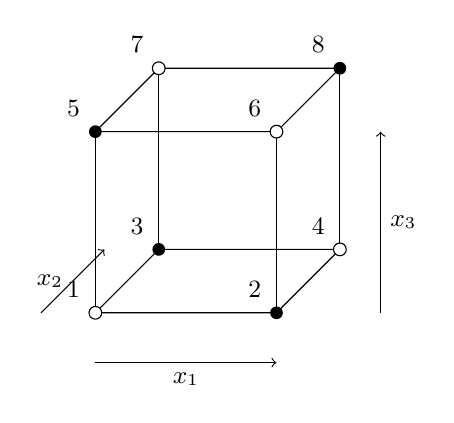
\begin{tikzpicture}[scale=1.15,every node/.style={font=\small}]
\coordinate (v1) at (0,0);\coordinate (v2) at (2,0);
\coordinate (v3) at (.7,.7);\coordinate (v4) at (2.7,.7);
\coordinate (v5) at (0,2);\coordinate (v6) at (2,2);
\coordinate (v7) at (.7,2.7);\coordinate (v8) at (2.7,2.7);
\draw (v1)--(v2)--(v4)--(v3)--cycle;
\draw (v5)--(v6)--(v8)--(v7)--cycle;
\draw (v1)--(v5) (v2)--(v6) (v3)--(v7) (v4)--(v8);
\foreach \i in {1,4,6,7}{\draw[fill=white] (v\i) circle (2pt);}
\foreach \i in {2,3,5,8}{\fill (v\i) circle (2pt);}
\foreach \i in {1,...,8}{\node[above left=2pt] at (v\i) {\i};}
\draw[->] (0,-.55)--node[below] {$x_1$}(2,-.55);
\draw[->] (3.15,0)--node[right] {$x_3$}(3.15,2);
\draw[->] (-.6,0)--node[left] {$x_2$}(.1,.7);
\end{tikzpicture}
\caption{The full three-factor cube in standard order. Filled vertices have
\(x_1x_2x_3=1\); open vertices have product \(-1\). The same partition
defines two half fractions or two blocks. This records the cube and
alternate-corner constructions of the selected NIST sections.}
\label{fig:p15-factorial-cube}
\end{figure}

\section{Run order, center points, and blocked factorials}
\label{sec:p15-factorial-execution}

The polishing example uses the following low, middle and high settings:
\[
\begin{array}{c|rrr}
 &-1&0&1\\\hline
\text{Speed}&16&20&24\\
\text{Feed}&0.001&0.003&0.005\\
\text{Depth setting}&0.010&0.015&0.020
\end{array}.
\]
Coding is \((u-u_0)/h\), with half-ranges \(4,0.002,0.005\),
respectively. The full replicated table is the eight standard-order rows
above followed by the same eight rows. The source's randomized order of
those sixteen labeled runs is
\[
 5,15,9,7,3,12,6,4,2,13,8,16,1,14,11,10.
\]
Its nineteen-run schedule inserts \((0,0,0)\) at positions 1, 9 and 19
and fills the other positions in that order. These specifications recover
every row of its Tables 3.5--3.9. Running the original standard order could
align the third factor's four-low/four-high pattern with day/night drift;
randomization and recording execution conditions address that risk.

\begin{hbtheorem}{thm:p15-factorial-centers-blocks}{proved=annex:p15.factorial.centers-blocks}{What centers and block columns identify}
For a three-factor full factorial split by \(b(x)=x_1x_2x_3\), block I
contains rows \(1,4,6,7\) and block II rows \(2,3,5,8\).
On these eight corner rows the block column equals the three-factor
interaction column. A model with
both a free block coefficient \(\gamma\) and \(\beta_{123}\) identifies
their sum, while the main and two-factor columns remain orthogonal to it.
If the center is then observed in both blocks, a common center response
with additive block effects gives a between-block center contrast
\(2\gamma\). Combining it with the corner contrast
\(2(\gamma+\beta_{123})\) separates \(\gamma\) and \(\beta_{123}\)
under that enlarged model.

In a quadratic response model
\(\beta_0+\sum_j\beta_jx_j+\sum_{i<j}\beta_{ij}x_ix_j
 +\sum_jq_jx_j^2\), the mean at the center minus the equally weighted
corner mean is \(-\sum_jq_j\). Corners and the common center do not
separate the individual \(q_j\), because their square columns coincide.
Adding center rows to the fraction \(x_3=x_1x_2\) likewise does not
separate \(\beta_3\) from \(\beta_{12}\).
\end{hbtheorem}

The corner-only block construction gives up a high-order comparison.
Interpreting its fitted block coefficient as a pure block effect requires
an assumption about the aliased interaction. Center points provide repeated
observations and a curvature or drift diagnostic under the corresponding
model; they do not identify every quadratic term or remove every alias.
Within-block replication and randomization retain their own assignment unit.

\section{Regular fractions, generators, and aliases}
\label{sec:p15-factorial-fractions}

\begin{hbdefinition}{def:p15-factorial-fraction}{A regular two-level fraction}
Represent a word by a subset \(S\subseteq\{1,\ldots,k\}\), with
column \(\chi_S\). Multiplication is symmetric difference:
\(\chi_S\chi_T=\chi_{S\mathbin{\triangle}T}\), and the empty word
is the intercept \(I\). A regular fraction is specified by \(p\)
independent word equations
\(\chi_{G_j}=s_j\), with \(s_j\in\{-1,1\}\).
Independence means that no nonempty product of the selected generator words
is the empty word.
Their products form a group \(\mathcal G\) of \(2^p\) words, with
assigned signs \(s(H)\). The full defining relation includes every
nonempty word in this group, not only the chosen generators. Positive
generator signs give the principal fraction.
\end{hbdefinition}

\begin{hbtheorem}{thm:p15-factorial-alias}{proved=annex:p15.factorial.alias}{Run count and the exact alias relation}
The regular fraction has \(2^{k-p}\) runs and
\[
 \frac1{2^{k-p}}\sum_{x\text{ in fraction}}\chi_S(x)\chi_T(x)
 =\begin{cases}s(S\mathbin{\triangle}T),&S\mathbin{\triangle}T\in\mathcal G,\\
 0,&\text{otherwise}.
 \end{cases}
\]
Columns in the same word coset are identical up to their stated signs;
columns from different cosets are orthogonal. For a full factorial mean
function \(\sum_T\beta_T\chi_T\), the normalized contrast on a fraction
has expectation
\[
 \mathbb E\!\left[\frac1{2^{k-p}}\sum_x\chi_S(x)Y_x\right]
   =\sum_{H\in\mathcal G}s(H)\beta_{S\mathbin{\triangle}H}.
\]
It estimates this alias sum without an assumption that the other terms vanish.
\end{hbtheorem}

\begin{hbdefinition}{def:p15-factorial-resolution}{Resolution and aberration}
The resolution is the smallest size of a nonempty word in the defining
relation. Its usual label is a Roman numeral. The word-length counts record
how many defining words have each size; comparisons of aberration examine
these counts from the shortest lengths upward. Such a comparison is about
an alias pattern, not evidence that the aliased physical effects are small.
A full factorial, whose defining group has no nonempty word, may be assigned
infinite resolution for these comparisons.
\end{hbdefinition}

\begin{hbcorollary}{thm:p15-factorial-resolution}{proved=annex:p15.factorial.resolution}{Resolution III, IV, and V}
At resolution III, distinct main effects are not aliased, but some main
effects are aliased with two-factor interactions. At resolution IV, main
effects are clear of all two-factor interactions, while some two-factor
interactions are mutually aliased. At resolution V, main effects and
two-factor interactions are clear of one another, but some two-factor
interactions are aliased with three-factor interactions. These statements
do not separate any effect from every possible higher-order interaction.
For resolution at least V, the intercept, all \(k\) main effects and all
\(\binom{k}{2}\) two-factor columns are linearly independent. Thus
\(N\geq1+k+\binom{k}{2}\). For eight factors this is \(N\geq37\);
a regular power-of-two fraction therefore needs at least sixty-four runs.
\end{hbcorollary}

A resolution-II design aliases some main effects with one another. It may
still estimate a specified sum or other row-space functional; it does not
supply their separate values without additional information.

\section{The half fraction and the cost of a sparsity assumption}
\label{sec:p15-factorial-half}

The following table gives the two-factor base, its product column, and both
three-factor half fractions. It retains the constructions of the source's
Tables 3.12--3.15:
\[
\begin{array}{c|rr|r|rr}
 &x_1&x_2&x_1x_2&x_3=+x_1x_2&x_3=-x_1x_2\\\hline
1&-1&-1&1&1&-1\\2&1&-1&-1&-1&1\\
3&-1&1&-1&-1&1\\4&1&1&1&1&-1
\end{array}.
\]
For the principal fraction, \(I=123\), and the complete alias classes are
\[
 I=123,\qquad 1=23,\qquad2=13,\qquad3=12.
\]
The last two analysis columns \(x_3,x_1x_2\) coincide. Replacing
\((\beta_3,\beta_{12})\) by
\((\beta_3+t,\beta_{12}-t)\) leaves every fitted response unchanged.
Only their sum is recovered. For the negative fraction the signs reverse:
\(I=-123\), \(1=-23\), \(2=-13\), \(3=-12\).

\begin{hbexample}{def:p15-factorial-nist-effects}{Full and fractional contrasts in the source data}
The source's standard-order responses are
\[
 (33,63,41,57,57,51,59,53).
\]
Its full factorial has intercept \(51.75\) and factorial effects in order
\((1,2,12,3,13,23,123)\) equal to
\[
 (8.5,1.5,-3.5,6.5,-14.5,0.5,3.5).
\]
On rows \(1,4,6,7\), the negative fraction, the three main-column
contrasts are \((8,16,10)\). They equal
\((8.5-0.5,\,1.5-(-14.5),\,6.5-(-3.5))\), precisely the predicted
alias differences. The corresponding principal-fraction contrasts are
\((9,-13,3)\). There is no conflict between these computations: the
fractions estimate different sums of full factorial effects.
\end{hbexample}

In the source's fifteen-run budget example, a twice-replicated full cube
already requires sixteen runs. A twice-replicated half fraction uses eight,
leaving seven for centers and contingencies. Its displayed thirteen-run
schedule is
\[
 000,\ +--,\ -+-,\ 000,\ +++,\ --+,\ 000,\ +--,
 \ --+,\ 000,\ +++,\ -+-,\ 000.
\]
Here the third coordinate is the product of the first two at the corners;
the center indicator is one exactly on the five \(000\) rows. This
specifies every row of Table 3.16. If interactions matter, an unreplicated
full cube plus centers may instead preserve the necessary effect separation.
Neither choice removes the need to justify its variance and mean model.

\section{Eight-factor designs and the source catalogue}
\label{sec:p15-factorial-eight}

For eight factors in thirty-two runs, the first source construction starts
with five freely varied columns and generates
\[
 6=345,\qquad7=1245,\qquad8=1235.
\]
Its full defining relation is
\[
 I=3456=12457=12358=12367=12468=3478=5678.
\]
Together with the standard-order formula in
\cref{def:p15-factorial-walsh}, these equations specify the complete
thirty-two-row design matrix. The resolution is IV. The aliased two-factor
groups are
\[
 34=56=78,\quad35=46,\quad36=45,\quad37=48,
 \quad38=47,\quad57=68,\quad58=67.
\]
These involve fifteen of the twenty-eight two-factor interactions.
The thirteen involving factor 1 or factor 2 are clear of other two-factor
interactions, though higher-order aliases remain.

The source's alternative \(6=12345,7=135,8=245\) has defining relation
\[
 I=123456=1357=2458=2467=1368=123478=5678.
\]
Its two-factor alias groups are
\[
\begin{gathered}
13=57=68,\quad15=37,\quad17=35,\quad24=58=67,\\
25=48,\quad28=45,\quad26=47,\quad27=46,\\
16=38,\quad18=36,\quad56=78.
\end{gathered}
\]
Exactly four two-factor interactions, \(12,14,23,34\), are clear of other
two-factor interactions. Thus twenty-four are aliased. The five length-four
words make this pattern less favorable than the first construction's three
length-four words under the stated short-word comparison.

A third displayed specification is \(6=123,7=124,8=2345\). It is a
relabeling of the first defining group by
\[
 (1,2,3,4,5,6,7,8)\longmapsto(5,8,1,2,3,6,4,7).
\]
The image of its three original generators spans the same word group,
so the alias structure is unchanged up to this factor permutation.

The following catalogue preserves all design specifications in the selected
2012 Table 3.17. An entry \((k,p;R;N)\) denotes \(2^{k-p}_R\), with
\(k\) factors, \(p\) independent generators, resolution label \(R\)
and \(N\) runs. It is a source catalogue, not a claim that a design's
resolution alone meets a particular scientific target.
\[
\begin{array}{rrrr|rrrr|rrrr}
k&p&R&N&k&p&R&N&k&p&R&N\\\hline
3&1&\mathrm{III}&4&4&1&\mathrm{IV}&8&5&1&\mathrm V&16\\
5&2&\mathrm{III}&8&6&1&\mathrm{VI}&32&6&2&\mathrm{IV}&16\\
6&3&\mathrm{III}&8&7&1&\mathrm{VII}&64&7&2&\mathrm{IV}&32\\
7&3&\mathrm{IV}&16&7&4&\mathrm{III}&8&8&1&\mathrm{VIII}&128\\
8&2&\mathrm V&64&8&3&\mathrm{IV}&32&8&4&\mathrm{IV}&16\\
9&2&\mathrm{VI}&128&9&3&\mathrm{IV}&64&9&4&\mathrm{IV}&32\\
9&5&\mathrm{III}&16&10&3&\mathrm V&128&10&4&\mathrm{IV}&64\\
10&5&\mathrm{IV}&32&10&6&\mathrm{III}&16&11&4&\mathrm V&128\\
11&5&\mathrm{IV}&64&11&6&\mathrm{IV}&32&11&7&\mathrm{III}&16\\
15&11&\mathrm{III}&16&31&26&\mathrm{III}&32&&&&
\end{array}
\]
The source also identifies a sixty-four-run resolution-V option for eight
factors and a forty-eight-run three-quarter alternative. The latter is
not a regular power-of-two fraction governed by the word-group formula.
Its separate construction and the linked Dataplot catalogue files are
external source referrals, not additional rows in the selected compiled
sections. For letter notation, factors 1 through 11 correspond to
\(A,B,C,D,E,F,G,H,J,K,L\); \(I\) denotes the intercept.
The sixteen-run, fifteen-factor and thirty-two-run, thirty-one-factor
entries are saturated for a main-effects model: even that restricted model
uses every observation-space dimension.

Screening designs trade run count against reliance on small-interaction
assumptions. Follow-up designs may add runs to separate important aliases
or add levels to study curvature. Different generators with the same run
count and resolution can protect different contrasts. A contrast should
therefore be checked against the actual defining relation or the row space,
not inferred from a resolution label alone.

\section{Assignment effects and mechanism claims}
\label{sec:p15-factorial-causal}

\begin{hbdefinition}{def:p15-factorial-assignment}{A finite assignment experiment}
Fix \(N\geq1\) recruited units, a nonempty finite set of treatment cells
\(\mathcal T\), and real potential responses \(Y_i(t)\).
Let \(Z_i\) be the randomized assigned
cell and \(\pi_i(t)=\Pr(Z_i=t)>0\). Stable treatment versions,
consistency and no relevant interference mean that the recorded outcome
for a retained unit is \(Y_i(Z_i)\). Randomness here is the known
assignment mechanism; it is separate from random sampling of a population.
For fixed weights \(w_t\), define
\(\tau=N^{-1}\sum_i\sum_tw_tY_i(t)\).
\end{hbdefinition}

\begin{hbtheorem}{thm:p15-factorial-assignment}{proved=annex:p15.factorial.assignment}{Which assignment contrast is unbiased?}
Under the preceding assignment model,
\[
 \widehat\tau=\frac1N\sum_i\sum_t
  \frac{w_t\mathbf1_{\{Z_i=t\}}Y_i(t)}{\pi_i(t)}
\]
is unbiased for \(\tau\). For a completely randomized design with fixed
positive cell sizes \(n_t\), it equals \(\sum_tw_t\overline Y_t\).
Its exact randomization variance is
\[
 \frac1{N^2}\sum_{i,t,j,u}
 \frac{w_tw_uY_i(t)Y_j(u)}{\pi_i(t)\pi_j(u)}
 \bigl(\pi_{ij}(t,u)-\pi_i(t)\pi_j(u)\bigr),
\]
where \(\pi_{ij}(t,u)=\Pr(Z_i=t,Z_j=u)\), also for \(i=j\).
This identity can involve unobserved potential responses; it is not itself
an observable variance estimator.
\end{hbtheorem}

For the P19 targets, use weights \((0,0,-1,1)\) for the aid-present
checking contrast and \((-1,1,-1,1)/2\) for its equal-weight average.
Blocked assignment uses its actual marginal and joint probabilities and
the desired block weights. Differential missing outcomes, incompatible
unit definitions or interference can break the displayed observation
model. Noncompliance does not change an assignment contrast into an effect
of receiving the instruction. Generalization beyond the recruited units
requires a sampling or transport argument.

\begin{hbtheorem}{thm:p15-factorial-mechanism}{proved=annex:p15.factorial.mechanism}{The factorial surface does not identify a psychological mechanism}
There exist two finite causal models with the same responses under every
assignment of checking \(A\) and aid \(B\), including the surface
\(4-4A-4B+6AB\), but different responses to intervening on a putative
reflection variable. Hence complete estimation of the factorial surface,
even without sampling error, does not identify that mechanism.
\end{hbtheorem}

The required additional evidence concerns the competing mechanisms:
process measurements with an explicit measurement model, interventions or
controls that separate them, and assumptions connecting those observations
to the causal equations. Statistical estimability, model-based uncertainty,
an effect of randomized assignment and a mechanism interpretation each have
their own premises. The distinction agrees with the intervention and
identification definitions in \cref{def:p16-causal-intervention,def:p16-causal-identification}.

% ED26-METHOD-imprecise-probability mathematical component draft.
% Exact Walley2014 article acquisition remains open in the source note.
\chapter{Imprecise Probability and Lower-Prevision Reasoning}
\label{sec:p15-imprecise-probability}

A lower probability records a bound on an event; a lower prevision records
a bound on the value of a gamble. Coherence constrains their joint use.
It neither selects a uniquely true distribution nor requires every pair of
decisions to be ranked. The bounded-gamble construction here follows the
identified author manuscript of Miranda
\cite[author manuscript, §§2--4]{MirandaCoherentLowerPrevisionsCapture}.
The separation and finitely additive integration premises are proved in
\cref{thm:p17-mmeu-hahn-banach,thm:p17-mmeu-charges-compactness}.
The ambient set theory includes Choice as in that treatment.

\section{Gambles, prices and domains}
\label{sec:p15-ip-domains}

\begin{hbdefinition}{def:p15-ip-domain}{The bounded-gamble domain}
Let \(\Omega\ne\varnothing\). A gamble is a bounded real function on
\(\Omega\), with rewards expressed in a specified linear utility scale.
Write \(\mathcal L(\Omega)\) for all such functions.
More generally let \(\Sigma\) be an algebra of subsets of \(\Omega\),
and let \(B(\Sigma)\) be the uniform closure of its finite-valued simple
functions. Put \(B=B(\Sigma)\). It contains constants and event indicators
\(I_A\), \(A\in\Sigma\), and is closed under products.
For \(\Sigma=\mathcal P(\Omega)\) it is exactly \(\mathcal L(\Omega)\).
On a sigma algebra it is exactly the bounded measurable functions.
An assessment domain \(\mathcal K\subseteq B\) need not be linear,
finite or closed under negation.
\end{hbdefinition}

\begin{hbdefinition}{def:p15-ip-prices}{Lower and upper previsions}
A lower assessment \(\underline P:\mathcal K\to\mathbb R\) specifies
supremum acceptable buying prices. It licenses the transaction
\(f-\underline P(f)+\epsilon\) for each \(\epsilon>0\), without
specifying acceptance at the endpoint \(\underline P(f)\).
An upper assessment is an infimum selling price. The conjugate upper
prevision on \(-\mathcal K\) is
\[
 \overline P(-f)=-\underline P(f)\qquad(f\in\mathcal K).
\]
When all relevant indicators are in the domain, use
\(\underline P(A)=\underline P(I_A)\) and
\(\overline P(A)=\overline P(I_A)\).
Imprecision of a utility-valued price and imprecision of an event
probability are distinct inputs. For monetary rewards a linear utility
scale is an additional modelling assumption.
\end{hbdefinition}

\begin{hbdefinition}{def:p15-ip-coherence}{Avoiding sure loss and coherence}
Put \(G(f)=f-\underline P(f)\). The assessment avoids sure loss when
\[
 \sup_{\omega\in\Omega}\sum_{i=1}^n s_iG(f_i)(\omega)\geq0
 \quad(n\geq0,\ f_i\in\mathcal K,\ s_i\geq0).
\]
It is coherent when it avoids sure loss and also, for every such finite
portfolio, \(f_0\in\mathcal K\) and \(s_0\geq0\),
\[
 \sup_{\omega\in\Omega}
 \left[\sum_{i=1}^n s_iG(f_i)-s_0G(f_0)\right](\omega)\geq0.
\]
Only one assessed gamble is sold, possibly at multiple stakes. This
condition prevents the other accepted buying transactions from forcing
an increase of its stated supremum buying price. A linear prevision
instead permits arbitrary finite buying and selling portfolios.
\end{hbdefinition}

\begin{hblemma}{thm:p15-ip-stakes}{proved=annex:p15.ip.stakes}{Integer and real stakes}
The preceding conditions are unchanged if stakes are initially restricted
to nonnegative integers with repeated occurrences of a gamble.
\end{hblemma}

\section{Natural extension and compatible precise models}
\label{sec:p15-ip-extension}

\begin{hbdefinition}{def:p15-ip-natural-extension}{Natural extension of an assessment}
For \(g\in B\), define
\[
 \underline E(g)=\sup\left\{\alpha\in\mathbb R:
 g-\alpha\geq\sum_{i=1}^n s_i
             [f_i-\underline P(f_i)],\quad
 n\geq0,\ f_i\in\mathcal K,\ s_i\geq0\right\}.
\]
The inequality is pointwise and the empty portfolio is allowed.
Equivalently take the supremum over portfolios of
\(\inf_\Omega[g-\sum_i s_iG(f_i)]\).
\end{hbdefinition}

\begin{hbtheorem}{thm:p15-ip-natural-extension}{proved=annex:p15.ip.natural-extension}{Existence, coherence and least commitment}
If \(\underline P\) avoids sure loss, \(\underline E\) is finite,
coherent on \(B\), and the least coherent lower prevision on \(B\)
dominating \(\underline P\) on \(\mathcal K\). It satisfies
\[
\begin{gathered}
 \inf g\leq\underline E(g)\leq\sup g,\qquad
 \underline E(c)=c,\qquad
 \underline E(g+c)=\underline E(g)+c,\\
 \underline E(tg)=t\underline E(g)\ (t\geq0),\qquad
 \underline E(g+h)\geq\underline E(g)+\underline E(h),\\
 g\leq h\Longrightarrow\underline E(g)\leq\underline E(h),\qquad
 |\underline E(g)-\underline E(h)|\leq\|g-h\|_\infty.
\end{gathered}
\]
It agrees with the input on \(\mathcal K\) exactly when the input is
coherent. If the input incurs sure loss, \(\underline E(g)=+\infty\)
for every \(g\); it then supplies no finite coherent extension.
\end{hbtheorem}

\begin{hbtheorem}{thm:p15-ip-linear-domain}{proved=annex:p15.ip.linear-domain}{Coherence on the full vector domain}
A real functional \(I:B\to\mathbb R\) is a coherent lower prevision
if and only if
\[
 I(g)\geq\inf g,\qquad I(tg)=tI(g)\ (t>0),\qquad
 I(g+h)\geq I(g)+I(h).
\]
These conditions imply the displayed bounds, cash translation, monotonicity
and Lipschitz properties in \cref{thm:p15-ip-natural-extension}.
Oddness and additivity are additional
conditions; they do not follow from positive homogeneity.
\end{hbtheorem}

\begin{hbdefinition}{def:p15-ip-compatible}{Compatible linear previsions and probabilities}
A precise model is a positive normalized linear functional \(L\) on \(B\).
It corresponds to a finitely additive probability on \(\Sigma\), with
\(L(I_A)=L(A)\); its expectation is the uniform simple-function integral.
The compatible set is
\[
 \mathcal M(\underline P)=
 \{L:\ L\text{ is positive normalized linear on }B,
                   \ L(f)\geq\underline P(f)\ (f\in\mathcal K)\}.
\]
Use the eventwise, equivalently the bounded-integral, weak-star topology.
No countable additivity assumption has been inserted.
\end{hbdefinition}

\begin{hbtheorem}{thm:p15-ip-representation}{proved=annex:p15.ip.representation}{Representation on arbitrary assessment domains}
Avoidance of sure loss is equivalent to
\(\mathcal M(\underline P)\ne\varnothing\). In that case this set is
compact and convex, \(\mathcal M(\underline P)=\mathcal M(\underline E)\),
and
\[
 \underline E(g)=\min_{L\in\mathcal M(\underline P)}L(g)\qquad(g\in B).
\]
The input is coherent exactly when its values on \(\mathcal K\) equal
these minima. For a coherent functional on all of \(B\), its compatible
set is the unique nonempty closed convex representing set. This uniqueness
does not apply to an arbitrary proposed prior subset when only a restricted
assessment domain has been elicited.
\end{hbtheorem}

\begin{hbcorollary}{thm:p15-ip-dual}{proved=annex:p15.ip.dual}{Upper envelopes and event conjugacy}
Set \(\overline E(g)=-\underline E(-g)\). Then
\[
 \overline E(g)=\max_{L\in\mathcal M(\underline P)}L(g),\qquad
 \underline E(g)\leq\overline E(g),\qquad
 \overline E(A)=1-\underline E(A^c).
\]
Natural extension through an intermediate domain has the same final
answer as direct extension, provided that intermediate assessments are
the natural-extension values.
\end{hbcorollary}

For the remainder of the chapter assume that the input avoids sure loss,
so that \(\underline E\) and its nonempty compatible set are defined
with the preceding properties.

\section{Finite additivity and countable additivity}
\label{sec:p15-ip-additivity}

\begin{hbtheorem}{thm:p15-ip-countable-additivity}{proved=annex:p15.ip.countable-additivity}{The extra continuity condition}
Suppose \(\Sigma\) is a sigma algebra. Every member of
\(\mathcal M(\underline P)\) is countably additive if and only if,
for every sequence \(A_n\downarrow\varnothing\),
\[
                         \overline E(A_n)\longrightarrow0.
\]
Coherence alone does not imply this condition. On a countably infinite
space a free-ultrafilter probability is coherent but not countably
additive. Even \(\underline E(A_n)\to0\) for every such sequence does
not suffice: the vacuous lower prevision \(\underline E(g)=\inf g\)
has that lower continuity and admits non-countably-additive precise models.
\end{hbtheorem}

Requiring countably additive compatible models is therefore a substantive
extra assumption. It can change compactness, attainment and the available
models. The indicator of a conditioning event must belong to the selected
event algebra; an undefined probability of a set outside that algebra is
not a zero probability.

\section{Event bounds do not determine all gamble bounds}
\label{sec:p15-ip-event-information}

\begin{hbtheorem}{thm:p15-ip-event-separation}{proved=annex:p15.ip.event-separation}{Equal event envelopes, different coherent gamble prices}
On \(\Omega=\{1,2,3\}\), let \(C\) be the convex hull of all six
permutations of \((1,3,6)/10\), and let \(D\) be the hull with
\((1,3,6)/10\) omitted. Their lower probabilities agree on every event:
zero on the empty event, \(1/10\) on singletons, \(2/5\) on pairs,
and one on the whole space. Their upper probabilities also agree.
But for \(f=(2,1,0)\),
\[
                \min_C E_p f=1/2,\qquad \min_D E_p f=7/10.
\]
The decision against the certain payoff \(3/5\) consequently changes
under a stated maxmin rule. The missing gamble information cannot be
recovered by simply assigning a precise number within each event interval.
\end{hbtheorem}

Belief/plausibility and possibility/necessity are separately defined event
constructions in \cref{def:p14-evidence-uncertainty-data}. Under its finite
mass-allocation assumptions, \cref{thm:p14-evidence-finite-measures}
supplies the belief/plausibility allocated probability envelopes. Taking expected
values under those probabilities also supplies coherent lower previsions
by \cref{thm:p15-ip-representation}; the special model's assumptions
determine which probabilities are retained. The explicit coherent lower
probability which fails the belief-function inequality in
\cref{thm:p14-evidence-measure-separation} proves that general coherent
lower probabilities need not be belief functions. A possibility union law
uses a maximum, rather than the additive law of a probability.
These representations cannot be identified solely by the common range
\([0,1]\), and their conditioning or evidence-combination rules require
their own hypotheses.
\Cref{sec:p15-w02b-p15-034-evidence-models} proves that the gamble
extension of a belief function is the focal-set minimum sum, equal to its
Choquet value (\cref{thm:p15-w02b-p15-034-belief-extension}); that a
coherent lower prevision can agree with a belief function on every event
and still differ from that extension
(\cref{thm:p15-w02b-p15-034-belief-not-prevision}); that necessity
measures form a proper subclass of belief functions
(\cref{thm:p15-w02b-p15-034-strict-classes}); and that Dempster
conditioning of a belief function or a possibility measure need not be
jointly coherent with the natural extension
(\cref{thm:p15-w02b-p15-034-dempster}).

\begin{hblemma}{thm:p15-ip-possibility-bridge}{proved=annex:p15.ip.possibility-bridge}{A normalized finite possibility model as a coherent envelope}
For the finite normalized possibility distribution in
\cref{def:p14-evidence-uncertainty-data}, order the outcomes so that
\(1=\pi_1\geq\cdots\geq\pi_n\geq0\), and put
\(\pi_{n+1}=0\). The nested focal sets
\(B_i=\{\omega_1,\ldots,\omega_i\}\), with masses
\(m(B_i)=\pi_i-\pi_{i+1}\), have
\[
 \operatorname{Bel}_m(A)=\operatorname{Nec}_\pi(A),\qquad
 \operatorname{Pl}_m(A)=\operatorname{Poss}_\pi(A).
\]
Their allocated probabilities therefore give coherent lower/upper gamble
previsions extending these particular event bounds. The nested-focal-set
constraint is an additional restriction on the general model.
\end{hblemma}

\section{Conditional models for one observation event}
\label{sec:p15-ip-conditioning}

\begin{hbdefinition}{def:p15-ip-conditional}{Conditional prices and compatible pairs}
Let \(A\in\Sigma\), \(A\ne\varnothing\). A precise conditional
model \(Q\) is a positive normalized linear functional on \(B\),
supported on \(A\): \(Q(I_A)=1\). A pair \((L,Q)\) is Bayes-compatible
when
\[
                   L(I_Ag)=L(A)Q(g)\qquad(g\in B).
\]
For \(L(A)>0\) this determines \(Q\); for \(L(A)=0\) it constrains
none of its supported values. A conditional transaction has payoff
\(I_A[g-q]\), so it is called off outside \(A\).
Coherence of transactions made only on \(A\) is assessed on \(A\),
rather than being made automatic by the zero payoff outside it.
Joint coherence here tests every finite portfolio of unconditional and
conditional buying gains with at most one assessed gain sold, using
nonnegative stakes. The supremum is taken on the union of their active
conditioning events: on \(\Omega\) if an unconditional transaction is
present, and otherwise on \(A\). The separate conditional tests on
\(A\) are required as well.
These definitions concern one event. They do not assert a simultaneous
updating theorem for arbitrary infinite partitions.
\end{hbdefinition}

\begin{hbdefinition}{def:p15-ip-updates}{Natural and regular conditioning}
The natural conditional lower prevision is the infimum of \(Q(g)\)
over all Bayes-compatible pairs with \(L\in\mathcal M(\underline P)\).
For \(\overline E(A)>0\), the regular extension is
\[
 \underline R(g\mid A)=
 \inf_{\substack{L\in\mathcal M(\underline P)\\L(A)>0}}
                         \frac{L(I_Ag)}{L(A)}.
\]
If \(\overline E(A)=0\), define it to be \(\inf_A g\); this case
contains no positive-probability Bayesian conditional. Upper conditional
previsions are the conjugates on \(A\).
\end{hbdefinition}

Interpreting a contingent price as a future price after learning \(A\)
requires an updating principle relating transactions accepted after that
information to their called-off transactions before it, with no additional
information from the observation mechanism. This is a modelling premise,
rather than a consequence of the numerical bounds alone
\cite[author manuscript, §3.1]{MirandaCoherentLowerPrevisionsCapture}.
At lower probability zero, coherence permits several conditional models.
Choosing regular extension adds a commitment by excluding the zero-\(A\)
precise models from that conditional calculation; the displayed formulas
do not claim that coherence alone uniquely chooses this updating rule.

\begin{hbtheorem}{thm:p15-ip-conditional-models}{proved=annex:p15.ip.conditional-models}{The three probability boundaries}
Natural and regular conditional lower previsions are coherent on the
gamble space restricted to \(A\). If \(\underline E(A)>0\), they agree,
their Bayesian infimum is attained, and their value is determined by the
original assessment. If \(\underline E(A)=0<\overline E(A)\), natural
conditioning is vacuous, \(\inf_A g\), while regular conditioning can
be more informative. If \(\overline E(A)=0\), both are vacuous under
the stated convention. On this single-event domain the conditional models
are jointly coherent with the original unconditional assessment. Regular
conditioning, when \(\overline E(A)>0\), preserves its unconditional
envelope by the density of
positive-\(A\) models in the original compatible set.
\end{hbtheorem}

\begin{hbtheorem}{thm:p15-ip-generalized-bayes}{proved=annex:p15.ip.generalized-bayes}{Generalized Bayes rule and its zero boundary}
For \(\underline E(A)>0\), the equation
\[
                       \underline E(I_A[g-q])=0
\]
has exactly one root, namely \(q=\underline R(g\mid A)\).
For \(\underline E(A)=0<\overline E(A)\), its roots are every
\(q\leq\underline R(g\mid A)\); choosing an unspecified root then
does not define an update. Its largest root is regular extension.
\end{hbtheorem}

\begin{hbtheorem}{thm:p15-ip-conditional-bounds}{proved=annex:p15.ip.conditional-bounds}{What joint coherence actually forces at one event}
Let a full-domain conditional lower prevision \(C(\cdot\mid A)\)
be separately coherent and jointly coherent with \(\underline E\)
under \cref{def:p15-ip-conditional}. Then for every \(g\in B\),
\[
              \underline E(I_A[g-C(g\mid A)])=0.
\]
If \(\underline E(A)>0\), it follows that \(C=\underline R\).
If \(\underline E(A)=0<\overline E(A)\), its pointwise bounds are
\[
                    \inf_A g\leq C(g\mid A)\leq\underline R(g\mid A).
\]
Both limiting functionals are jointly coherent, so natural conditioning
is the least and regular conditioning the greatest on this single-event
domain. This conclusion does not select which intermediate coherent
assessments the subject actually supplies.
\end{hbtheorem}

\begin{hbexample}{def:p15-ip-zero-example}{A nonvacuous regular update at lower probability zero}
On \(\{a,b,c\}\) retain all distributions satisfying \(p_c\geq p_a\).
For \(A=\{a,c\}\), lower and upper probability are zero and one.
Natural conditioning gives lower probability zero to \(\{c\}\),
while regular conditioning gives \(1/2\): every retained positive-\(A\)
distribution has \(p_c/(p_a+p_c)\geq1/2\), with equality possible.
The prior concentrated at \(b\) explains the natural vacuity.
This is a calculation under specified models, not permission to divide
by the lower probability of \(A\).
It is the source's finite Example 1
\cite[author preprint, p.~2]{DeBockDeCooman2015ConditioningPreprint}.
\end{hbexample}

\section{Decision comparisons and independence assumptions}
\label{sec:p15-ip-decision-independence}

To assess robust improvement of \(f\) over \(g\), calculate
\(\underline E(f-g)\), as in \cref{def:p17-robust-dominance}.
Comparing \(\underline E(f)\) and \(\underline E(g)\) is the separate
maxmin rule. Complete utility information, a feasible menu and a stated
choice criterion are still needed; coherence alone does not specify them.
The vector example in \cref{thm:p15-ip-event-separation} uses common
known utility values, so its changed comparison is due to the retained
gamble information rather than a changed utility scale.

\begin{hbdefinition}{def:p15-ip-independence}{Specified notions of independence}
Epistemic irrelevance of \(Y\) for \(X\) requires that the conditional
lower prevision of every \(X\)-gamble after learning \(Y=y\) equals
its original marginal lower prevision. Epistemic independence requires
irrelevance in both directions. These are statements about the specified
conditional model. A strong product instead takes the closed convex hull
of all products of compatible marginal precise models, as in
\cref{def:p17-mmeu-product,thm:p17-mmeu-product-priors}.
The factorization concerns the generating products and their extreme-point
characterization, not every convex mixture. Logical independence of the
coordinates additionally means that the full product outcome space is
possible.
\end{hbdefinition}

\begin{hbtheorem}{thm:p15-ip-independence-boundary}{proved=annex:p15.ip.independence-boundary}{A product model does not settle null-event conditional prices}
Let \(X,Y\in\{0,1\}\). Retain the convex hull of product distributions
with \(p_X(1)\in[2/5,3/5]\), \(p_Y(1)\in[0,1]\).
The marginal lower probability of \(X=1\) is \(2/5\).
For \(A=\{Y=1\}\), its lower probability is zero, natural conditioning
gives \(\underline E(X=1\mid A)=0\), and regular conditioning gives
\(\underline R(X=1\mid A)=2/5\). Therefore any assertion of
irrelevance at the zero-lower-probability history must state which
conditional model, or which additional conditional assessments, it uses.
\end{hbtheorem}

A decision comparison that needs an independence judgement, with no
conditioning event of lower probability zero, is worked in
\cref{sec:p15-w02b-p15-034-independence-decision}: with imprecise binary
marginals, the agreement bet is robustly preferred to a sure payment under
the strong product, but the two acts stay unranked under the least
informative epistemically independent model and under the marginals alone
(\cref{thm:p15-w02b-p15-034-independence-models,thm:p15-w02b-p15-034-independence-decision}).

For infinite partitions, unconditional coherence does not by itself
justify simultaneous conditional assessments on every cell.
\Cref{sec:p15-w02b-p15-034-partition-updates} declares the
partition-update semantics, proves that a coherent partition update exists
exactly when the unconditional model is conglomerable for the partition
(\cref{thm:p15-w02b-p15-034-existence}), works a finitely additive
prevision with no partition update
(\cref{thm:p15-w02b-p15-034-counterexample}), and shows that the same
cellwise assessments pass Williams' finite-support criterion
(\cref{thm:p15-w02b-p15-034-williams}). The single-event results above
preserve their stated domain.

\chapter{Probability Quantifiers: Uniform Finite-Model Semantics}
\label{sec:p15-probability-quantifiers}

This is the finite-model presentation of \(L_{\omega P}\) in
Keisler--Lotfallah's author-hosted manuscript, especially its model
conventions on p.~3 and opening probability-quantifier treatment on
pp.~5--7 \cite{KeislerLotfallah2009AuthorProbability}. It is a distinct
presentation, not a reconstruction of Keisler's complete 1985 chapter
on probability quantifiers or its conditional-expectation operators.
The following semantic and translation proofs are supplied editorially.

\begin{hbdefinition}{def:p15-pq-models}{Two measures with different sample spaces}
Fix a nonempty finite relational vocabulary \(\nu\), without function
symbols. For \(n\ge1\), \(M_n\) is the set of all \(\nu\)-structures
on \(A=\{0,\ldots,n-1\}\). Fix \(p_R\in(0,1)\) for each relation
symbol. The measure \(\mu_n\) on \(M_n\) makes every ground relation
instance an independent Bernoulli event with parameter \(p_R\).
All subsets of this finite sample space are measurable.
The unbiased case has every \(p_R=1/2\).

Inside one fixed structure, a tuple of length \(\ell\) instead has
the uniform counting measure
\(\lambda_A^\ell(B)=|B|/n^\ell\) on \(A^\ell\).
Coordinates are sampled with replacement: syntactically distinct
variables may receive equal values. This tuple measure, not \(\mu_n\),
interprets a probability quantifier. The number
\(\mu_n(\theta)\) for a sentence is the probability of the model event
\(\{\mathcal A:\mathcal A\models\theta\}\).
\end{hbdefinition}

\begin{hbdefinition}{def:p15-pq-language}{The actual finitary formation and satisfaction clauses}
\(L_{\omega P}\) retains first-order equality, relation atoms, classical
Boolean connectives and ordinary quantifiers. If
\(\varphi(\bar x,\bar y)\) has exactly these free variables, with
the lists disjoint and without syntactic repetitions, then
\((\exists^{\ge r}\bar y)\varphi(\bar x,\bar y)\) is a formula,
binding \(\bar y\), for every real \(0<r<1\).
The source excludes probability quantifiers at \(0\) and \(1\).
Renaming and substitution are capture-avoiding.
For \(\bar a\in A^{|\bar x|}\),
\[
 \mathcal A\models(\exists^{\ge r}\bar y)\varphi(\bar a,\bar y)
 \quad\Longleftrightarrow\quad
 \frac{|\{\bar b\in A^{|\bar y|}:
                 \mathcal A\models\varphi(\bar a,\bar b)\}|}
      {n^{|\bar y|}}\ge r.
\]
Ordinary \(\forall\bar y,\exists\bar y\) abbreviate iterated
single-variable quantifiers; the probability binder counts tuples jointly.
Infinitary conjunctions belong to the separately named \(L_{\infty P}\);
they are not part of the fixed-size finitary translation below.
\end{hbdefinition}

\begin{hbtheorem}{thm:p15-pq-validities}{proved=annex:p15.pq.validities}{Semantic monotonicity and its boundary cases}
For these nonempty finite models, probability binders are monotone
in their scope and antitone in the threshold. For \(r,s\in(0,1)\),
\[
 \forall\bar y\,\varphi\ \Longrightarrow\
 (\exists^{\ge r}\bar y)\varphi\ \Longrightarrow\
 \exists\bar y\,\varphi.
\]
If \(r+s>1\), then
\((\exists^{\ge r}\bar y)\varphi\) implies
\(\neg(\exists^{\ge s}\bar y)\neg\varphi\).
Neither exchanging nested probability quantifiers nor replacing
negation by the complementary non-strict threshold is generally valid.
\end{hbtheorem}

\begin{hbexample}{def:p15-pq-order}{Order and threshold equality matter}
On three elements \(a,b,c\), let a binary relation have rows
\(\{a,b\},\{a,c\},\varnothing\), respectively.
Two rows contain at least two of the three elements, but only one column
does. Therefore
\((\exists^{\ge2/3}x)(\exists^{\ge2/3}y)R(x,y)\) is true,
whereas reversing the binders is false. On four elements with a unary
relation of size two, both half-threshold statements for that relation
and its complement are true. They are not each other's negations.
\end{hbexample}

\begin{hbtheorem}{thm:p15-pq-translation}{proved=annex:p15.pq.translation}{An exact size-indexed first-order translation}
For every fixed \(n\ge1\), finitary formulas have a capture-avoiding
first-order translation \(\tau_n\) preserving satisfaction in every
\(n\)-element structure and every parameter assignment.
A probability binder with \(\ell\) variables and threshold \(r\)
becomes the assertion that at least
\(k=\lceil rn^\ell\rceil\) pairwise distinct tuples satisfy the
translated scope. The annex gives the actual witness formula and both
directions, including the empty-tuple case.
This is a size-indexed translation, not uniform elimination on all
finite sizes. It is effective for rational thresholds; arbitrary real
threshold symbols have no assumed effective encoding.
\end{hbtheorem}

\begin{hbtheorem}{thm:p15-pq-limit-failures}{proved=annex:p15.pq.limit-failures}{Critical thresholds destroy unrestricted asymptotic claims}
For unbiased \(\mu_n\), the unary sentence
\((\exists^{\ge1/2}x)R(x)\) has limiting model probability \(1/2\),
not zero or one. With an unrestricted binary relation the sentence
\[
 \eta=\exists x\bigl[
  (\exists^{\ge1/2}y)R(x,y)\land
  (\exists^{\ge1/2}y)\neg R(x,y)\bigr]
\]
has probability zero at odd sizes and tends to one at even sizes.
Thus unrestricted \(L_{\omega P}\) has neither a zero--one law nor
a convergence law for this model distribution. This is the source's
Proposition~3.1 counterexample, with an independent complete proof.
The source's printed linear-exponent rate is not adopted; the annex
supplies a valid square-root-exponent bound and checks that distinction.
\end{hbtheorem}

The noncritical fragments, critical-value construction and elimination
proofs are developed separately in
\cref{sec:p15-probability-elimination}. They do not follow merely from
these basic clauses or \(\tau_n\), and their common-class, parameter
and size-dependent hypotheses must be retained.
No sound-and-complete calculus for the full language is claimed here.

The measure interfaces in \cref{def:p15-measure,def:p15-pushforward-law}
apply to the two finite measures once their sample spaces are declared.
P9's likelihood terms measure propositional world-events
(\cref{def:p09-likelihood-logic}); PCTL measures path events in a
transition model, with scheduler conventions on MDPs
(\cref{def:p09-pctl}). Pfeifer's primitive conditional-event prices and
coherence (\cref{def:p15-rat44-events,def:p15-rat44-coherence}) are different
again. None of their completeness, complexity or Bayes claims supplies
the quantified language treated here. Conversely this finite-model account
does not settle the original chapter's measure-model, completeness,
conditional-expectation or open-problem allocations.

\chapter{Noncritical Probability Quantifiers and Almost-Everywhere Elimination}
\label{sec:p15-probability-elimination}

Keisler--Lotfallah's held author manuscript develops this construction on
pp.~8--28; p.~29 completes its references
\cite{KeislerLotfallah2009AuthorProbability}. The present account retains
its critical-value test, ordinary existential witnesses, parameter equality
patterns, and distinction between weak and strong almost-everywhere
reduction. The proofs below are independent reconstructions; the
concentration argument deliberately does not assume independence of
evaluations at overlapping tuples. This later finite-model paper does not
replace the still-unavailable 1985 chapter.

Use the two sample spaces and satisfaction clauses of
\cref{def:p15-pq-models,def:p15-pq-language}. For the zero--one statements
here the finite relational vocabulary has positive arities and no
constants or function symbols. This guard matters: a nullary relation
whose model probability is \(p\in(0,1)\) is already a quantifier-free
sentence of probability \(p\). The unqualified extension to nullary
symbols would therefore be false. Parameters \(p_R\) are initially fixed
strictly between zero and one.

\begin{hbdefinition}{def:p15-pe-types}{Equality diagrams, complete types, and conditional limits}
For a list \(\bar x=(x_1,\ldots,x_k)\) of distinct variable symbols, an
equivalence relation \(E\) on its positions determines the equality
diagram \(D_E(\bar x)\): coordinates in the same class are equal and
coordinates in different classes are unequal. Write \(D(\bar x)\) for
the all-distinct diagram. A complete quantifier-free type \(\beta(\bar x)\)
specifies every relation atom on these variables and every equality,
consistently; it induces one such \(E\). The tuple \(\bar x_E\) replaces
each class by one variable, repeated at every position in that class.
Types and diagrams concern values, not merely variable spellings.

Extend the notation \(\mu_n(\theta(\bar x))\) by sampling both the random
structure and an independent uniform parameter tuple. For a
quantifier-free \(\alpha(\bar x,\bar y)\), with disjoint variable lists,
define
\[
 q_\beta(\alpha;\bar y)
   =\lim_{n\to\infty}
       \frac{\mu_n(\alpha(\bar x,\bar y)\land\beta(\bar x))}
            {\mu_n(\beta(\bar x))}.
\]
The denominator is positive once \(n\) realizes the equality classes.
The \(\bar y\)-critical values are the finitely many \(q_\beta\), over
all complete parameter types. The next result constructs the limit;
its definition does not assume that construction.
\end{hbdefinition}

\begin{hbtheorem}{thm:p15-pe-critical}{proved=annex:p15.pe.critical}{The actual critical-value computation}
Collapse the parameter equalities, evaluate parameter-only atoms by
\(\beta\), and evaluate equalities on otherwise distinct fresh coordinates.
Express the resulting Boolean formula in complete, mutually exclusive
truth patterns of its distinct remaining relation atoms. Then
\[
 q_\beta=\sum_{\text{satisfying patterns }v}
             \prod_{\text{distinct atom keys }t}
                  p_{R_t}^{v_t}(1-p_{R_t})^{1-v_t}.
\]
Identical atom keys are counted once. The empty Boolean cases give zero
or one. This finite sum proves existence of the conditional limit and
is a polynomial with integer coefficients in the atomic probabilities.
Each collapsed consistent type has a positive limiting probability.
For rational atomic probabilities the critical values are rational.
\end{hbtheorem}

\begin{hbdefinition}{def:p15-pe-content}{Noncritical syntax and quantifier-free content}
Noncriticality and \(\varphi^0\) are defined together, as in source
Definition~3.6. Quantifier-free formulas are noncritical and retain
themselves. Negation and conjunction are noncritical exactly when their
constituents are, and content commutes with these connectives. For an
ordinary single-variable binder, if \(\psi\) is noncritical, put
\[
 (\exists y\,\psi(\bar x,y))^0
   =\bigvee_{q_\beta(\psi^0;y)>0}\beta(\bar x)
       \ \vee\ \bigvee_{i=1}^{k}\psi^0(\bar x,x_i).
\]
For a probability binder its scope must be noncritical and its threshold
\(r\) must differ from every \(\bar y\)-critical value of \(\psi^0\);
then put
\[
 ((\exists^{\ge r}\bar y)\psi(\bar x,\bar y))^0
       =\bigvee_{q_\beta(\psi^0;\bar y)>r}\beta(\bar x).
\]
Empty disjunctions are false. Substitution is capture-avoiding.
For finitely many free variables, even an infinitary quantifier-free
Boolean combination can be replaced by a finite truth table on the
finitely many atoms. These clauses do not admit a critical tie by
changing \(>\) to \(\ge\).
\end{hbdefinition}

\begin{hbtheorem}{thm:p15-pe-uniform}{proved=annex:p15.pe.uniform}{Uniform elimination of one quantifier-free probability binder}
Let \(\alpha(\bar x,\bar y)\) be quantifier-free and let \(r\in(0,1)\)
be noncritical. With probability tending to one, the random structure
satisfies, simultaneously for every \(\bar a\in n^k\),
\[
 (\exists^{\ge r}\bar y)\alpha(\bar a,\bar y)
 \quad\longleftrightarrow\quad
       \bigvee_{q_\beta(\alpha;\bar y)>r}\beta(\bar a).
\]
All parameter equality patterns and all tuple collisions are included.
For a fixed formula the exceptional probability is at most a constant
times \(n^k e^{-c n}\), for some \(c>0\) and all sufficiently large \(n\).
The annex proves a finite-product bounded-difference estimate, including
its exponential-moment argument, rather than treating the tuple truth
indicators as independent.
\end{hbtheorem}

\begin{hbtheorem}{thm:p15-pe-elimination}{proved=annex:p15.pe.elimination}{Finitary noncritical elimination and its effective scope}
Every finitary noncritical \(\varphi(\bar x)\) satisfies
\[
 \lim_{n\to\infty}\mu_n
       \bigl(\forall\bar x(\varphi(\bar x)\leftrightarrow
                                      \varphi^0(\bar x))\bigr)=1.
\]
The ordinary existential clause is proved by actual fresh witnesses
and the explicit parameter-witness disjunction above. Structural
induction handles nested probability binders without exchanging them.
For sentences the content is true or false, giving a zero--one law.
For a fixed rational atomic-probability vector and rational threshold
syntax, noncriticality and content have finite recursive computations
(indeed primitive-recursive ones under usual finite syntax encodings).
No effectiveness for arbitrary real inputs is asserted.
\end{hbtheorem}

For example, for a binary relation with probability \(p\), the fresh
limit of \(R(x,y)\) is \(p\). A threshold below \(p\) has content true;
one above \(p\) has content false; equality is excluded. For the unary
scope \(y=x\), the fresh limit is zero, yet \(\exists y(y=x)\) has
content true through its parameter witness. This is why the second
disjunction in the ordinary existential clause cannot be dropped.

\begin{hbdefinition}{def:p15-pe-ae}{Weak and common-class reduction}
Two formulas are almost-everywhere equivalent when the model probability
of their universally closed equivalence tends to one. Weak reduction
allows a different asymptotic class for each formula. Strong reduction
requires one class \(C\) of finite structures, with
\(\mu_n(C\cap M_n)\to1\), on which every formula in the declared fragment
equals its chosen first-order content at every assignment.
Neither is a logical equivalence over all finite structures.
\end{hbdefinition}

\begin{hbtheorem}{thm:p15-pe-strong}{proved=annex:p15.pe.strong}{A common class for finitely many variables and thresholds}
Fix a variable budget \(k\) and a finite \(P_0\subset(0,1)\).
The noncritical fragment using these variables and only thresholds in
\(P_0\) strongly reduces to the \(k\)-variable quantifier-free fragment.
This includes well-founded infinitary conjunctions and disjunctions,
not just finitary formulas. The union over finite budgets and finite
threshold sets has formula-by-formula reduction and a zero--one law
for sentences. The proof constructs a finite set of primitive
quantifier-elimination identities before choosing the common class;
it does not intersect arbitrarily many asymptotic measure-one events.
\end{hbtheorem}

There is no common class for all thresholds, even with one variable:
for an unbiased unary \(R\), put \(r_m=1/2-1/m\), \(m\ge3\).
Every \((\exists^{\ge r_m}x)R(x)\) has true content, but their
conjunction is exactly the critical half-threshold assertion, of limiting
probability \(1/2\) by \cref{thm:p15-pq-limit-failures}.
Consequently an asymptotic measure-one class cannot realize all these
contents. This also supplies a noncritical infinitary counterexample
when infinitely many thresholds are allowed. The held manuscript's
p.~25 instead prints these below-half formulas as having asymptotic
measure zero and uses a disjunction; those two statements are not
adopted. The conjunction above is the independently checked correction.

\begin{hbdefinition}{def:p15-pe-parametric}{Parametric constraints and their actual conditioned model law}
A parametric sentence \(\pi\) is a finite conjunction of
\(\forall\bar z[D(\bar z)\to\tau(\bar z)]\), where \(\tau\) is a
Boolean combination of literals and every variable of \(\bar z\)
occurs in every literal. Assume \(\pi\) has models of every positive
finite size. The model measure is
\[
  (\mu_n\mid\pi)(B)=
            \frac{\mu_n(B\cap\{\mathcal A:\mathcal A\models\pi\})}
                 {\mu_n(\pi)}.
\]
Use only complete parameter types consistent with \(\pi\); their
conditional scope limits define \(q_\beta^\pi\), and the preceding
content clauses with those limits define \(\varphi^\pi\).
Conditioning does not preserve independence of individual atoms.
\end{hbdefinition}

\begin{hbtheorem}{thm:p15-pe-parametric}{proved=annex:p15.pe.parametric}{Parametric elimination through independent support blocks}
For this law, every finitary \(\pi\)-noncritical formula is
almost-everywhere equivalent to \(\varphi^\pi\), and its sentences have
a zero--one law. The limits \(q_\beta^\pi\) exist and are positive-type
conditional finite sums. The proof groups atoms by the exact set of
elements in their arguments: distinct support blocks remain independent
after conditioning, whereas atoms within one block can be correlated.
It constructs their normalized laws, the limits, the witness argument,
and concentration. It is not an inference from an unproved transfer of
the unconditioned theorem. The same finite primitive-identity argument
also gives the fixed-variable, finite-threshold common-class version.
\end{hbtheorem}

\begin{hbtheorem}{thm:p15-pe-model-boundaries}{proved=annex:p15.pe.model-boundaries}{What conditioning and the source's graph examples actually permit}
For a binary relation whose ordered ground atoms have probability \(p\),
conditioning on symmetry and irreflexivity makes the probability of a
distinct undirected edge
\[
             \frac{p^2}{p^2+(1-p)^2},
\]
not generally \(p\). This is an actual parametric class.
In contrast, in the ordinary vocabulary of one uncolored binary graph
relation, the class of all finite bipartite graphs cannot be a parametric
class in Definition~5.1's sense. The source's p.~22 mention of bipartite
graphs is therefore not adopted under this uncolored interpretation;
an additional presentation would have to be specified and justified.
If equality literals are permitted, a model whose size equals the
largest relation arity need not guarantee models of every size:
in a unary vocabulary the parametric constraint
\(\forall x y[D(x,y)\to x=y]\) has only singleton models.
The all-size hypothesis in \cref{def:p15-pe-parametric} is therefore
retained explicitly rather than inferred from that arity-only criterion.
The nullary-symbol extension of the zero--one assertions is also false,
by the one-atom countermodel already identified above.
\end{hbtheorem}

\begin{hbdefinition}{def:p15-pe-sequences}{The source's size-dependent noncriticality}
Now allow \(p_R(n)\in(0,1)\) and a threshold sequence \(r(n)\in(0,1)\).
For each complete \(\beta\), write
\(q_{\beta,n}=\mu_n[\alpha(\bar x,\bar y)\mid\beta(\bar x)]\);
these sequences need not converge. A sequence \(r(n)\) is critical for
\(\alpha\) if some \(\beta\) satisfies both
\[
 \liminf(q_{\beta,n}-r(n))\le0,\qquad
 \liminf(r(n)-q_{\beta,n})\le0.
\]
Otherwise the probability content selects the types with
\(\liminf(q_{\beta,n}-r(n))>0\).
For an ordinary existential with noncritical scope, every \(\beta\)
must satisfy either \(\liminf q_{\beta,n}>0\), or the logical validity
\[
 \forall\bar x\bigl(\beta(\bar x)\to
                       \bigvee_{i=1}^{k}\psi^0(\bar x,x_i)\bigr).
\]
Its content is the disjunction of the positive-liminf types and the
parameter-witness terms. These are source Definitions~7.1--7.2,
not merely the condition \(r(n)\ne q_{\beta,n}\) at each finite size.
For example, if a unary fresh-scope mean is the constant \(p\), then
a threshold \(p-1/n\) for all sufficiently large \(n\) is still critical:
both displayed liminf differences are zero, despite strict inequality
at every sufficiently large finite size.
\end{hbdefinition}

\begin{hbtheorem}{thm:p15-pe-sequences}{proved=annex:p15.pe.sequences}{Size-dependent elimination at the stated separation hypotheses}
With those clauses and a fixed finite variable budget and finite set of
threshold sequences, the noncritical infinitary fragment has a common
asymptotic class and equals its quantifier-free content there.
The union of these fragments has weak reduction and a zero--one law.
No global lower bound on all \(p_R(n)\) is required for this selected
result: the existential and threshold clauses supply the necessary
eventual margins themselves. The independent ground-atom law is
retained, and parametric conditioning is not silently added here.
\end{hbtheorem}

The numerical threshold interpretation is exact:
\((\exists^{\ge r(n)}\bar y)\alpha\) counts at least
\(\lceil r(n)n^{|\bar y|}\rceil\) tuples. For a single variable,
the one-witness threshold \(1/n\) agrees semantically with ordinary
existence at \(n>1\); the source's open interval excludes its value at
\(n=1\). Their noncriticality tests still differ. No elimination claim
is made at omitted critical ties, for arbitrary unbounded infinitary
threshold inventories, or for the full unrestricted language.
Nor do these asymptotic constructions provide a completeness calculus
or the general measure/conditional-expectation treatment of the
original 1985 allocation.

\chapter{Stochastic satisfiability and inference under random choices}
\label{sec:p15-stochastic-satisfiability-and-inference}

\section{A probability of success under an ordered decision process}
\label{sec:p15-ssat-purpose}

Stochastic Boolean satisfiability is not SAT with randomly chosen
heuristics, and not merely a probability attached to a propositional
formula. Its prefix specifies which Boolean choices are controlled,
which are randomized, and what information is available before each
choice. The task is to calculate the greatest probability of satisfying
the matrix using a legal contingent policy, or to decide whether that
value meets a specified threshold.

This presentation uses the directly read Littman--Majercik--Pitassi
January 2000 author manuscript, including its algorithms and appendices
\cite{LittmanMajercikPitassi2000SSATAuthor}. The final journal article,
Majercik's 2009 handbook chapter, and the 2021
handbook chapter are distinct source presentations. The 2002 erratum corrects author
affiliations, not the mathematics
\cite{LittmanMajercikPitassi2002SSATErratum}. The definitions below distinguish
the native fair-coin presentation from the declared independent biased extension.

\begin{hbdefinition}{def:p15-ssat-native}{The native ordered map and random-quantifier glyph}
The original input is \((\phi,\theta,Q)\), with ordered Boolean
variables \(x_1,\ldots,x_n\) and
\(Q(x_i)\in\{\exists,\forall,\ssatrandom\}\).
The native symbol \(\ssatrandom\) is a Roman R rotated by 180 degrees;
it is neither an ordinary upright R nor an ordinary first-order quantifier.
Its source interpretation is a fair independent Boolean draw.
The original restriction is \(\phi\upharpoonright_{x=b}\), including
order-preserving renumbering of remaining variables and their quantifier map.
Its value is written \(\operatorname{val}(\phi,Q)\). At a nonterminal
whose outermost variable is \(x_1\), it combines the two restricted
values by maximum for \(\exists\), minimum for \(\forall\), and
their arithmetic mean for \(\ssatrandom\); an empty clause has value
zero and an empty matrix has value one. These are the five native clauses;
the positive native instance satisfies \(\operatorname{val}(\phi,Q)\geq\theta\)
\cite[Table~I and pp.~3--4]{LittmanMajercikPitassi2000SSATAuthor}.
\end{hbdefinition}

\begin{hbdefinition}{def:p15-ssat-input}{Formula, ordered quantifiers and threshold}
A closed finite stochastic input is \((\phi,\theta,\Pi)\), where
\(\phi\) is a Boolean CNF, every matrix variable occurs once in the
finite scalar prefix \(\Pi=Q_1x_1\cdots Q_nx_n\), and
\(\theta\in[0,1]\). The \(x_i\) are distinct; unused prefix
variables and an empty prefix are allowed. Quantifiers are existential
\(\exists\) or randomized \(\ssatrandom^{p_i}\); the source's
\emph{Extended SSAT} additionally allows universal \(\forall\).
The superscript \(p\) annotates the native random glyph in the declared
biased extension; dropping it denotes the source's fair case.

The original's main random quantifier is fair, \(p=1/2\). In the
declared biased extension, each \(p_i\in[0,1]\) is fixed in advance,
and the random variables are independent Bernoulli draws with
\(P(x_i=1)=p_i\). Exact computational inputs encode these probabilities
and \(\theta\) as binary rationals. A mathematical recurrence may
also use specified real probabilities, without thereby claiming a finite
exact real-arithmetic implementation.

Literals are \(x\) and \(\bar x\); the bar is Boolean negation.
Clauses are finite sets of literals. An empty clause is false and an
empty set of clauses is true. Restriction \(\phi|_{x=b}\) deletes
clauses containing a true literal, removes false literals from remaining
clauses, and retains any resulting empty clause. The corresponding
quantifier is removed and the relative order of all others retained.
There are no free variables, identity predicates or unspecified random
dependencies in this input language.
\end{hbdefinition}

The source writes its quantifier map as \(Q(x_i)\), with indices
ordered from outermost to innermost. We retain that order through the
prefix rather than renumbering away the dependency information
\cite[sec.~1.2.1, pp.~3--5]{LittmanMajercikPitassi2000SSATAuthor}.

The prefix representation below is comparison data, not a replacement for
the native map notation: \(\Pi_Q=Q(x_1)x_1\cdots Q(x_n)x_n\).
In the fair case a native random occurrence receives parameter \(1/2\).
The restriction notation \(\phi|_{x=b}\) used in the algorithms denotes
the simplified Boolean cofactor with old names retained; the native
renumbering is an order-preserving renaming of that object.

\begin{hbdefinition}{def:p15-ssat-value}{Value and the decision question}
The value \(V(\Pi,\phi)\) is recursively determined. Empty-clause
and empty-matrix terminals have values zero and one. Otherwise, for
the outermost variable \(x\), let \(v_b\) be the value after its
restriction to \(b\). Existential quantification combines the children
by \(\max(v_0,v_1)\); universal quantification combines them by
\(\min(v_0,v_1)\); random quantification combines them by
\((1-p)v_0+pv_1\). A positive decision instance satisfies
\(V(\Pi,\phi)\geq\theta\). At \(\theta=0\), every well-formed
input is positive, even a contradictory matrix. This is not the SAT
question of whether there exists one satisfying valuation.
\end{hbdefinition}

\section{The evaluation calculus and what its strategies may read}
\label{sec:p15-ssat-evaluation}

\begin{hblemma}{thm:p15-ssat-native-correspondence}{proved=annex:p15.ssat-native-correspondence}{Exact fair-source and prefix-value correspondence}
For the native fair input and its order-preserving prefix encoding,
\(\operatorname{val}(\phi,Q)=V(\Pi_Q,\phi)\).
Order-preserving variable renaming together with its transported
quantifier map preserves either value, and hence the decision at the same
threshold. This does not cross quantifier positions or identify a biased
draw with a fair one.
\end{hblemma}

\begin{hbdefinition}{def:p15-ssat-evaluation-judgment}{The numerical evaluation judgment}
For a well-formed prefix and matrix, \((\Pi,\phi)\Downarrow v\)
is the value-evaluation judgment. Its semantic interpretation is
\(V(\Pi,\phi)=v\); a derivation uses the five rules on the following
sheet. Thus \(v\) is a real continuation value, not a Boolean valuation
of every variable. The sheet computes the fair source case and the explicitly
specified independent weighted extension under their respective parameters.
\end{hbdefinition}

\calculussheet{sheet:p15-stochastic-satisfiability}{Finite SSAT value evaluation}{Language: closed finite prenex Boolean CNF; judgment $(\Pi,\phi)\Downarrow v$; literal complement $\bar x$ is Boolean negation; no equality predicate. Fair source case $p=1/2$, declared independent biased extension $0\leq p\leq1$.}
\hbrule{rule:p15-ssat-false}{empty-clause}{}{(\Pi,\phi)\Downarrow0}{$\phi$ contains an empty clause}
\hbrule{rule:p15-ssat-true}{empty-matrix}{}{(\Pi,\varnothing)\Downarrow1}{\none}
\hbrule{rule:p15-ssat-exists}{max}{(\Pi',\phi|_{x=0})\Downarrow v_0\quad(\Pi',\phi|_{x=1})\Downarrow v_1}{(\exists x\Pi',\phi)\Downarrow\max(v_0,v_1)}{$x$ is the outermost prefix variable; restrictions preserve the rest of the prefix}
\hbrule{rule:p15-ssat-forall}{min}{(\Pi',\phi|_{x=0})\Downarrow v_0\quad(\Pi',\phi|_{x=1})\Downarrow v_1}{(\forall x\Pi',\phi)\Downarrow\min(v_0,v_1)}{Extended SSAT; $x$ is outermost}
\hbrule{rule:p15-ssat-random}{weighted}{(\Pi',\phi|_{x=0})\Downarrow v_0\quad(\Pi',\phi|_{x=1})\Downarrow v_1}{(\ssatrandom^p x\Pi',\phi)\Downarrow(1-p)v_0+pv_1}{$x$ is outermost; $p$ is its fixed independent Bernoulli parameter}


\begin{hbdefinition}{def:p15-ssat-strategy}{Legal contingent strategies}
A deterministic existential strategy assigns each controlled variable
from the already revealed prefix history, never from a later random
or universal value. In an existential/random prefix this can be written
as one Boolean table for each existential variable, whose arguments are
the preceding random values; its own earlier choices are recovered from
its earlier tables. In Extended SSAT the opposing universal player may
likewise read preceding revealed history but not later choices or draws.
The complete strategies specify values even on zero-probability histories.

For a fixed pair of strategies, a full assignment to the random variables
induces one complete play. Its weight is the product of their specified
Bernoulli outcome weights. Success is the indicator that the final matrix
is true. The expected success is the finite weighted sum of those
indicators. Without universal variables, the objective maximizes that
expectation. With universal variables it is a finite perfect-information
zero-sum game against a minimizing player and independent chance.
\end{hbdefinition}

\begin{hbtheorem}{thm:p15-ssat-strategy-semantics}{proved=annex:p15.ssat-strategy-semantics}{Complete evaluation and legal optimal strategies}
The displayed finite calculus is sound and complete for the recursive
value. Its value lies in \([0,1]\), terminates after finitely many
prefix restrictions, and equals the optimal expected success under the
declared strategy information. In the extended game, deterministic
backward strategies achieve matching maximizing/minimizing guarantees.
Randomizing a controlled choice cannot improve these guarantees.
The result includes empty prefixes, unused variables, deterministic
random probabilities zero/one, and histories of zero probability.
\end{hbtheorem}

Values at a zero-probability history are defined continuation-game values,
not conditional probabilities obtained by dividing by that history's
probability. A zero-weight child contributes nothing to its random parent,
although its continuation game remains syntactically well defined.
Strategy tables may differ arbitrarily there without changing the root
value. This distinction uses the null-event boundary already established
in Chapter~\ref{sec:p15-finite-probability}.

\begin{hbtheorem}{thm:p15-ssat-prefix-order}{proved=annex:p15.ssat-prefix-order}{Commuting like operators and crossing an information boundary}
Adjacent existential quantifiers commute, adjacent universal quantifiers
commute, and adjacent independent random quantifiers commute with their
own fixed biases retained. In contrast,
\[
 V(\exists x\,\ssatrandom^p y,\ x\leftrightarrow y)=\max(p,1-p),
 \qquad
 V(\ssatrandom^p y\,\exists x,\ x\leftrightarrow y)=1.
\]
For every two-variable continuation payoff \(f(a,b)\in[0,1]\),
\[
 \max_a\sum_b\mu_bf(a,b)
       \leq\sum_b\mu_b\max_af(a,b).
\]
Thus moving a choice after an independent random observation relaxes
the information restriction and can increase value. It is not generally
a value-preserving variable-order heuristic.
\end{hbtheorem}

At \(p=1/4\), the crossed-prefix values are \(3/4\) and one;
threshold \(4/5\) distinguishes them. The policy \(x=y\) is legal
only in the second prefix. In the first, the controlled value must be
constant. This is a counterexample about order, not uncertainty in the
matrix's propositional truth table.

\begin{hbexample}{def:p15-ssat-source-three-variable}{The source's ordered three-variable calculation}
The original's matrix is
\[
 \phi=(x\lor y)\land(y\lor\bar z)\land(\bar x\lor\bar y).
\]
For fair prefix \(\ssatrandom^{1/2}x\,\exists y\,\ssatrandom^{1/2}z\),
the \(x=0\) branch chooses \(y=1\) and has value one;
the \(x=1\) branch must choose \(y=0\) and succeeds precisely
when \(z=0\), so has value \(1/2\). The root is \(3/4\).
Moving \(z\) before \(y\) retains \(3/4\): only the pair
\(x=z=1\) cannot be satisfied by any \(y\). Moving \(y\)
before both draws instead gives value \(1/2\): constant \(y=1\)
succeeds for \(x=0\), while constant \(y=0\) succeeds only for
\(x=1,z=0\). Thus splitting on the later choice as though it were
an outermost variable computes a different problem
\cite[pp.~4,37]{LittmanMajercikPitassi2000SSATAuthor}.
\end{hbexample}

\section{Source DPLL simplifications and their exact scope}
\label{sec:p15-ssat-dpll}

\begin{hbtheorem}{thm:p15-ssat-unit-pure}{proved=annex:p15.ssat-unit-pure}{Unit and pure-literal transformations at arbitrary prefix positions}
Let \(\Pi\setminus x\) remove a variable while retaining every
other quantifier and its order. If the matrix contains the unit clause
forcing \(x=b\), then
\[
 V(\Pi,\phi)=
 \begin{cases}
 V(\Pi\setminus x,\phi|_{x=b}),&Q(x)=\exists,\\
 0,&Q(x)=\forall,\\
 p_bV(\Pi\setminus x,\phi|_{x=b}),&Q(x)=\ssatrandom^p,
 \end{cases}
 \qquad p_1=p,\quad p_0=1-p.
\]
This holds even when \(x\) is not outermost, because the opposite
branch has success value zero and all preceding operators are positively
homogeneous. If \(p_b=0\), the value is zero without evaluating a
division by \(p_b\).

If a variable occurs only with sign \(b\), an existential variable
may be fixed to \(b\) and a universal variable to \(1-b\), at
any prefix position. A pure random variable cannot generally be fixed
to either sign without changing the value. Tautological clauses can
be removed and unused variables omitted without changing value.
\end{hbtheorem}

The original calls these operations unit resolution and purification.
They are exceptional simplifications justified by matrix structure, not
permission to cross an arbitrary quantifier boundary. For example the
pure random one-clause input \(\ssatrandom^{1/4}x\;(x)\) has
value \(1/4\), not one. A later random unit with a history-dependent
probability would not have the constant factor used in the theorem;
that is outside the independent-input hypothesis
\cite[sec.~2.1, pp.~14--16]{LittmanMajercikPitassi2000SSATAuthor}.

\begin{hbdefinition}{def:p15-ssat-window-contract}{The exactness contract for a threshold window}
For real thresholds \(L\leq H\), an evaluator's return \(u\)
represents true value \(v\) by the following contract:
\[
 L\leq v\leq H\ \Longrightarrow\ u=v,\qquad
 v<L\ \Longrightarrow\ u<L,\qquad
 v>H\ \Longrightarrow\ u>H.
\]
The contract says that the returned number outside the window need not
be the exact value; it must remain on the correct side. It is not a
probability interval around an approximate numerical estimate.
\end{hbdefinition}

\begin{hbmethod}{def:p15-ssat-window-evaluator}{A corrected source-style thresholded evaluator}
Define \(\operatorname{Eval}(\Pi,\phi,L,H)\) as follows, using
exact arithmetic and restrictions. Return the exact terminal zero or
one when an empty clause or empty matrix is detected. Apply any unit
or pure-literal transformation from the preceding theorem. A random
unit of weight \(s>0\) returns
\(s\operatorname{Eval}(\Pi\setminus x,\phi|_{x=b},L/s,H/s)\);
weight zero returns zero. Other such transformations leave thresholds
unchanged.

If none applies, split on an outermost variable. Write
\(\operatorname{Eval}_b(L',H')\) for the recursive call on its
cofactor and remaining prefix.
\begin{enumerate}
\item Existential: obtain \(u_0=\operatorname{Eval}_0(L,H)\).
      If \(u_0>H\), return \(u_0\). Otherwise obtain
      \(u_1=\operatorname{Eval}_1(\max(L,u_0),H)\), and return
      \(\max(u_0,u_1)\).
\item Universal: obtain \(u_0=\operatorname{Eval}_0(L,H)\).
      If \(u_0<L\), return \(u_0\). Otherwise obtain
      \(u_1=\operatorname{Eval}_1(L,\min(H,u_0))\), and return
      \(\min(u_0,u_1)\).
\item Random with \(p=0\) or \(p=1\): evaluate only the
      positive-weight cofactor with the unchanged window.
\item Random with \(0<p<1\): let \(q=1-p\) and obtain
      \(u_0=\operatorname{Eval}_0((L-p)/q,H/q)\).
      If \(qu_0+p<L\), return \(qu_0\). If \(qu_0>H\),
      return \(qu_0\). Otherwise obtain
      \(u_1=\operatorname{Eval}_1((L-qu_0)/p,(H-qu_0)/p)\)
      and return \(qu_0+pu_1\).
\end{enumerate}
Recursive windows may extend beyond \([0,1]\); that is legitimate.
Every recursive call removes a variable. Ties are handled by the
strict early-return inequalities, not by silently changing the decision
threshold from \(\geq\) to \(>\).
\end{hbmethod}

At \(p=1/2\), the transformed random windows are
\((2L-1,2H)\) and \((2L-u_0,2H-u_0)\), precisely the
source's scaling structure. The explicit corrections are strict high
early-return tests and zero/one-biased endpoint handling. The proof
does not certify a literal transcription of the original Figure 2.

\begin{hbtheorem}{thm:p15-ssat-window-correctness}{proved=annex:p15.ssat-window-correctness}{Every window, every quantifier and every probability endpoint}
The corrected evaluator terminates and satisfies the declared window
contract for every finite valid input and real \(L\leq H\).
Calling it with \((L,H)=(0,1)\) gives the exact value; calling it
with \((\theta,\theta)\) decides the inclusive threshold by comparing
its return with \(\theta\). The result includes arbitrary-position
unit/pure transformations and all biased random endpoint cases.
\end{hbtheorem}

\begin{hbexample}{def:p15-ssat-source-endpoint-failure}{Why the printed closed-window claim needs correction}
The source returns immediately when an existential first child meets
\(u_0\geq H\), while Appendix A claims exactness throughout the
closed window \([L,H]\). In the three-variable source example
\(\exists y\,\ssatrandom^{1/2}x\,\ssatrandom^{1/2}z\;\phi\)
above, the \(y=0\) child has value \(1/4\), the \(y=1\) child
has value \(1/2\). With \(L=0,H=1/4\), returning \(1/4\)
immediately need not report the true value \(1/2\); it also fails
the requirement to return strictly above \(H\) for values above it.
The matrix has no unit or pure variable, so these simplifications do
not eliminate the countercase. The corrected strict test evaluates the
second child. The original Appendix A random argument also prints a
division by four where the defining mean divides by two; the proof here
uses the actual weighted recurrence
\cite[Fig.~2, p.~15; Appendix~A, pp.~48--49]{LittmanMajercikPitassi2000SSATAuthor}.
\end{hbexample}

\section{Exact certificates and computational guarantees}
\label{sec:p15-ssat-certificates}

\begin{hbmethod}{def:p15-ssat-value-certificate}{A full finite value certificate}
A certificate is a canonical prefix-respecting assignment tree.
Each node records its remaining prefix, restricted matrix and rational
value. A terminal supplies the actual empty-clause or empty-matrix
condition; a split supplies both child restrictions and the indicated
max, min or weighted combination. Check the original prefix, all
restrictions, terminal conditions and rational equations, then compare
the root value to the threshold. A zero-weight child may still be
supplied; no undefined null-event conditional is checked. Arbitrary
matrix-SAT models or trees that cross prefix boundaries are not these
certificates.
\end{hbmethod}

\begin{hbtheorem}{thm:p15-ssat-certificate-complexity}{proved=annex:p15.ssat-certificate-complexity}{Certificate correctness and polynomial-space decision}
The stated checker terminates and accepts precisely correct canonical
value trees. Every valid input has such a finite tree, so exact threshold
decisions have complete certificates. Checking is polynomial in the
explicit input and certificate length with binary rational arithmetic;
the certificate itself may be exponential.

For binary rational independent weights, exact depth-first evaluation
uses polynomial space. The existential/random-only threshold problem
is \(\mathsf{PSPACE}\)-complete: replacing each universal QBF
quantifier by a fair random quantifier and using threshold one is a
polynomial reduction. This completeness is for unbounded alternation
and inclusive threshold; it does not classify every fixed-prefix subtype.
\end{hbtheorem}

The QBF prerequisite is the actual finite Boolean language and TQBF
completeness result in Chapter~\ref{sec:p04-complexity-complete-problems};
the prefix-relative certificate discipline is also developed in
Chapter~\ref{sec:p12-q-resolution-and-quantified-certificates}.
An SSAT value certificate is not a Q-resolution refutation: it certifies
a numerical optimization/expectation, rather than a false QBF.

The source separately discusses DPLL-tree search. Its allowed search
order preserves blocks, with justified unit/pure exceptions, and its
universal search dovetails calls for literals in the current block.
When the fastest cofactor finishes, it retains that cofactor tree and
constructs the opposite cofactor tree, then joins them at the selected
variable. Its reported \(m n^{O(\log s)}\) bound uses the smallest
\emph{allowed DPLL tree} size \(s\), not an arbitrary matrix decision
tree that ignores the prefix. That proof/size-analysis and the cited
decision-tree lower bounds remain separately attributed source results;
neither is implied by the finite evaluator's termination theorem
\cite[sec.~2.2, pp.~18--20]{LittmanMajercikPitassi2000SSATAuthor}.

\section{Weighted model counting is a special prefix, not the entire calculus}
\label{sec:p15-ssat-counting}

\begin{hbtheorem}{thm:p15-ssat-projections}{proved=annex:p15.ssat-projections}{The exact random-only, exist-random and random-exist cases}
Let \(R\) be independent random variables with product mass \(\mu\)
and let \(X\) be controlled variables.
\begin{enumerate}
\item A random-only prefix has value
      \(\sum_r\mu(r)\mathbf1_{\phi(r)}\). For \(n\) fair
      variables this is \(\#\mathrm{models}(\phi)/2^n\).
\item An exist-random prefix has value
      \(\max_x\sum_r\mu(r)\mathbf1_{\phi(x,r)}\), with one
      fixed \(x\) selected before any observation.
\item A random-exist prefix has value
      \(\sum_r\mu(r)\mathbf1_{\exists x\phi(x,r)}\), allowing
      a separately chosen satisfying extension for each observed \(r\).
\end{enumerate}
The last case is a weighted projected count, not a count of every
\((x,r)\) satisfying extension. Existential auxiliary variables placed
after all random variables preserve this value exactly when their
projection defines the same event on the random assignments.
Randomly quantifying the same auxiliaries can introduce multiplicity
weights and change it.
\end{hbtheorem}

For a fresh unconstrained Boolean auxiliary, adding it existentially
after a random-only formula preserves its value. Randomly adding it
also preserves value when truly unconstrained, since its weights sum to
one; but forcing that auxiliary to equal a deterministic gate output
and then assigning it a fair random quantifier introduces a factor
\(1/2\). With \(g\) such uniquely constrained gate outputs, the
factor is \(2^{-g}\). SAT equisatisfiability alone therefore is not a
proof of probability preservation.

\section{An explicit Bayesian-network inference translation}
\label{sec:p15-ssat-bayesian-inference}

\begin{hbdefinition}{def:p15-ssat-row-coin-encoding}{Boolean DAG, row coins and deterministic constraints}
Take a finite acyclic Boolean Bayesian network in topological order
\(A_1,\ldots,A_m\), with explicit rational conditional tables
\(t_{i,u}=P(A_i=1\mid\operatorname{pa}(A_i)=u)\).
Each table row has a total probability convention, including rows whose
parent event may be null. Introduce one independent Bernoulli coin
\(C_{i,u}\) of probability \(t_{i,u}\) per row. Put all those
coins first in a random prefix. Then existentially quantify all \(A_i\)
and any Boolean gate auxiliaries, constrained by full gate equivalences
and
\[
 A_i\leftrightarrow
       \bigvee_u[\operatorname{Pattern}_{i,u}(\operatorname{pa}(A_i))
                         \land C_{i,u}].
\]
The parent patterns are disjoint and exhaustive, including the unique
empty pattern for a root node. Let \(\Psi\) be the conjunction of
these constraints. Attach any Boolean evidence/query event in the
\(A_i\)'s to that matrix. Gate equivalences are converted to CNF
with their auxiliaries in the final existential block.
Write \(\boldsymbol C\) for the row coins in the chosen prefix order,
and \(\boldsymbol t\) for their probabilities in that same order.
Thus \(\ssatrandom^{\boldsymbol t}\boldsymbol C\) is the corresponding
weighted block, not a fair block inferred from omission of individual indices.
\end{hbdefinition}

\begin{hbtheorem}{thm:p15-ssat-bn-translation}{proved=annex:p15.ssat-bn-translation}{Exact joint probability and qualified conditional inference}
Every coin assignment has exactly one \(A\)-assignment satisfying
\(\Psi\), and every gate auxiliary is uniquely determined. The
induced law of \(A\) is exactly the Bayesian-network joint law.
Therefore, for any event \(B(A)\),
\[
 V(\ssatrandom^{\boldsymbol t}\boldsymbol C\,\exists\boldsymbol A,\Psi\land B)
      =P_{\mathrm{BN}}(B).
\]
In particular evidence \(E\) and query \(H\) give
\[
 P_{\mathrm{BN}}(H\mid E)
    =\frac{V(\ssatrandom^{\boldsymbol t}\boldsymbol C\,\exists\boldsymbol A,
                    \Psi\land H\land E)}
            {V(\ssatrandom^{\boldsymbol t}\boldsymbol C\,\exists\boldsymbol A,
                    \Psi\land E)}
\]
only when the denominator is positive. At zero evidence probability,
the ratio is undefined. The encoding is polynomial in the explicit
table and event-circuit size, not necessarily in a succinct description
of exponentially many CPT rows.
\end{hbtheorem}

The constrained existential variables are logical auxiliaries, not free
actions. Their full equivalences leave no freedom to change the network
realization. For planning, an ordinary SSAT choice may read every earlier
random bit: placing a hidden state draw before an action can leak
information unless an encoding proves observation-only correspondence
or supplies a separately justified dependency restriction. Conditioning
on evidence also is not intervention on a network mechanism.

The earlier original connects belief-network inference with randomized
satisfiability on pp.~5--8. This explicit row-coin construction states
and proves the encoding conditions rather than treating that connection
as a general equivalence for every mixed prefix. It is an independent
construction; it is not attributed as a literal source encoding with
these auxiliary variables.

\begin{hbexample}{def:p15-ssat-bn-worked}{Evidence requires a denominator and dependence requires an encoding}
Let \(P(X=1)=1/5\), \(P(Y=1\mid X=1)=4/5\), and
\(P(Y=1\mid X=0)=1/10\). Use three independent row coins and
constraints \(X\leftrightarrow C_X\),
\(Y\leftrightarrow[(X\land C_{Y,1})\lor(\bar X\land C_{Y,0})]\).
The evidence matrix with \(Y\) has value
\[
 \frac15\frac45+\frac45\frac1{10}=\frac6{25},
\]
and the query/evidence matrix with \(X\land Y\) has value
\(4/25\). Their ratio is \(2/3\). Using the marginal probabilities
of \(X,Y\) as independent random quantifiers would instead give
\(P(X\land Y)=(1/5)(6/25)=6/125\), hence conditional \(1/5\):
it destroys the dependency, despite using both correct marginals.
\end{hbexample}

\section{Policy trees, empirical optimization and incomplete local search}
\label{sec:p15-ssat-policy-sampling}

The original's sampling method concerns existential/random prefixes,
not the adversarial universal extension. Its policy tree gives one copy
of an existential variable for each preceding random history. A policy
assigns those copies, and its value is the weighted proportion of
random leaves whose path formula is satisfied. Sampled histories must
share an earlier controlled decision whenever their earlier random
histories agree; giving a separate early decision to every full sample
would introduce clairvoyance.

\begin{hbdefinition}{def:p15-ssat-sample-policy}{A complete policy and a sampled policy-tree value}
If existential variable \(x_i\) has \(r_i\) preceding random
variables, its full table has \(2^{r_i}\) entries. Put
\(D=\sum_{i:Q_i=\exists}2^{r_i}\); there are \(P=2^D\)
labelled deterministic table policies, including values on null histories.
Draw \(w\geq1\) independent full random assignments from the declared
product mass, independently of a policy under evaluation. For a policy
\(s\), its empirical value \(\widehat v_s\) is the fraction of
the \(w\) induced plays satisfying the matrix. The empirical optimum
is \(\widehat v_* = \max_s\widehat v_s\).

The source's \texttt{sampleevalssat} splits the current sample multiset
according to an outer random variable and weights the children by
their multiplicities. An empty child contributes zero and is not
evaluated through a ratio \(0/0\). At an outer existential node,
maximize the two restricted subproblems using the \emph{same} sample
histories. Recurse to the empty-matrix/empty-clause terminals. This
computes the exact optimum on the sampled tree, not the exact optimum
under the original distribution. Any unvisited policy-table entries
must be completed arbitrarily to obtain a total legal policy.
\end{hbdefinition}

\begin{hbtheorem}{thm:p15-ssat-sampling-bound}{proved=annex:p15.ssat-sampling-bound}{Sampling correctness and the cost of choosing a policy on the sample}
For any fixed complete policy, \(\widehat v_s\) is unbiased and
\[
 P(|\widehat v_s-v_s|>\varepsilon)
       \leq2e^{-2w\varepsilon^2},\qquad\varepsilon>0.
\]
Uniformly over the finite policy collection,
\[
 P(\exists s:|\widehat v_s-v_s|>\varepsilon)
       \leq2P e^{-2w\varepsilon^2}.
\]
On the complementary event,
\(|\widehat v_*-V|\leq\varepsilon\), and a sample-optimal complete
policy has true value at least \(V-2\varepsilon\).
Thus \(w\geq\log(2P/\delta)/(2\varepsilon^2)\) suffices for
these simultaneous guarantees with probability at least \(1-\delta\).
The recursive sampled-tree procedure terminates and computes
\(\widehat v_*\) exactly with the stated empty-child convention.
\end{hbtheorem}

This is the source's fixed-policy versus all-policies distinction
\cite[sec.~2.3, Lemma~4 and Theorem~5, pp.~21--30]{LittmanMajercikPitassi2000SSATAuthor}.
For random-only inputs \(P=1\); for an outer block of \(c\) choices,
\(P=2^c\). With alternating choices, \(D\), and therefore
\(\log P\), can be exponential. A fixed-policy bound independent
of input size is not a polynomial guarantee for optimizing all policies.

\begin{hbtheorem}{thm:p15-ssat-sampling-overfit}{proved=annex:p15.ssat-sampling-overfit}{The source's exponential sampling failure case}
Use fair prefix
\[
 \ssatrandom^{1/2}y_1\cdots\ssatrandom^{1/2}y_r\;
 \exists x\;\ssatrandom^{1/2}z\;(x\leftrightarrow z).
\]
Its true value is \(1/2\), but it has \(2^{2^r}\) contingent
policies. If \(N_{h,b}\) counts samples with initial history
\(h\in\{0,1\}^r\) and final bit \(b\), its empirical optimum
is
\[
 \widehat v_* =\frac1w\sum_h\max(N_{h,0},N_{h,1}).
\]
It satisfies
\(E[\widehat v_*]\geq1-(w-1)/2^{r+1}\).
For \(0<\varepsilon<1/2\), a guarantee
\(P(|\widehat v_*-1/2|\leq\varepsilon)\geq1-\delta\)
therefore requires
\[
 w\geq1+2^r(1-2\varepsilon)(1-\delta).
\]
For example \(r=10,\varepsilon=1/10,\delta=1/20\) requires
at least 780 samples. This is a necessary bound, not a sufficient one.
\end{hbtheorem}

The original Appendix B uses \(r=n-2\). The normalized majority-count
formula here states exactly what the empirical optimizer computes;
the source's match-sum display is not copied as a probability without
its normalization and majority selection. The failure is optimization
over many scarcely observed histories, not inaccurate evaluation of
one policy fixed independently of the sample
\cite[Appendix~B, pp.~49--50]{LittmanMajercikPitassi2000SSATAuthor}.

The source's \texttt{randevalssat} additionally replaces exact sampled
optimization by hillclimbing. Each sampled path yields a Boolean path
formula over the legally shared decision copies. Its two-level objective
counts satisfied clauses and satisfied entire path formulas, weighting
a whole path by the number of clauses of the original matrix. It starts
from random assignments, chooses an unsatisfied clause, flips a variable
when the objective improves, otherwise considers a least-damaging flip
with probability one half, and restarts after stipulated failure,
iteration and restart limits. More satisfied scattered clauses need not
mean more satisfied complete paths.

If a returned policy is empirically \(g\) below the sampled optimum,
the uniform sampling event only guarantees true value at least
\(V-g-2\varepsilon\). Without a proved \(g\), the sampling theorem
does not certify this local search as globally optimal. The source
explicitly reports local optima, missing policy branches and memory
cost as limitations. It does not supply a finite-error decision proof
for every returned approximate number or an extension of this sampling
routine to all universal/minimizing prefixes.

\section{The random-instance distribution is not random quantification}
\label{sec:p15-ssat-random-instances}

The original's fixed-clause model \(F^ {k,n}_m\) first draws a CNF
instance: each of \(m\) independently generated clauses chooses \(k\)
distinct variables uniformly, then independently chooses each sign with
probability one half. This outer distribution over formulas is different
from the inner random quantifiers of one SSAT instance. Any claimed
average solver improvement must identify which distribution and which
prefix/threshold settings were used.

\begin{hbtheorem}{thm:p15-ssat-random-formula-bound}{proved=annex:p15.ssat-random-formula-bound}{The first-moment bound with its actual asymptotic margin}
For \(n\geq k\geq1\), \(m\geq0\), and integer \(0\leq t\leq n\),
let \(Z\) count satisfying assignments of a fixed-clause random formula.
Then
\[
 E[Z]=2^n(1-2^{-k})^m,\qquad
 P(Z\geq2^t)\leq2^{n-t}(1-2^{-k})^m.
\]
For \(k=3\), the latter tends to zero whenever
\[
 m\log(8/7)-(n-t)\log2\longrightarrow+\infty.
\]
Equality at \(m=(n-t)\log2/\log(8/7)\) alone gives bound one,
not an almost-sure negative classification. Under the stated distinct-
variable clause model, the expected number of unused variables is
\(n(1-k/n)^m\).
\end{hbtheorem}

The original discusses first-moment thresholds on pp.~9--12. Its
unused-variable expression \(n(1-1/n)^{km}\) instead corresponds
to independent variable choices with replacement; it is not the exact
value for clauses whose variables are distinct. Both approximate
\(ne^{-km/n}\) in appropriate sparse regimes, but the exact sampling
convention and the necessary asymptotic margin remain visible here.
No sharp-threshold theorem or empirical hardness claim follows from
this first-moment calculation alone.

\section{What the original experiments do and do not establish}
\label{sec:p15-ssat-experiments}

The primary paper tests its algorithms on small random instances, not
on a distribution of all possible probabilistic inference problems.
Its first comparisons use 1000 formulas with 20 variables, 3 literals per
clause and 141 generated clauses, taking prefixes of that clause list.
Thresholds use \(\theta=2^{t-n}\). Exist-random experiments vary
the number of initial choices, clause count and threshold; the observed
peak work does not follow the ordering of worst-case complexity classes.
These work measurements count recursive calls, not a theorem that one
prefix class is universally faster than another.

The heuristic experiment uses eight sets of 100 formulas: 24 variables
with 24, 48, 72, 96 clauses and 32 variables with 32, 64, 96, 128 clauses, all
3-CNF. Its modified generator rejects formulas until all variables
occur, changing the unconditioned fixed-clause distribution. Prefixes
alternate equal-size blocks and begin either existentially or randomly.
The source compares RAND, SATS MOST, 2S JW, POS 2S JW, MOMS and MAX UNIT,
always selecting within the current outer block. The 10,400 instances
were solved by a C implementation on a Sun Ultra-1, SunOS-5.7,
128 MB RAM; the metric is change in recursive-call count relative to
strict prefix-order splitting. The author qualifies transfer to larger
or structured planning instances
\cite[sec.~3.3, pp.~36--41]{LittmanMajercikPitassi2000SSATAuthor}.

The sampling/local-search experiment uses 27 sets of 100 formulas from
the cross product \(n\in\{8,12,16\}\),
\(m\in\{n,2n,3n\}\), \(k\in\{3,4,5\}\), again conditioned
on all variables appearing. It constructs 25,200 prefix instances and
ten sampled trees per instance, with sample sizes ranging from 5 to 4086
on an approximately logarithmic scale. Performance is measured by
squared error against exact full-tree values; local-search iteration
and restart budgets grow with the constructed problem. More samples
remove sampling error for exact empirical optimization, but do not
remove local-search error. The reported anomalous 12-variable, 24-clause,
3-CNF experiment with block size 4 and an initial existential block
has unequal random/choice counts; its squared-error behavior is not
pooled silently with the balanced-prefix experiments
\cite[sec.~3.4, pp.~42--45]{LittmanMajercikPitassi2000SSATAuthor}.

\begin{systementry}{entry:p15-stochastic-satisfiability}{Finite stochastic Boolean satisfiability}
\entrylanguage{Closed finite ordered Boolean CNF with existential and fixed independent rational random quantifiers; universal min belongs to the explicitly declared Extended SSAT. Literal complement is Boolean negation; no identity predicate.}
\entrysemantics{Optimal expected matrix satisfaction under nonanticipating prefix strategies; maximizing/minimizing perfect-information continuation games in the extended case.}
\entrycalculus{sheet:p15-stochastic-satisfiability}
\entryadequacy{proved=annex:p15.ssat-strategy-semantics}{The finite value rules exactly compute the declared sequential-strategy value, including null histories.}
\entrydecidability{proved=annex:p15.ssat-certificate-complexity}{Exact rational threshold decision terminates, has complete value certificates and is PSPACE-complete for unbounded existential/random alternation.}
\entrycharacteristic{Crossing random/choice boundaries changes information and can change value; random-only counting, contingent projected counting and conditional Bayesian inference require their distinct stated conditions. Sampling optimization and bounded local search are not exact decision certificates.}
\entrysources{LittmanMajercikPitassi2000SSATAuthor,LittmanMajercikPitassi2002SSATErratum}
\end{systementry}

\begin{proofboundary}{def:p15-ssat-source-boundary}{Exact value, information and algorithmic scope}
The annex proves the declared value/strategy calculus, prefix boundaries,
source-style simplifications and corrected threshold evaluator,
certificate/space guarantees, special-prefix projections, row-coin
inference construction and sampling/first-moment bounds. It does not
identify the source's fair presentation with every weighted or dependency-
restricted stochastic constraint language.
The source's universal-search optimal-tree size analysis, full cited
random-formula lower bounds and subtype approximation-complexity
results retain their separately cited standing above. The 2001 final journal body,
2009 handbook chapter and 2021 chapter remain distinct source presentations;
stochastic constraint programming and all later chapter-specific
constructions and experiments require their own defined inputs, information
constraints, algorithms and correctness statements.
\end{proofboundary}

\chapter{Sequential Collection and Stopping of Evidence}
\label{sec:p15-sequential-evidence}

A sequential design specifies when to continue collecting observations
and how to decide when collection stops. Its error probabilities concern
that entire procedure. Wald's original treatment develops this distinction
for two simple hypotheses, derives likelihood-ratio boundaries, and
separates exact relations from approximations that neglect the final
boundary crossing \cite[Part I, Sections 2--4]{Wald1945SequentialTests}.

\section{Information, continuation and terminal decisions}
\label{sec:p15-se-information}

\begin{hbdefinition}{def:p15-se-model}{Two simple laws and their observed likelihoods}
Let \(P_0,P_1\) be two specified probability laws for an observation
on a measurable space, with densities \(f_0,f_1\) against a common
\(\sigma\)-finite measure \(\nu\); choosing \(\nu=P_0+P_1\)
always supplies one. Under hypothesis \(H_i\), observations are independent
with common law \(P_i\). Their observed information is
\(\mathcal F_m=\sigma(X_1,\ldots,X_m)\), with trivial initial
information. Put
\[
 p_{im}=\prod_{j=1}^mf_i(X_j),\qquad L_m=p_{1m}/p_{0m},\qquad L_0=1.
\]
The ratio is zero when only the numerator vanishes, infinity when only
the denominator vanishes, and one when both vanish, as in the source.
The latter event is null under either specified hypothesis. At a first
zero or infinite ratio the test below stops, so it never multiplies
opposite singular ratios after stopping. When the two laws are equivalent,
the scores and sums
\[
 z_j=\log\frac{f_1(X_j)}{f_0(X_j)},\qquad Z_m=\sum_{j=1}^m z_j=\log L_m
\]
are finite almost surely. Every finite-score construction under a third
law assumes that both chosen densities are finite and positive almost
surely under that law. Its score moments require their own assumptions;
they are not inherited from the two specified laws.
\end{hbdefinition}

\begin{hbdefinition}{def:p15-se-procedure}{A decision rule on finite histories}
For every \(m\geq1\), partition the measurable space of histories of
length \(m\) into terminal regions \(R_m^0,R_m^1\) and continuation
region \(R_m\). After a history that has not already stopped, choose
decision zero, decision one, or another observation according to those
regions. Let \(T\) be the first terminal stage, with
\(\inf\varnothing=\infty\). Thus \(\{T\leq m\}\in\mathcal F_m\).
On \(\{T=m\}\), the decision \(D\in\{0,1\}\) is determined by
that history; its events are measurable at stopping. A fixed sample of
size \(N\) is the special case with no terminal regions before \(N\)
and no continuation region at \(N\).

Write \(Q_i=\{T<\infty,D=i\}\) for the two terminal events and
\(\alpha'=P_0(Q_1)\), \(\beta'=P_1(Q_0)\) for the actual errors.
Nontermination is a separate outcome unless proved null. Targets
\(\alpha,\beta\) are prescribed numbers, not names for the actual
errors of an arbitrarily chosen design.
An explicitly randomized design may add an independent seed, with the
same specified distribution under both hypotheses, to the initial
information. The seed then cancels from every likelihood ratio, and
the decision regions are measurable in seed and observation history.
\end{hbdefinition}

\begin{hbtheorem}{thm:p15-se-posterior}{proved=annex:p15.se.posterior}{The source's posterior-odds motivation}
Suppose exactly \(H_0,H_1\) are possible, with positive prior
probabilities \(g_0,g_1\), \(g_0+g_1=1\). The posterior odds after
a finite history equal \((g_1/g_0)L_m\). For prescribed posterior
correct-decision levels \(d_0,d_1\in(1/2,1)\), the rules accepting
\(H_i\) when its posterior probability reaches \(d_i\) are
\[
 L_m\geq \frac{g_0d_1}{g_1(1-d_1)},\qquad
 L_m\leq \frac{g_0(1-d_0)}{g_1d_0},
\]
respectively. They are mutually exclusive. These are posterior
conditions under this specified prior model; a frequentist error target
is a different calibration \cite[Section 3.1]{Wald1945SequentialTests}.
\end{hbtheorem}

\begin{hbdefinition}{def:p15-se-sprt}{Wald's upper and lower likelihood boundaries}
The original general rule chooses \(0<B<A<\infty\). At stage
\(m\), accept \(H_1\) if
\(L_m\geq A\), accept \(H_0\) if \(L_m\leq B\), and continue
when \(B<L_m<A\). Equality therefore terminates. In the finite-score
case put \(a=\log A\), \(b=\log B\); then
\[
 T=\inf\{m\geq1:Z_m\notin(b,a)\},\qquad
 Q_1=\{Z_T\geq a\},\quad Q_0=\{Z_T\leq b\}.
\]
The letters \(A,B\) retain the source's likelihood-ratio meaning;
\(a,b\) are their logarithms. A choice of a maximum horizon or a
terminal decision at that horizon changes this procedure.
Except where the general joint-density or termination statement says
otherwise, the following calibration and operating calculations use
the source's practical case \(0<B<1<A\), hence \(b<0<a\).
\end{hbdefinition}

\section{Termination and exact error control}
\label{sec:p15-se-error-control}

\begin{hbtheorem}{thm:p15-se-termination}{proved=annex:p15.se.termination}{Finite expected termination under the two distinct simple laws}
For any finite \(0<B<A\), if \(P_0\ne P_1\), put
\(\eta_0=\int\sqrt{f_0f_1}\,d\nu<1\).
For every \(m\geq1\),
\[
 P_0(T>m)\leq B^{-1/2}\eta_0^m,\qquad
 P_1(T>m)\leq A^{1/2}\eta_0^m.
\]
Thus the test terminates almost surely with finite expected size under
both laws, including one-sided supports. If the laws coincide, their
ratio is one almost surely: the procedure never terminates when
\(B<1<A\), and otherwise terminates at its first observation.

For a third law under which finite scores are i.i.d., a sufficient
condition for finite expected termination is \(P(z_1\ne0)>0\).
No nonzero mean or finite variance is needed for that assertion. If the
score is identically zero, termination fails when \(B<1<A\) and
otherwise occurs at the first observation. These conditions fill
the stopping argument cited to cumulative-sum theory in source Section 3.2.
\end{hbtheorem}

\begin{hbtheorem}{thm:p15-se-errors}{proved=annex:p15.se.errors}{The exact two coupled error inequalities}
Under the two distinct simple laws,
\[
       A\alpha'\leq1-\beta',\qquad
       \beta'\leq B(1-\alpha').
\]
Consequently \(\alpha'\leq1/A\) and \(\beta'\leq B\).
In the error plane the allowed pair lies in the closed quadrilateral
with vertices
\[
 (0,0),\quad(1/A,0),\quad
 \left(\frac{1-B}{A-B},\frac{B(A-1)}{A-B}\right),\quad(0,B).
\]
For prescribed \(\alpha,\beta\in(0,1)\), choosing
\(A\geq1/\alpha\) and \(B\leq\beta\) guarantees both exact
targets. The proof compares the densities on disjoint finite stopping
histories; it does not assume that an unbounded stopped likelihood keeps
its mean without a limiting argument
\cite[Section 3.2, equations (3.16)--(3.21)]{Wald1945SequentialTests}.
\end{hbtheorem}

\begin{hbtheorem}{thm:p15-se-dependent}{proved=annex:p15.se.dependent}{The joint-density version for dependent observations}
Suppose \(p_{im}\) are densities of the actual joint histories under
two specified process laws, with their correct consistent marginals.
Apply the same ratio rule, with any \(0<B<A<\infty\), to
\(p_{1m}/p_{0m}\). If it terminates
almost surely under both process laws, the two coupled inequalities
above still hold. Independence is needed for the product-score and
termination arguments, not for this stopped-history density comparison.
Replacing a dependent joint density by a product of its marginals is
not this construction \cite[p.~130]{Wald1945SequentialTests}.
\end{hbtheorem}

\begin{hbtheorem}{thm:p15-se-nominal}{proved=annex:p15.se.nominal}{What the usual nominal boundaries actually imply}
For \(\alpha,\beta\in(0,1)\) and \(\alpha+\beta<1\), choose
\[
 A=\frac{1-\beta}{\alpha},\qquad B=\frac{\beta}{1-\alpha}.
\]
The resulting actual errors obey
\[
 \alpha'\leq\frac{\alpha}{1-\beta},\qquad
 \beta'\leq\frac{\beta}{1-\alpha},\qquad
 \alpha'+\beta'\leq\alpha+\beta.
\]
Either individual error may exceed its target. For
\(P_0=\operatorname{Bernoulli}(11/100)\),
\(P_1=\operatorname{Bernoulli}(99/100)\), and
\(\alpha=\beta=1/10\), these boundaries are \(A=9,B=1/9\).
The test stops after one observation, with
\(\alpha'=11/100>1/10\) and \(\beta'=1/100\).
The source's practical approximation is therefore not an exact
simultaneous error guarantee
\cite[Section 3.3, equations (3.26)--(3.30)]{Wald1945SequentialTests}.
\end{hbtheorem}

\section{Expected sample size and overshoot}
\label{sec:p15-se-sample-size}

\begin{hbdefinition}{def:p15-se-overshoot}{The quantities omitted by the boundary approximation}
Under a law with finite scores put \(\mu=Ez_1\), when this
expectation exists, and \(\gamma=P(Q_1)\). On a lower exit define
\(r_-=b-Z_T\geq0\); on an upper exit define
\(r_+=Z_T-a\geq0\). For events of positive probability write
\(c_-=E(r_-\mid Q_0)\), \(c_+=E(r_+\mid Q_1)\).
Products with a zero-probability terminal event are interpreted as zero.
These are conditional mean overshoots, not necessarily a common bound
on every observation.

For the one-observation score law, define
\[
 \xi=\sup_{u\geq0}E(z_1-u\mid z_1\geq u),\qquad
 \xi'=\inf_{u\geq0}E(z_1+u\mid z_1\leq-u),
\]
over conditioning events of positive probability. Allow infinite
extrema; useful finite bounds require \(\xi<\infty\) and
\(\xi'>-\infty\). The prime records the source's negative signed
quantity, so \(\xi'\leq0\) \cite[Section 4.1]{Wald1945SequentialTests}.
If one conditioning class is empty, set its corresponding bound to
zero; that terminal direction is impossible for the score law.
\end{hbdefinition}

\begin{hbtheorem}{thm:p15-se-mean}{proved=annex:p15.se.mean}{The stopped-sum identity with its integrability premises}
For i.i.d. finite scores, if \(E|z_1|<\infty\) and \(ET<\infty\),
then \(Z_T\) is integrable and
\[
 \mu ET=EZ_T=(1-\gamma)(b-c_-)+\gamma(a+c_+).
\]
When \(\mu\ne0\), dividing gives the exact expected size. Under the
finite extrema in the preceding definition,
\[
 (1-\gamma)(b+\xi')+\gamma a
 \leq \mu ET
 \leq (1-\gamma)b+\gamma(a+\xi).
\]
Division reverses the inequalities when \(\mu<0\). Neglecting
overshoot gives the approximation
\(ET\approx\{(1-\gamma)b+\gamma a\}/\mu\); it is not valid
by substitution when \(\mu=0\).
\cite[Equations (4.4)--(4.14)]{Wald1945SequentialTests}
\end{hbtheorem}

\begin{hbtheorem}{thm:p15-se-zero-drift}{proved=annex:p15.se.zero-drift}{A zero-mean score needs a second-moment identity}
In \cref{thm:p15-se-mean}, if additionally \(\mu=0\) and
\(0<\sigma_z^2=Ez_1^2<\infty\),
then
\[
 \sigma_z^2ET=EZ_T^2
 =(1-\gamma)E((b-r_-)^2\mid Q_0)
       +\gamma E((a+r_+)^2\mid Q_1).
\]
The terminal second moment is finite under these hypotheses.
If overshoot vanishes, then
\(\gamma=-b/(a-b)\) and \(ET=-ab/\sigma_z^2\).
An identically zero score has no exit and is excluded. This gives the
missing division-free case of the sample-size calculation.
\end{hbtheorem}

\section{Operating characteristics and exact finite calculations}
\label{sec:p15-se-operating-characteristics}

\begin{hbdefinition}{def:p15-se-exponential-root}{An exponential root and its one-step excess bounds}
For a third i.i.d. finite-score law, set \(\varphi(t)=Ee^{tz_1}\)
where finite. Suppose \(h\ne0\), \(\varphi(h)=1\), and
\(T<\infty\) almost surely. For conditioning events of positive
probability define
\[
 \eta=\inf_{v>1}vE(e^{hz_1}\mid e^{hz_1}\leq1/v),\qquad
 \delta=\sup_{0<v<1}vE(e^{hz_1}\mid e^{hz_1}\geq1/v).
\]
For the following finite bounds assume \(0<\eta\leq1\leq\delta<\infty\).
These source quantities differ from the affinity \(\eta_0\).
\end{hbdefinition}

\begin{hbtheorem}{thm:p15-se-oc}{proved=annex:p15.se.oc}{Exact exponential identity and bounded operating characteristic}
In the preceding setting, \(Ee^{hZ_T}=1\). If \(h>0\), then
\[
 \frac{1-B^h}{\delta A^h-B^h}
 \leq\gamma\leq
 \frac{1-\eta B^h}{A^h-\eta B^h}.
\]
If \(h<0\), then
\[
 \frac{1-A^h}{\delta B^h-A^h}
 \leq1-\gamma\leq
 \frac{1-\eta A^h}{B^h-\eta A^h}.
\]
The approximation obtained by setting the two conditional exponential
overshoots to their boundary values is
\[
 \bar\gamma=\frac{1-B^h}{A^h-B^h}.
\]
Its algebraic extension at \(h=0\) is \(-b/(a-b)\); this is an
overshoot approximation, not a claim that a nonzero root always exists.
\cite[Section 3.4, equations (3.32)--(3.44)]{Wald1945SequentialTests}
\end{hbtheorem}

\begin{hbtheorem}{thm:p15-se-lattice}{proved=annex:p15.se.lattice}{The source's finite lattice exit equations}
For positive integers \(g_1,g_2\), suppose the scores are integers
between \(-g_1\) and \(g_2\),
with both endpoint probabilities positive. Let \(q_j=P(z_1=j)\),
\(a_0=\lceil a\rceil\), \(b_0=\lfloor b\rfloor\).
The terminal values belong to
\[
 \{b_0-g_1+1,\ldots,b_0\}\ \cup\
 \{a_0,\ldots,a_0+g_2-1\}=\{c_1,\ldots,c_g\},
 \qquad g=g_1+g_2.
\]
For the \(g\) complex roots \(u_i\) of
\(\sum_{j=-g_1}^{g_2}q_j u^j=1\), counted with multiplicity,
form \(\mathcal M_{ij}=u_i^{c_j}\). If \(\det\mathcal M\ne0\), the terminal
probabilities are \(P(Z_T=c_j)=\det\mathcal M_j/\det\mathcal M\), where
\(\mathcal M_j\) replaces column \(j\) by ones. Summing the entries with
\(c_j\geq a_0\) gives \(\gamma\). Repeated roots may make this
particular determinant singular; no division by zero is permitted.
\cite[Equations (3.45)--(3.48)]{Wald1945SequentialTests}
\end{hbtheorem}

\begin{hbtheorem}{thm:p15-se-finite-recursion}{proved=annex:p15.se.finite-recursion}{Exact absorption recursion, including singular root matrices}
In the lattice setting let \(J=\{b_0+1,\ldots,a_0-1\}\).
The substochastic matrix \(K_J\) has entries
\(K_J(x,y)=P(z_1=y-x)\), \(x,y\in J\). Let
\(v_+(x)=P(x+z_1\geq a_0)\),
\(v_-(x)=P(x+z_1\leq b_0)\). Then
start the score walk at \(x\in J\), write \(P_x,E_x\) for its
probabilities and expectations, and let \(\gamma_x=P_x(Q_1)\).
Its exact absorption quantities are
\[
 \gamma_x=[(I-K_J)^{-1}v_+](x),\qquad
 E_xT=[(I-K_J)^{-1}{\bf1}](x).
\]
The inverse exists, and the same matrix determines finite-horizon
survival, both terminal decisions and all moments of the stopping time.
In particular, \(P_x(T>n)=[K_J^n{\bf1}](x)\).
Thus computation does not depend on the root determinant being nonzero.
For a finite nonlattice score alphabet, exact prefix enumeration through
a finite horizon is still possible; its unfinished probability is an
explicit error bound on either eventual decision probability.
\end{hbtheorem}

\section{Binomial and normal score formulas}
\label{sec:p15-se-score-families}

\begin{hbtheorem}{thm:p15-se-binomial}{proved=annex:p15.se.binomial}{The binomial score and its excess constants}
For \(0<p_0<p_1<1\), let \(P_i=\operatorname{Bernoulli}(p_i)\).
Under a third Bernoulli law with parameter \(p\in(0,1)\), the
score takes values
\[
 z_+=\log(p_1/p_0)>0,\qquad
 z_-=\log((1-p_1)/(1-p_0))<0.
\]
Here \(\mu=pz_++(1-p)z_-\), \(\xi=z_+\), \(\xi'=z_-\).
When \(\mu\ne0\), there is exactly one nonzero real exponential
root, opposite in sign to \(\mu\), determined by
\(pe^{hz_+}+(1-p)e^{hz_-}=1\). For \(h>0\),
\(\delta=e^{hz_+}\), \(\eta=e^{hz_-}\); for \(h<0\),
the two score values exchange roles. When \(\mu=0\), strict
convexity leaves only the root zero; the nonzero-root formula is not used.
\cite[Section 3.5 and Section 4.2]{Wald1945SequentialTests}
\end{hbtheorem}

\begin{hbtheorem}{thm:p15-se-normal}{proved=annex:p15.se.normal}{Normal scores, excess bounds and the zero-drift midpoint}
For unit-variance hypotheses with means \(-d,d\), \(d>0\), and
third law \(X\sim N(\theta,1)\), the score is \(z=2dX\).
Its mean is \(2d\theta\), variance \(4d^2\), and
\(\varphi(t)=\exp(2d\theta t+2d^2t^2)\).
For \(\theta\ne0\) its nonzero root is \(h=-\theta/d\).
Write \(\phi\) and \(\Phi\) for the standard normal density and
distribution function. Then
\[
 \xi=2d\left(\theta+\frac{\phi(\theta)}{\Phi(\theta)}\right),\qquad
 \xi'=-2d\left(\frac{\phi(\theta)}{1-\Phi(\theta)}-\theta\right).
\]
For the exponential bounds at \(\theta\ne0\),
\(\delta=\Phi(|\theta|)/(1-\Phi(|\theta|))\) and
\(\eta=1/\delta\). The annex proves the normal tail-ratio monotonicity
needed for these extrema. At \(\theta=0\) the mean is zero, and
the second-moment identity applies instead of division by the mean.
\cite[Equations (3.53)--(3.77), (4.17)--(4.24)]{Wald1945SequentialTests}
\end{hbtheorem}

\begin{hbmethod}{def:p15-se-normal-saving}{The source's approximate comparison with a fixed normal sample}
Assume \(\alpha,\beta\in(0,1)\) and \(\alpha+\beta<1\).
For known variance one and means
\(\theta_0<\theta_1\), let
\(q_u=\Phi^{-1}(u)\). The smallest fixed sample allowing errors no
larger than \(\alpha,\beta\) has size
\[
 N_{\rm fixed}=\left\lceil
 \frac{(q_{1-\alpha}+q_{1-\beta})^2}{(\theta_1-\theta_0)^2}
 \right\rceil .
\]
For the nominal SPRT thresholds, neglecting overshoot and replacing
actual errors by the targets gives
\[
 E_0T\approx
 \frac{-\{(1-\alpha)b+\alpha a\}}{(\theta_1-\theta_0)^2/2},\qquad
 E_1T\approx
 \frac{\beta b+(1-\beta)a}{(\theta_1-\theta_0)^2/2}.
\]
Without the integer rounding, the corresponding relative savings depend
only on the targets. At \(\alpha=\beta=.05\), the approximation
gives a saving of about \(51.03\%\) under either hypothesis, matching
the source's rounded Table 1 entry. It is not a uniform fifty-percent
guarantee. For separated means the omitted overshoot need not be small;
the exact inequalities and excess bounds above measure that omission.
\cite[Section 4.3, Table 1]{Wald1945SequentialTests}
\end{hbmethod}

\section{Stopping-time transforms and their approximation}
\label{sec:p15-se-time-transforms}

\begin{hbtheorem}{thm:p15-se-transform}{proved=annex:p15.se.transform}{The fundamental stopped transform with an explicit limiting condition}
Let finite scores be i.i.d., \(T<\infty\) almost surely, and
\(t\in\mathbb C\) satisfy \(Ee^{\operatorname{Re}(t)z}<\infty\),
\(\varphi(t)=Ee^{tz}\ne0\), \(|\varphi(t)|\geq1\).
Then, for bounded or unbounded scores,
\[
 E\left[e^{tZ_T}\varphi(t)^{-T}\right]=1.
\]
The one-step real-part exponential moment and finite expected exit
prove absolute integrability of the terminal integrand. Its surviving,
not-yet-stopped part is bounded by a constant and vanishes in expectation.
For \(t=0\) the identity is trivial; a nonzero real root reduces to
the proved exponential identity.
The same proof allows \(|\varphi(t)|<1\) if the terminal integrand
is absolutely integrable and its surviving expectation tends to zero;
a survival bound \(P(T>n)\leq C\rho^n\) with
\(\rho<|\varphi(t)|\) suffices for the latter condition.
\cite[Section 4.4, equation (4.35)]{Wald1945SequentialTests}
\end{hbtheorem}

\begin{hbmethod}{def:p15-se-transform-approximation}{The two-root boundary approximation}
Define \(\Psi_+(\tau)=E(e^{\tau T}\mid Q_1)\),
\(\Psi_-(\tau)=E(e^{\tau T}\mid Q_0)\) on their convergence
domains. The exponential transform is
\(\Psi(\tau)=\gamma\Psi_+(\tau)+(1-\gamma)\Psi_-(\tau)\).
Its restriction \(\Psi(is)\), \(s\in\mathbb R\), is the
characteristic function. Derivatives at real \(\tau=0\) give moments;
derivatives of \(\Psi(is)\) introduce the usual powers of \(i\).

Let \(t_1,t_2\) solve \(-\log\varphi(t)=\tau\), on selected local
branches tending to zero and the nonzero root. A consistent boundary
approximation replaces \(\gamma\) by \(\bar\gamma\) from
\cref{thm:p15-se-oc}, and replaces the conditional transforms by
\(\widehat\Psi_+,\widehat\Psi_-\). It uses the linear system
\[
 \bar\gamma A^{t_j}\widehat\Psi_+(\tau)
 +(1-\bar\gamma)B^{t_j}\widehat\Psi_-(\tau)=1\qquad(j=1,2).
\]
This calibration makes both conditional approximations equal one at
zero. The system is exact under zero overshoot when the stopped-transform
premises hold. For normally distributed scores with mean \(\mu\ne0\) and
variance \(\sigma_z^2>0\), the two roots are
\[
 t_{1,2}(\tau)=\frac{-\mu\mathbin\pm
                     \sqrt{\mu^2-2\sigma_z^2\tau}}{\sigma_z^2}.
\]
Set \(\widehat\Psi=\bar\gamma\widehat\Psi_+
 +(1-\bar\gamma)\widehat\Psi_-\).
Writing \(\mathcal D=A^{t_1}B^{t_2}-A^{t_2}B^{t_1}\), solving
the system gives this boundary approximation:
\[
 \widehat\Psi(\tau)=
 \frac{A^{t_1}+B^{t_2}-A^{t_2}-B^{t_1}}{\mathcal D}.
\]
At a vanishing denominator use a justified limit, not division by zero.
For \(\mu=0\), the two branches merge at zero; that case requires its
own limit and the second-moment calculation.

The source's one-sided continuous approximation, for positive drift
and no lower boundary, assigns to
\(m=\mu^2T/(2\sigma_z^2)\) the density
\[
 f_c(m)=\frac{c}{2\sqrt\pi\,m^{3/2}}
        \exp\left(-\frac{c^2}{4m}-m+c\right),\qquad
 c=\frac{\mu a}{\sigma_z^2}>0,\quad m>0.
\]
This is a continuous approximation to an integer stopping time, not its
exact probability mass function. The source's two-boundary series
construction is referred there to its separate 1944 cumulative-sum paper.
Small mean and standard deviation are the stated approximation regime;
they do not by themselves provide an explicit uniform error bound here.
\cite[Equations (4.36)--(4.52), pp.~148--151]{Wald1945SequentialTests}
\end{hbmethod}

\begin{hblemma}{thm:p15-se-continuous-density}{proved=annex:p15.se.continuous-density}{Normalization and moments of the continuous approximation}
For every \(c>0\), the function \(f_c\) in the preceding method is
a probability density. Its Laplace transform is
\[
       \int_0^\infty e^{-qm}f_c(m)\,dm
                   =\exp\{c(1-\sqrt{1+q})\}\qquad(q\geq0).
\]
It has mean \(c/2\) and variance \(c/4\). These are properties of
the continuous approximating density, not a proof of convergence to it
or a bound on its error for the original discrete stopping rule.
\end{hblemma}

\section{Finite horizons and repeated inspection}
\label{sec:p15-se-finite-horizons}

\begin{hbtheorem}{thm:p15-se-deadline}{proved=annex:p15.se.deadline}{What a fixed-horizon score says about earlier termination}
For the finite-score test and every \(N\geq1\),
\[
 P_0(T\leq N)\geq P_0(Z_N\leq b),\qquad
 P_1(T\leq N)\geq P_1(Z_N\geq a).
\]
If scores are normal with mean \(\mu_i\) and variance
\(\sigma_i^2>0\) under \(P_i\), these right sides are exactly
\[
 \Phi\left(\frac{b-N\mu_0}{\sigma_0\sqrt N}\right),\qquad
 1-\Phi\left(\frac{a-N\mu_1}{\sigma_1\sqrt N}\right).
\]
For other score laws a normal approximation requires additional
distributional justification. The source's Table 2 uses normal
hypotheses; it is not a table of the actual stopping-time distribution.
\cite[Section 4.5]{Wald1945SequentialTests}
\end{hbtheorem}

\begin{hbtheorem}{thm:p15-se-truncation}{proved=annex:p15.se.truncation}{A forced decision changes both error probabilities}
For the finite-score test, at a fixed horizon \(N\), keep every
earlier boundary decision. If
the original procedure would continue after observation \(N\), choose
\(D_N=1\) when \(Z_N>0\) and \(D_N=0\) when \(Z_N\leq0\).
Let \(\alpha_N,\beta_N\) be the errors of this truncated procedure.
Then
\[
 \alpha_N\leq\alpha'+P_0(0<Z_N<a),\qquad
 \beta_N\leq\beta'+P_1(b<Z_N\leq0).
\]
For normal scores the added terms are respectively
\[
 \Phi\left(\frac{a-N\mu_0}{\sigma_0\sqrt N}\right)
 -\Phi\left(\frac{-N\mu_0}{\sigma_0\sqrt N}\right),\qquad
 \Phi\left(\frac{-N\mu_1}{\sigma_1\sqrt N}\right)
 -\Phi\left(\frac{b-N\mu_1}{\sigma_1\sqrt N}\right).
\]
The base errors are the actual untruncated errors. Substituting nominal
targets is another approximation unless those base targets were separately
guaranteed. Safe upper substitutes are \(1/A\) and \(B\).
\cite[Section 4.6, equations (4.63)--(4.70)]{Wald1945SequentialTests}
\end{hbtheorem}

\begin{hbexample}{def:p15-se-normal-horizon}{Calculated termination and truncation quantities}
Take \(N(0,1)\) against \(N(\theta,1)\), with targets
\(\alpha=\beta=.05\) and
\(\theta=2\Phi^{-1}(.95)/\sqrt{1000}\approx.10402968\).
The fixed most-powerful design requires 1000 observations. Nominal
sequential boundaries have \(a=\log19\), \(b=-\log19\).
At horizon 1000 the preceding marginal calculation gives a termination
lower bound of about \(.773315\) under either law. The truncation
error addition is about \(.044456\) under either law. Adding a nominal
base \(.05\) produces the source-style approximation \(.094456\),
rounded upward to \(.095\) in Table 3. Using the guaranteed base
\(1/19\) instead gives the rigorous CDF-expression upper bound,
numerically about \(.097088\). These quantities are bounds or
approximations of the stated kind, not measured error frequencies.
\end{hbexample}

\begin{hbtheorem}{thm:p15-se-repeated-fixed}{proved=annex:p15.se.repeated-fixed}{Twenty valid fixed-sample inspections can produce sixty-four percent error}
Under a null model let \(U_1,\ldots,U_M\) be independent uniform
variables on \((0,1)\). The fixed one-observation rule rejects when
\(U_j\leq\alpha\), and has level exactly \(\alpha\) at each
preselected stage. The rule that rejects at the first such result through
stage \(M\) has type-I error
\[
                  1-(1-\alpha)^M.
\]
At \(\alpha=.05,M=20\) this is approximately \(.64151408\).
With unbounded inspection it is one. A sequentially valid comparison is
the specified first-crossing likelihood rule with \(A\geq1/\alpha\),
whose upper-exit error is at most \(\alpha\) over the entire horizon.
Independence is explicit in this calculated example; repeated cumulative
tests on overlapping samples have a different dependence structure and
require their own calculation.
\end{hbtheorem}

\section{The original efficiency result and its exact boundary}
\label{sec:p15-se-efficiency}

\begin{hbdefinition}{def:p15-se-efficiency}{Strength and expected-cost comparison}
In the source's terminology two terminating tests have equal strength
when their two actual errors agree. A test is stronger when neither
actual error is larger and at least one is smaller; crossed error
comparisons give no strength ordering. One is better if neither expected
size is larger and at least one is smaller. Admissibility excludes a
better test of equal strength. Minimizing the larger of the two expected
sizes is a different criterion from minimizing each coordinate.
For a test with finite worst expected size, its minimax efficiency is
the infimum of that worst expected size among equal-strength competitors,
divided by its own worst expected size. The definition uses an infimum
and does not assume that a minimizing competitor exists. Weighted
expected costs specify another criterion when the hypothesis weights
are supplied.
The original paper's general exact-optimality conjecture is not its
proved zero-overshoot result \cite[Sections 2.2 and 4.7]{Wald1945SequentialTests}.
\end{hbdefinition}

\begin{hbtheorem}{thm:p15-se-information}{proved=annex:p15.se.information}{The 1945 information lower bounds for any terminating test}
Suppose the two simple laws are equivalent and
\(E_i|z_1|<\infty\), with \(\mu_0=E_0z_1<0<\mu_1=E_1z_1\).
Any almost-surely terminating sequential procedure having actual errors
\(u,v\in(0,1)\) satisfies
\[
 E_0T\geq
 \frac{(1-u)\log((1-u)/v)+u\log(u/(1-v))}{-\mu_0},
\]
\[
 E_1T\geq
 \frac{v\log(v/(1-u))+(1-v)\log((1-v)/u)}{\mu_1}.
\]
Infinite expected sizes are allowed. The proof gives the finite-horizon
conditional-density argument and its truncation limit.
\cite[Section 4.7, equations (4.80)--(4.89)]{Wald1945SequentialTests}
\end{hbtheorem}

\begin{hbtheorem}{thm:p15-se-no-overshoot}{proved=annex:p15.se.no-overshoot}{Exact zero-overshoot efficiency and a quantified bounded-excess comparison}
Under the information-bound hypotheses, if this SPRT has no overshoot
at either boundary, it attains both lower bounds at its own actual
errors. It therefore minimizes both expected sizes among tests of
that same strength. This includes a nearest-neighbor score walk with
steps \(d,-d\) and boundaries at integral multiples of \(d\).

More generally suppose \(|z_1|\leq C<\infty\). Let \(I_i\) be
the relevant numerator in the preceding information bound, evaluated at
this test's actual errors. Then
\[
          0\leq E_iT-I_i/|\mu_i|\leq C/|\mu_i|.
\]
This bounds cost relative to the universal information lower bound.
The exact optimality conclusion above uses zero overshoot.
\end{hbtheorem}

The ordinary simple-law construction and the robust clipped-score tests
in \cref{sec:p15-robust-hypothesis-testing} have different model classes.
Their shared stopping identities do not make a nominal simple-law score
valid under an unspecified contamination or dependent process. For
unbounded entropy and singular robust endpoints, use the stated conditions
in \cref{sec:p15-robust-sequential-endpoints}; for the general stopping
identities, use \cref{sec:p15-optional-stopping-and-random-walks}.
\index{sequential testing}\index{optional stopping!error control}
\index{likelihood ratio!sequential boundaries}\index{overshoot}

\chapter{Multiplicity and Sequentially Rejective Testing}
\label{sec:p15-multiple-testing}

A family of individually valid tests can still make a false rejection
with substantial probability. The relevant error event is that at least
one hypothesis that is true is rejected. Holm's sequentially rejective
Bonferroni procedure controls this event for every configuration of true
hypotheses, while allowing thresholds to increase after earlier
rejections \cite[pp.~65--70]{Holm1979Original}.
Its sequential steps inspect one fixed set of test results.
They do not authorize repeated sampling until significance appears.

\section{The family, its sampling law and obtained levels}
\label{sec:p15-mt-family}

\begin{hbdefinition}{def:p15-mt-family}{True hypotheses and the familywise error event}
Use the statistical experiment
\((\mathsf X,\mathscr X,\Theta,(P_\theta)_{\theta\in\Theta})\)
of \cref{def:p15-statistical-experiment}. Fix a finite family
\(H_1,\ldots,H_n\), \(n\geq1\), before observing \(X\).
The hypothesis \(H_i\) asserts \(\theta\in\omega_i\), where
\(\varnothing\ne\omega_i\subseteq\Theta\).
For a given parameter define
\[
 I_0(\theta)=\{i:\theta\in\omega_i\},\qquad m=\abs{I_0(\theta)}.
\]
These are the actual true-null indices and their number; they are not
observed inputs to the procedure.

A multiple test is a measurable rejection set
\(\mathcal R(X)\subseteq\{1,\ldots,n\}\): each event
\(\{i\in\mathcal R(X)\}\) is measurable. Its critical region for \(H_i\)
is \(C_i=\{x:i\in\mathcal R(x)\}\), and its familywise error probability is
\[
 \operatorname{FWER}_\theta(\mathcal R)
   =P_\theta\{\mathcal R(X)\cap I_0(\theta)\ne\varnothing\}.
\]
Strong control at level \(\alpha\), \(0<\alpha<1\), means this probability
is at most \(\alpha\) for every \(\theta\).
When \(m=0\) the event is empty. Control only when all hypotheses are true
is a weaker property. Nonrejection does not prove a hypothesis.
\index{familywise error}\index{multiple testing}
\end{hbdefinition}

\begin{hbdefinition}{def:p15-mt-obtained-levels}{Marginal validity and Holm's critical-level construction}
For each \(i\), let \(R_i:\mathsf X\to[0,1]\) be measurable and suppose
\[
 P_\theta\{R_i(X)\leq u\}\leq u
       \qquad(\theta\in\omega_i,\ 0\leq u\leq1).                 \tag{V}
\]
Thus \(R_i\) is a valid p-value in the sense of
\cref{def:p15-valid-p-value}; Holm calls it an obtained level.
The inequalities hold under the full sampling parameter, including its
nuisance parameters and the truth or falsity of the other hypotheses.
There is no assumption about the joint dependence of the \(R_i\).

For a real-valued statistic \(Y_i\), with large values favoring rejection,
Holm's construction is
\[
 \alpha_i(y)=\sup_{\vartheta\in\omega_i}P_\vartheta(Y_i\geq y),
 \qquad R_i=\alpha_i(Y_i).
\]
Here \(\alpha_i(y)\) is a tail function, distinct from the chosen constant
family level \(\alpha\). Inclusive tails retain their validity at atoms.
The supremum tail is nonincreasing and hence Borel measurable.
An approximate tail calculation needs its own calibration error bound;
calling a value a p-value does not imply (V).
\end{hbdefinition}

\begin{hblemma}{thm:p15-mt-inclusive-levels}{proved=annex:p15.mt.inclusive-levels}{Inclusive composite-null tails are valid}
For any real statistic \(Y_i\), the displayed supremum-tail construction
satisfies (V), including discrete distributions, atoms and composite
hypotheses. No continuity, identical marginal distribution across tests,
or independence across tests is required.
\end{hblemma}

\section{The step-down rule and its protection}
\label{sec:p15-mt-step-down}

\begin{hbmethod}{def:p15-mt-holm-rule}{The exact sequentially rejective Bonferroni procedure}
At the observed data order the obtained levels as
\[
 R^{(1)}\leq R^{(2)}\leq\cdots\leq R^{(n)},\qquad
 R^{(j)}=R_{i_j},\quad H^{(j)}=H_{i_j}.
\]
Break ties by a fixed ordering of the original indices.
Starting with \(j=1\), reject \(H^{(j)}\) if
\[
                    R^{(j)}\leq\frac{\alpha}{n-j+1}.
\]
If this comparison fails, stop and do not reject any remaining hypothesis.
If it passes and \(j<n\), increase \(j\) by one; if \(j=n\), stop.
Denote the resulting rejection set by \(\mathcal R_{\rm H}\).
Equivalently, \(H^{(r)}\) is rejected exactly when every comparison for
\(1\leq j\leq r\) passes. Equality passes, as in Holm's Scheme~1.
The procedure makes no decisions beyond this specified family.
\end{hbmethod}

\begin{hblemma}{thm:p15-mt-ordering}{proved=annex:p15.mt.ordering}{Measurability, ties and termination}
The rule terminates after at most \(n\) comparisons and is a measurable
multiple test. Changing the order within a tied block does not change
which hypotheses are rejected: a tied block is rejected in its entirety
or not at all. For \(n=1\), the rule is the single test \(R_1\leq\alpha\).
The empty-family convention, if needed, returns the empty rejection set.
\end{hblemma}

\begin{hbtheorem}{thm:p15-mt-holm-strong}{proved=annex:p15.mt.holm-strong}{Holm's protection for every configuration}
Under (V),
\[
                  \operatorname{FWER}_\theta(\mathcal R_{\rm H})
                         \leq\alpha\qquad(\theta\in\Theta).
\]
For \(m\geq1\), a false rejection implies
\[
             \min_{i\in I_0(\theta)}R_i\leq\alpha/m.
\]
Consequently the result follows from the marginal bounds and the finite
union inequality, without an independence assumption.

Equivalently, for every nonempty \(I\subseteq\{1,\ldots,n\}\) and every
\(\theta\in\bigcap_{i\in I}\omega_i\), the probability of rejecting any
hypothesis indexed by \(I\) is at most \(\alpha\). This is Holm's
\emph{free combinations} protection. Restrictions on which truth
configurations can occur do not invalidate it.
\end{hbtheorem}

\section{Comparisons and adjusted levels}
\label{sec:p15-mt-comparisons}

\begin{hbdefinition}{def:p15-mt-comparison-rules}{Fixed Bonferroni and unadjusted rejection sets}
Using the same family and same obtained levels, put
\[
 \mathcal R_{\rm B}(x)=\{i:R_i(x)\leq\alpha/n\},\qquad
 \mathcal R_{\rm U}(x)=\{i:R_i(x)\leq\alpha\}.
\]
The first is the fixed Bonferroni rule; the second applies the nominal
single-test level to every member of the family.
\end{hbdefinition}

\begin{hbtheorem}{thm:p15-mt-domination}{proved=annex:p15.mt.domination}{Pointwise dominance and its precise power meaning}
For every observation,
\[
               \mathcal R_{\rm B}\subseteq
               \mathcal R_{\rm H}\subseteq\mathcal R_{\rm U}.
\]
The Bonferroni rule also has strong FWER control under (V).
For any fixed set \(J\) of false hypotheses at a specified parameter,
Holm's probability of rejecting all of \(J\), its probability of rejecting
at least one of \(J\), and its expected number of rejections in \(J\)
are each at least the corresponding Bonferroni quantity.
These inequalities need not be strict.
Holm's probability of making no rejection is exactly Bonferroni's.
\end{hbtheorem}

\begin{hbdefinition}{def:p15-mt-adjusted}{Adjusted levels for the whole step-down decision}
In the observed ordering define
\[
 \widetilde R^{(r)}
  =\min\left\{1,\max_{1\leq j\leq r}(n-j+1)R^{(j)}\right\}.
\]
Assign this adjusted level to the original hypothesis \(H_{i_r}\).
The maximum retains every earlier stopping condition; it is not enough
to multiply each p-value by its own remaining-family count alone.
\end{hbdefinition}

\begin{hblemma}{thm:p15-mt-adjusted}{proved=annex:p15.mt.adjusted}{Exact adjusted-level equivalence}
For \(0<\alpha<1\), Holm rejects \(H_{i_r}\) if and only if
\(\widetilde R^{(r)}\leq\alpha\). The adjusted levels are nondecreasing
in rank and equal throughout a tied block. Thus both the decisions and
these levels are independent of the choice of tie ordering.
\end{hblemma}

\begin{hbexample}{def:p15-mt-worked-family}{A stopping condition that later comparisons cannot repair}
For five hypotheses at \(\alpha=0.05\), suppose the sorted obtained levels
are \(0.004,0.012,0.018,0.019,0.040\). Then
\[
\begin{array}{c|ccccc}
 j&1&2&3&4&5\\ \hline
 R^{(j)}&0.004&0.012&0.018&0.019&0.040\\
 \alpha/(6-j)&0.010&0.0125&0.016\overline6&0.025&0.050\\
 (6-j)R^{(j)}&0.020&0.048&0.054&0.038&0.040\\
 \widetilde R^{(j)}&0.020&0.048&0.054&0.054&0.054
\end{array}
\]
Holm rejects the first two hypotheses and stops at the third. The fourth
and fifth hypothetical comparisons would pass in isolation, but they
are never reached. Bonferroni rejects only the first; unadjusted testing
rejects all five and supplies no strong family guarantee.
\end{hbexample}

\section{Intersection hypotheses, direction and confidence sets}
\label{sec:p15-mt-logical-structure}

\begin{hbdefinition}{def:p15-mt-intersection-policy}{The source's secondary hypotheses}
For a nonempty index set \(I\), the secondary hypothesis \(H_I\) asserts
\(\theta\in\bigcap_{i\in I}\omega_i\).
Given the basic rejection set \(\mathcal R\), declare \(H_I\) rejected
when \(I\cap\mathcal R\ne\varnothing\).
For \(I\subseteq J\), \(H_J\) implies \(H_I\).
Coherence for these containment implications means that rejection of
\(H_I\) also rejects \(H_J\). Consonance means that rejection of \(H_I\)
has a rejected basic member \(H_i\), \(i\in I\).
Additional semantic implications among the basic hypotheses require
their own consistency analysis; containment is not an inventory of all
possible logical relations.
\end{hbdefinition}

\begin{hblemma}{thm:p15-mt-intersection-policy}{proved=annex:p15.mt.intersection-policy}{Coherence and consonance of the stated secondary policy}
The policy in \cref{def:p15-mt-intersection-policy} is coherent for
containment implications and consonant. Under strong basic FWER control,
the probability of falsely rejecting any true secondary hypothesis is
also at most \(\alpha\).
\end{hblemma}

\begin{hbtheorem}{thm:p15-mt-closed-bonferroni}{proved=annex:p15.mt.closed-bonferroni}{A complete closed-testing realization}
For each nonempty \(I\), use the local intersection test that rejects
\(H_I\) when
\[
                         \min_{i\in I}R_i\leq\alpha/\abs I.
\]
This local test has level at most \(\alpha\) on the intersection null.
Reject a basic \(H_i\) precisely when every intersection test whose index
set contains \(i\) rejects. The resulting basic rejection set is exactly
\(\mathcal R_{\rm H}\). The equivalence proves the relation to closed
testing without replacing the explicit step-down construction.
\end{hbtheorem}

\begin{hblemma}{thm:p15-mt-directional}{proved=annex:p15.mt.directional}{Opposite tails avoid contradictory directional conclusions}
Let two family members be \(H_a:\gamma\leq\gamma_0\) and
\(H_b:\gamma\geq\gamma_0\), with a common boundary law
at \(\gamma=\gamma_0\) present in the sampling model.
Use statistics \(Y\) and \(-Y\) and the
inclusive supremum tails of \cref{def:p15-mt-obtained-levels}.
Then \(R_a(y)+R_b(-y)\geq1\) at every observation.
For \(0<\alpha\leq1/2\), the ordinary Holm procedure cannot reject both.
Thus a family of such pairs avoids opposite directional rejections when
these are its only additional consistency constraints.
FWER protection alone does not assert consistency for arbitrary other
logical relations.
\end{hblemma}

\begin{hblemma}{thm:p15-mt-confidence-identical}{proved=annex:p15.mt.confidence-identical}{The source's confidence-set limitation}
At each candidate parameter \(v\), suppose jointly measurable obtained
levels \(R_i(x;v)\) are used to form the set of candidates for which
no detail hypothesis is rejected. The set obtained with ordinary Holm
is exactly
\[
 \mathcal C(x)=\{v:R_i(x;v)>\alpha/n\text{ for every }i\},
\]
which is the set obtained with fixed Bonferroni.
If all detail hypotheses are true at the actual candidate and their
p-values satisfy (V), this set has coverage at least \(1-\alpha\).
The equality concerns this all-details-nonrejection inversion. It is
not a statement about every possible simultaneous interval construction.
\end{hblemma}

\section{The original power comparison}
\label{sec:p15-mt-normal-power}

\begin{hbdefinition}{def:p15-mt-normal-power}{Ten independent normal tests}
Let the \(Y_i\) be independent \(N(\mu_i,1)\) variables. Test
\(H_i:\mu_i=0\) against \(\mu_i>0\) with
\(R_i=1-\Phi(Y_i)\), where \(\Phi\) is the standard normal CDF.
At \(\alpha=0.05\), take four means equal to zero, four equal to six,
and two equal to three, as in Holm's example
\cite[pp.~67--68]{Holm1979Original}.
The power quantity here is the probability that both hypotheses with
mean three are rejected. Independence belongs to this example, not to
the general Holm guarantee.
\end{hbdefinition}

\begin{hblemma}{thm:p15-mt-normal-power}{proved=annex:p15.mt.normal-power}{A finite formula for the two designated rejections}
Put \(b_0=0\), \(b_k=0.05/(11-k)\), \(1\leq k\leq10\).
For a mean \(\mu\), the obtained-level CDF is
\[
 F_\mu(u)=\Phi\bigl(\mu-\Phi^{-1}(1-u)\bigr)\quad(0<u<1),
 \qquad F_\mu(0)=0,\quad F_\mu(1)=1.
\]
Partition levels into the bins \((b_{k-1},b_k]\) and \((b_{10},1]\).
After all earlier comparisons have passed, if \(a\) levels have occurred
in earlier bins, the first level in occupied bin \(k\) passes Holm
exactly when \(a+1\geq k\).
Every other level in that bin then passes.
These finite bin counts determine whether both designated mean-three
tests reject; the annex gives the full probability recursion.

Using exact normal quantiles, Bonferroni's probability is
\[
 \Phi\bigl(3-\Phi^{-1}(0.995)\bigr)^2
                  \simeq0.4412670349,
\]
and evaluation of the finite Holm recursion gives approximately
\(0.5631999191\). These are numerical evaluations of the displayed
sampling model; the increased power does not remove its modeling assumptions.
\end{hblemma}

\section{The original weighted and independent extensions}
\label{sec:p15-mt-extensions}

\begin{hbmethod}{def:p15-mt-weighted}{Positive fixed weights and Scheme 2}
Choose \(c_1,\ldots,c_n>0\) independently of the observed data.
Form \(S_i=R_i/c_i\), sort
\(S^{(1)}\leq\cdots\leq S^{(n)}\), and carry the corresponding
\(i_j,H^{(j)}\) and \(c^{(j)}\) with them, with a fixed tie order.
These indices and superscripts now refer to the ratio ordering.
At step \(j\), put \(W_j=\sum_{\ell=j}^n c^{(\ell)}\).
Reject the current hypothesis if
\[
                  S^{(j)}\leq\alpha/W_j,
       \quad\text{equivalently}\quad
                  R_{i_j}\leq\alpha c^{(j)}/W_j.
\]
Stop at the first failure. Denote the rejection set by
\(\mathcal R_{\rm W}\). The remaining comparison budget is divided in
proportion to the remaining positive constants, as in Holm's Scheme~2
\cite[pp.~69--70]{Holm1979Original}.
The ordering uses the ratios, not the unweighted levels.
\end{hbmethod}

\begin{hbtheorem}{thm:p15-mt-weighted}{proved=annex:p15.mt.weighted}{Full strong protection for the weighted procedure}
Under (V), \(\mathcal R_{\rm W}\) has strong FWER control at \(\alpha\).
If \(C_0=\sum_{i\in I_0(\theta)}c_i>0\), its first true rejection implies
\(R_i\leq\alpha c_i/C_0\) for some true \(i\).
The guarantee follows by summing these true-hypothesis allocations.
Common rescaling of all weights does not change the rule; equal weights
recover ordinary Holm. Ratio ties yield whole-block decisions and do
not depend on the tie order. The weighted procedure contains the
fixed weighted Bonferroni set
\(\{i:R_i\leq\alpha c_i/\sum_\ell c_\ell\}\).
No general dominance over unweighted Holm is asserted.
Under the opposite-tail conditions of \cref{thm:p15-mt-directional},
it likewise cannot reject both members when \(\alpha\leq1/2\).
\end{hbtheorem}

\begin{hbexample}{def:p15-mt-weight-tradeoff}{What weighting can change}
Take three hypotheses with \((c_1,c_2,c_3)=(8,1,1)\) and \(\alpha=0.05\).
For obtained levels \((0.030,0.040,0.040)\), unweighted Holm makes no
rejection, whereas the weighted procedure rejects \(H_1\) and then stops.
For \((0.048,0.008,0.009)\), unweighted Holm rejects all three.
The weighted ordering puts \(H_1\) first, its first threshold is \(0.040\),
and it stops without rejecting anything. The chosen weights specify
priority; their benefits and losses depend on the alternative configuration.
\end{hbexample}

\begin{hbmethod}{def:p15-mt-independent}{The independence-based step-down extension}
In the ordinary obtained-level ordering, replace \(\alpha/(n-j+1)\) by
\[
                  d_{n-j+1}=1-(1-\alpha)^{1/(n-j+1)}
\]
and keep the same stopping rule.
This is the independent-tail extension described by Holm on p.~68,
often called step-down \v{S}id\'ak testing.
Its justification requires the true obtained levels to be mutually
independent under every parameter at which those hypotheses are true.
Independence solely at the complete null is insufficient for strong control.
\end{hbmethod}

\begin{hbtheorem}{thm:p15-mt-independent}{proved=annex:p15.mt.independent}{The exact independence premise and the larger thresholds}
Assume (V) and, at each \(\theta\), mutual independence of
\((R_i)_{i\in I_0(\theta)}\). The independent-tail procedure has strong
FWER control. It does not require independence between a false-hypothesis
level and a true-hypothesis level.
For \(k\geq1\), \(d_k\geq\alpha/k\), with strict inequality for \(k>1\).
Its rejection set therefore contains ordinary Holm's pointwise.
Under arbitrary dependence the protection can fail.
\end{hbtheorem}

\section{Applications with the actual marginal assumptions}
\label{sec:p15-mt-applications}

Holm's application discussion covers comparisons of treatments with one
control, unequal sample sizes, directional comparisons, nonparametric
many-to-one comparisons, contingency tables, time series and multivariate
distributions \cite[pp.~68--70]{Holm1979Original}.
The family rule remains the same; the required marginal calibration
must be established for the actual sampling model.

\begin{hbdefinition}{def:p15-mt-control-model}{Normal comparisons with a common control}
There are \(n\) treatments and a control indexed by \(g=0\).
Group \(g\) supplies \(N_g\geq1\) independent normal observations
with mean \(\mu_g\) and common variance \(\sigma^2>0\); groups are independent.
Put \(N_{\rm tot}=\sum_{g=0}^nN_g\) and require
\(\nu=N_{\rm tot}-(n+1)>0\). Define
\[
 s_{\rm p}^2=\frac1\nu\sum_{g=0}^n\sum_{\ell=1}^{N_g}
                     (X_{g\ell}-\bar X_g)^2,\qquad
 T_i=\frac{\bar X_i-\bar X_0}
                   {s_{\rm p}\sqrt{1/N_i+1/N_0}}\quad(s_{\rm p}>0).
\]
Test \(H_i:\mu_i\leq\mu_0\) with \(R_i=1-F_\nu(T_i)\), using the
Student CDF of \cref{thm:p15-student-law}. On the measurable zero-scale
set define every \(R_i=1\); this set has probability zero under the model.
The procedure is defined on every sample outcome.
\end{hbdefinition}

\begin{hblemma}{thm:p15-mt-control-model}{proved=annex:p15.mt.control-model}{Valid unequal-size comparisons despite shared control and variance}
Each displayed \(R_i\) satisfies (V) under its entire one-sided null.
Consequently Holm, including its weighted form, controls the family error
despite the shared control and pooled variance.
For \(n=9\) and \(N_g=4\), \(\nu=30\); the Holm critical Student values
at family level \(0.05\) are \(t_{30,1-0.05/k}\), where \(k\) is the
number of remaining comparisons.
\end{hblemma}

For that equal-size example the source prints the following rounded
critical values. Its refined Dunnett values are reported for its
particular comparison model; they are not universal Holm thresholds:
\[
\begin{array}{c|rrrrrrrrr}
 k&1&2&3&4&5&6&7&8&9\\ \hline
 \text{refined Dunnett}&1.70&1.99&2.15&2.25&2.33&2.40&2.45&2.50&2.54\\
 \text{Holm}&1.70&2.04&2.23&2.36&2.46&2.54&2.60&2.66&2.71
\end{array}
\]
The first Holm comparison is the largest statistic against the \(k=9\)
critical value, then \(k=8\), and so on. Classical Dunnett compares
each statistic with \(2.54\) in the source's example.
These model-specific comparisons do not imply that Holm dominates
procedures that use the joint model more efficiently.
With unequal \(N_g\), the marginal Student calculation above still
applies under its common-variance assumptions. Heterogeneous variances
require differently justified marginal tests.

\begin{hblemma}{thm:p15-mt-conditional-calibration}{proved=annex:p15.mt.conditional-calibration}{Conditional tests supply valid marginal levels}
If a test level \(R_i\) obeys
\[
          P_\theta(R_i\leq u\mid Z_i)\leq u\quad\text{almost surely}
\]
for every \(\theta\in\omega_i\), then it obeys (V).
For a finite conditional permutation distribution that is uniform under
the null, the inclusive fraction of permutations at least as extreme
as the observed statistic has this property, including ties.
Different tests may condition on different information; no independence
among their obtained levels is needed.
\end{hblemma}

For nonnormal treatment comparisons, the source proposes ordinary
two-sample Wilcoxon tests as the marginal inputs. Under the null,
exchangeability of the pooled observations gives the finite permutation
law, so the preceding conditional calibration applies.
An arbitrary difference-of-means interpretation without that null
exchangeability is not supplied by the rank test.
For contingency tables, use marginal tests whose exact conditional or
unconditional null laws match the table model. For time series and
multivariate data, dependence among the tests is permitted, but dependence
within each statistic's sampling model still affects its validity.
The source's comments on table availability concern its 1979 computing
setting; they impose no restriction on which joint procedures can now
be computed.

\section{Failure cases and calibration boundaries}
\label{sec:p15-mt-failures}

\begin{hbtheorem}{thm:p15-mt-failures}{proved=annex:p15.mt.failures}{Four explicit failures of neighboring procedures}
The following constructions distinguish the theorem's hypotheses.
\begin{enumerate}
\item For twenty independent true-null levels uniform on \((0,1)\),
unadjusted \(0.05\) testing has FWER
\(1-0.95^{20}\simeq0.6415141\).
Holm and Bonferroni have the same any-rejection event at this complete
null and FWER \(1-(1-0.05/20)^{20}\simeq0.0488301\).
Choosing only the smallest observed level and calling it a family of one
recreates the unadjusted error.
\item Rejecting the whole family if its smallest level is at most
\(\alpha/2\) has complete-null control for two independent uniform levels.
With one false hypothesis having level zero and the other a true
uniform level, it has FWER one. Complete-null control has not proved
the required every-configuration guarantee.
\item Two true-null levels \(U\) and \(1-U\) are marginally uniform.
The independent-tail procedure at \(\alpha=0.05\) has FWER
\(2(1-\sqrt{0.95})\simeq0.0506411>0.05\).
Ordinary Holm has FWER \(0.05\) in the same dependent model.
\item With two independent true-null uniform levels, choosing weights
99 and 1 after observing which level is smaller gives it a first-step
threshold \(99\alpha/100\). At \(\alpha=0.05\), its FWER is
\(1-(1-0.0495)^2=0.09654975\).
Marginal validity does not justify these data-selected weights.
\end{enumerate}
\end{hbtheorem}

\begin{hblemma}{thm:p15-mt-calibration-error}{proved=annex:p15.mt.calibration-error}{An explicit bound when validity is approximate}
Suppose that instead of (V), at a fixed parameter each true \(i\) has
\[
 P_\theta(R_i\leq u)\leq u+\varepsilon_i\quad(0\leq u\leq1),
 \qquad \varepsilon_i\geq0.
\]
Then ordinary and fixed-weight Holm both satisfy
\[
 \operatorname{FWER}_\theta
       \leq\min\left\{1,\alpha+\sum_{i\in I_0(\theta)}\varepsilon_i\right\}.
\]
Exact strong control therefore needs the actual marginal validity premise
or a calibration guarantee that restores it. It does not follow merely
from an asymptotic reference distribution.
\end{hblemma}

The remedy for a selected-family error is to define the intended family
and preserve its valid marginal levels through selection, or to supply
a separately justified selective procedure. The remedy for shared-data
dependence is the union-bound Holm rule when only marginal validity is
known. The remedy for a misspecified marginal sampling law is to repair
that calibration; changing the multiplicity threshold does not prove
the missing individual validity.

\chapter{Evidence synthesis and meta-analysis}
\label{sec:p15-evidence-synthesis}

A combined estimate answers a question only when the constituent estimates
have an identified relation to that question. Precision cannot repair a
change of outcome, population, intervention, time horizon or comparison.
The evidence record of \ref{def:p19-evidence-record} supplies the study-level
information needed before numerical synthesis. The inferential distinction
between a confidence procedure and a posterior distribution remains the
one in \ref{def:p19-uncertainty-terms}.

The methodological presentation used here is Chapter~10 of the Cochrane
Handbook, version~6.5, last updated November~2024, Sections~10.1--10.14
\cite{DeeksEtAl2024Cochrane10}. The mathematical results below supply explicit
derivations and delimit what is exact when variances are known, what remains
a plug-in approximation when they are estimated, and what must be reported
when studies differ. The worked studies are constructed examples, not a
reanalysis of a clinical or psychological dataset.

\section{Specify the combined question}
\label{sec:p15-synthesis-compatibility}

\begin{hbdefinition}{def:p15-synthesis-record}{A synthesis record and a common target}
For each of \(k\geq1\) studies, record its population and recruitment,
intervention and comparator versions, outcome definition and time horizon,
assignment and analysis design, effect scale, estimate \(Y_i\), uncertainty
calculation, missingness, and participants or records shared with other
estimates. An \emph{estimand} \(\theta_i\) is the particular population
quantity that \(Y_i\) estimates under its stated design/model assumptions.
It is distinct from the estimate and from a causal interpretation.

A common-effect synthesis asserts \(\theta_i=\theta\) for every included
study after justified transformations. A finite weighted synthesis instead
targets the explicit quantity \(\theta_a=\sum_i a_i\theta_i\), where
the deterministic weights satisfy \(\sum_i a_i=1\). A random-effects
synthesis posits a distribution of underlying study effects, with mean
\(\mu\) and variance \(\tau^2\). These are three different targets.
Study inclusion does not by itself identify a target population distribution
for future studies or participants.
\end{hbdefinition}

\begin{hbmethod}{def:p15-synthesis-compatibility}{Compatibility before calculation}
Specify the review question and eligibility criteria, identify the actual
studies and overlapping reports, and check the data against their sources.
Align intervention/comparator, outcome, follow-up, effect direction, target
population and analysis design. Determine whether estimates are marginal or
conditional on different adjustment variables. Specify a common estimand or
the population distribution over which heterogeneous effects are to be averaged.
Declare the transformation and its assumptions for each scale. Retain the
study's clustering, repeated-measurement or crossover uncertainty calculation.
Then choose a pooling model. If no meaningful shared quantity is established,
present the separate estimates and their evidence records.
\end{hbmethod}

Clinical or task diversity can be relevant to a deliberately broad question;
it does not automatically forbid synthesis. Conversely, similar numerical
ranges do not establish a common measurement. In
\ref{def:p19-composite-comparability}, a slope for a latent log-odds score and
a slope for a proportion score have different units. Pooling them numerically
would require a justified transformation of both estimates and uncertainties.
Risk-of-bias differences can also produce heterogeneous observed estimates
without identifying genuine population effect modification
\cite[secs.~10.1, 10.10.1]{DeeksEtAl2024Cochrane10}.

\begin{hbdefinition}{def:p15-synthesis-effect-scales}{Effect scales and denominators}
For binary outcomes let \(p_T,p_C\) denote event probabilities for the
specified treatment and comparator, at the same defined horizon. The risk
difference is \(p_T-p_C\), the risk ratio is \(p_T/p_C\) when
\(p_C>0\), and the odds ratio is
\(\{p_T/(1-p_T)\}/\{p_C/(1-p_C)\}\) when both probabilities lie
strictly between zero and one. Positive finite ratios are conventionally pooled on their
natural-log scale and transformed back afterwards.

For quantitative outcomes, the mean difference compares means in the same
units. A standardized mean difference divides by a declared outcome standard
deviation; that denominator is part of the estimand, not merely a change of
display. A log mean ratio requires positive means and its own sampling model.
A proportional-odds effect for an ordinal scale requires a specified threshold
model. A rate ratio compares events per exposure time, while a hazard ratio
compares instantaneous hazards among those still at risk. Neither generally
equals a cumulative risk ratio.
\end{hbdefinition}

\begin{hbtheorem}{thm:p15-synthesis-scale}{proved=annex:p15.synthesis.scale}{Transformations that preserve or change the target}
The following identities make scale compatibility testable.
\begin{enumerate}
\item Applying the same affine transformation \(X'=b+cX\), with
      \(c>0\), to both groups multiplies a mean difference and its
      standard error by \(c\); a difference standardized by the correspondingly
      transformed outcome SD is unchanged. Changing the population SD
      independently of measurement units need not preserve that standardized target.
\item Replacing an event by its complement negates the risk difference and
      reciprocates the odds ratio. The complementary risk ratio is
      \((1-p_T)/(1-p_C)\), generally not the reciprocal risk ratio.
\item A common risk ratio \(r\) implies a risk difference
      \((r-1)p_C\). A common odds ratio \(o>0\) implies
      \(p_T=op_C/(1-p_C+op_C)\). Absolute effects therefore depend on
      comparator risk even when the relative effect is constant.
\item A pooled log ratio \(\sum_i a_i\log r_i\) back-transforms to
      \(\prod_i r_i^{a_i}\), not to the arithmetic mean of the ratios.
\end{enumerate}
\end{hbtheorem}

An odds ratio conditional on covariates is not generally the same estimand as
the marginal odds ratio. With equally frequent strata having comparator risks
\(1/10\) and \(1/2\), a conditional odds ratio of two in both strata
gives treatment risks \(2/11\) and \(2/3\). The marginal comparator
risk is \(3/10\) and the marginal treatment risk is \(14/33\); the
marginal odds ratio is \(98/57\), not two. This is a constructed
non-collapsibility example, not evidence of confounding in a particular study.
Its arithmetic is included in \ref{annex:p15.synthesis.scale}.

\section{Weighted estimates and exact uncertainty}
\label{sec:p15-synthesis-weights}

\begin{hbdefinition}{def:p15-synthesis-linear-model}{Fixed weights, covariance and sampling assumptions}
Let \(Y=(Y_1,\ldots,Y_k)^{\mathsf T}\) have finite second moments,
\(E(Y_i)=\theta_i\), and covariance matrix \(\Sigma\). A fixed
weight vector \(a\) is deterministic, chosen before the realized outcomes, and
satisfies \(\mathbf1^{\mathsf T}a=1\). Its linear estimate is
\(\widehat\theta_a=a^{\mathsf T}Y\). For independent estimates,
write \(v_i=\operatorname{Var}(Y_i)>0\),
\(w_i=1/v_i\), \(W=\sum_i w_i\), and
\(\widehat\theta=\sum_iw_iY_i/W\). These \(v_i\) are actual,
known sampling variances in the exact results. Reported squared standard
errors \(s_i^2\) are estimates of them and are different objects.
Throughout the interval calculations below, \(0<\alpha<1\).
\end{hbdefinition}

\begin{hbtheorem}{thm:p15-synthesis-linear}{proved=annex:p15.synthesis.linear}{Linear pooling, covariance and optimal common-effect weights}
For fixed \(a\),
\[
 E\widehat\theta_a=\sum_i a_i\theta_i,
 \qquad \operatorname{Var}(\widehat\theta_a)=a^{\mathsf T}\Sigma a.
\]
If \(\theta_i=\theta\) and \(\Sigma\) is positive definite, the
unique minimum-variance linear unbiased weight vector and its variance are
\[
 a_*={\Sigma^{-1}\mathbf1\over\mathbf1^{\mathsf T}\Sigma^{-1}\mathbf1},
 \qquad V_*={1\over\mathbf1^{\mathsf T}\Sigma^{-1}\mathbf1}.
\]
For independent estimates these reduce to \(a_i=w_i/W\) and
\(V_*=1/W\). If \(Y\) is multivariate normal and the covariance
is known, then \(a_*^{\mathsf T}Y\pm z_{1-\alpha/2}\sqrt{V_*}\)
is an exact confidence interval; in the independent case this is
\(\widehat\theta\pm z_{1-\alpha/2}/\sqrt W\). Its coverage is exactly
\(1-\alpha\) for \(\theta\), for
\(0<\alpha<1\), where \(z_p\) is a standard-normal quantile.
Without normality the same variance calculation is exact, but that normal
interval does not automatically have the stated coverage.
\end{hbtheorem}

The precision claim for inverse-variance weighting refers to this model and
class of linear estimators. Under heterogeneous fixed \(\theta_i\), the
same known-weight calculation estimates their precision-weighted average.
Its confidence interval concerns that particular average under the specified
sampling model; it does not supply a common effect or a prediction for another
population \cite[secs.~10.3.1, 10.10.4.1]{DeeksEtAl2024Cochrane10}.

\begin{hbtheorem}{thm:p15-synthesis-estimated-weights}{proved=annex:p15.synthesis.estimated-weights}{Random weights do not inherit a fixed-weight guarantee}
For integrable random normalized weights \(A_i(Y)\) and common mean
\(E(Y_i)=\theta\), whenever the products are integrable,
\[
 E\!\left[\sum_i A_iY_i\right]-\theta
       =\sum_i\operatorname{Cov}(A_i,Y_i).
\]
An estimator chosen by giving almost all weight to the larger of two
independent \(N(\theta,1)\) observations can therefore be biased despite
positive weights. In the limiting selection rule, its mean is
\(\theta+1/\sqrt\pi\). For a positive definite fixed covariance
matrix, misspecifying its entries also invalidates the nominal variance
unless the resulting weight vector and actual covariance are used together.
\end{hbtheorem}

Using \(1/s_i^2\) may give a useful large-sample procedure when study
estimates and standard errors are sufficiently well behaved. The exact theorem
above does not establish its bias or coverage: the weights can depend on the
same observations as the effects, and estimated small variances can be unstable.
Zero or undefined variance estimates must be investigated; they are not infinite
amounts of independent evidence. The approximate log-risk-ratio, log-odds-ratio
and standardized-difference calculations need their actual within-study
models, sample sizes and uncertainty formulas.

\section{Outcome-specific analysis and sparse evidence}
\label{sec:p15-synthesis-outcomes}

\begin{hbmethod}{def:p15-synthesis-outcome-methods}{Choose a procedure for the recorded outcome}
For a quantitative outcome on a common scale, pool comparable mean differences
with their design-correct standard errors. For different instruments measuring
the same intended construct, assess whether a standardized difference has a
common meaning; standardization cannot establish construct validity.

For binary outcomes distinguish inverse-variance, Mantel--Haenszel and Peto
procedures. Mantel--Haenszel pools arm-level tables with an effect-specific
weighting scheme. Peto's one-step method pools score/information quantities to
approximate a log odds ratio; it is not a generic risk-ratio procedure.
Sparse events, strongly unequal arms and large effects require particular
care with those approximations. Applying a fixed continuity correction to
zero cells changes estimates and their uncertainties, rather than recovering
unobserved events. A study with no events in either arm does not establish a
relative effect of one. Its absolute rarity information and review membership
must still be retained.

For ordinal data, use a common declared dichotomy, a justified quantitative
scale, or an appropriate proportional-odds model. For recurrent events retain
exposure time and within-person dependence. For time-to-event data retain the
actual censoring/analysis assumptions and distinguish log-rank from Cox
model summaries. A reported \(O-E\) score and its information produce a
one-step effect on the scale of that score's model. The notation alone does
not identify an odds ratio or hazard ratio.
\end{hbmethod}

These procedure distinctions are those of Sections~10.4--10.9
\cite{DeeksEtAl2024Cochrane10}; they do not assert that every procedure is
appropriate for every effect scale. A standard error must correspond to the
same estimate, rather than to a different adjusted model or outcome.

\begin{hbdefinition}{def:p15-synthesis-binary-tables}{Binary tables and the conditional odds model}
In study \(i\), let \(a_i,b_i,c_i,d_i\) be event/non-event counts
in the treatment and comparator arms, respectively. Put
\(n_{Ti}=a_i+b_i\), \(n_{Ci}=c_i+d_i\),
\(n_i=n_{Ti}+n_{Ci}\), and \(m_i=a_i+c_i\); both arms are nonempty.
The Mantel--Haenszel odds-ratio and risk-ratio estimates are
\[
 {\sum_i a_id_i/n_i\over\sum_i b_ic_i/n_i},\qquad
 {\sum_i a_in_{Ci}/n_i\over\sum_i c_in_{Ti}/n_i},
\]
when their denominators are positive. These are ratios of table-weighted
totals, not inverse-variance averages of study log ratios. Their uncertainty
is not supplied by the known-weight theorem for a different estimator.

For the conditional odds model, assume independent Bernoulli observations
within arms and independent studies, with a common log odds ratio \(\delta\)
but separate comparator risks strictly between zero and one. Conditional on the arm sizes and total events,
the treatment event count \(A_i\) has mass proportional to
\[
 {n_{Ti}\choose x}{n_{Ci}\choose m_i-x}e^{\delta x},
 \quad \max(0,m_i-n_{Ci})\leq x\leq\min(n_{Ti},m_i).
\]
Write \(Z_i(\delta)\) for the finite sum of these weights. At
\(\delta=0\), define
\[
 E_i={n_{Ti}m_i\over n_i},\qquad
 V_i={n_{Ti}n_{Ci}m_i(n_i-m_i)\over n_i^2(n_i-1)}.
\]
The table formulas and Peto calculation are recorded in the May~2022
formula supplement \cite[pp.~2, 4--5, 7]{DeeksHiggins2022RevMan}; this older
formula source is used here for those specific binary calculations. The
November~2024 chapter supplies the distinct current random-effects discussion.
Peto's binary one-step calculation is
\(\widehat\delta_P=\sum_i(a_i-E_i)/\sum_iV_i\), with approximate
SE \((\sum_iV_i)^{-1/2}\), when \(\sum_iV_i>0\).
\end{hbdefinition}

\begin{hbtheorem}{thm:p15-synthesis-score}{proved=annex:p15.synthesis.score}{The score calculation and its approximation boundary}
The conditional log likelihood has score
\(U(\delta)=\sum_i\{a_i-E_\delta(A_i)\}\) and negative second
derivative \(I(\delta)=\sum_i\operatorname{Var}_\delta(A_i)\).
At zero, its score/information are \(\sum_i(a_i-E_i)\) and
\(\sum_iV_i\). The displayed Peto estimate is one Newton step from
zero towards a conditional maximum-likelihood solution. Under the conditional
null its score has exactly mean zero and variance \(I(0)\); a normal
confidence interval for the one-step estimate remains an approximation.
Studies with no events in either arm have zero score and zero information
in this conditional relative-effect model. Their exclusion from that
calculation does not establish zero risk or no absolute treatment effect.
\end{hbtheorem}

\begin{hbtheorem}{thm:p15-synthesis-table-delta}{proved=annex:p15.synthesis.table-delta}{A declared large-arm uncertainty calculation for table ratios}
For independent Bernoulli arms, suppose the number of studies is fixed,
\(n_{gi}/n\to\lambda_{gi}>0\) as \(n\to\infty\), and every
event probability is fixed strictly between zero and one. If the odds ratio
is common, the Mantel--Haenszel odds-ratio estimate is consistent for it.
If the risk ratio is common, the corresponding risk-ratio estimate is
consistent for it. A delta-method variance calculation for either log ratio
\(f=\log(R/S)\) is
\[
 \widehat V_f=\sum_i\left\{
       f_{a_i}^2 n_{Ti}\widehat p_{Ti}(1-\widehat p_{Ti})
      +f_{c_i}^2 n_{Ci}\widehat p_{Ci}(1-\widehat p_{Ci})\right\},
\]
where \(\widehat p_{gi}\), \(g\in\{T,C\}\), is the observed arm
event proportion: \(\widehat p_{Ti}=a_i/n_{Ti}\) and
\(\widehat p_{Ci}=c_i/n_{Ci}\). The derivatives are evaluated
at the observed counts. For the odds-ratio totals
\(R=\sum a_i(n_{Ci}-c_i)/n_i\),
\(S=\sum(n_{Ti}-a_i)c_i/n_i\), they are
\[
 f_{a_i}={n_{Ci}-c_i\over n_iR}+{c_i\over n_iS},\qquad
 f_{c_i}=-{a_i\over n_iR}-{n_{Ti}-a_i\over n_iS}.
\]
For the risk-ratio totals \(R=\sum a_in_{Ci}/n_i\),
\(S=\sum c_in_{Ti}/n_i\), they are
\(f_{a_i}=n_{Ci}/(n_iR)\), \(f_{c_i}=-n_{Ti}/(n_iS)\).
The standardized log-estimation error is asymptotically standard normal
using \(\widehat V_f\). This is a specified independent-arm, large-arm
delta procedure, not an assertion of exact small-sample coverage or identity
with every finite-sample variance formula in the software supplement.
\end{hbtheorem}

\begin{hbtheorem}{thm:p15-synthesis-change}{proved=annex:p15.synthesis.change}{Changes, final values and a declared conversion model}
Let \(X_0,X_1\) be baseline and final measurements. Then
\[
 \operatorname{Var}(X_1-X_0)
 =\operatorname{Var}(X_1)+\operatorname{Var}(X_0)
                   -2\operatorname{Cov}(X_0,X_1).
\]
If randomized groups have equal population baseline means, their difference
in mean changes equals their difference in final means. Their estimated
precision need not be equal. Standardizing by a change SD and by a final-value
SD generally gives different targets.

For a continuous latent outcome with equal-scale logistic laws
\(F_g(x)=\{1+\exp(-(x-m_g)/s)\}^{-1}\), \(s>0\), define the
event as exceeding a common threshold. Its log odds ratio is
\((m_T-m_C)/s\). If that logistic scale has outcome SD
\(s\pi/\sqrt3\), the standardized mean difference is
\((\sqrt3/\pi)\log\mathrm{OR}\). The conversion requires this
latent distribution and equal-variability model; a shared outcome label alone
does not establish it. A standard error transforms by the same constant only
within the assumed conversion.
\end{hbtheorem}

Post-intervention and change-score MDs may thus estimate the same randomized
comparison while their SDs remain different. The required standard errors
use the corresponding data. Post-intervention and change-score SMDs cannot
be combined merely because both are called standardized differences. Medians,
means, arithmetic means of raw values and means of logarithms are also distinct.
Skewed small-sample data can make mean/SD summaries inadequate. A bounded-scale
mean-to-SD diagnostic is a warning signal, not proof of normality; transforming
or retrieving appropriate summaries may be necessary
\cite[secs.~10.5--10.6]{DeeksEtAl2024Cochrane10}.

\section{Heterogeneous effects and the uncertainty in heterogeneity}
\label{sec:p15-synthesis-heterogeneity}

\begin{hbdefinition}{def:p15-synthesis-random-model}{The normal random-effects model}
For \(k\geq2\), posit
\[
 \Theta_i\sim N(\mu,\tau^2),\qquad
 Y_i=\Theta_i+e_i,\qquad e_i\sim N(0,v_i),
\]
with all effects and errors independent, \(v_i>0\), and
\(\tau^2\geq0\). The degenerate \(\tau^2=0\) case has
\(\Theta_i=\mu\). For a specified heterogeneity variance \(u\geq0\),
write
\[
 w_i(u)={1\over v_i+u},\quad W(u)=\sum_iw_i(u),\quad
 M(u)={\sum_iw_i(u)Y_i\over W(u)},\quad
 Q(u)=\sum_iw_i(u)(Y_i-M(u))^2.
\]
The source's random-effects summary concerns the mean of a modelled
distribution of study effects. Systematic bias is not made mean zero by naming
it a random effect. Generalization requires a reason to relate that modelled
distribution to the intended setting.
\end{hbdefinition}

\begin{hbtheorem}{thm:p15-synthesis-random-known}{proved=annex:p15.synthesis.random-known}{Known heterogeneity, mean estimation and prediction}
Under the preceding model with known \(v_i\) and known \(\tau^2\),
\(M(\tau^2)\) is unbiased for \(\mu\), normally distributed with
variance \(1/W(\tau^2)\). Its normal confidence interval for the mean
has exact coverage. For an independent new effect
\(\Theta_*\sim N(\mu,\tau^2)\),
\[
 M(\tau^2)\ \pm\ z_{1-\alpha/2}
            \sqrt{\tau^2+1/W(\tau^2)}
\]
is an exact \(1-\alpha\) prediction procedure for \(\Theta_*\).
For a future noisy estimate with independent normal error of variance \(v_*\),
add \(v_*\) under the square root. A confidence interval for \(\mu\)
alone is not this prediction interval.
\end{hbtheorem}

For equal within-study variances \(v_i=v\), the variance of the estimated
mean is \((v+\tau^2)/k\), tending to zero as the number of studies grows.
The future-effect prediction variance is \(\tau^2+(v+\tau^2)/k\),
tending to \(\tau^2\). Precision about the mean can therefore increase
while genuine effect variation remains.

\begin{hbtheorem}{thm:p15-synthesis-q}{proved=annex:p15.synthesis.q}{Dispersion, moment estimation and a known-variance confidence set}
Put \(w_i=w_i(0)\), \(W=W(0)\), and
\(C=W-\sum_iw_i^2/W>0\). Under independent effects/errors with
the random model's means and variances, without requiring normality,
\[
                    E Q(0)=k-1+\tau^2C.
\]
The moment estimate is therefore
\[
 \widehat\tau_{\rm DL}^2
    =\max\{0,(Q(0)-(k-1))/C\}.
\]
The truncated estimate is not asserted to be unbiased. Under the full normal
model and known \(v_i\), \(Q(\tau^2)\sim\chi^2_{k-1}\), and
\(Q(u)\) is nonincreasing for \(u\geq0\). Hence
\[
 \{u\geq0:q_{\alpha/2,k-1}\leq Q(u)
                         \leq q_{1-\alpha/2,k-1}\}
\]
has exact \(1-\alpha\) coverage for \(\tau^2\); here
\(q_{p,d}\) is a chi-squared quantile. The set may be empty for a
realized dataset. Replacing the \(v_i\) by estimated variances does not
preserve this exact coverage claim automatically.
\end{hbtheorem}

\begin{hbtheorem}{thm:p15-synthesis-reml}{proved=annex:p15.synthesis.reml}{The restricted normal likelihood}
In the known-within-variance normal model, a restricted log likelihood for
\(u=\tau^2\geq0\), up to an additive constant, is
\[
 \ell_R(u)=-\tfrac12\left\{
       \sum_i\log(v_i+u)+\log W(u)+Q(u)\right\}.
\]
Its derivative is
\[
 \ell_R'(u)=\tfrac12\left\{
  \sum_iw_i(u)^2(Y_i-M(u))^2
       -\sum_iw_i(u)+{\sum_iw_i(u)^2\over W(u)}\right\}.
\]
A global maximizer on \([0,\infty)\) exists when \(k\geq2\).
It may be at zero; uniqueness is not asserted. This is not the profile
likelihood obtained simply by substituting the best-fitting mean into the
full likelihood. Practical REML with estimated within-study variances remains
a plug-in normal-model procedure.
\end{hbtheorem}

The November~2024 presentation distinguishes REML from the
DerSimonian--Laird moment procedure and treats uncertainty in the estimated
between-study variance explicitly. An estimated \(\tau^2=0\), a
nonsignificant dispersion test, or a small \(I^2\) does not establish that
all effects are equal. Few studies give little information about a variance.
A dispersion test with many precise studies can detect differences too small
to matter to the review question
\cite[secs.~10.10.2, 10.10.4.4--10.10.4.5]{DeeksEtAl2024Cochrane10}.

\begin{hbdefinition}{def:p15-synthesis-inconsistency}{Two related inconsistency summaries}
The Q-based summary is
\[
 I_Q^2=100\max\{0,(Q(0)-(k-1))/Q(0)\}\ \%,
\]
with zero assigned when \(Q(0)=0\). Put
\(\widetilde v=(k-1)/C\). The tau-based summary is
\[
 I_\tau^2=100{\widehat\tau^2\over\widehat\tau^2+\widetilde v}\ \%.
\]
Here the factor 100 gives the percentage number: for example, a ratio of
\(1/2\) is 50 percent. With the DL estimate the two summaries are identical.
Write \(I_{\rm DL}^2\) for the tau-based summary using DL.
With another heterogeneity estimator, such as REML, they need not be identical.
They describe dispersion relative to within-study precision, not the proportion
of studies that are biased or the probability that heterogeneity is present.
\end{hbdefinition}

\begin{hblemma}{thm:p15-synthesis-inconsistency}{proved=annex:p15.synthesis.inconsistency}{The moment-based identity and a precision limit}
For the definitions above, \(I_{\rm DL}^2=I_Q^2\). For a fixed
positive \(\widehat\tau^2\), the tau-based percentage tends to 100
as \(\widetilde v\downarrow0\), without any increase in the absolute
heterogeneity variance. Thus a universal magnitude interpretation from
\(I^2\) alone is unavailable.
\end{hblemma}

\section{Estimated intervals and posterior uncertainty}
\label{sec:p15-synthesis-intervals}

\begin{hbdefinition}{def:p15-synthesis-hksj}{Wald and HKSJ calculations}
After estimating \(u\) and replacing \(v_i\) by the reported
\(s_i^2\) where needed, calculate \(w_i(u),W(u),M(u)\) by the
same formulas. The Wald calculation uses \(s_M^2=1/W(u)\) and
\(M(u)\pm z_{1-\alpha/2}s_M\). The HKSJ calculation uses
\[
 q_H={\sum_iw_i(u)(Y_i-M(u))^2\over k-1},\qquad
 s_H^2={q_H\over W(u)},\qquad
 M(u)\pm t_{k-1,1-\alpha/2}s_H.
\]
A variance safeguard sometimes replaces \(q_H\) by \(\max\{1,q_H\}\);
that is a separate modified procedure. Estimated weights and estimated
heterogeneity make these model-dependent approximate confidence calculations,
not instances of the exact known-variance theorem. In particular HKSJ can
be narrower than Wald when \(q_H\) is small, and its t multiplier can be
very large with two or three studies.
\end{hbdefinition}

\begin{hbtheorem}{thm:p15-synthesis-fixed-shape-t}{proved=annex:p15.synthesis.fixed-shape-t}{When a weighted Student interval really is exact}
For \(k\geq2\), if deterministic positive weights \(w_i\) are known and the observations
are independent \(N(\mu,c/w_i)\) with a common unknown \(c>0\),
then \(q_H/c\sim\chi^2_{k-1}/(k-1)\), independently of the weighted
mean, and \((M-\mu)/\sqrt{q_H/W}\sim t_{k-1}\). The displayed
weighted Student interval is therefore exact under this fixed-shape model.
Choosing weights by estimating \(\tau^2\) from those same observations
does not satisfy that premise in general.
\end{hbtheorem}

The chapter's simple approximate prediction calculation is
\(M\pm t_{k-1,1-\alpha/2}\sqrt{\widehat\tau^2+s_M^2}\).
Its implementation discussion also distinguishes using the normal multiplier
when Wald is selected and the t multiplier when HKSJ is selected; the associated
summary standard error must match the chosen procedure. Neither version is
an exact prediction guarantee for estimated heterogeneity. Report the
estimator, interval method, number of studies, heterogeneity estimate and its
uncertainty together. More studies can make the mean precise while genuine
effect variation stays large \cite[secs.~10.10.4.2--10.10.4.5]{DeeksEtAl2024Cochrane10}.

\begin{hbtheorem}{thm:p15-synthesis-bayes}{proved=annex:p15.synthesis.bayes}{Proper-prior normal synthesis and predictive variance}
In the normal model, give \((\mu,u)\), \(u\geq0\), a proper
prior probability measure \(\Pi_{\rm syn}\) with finite second moment for \(\mu\) and finite
mean for \(u\). The posterior has kernel
\[
 \Pi_{\rm syn}(d\mu,du)\prod_i(v_i+u)^{-1/2}
       \exp\!\left[-\tfrac12\sum_i{(Y_i-\mu)^2\over v_i+u}\right].
\]
Its normalizing constant is finite and strictly positive. For an independent
new effect from the model,
\[
 E(\Theta_*\mid Y)=E(\mu\mid Y),\qquad
 \operatorname{Var}(\Theta_*\mid Y)
    =E(u\mid Y)+\operatorname{Var}(\mu\mid Y).
\]
The prior and model, including their heterogeneity uncertainty, are part of
this posterior statement. Reusing the same study evidence in the prior and
likelihood without modelling that dependence counts it twice.
\end{hbtheorem}

Bayesian intervals concern posterior mass, with sensitivity to priors and
likelihood assumptions; frequentist coverage concerns repetition under a
specified sampling model. A uniform density over an unbounded parameter
range is not a proper probability distribution. An improper-prior analysis
requires its own posterior-propriety argument. The mathematical proposition
here uses a proper prior and supplies that argument
\cite[sec.~10.13]{DeeksEtAl2024Cochrane10}.

\section{Dependence, subgroups and missing information}
\label{sec:p15-synthesis-dependence}

\begin{hbtheorem}{thm:p15-synthesis-dependence}{proved=annex:p15.synthesis.dependence}{Duplicated records and a shared comparator}
Two reports of the same unbiased estimate \(Y\) with variance \(v>0\)
have average \(Y\), with variance \(v\), not \(v/2\). If independent
treatment-arm sample means share one comparator mean, their contrasts have
covariance equal to the comparator mean's variance. For two common-mean
estimates of variance \(v\) and correlation \(r\in[-1,1]\), the
equally weighted mean has variance \(v(1+r)/2\). Assuming independence
without evidence can thus substantially understate or overstate uncertainty.
\end{hbtheorem}

Use the study/participant as the appropriate independent unit. Link multiple
reports from the same study, choose a predeclared outcome/time-point rule,
combine compatible arms within the original design, or model their covariance.
Splitting a shared comparator's sample size among contrasts may be a particular
approximation; it does not make the original observations independent.
An unknown covariance needs a justified model or a sensitivity range constrained
to valid covariance matrices. Analyses of cluster-randomized and crossover
studies must retain the within-study dependence adjustment before their estimates
are combined. One cannot infer a covariance matrix from separate standard errors
alone \cite[secs.~10.3.3, 10.12.1]{DeeksEtAl2024Cochrane10}.

\begin{hbtheorem}{thm:p15-synthesis-subgroups}{proved=annex:p15.synthesis.subgroups}{A subgroup contrast is a separate comparison}
Partition independent known-variance estimates into \(G\geq2\) nonempty
groups. Write \(W_g=\sum_{i\in g}w_i\),
\(M_g=\sum_{i\in g}w_iY_i/W_g\). Then
\[
 Q(0)=\sum_g\sum_{i\in g}w_i(Y_i-M_g)^2
                    +\sum_gW_g(M_g-M(0))^2.
\]
Under a common normal effect, the between-group term has
\(\chi^2_{G-1}\) law. For two group summaries with actual variances
\(V_1,V_2\) and covariance \(c_{12}\), the difference has variance
\(V_1+V_2-2c_{12}\). A significant result within one group and a
nonsignificant result within another does not establish a group difference.
\end{hbtheorem}

For example, constructed independent group summaries \(1.0\) with SE
\(0.4\) and \(0.9\) with SE \(0.5\) have null standardized
statistics 2.5 and 1.8, on opposite sides of the usual 1.96 threshold.
Their difference is 0.1 with SE \(\sqrt{0.41}\), giving only about
0.156 standardized units. Comparing the two significance labels would
claim an interaction unsupported by the actual contrast.

Study-level subgroup analyses are observational comparisons even when each
trial randomized its own participants. Meta-regression needs a predeclared
covariate model, enough studies and covariate variation, appropriate weights,
and residual heterogeneity. Confounded covariates can make explanations
non-identifiable. Equal study mean ages do not rule out within-study age
modification: a model with effects increasing with age and a model with a
constant effect can have the same study-level averages. Prognostic factors
need not modify an intervention effect. Dose-response conclusions from
randomized within-study dose contrasts have a different evidential standing
from associations across study doses. Searching many covariates or cutpoints
changes the false-positive opportunity; a selected explanation requires
confirmation \cite[sec.~10.11]{DeeksEtAl2024Cochrane10}.

\begin{hbdefinition}{def:p15-synthesis-missing}{Missingness and the retained denominator}
Missing studies, unreported outcomes, missing summary variances, missing
participant outcomes and missing moderator values are different problems.
For participant data, let \(R\) record what is observed. Missing completely
at random means independence of \(R\) from the complete data; missing at
random means that, conditional on observed data and covariates, the missingness
law does not depend on the unobserved values. Neither statement by itself
justifies every complete-case analysis. The required model and conditioning
variables must be supplied. Missing not at random permits dependence on the
unobserved values after that conditioning.
\end{hbdefinition}

\begin{hbtheorem}{thm:p15-synthesis-missing-bounds}{proved=annex:p15.synthesis.missing-bounds}{Finite missing-outcome bounds}
In a group with \(N=n+m>0\) allocated participants, \(n\) observed
outcomes, \(m\) missing outcomes and \(e\) observed events,
the full-sample event proportion lies in
\([e/N,(e+m)/N]\). For two groups its risk difference therefore lies in
\[
 \left[{e_T\over N_T}-{e_C+m_C\over N_C},
             {e_T+m_T\over N_T}-{e_C\over N_C}\right].
\]
Both endpoints are attainable by assigning the missing binary outcomes.
These are deterministic bounds for the allocated sample, not population
confidence limits. A sensitivity model assigning event risks to the missing
participants supplies additional assumptions, whose uncertainty must be retained.
\end{hbtheorem}

Request missing information where possible, retain eligible studies in the
review even when they cannot enter a numerical synthesis, and state every
imputation assumption. Filling a missing SD or event count with a chosen
number does not make it observed. Treating imputed quantities as known can
understate uncertainty. Single imputation, multiple imputation with uncertainty,
and a full missing-data model have different inferential requirements.
The separate assessment of selectively unavailable studies/results belongs
to missing-evidence methodology; a pooled estimate alone cannot detect or
correct that selection \cite[sec.~10.12]{DeeksEtAl2024Cochrane10}.

\section{A complete pooling calculation and sensitivity}
\label{sec:p15-synthesis-example}

\begin{hbtheorem}{thm:p15-synthesis-sensitivity}{proved=annex:p15.synthesis.sensitivity}{Fixed-weight sensitivity identities}
For positive deterministic \(w_i\), let \(W=\sum_iw_i\) and
\(M=\sum_iw_iY_i/W\). If \(W>w_j\), deleting study \(j\)
without changing the other weights gives
\[
 M_{-j}-M={w_j\over W-w_j}(M-Y_j),\qquad
 {\partial M\over\partial w_j}={Y_j-M\over W}.
\]
If study bias shifts satisfy \(|b_i|\leq B_i\), the pooled shift
is bounded by \(\sum_i(w_i/W)B_i\), with both extremes attainable.
Deleting a study and re-estimating heterogeneity changes all weights, so the
deletion identity alone does not compute that random-effects sensitivity.
\end{hbtheorem}

\begin{hbexample}{def:p15-synthesis-complete-example}{Three compatible studies and two stated models}
Suppose three independent estimates on the same difference scale are
\(Y=(-2,-1,2)\), with \emph{known} variances \(v=(1,1,4)\).
No actual study is claimed. The common-effect weights are
\((1,1,1/4)\), \(W=9/4\), and
\[
 M(0)=-10/9\approx-1.1111,\quad
 \operatorname{Var}M(0)=4/9,\quad Q(0)=29/9.
\]
Under the common normal model, the 95 percent mean interval is approximately
\([-2.4178,0.1955]\). The data also permit a heterogeneous interpretation;
the dispersion estimate does not select a model automatically.
Here \(C=4/3\) and \(\widehat\tau_{\rm DL}^2=11/12\).
The resulting random-effects plug-in weights are
\((12/23,12/23,12/59)\), with
\[
 W=1692/1357,\qquad M=-131/141\approx-0.9291,
 \qquad s_M^2=1357/1692\approx0.8020.
\]
The plug-in Wald interval is approximately \([-2.6843,0.8262]\).
It is not the exact known-heterogeneity interval because \(11/12\) was
estimated from these three observations. The HKSJ and prediction calculations,
as well as removal of the third estimate, are completed in
\ref{annex:p15.synthesis.example}; with only three studies their uncertainty
must be interpreted cautiously.

If the third estimate is actually another report from the same participants
as the first, these independence weights are invalid. If it measures a different
construct or time horizon without an identified bridge, the numerical mean
answers no established shared question. If its positive sign makes it an
unwanted outlier, removing it for that reason would select the conclusion;
report the declared sensitivity and its rationale.
\end{hbexample}

\begin{hbtheorem}{thm:p15-synthesis-example}{proved=annex:p15.synthesis.example}{Worked intervals and failure constructions}
The displayed three-study calculation follows from the stated formulas.
The same formulas produce distinct common-effect, estimated-heterogeneity,
HKSJ and prediction summaries. A duplicated estimate falsely treated as
independent understates its standard error by a factor \(\sqrt2\).
The displayed group estimates give incompatible significance labels without
a significant subgroup contrast. Twenty independent level-0.05 null comparisons
have probability \(1-0.95^{20}\approx0.642\) of at least one rejection;
without independence the union bound is at most one. A pair of study-level
average effects does not identify an unreported within-study effect modifier.
\end{hbtheorem}

\begin{hbmethod}{def:p15-synthesis-report}{Report the synthesis and the decisions that can change it}
State the target and compatible study set, effect scale and direction,
independent units and overlap handling, estimate/SE extraction, weighting
procedure, heterogeneity estimator, interval method and any prediction target.
Report the constituent effects with their uncertainties, the number of studies,
the pooled estimate and interval, absolute heterogeneity and its uncertainty,
and the extent of missing information. Keep confidence and prediction intervals
distinct. Where appropriate, translate the result to an absolute scale at a
stated comparator risk, retaining uncertainty about that risk.

Compare justified alternative eligibility boundaries, outcome times, bias
assessments, missing-data assumptions, variance/correlation imputations,
effect measures, common/random-effects procedures, heterogeneity estimators
and small-sample intervals. Specify prior choices in a Bayesian analysis.
A sensitivity analysis examines alternative ways of estimating the declared
target; a subgroup analysis estimates and compares distinct group targets.
Report important changes in magnitude, sign and uncertainty together with
the assumptions producing them. Agreement across the chosen analyses does
not establish robustness to an unexamined selection or measurement failure.
\end{hbmethod}

\begin{proofboundary}{def:p15-synthesis-boundary}{Limits of the combined conclusion}
The exact normal, fixed-weight and covariance results require their explicit
premises. Practical estimated weights, sparse-event approximations, unknown
heterogeneity, selective availability and unmeasured biases retain their own
uncertainties. A random-effects mean does not correct a systematically biased
corpus. A nonsignificant heterogeneity or interaction test does not establish
absence. The chapter supplies no causal transport theorem from an average
across observed studies to every new population, and no general guarantee
that a selected subgroup explanation is the cause of observed differences.
\end{proofboundary}

\section{Missing studies, missing results and selective outcome reporting}
\label{sec:p15-missing-evidence}

A synthesis can be precise for the evidence it contains while omitting
evidence that would change its conclusion. The relevant denominator is
the eligible research, not just the reports found or the results that
can be entered into a calculation. This treatment uses Chapter~13 of
the Cochrane Handbook, version~6.5, last updated August~2024,
Sections~13.1--13.4 \cite{PageHigginsSterne2024Cochrane13}.
The pooling models and within-study missing-participant problem remain
those of \cref{sec:p15-evidence-synthesis,def:p15-synthesis-missing}.

\begin{hbdefinition}{def:p15-missing-evidence-units}{Study, outcome, result and availability}
A study is the research undertaking; several reports can describe it.
A participant outcome is defined by its domain, measurement instrument,
metric and time point. A study result additionally specifies its
aggregation, intervention/comparator contrast and analysis population
or model, and supplies an effect estimate with a precision measure,
or the statistics needed to calculate both.

For a specified synthesis, distinguish:
\begin{enumerate}
\item An unidentified eligible study, for which even its existence
      may be unknown to the reviewers.
\item An identified study with no usable eligible result, although
      a register entry, protocol or report establishes the study.
\item A partially available result: for example a point estimate
      without its variance, an arm mean without the comparator,
      or only a statement about statistical significance.
\item A reported result selected from alternative outcomes, times,
      metrics or analyses because of its findings.
\end{enumerate}
The fourth can bias an available study result without making a whole
study missing from a broadly defined meta-analysis. Missing participant
outcomes within a study are another problem. A study that did not
measure the specified outcome is not a study that generated its result
and withheld it. An unknown measurement status does not establish either
case \cite[secs.~13.1, 13.3.1.2--13.3.1.3]{PageHigginsSterne2024Cochrane13}.
\end{hbdefinition}

\begin{hbexample}{def:p15-missing-outcome-eligibility}{Availability depends on the declared result}
This is a stipulated example. A trial measured the same symptom scale
at two and six weeks. It reports the two-week difference and precision,
but withholds the six-week comparison because of its findings.
For a synthesis specifically targeting six weeks, its eligible result
is missing. For a predeclared synthesis permitting any measurement
through eight weeks, the two-week result is available and eligible.
Choosing it because the six-week result was less favourable can still
give selection bias in the reported result. The broader outcome rule
has not cured that bias, and broadening the rule after seeing the
findings would add a review-level selection decision.
\end{hbexample}

\begin{hbdefinition}{def:p15-missing-selection}{A finite result-dependent availability model}
Let \(Y\) be a numerical result on the declared scale, with finite
support \(\mathcal Y\) and probabilities \(p(y)\).
Let \(R=1\) mean that it becomes available to the synthesis, and
\(s(y)=\Pr(R=1\mid Y=y)\). Require
\(0\leq s(y)\leq1\) and
\(\rho=\sum_y p(y)s(y)>0\). This is a stipulated selection
model, not an estimated explanation of a particular review.
The conditional available-result distribution is \(q(y)\).
Both a report-level selection rule and an outcome-level reporting
rule can produce such a distribution. The numerical result can
be enlarged to a vector including standard error, time or other
selection-relevant attributes when those matter.
\end{hbdefinition}

\begin{hbtheorem}{thm:p15-missing-selection}{proved=annex:p15.missing.selection}{How availability changes a distribution and what it cannot identify}
Under the preceding model,
\[
 q(y)=\frac{p(y)s(y)}\rho,\qquad
 E(Y\mid R=1)-E(Y)=\frac{\operatorname{Cov}(Y,s(Y))}\rho.
\]
If all \(s(y)>0\) are specified, the full law is reconstructed as
\[
 p(y)=\frac{q(y)/s(y)}{\sum_xq(x)/s(x)},\qquad
                  E\!\left[\frac{RY}{s(Y)}\right]=E(Y).
\]
Neither result identifies \(s\) from the observed law alone.
With equally likely full results \(-1,1\), and availability
\(s(-1)=1/3,s(1)=1\), the available mean is \(1/2\) although
the full mean is zero. Exactly the same available distribution
arises with no selection and full probabilities \(1/4,3/4\),
whose full mean is \(1/2\). Results whose selection probability
is zero cannot be recovered by inverse weighting.
\end{hbtheorem}

Selection can depend on magnitude, direction, a significance threshold,
time to dissemination, publication language or venue, and subsequent
indexing or citation. The investigator, sponsor, journal and review
search can contribute different stages. Recording these stages helps
separate a missing report from a report with a missing outcome.
Direction need not always favour the experimental intervention; an
investigator with the opposite expectation can suppress favourable
findings. A missing result does not establish the motive for its absence.

\section{Search, registries, protocols and inception cohorts}
\label{sec:p15-missing-search}

\begin{hbmethod}{def:p15-missing-search}{Recover studies and results with a retained accounting}
Search appropriate general and specialist bibliographic sources,
prospective study registers and results registers, conference and
other non-journal sources, and relevant regulatory or sponsor records.
Look for study protocols, statistical analysis plans and their dated
amendments. Link all reports to one study identity. A results register
can supply numerical findings from a study that has no journal article;
a protocol or a registration alone normally supplies plans rather than
the missing effect and precision.

For regulated interventions, seek clinical study reports and regulatory
assessment documents where accessible. They can identify otherwise
unseen trials or outcomes, but access, redaction, large document sets,
incompatible analyses and conflicting versions need to be accounted for.
Request missing results from investigators or sponsors; preserve the
request, response and extraction provenance. Treat data supplied by an
interested party as evidence requiring verification, not a declaration
that its entire study portfolio has been supplied.

Compare what was planned, what was actually measured, what was analysed,
and what is reported. Use original registry versions as well as later
updates. A legitimate unannounced protocol amendment is possible;
pre-specification alone does not prove the measurement occurred.
If plans are unavailable, compare methods with results, earlier abstracts
with later papers, and outcomes that are necessarily or commonly
measured together. Ask for an explanation before equating absence with
selective withholding. Keep every otherwise eligible study in the
availability record even if it cannot enter the numerical calculation
\cite[secs.~13.2.1, 13.3.1.3]{PageHigginsSterne2024Cochrane13}.
\end{hbmethod}

An inception cohort identifies its studies before their results are
known. A prospectively registered cohort, a complete grant or regulatory
frame, a fully enumerated sponsor portfolio, or a prospectively planned
set of trials can therefore make the study denominator known.
This requires completeness of that declared frame and its enumeration.
It does not make all outcomes or results available, and it does not
identify unregistered research outside the frame. Restricting a review
to that cohort changes its eligibility boundary, with possible losses
of precision and applicability. Registration adoption differs across
periods and research settings; a current register is not a census of
all historical research \cite[sec.~13.2.2]{PageHigginsSterne2024Cochrane13}.

\begin{hbtheorem}{thm:p15-missing-cohort}{proved=annex:p15.missing.cohort}{A complete cohort and the target it actually covers}
Let a finite full target assign fixed positive weights \(b_i\) to
studies, with \(\sum_i b_i=1\), and let a nonempty inception
cohort \(G\) have total weight \(\lambda=\sum_{i\in G}b_i\).
If its enumerated study list is complete, no study eligible under that
cohort-only rule is unidentified. Its results may still be missing.
Writing \(\theta_G\) for its normalized weighted effect, when
\(0<\lambda<1\) the full target is
\[
                \theta=\lambda\theta_G+(1-\lambda)\theta_{G^c}.
\]
If only \(L\leq\theta_i\leq U\) is known outside the cohort,
the full target lies in
\[
 [\lambda\theta_G+(1-\lambda)L,
                  \lambda\theta_G+(1-\lambda)U],
\]
with both extremes attainable. At \(\lambda=1\) the targets
coincide. A complete cohort alone does not identify the full target
when the excluded studies have unspecified effects and positive weight.
These are target-accounting statements, not confidence intervals.
\end{hbtheorem}

\paragraph{A documented search example.}
Eyding and colleagues' 2010 review sought double-blind randomized trials
of at least six weeks of acute treatment in adults with major depression,
comparing reboxetine with placebo or SSRIs. Searches through February~2009
included bibliographic sources, trial registers and regulatory websites;
the authors also sought previously unpublished manufacturer data.
They analysed 13 eligible acute-treatment trials with 4098 patients,
of whom 3033, about 74 percent, belonged to unpublished data. This is
a patient-data denominator, not a percentage of trials.
Some papers reported only subgroups or omitted the main outcomes, so
the existence of an article did not establish availability of the
eligible full-trial results. Their comparison of published with combined
published/unpublished evidence found overestimated benefits and
underestimated harms in the published subset. This is a documented
comparison for that review and its outcomes, not a claim that every
unpublished study has an unfavourable result or that searching a registry
always changes the estimate \cite[Methods, Study selection and Publication bias]{EydingEtAl2010MissingEvidence}.

\section{Risk-of-bias assessment for missing evidence}
\label{sec:p15-missing-robme}

The selected chapter's ROB-ME assessment concerns one specified
pairwise meta-analysis result. It can be used even when only one
identified study has a result available for that calculation.
It is not the separate ROB-MEN network tool, a general qualitative
synthesis instrument, or the study-level assessment of selection of
the reported result. When no summary meta-analytic result is produced,
the complete selected ROB-ME procedure does not apply, but missing
evidence still belongs in the interpretation
\cite[sec.~13.3]{PageHigginsSterne2024Cochrane13}.
The precise operating presentation used below is the tool's
1 October 2023 crib sheet and template \cite{ROBME2023Cribsheet}.

\begin{hbdefinition}{def:p15-missing-results-matrix}{The study-by-synthesis availability record}
For every identified study meeting the other eligibility criteria,
record its identifiers, all consulted sources, participants analysed
(or allocated if the analysed number is unknown), and one classification
for each specified meta-analysis:
\[
 \begin{aligned}
 \checkmark\ &:\text{usable eligible result available};\\
 \sim\ &:\text{unavailable for a reason unrelated to its findings};\\
 ?\ &:\text{eligible result generation unclear};\\
 X\ &:\text{unavailable likely because of its findings}.
 \end{aligned}
\]
For each entry retain its explanation and source. Include otherwise
eligible studies without published reports and those excluded from
the calculation solely because data were unusable. Distinguish an
outcome not measured from one whose measurement status is uncertain.
Record any known sign, significance information or partial summary
without replacing the missing numerical result by zero.
\end{hbdefinition}

\begin{hbmethod}{def:p15-missing-robme-process}{The selected ROB-ME planning and questions}
\begin{enumerate}
\item Select the important meta-analyses for assessment, ideally in
      advance. Define their populations, intervention/comparator,
      eligible study designs, outcome domain, instrument, metric,
      aggregation, time points and analysis methods. A change in that
      definition can change whether a result is missing.
\item Assemble the availability matrix from every identified eligible
      study and investigate explanations. Results described only as
      nonsignificant, pooled across arms, or incompletely reported
      remain missing for a calculation needing effect and precision.
      A measurement failure, an outcome genuinely not collected, or
      an accidentally absent appendix can be unrelated to the findings;
      document the evidence for that explanation.
\item Assess potential unidentified studies for the review as a whole.
      Planning question 3.1 asks whether eligibility is restricted to
      a genuine inception cohort. If not, question 3.2 asks whether
      all eligible studies should be identifiable independently of
      their results; if yes or probably yes, 3.3 asks whether the search
      likely found them all. A negative or probably negative answer
      to either relevant latter question marks potential missing studies.
      Here an affirmative inception-cohort answer is protective; it is
      not a count of high-risk responses.
\item For each meta-analysis, record its estimate and interval, model,
      included studies and participants. Answer the following eight
      questions, preserving the tool's applicability conditions.
\end{enumerate}

Questions 4.1--4.4 address identified studies:
\begin{enumerate}
\item[4.1] Is any matrix entry \(X\), indicating an unavailable
             result likely related to its findings? Answer yes or no.
\item[4.2] If yes, would adding those results probably change the
             summary magnitude notably? Consider their possible weight,
             number, heterogeneity and any known direction.
\item[4.3] Is any matrix entry \(?\), leaving generation of an
             eligible result unclear? Answer yes or no.
\item[4.4] If yes, could that potentially missing amount probably
             change the summary notably?
\end{enumerate}
Questions 4.5--4.8 add unidentified studies and the observed pattern:
\begin{enumerate}
\item[4.5] Does the review-wide planning indicate possible
             result-related failure to identify studies? Answer yes or no.
\item[4.6] If yes, were those studies likely to have generated results
             eligible under this meta-analysis's outcome definition?
\item[4.7] If any of 4.1, 4.3 or 4.5 is yes, does the observed pattern
             suggest systematically different missing results, after
             considering competing explanations for small-study effects?
\item[4.8] If any of 4.2, 4.4, 4.6 or 4.7 is yes, probably yes or
             no information, do plausible sensitivity analyses indicate
             notable change due to missing results?
\end{enumerate}
For 4.2 and 4.4 retain yes, probably yes, probably no, no,
no information and not applicable. The tool reserves no information
there for an unclear size of the missing or potentially missing study.
For the other conditional questions use yes, probably yes, probably
no, no and not applicable. Use not applicable to skip an untriggered
question; 4.7 can also be not applicable when too few results exist
to assess a pattern. Probably responses have the same grading effect
as their corresponding firm response, but retain the weaker evidence.
The selected tool permits a no/probably-no response to 4.8 if no
sensitivity analysis was attempted; that response must be accompanied
by the fact that no such analysis was done. It is not evidence that
an unperformed analysis established stability.
\end{hbmethod}

\begin{hbmethod}{def:p15-missing-robme-judgment}{Follow the suggested paths and justify the judgement}
Group yes/probably yes and no/probably no when following the tool's
suggested algorithm, but retain the original answers and reasons.
First determine the within-study situation:
\begin{enumerate}
\item Known selectively unavailable results with a likely notable
      impact (4.1 yes and 4.2 yes/probably yes) lead to high risk.
\item No missing or potentially missing results (4.1 and 4.3 both no)
      allow low risk if there is no potential for missing studies
      (4.5 no). If there is potential, ask 4.6. When eligible results
      are unlikely, proceed to the observed-pattern branch; when
      likely, proceed to the stronger across-study concern branch.
\item Missing or potentially missing results with no likely notable
      impact (4.2 and 4.4 no/probably no/not applicable) proceed
      through 4.5 and, where triggered, 4.6. No across-study potential,
      or unlikely eligibility of missing results, leads to the
      observed-pattern branch; likely eligibility leads to the
      stronger across-study concern branch.
\item An unclear notable impact of known missing results (4.2 no
      information), or a likely/unclear notable impact of potentially
      missing results (4.4 yes/probably yes/no information), retains
      within-study uncertainty. Even without strong additional
      across-study evidence, the suggested judgement is some concerns.
\end{enumerate}
In the observed-pattern branch for otherwise reassuring within-study
evidence, 4.7 no/probably no supports low risk. If 4.7 is
yes/probably yes, 4.8 yes/probably yes supports high risk and
4.8 no/probably no gives some concerns.
With retained within-study uncertainty but no likely eligible
unidentified results, either 4.7 or 4.8 yes/probably yes supports
high risk; two negative responses leave some concerns.
In the stronger across-study branch (4.5 yes and 4.6 yes/probably yes),
either 4.7 or 4.8 yes/probably yes supports high risk; otherwise
the suggested judgement is some concerns.

These are assessment paths, not a numerical sum of affirmative answers
or a proof of the actual bias. The source figure does not display an
exit for every permissible not-applicable answer at the pattern node.
Preserve that answer and explain the final judgement from the evidence;
do not silently convert inability to assess a pattern into a negative
finding. Record the tool's proposed judgement, any departure and its
basis, and optionally the anticipated direction: favouring either
intervention, toward or away from the null, or unpredictable.
A low ROB-ME judgement concerns missing evidence for this result; it
does not certify the studies' conduct, reporting-choice integrity,
transportability or absence of heterogeneity
\cite[fig.~2, table~1, pp.~13--15]{ROBME2023Cribsheet}
\cite[sec.~13.3.5]{PageHigginsSterne2024Cochrane13}.
\end{hbmethod}

\subsection{Sensitivity with an explicit missing-evidence assumption}

\begin{hbdefinition}{def:p15-missing-weight-bounds}{Known missing weight and an effect range}
Let the available estimates have total fixed positive weight \(W_o\)
and weighted mean \(M_o\). Identified missing results \(y_j\)
have specified positive weights \(w_j\) and ranges
\(L_j\leq y_j\leq U_j\). Put \(W_m=\sum_jw_j\).
These are explicitly assumed numerical values or ranges; sample size
alone does not determine a missing result's inverse-variance weight.
If the missing standard errors or effects are unknown, vary their
assumed values rather than labeling them observed.
\end{hbdefinition}

\begin{hbtheorem}{thm:p15-missing-weight-bounds}{proved=annex:p15.missing.bounds}{Missing-weight bounds and a sign tipping point}
Under these fixed-weight assumptions, the completed summary lies in
\[
 \left[\frac{W_oM_o+\sum_jw_jL_j}{W_o+W_m},
       \frac{W_oM_o+\sum_jw_jU_j}{W_o+W_m}\right],
\]
with both endpoints attainable. For \(W_m>0\), its shift from
\(M_o\) is \(W_m(M_m-M_o)/(W_o+W_m)\), where
\(M_m=\sum_jw_jy_j/W_m\).
It is at most a chosen threshold \(d\) exactly when
\[
                 \sum_jw_jy_j\leq d(W_o+W_m)-W_oM_o.
\]
For three available estimates each equal to two with unit weights,
and two missing unit-weight estimates each allowed in \([-4,0]\),
the completed mean ranges from \(-2/5\) to \(6/5\).
It is nonpositive exactly when the two missing estimates sum to
at most \(-6\). No confidence coverage is claimed for these
deterministic sensitivity bounds.
\end{hbtheorem}

Compare predeclared common-effect and random-effects calculations,
and justified restrictions to larger or more credible studies.
The changed estimand and applicability of a restricted study set
must be stated. Inverse-variance random-effects weighting gives
less relative dominance to precise studies, so a small-study effect
can become more influential; it is not a selection correction.

\begin{hbtheorem}{thm:p15-missing-small-weight}{proved=annex:p15.missing.small-weight}{The exact two-study weight shift}
For two fixed estimates \(y_L,y_S\), with variances
\(0<v_L<v_S\), put
\[
 M(u)=\frac{(v_S+u)y_L+(v_L+u)y_S}{v_L+v_S+2u},
                         \qquad u\geq0.
\]
Then
\[
 M'(u)=\frac{(v_S-v_L)(y_S-y_L)}{(v_L+v_S+2u)^2},\qquad
 \lim_{u\to\infty}M(u)=(y_L+y_S)/2.
\]
Thus the less precise result gains relative weight as the common
heterogeneity allowance increases. With \((y_L,y_S)=(0,3)\)
and \((v_L,v_S)=(1,9)\), the means are \(3/10\) at zero
and \(5/6\) at \(u=4\). Changing weights of exclusively
positive available estimates cannot produce a nonpositive weighted
mean; it cannot discover the missing negative results of the preceding
example.
\end{hbtheorem}

Selection-model sensitivity assumes an availability law depending on
effect, significance, precision or their joint structure. The selection
identity above shows what specified probabilities accomplish and what
unknown probabilities leave unidentified. Vary plausible severity,
missing-study count and omitted-result assumptions; do not call one
fitted correction the recovered truth. An assumed selection mechanism
can be misleading when real heterogeneity or within-study bias produced
the observed pattern.
Regression adjustments extrapolate an effect-size/variance relation
to greater precision, sometimes formally to zero variance. Such
extrapolation needs sufficient studies and a supported functional
form; when all studies are small, its intercept may lie beyond every
observed effect. A fitted line does not establish that its slope is
caused by missing results. Report the substantive range of assumptions
and resulting changes in magnitude, sign and uncertainty
\cite[sec.~13.3.4.6]{PageHigginsSterne2024Cochrane13}.

\section{Funnel asymmetry and alternative explanations}
\label{sec:p15-missing-funnel}

A funnel plot places study effect estimates horizontally and precision
or size vertically, commonly a standard error on a reversed vertical
scale so that more precise studies lie toward the top. Ratio effects
use a logarithmic horizontal scale. Sample size alone does not encode
the number of events, outcome variability or design dependence.
Under a common-effect normal model with known centre, reference flanks
\(\theta\pm1.96s\) describe individual approximate 95 percent
sampling ranges. They are not a simultaneous guarantee for all studies,
and fitted centres, heterogeneity or correlated estimate/SE construction
change their interpretation.

The selected source lists several causes of small-study effects:
result-dependent availability; greater bias in small-study conduct or
reported-result selection; true effect differences across populations
or implementation; mathematical association of an effect estimate with
its standard error; and chance. A complete inception cohort with fully
available eligible results can have an asymmetric funnel because
its smaller studies differ substantively from its larger studies.
That asymmetry alone does not raise a missing-evidence diagnosis
\cite[secs.~13.3.4.2--13.3.4.5, 13.3.5]{PageHigginsSterne2024Cochrane13}.

\begin{hbtheorem}{thm:p15-missing-funnel}{proved=annex:p15.missing.funnel}{One asymmetric plot compatible with three mechanisms}
Consider stipulated rounded estimates from ten studies. Five have
SE \(1/10\), with displayed effects
\(-1/10,-1/20,0,1/20,1/10\). Five have SE one, with displayed
effects \(8/5,9/5,2,11/5,12/5\).
For any sufficiently small positive rounding half-width, the event
of all estimates lying in their displayed intervals has positive
probability under each of these models:
\begin{enumerate}
\item All studies are available, all true effects are zero, and
      estimates have independent normal errors with the given SEs.
\item All studies are available, the precise studies have true effect
      zero and the less precise studies true effect two, with the
      same independent normal error laws.
\item True effects are zero, all precise results are available, and
      less precise studies' normal results are made available only
      when their estimate exceeds one.
\end{enumerate}
The first explains this realised pattern by chance, the second permits
true heterogeneity, and the third uses selective availability.
Their likelihoods need not agree. Compatibility of the observations
does not establish a unique cause of their asymmetry.
\end{hbtheorem}

Contour lines at chosen significance thresholds add information about
where apparently missing results would fall relative to a stated null.
A gap in a nonsignificant, unfavourable region can strengthen a
selection explanation; a gap among highly significant favourable
results can weaken that particular explanation. The contours do not
enumerate unseen studies or exclude the other mechanisms.

Funnel-asymmetry tests assess an effect-size/precision association,
not a publication mechanism directly. The selected chapter advises
at least ten studies as a rule of thumb, adequate variation in
standard errors, visual and contextual interpretation, and an
effect-scale-appropriate test. Low power means that a negative test
does not exclude selection. Ten studies do not guarantee good power.
The original Egger procedure can have artefactual problems for odds
ratios and standardized mean differences; the source distinguishes
other methods for these settings. A significance threshold from a
generic regression is not automatically valid for every effect scale
\cite[sec.~13.3.4.4]{PageHigginsSterne2024Cochrane13}.

\section{Chapter versions and the interpretation of combined evidence}
\label{sec:p15-missing-interpretation}

Keep the review question, eligible study denominator and result definition,
availability matrix, source-search record, ROB-ME version and answers,
judgement reasons, sensitivity assumptions and actual calculated results
together. If evidence is insufficient for a trustworthy pooled conclusion,
describe the available results and missing eligible evidence explicitly.
Numerical precision, absence of significant asymmetry and agreement
between chosen sensitivity analyses do not establish a complete corpus.
Nonselective unavailability can still limit the target and its applicability;
a low rating in one bias domain is not a general validity certificate.

The preceding synthesis treatment uses the distinct November~2024
Chapter~10 presentation for its pooling methods. This missing-evidence
treatment uses Chapter~13's August~2024 presentation and the October~2023
ROB-ME operating documents. Dates and versions identify different
methodological objects; a current webpage or the title of a whole
handbook does not justify combining incompatible variants.
The selected chapter's summary recommends considering the impact of
non-reporting in the review's conclusions; its MECIR expectation C73
classifies this investigation as highly desirable.
Thorough search and attempted recovery reduce opportunities for missing
evidence but do not, by themselves, prove their absence
\cite[sec.~13.4]{PageHigginsSterne2024Cochrane13}.

\chapter{Subjective Probability and Its Dynamics}
\label{sec:p15-rationality-4-1}

Confidence in a lottery loss, tomorrow's cloud cover, and a lottery win can
differ even when none is treated simply as known or unknown. Alan H\'ajek
and Julia Staffel investigate the Bayesian proposal that these degrees of
belief, or \emph{credences}, are subject to probability-based norms. Their
chapter~4.1 of \emph{The Handbook of Rationality} distinguishes constraints
at a time from constraints on change through time, surveys their
justifications, and asks how the idealized account bears on imperfect
thinkers. The treatment here follows that complete 2021 presentation,
including its nine notes, summary table, and references
\parencite[pp.~239--251]{HajekStaffel2021Dynamics}.

This is a philosophical survey with mathematical components, not an
experiment establishing that people conform to its proposed norms.
An equation can establish a conditional formal result without establishing
its normative authority or its psychological applicability. The existing
finite-bet, conditioning, and prediction chapters supply exact neighboring
models; they are compared below rather than relabeled as this source's
complete theory.

\section{A calculus and its subjective interpretation}
\label{sec:p15-rat41-calculus}

\begin{hbdefinition}{def:p15-rat41-probabilism}{Finite-additive probability and probabilism}
Let \(\Omega\) be a nonempty space of possibilities and \(\mathcal F\)
an algebra of its events. A real-valued \(P\) on \(\mathcal F\) is a
\emph{finitely additive probability} when it is nonnegative, has
\(P(\Omega)=1\), and satisfies
\[
 P(X\cup Y)=P(X)+P(Y)\qquad(X\cap Y=\varnothing).
\]
For \(P(Y)>0\), its ratio conditional is
\[
                  P(X\mid Y)=\frac{P(X\cap Y)}{P(Y)}.
\]
\emph{Probabilism} is the additional normative thesis that a perfectly
rational agent's credences at a time are representable by such a
probability function. The calculus and this thesis are not identical.
Below \(C\) denotes a credence function; \(C_{\rm old}\) and
\(C_{\rm new}\) distinguish stages of an update.
\end{hbdefinition}

The algebra assumption makes the displayed operations available. In a
sentential formulation, normalization assigns one to a tautology and
additivity applies to logically incompatible sentences. Interpreting
sentences as events requires the truth conditions and equivalence policy
of that formulation; their syntax is not literally a set union.

The source explicitly declines to assume countable additivity. Its note~3
gives that stronger axiom and observes that classical syntax has no
arbitrary countable disjunction. On a finite space, the existing
Definition~\ref{def:p15-finite-conditioning} and
Theorem~\ref{thm:p15-finite-conditioning-laws} give the ratio construction
and successive-conditioning identity. The measure-theoretic development
in Part~\ref{part:p15} makes further assumptions that cannot be silently
imported into this finite-additive survey.

The same mathematical \(P\) can be interpreted as objective chance or as
subjective confidence. Frequencies, propensities, and best-system accounts
of chance are possibilities the authors mention, not equivalent definitions.
For a die assigned equal probabilities to six outcomes, the probability
of an even result is \(3/6=1/2\), and that of six conditional on an even
result is \((1/6)/(1/2)=1/3\). The arithmetic does not establish that a
physical die is fair or that an agent ought to use this model.

The authors' introductory range of confidence, from something existing
through lottery loss and cloud cover to lottery win and nothing existing,
is qualitative. Their note~1 stresses that passage from comparative
confidence to numbers itself needs an account, naming Fishburn and
Stef\'ansson. Notes~2 and~4 respectively identify conditional-probability
primitive approaches of Popper and R\'enyi and distinguish conditional
probability from the probability of a conditional. Neither is reduced to
the ratio formula here
\parencite[pp.~239--240 and p.~248, nn.~1--4]{HajekStaffel2021Dynamics}.

\section{Three arguments for probabilism and their additional premises}
\label{sec:p15-rat41-probabilism-arguments}

\subsection{Betting prices and Dutch books}

On the betting account, an agent's credence in an event equals the price
at which the agent would either buy or sell a contract paying one unit
if that event occurs and zero otherwise. The source's objections concern
the proposed identification, not the probability calculus. There may be
no unique buying-and-selling price. A bet on an event controlled by the
agent can change the event's prospects: a person unlikely to imitate a
chicken may do so for a sufficiently large payment. Changing the stakes
can change behavior without changing the original credence. An offer of
a high-stakes bet can also suggest that the other party has inside
information. Finally, utility for money, enjoyment of gambling, and
public bravado can affect a price jointly with confidence. Elicitation
can therefore alter what it purports to measure
\parencite[p.~240]{HajekStaffel2021Dynamics}.

A Dutch book is a portfolio of bets with net loss in every possible
outcome. The argument for probabilism has distinct steps: nonprobabilistic
normalized prices permit a sure-loss portfolio; susceptibility is a
rational defect; and prices are identified with credences. The last two
steps require philosophical justification. The converse matters too:
probability prices exclude such a portfolio under the specified contract
model. The exact finite equivalence, including reversible trades and no
transaction charges, is proved in
Theorem~\ref{thm:p17-finite-price-coherence}. It does not say that anyone
actually accepts every permitted portfolio.

For assessments on conditional events, with a bet called off when its
condition fails, the corresponding coherence condition, its agreement with
this finite theorem on unconditional events, and the objections above
applied to its two-sided stakes are in \cref{sec:p15-w02b-p15-038-dutch-book}.

\begin{hbexample}{def:p15-rat41-election-book}{The source's ten-cent election book}
Treat Democratic and Republican victories as incompatible events. The
source agent quotes \(1/2\) for each, but \(9/10\) for their union.
The agent buys the two separate unit-paying contracts for a total of
one dollar and sells the union contract for ninety cents. The net
initial payment is ten cents. In either victory the contracts held and
owed pay the same; if neither party wins, all pay zero. Thus the final
net loss is ten cents in every outcome.

The incompatibility premise is essential: without it the two separate
contracts need not equal the union contract. The example assumes the
same settlement conditions and unrestricted buying and selling at those
quotes. It is a hypothetical price schedule, not an election forecast.
\end{hbexample}

Critics distinguish a practical vulnerability from an epistemic defect
and observe that an agent can refuse the proposed package. The authors
report Skyrms's reply that the betting story dramatizes inconsistent
evaluations rather than predicting actual exploitation. Ramsey and de
Finetti supply the historical theorem attribution, with Kemeny for the
converse. The source directs readers to Skyrms, Vineberg, and H\'ajek
for fuller disputes. These are separate arguments, not further premises
proved by the ten-cent calculation
\parencite[pp.~240--241]{HajekStaffel2021Dynamics}.

\subsection{Representation is not automatically psychological identification}

Ramsey's approach uses preferences over gambles to calibrate utility and
then determine credences through utility comparisons. H\'ajek and Staffel
distinguish consistency requirements such as transitivity from structural
assumptions introduced to make the representation possible. They describe
Savage's theorem as jointly representing preferences through a probability
function and a utility class, with probability unique and utilities unique
up to positive affine transformations. They contrast Jeffrey's alternative
axioms and Bolker's representation, which need not determine a unique
probability function
\parencite[p.~241]{HajekStaffel2021Dynamics}.

An argument for probabilism still has to defend the preference axioms
as rational requirements and identify the representing weights with the
agent's credences. Representability alone does not settle that
identification: the source mentions alternative nonprobabilistic
representations and implausibly reinterpreted maximization stories.
An antirealist may treat numerical credences as artifacts of a
representation; a realist may regard them as genuine, even primitive,
mental states. The authors place Stef\'ansson and Eriksson--H\'ajek on
different sides of these issues rather than pretending that one theorem
settles them.

Theorem~\ref{thm:p17-finite-bet-representation} gives the existing finite
linear betting model, with its own assumptions. Theorem~\ref{thm:p17-finite-vnm}
uses supplied lottery probabilities. Neither is Savage's full
preference-derived construction, and neither proves that every
representing number is an actual credence. The works on which the
surveyed axiomatizations and the chapter's other reported theorems depend,
with the status of each reported claim in this handbook, are listed in
\cref{tab:p15-w02b-p15-022-dependent-sources}.

\subsection{Accuracy and its measure}

If credences are mental states answerable to truth, they can be evaluated
by their proximity to the truth rather than by financial outcomes.
The source describes the ideal as full confidence in truths and zero
confidence in falsehoods. Intermediate confidence is evaluated through
a chosen accuracy measure.

\begin{hbdefinition}{def:p15-rat41-brier}{Finite Brier inaccuracy and representable credence vectors}
Fix finitely many events \(A_1,\ldots,A_m\) on a finite nonempty world
space. At world \(w\), let \(v(w)\) be their truth vector, with
coordinate one when \(A_j\) occurs and zero otherwise. A credence vector
\(c\in[0,1]^m\) has \emph{Brier inaccuracy}
\[
            S(c,w)=\sum_{j=1}^m(c_j-v_j(w))^2.
\]
Its coherent representation set \(K\) is the convex hull of the vectors
\(v(w)\): the set of their averages under probability masses on the
worlds. Thus \(c\in K\) exactly when a probability on these worlds
has the stated event credences. This definition also handles overlapping
events; coherence is not merely summing their coordinates to one.
\end{hbdefinition}

\begin{hbtheorem}{thm:p15-rat41-brier}{proved=annex:p15.rat41.brier}{Strict propriety, accuracy dominance, and a planned update}
For one event assigned probability \(q\in[0,1]\), the expected Brier inaccuracy
of reporting \(x\in[0,1]\) is
\[
        q(1-x)^2+(1-q)x^2=q(1-q)+(x-q)^2.
\]
It is uniquely minimized at \(x=q\), including \(q=0,1\).
Absolute-error scoring instead has expected loss \(q+(1-2q)x\):
it favors an endpoint if \(q\ne1/2\), and every report ties if \(q=1/2\).

For the finite vector model, every \(c\notin K\) has a coherent
replacement strictly more Brier-accurate in every world. No \(c\in K\)
is strictly dominated in every world by any credence vector.
For a fixed prior and a finite partition of possible observations,
planning to report the old conditional event credences on every
positive-probability cell uniquely minimizes prior expected total Brier
inaccuracy among all planned reports on those cells.
\end{hbtheorem}

The source describes extensions beyond Brier scores, citing de Finetti,
Joyce, Leitgeb--Pettigrew, and Pettigrew. The theorem above fixes the
finite Brier case rather than asserting those extensions without their
conditions. Turning dominance into probabilism requires the further
normative premise that dominated credences are irrational and a defense
of the accuracy measure. Strict propriety alone does not select one
epistemically privileged score from all eligible scores. The source
identifies this problem and directs a different purported justification,
Cox's theorem, to another chapter in note~5
\parencite[pp.~241--242 and p.~248, n.~5]{HajekStaffel2021Dynamics}.

\section{Four further synchronic proposals}
\label{sec:p15-rat41-synchronic}

\subsection{Regularity and possibility}

Regularity proposes positive credence for every possible event. Logical,
metaphysical, and epistemic possibility produce different requirements.
The source's favorable arguments appeal to keeping open what the evidence
has not excluded, retaining the ability to learn, and avoiding a
\emph{semi-Dutch book}: a contract that can lose and cannot gain.
They do not establish that possibility and positive probability are
equivalent.

If a possible event \(X\) has credence zero, selling a unit-paying bet
on \(X\) for zero has net payoff \(-\mathbf1_X\): no gain is possible,
and one unit is lost if \(X\) occurs. Equivalently, buying the
complementary unit-paying bet for one gives that payoff. The zero price
for \(X\) makes these transactions fair under the proposed betting
identification. With such weak loss,
unlike a strict Dutch book, excluding exploitation is a stronger condition
than ordinary finite coherence. Zero-probability states remain permitted
in Theorem~\ref{thm:p17-finite-price-coherence}.

\begin{hbtheorem}{thm:p15-rat41-positive-atoms}{proved=annex:p15.rat41.positive-atoms}{An uncountable outcome space cannot give every singleton positive real mass}
For any nonnegative finitely additive normalized probability, the set
of measurable singleton outcomes with positive probability is at most
countable. Consequently, if uncountably many singleton outcomes are
measurable and regarded as possible, regularity for all those singletons
is impossible with real-valued probabilities. Countable additivity is
not needed for this conclusion.
\end{hbtheorem}

The source also raises a practical difficulty if infinite expected
utility is possible, as in Pascal-wager or St.~Petersburg discussions:
positive weight on that possibility can force an infinite valuation,
which fails to distinguish it from certainty. This depends on the
particular extended-utility model; it is not a finite-payoff theorem.
H\'ajek and Staffel cite H\'ajek's rebuttals and other opponents of
regularity. Note~6 directs the decision-theoretic paradoxes to a separate
treatment. No blanket regularity requirement is adopted here
\parencite[pp.~242--243 and p.~248, n.~6]{HajekStaffel2021Dynamics}.

\subsection{Chance: two formulations of the Principal Principle}

The original Lewis formulation concerns a reasonable \emph{initial}
credence function \(C\). If \(X\) says that the chance of \(A\) at
time \(t\) is \(x\), and \(E\) is compatible admissible information,
it proposes
\[
                         C(A\mid X\cap E)=x.
\]
Admissibility requires that the information's influence on the outcome
credence operate through information about chances. The ratio expression
requires \(C(X\cap E)>0\); another conditional-probability framework
would need its own domain conditions.

The source example assigns heads probability one half given a noon
chance of one half and a heads result at 11:59. The earlier result is
treated as admissible; advance information about the future outcome
would not be. The principle does not demand deference to chance when
one already knows the outcome.

Lewis's 1994 discussion instead speaks of rational credence with
evidence limited to the past and present, not only an initial
evidence-free function. The authors expressly regard these formulations
as nonequivalent. Note~7 explains a route from the original to later
credences by conditioning on admissible evidence, but conditioning
itself is disputed; it also identifies Lewis's distinct New Principle.
Pettigrew's accuracy and almost-Dutch-book arguments are surveyed
justifications, not premises that make these formulations identical
\parencite[p.~243 and p.~248, n.~7]{HajekStaffel2021Dynamics}.

\subsection{Reflection and the reliability of one's future self}

Reflection proposes deference to future credence:
\[
               C_t(A\mid C_{t+n}(A)=x)=x\qquad(n>0),
\]
whenever the stated conditional is defined. In the source's car example,
being certain now that tomorrow's engine rattle will make one highly
confident that servicing is needed calls, under Reflection, for that
confidence now. The point is anticipated confidence, not observation
of the rattle already made.

The authors survey van Fraassen's diachronic Dutch-book argument and
Easwaran's expected-accuracy argument. Their essential qualification is
that unrestricted deference is implausible when the future self is
expected to become irrational or forgetful. They name Arntzenius,
Christensen and Talbott for objections and van Fraassen's later
modifications. The principle needs a restricted admissible situation
class; its displayed formula does not supply one by itself
\parencite[p.~243]{HajekStaffel2021Dynamics}.

\subsection{Indifference, entropy, and representation dependence}

The proposed Indifference Principle assigns \(1/n\) to each of \(n\)
possibilities when no evidence discriminates among them. The source's
lottery entrant, among one hundred participants without information
about winner selection, is accordingly assigned \(1/100\). This needs
an exhaustive, mutually exclusive set of relevant alternatives and the
normative premise about evidential symmetry; ignorance alone does not
specify a privileged partition.

For a finite probability vector \(p\), define
\[
       H(p)=-\sum_i p_i\log_2p_i,
       \qquad I(p)=\sum_i p_i\log_2p_i=-H(p),
\]
with \(0\log_20=0\). The second is the source's information convention.

\begin{hbtheorem}{thm:p15-rat41-indifference}{proved=annex:p15.rat41.indifference}{Finite entropy and minimax Brier properties of uniformity}
On \(n\geq1\) exhaustive outcomes, the uniform probability vector
uniquely maximizes \(H\), with value \(\log_2n\), and minimizes \(I\).
For Brier inaccuracy scored on the \(n\) outcome indicators, it also
uniquely minimizes the worst-world score, whose minimum is \(1-1/n\).
These conclusions concern the fixed finite outcome description.
\end{hbtheorem}

The general maximum-entropy proposal adds constraints representing
background information and chooses an entropy maximizer subject to
them. The declared optimization problem, its existence and uniqueness
conditions, and a reconstruction of Jaynes's argument for it are in
\cref{sec:p15-w02b-p15-043-maxent}. H\'ajek and Staffel name Jaynes as
an advocate, but note that continuous representations can conflict. In their factory example,
cubes have side lengths up to one foot. Uniformity in side length
assigns probability \(1/2\) to length at most half a foot; uniformity
in volume assigns \((1/2)^3=1/8\); uniformity in face area assigns
\((1/2)^2=1/4\). These are different priors, not inconsistent calculations
within a single stipulated prior. The source regards the lack of a
privileged symmetry description as a disputed objection, pointing to
Bertrand, van Fraassen, Norton, White and Novack.
In entropy terms, each of the three uniform priors is the unconstrained
maximum-entropy law only relative to Lebesgue measure in its own
coordinate. \Cref{thm:p15-w02b-p15-042-power-coordinates} computes the
continuous entropy of each prior in each of the three coordinates, and the
comparison in \cref{sec:p15-w02b-p15-042-relationships} tabulates the
values; the computation makes the conflict exact and does not choose a
privileged coordinate.
The existing reparameterization example in
Theorem~\ref{thm:p15-bayes-transformation} likewise distinguishes
transporting a fixed prior from reimposing uniformity in new coordinates
\parencite[pp.~243--244]{HajekStaffel2021Dynamics}.
\Cref{thm:p15-w02b-p15-044-cubes}
computes the factory example for side length, face area and volume, with
and without a declared mean, and \cref{thm:p15-w02b-p15-044-reference}
gives the effect of such a change of reference measure on the maximizer.

\section{Learning with and without certainty}
\label{sec:p15-rat41-dynamics}

\subsection{Conditioning as a proposed norm, not merely a ratio identity}

If an agent learns \(E\) with certainty and learns nothing additional,
conditionalization proposes
\[
                     C_{\rm new}(A)=C_{\rm old}(A\mid E).
\]
This demands \(C_{\rm old}(E)>0\) in the ratio framework and retention
of the relevant conditional relationships. The source neighbor example
has old confidence \(0.9\) in being home conditional on lights being on;
learning that the lights are on calls for new confidence \(0.9\).
The other stated confidence, \(0.5\) without that evidence, does not
determine the prior chance of the lights being on. No missing joint
distribution is inferred from those two numbers.

For fixed events with positive intersection probability, successive
conditioning gives the same result as conditioning on the intersection,
in either order, by Theorem~\ref{thm:p15-finite-conditioning-laws}.
This does not license order invariance for changed observation mechanisms,
information loss, or null intersections. The existing posterior-kernel
and sequential results in
Theorems~\ref{thm:p15-bayes-posterior-kernel} and
\ref{thm:p15-bayes-sequential-update} state their own model and path
regularity assumptions. The predictive construction in
Theorem~\ref{thm:p15-bayes-predictive-kernel} additionally integrates a
specified future observation law against a posterior. An update norm
does not supply that future law or prove that it describes a physical
process.

The authors survey diachronic Dutch-book arguments by Lewis and Skyrms,
including a converse only when no other Dutch-bookable offenses occur.
They preserve Christensen's comparison with differences between spouses,
Levi's objection that an agent aware of the strategy can decline initial
bets, and Skyrms's response involving a fully specified decision problem.
Their differences concern normative interpretation and betting
conditions, not whether the ratio identity is an algebraic identity.

Expected-accuracy arguments evaluate an update plan from the old
credences. The Brier planning conclusion of
Theorem~\ref{thm:p15-rat41-brier} is an explicit finite instance. The
source's objection is that after learning, the old credences are known
to be outdated, while any coherent new credences endorse themselves
under a strictly proper score. An old evaluation's preference for a plan
does not by itself establish that later compliance is rationally required.
The authors recount Pettigrew's distinction between planning to
conditionalize and being required to follow through, and cite other
expected-accuracy treatments rather than claiming one uncontested proof
of the full normative rule
\parencite[p.~244]{HajekStaffel2021Dynamics}.

\subsection{Jeffrey conditioning: new weights and retained conditionals}

The source's poor-light tablecloth example motivates learning without
certainty: seeing the cloth can increase confidence that it is blue
without making that confidence one. Whether some other proposition is
learned with certainty in such a situation is itself disputed.

\begin{hbdefinition}{def:p15-rat41-jeffrey}{A finite Jeffrey update}
Let \(E_1,\ldots,E_n\) partition a finite world space, with
\(C_{\rm old}(E_i)>0\) for every cell. Let new cell weights
\(r_i\geq0\) sum to one. The Jeffrey update is
\[
 C_{\rm new}(A)=\sum_i r_i C_{\rm old}(A\mid E_i).
\]
The input weights \(r_i\) come from the learning situation; the formula
does not calculate them from an unspecified experience. The retained
within-cell conditional relationships are the further stability premise
often called rigidity. On a cell receiving zero new weight, no new
ratio conditional is defined by that formula.
\end{hbdefinition}

\begin{hbtheorem}{thm:p15-rat41-jeffrey}{proved=annex:p15.rat41.jeffrey}{Existence, rigidity, certainty, and noncommutativity}
The finite Jeffrey formula defines a probability with cell masses
\(r_i\). On every positive new-weight cell it retains the old
conditional law. It is the unique probability with those weights and
that retained law on positive new-weight cells. A point-mass choice of
weights reduces it to ordinary conditioning on the selected cell.

For a two-by-two table of worlds initially assigned probabilities
\[
             \begin{pmatrix}2/5&1/10\\1/10&2/5\end{pmatrix},
\]
let \(E\) be the first row and \(F\) the first column. Resetting
\(E\)'s probability to \(4/5\) and then \(F\)'s to \(4/5\) gives
\[
             \begin{pmatrix}64/85&1/10\\4/85&1/10\end{pmatrix}.
\]
Resetting \(F\) first and \(E\) second gives instead
\[
             \begin{pmatrix}64/85&4/85\\1/10&1/10\end{pmatrix}.
\]
Thus these two Jeffrey reset operations do not commute.
\end{hbtheorem}

The numeric table is an editorial realization of the source's
noncommutativity point. After the first sequence, \(F\) has its latest
weight \(4/5\), but \(E\) has changed again, to \(29/34\). One must
not interpret sequential resets as guaranteeing preservation of both
constraints. The authors describe diachronic Dutch-book support for
Jeffrey conditioning by Armendt and Skyrms and report that no
accuracy-based argument was known to them at the time of writing.
That report is not a theorem of impossibility or a current literature
census
\parencite[p.~245]{HajekStaffel2021Dynamics}.

\subsection{Minimal change and its orientation}

For probability vectors \(Q=(q_j)\) and \(P=(p_j)\), the source defines
relative entropy by
\[
                    D(Q,P)=\sum_{j:q_j>0}q_j\log_2(q_j/p_j),
\]
with value infinity if some \(q_j>0=p_j\). The zero contribution is
defined by continuity. Order matters: \(D(Q,P)\) is not generally
\(D(P,Q)\). In the following result the new distribution is the first
argument and the old one the second.

\begin{hbtheorem}{thm:p15-rat41-minimal-update}{proved=annex:p15.rat41.minimal-update}{Finite partition constraints and three measures of change}
Under the Jeffrey assumptions, write \(P=C_{\rm old}\) and let
\(Q^*\) be the Jeffrey distribution with target masses \(r_i\).
Among all probability masses \(Q\) with \(Q(E_i)=r_i\),
\(Q^*\) uniquely minimizes \(D(Q,P)\). It also uniquely minimizes
\(\sum_j(\sqrt{q_j}-\sqrt{p_j})^2\).

It minimizes total variation \(\frac12\sum_j|q_j-p_j|\), with minimum
\(\frac12\sum_i|r_i-P(E_i)|\), but that minimizer need not be unique.
For prior masses \((1/4,1/4,1/2)\) and the constraint assigning one
to the first two worlds together, both \((1/2,1/2,0)\) and
\((3/4,1/4,0)\) attain total variation \(1/2\).
\end{hbtheorem}

Certainty is the single-cell-weight case of this theorem. The result
shows how particular measures implement conservative change; it does
not establish why minimal departure from outdated credences should be
an epistemic duty or why one measure is privileged. It also makes
explicit a nonuniqueness that must not be hidden by calling a
variation-distance update \emph{the} closest distribution.

The source's general dynamics problem imposes an arbitrary constraint
on an old credence function and seeks a closest admissible new one.
Examples include conditional-credence requirements or an interval
constraint on an event. Existence and uniqueness must be established
for the constraint and measure in use; they do not follow from the
problem's wording. The authors point to van Fraassen's Judy Benjamin
problem as an objection for a conditional-credence constraint, without
giving its full construction in this chapter
\parencite[pp.~244--245]{HajekStaffel2021Dynamics}.

\section{Uniqueness and non-ideal thinkers}
\label{sec:p15-rat41-nonideal}

The surveyed norms do not in general determine a single rational
credence function. \emph{Permissivism} allows more than one rational
doxastic response to a body of evidence. \emph{Intrapersonal uniqueness}
allows only one response for a particular thinker with that evidence;
\emph{interpersonal uniqueness} makes the same response uniquely rational
for every thinker with it. Even acceptance of uniqueness does not supply
a method of finding that response. The source identifies competing
defenses and survey treatments, and note~8 locates Carnap and objective
Bayesianism in this debate
\parencite[pp.~245--246 and p.~248, n.~8]{HajekStaffel2021Dynamics}.

\subsection{Imprecision and information loss}

H\'ajek and Staffel question whether point-valued credences accurately
represent ordinary confidence or fit very unspecific evidence. Their
cloudy-Vladivostok example suggests a broad interval such as
\([0.1,0.9]\) rather than a uniquely determined number. A set of precise
probabilities can represent an imprecise state, but exact endpoints can
introduce a new artificial precision. Norms, their justifications, and
decision rules then need reformulation. The authors name Joyce and Levi
for motivations and Elga and Rinard for a decision-theoretic dispute.
The imprecise probability treatment in
Chapter~\ref{sec:p15-imprecise-probability} specifies its own lower-expectation
and conditioning framework; it is not merely replacing every scalar
here by an interval.

Conditioning-only models also retain certainty once acquired. Forgetting
and information loss need not be irrational, and expected forgetting
already limits Reflection. The source points to Titelbaum's framework
for information loss and self-location, including who, where, and when
the thinker is, and to Arntzenius's examples. Those are separate belief-change
models: the old conditionalization formula is not claimed to implement
them
\parencite[p.~246]{HajekStaffel2021Dynamics}.
No chapter of this handbook develops Titelbaum's framework or a model of
self-locating credence, so these routes have no handbook treatment to which
they can be mapped. The nearest finite construction is imperfect recall in
extensive-form decision problems
(\cref{def:p17-rat91-memory,thm:p17-rat91-memory}); it concerns plans and
payoffs under forgetting and absentmindedness and does not supply a credal
update rule for information loss or for self-location.

\subsection{Approximating coherence is measure-dependent}

Assigning every tautology credence one exceeds human reasoning
capacities. The source also cites Slovic--Lichtenstein's 1971 review for
reported departures in response to evidence and describes a dispute
about their interpretation. The selected chapter supplies no task,
sample, design, or quantitative result for that attribution. It is
therefore not a validated population estimate or a finding that people
are generally rational or irrational. Such a claim needs the primary
empirical record required by Method~\ref{def:p19-evidence-record}.

If ideal norms are treated as regulative, two questions remain: how to
measure approximation, and why a specified improvement is beneficial.
The source's incoherent pair \((0.3,0.4)\) for a proposition and its
negation illustrates this problem.

\begin{hbtheorem}{thm:p15-rat41-graded}{proved=annex:p15.rat41.graded}{A finite, explicitly scored improvement toward coherence}
For the truth-vector model of Definition~\ref{def:p15-rat41-brier},
let \(y\in K\) minimize squared Euclidean distance from \(c\notin K\),
and put \(c_s=(1-s)c+sy\), \(0<s\leq1\). Then \(c_s\) is strictly
more Brier-accurate than \(c\) in every world, and its distance to
\(K\) is \((1-s)\|c-y\|\).

If allowed betting-stake vectors have Euclidean norm at most one,
the largest guaranteed Dutch-book loss at quote vector \(c\) is
exactly \(\|c-y\|\). At \(c_s\) it is \((1-s)\|c-y\|\).
Thus the improvement has both benefits under these declared measures
and this stake normalization, not under every conceivable measure.

For the source pair \(c=(0.3,0.4)\), the closest coherent pair is
\(y=(0.45,0.55)\), with squared distance \(0.045\).
The absolute-distance minimizers are every pair \((a,1-a)\) with
\(0.3\leq a\leq0.6\). If instead one explicitly minimizes
\(\sum_i q_i\log_2(q_i/c_i)\) over probability pairs \(q\), the
unique minimizer is \((3/7,4/7)\approx(0.429,0.571)\). The same pair is
the unique minimizer of the reversed orientation
\(\sum_i c_i\log_2(c_i/q_i)\), and adding \(\sum_i(c_i-q_i)\) to the
first objective does not change it. These expressions are extensions to
an unnormalized positive reference vector, not ordinary relative
entropy between two probability distributions.
\end{hbtheorem}

The different repairs in the theorem preserve the source's point that
metric choice matters. A coherent complementary pair must sum to one,
whatever the measure used to select it. Moreover, a relative-entropy
repair of an unnormalized vector needs an explicitly stated extension
and orientation; its name alone does not determine an answer.
The source itself reports the Kullback--Leibler repair of
\((0.3,0.4)\) as \(C^*(p)=0.438\), \(C^*({\sim}p)=0.572\)
\parencite[p.~247]{HajekStaffel2021Dynamics}. As printed these values
sum to \(1.010\), so they are not a coherent complementary pair. They
also differ from \((3/7,4/7)\approx(0.429,0.571)\), the unique
minimizer of each orientation in \cref{thm:p15-rat41-graded}. The
chapter states neither the formula nor the orientation behind its
figures, so the difference cannot be traced from the source; the
values in the theorem are those that follow from the stated
objectives.
The authors cite De Bona--Staffel and earlier treatments
for broader results and stress the importance of matching distance,
accuracy score, and betting normalization. Their reported logarithmic-score
comparison is not converted into a general Brier improvement theorem
\parencite[pp.~246--247]{HajekStaffel2021Dynamics}.

\subsection{Disagreement and higher-order evidence}

Two people calculate different answers to an agreed equal division of
a lunch bill. At least one calculation is wrong even if rational
responses to uncertain evidence may sometimes vary. The source
contrasts conciliatory reduction of confidence with steadfastness
conditional on actually assessing the evidence correctly. The latter
condition is not proof that a disputant can recognize being correct.

Not every disagreement has the same evidential structure. The source
distinguishes a better-informed interlocutor, a less-informed one,
different permissible starting priors, and independently agreeing
high-confidence judgments. These possibilities can require different
responses and constrain permissible priors. They do not justify automatic
averaging of every disagreement or counting dependent agreement as new
evidence. Note~9 points to Matheson and the Feldman--Warfield and
Christensen--Lackey anthologies, preserving this as a further debate
\parencite[p.~247 and p.~248, n.~9]{HajekStaffel2021Dynamics}.

\section{The source's justification map and reference use}
\label{sec:p15-rat41-reference-use}

Table~\ref{tab:p15-rat41-justifications} reproduces the intellectual
mapping in the source's Table~4.1.1 through independently worded row
descriptions. An entry records a \emph{putative} justification known
to the authors at writing, not independent acceptance of the argument.
The source gives two readings of an empty cell: the missing
justification may be impossible, or it may be a historical accident that
nobody has yet proved the required theorem, or perhaps even tried; it does
not say which reading applies to which cell. It also leaves the table open,
with a final row and a final column of ellipses, and says the table will
grow as further norms and kinds of justification are proposed
\parencite[pp.~247--248]{HajekStaffel2021Dynamics}. The table is not a survey
of literature published after the source.

\begin{table}[htbp]
\centering\small
\begin{tabular}{lcccccc}
\hline
Proposed norm & Betting & Accuracy & Representation & Entropy & Distance & \(\ldots\)\\
\hline
Probabilism & yes & yes & yes & & & \\
Regularity & yes & & & & & \\
Principal Principle & yes & yes & & & & \\
Reflection & yes & yes & & & & \\
Indifference & & yes & & yes & & \\
Conditioning & yes & yes & & & yes & \\
Jeffrey conditioning & yes & & & & yes & \\
\(\ldots\) & & & & & & \\
\hline
\end{tabular}
\caption{The 2021 source's recorded routes of putative justification.}
\label{tab:p15-rat41-justifications}
\end{table}

\begin{hbmethod}{def:p15-rat41-update-selection}{Select a probability-dynamics claim by its inputs and standing}
State the event language and possibility space, the interpretation of
the numbers, and whether the question concerns ideal coherence,
evidence-sensitive change, a representation, or actual human behavior.
Give prior support and the learning conditions rather than selecting an
update from its name.

For certainty about a positive-prior event with no further learning,
ordinary conditioning is the relevant proposed norm and mathematical
construction. For new weights on a partition, specify both the weights
and retained within-cell conditionals before using a Jeffrey update.
For other constraints, specify the objective's orientation and establish
feasibility and uniqueness rather than assuming every minimal-change
problem has one answer. At a prior-null event the ratio is unavailable;
at a null-valued observation a regular conditional version requires
the separate kernel and observation model.

For an assertion of rationality, identify the extra normative bridge:
betting vulnerability, accuracy dominance, preference axioms, deference,
symmetry, or conservative change. Keep the source's objections attached
to that bridge. For approximate repairs, declare the score, distance,
and stake normalization. For psychological claims, supply the actual
task and evidence record; numerical elegance supplies neither.
\end{hbmethod}

The source ends by identifying continuing questions, not by settling
them: quantitative versus comparative confidence; credences versus
binary belief and knowledge; imprecision, disagreement, and human
limitations; rival decision theories; and alternative representations
such as Dempster--Shafer, ranking, belief-revision, and possibility
frameworks. These are not interchangeable versions of ratio conditioning,
and the handbook treats each with its own representation and change rule.
Dempster--Shafer belief and plausibility functions are defined in
\cref{def:p15-r47-mass} (\cref{sec:p15-r47-evidence}), and conditioning a
lower prevision on an observed event is \cref{sec:p15-ip-conditioning}.
Ranking functions and their revision are \cref{sec:p15-rationality-5-3};
the finite bridge from negative ranks to possibility and necessity measures
is \cref{def:p15-r47-ranking,thm:p15-r47-ranking}, and possibilistic belief
statements are \cref{sec:p15-r47-modal}. AGM revision of a deductively
closed belief set is \cref{def:p08-agm}, with its faithful-preorder
representation in \cref{thm:p08-agm-representation}; ranked models and
rational closure for defeasible conditionals are
\cref{sec:p08-ranked-models-rational-closure}. None of these change rules
is the ratio formula applied to different numbers.
The present treatment preserves that open comparison boundary. Its finite
proofs establish their displayed claims; the competing norms retain
their philosophical status
\parencite[pp.~247--251]{HajekStaffel2021Dynamics}.

\index{subjective probability}\index{probabilism}\index{conditionalization}
\index{Jeffrey conditioning}\index{probability!regularity}
\index{Principal Principle}\index{Reflection Principle}
\index{Brier score}\index{credence!approximate coherence}

\chapter{Probability Logic and Conditional-Event Coherence}
\label{sec:p15-rationality-4-4}

Pfeifer's 2021 chapter presents probability logic as a rationality
framework for reasoning under uncertainty, and compares its formal
standards with experimental response patterns. Its subject is uncertain
arguments and conditional events, not probabilities of temporal paths
in a transition system \cite[pp.~277--284]{Pfeifer2021ProbabilityLogic}.
The treatment below preserves the chapter's three claims: the framework
generalizes bivalent propositional reasoning, admits a specified connexive
interpretation, and blocks unrestricted strengthening of a default's
conditioning context. Mathematical validity and empirical support for
using this framework are distinct claims.

\section{The objects and the consequence question}

\begin{hbdefinition}{def:p15-rat44-events}{Propositions, conditional events, and their possible cases}
Ordinary propositions have classical truth conditions. Following the
chapter, write \(A\mathbin{\&}B\) for conjunction, \(A\lor B\) for
disjunction, \(\sim A\) for negation, and \(\top,\bot\) for a
tautology and contradiction. A finite nonempty constituent space \(\Omega\)
contains the logically possible truth assignments to the propositions
under consideration; an event is a subset of this space.

For \(A\ne\varnothing\), the conditional event \(B\mid A\) is
true on \(A\mathbin{\&}B\), false on
\(A\mathbin{\&}\sim B\), and void on \(\sim A\). A bet on it is
won, lost, or called off, respectively. Its probability is a primitive
assessment, not a third truth value or the probability of the material
conditional \(\sim A\lor B\). The chapter's simple conditional events
have ordinary, nonconditional operands: neither operand contains
another occurrence of \(\mid\).

The event \(A\) may be possible while having probability zero.
This differs from \(A=\bot\), which is excluded as a conditioning
event in this coherence framework. The chapter notes that Popper
functions use a different convention allowing contradictory conditions;
that convention is not inserted here.
\end{hbdefinition}

\begin{hbdefinition}{def:p15-rat44-coherence}{Two-sided conditional betting coherence}
For a finite family \(E_i\mid H_i\), with every \(H_i\ne\varnothing\),
and prices \(p_i\in[0,1]\), define the gain from stakes \(s_i\in\mathbb R\)
by
\[
 G_s(\omega)=\sum_i s_i\mathbf1_{H_i}(\omega)
                            (\mathbf1_{E_i}(\omega)-p_i).
\]
It is zero for an individual called-off bet. On the active event
\(H_s=\bigcup_{i:s_i\ne0}H_i\), coherence requires
\[
             \min_{H_s}G_s\leq0\leq\max_{H_s}G_s
\]
for every nonzero portfolio. An arbitrary assessment family is coherent
when every finite subfamily has this property. Positive and negative
stakes represent buying and selling at the same precise price. This is
a formal no-sure-gain/no-sure-loss condition, not a claim that every
person actually accepts every monetary gamble.

Unconditional events are \(E\mid\top\), so
\(p(E)\defeq p(E\mid\top)\). For specified premise values or
interval constraints, the probability-logical conclusion is the set of
values extendible to a coherent assessment satisfying those constraints.
Its tight lower and upper bounds are the infimum and supremum of this
set, when it is nonempty. An inconsistent premise assessment has no
coherent extension and is reported as such, not as a vacuous interval.
``Noninformative'' means this set is the entire \([0,1]\), not
that the conclusion is false or that the premises lack practical relevance.
\end{hbdefinition}

The constituent constructions and proofs below are finite semantic
reconstructions of the chapter's stated coherence conditions. They do
not claim to transcribe the full external algorithms or books cited
there. Unless a different logical relation is specified, the named
atomic propositions are logically independent: all their truth patterns
are possible. Known logical dependencies can narrow the quoted bounds.
No probabilistic independence assumption is made.

\begin{hbtheorem}{thm:p15-rat44-coherence-method}{proved=annex:p15.rat44.coherence}{Convex geometry and the finite conditional method}
For unconditional events \(E_1,\ldots,E_n\), let
\(Q=\{(\mathbf1_{E_i}(\omega))_{i=1}^n:\omega\in\Omega\}\).
The assessment vector \(p\) is coherent iff \(p\in\operatorname{conv}Q\),
equivalently iff nonnegative constituent weights sum to one and give
the specified event probabilities.

An empty assessment is accepted. For a nonempty finite conditional
assessment family, the procedure is:
\begin{enumerate}
\item On the union of the remaining conditioning events, solve
      \(\lambda_\omega\geq0\), \(\sum\lambda_\omega=1\), and
      \(\sum_\omega\lambda_\omega\mathbf1_{H_i}
                  (\mathbf1_{E_i}-p_i)=0\) for all remaining \(i\).
\item If infeasible, reject the assessment. Otherwise identify the
      conditioning events whose maximum attainable weight over this
      solution set is zero, and repeat on just those assessments.
\item Accept when none remain.
\end{enumerate}
This terminates in at most the number of assessed conditionals and is
equivalent to finite coherence. The repeated zero-weight stages are
essential; one unconditional distribution need not decide a primitive
conditional on a null but possible event.
\end{hbtheorem}

\begin{hbtheorem}{thm:p15-rat44-basic-laws}{proved=annex:p15.rat44.laws}{The basic identities and the positive-probability bridge}
For every admissible \(A\), coherence implies
\[
 p(A\mid A)=1,\quad p(\sim A\mid A)=0,\quad
 p(B\mid A)+p(\sim B\mid A)=1.
\]
On unconditional events it implies the ordinary finite probability
identities. When the joint assessment includes \(p(A)>0\), it implies
\[
              p(B\mid A)=\frac{p(A\mathbin{\&}B)}{p(A)}.
\]
At \(p(A)=0\), the equation
\(p(A\mathbin{\&}B)=p(A)p(B\mid A)\) does not determine the
conditional price. Its admissible values still depend on coherence and
logical relationships on \(A\), rather than on an assigned value for \(0/0\).
\end{hbtheorem}

An unconditional probability function takes values in \([0,1]\), but
is not an arbitrary assignment of graded truth values. The constituent
constraints preserve the underlying Boolean events. For example knowing
\(p(B),p(C)\) generally leaves an interval for
\(p(B\mathbin{\&}C)\). This is the chapter's contrast with
truth-functional connectives: exact marginal beliefs do not determine
the joint belief. Zero-one ordinary assessments recover classical
valuations; void conditional events remain a further, distinct extension.

\section{Zero-probability antecedents and the conditional paradox}

The chapter contrasts ``\(B\); therefore, if \(A\), then \(B\)''
under two representations. As a material conditional the conclusion is
classically entailed. Substituting a green-cheese claim about the moon
for \(A\) and a weather claim about Vienna for \(B\) makes the
pragmatic oddity evident without invalidating the classical argument.

\begin{hbtheorem}{thm:p15-rat44-paradox}{proved=annex:p15.rat44.paradox}{The two tight bounds, including both endpoints}
For logically independent \(A,B\) and every \(x\in[0,1]\),
\[
 \begin{array}{ll}
 p(B)=x:& p(B\mid A)\text{ can be any value in }[0,1];\\
 p(B)=x:& p(\sim A\lor B)\text{ can be any value in }[x,1].
 \end{array}
\]
The first claim includes \(x=0\) and \(x=1\), using primitive
conditional assessments on a possible null antecedent. If instead one
requires \(p(A)>0\) and uses only the quotient definition, then
\(x=0\) forces conditional value zero and \(x=1\) forces value one.
For \(0<x<1\), with no further restriction on positive \(p(A)\),
every conditional value remains attainable.
\end{hbtheorem}

Assigning value one to every conditional on a null antecedent would
assign one to both \(B\mid A\) and \(\sim B\mid A\), violating
the complement identity. The chapter therefore rejects that default
within its coherent-price semantics. This is not an assertion that
every alternative formalism uses its same domain and complement laws.
Nor does \(p(B)=1\) make \(B\) a tautology: if \(B\) is logically
true, coherence does force \(p(B\mid A)=1\) on every admissible \(A\).

\section{Connexivity with a declared negation convention}

\begin{hbdefinition}{def:p15-rat44-connexive-reading}{Narrow-scope conditional negation and high acceptance}
For this part of the chapter, negating ``if \(A\), then \(B\)''
means replacing its consequent by \(\sim B\): the conditional event
is \((\sim B)\mid A\). A high-probability acceptance threshold is
\(h>1/2\), with acceptance requiring \(p(B\mid A)>h\).
The chapter also refers to wide-scope interpretations elsewhere; it
does not identify them with this narrow-scope convention.
The threshold implications below are assertions about assessments,
not nested conditional events of the prohibited form
\(C\mid(B\mid A)\).
\end{hbdefinition}

\begin{hbtheorem}{thm:p15-rat44-connexive}{proved=annex:p15.rat44.connexive}{Aristotle, Boethius, and Abelard in the selected interpretation}
For a contingent \(A\), the Aristotle principles
\(\sim(\text{if }\sim A\text{ then }A)\) and
\(\sim(\text{if }A\text{ then }\sim A)\) are justified by
\[
 p(A\mid\sim A)=p(\sim A\mid A)=0,\qquad
 p(\sim A\mid\sim A)=p(A\mid A)=1.
\]
Under the selected narrow-scope convention, each Boethius principle
\[
 (A\to B)\to\sim(A\to\sim B),\qquad
 (A\to\sim B)\to\sim(A\to B)
\]
preserves its high-probability assertion because double negation gives
the same conditional assessment. Abelard's prohibition of accepting
both \(A\to B\) and \(A\to\sim B\) holds since their conditional
probabilities sum to one and cannot both exceed \(1/2\).

Replacing every arrow by material implication instead makes the two
Aristotle formulas equivalent to \(\sim A,A\), respectively, and
both Boethius formulas and the negation of their opposing conjunction
equivalent to \(A\). They are contingent, not classical tautologies.
The claimed validation is therefore interpretation-specific, not a
proof that these formulas are valid for every meaning of a conditional
or every scope of negation.
\end{hbtheorem}

The chapter reports experimental support for the Aristotle principles
and marks the other connexive principles as needing further empirical
research. It does not transfer the Aristotle result to Boethius or
Abelard merely because all three have a formal justification
\cite[p.~280]{Pfeifer2021ProbabilityLogic}.
Its comparison with connexive logics is not a proposal to add these
formulas, with every arrow still material, to classical logic. The
chapter describes connexive calculi as alternatives not simply contained
in, or proper extensions of, the classical calculus. The assessment
interpretation above is correspondingly not being advertised as a
complete axiomatization of a particular connexive calculus.

\section{Default contexts and tight propagation}

\begin{hbtheorem}{thm:p15-rat44-noninformation}{proved=annex:p15.rat44.noninformation}{Strengthening, contraposition, and ordinary transitivity}
With the indicated propositions logically independent and all
conditioning events possible, the following conclusion values range
over all \([0,1]\), for every stated premise value:
\begin{enumerate}
\item From \(p(F\mid B)=x\): \(p(F\mid(B\mathbin{\&}P))\).
\item From \(p(B\mid A)=x\): \(p(\sim A\mid\sim B)\).
\item From \(p(B\mid A)=x\) and \(p(C\mid B)=y\): \(p(C\mid A)\).
\end{enumerate}
Here \(x,y\in[0,1]\); the endpoint cases can require null-event
conditioning strata. These are the chapter's probabilistically
noninformative counterparts of classically valid material-conditional
arguments, not proofs that every uncertain transitivity inference is
useless once additional dependence information is supplied.
\end{hbtheorem}

The bird/penguin example illustrates why ``normally a bird flies''
does not license the same assessment for a bird known to be a penguin.
``Normally'' scopes over the whole conditional, not only the consequent.
System P is the chapter's reference family for basic default-inference
constraints. It cites Gilio's coherent probability propagation for its
rules and notes that unrestricted strengthening, contraposition, or
transitivity would destroy the intended nonmonotonic discipline
\cite[pp.~280--281, note~5]{Pfeifer2021ProbabilityLogic}.

\begin{hbwarning}{def:p15-rat44-monotonicity-distinction}{Changing a conditioning context is not adding a numerical constraint}
For a fixed target and fixed assessment language, adding numerical
premise constraints can only shrink the set of coherent extensions;
its lower bound cannot decrease and its upper bound cannot increase.
That constraint consequence is monotone. The chapter's nonmonotonicity
concerns revising default conclusions or changing \(B\) to
\(B\mathbin{\&}P\) as the conditioning context. Treating these
two operations as the same would contradict the definition of tight
bounds.
\end{hbwarning}

\begin{hbtheorem}{thm:p15-rat44-propagation}{proved=annex:p15.rat44.propagation}{The selected AND, CUT, and MP bounds}
For \(0\leq x_L\leq x_U\leq1\) and
\(0\leq y_L\leq y_U\leq1\), the constraints
\(p(B\mid A)\in[x_L,x_U]\) and
\(p(C\mid A)\in[y_L,y_U]\) give exactly
\[
 p((B\mathbin{\&}C)\mid A)\in
 [\max\{0,x_L+y_L-1\},\min\{x_U,y_U\}].
\]
For cumulative transitivity, \(p(B\mid A)=x\) and
\(p(C\mid(A\mathbin{\&}B))=y\) give exactly
\[
                         p(C\mid A)\in[xy,xy+1-x].
\]
For probabilistic modus ponens, \(p(B)=x\) and \(p(C\mid B)=y\)
give exactly the same interval for \(p(C)\). All bounds are sharp,
including \(x=0,1\), and do not multiply marginals under an unstated
independence assumption. MP is CUT with \(A=\top\).
\end{hbtheorem}

For example \(p(B\mid A)=0.8,p(C\mid A)=0.7\) gives the AND
interval \([0.5,0.7]\), not the independence point \(0.56\).
MP with \(x=0.8,y=0.7\) instead gives \([0.56,0.76]\).
These calculations use stipulated assessments, not measured responses.
When both AND premise values are one, its conclusion is one; exact
premise values otherwise need not give an exact conclusion value.

\section{What the experimental comparisons establish}

The chapter contrasts the former classical-logic benchmark with the
probabilistic new paradigm. Its examples are Braine and O'Brien's
mental logic and Rips's mental rule theory, using syntactic proof
standards, and Johnson-Laird's mental-model account, using a semantic
model standard. Changing the rationality framework changes what counts
as an error and motivates different tasks; it does not by itself show
that a participant used a particular formal procedure. The chapter's
empirical interest is general response patterns in uncertain reasoning,
not selecting a probability model merely for its fit to data
\cite[pp.~277,279]{Pfeifer2021ProbabilityLogic}.

The ordinary truth-table task asks whether the four cases confirm,
disconfirm, or are irrelevant to an indicative conditional. The chapter
reports common confirmation for \(A\mathbin{\&}B\), disconfirmation
for \(A\mathbin{\&}\sim B\), and irrelevance of \(\sim A\).
Calling this a defective truth table already presupposes the material
conditional as the benchmark; the conditional-event semantics assigns
the reported cases true, false, and void instead.

In the probabilistic truth-table task (PTTT), the input is
\[
 p(A\mathbin{\&}B)=x_1,\quad
 p(A\mathbin{\&}\sim B)=x_2,\quad
 p(\sim A\mathbin{\&}B)=x_3,\quad
 p(\sim A\mathbin{\&}\sim B)=x_4,
\]
where the nonnegative values sum to one. With \(x_1+x_2>0\), the
competing predictions are \(x_1/(x_1+x_2)\) for a conditional event,
\(x_1\) for conjunction, and \(x_1+x_3+x_4\) for a material
conditional. For stipulated \((0.2,0.1,0.3,0.4)\), these give
\(2/3,0.2,0.9\), respectively. They are hypotheses about interpreting
the task, not three estimators of the same defined event. When
\(x_1+x_2=0\), the ratio supplies no answer; a primitive conditional
assessment then requires its own coherent specification rather than
evaluation of an undefined quotient.

The following are the chapter's reports of the cited studies, not fresh
population estimates \cite[pp.~278--281]{Pfeifer2021ProbabilityLogic}:
\begin{itemize}
\item Indicative PTTT tasks, often using abstract shape/color material,
      predominantly elicited conditional-probability responses, with a
      substantial conjunction minority and negligible material-conditional
      responses. Repeated tasks produced a shift toward the conditional
      interpretation; the chapter reports about 80\% of responses in
      the last tasks, citing Fugard et al. (2011). This denominator is
      task responses, not all people or all everyday conditionals.
\item It cites causal, counterfactual, and abductive task studies as
      extending the predictive success of conditional probability. These
      involve different formulations and materials; no common effect
      size or universal equivalence of those tasks is established here.
\item On AND interval tasks it reports predominantly coherent interval
      responses, and mostly lower-bound rather than upper-bound
      violations among the incoherent responses. An upper-bound
      violation would be the formal conjunction fallacy; these errors
      therefore differ from that particular error pattern.
\item It reports support for selected System P intervals and MP, and
      recognition of strengthening and contraposition as noninformative.
      Apparent endorsement of ordinary transitivity is interpreted as
      a possible pragmatic reading as CUT, not directly as evidence
      that the ordinary transitivity bounds become informative.
\end{itemize}

The chapter does not specify sample recruitment, sample sizes, all
response coding decisions, confidence intervals, or task-by-task effect
sizes for this collection of studies. Its broad descriptive conclusion
must be read with that reporting limit; those details are not invented
or pooled here. The Linda-task comparison also raises an interpretation
objection: merely using the words ``and'' and ``probability'' does not
ensure that participants interpreted the ranking task as the formal
conjunction-probability problem. Neither this objection nor the interval
results disprove every finding of a conjunction error. Descriptive fit
alone does not establish the normative authority of coherence.

\section{Nested-conditionals boundary and handbook comparison}

\begin{hbtheorem}{thm:p15-rat44-nested-source}{cited=Pfeifer2021ProbabilityLogic}{The chapter's reported nested-MP extension}
The chapter reports an extension using conditional random quantities
and conditional previsions: from ``the cup breaks if dropped'' and
``if the cup breaks if dropped, then the cup is fragile,'' the lower
conclusion bound is the product of the two premise assessments and
the upper bound is that product plus one minus the first assessment.
This is the reported \([xy,xy+1-x]\) nested-MP result. It requires
the richer conditional-random-quantity framework cited there; it is
not obtained by forming \(p(F\mid(B\mid D))\) in the simple
conditional-event language. The chapter states that import--export
fails in that richer approach and connects the distinction to avoiding
Lewis-type triviality. It gives no complete construction or derivation
of that extension, and explicitly calls for further psychological
evaluation \cite[p.~282, note~1]{Pfeifer2021ProbabilityLogic}.
\end{hbtheorem}

The comparison with existing handbook treatments is exact:
\begin{itemize}
\item Finite probability supplies masses, expectations, and quotient
      conditioning at positive probability
      (\cref{sec:p15-finite-probability,def:p15-finite-conditioning}).
      The primitive conditional assessment used here remains meaningful
      on a possible null event; it does not repair the quotient by
      assigning a value to \(0/0\). Finite-portfolio coherence supplies
      finite additivity; countable additivity in the measurable-probability
      treatment is an additional requirement, not an implication of
      the finite betting test alone.
\item Bayesian confirmation and model comparison evaluate evidence
      under a stated prior/likelihood model
      (\cref{sec:p15-bayes-odds,sec:p15-bayesian-model-comparison}).
      Tight consequence here ranges over \emph{all} coherent extensions
      of the given premises and does not silently select a prior,
      update, or conditional-independence hypothesis.
\item The lower-prevision treatment has one-sided acceptable buying
      prices, full gamble domains, and separately specified natural or
      regular conditional extensions
      (\cref{def:p15-ip-coherence,def:p15-ip-conditional,def:p15-ip-updates}).
      Interval constraints here describe possible precise selections;
      equal-looking intervals are not automatically the same coherent
      lower-prevision assessment or update rule.
\item PCTL compares a path-event measure with a threshold in a Markov
      model, possibly optimizing over schedulers (\cref{def:p09-pctl}).
      It supplies neither this conditional-event semantics nor its
      Dutch-book consequence relation.
\end{itemize}

The chapter's final proposal combines qualitative nonmonotonic and
connexive principles with quantitative beliefs. Its suggested explanation
for the earlier neglect of nonclassical logics is research tradition,
not a demonstrated causal finding. Its cited technical results,
experimental reports, and future directions have been kept separate;
its reference list is not a new obligation to reconstruct every cited
book in full.

% ED26-BM-RAT2021-4-7, exact Dubois--Prade chapter, printed 305--316.
\chapter{Representing Belief Beyond Probability and Logic}
\label{sec:p15-rationality-4-7}

An accepted proposition is used as true in further reasoning; a numerical
confidence assignment need not authorize that use. Dubois and Prade's 2021
chapter organizes alternatives to the identification of belief with one
additive probability. Its central question is which representations retain
conjunctive acceptance, which distinguish ignorance from random variation,
and which describe imprecise or conflicting information. This treatment
keeps its possibility, ranking, evidence and betting constructions separate
\cite[pp.~305--316]{DuboisPrade2021RepresentingBelief}.

The historical contrast is between a Pascalian tradition of graded
confidence and a Baconian tradition of provability or accepted certainty.
The chapter recalls that early \emph{chance} concerned repeatable outcomes,
whereas \emph{probability} could concern the credibility of testimony; it
attributes the later betting account to Ramsey and de Finetti. These are
historical source attributions, not a proof that one modern formalism is the
only rational representation. Its reference to the \emph{Encyclop\'edie}
identifies the article ``Probabilit\'e'' credited to Benjamin de Langes de
Lubi\`eres; the chapter's notes also distinguish its broad confidence
terminology from Shafer's narrower plausibility function. The survey does
not distinguish \emph{epistemic} from \emph{doxastic} state in its own
set-function discussion. Those conventions do not erase the distinction
between knowledge and belief in the multi-agent systems of Part VIII.

\section{Confidence and accepted propositions}
\label{sec:p15-r47-confidence}

\begin{hbdefinition}{def:p15-r47-capacity}{The source's confidence interface}
Let \(S\ne\varnothing\) be a state space. Events \(A,B\subseteq S\)
represent propositions, with logically equivalent propositions identified.
A confidence measure, also called a normalized capacity in this setting,
is a map \(g:2^S\to[0,1]\) satisfying
\[
 g(\varnothing)=0,\qquad g(S)=1,\qquad
 A\subseteq B\Longrightarrow g(A)\leq g(B).
\]
It describes the agent's epistemic assessment, not a many-valued truth of
the event: every proposition is still true or false. Additivity on disjoint
events is an additional property of a probability measure, not a
consequence of normalization and monotonicity. Numerical evaluations can
also be replaced by comparative confidence relations; the source names
Ramsey, de Finetti, Koopman and Lewis as historical references but does not
develop their distinct ordinal representation theorems.
\end{hbdefinition}

The betting justification adds operational assumptions. A quoted price for
a unit-paying event ticket is taken to be both an acceptable buying and an
acceptable selling price; finite portfolios must avoid sure loss. The finite
representation in \cref{def:p17-finite-price-coherence} makes that
two-sided commitment explicit. Merely supplying a number labelled
``confidence'' does not supply the commitment. Conversely, the source's
observation that exact elicitation may be demanding is a modelling argument,
not a measured psychological effect with a reported sample or error bar
\cite[p.~306]{DuboisPrade2021RepresentingBelief}.

\begin{hbdefinition}{def:p15-r47-acceptance}{Adjunction, thresholds and necessity}
A collection of accepted events excludes \(\varnothing\), contains \(S\),
is upward closed under inclusion, and, if adjunction is imposed, is closed
under binary intersection. Its Boolean indicator \(N:2^S\to\{0,1\}\)
is then a normalized confidence measure with
\[
 N(A\cap B)=\min\{N(A),N(B)\}.
\]
For numerical confidence and \(\beta>0\), threshold acceptance means
\(g(A)\geq\beta\). The source's threshold postulate requires two events
accepted at that threshold to have their intersection accepted at it.
A \emph{necessity measure} is the normalized minitive capacity obtained
when this requirement holds at every positive threshold. This universal
threshold quantifier is stronger than closure at one fixed threshold.
\end{hbdefinition}

\begin{hbtheorem}{thm:p15-r47-threshold}{proved=annex:p15.r47.threshold}{Finite accepted states and the every-threshold equivalence}
For a normalized monotone \(g\), conjunction closure at every positive
threshold is equivalent to minitivity. On finite \(S\), a Boolean minitive
\(N\) has a nonempty epistemic state
\(E=\bigcap\{A:N(A)=1\}\), and \(N(A)=1\) exactly when \(E\subseteq A\).
For a real-valued minitive \(N\), define
\[
 \iota(s)=N(S\setminus\{s\}),\quad \pi(s)=1-\iota(s),\quad
 \Pi(A)=1-N(A^c),\qquad A^c=S\setminus A.
\]
Then
\[
 N(A)=\min_{s\notin A}\iota(s),\qquad
 \Pi(A)=\max_{s\in A}\pi(s),\qquad \max_{s\in S}\pi(s)=1,
\]
with empty minimum one and empty maximum zero. In particular
\(\min\{N(A),N(A^c)\}=0\), and the positive-necessity events are
conjunction-closed and consistent.
\end{hbtheorem}

The chapter connects this representation to Zadeh's possibility theory,
Shackle's potential surprise, and Cohen's Baconian probability. The potential
surprise of \(A\) increases with \(N(A^c)\), not with its probability of
occurring. Cohen's preference for dedicated arguments in establishing guilt
is a normative philosophical proposal reported by the chapter; no general
legal standard or inference from experimental frequencies is established
here. Infinite state spaces need additional intersection or attainment
conditions: binary minitivity alone does not ensure an infinite intersection
is accepted. The finiteness hypothesis above is not removed by the source's
historical parallels \cite[p.~307 and note~4]{DuboisPrade2021RepresentingBelief}.

The source also compares Savage's act-based justification of probability
with a finite-state decision-theoretic justification of qualitative
possibility. Its cited pessimistic and optimistic criteria extend Wald's
minimum/maximum approaches; leximin and leximax refinements are proposed
when those qualitative comparisons discriminate too little. The chapter
names Dubois--Prade--Sabbadin's 2001 construction, Fargier--Sabbadin's 2005
refinement and the 2009 survey. It does not print those separate decision
axiomatizations or identify either criterion with additive expected utility
\cite[p.~308]{DuboisPrade2021RepresentingBelief}.

\section{Probability thresholds and the ranking comparison}

For an equiprobable lottery with \(n\) possible winners, the event that any
specified ticket loses has probability \(1-1/n\). All those losing events
can exceed a fixed threshold less than one, while their joint intersection
is empty. This is the source's lottery example and motivation for separating
high confidence from accepted deductively closed belief. Kyburg's alternative
abandons general adjunction; the chapter contrasts it with restricting the
allowed probability distributions, not with declaring the lottery calculation
incorrect \cite[\S2.4]{DuboisPrade2021RepresentingBelief}.

\begin{hbtheorem}{thm:p15-r47-big-stepped}{proved=annex:p15.r47.big-stepped}{A specified probability family with contextual adjunction}
On \(S=\{s_1,\ldots,s_n\}\), let an additive probability have masses
\(p_i\geq0\), totaling one, with
\[
 p_i>\sum_{j>i}p_j\qquad(1\leq i<n).
\]
For every context \(C\) with \(P(C)>0\), the most highly ordered
positive-mass state in \(C\) has more than half of its conditional mass.
Consequently the events satisfying \(P(A\mid C)>P(A^c\mid C)\)
are precisely those containing that state, and they satisfy adjunction.
This is a sufficient finite big-stepped family; it is not asserted to be
the complete classification of every probability satisfying every possible
threshold acceptance convention.
\end{hbtheorem}

For example, masses \((4,2,1)/7\) have this property. They contrast with
the uniform lottery law. A context of probability zero has no ratio
conditional here. The source also mentions Snow's atomic-bound probabilities,
Leitgeb's stability account and extensions to other thresholds; these are
distinct cited presentations, not extra conditions smuggled into the
preceding theorem.

\begin{hbdefinition}{def:p15-r47-ranking}{The static finite ranking bridge}
For a finite state space, a normalized negative ranking has state values
\(\kappa(s)\in\mathbb N\cup\{\infty\}\), with minimum zero, and event
values \(\kappa(A)=\min_{s\in A}\kappa(s)\), with
\(\kappa(\varnothing)=\infty\). Its finite possibility and necessity
images are
\[
 \Pi_\kappa(A)=2^{-\kappa(A)},\qquad
 N_\kappa(A)=1-2^{-\kappa(A^c)},\qquad 2^{-\infty}=0.
\]
These formulas preserve the different roles: low negative rank is high
possibility; positive necessity of \(A\) expresses a positive negative
rank of its complement. They do not turn a ranking conditional update
into ordinary probabilistic conditioning.
\end{hbdefinition}

\begin{hblemma}{thm:p15-r47-ranking}{proved=annex:p15.r47.ranking}{Normalization, adjunction and the interpretation boundary}
The preceding transform is a normalized finite possibility/necessity pair,
with \(\Pi_\kappa(A\cup B)=\max\{\Pi_\kappa(A),\Pi_\kappa(B)\}\)
and \(N_\kappa(A\cap B)=\min\{N_\kappa(A),N_\kappa(B)\}\).
The same numerical necessity is a coherent lower probability by the
nested-focal construction of \cref{thm:p15-ip-possibility-bridge}.
That mathematical representation does not give the rank its betting
interpretation, independence relation, or conditional dynamics.
\end{hblemma}

Ranking theory is developed separately in
\cref{sec:p15-rationality-5-3}. The 2021 source's brief ranking comparison
is read with the consistent transform above. A transformed necessity can
have both a finite lower-envelope representation and a distinct ranking
interpretation; those are different claims. The source's infinitesimal-
probability comparison and its note about well-ordering concern further
presentations, not a derivation of infinite ranking completeness from this
finite formula \cite[pp.~307, 313]{DuboisPrade2021RepresentingBelief}.

\section{Belief statements and qualitative possibility}
\label{sec:p15-r47-modal}

\begin{hbdefinition}{def:p15-r47-mel}{The two-level acceptance language}
Let \(\mathcal L\) be a classical propositional language, with truth set
\([p]\subseteq S\). The MEL language is generated by atoms \(\Box p\)
with \(p\in\mathcal L\), and outer classical Boolean connectives.
It contains neither unprefixed objective formulas as its own atoms nor
nested belief modalities. A model is a nonempty epistemic state
\(E\subseteq S\), with \(E\models\Box p\) exactly when \(E\subseteq[p]\).
Its dual \(\Diamond p=\neg\Box\neg p\) tests that \(E\) intersects
\([p]\). In particular, not believing \(p\) and believing its negation
are distinct formulas.
\end{hbdefinition}

The source describes MEL through classical tautologies on its belief atoms,
normal distribution K, consistency D, and belief in each objective tautology;
modus ponens is its propositional inference. The nested introspection schemas
of KD45 do not belong to this two-level syntax. Removing that syntax is a
change of presentation, not a proof that multi-agent KD45's relations or
interaction clauses are irrelevant. The actual KD45 sheet and card are
\cref{sheet:hilbert-kd45n,entry:p08-kd45n}; MEL's model is an information set,
not a designated actual world with an indexed agent relation
\cite[\S3.1]{DuboisPrade2021RepresentingBelief}.

\begin{hbdefinition}{def:p15-r47-gpl}{Finite grades and GPL models}
Let \(L\subseteq[0,1]\) be finite, totally ordered, and contain zero and
one. The source's graded atoms \(\Box^\lambda p\), \(\lambda\in L\setminus\{0\}\),
mean \(N([p])\geq\lambda\); outer Boolean combinations are unrestricted.
Models are normalized possibility distributions with necessity values in
\(L\), equivalently possibility values in the dual scale \(1-L\).
If \(L\) is closed under \(\lambda\mapsto1-\lambda\), those scales coincide.
The uniform grid \(L=\{0,1/k,\ldots,1\}\) in the identified 2017 author
presentation has that property.

Let \(s(\lambda)\) be the greatest value of \(L\) below positive
\(\lambda\). Then
\[
 \neg\Box^\lambda p
 \quad\Longleftrightarrow\quad N([p])\leq s(\lambda)
 \quad\Longleftrightarrow\quad
 \Pi([\neg p])\geq1-s(\lambda).
\]
This states the possibility threshold explicitly. A dual symbol carrying a
threshold is not automatically the ordinary dual at the same index; the
lowest positive grade has predecessor zero, although zero is not a
primitive necessity modality. The 2017 grid presentation writes
\(N_\lambda(p)\) for the necessity atom and defines
\(\Pi_\lambda(p)=\neg N_{1-\lambda+1/k}(\neg p)\).
These are declared notation variants, not one silently combined grammar.
\end{hbdefinition}

The source reports soundness and completeness for generalized possibilistic
logic. Its proof target is Dubois, Prade and Schockaert's 2017 presentation,
whose grid, finite objective atom set, syntax and proof are separate from
the short 2021 summary. The author version's Proposition 1 and Appendix A
are the identified citation boundary
\cite[\S3.1--3.3 and Appendix~A, author version dated 9 August 2017]
{DuboisPradeSchockaert2017AuthorGPL}. The 2021 chapter retains the full
outer Boolean language, lower-grade weakening, levelwise K/D and the
stronger consistency connection to full possibility; it does not print a
complete source proof. No new calculus or source-complete rule sheet is
asserted by this chapter's semantic definition.

\begin{hbtheorem}{thm:p15-r47-finite-modal}{proved=annex:p15.r47.finite-modal}{A complete finite semantic test and the comparative encoding}
For finite \(S\) and finite \(L\), enumerate every map
\(\pi:S\to1-L\) with maximum one. Recursive evaluation of the preceding
grammar decides finite-premise satisfaction and consequence. If
\(n=|S|\) and \(r=|L|\), exactly \(r^n-(r-1)^n\) maps are enumerated.
Furthermore
\[
 N([p])>N([q])
 \quad\Longleftrightarrow\quad
 \bigvee_{\lambda\in L\setminus\{0\}}
       (\Box^\lambda p\land\neg\Box^\lambda q).
\]
This is a semantic decision/conversion result, not a replacement proof of
the cited axiomatic completeness theorem.
\end{hbtheorem}

The standard possibilistic fragment keeps only conjunctions of weighted
objective assertions \((p,\lambda)\). The richer outer language can express
ignorance about which belief an agent holds. The source also lists relative
necessity comparisons, conditional assertions encoded through
\(N([p\Rightarrow q])>N([p\Rightarrow\neg q])\), and answer-set encodings
using three grades \(\{1,\lambda,0\}\). Its cited nonmonotonic readings
need their own model-selection/encoding rules; ordinary consequence between
sets of models remains monotone. A single ordered possibility model does
not establish the full System-P representation theorem. The smooth versus
ranked distinction remains \cref{def:p08-preferential-model,
thm:p08-klm-representation,thm:p08-rational-representation}.
Similarly, a Kleene truth-functional value is not an event confidence or
a modal assertion of ignorance. The source's references to the three-valued
translation literature remain source-specific comparisons.

\section{What one probability omits}

The chapter criticizes treating a single precise distribution as a universal
description of knowledge. Its die example contrasts substantial information
that a die is fair with no information favoring any face. Either can lead
to a uniform numerical assignment, but the assignments do not record the
different evidence histories. This does not show that a uniform chance law
is internally incoherent. It shows a loss of represented information if
the same vector is asked to encode both situations.

Its state-space example partitions extraterrestrial life first into
\(\{li,\neg li\}\), then into
\(\{ali,vli,\neg li\}\), where the first two refined outcomes mean animal
life and vegetable-only life, and \(li=ali\cup vli\). Uniform assignments
give respectively \(P(li)=1/2\) and \(P(li)=2/3\); they cannot both be one
refinement-consistent law. The positive-interval example similarly shows
that uniformity in \(x\) and uniformity in \(\log x\) are different priors,
not equivalent descriptions of ignorance. These are formal counterexamples
to representation-invariant uniformity, not measured cognitive frequencies.

\begin{hblemma}{thm:p15-r47-ignorance}{proved=annex:p15.r47.ignorance}{The two source representation-dependence calculations}
The preceding life-partition probabilities differ by \(1/6\).
If \(X\) is uniform on \([a,b]\) with \(0<a<b\), then
\(Y=\log X\) has density \(e^y/(b-a)\) on
\([\log a,\log b]\), not a uniform density. A uniform law for \(Y\)
instead induces density \(1/(x\log(b/a))\) for \(X\).
\end{hblemma}

\begin{hbdefinition}{def:p15-r47-cox}{The conditional-confidence postulates actually reported}
The source considers \(g(A\mid B)\in[0,1]\) on Boolean events with
\(B\ne\varnothing\), and the postulates
\[
\begin{aligned}
 g(A\cap C\mid B)&=F(g(A\mid C\cap B),g(C\mid B))
                      &&(C\cap B\ne\varnothing),\\
 g(A^c\mid B)&=n(g(A\mid B)) &&(B\ne\varnothing).
\end{aligned}
\]
The stated regularity assumption is that \(F\) is twice differentiable
with continuous second derivative and \(n\) twice differentiable on the
relevant argument domains. The reported conclusion is isomorphism, through
a scale transformation, to conditional probability. These are the
chapter's presentation of Cox's postulates and claimed result, not a
theorem asserting that these clauses alone suffice on every finite space.
The \(n\) here is a complement transform, not the cardinality of a lottery
or a necessity measure.
\end{hbdefinition}

The source reports the limitations of Cox's original proof, Paris's
additional infinite/density assumptions, and Halpern's finite counterexample
and infinite-setting objection. Those are cited proof/version boundaries,
not a local proof that arbitrary monotone set functions satisfy or refute
Cox's hypotheses. In particular, prescribing a complement as a function
of one confidence forces a self-duality condition; a general necessity
measure need not determine its complement that way. The chapter's Ellsberg
discussion reports ambiguity-aversion motivation but supplies no participant
sample, task protocol or quantitative estimate. It is retained as that
literature attribution, not as a new empirical claim about a population
\cite[\S4.1]{DuboisPrade2021RepresentingBelief}.

\section{Unreliable testimony and belief functions}
\label{sec:p15-r47-evidence}

\begin{hbdefinition}{def:p15-r47-mass}{Random epistemic sets, belief and plausibility}
On finite nonempty \(S\), a basic assignment has
\(m:2^S\to[0,1]\), \(m(\varnothing)=0\), and total mass one.
Positive-mass subsets are focal sets. Its event functions are
\[
 \operatorname{Bel}(A)=\sum_{\varnothing\ne E\subseteq A}m(E),\qquad
 \operatorname{Pl}(A)=\sum_{E:E\cap A\ne\varnothing}m(E).
\]
The random outcome is an information set, not an additive selection of a
point within that set. For a proper nonempty testimony \(E\) believed
reliable with probability \(p\), simple support places \(m(E)=p\) and
\(m(S)=1-p\). The remainder expresses useless information, not testimony
of \(E^c\); treating an unreliable witness as necessarily lying is a
different source model.
\end{hbdefinition}

For the degenerate testimony \(E=S\), combine the two stated weights on
the same set to obtain mass one on \(S\). A positive mass on the empty
testimony is excluded by the normalized basic-assignment convention;
conflict is handled only through the separately stated combination rule.

For a proper \(A\), simple support gives belief \(p\) if \(E\subseteq A\)
and zero otherwise. \(\operatorname{Bel}(S)=1\). Belief evaluates the
probability that the random information entails \(A\); plausibility the
probability that it is compatible with \(A\). This is the source's joining
of the probable and provable, not a declaration that either function is
the probability that the actual state lies in \(A\). The exact finite
duality and probability-envelope proof is already
\cref{thm:p14-evidence-finite-measures}.

\begin{hbtheorem}{thm:p15-r47-focal}{proved=annex:p15.r47.focal}{Adjunction, consistency and all-order belief inequalities}
For the preceding masses, belief is minitive exactly when the positive
focal sets form an inclusion chain. The weaker property
\(\min\{\operatorname{Bel}(A),\operatorname{Bel}(A^c)\}=0\) for every event
holds exactly when every two positive focal sets intersect; it need not
give a nonempty intersection of all focal sets. For every finite family
\(A_1,\ldots,A_k\),
\[
 \operatorname{Bel}\left(\bigcup_i A_i\right)\geq
 \sum_{\varnothing\ne I\subseteq\{1,\ldots,k\}}
       (-1)^{|I|+1}\operatorname{Bel}\left(\bigcap_{i\in I}A_i\right).
\]
Singleton focal sets recover an additive probability. One focal set of
mass one recovers a Boolean necessity; nested focal sets recover graded
necessity. General belief functions need not preserve adjunction.
\end{hbtheorem}

\begin{hbdefinition}{def:p15-r47-combination}{Normalized independent-source combination}
For two basic assignments, define
\[
 K=\sum_{E\cap F\ne\varnothing}m_1(E)m_2(F).
\]
When \(K>0\), normalized Dempster combination sets empty mass to zero and,
for \(A\ne\varnothing\), uses
\[
 (m_1\otimes m_2)(A)=
    \frac{\sum_{E\cap F=A}m_1(E)m_2(F)}{K}.
\]
The product models independent random information sets; normalization
conditions on their intersection being nonempty. The product and that
conditioning are substantive assumptions, not consequences of merely having
two reports. If \(K=0\), this normalized rule is undefined.
\end{hbdefinition}

\begin{hbtheorem}{thm:p15-r47-combination}{proved=annex:p15.r47.combination}{The testimony calculation and total-conflict boundary}
The preceding combination is a normalized basic assignment when \(K>0\).
Two simple supports on the same proper nonempty \(E\), with reliabilities
\(p_1,p_2\), combine to simple support
\(p_1+p_2-p_1p_2\), since \(K=1\). Two mass-one disjoint focal sets
instead have \(K=0\). Reusing the same dependent testimony does not justify
the independent-source reinforcement calculation.
\end{hbtheorem}

The source notes that only separable belief functions are obtained by
combining ordinary independent simple supports, and that Smets proposed
a generalized decomposition. Those cited decomposition statements are not
a recipe for representing every mass assignment by an arbitrary guessed
set of witnesses. Its decision discussion distinguishes the pignistic
projection of Smets and Kennes, followed by expected utility, from Jaffray's
axiomatized Hurwicz-type extension.

\begin{hbtheorem}{thm:p15-r47-pignistic}{proved=annex:p15.r47.pignistic}{The finite pignistic projection and a consonant inverse}
The pignistic probability is
\[
 \operatorname{BetP}(s)=\sum_{E\ni s}\frac{m(E)}{|E|}.
\]
It equals the Shapley allocation of the cooperative game
\(A\mapsto\operatorname{Bel}(A)\). Conversely, for ordered probability
masses \(p_1\geq\cdots\geq p_n\), put \(p_{n+1}=0\),
\(E_i=\{s_1,\ldots,s_i\}\), and \(m(E_i)=i(p_i-p_{i+1})\).
These masses are nonnegative, sum to one, and have pignistic probability
\(p\). They therefore supply an explicit nested-focal necessity inducing
\(p\); they do not show that the original belief function is uniquely
recoverable from its projection. The source's stronger least-information
characterization retains its specified literature proof boundary.
\end{hbtheorem}

\section{Lower previsions and the interpretation of imprecision}
\label{sec:p15-r47-lower-previsions}

The source's alternative betting account drops the requirement that buying
and selling prices coincide. A gamble \(f:S\to\mathbb R\) records a reward
in each state. Desirable gambles include strictly positive gains and are
closed under addition and positive scaling. The lower prevision is the
supremum acceptable buying price, with upper prevision
\(UP(f)=-LP(-f)\). A supremum need not be an accepted endpoint or an attained
maximum. Joint portfolio coherence, rather than isolated price intervals,
is the operative condition in \cref{def:p15-ip-prices,def:p15-ip-coherence}.

The actual envelope theorem is \cref{thm:p15-ip-representation}:
\[
 LP(f)=\inf_{P\in\mathcal P_{\mathcal G}}E_P(f),\qquad
 UP(f)=\sup_{P\in\mathcal P_{\mathcal G}}E_P(f).
\]
In the finite version, the compatible set consists of probabilities whose
expectations dominate every assessed buying price; an empty compatible set
signals sure loss. Coherence requires each quoted lower price to equal its
envelope, not merely to leave that set nonempty. The represented object is
a set of acceptable precise extensions, not necessarily an unknown true
probability hidden somewhere in its event intervals. On all bounded gambles
the closed convex representing set is determined; restricted event
assessments need not determine it, and a raw nonclosed prior set is not
recovered merely by taking envelopes. These qualifications are the exact
current P15 interface, not a substitution of one numerical probability.

\begin{hblemma}{thm:p15-r47-price-boundaries}{proved=annex:p15.r47.price-boundaries}{Price intervals, robust preference and maxmin are different tests}
On two exclusive exhaustive outcomes, quoting buying price \(4/5\) for
each indicator creates a sure-loss portfolio, even if each individual
selling price is \(9/10\). Thus the two isolated inequalities
\(LP\leq UP\) do not replace joint avoidance of sure loss.
For a nonempty finite credal set, strict robust preference
\(LP(f-g)>0\) implies \(LP(f)>LP(g)\), but the converse can fail.
Maxmin comparison and robust dominance are therefore distinct.
\end{hblemma}

Belief functions are a special class of lower envelopes, not the entire
class. Their finite M\"obius inverse is
\[
 m(A)=\sum_{B\subseteq A}(-1)^{|A\setminus B|}\operatorname{Bel}(B).
\]
Substituting a general lower probability in this formula gives a unique
signed inverse, which need not be nonnegative. The counterexample in
\cref{thm:p14-evidence-measure-separation} prevents replacing every coherent
lower probability by a random-set belief function. The source's proposed
behavioral characterization of belief functions by Kerkvliet and Meester
is a separate cited representation, not a proof that ordinary lower-prevision
coherence alone singles out belief functions.

\begin{hblemma}{thm:p15-r47-mobius}{proved=annex:p15.r47.mobius}{Finite inversion and the belief-function test}
The displayed subset inversion is inverse to
\(b(A)=\sum_{E\subseteq A}m(E)\). For normalized \(b\) with
\(b(\varnothing)=0\), it represents a basic assignment exactly when every
inverse mass is nonnegative. This gives a finite mathematical test, not
an inference that every envelope satisfies it.
\end{hblemma}

\section{Different possibility interpretations and the source's conclusion}

Nested-focal necessity has an evidence interpretation and a coherent lower-
probability interpretation. Giles's cautious betting interpretation, the
inverse pignistic proposal, and a static transform of ordinal rankings assign
different operational meanings to the same class of mathematical set
functions. None authorizes importing the other's update or independence
conditions. The source's language about ranking-transformed necessity being
unrelated to lower probability is therefore read as an interpretive
distinction, not as denial of the finite envelope theorem above.
In the necessity-envelope interpretation, \(N(A)>0\) entails
\(N(A^c)=0\) and hence \(\Pi(A)=1\): a positive lower indicator price
has upper price one. That mathematical relation clarifies the source's
description of cautious buying versus maximal selling prices. It does not
force acceptance of a supremum/infimum endpoint or prescribe a transaction.

The likelihood proposal is different again. For observed data \(R\),
\(\operatorname{lik}(\theta)=P(R\mid\theta)\) is not
\(P(\theta\mid R)\). On a finite parameter space, requiring maxitivity
and agreement on singletons uniquely gives
\[
 \operatorname{lik}(A)=\max_{\theta\in A}P(R\mid\theta).
\]
This conditional uniqueness follows by repeated union, not by an assumption
that all sensible confidence functions must be maxitive. A common positive
scaling factor is irrelevant to relative likelihood; turning it into a
normalized possibility distribution needs a positive maximum to divide by.
For general parameter spaces use a supremum unless a maximum is attained.
The source cites the likelihood literature for that interpretation rather
than deriving a posterior without a prior
\cite[\S4.4]{DuboisPrade2021RepresentingBelief}.

\begin{hblemma}{thm:p15-r47-likelihood}{proved=annex:p15.r47.likelihood}{Finite maxitive likelihood extension and its zero case}
For finite \(\Theta\), a maxitive set function agreeing with likelihoods
on singletons must have the displayed maximum form. If their maximum is
\(M>0\), dividing singleton values by \(M\) yields a normalized
possibility distribution. If all likelihoods are zero, this normalization
is undefined and the observed data have zero likelihood under every supplied
parameter model.
\end{hblemma}

The chapter concludes with a proposed route from graded, possibly conflicting
information toward accepted conclusions through deliberation and
argumentation. It regards some Baconian representations as descriptions of
imprecise but conflict-free information, and newer theories as able to keep
both imprecision and conflict visible. This is its comparative interpretation,
not a universal empirical taxonomy of observations. The actual P18 account
distinguishes a reason's content, source reliability, dialogue obligations
and warranted belief in \cref{sec:p18-rationality-5-5}; those conditions
remain necessary before a mass-combination or confidence score becomes an
assessment of an argument.

\begin{longtable}{@{}p{.20\linewidth}p{.34\linewidth}p{.38\linewidth}@{}}
\caption{Representation choice under the source-specific assumptions.}
\label{tab:p15-r47-choice}\\
\toprule Representation & Appropriate input and calculation & Failure of an unqualified transfer \\
\midrule\endfirsthead
\caption[]{Representation choice under the source-specific assumptions (continued)}\\
\toprule Representation & Appropriate input and calculation & Failure of an unqualified transfer \\
\midrule\endhead
\midrule\multicolumn{3}{r}{\emph{continued on next page}}\\
\endfoot
\endlastfoot
Accepted/necessity belief & A consistent information state or a minitive
confidence scale; retain conjunction at every positive threshold. & A high
additive lottery probability does not establish accepted conjunction. \\
Ranking & An ordered epistemic firmness model with its own rank scale and
conditional dynamics; the finite exponential map is explicitly static. &
Its numerical necessity image does not by itself supply betting meaning
or a probabilistic update. \\
Belief/plausibility & Masses of random information sets; containment and
intersection answer different questions. & Unreliable testimony need not
support the negation; normalized fusion needs independent sources and
positive nonconflict mass. \\
Lower/upper prevision & Joint one-sided price assessments on a stated
gamble domain; retain all compatible linear extensions. & Isolated price
intervals do not guarantee coherence, and event envelopes need not recover
the gamble model. \\
Likelihood possibility & Likelihoods for observed data across supplied
models, with an explicitly maxitive extension. & No posterior or evidence
combination rule follows without its extra prior/model assumptions. \\
\bottomrule\end{longtable}

The complete chapter bibliography is retained in the accompanying intake as
source-reference identities; their presence does not claim acquisition of
every full referenced book or article. The notes and proof targets in this
treatment identify which claims are finite constructions proved here,
which use actual existing proofs, and which remain the survey's attributed
literature claims.
\nocite{R47BanerjeeDubois2014,R47BenferhatDuboisPrade1998,R47BenferhatDuboisPrade1999,
R47ChateauneufJaffray1989,R47Cheeseman1988,R47Choquet1953,R47CiucciDubois2013,
R47Cohen1977,R47Cohen1980,R47Cox1946,R47DeFinetti1937,R47Dempster1967,
R47Dubois2006,R47DuboisFargierPrade2004,R47DuboisFargierPradeSabbadin2009,
R47DuboisLangPrade1994,R47DuboisMoralPrade1997,R47DuboisPrade1988,R47DuboisPrade1998,
R47DuboisPradeSabbadin2001,R47DuboisPradeSchockaert2017,R47DuboisPradeSmets2008,
R47Edwards1972,Ellsberg1961Ambiguity,R47FargierSabbadin2005,R47Giles1982,R47Haenni2009,
R47Halpern1999a,R47Halpern1999b,Halpern2003,Hintikka1962,R47HorvitzHeckermanLanglotz1986,
R47HuberSchmidtPetri2009,R47Jaffray1989,R47Jaynes2003,R47KerkvlietMeester2018,
R47Koopman1940,KrausLehmannMagidor1990,R47Kyburg1961,R47Kyburg1997,R47KyburgTeng2012,
R47Leitgeb2014,Lewis1973,R47Lindley1982,R47Paris1994,R47Ramsey1931,R47Savage1954,
R47Shackle1949,R47Shafer1976,R47Shafer1978,R47Shapley1953,R47Smets1995,R47SmetsKennes1994,
R47Smith1961,R47Snow1999,R47Spohn1988,R47Spohn1990,R47Sugeno1977,R47Walley1991,
R47Williams2007,R47Zadeh1978}
\index{belief representation!beyond probability and logic}
\index{possibility measure}\index{necessity measure}\index{belief function}
\index{accepted belief}\index{pignistic probability}\index{ranking!static transform}

\chapter{Ranking Theory}
\label{sec:p15-rationality-5-3}
\index{ranking theory}\index{degree of disbelief}\index{belief revision}

Gabriele Kern-Isberner, Niels Skovgaard-Olsen and Wolfgang Spohn's
2021 chapter distinguishes believing a proposition from assigning it a
degree of confidence.  Its proposed ranking state represents both outright
belief and the firmness with which it is held, and retains a state on which
further revisions can operate.  The chapter's philosophical case, mathematical
definitions, Tweety examples, AI applications and psychological research
programme are different kinds of claims; a formal representation theorem is
not a demonstration that people use that representation
\parencite[pp.~337--345]{KernIsbernerSkovgaardOlsenSpohn2021Ranking}.
The source uses \emph{doxastic} for belief, reserving the stricter sense of
\emph{epistemic} for knowledge; its AI discussion cautions that those words
are often less sharply separated in knowledge-representation practice.

\section{Why the source wants a theory of outright belief}
\label{sec:p15-w02b-p15-039-motivation}

The chapter's opening argument has five steps, and each rests on a
different kind of premise.
\begin{enumerate}
\item \emph{Two notions.}  Doxastic attitudes come in degrees, under names
 such as degree of belief, uncertainty or plausibility, and the source's
 own handbook surveys several accounts of them.  Alongside these there is
 belief simpliciter, together with the related notions of acceptance and
 judgment.  This is a conceptual distinction, not yet an argument.
\item \emph{Truth versus action.}  The source treats outright belief as the
 more basic notion where truthful representation of the world is at
 issue: a belief can be true or false, whereas a degree of belief cannot,
 and degrees are tied rather to action.  It adds a critical judgment:
 degree-based accounts struggle to accommodate this point, and it is
 questionable to treat degrees as basic while discounting that difficulty.
 This step is a philosophical premise about the bearers of truth; the
 chapter supports it by this contrast, not by a formal result.
\item \emph{Static representation.}  Doxastic logic was the first
 theoretical account of outright belief, but the source calls it static:
 it says what a belief state contains, not how the state changes.
\item \emph{Ordinal dynamics.}  Belief revision theory supplies the
 missing dynamics, but the source says it has problems with iterated
 revision, and that a complete dynamic account requires iteration.  It
 locates the difficulty in the ordinal character of entrenchment orders
 and says that within that framework no clear solution emerged.  It also
 explains why a qualitative belief set cannot do the job by itself: when
 beliefs change, less firmly entrenched beliefs are given up and better
 entrenched ones retained, which calls for an entrenchment order or for
 degrees measuring the strength of entrenchment.
\item \emph{The proposal.}  Ranking theory is offered as representing
 both belief and degrees of belief, and as supplying a complete dynamics
 for both.  This is the claim the remaining sections make precise.
\end{enumerate}
\parencite[pp.~337--338, 341]{KernIsbernerSkovgaardOlsenSpohn2021Ranking}.
Steps 1 and~3 are classifications of existing theories, step~2 is a
contested normative and semantic premise, and step~4 is a historical
assessment of the belief revision literature that the chapter itself later
qualifies: it reports postulates for iterated revision by Darwiche and Pearl
and later authors that were illustrated with ranking functions
\parencite[p.~342]{KernIsbernerSkovgaardOlsenSpohn2021Ranking}.
Step~5 is the formal proposal, and its \emph{completeness} claim means that
every ranking state, after any update of the kind defined in
Definition~\ref{def:p15-rat53-soft-update}, is again a ranking state to which
the same rule applies whenever both new evidence cells have finite rank
(Theorem~\ref{thm:p15-rat53-update}).

The following calculation shows, in a small model, why the source's dynamics
needs more than an order of plausibility.  It is an illustration constructed
for this treatment, not an example printed in the chapter, and it does not show
that every ordinal proposal for iterated revision fails.

\begin{hbexample}{def:p15-w02b-p15-039-same-order}{One plausibility order, two cardinal states, two iterated outcomes}
Let \(W=\{w_1,w_2,w_3\}\) and compare the world ranks
\(r_1=(0,1,2)\) and \(r_2=(0,1,5)\).  Both order the worlds
\(w_1\prec w_2\prec w_3\), so their belief sets coincide at the
thresholds \(0\) and \(1\), and revision by selecting the most plausible
worlds of an input gives the same result for every input.  Now accept
\(E=\{w_2,w_3\}\) with firmness \(1\) by the two-cell rule
of Theorem~\ref{thm:p15-rat53-update}.  In both states \(\kappa(E)=1\) and
\(\kappa(\neg E)=0\), so \(E\)-worlds lose one rank and \(w_1\) gains one:
\[
 r_1'=(1,0,1),\qquad r_2'=(1,0,4).
\]
The two posterior orders differ.  A further acceptance of
\(\neg\{w_2\}=\{w_1,w_3\}\), with any firmness \(n>0\), now selects \(\{w_1,w_3\}\) from
\(r_1'\) but only \(\{w_1\}\) from \(r_2'\).  The difference arises from
the conditional rank \(\kappa(\{w_3\}\mid E)\), which is \(1\) in the first
state and \(4\) in the second.  The order alone does not fix it.
\end{hbexample}

\section{Objects, interpretation and the closure condition}

\begin{hbdefinition}{def:p15-rat53-ranking}{The source's negative, positive and two-sided ranks}
Let \(W\ne\varnothing\) be a space of mutually exclusive, exhaustive
possibilities and identify propositions with subsets of \(W\).
Write \(\neg A=W\setminus A\), \(A\land B=A\cap B\) and
\(A\lor B=A\cup B\), retaining the source's propositional notation.
A negative ranking function is
\(\kappa:\mathcal P(W)\to\mathbb N\cup\{\infty\}\), with
\(0\in\mathbb N\), satisfying
\[
 \kappa(W)=0,\qquad \kappa(\varnothing)=\infty,\qquad
 \kappa(A\lor B)=\min\{\kappa(A),\kappa(B)\}.
\]
Its values measure disbelief, not probabilities: zero means not disbelieved,
not necessarily believed.  Its positive and two-sided counterparts are
\[
 \beta(A)=\kappa(\neg A),\qquad
 \tau(A)=\kappa(\neg A)-\kappa(A).
\]
At least one of the two ranks in the subtraction is zero, so no
\(\infty-\infty\) is used.  Belief, disbelief and suspension are
respectively \(\tau(A)>0\), \(\tau(A)<0\), \(\tau(A)=0\).
The positive version has \(\beta(W)=\infty\),
\(\beta(\varnothing)=0\) and
\(\beta(A\land B)=\min\{\beta(A),\beta(B)\}\).
Conversely \(\kappa(A)=\max\{0,-\tau(A)\}\) and
\(\beta(A)=\max\{0,\tau(A)\}\); these variants carry the same
information, although only the negative ranks obey the displayed
minimum-over-disjunction rule.
For a finite threshold \(z\geq0\), the associated belief set is
\(\mathcal B_z=\{A:\kappa(\neg A)>z\}\); suspension then occupies
the two-sided interval \([-z,z]\).  The source interprets these as
dispositional commitments, not an occurrent thinker consciously entertaining
every consequence \parencite[pp.~337--339]{KernIsbernerSkovgaardOlsenSpohn2021Ranking}.
\end{hbdefinition}

\begin{hbtheorem}{thm:p15-rat53-rank-laws}{proved=annex:p15.rat53.rank-laws}{Belief laws and their finite-space scope}
The event axioms give antitonicity \(A\subseteq B\Rightarrow
\kappa(A)\geq\kappa(B)\), the negation law
\(\min\{\kappa(A),\kappa(\neg A)\}=0\), and finite-conjunction
closure of every \(\mathcal B_z\).
If \(W\) is finite, put \(r(w)=\kappa(\{w\})\).  Then
\[
 \kappa(A)=\min_{w\in A}r(w),\quad \min\varnothing=\infty,
 \qquad
 \mathcal B_z=\{A:M_z\subseteq A\},\quad
 M_z=\{w:r(w)\leq z\}\ne\varnothing.
\]
Hence \(\bigcap\mathcal B_z=M_z\ne\varnothing\), and every event
containing that intersection is believed.  Conversely a normalized
event-valued function whose threshold belief sets are upward closed and
closed under finite intersections at every finite \(z\) satisfies the
binary minimum law.  On an infinite space the same full intersection
conclusion holds if the displayed minimum-over-worlds representation is
assumed with an attained zero minimum; it does not follow from the binary
event axioms alone.
\end{hbtheorem}

\begin{hbexample}{def:p15-rat53-infinite-boundary}{Finite consistency is not a nonempty intersection of all beliefs}
On \(W=\mathbb N\), let \(\kappa(A)=\infty\) for finite \(A\) and
\(\kappa(A)=0\) for infinite \(A\).  The binary source axioms hold.
But \(\mathcal B_0\) is the cofinite filter, whose complete intersection
is empty.  Its finite subfamilies are consistent, and it does not contain
the contradiction.  Thus the source's strong set-theoretic formulation of
consistency and closure needs the finite or world-minimum condition in the
theorem.  A ranking of individual worlds and an event function with only
binary minimum preservation are not automatically the same object on an
infinite domain.
\end{hbexample}

The source treats consistency and closure as rational requirements, while
acknowledging the lottery and preface objections to probabilistic threshold
accounts.  That normative commitment does not follow merely from naming
\(\kappa\).  For a concrete contrast, on ten equiprobable outcomes each
proposition excluding one outcome has probability \(0.9\), but their
conjunction is impossible.  A threshold below \(0.9\) accepts them all;
ranking belief sets under the stated conditions cannot do that.
The source accordingly develops ranking as a theory of outright belief
rather than identifying belief with probability sufficiently close to one
\parencite[pp.~338, 341]{KernIsbernerSkovgaardOlsenSpohn2021Ranking}.

\section{Conditionals and reasons}

The source introduces conditional ranks by a definition, then rewrites the
definition as a law of conjunction,
\(\kappa(A\land B)=\kappa(A)+\kappa(B\mid A)\), and defends that law by an
informal decomposition of how \(A\land B\) can be false.  Either \(A\) is
false, which contributes the disbelief \(\kappa(A)\); or \(A\) is true, in
which case \(B\) must be false for the conjunction to fail, and this adds the
disbelief in \(B\) given \(A\)
\parencite[p.~339]{KernIsbernerSkovgaardOlsenSpohn2021Ranking}.
The argument motivates the definition; it does not derive it from the axioms,
which mention only minima.  Two features of it carry the weight.  First, the
two contributions are \emph{added}, so the definition presupposes that ranks
are cardinal quantities: their differences, not just their order, must be
meaningful.  The source says exactly this, and refers the justification of
cardinality to a measurement result discussed below.  Second, the argument
is sequential, mirroring the probabilistic product rule with addition in
place of multiplication.  The example in
Definition~\ref{def:p15-w02b-p15-039-same-order} shows what the cardinal
reading adds: two states with the same order disagree about a conditional
rank, and therefore about the result of an update.  The chapter's historical
comparison draws the same line, attributing to Shackle, Rescher and Cohen the
minimum-preserving structure but not the conditional ranks that make the
theory cardinal
\parencite[pp.~339, 341]{KernIsbernerSkovgaardOlsenSpohn2021Ranking}.

\begin{hbdefinition}{def:p15-rat53-conditionals}{Conditional ranks and the source's reason relation}
For \(\kappa(A)<\infty\), define
\[
 \kappa(B\mid A)=\kappa(A\land B)-\kappa(A),\qquad
 \beta(B\mid A)=\kappa(\neg B\mid A),\qquad
 \tau(B\mid A)=\kappa(\neg B\mid A)-\kappa(B\mid A).
\]
The condition may be disbelieved: finite positive \(\kappa(A)\) is
permitted.  An infinite-rank condition is outside this subtraction rule.
When both condition cells have finite rank, \(A\) is a reason for \(B\)
relative to this state exactly when
\(\tau(B\mid A)>\tau(B\mid\neg A)\).
The chapter singles out a sufficient reason: \(B\) is believed given
\(A\) and not believed given \(\neg A\).  It compares signed conditional
attitudes, including strengthening acceptance, weakening rejection and
crossing the acceptance boundary; suspension is a separate zero boundary.
If both conditional signs are positive or both are negative, their numerical
ordering is still needed.  A positive sign under \(A\) and a negative sign
under \(\neg A\) gives a sufficient positive reason; reversing those signs
makes \(A\) speak against \(B\), rather than satisfying the strict
positive-reason definition.
Its proposed notion is subject-relative, not a completed account of objective
normative reasons.  Conditional equality
\(\tau(B\mid A)=\tau(B\mid\neg A)\) expresses the local irrelevance
comparison described in the source, not by itself an arbitrary Bayesian-network
factorization theorem \parencite[pp.~339--340]{KernIsbernerSkovgaardOlsenSpohn2021Ranking}.
\end{hbdefinition}

\begin{hbtheorem}{thm:p15-rat53-conditional-laws}{proved=annex:p15.rat53.conditional-laws}{Conditional consistency, finite conditioning and deductive reasons}
For \(\kappa(A)<\infty\), \(B\mapsto\kappa(B\mid A)\) is a
negative ranking function and
\[
 \kappa(A\land B)=\kappa(A)+\kappa(B\mid A),\qquad
 \min\{\kappa(B\mid A),\kappa(\neg B\mid A)\}=0.
\]
If \(A\subseteq B\) and \(\kappa(A),\kappa(\neg B)<\infty\), then
\(A\) is a reason for \(B\) under the displayed definition.  The
conditional consistency law can replace binary minimum preservation in an
axiomatization only with the needed subset-monotonicity condition also present;
normalization and that conditional law alone do not suffice.
\end{hbtheorem}

\subsection{The reason relation and its probabilistic counterpart}
\label{sec:p15-w02b-p15-039-reasons}

The chapter's general explanation of a reason is deliberately prior to any
formalism: \(A\) is a reason for \(B\) when \(A\) speaks in favor of \(B\)
or confirms it, when \(A\) makes \(B\) more plausible or less implausible,
or when \(B\) is more credible or less incredible given \(A\) than given
\(\neg A\).  The source claims that this explanation works for every
conception of conditional degrees of belief.  Read probabilistically, it is
Carnap's incremental confirmation, or positive relevance, which the source
calls basic for confirmation theory; its note~4 refers to Merin's chapter on
relevance and says that the first four sections of that chapter work equally
well with ranking theory.  Definition~\ref{def:p15-rat53-conditionals}
formalizes the last of the listed phrasings, comparing the two-sided rank of
\(B\) given \(A\) with that given \(\neg A\)
\parencite[pp.~339--340 and p.~344, n.~4]{KernIsbernerSkovgaardOlsenSpohn2021Ranking}.
The probabilistic relation is
Definition~\ref{def:p15-r43-polarity} of Chapter~\ref{sec:p15-rationality-4-3}.
The next result tests the note's transfer claim against the polarity laws
of Theorem~\ref{thm:p15-r43-polarity}.  Write the four cell ranks
\[
 a=\kappa(A\land B),\quad b=\kappa(A\land\neg B),\quad
 c=\kappa(\neg A\land B),\quad d=\kappa(\neg A\land\neg B).
\]

\begin{hbtheorem}{thm:p15-w02b-p15-039-reason-laws}{proved=annex:p15-w02b-p15-039-reason-laws}{Cross-sum form of the reason relation and its comparison with positive relevance}
Assume \(\kappa(A),\kappa(\neg A),\kappa(B),\kappa(\neg B)<\infty\).
\begin{enumerate}
\item At most one of the sums \(a+d\) and \(b+c\) is infinite, and \(A\) is
 a reason for \(B\) exactly when \(a+d<b+c\).  Hence \(A\) is a reason for
 \(B\) exactly when \(B\) is a reason for \(A\).
\item \(A\) is a reason for \(\neg B\) exactly when
 \(\tau(B\mid A)<\tau(B\mid\neg A)\), that is, when \(A\) is a reason
 against \(B\); the same holds for \(\neg A\) as a reason for \(B\).
 Neither \(A\) nor \(\neg A\) is a reason for \(B\) exactly when
 \(a+d=b+c\), with both sums finite.
\item For a probability \(P\) with cell masses \(p_1=P(A\land B)\),
 \(p_2=P(A\land\neg B)\), \(p_3=P(\neg A\land B)\), \(p_4=P(\neg A\land\neg B)\),
 the covariance of Definition~\ref{def:p15-r43-polarity} is
 \(\Delta_P(A,B)=p_1p_4-p_2p_3\).  If \(0<P(A)<1\), then
 \(P(B\mid A)>P(B\mid\neg A)\) exactly when \(P(B\mid A)>P(B)\).
\item If all four cell ranks are finite, \(\tau(B)\) lies in the closed
 interval between \(\tau(B\mid A)\) and \(\tau(B\mid\neg A)\).  It need not
 lie strictly inside: for \(a=0,b=1,c=d=5\), \(A\) is a reason for \(B\) and
 \(\tau(B\mid A)=\tau(B)=1\).
\item The reason relation is not transitive.  On \(W=\{1,2,3\}\) with all
 world ranks \(0\), let \(A=\{1\}\), \(C=\{2\}\), \(B=\{1,2\}\).  Then
 \(A\) is a reason for \(B\), \(B\) is a reason for \(C\), and \(A\) is a
 reason against \(C\).
\end{enumerate}
\end{hbtheorem}

Items~1, 2 and~5 confirm the note's transfer claim for the qualitative
polarity laws: symmetry, sign reversal under negation and the failure of
transitivity hold for ranks as for probabilities, and item~3 shows the exact
correspondence, with the product comparison \(p_1p_4\gtrless p_2p_3\) becoming
the sum comparison \(a+d\lessgtr b+c\) (low negative rank meaning high
plausibility).  Item~4 records a material difference.  In probability the
comparison with \(\neg A\) and the comparison with the prior are equivalent
whenever \(0<P(A)<1\); in ranking theory only the former is the source's
definition, and a reason can leave the unconditional two-sided rank unchanged,
because the minimum discards the disbelieved branch.  A ranking version of
Merin's prior-based measures therefore cannot simply be read off from
the source's Definition~3, and the transfer claim of note~4 is a claim about the
qualitative theory; the quantitative measures \(D\), \(Q\) and \(L\) of
Definition~\ref{def:p15-r43-measures} are ratio and difference quantities on
probabilities whose ranking analogues the chapter does not define.
In the Tweety prior of Table~\ref{tab:p15-rat53-tweety}, \(B\) is a reason
for \(F\), since \(0+0<1+0\), and \(P\) is a reason against \(F\), since
\(4+0>1+0\).

The source's Tweety state has three binary properties: bird \(B\), penguin
\(P\), and flight \(F\).  The table below retains all eight numerical
possibilities from its three tables, not just the final favored world.
\begin{table}[htbp]
\centering\small
\begin{tabular}{@{}lrrrr@{}}
\toprule
State and property & \(B\land\neg P\) & \(B\land P\) &
 \(\neg B\land\neg P\) & \(\neg B\land P\)\\
\midrule
Prior \(\kappa\), \(F\) &0&4&0&11\\
Prior \(\kappa\), \(\neg F\)&2&1&0&8\\
After bird evidence \(\kappa'\), \(F\)&0&4&2&13\\
After bird evidence \(\kappa'\), \(\neg F\)&2&1&2&10\\
After penguin evidence \(\kappa''\), \(F\)&1&3&3&12\\
After penguin evidence \(\kappa''\), \(\neg F\)&3&0&3&9\\
\bottomrule
\end{tabular}
\caption{The source's Tweety ranks before and after two specified learning steps.}
\label{tab:p15-rat53-tweety}
\end{table}

Initially the zero-rank worlds satisfy
\(\neg P\land(\neg B\lor F)\).  Tweety is not believed to be a bird,
nor not a bird; flight is also unsettled.  Yet the material implication
\(\neg P\lor F\) is believed because penguinhood is disbelieved.
That does not give belief in flight conditional on penguinhood:
\[
 \kappa(\neg F\mid B)=1,\qquad
 \kappa(\neg F\mid B\land\neg P)=2,\qquad
 \kappa(F\mid P)=3.
\]
The last inequality instead gives conditional belief in nonflight.
This is the chapter's contrast between vacuous material implication and the
Ramsey-test reading of conditional belief
\parencite[Tables~5.3.1--5.3.3, pp.~338--340]{KernIsbernerSkovgaardOlsenSpohn2021Ranking}.

The source generalizes from the example: exactly the material if--then
propositions that are held true non-vacuously correspond to conditional
beliefs.  The vacuous case it has in mind is the penguin conditional, believed
only because the antecedent is disbelieved in the first place
\parencite[pp.~338--339]{KernIsbernerSkovgaardOlsenSpohn2021Ranking}.
The Tweety numbers illustrate the claim but do not establish it.  Reading
``non-vacuously'' as ``with an antecedent that is not disbelieved'', the
claim is the following theorem, and its last item is the limitation.

\begin{hbtheorem}{thm:p15-w02b-p15-039-material}{proved=annex:p15-w02b-p15-039-material}{Material conditionals held non-vacuously are conditional beliefs}
Let \(\kappa(A)<\infty\) and let \(z\geq0\) be a finite belief threshold.
\begin{enumerate}
\item If \(B\) is believed given \(A\) at threshold \(z\), that is
 \(\kappa(\neg B\mid A)>z\), then the material conditional
 \(\neg A\lor B\) is believed at threshold \(z\).
\item If \(\kappa(A)=0\), then \(\neg A\lor B\) is believed at threshold
 \(z\) exactly when \(\kappa(\neg B\mid A)>z\); for \(z=0\) this is
 \(\tau(B\mid A)>0\).
\item If \(\kappa(A)>z\), then \(\neg A\lor B\) is believed at threshold
 \(z\) for every \(B\), whatever the conditional attitude to \(B\) given
 \(A\); in particular \(\neg A\lor B\) and \(\neg A\lor\neg B\) are then
 both believed, while at most one of \(B\) and \(\neg B\) is believed
 given \(A\).
\end{enumerate}
\end{hbtheorem}

Item~2 is the source's correspondence: for an antecedent that is not
disbelieved, belief in the material conditional and conditional belief
coincide, at every threshold.  In the Tweety prior, \(\kappa(B)=0\) and both
\(\neg B\lor F\) and flight given \(B\) are believed with the same strength
\(1\).  Item~3 is the vacuous case: \(\kappa(P)=1\), so \(\neg P\lor F\)
and \(\neg P\lor\neg F\) are both believed, although only nonflight is
believed given \(P\).  The word ``precisely'' must therefore be read with
the hypothesis \(\kappa(A)=0\).  Conditional beliefs with a disbelieved
antecedent, such as \(\kappa(F\mid P)=3\), still exist, but belief in their
material counterparts carries no information about them.  When
\(0<\kappa(A)\leq z\), neither item~2 nor item~3 applies, and the material
belief at threshold \(z\) holds exactly when
\(\kappa(A)+\kappa(\neg B\mid A)>z\), a mixture of the two attitudes.

\section{Finite firmness, revision and contraction}

\begin{hbdefinition}{def:p15-rat53-soft-update}{Two-cell conditional preservation}
Assume \(\kappa(E),\kappa(\neg E)<\infty\).
Specify new cell ranks \(a,b\in\mathbb N\) with \(\min(a,b)=0\).
Preserve conditional ranks within \(E\) and \(\neg E\), and set
\[
 \kappa^{a,b}_E(A)=
 \min\{\kappa(A\mid E)+a,\ \kappa(A\mid\neg E)+b\}.
\]
Accepting \(E\) with finite firmness \(n>0\) is the case \(a=0,b=n\).
Setting \(a=b=0\) suspends belief between the two cells.  If \(E\)
was previously believed, this gives the source's belief-contraction case;
it should not be called contraction by \(E\) when \(E\) was already
disbelieved, because it would also remove belief in its negation.
For a threshold \(z\), new belief in \(E\) requires \(n>z\).
The parameter is the target firmness of this update, not an unspecified
additive increase of the old two-sided rank.
\end{hbdefinition}

\begin{hbtheorem}{thm:p15-rat53-update}{proved=annex:p15.rat53.update}{Existence and uniqueness of the specified update}
Under the two finite-cell conditions, \(\kappa^{a,b}_E\) is a normalized
negative ranking function, has cell ranks \(a,b\), and preserves both old
within-cell conditional rank functions.  It is the unique ranking function
with those properties.  On finite \(W\), its world ranks are
\[
 r'(w)=
 \begin{cases}
 r(w)-\kappa(E)+a,&w\in E,\\
 r(w)-\kappa(\neg E)+b,&w\notin E.
 \end{cases}
\]
An input with infinite-rank cell is not covered by these two-sided formulas.
Hard conditioning on a finite-rank \(E\) is instead
\(A\mapsto\kappa(A\mid E)\), which gives infinite rank to \(\neg E\).
\end{hbtheorem}

In the table, the first update takes \(E=B,n=2\).  The two old cell ranks
are zero, so it leaves all bird worlds unchanged and raises every nonbird
world by two.  The zero set becomes the flying nonpenguin bird: the belief
set expands.  The next update takes \(E=P,n=1\), now with
\(\kappa'(P)=1\) and \(\kappa'(\neg P)=0\).  It subtracts one on
penguin worlds and adds one on nonpenguin worlds.  The new zero set is the
nonflying penguin bird: some earlier beliefs are replaced.  In particular
\(\tau(P)\) changes from \(-1\) to \(+1\), not by just one unit.
This verifies the source's specified target-firmness example without conflating
it with other proposed update rules
\parencite[p.~340 and n.~6]{KernIsbernerSkovgaardOlsenSpohn2021Ranking}.

The ranking left by an update can be updated again, with new evidence cells
and explicit strengths; one-step belief-set membership alone does not retain
all that information.  On a finite propositional space with all world ranks
finite, acceptance with any \(n>0\) selects the old minimum-rank
\(E\)-worlds.  This is the faithful-preorder selection mechanism of
Definition~\ref{def:p08-agm-faithful-preorder}, with its prior and consistency
hypotheses retained, not a proof that every iterated ranking operation follows
from the eight one-step AGM postulates.

The chapter's cardinal-scale argument points to a separate measurement theorem
of Hild and Spohn: suitably constrained iterated contraction behavior
determines ranks up to a positive multiplicative factor, and its note~7 says
twofold nonvacuous contractions suffice.  It does not print the measurement
axioms or that theorem's proof.  This is a source-cited representation claim,
not a measurement algorithm newly derived here, and not evidence that a
participant's observed responses identify a unique absolute integer scale.
Changing the scale also changes numerical strengths and thresholds; interpersonal
comparison therefore remains an extra issue
\parencite[p.~340 and n.~7]{KernIsbernerSkovgaardOlsenSpohn2021Ranking}.
With the printed integer codomain, a change of units must still give
allowed integer values; permitting arbitrary positive real rescaling is
a real-valued extension, not literally the same codomain.
The learning rule concerns evidence change, not forgetting or every possible
cause of psychological change.  Note~6 links its preservation structure to
Jeffrey conditioning and names Shenoy's alternative; that attribution does
not make all those numerical rules identical.

\section{What the comparisons establish}

The chapter identifies antecedents in Shackle's potential surprise, Rescher's
hypothetical reasoning and Cohen's Baconian probability.  Its claimed new step
is cardinal conditional ranks and a dynamics, not mere ordinal exception
layers.  These are historical attributions made in the chapter; none turns
all referenced books into a new treatment here.

\begin{hbtheorem}{thm:p15-rat53-possibility}{proved=annex:p15.rat53.possibility}{The precise finite static possibility transform}
For finite normalized world ranks set
\[
 \Pi(A)=2^{-\kappa(A)},\quad 2^{-\infty}=0,\qquad
 N(A)=1-2^{-\kappa(\neg A)}.
\]
Then \(\Pi(W)=1\), \(\Pi(\varnothing)=0\), and
\(\Pi(A\lor B)=\max\{\Pi(A),\Pi(B)\}\).
Also \(N(W)=1\), \(N(\varnothing)=0\), and
\(N(A\land B)=\min\{N(A),N(B)\}\).
The inverse on the range \(\{0\}\cup\{2^{-j}:j\in\mathbb N\}\)
recovers the integer ranks.  General real-valued possibility measures are not
all on this grid.  Where \(\kappa(A)<\infty\), the rank conditional
corresponds to \(\Pi(A\land B)/\Pi(A)\), not automatically to every
ordinal possibility-conditioning convention.
\end{hbtheorem}

Thus the source's possibility-equivalence claim has a precise static
representation sense, with range and interpretation qualifications.
The distinct Dubois--Prade treatment in
Chapter~\ref{sec:p15-rationality-4-7}, particularly
Theorem~\ref{thm:p15-r47-ranking}, discusses possibility, necessity and
belief functions; it does not supply the present rank-arithmetic dynamics.
Consonant belief functions can represent the same finite static necessity
values, but a common representation does not by itself select the same
learning operation or establish betting-price semantics
\parencite[pp.~341--342]{KernIsbernerSkovgaardOlsenSpohn2021Ranking}.

The probability analogy uses negative ranks: sum over alternatives becomes
minimum, multiplication becomes addition, and division becomes subtraction.
It is an analogy of operations, not an equality of numbers or interpretations.
For example two disjoint finite events can both have zero rank, whereas two
disjoint events cannot both have probability one.  As an editorial illustration,
for a finite regular world ranking the normalized family
\(P_\varepsilon(w)=\varepsilon^{r(w)}/\sum_v\varepsilon^{r(v)}\)
has rank \(\kappa(A)\) as the limiting exponent
\(\lim_{\varepsilon\downarrow0}\log P_\varepsilon(A)/\log\varepsilon\)
for nonempty \(A\).  The annex proves this restricted bridge; neither a
single ordinary probability nor a universal fixed acceptance threshold is
thereby recovered.  The source's disputed bridge between probability and
outright belief is compared with the probability norms of
Chapter~\ref{sec:p15-rationality-4-1}, not settled by replacing its credences
with ranks.

The same operation analogy underlies the chapter's remark that the theory of
Bayes nets could equally well be stated in ranking terms, for which it cites
Spohn's 1988 paper and Goldszmidt and Pearl
\parencite[p.~340]{KernIsbernerSkovgaardOlsenSpohn2021Ranking}.
Chapter~\ref{sec:p16-rationality-4-2} presents the probabilistic theory: the
parental Markov condition of Definition~\ref{def:p16-rat42-bayes-net}, the
product representation of Theorem~\ref{thm:p16-rat42-product}, and the
conditional-independence operations of Lemma~\ref{thm:p16-rat42-semigraphoid}.
The step that transfers directly is the chain rule.

\begin{hbtheorem}{thm:p15-w02b-p15-039-chain}{proved=annex:p15-w02b-p15-039-chain}{The additive chain rule for ranks}
Let \(C_1,\ldots,C_n\) be propositions, \(n\geq2\), with
\(\kappa(C_1\land\cdots\land C_{n-1})<\infty\).  Then
\[
 \kappa(C_1\land\cdots\land C_n)=\kappa(C_1)+\sum_{i=2}^{n}
 \kappa(C_i\mid C_1\land\cdots\land C_{i-1}),
\]
every conditional rank on the right being defined.  For a finite partition
\(\{D_1,\ldots,D_m\}\) of \(W\) and any \(A\),
\(\kappa(A)=\min_j\bigl(\kappa(D_j)+\kappa(A\mid D_j)\bigr)\), the minimum
being taken over the cells with \(\kappa(D_j)<\infty\).
\end{hbtheorem}

Thus a ranking network replaces the product of local tables by a sum of local
conditional ranks and the summation over unobserved values by a minimum,
exactly as the source's translation of operations prescribes.  The
probabilistic product theorem in Chapter~\ref{sec:p16-rationality-4-2} also
needs the parental Markov condition, a statement about conditional
independence.  The ranking counterpart of that condition, and the ranking
versions of the semigraphoid operations, are attributed by the source to
the cited works; the chapter states neither, and they are not derived here.
The present chain rule is therefore the arithmetic half of the restatement
claim, not a proof that every graphical independence theorem holds for ranks.

\section{AI methods and psychological standing}

The chapter explains why rankings supply a common computational state for
nonmonotonic consequence and iterated revision: a conditional may be evaluated
at minimum-ranked antecedent worlds, and an update leaves another ranked
state.  This connects to the stronger ranked-model representation of
Theorem~\ref{thm:p08-rational-representation}, not to every smooth preferential
model.  Its account of System Z, the Darwiche--Pearl tradition and later
multiple-change approaches is a survey of applications, not one interchangeable
calculus.  Its conditional-preservation discussion distinguishes c-revisions
from c-representations obtained from a uniform initial rank.  Preservation
of within-cell differences is exhibited explicitly above; no unprinted full
postulate system or general simultaneous-conditional algorithm is attributed
to this short chapter \parencite[pp.~341--342]{KernIsbernerSkovgaardOlsenSpohn2021Ranking}.

For a finite world representation, \(A\mathrel{|\!\sim}B\) means that
the minimum-ranked \(A\)-worlds satisfy \(B\).  If
\(\kappa(A)<\infty\), this is
\(\kappa(A\land\neg B)>\kappa(A)\).
The computation requires a representation of those worlds or an appropriate
symbolic algorithm; a vocabulary with many atoms can have exponentially
many worlds.  Simpler min/add arithmetic alone does not prove a general
complexity advantage over all probability algorithms.

For an arbitrary negative ranking function and \(\kappa(A)<\infty\), write
\(A\mathrel{|\!\sim}_\kappa B\) when \(\kappa(A\land\neg B)>\kappa(A)\);
on a finite world representation this is the minimum-world reading just given.
The chapter's psychological section reports that Da Silva Neves, Bonnefon and
Raufaste tested whether participants' possibility judgments satisfy the
postulates of System P, augmented by rational monotonicity: from
\(A\mathrel{|\!\sim}C\) and not \(A\mathrel{|\!\sim}\neg B\), infer
\(A\land B\mathrel{|\!\sim}C\), in cases where responses violated plain
monotonicity, from \(A\mathrel{|\!\sim}C\) to \(A\land B\mathrel{|\!\sim}C\)
\parencite[p.~342 and p.~344, n.~9]{KernIsbernerSkovgaardOlsenSpohn2021Ranking}.
Ranking consequence satisfies the added postulate directly.

\begin{hbtheorem}{thm:p15-w02b-p15-039-rational-monotony}{proved=annex:p15-w02b-p15-039-rational-monotony}{Rational monotonicity of ranking consequence and the Tweety failure of monotonicity}
Let \(\kappa(A)<\infty\).  If \(A\mathrel{|\!\sim}_\kappa C\) and not
\(A\mathrel{|\!\sim}_\kappa\neg B\), then \(\kappa(A\land B)=\kappa(A)\)
and \(A\land B\mathrel{|\!\sim}_\kappa C\).
In the Tweety prior, \(B\mathrel{|\!\sim}_\kappa F\) and
\(B\land P\mathrel{|\!\sim}_\kappa\neg F\), so monotonicity fails; the
rational-monotonicity premise is not met there, because
\(B\mathrel{|\!\sim}_\kappa\neg P\).
\end{hbtheorem}

This gives the comparison with Chapter~\ref{sec:p15-rationality-4-4}.  There
System P is the reference family for default inference, read through coherent
conditional probability, and unrestricted strengthening of the antecedent is
excluded.  Rational monotonicity is a further postulate, not one of System P's
rules; it is the condition that the ranked-model representation of
Theorem~\ref{thm:p08-rational-representation} adds to System P.  A test of
System P together with rational monotonicity is therefore a test of the ranked
structure that possibility and ranking functions share, not of probability
logic's interval bounds.  The chapter stresses the limit of that evidence:
these were possibility judgments, and no corresponding direct test of ranking
theory using judgments of disbelief or implausibility had been made.  The
chapter gives no sample, task-by-task result or uncertainty estimate for the
Da Silva Neves study; none is supplied here, and nothing about the size or
generality of its findings follows from this summary.  Chapter~\ref{sec:p15-rationality-4-4}
raises a further objection that applies equally here: agreement of responses
with a rule system does not by itself establish that rule system's normative
authority, nor how participants interpreted the task.

The psychological section identifies possible uses, indirect tests and
obstacles.  Its possibility-judgment studies investigate defeasible
inference patterns, not direct measurements of negative-rank values.
Its language-comprehension application models the processing cost of
implausible information, while its suppression discussion explicitly says
that ranking machinery alone does not produce the Lisa/library suppression
effect: assumptions about activated background knowledge are required.
The chapter also discusses "normally" in MP/MT tasks, reason-relation and
relevance evaluations, and individual variation.  These are attributed
research programmes, not a claim that one ranking model has been directly
validated across all their populations
\parencite[pp.~342--344]{KernIsbernerSkovgaardOlsenSpohn2021Ranking}.

The chapter's first psychological proposal concerns the belief revision
research reviewed in Chapter~\ref{sec:p19-rationality-5-4}, which it describes
as inspired by AGM and by probabilistic updating.  It suggests that such work
could be extended by ranking theory, because ranking theory was meant to
represent full belief, unlike probabilistic updating, while improving on AGM
in allowing iterated revision
\parencite[p.~342]{KernIsbernerSkovgaardOlsenSpohn2021Ranking}.
Two results of that chapter locate exactly what the extension would and would
not add.  Theorem~\ref{thm:p19-r54-two-revisions} gives two total orders on
the valuations of \(p,q\), both with the belief set
\(\operatorname{Cn}(\{p\to q,p\})\), whose revisions by \(\neg q\) keep
opposite premises.  Ranks realizing them are
\[
\begin{aligned}
 \kappa_1&:\ (1,1)\mapsto0,\ (1,0)\mapsto1,\ (0,0)\mapsto2,\ (0,1)\mapsto3;\\
 \kappa_2&:\ (1,1)\mapsto0,\ (0,0)\mapsto1,\ (1,0)\mapsto2,\ (0,1)\mapsto3.
\end{aligned}
\]
In both, \(\kappa(\neg q)=1\), so the contrary fact is disbelieved with
finite firmness and conditioning on it is defined by
Definition~\ref{def:p15-rat53-conditionals}.  The posterior zero-rank world is
\((1,0)\) under \(\kappa_1\), keeping \(p\), and \((0,0)\) under
\(\kappa_2\), keeping \(p\to q\); either posterior is again a ranking state
available for a further change.  By contrast,
Theorem~\ref{thm:p19-r54-probability-boundary} records that ordinary
conditioning needs positive prior probability, so a probability assigning the
believed \(q\) probability \(1\) cannot be conditioned on \(\neg q\).  Ranking
theory thus supplies what its motivation promised: an outright belief that is
revisable by conditioning and leaves an iterable state.  It does not decide
which premise a participant keeps.  That choice is fixed by the prior ranks,
and ranks have not been elicited in the experiments reviewed there; the
three obstacles with which the chapter closes, listed below, concern
precisely that gap.  The
psychology chapter's distinction between withdrawing a derived conclusion
and revising a premise also remains: the ranking update acts on a whole
state over valuations, while the laboratory response is a choice between
two sentences.

The source's suppression illustration gives Lisa an essay to write and the
conditional that if she has an essay she will study late in the library.
It then adds the conditional that if the library is open she will study late.
As material implications, these premises still entail late study by modus
ponens; the added premise cannot invalidate that derivation.  A defeasible
model must instead represent the activated possible defeater, such as the
library's being closed.  That background constraint is not logically implied
by the added open-library conditional alone.  The chapter's point is precisely
that the bare ranking inference mechanism does not generate the suppression
pattern without further knowledge-base assumptions; endorsement behavior,
conditional interpretation and deductive validity must not be conflated.

One directly inspectable study is Skovgaard-Olsen, Singmann and Klauer's
2016 relevance experiment.  Its corrected accepted manuscript reports
577 completed online sessions and 348 included native-English participants
from the USA, UK and Australia, after comprehension, timing and seriousness
exclusions.  It manipulated positive, negative or irrelevant antecedent--
consequent relationships across realistic scenarios, and asked for probability
or acceptability of indicative or concessive conditionals.  In the indicative
groups the estimated slope relating conditional probability to the response
was \(0.78\) (95\% CI \([0.71,0.85]\)) with positive relevance,
\(0.61\) (\([0.52,0.71]\)) with negative relevance and
\(0.43\) (\([0.35,0.52]\)) with irrelevance.  This is evidence about
that task's relevance modulation, not identification of a negative ranking
function or a universal semantics for every conditional.  Background-knowledge
manipulations, participant exclusions and the competing conditional-probability
account belong to its interpretation
\parencite[accepted-manuscript pp.~16--23]{SkovgaardOlsenSingmannKlauer2016Relevance}.

Juslin and colleagues' 2011 log-format work concerns probability judgment,
not a direct rank elicitation.  Its first experiment used 30 undergraduates
in probability, odds and log-odds versions of base-rate problems.  Format
varied within participants and metric versus computational instruction
between participants: this was not a pre/post instruction design.
Each participant solved 54 problems; performance was measured by mean
absolute error against the corresponding Bayesian answer.  The study reports
better error performance in the log-odds format, but explicitly calls such
bias reductions nominal: they need not imply conceptual understanding or
generalization to novel tasks.  Such format effects provide
a reason to investigate additive representations, not a deduction that
integer disbelief ranks are the mechanism used.  The chapter presents this
as motivation, alongside the lack of direct rank-scale tests
\parencite[pp.~253--257]{JuslinEtAl2011Logarithms}.

Three obstacles conclude the chapter.  First, negative ranks require thinking
about disbelief in negations; switching to two-sided ranks introduces distinct
positive and negative scale regions.  Second, the contraction-based scale has
not been experimentally implemented like betting quotients.  Third, an
unbounded integer scale has no canonical decimal bins for participants.
The source's 2014 model and 2017/2019
reason-relation work are linked proposals and findings whose specific
protocols cannot be inferred from their bibliographic titles.  The normative
ranking postulates, a fitted conditional model and direct measurement of
disbelief are separate evidential targets.

\begin{hbmethod}{def:p15-rat53-task-interface}{Choose a rank representation and a learning operation}
Specify the possibility space, proposition algebra, rank range and whether
finite or arbitrary belief closure is claimed.  Declare the threshold for
outright belief.  For conditioning give the prior rank of the evidence; an
infinite value blocks the subtraction rule.  For uncertain learning give both
new cell ranks and which old within-cell conditionals are retained.  A phrase
such as "new evidence" does not determine its firmness.

To compare with probabilities distinguish static transforms, limiting
families, update rules and elicitation interpretations.  To reason with a
conditional distinguish material implication, conditional belief and an
increase relative to the opposite antecedent.  To make a psychological claim
state the actual task, sample, measured response and model comparison; Tweety's
consistent arithmetic is not an experiment.
\end{hbmethod}

\chapter{Evidential Relevance}
\label{sec:p15-rationality-4-3}

Evidence can increase a hypothesis's probability without making it probable,
and a highly probable hypothesis can receive no support from a particular
observation. Arthur Merin's chapter~4.3 of \emph{The Handbook of Rationality}
develops this distinction through signed qualitative relevance, quantitative
measures, task-relative comparisons, and rules for compound evidence.
This treatment follows the 2021 chapter and its references
\parencite[pp.~265--275]{Merin2021Relevance}. Merin's argument for the
status of the axioms, the provenance of the measures, notes~1, 5, 8, 11--14,
17--20, the routes to the old-evidence problem, Pearl's diagnostic thesis,
measure pluralism, the comparison with Carnap's relevance theory, the
characterization of the measure Z, and the standing of every cited work are given in
Chapter~\ref{sec:p15-w02b-p15-024-relevance}.
Its models and examples are mathematical or philosophical unless expressly
identified as reports of psychological research. The probability model,
the update rule, and the evidential interpretation require separate warrant.

\section{Speaking for, speaking against, and neither}
\label{sec:p15-r43-qualitative}

Merin begins with dark clouds, rain, dry weather, and a rise in the Dow.
In a typical stipulated belief context, dark clouds favor rain, count
against dryness, and leave the market prediction unchanged. Learning
that there are no dark clouds would reverse the first two directions.
These are contextual judgments, not weather data or a measured
cloud--market independence. A source can speak for a target without
making it certain, and speak against it without making it impossible.

\begin{hbdefinition}{def:p15-r43-polarity}{Qualitative probabilistic relevance}
Work on an event algebra with a finitely additive probability \(P\).
Propositions are represented by their truth events; juxtaposition
\(AB\) denotes conjunction, and \(\neg A\) denotes complement.
Define the convenient covariance expression
\[
             \Delta_P(A,B)=P(AB)-P(A)P(B).
\]
The source relations \(A\,\mathrm{pos}_P\,B\), \((A\perp B)_P\), and
\(A\,\mathrm{neg}_P\,B\) mean respectively that this expression is
positive, zero, or negative. When \(P(A)>0\), these are exactly the
comparisons of \(P(B\mid A)\) with \(P(B)\). If \(P(A)=0\), the
ratio conditional is undefined but the relevance relation is neutral.

An update \(P_A=P(\cdot\mid A)\) represents learning just \(A\) with
certainty, under the conditioning premise. The conditional probability
\(P(B\mid A)\), its hypothetical update interpretation, and actual
observed learning are different objects.
\end{hbdefinition}

\begin{hbdefinition}{def:p15-r43-extreme}{Conclusive relevance and conditional irrelevance}
\(A\,\mathrm{expos}_P\,B\) means
\(P(A)>0\), \(P(B)<1\), and \(P(B\mid A)=1\).
\(A\,\mathrm{exneg}_P\,B\) means extreme positivity to \(\neg B\).
Conclusive relevance therefore includes both a conditional certainty
and a change from the prior, not merely certainty of the target.

For \(P(B)>0\), \((A\perp C\mid B)_P\) means
\(P(AC\mid B)=P(A\mid B)P(C\mid B)\).
When \(0<P(B)<1\), write \((A\perp C\mid\pm B)_P\) for the two
conditions given \(B\) and given \(\neg B\). No ratio conditional
on a zero-probability stratum is silently supplied.
\end{hbdefinition}

\begin{hbtheorem}{thm:p15-r43-polarity}{proved=annex:p15.r43.polarity}{Basic polarity laws and conclusive chains}
Relevance polarity is symmetric in its two arguments. Negating one
argument reverses the sign, while negating both preserves it. An event
of probability zero or one is irrelevant to every event, including itself.

Extreme positivity is transitive. If \(A\) logically entails \(B\),
\(P(A)>0\), and \(P(B)<1\), then \(A\,\mathrm{expos}_P\,B\).
The converse need not hold: an almost-sure implication can leave
probability-zero countercases in the underlying possibility space.

Ordinary positive relevance is not transitive. On three outcomes of
equal mass, let \(A\) be the first, \(C\) the second, and \(B=A\cup C\).
Then \(A\) is positive to \(B\), \(B\) positive to \(C\), but \(A\)
negative to \(C\).
\end{hbtheorem}

The three-outcome realization gives the source's counterexample its
explicit probability model. Merin illustrates the same form with the
2016-election propositions that Trump wins, Clinton wins, and a new
president is elected: the first two incompatible possibilities each
favor the third. These are the source's historical example propositions,
not a claim about a present election. His contrast with a Dow-rise
premise and the primality of seven is different: a target already assigned
one cannot receive an increment, even though its conditional probability
is also one. Merin relates extreme positivity to a colloquial conclusive
reason and indicative conditionals; that interpretive proposal is not
an identification with material implication in every model. His
\emph{P-entailment}, \(P(\neg A\vee B)=1\), expresses almost-sure
material implication; with positive antecedent mass and a prior target
below one it gives extreme positivity
\parencite[pp.~265--267]{Merin2021Relevance}.

\begin{hbtheorem}{thm:p15-r43-screening}{proved=annex:p15.r43.screening}{Conditional irrelevance, transitivity, and conjunction}
Let \(p=P(B)\in(0,1)\),
\(a_1=P(A\mid B),a_0=P(A\mid\neg B)\), and
\(c_1=P(C\mid B),c_0=P(C\mid\neg B)\).
Under \((A\perp C\mid\pm B)_P\),
\[
 \Delta_P(A,C)=p(1-p)(a_1-a_0)(c_1-c_0)
             =\frac{\Delta_P(A,B)\Delta_P(B,C)}{p(1-p)}.
\]
Thus the polarity between \(A,C\) is the product of the two link
polarities. If both links are positive, \(A,C\) are mutually positive
and \(AC\) is positive to \(B\). The positive-link transitivity
conclusion still holds if both within-stratum covariances are merely
nonnegative instead of zero.

If \(P(B\mid A)=1\), \(P(C\mid B)=1\), and \(0<P(B)<1\), with
the displayed ratios defined, then \((A\perp C\mid\pm B)_P\).
Consequently the conclusive chain is a special case of the screening
configuration, not a separate kind of correlation arithmetic.
\end{hbtheorem}

Conditional irrelevance is not unconditional irrelevance. In an editorial
numerical realization of the source's British/non-British drug-and-cure
example, assign the two groups equal mass. Within the first, let drug
administration and cure be independent with probabilities \(4/5,4/5\);
within the second, let them be independent with probabilities \(1/5,1/5\).
Then \(P(A)=P(C)=1/2\), \(P(AC)=17/50\), and
\(P(C\mid A)=17/25>1/2\), despite irrelevance within each group.
This is the source's Simpson-type contrast. It neither estimates a real
treatment effect nor proves causal ineffectiveness from conditional
independence alone.

Merin associates the screening configuration with Reichenbach's
common-cause interpretation and Pearl's suggestion that diagnostic
categories can be formed to make symptoms conditionally independent.
He suggests looking for counterexamples with a paradoxical conjunction
of symptoms. A failure to find one favors that thesis only under a
specified search/detection model; it does not itself establish the
categorization hypothesis
\parencite[p.~267 and p.~274, nn.~3--4]{Merin2021Relevance}.

\section{Predictions and the problem of old evidence}
\label{sec:p15-r43-old-evidence}

If \(H\subseteq D\) with \(0<P(H)\leq P(D)<1\), observing \(D\)
raises \(H\)'s probability to \(P(H)/P(D)\), while observing
\(\neg D\) reduces it to zero. Both evidence events have positive
probability. The prior uncertainty of \(D\) is indispensable. If
\(P(D)=1\), then \(P(H\mid D)=P(H)\): this already-known evidence
has no incremental relevance in that credal state. These consequences
are included in Theorem~\ref{thm:p15-r43-polarity}.

The source's old-evidence example concerns general relativity and the
long-known anomaly in Mercury's orbit. The reported increase of confidence
cannot be reconstructed as conditioning the same already-informed
state on that known fact again. Merin surveys hypothetical alternative
update histories, uncertainty about entailment/support, and a small
residual uncertainty paired with a suitable measure. He also distinguishes
a scientist's known data from a statistical model assigning distributions
to hypothetical repeatable observations. None of those approaches is
the same operation as setting \(P(D)=1\) and expecting an increment
from \(P_D\) without changing anything else
\parencite[pp.~267--268 and p.~274, n.~5]{Merin2021Relevance}.

\section{Directions, neutral values, and the principal measures}
\label{sec:p15-r43-measures}

Merin's notation \(R_T(A\Yright B)_P\) separates the \emph{source}
before the forked signpost from the \emph{target} after it. The separator
is not a logical implication. Assigning the names evidence and hypothesis
is optional: one can compare hypotheses as sources of possible data,
or compare propositions without that content classification. The notation
avoids confusing relevance with \(P(H\mid E)\) and exposes direction
changes that an unordered pair or an ambiguous comma can conceal.

His \emph{Transparency} requirement makes a measure depend on the joint
probabilities of \(EH,E\neg H,\neg EH,\neg E\neg H\), without
hidden propositions; differentiability is an interior regularity
condition. \emph{Quality Representation} assigns a neutral value
\(\iota_T\) and puts positive/negative relevance respectively above/below
it. Zero and one are the common additive and multiplicative neutrals.
Boundary definitions still have to be stated: differentiability does
not assign a value to \(0/0\)
\parencite[pp.~268--269 and p.~274, nn.~6, 8--9]{Merin2021Relevance}.

\begin{hbdefinition}{def:p15-r43-measures}{D, Q, L, their logarithms, KO, and Z}
For \(e=P(E)>0\), \(h=P(H)\), and \(q=P(H\mid E)\), define
\[
 R_D(E\Yright H)_P=q-h,
 \qquad R_Q(E\Yright H)_P=q/h\quad(h>0).
\]
For \(0<h<1\), put \(a=P(E\mid H)\), \(b=P(E\mid\neg H)\).
Then \(R_L(E\Yright H)_P=a/b\) when \(b>0\), and is \(+\infty\)
when \(b=0<a\). The source's completions are \(R_D=0\) if \(e=0\),
\(R_Q=1\) if \(e=0\) or \(h=0\), and \(R_L=1\) if the target is
certain or impossible, or both likelihoods vanish.

Define \(R_{QL}=\ln R_Q\) and \(R_{LL}=\ln R_L\), with
\(\ln0=-\infty\) and \(\ln(+\infty)=+\infty\). The expanded
log-probability differences apply only where their operands are defined;
the neutral completions give zero logs, not \(-\infty-(-\infty)\).

When \(0<e,h<1\), the source's bounded likelihood transform is
\[
 R_{KO}(E\Yright H)_P=\frac{a-b}{a+b},
\]
and its completion elsewhere is zero. Finally, on \(e>0,0<h<1\),
\[
 R_Z(E\Yright H)_P=
 \begin{cases}(q-h)/(1-h),&q>h,\\(q-h)/h,&q\leq h,\end{cases}
\]
with zero completion when evidence or target degeneracy prevents that
definition. These are mathematical conventions for neutral relevance,
not conditionals defined at impossible evidence.
\end{hbdefinition}

\begin{hbtheorem}{thm:p15-r43-measures}{proved=annex:p15.r43.measures}{Interpretations, symmetry, and negation}
On the defined nondegenerate domains,
\[
 \begin{aligned}
 q&=h+R_D=hR_Q,& O(H\mid E)&=O(H)R_L,\\
 \ln q&=\ln h+R_{QL},&
 \ln O(H\mid E)&=\ln O(H)+R_{LL},
 \end{aligned}
\]
where \(O(x)=x/(1-x)\) for a probability \(x\in(0,1)\), and
\(O(H)\) abbreviates \(O(P(H))\). Scalar endpoints, where used, are
\(O(0)=0\) and \(O(1)=+\infty\). Log identities use positive finite operands
or their explicitly valid one-sided limits. Q and QL are amount-symmetric.
KO is \(\tanh(\tfrac12\ln R_L)\) and is ordinally equivalent to L
and LL on their applicable domain. D, L, KO, and Z preserve the sign
of qualitative relevance relative to their stated neutral.

For fixed \(h\in(0,1)\), Z is continuous and strictly increasing
in the posterior \(q\), but is differentiable at \(q=h\) only when
\(h=1/2\). Joint-table transparency must therefore not be conflated
with global differentiability of every listed measure.

Negating the target negates D and Z and inverts L; it negates LL.
Negating the source need not have these same numerical effects. If
\(0<P(A),P(B)<1\), the relevance is nonzero, and
\(\delta=\Delta_P(A,B)\), then
\[
 |R_D(A\Yright B)_P|=|\delta|/P(A),
 \quad |R_D(B\Yright A)_P|=|\delta|/P(B).
\]
Thus the less probable source has the larger absolute D relevance.
L has the corresponding direction comparison away from its neutral,
apart from the tied zero values of extreme negative relevance.
\end{hbtheorem}

D has range \((-1,1)\), Q has \([0,\infty)\), L has
\([0,+\infty]\), QL has \([-\infty,\infty)\), LL has
\([-\infty,+\infty]\), and KO and Z have \([-1,1]\), with the
domain qualifications just given. L and Z reach their extremes exactly
at conclusive positive or negative relevance on a nondegenerate target.
D instead assigns the same increase \(0.2\) to the source's shifts
\(0.2\to0.4\), \(0.5\to0.7\), and \(0.8\to1\). A shift
\(0.999\to1\) has infinite L, whereas \(0.001\to0.999\) has the
finite L value \(998001\). Conclusiveness and amount of probability
change therefore need not induce the same ordering.

The source's divisibility example illustrates direction: knowing a
natural number at least fifteen is divisible by fifteen entails
divisibility by three, not conversely. If the probability of the first
event is strictly between zero and that of the second, D distinguishes
the two directions, while Q treats them alike. The distribution over
numbers must be supplied; a uniform probability on all such natural
numbers is not silently assumed
\parencite[pp.~269--272 and p.~274, nn.~7, 10, 17]{Merin2021Relevance}.

\begin{hbtheorem}{thm:p15-r43-sufficiency}{proved=annex:p15.r43.sufficiency}{Likelihood ratio as a minimal sufficient statistic in a finite binary experiment}
Let two simple hypotheses give masses \(f_1(x),f_0(x)\) on a finite
data space, and retain only \(x\) with \(f_1(x)+f_0(x)>0\).
The extended likelihood ratio \(\Lambda(x)=f_1(x)/f_0(x)\), with
\(\Lambda=+\infty\) when only \(f_1\) is positive, is sufficient:
within each value class the conditional data law does not depend on
which hypothesis generated it whenever that conditional law is defined.
Every sufficient statistic refines these classes, so \(\Lambda\)
is a function of any such statistic. Its logarithm has the same classes.
\end{hbtheorem}

This fixes the scope of Merin's sufficient-statistic reason for preferring
L or LL: two specified alternative data laws. A binary-hypothesis
likelihood ratio does not establish sufficiency for an arbitrary
multi-parameter family. In Bayesian Model Comparison,
Definition~\ref{def:p15-model-comparison-experiment}, analogous factors
use prior-predictive laws, after integrating parameter priors. They
remain distinct from maximized likelihoods and posterior model weights
\parencite[p.~270 and p.~274]{Merin2021Relevance}.

\section{Axioms characterize different ordinal families}
\label{sec:p15-r43-axioms}

Ordinal equivalence means preserving all order comparisons and ties.
Fixed strictly increasing transforms therefore preserve rankings, though
they need not preserve addition or multiplication. Merin distinguishes
four axioms, using \(\bowtie\) for any of \(<,=,>\):

\begin{enumerate}
\item POP-D: for a fixed target \(H\),
\(R(E_1\Yright H)_P\bowtie R(E_2\Yright H)_P\) exactly when
\(P(H\mid E_1)\bowtie P(H\mid E_2)\).
\item LIK-D: for fixed source \(E\), comparisons of
\(R(E\Yright H_i)_P\) follow comparisons of \(P(E\mid H_i)\).
The targets need not be incompatible or exhaustive.
\item MCIE: if \((E_1\perp E_2\mid\pm H)_P\), updating on \(E_1\)
leaves the relevance amount of \(E_2\) to \(H\) unchanged.
The prior and updated target must remain nondegenerate for this
axiomatic comparison; neutrality completions at dogmatic targets do
not make it an unrestricted assertion.
\item MDHD: for \(P(H_1H_2)=0\),
\(R(E\Yright H_1\vee H_2)_P\bowtie R(E\Yright H_1)_P\) exactly
when \(P(H_2\mid E)\bowtie P(H_2)\), on the comparison domain.
\end{enumerate}

\begin{hbtheorem}{thm:p15-r43-characterization}{proved=annex:p15.r43.characterization}{The Big Three's ordinal characterization on defined comparison domains}
Suppose one formal function of the evidence--target joint table is used
uniformly over all finite probability models. Restrict its comparisons
to evidence and target probabilities strictly between zero and one;
updated contexts in MCIE have this same target domain. No smoothness
is needed. Then:
\[
 \begin{array}{c|c}
 \text{additional axioms}&\text{form of the measure}\\\hline
 \text{POP-D and MDHD}&f_D(q-h)\\
 \text{POP-D and LIK-D}&f_Q(q/h)\\
 \text{POP-D and MCIE}&f_L\bigl(O(q)/O(h)\bigr)
 \end{array}
\]
Each \(f\) is strictly increasing on the attained argument domain,
and each displayed family conversely satisfies its axioms.
For L, zero and infinite arguments have ordered endpoint values in
the chosen output range; log arithmetic is not used to define an
indeterminate expression.
These axioms do not impose arbitrary neutral completions outside their
comparison domain.
\end{hbtheorem}

The full construction behind the characterization is supplied in the
annex, using the actual proof dependencies
\parencite[pp.~192--201]{CrupiChaterTentori2013Axioms}
\parencite[pp.~654--656, 662--665]{CrupiTentori2016Confirmation}.
It compares realizable joint models, not arbitrary inconsistent triples.
The resulting equivalence classes do not single out a unit, neutral
encoding, or numerical transform.

Merin judges POP-D particularly attractive for first-resort measures.
Accepting it together with amount symmetry also gives LIK-D, by applying
POP-D to the reversed comparisons. Users who want asymmetric valuation
of conclusive reasons therefore cannot demand that entire combination.
MCIE offers useful composition; MDHD has a different cost. If E rules
out H conclusively, but G is disjoint from H and irrelevant to E, then
D gives H and \(H\vee G\) the same decrement, despite the latter not
being ruled out. For example, in a fair fifty-two-card model, a face-card
observation excludes the seven of spades, whose prior is \(1/52\),
while leaving the probability of a red card at \(1/2\). For H the
seven of spades and G red, both H and \(H\vee G\) have D value
\(-1/52\); Q values are respectively zero and \(26/27\).
This illustrates the source's MDHD objection, not a contradiction
within D's definition
\parencite[pp.~270--271 and p.~274, nn.~11--14]{Merin2021Relevance}.

\section{Which rankings are robust, and which are not?}
\label{sec:p15-r43-rankings}

\begin{hbtheorem}{thm:p15-r43-rankings}{proved=annex:p15.r43.rankings}{Fixed-target agreement, target disagreement, and direction}
For one fixed target \(H\), every measure satisfying POP-D gives
the same ranking and ties among defined evidence sources \(E_i\).
This includes D, Q, L and their increasing transforms, and Z.

For a fixed evidence event, D, Q, and L can disagree pairwise about
different targets. The following two realizable comparison models use
\(P(E)=1/5\):
\[
 \begin{array}{c|cc|ccc}
 &P(H)&P(H\mid E)&D&Q&L\\\hline
 \text{I: }H_1&3/5&9/10&3/10&3/2&6\\
 \text{I: }H_2&1/10&3/10&1/5&3&27/7\\
 \text{II: }H_1&1/5&1/2&3/10&5/2&4\\
 \text{II: }H_2&4/5&19/20&3/20&19/16&19/4
 \end{array}
\]
Model I separates D from Q and Q from L; model II separates D from L.

Swapping source and target can also change a ranking. With
\(P(H)=1/2\), let \(P(E_1)=1/20,P(H\mid E_1)=4/5\), and
\(P(E_2)=1/2,P(H\mid E_2)=7/10\). Forward D values are
\(3/10,1/5\), while reversed D values are \(3/100,1/5\), giving
opposite rankings. Q is symmetric and preserves its ranking in either
direction. It can therefore implement the fixed-target ranking without
directional ambiguity; this does not make every measure direction-invariant.
\end{hbtheorem}

For Merin's clouds-versus-forecast comparison concerning one rain target,
POP-D supplies useful measure robustness. Comparing rain and snow as
different targets, or simply reversing argument positions in an
asymmetric measure, is a different task. None is answered by the
qualitative sign alone
\parencite[pp.~268, 271--272]{Merin2021Relevance}.

The raven paradox provides a source example. A black raven can favor
the universal raven hypothesis H; a nonblack nonraven can favor its
logically equivalent contrapositive G. But logical equivalence alone
does not determine the sizes of those increments. Merin invokes
Hosiasson-Lindenbaum's independence assumptions about the separately
observed property raven and the property nonblack, as well as their
very different background frequencies.

In an explicit model, let \(P(H)=1/2\). Conditional on H, give raven
probability \(1/100\), nonblack probability \(4/5\), and their
intersection zero. Conditional on \(\neg H\), retain the two
marginals but give their intersection \(1/200\). These are valid
joint tables because the remaining cells have nonnegative mass.
For A a black raven and B a nonblack nonraven,
\[
 P(H\mid A)=2/3,
 \qquad P(H\mid B)=160/319,
 \qquad L(A\Yright H)=2,
 \quad L(B\Yright H)=160/159.
\]
Both favor H, but the second does so much less. Every POP-D measure
agrees on this ordering. A white shoe entails the specimen description
nonblack nonraven, not a universal claim about all nonblack things.
Its own relevance requires a further observation model, such as
conditional independence of the shoe subtype and H within B. Entailment
to B alone does not supply that refinement assumption. These calculations
and that distinction are proved in Annex~\ref{annex:p15.r43.rankings}
\parencite[pp.~271--272 and p.~274, nn.~15--16]{Merin2021Relevance}.

\section{Conjunction, disjunction, and their different weights}
\label{sec:p15-r43-composition}

\begin{hbtheorem}{thm:p15-r43-composition}{proved=annex:p15.r43.composition}{Compound-source relevance under its actual assumptions}
For \(0<P(H)<1\), conditionally independent evidence given both
H and \(\neg H\) has
\[
 L(E_1E_2\Yright H)=L(E_1\Yright H)L(E_2\Yright H),
 \quad LL(E_1E_2\Yright H)=LL(E_1\Yright H)+LL(E_2\Yright H)
\]
when the likelihoods are positive and finite. An arbitrary increasing
transform of L need not preserve these operations.

If \(P(AB)=0\), \(P(A)+P(B)>0\), and the target is nondegenerate,
D and Q relevance of \(A\vee B\) is the weighted mean of their
relevances with weight \(\alpha=P(A)/(P(A)+P(B))\).
For finite L values with positive denominator likelihoods, its weight
is instead \(\alpha=P(A\mid\neg H)/(P(A\mid\neg H)+P(B\mid\neg H))\).
Thus the mixture lies between constituent values, but different
measures need not use the same weights. Increasing transforms preserve
betweenness, not those fixed arithmetic-mean formulas.

For Carnap's covariance measure \(R_C(E\Yright H)=\Delta_P(E,H)\),
disjoint source disjunction is additive, and source conjunction is
additive when \(P(A\vee B)=1\). This measure does not obey POP-D.

Under conditional independence given \(\pm H\), if both A and B have
finite L strictly greater than one, then
\[
 1<L(A\vee B\Yright H)<\max\{L(A\Yright H),L(B\Yright H)\}
                   <L(AB\Yright H).
\]
For \(A\mathbin{\dot\vee}B=(A\vee B)\wedge\neg(AB)\),
\(L(A\mathbin{\dot\vee}B\Yright H)<L(A\vee B\Yright H)\),
but the exclusive disjunction can be positive, neutral, or negative.
The same fixed-target order comparisons hold for every POP-D measure.
\end{hbtheorem}

Merin's note~16 uses the last comparison to explain why adding a
defeasible not-both implicature to inclusive \emph{or} can reduce
evidential relevance. The first disjunction rule has a different
premise, disjointness, and must not be substituted for conditional
independence. In the conditionally independent configuration, inclusive
or and and generally overlap. Merin's quasi-utility interpretation
describes relevance as a resource toward establishing a target in a
credal/rhetorical context. The shared mixture form does not identify
relevance with welfare, a person's utilities, or a decision rule
\parencite[pp.~271--274 and p.~274, n.~16]{Merin2021Relevance}.

\section{Psychological interpretation and reference use}
\label{sec:p15-r43-use}

Merin suggests that some apparent base-rate-neglect and conjunction
responses may be relevance judgments offered in place of requested
probability judgments. The arithmetic distinction is exact: replacing
prior odds by one makes posterior odds equal L, although that equality
does not hold with other prior odds. In his Linda example, participants
are asked to rank bank teller, feminist, and feminist bank teller after
a personality description. Merin reprises a fictional thirty-one-year-old
philosophy graduate whose description stresses intellectual ability,
forceful speech, unmarried status, and equal-opportunity activism.
He treats that description as favoring feminist activity and disfavoring
bank-teller work. The probability law
\(P(BF\mid E)\leq P(B\mid E)\) cannot be reversed. A relevance
comparison can reverse without violating that law, because the prior
and posterior for different targets both matter. For example, in an
editorial model with \(P(E)=1/10\), give the four cells
\(BF,B\neg F,(\neg B)F,\neg B\neg F\) prior masses
\((.02,.18,.48,.32)\) and conditional masses given E
\((.10,.05,.70,.15)\). The conjunction posterior is .10, below the
bank-teller posterior .15, but its D relevance is .08, above the
bank-teller relevance -.05. Feminist activity rises from .50 to .80.
These are coherent stipulated values, not participant measurements;
the realization is checked in Annex~\ref{annex:p15.r43.rankings}.

This possible reinterpretation is a psychological hypothesis, not
proof of what a respondent intended. The chapter points to Tentori,
Crupi and Russo, and to Cevolani--Crupi, but supplies no participant
counts or effect estimates. The actual original conjunction tasks and
language/response comparisons remain in
Chapters~\ref{sec:p19-conjunction-judgments} and
\ref{sec:p19-conjunction-language}. No new population-frequency claim
or empirical completion credit is inferred here.

Merin distinguishes Sperber--Wilson's linguistic relevance theory,
concerned with cognitive effects and processing costs, from probabilistic
evidential relevance. He identifies the Wason-task application and
Skovgaard-Olsen--Singmann--Klauer's conditional/reason-relation research,
including \(\delta p=P(H\mid E)-P(H\mid\neg E)\).
When \(0<P(E)<1\), this latter quantity equals
\(R_D(E\Yright H)/(1-P(E))\), by total probability, so it is not
the same numerical measure as D. The chapter provides research leads,
not an empirical record sufficient to establish universal covert
relevance processing or a uniquely used human measure
\parencite[pp.~273--274 and p.~274, nn.~18--20]{Merin2021Relevance}.

\begin{hbmethod}{def:p15-r43-selection}{Selecting a relevance comparison}
State the probability model, background information, evidence source,
target, and intended conditioning regime. Separate the sign of the
increment, its numerical size, final posterior confidence, and the
decision criterion. Check support before evaluating ratios and logs.

For several sources and one fixed target, say whether POP-D is required;
if so, ordinal rankings are robust across the admitted measures.
For several targets, declare the measure and the role of priors.
Do not reverse asymmetric arguments without recalculating.

For compound evidence, establish the relevant premise: conditional
independence under both alternatives, disjoint source events, or another
joint observation model. Keep the weights and operation appropriate
to the chosen measure. Duplicate reports supply no new information
solely by receiving new names.

For a claim about people, specify the actual requested quantity,
response interpretation, task, population, design, and uncertainty.
A mathematically possible relevance ranking does not prove that
participants performed it. For a claimed logical consequence or causal
effect, provide the additional semantic or intervention premises.
\end{hbmethod}

The posterior-model-odds result in
Theorem~\ref{thm:p15-model-posterior-odds} and the P18 detection example
in Theorem~\ref{thm:p18-r55-detection} give exact neighboring uses:
a factor or increment is not a posterior, and high confidence can
reflect the prior alone. Argument schemes and dialogue obligations
have different reconstruction and procedural purposes. Merin recommends
LL as a practical default for quantitative evidential work because of
its sufficient-statistic and compositional properties, Q/QL when
direction is unspecified, and explicit pluralism where other
desiderata matter. These are defended preferences about use, not
empirical consensus or consequences of a symbol's name
\parencite[p.~274]{Merin2021Relevance}.

\index{evidential relevance}\index{confirmation!incremental}
\index{likelihood ratio!relevance}\index{conditional independence!relevance}
\index{evidence!compound}\index{raven paradox}\index{old evidence}

% Original-Hume contribution to planned164.2; distinct from Lange 2011.
\chapter{Hume and the Passage from Experience to Expectation}
\label{sec:p15-hume-and-the-problem-of-induction}

Hume's question concerns a familiar achievement: from something observed,
we believe something not observed. A letter supports a belief about an
absent friend; a manufactured object suggests former inhabitants; bread
previously eaten encourages an expectation about another piece. The
inferred fact need not be in the future. Historical testimony, a present
but distant event and an anticipated effect all extend beyond the immediate
deliverances of sense and memory.

The central argument in Sections~IV--V of the \emph{Enquiry concerning
Human Understanding} asks what explains and supports this passage.
Hume distinguishes demonstrative relations, experienced conjunctions,
the expectation of an unobserved conjunction, and the customary movement
of thought producing that expectation. His negative argument and his
positive account answer different questions. Failure to discover a
noncircular argument is not the discovery that people can stop relying
on experience, nor a mathematical theorem that every inductive procedure
fails \parencite[E~4.3--4.5, 4.14--4.23, 5.1--5.9]{Hume1777EnquiryHTO}.

The presentation here follows the \emph{Enquiry}'s final 1777 copytext.
Its first publication in 1748, the earlier \emph{Treatise}, and later
philosophers' reconstructions are different presentations. Paragraph
locators beginning with E identify the \emph{Enquiry}. Sections~II--III
supply the idea and association distinctions used by the account;
VI--VII clarify probability and necessary connexion; IX and
XII.20--XII.34 qualify the animal-reasoning and sceptical conclusions.
Hume's illustrations and psychological assertions are historical
philosophical evidence, not newly measured populations or experiments.
The earlier history, from Aristotle's \emph{epagoge} to Leibniz, is
reconstructed in \cref{sec:p15-w02b-p15-026-milton}.

\section{Two kinds of enquiry and the scope of the question}
\label{sec:p15-hume-fork}

\begin{hbdefinition}{def:p15-hume-kinds}{Hume's relations of ideas and matters of fact}
In E4.1, \emph{relations of ideas} are the objects of intuitive or
demonstrative certainty, exemplified by geometry, algebra and arithmetic.
Their truth does not require the existence of corresponding physical
objects. \emph{Matters of fact} concern existence and occurrences.
Their contraries can be conceived without the contradiction which would
defeat a demonstratively false assertion. Evidence for a matter of fact
can be very strong without being of the former kind.

Hume's later term \emph{moral reasoning} in this division means reasoning
about fact and existence. It does not mean only ethical argument.
His term \emph{proof} can also mean an experiential argument leaving no
ordinary room for doubt, as distinct from a demonstration. The note to
Section~VI explicitly distinguishes demonstrations, experiential proofs
and less certain probabilities.
\end{hbdefinition}

The sunrise example does not say that tomorrow's sunrise and its failure
are equally likely. It says that denying the former does not involve
the contradiction found in denying a demonstrated relation. Conceivability
is used to exclude one form of necessity, not to assign equal numerical
weights to every conceived alternative
\parencite[E~4.1--4.2, 6.0n10]{Hume1777EnquiryHTO}.

The question begins where direct observation ends. A current sound can
support a belief about its source, a watch on an island about its maker,
and heat about a fire's other effects. Hume calls the connecting relation
causal, allowing direct, remote and collateral links. In particular,
inferring one collateral effect from another is not automatically the
claim that the first effect produces the second. An inferential connection
and a direct production relation must not be conflated.

There are consequently at least three things to assess. What was observed?
What further fact is believed? What connexion is invoked between them?
Simply repeating the observation as the conclusion does not explain
the extension; simply naming a connexion does not establish it.
The formal explanation relation of
\cref{sec:p16-finite-abduction} is a different, explicitly defined task:
there the background and admissible assumptions are supplied. Hume is
asking about our reliance on the empirical connexions themselves.

\section{Why the effect is not read off from the cause}
\label{sec:p15-hume-experience}

Hume first denies that inspection of an entirely new object's sensible
qualities reveals its causes or effects. His imagined Adam possesses
strong rational faculties but lacks experience. Transparency and fluidity
do not tell that novice what water will do; brightness and warmth do not
tell him every consequence of fire. These are philosophical contrast
cases separating possession of concepts from acquaintance with an
empirical operation, not observations of an actual first human
\parencite[E~4.6--4.8]{Hume1777EnquiryHTO}.

Unfamiliar cases make the dependence on experience easier to notice.
Hume mentions smooth marble surfaces with differing resistance to
separation, gunpowder, magnets and nourishment in differently constituted
animals. Familiar cases can conceal that dependence. Someone used to
billiards may think the second ball's movement is already contained in
the thought of the first ball's impact. Hume replies that the two
movements are distinct occurrences. Imagining contact alone does not
exclude rest, rebound or another direction. The example concerns what
is supplied by the description considered independently of experience;
it does not deny consequences under an already accepted physical law.

The same distinction explains his treatment of mathematics in natural
philosophy. Geometrical reasoning can calculate dimensions or consequences
once an empirical mechanical principle is supplied. Its precision does
not, by itself, discover or justify that principle. Hume's historical
mechanical terminology is not adopted as a current equation identifying
force with momentum. His point is the conditional role of mathematics:
deduction applies the assumed law; the law's empirical application needs
another basis \parencite[E~4.9--4.13]{Hume1777EnquiryHTO}.

Reducing several effects to fewer general principles can increase
understanding without revealing an ultimate productive power. Hume
mentions elasticity, gravity, cohesion and impulse as the kinds of
principles to which enquiry may arrive. A successful reduction therefore
must not be mistaken for the removal of every question about why those
principles hold. This is an epistemic limit within his account, not a
claim that mathematical modelling or further experiments are useless.

\section{The two steps in the demand for a foundation}
\label{sec:p15-hume-uniformity}

Section~IV's second part asks a further question. Even granting that
knowledge of causal relations comes from experience, why does that
experience support a new instance? The earlier answer has moved the
issue rather than settled it: causal reasoning appeals to experience,
but the passage from experienced to unexperienced cases still needs
explanation \parencite[E~4.14--4.16]{Hume1777EnquiryHTO}.

\begin{hbexample}{def:p15-hume-bread}{The observed bread and the next piece}
Hume separates the report that bread with certain sensible qualities
nourished someone on the occasions observed from the expectation that
another apparently similar piece will nourish that person later.
The new claim refers to another object or occasion. Repeating the
first report, however many observations it summarizes, does not turn
it into the second claim. Apparent similarity alone does not establish
unchanged hidden constitution or unchanged effects.

The example is historical task material. It supplies no nutritional
measurement, clinical recommendation or guarantee about actual food.
Its role is to expose the additional expectation, not to advise an
experiment with a harmful substance.
\end{hbexample}

For a \emph{demonstrative} justification, the difficulty is that a change
in the course of nature is not contradictory. Hume illustrates this
with apparently snowy material having an unfamiliar taste or sensation,
and with trees flourishing in what had previously been their dormant
season. The observed past can be acknowledged while the new outcome
differs. Thus the relevant predictive connexion is not established by
abstract demonstration alone. This objection does not say that a
deduction from additional premises about the laws and circumstances
cannot be valid. It asks where the additional empirical premises obtain
their authority \parencite[E~4.18]{Hume1777EnquiryHTO}.

For a \emph{probable} or experiential justification, Hume's objection
depends on his preceding account of factual inference. Such an argument
uses a causal connexion learned from experienced conjunctions and extends
that connexion to a new case. If it is offered to vindicate the very
extension it already employs, it presupposes the disputed expectation.
Past success of the practice is still a fact about the past. Taking it
as assurance of future success uses another instance of the same passage.
That is the circularity at issue, not the mere occurrence of experience
as a premise \parencite[E~4.19--4.21]{Hume1777EnquiryHTO}.

\begin{hbwarning}{def:p15-hume-question-boundary}{Which conclusion follows from the dilemma?}
The demonstrative objection and the experiential objection have different
premises. The first excludes a necessary conclusion from the past report
alone. The second says that the proposed experiential vindication already
uses the projective connexion at issue. The second is not proved merely
by showing that an inductive conclusion is not deductively entailed.

The target is a purported argumentative foundation of the extension, under
Hume's division and account of factual reasoning. No theorem that every
possible justification is either a deduction or a circular argument is
introduced as an axiom here. A response challenging his classification,
his causal account, or the demand for this kind of foundation must give
its own argument. Naming such a response does not already answer him.
\end{hbwarning}

Hume's wording also resists a simple slogan about universal irrationality.
E4.16 allows, for the argument, that the new proposition may justly be
inferred; the immediate challenge asks for the reasoning which effects
the transition. E4.21 distinguishes the agent, satisfied in practice,
from the philosopher seeking its foundation. E4.22 acknowledges that
failing to find an argument does not, by itself, establish that none
exists. These qualifications leave interpretation work to be done.
The text should not be rewritten either as a bare deductive
nonentailment observation or as an unqualified instruction never to
believe anything unobserved.

\section{Replies examined within the argument}
\label{sec:p15-hume-replies}

One reply points to a larger number of uniform observations. Hume asks
what intermediate reasoning makes their number decisive. A demonstrated
property of a circle is not changed by inspecting many circles, whereas
expectations concerning events do change with repeated experience.
This is an argument for a difference in the source of assurance. It is
not the assertion that several observations contain no more information
than one, or that sample size cannot matter in a specified statistical
model \parencite[E~4.20, 5.5]{Hume1777EnquiryHTO}.

Another reply says experience reveals the hidden powers responsible for
the sensible qualities. Hume replies that this restates the question
unless it supplies a new connexion. The old observations concern those
objects at those times; relating the familiar appearance of another
object to the same hidden powers is precisely the further inference.
Explaining a repeated regularity by a proposed mechanism can be
scientifically useful, but it does not follow that the mechanism's
continued applicability is demonstrated merely by naming it.

A practical reply points to successful conduct. Hume does not deny that
we act on experience. He distinguishes that fact from an explanation
of the authority of the passage. Asserting that the practice continues
therefore does not refute the philosophical question; asserting that
the question remains does not refute the practice's occurrence.

Finally, infants and animals learn to expect consequences without
possessing an elaborate philosophical proof. Hume argues that an
intricate argument proposed as the actual source of their expectation
would fail that explanatory task. This bears on the \emph{origin} of
the transition. A later reflective argument might assess a belief
without having caused its initial formation. Nor does the illustration
rule out every unreflective computation or every modern cognitive
mechanism. Hume provides no controlled task, recruited sample or
process-identification experiment establishing such a universal
exclusion \parencite[E~4.22--4.23, 9.5]{Hume1777EnquiryHTO}.

The negative argument thus has both an argumentative and a psychological
aspect. These must not be collapsed. A description of how an expectation
arises is not automatically its justification; a proposed justification
is not automatically a faithful description of the process producing it.

\section{Custom, belief and the preservation of practice}
\label{sec:p15-hume-custom}

Section~V first warns that philosophy can rationalize an existing
temperament rather than correct it: an ideal of self-sufficiency can
foster selfishness, and reflection on worldly vanity can excuse
indolence. Hume contrasts academic doubt, caution and restricted
enquiry with that use of doctrine. This is his practical and
normative framing, not an experimental finding that one school
always produces virtue or another always produces vice.

Hume's positive answer begins with an experienced person who has observed
many similar conjunctions. On encountering one member again, that person
expects its usual attendant. The change is a propensity acquired through
repetition, not newly perceived access to the objects' hidden productive
power. Hume calls this principle \emph{custom} or \emph{habit}. He
expressly says the name identifies an acknowledged kind of operation
without giving its ultimate cause
\parencite[E~5.2--5.6]{Hume1777EnquiryHTO}.

The principle supplies an explanation of why repeated experience affects
expectation and why the agent continues to infer even after being
convinced by the philosophical difficulty. It also explains a practical
dependence: without expectations extending beyond present impressions,
we could not ordinarily select means for ends or anticipate consequences.
That dependence is not itself a demonstration that the next expectation
will be true.

The expectation must start from something present to sense or memory.
A ruin can support an inference about earlier inhabitants; reading
historical testimony can lead through a chain of reports to alleged
observations. A merely hypothetical chain with no factual starting point
does not, for Hume, establish the actual existence of its objects.
The hypothesis and the observation supporting its application are
different parts of the account.

\begin{hbdefinition}{def:p15-hume-belief}{Belief as a manner of conceiving}
In E5.10--5.13, belief differs from an imagined fiction not by an
additional idea which can be annexed voluntarily, but by a characteristic
feeling or manner of conception. Hume describes the believed object as
conceived more firmly, steadily and forcefully. The imagination can
combine familiar materials into a fictional creature without thereby
making its existence believed.

This is Hume's phenomenological and psychological explication. Its
vivacity terms do not define a numerical probability scale, a calibrated
confidence measure or a criterion of truth.
\end{hbdefinition}

His comparisons bring together a relation and a present impression.
A friend's picture can enliven the friend's idea; approaching home can
strengthen its familiar associations; an object once used by a deceased
person or that person's child can revive memories. Religious images
and relics are further examples in his discussion. The force of his
religious polemic is not adopted as an independent verdict about their
users. The relevant proposed operation is the passage from a present
object to a related, more forceful conception.

These illustrations do not acquire their objects' existence simply
by enlivening an idea. Hume himself notes that the picture comparison
presupposes belief in the friend's existence. He then seeks an
analogous explanation of that factual belief. The firewood and sword
examples apply customary expectation to anticipated effects, not to
an arbitrary connection established only by imagination
\parencite[E~5.14--5.20]{Hume1777EnquiryHTO}.

E5.21--5.22 presents the operation as fitted to ordinary human life and
less dependent on slow reflective reasoning than such a basic capacity
could be. This is his explanatory proposal, not a proof from usefulness
to truth. Section~VI considers competing effects, and E12.22 expressly
allows that an instinct can be deceptive. Those qualifications prevent
turning the natural mechanism into a guarantee that every acquired
association is reliable.

The long note to E5.5 adds another qualification. Ordinary discourse
contrasts reason with experience, yet ostensibly reflective reasoning
in politics or practical life ultimately uses experienced general
principles too. Reflection can identify relevant circumstances and
trace consequences, while experience supplies and improves the maxims.
Hence his explanation does not exclude all attentive thought from an
experienced person's reasoning. It denies that such thought has a
wholly experience-independent empirical starting point.

\section{Probability and differences between reasoners}
\label{sec:p15-hume-probability}

Section~VI distinguishes the probability associated with considered
chances from the probability associated with variable observed effects.
In the die illustration, several equally possible sides bear one mark
and fewer bear another. More views converge on the former event, and
Hume proposes a correspondingly stronger expectation. The equal-side
description is part of the illustration; an actual die's distribution
is not determined by counting marks without that assumption.

In variable causal experience, the imagination must consider the
different effects actually encountered. Hume contrasts an apparently
uniform history with irregular medicinal effects and climate-dependent
weather. These are historical illustrations, not present treatment or
weather guidance. Conceiving an event as having occurred frequently
can strengthen its expectation without making competing occurrences
logically impossible. His statement that chance reflects ignorance of
causes is part of his philosophical account, not a contemporary theorem
excluding objective stochastic models
\parencite[E~6.1--6.4, 6.0n10]{Hume1777EnquiryHTO}.

The transfer of experienced proportions is consequently another use
of the passage under examination. Section~VI is not a derivation of
frequency convergence from bare observations. A proved law of large
numbers requires the law and sampling assumptions specified in its
own theorem. Calling an experiential assurance a proof also does not
convert it into a demonstration in the earlier division.

Section~IX extends the explanatory account by analogy to animal learning.
Hume describes acquired avoidance, trained responses and different
conduct by experienced and inexperienced animals. He argues that their
ordinary expectation cannot be generated by the elaborate argument
which philosophers themselves struggle to find. This is an analogical
natural-history argument. It does not provide experimental discrimination
among association, representation, decision or inference mechanisms.
Its appeal to analogy is compatible with using ordinary experience to
investigate how we infer; it would not, by itself, be a noncircular
vindication of all analogy \parencite[E~9.1--9.6]{Hume1777EnquiryHTO}.

The note to E9.5 prevents the stronger misunderstanding that all
experienced reasoners must perform alike. It names nine sources of
difference: attention, memory and observation; comprehension of complex
causal situations; length of consequence chains; maintenance of clear
ideas; separation of relevant from extraneous circumstances; accuracy
in forming general maxims; experience and availability of analogies;
prejudice, education, passion and party; and the enlargement of experience
through testimony, books and conversation. These are the source's
proposed differences, not measured independent effect sizes.

The same note explains why one carefully conducted experiment can matter
to an already experienced investigator. A general habitual expectation
has already been acquired. The investigator is not the wholly
unexperienced newcomer of Section~V. This reconciles the two examples
without supplying a demonstration that the prior general habit is
correct or that one trial establishes every application.

\section{Necessary connexion and the limits of a causal definition}
\label{sec:p15-hume-connexion}

Section~VII asks where the idea of productive necessity comes from.
Its opening contrasts the precision of mathematical terms with the
obscurity of many reflective ideas. Mathematics can require longer
chains and wider comparisons, while short moral or metaphysical
arguments can fail through ambiguous terms. Natural enquiry also
depends on finding suitable observations. This motivates a careful
explication of power; it does not establish a general ranking of
the sciences or make a clear definition an empirical discovery.
Its method invokes the impression--idea distinction of Section~II:
an idea is ordinarily analysed through the more lively sensory or
reflective experience from which it is copied. This is a philosophical
proposal, not a definition proving the existence of a suitable
impression for every term. Hume's own missing-shade-of-blue example
qualifies an exceptionless simple-copy claim. Section~III likewise
offers resemblance, contiguity and causation as association principles
while acknowledging the difficulty of proving the list exhaustive.
Neither premise is silently converted into an axiom of this handbook
\parencite[E~2.3--2.9, 3.1--3.3, 7.1--7.5]{Hume1777EnquiryHTO}.

In that prerequisite argument, impressions include felt sensations,
passions and acts of willing; ideas include their less lively
recollections and combinations. The golden mountain combines familiar
materials, and an enlarged conception of wisdom supplies Hume's
example of an apparently more remote idea. He offers analysis into
simple components and the effects of absent sensory experience as
two supports for the copying proposal. These are his philosophical
observations, not a universal clinical finding about every person's
conceptual capacities. The missing shade is acknowledged as a
counterinstance to an exceptionless simple-copy rule. His note on
innateness distinguishes being original from being present at birth
or merely being natural. Changing those meanings would change the
argument rather than refute the same stated proposition.

The association examples likewise distinguish a picture leading to
its original, an apartment leading to adjacent rooms, and a wound
leading to anticipated pain. The note treats contrast as possibly
combining resemblance and causation through an object's annihilation
and its former existence. Hume marks completeness of the enumeration
as difficult to establish. These proposed psychological associations
are not entailment rules: a thought's bringing another thought to
mind does not prove the latter's truth.

External observation of one collision supplies succession, not a
perceived necessity compelling that particular effect. Reflection on
volition does not give Hume the missing perception either. The limits
of voluntary bodily control are learned through experience; feeling
that one commands a movement is not knowledge of the intervening
mechanism. His examples of impaired movement and his dated anatomical
language are philosophical illustrations, not clinical diagnoses or
present physiology. The control of ideas and passions is also limited
and variable. Observing that an idea follows a decision to think does
not reveal the productive power by which it was raised.

The effort felt when overcoming resistance supplies a further candidate
impression. Hume allows that it contributes to ordinary loose talk of
power, while denying that it explains every attributed power or predicts
its effects independently of experience. Power is attributed to
inanimate objects and to operations without the same felt resistance.
Even where effort occurs, what follows remains something learned
\parencite[E~7.6--7.20, 7.15n13]{Hume1777EnquiryHTO}.

An occasionalist reply assigns the true productive role to divine
volition and makes ordinary objects occasions rather than causes.
Hume gives two objections. First, the analogies used in ordinary
experience are being extended beyond their experiential sphere.
Second, replacing an obscure bodily power with an equally obscure
mental or divine power does not provide the absent impression or
explanation. His further providential comparison between delegated
and continuously exercised power is a separate philosophical argument,
not empirical evidence of either mechanism. The note's accounts of
Newton and the Cartesians remain Hume's historical attributions, not
complete treatments of their writings
\parencite[E~7.21--7.25, 7.25n16]{Hume1777EnquiryHTO}.

The positive proposal locates a new impression in the \emph{observer}.
Repeated similar conjunctions establish a customary anticipation.
The observed instances may be alike, yet the experienced transition
of thought differs between the novice and the accustomed observer.
Hume identifies that felt determination as the source of the idea
of necessary connexion. This accounts for an idea and an expectation;
it is not direct inspection of a hidden tie in the objects.

E7.29 supplies two explications of cause: a followed object together
with regular succession of similar objects, and a followed object
whose appearance habitually carries thought to its attendant.
The first is accompanied by a counterfactual gloss about absence of
the first object. Hume presents these as ways of expressing the
connexion available to us. They are not a proof that regularity,
customary expectation and every modern counterfactual definition are
extensionally identical. Indeed his earlier heat/light example allows
inference between collateral effects. The finite observationally equal
models in \cref{thm:p16-causal-nonidentification} make a different,
explicit mathematical point: observational agreement alone need not
determine an equation-replacement intervention law. That result's
domains and structural assumptions belong to its own presentation,
not to an alleged hidden formal theorem in Hume.

The vibrating-string/sound illustration applies the two explications
to a familiar causal statement. The further note distinguishes a
measure of effects from comprehension of productive power itself.
Using the words force or energy does not settle that comprehension;
transferring an internal sensation of effort to an external object
can instead conceal the question
\parencite[E~7.26--7.30, 7.29n17]{Hume1777EnquiryHTO}.

\section{Sceptical inquiry without the abolition of ordinary life}
\label{sec:p15-hume-scepticism}

Section~XII distinguishes popular sceptical complaints from the
philosophical difficulty. Human fallibility, disagreement and changes
of judgment are not, by themselves, sufficient to abolish the evidence
on which life proceeds. The deeper challenge repeats the absence of
an argument connecting experienced conjunctions with further instances.
It also distinguishes the operation of an instinct from its inability
to deceive \parencite[E~12.21--12.22]{Hume1777EnquiryHTO}.

Hume's objection to excessive Pyrrhonism is practical and purposive.
Ordinary action brings the agent back to expectation; a universal,
durable suspension of this kind would not sustain life. That is not
a deductive refutation of every sceptical objection. It explains why
the philosophical difficulty can survive while the supposed permanent
behavioural conclusion does not. The theory's tendency to produce
useful, lasting effects is another consideration, distinct from
the truth of a particular belief.

His mitigated scepticism therefore has two forms. It recommends
modesty, caution and attention to counterarguments rather than
precipitate dogmatism. It also limits enquiry to questions fitted
to our capacities and experience. Philosophy can continue as a
methodized and corrected reflection on ordinary life without
claiming a view beyond all experiential limitations
\parencite[E~12.23--12.26]{Hume1777EnquiryHTO}.

The concluding classification confines demonstration to quantity
and number and directs other factual enquiries to experience.
History and the sciences of general facts have different objects;
morals and criticism additionally concern sentiment and taste.
His theological remarks and closing library test belong to that
methodological and polemical conclusion. They are not this handbook's
admission rule for legitimate enquiry, a proof eliminating modern
logic, or an instruction to destroy books
\parencite[E~12.27--12.34, 12.29n35]{Hume1777EnquiryHTO}.

\begin{hbwarning}{def:p15-hume-normative-boundary}{Three questions which habit does not collapse}
The \emph{causal question} asks how an expectation is produced.
The \emph{epistemic question} asks what supports it as a belief
about an unobserved fact. The \emph{practical question} asks
what a person should do under particular goals, alternatives and
stakes. Hume's natural explanation, his foundational challenge
and his recommendations of caution contribute differently.

A widespread or unavoidable mechanism does not, by that fact
alone, establish truth or an ethical duty. Conversely, inability
to supply a wholly independent argumentative foundation does not
make every contextual comparison between better and worse
reasoning disappear. Section~IX's differences and Section~XII's
qualified recommendations explicitly retain such comparisons.
\end{hbwarning}

\section{Using the problem alongside formal inference methods}
\label{sec:p15-hume-reference-use}

The Bayesian procedure in \cref{sec:p15-bayes-reference-procedure}
starts from a prior, an observation mechanism and a future law.
Its valid calculation does not itself supply or vindicate those
empirical inputs. The probability identity and the normative
claim that one must update by that identity are also distinguished
in \cref{sec:p15-rat41-dynamics}. Thus adding numerical probabilities
does not, by itself, remove Hume's demand for the connexion.
It can make a conditional conclusion and its assumptions more precise.

Exchangeability and the mixture representation in
\cref{sec:p15-exchangeability-and-definetti} similarly concern a
specified joint law on the stated domain. A representation theorem
does not establish that a physical sequence satisfies the required
symmetry. The learning method of \cref{def:p15-occam-method} fixes
its class and representation before sampling and states the
fresh-input distribution to which its error conclusion applies.
Its proved guarantee does not assert success under every changed
distribution. Neither theorem is invalidated by noticing that
its assumptions need justification; neither is an unconditional
philosophical justification of them.

Structural causal modelling makes further empirical commitments
explicit: assignments, disturbance laws and invariance under a
chosen intervention. Its observational and intervention questions
are not simply interchangeable uses of the word cause. Hume's
distinctions help identify the place at which an observed
regularity, a selected model, a philosophical explication and
a defended manipulation assumption enter the inference.

\begin{hbmethod}{def:p15-hume-question-record}{Locate the extension and the claimed support}
First identify the observation or remembered report and the
unobserved conclusion. State whether the extension concerns a
new time, object, location, testimony chain or intervention.
Separate apparent similarity from the mechanism or stability
assumption invoked.

Then ask what work each proposed premise does. Is it an
experiential regularity, a formal consequence under a model,
a probable assessment, an explanation of the reasoner's
transition, or a normative recommendation? If past success
is offered to vindicate the extension, expose the further
expectation linking that success to the new occasion.
If a mathematical guarantee is offered, retain its stated
distribution, domain and observation assumptions.

Finally distinguish the conclusion obtained from the question
left open. A success case identifies the extra connexion
rather than concealing it in a renamed principle. Failure
cases infer a demonstration from repetition alone, infer
truth from the strength of habit, infer an action norm from
the most frequent outcome, or treat failure to find an
argument as proof that every possible answer is impossible.
\end{hbmethod}

The resulting use is neither an instruction to abandon
empirical enquiry nor a promise to settle the foundational
problem by an identity. It is a way to keep a conditional
method, its empirical application and its philosophical
interpretation answerable to different questions.

\index{Hume, David!induction}
\index{induction!experience and custom}
\index{custom!causal expectation}
\index{necessary connexion!Hume's explication}
\index{scepticism!mitigated and excessive}

% Primary-text treatment of planned 164.3; the distinct Forster2011 facet remains separate.
\chapter{Whewell and Mill on Scientific Induction}
\label{sec:p15-whewell-mill}

Does discovering a form which connects observations already constitute an
induction, or must induction carry an inference beyond what was observed?
William Whewell and John Stuart Mill disagree about this question while
agreeing that scientific inquiry requires both inventive thought and exact
comparison with facts. Their disagreement is not captured by assigning
hypotheses to Whewell and observations to Mill.

The primary presentations used here are Whewell's \emph{Novum Organon
Renovatum}, the second part of the third edition of his \emph{Philosophy
of the Inductive Sciences}, published in 1858, and the 1882 Harper
printing of the eighth edition of Mill's \emph{System of Logic}.
These are distinct dated presentations, not the unmodified first editions.
The selected Whewell chapters concern facts, colligation and the
characteristics of induction; the selected Mill passages concern
induction, causation, experimental methods and plurality of causes
\parencite[Book~II, chs.~III--V, pp.~50--96]{Whewell1858NovumPG}
\parencite[Book~III, chs.~I--II, V, VIII and X]{Mill1882SystemLogicPG}.
Their methodological and historical arguments are not experimental findings
about how every person reasons, and neither author's proposed test is
automatically a modern theorem of statistical identification.

\section{Facts, conceptions and colligation}
\label{sec:p15-wm-colligation}

Whewell rejects the proposal to make facts certain simply by removing every
mental contribution. Recognizing an inscription, describing a tree as moved
by a force, identifying a shape and counting its sides already involve
interpretation. His windmill, ambiguous-diagram and apparent-lunar-size
examples expose errors in what initially looks like pure perception.
His response is not to abandon observation: distinguish the Ideas being
applied, make their application precise, and decompose a complex appearance
into definite elementary facts
\parencite[II.III.1--3, pp.~50--54]{Whewell1858NovumPG}.

In the subsequent articles he requires intellectual rather than portentous
or emotional descriptions, precise spatial and temporal relations where
appropriate, and equally definite conceptions outside geometry.
Force, musical concord and resemblance are not reducible to merely counting
objects. Decomposition also introduces usable terms and classifications.
It is necessary but not sufficient: Whewell's contemporary weather records
and the counting of crystal faces illustrate numerical precision without
the conception which gives the relevant connection. The later recognition
that angles between crystal faces matter is his example of a further step.
These are his historical assessments, not a claim that modern meteorology
has no laws
\parencite[II.III.4--11, pp.~54--58]{Whewell1858NovumPG}.

\begin{hbdefinition}{def:p15-wm-colligation}{Whewell's colligation and induction}
In Whewell's presentation, \emph{colligation of facts} is the intellectual
operation which connects phenomena by an appropriate conception, yielding
a precise general proposition. \emph{Induction} names both a true
colligation by an exact and appropriate conception and its resulting
proposition. It is not merely the juxtaposition or verbal sum of records:
the connection includes a conception supplied by the mind.
\end{hbdefinition}

For example, planetary periods and distances are separate quantities until
squaring the periods, cubing the distances and conceiving their
proportionality connects them in Kepler's third law. Whewell then treats
a central accelerating force as a further conception connecting those
relations. This is his account of the inferential steps; the Newtonian
dynamical derivations are not proved merely by naming the central force
\parencite[II.IV.1, pp.~59--60; II.V.1--3, pp.~71--76]{Whewell1858NovumPG}.

The conception may be a new use of an existing idea, not a novel word.
Whewell contrasts explanations using pressure on a lever, weight of air,
refraction and interference with the inadequate earlier conceptions.
Changing a geometrical arrangement within an old hypothesis need not find
the mechanical or optical idea the problem requires.
He describes Kepler's nineteen unsuccessful hypotheses for Mars as
evidence of inventive trial, not as a fixed nineteen-step algorithm.
Earlier investigators' failures may also leave later investigators a
better-defined problem
\parencite[II.IV.6--9, pp.~63--66]{Whewell1858NovumPG}.

Both invention and constraint matter. Whewell says that appropriate
conjectures cannot be guaranteed by rules; he nevertheless requires that
their consequences be steadily worked out and compared with the facts.
He uses calculated lunar places and musical-string relations as
testable consequences. A conception can initially arrive clothed in
dispensable machinery: particles with poles for polarization, a fluid
image of heat, gravitational ether or atoms. The success of a relation
must therefore be distinguished from the literal truth of every image
which first made the relation intelligible
\parencite[II.IV.10--12, pp.~66--69]{Whewell1858NovumPG}.

\section{The Kepler dispute: finding a predicate and extending its scope}
\label{sec:p15-wm-kepler}

Whewell distinguishes discovering the predicate \emph{elliptical motion}
from extending a proposition about particular planets to all planets.
His discussion of the planet-ellipse syllogism asks how that predicate
was first invented and verified. It does not establish a deductively
valid universal conclusion from observations of three planets.
He explicitly separates the inventive step in discovery from verification
in its proof. A definition and a proposition may emerge together:
the definition expresses the conception, the proposition its factual
application. Once accepted, the conception can become so familiar that
its earlier intellectual contribution is no longer noticed
\parencite[II.V.3--5, pp.~74--78]{Whewell1858NovumPG}.

Mill's criterion is different. He requires a transition from cases known
to cases not known. A complete enumeration, or a shorter sentence which
merely collects already established singular statements, does not make
that transition. His examples contrast all the already examined planets
with all planets, including unexamined cases, and distinguish a
mathematical demonstration applicable to every case from conjecturing
a law by checking a few terms
\parencite[III.I.1--2; III.II.1--2]{Mill1882SystemLogicPG}.

\begin{hbdefinition}{def:p15-wm-mill-induction}{Mill's inductive extension}
For Mill, induction infers that what is known in particular cases holds
in other cases resembling them in assignable respects, including a
general proposition's unobserved instances.
Colligation can organize known facts without that extension.
Induction also colligates, but not every colligation is an induction.
\end{hbdefinition}

Mill's navigator sails around a coast and calls the resulting observed
whole an island. In his analysis the word sums up the successive
observations; it does not infer a further coast which was not observed.
He gives Kepler's ellipse the same descriptive standing, while
recognizing that selecting it was much harder. The extension to intervening
and future planetary positions is the genuinely inductive part.
Mill argues that the already established periodic recurrence supplied that
extension, whereas the new ellipse changed the predicate used to express
the path
\parencite[III.II.3 and 5]{Mill1882SystemLogicPG}.

This is Mill's argument about the example, not an independently
reconstructed history of Kepler's calculations. Apparent positions,
the geometric representation of a planetary path and the background
assumptions used to infer that path must not be treated as identical
observational objects.
Mill nevertheless accepts that a conception is required and that its
selection proceeds by tentative, skilful guesses. He rejects the inference
that conceptual involvement alone makes the operation inductive.
His stated objection is to identifying invention with proof, not to
inventive work itself
\parencite[III.II.3--5]{Mill1882SystemLogicPG}.

The differences remain substantive. For Whewell, an appropriate new
connection is part of how general knowledge is constituted. For Mill,
the key logical question is what warrants extending the claim beyond
the known cases. Whewell's selected chapters distinguish invention and
verification; Mill's accusation that the rival account overlooks proof
must not erase that distinction.
Nor does Mill deny the usefulness of colligation: he calls it a necessary
preparation for induction concerning phenomena observed only piecemeal
\parencite[II.V.3]{Whewell1858NovumPG}
\parencite[III.II.4--5]{Mill1882SystemLogicPG}.

Mill's note~105 adds another disagreement. Whewell, quoted there from
his separate \emph{Philosophy of Discovery}, allows parts of older
explanations to survive when their laws are brought into agreement with
a later theory. Mill replies that incompatible assertions about a
physical mechanism cannot both be literally true merely because they
represent the same motions. The quotation is evidence for Mill's
presentation of that reply; it is not a complete reading of the
separate Whewell book
\parencite[III.II, note~105]{Mill1882SystemLogicPG}.

\section{Verification, prediction and consilience}
\label{sec:p15-wm-consilience}

Whewell's account does not infer literal truth from useful fit alone.
Epicycles can organize motions and predict positions while giving a false
picture of the heavens. The older vacuum-avoidance account can organize
some effects without being the final causal account.
He allows false or overburdened hypotheses to contribute useful
connections and to be simplified later
\parencite[II.V.6--10, pp.~78--87]{Whewell1858NovumPG}.

He distinguishes three tasks: representing the facts used in construction;
predicting unobserved cases of the same kind; and accounting for a
different class of facts not contemplated in constructing the theory.
The third is especially important to his stronger test.

\begin{hbdefinition}{def:p15-wm-consilience}{Whewell's consilience}
\emph{Consilience of inductions} occurs when inductions obtained from
different classes of facts coincide within the same theory.
In Whewell's crucial stronger comparison, a hypothesis constructed for
one class supplies the rule and reason of another, previously
uncontemplated class without an adjustment made for that purpose.
Repeatedly adapting a fit to the same class is not that comparison.
\end{hbdefinition}

The worked connections are integral to his argument
\parencite[II.V.10--11, pp.~85--90]{Whewell1858NovumPG}:

\begin{center}
\begin{tabular}{@{}p{.42\linewidth}p{.50\linewidth}@{}}
\toprule
Earlier inferential setting & Further connection reported by Whewell\\
\midrule
Inverse-square attraction and Kepler's third law &
The first and second Kepler laws fall under the same dynamical account.\\
Gravitation inferred through lunar and planetary perturbations &
Precession is accounted for despite its apparently remote character.\\
Interference developed for fringes &
Thin-plate colours are explained without Newton's separate fits apparatus.\\
Spheroidal undulations for double refraction &
The directions of refracted rays connect with their polarization planes.\\
Optical theory extended to polarization &
Brewster's angle, polarized Newton rings and dipolarized-light phenomena
provide further connections.\\
Wavelength estimated from fringes &
The result nearly agrees with the independent thin-plate-colour estimate.\\
\bottomrule
\end{tabular}
\end{center}

These are historical arguments reported by Whewell, not newly reproduced
optical experiments or proofs of every physical assertion.
He makes a strong truth claim for consilience, but his statement that he
knows no counterexample carries the qualification of his historical
knowledge. No theorem here converts that survey claim into a universal
guarantee of infallibility.

Progressive simplification supplies the related comparison.
A successful theory extends its scope while additional suppositions
resolve into existing ones; a failing theory accumulates disconnected
machinery. Whewell contrasts added epicycles with ellipses; Cartesian
vortices with universal gravitation; phlogiston supplemented by an
unusual weight assumption with the oxygen account; and successively
added emission machinery with the wave account's connected extensions.
His criticism of Laplace's gas theory concerns assumptions added for
latent heat which do not simplify the earlier calculations.
This is simplicity under expanding explanatory scope, not merely
preferring the initially shortest formula
\parencite[II.V.12--13, pp.~90--96]{Whewell1858NovumPG}.

\section{Mill's causal question and experimental methods}
\label{sec:p15-wm-methods}

Mill limits this inquiry to physical causes, not ultimate efficient
or ontological causes. The complete cause includes the relevant
concurrence of positive conditions and absence of preventing conditions.
Ordinary speech may single out the last event or the condition needing
explanation; that usage does not make it the entire scientific cause.
His discussion of agents and patients likewise denies that the latter
contribute nothing merely because the sentence calls them passive
\parencite[III.V.2--4, including notes~114--115]{Mill1882SystemLogicPG}.

His further requirement is unconditional succession under the relevant
constitution of nature, not simply an unbroken succession in past
observations. Night preceding day does not suffice: illumination depends
on other conditions. His note~116 distinguishes ultimate laws from
contingent collocations; note~117 qualifies the convenient straight-line
account by refraction. Capacities acquired by an object also require
the later conditions in which they issue in an effect; preparing a
capacity and producing its eventual effect are different sequences
\parencite[III.V.5--6 and notes~116--119]{Mill1882SystemLogicPG}.

In the following source schemata, capital letters name antecedent
circumstances and lower-case letters consequent phenomena. Juxtaposition
lists circumstances or phenomena; it is not multiplication.
Mill's chapter is entitled four methods, but has five canons because
the joint method is a modification joining agreement and difference.

\begin{hbmethod}{def:p15-wm-agreement}{Agreement}
Compare positive instances and eliminate circumstances which are absent
in some instance despite the phenomenon's presence.
The source scheme compares \(ABC\) followed by \(abc\) with \(ADE\)
followed by \(ade\); \(A\) and \(a\) alone remain common.
The first canon identifies the uniquely common circumstance as cause
or effect, under the simplified causal setting.
The two inquiry directions are distinct: finding effects of a known
agent, and finding a cause of an observed effect.
\end{hbmethod}

Mill illustrates the former by oil and alkali producing soap under
varied circumstances, and the latter by solidification from a liquid
state preceding crystallization. He stresses artificial production
as a further test and reports quartz and artificial-marble cases.
The enumeration of antecedents can still be incomplete: an apparently
unique common antecedent may conceal another.
Chapter~X adds the stronger failure from alternative causes
\parencite[III.VIII.1 and 3; III.X.1--2]{Mill1882SystemLogicPG}.

\begin{hbmethod}{def:p15-wm-difference}{Difference}
Compare a positive and a negative instance alike in every materially
relevant respect except one. In the scheme, \(ABC\) produces \(abc\),
whereas \(BC\) produces \(bc\).
The second canon makes the differing circumstance the effect, cause,
or indispensable part of the cause of the phenomenon.
It does not conclude that \(A\) is sufficient by itself independently
of \(B\), \(C\) or other fixed conditions.
\end{hbmethod}

Mill gives this method greater direct causal force and explains why
deliberate experiments can sometimes secure the required comparison
more readily than spontaneous natural cases. Circumstances already
known to be irrelevant need not be identical. The manner of introducing
a change can itself introduce a cause of the result, so it must be
separately checked. A short before--after interval is not, merely by
being short, a proof that no relevant circumstance changed
\parencite[III.VIII.2--3]{Mill1882SystemLogicPG}.

\begin{hbmethod}{def:p15-wm-joint}{Joint agreement and difference}
Compare varied cases with the phenomenon and varied cases without it.
The third canon asks for a uniquely common present circumstance in
the positive cases and its uniquely common absence in the negative cases.
This is Mill's indirect method of difference.
\end{hbmethod}

It is not automatically the direct paired experiment.
Mill explains the difficulty of knowing that no unnoticed common
antecedent remains. His double-refraction discussion connects the
phenomenon with crystalline structure without asserting that every
crystal doubly refracts. Chapter~X explains how the negative comparison
can address plurality of causes, but also why exhausting the negative
field is difficult: the nontransparent substances are not a conveniently
bounded class merely because transparent ones are easier to compare
\parencite[III.VIII.4; III.X.2]{Mill1882SystemLogicPG}.

\begin{hbmethod}{def:p15-wm-residues}{Residues}
From a compound phenomenon subtract portions already attributed to
known antecedents by prior inductions. In the source scheme \(ABC\)
produces \(abc\); if the effects of \(A\) and \(B\) are already known
as \(a\) and \(b\), respectively, the residual \(c\) is referred to
the remaining antecedent \(C\).
This fourth canon uses a deduced negative comparison, not necessarily
a newly observed instance without \(C\).
\end{hbmethod}

The previous effect attributions and their applicability in combination
must be warranted. \(C\) must exhaust the unexplained antecedents;
otherwise the residue identifies an outstanding problem rather than
a uniquely established cause. Mill calls for separate artificial
production or a deductive account from known laws to complete the evidence.
The method is valuable precisely because a small unexplained residue
may expose an inconspicuous agent which was not sought initially
\parencite[III.VIII.5]{Mill1882SystemLogicPG}.

\begin{hbmethod}{def:p15-wm-variation}{Concomitant variations}
Where a permanent agent cannot be removed, compare modifications of it
and the associated changes. The fifth canon permits a cause, an effect,
or a connection through another causal fact; it does not orient the
causal relation by covariance alone.
Hold the other relevant antecedents fixed or otherwise warrant the
comparison which attributes the change.
\end{hbmethod}

Mill contrasts moving a pendulum away from a mountain with the
impossibility of removing the earth, and discusses heat and expansion,
lunar position and tides, and the direction of terrestrial falling.
Correspondence need not mean both quantities move in the same direction.
He explicitly allows two varying phenomena to be effects of a common
cause. Controlled production, where possible, is an additional test
of direction, not a consequence of observing the variations.

Even numerical extrapolation requires qualifications. The absolute
quantities must be known, not just their changes; unobserved counteracting
agents may appear; and different laws can give nearly identical values
over a narrow observed range. Mill contrasts heat-distance speculation
with the diminishing-retardation argument about motion, and retains
Herschel's warning about extrapolated steam and fluid-resistance formulae
\parencite[III.VIII.6--7 and note~136]{Mill1882SystemLogicPG}.

\section{Two explicit boundaries on causal and predictive conclusions}
\label{sec:p15-wm-boundaries}

Mill's own plurality-of-causes argument defeats a reading of agreement
as an unconditional inference from the table alone.
For the two positive contexts above, \(C\) may produce \(a\) in the
first and \(E\) in the second, with \(A\) irrelevant to each.
Difference can still identify a causal contribution in the particular
matched comparison without asserting that no other route produces
the same phenomenon elsewhere
\parencite[III.X.1--3]{Mill1882SystemLogicPG}.

The following finite constructions make two boundaries exact.
They are editorial illustrations, not historical axiomatizations of
either author's whole method.

\begin{hbtheorem}{thm:p15-wm-causal-ambiguity}{proved=annex:p15.wm.causal-ambiguity}{Agreement and covariation can leave the cause unsettled}
Let the complete context consist of some subset of the five distinct
circumstances \(A,B,C,D,E\), and let \(a\) occur exactly when \(C\)
or \(E\) is present. The positive contexts \(\{A,B,C\}\) and
\(\{A,D,E\}\) share exactly \(A\), but removing \(A\) from either
does not remove \(a\).

For a distinct binary example let \(U\) take values zero and one,
each with probability \(1/2\). Consider the assignments
\[
 \text{direct model: }X=U,\quad Y=X;
 \qquad
 \text{common-source model: }X=U,\quad Y=U.
\]
The observational law of \((X,Y)\) is the same in both models.
Replacing the equation for \(X\) by the assignment \(X=0\), while
leaving the other equations and the law of \(U\) fixed, gives
different laws of \(Y\): always zero in the direct model, and a
fair binary outcome in the common-source model.
\end{hbtheorem}

In the first construction plurality, not a missing common circumstance,
defeats the overstrong inference. In the second, the stipulated equation
replacement is a modern intervention interpretation. Observed concordance
does not justify that interpretation or decide between its two models.
Neither construction proves that a particular scientific experiment
satisfies the isolation conditions of Mill's method.

\begin{hbtheorem}{thm:p15-wm-finite-continuation}{proved=annex:p15.wm.finite-continuation}{Exact finite fit does not determine extrapolation}
Let \(m\geq1\), let \(x_1,\ldots,x_m\) be distinct real numbers, and
let \(y_1,\ldots,y_m\) be arbitrary real numbers. There is a polynomial
\[
 p(x)=\sum_{i=1}^m y_i
             \prod_{\substack{1\leq j\leq m\\j\ne i}}
                    \frac{x-x_j}{x_i-x_j}
\]
which fits every pair. For each real \(c\), the polynomial
\[
 p_c(x)=p(x)+c\prod_{i=1}^m(x-x_i)
\]
fits the same pairs. At any real \(t\) different from every \(x_i\),
the value \(p_c(t)\) can be any prescribed real number as \(c\) varies.
Empty products equal one.
\end{hbtheorem}

For an explicit exact record, the points \((0,0)\) and \((1,1)\)
are fitted both by \(p_0(x)=x\) and by \(p_1(x)=x+x(x-1)\).
They predict two and four, respectively, at \(x=2\).
Choosing a class, degree restriction, error tolerance or physical mechanism
can exclude alternatives, but those are additional constraints.
This example supports the distinction between fit and extension; it does
not prove that every inductive conclusion is equally warranted or that
consilience supplies no evidence.

The neighboring Bayesian and learning chapters specify some such additional
structures explicitly: observation models and priors in
\cref{sec:p15-bayesian-updating-prediction}, or hypothesis classes and
sampling assumptions in \cref{sec:p15-occam-learning}.
They are not translations which settle the Whewell--Mill dispute by
renaming colligation a posterior distribution or consilience an
independent sample.

The neighboring Hume treatment in
\cref{sec:p15-hume-and-the-problem-of-induction} separates a philosophical
account of the passage beyond experience from a conditional model's
consequences. The distinction matters here too: organizing a hypothesis,
isolating a causal contribution and fitting a predictive law are different
tasks, not three demonstrations that no unobserved exception is possible.

\begin{proofboundary}{def:p15-wm-scope}{Historical arguments and the formal illustrations}
The two finite results prove only their declared causal assignments and
polynomial claims. Whewell's historical truth tests and Mill's experimental
canons retain their attributed philosophical assumptions and qualifications.
This primary-text comparison does not supply the whole books, a modern
physical reconstruction of all their scientific examples, or the distinct
complete 2011 historical treatment by Malcolm Forster
\parencite{Forster2011WhewellMill}.
\end{proofboundary}

\index{Whewell, William}\index{Mill, John Stuart}
\index{induction!scientific}\index{colligation}\index{consilience}
\index{causal inference!Mill's methods}\index{extrapolation!finite-fit ambiguity}

% Original-author contribution to planned164.4; distinct from Musgrave2011.
\chapter{Popper and Hypothetico-Deductive Testing}
\label{sec:p15-popper-hypothetico-deductive-reasoning}

Deduction preserves truth from premises to consequences. It does not
establish the empirical premises, identify a unique culprit when a
test fails, or verify a theory by affirming its predicted consequence.
Hypothetico-deductive testing needs all three distinctions.

The primary text here is Popper's \emph{The Logic of Scientific
Discovery}, Routledge Classics 2002, electronically issued in 2005.
Its translators' note identifies the author-assisted 1959 English
translation of the German book published in autumn 1934 with imprint
1935. Starred notes and dated addenda include later corrections.
This is not an inspected German first edition. In particular,
the 1972 account of rational preference is not dated to 1934
\parencite[translators' note; \S85, addendum]{Popper2002LogicDiscoveryUI}.
The philosophical arguments retain their attributed status. The annex
results prove their stated claims, not the unique correctness
of a demarcation criterion. Popper's probability and quantum chapters,
with their later notes, are treated in \cref{sec:p15-w02b-p15-027}.

\section{The induction argument and the task of enquiry}
\label{sec:p15-popper-induction}

Popper's \S1 challenges a foundation which infers universal theories
from singular experiential reports. A synthetic principle of induction
would itself need justification. Grounding it in experience employs
the contested passage again; requiring a higher principle repeats the
demand. An analytic principle cannot supply the additional empirical
restriction. Replacing truth by probability does not, without further
assumptions, justify the transfer
\parencite[\S1]{Popper2002LogicDiscoveryUI}.
This is his argument against the proposed foundation, not a theorem
that every statistical or Bayesian model is inconsistent.

The questions how someone invents a hypothesis, what follows from it,
and why it should guide action are distinct. A psychological history
does not establish a deduction; a deduction does not establish a
preference. Popper's \S\S2--3 separate invention from examination,
and examination into consistency, empirical form, comparison with
rivals and tests of applications. This does not require invention
without observation: it identifies the logical reconstruction's task.

The Hume treatment in \cref{sec:p15-hume-and-the-problem-of-induction}
distinguishes nonentailment from a further demand for a foundation.
Whether a countermodel defeats a nondeductive warrant depends on
what that warrant claims. Naming every such warrant induction is not
a refutation by itself. Goodman's treatment in
\cref{sec:p15-goodman-projectibility} likewise distinguishes the
choice of projectible predicates from the support assigned to a chosen
candidate. No mere count of favourable cases settles both questions.

\section{Theory, auxiliaries and initial conditions}
\label{sec:p15-popper-test-package}

\begin{hbdefinition}{def:p15-popper-test-record}{A conditional test record}
In classical two-valued semantics, let \(H\) represent the target
theory, \(A\) its test auxiliaries, \(I\) the initial-condition
description, and \(E\) the predicted observational statement.
Auxiliaries may concern calibration, specimen identification,
detector response and interference; conditions concern this application.
The record specifies \(H\land A\land I\models E\), empirical grounds
for its components, the outcome description, comparison theories and date.

The sign \(\models\) denotes semantic consequence.
The formula \((H\land A\land I)\to E\) is an object-language
conditional, not the assertion that it is valid. Popper's later
starred correction to \S18 acknowledges this distinction.
An accepted failed-outcome statement is represented here as \(\neg E\);
perception does not thereby become an infallible logical negation.
\end{hbdefinition}

Popper's \S12 deduces predictions from laws and conditions; \S18
explicitly assigns the contradiction to the entire premise system.
Combining theories and conditions into one system does not select
one conjunct as the unique failure
\parencite[\S\S12,18]{Popper2002LogicDiscoveryUI}.

\begin{hbtheorem}{thm:p15-popper-package}{proved=annex:p15.popper.package}{Package refutation and premise isolation}
For independently assignable propositional atoms put
\(\chi=((H\land A\land I)\to E)\). Then
\[
 \chi,\neg E\models\neg(H\land A\land I),\qquad
 \chi,A,I,\neg E\models\neg H.
\]
The first two premises do not entail \(\neg H,\neg A,\neg I\)
separately. Nor do \(\chi,A,I,E\) entail \(H\).
The entailments persist under substitution of arbitrary classical
formulas; the nonentailments concern the indicated independent atoms.
\end{hbtheorem}

The second deduction holds \(A,I\) fixed as true. Their empirical
acceptance has grounds not supplied by a truth table.
Retesting an instrument or a condition estimate is therefore
compatible with modus tollens. Merely mentioning possible error,
however, does not explain an anomaly.
The distinction refines the common package boundary in
\cref{thm:p11-rat141-test-logic}.

\begin{hbexample}{def:p15-popper-thread}{A complete idealized test}
On a nonempty specimen domain \(U\), positive real-valued functions
\(L,S\) denote actual load and breaking threshold; \(r_L,r_S\)
are their instrument reports in one fixed unit.
Numerals and the order \(>\) have their usual real interpretations.
The predicates \(\mathsf{Br},\mathsf R\) denote actual and reported
breaking. This is an idealized deterministic model, not a claim
about all real materials. Let
\[
\begin{aligned}
H&:\ \forall x(L(x)>S(x)\to\mathsf{Br}(x)),\\
A&:\ \forall x\bigl(r_L(x)=L(x)\land r_S(x)=S(x)
             \land(\mathsf R(x)\leftrightarrow\mathsf{Br}(x))\bigr),\\
I&:\ r_L(c)=2\land r_S(c)=1,\qquad E:\mathsf R(c).
\end{aligned}
\]
Calibration turns recorded readings into physical conditions.
The law then gives actual breaking and the detector gives \(E\).
Suppose the accepted outcome instead is \(\neg\mathsf R(c)\).

The numbers follow the structure of Popper's thread illustration.
His later \S12 note distinguishes a general law, a structure-specific
threshold law and two conditions. Reporting functions and the
following models are handbook additions
\parencite[\S12,note *1]{Popper2002LogicDiscoveryUI}.
\end{hbexample}

\begin{hbtheorem}{thm:p15-popper-thread}{proved=annex:p15.popper.thread}{The same failure report admits different diagnoses}
\(H,A,I\models E\). Three one-specimen interpretations satisfy
\(I,\neg E\): one with \(A\) true and \(H\) false; one with
\(H\) true and false strength calibration; and one with \(H\)
true and false detector equivalence.
The complete displayed observation record does not identify the
failed component.
\end{hbtheorem}

\begin{center}\small
\begin{tabular}{@{}lccccc@{}}
\toprule
Diagnosis&\(L(c)\)&\(S(c)\)&\(\mathsf{Br}(c)\)&\(\mathsf R(c)\)&Failure\\
\midrule
Law&2&1&false&false&\(H\)\\
Calibration&2&3&false&false&strength clause of \(A\)\\
Detector&2&1&true&false&detector clause of \(A\)\\
\bottomrule
\end{tabular}
\end{center}

Every row has \(r_L(c)=2,r_S(c)=1\).
Independent calibration can discriminate the second row;
another checked detector or image can discriminate the third.
Those additional records themselves require testing and interpretation.
A possible countermodel is not automatically the correct account
of a laboratory.

\section{Universal, existential and bounded claims}
\label{sec:p15-popper-asymmetry}

The strict law in Popper's asymmetry ranges beyond enumerated cases.
Numerical universality instead concerns an exhaustively bounded
collection. An isolated strict existential claim makes an unbounded
existence assertion, while an existential claim in a richer theory
can add testable consequences. A witness and an unlimited unsuccessful
search have different force \parencite[\S\S13--15, including
the starred qualification]{Popper2002LogicDiscoveryUI}.

\begin{hbtheorem}{thm:p15-popper-finite-record}{proved=annex:p15.popper.finite-record}{Finite records and exhaustive-domain premises}
Let \(n\geq0\), with distinct named objects \(a_1,\ldots,a_n\)
and unary predicates \(\mathsf{Rv},\mathsf{Wh}\).
Let \(D_n\) assert \(\mathsf{Rv}(a_i)\land\mathsf{Wh}(a_i)\)
for every \(i\), together with pairwise distinctness, and put
\(H_{\rm rw}=\forall x(\mathsf{Rv}(x)\to\mathsf{Wh}(x))\).
Two nonempty finite structures agree on all indicated predicate
facts about the named objects and satisfy \(D_n\), but one satisfies
\(H_{\rm rw}\) and the other its negation.
Nevertheless
\(\mathsf{Rv}(b)\land\neg\mathsf{Wh}(b)\models\neg H_{\rm rw}\).

For another unary predicate \(P\),
\(\bigwedge_{i=1}^n\neg P(a_i)\not\models\neg\exists xP(x)\),
whereas \(P(b)\models\exists xP(x)\).
For \(n\geq1\), relative to
\(\forall x\bigvee_{i=1}^n x=a_i\), \(H_{\rm rw}\) is equivalent to
\(\bigwedge_{i=1}^n(\mathsf{Rv}(a_i)\to\mathsf{Wh}(a_i))\).
\end{hbtheorem}

Treating a sample as an enumeration silently adds the domain premise.
Applying species, colour or location predicates is an empirical
identification issue, not another quantifier rule. A mistaken report
can leave a valid conditional refutation inapplicable.

\section{Demarcation, content and evasion}
\label{sec:p15-popper-falsifiers}

Possible basic statements are not a jointly accepted record:
their class includes incompatible possibilities. Falsifiability
asks what a theory prohibits; empirical falsification additionally
concerns accepted refuting statements and a tested falsifying
hypothesis. Demarcation is a methodological proposal, not a criterion
of meaning or a theorem assigning value to every nonscientific claim
\parencite[\S\S4,6,21--22]{Popper2002LogicDiscoveryUI}.

\begin{hbdefinition}{def:p15-popper-relative-falsifiers}{A declared observational comparison}
Fix a nonempty class \(\mathcal K\) of classical interpretations
of one fixed language
and a nonempty set \(\mathcal B\) of possible test statements,
each satisfiable in \(\mathcal K\). They declare the shared
background and observational vocabulary, not necessarily every
scientific observation. Define
\[
F_{\mathcal K,\mathcal B}(T)
=\{b\in\mathcal B:\text{no }\mathcal M\in\mathcal K
                         \text{ satisfies }T\land b\}.
\]
For a nondegenerate comparison require both this class and its
complement in \(\mathcal B\) nonempty.
Acceptance of an actual record is not part of the definition.
\end{hbdefinition}

\begin{hbtheorem}{thm:p15-popper-falsifier-order}{proved=annex:p15.popper.falsifier-order}{A partial ordering of forbidden tests}
If every \(\mathcal K\)-model of \(T_1\) satisfies \(T_2\),
then \(F_{\mathcal K,\mathcal B}(T_2)\subseteq
F_{\mathcal K,\mathcal B}(T_1)\).
Inclusion is strict if some admitted test is compatible with
\(T_2\) in \(\mathcal K\) but incompatible with \(T_1\).
Strict logical strengthening alone need not give strict inclusion
in an incomplete observational vocabulary.
A tautology has no potential falsifiers and a contradiction all
of \(\mathcal B\). Falsifier classes can be incomparable.
\end{hbtheorem}

This modern relative illustration of \S\S31--35 supplies no
universal numerical severity scale. Inclusion orders some classes,
not all; infinite cardinalities need not capture the desired
comparison. Changing background or outcome vocabulary changes
what the comparison establishes.
Replacing a precise prediction by its disjunction with its contrary
removes that prediction's possible refutation. Whether to accept
that weakening is a different question.

Popper grants the logical possibility of saving a theory by changing
auxiliaries, definitions or accepted observations; his reply constrains
how science should treat revisions. It does not make revision
mechanically decidable. The later starred \S20 note withdraws the
assertion that the Lorentz--Fitzgerald contraction hypothesis had
no falsifiable consequences. That example cannot be repeated as
established total untestability
\parencite[\S\S19--20,note *1]{Popper2002LogicDiscoveryUI}.
Nor must every auxiliary correction be rejected: a miscalibration
can be independently investigated. Record the changed system,
derive further consequences and specify its countertests.

\section{The empirical basis and a stopping decision}
\label{sec:p15-popper-basic-statements}

A basic statement in \S28 reports a testable occurrence in an
individual space--time region, not merely a conviction.
Testing can continue through further statements, but completing
an investigation requires provisional acceptance. Experience
motivates that decision; logical justification is another relation.
Agreement does not make the statement true
\parencite[\S\S25--30]{Popper2002LogicDiscoveryUI}.
For the thread record, another image analysis, calibration or
clock check can reopen the accepted description.

A demand for final proof of every empirical premise cannot stop
without further premises. Revisable testing can stop for a purpose
without declaring the stopping statement immune to criticism.
This does not by itself justify every practical reliance.
Reproducibility must not require literal repetition of every unique
past occurrence: Popper's later \S22 note appeals also to publicly
testable witnesses and records.

Hermann's 1935 review grants revisable theories and theory-laden
observations but objects that moving unjustified decisions between
statements does not explain science's claim to knowledge.
The available text is Bacciagaluppi's 2020 English translation,
not an inspected German printing. Popper's \S\S29--30 supply
an opposing position to assess, not evidence of a direct reply
to that review \parencite[pp.~621--623]{Hermann2020PopperReview}.

Public correction can constrain decisions without guaranteeing truth.
The disagreement concerns whether epistemic authority needs an
ultimate justification, not whether observations are either
infallible or useless.

\section{Corroboration is not truth or posterior probability}
\label{sec:p15-popper-corroboration}

Corroboration appraises an identified history of tests and criticism,
not mere compatibility. It attends to severe attempted refutations
and an accepted record up to a stated time. Popper's 1972 addendum
distinguishes risky rational preference from justified belief in
truth or probable truth, and denies that corroboration measures
verisimilitude \parencite[\S\S82--85]{Popper2002LogicDiscoveryUI}.
Easy predictions shared by every rival do not discriminate them.
An independently calibrated test on which rivals prescribe
incompatible outcomes can discriminate, without proving the survivor.

\begin{hbtheorem}{thm:p15-popper-probability-order}{proved=annex:p15.popper.probability-order}{Nested hypotheses under a specified probability law}
In a probability space \((\Omega,\mathcal F,\mathbb P)\), let measurable
\(V_1\subseteq V_2\), and let \(D\) be measurable with
\(\mathbb P(D)>0\). Then
\[
\begin{aligned}
\mathbb P(V_1\mid D)&\leq\mathbb P(V_2\mid D),\\
\mathbb P(V_2\mid D)-\mathbb P(V_1\mid D)
&=\frac{\mathbb P((V_2\setminus V_1)\cap D)}{\mathbb P(D)}.
\end{aligned}
\]
Strict set inclusion need not give a strict conditional inequality.
\end{hbtheorem}

This modern illustration identifies a tension behind \S83:
preferring an informative restriction is not maximizing the probability
of a containing event. It does not make Bayesian comparison of
mutually exclusive models impossible, give every universal law zero
probability under every prior, or identify Popper's different
numerical proposals. The treatments beginning at
\cref{sec:p15-bayesian-updating-prediction} specify their own model
and prior; their quantities are not renamed corroboration here.

\begin{hbtheorem}{thm:p15-popper-coin}{proved=annex:p15.popper.coin}{A rare outcome is not a logical counterexample to a chance law}
For \(n\geq1\), \(\Omega=\{0,1\}^n\) with uniform mass assigns
each sequence probability \(2^{-n}>0\). The all-one sequence is
possible; at \(n=10\) its probability is \(1/1024<0.05\).
Its occurrence is consistent with that law even if a declared
decision procedure rejects on the outcome.
\end{hbtheorem}

Low probability differs from prohibition. Statistical rejection
needs a sampling model and error criterion; surprise does not make
it deductive falsification. Possible realization under the law also
does not prove that the laboratory mechanism satisfies the law.

\section{The operative method and its philosophical limit}
\label{sec:p15-popper-method}

Identify target and rivals; record auxiliaries and conditions;
derive competing outcomes; arrange checks sensitive to their
difference; specify scrutiny of observations and apparatus.
Report both deduction and accepted empirical premises.
After failure compare law, auxiliary and condition diagnoses.
After survival report tests survived and alternatives discriminated.
A revision needs a new record, not retrospective alteration
of the prediction.

The auxiliary objection is logically correct; the proposed reply
exposes the revised system to tests rather than selecting blame
by logic alone. The existential objection requires distinguishing
bounded search and contextual consequences from unlimited existence.
The objection that achievements are ignored is answered by comparative
demanding tests, not affirming the consequent.

The remaining induction question asks why past performance warrants
trust in a new application. Changing the goal to critical selection
does not automatically provide a justified future-success probability.
Comparison with confirmation and inductive-probability accounts
therefore concerns different proposed warrants, not a deductive
victory obtained by defining their conclusions as non-deductions.

\begin{proofboundary}{def:p15-popper-source-boundary}{The exact scope of this treatment}
The formal results establish only their declared classical, finite
or probabilistic claims. They do not prove the philosophical rule of
maximizing criticism or resolve every objection. In the probability
chapter, the third binomial formula and the derivation of Bernoulli's
theorem from the two requirements of \S64 remain Popper's sketch and
claim (\cref{sec:p15-w02b-p15-027}); the constructions of
appendix~iv, the appendices~v--vii on the quantum examples, the new
appendices~*ii--*xii and the \emph{Postscript} are not reconstructed.
The quantum chapter contains no derivation of the Heisenberg formulae,
and none is given. Later notes and 1972 addenda retain their dates
(\cref{sec:p15-w02b-p15-027-later-notes}).
Musgrave's separate complete 2011 \emph{Popper and
Hypothetico-deductivism}, \emph{Handbook of the History of Logic},
volume~10, pp.~205--234, is not replaced by this original-author
treatment or by Hermann's review.
\end{proofboundary}

\index{Popper, Karl}\index{hypothetico-deductive method}
\index{falsification!auxiliary assumptions}\index{demarcation}
\index{corroboration}\index{basic statements}

% Original1945 Hempel treatment; Sprenger2011 is a distinct unheld allocation.
\chapter{Hempel's Confirmation Conditions and Their Paradoxes}
\label{sec:p15-hempel-confirmation-and-paradoxes}

Hempel asks how a stated body of evidence bears on a stated hypothesis.
He does not offer rules which mechanically invent a scientific theory from
observations, nor identify logical confirmation with a feeling of conviction.
His 1945 study separates a nonquantitative relation of confirmation from
degrees of confirmation, the reliability of an observation report, and the
decision to accept a hypothesis. Those are different questions even when
one investigation raises all of them
\parencite[I, \S\S1--2, pp.~1--9]{Hempel1945ConfirmationI}.

The sources here are the two original \emph{Mind} articles, printed
pp.~1--26 and 97--121. Their definitions, arguments and qualifications are
not substituted for Jan Sprenger's complete 2011 historical chapter,
pp.~235--263, which is a distinct historical analysis rather than either
original essay
\parencite{Sprenger2011HempelConfirmation}. The nearby Goodman treatment
addresses projectibility; the probability comparisons in
\cref{sec:p15-r43-rankings} address a later, explicitly modeled notion of
incremental support. Neither answers Hempel's question merely by sharing
the word \emph{confirmation}.

\section{Reports, hypotheses and the kind of conclusion sought}
\label{sec:p15-hempel-task}

\begin{hbdefinition}{def:p15-hempel-reports}{The stated evidence and the observational language}
Fix a first-order relational language. Its predicates belong to a specified
observational vocabulary; it has individual names, Boolean connectives and
individual quantifiers, but no functions, identity or predicate variables.
An observation report is initially a finite conjunction of positive or
negative ground atomic sentences. Hempel also considers the broader class
of quantifier-free Boolean reports. A hypothesis may have any quantifier
structure expressible in this language.

Write $E$ for a report, $H$ for a hypothesis, and $C(E,H)$ for confirmation.
Hempel uses $B$ for the report in Part~II; this is only a change of report
metavariable. The relation is evaluated on the \emph{total stated report}.
Observational vocabulary is relative to the agreed observation techniques,
not necessarily to unaided perception. Being an observation-type sentence
does not imply being true, actually observed, or reliable.
\end{hbdefinition}

This logical comparison can describe what evidence would bear on $H$ if it
were available. Scientific acceptance additionally requires a reliable
record and a policy of acceptance. Hempel leaves the pragmatic reliability
question outside his formal construction. He also distinguishes a logical
relationship between sentences from the experimental activity which leads
to accepting one of those sentences
\parencite[I, \S6, pp.~22--26; II, \S10, pp.~114--119]{Hempel1945ConfirmationI,Hempel1945ConfirmationII}.

\section{Why the instance rule depends on a spelling}
\label{sec:p15-hempel-nicod}

\begin{hbdefinition}{def:p15-hempel-nicod}{Nicod's displayed criterion and unary sufficiency}
For a displayed universal conditional $\forall x(P(x)\to Q(x))$, Nicod's
criterion classifies a reported $P(a)\land Q(a)$ as confirming,
$P(a)\land\neg Q(a)$ as disconfirming, and a case with $\neg P(a)$ as
neutral. As a necessary-and-sufficient criterion this inspects the
antecedent and consequent of a particular formulation.

The weaker \emph{unary instance-sufficiency stipulation} retains only that
$P(a)\land Q(a)$ confirms the displayed unary conditional. Hempel explicitly
restricts this stipulation to one universally quantified variable; it is
not an unrestricted rule about any tuple satisfying a conditional matrix.
These are proposed standards for a relation, not conclusions proved by
deductive logic alone.
\end{hbdefinition}

\begin{hbtheorem}{thm:p15-hempel-nicod-spelling}{proved=annex:p15-hempel-nicod-spelling}{Equivalent raven sentences and the four cases}
Let $\mathsf R$ mean raven and $\mathsf B$ mean black. The sentences
\[
 H_R=\forall x(\mathsf R(x)\to\mathsf B(x)),\qquad
 H_N=\forall x(\neg\mathsf B(x)\to\neg\mathsf R(x))
\]
are logically equivalent. For the four complete specimen reports, the
displayed Nicod classification is:
\[
\begin{array}{c|cc}
 \text{reported properties}&H_R&H_N\\\hline
 \mathsf R(a),\mathsf B(a)&\text{confirming}&\text{neutral}\\
 \mathsf R(a),\neg\mathsf B(a)&\text{disconfirming}&\text{disconfirming}\\
 \neg\mathsf R(a),\mathsf B(a)&\text{neutral}&\text{neutral}\\
 \neg\mathsf R(a),\neg\mathsf B(a)&\text{neutral}&\text{confirming}
\end{array}
\]
The equivalent formulation
$\forall x((\mathsf R(x)\land\neg\mathsf B(x))\to
(\mathsf R(x)\land\neg\mathsf R(x)))$ has no Nicod-positive case.
Another equivalent formulation is
\[
 \forall x((\mathsf R(x)\lor\neg\mathsf R(x))\to
                       (\neg\mathsf R(x)\lor\mathsf B(x))).
\]
Unary instance sufficiency applied to this last spelling, together with
equivalence of confirmed hypotheses, counts every reported nonraven and
every reported black object as confirming $H_R$.
\end{hbtheorem}

The inference is conditional on two proposed confirmation principles. It
is not a proof that observing a red pencil makes the raven law probable
to a particular numerical degree. Conversely, rejecting Nicod's neutrality
clause does not require rejecting its restricted sufficiency clause.
Hempel develops precisely this distinction
\parencite[I, \S\S3--5, pp.~9--15]{Hempel1945ConfirmationI}.

\begin{hbtheorem}{thm:p15-hempel-multiple-instance}{proved=annex:p15-hempel-multiple-instance}{A positive ordered pair can refute the universal sentence}
Put
\[
 H_*=\forall x\forall y\bigl(
 \neg(R(x,y)\land R(y,x))\to(R(x,y)\land\neg R(y,x))\bigr).
\]
Then $H_*$ is equivalent to $\forall x\forall y R(x,y)$.
On the two-element domain $\{a,b\}$, with $R=\{(a,b)\}$, the pair
$(a,b)$ satisfies both the displayed antecedent and consequent, while the
report $R(a,b)\land\neg R(b,a)$ entails $\neg H_*$. Thus unrestricted
tuple-instance sufficiency conflicts with the requirement that a consistent
confirming report be compatible with the confirmed hypothesis.
\end{hbtheorem}

This is Hempel's own qualification, not a later probability objection.
It prevents extending the unary raven argument indiscriminately to
relations of arbitrary arity
\parencite[I, p.~13, n.~1]{Hempel1945ConfirmationI}.

\section{The proposed repairs and Hempel's actual reply}
\label{sec:p15-hempel-raven-responses}

\begin{hbtheorem}{thm:p15-hempel-existential-import}{proved=annex:p15-hempel-existential-import}{Adding existential import changes the hypothesis}
Although $H_R$ and $H_N$ are equivalent, the sentences
\[
 H_R\land\exists x\mathsf R(x),\qquad
 H_N\land\exists x\neg\mathsf B(x)
\]
are not. A singleton black-raven model satisfies the first but not the
second; a singleton nonblack-nonraven model satisfies the second but not
the first.
\end{hbtheorem}

Existential import can clarify a speaker's intended claim, but it is not
a general repair preserving the original universal law. Hempel notes
that a test hypothesis may leave ambiguous whether the existential clause
concerns persons, persons injected with a substance, or persons reacting
positively. Hypotheses about unrealized extreme conditions need not assert
that their antecedents occur at all. His examples are arguments about
interpretation, not claims that the described medical or biological tests
are empirically correct
\parencite[I, \S5.11, pp.~15--17]{Hempel1945ConfirmationI}.

A second proposal adds a privileged field of application, such as the class
of ravens. Hempel objects that this extra parameter is not uniquely read
off from the universal sentence. A sodium-salt law is also used negatively:
if a specimen fails the yellow-flame test, the law excludes sodium salt.
Restricting attention to already identified sodium salts loses that use.
Adding a field can define a different inferential task; merely naming it
does not show that it preserves the task originally under discussion
\parencite[I, \S5.12, pp.~17--18]{Hempel1945ConfirmationI}.

Hempel's preferred reply keeps the universal conditional. Such a sentence
forbids a $P$ which is not a $Q$ anywhere in its domain; it is not silent
about every non-$P$. He further contrasts an unknown substance, whose
negative flame test is followed by a finding that it contains no sodium
salt, with ice already known to contain none. In the second experiment,
either flame outcome is compatible with the prior non-sodium information.
One must not compare $H$ with $E$ alone while tacitly importing that prior
information. His characterization of the appearance of paradox as a
psychological illusion is an attributed philosophical diagnosis, not a
newly proved psychological law
\parencite[I, \S5.2, pp.~18--21]{Hempel1945ConfirmationI}.

The footnote on Hosiasson-Lindenbaum discusses a different question: how
large the support increment is. Hempel notes that an assumed numerical
imbalance between ravens and nonblack objects is not fixed by logic, and
can behave differently when individuals are space-time regions rather than
ordinary things. The later finite probability model in
\cref{sec:p15-r43-rankings} declares its marginals and observation model;
it must not be retrospectively made Hempel's 1945 definition
\parencite[I, pp.~21--22, n.~2]{Hempel1945ConfirmationI}.

\section{Successful prediction does not define all confirmation}
\label{sec:p15-hempel-prediction}

\begin{hbdefinition}{def:p15-hempel-prediction}{The prediction criterion}
Represent a report by a finite set of observation sentences. The prediction
criterion calls it confirming when it can be partitioned into $E_1,E_2$,
with $E_2$ nonempty, so that every sentence of $E_2$ follows from
$E_1\cup\{H\}$ but not from $E_1$ alone. It calls the report disconfirming
when the report and $H$ are inconsistent. This is the source's candidate
criterion, not the satisfaction definition introduced below.
\end{hbdefinition}

\begin{hbtheorem}{thm:p15-hempel-prediction-gap}{proved=annex:p15-hempel-prediction-gap}{Two defects of prediction as a general criterion}
In the relational language, let
\[
 J=\forall x((\forall y R_1(x,y))\to\exists zR_2(x,z)).
\]
For a finite ground observation report $E$ and any ground quantifier-free
sentence $A$, $E\land J\models A$ implies $E\models A$, when the admissible
domains are infinite. Thus $J$ supplies no new ground observation
consequences from such a report.

Separately, take the two-sentence report $\{P(a),Q(a)\}$ and
$H=P(a)\to Q(a)$. It satisfies the prediction criterion for $H$, but
not for the weaker hypothesis $H\lor T(c)$, where $T(c)$ is an independent
ground atom. The criterion consequently does not preserve confirmation
under passage to weaker hypotheses.
\end{hbtheorem}

Hempel's first point concerns an antecedent which itself has general
content. A few recorded $R_1$ cases may support accepting $\forall yR_1(a,y)$
without entailing it; a predicted existential $R_2$ claim may in turn be
supported by a named witness. His \emph{quasi-induction} is acceptance of
an already given intermediate hypothesis, not its mechanical discovery.
Replacing deduction in the prediction criterion by deduction plus these
steps would presuppose the confirmation relation being defined. His
polarized-light example similarly points to theoretical and auxiliary
claims between observations and prediction
\parencite[II, \S7, pp.~97--102]{Hempel1945ConfirmationII}.

\section{Conditions of adequacy are stipulated constraints}
\label{sec:p15-hempel-conditions}

\begin{hbdefinition}{def:p15-hempel-conditions}{Entailment, consequence, equivalence and consistency}
Hempel's principal standards for $C$ are:
\begin{enumerate}
\item \emph{Entailment}: if $E\models H$, then $C(E,H)$.
\item \emph{General consequence}: if $C(E,K)$ holds for every $K$ in a
      class $\Gamma$, and $\Gamma\models H$, then $C(E,H)$.
\item \emph{Consistency}: for consistent $E$, the class of all hypotheses
      confirmed by $E$ is jointly compatible with $E$.
\end{enumerate}
General consequence includes confirmation of a consequence of one confirmed
hypothesis, conjunction of confirmed hypotheses, and substitution of a
logically equivalent hypothesis. These are specifications by which a
proposal is to be judged, not deductions that every scientifically useful
notion of evidence must satisfy them. Contradictory reports are excluded
from the consistency clause: entailment would make them confirm everything.
\end{hbdefinition}

\begin{hbtheorem}{thm:p15-hempel-converse-collapse}{proved=annex:p15-hempel-converse-collapse}{Unrestricted upward and downward closure collapse}
Suppose $C$ satisfies entailment and special consequence, and also
\emph{converse consequence}: if $C(E,H)$ and $K\models H$, then $C(E,K)$.
Then $C(E,H)$ holds for every report $E$ and every hypothesis $H$.
\end{hbtheorem}

Hempel's argument uses $E$, then $E\land H$, then $H$. It explains why
successful predictions cannot license confirmation of \emph{every} stronger
theory. The empirical role of a law's specialization, possibly with auxiliary
assumptions, is not the arbitrary addition of any conjunct. This is the
three-condition argument in the original article; the neighboring
\cref{thm:p15-goodman-confirmation-collapse} packages different initial
closure assumptions
\parencite[II, \S8, pp.~102--105]{Hempel1945ConfirmationII}.

\begin{hbtheorem}{thm:p15-hempel-joint-consistency}{proved=annex:p15-hempel-joint-consistency}{Individual compatibility cannot liberalize unrestricted joint closure}
Assume general consequence and require, for consistent $E$, that each
confirmed $H$ be individually compatible with $E$. These assumptions
already imply that all hypotheses confirmed by $E$ are jointly compatible
with it.

By contrast, individual fit to a finite record need not imply joint
compatibility of proposed laws. The functions $f_0(x)=0$ and
$f_1(x)=x(x-1)$ both fit the observations $(0,0),(1,0)$, but disagree at
$x=2$ and cannot both be one function on $\{0,1,2\}$.
\end{hbtheorem}

Hempel raises the curve-fitting objection and considers retaining only
individual compatibility while abandoning general consistency. Under the
unrestricted general-consequence condition stated above, this is not an
independent weakening. To permit mutually incompatible fitted hypotheses
to be confirmed by the same report one must also restrict joint consequence
closure. This logical qualification leaves his philosophical choice between
stricter and more liberal reconstructions visible; it does not ascribe a
new theorem to his proposed liberalization. He also observes that bare
entailment meets the formal conditions while being too narrow for the
intended material conception of confirmation
\parencite[II, pp.~105--107]{Hempel1945ConfirmationII}.

\section{Development, direct confirmation and its consequence closure}
\label{sec:p15-hempel-satisfaction}

\begin{hbdefinition}{def:p15-hempel-development}{Development on a finite named class}
Let $D$ be a finite nonempty set of individual names. Define
$\operatorname{dev}_D(H)$ recursively: leave ground atoms unchanged,
commute with Boolean operations, replace $\forall xA$ by
$\bigwedge_{d\in D}\operatorname{dev}_D(A[d/x])$, and replace $\exists xA$
by $\bigvee_{d\in D}\operatorname{dev}_D(A[d/x])$. Substitution is
capture-avoiding. The result states what $H$ says when the quantified
individuals range over the named class. It is not the assertion that the
actual scientific domain contains only that class.
\end{hbdefinition}

\begin{hblemma}{thm:p15-hempel-development}{proved=annex:p15-hempel-development}{The finite-domain meaning of development}
In a nonempty structure whose domain is covered by the denotations of $D$,
every sentence $H$ is equivalent to $\operatorname{dev}_D(H)$.
Distinct names need not denote distinct objects for this equivalence.
Outside that domain-covering hypothesis, agreement need not hold.
\end{hblemma}

For example, the development of $\forall x\exists y L(x,y)$ on $\{a,b\}$ is
\[
 (L(a,a)\lor L(a,b))\land(L(b,a)\lor L(b,b)).
\]
The development of $\exists xP(x)$ is $P(a)\lor P(b)$; that of a
quantifier-free $P(c)\lor Q(c)$ remains the same sentence, even when
$c\notin D$. Hempel uses these cases to extend the method beyond simple
universal conditionals
\parencite[II, \S9, pp.~108--110]{Hempel1945ConfirmationII}.

\begin{hbdefinition}{def:p15-hempel-essential}{Essential mention and the declared fragment}
Treat the finitely many ground atoms of a quantifier-free report as
propositional inputs. An atom is \emph{essential} when changing its truth
value can change the report's Boolean value. Equivalently, it cannot be
eliminated from every equivalent Boolean formulation. Let $D(E)$ contain
the individual names occurring in essential atoms.

For the explicit construction below, $E$ is consistent and $D(E)$ is
nonempty. There is no identity, no function symbol, no background
restriction identifying names, and no additional theory restricting
predicate interpretations. These are substantive assumptions.
Purely analytic reports with empty essential support and arbitrary richer
languages are outside the following construction; no empty scientific
domain is silently introduced.
\end{hbdefinition}

\begin{hbdefinition}{def:p15-hempel-satisfaction-core}{The specified satisfaction construction}
Put
\[
 \Delta_E=\{K:E\models\operatorname{dev}_{D(E)}(K)\},\qquad
 C(E,H)\quad\Longleftrightarrow\quad\Delta_E\models H.
\]
Membership in $\Delta_E$ is \emph{direct confirmation}; its consequence
closure gives confirmation. Disconfirmation of $H$ means confirmation
of $\neg H$; neutrality means neither. These are semantic definitions,
not an asserted terminating decision algorithm for arbitrary hypotheses.
They implement the nonempty named-evidence fragment of Hempel's corrected
(9.1a) and (9.2), with the stated assumptions made explicit.
\end{hbdefinition}

\begin{hbtheorem}{thm:p15-hempel-essential-repair}{proved=annex:p15-hempel-essential-repair}{A tautological added name and the corrected report class}
The reports $E=P(a)$ and $E'=P(a)\land(Q(b)\lor\neg Q(b))$ are equivalent.
If every syntactically mentioned name is used, $E$ directly confirms
$\forall xP(x)$ but $E'$ does not; under that uncorrected consequence
closure $E'$ does not confirm it either. Using essential mention gives
$D(E)=D(E')=\{a\}$ and the same confirmation classification.
More generally, equivalent admissible reports have the same essential
ground atoms and the same $D(E)$.
\end{hbtheorem}

The correction is already in Part~II, not a later repair invented here.
Hempel credits a discussion with Olaf Helmer and distinguishes conjunctions
of observation literals from the broader Boolean-report convention used
in his earlier technical article
\parencite[II, pp.~110--111, n.~1]{Hempel1945ConfirmationII}.

\begin{hbtheorem}{thm:p15-hempel-core-standards}{proved=annex:p15-hempel-core-standards}{The standards in the stated fragment}
For every admissible report in \cref{def:p15-hempel-essential}, the
satisfaction construction satisfies entailment, general consequence,
joint consistency and invariance under equivalent reports and hypotheses.
Consequently its confirmed, disconfirmed and neutral hypothesis classes
are mutually exclusive and exhaustive.
\end{hbtheorem}

The finite-domain model in the annex establishes consistency of the entire
confirmed class, not merely each displayed example. This proof uses the
absence of identity and unrestricted relational interpretations. The 1945
essay refers its more technical proofs to Hempel's 1943 article and explicitly
omits details. No claim is made here to have reconstructed that complete
technical article, resolved empty-essential-support conventions, or proved
an adequate scheme for equality, functions, higher-order variables or
quantified observation reports. Hempel himself lists richer languages and
quantified reports as further problems
\parencite[II, pp.~108--111, notes; pp.~120--121]{Hempel1945ConfirmationII}.

\begin{hbtheorem}{thm:p15-hempel-outside-name}{proved=annex:p15-hempel-outside-name}{Direct support and a consequence about an unmentioned name}
For $E=P(a)\land Q(b)$, the hypotheses $\forall x(P(x)\lor Q(x))$ and
$\exists xP(x)$ are directly confirmed. For a fresh name $c$, the sentence
$P(c)\lor Q(c)$ is confirmed, but not directly confirmed. Thus general
confirmation is not just the finite development test applied to the final
hypothesis.
\end{hbtheorem}

\begin{hbtheorem}{thm:p15-hempel-likes}{proved=annex:p15-hempel-likes}{Positive and negative confirmation without a conclusive inference}
Let $H=\forall x\exists yL(x,y)$. The report $L(a,b)\land L(b,a)$
directly confirms $H$ without entailing it over arbitrary nonempty domains.
The report $\neg L(a,a)\land\neg L(a,b)$ directly confirms $\neg H$
without entailing $\neg H$. The latter is nonconclusive disconfirmation,
not a counterexample to $H$ in every possible larger domain.
\end{hbtheorem}

\begin{hbtheorem}{thm:p15-hempel-evidence-extension}{proved=annex:p15-hempel-evidence-extension}{The whole record can reverse the classification}
$P(a)$ confirms $\forall xP(x)$ in the stated construction.
The enlarged consistent report $P(a)\land\neg P(b)$ disconfirms it and
does not confirm it. Confirmation is therefore not preserved by arbitrary
addition of observation sentences. Confirmation of a weaker hypothesis
from the \emph{same} report is a different condition.
\end{hbtheorem}

\section{Verification, acceptance and the limits of the proposal}
\label{sec:p15-hempel-verification}

\begin{hbdefinition}{def:p15-hempel-verification}{Relative verification and falsification}
$E$ relatively verifies $H$ when $E\models H$ and relatively falsifies it
when $E\models\neg H$. These are conclusive cases. They must not be
identified with definitive scientific acceptance or irrevocable rejection
of a report which might later be withdrawn.
\end{hbdefinition}

\begin{hbtheorem}{thm:p15-hempel-verification-cases}{proved=annex:p15-hempel-verification-cases}{Three contingent cases on infinite unrestricted domains}
For consistent finite ground reports in the unrestricted relational
language, $\exists xP(x)$ has a verifying report but no falsifying report;
$\forall xP(x)$ has a falsifying report but no verifying report; and
$\forall x\exists yL(x,y)$ has neither kind of report. These conclusions
concern these specified contingent sentences, not their displayed
quantifier prefixes alone.
\end{hbtheorem}

Hempel qualifies his general classification: a mixed-prefix sentence such
as $\forall x\exists y(P(x)\lor Q(y))$ is verified by $Q(a)$, while
$\forall x\exists y(P(x)\land Q(y))$ is falsified by $\neg P(a)$.
Analytic or contradictory matrices also cannot be classified merely by
their quantifier spelling
\parencite[II, \S10, pp.~112--114 and p.~113, n.~1]{Hempel1945ConfirmationII}.

For absolute verification Hempel makes the dependence on the status of
observation reports explicit. If none is accepted irrevocably, a conclusive
logical relation to a currently accepted report does not promise irrevocable
acceptance. If some are stipulated irrevocable, their entailed or
incompatible hypotheses inherit the corresponding definitive status.
He presents this as a choice in a reconstruction of scientific practice,
not a theorem inferred from a survey of actual laboratory behaviour.
The chess-rule analogy permits occasional violations of reconstructed rules
without identifying a rule with every observed move
\parencite[II, pp.~114--119]{Hempel1945ConfirmationII}.

In the Russell discussion, Hempel explicitly retracts the identification
of truth with high confirmation made in his earlier writings. Semantic
truth and evidential support can differ: either a hypothesis or its denial
can be true while neither is well confirmed by the accepted record.
Experimentally obtaining a report, logically comparing it with a hypothesis,
and deciding whether to accept the hypothesis remain distinct. His comments
on relative versus absolute falsifiability and on the restriction to
falsifiable hypotheses belong to this 1945 argument; they are not a
replacement for Popper's own presentation
\parencite[II, pp.~115--116, n.~2; pp.~119--121]{Hempel1945ConfirmationII}.

\begin{proofboundary}{def:p15-hempel-boundary}{What this method does and does not settle}
The task requires an explicit observational language, a complete stated
report and a hypothesis. Development supplies a finite named-class test;
consequence closure changes what can follow from direct confirmation.
The derivations above establish those specified logical properties and
separating cases. They establish neither a probability measure, a uniquely
projectible vocabulary, a reliable experimental record nor a generally
adequate acceptance policy. Source-specific quantitative accounts,
Hempel's complete 1943 technical construction and Sprenger's full 2011
historical argument are distinct presentations, not conclusions of the
nonempty named-evidence construction above.
\end{proofboundary}

\index{confirmation!Hempel}\index{raven paradox}\index{Nicod's criterion}
\index{development!of a hypothesis}\index{verification!relative and absolute}

% Original-source intake: Carnap 1950, first edition; distinct Zabell HHL10 chapter.
\chapter{Carnap: logical probability and inductive inference}
\label{sec:p15-carnap-logical-probability-and-induction}

\section{Two probabilities and a task of explication}
\label{sec:p15-carnap-explication}

Carnap's \emph{Logical Foundations of Probability} (1950, first edition)
does not identify induction with the assertion that a sufficiently long
list of instances entails a universal law. Its proposed inductive logic
determines a degree of confirmation \(c(h,e)\) of a hypothesis sentence
\(h\) relative to an evidence sentence \(e\). The hypothesis may be a
singular prediction, a statistical statement, or a universal law. A
calculation about their relation is distinct from the empirical work of
establishing the evidence and from deciding how to act
\cite[preface, pp.~v--vi; secs.~1--3, 45]{Carnap1950Probability}.

\begin{hbdefinition}{def:p15-carnap-two-probabilities}{Explicanda and explicata}
Carnap's \emph{probability\(_1\)} is the degree to which evidence supports
a hypothesis; \emph{probability\(_2\)} is a relative-frequency concept.
The first relates sentences, the second concerns a distribution of
properties in a population or sequence. Their mathematical analogies do
not make them the same concept. An \emph{explicandum} is a prior,
possibly vague concept to be clarified; an \emph{explicatum} is its exact
replacement in a constructed system. Similarity to the intended use,
exactness, fruitfulness, and simplicity are criteria for this replacement,
not a theorem that there is exactly one acceptable replacement.
\end{hbdefinition}

Once a language and a measure have been specified, a statement such as
\(c(h,e)=3/4\) can be determined without learning whether \(h\) or
\(e\) is actually true. This is the sense in which Carnap regards the
theorems of inductive logic as analytic. It does not turn the observation
report \(e\) into an analytic truth, prove a uniformity of nature, or
guarantee that the prescribed expectations succeed in the actual world.
His 1950 argument for the program and a mathematical proof inside the
program are different kinds of justification.

\section{A language, its states, and its structures}
\label{sec:p15-carnap-language}

\begin{hbdefinition}{def:p15-carnap-state-range}{Finite language and range}
Fix a finite domain of \(N\geq1\) distinct individuals named
\(a_1,\ldots,a_N\). The names designate different individuals and
exhaust this domain. Begin with \(q\geq1\) primitive unary predicates
\(P_1,\ldots,P_q\), interpreted as logically independent qualitative
properties. A \emph{state description} specifies exactly one of
\(P_j(a_i)\) and \(\neg P_j(a_i)\) for each pair \((i,j)\).
It may be written as a conjunction in a fixed order. Let \(\Omega_N\)
be the set of these complete descriptions. Boolean connectives have their
usual truth conditions; quantifiers range over the named domain; identity
is identity of its distinct members. For any sentence \(h\), its
\emph{range} is
\[
 R_N(h)\defeq\{z\in\Omega_N:z\models h\}.
\]
Logical truth, falsity, implication, and equivalence in this constructed
finite language mean, respectively, universal range, empty range, range
inclusion, and equality of ranges.
\end{hbdefinition}

Carnap's general finite languages also allow primitive relations: a
state then decides every ground instance of every primitive relation,
including instances with repeated arguments. Nothing in the definition
of an individual-renaming orbit below requires monadic predicates.
However, the closed quantitative formulas developed here concern the
monadic case. This is also the restriction of the greater part of the
1950 appendix's inferential calculations, not a claim that the general
theory of relations has been supplied
\cite[secs.~18, 26--27, 31; sec.~110A, p.~566]{Carnap1950Probability}.

\begin{hbdefinition}{def:p15-carnap-structure-width}{Structure descriptions and logical width}
Permuting the individual names acts on state descriptions. Two states
are \emph{isomorphic} if one is obtained from the other by such a
permutation. A \emph{structure description} is the disjunction of all
states in one orbit, in a fixed order. For languages with relations this
describes a complete relational structure up to individual renaming;
it is not in general just a list of predicate frequencies.

In the monadic language there are \(k\defeq2^q\) mutually exclusive
and exhaustive \(Q\)-properties: all conjunctions choosing \(P_j\)
or \(\neg P_j\) for each \(j\). A state is equivalently a word of
length \(N\) over these \(k\) properties. Its structure is specified
by the counts \((n_1,\ldots,n_k)\), with nonnegative integer entries
and sum \(N\). A molecular property \(M\) is a union of
\(Q\)-properties; its \emph{logical width} \(w(M)\) is their number.
Its relative width is \(w(M)/k\), not its actual population frequency.
An exhaustive disjoint division \(M_1,\ldots,M_p\) into nonempty
molecular properties has widths \(w_1,\ldots,w_p\) summing to \(k\).
\end{hbdefinition}

\begin{hbtheorem}{thm:p15-carnap-language-counts}{proved=annex:p15.carnap-language-counts}{States, structures, and widths}
In the monadic language, the \(Q\)-properties partition the possible
qualitative profiles. Every molecular property is uniquely a union of
them, and its width is therefore well defined. There are \(k^N\) states
and
\[
 r_N=\binom{N+k-1}{k-1}
\]
structure descriptions. The orbit with counts \((n_1,\ldots,n_k)\)
contains \(N!/\prod_i n_i!\) states. A conjunction specifying
\(d\) distinct primitive predicates or their negations has width
\(2^{q-d}\), for \(0\leq d\leq q\).
\end{hbtheorem}

Logical independence is substantive. If a primitive predicate means
\emph{raven} and another means \emph{black}, a contingent law relating
them is permissible, but a meaning stipulation making raven logically
imply black invalidates the unrestricted state space. Carnap also asks
whether the primitive predicates are qualitatively complete for the
intended universe. In 1950 he explicitly leaves open whether full
completeness is necessary or a weaker requirement suffices
\cite[sec.~18B, pp.~72--76]{Carnap1950Probability}. This is a
condition on application, not something established by counting states.

\section{Regular functions do not yet choose an inductive method}
\label{sec:p15-carnap-regular}

\begin{hbdefinition}{def:p15-carnap-regular-confirmation}{A regular measure and its confirmation function}
A \emph{regular} finite measure assigns each state a strictly positive
mass \(m_N(z)\), with \(\sum_{z\in\Omega_N}m_N(z)=1\).
Extend it to sentences by
\[
 m_N(h)\defeq\sum_{z\in R_N(h)}m_N(z),\qquad
 c_N(h,e)\defeq\frac{m_N(h\land e)}{m_N(e)}.
\]
The second definition is used only if \(R_N(e)\ne\varnothing\).
Regularity makes precisely these denominators positive. No value is
assigned here to confirmation on logically contradictory evidence.
A regular measure is \emph{symmetric in individuals} if isomorphic
states receive equal mass.
\end{hbdefinition}

These are Carnap's D55-1--4 and D90-1--2, expressed in the notation of
finite probability already developed in
Chapter~\ref{sec:p15-finite-probability}. The conditioning arithmetic is
not a new probability calculus. The distinctive problem is the
language-relative choice of \(m\), and thus of the confirmation function
\cite[secs.~55, 59, 90--91]{Carnap1950Probability}.

\begin{hbtheorem}{thm:p15-carnap-regular-laws}{proved=annex:p15.carnap-regular-laws}{Confirmation identities and renaming invariance}
For regular finite \(m_N\), confirmation lies in \([0,1]\), respects
logical equivalence of either argument, equals one when \(e\) implies
\(h\), and equals zero when \(e\) implies \(\neg h\).
It obeys complement and union identities and, when the displayed
conditioning events are nonempty,
\[
 c_N(h\land j,e)=c_N(h,e)c_N(j,e\land h).
\]
If \(m_N\) is symmetric and \(\pi\) is one permutation of the
individual names, then
\[
 m_N(\pi h)=m_N(h),\qquad
 c_N(\pi h,\pi e)=c_N(h,e).
\]
The same permutation must be applied to both arguments. Symmetry alone
does not determine the numerical value for a new individual's property.
\end{hbtheorem}

The last qualification matters: \(c(Pc,Pa\land Pb)=c(Pd,Pa\land Pb)\)
under renaming does not specify either value. It says neither that the
observations are independent nor that all structures have equal weight.
Also, a high \(c(h,e)\) and an \emph{increase} in confirmation are
different notions: additional evidence \(j\) is positively relevant to
\(h\) on \(e\) precisely when \(c(h,e\land j)>c(h,e)\), provided
both values are defined.

\section{The actual 1950 choice: equal structure weights}
\label{sec:p15-carnap-star}

\begin{hbdefinition}{def:p15-carnap-star}{The functions \(m^*\) and \(c^*\)}
Let the finite state space have \(r_N\) individual-renaming orbits.
Give each orbit total mass \(1/r_N\), and distribute that mass equally
among its states. Thus, if \(O_z\) is the orbit containing \(z\),
\[
 m_N^*(z)\defeq\frac1{r_N|O_z|},\qquad
 c_N^*(h,e)\defeq\frac{m_N^*(h\land e)}{m_N^*(e)}.
\]
For comparison let \(m_N^\dagger(z)\defeq1/|\Omega_N|\), with
confirmation \(c_N^\dagger\). The dagger labels the equal-state
alternative, not another name for \(c^*\).
\end{hbdefinition}

\begin{hbtheorem}{thm:p15-carnap-star-construction}{proved=annex:p15.carnap-star-construction}{Uniqueness, fitting finite systems, and the equal-state contrast}
The orbit construction is the unique normalized symmetric measure giving
all structure descriptions the same mass. It is regular. In the monadic
language its mass at a state with counts \((n_1,\ldots,n_k)\) is
\[
 m_N^*(z)=\frac{(k-1)!\prod_i n_i!}{(N+k-1)!}.
\]
Keeping the primitive predicates fixed, these measures fit under deleting
individuals: the marginal of \(m_{N+1}^*\) on the first \(N\)
individuals is \(m_N^*\). Consequently a sentence using only a fixed
finite list of individuals has the same mass in every larger finite
system. Under \(m_N^\dagger\), by contrast, an unmentioned
individual's profile is uniform and independent of the observed profiles.
For a molecular property of width \(w\), its confirmation on any
consistent evidence concerning only other individuals is \(w/k\).
\end{hbtheorem}

\begin{hbexample}{def:p15-carnap-three-states}{Three individuals and one property}
Take \(q=1\), \(k=2\), \(N=3\). The four structures have
\(0,1,2,3\) positive instances and each has mass \(1/4\) under
\(m^*\). The two constant states have mass \(1/4\) each; each of
the other six states has mass \(1/12\). With
\(e=P(a_1)\land P(a_2)\),
\[
 m^*(e)=\frac14+\frac1{12}=\frac13,\qquad
 c^*(P(a_3),e)=\frac{1/4}{1/3}=\frac34.
\]
Equal state weights instead give \(c^\dagger(P(a_3),e)=1/2\).
Both measures are symmetric in individuals. Only the first calculation
learns from the two observations in this example.
\end{hbexample}

This is the choice in the \emph{1950} appendix, sec.~110A,
pp.~562--566. Carnap explicitly does \emph{not} regard indifference
among structures as a compelling justification: structures have different
logical features. Nor does he regard simplicity as sufficient. His
proposal is to compare consequences with the intended inductive practice,
and he permits improvement or replacement of \(c^*\). The promised
systematic comparison with other methods is deferred there to a second
volume; it must not be reported as a proof already contained in 1950.

\section{Five forms of inference, with calculations}
\label{sec:p15-carnap-methods}

\begin{hbtheorem}{thm:p15-carnap-predictive}{proved=annex:p15.carnap-predictive}{Prediction, grouped properties, and estimation}
For a division with widths \(w_1,\ldots,w_p>0\), let \(e\) report
the categories of \(s\) specified individuals, with counts
\(s_1,\ldots,s_p\). For a disjoint further list of \(t\)
individuals, let \(h_{\boldsymbol t}\) report only its category counts
\(t_1+\cdots+t_p=t\). Assume \(N\geq s+t\). Then
\[
 c_N^*(h_{\boldsymbol t},e)
 =\frac{\prod_{j=1}^p\binom{s_j+t_j+w_j-1}{t_j}}
        {\binom{s+t+k-1}{t}}.
\]
The value is unchanged if \(e\) reports only its counts. In particular,
for a new individual and a molecular property \(M\) of width \(w\),
\[
 c_N^*(M(a),e)=\frac{s_M+w}{s+k}.
\]
Here \(e\) may report the full \(Q\)-profiles or just membership in
the chosen division. For \(s>0\), this last value is
\[
 \frac{s}{s+k}\frac{s_M}{s}+\frac{k}{s+k}\frac wk.
\]
It lies between observed frequency and relative width and approaches the
observed frequency along samples on which that frequency has a limit.
Its value is also the \(c^*\)-mean estimate of the relative frequency
of \(M\) in a nonempty unobserved list. If \(S_M\) is the number
of \(M\)-individuals in the whole domain, then
\[
 \mathbb E^*[S_M/N\mid e]
 =\frac{s_M+(N-s)(s_M+w)/(s+k)}{N}.
\]
\end{hbtheorem}

The block formula and its singular case are 1950 sec.~110C,
pp.~567--569, equations (6)--(7). A subsequent sample covering all
\(N-s\) remaining individuals gives the \emph{inverse} distribution
for the population counts: replace \(t_j\) by \(n_j-s_j\) and
\(t\) by \(N-s\), assigning zero to impossible counts. Thus inverse
inference is not a separate instruction to equate an unknown population
frequency to the sample frequency.

\begin{hbexample}{def:p15-carnap-width-calculation}{Widths change the rule of succession}
With two independent primitive properties \(P,R\), there are four
\(Q\)-properties. The widths of \(P\), \(P\land R\), and
\(P\lor R\) are respectively \(2,1,3\). Suppose ten complete
profiles yield counts \((6,2,1,1)\) in the order
\((PR,P\neg R,\neg PR,\neg P\neg R)\). Then
\[
 c^*(P(a),e)=\frac{8+2}{10+4}=\frac57,\quad
 c^*((P\land R)(a),e)=\frac{6+1}{14}=\frac12,\quad
 c^*((P\lor R)(a),e)=\frac{9+3}{14}=\frac67.
\]
If a new two-person sample is described only as one \(P\)-individual
and one non-\(P\)-individual, its confirmation is
\(\binom{10}{1}\binom4{1}/\binom{15}{2}=8/21\).
Applying \((s_M+1)/(s+2)\) indiscriminately to every molecular property
would not respect these widths or the relations between properties.
\end{hbexample}

\begin{hbtheorem}{thm:p15-carnap-direct}{proved=annex:p15.carnap-direct}{Direct inference from known population counts}
Let evidence specify only that the domain has category counts
\(n_1,\ldots,n_p\), summing to \(N\). For a fixed sample of
\(s\leq N\) individuals, the confirmation of its category-count
report \((u_1,\ldots,u_p)\) is, under \emph{any} regular symmetric
measure,
\[
 \frac{\prod_j\binom{n_j}{u_j}}{\binom Ns},\qquad
 \sum_j u_j=s,
\]
with value zero for impossible counts. The confirmation that one named
member belongs to category \(j\) is \(n_j/N\). The estimate of
its sample count is \(sn_j/N\). For fixed \(s\), as
\(N\to\infty\) and \(n_j/N\to r_j\), the count probability
converges to \(s!\prod_j r_j^{u_j}/\prod_j u_j!\).
\end{hbtheorem}

Carnap calls this \emph{direct} inference, from a population to a sample,
and distinguishes it from prediction between disjoint samples. Its
finite law is hypergeometric; the binomial or multinomial law is a
limit or approximation in this setting, not an exact law for sampling
without replacement from an arbitrary finite population
\cite[secs.~94--95, pp.~492--498]{Carnap1950Probability}.
For example, among five individuals exactly three are \(P\); the
confirmation that two specified individuals are both \(P\) is
\(\binom32/\binom52=3/10\), not \((3/5)^2\).

\begin{hbtheorem}{thm:p15-carnap-analogy}{proved=annex:p15.carnap-analogy}{The 1950 width-based inference by analogy}
Let \(B\subsetneq A\) be nonempty molecular properties with widths
\(0<w_B<w_A\), and let \(b,c\) be distinct individuals. With
\(e=B(b)\), \(j=A(c)\), and \(h=B(c)\),
\[
 c^*(h,j)=\frac{w_B}{w_A},\qquad
 c^*(h,e\land j)=\frac{w_B+1}{w_A+1}.
\]
The increase is \((w_A-w_B)/(w_A(w_A+1))>0\). In particular,
\(A=P\), \(B=P\land R\) in the two-predicate language gives
an increase from \(1/2\) to \(2/3\).
\end{hbtheorem}

This is sec.~110D, p.~569, equation (8), not a general metric theory of
similarity. It weighs the conjunction of shared properties through its
width. Counting verbal rephrasings of one shared property as separate
similarities cannot change that width.

\begin{hbtheorem}{thm:p15-carnap-universal}{proved=annex:p15.carnap-universal}{A law and its next instance have different confirmations}
Let \(M\) have width \(0<w<k\), and let evidence say that \(s\)
specified individuals all satisfy \(M\). Put
\(x^{\overline t}\defeq\prod_{i=0}^{t-1}(x+i)\), with empty
product one. In a domain of size \(N\geq s\),
\[
 c_N^*(\forall x\,M(x),e)
 =\frac{(s+w)^{\overline{N-s}}}{(s+k)^{\overline{N-s}}},\qquad
 c_N^*(M(a),e)=\frac{s+w}{s+k}\quad(N>s).
\]
For fixed \(s\), the first value tends to zero as \(N\to\infty\).
In the one-predicate case it is \((s+1)/(N+1)\), while the next
instance has value \((s+1)/(s+2)\).

More generally let \(U=\forall x(A(x)\to B(x))\). If the sample
contains \(s_-\) instances of \(A\land\neg B\) and \(s_+\)
of \(A\land B\), whose widths are \(w_-,w_+>0\), then its
unqualified next-instance confirmation and its qualified-instance
confirmation are respectively
\[
 1-\frac{s_-+w_-}{s+k},\qquad
 \frac{s_++w_+}{s_-+s_++w_-+w_+}.
\]
The second conditions additionally on the new individual's being \(A\).
\end{hbtheorem}

These are the distinction and calculations of sec.~110F--H,
pp.~570--575. After one hundred \(P\)-instances and no failures,
the next-instance confirmation in the one-predicate language is
\(101/102\); confirmation of \(\forall xP(x)\) in a population
of one million is \(101/1{,}000{,}001\). With two primitive
predicates interpreted as Swan and White, one hundred white swans and
no nonwhite swans give qualified-instance confirmation \(101/102\).
Non-swans contribute to the unqualified conditional instance but not
to that qualified ratio. A negative instance makes the original
universal law incompatible with evidence; it must not be quietly removed
by changing the hypothesis to a law about only unobserved individuals.

Carnap's interpretation of scientific reliance on a law is an argument:
an engineer needs sufficiently confirmed predictions about the bridges
being built, not a bet that no counterinstance occurs anywhere in an
unbounded universe. The predictions can be calculated directly from
observations. A high confirmation of the universal law is not a necessary
intermediate premise. This does not prove that laws have no scientific
role; Carnap explicitly retains their organizing and predictive usefulness.

\section{Application, total evidence, and objections}
\label{sec:p15-carnap-application}

\begin{hbmethod}{def:p15-carnap-application-method}{Applying an inductive calculation}
Specify the domain and primitive qualitative vocabulary; check the
independence assumptions behind the possible profiles. Translate the
actual hypothesis and evidence into this language, recording which
individuals are named and whether a report specifies identities or only
counts. Choose the measure and state its symmetry and additional
constraints. Check consistency of evidence before division. Calculate
the desired confirmation or estimate, identifying whether it is direct,
predictive, inverse, analogical, or universal inference. Finally, check
that omitted knowledge is irrelevant, or justify an approximation rather
than presenting a reduced evidence sentence as all available knowledge.
\end{hbmethod}

Carnap's \emph{total-evidence requirement} belongs to methodology: a
calculation on \(e\) licenses the corresponding belief only when \(e\)
expresses the available observational knowledge, or omitted knowledge
\(j\) is irrelevant in the required sense. Unlike deductive entailment,
the numerical value may rise \emph{or fall} when evidence is added.
In sec.~45B, pp.~211--213, he criticizes a sunrise calculation based
only on past sunrises for omitting knowledge relevant through mechanics;
he does not say probability is inapplicable to causally explained events.
Section~45C--D, pp.~213--218, argues for approximation by simplified
languages while warning that formal elegance may conceal omitted factors.

Three different objections must remain separate. First, symmetry of
individuals does not choose \(c^*\). Second, even after choosing a
measure, interpretation and total evidence can obstruct application.
Third, a successful exact calculation inside the system does not by itself
justify the system's rationality criteria. Section~110J, pp.~576--577,
distinguishes reconstructing an existing practice from vindicating its
truth or validity. The mathematical results above accomplish neither a
deductive answer to Hume nor a language-independent solution to Goodman's
projectibility problem.

\begin{hbexample}{def:p15-carnap-language-dependence}{A change of primitive vocabulary changes \(c^*\)}
In a language with only \(P\), three observed \(P\)-individuals give
\(4/5\) for a new \(P\)-individual. In a language with primitive
\(P,R\), the same report about \(P\) gives \((3+2)/(3+4)=5/7\).
The relative width of \(P\) is still \(1/2\), but the total prior
weight implicit in \(c^*\) has changed. This is not a failure of the
fitting theorem, which keeps the primitive vocabulary fixed and extends
only the individual domain. Nor may an actually known distinction be
discarded solely to obtain the more attractive number.
\end{hbexample}

\section{The historical chapter: development rather than replacement}
\label{sec:p15-carnap-history}

Zabell's distinct chapter, \emph{Carnap and the Logic of Inductive
Inference}, reads the history from a modern Bayesian perspective and
deliberately replaces much of Carnap's sentence notation by event and
probability notation. It contrasts an early search for one confirmation
function with later constrained families. That interpretive framework
must not be read back as the literal 1950 presentation
\cite[secs.~1--2, 13]{Zabell2011CarnapInductiveInference}.

Sections~3--5 trace the rule of succession through Bayes and Laplace to
Johnson's permutation and combination postulates. Individual symmetry
becomes exchangeability of the observation sequence; equal monadic
structure weights become equal probabilities for count vectors.
Johnson's later sufficientness postulate restricts a next-category
probability to the category's own count and the total sample size.
The historical characterization requires at least three categories;
with two, that sufficientness condition alone is vacuous. Zabell also
distinguishes Carnap's initial assumption of a predictive form from later
equivalence proofs by Kemeny and subsequent asymmetric versions.

\begin{hbdefinition}{def:p15-carnap-history-family}{A related later predictive family}
For \(k\) categories choose \(\alpha_i>0\) and put
\(\alpha=\sum_i\alpha_i\). Assign a specified finite word with
counts \(n_i\), length \(n\), the mass
\[
 m_{\boldsymbol\alpha}(z)\defeq
 \frac{\prod_i\alpha_i^{\overline{n_i}}}{\alpha^{\overline n}}.
\]
This is a related mathematical construction for the later discussion,
not a replacement for the 1950 choice. On complete \(Q\)-profiles,
\(\alpha_i=1\) gives the already defined \(m^*\).
\end{hbdefinition}

\begin{hbtheorem}{thm:p15-carnap-history-family}{proved=annex:p15.carnap-history-family}{A coherent family, not a characterization by symmetry alone}
The displayed masses are positive, normalized, exchangeable, and fit
under deleting the last observation. Their predictive probabilities are
\[
 \frac{n_i+\alpha_i}{n+\alpha}
 =\frac n{n+\alpha}\frac{n_i}{n}
  +\frac\alpha{n+\alpha}\frac{\alpha_i}{\alpha}\quad(n>0).
\]
Neither exchangeability nor exchangeability together with category
symmetry forces this family. For example, mix equally the six die
models in which one distinguished face has probability \(2/7\) and
the other five have probability \(1/7\). This mixture is exchangeable
and category-symmetric, but its predictive probability for face one is
\[
 \frac17\left(1+\frac{2^{n_1}}{\sum_{j=1}^6 2^{n_j}}\right),
\]
which depends on other category counts, not merely \((n_1,n)\).
\end{hbtheorem}

The construction and the obstruction clarify the claim of secs.~5--6:
the sufficientness postulate has content beyond symmetry. A convenient
Dirichlet representation does not make that postulate logically
compulsory. Zabell's example uses the two count vectors
\((20,10,10,10,10,10)\) and \((20,30,5,5,5,5)\); they have the
same first count and total but give different predictions for face one.

\begin{hbtheorem}{thm:p15-carnap-history-finite}{proved=annex:p15.carnap-history-finite}{Finite exchangeability, extendability, and instantial relevance}
Every exchangeable law on a finite category-word space is a mixture of
uniform laws on its count-vector orbits, with its count probabilities as
mixing weights. An exchangeable two-observation law assigning \(1/2\)
to each of \(RB,BR\) and zero to \(RR,BB\) has no exchangeable
extension to three observations. More generally, exchangeability of
\(m\) nondegenerate Bernoulli indicators gives common correlation
\(\rho\geq-1/(m-1)\). If such a law fits exchangeable extensions
of arbitrarily large length, \(\rho\geq0\), and
\(P(X_2=1\mid X_1=1)\geq P(X_2=1)\).
\end{hbtheorem}

These are the finite representation, extendability obstruction, and
variance argument of Zabell's secs.~7--8, pp.~281--288. Sampling
without replacement from a finite urn is a perfectly legitimate setting,
not pathological because it is not infinitely extendable. A known
three-red/two-black urn gives \(3/5\) initially but \(1/2\) for a
second red after a first red. Infinite extendability, not finite symmetry
alone, supports the nonnegative-relevance conclusion.

\begin{hbtheorem}{thm:p15-carnap-history-universal}{proved=annex:p15.carnap-history-universal}{A positive-law alternative and the first induction theorem}
In the binary case mix \(m^*\) with weight \(1-a\) and the
all-positive state law with weight \(a\), where \(0<a<1\).
After \(s\) positive observations, the finite-system confirmation of
the all-positive universal sentence has limit
\[
 \frac{a}{a+(1-a)/(s+1)}>0
\]
as the domain grows. This is a different measure, not a change of the
original \(c^*\) value.

Separately, let \(P(H)>0\) and let \(E_j\) satisfy
\(P(E_j\mid H)=1\) for every \(j\geq1\). Then
\[
 P(E_{n+1}\land\cdots\land E_{n+t}\mid E_1\land\cdots\land E_n)
 \longrightarrow1
\]
uniformly in finite \(t\geq1\). Exchangeability is not required;
the positive prior support for \(H\) is essential to this proof.
\end{hbtheorem}

The first calculation supplies a transparent example of the alternative
discussed in Zabell's sec.~6: zero confirmation of an infinite universal
law is not compulsory for all probability measures. It changes the
initial allocation. The second result is the first induction theorem
presented in his sec.~9, p.~288; its positive-hypothesis premise prevents
using it to overturn the original \(c^*\) universal-law limit.

The remainder of the historical account has a different scope from the
1950 appendix. Sections~10--11 follow analogy by proximity into partial
and Markov exchangeability, analogy by similarity into parametric
Bayesian models, and unknown categories into exchangeable partitions and
species-sampling laws. These are later developments, not the two-person
width calculation already proved here. Section~12 places conditional
probability puzzles, ravens, Goodman, total evidence, old evidence and
logical omniscience, and the Popper--Carnap controversy into this
historical setting; it does not reduce them all to a single mathematical
contradiction. We leave the independently allocated Hempel and Popper
presentations distinct.

Zabell's sec.~13 records substantive changes: movement from sentences
to events, acceptance of betting/coherence and subjective-probability
techniques, abandonment of the original predicate independence and
completeness requirements in later work, and a distinction between adult
credence and an idealized initial credibility. His objection is that
symmetry postulates are appropriate to particular epistemic situations,
not universally mandatory; an ideal initial language can relocate rather
than eliminate the choice of prior. His favorable historical judgment
about Carnap's influence on acceptance of epistemic probability is
compatible with that criticism of the strongest objectivist ambition.
These are attributed philosophical assessments, not theorems proving
the impossibility of every logical probability program.

\begin{proofboundary}{def:p15-carnap-source-boundary}{What this reconstruction establishes}
The annex supplies finite proofs of every numbered mathematical result
claimed above, including the grouped predictive rule, analogy,
law/instance distinction, and the bounded historical examples. They are
independent reconstructions, not a claim that the 1950 appendix printed
all those proofs. The original first-edition source, its later 1952
continuum and 1962 edition, and the separate historical chapter are not
interchangeable.

The comparative-confirmation, relevance and general estimation developments
continue in Chapter~\ref{sec:p15-carnap-confirmation-relevance-and-reliability}.
The infinite-system limits, the monadic existence and effective
reduction claims of sec.~110A with 110A (5), the sec.~41 interpretations,
the binomial law and Bernoulli's theorem, the sec.~110I requirement, and
a source-to-host bridge are given in Chapter~\ref{sec:p15-w02b-p15-029}.
The promised comparative vindication of \(c^*\) and a proof of the
variety-of-instances assertion, which the book refers to an earlier
paper, are not supplied. This account also does not
reconstruct all historical characterization and representation
proofs: Johnson--Carnap sufficientness, infinite de Finetti,
Hintikka--Niiniluoto extensions, the quantitative finite approximation,
Markov/normal mixture characterizations, and the general three-parameter
species-sampling theorem remain separate proof dependencies. The acquired
history copy has the allocated title and pp.~265--309, but a 2009
copyright footer; its identity with the publisher's 2011 chapter has not
been established by byte comparison. These limits prevent claiming
whole-source closure for either allocation.
\end{proofboundary}

\chapter{Carnap: comparative confirmation, relevance, and reliability}
\label{sec:p15-carnap-confirmation-relevance-and-reliability}

This chapter continues the first-edition 1950 presentation, not the later
continuum of inductive methods. Its sources are the original chapters
on relevance, comparative inductive logic, and estimation, including
their restrictions and countercases
\cite[secs.~65--76, 79--88, 98--107]{Carnap1950Probability}.
The state descriptions, sentence ranges, regular measures, and
\(c(h,e)=m(e\land h)/m(e)\) are those of
Chapter~\ref{sec:p15-carnap-logical-probability-and-induction}.
All finite-system statements allow arbitrary sentences of the language,
including quantified sentences: quantifiers are evaluated over its entire
named finite domain. No particular \(c^*\), monadic vocabulary, or
empirical frequency rule is imposed unless stated.

\section{Comparison without selecting one measure}
\label{sec:p15-carnap-comparative}

Carnap seeks the most comprehensive comparison which agrees with
\emph{every} regular confirmation function, not the numerical ordering
induced by one chosen function. Agreement alone would admit arbitrarily
narrow relations; his second requirement demands that no unanimously
ordered pair be left out. The definition itself nevertheless uses only
logical relations, not numerical measures
\cite[secs.~79--81, pp.~428--440]{Carnap1950Probability}.

\begin{hbdefinition}{def:p15-carnap-comparative}{The purely comparative relation}
Write \(\operatorname{MC}(h,e;h',e')\) when both evidence sentences
are consistent and at least one of the following holds:
\[
 e\models h;\qquad e'\models\neg h';\qquad
 e'\land h'\models e\land h\ \text{ and }\ e\models h\lor e'.
\]
These alternatives are nonexclusive. Define \(\operatorname{Eq}\)
by MC in both directions, \(\operatorname{Gr}\) by MC in the first
direction but not the reverse, and \emph{comparability} by MC in at
least one direction. Maximum confirmation means consistent evidence
entailing the hypothesis; minimum means consistent evidence entailing
its negation. These are Carnap's D81-1, D82-1--3, and D84-1--2 in
modern logical notation.
\end{hbdefinition}

\begin{hbtheorem}{thm:p15-carnap-comparative}{proved=annex:p15.carnap-comparative}{The finite adequacy theorem and its limit boundary}
In any finite language system, with consistent \(e,e'\),
\[
 \operatorname{MC}(h,e;h',e')
 \quad\Longleftrightarrow\quad
 c(h,e)\geq c(h',e')\ \text{for every regular }c.
\]
Thus Eq means equality for every such function; Gr means inequality for
every such function and strict inequality for at least one. Incomparability
means that two regular functions give opposite strict orderings.
For the same evidence, MC is equivalent to
\(e\land h'\models h\); Eq is equivalence of the hypotheses
relative to \(e\). Maximum and minimum correspond to values one and
zero respectively under every regular measure.

If a fitting sequence of finite systems satisfies the comparison
eventually and both confirmation values have limits, the limit values
have the same weak ordering. For nongeneral sentences using only a fixed
finite set of names, the finite characterization also gives the comparison
over all regular fitting extensions to the infinite language. The claim
for arbitrary general sentences requires the additional logical-transfer
and limit-existence conditions discussed below.
\end{hbtheorem}

The proof uses all regular measures, including measures witnessing a
failed comparison; a calculation under \(c^*\) alone cannot establish
this theorem. The relation is in general only a partial ordering of
sentence pairs. For example, under tautological evidence, two independent
atoms \(P(a),Q(a)\) are incomparable: masses concentrated near the
\(P\land\neg Q\) profile or the \(\neg P\land Q\) profile give
opposite predictions. In contrast \(P(a)\lor Q(a)\) is at least as
confirmed as \(P(a)\) on every common consistent evidence.

\begin{hbtheorem}{thm:p15-carnap-comparative-calculus}{proved=annex:p15.carnap-comparative-calculus}{Comparison calculus and predictable observations}
For consistent evidences, MC is reflexive and transitive; Eq is an
equivalence relation and Gr is an irreflexive transitive relation.
Complementation reverses comparison:
\[
 \operatorname{MC}(h,e;h',e')\Longrightarrow
 \operatorname{MC}(\neg h',e';\neg h,e).
\]
If MC compares \((h,e)\) with \((h',e')\) and compares
\((j,e\land h)\) with \((j',e'\land h')\), then it compares
\((h\land j,e)\) with \((h'\land j',e')\), provided the two
conjunctive evidences are consistent. The same conclusion holds for
the crossed comparison of these two factors. Conversely, a product
comparison and a reverse comparison of one positive factor imply the
forward comparison of the other factor. If a fixed left-hand pair
dominates both \((h',e'\land i)\) and \((h',e'\land j)\), it
dominates \((h',e'\land(i\lor j))\), when these evidences are
consistent.

If \(e\land h\models i\), \(e\land h\) is consistent, and
\(e\land i\) is consistent, then for every regular finite \(c\),
\[
 c(h,e\land i)=\frac{c(h,e)}{c(i,e)}\geq c(h,e).
\]
The inequality is strict precisely when \(e\not\models i\).
For two such predictable observations \(i,j\), their posterior
confirmations of the same \(h\) have the reverse ordering of their
prior expectedness \(c(i,e),c(j,e)\). For two hypotheses which
both predict the same observation, their posterior ordering is their
prior ordering.
\end{hbtheorem}

This reconstructs the comparison and composition results of §§83--85,
including the probabilistic content of the Koopman comparisons, without
mistaking a statement valid for each selected \(c\) for a statement
whose premise holds for all \(c\). Carnap explicitly explains this
quantifier distinction in §85, pp.~456--457.

\section{Relevance, quotients, and the signed relevance measure}
\label{sec:p15-carnap-relevance}

\begin{hbdefinition}{def:p15-carnap-relevance}{Carnap's relevance convention}
Additional evidence \(i\) is positive to \(h\) on \(e\) if
\(c(h,e\land i)>c(h,e)\), negative if the inequality is reversed,
and relevant in either case. It is irrelevant if the two defined values
are equal \emph{or} \(e\land i\) is logically contradictory.
The latter is Carnap's explicit D65-1d convention; it assigns no
posterior probability to contradictory evidence. Initial relevance is
relevance on tautological evidence.

When \(c(h,e),c(i,e)>0\), the simple relevance quotient and its
multiple version are
\[
 Q_e(h,i)\defeq\frac{c(h,e\land i)}{c(h,e)},\qquad
 Q_e(i_1,\ldots,i_n)\defeq
 \frac{c(\bigwedge_{r=1}^n i_r,e)}{\prod_{r=1}^n c(i_r,e)}.
\]
All displayed quotients require positive denominators and defined
conditioning values. Independently, wherever its measure values exist,
Carnap's signed relevance measure is
\[
 r(i,h,e)\defeq
 m(e\land i\land h)m(e)-m(e\land h)m(e\land i).
\]
It is not a nonnegative probability measure.
\end{hbdefinition}

\begin{hbtheorem}{thm:p15-carnap-relevance-core}{proved=annex:p15.carnap-relevance-core}{Four-cell determinant and additivity}
Put
\[
 (a,b,c,d)\defeq
 \bigl(m(eih),m(ei\neg h),m(e\neg i h),m(e\neg i\neg h)\bigr),
\]
where juxtaposition abbreviates conjunction. Then \(r=ad-bc\).
When \(m(e),m(ei)>0\),
\[
 c(h,ei)-c(h,e)=\frac{r(i,h,e)}{m(e)m(ei)}.
\]
In a finite regular system, positive, negative, and irrelevant correspond
exactly to \(r>0,r<0,r=0\), including Carnap's contradiction
convention. Also
\[
 r(i,h,e)=r(h,i,e),\quad
 r(\neg i,h,e)=-r(i,h,e),\quad
 r(i,\neg h,e)=-r(i,h,e).
\]
If \(m(e)>0\), \(r=0\) is equivalent to
\(c(ih,e)=c(i,e)c(h,e)\).
For arbitrary \(i,j\),
\[
 r(i\lor j,h,e)=r(i,h,e)+r(j,h,e)-r(ij,h,e).
\]
If \(m(eij)=0\), the last term vanishes. If
\(m(e\neg i\neg j)=0\), the conjunction's relevance instead is
the sum of the two relevances. These identities hold also in the
hypothesis argument by symmetry. In nonfinite systems the algebraic
identities require existence of the displayed measure values; recovering
conditional comparisons requires the positive-denominator conditions.
\end{hbtheorem}

\begin{hbtheorem}{thm:p15-carnap-relevance-quotients}{proved=annex:p15.carnap-relevance-quotients}{Quotients and accumulated evidence}
On their stated domains, \(Q_e(h,i)=Q_e(i,h)\), and
\(Q_e(h,i)=1+r(i,h,e)/(m(eh)m(ei))\). The multiple quotient is
unchanged by permutation of its arguments, and
\[
 c(\bigwedge_r i_r,e)=Q_e(i_1,\ldots,i_n)\prod_r c(i_r,e).
\]
For hypotheses \(h,h'\) and observations \(i_1,\ldots,i_n\),
let \(O_0=c(h,e)/c(h',e)\) and
\(O_r=c(h,ei_r)/c(h',ei_r)\). If every probability used in a
denominator is positive, including the two conditional multiple
quotients, then
\[
 \frac{c(h,e\bigwedge_r i_r)}{c(h',e\bigwedge_r i_r)}
 =\frac{Q_{eh}(i_1,\ldots,i_n)}{Q_{eh'}(i_1,\ldots,i_n)}
   O_0^{1-n}\prod_r O_r.
\]
Thus separate posterior ratios do not determine the accumulated ratio
without the dependence quotients under both hypotheses.
\end{hbtheorem}

These are the Johnson--Keynes quotient methods reported in §66,
pp.~356--360, followed by Carnap's distinct signed-measure method of
§67. The change in confirmation itself is generally asymmetric under
exchanging hypothesis and observation; the signed measure is symmetric
because it includes the appropriate factors of the evidence masses.

\section{Two observations, two hypotheses, and all sign cases}
\label{sec:p15-carnap-relevance-cases}

\begin{hbtheorem}{thm:p15-carnap-relevance-sign-cases}{proved=annex:p15.carnap-relevance-sign-cases}{The four-cell method and the seventy-five situations}
For observations \(i,j\), put
\[
 (x_1,x_2,x_3,x_4)=
 \bigl(r(ij,h,e),r(i\neg j,h,e),r(\neg i j,h,e),
       r(\neg i\neg j,h,e)\bigr).
\]
Then \(\sum x_l=0\), and the relevances of \(i,j,i\lor j\)
are \(x_1+x_2,x_1+x_3,-x_4\). The complete set of possible seven
sign-tuples is obtained by taking these signs for every real zero-sum
four-vector. There are exactly seventy-five distinct tuples: thirty-eight
with no zero among the four cell signs, twenty-four with exactly one
zero, twelve with exactly two zeros, and the all-zero tuple. Every such
tuple is realized by a regular finite state model.

This gives the following complete coarse classification. If the two
observations are both positive, or one is positive and the other
irrelevant, at least one of their conjunction and disjunction is positive;
the other may have any of the three signs. The negative version is
obtained by reversing signs. If one is positive and the other negative,
the conjunction and disjunction may have any of the nine sign
combinations. If both are irrelevant, the conjunction and disjunction
are either both irrelevant or have opposite signs and opposite
relevance measures. Logical exclusion sets \(x_1=0\); logical
exhaustiveness sets \(x_4=0\); implication sets the appropriate
off-diagonal cell to zero. The same complete analysis holds for a single
observation and two hypotheses by interchanging arguments of \(r\).
\end{hbtheorem}

This is a generating form of the complete classification in T69-1--3
and T71-2--3, rather than an appeal to an unspecified sample of cases.
It also handles all deductive special cases in T68-4 and T70-4 by
setting logically impossible cell masses to zero. In an infinite system,
the signs give conditional relevance only under the positive-mass
conditions of T69-3 and T71-3; zero relevance measure alone does not
resolve an almost-logically-false conditioning sentence.

\begin{hbexample}{def:p15-carnap-chess-relevance}{The source's chess-tournament countercases}
On prior evidence \(e\), ten players have equal chances of winning.
Their composition is:
\[
\begin{array}{c|cc}
 &\text{local}&\text{visiting}\\\hline
 \text{junior}&1\text{ man},2\text{ women}&2\text{ men}\\
 \text{senior}&2\text{ men}&3\text{ women}
\end{array}
\]
For the hypothesis that a man wins, prior confirmation is \(1/2\).
Learning that the winner is local gives \(3/5\); learning that the
winner is junior also gives \(3/5\); learning both gives \(1/3\).
For a woman winning, learning visiting or learning senior separately
gives \(3/5>1/2\), but their disjunction gives \(3/7<1/2\).

Equally, the report that a man wins raises both the local and junior
hypotheses from \(1/2\) to \(3/5\), but lowers their conjunction
from \(3/10\) to \(1/5\). The report that a woman wins raises both
the visiting and senior hypotheses from \(1/2\) to \(3/5\), but
lowers their disjunction from \(7/10\) to \(3/5\).
The complementary reports give the sign-reversed countercases.
\end{hbexample}

\section{Disjunctive and conjunctive analysis}
\label{sec:p15-carnap-relevance-analysis}

\begin{hbdefinition}{def:p15-carnap-extreme-complete}{Extreme and complete relevance}
An observation \(i\) is \emph{extremely positive} to \(h\) on
\(e\) if it is positive and no stronger sentence \(j\), with
\(e\land j\models i\), is negative. It is \emph{completely
positive} if it is positive and no weaker sentence \(j\), with
\(e\land i\models j\), is negative. Replace positive/negative
by negative/positive for the corresponding negative definitions.
Extreme irrelevance requires irrelevance of \(i\) and of every such
stronger \(j\); complete irrelevance requires irrelevance of \(i\)
and of every such weaker \(j\). These definitions are meaningful
generally wherever the underlying relevance concepts are defined.
\end{hbdefinition}

\begin{hbtheorem}{thm:p15-carnap-relevance-analysis}{proved=annex:p15.carnap-relevance-analysis}{State and content analyses; full extreme/complete criteria}
In a finite system, let \(z\) range over complete state descriptions.
Then
\[
 r(i,h,e)=\sum_{z\models i}r(z,h,e)
          =\sum_{z\models\neg i}r(\neg z,h,e).
\]
Terms for \(z\not\models e\) vanish. For the others,
\[
 r(z,h,e)=
 \begin{cases}
 m(z)m(e\neg h),&z\models h,\\
 -m(z)m(eh),&z\models\neg h.
 \end{cases}
\]
The negations of states falsifying \(i\) are its \emph{content
elements}; their conjunction is equivalent to \(i\). Stronger
sentences have more such excluded-state content, not more admissible
states.

With the four masses \((a,b,c,d)\) defined above, the necessary and
sufficient conditions are
\[
\begin{array}{c|c}
 \text{extremely positive}&b=0, a>0, d>0\\
 \text{completely positive}&c=0, a>0, d>0\\
 \text{extremely negative}&a=0, b>0, c>0\\
 \text{completely negative}&d=0, b>0, c>0.
\end{array}
\]
Extreme irrelevance means \(ei\), \(eh\), or \(e\neg h\) is
contradictory. Complete irrelevance means \(e\neg i\), \(eh\),
or \(e\neg h\) is contradictory. These stronger classifications
are therefore independent of the particular regular measure chosen.
Extreme positive/negative relevance passes to stronger compatible
observations; complete positive/negative relevance passes to weaker
observations not already entailed by the prior evidence.

For ordinary positive relevance, extreme and complete mean respectively
\(b=0\) and \(c=0\); neither means all four cells are nonempty
and \(ad>bc\); both means \(b=c=0\), \(a,d>0\).
The negative version uses \(a,d\) in place of \(b,c\).
Universal positive relevance over all regular measures holds exactly
when \(a,d\) are positive and at least one of \(b,c\) is zero;
universal negative relevance has the analogous reversed condition.
Universal irrelevance means both products are structurally zero.
Negating the observation interchanges extreme and complete and reverses
the sign; negating the hypothesis reverses the sign without that
interchange. Swapping observation and hypothesis interchanges extreme
and complete for positive relevance, while preserving their negative
forms.
\end{hbtheorem}

These formulas reconstruct both analyses and the full logical cell
classification of §§72--76, including the distinction between an
impossible component and cancellation among nonzero components.
Keynes's stricter irrelevance requires that the observation supply no
new relevant content. In a finite system it is complete irrelevance
with compatible \(ei\); if the prior evidence decides neither
\(h\) nor \(\neg h\), this leaves only observations already
entailed by \(e\). It cannot replace ordinary irrelevance.

For example, in the binary \(c^*\) model after \(n\) positives
and \(n\) negatives, the prediction for another positive is \(1/2\).
An additional positive alone raises it to \((n+2)/(2n+3)\), and
an additional negative alone lowers it to \((n+1)/(2n+3)\); both
together restore \(1/2\). The combined evidence is ordinarily
irrelevant but has relevant content parts. Requiring every weaker
sentence to be strictly positive would also wrongly exclude tautologies
and context-entailed sentences, which are irrelevant.

\begin{hbtheorem}{thm:p15-carnap-infinite-relevance-boundary}{proved=annex:p15.carnap-infinite-relevance-boundary}{An actual infinite-system exception from finite limits}
In the binary \(c^*\) construction, let \(e\) report \(s\)
positive named individuals, let \(h=\forall xP(x)\), and let
\(c\) name a further individual. For \(N>s\),
\[
 c_N^*(h,e)=\frac{s+1}{N+1},\qquad
 c_N^*(h,eP(c))=\frac{s+2}{N+1}.
\]
Both limits are zero, so the finite strict increase disappears in the
limit. Yet \(h\) entails \(P(c)\): its limit conditional
confirmation of \(P(c)\) is one, greater than
\((s+1)/(s+2)\). Thus symmetry of ordinary positive relevance
fails without the source's non-null limiting conditions.

Let \(j=\forall x(x\ne c\to P(x))\). Then
\(m_N^*(j)=1/N\) and \(c_N^*(h,ej)=N/(N+1)\to1\), whereas
\(c_N^*(h,e)\to0\) and \(r_N^*(j,h,e)\to0\).
The positive limiting change is not recovered from the limiting signed
measure. The limiting conditional value is a limit of finite ratios,
not a division by the zero limiting evidence mass.
\end{hbtheorem}

Carnap distinguishes these almost-logically-false cases from actual
contradictions in §§65 and 67. He also discusses an alternative relevance
definition that counts a transition from probability one to logical
entailment as positive even when the number does not rise. We retain
his adopted numerical definition, not that alternative, and do not
silently replace contradictory evidence by evidence of zero limiting mass.

\section{Classificatory confirmation and the Hempel comparison}
\label{sec:p15-carnap-classificatory}

Carnap's purely logical candidate \(C'(h,i,e)\) requires consistent
\(eih\) and \(e\neg i\neg h\), and either
\(eh\models i\) or \(ei\models h\). The extreme/complete
criterion shows that this is precisely strict positive relevance under
every finite regular function. Its quantifier formulation differs from
Gr between posterior
and prior pairs, whose definition uses a universal weak comparison plus
a strict comparison for at least one function. In §86 Carnap regards
\(C'\) as too narrow, not as his finished classificatory explication:
new ordinary instances and disjoint-sample predictions need not satisfy
either entailment. His quantitatively defined candidate is simply
\(C^*(h,i,e)\) when \(c^*(h,ei)>c^*(h,e)\).

The actual criticism in §§87--88 concerns the meaning of
\emph{confirming}, not the soundness of deductive implication.
Equivalence of hypotheses and compatibility with the evidence remain
appropriate; an unconditional entailment-confirmation principle must
exclude a hypothesis already certain on the prior evidence. Consequence,
converse-consequence and conjunction closure do not hold for positive
relevance, as the tournament cases demonstrate. A high posterior threshold
is a different explicandum. For instance an unchanged value of \(3/4\)
exceeds \(1/2\) but supplies no increase at all.

Carnap reports Hempel's development of a formula over the individuals
essentially named in an observation report, and its consequence-closed
confirmation relation. His objection is that it covers all-positive
sample cases but omits many mixed-frequency and additional-neutral-data
cases of ordinary scientific confirmation. He concludes that the purely
nonquantitative classificatory task is still open. This is Carnap's
1950 assessment of Hempel, distinct from the separately allocated
Hempel-original presentation and from the later historical chapter.

\section{A general estimate, not only a frequency rule}
\label{sec:p15-carnap-general-estimation}

Sections~98--100 discuss a general quantitative language, conditional
on a suitable confirmation function already being available. Carnap
expressly says that its construction for the full quantitative language
of physics remains a future task. That assumption cannot serve as a
proof that such a language-wide function exists.

The contrasts in §98 are historical claims about rival methods, not
a description of all present-day statistics. Carnap distinguishes
maximum likelihood, which selects a parameter making the observed
sample most likely, from an evidence-relative confirmation-weighted
estimate. He distinguishes Neyman's repeated-sampling coverage from
confirmation that a particular unknown parameter is in the reported
interval. And he distinguishes Wald's minimization of maximum risk
from minimizing confirmation-weighted loss or utility loss. He credits
these methods' practical achievements while arguing that one chosen
confirmation function would unify the inductive tasks. The substantive
comparison of their outputs, including small-sample criticism of maximum
likelihood, is explicitly deferred to a later volume; the definitions
alone are not that vindication.

\begin{hbdefinition}{def:p15-carnap-c-mean}{The \(c\)-mean estimate and its distribution}
For an unknown quantity \(X=f(u)\), suppose the hypotheses
\(h_j\) saying \(X=v_j\) are mutually exclusive and exhaustive
relative to consistent evidence \(e\). Carnap's estimate is
\[
 \operatorname e_c(f,u,e)\defeq\sum_j v_jc(h_j,e).
\]
The function and its argument identify the unknown quantity, not just
its actual numerical value. We abbreviate the estimate by
\(\widehat X_e\).

For a general real-valued quantitative language, suppose its chosen
confirmation assignments give a probability law \(\mu_e\) for
\(X\). Require \(\int |x|\,d\mu_e(x)<\infty\) and define
\[
 \widehat X_e\defeq\int x\,d\mu_e(x).
\]
Its cumulative confirmation distribution is
\(F_e(t)=\mu_e(({-\infty},t])\); thus an interval \((a,b]\)
has confirmation \(F_e(b)-F_e(a)\), and the integral may be written
\(\int x\,dF_e(x)\). If \(\mu_e\) has a density \(p_e\),
it is \(\int xp_e(x)\,dx\). A density is an additional condition,
not a consequence of every exact-value hypothesis having probability
zero. This is the careful measure-theoretic form of the density and
Stieltjes alternatives on pp.~526--527.
\end{hbdefinition}

\begin{hbtheorem}{thm:p15-carnap-general-mean}{proved=annex:p15.carnap-general-mean}{Well-defined general means and linear transformations}
Suppose a quantitative language is represented by measurable quantities
on a probability space and evidence by an event \(E\) of positive
probability. Its conditional measure
\(P_E(A)=P(A\cap E)/P(E)\) and the distribution of a real measurable
\(X\) under this measure exist. The finite-value definition agrees
with its distributional integral. If \(X_1,\ldots,X_l\) are
integrable under \(P_E\), then
\[
 \widehat{b_0+\sum_j b_jX_j}_e=b_0+\sum_j b_j\widehat X_{j,e}
 \quad(b_j\in\mathbb R).
\]
No independence is required. An estimate need not be a possible value
or a most probable value. A general real-valued law need not have a
finite mean: the density \(1/(\pi(1+x^2))\) has both positive and
negative part integrals infinite, so its mean is undefined.
\end{hbtheorem}

This theorem supplies the general integral mathematics \emph{conditional
on} a chosen law, not a construction of Carnap's missing full scientific
inductive language. Its integral prerequisites and proofs are in
Chapter~\ref{sec:p15-integration-expectation}.

The original lottery example has prizes \(10,2,0\) and confirmations
\(0.01,0.15,0.84\). Its estimate is \(0.4\), although the most
probable prize is zero and a prize of \(0.4\) cannot occur. The
equiprobable values \(3,4,5\) have mean four; changing only the last
value to \(500\) gives mean \(169\), while the median remains
four. Carnap uses these changes to argue that a monetary valuation
should notice the sizes of outcomes, not just their ranking. That is a
decision-theoretic argument with a purpose and utility assumptions, not
a proof that means solve every estimation or decision problem.

\section{Reliability is itself an estimate}
\label{sec:p15-carnap-reliability}

In §102 Carnap considers three explications: confirmation in a
neighborhood of the estimate (or its limiting density); the width of
a neighborhood with a prescribed confirmation such as one half;
and an estimate of the error. He adopts a squared-error version of the
third, because it accounts for remote possible values as well as nearby
ones. A density-based proposal needs a density and an existing limit;
an exact-coverage interval needs to exist. These cannot be presumed
for every discrete or mixed distribution.

\begin{hbdefinition}{def:p15-carnap-estimated-error}{Error, estimated square error, and standard error}
Use Carnap's sign convention \(V\defeq\widehat X_e-X\): error is
positive when the estimate is too high. Its estimated absolute error
is \(\int|V|\,dP_E\). If \(X\) is square integrable, define
\[
 J_c^2(X,e)\defeq\int V^2\,dP_E,\qquad
 J_c(X,e)\defeq\sqrt{J_c^2(X,e)}.
\]
These are the estimated square error and estimated standard error of
D103-1. They are not the actual error, which depends on the unknown
value, nor an externally established quality score for the chosen
confirmation function.
\end{hbdefinition}

\begin{hbtheorem}{thm:p15-carnap-estimation-reliability}{proved=annex:p15.carnap-estimation-reliability}{Error identities and the nonlinear estimation problem}
For integrable \(X\), the estimate of its signed error is zero.
For square-integrable \(X\),
\[
 J_c^2(X,e)=\widehat{X^2}_e-(\widehat X_e)^2,
 \qquad
 \widehat{(a-X)^2}_e=J_c^2(X,e)+(a-\widehat X_e)^2.
\]
Thus the \(c\)-mean uniquely minimizes estimated squared loss over
real constant estimates \(a\). The estimated square error is zero
exactly when \(X\) is equal to its mean almost surely under the
chosen conditional law. In a regular finite state model this means
evidence admits only that value, not merely that it is very probable.

For equiprobable values \(1,2,3\), the mean is two but the mean
square is \(14/3\), not four. The three confirmation vectors
\((1/3,1/3,1/3)\), \((1/5,3/5,1/5)\), and
\((2/5,1/5,2/5)\) all give mean two but estimated square errors
\(2/3,2/5,4/5\), respectively. The lottery above has estimated
square error \(1.44\) and standard error \(1.2\).
\end{hbtheorem}

The difference between \(\widehat{X^2}_e\) and
\((\widehat X_e)^2\) is Carnap's ``paradox of estimation'' in
§100C, pp.~530--533. It is not an algebraic contradiction: these
answer different questions. Treating a weighted mean as an actual
predicted value creates the misleading two decisions. Carnap resolves
the practical problem by estimating the gain or utility of the
\emph{action}, not replacing every unknown intermediate quantity by
its mean before a nonlinear transformation.

\begin{hbwarning}{def:p15-carnap-reliability-boundaries}{Neighborhoods, tails, and self-validation}
A law with probabilities \(0.99,0.005,0.005\) at \(0,-100,100\)
has mean zero and probability \(0.99\) of lying within one unit
of it, but estimated square error \(100\). A law with probabilities
\(0.99,0.01\) at \(0,100\) has mean one; no symmetric closed
interval centered at one has probability exactly \(1/2\).
These are concrete reasons not to assume all of §102's proposed
explications are universally available or interchangeable.

More importantly, §103, pp.~539--540, rejects comparing two
confirmation functions by their own estimated standard errors.
A poorly justified function may assign both an implausible estimate and
an implausibly small error. The error calculation is internal to the
chosen function. It can compare estimates made with that function on
different evidence once the function has other grounds of adequacy;
it cannot supply those grounds by itself.
\end{hbwarning}

\section{Truth frequencies and direct/predictive reliability}
\label{sec:p15-carnap-frequency-reliability}

\begin{hbtheorem}{thm:p15-carnap-frequency-reliability}{proved=annex:p15.carnap-frequency-reliability}{Frequency estimates, finite-population errors, and predictive limits}
For any finite list of sentences \(h_1,\ldots,h_t\), let \(T\)
count its true entries, counting distinct expressions separately even
if logically equivalent. Then
\[
 \widehat T_e=\sum_{j=1}^t c(h_j,e),\qquad
 \widehat{T/t}_e=\frac1t\sum_jc(h_j,e)\quad(t>0).
\]
Logical or inductive dependence does not invalidate these identities.
For a property evaluated on \(t\) new individuals, individual
symmetry makes all the terms equal to the singular prediction \(p\).
The estimated relative frequency is \(p\), independent of sample
size and of which new individuals are selected.
For any such truth count, including overlapping renamed hypotheses,
its estimated square error is
\[
 J_c^2(T/t,e)=\frac1{t^2}\left[
 \sum_j p_j(1-p_j)+2\sum_{j<l}
       \bigl(c(h_jh_l,e)-p_jp_l\bigr)\right],
 \qquad p_j=c(h_j,e).
\]

For direct estimation, suppose evidence specifies \(K\) positives
in a population of \(N\geq2\), and a fixed sample has
\(1\leq t\leq N\) members. Put \(p=K/N\). For its positive
count \(S\), under any regular symmetric measure,
\[
 \widehat S_e=tp,\quad
 J_c^2(S,e)=tp(1-p)\frac{N-t}{N-1},\quad
 J_c^2(S/t,e)=\frac{p(1-p)}t\frac{N-t}{N-1}.
\]
Also \(\widehat{S^2}_e=(tp)^2+J_c^2(S,e)\). For \(N=1\)
the permitted full sample is determined and both errors are zero.
The count mode is governed by
\(q=(t+1)(K+1)/(N+2)\): among feasible counts it is
\(\lfloor q\rfloor\), or the two counts \(q-1,q\) if
\(q\) is an integer and both are feasible. For large \(N\)
with \(t/N\to0\), the variance factor approaches one; it does
not do so for samples covering a substantial fraction of the population.

For predictive estimation under a symmetric conditional law, let all
new indicators have mean \(p\) and distinct-pair joint probability
\(q_2\). Put \(\gamma=q_2-p^2\). Then
\[
 J_c^2(S/t,e)=\frac{p(1-p)}t+\frac{t-1}t\gamma.
\]
If the conditional law fits arbitrarily long exchangeable new samples,
\(\gamma\geq0\) and the estimated square error tends to
\(\gamma\). The limit of the \emph{estimates} is not a proof
that a particular world's empirical relative frequency converges.
For binary \(c^*\) after \(s\) observations with \(s_+\)
positives, \(p=(s_++1)/(s+2)\) and
\(\gamma=p(1-p)/(s+3)\).
\end{hbtheorem}

These are the truth-frequency identity of T104-2, the direct estimates
and reliability quantities of T105-1, and the predictive interpretation
and tentative reliability proposal of §106, including its continuation
on p.~555. The covariance formula is an explicit reconstruction of
that proposal's mathematical content, not a later lambda-family
substitution. For the source's small-population example
\(N=14,K=10,t=7\), the mean count is five and its estimated
square error is \(10/13\); dropping the population correction gives
\(10/7\), nearly twice as large. At \(t=N\) the corrected error
is zero, while that approximation generally is not.

For binary \(c^*\), both no observations and a balanced sample
of one hundred give \(p=1/2\), but their limiting predictive
frequency errors are \(1/12\) and \(1/412\). This illustrates
the distinction between a probability value and the weight of its
evidential support, without turning internal reliability into an external
vindication. The inverse mean for a population whose observed sample
contains \(s_+\) positives is
\([s_++(N-s)p]/N\); inverse and predictive estimation remain
different tasks even when a large remainder makes their answers close.

Section~106B distinguishes a constant sequence of predictive estimates
from a sequence of actual frequencies. Reordering an infinite class
containing infinitely many positives and negatives may change its
frequency limit or destroy it. Individual symmetry concerns their logical
status in the stipulated evidence; it is not an empirical proof about
that ordering or the existence of an actual limit. Section~107 likewise
argues for allowing null evidence and rejects the straight rule's exact
zero/one predictions for new factual cases under the stated regularity
conditions; it expressly defers a full comparative vindication to a later
volume. A hypothetical chosen inductive system and its philosophical
adequacy must not be conflated.

For a general hypothesis, §106C tentatively proposes a finite class
of its renamed versions, with prior-evidence names kept fixed. Symmetry
makes their confirmations equal, so the mean truth-frequency estimate
is the original hypothesis's confirmation. The displayed covariance
sum computes the estimated error of this truth fraction even when
versions overlap or are logically equivalent. Carnap suggests using
this as a reliability measure for the confirmation value. It is not
an error in that value as an analytic calculation, and the proposal
is not reported as a completed external validation criterion.

\begin{proofboundary}{def:p15-carnap-continuation-boundary}{Source and infinite-language standing}
The annex proves the displayed general finite-system comparison and
relevance results, the complete seventy-five-sign construction, the
general conditional-integral estimation results with their integrability
conditions, and the specified infinite-limit countercases. These are not
restricted to a selected lambda family or only to two monadic categories;
the binary \(c^*\) cases are explicitly identified examples.

For arbitrary general sentences in Carnap's infinite language, the
logical transfer used in T81-2a and, in the monadic systems, existence
and effective evaluation of the \(m^*\)-limits are proved in
Chapter~\ref{sec:p15-w02b-p15-029}; existence of the limits of an
arbitrary regular sequence is not asserted. The stated limit comparison assumes the eventual
finite comparison and existing limits. A probability-space representation
assumed for the general estimation theorem does not establish the
original program's full quantitative-language confirmation function.
The Hempel-original and historical allocations remain separate; the
historical scholar copy's 2009 footer versus the publisher's 2011
version is not resolved by this original-source continuation. No
whole-1950-book or whole-historical-chapter closure is claimed.
\end{proofboundary}

\chapter{Reichenbach: probability logic, posits, and inductive commitments}
\label{sec:p15-reichenbach-probability-logic}

Reichenbach's probability logic is not ordinary Bayesian updating with
an unspecified prior. Its central objects are coordinated sequences of
events and propositions; its numerical values have a frequency
interpretation; its inductive application requires a posit about an
unobserved continuation. Formal calculation, empirical coordination,
and the proposed vindication of induction are separate steps.

\section{Source presentations and the task of coordination}
\label{sec:p15-reichenbach-presentations}

The directly read original presentations here are the French paper
\emph{Les fondements logiques du calcul des probabilités}, catalogued
in 1937, and the weight/probability-logic discussion in an English
\emph{Experience and Prediction} chapter excerpt, a work originally
published in 1938. They are attributed separately. The German
\emph{Wahrscheinlichkeitslehre} (1935) and the revised English
\emph{Theory of Probability} (1949) are distinct versions, not silently
supplied by either original or by a historical quotation. The separate
Eberhardt--Glymour chapter is a later historical reconstruction
\cite{Reichenbach1937Fondements,Reichenbach1938EPChapterReading,
EberhardtGlymour2011ReichenbachReading}.

The French original distinguishes \emph{internal} relations of an
axiomatic mathematical calculus from its \emph{external} application
to physical events. Deduction within the calculus is exact even when
its application concerns uncertainty. A coordination specifies which
events the symbols describe, how two event sequences are paired, and
in which order they are enumerated. It must satisfy the proposed
mathematical relations; choosing a suggestive interpretation is not
itself proof of that correspondence
\cite[chap.~I; chap.~II, secs.~1--2 and6]{Reichenbach1937Fondements}.

The historical authors relate this stance to Reichenbach's changing
views about relativity, causation, and quantum uncertainty. Their
chronology distinguishes the early neo-Kantian thesis of lawful
distribution from the later abandonment of an a priori guarantee of
convergence. Their account of his interpretation of Heisenberg is an
intellectual-historical claim, not a theorem establishing the quantum
theory or a universal metaphysical interpretation of it.

\section{The original relational language and its calculus}
\label{sec:p15-reichenbach-relational-calculus}

\begin{hbdefinition}{def:p15-reichenbach-probability-implication}{Probability implication and reference sequence}
In the French original, paired sequences \(x_i,y_i\) are coordinated
in a stipulated order. Classes \(A,B\) describe event types. The
probability implication, rendered here as
\(A\mathrel{\underset{p}{\supset}}B\), abbreviates the assertion
for the paired sequences that membership of \(x_i\) in \(A\)
implies membership of \(y_i\) in \(B\) with degree \(p\).
The source's functional notation is \(P(A,B)=p\), with reference
class \(A\) \emph{first}. It is not \(P(A\land B)\).

Under the frequency interpretation define, when its denominator is
nonzero,
\[
 F_n(A,B)\defeq
 \frac{\#\{i\leq n:x_i\in A,\ y_i\in B\}}
      {\#\{i\leq n:x_i\in A\}},\qquad
 P(A,B)\defeq\lim_{n\to\infty}F_n(A,B)
\]
where that limit exists. Selecting the indices satisfying the reference
condition gives the corresponding one-term notation on a restricted
sequence. The two-term notation makes the reference restriction
explicit. The pairing need not be identity; a specified temporal
or other coordination can connect \(x_i\) with \(y_i\).
\end{hbdefinition}

The source's implicative schemata have four headings: univocality,
normalization, addition, and multiplication. Univocality says that two
different degrees for the same probability implication can coexist only
for an empty antecedent class; its displayed biconditional explicitly
handles that empty-class case. Normalization connects formal implication
to degree one and requires nonnegative degrees. Addition concerns
consequents exclusive relative to the antecedent. Multiplication connects
\(A\) to \(B\), then \(A.B\) to \(C\), and determines
\(A\) to \(B.C\) by the product of their degrees. The source's
functional form on p.~279 is
\[
\begin{aligned}
 P(A,A\lor B)&=1,& P(A,B.\bar B)&=0,&P(A,B)&\geq0,\\
 P(A,B\lor C)&=P(A,B)+P(A,C)-P(A,B.C),\\
 P(A,B.C)&=P(A,B)P(A.B,C).
\end{aligned}
\]
Here a bar within a class expression denotes complement. The original
empty-class predicate in parentheses has a different typed role from
that complement operation. The later historical chapter's reported
axioms add explicit nonempty-antecedent and existential-degree clauses;
that surface is not presented as a literal transcription of the 1937
schemata.

The original also states a \emph{rule of existence}: an unknown
probability determined as a continuous function of given probability
values exists. Its qualification is continuity at those given values,
not permission to divide by zero or to postulate every desired joint
distribution. The rule permits solving, for instance, an addition
equation for the missing degree. This is a mathematical existence
rule inside the proposed calculus, distinct from the later inductive
rule about empirical continuations
\cite[pp.~279--283 and286--288]{Reichenbach1937Fondements}.

\begin{hbtheorem}{thm:p15-reichenbach-counting-calculus}{proved=annex:p15.reichenbach-counting-calculus}{Counting realization and qualified elimination}
For finite coordinated data, use the uniform measure on its indices
and regard \(A,B,C\) as index events. On every nonempty reference
event, the functional equations above hold. In particular
\[
 P(A,B)+P(A,\bar B)=1.
\]
If both \(A.B\) and \(A.\bar B\) are nonempty,
\[
 P(A,C)=P(A,B)P(A.B,C)+P(A,\bar B)P(A.\bar B,C).
\]
If one branch is empty, its contribution is zero; its conditional
degree is not evaluated. For positive \(P(A,B)\) and \(P(A,C)\),
\[
 P(A.C,B)=\frac{P(A,B)P(A.B,C)}{P(A,C)}.
\]
If all relevant finite frequencies have limits and the denominator
has a positive limit, these identities pass to the limiting
frequencies. These are counting soundness statements on their stated
domains, not a completeness or representation theorem for the entire
historical syntax.
\end{hbtheorem}

The elimination formula reconstructs the method in original §3:
resolve the intermediate class into \(B\) and its complement,
use disjoint addition, then multiply along each branch. Independence
is the additional condition \(P(A.B,C)=P(A,C)\), not an automatic
consequence of the syntax. Bayes' converse calculation is likewise
qualified; probability implication does not license contraposition
in the manner of deductive material implication.

\section{Probability logic of propositions and of propositional series}
\label{sec:p15-reichenbach-series-logic}

In the English source, §35 first assigns symbols \(a,b,\ldots\)
values \(P(a)\in[0,1]\), then equips them with the customary
Boolean connections. One interpretation is the \emph{logic of weights}
of propositions; another is the \emph{logic of propositional series}.
For the latter, \((a_i)\) denotes a sequence obtained from one
propositional function on its event domain, and a connection is made
index by index:
\[
 [(a_i)\lor(b_i)]\defeq(a_i\lor b_i),\qquad
 [(a_i).(b_i)]\defeq(a_i.b_i),
\]
with analogous pointwise negation, implication, and equivalence.
The French original §17 additionally identifies the comma operation
as selection: retain \(b_i\) precisely where \(a_i\) is true,
and renumber the resulting subsequence. This is the frequency
interpretation of the relative degree \(P(a,b)\).

\begin{hbtheorem}{thm:p15-reichenbach-coupling}{proved=annex:p15.reichenbach-coupling}{The actual three-parameter table and its bounds}
For a probability model, put \(u=P(a)\), \(v=P(b)\), and
\(w=P(a.b)\). The possible parameters are exactly
\[
 0\leq u,v\leq1,\qquad
 \max(0,u+v-1)\leq w\leq\min(u,v).
\]
They determine
\[
\begin{array}{c|c}
 \text{connection}&\text{value}\\\hline
 \bar a&1-u\\
 a.b&w\\
 a\lor b&u+v-w\\
 a\supset b&1-u+w\\
 a\equiv b&1-u-v+2w.
\end{array}
\]
If \(u>0\), one may instead specify the coupling
\(r=P(a,b)=w/u\), subject to the corresponding bounds on
\(ur\). The value of the material implication \(a\supset b\)
is \(1-u+ur\), \emph{not} \(r\). Restricting \(u,v\)
to zero and one forces \(w=uv\), giving the classical two-valued
tables for these connections.
\end{hbtheorem}

The English original's worked comparison has \(P(a)=P(b)=1/6\).
If the events are the two different faces of one die, their product
is impossible and their disjunction has probability \(1/3\).
If they are one specified face on each of two independent dice,
the product has probability \(1/36\) and the disjunction has
probability \(11/36\). The same marginal values give different
compound values. This is Reichenbach's point, not a declaration that
all empirical events are independent
\cite[sec.~35, pp.~320--325]{Reichenbach1938EPChapterReading}.

For another calculation, \(u=2/5,v=3/5,w=3/10\) gives coupling
\(3/4\), disjunction \(7/10\), material implication \(9/10\),
and equivalence \(3/5\). The coupling value and the value of the
material conditional must not be conflated.

The formal construction is consequently not truth-functional in the
ordinary many-valued sense: the two argument values alone do not fix
a compound value. The historical authors explain the criticism by
Nagel, Tarski, and Russell using this missing coupling information.
They also identify a different issue: the arithmetic/existential
language of probability degrees and the propositional/sequential
language are not supplied with a fully explicit common recursive
syntax. In particular a nested probability implication needs a
specified type and a semantics for its antecedent; it is not supplied
merely by drawing a second probability arrow.

\section{Sequence order, normality, and missing limits}
\label{sec:p15-reichenbach-normality}

In original §6 the elementary frequency calculus requires the relevant
limits, not a universal irregularity postulate. Original §§7--11 then
classify sequences by their order structure. A \emph{phase probability}
refers to specified predecessor/successor positions. Lack of after-effect
requires that conditioning on a finite predecessor pattern not change
the appropriate later degree. Repeated multiplication then gives
products of phase degrees for those patterns. This is an additional
sequence property, not a theorem that all observations are independent.

The original also distinguishes overlapping counting from counting in
nonoverlapping sections. A property verified with one counting method
need not hold for the other. Its regular divisions select indices in
an arithmetic progression of fixed length \(\lambda\) and phase
\(k\). The \emph{domain of invariance} preserves both the principal
degree and the specified phase probabilities. A \emph{normal} sequence
is without after-effect and has these regular divisions in that domain.
The original uses these conditions to obtain the multiplication and
Bernoulli results in both counting regimes; it credits Copeland's earlier
construction of such sequences. That cited construction is not supplied
by calling a sequence normal
\cite[pp.~288--295]{Reichenbach1937Fondements}.

This original distinction between an elementary calculus and special
ordered subclasses must remain visible beside the historical chapter's
summary in terms of infinite normal sequences. Neither is a license to
replace normality by an undefined assumption of ``randomness''.

\begin{hbtheorem}{thm:p15-reichenbach-frequency-boundaries}{proved=annex:p15.reichenbach-frequency-boundaries}{Three concrete boundaries of limiting-frequency semantics}
The following constructions are possible:
\begin{enumerate}
\item Two binary sequences each have frequency limit \(1/2\), but
      their pointwise conjunction and disjunction have no frequency
      limits. Thus marginal limit existence alone does not make a
      domain closed under Boolean combinations.
\item A reference subsequence has global density zero and is infinite,
      while the frequency of a selected outcome \emph{within} it tends
      to \(1/2\). A quotient of its two zero global densities cannot
      recover that selected-sequence degree.
\item A propositional series has truth frequency one but contains a
      false proposition. Frequency one is therefore not the assertion
      that every proposition in the series is true.
\end{enumerate}
The first construction concerns bare marginal limit existence, not an
already established family with the additional joint/normality conditions.
\end{hbtheorem}

The second construction explains why the counting-calculus theorem
requires a positive limiting denominator when it passes an ordinary
conditional ratio to a limit. Direct subsequence selection is a different
operation. The third is also why the classical zero/one table subcase
must not be taken as a proof of a universal scientific law. The later
authors discuss both closure difficulties and the distinction between
a high frequency of successful consequences and the truth of the
theory itself.

\section{The original modal and two-valued transformations}
\label{sec:p15-reichenbach-modal-transformations}

The French source's own table uses \(p=P(\varphi x_i)\),
\(q=P(\psi y_i)\), and the coupling
\(u=P(\varphi x_i,\psi y_i)\). Its entries are
\(1-p\) for negation, \(p+q-pu\) for disjunction, \(pu\)
for product, \(1-p+pu\) for material implication,
\(1-p-q+2pu\) for equivalence, and \(pu/q\) for reverse
selection when \(q>0\). At \(p=1\), coupling is \(q\);
at \(p=0\), it is indeterminate in the table. The preceding
theorem uses a joint-mass parameter only as an explicitly declared
mathematical reconstruction of these entries, not a change to the
source's notation or an assertion of a total null-reference conditional.

\begin{hbtheorem}{thm:p15-reichenbach-modal-division}{proved=annex:p15.reichenbach-modal-division}{Extensional modalities and approximate threshold division}
On a nonempty index domain, let \(N\) mean that every member of
a propositional series is true, \(\mathcal J\) that every member
is false, and \(\mathrm{Pos}\) that both kinds occur. This is
the source's extensional possibility convention, excluding necessity.
Negation exchanges \(N,\mathcal J\) and preserves Pos. The
complete binary modal table across nonempty domains is
\[
\begin{array}{cc|cccc}
 a&b&a.b&a\lor b&a\supset b&a\equiv b\\\hline
 N&N&N&N&N&N\\
 N&\mathrm{Pos}&\mathrm{Pos}&N&\mathrm{Pos}&\mathrm{Pos}\\
 N&\mathcal J&\mathcal J&N&\mathcal J&\mathcal J\\
 \mathrm{Pos}&N&\mathrm{Pos}&N&N&\mathrm{Pos}\\
 \mathrm{Pos}&\mathrm{Pos}&\mathcal J/\mathrm{Pos}&\mathrm{Pos}/N&
           \mathrm{Pos}/N&\mathcal J/\mathrm{Pos}/N\\
 \mathrm{Pos}&\mathcal J&\mathcal J&\mathrm{Pos}&\mathrm{Pos}&\mathrm{Pos}\\
 \mathcal J&N&\mathcal J&N&N&\mathcal J\\
 \mathcal J&\mathrm{Pos}&\mathcal J&\mathrm{Pos}&N&\mathrm{Pos}\\
 \mathcal J&\mathcal J&\mathcal J&\mathcal J&N&N.
\end{array}
\]
On a finite domain these three categories correspond to frequency
one, strictly between zero and one, and zero. On an infinite domain
those frequency characterizations need not hold.

Classifying every degree above a fixed \(0<\tau<1\) as ``true''
does not preserve conjunction: two independent propositions can each
have degree above \(\tau\) while their conjunction has degree below
\(\tau\). For example degrees \(0.91,0.91\) exceed \(0.9\),
but their product is \(0.8281\).
\end{hbtheorem}

Original §18 calls this threshold/trichotomy procedure a passage by
\emph{division} and explicitly treats it as approximate. The other
passage represents weights through frequencies of underlying two-valued
propositions. It is exact as a mathematical representation only when
the counted propositions and the frequency statement are genuinely
two-valued; Reichenbach says their physical application instead
involves further posits and approximation. His claim of a probability
logic of science is not established by a threshold table alone.

\section{Weights and posits are commitments, not certified truths}
\label{sec:p15-reichenbach-posits}

The English original §34 describes a posit through a wager: one acts
on a statement without thereby claiming to know its truth. Its
\emph{weight} is the predictive contribution which a degree of
probability makes when applied to a single case. The source notes
that its German term \emph{Setzung} has both posit and wager
significations. The French original uses \emph{mise} and
\emph{poids}; those terms are recorded as its own presentation,
not as a new single-case probability hidden in the frequency definition.

The French §19 expressly distinguishes two justifications. An
\emph{appraised} wager has an estimated weight from an appropriate
statistical class. A \emph{blind} wager about a frequency limit is
defended as an approximation method even though its current accuracy
and distance from eventual stability are unknown. Blind does not mean
that an arbitrary numerical probability of its correctness has already
been proved. At the highest level of his proposed network, blind
posits remain; their uncertainty is not eliminated by renaming them.

Reference-class selection is consequently part of the inferential task.
The English source proposes the narrowest class for which reliable
statistics are available, and acknowledges that the resulting weight
depends on knowledge as well as on the event. Its concrete improvement
argument divides a class with success rate \(1/2\) into two equally
represented classes with rates \(1/4\) and \(3/4\). Always predicting
success in the undivided class wins half the cases. Predicting failure
in the first subclass and success in the second wins three quarters.
This argument presupposes those class frequencies and the correct
assignment of the new case; it does not determine the appropriate class
from its name alone.

\begin{hbtheorem}{thm:p15-reichenbach-order-and-appraisal}{proved=annex:p15.reichenbach-order-and-appraisal}{Appraisal improvement and the role of enumeration}
For the stated equally represented two-subclass model, the refined
prediction has success rate \(3/4\), compared with \(1/2\) for
an unrefined constant prediction. More generally, on a finite or
frequency-weighted partition with known rates \(p_j\), selecting
the more frequent binary outcome in each class has success rate
\(\sum_j\alpha_j\max(p_j,1-p_j)\), at least the rate of a
common constant prediction.

If a countably infinite class contains infinitely many members of both
kinds, different enumerations can give any prescribed frequency limit
\(p\in[0,1]\), or no frequency limit. A limiting-frequency
probability therefore requires an order specification, not just an
unordered class.
\end{hbtheorem}

Russell's order objection is thus not answered by saying that the
underlying class is objective. Reichenbach acknowledges order as part
of the specification and regards that dependence as important rather
than fatal. The disagreement is about the intended logical and empirical
role of the order, not the elementary fact that order can matter.
For single historical claims such as Caesar's visit to Britain, the
original appeals to the reliability of chronicles of an appropriate
type. The historical authors question both how that class is determined
and how silence is distinguished from an explicit contrary report.

\section{The straight rule and what its convergence proves}
\label{sec:p15-reichenbach-straight-rule}

The original French §19 states the rule in the form of a wager:
after \(n\) terms with observed frequency \(f^n\), posit that
the continued frequency approaches a limit within \(f^n\pm\delta\).
The historical chapter quotes the 1949 formulation with its additional
qualification: nothing is known about the second-level probability for
a particular limit. That 1949 wording is reported through the
historical source, not claimed to have been read in an acquired 1949
book. Repeated application uses the current empirical frequency;
it is the \emph{straight rule}, not a selected modern prior.

\begin{hbtheorem}{thm:p15-reichenbach-straight-rule-boundary}{proved=annex:p15.reichenbach-straight-rule-boundary}{Finite attainability without a uniform finite certificate}
Let a binary sequence have frequencies
\(f_n=n^{-1}\sum_{i=1}^n x_i\) and suppose \(f_n\to p\).
Then for every \(\varepsilon>0\) there is a finite \(N\)
such that \(|f_n-p|<\varepsilon\) for every \(n\geq N\).
This is conditional pointwise attainability. It supplies neither a
known \(N\) from a finite prefix nor a common such \(N\) for
all convergent sequences.

Every finite binary prefix has continuations with each possible limit
\(p\in[0,1]\). Consequently no finite observed prefix alone
certifies the limit or a nontrivial uniform error bound over that class.
Moreover \(\operatorname{clip}_{[0,1]}(f_n+d_n)\) has the same
limit whenever \(d_n\to0\), and arbitrary predictions through
any fixed initial stage followed by \(f_n\) have the same eventual
limit. Convergence alone does not uniquely select the straight rule.
\end{hbtheorem}

Reichenbach accepts Hume's objections to a deductive or circularly
empirical demonstration that induction succeeds. His proposed change
of task is pragmatic: justify a means to the epistemic end when that
end is attainable, not prove the conclusion true or probable from no
inductive premises. The original explicitly discusses a clairvoyant
who could predict a sequence with no frequency limit. Its response is
that the person's reliability would itself be assessed through a
success/failure classification and induction. It therefore does not
postulate that every raw natural sequence must converge; it appeals
to the availability of suitable classifications, or practical
near-convergence, for predictive success
\cite[pp.~334--341]{Reichenbach1937Fondements}.

The argument about the necessity of such classifications is a
philosophical vindication with an interpretation of \emph{prediction}.
It is not the proven convergence theorem above. The original also
acknowledges the practical-lifetime issue: a mathematical limit reached
only after inaccessible lengths is no useful guarantee. Its claim that
induction is the only known primary route to checking alternatives is
not a theorem quantifying over every possible prediction procedure.

\section{Cross-inductions and the grid of probabilities}
\label{sec:p15-reichenbach-cross-inductions}

Original §19 arranges several sequences of observations in rows of
a grid. Each row gives a blind estimate of its own limit. Across rows,
one counts estimates lying in a stipulated interval and makes a
second-level posit about that proportion. Under further Bernoulli-type
conditions, a Bayes calculation is intended to appraise the original
row posit. The additional conditions and the correctness of the
classification themselves involve further posits. This is the proposed
\emph{network of inductions}, not an assumption-free reduction of
all uncertainty to one numerical table.

The original melting example argues that unsuccessful attempts to
melt carbon need not license the final prediction that it will never
melt: other substances which initially failed to melt supply a
cross-inductive correction. This is the author's historical reasoning
example, not contemporary materials-science advice. In the historical
chapter's measurement example, row estimates \(0.8,0.7,0.79\)
are compared with \(0.8\pm0.05\); two of three lie in that band,
so the empirical second-level frequency is \(2/3\). That arithmetic
does not prove a \(2/3\) probability that an unknown first-level
limit lies in the band without a justified reference class and the
further assumptions of the appraisal.

The original states four grid convergence claims on pp.~342--343,
including finite-row attainability and an argument involving vertical
limits. Its claim of the network's superiority is distinct from those
conditional claims. Eberhardt and Glymour report Creary's later
criticisms of the grid/lattice choice, the competing correction rules,
the missing inference to faster convergence, and the restrictive
assumptions of the later theorems. The cited grid results and a full
mathematical reconstruction of their domains remain separate obligations;
we do not turn ``more rows'' into a proved uniform convergence rate.

The historical authors compare the network with hierarchical Bayesian
methods. This is an interpretive comparison, not the source's native
definition or an identity with a flat-prior update. A proper uniform
binary prior, for example, predicts \(2/3\) after one positive result;
the straight frequency guess is one. The related Carnap calculations
already proved in this book make the difference explicit. The historical
chapter itself questions how the straight rule and Bayesian-style
appraisal are combined and how their values become uniquely determined.

\section{The separate historical criticisms and their mathematical boundaries}
\label{sec:p15-reichenbach-historical-criticism}

The historical authors distinguish Popper's objections to probabilities
of scientific theories, Nagel's objections to the straight-rule
vindication, and Russell's objections to the logical foundation, while
not treating these as exclusively owned arguments. One proposed route
rates a theory by a sequence of testable consequences; another places
the theory in a reference class of theories. A success frequency among
consequences is not the truth of their unrestricted conjunction, and
a class of theories needs a criterion for membership and appraisal.
The source's discussions of measurement tolerance and schematized laws
are attempts to respond to this difference, not a proof that every
universal law is numerically identical to its confirmation ratio.

\begin{hbtheorem}{thm:p15-reichenbach-higher-order-boundary}{proved=annex:p15.reichenbach-higher-order-boundary}{Why a hierarchy is not a naive product}
If a higher-level claim \(H\) has probability \(q\) and an
event \(E\) has conditional degrees \(r\) on \(H\) and
\(s\) on its complement, then
\[
 P(E)=qr+(1-q)s.
\]
The product \(qr\) is the joint contribution from \(H\), not
the full event probability. With \(q=1/2,r=3/4,s=9/10\),
the full value is \(33/40\), not \(3/8\).
Nor does ``every factor is below one'' alone force an infinite product
to vanish: factors \(1-2^{-n-2}\), \(n\geq1\), have a positive
product. These results do not validate a particular hierarchy; they
identify assumptions needed by a multiplication objection.
\end{hbtheorem}

Reichenbach's response to Russell, reported through the historical
chapter, points to the missing probability of the event when the
higher-level proposition is false. This is distinct from multiplying
an infinite conjunction of confidence claims. The actual letter and
the later collected-writings version are not acquired originals here.
The criticisms by Lewis about uncertain epistemic foundations likewise
remain philosophical arguments, not automatic consequences of an
infinite product.

The historical chapter also reports Reichenbach's opposition to
Popper's verification/falsification asymmetry under uncertain empirical
measurements, his criticism of Carnap/Hempel-style choices of a
probability metric, and his preference for inverse probability over
maximum likelihood alone. Its raven discussion distinguishes a
probability implication from deductive contraposition and depends on
base frequencies. Its Goodman discussion questions whether the
``narrowest reference class'' response provides a principled choice
before the future cutoff. Neither discussion is credited as the
separate full Hempel, Popper, Carnap or Goodman presentation.

Finally, Eberhardt and Glymour separate uncertainty due to measurement
noise, underdetermination of a law by finite data, and Reichenbach's
interpretation of physical indeterminacy. They criticize representing
all three by one undifferentiated degree. Their comparison with Jeffrey
conditionalization is a later suggested framework, not a rule of the
original logic.

\begin{hbtheorem}{thm:p15-reichenbach-finite-fit}{proved=annex:p15.reichenbach-finite-fit}{The historical authors' noise-free fit failure}
Suppose finitely many distinct real inputs \(x_1,\ldots,x_m\)
have outputs on a line \(L(x)=ax+b\). For every real \(c\),
\[
 g_c(x)=L(x)+c\prod_{j=1}^m(x-x_j)
\]
fits all those observations. Distinct choices of \(c\) give different
values at every unsampled input. Thus even exact noise-free observations
do not determine that global functional form, absent further restrictions.
\end{hbtheorem}

This makes the historical chapter's final reasoning case explicit.
Adding other finite datasets changes the finite product but does not
remove this underdetermination by itself. A law-selection procedure
must declare its additional class restrictions or inductive commitments;
it cannot obtain them by calling the finite fit an objective frequency.

\begin{hbmethod}{def:p15-reichenbach-reasoning-method}{Using the source's method with its commitments visible}
Specify the event types, pairing, order, reference class and any phase
or normality assumptions. Keep actual finite counts separate from an
assertion about their continuation. Calculate relative and compound
degrees only where their values and denominators are defined; provide
the coupling rather than infer it from two marginals. State whether
the single-case commitment is an appraised or blind posit. When using
cross-inductions, identify the row/reference-class selection, the higher
level being estimated, the further probability assumptions and the
unappraised top level. Finally identify the predictive end: estimating
a limiting frequency, predicting an individual event, or choosing a
global law are different tasks, with different success conditions.
\end{hbmethod}

\begin{proofboundary}{def:p15-reichenbach-source-boundary}{What is reconstructed, and what remains open}
The annex proves the displayed counting realization, coupling table,
modal/threshold results and explicit convergence/reference-class
countercases. These are bounded formal results, not a theorem that
Reichenbach solved the problem of induction. The grid superiority,
complete normal-sequence construction, phase and continuous probability
sequence developments, and full syntax/semantics of iterated probability
implication are not supplied by these proofs.

The directly acquired 1937 French original and the English
\emph{Experience and Prediction} excerpt are not substituted for the
unacquired German 1935 or revised English 1949 books. The English excerpt
lacks its printing-identification leaf. The Caltech historical copy is
only thirty-two pages, printed 357--388: the allocated final bibliography
page 389 is missing, and its 2009 copyright footer/final2011 publisher
identity is not resolved. These are source dependencies, not grounds
for fabricating a complete presentation or whole-facet closure.
\end{proofboundary}

% Original-Goodman contribution to planned164.9; not a substitute for Schwartz's full 2011 chapter.
\chapter{Goodman, Projectibility and the Choice of Predicates}
\label{sec:p15-goodman-projectibility}

An observation does not carry its own unique description into an unobserved
case. The same inspected emerald can be described with predicates whose
extensions agree on the inspected objects and disagree elsewhere. Goodman's
new riddle asks what distinguishes the descriptions that may legitimately
be projected. Counting favourable instances, requiring a universal sentence,
or removing an overt date from its spelling does not by itself answer that
question. The issue concerns which generalizations are candidates for
confirmation, not only how much confirmation a chosen candidate receives
\parencite[III, \S4]{GoodmanNewRiddleTeachingScan}.

The primary presentation used here is chapter~III, sections~1--5, of
\emph{Fact, Fiction and Forecast}. The available chapter scan does not identify
its edition; a reference to a 1963 publication prevents treating its filename
as evidence of an unchanged 1955 text. This unidentified scan does not
establish the chronology of the book's earliest editions.
The fourth-edition publisher's cover dates the book's first publication
to 1954 \parencite[back cover]{Goodman1983FourthProjection}.
Goodman's argument, its independently stated formal examples below, and
Schwartz's later historical discussion have different evidential roles.
The examples prove the specified logical and probabilistic statements;
they do not prove a normative criterion of projectibility.

\section{The problem a projectibility account must address}
\label{sec:p15-goodman-task}

\begin{hbdefinition}{def:p15-goodman-projection}{Projection and the three assessment questions}
A \emph{projection} extends a description of some given cases to cases not
given by that evidence. Its target need not lie in the future: another place,
an unexamined contemporary object or an unobserved earlier occurrence may
be the target. For a hypothesis and evidence, distinguish:

\begin{enumerate}
\item whether the hypothesis is \emph{projectible}, an eligible basis for the
intended extension;
\item whether, and to what degree, the specified evidence supports it;
\item whether the projected claim is true.
\end{enumerate}

Goodman's \emph{lawlike} versus \emph{accidental} distinction addresses the
first question. In his account lawlikeness is not synonymous with truth,
importance, or possession of a universal grammatical form.
\end{hbdefinition}

Goodman's response to the older problem compares the adjustment of
inference rules with the adjustment of accepted inferences. It is an account
of justification through their mutual accommodation, not a promise of
infallible anticipation. This philosophical proposal is distinct from
Hume's original argument in
\cref{sec:p15-hume-and-the-problem-of-induction}; it must not be silently
substituted for Hume's own treatment. Nor does the proposal say that every
habit or every currently accepted inference is valid. Disagreement about
which judgments to retain remains possible
\parencite[III, \S\S1--2]{GoodmanNewRiddleTeachingScan}.

For a concrete procedure, the inputs therefore have to include more than
a list of successes. They include the candidate vocabulary, the background
claims, the target cases, and whatever preference among competing
projections is being defended. Specifying these inputs makes a procedure
well defined; it does not establish that its preferences are justified.

\section{Grue has an observation condition, not a colour-change instruction}
\label{sec:p15-goodman-grue}

\begin{hbdefinition}{def:p15-goodman-grue}{Fixed-cutoff observation predicates}
Fix an object domain $U$ and a cutoff $t$. Write $\mathsf{O}_t(x)$ for
``$x$ was examined before $t$,'' $\mathsf{E}(x)$ for emerald,
$\mathsf{G}(x)$ for green and $\mathsf{B}(x)$ for blue. Define
\[
 \mathsf{Q}_t(x)\ \Longleftrightarrow\
 (\mathsf{O}_t(x)\land\mathsf{G}(x))\lor
 (\neg\mathsf{O}_t(x)\land\mathsf{B}(x)).
\]
Here $\mathsf{Q}_t$ represents \emph{grue}. The cutoff and the observation
history are fixed in this comparison. An object unexamined before $t$
belongs to the second branch even if it existed long before $t$.
The definition does not instruct an object to change its colour when a
clock reaches $t$.

The two universal candidates are
\[
 H_G:\ \forall x(\mathsf{E}(x)\to\mathsf{G}(x)),\qquad
 H_Q:\ \forall x(\mathsf{E}(x)\to\mathsf{Q}_t(x)).
\]
When incompatibility is claimed, assume explicitly that no emerald is
both green and blue. No assumption that these exhaust all colours is needed.
\end{hbdefinition}

\begin{hbtheorem}{thm:p15-goodman-grue-models}{proved=annex:p15-goodman-grue-models}{Same inspected instances, opposed extensions}
Let $D$ be a nonempty finite set of inspected emeralds, and $b\notin D$
an emerald not examined before $t$. There are two structures on
$U=D\cup\{b\}$ satisfying exactly the same positive observations
$\mathsf{E}(a),\mathsf{O}_t(a),\mathsf{G}(a)$ for every $a\in D$,
with $\mathsf{O}_t$ having extension $D$, such that one satisfies $H_G$
and refutes $H_Q$, and the other satisfies $H_Q$ and refutes $H_G$.
In both structures every recorded emerald is also grue. More generally,
under green--blue incompatibility and the existence of an emerald not
examined before $t$, $H_G$ and $H_Q$ cannot both hold.
\end{hbtheorem}

This construction identifies the missing choice in an unrestricted
positive-instance recipe: if it treats all substituted predicates alike,
each recorded instance qualifies for both universal candidates. It does
not establish equal posterior probabilities, equal predictive accuracy,
or equal rational support under a specified background theory. Those are
additional claims, requiring additional assumptions. If there are no
unexamined emeralds, the displayed universal candidates need not disagree.
Likewise a statement that \emph{all} previously examined objects are green
is not entailed by observations confined to emeralds.

\begin{hbexample}{def:p15-goodman-antecedent}{Changing the projected class as well as its colour description}
Let $\mathsf{V}(x)$ mean rose and define
\[
 \mathsf{A}_t(x)\ \Longleftrightarrow\
 (\mathsf{O}_t(x)\land\mathsf{E}(x))\lor
 (\neg\mathsf{O}_t(x)\land\mathsf{V}(x)).
\]
All the recorded emeralds in the preceding construction are
$\mathsf{A}_t$ and $\mathsf{Q}_t$. A recipe permitting the generalization
$\forall x(\mathsf{A}_t(x)\to\mathsf{Q}_t(x))$ from those instances
therefore predicts blue for a rose not examined before $t$: the rose
satisfies the second branch of $\mathsf{A}_t$, and its grueness reduces
to blueness. The premises contain no observed rose. This is the
antecedent counterpart of the grue problem, corresponding to Goodman's
\emph{emerose} example, not an empirical claim about roses
\parencite[III, \S4, n.~10]{GoodmanNewRiddleTeachingScan}.
\end{hbexample}

\section{Why a syntactic or qualitative vocabulary test is not neutral}
\label{sec:p15-goodman-language}

\begin{hbdefinition}{def:p15-goodman-bleen}{A common-domain grue--bleen pair}
On the same domain and with the same observation condition, set
\[
 \mathsf{R}_t(x)\ \Longleftrightarrow\
 (\mathsf{O}_t(x)\land\mathsf{B}(x))\lor
 (\neg\mathsf{O}_t(x)\land\mathsf{G}(x)).
\]
This is the \emph{bleen} counterpart. The common-domain definition is
an explicit formal comparison: the source introduces grue for things
generally and illustrates the reverse vocabulary on emeralds.
\end{hbdefinition}

\begin{hblemma}{thm:p15-goodman-vocabulary}{proved=annex:p15-goodman-vocabulary}{Invertibility of the colour descriptions}
For arbitrary extensions of $\mathsf{G},\mathsf{B},\mathsf{O}_t$,
\[
 \begin{split}
 \mathsf{G}(x)&\ \Longleftrightarrow\
 (\mathsf{O}_t(x)\land\mathsf{Q}_t(x))\lor
 (\neg\mathsf{O}_t(x)\land\mathsf{R}_t(x)),\\
 \mathsf{B}(x)&\ \Longleftrightarrow\
 (\mathsf{O}_t(x)\land\mathsf{R}_t(x))\lor
 (\neg\mathsf{O}_t(x)\land\mathsf{Q}_t(x)).
 \end{split}
\]
Thus either pair may describe the other relative to the observation
predicate. The identities require neither colour exhaustiveness nor
green--blue incompatibility. Moreover, in first-order logic with equality,
any sentence $H$ is equivalent to $H\land(c=c)$ for a newly introduced
individual name $c$.
\end{hblemma}

A rule inspecting only whether the displayed sentence contains an
individual or temporal name is therefore representation-sensitive. A
primitive predicate may conceal a defining condition which mentions a
cutoff; a logically equivalent sentence may gratuitously display an
individual name. Declaring green and blue primitive while grue and bleen
are defined distinguishes the spellings, but reversing that declaration
reverses the test. The lemma does not show that green and blue lack a
physical distinction, or that all semantically informed restrictions
must fail. It shows exactly why a restriction based on this choice of
primitive definitions needs a justification beyond its syntax
\parencite[III, \S4]{GoodmanNewRiddleTeachingScan}.

Invoking an \emph{overhypothesis} raises the same dependency at another
level. Grouping observations by material, rather than by occupancy of
a particular desk, already selects a grouping to project. A higher-order
classification may supply useful background; merely calling that
classification lawlike does not explain why it is entitled to that role.

\section{Confirmation rules and total evidence}
\label{sec:p15-goodman-confirmation}

\begin{hbtheorem}{thm:p15-goodman-confirmation-collapse}{proved=annex:p15-goodman-confirmation-collapse}{Two unrestricted closure demands trivialize confirmation}
Let $C(e,h)$ be a relation between formulas of classical logic. Suppose
it satisfies both conditions, without restrictions on $e,h,k$:
\begin{enumerate}
\item if $h\models e$, then $C(e,h)$;
\item if $C(e,h)$ and $h\models k$, then $C(e,k)$.
\end{enumerate}
Then $C(e,h)$ holds for every pair of formulas $e,h$.
\end{hbtheorem}

The result concerns the conjunction of the two specified demands, not
every confirmation theory and not every restricted consequence principle.
Goodman's discussion uses it to expose a defective definition. Qualifying
the instance universe and taking the total stated evidence into account
are different repairs, not a proof that all such repairs are sufficient
\parencite[III, \S3]{GoodmanNewRiddleTeachingScan}.

For example, one object described as black and another as nonblack do not
together instantiate a universe in which everything is black. Projecting
separately from each isolated report discards the opposing report.
Similarly, a nonblack nonraven logically satisfies the contrapositive
of the black-raven universal, but that equivalence alone assigns no
amount of evidential support. Background assumptions about possible
ravens and the observation protocol matter to such an assignment.

\begin{hbexample}{def:p15-goodman-support}{Identical sample agreement need not mean identical evidential support}
Consider the three possible structures $w_G,w_Q,w_N$. The first two are
the structures of \cref{thm:p15-goodman-grue-models}; the third has a
recorded emerald which is neither green nor blue. Let the evidence event
$d$ be that all recorded emeralds are green. Then
$d=\{w_G,w_Q\}$, $H_G=\{w_G\}$ and $H_Q=\{w_Q\}$.
Put prior probabilities $3/5,3/10,1/10$ on these three structures.
Direct conditioning gives
\[
 P(d)=9/10,\quad P(H_G\mid d)=2/3,\quad P(H_Q\mid d)=1/3.
\]
The increases are respectively $1/15$ and $1/30$. Both candidates fit
the whole recorded sample, both have likelihood one for that sample,
and both increase in probability, but their posterior probabilities
and absolute increases differ. They have the same multiplicative
increase, $10/9$; even the choice of support measure must be stated.
These are consequences of this declared finite model, not an assertion
that these priors are the uniquely rational emerald priors.
\end{hbexample}

\begin{hbwarning}{def:p15-goodman-extension}{Sample agreement, full extension and evidence are different relations}
For predicates $F,K$, equality of
$\{a\in D:F(a)\}$ and $\{a\in D:K(a)\}$ is agreement on $D$.
Equality of their extensions in $U$ is a stronger, model-relative claim.
Logical equivalence requires agreement in every admissible structure.
If two hypothesis events are identical in a fixed probability space,
their conditional probabilities are identical whenever defined. None
of these equalities follows merely from a finite sample on which the
predicates agree. \Cref{thm:p15-goodman-grue-models} supplies the counterexample
to the full-extension inference; the probability example supplies the
counterexample to an inference of equal support from sample fit.
\end{hbwarning}

\section{Entrenchment, conflicts and the remaining normative choice}
\label{sec:p15-goodman-entrenchment}

Schwartz's historical discussion identifies \emph{entrenchment} with the
role of predicates in earlier projections, rather than with the mere
number of times a word is uttered. It reports inheritance through more
general predicates and through predicates taken to be coextensive.
Consequently entrenchment is not reducible to the present emerald sample,
nor to a guarantee that an entrenched predicate will predict successfully
\parencite[\S6, p.~402]{Schwartz2011GoodmanProjectibility}.

This matters when a replacement predicate has the same extension.
If its full coextension with an entrenched predicate is established,
an account may transfer the relevant projection history. Agreement only
on the inspected emeralds does not establish the premise for that
transfer: grue and green in the two constructed structures agree on $D$
but not on $U$. Confusing these two kinds of agreement would erase
exactly the contested extension.

The same discussion reports a revision associated with Schwartz,
Scheffler and Goodman in 1970. In its condensed account, conflicting
hypotheses are compared by entrenchment; a better-entrenched competitor
overrides its rival. A hypothesis with all rivals overridden is classified
as projectible, an overridden one as unprojectible, and an unresolved
conflict can make a hypothesis non-projectible. These are reported
historical classifications, not three grades of posterior probability.
The condensed account explicitly omits further complications. It must
not be represented as the complete original chapter-IV construction,
or as an executable decision procedure proved adequate for arbitrary
languages \parencite[\S6, p.~402 and n.~12]{Schwartz2011GoodmanProjectibility}.

An application must actually specify which hypotheses conflict, their
applicable projection histories, the comparison of entrenchment, and
the treatment of unresolved comparisons. Calling a pair ``compatible''
or one predicate ``natural'' does not perform those tasks. Conversely,
encoding those choices in a vocabulary, prior or model class does not
make them disappear: it makes them explicit premises. A statistical
or learning guarantee can remain mathematically correct relative to
its stated model while not establishing that the selected vocabulary
is the projectible one.

\begin{proofboundary}{def:p15-goodman-normative-boundary}{What the constructions establish}
The full proofs here establish finite underdetermination of extensions,
invertible descriptions and the collapse of one unrestricted confirmation
relation. The finite probability calculation is conditional on its priors
and space of possibilities. None proves that green is normatively
projectible, that entrenchment is a complete justification, or that every
semantic criterion fails. The full revised fourth-edition entrenchment
construction is developed in
\cref{sec:p15-goodman-entrenchment-and-projectibility}. The original
first- and second-edition rules, the distinct 1970 paper and the complete
Schwartz historical treatment require their own source definitions and
arguments; the bounded historical report above is not a replacement for them.
\end{proofboundary}

% Source-specific chapter-IV presentation: verified fourth-edition digital reprint.
\chapter{Entrenchment and Presumptive Projectibility}
\label{sec:p15-goodman-entrenchment-and-projectibility}

Goodman's positive proposal uses the history of actual projections to
discriminate between hypotheses which agree on their current positive
instances. The relevant history concerns adoption of hypotheses, not
merely the occurrence of words. It includes unsuccessful projections;
its use is not an inference that earlier success guarantees later success.
The problem is to characterize legitimate projection using this additional
material, rather than demand that the definition mention only the present
evidence and the hypothesis \parencite[IV.1, pp.~84--87]{Goodman1983FourthProjection}.

The observation-history grue construction and the distinction between
sample agreement and support are developed in
\cref{sec:p15-goodman-projectibility}. Here they supply the problem to
which the history-based construction responds.

This presentation follows all six sections of chapter~IV in the fourth
edition. Its title and copyright leaves identify Harvard University Press
and the 1983 edition; the held copy is a digital reprint whose reprint date
is unspecified. The note to the third edition, dated 1973, reports a
substantive revision: the first edition's three rules became two in the
second edition and one in the third. Section~IV.4 was rewritten and IV.5
changed. Goodman credits the joint 1970 report with Robert Schwartz and
Israel Scheffler. The revised construction below is therefore not
attributed as the unmodified first-edition construction
\parencite[pp.~xxi--xxv]{Goodman1983FourthProjection}.

The 1983 note explicitly reaffirms Goodman's conclusion that projectibility
cannot be defined by syntactic or semantic criteria alone. Its positive
alternative adds the history of linguistic practice. This is the source's
philosophical conclusion, not a theorem here excluding every augmented
model which incorporates that history.

\section{History, determined cases and actual adoption}
\label{sec:p15-goodman-projection-history}

\begin{hbdefinition}{def:p15-goodman-time-status}{Time-relative cases and eligibility}
Fix a time $\tau$, a universe of objects or cases, an accepted record of
determinations up to $\tau$, and a domain $\mathcal H$ of formulated
hypotheses. The chapter first treats simple universal hypotheses: a
predicate is ascribed to everything in the universe, or to everything
satisfying an antecedent predicate. For such an $H$, its relevant
instances are divided into
\[
 T_\tau(H),\qquad F_\tau(H),\qquad I_\tau(H),
\]
the cases determined true, determined false, and not yet determined.
These are epistemic classes relative to the record, not a division of
the actual world into true, false and truth-valueless objects.
For a conditional hypothesis, the relevant cases are antecedent cases;
false-antecedent material implications are not counted as favourable
observed cases of the projected consequent.

The hypothesis is \emph{supported} if $T_\tau(H)$ is nonempty,
\emph{violated} if $F_\tau(H)$ is nonempty, and \emph{exhausted} if
$I_\tau(H)$ is empty. Write
\[
 \mathcal E_\tau
 =\{H\in\mathcal H:T_\tau(H)\ne\varnothing,
       \ F_\tau(H)=\varnothing,\ I_\tau(H)\ne\varnothing\}
\]
for the supported, unviolated, unexhausted hypotheses. This symbol is an
editorial abbreviation for the source's standing restriction, not an
additional normative criterion.
\end{hbdefinition}

A hypothesis can be supported and violated simultaneously. A false
hypothesis can remain unviolated until its false instance is determined;
an unviolated hypothesis need not be true. An exhausted true hypothesis
has no remaining cases to which it can now be projected. These distinctions
also prevent treating a later violation or exhaustion as proof that an
earlier projection was illegitimate \parencite[IV.2--3, pp.~89--93]{Goodman1983FourthProjection}.

\begin{hbdefinition}{def:p15-goodman-actual-adoption}{Actual projection is not eligibility alone}
An \emph{actual projection} at a time is an overt formulation and adoption
of the hypothesis as a basis for anticipating the determination of further
cases, while the hypothesis is supported, unviolated and unexhausted.
Goodman does not require assertion of certainty. Mere availability for
projection, even legitimate availability, is different from actual adoption.
An actual projection may subsequently fail.

The record used to assess entrenchment at $\tau$ contains projections
already made by that time. The competitor domain is not restricted to
hypotheses actually projected in that record. In the source's tenseless
use, an \emph{actual hypothesis} is an uttered or inscribed statement;
its occurrence may be past, present or future. That use of ``actual''
must not be confused with ``already projected at $\tau$.''
\end{hbdefinition}

This domain distinction is essential to the expansion side of the theory:
it must allow eligible but unprojected hypotheses to defeat bad projections.
The source's expression \emph{could have been projected} means supported,
unviolated and unexhausted at the specified time; it does not mean that the
projection would have been legitimate. The construction concerns an
assessment relation, not an effective enumeration of every future utterance
\parencite[IV.2, pp.~87--92; IV.4, p.~100 and nn.~9--10]{Goodman1983FourthProjection}.

The account therefore needs both elimination and expansion: actually
adopted hypotheses include bad projections, while eligible and legitimate
hypotheses need not have been adopted. In IV.1 Goodman treats projectibility
as a dispositional counterpart of being projected. He acknowledges that
using projections to define projectibility itself involves projecting
the predicate ``projected.'' His reply is not a universal proof that this
dependency disappears: a specific dispositional problem can be investigated
using an existing stock of accepted information before the general problem
of dispositions is resolved. His image of already spontaneous predictions
being gradually rectified is explanatory framing, not a measured cognitive
mechanism \parencite[pp.~86--87, 92]{Goodman1983FourthProjection}.

Determining a case in the future is not the same as determining a future
event. Historical events may be among $I_\tau(H)$. Likewise acceptance of
an observation statement and acceptance of a projection are separate
inputs: the source sketches adoption rather than supplying a complete
psychological or operational test for it. In some examples a projected
claim about an entire bag is itself accepted as a determined case for an
overhypothesis; inspection of every marble is not stipulated as necessary
in every application \parencite[p.~91; p.~109 n.~19]{Goodman1983FourthProjection}.

\section{Entrenchment attaches to extensions in typed projection roles}
\label{sec:p15-goodman-earned-inherited}

\begin{hbdefinition}{def:p15-goodman-role-entrenchment}{Earned and inherited entrenchment}
The \emph{earned entrenchment} of a predicate is grounded in earlier actual
projections of that predicate and predicates coextensive with it.
Separate its role as an antecedent from its role as a consequent.
For example, repeated projection of ``all $A$ are $B$'' contributes to
$A$ in the antecedent role and to $B$ in the consequent role. Their
entrenchments in the other roles need not be equal.

A \emph{parent} of a predicate $Q$ is a predicate $P$ applying to classes
among which is the extension of $Q$. A parent is thus a class-level
predicate, not merely an arbitrary broader object predicate. For example,
``army division'' is a parent of ``soldier in the 26th division'': the
extension of the latter is one class to which the former applies.
A predicate may have many parents; coextensive predicates have the same
parents.

\emph{Inherited entrenchment} is appraised through the better-entrenched
parents. In the source's coarse comparison it is subsidiary to earned
entrenchment: a marked difference in earned levels is decisive; inherited
levels distinguish predicates whose earned levels are approximately equal.
\end{hbdefinition}

The source initially takes ``much better entrenched'' as a primitive,
coarse comparison. It acts only where the difference is sufficiently
pronounced; it does not impose a numerical scale or decide every close
pair. The later third-edition note also acknowledges importance, variety
and the character of projections as contributors. Thus assigning the
number of literal word occurrences as an exhaustive entrenchment score
would change the theory \parencite[pp.~94--98, 106--107; p.~104 n.~16; p.~xxii]{Goodman1983FourthProjection}.

Coextensive predicate tokens contribute to the record for the same
extension. A newly coined abbreviation can consequently possess the
entrenchment of an established extension. A familiar word whose uses have
different extensions does not accumulate that one extension's history
merely by being repeatedly spoken. Even a name for the word and the
predicate denoted by that word have different extensions and different
records. This is why redefining a ``type'' to include early green tokens
and later blue tokens does not transfer green's entrenchment to grue
\parencite[pp.~94--96, nn.~6--7]{Goodman1983FourthProjection}.

The inheritance example contrasts marbles in a newly found bag $B$ with
marbles in a newly specified haphazard selection, called zig $A$. Both
antecedents can have negligible and equal earned entrenchment. The
bag antecedent nevertheless inherits from the repeatedly projected
classification of bagfuls of marbles. A comparable history for the
parents of the haphazard selection is absent in the stipulated example.
This is a comparison of supplied histories, not a theorem that any
physical container guarantees uniform contents.

\section{Competitors, overriding and three presumptive classifications}
\label{sec:p15-goodman-override}

\begin{hbdefinition}{def:p15-goodman-competitors}{Hypothesis comparison and conflict}
For $H=\forall x(A(x)\to B(x))$ and
$K=\forall x(A'(x)\to B'(x))$, $H$ is better entrenched than $K$
when its antecedent is better entrenched and its consequent no less well
entrenched, or its consequent is better entrenched and its antecedent
no less well entrenched, with the respective projection roles kept fixed.
Write $H\succ_\tau K$ for this supplied comparison. It is not a sum of
the two entrenchments; superiority in one coordinate does not compensate
for inferiority in the other by a stated arithmetic formula.

The source's \emph{conflict} comparison is made among members of
$\mathcal E_\tau$. Neither hypothesis follows from the other together
with the stated facts of their eligibility, and their projections ascribe
to something different predicates such that only one actually applies.
Write $\operatorname{Conf}_\tau(H,K)$ for the symmetric comparison
with these assumptions made explicit. For instance, the grue/green
conflict presupposes an unexamined emerald and an opposed target
ascription. Agreement on the observed objects is not that witness.
\end{hbdefinition}

Conflict is stronger than merely using different words, and it is not
identical with formal inconsistency of two universal sentences in every
structure. Two predicates may both apply to an object, as with green and
round. A hypothesis entailed by another is excluded from the conflict
comparison just specified. These restrictions prevent silently replacing
the source relation with an arbitrary clash of sentence strings
\parencite[pp.~93--94, 99--101]{Goodman1983FourthProjection}.

\begin{hbdefinition}{def:p15-goodman-short-override}{The printed short override condition}
For $H,K\in\mathcal E_\tau$, define the source's printed short
condition by
\[
 \begin{split}
 \operatorname{Ov}_\tau(H,K)\ \Longleftrightarrow\quad&
 \operatorname{Conf}_\tau(H,K)\land H\succ_\tau K\\
 &{}\land\neg\exists L\in\mathcal E_\tau
       (\operatorname{Conf}_\tau(L,H)\land L\succ_\tau H).
 \end{split}
\]
Thus the overrider is not itself confronted by a still better entrenched
eligible conflict. Write $\operatorname{O}_\tau(K)$ if
$\exists H\in\mathcal E_\tau\,\operatorname{Ov}_\tau(H,K)$.
The corresponding \emph{presumptive} classifications are
\[
 \begin{split}
 \operatorname{P}_\tau(H)\ &\Longleftrightarrow\
 H\in\mathcal E_\tau\ \land\
 \forall K\in\mathcal E_\tau
 (\operatorname{Conf}_\tau(H,K)\to\operatorname{O}_\tau(K)),\\
 \operatorname{N}_\tau(H)\ &\Longleftrightarrow\
 H\in\mathcal E_\tau\ \land\neg\operatorname{O}_\tau(H)\ \land\
 \exists K\in\mathcal E_\tau
 (\operatorname{Conf}_\tau(H,K)\land\neg\operatorname{O}_\tau(K)),\\
 \operatorname{U}_\tau(H)\ &\Longleftrightarrow\
 H\notin\mathcal E_\tau\ \lor\operatorname{O}_\tau(H).
 \end{split}
\]
They stand for projectible, nonprojectible and unprojectible in the
source's provisional assessment at a time. Every quantifier over a rival
is over eligible competitors, not only already adopted competitors.
\end{hbdefinition}

\begin{hblemma}{thm:p15-goodman-short-partition}{proved=annex:p15-goodman-short-partition}{Logical consequences of the short definitions}
The displayed short definitions divide $\mathcal H$ into three disjoint
classes. No two members of the projectible class conflict. This result
requires only the symmetric conflict relation and the displayed
definitions; it does not establish the normative adequacy of those
definitions or their suitability for long conflict hierarchies.
\end{hblemma}

The qualifier ``presumptive'' is important. A nonprojectible hypothesis
is not thereby bizarre or illegitimate: two well-entrenched, unresolved
competitors can have that status while an experiment is awaited.
Unprojectibility also does not entail falsity: an unsupported or exhausted
consequence of an accepted true hypothesis is still unprojectible in the
specified sense. Source p.~104 distinguishes a normal capacity to derive
credibility from support from projectibility under the actual evidence;
the latter is the principal sense of the chapter. An adverse record can
remove it from a normally usable hypothesis, and a sufficiently favourable
record can confer it on an ordinarily suspect one.

\begin{proofboundary}{def:p15-goodman-hierarchy-scope}{The short condition and the longer-hierarchy variant}
At p.~101 n.~11 Goodman explicitly qualifies the short override condition
to hierarchies of at most three successively better-entrenched conflicting
hypotheses. For longer hierarchies he gives a different extension: a
hypothesis is overridden when it is the bottom member of a hierarchy
having an even number of members, maximal because it cannot be extended
upward, and minimal because each member conflicts only with adjacent
members. The parity condition, maximality and absence of nonadjacent
conflicts must all be retained. The short formula must not be used as
if it supplied that longer-hierarchy extension.
\end{proofboundary}

\begin{hblemma}{thm:p15-goodman-parity-hierarchy}{proved=annex:p15-goodman-parity-hierarchy}{The distinction on an isolated finite hierarchy}
Suppose the entire eligible conflict component is
$H_0,\ldots,H_{n-1}$, $n\ge1$, with successively increasing entrenchment,
conflicts exactly between neighbouring members and no external conflicts.
Under the source's parity extension, $H_i$ is overridden exactly when
$n-i$ is even. Applying the same classification clauses with this
overridden predicate gives alternating unprojectible and projectible
members, with the top member projectible and no nonprojectible members.
For the four-member path, in contrast, the printed short condition makes
only $H_2$ overridden, $H_3$ projectible, and $H_0,H_1$ nonprojectible.
\end{hblemma}

The isolated component hypothesis makes the comparison well defined.
The result is not an unmentioned resolution rule for arbitrary branching
graphs or infinite hierarchies. The source's argument about a small number
of markedly distinct entrenchment levels motivates the qualification;
it is not a proof that every competitor domain is finite.

\section{The revised source's cases}
\label{sec:p15-goodman-revised-cases}

The letters $H_1,\ldots,H_8,K$ below retain the source's hypothesis
names. They are not entrenchment values. Let $t$ be the examples' fixed
cutoff. The comparisons assume the source's marked entrenchment differences,
the stated evidence and target-conflict witnesses, and no further
undefeated relevant rivals. Adding other eligible competitors can change
the classifications. These stipulated comparisons are not measurements
of contemporary scientific practice.

\begin{hbexample}{def:p15-goodman-h1-h2}{An unadopted rival and the green--shape variants}
Put $H_1$: all emeralds are grue, and $K$: all emeralds are green.
Given positive green observations before $t$ and remaining unexamined
emeralds, both are eligible. Their antecedent is the same and green is
stipulated much better entrenched than grue as a consequent. An eligible
$K$ can override $H_1$ even if $K$ was not actually adopted. Earlier
actual projections establish the predicate comparison; current eligibility
establishes the competitor's availability.

Next let \emph{grund} mean green for things examined by the cutoff and
round for the remaining things. Put $H_2$: all emeralds are grund.
Green and round can both apply, so $K$ need not conflict with $H_2$.
The cases separate as follows.
\begin{enumerate}
\item If the examined emeralds are also determined square, $H_3$, all
emeralds are square, is eligible. With the specified opposed square/round
target ascription and superior entrenchment of square, it overrides $H_2$.
\item If shape is unexamined, $H_3$ is unsupported. If some examined
emeralds are square and others not square, it is violated. Neither status
permits $H_3$ to override $H_2$.
\item Let \emph{grare} mean green for the early examined things and square
for the others. $H_4$, all emeralds are grare, has the same early colour
support as $H_2$. With their approximately equal entrenchment and no
competent overrider, the opposed target shapes make both nonprojectible.
The same status can characterize well-entrenched scientific competitors
awaiting an experiment; it is not by itself a verdict of illegitimacy.
\item If all examined emeralds are instead green and round, $H_3$ is
violated and $H_5$, all emeralds are round, is eligible. $H_5$ overrides
square-target rivals such as $H_4$, and $H_2$ can be projectible. The
conjunction of $K$ and $H_5$ entails $H_2$: an early case meets its green
branch and a remaining case its round branch.
\end{enumerate}
In the mixed-shape case one can also retreat to the weaker claim that
emeralds are square or round. The stronger alternatives can remain
nonprojectible while this supported, unviolated weaker claim avoids
their conflict. A statistical hypothesis about shape distribution could
produce a different comparison, but it requires further definitions of
support, violation and conflict not supplied by the universal construction.
\parencite[IV.4, pp.~99--104 and n.~13]{Goodman1983FourthProjection}
\end{hbexample}

\begin{hbexample}{def:p15-goodman-emeruby-cases}{Antecedent changes and a defeated overrider}
Let \emph{emeruby} apply to emeralds examined for colour before $t$ and
rubies not examined for colour before $t$. Colour examination and shape
determination must be distinguished. Put $H_6$: all emerubies are green.
Early green emeralds support it without a direct ruby observation.

If some colour-examined rubies have all been determined red, $H_7$, all
rubies are red, is eligible. Its better-entrenched antecedent, with the
consequent comparison stipulated, allows it to override $H_6$. If no
such ruby observations are available, other comparisons remain possible:
blue sapphire observations support the equally contrived blue
\emph{sapphiruby} alternative; a black object such as the Eiffel tower
supports the black \emph{Eiffelruby} alternative. Such comparisons can
leave $H_6$ nonprojectible without a better-entrenched direct ruby rival.

The source also stipulates the extreme background in which the only
colour determinations anywhere are of green emeralds. Then even the
broader claim that everything is green meets the favourable conditions
of its example, and entails $H_6$. This illustrates dependence on the
\emph{total stated} record, not a licence to omit known nongreen objects.

Finally $H_8$, all emerubies are \emph{gred}, combines the changed
antecedent with a consequent taking the green branch on early
colour-examined things and the red branch on the others. With only the
early green emerald determinations, $H_6$ overrides $H_8$. Adding the
red ruby determinations makes $H_7$ eligible; $H_7$ now overrides $H_6$,
so the former overrider no longer blocks $H_8$. The conjunction of $K$
and $H_7$ entails $H_8$ by its two branches. The analogous claim that all
emerubies are grund is not projectible if neither emerald nor ruby shapes
are determined, or if some are determined not round. Under the source's
stipulated green emerald and round ruby record, it can instead be projectible.
\parencite[IV.4, pp.~104--106]{Goodman1983FourthProjection}
\end{hbexample}

These cases do not establish a general closure principle making every
consequence of a projectible hypothesis projectible. A consequence can be
unsupported or exhausted. Nor is normal projectibility identical with
classification under every record. The changing records explain why a
suspect predicate is not rejected solely for its spelling or novelty.

\section{Comparative projectibility and positive overhypotheses}
\label{sec:p15-goodman-comparative}

\begin{hbdefinition}{def:p15-goodman-positive-overhypothesis}{The class-level parent relation in an overhypothesis}
A positive overhypothesis of $H$ has antecedent and consequent predicates
which are parents of the antecedent and consequent predicates of $H$,
respectively. For a bag $B$ in a stack $S$, consider $H_9$: every marble
in $B$ is red, and $G$: every bagful in $S$ is uniform in colour. The
consequent of $G$ applies to classes, including the extension of ``red
marble''; its antecedent applies to bagful classes, including the marbles
in $B$.
\end{hbdefinition}

Assume $H_9$ is already presumptively projectible. Its newly specified
bag antecedent has little earned and only moderate inherited entrenchment,
so its initial degree of projectibility need not be high. Uniformity
observations of other bags in $S$, possibly in different colours, supply
positive cases for $G$. The intermediate projected case is that $B$ is
uniform in colour. It reinforces extending the particular red observations
within $B$ to the remaining marbles. The other bags' uniformity does not
choose red rather than blue for $B$; the red cases within $B$ do that work.
Positive cases and projectibility are distinct contributors to confirmation
\parencite[IV.5, pp.~108--110]{Goodman1983FourthProjection}.

Other positive overhypotheses include uniformity for small bags, uniformity
for bags in Utah, or the claim that each bagful in $S$ is uniformly of
some warm colour, provided the parent relations hold. Logical consequence
does not automatically transmit the full degree
of an overhypothesis's projectibility. The overhypothesis must itself be
presumptively projectible and appreciably projectible to reinforce the
target substantially.

The counterexample is \emph{bagleet}, applying to naval fleets and the
single bag $B$. Uniform-colour fleet observations support ``every bagleet
is uniform'' without directly observing $B$. The contrived \emph{bagmark}
classification applies to makes of cars and $B$; mixed-colour car observations
support an opposed claim. Many favourable fleet cases do not by themselves
make the bagleet overhypothesis projectible. Ignoring its rival recreates
the original difficulty at the class level
\parencite[pp.~110--112]{Goodman1983FourthProjection}.

The source's further overhypothesis $J$ says that each stack of marbles
in Utah is homogeneous in colour variegation: each stack's bags are all
uniform or all mixed. Goodman argues that the poorly entrenched parent
predicates above this variegation predicate leave higher overhypotheses
without appreciable initial projectibility. For a zig-$A$ target with
negligible earned and inherited entrenchment, the same objection propagates
upward: a positive overhypothesis must contain a parent of the target
antecedent, but no appreciable independent source of reinforcement is
reached. This is the source's argument that appraisal need not continue
indefinitely \parencite[pp.~112--114]{Goodman1983FourthProjection}.

\begin{hblemma}{thm:p15-goodman-regress-boundary}{proved=annex:p15-goodman-regress-boundary}{A precise boundary for the regress argument}
Consider an independently specified dependency hierarchy, with an upward
relation and no node initially marked appreciable. Suppose a node can be
finally appreciable only if some node directly above it is finally
appreciable. If upward paths from each node have a finite bound on their
length, no node is finally appreciable. Without the bounded-path condition
the conclusion need not follow: on the infinite chain of natural numbers,
with $i+1$ directly above $i$, marking every node finally appreciable
satisfies the stated necessary condition.
\end{hblemma}

This conditional result identifies a boundary, not a normative criterion.
The source supplies no numerical reinforcement function, least-fixed-point
convention for arbitrary infinite hierarchies, or termination proof for an
appraisal algorithm. Its negligible-index argument is not a mathematical
theorem of that wider scope. A modest but nonnegligible initial index does
not impose an upper bound: sufficiently projectible overhypotheses can
increase it substantially. Further projections and the violation of
competitors can also change the assessment. Novelty is not permanent exclusion.

\section{Specificity, negative overhypotheses and unresolved comparisons}
\label{sec:p15-goodman-negative-overhypotheses}

Three separate contributors to an effective overhypothesis are its degree
of projectibility, its supporting evidence and its specificity. Holding
two fixed, effectiveness varies with the third. Observations of bags from
$S$ support both $G$, uniformity within $S$, and a broader Utah-wide
uniformity claim. They have a more specific bearing on a new bag in $S$
than on a bag in another stack $T$. More general information can matter
more when it supplies substantially more evidence, including cases from
$T$. Overlapping antecedent classes also require avoiding duplicated
evidence \parencite[pp.~114--116 and n.~21]{Goodman1983FourthProjection}.

These are ceteris-paribus comparisons, not an equation adding three
measured quantities. The source does not define a unified numerical
measure of overall projectibility. No two presumptively projectible
hypotheses conflict. Presumptively nonprojectible competitors can instead
have similar initial entrenchment indices but receive greatly different
reinforcement. One can then \emph{outweigh} the other, a comparison distinct
from overriding through markedly greater entrenchment. Ties can still
require an experiment \parencite[pp.~117--118 and n.~22]{Goodman1983FourthProjection}.

\begin{hbdefinition}{def:p15-goodman-negative-overhypothesis}{Negative need not mean syntactically negated}
A negative overhypothesis has a parent of the target antecedent, but its
consequent is complementary to a parent of the target consequent in the
relevant class domain. For $H_9$, ``every bagful in $S$ is mixed in colour''
is negative: mixed applies to precisely the relevant bagfuls which are
not uniform. Its relation to the target is negative despite the absence
of an overt negation sign. Effective negative overhypotheses weaken the
target's projectibility, subject to the same projectibility, evidence
and specificity considerations.
\end{hbdefinition}

Given a nonempty determined bag case in the example, support for universal
mixedness violates universal uniformity, and conversely. They cannot both
be supported, unviolated effective universal overhypotheses at once. If
some bags are uniform and others mixed, neither universal adequately
represents the record. A statistical overhypothesis about proportions
could transmit such mixed evidence, but its definitions require a further
theory which Goodman expressly leaves undeveloped
\parencite[pp.~118--120]{Goodman1983FourthProjection}.

A high initial entrenchment index therefore does not guarantee a high
final degree: adverse correlative information can weaken it. Negative
overhypotheses also let equally entrenched nonprojectible rivals receive
different final assessments. The chapter contemplates extending comparisons
to hypotheses overridden at the presumptive stage but does not pursue it.
It explicitly distinguishes its definitional account from describing or
prescribing a practical procedure; it asserts no mechanical search,
completeness theorem or resource bound \parencite[p.~120]{Goodman1983FourthProjection}.

\section{Closing proposals and their argumentative status}
\label{sec:p15-goodman-survey}

The positive account locates inductive validity partly in linguistic
practice: which extensions have actually been anticipated and how those
anticipations are organized. Its defence separates two objections. It
denies that entrenchment must be explained by antecedently recognized,
language-independent projectibility. It also denies that the entrenchment
account guarantees true future projections. The former is Goodman's
philosophical position; the latter is an explicit limitation, not an
exception to a proved reliability theorem
\parencite[pp.~96--99, 120--121]{Goodman1983FourthProjection}.

Goodman compares the recurrence of explicit term-projection with Hume's
recurrence of experienced features. His comparison with Kant concerns
the organization of what is presented, but he locates that organization
in language use rather than in an inevitable, immutable cognitive form.
These are philosophical comparisons, not empirical demonstrations of
either historical theory \parencite[pp.~96--97]{Goodman1983FourthProjection}.

The counterfactual proposal concerns a copper penny and the coins actually
in a pocket on VE day. Suppose the actual pocket coins were silver. Even
making that pocket generalization lawlike through further uniform-material
pocket observations does not, Goodman argues, make it correct that putting
the copper penny there would have made it silver. The opposed conditional
that the penny would remain copper is sustained by the stronger
material-persistence generalization. The example motivates comparing
conditionals and their conflicts, rather than saying that any true law
sustains every associated counterfactual. Goodman calls the opposed
copper-preserving conditional a \emph{semifactual}: its consequent retains
the actual coin's copper material. The match example suggests a similar
conflict-based explanation for rejecting the claim that, had that match
been scratched, it would not have been dry. The chapter does not supply
a complete match background or a complete counterfactual semantics at
this point. These are proposed applications of comparing conditionals,
not independently proved adequacy results
\parencite[pp.~121--122 and n.~23]{Goodman1983FourthProjection}.

For kinds, the closing suggestion relates greater kinship to a more
specific, better-entrenched predicate applying to the things compared.
For randomness it contrasts bags drawn only from a stack's top layer with
bags drawn from many layers and positions. A narrower, entrenched top-layer
classification applies to every member of the first sample. The comparison
stipulates that an equally narrow classification covering the more diverse
second sample has less inherited entrenchment. This suggested
sense of nonrandom likeness is not a definition of probabilistic random
sampling, independence or exchangeability. Simplicity is another proposed
application, not a supplied complexity measure
\parencite[pp.~122--124]{Goodman1983FourthProjection}.

\begin{proofboundary}{def:p15-goodman-entrenchment-boundary}{Philosophical defence and formal consequences}
The revised source supplies the time-relative statuses, competitor
comparisons, short override condition, qualified longer-hierarchy variant,
case analyses and comparative resources presented here. Its primitive
entrenchment comparisons, projection record and conflict assumptions are
premises of an application. Their normative authority is argued
philosophically, not proved by the three mathematical lemmas. Statistical
extensions, a unified numerical overall measure, arbitrary branching or
infinite hierarchy procedures and the closing counterfactual, kind,
randomness and simplicity proposals are not completed theories in this
chapter. The original first- and second-edition rules remain distinct
from this revised text.
\end{proofboundary}

